Figure \ref{fig:22_map_7} plots the trajectory of the robot for an experiment
performed at KTH's Smart Mobility Lab of the Automatic Control Department. The
robot was initially placed in the vicinity of node 2. Its first goal was
dictated to be node 1, and from there, nodes 5 and 3.

The robot's bearing and distance tolarance from a target was set to
$\xi = 4^{\circ}$ and the distance tolerance to $\delta$ = 6 cm. The controller's
gains were set to

$$(\dfrac{K_{\Psi}^R}{K_{\Psi,max}^R}, \dfrac{K_{\omega}^T}{K_{\omega, max}^T}, \dfrac{K_{\omega}^R}{K_{\omega,max}^R}, \dfrac{K_{\Psi}^T}{K_{\Psi,max}^T})
\equiv (0.2, 0.2, 0.5, 0.5)$$
where $K_{*,max} > 0$.

\begin{figure}\centering
  \scalebox{1}{% This file was created by matlab2tikz.
%
%The latest updates can be retrieved from
%  http://www.mathworks.com/matlabcentral/fileexchange/22022-matlab2tikz-matlab2tikz
%where you can also make suggestions and rate matlab2tikz.
%
\definecolor{mycolor1}{rgb}{0.00000,0.44700,0.74100}%
%
\begin{tikzpicture}

\begin{axis}[%
width=4.133in,
height=3.26in,
at={(0.693in,0.44in)},
scale only axis,
xmin=-0.85,
xmax=3,
ymin=-1.8,
ymax=2,
axis background/.style={fill=white}
]
\addplot [color=mycolor1,solid,forget plot]
  table[row sep=crcr]{%
1.18	1.68\\
1.18	1.68\\
1.18	1.68\\
1.18	1.68\\
1.18	1.68\\
1.18	1.68\\
1.18	1.68\\
1.18	1.68\\
1.18	1.68\\
1.18	1.68\\
1.18	1.68\\
1.18	1.68\\
1.18	1.68\\
1.18	1.68\\
1.18	1.68\\
1.18	1.68\\
1.18	1.68\\
1.18	1.68\\
1.18	1.68\\
1.18	1.68\\
1.18	1.68\\
1.18	1.68\\
1.18	1.68\\
1.18	1.68\\
1.18	1.68\\
1.18	1.68\\
1.18	1.68\\
1.18	1.68\\
1.18	1.68\\
1.18	1.68\\
1.18	1.68\\
1.18	1.68\\
1.18	1.68\\
1.18	1.68\\
1.18	1.68\\
1.18	1.68\\
1.18	1.68\\
1.18	1.68\\
1.18	1.68\\
1.18	1.68\\
1.18	1.68\\
1.18	1.68\\
1.18	1.68\\
1.18	1.68\\
1.18	1.68\\
1.18	1.68\\
1.18	1.68\\
1.18	1.68\\
1.18	1.68\\
1.18	1.68\\
1.18	1.68\\
1.18	1.68\\
1.18	1.68\\
1.18	1.68\\
1.18	1.68\\
1.18	1.68\\
1.18	1.68\\
1.18	1.68\\
1.18	1.68\\
1.18	1.68\\
1.18	1.68\\
1.18	1.68\\
1.18	1.68\\
1.18	1.68\\
1.18	1.68\\
1.18	1.68\\
1.18	1.68\\
1.18	1.68\\
1.18	1.68\\
1.18	1.68\\
1.18	1.68\\
1.18	1.68\\
1.18	1.68\\
1.18	1.68\\
1.18	1.68\\
1.18	1.68\\
1.18	1.68\\
1.18	1.68\\
1.18	1.68\\
1.18	1.68\\
1.18	1.68\\
1.18	1.68\\
1.18	1.68\\
1.18	1.68\\
1.18	1.68\\
1.18	1.68\\
1.18	1.68\\
1.18	1.68\\
1.18	1.68\\
1.18	1.68\\
1.18	1.68\\
1.18	1.68\\
1.18	1.68\\
1.18	1.68\\
1.18	1.68\\
1.18	1.68\\
1.18	1.68\\
1.18	1.68\\
1.18	1.68\\
1.18	1.68\\
1.18	1.68\\
1.18	1.68\\
1.18	1.68\\
1.18	1.68\\
1.18	1.68\\
1.18	1.68\\
1.18	1.68\\
1.18	1.68\\
1.18	1.68\\
1.18	1.68\\
1.18	1.68\\
1.18	1.68\\
1.18	1.68\\
1.18	1.68\\
1.18	1.68\\
1.18	1.68\\
1.18	1.68\\
1.18	1.68\\
1.18	1.68\\
1.18	1.68\\
1.18	1.68\\
1.18	1.68\\
1.18	1.68\\
1.18	1.68\\
1.18	1.68\\
1.18	1.68\\
1.18	1.68\\
1.18	1.68\\
1.18	1.68\\
1.18	1.68\\
1.18	1.68\\
1.18	1.68\\
1.18	1.68\\
1.18	1.68\\
1.18	1.68\\
1.18	1.68\\
1.18	1.68\\
1.18	1.68\\
1.18	1.68\\
1.18	1.68\\
1.18	1.68\\
1.18	1.68\\
1.18	1.68\\
1.18	1.68\\
1.18	1.68\\
1.18	1.68\\
1.18	1.68\\
1.18	1.68\\
1.18	1.68\\
1.18	1.68\\
1.18	1.68\\
1.18	1.68\\
1.18	1.68\\
1.18	1.68\\
1.18	1.68\\
1.18	1.68\\
1.18	1.68\\
1.18	1.68\\
1.18	1.68\\
1.18	1.68\\
1.18	1.68\\
1.18	1.68\\
1.18	1.68\\
1.18	1.68\\
1.18	1.68\\
1.18	1.68\\
1.18	1.68\\
1.18	1.68\\
1.18	1.68\\
1.18	1.68\\
1.18	1.68\\
1.18	1.68\\
1.18	1.68\\
1.18	1.68\\
1.18	1.68\\
1.18	1.68\\
1.18	1.68\\
1.18	1.68\\
1.18	1.68\\
1.18	1.68\\
1.18	1.68\\
1.18	1.68\\
1.18	1.68\\
1.18	1.68\\
1.18	1.68\\
1.18	1.68\\
1.18	1.68\\
1.18	1.68\\
1.18	1.68\\
1.18	1.68\\
1.18	1.68\\
1.18	1.68\\
1.18	1.68\\
1.18	1.68\\
1.18	1.68\\
1.18	1.68\\
1.18	1.68\\
1.18	1.68\\
1.18	1.68\\
1.18	1.68\\
1.18	1.68\\
1.18	1.68\\
1.18	1.68\\
1.18	1.68\\
1.18	1.68\\
1.18	1.68\\
1.18	1.68\\
1.18	1.68\\
1.18	1.68\\
1.18	1.68\\
1.18	1.68\\
1.18	1.68\\
1.18	1.68\\
1.18	1.68\\
1.18	1.68\\
1.18	1.68\\
1.18	1.68\\
1.18	1.68\\
1.18	1.68\\
1.18	1.68\\
1.18	1.68\\
1.18	1.68\\
1.18	1.68\\
1.18	1.68\\
1.18	1.68\\
1.18	1.68\\
1.18	1.68\\
1.18	1.68\\
1.18	1.68\\
1.18	1.68\\
1.18	1.68\\
1.18	1.68\\
1.18	1.68\\
1.18	1.68\\
1.18	1.68\\
1.18	1.68\\
1.18	1.68\\
1.18	1.68\\
1.18	1.68\\
1.18	1.68\\
1.18	1.68\\
1.18	1.68\\
1.18	1.68\\
1.18	1.68\\
1.18	1.68\\
1.18	1.68\\
1.18	1.68\\
1.18	1.68\\
1.18	1.68\\
1.18	1.68\\
1.18	1.68\\
1.18	1.68\\
1.18	1.68\\
1.18	1.68\\
1.18	1.68\\
1.18	1.68\\
1.18	1.68\\
1.18	1.68\\
1.18	1.68\\
1.18	1.68\\
1.18	1.68\\
1.18	1.68\\
1.18	1.68\\
1.18	1.68\\
1.18	1.68\\
1.18	1.68\\
1.18	1.68\\
1.18	1.68\\
1.18	1.68\\
1.18	1.68\\
1.18	1.68\\
1.18	1.68\\
1.18	1.68\\
1.18	1.68\\
1.18	1.68\\
1.18	1.68\\
1.18	1.68\\
1.18	1.68\\
1.18	1.68\\
1.18	1.68\\
1.18	1.68\\
1.18	1.68\\
1.18	1.68\\
1.18	1.68\\
1.18	1.68\\
1.18	1.68\\
1.18	1.68\\
1.18	1.68\\
1.18	1.68\\
1.18	1.68\\
1.18	1.68\\
1.18	1.68\\
1.18	1.68\\
1.18	1.68\\
1.18	1.68\\
1.18	1.68\\
1.18	1.68\\
1.18	1.68\\
1.18	1.68\\
1.18	1.68\\
1.18	1.68\\
1.18	1.68\\
1.18	1.68\\
1.18	1.68\\
1.18	1.68\\
1.18	1.68\\
1.18	1.68\\
1.18	1.68\\
1.18	1.68\\
1.18	1.68\\
1.18	1.68\\
1.18	1.68\\
1.18	1.68\\
1.18	1.68\\
1.18	1.68\\
1.18	1.68\\
1.18	1.68\\
1.18	1.68\\
1.18	1.68\\
1.18	1.68\\
1.18	1.68\\
1.18	1.68\\
1.18	1.68\\
1.18	1.68\\
1.18	1.68\\
1.18	1.68\\
1.18	1.68\\
1.18	1.68\\
1.18	1.68\\
1.18	1.68\\
1.18	1.68\\
1.18	1.68\\
1.18	1.68\\
1.18	1.68\\
1.18	1.68\\
1.18	1.68\\
1.18	1.68\\
1.18	1.68\\
1.18	1.68\\
1.18	1.68\\
1.18	1.68\\
1.18	1.68\\
1.18	1.68\\
1.18	1.68\\
1.18	1.68\\
1.18	1.68\\
1.18	1.68\\
1.18	1.68\\
1.18	1.68\\
1.18	1.68\\
1.18	1.68\\
1.18	1.68\\
1.18	1.68\\
1.18	1.68\\
1.18	1.68\\
1.18	1.68\\
1.18	1.68\\
1.18	1.68\\
1.18	1.68\\
1.18	1.68\\
1.18	1.68\\
1.18	1.68\\
1.18	1.68\\
1.18	1.68\\
1.18	1.68\\
1.18	1.68\\
1.18	1.68\\
1.18	1.68\\
1.18	1.68\\
1.18	1.68\\
1.18	1.68\\
1.18	1.68\\
1.18	1.68\\
1.18	1.68\\
1.18	1.68\\
1.18	1.68\\
1.18	1.68\\
1.18	1.68\\
1.18	1.68\\
1.18	1.68\\
1.18	1.68\\
1.18	1.68\\
1.18	1.68\\
1.18	1.68\\
1.18	1.68\\
1.18	1.68\\
1.18	1.68\\
1.18	1.68\\
1.18	1.68\\
1.18	1.68\\
1.18	1.68\\
1.18	1.68\\
1.18	1.68\\
1.18	1.68\\
1.18	1.68\\
1.18	1.68\\
1.18	1.68\\
1.18	1.68\\
1.18	1.68\\
1.18	1.68\\
1.18	1.68\\
1.18	1.68\\
1.18	1.68\\
1.18	1.68\\
1.18	1.68\\
1.18	1.68\\
1.18	1.68\\
1.18	1.68\\
1.18	1.68\\
1.18	1.68\\
1.18	1.68\\
1.18	1.68\\
1.18	1.68\\
1.18	1.68\\
1.18	1.68\\
1.18	1.68\\
1.18	1.68\\
1.18	1.68\\
1.18	1.68\\
1.18	1.68\\
1.18	1.68\\
1.18	1.68\\
1.18	1.68\\
1.18	1.68\\
1.18	1.68\\
1.18	1.68\\
1.18	1.68\\
1.18	1.68\\
1.18	1.68\\
1.18	1.68\\
1.18	1.68\\
1.18	1.68\\
1.18	1.68\\
1.18	1.68\\
1.18	1.68\\
1.18	1.68\\
1.18	1.68\\
1.18	1.68\\
1.18	1.68\\
1.18	1.68\\
1.18	1.68\\
1.18	1.68\\
1.18	1.68\\
1.18	1.68\\
1.18	1.68\\
1.18	1.68\\
1.18	1.68\\
1.18	1.68\\
1.18	1.68\\
1.18	1.68\\
1.18	1.68\\
1.18	1.68\\
1.18	1.68\\
1.18	1.68\\
1.18	1.68\\
1.18	1.68\\
1.18	1.68\\
1.18	1.68\\
1.18	1.68\\
1.18	1.68\\
1.18	1.68\\
1.18	1.68\\
1.18	1.68\\
1.18	1.68\\
1.18	1.68\\
1.18	1.68\\
1.18	1.68\\
1.18	1.68\\
1.18	1.68\\
1.18	1.68\\
1.18	1.68\\
1.18	1.68\\
1.18	1.68\\
1.18	1.68\\
1.18	1.68\\
1.18	1.68\\
1.18	1.68\\
1.18	1.68\\
1.18	1.68\\
1.18	1.68\\
1.18	1.68\\
1.18	1.68\\
1.18	1.68\\
1.18	1.68\\
1.18	1.68\\
1.18	1.68\\
1.18	1.68\\
1.18	1.68\\
1.18	1.68\\
1.18	1.68\\
1.18	1.68\\
1.18	1.68\\
1.18	1.68\\
1.18	1.68\\
1.18	1.68\\
1.18	1.68\\
1.18	1.68\\
1.18	1.68\\
1.18	1.68\\
1.18	1.68\\
1.18	1.68\\
1.18	1.68\\
1.18	1.68\\
1.18	1.68\\
1.18	1.68\\
1.18	1.68\\
1.18	1.68\\
1.18	1.68\\
1.18	1.68\\
1.18	1.68\\
1.18	1.68\\
1.18	1.68\\
1.18	1.68\\
1.18	1.68\\
1.18	1.68\\
1.18	1.68\\
1.18	1.68\\
1.18	1.68\\
1.18	1.68\\
1.18	1.68\\
1.18	1.68\\
1.18	1.68\\
1.18	1.68\\
1.18	1.68\\
1.18	1.68\\
1.18	1.68\\
1.18	1.68\\
1.18	1.68\\
1.18	1.68\\
1.18	1.68\\
1.18	1.68\\
1.18	1.68\\
1.18	1.68\\
1.18	1.68\\
1.18	1.68\\
1.18	1.68\\
1.18	1.68\\
1.18	1.68\\
1.18	1.68\\
1.18	1.68\\
1.18	1.68\\
1.18	1.68\\
1.18	1.68\\
1.18	1.68\\
1.18	1.68\\
1.18	1.68\\
1.18	1.68\\
1.18	1.68\\
1.18	1.68\\
1.18	1.68\\
1.18	1.68\\
1.18	1.68\\
1.18	1.68\\
1.18	1.68\\
1.18	1.68\\
1.18	1.68\\
1.18	1.68\\
1.18	1.68\\
1.18	1.68\\
1.18	1.68\\
1.18	1.68\\
1.18	1.68\\
1.18	1.68\\
1.18	1.68\\
1.18	1.68\\
1.18	1.68\\
1.18	1.68\\
1.18	1.68\\
1.18	1.68\\
1.18	1.68\\
1.18	1.68\\
1.18	1.68\\
1.18	1.68\\
1.18	1.68\\
1.18	1.68\\
1.18	1.68\\
1.18	1.68\\
1.18	1.68\\
1.18	1.68\\
1.18	1.68\\
1.18	1.68\\
1.18	1.68\\
1.18	1.68\\
1.18	1.68\\
1.18	1.68\\
1.18	1.68\\
1.18	1.68\\
1.18	1.68\\
1.18	1.68\\
1.18	1.68\\
1.18	1.68\\
1.18	1.68\\
1.18	1.68\\
1.18	1.68\\
1.18	1.68\\
1.18	1.68\\
1.18	1.68\\
1.18	1.68\\
1.18	1.68\\
1.18	1.68\\
1.18	1.68\\
1.18	1.68\\
1.18	1.68\\
1.18	1.68\\
1.18	1.68\\
1.18	1.68\\
1.18	1.68\\
1.18	1.68\\
1.18	1.68\\
1.18	1.68\\
1.18	1.68\\
1.18	1.68\\
1.18	1.68\\
1.18	1.68\\
1.18	1.68\\
1.18	1.68\\
1.18	1.68\\
1.18	1.68\\
1.18	1.68\\
1.18	1.68\\
1.18	1.68\\
1.18	1.68\\
1.18	1.68\\
1.18	1.68\\
1.18	1.68\\
1.18	1.68\\
1.18	1.68\\
1.18	1.68\\
1.18	1.68\\
1.18	1.68\\
1.18	1.68\\
1.18	1.68\\
1.18	1.68\\
1.18	1.68\\
1.18	1.68\\
1.18	1.68\\
1.18	1.68\\
1.18	1.68\\
1.18	1.68\\
1.18	1.68\\
1.18	1.68\\
1.18	1.68\\
1.18	1.68\\
1.18	1.68\\
1.18	1.68\\
1.18	1.68\\
1.18	1.68\\
1.18	1.68\\
1.18	1.68\\
1.18	1.68\\
1.18	1.68\\
1.18	1.68\\
1.18	1.68\\
1.18	1.68\\
1.18	1.68\\
1.18	1.68\\
1.18	1.68\\
1.18	1.68\\
1.18	1.68\\
1.18	1.68\\
1.18	1.68\\
1.18	1.68\\
1.18	1.68\\
1.18	1.68\\
1.18	1.68\\
1.18	1.68\\
1.18	1.68\\
1.18	1.68\\
1.18	1.68\\
1.18	1.68\\
1.18	1.68\\
1.18	1.68\\
1.18	1.68\\
1.18	1.68\\
1.18	1.68\\
1.18	1.68\\
1.18	1.68\\
1.18	1.68\\
1.18	1.68\\
1.18	1.68\\
1.18	1.68\\
1.18	1.68\\
1.18	1.68\\
1.18	1.68\\
1.18	1.68\\
1.18	1.68\\
1.18	1.68\\
1.18	1.68\\
1.18	1.68\\
1.18	1.68\\
1.18	1.68\\
1.18	1.68\\
1.18	1.68\\
1.18	1.68\\
1.18	1.68\\
1.18	1.68\\
1.18	1.68\\
1.18	1.68\\
1.18	1.68\\
1.18	1.68\\
1.18	1.68\\
1.18	1.68\\
1.18	1.68\\
1.18	1.68\\
1.18	1.68\\
1.18	1.68\\
1.18	1.68\\
1.18	1.68\\
1.18	1.68\\
1.18	1.68\\
1.18	1.68\\
1.18	1.68\\
1.18	1.68\\
1.18	1.68\\
1.18	1.68\\
1.18	1.68\\
1.18	1.68\\
1.18	1.68\\
1.18	1.68\\
1.18	1.68\\
1.18	1.68\\
1.18	1.68\\
1.18	1.68\\
1.18	1.68\\
1.18	1.68\\
1.18	1.68\\
1.18	1.68\\
1.18	1.68\\
1.18	1.68\\
1.18	1.68\\
1.18	1.68\\
1.18	1.68\\
1.18	1.68\\
1.18	1.68\\
1.18	1.68\\
1.18	1.68\\
1.18	1.68\\
1.18	1.68\\
1.18	1.68\\
1.18	1.68\\
1.18	1.68\\
1.18	1.68\\
1.18	1.68\\
1.18	1.68\\
1.18	1.68\\
1.18	1.68\\
1.18	1.68\\
1.18	1.68\\
1.18	1.68\\
1.18	1.68\\
1.18	1.68\\
1.18	1.68\\
1.18	1.68\\
1.18	1.68\\
1.18	1.68\\
1.18	1.68\\
1.18	1.68\\
1.18	1.68\\
1.18	1.68\\
1.18	1.68\\
1.18	1.68\\
1.18	1.68\\
1.18	1.68\\
1.18	1.68\\
1.18	1.68\\
1.18	1.68\\
1.18	1.68\\
1.18	1.68\\
1.18	1.68\\
1.18	1.68\\
1.18	1.68\\
1.18	1.68\\
1.18	1.68\\
1.18	1.68\\
1.18	1.68\\
1.18	1.68\\
1.18	1.68\\
1.18	1.68\\
1.18	1.68\\
1.18	1.68\\
1.18	1.68\\
1.18	1.68\\
1.18	1.68\\
1.18	1.68\\
1.18	1.68\\
1.18	1.68\\
1.18	1.68\\
1.18	1.68\\
1.18	1.68\\
1.18	1.68\\
1.18	1.68\\
1.18	1.68\\
1.18	1.68\\
1.18	1.68\\
1.18	1.68\\
1.18	1.68\\
1.18	1.68\\
1.18	1.68\\
1.18	1.68\\
1.18	1.68\\
1.18	1.68\\
1.18	1.68\\
1.18	1.68\\
1.18	1.68\\
1.18	1.68\\
1.18	1.68\\
1.18	1.68\\
1.18	1.68\\
1.18	1.68\\
1.18	1.68\\
1.18	1.68\\
1.18	1.68\\
1.18	1.68\\
1.18	1.68\\
1.18	1.68\\
1.18	1.68\\
1.18	1.68\\
1.18	1.68\\
1.18	1.68\\
1.18	1.68\\
1.18	1.68\\
1.18	1.68\\
1.18	1.68\\
1.18	1.68\\
1.18	1.68\\
1.18	1.68\\
1.18	1.68\\
1.18	1.69\\
1.18	1.69\\
1.18	1.69\\
1.18	1.69\\
1.18	1.69\\
1.18	1.69\\
1.18	1.69\\
1.18	1.69\\
1.18	1.69\\
1.18	1.69\\
1.18	1.69\\
1.18	1.69\\
1.18	1.69\\
1.18	1.69\\
1.18	1.69\\
1.18	1.69\\
1.18	1.69\\
1.18	1.69\\
1.18	1.69\\
1.18	1.68\\
1.18	1.69\\
1.18	1.69\\
1.18	1.69\\
1.18	1.69\\
1.18	1.69\\
1.18	1.69\\
1.18	1.69\\
1.18	1.69\\
1.18	1.69\\
1.18	1.69\\
1.18	1.69\\
1.18	1.69\\
1.18	1.69\\
1.18	1.69\\
1.18	1.69\\
1.18	1.69\\
1.18	1.69\\
1.18	1.69\\
1.18	1.69\\
1.18	1.69\\
1.18	1.69\\
1.18	1.69\\
1.18	1.69\\
1.18	1.69\\
1.18	1.69\\
1.18	1.69\\
1.18	1.69\\
1.18	1.69\\
1.18	1.69\\
1.18	1.69\\
1.18	1.69\\
1.18	1.69\\
1.18	1.69\\
1.18	1.69\\
1.18	1.69\\
1.18	1.69\\
1.18	1.69\\
1.18	1.69\\
1.18	1.69\\
1.18	1.69\\
1.18	1.69\\
1.18	1.69\\
1.18	1.69\\
1.18	1.69\\
1.18	1.69\\
1.18	1.69\\
1.18	1.69\\
1.18	1.69\\
1.18	1.69\\
1.18	1.69\\
1.18	1.69\\
1.18	1.69\\
1.18	1.69\\
1.18	1.69\\
1.18	1.69\\
1.18	1.69\\
1.18	1.69\\
1.18	1.69\\
1.18	1.69\\
1.18	1.69\\
1.18	1.69\\
1.18	1.69\\
1.18	1.69\\
1.18	1.69\\
1.18	1.69\\
1.18	1.69\\
1.18	1.69\\
1.18	1.69\\
1.18	1.69\\
1.18	1.69\\
1.18	1.69\\
1.18	1.69\\
1.18	1.69\\
1.18	1.69\\
1.18	1.69\\
1.18	1.69\\
1.18	1.69\\
1.18	1.69\\
1.18	1.69\\
1.18	1.69\\
1.18	1.69\\
1.18	1.69\\
1.18	1.69\\
1.18	1.69\\
1.18	1.69\\
1.18	1.69\\
1.18	1.69\\
1.18	1.69\\
1.18	1.69\\
1.18	1.69\\
1.18	1.69\\
1.18	1.69\\
1.18	1.69\\
1.18	1.69\\
1.18	1.69\\
1.18	1.69\\
1.18	1.69\\
1.18	1.69\\
1.18	1.69\\
1.18	1.69\\
1.18	1.69\\
1.18	1.69\\
1.18	1.69\\
1.18	1.69\\
1.18	1.69\\
1.18	1.69\\
1.18	1.69\\
1.18	1.69\\
1.18	1.69\\
1.18	1.69\\
1.18	1.69\\
1.18	1.69\\
1.18	1.69\\
1.18	1.69\\
1.18	1.69\\
1.18	1.69\\
1.18	1.69\\
1.18	1.69\\
1.18	1.69\\
1.18	1.69\\
1.18	1.69\\
1.18	1.69\\
1.18	1.69\\
1.18	1.69\\
1.18	1.69\\
1.18	1.69\\
1.18	1.69\\
1.18	1.69\\
1.18	1.69\\
1.18	1.69\\
1.18	1.69\\
1.18	1.69\\
1.18	1.69\\
1.18	1.69\\
1.18	1.69\\
1.18	1.69\\
1.18	1.69\\
1.18	1.69\\
1.18	1.69\\
1.18	1.69\\
1.18	1.69\\
1.18	1.69\\
1.18	1.69\\
1.18	1.69\\
1.18	1.69\\
1.18	1.69\\
1.18	1.69\\
1.18	1.69\\
1.18	1.69\\
1.18	1.69\\
1.18	1.69\\
1.18	1.69\\
1.18	1.69\\
1.18	1.69\\
1.18	1.69\\
1.18	1.69\\
1.18	1.69\\
1.18	1.69\\
1.18	1.69\\
1.18	1.69\\
1.18	1.69\\
1.18	1.69\\
1.18	1.69\\
1.18	1.69\\
1.18	1.69\\
1.18	1.69\\
1.18	1.69\\
1.18	1.69\\
1.18	1.69\\
1.18	1.69\\
1.18	1.69\\
1.18	1.69\\
1.18	1.69\\
1.18	1.69\\
1.18	1.69\\
1.18	1.69\\
1.18	1.69\\
1.18	1.69\\
1.18	1.69\\
1.18	1.69\\
1.18	1.69\\
1.18	1.69\\
1.18	1.69\\
1.17	1.69\\
1.17	1.69\\
1.17	1.69\\
1.18	1.69\\
1.17	1.69\\
1.17	1.69\\
1.17	1.69\\
1.17	1.69\\
1.17	1.69\\
1.17	1.69\\
1.17	1.69\\
1.17	1.69\\
1.17	1.69\\
1.17	1.69\\
1.17	1.69\\
1.17	1.69\\
1.17	1.69\\
1.17	1.69\\
1.17	1.69\\
1.17	1.69\\
1.17	1.69\\
1.17	1.69\\
1.17	1.69\\
1.17	1.69\\
1.17	1.69\\
1.17	1.69\\
1.17	1.69\\
1.17	1.69\\
1.17	1.69\\
1.17	1.69\\
1.17	1.69\\
1.17	1.69\\
1.17	1.69\\
1.17	1.69\\
1.17	1.69\\
1.17	1.69\\
1.17	1.69\\
1.17	1.69\\
1.17	1.69\\
1.17	1.69\\
1.17	1.69\\
1.17	1.69\\
1.17	1.69\\
1.17	1.69\\
1.17	1.69\\
1.17	1.69\\
1.17	1.69\\
1.17	1.69\\
1.17	1.69\\
1.17	1.69\\
1.17	1.69\\
1.17	1.69\\
1.17	1.69\\
1.18	1.69\\
1.18	1.69\\
1.18	1.69\\
1.18	1.69\\
1.18	1.69\\
1.18	1.69\\
1.18	1.69\\
1.18	1.69\\
1.18	1.69\\
1.18	1.69\\
1.18	1.69\\
1.18	1.69\\
1.18	1.69\\
1.18	1.69\\
1.18	1.69\\
1.18	1.69\\
1.18	1.69\\
1.18	1.69\\
1.18	1.69\\
1.18	1.69\\
1.18	1.69\\
1.18	1.69\\
1.18	1.69\\
1.18	1.69\\
1.18	1.69\\
1.18	1.69\\
1.18	1.69\\
1.18	1.69\\
1.18	1.69\\
1.18	1.69\\
1.18	1.69\\
1.18	1.69\\
1.18	1.69\\
1.18	1.69\\
1.18	1.69\\
1.18	1.69\\
1.18	1.69\\
1.18	1.69\\
1.18	1.69\\
1.18	1.69\\
1.18	1.69\\
1.18	1.69\\
1.18	1.69\\
1.18	1.69\\
1.18	1.69\\
1.18	1.69\\
1.18	1.69\\
1.18	1.69\\
1.18	1.69\\
1.18	1.69\\
1.18	1.69\\
1.18	1.69\\
1.18	1.69\\
1.18	1.69\\
1.18	1.69\\
1.18	1.69\\
1.18	1.69\\
1.18	1.69\\
1.18	1.69\\
1.18	1.69\\
1.18	1.69\\
1.18	1.69\\
1.18	1.69\\
1.18	1.69\\
1.18	1.69\\
1.18	1.69\\
1.18	1.69\\
1.18	1.69\\
1.18	1.69\\
1.18	1.69\\
1.18	1.69\\
1.18	1.69\\
1.18	1.69\\
1.18	1.69\\
1.18	1.69\\
1.18	1.69\\
1.18	1.69\\
1.18	1.69\\
1.18	1.69\\
1.18	1.69\\
1.18	1.69\\
1.18	1.69\\
1.18	1.69\\
1.18	1.69\\
1.18	1.69\\
1.18	1.69\\
1.18	1.69\\
1.18	1.69\\
1.18	1.69\\
1.18	1.69\\
1.18	1.69\\
1.18	1.69\\
1.18	1.69\\
1.18	1.69\\
1.18	1.69\\
1.18	1.69\\
1.18	1.69\\
1.18	1.69\\
1.18	1.69\\
1.18	1.69\\
1.18	1.69\\
1.18	1.69\\
1.18	1.69\\
1.18	1.69\\
1.18	1.69\\
1.18	1.69\\
1.18	1.69\\
1.18	1.69\\
1.18	1.69\\
1.18	1.69\\
1.18	1.69\\
1.18	1.69\\
1.18	1.69\\
1.18	1.69\\
1.18	1.69\\
1.18	1.69\\
1.18	1.69\\
1.18	1.69\\
1.18	1.69\\
1.18	1.69\\
1.18	1.69\\
1.18	1.69\\
1.18	1.69\\
1.18	1.69\\
1.18	1.69\\
1.18	1.69\\
1.18	1.69\\
1.18	1.69\\
1.18	1.69\\
1.18	1.69\\
1.18	1.69\\
1.18	1.69\\
1.18	1.69\\
1.18	1.69\\
1.18	1.69\\
1.18	1.69\\
1.18	1.69\\
1.18	1.69\\
1.18	1.69\\
1.18	1.69\\
1.18	1.69\\
1.18	1.69\\
1.18	1.69\\
1.18	1.69\\
1.18	1.69\\
1.18	1.69\\
1.18	1.69\\
1.18	1.69\\
1.18	1.69\\
1.18	1.69\\
1.18	1.69\\
1.18	1.69\\
1.18	1.69\\
1.18	1.69\\
1.18	1.69\\
1.18	1.69\\
1.18	1.69\\
1.18	1.69\\
1.18	1.69\\
1.18	1.69\\
1.18	1.69\\
1.18	1.69\\
1.18	1.69\\
1.18	1.69\\
1.18	1.69\\
1.18	1.69\\
1.18	1.69\\
1.18	1.69\\
1.18	1.69\\
1.18	1.69\\
1.18	1.69\\
1.18	1.69\\
1.18	1.69\\
1.18	1.69\\
1.18	1.69\\
1.18	1.69\\
1.18	1.69\\
1.18	1.69\\
1.18	1.69\\
1.18	1.69\\
1.18	1.69\\
1.18	1.69\\
1.18	1.69\\
1.18	1.69\\
1.18	1.69\\
1.18	1.69\\
1.18	1.69\\
1.18	1.69\\
1.18	1.69\\
1.18	1.69\\
1.18	1.69\\
1.18	1.69\\
1.18	1.69\\
1.18	1.69\\
1.18	1.69\\
1.18	1.69\\
1.18	1.69\\
1.18	1.69\\
1.18	1.69\\
1.18	1.69\\
1.18	1.69\\
1.18	1.69\\
1.18	1.69\\
1.18	1.69\\
1.18	1.69\\
1.18	1.69\\
1.18	1.69\\
1.18	1.69\\
1.18	1.69\\
1.18	1.69\\
1.18	1.69\\
1.18	1.69\\
1.18	1.69\\
1.18	1.69\\
1.18	1.69\\
1.18	1.69\\
1.18	1.69\\
1.18	1.69\\
1.18	1.69\\
1.18	1.69\\
1.18	1.69\\
1.18	1.69\\
1.18	1.69\\
1.18	1.69\\
1.18	1.69\\
1.18	1.69\\
1.18	1.69\\
1.18	1.69\\
1.18	1.69\\
1.18	1.69\\
1.18	1.69\\
1.18	1.69\\
1.18	1.69\\
1.18	1.69\\
1.18	1.69\\
1.18	1.69\\
1.18	1.69\\
1.18	1.69\\
1.18	1.69\\
1.18	1.69\\
1.18	1.69\\
1.18	1.69\\
1.18	1.69\\
1.18	1.69\\
1.18	1.69\\
1.18	1.69\\
1.18	1.69\\
1.18	1.69\\
1.19	1.69\\
1.19	1.69\\
1.19	1.69\\
1.19	1.69\\
1.19	1.69\\
1.19	1.69\\
1.19	1.69\\
1.19	1.69\\
1.19	1.69\\
1.19	1.69\\
1.19	1.69\\
1.19	1.69\\
1.19	1.69\\
1.19	1.69\\
1.19	1.69\\
1.19	1.69\\
1.19	1.69\\
1.19	1.69\\
1.19	1.69\\
1.19	1.69\\
1.19	1.69\\
1.19	1.69\\
1.19	1.69\\
1.19	1.69\\
1.19	1.69\\
1.19	1.69\\
1.19	1.69\\
1.19	1.69\\
1.19	1.69\\
1.19	1.69\\
1.19	1.69\\
1.19	1.69\\
1.19	1.69\\
1.19	1.69\\
1.19	1.69\\
1.19	1.69\\
1.19	1.69\\
1.19	1.69\\
1.19	1.69\\
1.19	1.69\\
1.19	1.69\\
1.19	1.69\\
1.19	1.69\\
1.19	1.69\\
1.19	1.69\\
1.19	1.69\\
1.19	1.69\\
1.19	1.69\\
1.19	1.69\\
1.19	1.69\\
1.19	1.69\\
1.19	1.69\\
1.19	1.69\\
1.19	1.69\\
1.19	1.69\\
1.19	1.69\\
1.19	1.69\\
1.19	1.69\\
1.19	1.69\\
1.19	1.69\\
1.19	1.69\\
1.19	1.69\\
1.19	1.69\\
1.19	1.69\\
1.19	1.69\\
1.19	1.69\\
1.19	1.69\\
1.19	1.69\\
1.19	1.69\\
1.19	1.69\\
1.19	1.69\\
1.19	1.69\\
1.19	1.69\\
1.19	1.69\\
1.18	1.69\\
1.18	1.69\\
1.18	1.69\\
1.18	1.69\\
1.17	1.69\\
1.17	1.69\\
1.17	1.69\\
1.17	1.69\\
1.16	1.69\\
1.15	1.69\\
1.15	1.69\\
1.14	1.69\\
1.14	1.69\\
1.13	1.69\\
1.12	1.69\\
1.11	1.69\\
1.11	1.69\\
1.1	1.69\\
1.09	1.69\\
1.08	1.69\\
1.08	1.69\\
1.07	1.69\\
1.07	1.69\\
1.06	1.69\\
1.05	1.69\\
1.04	1.69\\
1.04	1.69\\
1.03	1.69\\
1.02	1.69\\
1.01	1.69\\
1.01	1.69\\
1	1.69\\
1	1.69\\
0.99	1.69\\
0.99	1.69\\
0.98	1.7\\
0.97	1.7\\
0.97	1.69\\
0.97	1.69\\
0.96	1.69\\
0.96	1.69\\
0.95	1.69\\
0.95	1.69\\
0.95	1.69\\
0.94	1.69\\
0.94	1.69\\
0.94	1.7\\
0.93	1.7\\
0.93	1.7\\
0.93	1.7\\
0.92	1.7\\
0.92	1.7\\
0.92	1.7\\
0.91	1.7\\
0.91	1.7\\
0.9	1.7\\
0.9	1.7\\
0.89	1.7\\
0.89	1.7\\
0.89	1.7\\
0.88	1.7\\
0.88	1.7\\
0.87	1.7\\
0.87	1.7\\
0.86	1.7\\
0.86	1.7\\
0.86	1.7\\
0.85	1.7\\
0.85	1.7\\
0.84	1.7\\
0.84	1.7\\
0.83	1.7\\
0.83	1.7\\
0.83	1.7\\
0.82	1.7\\
0.82	1.7\\
0.81	1.7\\
0.81	1.7\\
0.8	1.7\\
0.8	1.7\\
0.79	1.7\\
0.79	1.7\\
0.79	1.7\\
0.78	1.7\\
0.78	1.7\\
0.77	1.7\\
0.77	1.7\\
0.76	1.7\\
0.76	1.7\\
0.76	1.7\\
0.75	1.7\\
0.75	1.7\\
0.74	1.7\\
0.74	1.7\\
0.74	1.71\\
0.74	1.71\\
0.73	1.71\\
0.73	1.71\\
0.72	1.71\\
0.72	1.71\\
0.72	1.7\\
0.71	1.7\\
0.71	1.71\\
0.7	1.71\\
0.7	1.7\\
0.7	1.71\\
0.69	1.71\\
0.69	1.71\\
0.68	1.71\\
0.68	1.71\\
0.68	1.71\\
0.67	1.71\\
0.67	1.71\\
0.66	1.71\\
0.66	1.71\\
0.65	1.71\\
0.65	1.71\\
0.65	1.71\\
0.64	1.71\\
0.64	1.71\\
0.64	1.71\\
0.63	1.71\\
0.63	1.71\\
0.62	1.71\\
0.62	1.71\\
0.61	1.71\\
0.61	1.71\\
0.6	1.71\\
0.6	1.71\\
0.6	1.71\\
0.59	1.71\\
0.59	1.71\\
0.59	1.71\\
0.58	1.71\\
0.58	1.71\\
0.57	1.71\\
0.57	1.71\\
0.57	1.71\\
0.56	1.71\\
0.56	1.71\\
0.56	1.71\\
0.55	1.71\\
0.55	1.71\\
0.55	1.71\\
0.54	1.71\\
0.54	1.71\\
0.54	1.71\\
0.54	1.71\\
0.53	1.71\\
0.53	1.71\\
0.52	1.71\\
0.51	1.71\\
0.52	1.71\\
0.52	1.71\\
0.52	1.71\\
0.51	1.71\\
0.51	1.71\\
0.51	1.71\\
0.51	1.71\\
0.5	1.72\\
0.5	1.72\\
0.5	1.72\\
0.5	1.72\\
0.49	1.72\\
0.49	1.72\\
0.48	1.72\\
0.48	1.72\\
0.48	1.72\\
0.47	1.72\\
0.47	1.72\\
0.47	1.72\\
0.47	1.72\\
0.46	1.72\\
0.46	1.72\\
0.45	1.72\\
0.45	1.72\\
0.45	1.72\\
0.44	1.72\\
0.44	1.72\\
0.44	1.72\\
0.43	1.72\\
0.43	1.72\\
0.43	1.72\\
0.42	1.72\\
0.42	1.72\\
0.41	1.72\\
0.41	1.72\\
0.41	1.72\\
0.4	1.72\\
0.4	1.72\\
0.4	1.72\\
0.39	1.72\\
0.39	1.72\\
0.39	1.72\\
0.38	1.72\\
0.38	1.72\\
0.38	1.72\\
0.38	1.72\\
0.38	1.72\\
0.37	1.72\\
0.37	1.72\\
0.37	1.72\\
0.37	1.72\\
0.36	1.72\\
0.36	1.72\\
0.36	1.72\\
0.36	1.72\\
0.36	1.72\\
0.35	1.72\\
0.35	1.72\\
0.35	1.72\\
0.35	1.72\\
0.35	1.72\\
0.34	1.72\\
0.34	1.72\\
0.34	1.72\\
0.34	1.72\\
0.34	1.72\\
0.33	1.72\\
0.33	1.72\\
0.33	1.72\\
0.33	1.72\\
0.33	1.72\\
0.32	1.72\\
0.32	1.72\\
0.32	1.72\\
0.31	1.72\\
0.31	1.72\\
0.31	1.72\\
0.31	1.72\\
0.3	1.72\\
0.3	1.73\\
0.29	1.72\\
0.29	1.73\\
0.29	1.73\\
0.29	1.73\\
0.28	1.73\\
0.28	1.73\\
0.28	1.73\\
0.27	1.73\\
0.27	1.72\\
0.27	1.73\\
0.26	1.73\\
0.26	1.73\\
0.26	1.73\\
0.26	1.73\\
0.26	1.73\\
0.25	1.73\\
0.25	1.73\\
0.25	1.73\\
0.24	1.73\\
0.24	1.73\\
0.24	1.73\\
0.24	1.73\\
0.23	1.73\\
0.23	1.73\\
0.23	1.73\\
0.23	1.73\\
0.23	1.73\\
0.22	1.73\\
0.22	1.73\\
0.22	1.73\\
0.22	1.73\\
0.22	1.73\\
0.22	1.73\\
0.21	1.73\\
0.21	1.73\\
0.21	1.73\\
0.21	1.73\\
0.21	1.73\\
0.21	1.73\\
0.21	1.73\\
0.2	1.73\\
0.2	1.73\\
0.2	1.73\\
0.2	1.73\\
0.2	1.73\\
0.19	1.73\\
0.19	1.73\\
0.19	1.73\\
0.19	1.73\\
0.19	1.73\\
0.19	1.73\\
0.18	1.73\\
0.18	1.73\\
0.18	1.73\\
0.18	1.73\\
0.17	1.73\\
0.17	1.73\\
0.17	1.73\\
0.17	1.73\\
0.16	1.73\\
0.16	1.73\\
0.16	1.73\\
0.16	1.73\\
0.16	1.73\\
0.15	1.73\\
0.15	1.73\\
0.15	1.73\\
0.15	1.73\\
0.14	1.73\\
0.14	1.73\\
0.14	1.73\\
0.14	1.73\\
0.13	1.73\\
0.13	1.73\\
0.13	1.73\\
0.13	1.73\\
0.12	1.73\\
0.12	1.73\\
0.12	1.73\\
0.12	1.73\\
0.12	1.73\\
0.12	1.73\\
0.11	1.73\\
0.11	1.74\\
0.11	1.73\\
0.11	1.74\\
0.11	1.73\\
0.11	1.73\\
0.11	1.73\\
0.1	1.73\\
0.1	1.73\\
0.1	1.73\\
0.1	1.74\\
0.1	1.74\\
0.1	1.74\\
0.09	1.73\\
0.09	1.74\\
0.09	1.74\\
0.09	1.74\\
0.09	1.74\\
0.09	1.74\\
0.09	1.74\\
0.09	1.74\\
0.09	1.74\\
0.08	1.74\\
0.08	1.74\\
0.08	1.74\\
0.08	1.74\\
0.08	1.74\\
0.08	1.74\\
0.07	1.74\\
0.07	1.74\\
0.07	1.74\\
0.07	1.74\\
0.07	1.74\\
0.07	1.74\\
0.06	1.74\\
0.06	1.74\\
0.06	1.74\\
0.06	1.74\\
0.06	1.74\\
0.05	1.74\\
0.05	1.74\\
0.05	1.74\\
0.05	1.74\\
0.05	1.74\\
0.04	1.74\\
0.04	1.74\\
0.04	1.74\\
0.04	1.74\\
0.04	1.74\\
0.03	1.74\\
0.03	1.74\\
0.03	1.74\\
0.03	1.74\\
0.03	1.74\\
0.03	1.74\\
0.02	1.74\\
0.02	1.74\\
0.02	1.74\\
0.02	1.74\\
0.02	1.74\\
0.02	1.74\\
0.02	1.74\\
0.01	1.74\\
0.01	1.74\\
0.01	1.74\\
0.01	1.74\\
0.01	1.74\\
0.01	1.74\\
0.01	1.74\\
0.01	1.74\\
0	1.74\\
0	1.74\\
0	1.74\\
0	1.74\\
0	1.74\\
0	1.74\\
-0	1.74\\
-0	1.74\\
-0	1.74\\
-0	1.74\\
-0.01	1.74\\
-0	1.74\\
-0.01	1.74\\
-0.01	1.74\\
-0.01	1.74\\
-0.01	1.74\\
-0.01	1.74\\
-0.01	1.74\\
-0.01	1.74\\
-0.02	1.74\\
-0.02	1.74\\
-0.02	1.74\\
-0.02	1.74\\
-0.02	1.74\\
-0.02	1.74\\
-0.02	1.74\\
-0.03	1.74\\
-0.03	1.74\\
-0.03	1.74\\
-0.03	1.74\\
-0.03	1.74\\
-0.03	1.74\\
-0.03	1.74\\
-0.04	1.74\\
-0.04	1.74\\
-0.04	1.74\\
-0.04	1.74\\
-0.04	1.74\\
-0.04	1.74\\
-0.05	1.74\\
-0.05	1.74\\
-0.05	1.74\\
-0.05	1.74\\
-0.05	1.74\\
-0.05	1.74\\
-0.05	1.74\\
-0.05	1.74\\
-0.05	1.74\\
-0.06	1.74\\
-0.06	1.74\\
-0.06	1.74\\
-0.06	1.74\\
-0.06	1.74\\
-0.06	1.74\\
-0.06	1.74\\
-0.06	1.74\\
-0.06	1.74\\
-0.07	1.74\\
-0.06	1.74\\
-0.07	1.74\\
-0.07	1.74\\
-0.07	1.74\\
-0.07	1.74\\
-0.07	1.74\\
-0.07	1.74\\
-0.07	1.74\\
-0.07	1.74\\
-0.07	1.74\\
-0.07	1.74\\
-0.08	1.74\\
-0.08	1.74\\
-0.08	1.74\\
-0.08	1.74\\
-0.08	1.74\\
-0.08	1.74\\
-0.08	1.74\\
-0.08	1.74\\
-0.08	1.74\\
-0.08	1.74\\
-0.09	1.74\\
-0.09	1.74\\
-0.09	1.74\\
-0.09	1.74\\
-0.09	1.74\\
-0.09	1.74\\
-0.09	1.74\\
-0.09	1.74\\
-0.1	1.74\\
-0.1	1.74\\
-0.1	1.74\\
-0.1	1.74\\
-0.1	1.74\\
-0.1	1.74\\
-0.1	1.74\\
-0.1	1.74\\
-0.11	1.74\\
-0.11	1.75\\
-0.11	1.75\\
-0.11	1.75\\
-0.11	1.75\\
-0.11	1.75\\
-0.11	1.75\\
-0.11	1.75\\
-0.12	1.75\\
-0.12	1.75\\
-0.12	1.75\\
-0.12	1.75\\
-0.12	1.75\\
-0.12	1.75\\
-0.12	1.75\\
-0.12	1.75\\
-0.12	1.75\\
-0.12	1.74\\
-0.12	1.74\\
-0.12	1.75\\
-0.12	1.75\\
-0.13	1.75\\
-0.13	1.75\\
-0.13	1.75\\
-0.13	1.75\\
-0.13	1.75\\
-0.13	1.75\\
-0.13	1.75\\
-0.13	1.75\\
-0.13	1.75\\
-0.13	1.75\\
-0.13	1.75\\
-0.13	1.75\\
-0.14	1.75\\
-0.14	1.75\\
-0.14	1.75\\
-0.14	1.75\\
-0.14	1.75\\
-0.14	1.75\\
-0.14	1.75\\
-0.14	1.75\\
-0.14	1.75\\
-0.14	1.75\\
-0.14	1.75\\
-0.14	1.75\\
-0.14	1.75\\
-0.14	1.75\\
-0.14	1.75\\
-0.14	1.75\\
-0.14	1.75\\
-0.15	1.75\\
-0.15	1.75\\
-0.15	1.75\\
-0.15	1.75\\
-0.15	1.75\\
-0.15	1.75\\
-0.15	1.75\\
-0.15	1.75\\
-0.15	1.75\\
-0.15	1.75\\
-0.16	1.75\\
-0.16	1.75\\
-0.16	1.75\\
-0.16	1.75\\
-0.16	1.75\\
-0.16	1.75\\
-0.16	1.75\\
-0.16	1.75\\
-0.16	1.75\\
-0.17	1.75\\
-0.17	1.75\\
-0.17	1.75\\
-0.17	1.75\\
-0.17	1.75\\
-0.17	1.75\\
-0.17	1.75\\
-0.17	1.75\\
-0.17	1.75\\
-0.17	1.75\\
-0.17	1.75\\
-0.17	1.75\\
-0.17	1.75\\
-0.17	1.75\\
-0.17	1.75\\
-0.17	1.75\\
-0.18	1.75\\
-0.17	1.75\\
-0.18	1.75\\
-0.18	1.75\\
-0.18	1.75\\
-0.18	1.75\\
-0.18	1.75\\
-0.18	1.75\\
-0.18	1.75\\
-0.18	1.75\\
-0.18	1.75\\
-0.18	1.75\\
-0.18	1.75\\
-0.18	1.75\\
-0.18	1.75\\
-0.18	1.75\\
-0.18	1.75\\
-0.18	1.75\\
-0.18	1.75\\
-0.19	1.75\\
-0.19	1.75\\
-0.19	1.75\\
-0.19	1.75\\
-0.19	1.75\\
-0.19	1.75\\
-0.19	1.75\\
-0.19	1.75\\
-0.19	1.75\\
-0.19	1.75\\
-0.19	1.75\\
-0.19	1.75\\
-0.19	1.75\\
-0.2	1.75\\
-0.2	1.75\\
-0.2	1.75\\
-0.2	1.75\\
-0.2	1.75\\
-0.2	1.75\\
-0.2	1.75\\
-0.2	1.75\\
-0.2	1.75\\
-0.2	1.75\\
-0.2	1.75\\
-0.2	1.75\\
-0.2	1.75\\
-0.2	1.75\\
-0.21	1.75\\
-0.21	1.75\\
-0.21	1.75\\
-0.21	1.75\\
-0.21	1.75\\
-0.21	1.75\\
-0.21	1.75\\
-0.21	1.75\\
-0.21	1.75\\
-0.21	1.75\\
-0.21	1.75\\
-0.21	1.75\\
-0.21	1.75\\
-0.21	1.75\\
-0.21	1.75\\
-0.21	1.75\\
-0.22	1.75\\
-0.22	1.75\\
-0.22	1.75\\
-0.22	1.75\\
-0.22	1.75\\
-0.22	1.75\\
-0.22	1.75\\
-0.22	1.75\\
-0.22	1.75\\
-0.22	1.75\\
-0.22	1.75\\
-0.22	1.75\\
-0.22	1.75\\
-0.22	1.75\\
-0.22	1.75\\
-0.22	1.75\\
-0.22	1.75\\
-0.22	1.75\\
-0.22	1.75\\
-0.22	1.75\\
-0.22	1.75\\
-0.22	1.75\\
-0.22	1.75\\
-0.22	1.75\\
-0.22	1.75\\
-0.22	1.75\\
-0.22	1.75\\
-0.23	1.75\\
-0.23	1.75\\
-0.23	1.75\\
-0.23	1.75\\
-0.23	1.75\\
-0.23	1.75\\
-0.23	1.75\\
-0.23	1.75\\
-0.23	1.75\\
-0.23	1.75\\
-0.23	1.75\\
-0.23	1.75\\
-0.23	1.75\\
-0.24	1.75\\
-0.24	1.75\\
-0.24	1.75\\
-0.24	1.75\\
-0.24	1.75\\
-0.24	1.75\\
-0.24	1.75\\
-0.24	1.75\\
-0.24	1.75\\
-0.24	1.75\\
-0.24	1.75\\
-0.24	1.75\\
-0.24	1.75\\
-0.24	1.75\\
-0.24	1.75\\
-0.24	1.75\\
-0.24	1.75\\
-0.25	1.75\\
-0.25	1.75\\
-0.25	1.75\\
-0.25	1.75\\
-0.25	1.75\\
-0.25	1.75\\
-0.25	1.75\\
-0.25	1.75\\
-0.25	1.75\\
-0.25	1.75\\
-0.25	1.75\\
-0.25	1.75\\
-0.25	1.75\\
-0.25	1.75\\
-0.25	1.75\\
-0.25	1.75\\
-0.25	1.75\\
-0.25	1.75\\
-0.25	1.75\\
-0.25	1.75\\
-0.25	1.75\\
-0.25	1.75\\
-0.25	1.75\\
-0.25	1.75\\
-0.25	1.75\\
-0.25	1.75\\
-0.25	1.75\\
-0.25	1.75\\
-0.25	1.75\\
-0.25	1.75\\
-0.25	1.75\\
-0.25	1.75\\
-0.25	1.75\\
-0.25	1.75\\
-0.25	1.75\\
-0.25	1.75\\
-0.25	1.75\\
-0.26	1.75\\
-0.26	1.75\\
-0.26	1.75\\
-0.26	1.75\\
-0.26	1.75\\
-0.26	1.75\\
-0.26	1.75\\
-0.26	1.75\\
-0.26	1.75\\
-0.26	1.75\\
-0.26	1.75\\
-0.27	1.75\\
-0.27	1.75\\
-0.27	1.75\\
-0.27	1.75\\
-0.27	1.75\\
-0.27	1.76\\
-0.27	1.76\\
-0.27	1.76\\
-0.27	1.76\\
-0.27	1.76\\
-0.27	1.76\\
-0.27	1.76\\
-0.27	1.76\\
-0.27	1.76\\
-0.27	1.76\\
-0.27	1.76\\
-0.27	1.76\\
-0.27	1.76\\
-0.27	1.76\\
-0.27	1.76\\
-0.27	1.76\\
-0.27	1.76\\
-0.27	1.76\\
-0.27	1.76\\
-0.27	1.75\\
-0.27	1.75\\
-0.27	1.75\\
-0.27	1.75\\
-0.27	1.75\\
-0.27	1.75\\
-0.27	1.75\\
-0.27	1.75\\
-0.27	1.75\\
-0.27	1.75\\
-0.27	1.75\\
-0.27	1.75\\
-0.27	1.75\\
-0.27	1.75\\
-0.27	1.75\\
-0.27	1.75\\
-0.27	1.75\\
-0.27	1.75\\
-0.27	1.75\\
-0.27	1.75\\
-0.27	1.75\\
-0.27	1.75\\
-0.27	1.75\\
-0.27	1.75\\
-0.27	1.75\\
-0.27	1.75\\
-0.27	1.75\\
-0.27	1.75\\
-0.27	1.75\\
-0.27	1.75\\
-0.27	1.75\\
-0.27	1.75\\
-0.27	1.75\\
-0.27	1.75\\
-0.27	1.75\\
-0.27	1.75\\
-0.27	1.75\\
-0.27	1.75\\
-0.27	1.75\\
-0.27	1.75\\
-0.27	1.75\\
-0.27	1.75\\
-0.27	1.75\\
-0.27	1.75\\
-0.27	1.76\\
-0.27	1.75\\
-0.27	1.75\\
-0.27	1.75\\
-0.28	1.76\\
-0.27	1.75\\
-0.28	1.75\\
-0.28	1.75\\
-0.28	1.76\\
-0.28	1.75\\
-0.28	1.75\\
-0.28	1.75\\
-0.28	1.75\\
-0.28	1.75\\
-0.28	1.75\\
-0.28	1.75\\
-0.28	1.76\\
-0.28	1.76\\
-0.28	1.76\\
-0.28	1.76\\
-0.28	1.76\\
-0.28	1.76\\
-0.29	1.76\\
-0.29	1.76\\
-0.29	1.76\\
-0.29	1.76\\
-0.29	1.76\\
-0.29	1.76\\
-0.29	1.76\\
-0.29	1.76\\
-0.29	1.76\\
-0.29	1.76\\
-0.29	1.76\\
-0.29	1.76\\
-0.29	1.76\\
-0.29	1.76\\
-0.29	1.76\\
-0.29	1.76\\
-0.29	1.76\\
-0.29	1.76\\
-0.29	1.76\\
-0.29	1.76\\
-0.29	1.76\\
-0.29	1.76\\
-0.29	1.76\\
-0.29	1.76\\
-0.29	1.76\\
-0.29	1.76\\
-0.29	1.76\\
-0.29	1.76\\
-0.29	1.76\\
-0.29	1.76\\
-0.29	1.76\\
-0.29	1.76\\
-0.29	1.76\\
-0.29	1.76\\
-0.29	1.76\\
-0.29	1.76\\
-0.29	1.76\\
-0.29	1.76\\
-0.29	1.76\\
-0.29	1.76\\
-0.29	1.76\\
-0.29	1.76\\
-0.29	1.76\\
-0.29	1.76\\
-0.29	1.76\\
-0.29	1.76\\
-0.29	1.76\\
-0.29	1.76\\
-0.29	1.76\\
-0.29	1.76\\
-0.29	1.76\\
-0.29	1.76\\
-0.29	1.76\\
-0.29	1.76\\
-0.29	1.76\\
-0.29	1.76\\
-0.29	1.76\\
-0.29	1.76\\
-0.29	1.76\\
-0.3	1.76\\
-0.29	1.76\\
-0.3	1.76\\
-0.3	1.76\\
-0.3	1.76\\
-0.3	1.76\\
-0.3	1.76\\
-0.3	1.76\\
-0.3	1.76\\
-0.3	1.76\\
-0.3	1.76\\
-0.3	1.76\\
-0.3	1.76\\
-0.3	1.76\\
-0.3	1.76\\
-0.3	1.76\\
-0.3	1.76\\
-0.3	1.76\\
-0.3	1.76\\
-0.3	1.76\\
-0.3	1.76\\
-0.31	1.76\\
-0.31	1.76\\
-0.31	1.76\\
-0.31	1.76\\
-0.31	1.76\\
-0.31	1.76\\
-0.31	1.76\\
-0.31	1.76\\
-0.31	1.76\\
-0.31	1.76\\
-0.31	1.76\\
-0.31	1.76\\
-0.31	1.76\\
-0.31	1.76\\
-0.31	1.76\\
-0.31	1.76\\
-0.31	1.76\\
-0.31	1.76\\
-0.31	1.76\\
-0.31	1.76\\
-0.31	1.76\\
-0.31	1.76\\
-0.31	1.76\\
-0.31	1.76\\
-0.31	1.76\\
-0.31	1.76\\
-0.31	1.76\\
-0.31	1.76\\
-0.31	1.76\\
-0.31	1.76\\
-0.31	1.76\\
-0.31	1.76\\
-0.31	1.76\\
-0.31	1.76\\
-0.31	1.76\\
-0.31	1.76\\
-0.31	1.76\\
-0.31	1.76\\
-0.31	1.76\\
-0.31	1.76\\
-0.31	1.76\\
-0.31	1.76\\
-0.31	1.76\\
-0.31	1.76\\
-0.31	1.76\\
-0.31	1.76\\
-0.31	1.76\\
-0.31	1.76\\
-0.31	1.76\\
-0.31	1.76\\
-0.31	1.76\\
-0.31	1.76\\
-0.31	1.76\\
-0.31	1.76\\
-0.31	1.76\\
-0.31	1.76\\
-0.31	1.76\\
-0.31	1.76\\
-0.31	1.76\\
-0.31	1.76\\
-0.31	1.76\\
-0.31	1.76\\
-0.31	1.76\\
-0.31	1.76\\
-0.31	1.76\\
-0.31	1.76\\
-0.31	1.76\\
-0.31	1.76\\
-0.31	1.76\\
-0.31	1.76\\
-0.31	1.76\\
-0.31	1.76\\
-0.31	1.76\\
-0.31	1.76\\
-0.31	1.76\\
-0.31	1.76\\
-0.31	1.76\\
-0.31	1.76\\
-0.31	1.76\\
-0.31	1.76\\
-0.31	1.76\\
-0.31	1.76\\
-0.31	1.76\\
-0.31	1.76\\
-0.31	1.76\\
-0.31	1.76\\
-0.31	1.76\\
-0.31	1.76\\
-0.31	1.76\\
-0.31	1.76\\
-0.31	1.76\\
-0.31	1.76\\
-0.31	1.76\\
-0.31	1.76\\
-0.31	1.76\\
-0.31	1.76\\
-0.31	1.76\\
-0.31	1.76\\
-0.31	1.76\\
-0.31	1.76\\
-0.31	1.76\\
-0.31	1.76\\
-0.31	1.76\\
-0.31	1.76\\
-0.31	1.76\\
-0.31	1.76\\
-0.31	1.76\\
-0.31	1.76\\
-0.31	1.76\\
-0.31	1.76\\
-0.31	1.76\\
-0.31	1.76\\
-0.31	1.76\\
-0.31	1.76\\
-0.31	1.76\\
-0.31	1.76\\
-0.31	1.76\\
-0.31	1.76\\
-0.31	1.76\\
-0.31	1.76\\
-0.31	1.76\\
-0.31	1.76\\
-0.31	1.76\\
-0.31	1.76\\
-0.31	1.76\\
-0.31	1.76\\
-0.31	1.76\\
-0.31	1.76\\
-0.31	1.76\\
-0.31	1.76\\
-0.31	1.76\\
-0.31	1.76\\
-0.31	1.76\\
-0.31	1.76\\
-0.31	1.76\\
-0.31	1.76\\
-0.31	1.76\\
-0.31	1.76\\
-0.31	1.76\\
-0.31	1.76\\
-0.31	1.76\\
-0.31	1.76\\
-0.31	1.76\\
-0.31	1.76\\
-0.31	1.76\\
-0.31	1.76\\
-0.31	1.76\\
-0.31	1.76\\
-0.31	1.76\\
-0.31	1.76\\
-0.31	1.76\\
-0.31	1.76\\
-0.31	1.76\\
-0.31	1.76\\
-0.31	1.76\\
-0.31	1.76\\
-0.31	1.76\\
-0.31	1.76\\
-0.31	1.76\\
-0.31	1.76\\
-0.31	1.76\\
-0.31	1.76\\
-0.31	1.76\\
-0.31	1.76\\
-0.31	1.76\\
-0.31	1.76\\
-0.31	1.76\\
-0.31	1.76\\
-0.31	1.76\\
-0.31	1.76\\
-0.31	1.76\\
-0.31	1.76\\
-0.31	1.76\\
-0.31	1.76\\
-0.31	1.76\\
-0.31	1.76\\
-0.31	1.76\\
-0.31	1.76\\
-0.31	1.76\\
-0.31	1.76\\
-0.31	1.76\\
-0.31	1.76\\
-0.31	1.76\\
-0.31	1.76\\
-0.31	1.76\\
-0.31	1.76\\
-0.31	1.76\\
-0.31	1.76\\
-0.31	1.76\\
-0.31	1.76\\
-0.31	1.76\\
-0.31	1.76\\
-0.31	1.76\\
-0.31	1.76\\
-0.31	1.76\\
-0.31	1.76\\
-0.31	1.76\\
-0.31	1.76\\
-0.31	1.76\\
-0.31	1.76\\
-0.31	1.76\\
-0.31	1.76\\
-0.31	1.76\\
-0.31	1.76\\
-0.31	1.76\\
-0.31	1.76\\
-0.31	1.76\\
-0.31	1.76\\
-0.31	1.76\\
-0.31	1.76\\
-0.31	1.76\\
-0.31	1.76\\
-0.31	1.76\\
-0.31	1.76\\
-0.31	1.76\\
-0.31	1.76\\
-0.31	1.76\\
-0.31	1.76\\
-0.31	1.76\\
-0.31	1.76\\
-0.31	1.76\\
-0.31	1.76\\
-0.31	1.76\\
-0.31	1.76\\
-0.31	1.76\\
-0.31	1.76\\
-0.31	1.76\\
-0.31	1.76\\
-0.31	1.76\\
-0.31	1.76\\
-0.31	1.76\\
-0.31	1.76\\
-0.31	1.76\\
-0.31	1.76\\
-0.31	1.76\\
-0.31	1.76\\
-0.31	1.76\\
-0.31	1.76\\
-0.31	1.76\\
-0.31	1.76\\
-0.31	1.76\\
-0.31	1.76\\
-0.31	1.76\\
-0.31	1.76\\
-0.31	1.76\\
-0.31	1.76\\
-0.31	1.76\\
-0.31	1.76\\
-0.31	1.76\\
-0.31	1.76\\
-0.31	1.76\\
-0.31	1.76\\
-0.31	1.76\\
-0.31	1.76\\
-0.31	1.76\\
-0.31	1.76\\
-0.31	1.76\\
-0.31	1.76\\
-0.31	1.76\\
-0.31	1.76\\
-0.31	1.76\\
-0.31	1.76\\
-0.31	1.76\\
-0.31	1.76\\
-0.31	1.76\\
-0.31	1.76\\
-0.31	1.76\\
-0.31	1.76\\
-0.31	1.76\\
-0.31	1.76\\
-0.31	1.76\\
-0.31	1.76\\
-0.31	1.76\\
-0.31	1.76\\
-0.31	1.76\\
-0.31	1.76\\
-0.31	1.76\\
-0.31	1.76\\
-0.31	1.76\\
-0.31	1.76\\
-0.31	1.76\\
-0.31	1.76\\
-0.31	1.76\\
-0.31	1.76\\
-0.31	1.76\\
-0.31	1.76\\
-0.31	1.76\\
-0.31	1.76\\
-0.31	1.76\\
-0.31	1.76\\
-0.31	1.76\\
-0.31	1.76\\
-0.31	1.76\\
-0.31	1.76\\
-0.31	1.76\\
-0.31	1.76\\
-0.31	1.76\\
-0.31	1.76\\
-0.31	1.76\\
-0.31	1.76\\
-0.31	1.76\\
-0.31	1.76\\
-0.31	1.76\\
-0.31	1.76\\
-0.31	1.76\\
-0.31	1.76\\
-0.31	1.76\\
-0.31	1.76\\
-0.31	1.76\\
-0.31	1.76\\
-0.31	1.76\\
-0.31	1.76\\
-0.31	1.76\\
-0.31	1.76\\
-0.31	1.76\\
-0.31	1.76\\
-0.31	1.76\\
-0.31	1.76\\
-0.31	1.76\\
-0.31	1.76\\
-0.31	1.76\\
-0.31	1.76\\
-0.31	1.76\\
-0.31	1.76\\
-0.31	1.76\\
-0.31	1.76\\
-0.31	1.76\\
-0.31	1.76\\
-0.31	1.76\\
-0.31	1.76\\
-0.31	1.76\\
-0.31	1.76\\
-0.31	1.76\\
-0.31	1.76\\
-0.31	1.76\\
-0.31	1.76\\
-0.31	1.76\\
-0.31	1.76\\
-0.31	1.76\\
-0.31	1.76\\
-0.31	1.76\\
-0.31	1.76\\
-0.31	1.76\\
-0.31	1.76\\
-0.31	1.76\\
-0.31	1.76\\
-0.31	1.76\\
-0.31	1.76\\
-0.31	1.76\\
-0.31	1.76\\
-0.31	1.76\\
-0.31	1.76\\
-0.31	1.76\\
-0.31	1.76\\
-0.31	1.76\\
-0.31	1.76\\
-0.31	1.76\\
-0.31	1.76\\
-0.31	1.76\\
-0.31	1.76\\
-0.31	1.76\\
-0.31	1.76\\
-0.31	1.76\\
-0.31	1.76\\
-0.31	1.76\\
-0.31	1.76\\
-0.31	1.76\\
-0.31	1.76\\
-0.31	1.76\\
-0.31	1.76\\
-0.31	1.76\\
-0.31	1.76\\
-0.31	1.76\\
-0.31	1.76\\
-0.31	1.76\\
-0.31	1.76\\
-0.31	1.76\\
-0.31	1.76\\
-0.31	1.76\\
-0.31	1.76\\
-0.31	1.76\\
-0.31	1.76\\
-0.31	1.76\\
-0.31	1.76\\
-0.31	1.76\\
-0.31	1.76\\
-0.31	1.76\\
-0.31	1.76\\
-0.31	1.76\\
-0.31	1.76\\
-0.31	1.76\\
-0.31	1.76\\
-0.31	1.76\\
-0.31	1.76\\
-0.31	1.76\\
-0.31	1.76\\
-0.31	1.76\\
-0.31	1.76\\
-0.31	1.76\\
-0.31	1.76\\
-0.31	1.76\\
-0.31	1.76\\
-0.31	1.76\\
-0.32	1.76\\
-0.32	1.76\\
-0.32	1.76\\
-0.32	1.76\\
-0.32	1.76\\
-0.32	1.76\\
-0.32	1.76\\
-0.32	1.76\\
-0.32	1.76\\
-0.32	1.76\\
-0.32	1.76\\
-0.32	1.76\\
-0.32	1.76\\
-0.32	1.76\\
-0.32	1.76\\
-0.32	1.76\\
-0.32	1.76\\
-0.32	1.76\\
-0.32	1.76\\
-0.32	1.76\\
-0.32	1.76\\
-0.32	1.76\\
-0.32	1.76\\
-0.32	1.76\\
-0.32	1.76\\
-0.32	1.76\\
-0.32	1.76\\
-0.31	1.76\\
-0.31	1.76\\
-0.31	1.76\\
-0.31	1.76\\
-0.31	1.76\\
-0.31	1.76\\
-0.31	1.76\\
-0.31	1.76\\
-0.31	1.76\\
-0.31	1.76\\
-0.31	1.76\\
-0.31	1.76\\
-0.31	1.76\\
-0.31	1.76\\
-0.31	1.76\\
-0.31	1.76\\
-0.32	1.76\\
-0.32	1.76\\
-0.32	1.76\\
-0.32	1.76\\
-0.32	1.76\\
-0.32	1.76\\
-0.32	1.76\\
-0.32	1.76\\
-0.32	1.76\\
-0.32	1.76\\
-0.32	1.76\\
-0.32	1.76\\
-0.32	1.76\\
-0.32	1.76\\
-0.32	1.76\\
-0.32	1.76\\
-0.32	1.76\\
-0.32	1.76\\
-0.32	1.76\\
-0.32	1.76\\
-0.32	1.76\\
-0.32	1.76\\
-0.32	1.76\\
-0.32	1.76\\
-0.32	1.76\\
-0.32	1.76\\
-0.32	1.76\\
-0.33	1.76\\
-0.33	1.76\\
-0.33	1.76\\
-0.33	1.76\\
-0.33	1.76\\
-0.33	1.76\\
-0.33	1.76\\
-0.33	1.76\\
-0.33	1.76\\
-0.33	1.76\\
-0.33	1.76\\
-0.33	1.76\\
-0.33	1.76\\
-0.33	1.76\\
-0.33	1.76\\
-0.33	1.76\\
-0.33	1.76\\
-0.33	1.76\\
-0.33	1.76\\
-0.33	1.76\\
-0.33	1.76\\
-0.33	1.76\\
-0.33	1.76\\
-0.33	1.76\\
-0.33	1.76\\
-0.33	1.76\\
-0.33	1.76\\
-0.33	1.76\\
-0.33	1.76\\
-0.33	1.76\\
-0.33	1.76\\
-0.33	1.76\\
-0.33	1.76\\
-0.33	1.76\\
-0.33	1.76\\
-0.33	1.76\\
-0.33	1.76\\
-0.33	1.76\\
-0.33	1.76\\
-0.33	1.76\\
-0.33	1.76\\
-0.33	1.76\\
-0.33	1.76\\
-0.33	1.76\\
-0.33	1.76\\
-0.33	1.76\\
-0.33	1.76\\
-0.33	1.76\\
-0.33	1.76\\
-0.33	1.76\\
-0.33	1.76\\
-0.33	1.76\\
-0.33	1.76\\
-0.33	1.76\\
-0.33	1.76\\
-0.33	1.76\\
-0.33	1.76\\
-0.33	1.76\\
-0.33	1.76\\
-0.33	1.76\\
-0.33	1.76\\
-0.33	1.76\\
-0.33	1.76\\
-0.33	1.76\\
-0.33	1.76\\
-0.33	1.76\\
-0.33	1.76\\
-0.33	1.76\\
-0.33	1.76\\
-0.33	1.76\\
-0.33	1.76\\
-0.33	1.76\\
-0.33	1.76\\
-0.33	1.76\\
-0.33	1.76\\
-0.33	1.76\\
-0.33	1.76\\
-0.33	1.76\\
-0.33	1.76\\
-0.33	1.76\\
-0.33	1.76\\
-0.33	1.76\\
-0.33	1.76\\
-0.33	1.76\\
-0.33	1.76\\
-0.33	1.76\\
-0.33	1.76\\
-0.33	1.76\\
-0.33	1.76\\
-0.33	1.76\\
-0.33	1.76\\
-0.32	1.76\\
-0.33	1.76\\
-0.33	1.76\\
-0.33	1.76\\
-0.33	1.76\\
-0.33	1.76\\
-0.33	1.76\\
-0.33	1.76\\
-0.33	1.76\\
-0.33	1.76\\
-0.33	1.76\\
-0.33	1.76\\
-0.33	1.76\\
-0.33	1.76\\
-0.33	1.76\\
-0.33	1.76\\
-0.33	1.76\\
-0.33	1.76\\
-0.33	1.76\\
-0.33	1.76\\
-0.33	1.76\\
-0.33	1.76\\
-0.33	1.76\\
-0.33	1.76\\
-0.33	1.76\\
-0.33	1.76\\
-0.33	1.76\\
-0.33	1.76\\
-0.33	1.76\\
-0.33	1.76\\
-0.33	1.76\\
-0.33	1.76\\
-0.33	1.76\\
-0.33	1.76\\
-0.33	1.76\\
-0.33	1.76\\
-0.33	1.76\\
-0.33	1.76\\
-0.33	1.76\\
-0.33	1.76\\
-0.33	1.76\\
-0.33	1.76\\
-0.33	1.76\\
-0.33	1.76\\
-0.33	1.76\\
-0.33	1.76\\
-0.33	1.76\\
-0.33	1.76\\
-0.33	1.76\\
-0.33	1.76\\
-0.33	1.76\\
-0.33	1.76\\
-0.33	1.76\\
-0.33	1.76\\
-0.33	1.76\\
-0.33	1.76\\
-0.33	1.76\\
-0.33	1.76\\
-0.33	1.76\\
-0.33	1.76\\
-0.33	1.76\\
-0.33	1.76\\
-0.33	1.76\\
-0.33	1.76\\
-0.33	1.76\\
-0.33	1.76\\
-0.33	1.76\\
-0.33	1.76\\
-0.33	1.76\\
-0.33	1.76\\
-0.33	1.76\\
-0.33	1.76\\
-0.33	1.76\\
-0.33	1.76\\
-0.33	1.76\\
-0.33	1.76\\
-0.33	1.76\\
-0.33	1.76\\
-0.33	1.76\\
-0.33	1.76\\
-0.33	1.76\\
-0.33	1.76\\
-0.33	1.76\\
-0.33	1.76\\
-0.33	1.76\\
-0.33	1.76\\
-0.33	1.76\\
-0.33	1.76\\
-0.33	1.76\\
-0.33	1.76\\
-0.33	1.76\\
-0.33	1.76\\
-0.33	1.76\\
-0.33	1.76\\
-0.33	1.76\\
-0.33	1.76\\
-0.33	1.76\\
-0.33	1.76\\
-0.33	1.76\\
-0.33	1.76\\
-0.33	1.76\\
-0.33	1.76\\
-0.33	1.76\\
-0.33	1.76\\
-0.33	1.76\\
-0.33	1.76\\
-0.33	1.76\\
-0.33	1.76\\
-0.33	1.76\\
-0.33	1.76\\
-0.33	1.76\\
-0.33	1.76\\
-0.33	1.76\\
-0.33	1.76\\
-0.33	1.76\\
-0.33	1.76\\
-0.33	1.76\\
-0.33	1.76\\
-0.33	1.76\\
-0.33	1.76\\
-0.33	1.76\\
-0.33	1.76\\
-0.33	1.76\\
-0.33	1.76\\
-0.33	1.76\\
-0.33	1.76\\
-0.33	1.76\\
-0.33	1.76\\
-0.33	1.76\\
-0.33	1.76\\
-0.33	1.76\\
-0.33	1.76\\
-0.33	1.76\\
-0.33	1.76\\
-0.33	1.76\\
-0.33	1.76\\
-0.33	1.76\\
-0.33	1.76\\
-0.33	1.76\\
-0.33	1.76\\
-0.33	1.76\\
-0.33	1.76\\
-0.33	1.76\\
-0.33	1.76\\
-0.33	1.76\\
-0.33	1.76\\
-0.33	1.76\\
-0.33	1.76\\
-0.33	1.76\\
-0.33	1.76\\
-0.33	1.76\\
-0.33	1.76\\
-0.33	1.76\\
-0.33	1.76\\
-0.33	1.76\\
-0.33	1.76\\
-0.33	1.76\\
-0.33	1.76\\
-0.33	1.76\\
-0.33	1.76\\
-0.33	1.76\\
-0.33	1.76\\
-0.33	1.76\\
-0.33	1.76\\
-0.33	1.76\\
-0.33	1.76\\
-0.33	1.76\\
-0.33	1.76\\
-0.33	1.76\\
-0.33	1.76\\
-0.33	1.76\\
-0.33	1.76\\
-0.33	1.76\\
-0.33	1.76\\
-0.33	1.76\\
-0.33	1.76\\
-0.33	1.76\\
-0.33	1.76\\
-0.33	1.76\\
-0.33	1.76\\
-0.33	1.76\\
-0.33	1.76\\
-0.33	1.76\\
-0.33	1.76\\
-0.33	1.76\\
-0.33	1.76\\
-0.33	1.76\\
-0.33	1.76\\
-0.33	1.76\\
-0.33	1.76\\
-0.33	1.76\\
-0.33	1.76\\
-0.33	1.76\\
-0.33	1.76\\
-0.33	1.76\\
-0.33	1.76\\
-0.33	1.76\\
-0.33	1.76\\
-0.33	1.76\\
-0.33	1.76\\
-0.33	1.76\\
-0.33	1.76\\
-0.33	1.76\\
-0.33	1.76\\
-0.33	1.76\\
-0.33	1.76\\
-0.33	1.76\\
-0.33	1.76\\
-0.33	1.76\\
-0.33	1.76\\
-0.33	1.76\\
-0.33	1.76\\
-0.33	1.76\\
-0.33	1.76\\
-0.33	1.76\\
-0.33	1.76\\
-0.33	1.76\\
-0.33	1.76\\
-0.33	1.76\\
-0.33	1.76\\
-0.33	1.76\\
-0.33	1.76\\
-0.33	1.76\\
-0.33	1.76\\
-0.33	1.76\\
-0.33	1.76\\
-0.33	1.76\\
-0.33	1.76\\
-0.33	1.76\\
-0.33	1.76\\
-0.33	1.76\\
-0.33	1.76\\
-0.33	1.76\\
-0.33	1.76\\
-0.33	1.76\\
-0.33	1.76\\
-0.33	1.76\\
-0.33	1.76\\
-0.33	1.76\\
-0.33	1.76\\
-0.33	1.76\\
-0.33	1.76\\
-0.33	1.76\\
-0.33	1.76\\
-0.33	1.76\\
-0.33	1.76\\
-0.33	1.76\\
-0.33	1.76\\
-0.33	1.76\\
-0.33	1.76\\
-0.33	1.76\\
-0.33	1.76\\
-0.33	1.76\\
-0.33	1.76\\
-0.33	1.76\\
-0.33	1.76\\
-0.33	1.76\\
-0.33	1.76\\
-0.33	1.76\\
-0.33	1.76\\
-0.33	1.76\\
-0.33	1.76\\
-0.33	1.76\\
-0.33	1.76\\
-0.33	1.76\\
-0.33	1.76\\
-0.33	1.76\\
-0.33	1.76\\
-0.33	1.76\\
-0.33	1.76\\
-0.33	1.76\\
-0.33	1.76\\
-0.33	1.76\\
-0.33	1.76\\
-0.33	1.76\\
-0.33	1.76\\
-0.33	1.76\\
-0.33	1.76\\
-0.33	1.76\\
-0.33	1.76\\
-0.33	1.76\\
-0.33	1.76\\
-0.33	1.76\\
-0.33	1.76\\
-0.33	1.76\\
-0.33	1.76\\
-0.33	1.76\\
-0.33	1.76\\
-0.33	1.76\\
-0.33	1.76\\
-0.33	1.76\\
-0.33	1.76\\
-0.33	1.76\\
-0.33	1.76\\
-0.33	1.76\\
-0.33	1.76\\
-0.33	1.76\\
-0.33	1.76\\
-0.33	1.76\\
-0.33	1.76\\
-0.33	1.76\\
-0.33	1.76\\
-0.33	1.76\\
-0.33	1.76\\
-0.33	1.76\\
-0.33	1.76\\
-0.33	1.76\\
-0.33	1.76\\
-0.33	1.76\\
-0.33	1.76\\
-0.33	1.76\\
-0.33	1.76\\
-0.33	1.76\\
-0.33	1.76\\
-0.33	1.76\\
-0.33	1.76\\
-0.33	1.76\\
-0.33	1.76\\
-0.33	1.76\\
-0.33	1.76\\
-0.33	1.76\\
-0.33	1.76\\
-0.33	1.76\\
-0.33	1.76\\
-0.33	1.76\\
-0.33	1.76\\
-0.33	1.76\\
-0.33	1.76\\
-0.33	1.76\\
-0.33	1.76\\
-0.33	1.76\\
-0.33	1.76\\
-0.33	1.76\\
-0.33	1.76\\
-0.33	1.76\\
-0.33	1.76\\
-0.33	1.76\\
-0.33	1.76\\
-0.33	1.76\\
-0.33	1.76\\
-0.33	1.76\\
-0.33	1.76\\
-0.33	1.76\\
-0.33	1.76\\
-0.33	1.76\\
-0.33	1.76\\
-0.33	1.76\\
-0.33	1.76\\
-0.33	1.76\\
-0.33	1.76\\
-0.33	1.76\\
-0.33	1.76\\
-0.33	1.76\\
-0.33	1.76\\
-0.33	1.76\\
-0.33	1.76\\
-0.33	1.76\\
-0.33	1.76\\
-0.33	1.76\\
-0.33	1.76\\
-0.33	1.76\\
-0.33	1.76\\
-0.33	1.76\\
-0.33	1.76\\
-0.33	1.76\\
-0.33	1.76\\
-0.33	1.76\\
-0.33	1.76\\
-0.33	1.76\\
-0.33	1.76\\
-0.33	1.76\\
-0.33	1.76\\
-0.33	1.76\\
-0.33	1.76\\
-0.33	1.76\\
-0.33	1.76\\
-0.33	1.76\\
-0.33	1.76\\
-0.33	1.76\\
-0.33	1.76\\
-0.33	1.76\\
-0.33	1.76\\
-0.33	1.76\\
-0.33	1.76\\
-0.33	1.76\\
-0.33	1.76\\
-0.33	1.76\\
-0.33	1.76\\
-0.33	1.76\\
-0.33	1.76\\
-0.33	1.76\\
-0.33	1.76\\
-0.33	1.76\\
-0.33	1.76\\
-0.33	1.76\\
-0.33	1.76\\
-0.33	1.76\\
-0.33	1.76\\
-0.33	1.76\\
-0.33	1.76\\
-0.33	1.76\\
-0.33	1.76\\
-0.33	1.76\\
-0.33	1.76\\
-0.33	1.76\\
-0.33	1.76\\
-0.33	1.76\\
-0.33	1.76\\
-0.33	1.76\\
-0.33	1.76\\
-0.33	1.76\\
-0.33	1.76\\
-0.33	1.76\\
-0.33	1.76\\
-0.33	1.76\\
-0.33	1.76\\
-0.33	1.76\\
-0.33	1.76\\
-0.33	1.76\\
-0.33	1.76\\
-0.33	1.76\\
-0.33	1.76\\
-0.33	1.76\\
-0.33	1.76\\
-0.33	1.76\\
-0.33	1.76\\
-0.33	1.76\\
-0.33	1.76\\
-0.33	1.76\\
-0.33	1.76\\
-0.33	1.76\\
-0.33	1.76\\
-0.33	1.76\\
-0.33	1.76\\
-0.33	1.76\\
-0.33	1.76\\
-0.33	1.76\\
-0.33	1.76\\
-0.33	1.76\\
-0.33	1.76\\
-0.33	1.76\\
-0.33	1.76\\
-0.33	1.76\\
-0.33	1.76\\
-0.33	1.76\\
-0.33	1.76\\
-0.33	1.76\\
-0.33	1.76\\
-0.33	1.76\\
-0.33	1.76\\
-0.33	1.76\\
-0.33	1.76\\
-0.33	1.76\\
-0.33	1.76\\
-0.33	1.76\\
-0.33	1.76\\
-0.33	1.76\\
-0.33	1.76\\
-0.33	1.76\\
-0.33	1.76\\
-0.33	1.76\\
-0.33	1.76\\
-0.33	1.76\\
-0.33	1.76\\
-0.33	1.76\\
-0.33	1.76\\
-0.33	1.76\\
-0.33	1.76\\
-0.33	1.76\\
-0.33	1.76\\
-0.33	1.76\\
-0.33	1.76\\
-0.33	1.76\\
-0.33	1.76\\
-0.33	1.76\\
-0.33	1.76\\
-0.33	1.76\\
-0.33	1.76\\
-0.33	1.76\\
-0.33	1.76\\
-0.33	1.76\\
-0.33	1.76\\
-0.33	1.76\\
-0.33	1.76\\
-0.33	1.76\\
-0.33	1.76\\
-0.33	1.76\\
-0.33	1.76\\
-0.33	1.76\\
-0.33	1.76\\
-0.33	1.76\\
-0.33	1.76\\
-0.33	1.76\\
-0.33	1.76\\
-0.33	1.76\\
-0.33	1.76\\
-0.33	1.76\\
-0.33	1.76\\
-0.33	1.76\\
-0.33	1.76\\
-0.33	1.76\\
-0.33	1.76\\
-0.33	1.76\\
-0.33	1.76\\
-0.33	1.76\\
-0.33	1.76\\
-0.33	1.76\\
-0.33	1.76\\
-0.33	1.76\\
-0.33	1.76\\
-0.33	1.76\\
-0.33	1.76\\
-0.33	1.76\\
-0.33	1.76\\
-0.33	1.76\\
-0.33	1.76\\
-0.33	1.76\\
-0.33	1.76\\
-0.33	1.76\\
-0.33	1.76\\
-0.33	1.76\\
-0.33	1.76\\
-0.33	1.76\\
-0.33	1.76\\
-0.33	1.76\\
-0.33	1.76\\
-0.33	1.76\\
-0.33	1.76\\
-0.33	1.76\\
-0.33	1.76\\
-0.33	1.76\\
-0.33	1.76\\
-0.33	1.76\\
-0.33	1.76\\
-0.33	1.76\\
-0.33	1.76\\
-0.33	1.76\\
-0.33	1.76\\
-0.33	1.76\\
-0.33	1.76\\
-0.33	1.76\\
-0.33	1.76\\
-0.33	1.76\\
-0.33	1.76\\
-0.33	1.76\\
-0.33	1.76\\
-0.33	1.76\\
-0.33	1.76\\
-0.33	1.76\\
-0.33	1.76\\
-0.33	1.76\\
-0.33	1.76\\
-0.32	1.76\\
-0.33	1.76\\
-0.33	1.76\\
-0.33	1.76\\
-0.33	1.76\\
-0.33	1.76\\
-0.33	1.76\\
-0.33	1.76\\
-0.33	1.76\\
-0.33	1.76\\
-0.33	1.76\\
-0.33	1.76\\
-0.33	1.76\\
-0.33	1.76\\
-0.33	1.76\\
-0.32	1.76\\
-0.33	1.76\\
-0.33	1.76\\
-0.33	1.76\\
-0.33	1.76\\
-0.33	1.76\\
-0.33	1.76\\
-0.33	1.76\\
-0.33	1.76\\
-0.33	1.76\\
-0.33	1.76\\
-0.33	1.76\\
-0.33	1.76\\
-0.33	1.76\\
-0.33	1.76\\
-0.33	1.76\\
-0.33	1.76\\
-0.33	1.76\\
-0.33	1.76\\
-0.33	1.76\\
-0.33	1.76\\
-0.33	1.76\\
-0.33	1.76\\
-0.33	1.76\\
-0.33	1.76\\
-0.33	1.76\\
-0.33	1.76\\
-0.33	1.76\\
-0.33	1.76\\
-0.33	1.76\\
-0.33	1.76\\
-0.33	1.76\\
-0.33	1.76\\
-0.33	1.76\\
-0.33	1.76\\
-0.33	1.76\\
-0.33	1.76\\
-0.33	1.76\\
-0.33	1.76\\
-0.33	1.76\\
-0.33	1.76\\
-0.33	1.76\\
-0.33	1.76\\
-0.33	1.76\\
-0.33	1.76\\
-0.33	1.76\\
-0.33	1.76\\
-0.33	1.76\\
-0.33	1.76\\
-0.33	1.76\\
-0.33	1.76\\
-0.33	1.76\\
-0.33	1.76\\
-0.33	1.76\\
-0.33	1.76\\
-0.33	1.76\\
-0.33	1.76\\
-0.33	1.76\\
-0.33	1.76\\
-0.33	1.76\\
-0.33	1.76\\
-0.33	1.76\\
-0.33	1.76\\
-0.33	1.76\\
-0.33	1.76\\
-0.33	1.76\\
-0.33	1.76\\
-0.33	1.76\\
-0.33	1.76\\
-0.33	1.76\\
-0.33	1.76\\
-0.33	1.76\\
-0.33	1.76\\
-0.33	1.76\\
-0.33	1.76\\
-0.33	1.76\\
-0.33	1.76\\
-0.33	1.76\\
-0.33	1.76\\
-0.33	1.76\\
-0.33	1.76\\
-0.33	1.76\\
-0.33	1.76\\
-0.33	1.76\\
-0.33	1.76\\
-0.33	1.76\\
-0.33	1.76\\
-0.33	1.76\\
-0.33	1.76\\
-0.33	1.76\\
-0.33	1.76\\
-0.33	1.76\\
-0.33	1.76\\
-0.33	1.76\\
-0.33	1.76\\
-0.33	1.76\\
-0.33	1.76\\
-0.33	1.76\\
-0.33	1.76\\
-0.33	1.76\\
-0.33	1.76\\
-0.33	1.76\\
-0.33	1.76\\
-0.33	1.76\\
-0.33	1.76\\
-0.33	1.76\\
-0.33	1.76\\
-0.33	1.76\\
-0.33	1.76\\
-0.33	1.76\\
-0.33	1.76\\
-0.33	1.76\\
-0.33	1.76\\
-0.33	1.76\\
-0.33	1.76\\
-0.33	1.76\\
-0.33	1.76\\
-0.33	1.76\\
-0.33	1.76\\
-0.33	1.76\\
-0.33	1.76\\
-0.33	1.76\\
-0.33	1.76\\
-0.33	1.76\\
-0.33	1.76\\
-0.33	1.76\\
-0.33	1.76\\
-0.33	1.76\\
-0.33	1.76\\
-0.33	1.76\\
-0.33	1.76\\
-0.33	1.76\\
-0.33	1.76\\
-0.33	1.76\\
-0.33	1.76\\
-0.33	1.76\\
-0.33	1.76\\
-0.33	1.76\\
-0.33	1.76\\
-0.33	1.76\\
-0.33	1.76\\
-0.33	1.76\\
-0.33	1.76\\
-0.33	1.76\\
-0.33	1.76\\
-0.33	1.76\\
-0.33	1.76\\
-0.33	1.76\\
-0.33	1.76\\
-0.33	1.76\\
-0.33	1.76\\
-0.33	1.76\\
-0.33	1.76\\
-0.33	1.76\\
-0.33	1.76\\
-0.33	1.76\\
-0.33	1.76\\
-0.33	1.76\\
-0.33	1.76\\
-0.33	1.76\\
-0.33	1.76\\
-0.33	1.76\\
-0.33	1.76\\
-0.33	1.76\\
-0.33	1.76\\
-0.33	1.76\\
-0.33	1.76\\
-0.33	1.76\\
-0.33	1.76\\
-0.33	1.76\\
-0.33	1.76\\
-0.33	1.76\\
-0.33	1.76\\
-0.33	1.76\\
-0.33	1.76\\
-0.33	1.76\\
-0.33	1.76\\
-0.33	1.76\\
-0.33	1.76\\
-0.33	1.76\\
-0.33	1.76\\
-0.33	1.76\\
-0.33	1.76\\
-0.33	1.76\\
-0.33	1.76\\
-0.33	1.76\\
-0.33	1.76\\
-0.33	1.76\\
-0.33	1.76\\
-0.33	1.76\\
-0.33	1.76\\
-0.33	1.76\\
-0.33	1.76\\
-0.33	1.76\\
-0.33	1.76\\
-0.33	1.76\\
-0.33	1.76\\
-0.33	1.76\\
-0.33	1.76\\
-0.33	1.76\\
-0.33	1.76\\
-0.33	1.76\\
-0.33	1.76\\
-0.33	1.76\\
-0.33	1.76\\
-0.33	1.76\\
-0.33	1.76\\
-0.33	1.76\\
-0.33	1.76\\
-0.33	1.76\\
-0.33	1.76\\
-0.33	1.76\\
-0.33	1.76\\
-0.33	1.76\\
-0.33	1.76\\
-0.33	1.76\\
-0.33	1.76\\
-0.33	1.76\\
-0.33	1.76\\
-0.33	1.76\\
-0.33	1.76\\
-0.33	1.76\\
-0.33	1.76\\
-0.33	1.76\\
-0.33	1.76\\
-0.33	1.76\\
-0.33	1.76\\
-0.33	1.76\\
-0.33	1.76\\
-0.33	1.76\\
-0.33	1.76\\
-0.33	1.76\\
-0.33	1.76\\
-0.33	1.76\\
-0.33	1.76\\
-0.33	1.76\\
-0.33	1.76\\
-0.33	1.76\\
-0.33	1.76\\
-0.33	1.76\\
-0.33	1.76\\
-0.33	1.76\\
-0.33	1.76\\
-0.33	1.76\\
-0.33	1.76\\
-0.33	1.76\\
-0.33	1.76\\
-0.33	1.76\\
-0.33	1.76\\
-0.33	1.76\\
-0.33	1.76\\
-0.33	1.76\\
-0.33	1.76\\
-0.33	1.76\\
-0.33	1.76\\
-0.33	1.76\\
-0.33	1.76\\
-0.33	1.76\\
-0.33	1.76\\
-0.33	1.76\\
-0.33	1.76\\
-0.33	1.76\\
-0.33	1.76\\
-0.33	1.76\\
-0.33	1.76\\
-0.33	1.76\\
-0.33	1.76\\
-0.33	1.76\\
-0.33	1.76\\
-0.33	1.76\\
-0.33	1.76\\
-0.33	1.76\\
-0.33	1.76\\
-0.33	1.76\\
-0.33	1.76\\
-0.33	1.76\\
-0.33	1.76\\
-0.33	1.76\\
-0.33	1.76\\
-0.33	1.76\\
-0.33	1.76\\
-0.33	1.76\\
-0.33	1.76\\
-0.33	1.76\\
-0.33	1.76\\
-0.33	1.76\\
-0.33	1.76\\
-0.33	1.76\\
-0.33	1.76\\
-0.33	1.76\\
-0.33	1.76\\
-0.33	1.76\\
-0.33	1.76\\
-0.33	1.76\\
-0.33	1.76\\
-0.33	1.76\\
-0.33	1.76\\
-0.33	1.76\\
-0.33	1.76\\
-0.33	1.76\\
-0.33	1.76\\
-0.33	1.76\\
-0.33	1.76\\
-0.33	1.76\\
-0.33	1.76\\
-0.33	1.76\\
-0.33	1.76\\
-0.33	1.76\\
-0.33	1.76\\
-0.33	1.76\\
-0.33	1.76\\
-0.33	1.76\\
-0.33	1.76\\
-0.33	1.76\\
-0.33	1.76\\
-0.33	1.76\\
-0.33	1.76\\
-0.33	1.76\\
-0.33	1.76\\
-0.33	1.76\\
-0.33	1.76\\
-0.33	1.76\\
-0.33	1.76\\
-0.33	1.76\\
-0.33	1.76\\
-0.33	1.76\\
-0.33	1.76\\
-0.33	1.76\\
-0.33	1.76\\
-0.33	1.76\\
-0.33	1.76\\
-0.33	1.76\\
-0.33	1.76\\
-0.33	1.76\\
-0.33	1.76\\
-0.33	1.76\\
-0.33	1.76\\
-0.33	1.76\\
-0.33	1.76\\
-0.33	1.76\\
-0.33	1.76\\
-0.33	1.76\\
-0.33	1.76\\
-0.33	1.76\\
-0.33	1.76\\
-0.33	1.76\\
-0.33	1.76\\
-0.33	1.76\\
-0.33	1.76\\
-0.33	1.76\\
-0.33	1.76\\
-0.33	1.76\\
-0.33	1.76\\
-0.33	1.76\\
-0.33	1.76\\
-0.33	1.76\\
-0.33	1.76\\
-0.33	1.76\\
-0.33	1.76\\
-0.33	1.76\\
-0.33	1.76\\
-0.33	1.76\\
-0.33	1.76\\
-0.33	1.76\\
-0.33	1.76\\
-0.33	1.76\\
-0.33	1.76\\
-0.33	1.76\\
-0.33	1.76\\
-0.33	1.76\\
-0.33	1.76\\
-0.33	1.76\\
-0.33	1.76\\
-0.33	1.76\\
-0.33	1.76\\
-0.33	1.76\\
-0.33	1.76\\
-0.33	1.76\\
-0.33	1.76\\
-0.33	1.76\\
-0.33	1.76\\
-0.33	1.76\\
-0.33	1.76\\
-0.33	1.76\\
-0.33	1.76\\
-0.33	1.76\\
-0.33	1.76\\
-0.33	1.76\\
-0.33	1.76\\
-0.33	1.76\\
-0.33	1.76\\
-0.33	1.76\\
-0.33	1.76\\
-0.33	1.76\\
-0.33	1.76\\
-0.33	1.76\\
-0.33	1.76\\
-0.33	1.76\\
-0.33	1.76\\
-0.33	1.76\\
-0.33	1.76\\
-0.33	1.76\\
-0.33	1.76\\
-0.33	1.76\\
-0.33	1.76\\
-0.33	1.76\\
-0.33	1.76\\
-0.33	1.76\\
-0.33	1.76\\
-0.33	1.76\\
-0.33	1.76\\
-0.33	1.76\\
-0.33	1.76\\
-0.33	1.76\\
-0.33	1.76\\
-0.33	1.76\\
-0.33	1.76\\
-0.33	1.76\\
-0.33	1.76\\
-0.33	1.76\\
-0.33	1.76\\
-0.33	1.76\\
-0.33	1.76\\
-0.33	1.76\\
-0.33	1.76\\
-0.33	1.76\\
-0.33	1.76\\
-0.33	1.76\\
-0.33	1.76\\
-0.33	1.76\\
-0.33	1.76\\
-0.33	1.76\\
-0.33	1.76\\
-0.33	1.76\\
-0.33	1.76\\
-0.33	1.76\\
-0.33	1.76\\
-0.33	1.76\\
-0.33	1.76\\
-0.33	1.76\\
-0.33	1.76\\
-0.33	1.76\\
-0.33	1.76\\
-0.33	1.76\\
-0.33	1.76\\
-0.33	1.76\\
-0.33	1.76\\
-0.33	1.76\\
-0.33	1.76\\
-0.33	1.76\\
-0.33	1.76\\
-0.33	1.76\\
-0.33	1.76\\
-0.33	1.76\\
-0.33	1.76\\
-0.33	1.76\\
-0.33	1.76\\
-0.33	1.76\\
-0.33	1.76\\
-0.33	1.76\\
-0.33	1.76\\
-0.33	1.76\\
-0.33	1.76\\
-0.33	1.76\\
-0.33	1.76\\
-0.33	1.76\\
-0.33	1.76\\
-0.33	1.76\\
-0.33	1.76\\
-0.33	1.76\\
-0.33	1.76\\
-0.33	1.76\\
-0.33	1.76\\
-0.33	1.76\\
-0.33	1.76\\
-0.33	1.76\\
-0.33	1.76\\
-0.33	1.76\\
-0.33	1.76\\
-0.33	1.76\\
-0.33	1.76\\
-0.33	1.76\\
-0.33	1.76\\
-0.33	1.76\\
-0.33	1.76\\
-0.33	1.76\\
-0.33	1.76\\
-0.33	1.76\\
-0.33	1.76\\
-0.33	1.76\\
-0.33	1.76\\
-0.33	1.76\\
-0.33	1.76\\
-0.33	1.76\\
-0.33	1.76\\
-0.33	1.76\\
-0.33	1.76\\
-0.33	1.76\\
-0.33	1.76\\
-0.33	1.76\\
-0.33	1.76\\
-0.33	1.76\\
-0.33	1.76\\
-0.33	1.76\\
-0.33	1.76\\
-0.33	1.76\\
-0.33	1.76\\
-0.33	1.76\\
-0.33	1.76\\
-0.33	1.76\\
-0.33	1.76\\
-0.33	1.76\\
-0.33	1.76\\
-0.33	1.76\\
-0.33	1.76\\
-0.33	1.76\\
-0.33	1.76\\
-0.33	1.76\\
-0.33	1.76\\
-0.33	1.76\\
-0.33	1.76\\
-0.33	1.76\\
-0.33	1.76\\
-0.33	1.76\\
-0.33	1.76\\
-0.33	1.76\\
-0.33	1.76\\
-0.33	1.76\\
-0.33	1.76\\
-0.33	1.76\\
-0.33	1.76\\
-0.33	1.76\\
-0.33	1.76\\
-0.33	1.76\\
-0.33	1.76\\
-0.33	1.76\\
-0.33	1.76\\
-0.33	1.76\\
-0.33	1.76\\
-0.33	1.76\\
-0.33	1.76\\
-0.33	1.76\\
-0.33	1.76\\
-0.33	1.76\\
-0.33	1.76\\
-0.33	1.76\\
-0.33	1.76\\
-0.33	1.76\\
-0.33	1.76\\
-0.33	1.76\\
-0.33	1.76\\
-0.33	1.76\\
-0.33	1.76\\
-0.33	1.76\\
-0.33	1.76\\
-0.33	1.76\\
-0.33	1.76\\
-0.33	1.76\\
-0.33	1.76\\
-0.33	1.76\\
-0.33	1.76\\
-0.33	1.76\\
-0.33	1.76\\
-0.33	1.76\\
};
\addplot [color=mycolor1,solid,forget plot]
  table[row sep=crcr]{%
-0.33	1.76\\
-0.33	1.76\\
-0.33	1.76\\
-0.33	1.76\\
-0.33	1.76\\
-0.33	1.76\\
-0.33	1.76\\
-0.33	1.76\\
-0.33	1.76\\
-0.33	1.76\\
-0.33	1.76\\
-0.33	1.76\\
-0.33	1.76\\
-0.33	1.76\\
-0.33	1.76\\
-0.33	1.76\\
-0.33	1.76\\
-0.33	1.76\\
-0.33	1.76\\
-0.33	1.76\\
-0.33	1.76\\
-0.33	1.76\\
-0.33	1.76\\
-0.33	1.76\\
-0.33	1.76\\
-0.33	1.76\\
-0.33	1.76\\
-0.33	1.76\\
-0.33	1.76\\
-0.33	1.76\\
-0.33	1.76\\
-0.33	1.76\\
-0.33	1.76\\
-0.33	1.76\\
-0.33	1.76\\
-0.33	1.76\\
-0.33	1.76\\
-0.33	1.76\\
-0.33	1.76\\
-0.33	1.76\\
-0.33	1.76\\
-0.33	1.76\\
-0.33	1.76\\
-0.33	1.76\\
-0.33	1.76\\
-0.33	1.76\\
-0.33	1.76\\
-0.33	1.76\\
-0.33	1.76\\
-0.33	1.76\\
-0.33	1.76\\
-0.33	1.76\\
-0.33	1.76\\
-0.33	1.76\\
-0.33	1.76\\
-0.33	1.76\\
-0.33	1.76\\
-0.33	1.76\\
-0.33	1.76\\
-0.33	1.76\\
-0.33	1.76\\
-0.33	1.76\\
-0.33	1.76\\
-0.33	1.76\\
-0.33	1.76\\
-0.33	1.76\\
-0.33	1.76\\
-0.33	1.76\\
-0.33	1.76\\
-0.33	1.76\\
-0.33	1.76\\
-0.33	1.76\\
-0.33	1.76\\
-0.33	1.76\\
-0.33	1.76\\
-0.33	1.76\\
-0.33	1.76\\
-0.33	1.76\\
-0.33	1.76\\
-0.33	1.76\\
-0.33	1.76\\
-0.33	1.76\\
-0.33	1.76\\
-0.33	1.76\\
-0.33	1.76\\
-0.33	1.76\\
-0.33	1.76\\
-0.33	1.76\\
-0.33	1.76\\
-0.33	1.76\\
-0.33	1.76\\
-0.33	1.76\\
-0.33	1.76\\
-0.33	1.76\\
-0.33	1.76\\
-0.33	1.76\\
-0.33	1.76\\
-0.33	1.76\\
-0.33	1.76\\
-0.33	1.76\\
-0.33	1.76\\
-0.33	1.76\\
-0.33	1.76\\
-0.33	1.76\\
-0.33	1.76\\
-0.33	1.76\\
-0.33	1.76\\
-0.33	1.76\\
-0.33	1.76\\
-0.33	1.76\\
-0.33	1.76\\
-0.33	1.76\\
-0.33	1.76\\
-0.33	1.76\\
-0.33	1.76\\
-0.33	1.76\\
-0.33	1.76\\
-0.33	1.76\\
-0.33	1.76\\
-0.33	1.76\\
-0.33	1.76\\
-0.33	1.76\\
-0.33	1.76\\
-0.33	1.76\\
-0.33	1.76\\
-0.33	1.76\\
-0.33	1.76\\
-0.33	1.76\\
-0.33	1.76\\
-0.33	1.76\\
-0.33	1.76\\
-0.33	1.76\\
-0.33	1.76\\
-0.33	1.76\\
-0.33	1.76\\
-0.33	1.76\\
-0.33	1.76\\
-0.33	1.76\\
-0.33	1.76\\
-0.33	1.76\\
-0.33	1.76\\
-0.33	1.76\\
-0.33	1.76\\
-0.33	1.76\\
-0.33	1.76\\
-0.33	1.76\\
-0.33	1.76\\
-0.33	1.76\\
-0.33	1.76\\
-0.33	1.76\\
-0.33	1.76\\
-0.33	1.76\\
-0.33	1.76\\
-0.33	1.76\\
-0.33	1.76\\
-0.33	1.76\\
-0.33	1.76\\
-0.33	1.76\\
-0.33	1.76\\
-0.33	1.76\\
-0.33	1.76\\
-0.33	1.76\\
-0.33	1.76\\
-0.33	1.76\\
-0.33	1.76\\
-0.33	1.76\\
-0.33	1.76\\
-0.33	1.76\\
-0.33	1.76\\
-0.33	1.76\\
-0.33	1.76\\
-0.33	1.76\\
-0.33	1.76\\
-0.33	1.76\\
-0.33	1.76\\
-0.33	1.76\\
-0.33	1.76\\
-0.33	1.76\\
-0.33	1.76\\
-0.33	1.76\\
-0.33	1.76\\
-0.33	1.76\\
-0.33	1.76\\
-0.33	1.76\\
-0.33	1.76\\
-0.33	1.76\\
-0.33	1.76\\
-0.33	1.76\\
-0.33	1.76\\
-0.33	1.76\\
-0.33	1.76\\
-0.33	1.76\\
-0.33	1.76\\
-0.33	1.76\\
-0.33	1.76\\
-0.33	1.76\\
-0.33	1.76\\
-0.33	1.76\\
-0.33	1.76\\
-0.33	1.76\\
-0.33	1.76\\
-0.33	1.76\\
-0.33	1.76\\
-0.33	1.76\\
-0.33	1.76\\
-0.33	1.76\\
-0.33	1.76\\
-0.33	1.76\\
-0.33	1.76\\
-0.33	1.76\\
-0.33	1.76\\
-0.33	1.76\\
-0.33	1.76\\
-0.33	1.76\\
-0.33	1.76\\
-0.33	1.76\\
-0.33	1.76\\
-0.33	1.76\\
-0.33	1.76\\
-0.33	1.76\\
-0.33	1.76\\
-0.33	1.76\\
-0.33	1.76\\
-0.33	1.76\\
-0.33	1.76\\
-0.33	1.76\\
-0.33	1.76\\
-0.33	1.76\\
-0.33	1.76\\
-0.33	1.76\\
-0.33	1.76\\
-0.33	1.76\\
-0.33	1.76\\
-0.33	1.76\\
-0.33	1.76\\
-0.33	1.76\\
-0.33	1.76\\
-0.33	1.76\\
-0.33	1.76\\
-0.33	1.76\\
-0.33	1.76\\
-0.33	1.76\\
-0.33	1.76\\
-0.33	1.76\\
-0.33	1.76\\
-0.33	1.76\\
-0.33	1.76\\
-0.33	1.76\\
-0.33	1.76\\
-0.33	1.76\\
-0.33	1.76\\
-0.33	1.76\\
-0.33	1.76\\
-0.33	1.76\\
-0.33	1.76\\
-0.33	1.76\\
-0.33	1.76\\
-0.33	1.76\\
-0.33	1.76\\
-0.33	1.76\\
-0.33	1.76\\
-0.33	1.76\\
-0.33	1.76\\
-0.33	1.76\\
-0.33	1.76\\
-0.33	1.76\\
-0.33	1.76\\
-0.33	1.76\\
-0.33	1.76\\
-0.33	1.76\\
-0.33	1.76\\
-0.33	1.76\\
-0.33	1.76\\
-0.33	1.76\\
-0.33	1.76\\
-0.33	1.76\\
-0.33	1.76\\
-0.33	1.76\\
-0.33	1.76\\
-0.33	1.76\\
-0.33	1.76\\
-0.33	1.76\\
-0.33	1.76\\
-0.33	1.76\\
-0.33	1.76\\
-0.33	1.76\\
-0.33	1.76\\
-0.33	1.76\\
-0.33	1.76\\
-0.33	1.76\\
-0.33	1.76\\
-0.33	1.76\\
-0.33	1.76\\
-0.33	1.76\\
-0.33	1.76\\
-0.33	1.76\\
-0.33	1.76\\
-0.33	1.76\\
-0.33	1.76\\
-0.33	1.76\\
-0.33	1.76\\
-0.33	1.76\\
-0.33	1.76\\
-0.33	1.76\\
-0.33	1.76\\
-0.33	1.76\\
-0.33	1.76\\
-0.33	1.76\\
-0.33	1.76\\
-0.33	1.76\\
-0.33	1.76\\
-0.33	1.76\\
-0.33	1.76\\
-0.33	1.76\\
-0.33	1.76\\
-0.33	1.76\\
-0.33	1.76\\
-0.33	1.76\\
-0.33	1.76\\
-0.33	1.76\\
-0.33	1.76\\
-0.33	1.76\\
-0.33	1.76\\
-0.33	1.76\\
-0.33	1.76\\
-0.33	1.76\\
-0.33	1.76\\
-0.33	1.76\\
-0.33	1.76\\
-0.33	1.76\\
-0.33	1.76\\
-0.33	1.76\\
-0.33	1.76\\
-0.33	1.76\\
-0.33	1.76\\
-0.33	1.76\\
-0.33	1.76\\
-0.33	1.76\\
-0.33	1.76\\
-0.33	1.76\\
-0.33	1.76\\
-0.33	1.76\\
-0.33	1.76\\
-0.33	1.76\\
-0.33	1.76\\
-0.33	1.76\\
-0.33	1.76\\
-0.33	1.76\\
-0.33	1.76\\
-0.33	1.76\\
-0.33	1.76\\
-0.33	1.76\\
-0.33	1.76\\
-0.33	1.76\\
-0.33	1.76\\
-0.33	1.76\\
-0.33	1.76\\
-0.33	1.76\\
-0.33	1.76\\
-0.33	1.76\\
-0.33	1.76\\
-0.33	1.76\\
-0.33	1.76\\
-0.33	1.76\\
-0.33	1.76\\
-0.33	1.76\\
-0.33	1.76\\
-0.33	1.76\\
-0.33	1.76\\
-0.33	1.76\\
-0.33	1.76\\
-0.33	1.76\\
-0.33	1.76\\
-0.33	1.76\\
-0.33	1.76\\
-0.33	1.76\\
-0.33	1.76\\
-0.33	1.76\\
-0.33	1.76\\
-0.33	1.76\\
-0.33	1.76\\
-0.33	1.76\\
-0.33	1.76\\
-0.33	1.76\\
-0.33	1.76\\
-0.33	1.76\\
-0.33	1.76\\
-0.33	1.76\\
-0.33	1.76\\
-0.33	1.76\\
-0.33	1.76\\
-0.33	1.76\\
-0.33	1.76\\
-0.33	1.76\\
-0.33	1.76\\
-0.33	1.76\\
-0.33	1.76\\
-0.33	1.76\\
-0.33	1.76\\
-0.33	1.76\\
-0.33	1.76\\
-0.33	1.76\\
-0.33	1.76\\
-0.33	1.76\\
-0.33	1.76\\
-0.33	1.76\\
-0.33	1.76\\
-0.33	1.76\\
-0.33	1.76\\
-0.33	1.76\\
-0.33	1.76\\
-0.33	1.76\\
-0.33	1.76\\
-0.33	1.76\\
-0.33	1.76\\
-0.33	1.76\\
-0.33	1.76\\
-0.33	1.76\\
-0.33	1.76\\
-0.33	1.76\\
-0.33	1.76\\
-0.33	1.76\\
-0.33	1.76\\
-0.33	1.76\\
-0.33	1.76\\
-0.32	1.76\\
-0.32	1.76\\
-0.33	1.76\\
-0.32	1.76\\
-0.32	1.76\\
-0.33	1.76\\
-0.32	1.76\\
-0.33	1.76\\
-0.33	1.76\\
-0.33	1.76\\
-0.33	1.76\\
-0.33	1.76\\
-0.33	1.76\\
-0.33	1.76\\
-0.33	1.76\\
-0.33	1.76\\
-0.33	1.76\\
-0.33	1.76\\
-0.33	1.76\\
-0.33	1.77\\
-0.33	1.77\\
-0.33	1.77\\
-0.33	1.77\\
-0.33	1.77\\
-0.32	1.77\\
-0.33	1.77\\
-0.33	1.77\\
-0.33	1.77\\
-0.33	1.77\\
-0.33	1.77\\
-0.33	1.77\\
-0.33	1.77\\
-0.33	1.77\\
-0.33	1.77\\
-0.33	1.77\\
-0.33	1.77\\
-0.33	1.76\\
-0.33	1.76\\
-0.33	1.77\\
-0.33	1.76\\
-0.33	1.76\\
-0.33	1.76\\
-0.33	1.76\\
-0.33	1.76\\
-0.33	1.76\\
-0.33	1.76\\
-0.33	1.76\\
-0.33	1.76\\
-0.33	1.76\\
-0.33	1.76\\
-0.33	1.76\\
-0.33	1.76\\
-0.33	1.76\\
-0.33	1.76\\
-0.33	1.76\\
-0.33	1.76\\
-0.33	1.76\\
-0.33	1.76\\
-0.33	1.76\\
-0.33	1.76\\
-0.33	1.76\\
-0.33	1.76\\
-0.33	1.76\\
-0.33	1.76\\
-0.33	1.76\\
-0.33	1.76\\
-0.33	1.76\\
-0.33	1.76\\
-0.33	1.76\\
-0.33	1.76\\
-0.33	1.76\\
-0.33	1.76\\
-0.33	1.76\\
-0.33	1.76\\
-0.33	1.76\\
-0.33	1.76\\
-0.33	1.76\\
-0.33	1.76\\
-0.33	1.76\\
-0.33	1.76\\
-0.33	1.76\\
-0.33	1.76\\
-0.33	1.76\\
-0.33	1.76\\
-0.33	1.76\\
-0.33	1.76\\
-0.33	1.76\\
-0.33	1.76\\
-0.33	1.76\\
-0.33	1.76\\
-0.33	1.76\\
-0.33	1.76\\
-0.33	1.76\\
-0.33	1.76\\
-0.33	1.76\\
-0.33	1.76\\
-0.33	1.76\\
-0.33	1.76\\
-0.33	1.76\\
-0.33	1.76\\
-0.33	1.76\\
-0.33	1.76\\
-0.33	1.76\\
-0.33	1.76\\
-0.33	1.76\\
-0.33	1.76\\
-0.33	1.76\\
-0.33	1.76\\
-0.33	1.76\\
-0.33	1.76\\
-0.33	1.76\\
-0.33	1.76\\
-0.33	1.76\\
-0.33	1.76\\
-0.33	1.76\\
-0.33	1.76\\
-0.33	1.76\\
-0.33	1.76\\
-0.33	1.76\\
-0.33	1.76\\
-0.33	1.76\\
-0.33	1.76\\
-0.33	1.76\\
-0.33	1.76\\
-0.33	1.76\\
-0.33	1.76\\
-0.33	1.76\\
-0.33	1.76\\
-0.33	1.76\\
-0.33	1.76\\
-0.33	1.76\\
-0.33	1.76\\
-0.33	1.76\\
-0.33	1.76\\
-0.33	1.76\\
-0.33	1.76\\
-0.34	1.76\\
-0.34	1.76\\
-0.34	1.76\\
-0.34	1.76\\
-0.34	1.76\\
-0.34	1.76\\
-0.34	1.76\\
-0.34	1.76\\
-0.34	1.76\\
-0.34	1.76\\
-0.34	1.76\\
-0.34	1.76\\
-0.34	1.76\\
-0.34	1.76\\
-0.34	1.76\\
-0.34	1.76\\
-0.34	1.76\\
-0.34	1.76\\
-0.34	1.76\\
-0.34	1.76\\
-0.34	1.76\\
-0.34	1.76\\
-0.34	1.76\\
-0.34	1.76\\
-0.34	1.76\\
-0.34	1.76\\
-0.34	1.76\\
-0.34	1.76\\
-0.34	1.76\\
-0.34	1.76\\
-0.34	1.76\\
-0.34	1.76\\
-0.34	1.76\\
-0.34	1.76\\
-0.34	1.76\\
-0.34	1.76\\
-0.34	1.76\\
-0.34	1.76\\
-0.34	1.76\\
-0.34	1.76\\
-0.34	1.76\\
-0.34	1.76\\
-0.34	1.76\\
-0.34	1.76\\
-0.34	1.76\\
-0.34	1.76\\
-0.34	1.76\\
-0.34	1.76\\
-0.34	1.76\\
-0.34	1.76\\
-0.34	1.76\\
-0.34	1.76\\
-0.34	1.76\\
-0.34	1.76\\
-0.34	1.76\\
-0.34	1.76\\
-0.34	1.76\\
-0.34	1.76\\
-0.34	1.76\\
-0.34	1.76\\
-0.34	1.76\\
-0.34	1.76\\
-0.34	1.76\\
-0.34	1.76\\
-0.34	1.76\\
-0.34	1.76\\
-0.34	1.76\\
-0.34	1.76\\
-0.34	1.76\\
-0.34	1.76\\
-0.34	1.76\\
-0.34	1.76\\
-0.34	1.76\\
-0.34	1.76\\
-0.34	1.76\\
-0.34	1.76\\
-0.34	1.76\\
-0.34	1.76\\
-0.34	1.76\\
-0.34	1.76\\
-0.34	1.76\\
-0.34	1.76\\
-0.34	1.76\\
-0.34	1.76\\
-0.34	1.76\\
-0.34	1.76\\
-0.34	1.76\\
-0.34	1.76\\
-0.34	1.76\\
-0.34	1.76\\
-0.34	1.76\\
-0.34	1.76\\
-0.34	1.76\\
-0.34	1.76\\
-0.34	1.76\\
-0.34	1.76\\
-0.34	1.76\\
-0.34	1.76\\
-0.34	1.76\\
-0.34	1.76\\
-0.34	1.76\\
-0.34	1.76\\
-0.34	1.76\\
-0.34	1.76\\
-0.34	1.76\\
-0.34	1.76\\
-0.34	1.76\\
-0.34	1.76\\
-0.34	1.76\\
-0.34	1.76\\
-0.34	1.76\\
-0.34	1.76\\
-0.34	1.76\\
-0.34	1.76\\
-0.34	1.76\\
-0.34	1.76\\
-0.34	1.76\\
-0.34	1.76\\
-0.34	1.76\\
-0.34	1.76\\
-0.34	1.76\\
-0.34	1.76\\
-0.34	1.76\\
-0.34	1.76\\
-0.34	1.76\\
-0.34	1.76\\
-0.34	1.76\\
-0.34	1.76\\
-0.34	1.76\\
-0.34	1.76\\
-0.34	1.76\\
-0.34	1.76\\
-0.34	1.76\\
-0.34	1.76\\
-0.34	1.76\\
-0.34	1.76\\
-0.34	1.76\\
-0.34	1.76\\
-0.34	1.76\\
-0.34	1.76\\
-0.34	1.76\\
-0.34	1.76\\
-0.34	1.76\\
-0.34	1.76\\
-0.33	1.76\\
-0.33	1.76\\
-0.33	1.76\\
-0.33	1.76\\
-0.33	1.76\\
-0.33	1.76\\
-0.33	1.76\\
-0.33	1.76\\
-0.33	1.76\\
-0.33	1.76\\
-0.33	1.76\\
-0.33	1.75\\
-0.33	1.75\\
-0.33	1.75\\
-0.33	1.75\\
-0.33	1.75\\
-0.33	1.75\\
-0.33	1.75\\
-0.33	1.75\\
-0.33	1.75\\
-0.33	1.75\\
-0.33	1.75\\
-0.33	1.75\\
-0.33	1.75\\
-0.33	1.75\\
-0.33	1.75\\
-0.33	1.75\\
-0.33	1.75\\
-0.33	1.75\\
-0.33	1.75\\
-0.33	1.75\\
-0.33	1.75\\
-0.33	1.75\\
-0.33	1.75\\
-0.33	1.75\\
-0.33	1.75\\
-0.33	1.75\\
-0.33	1.75\\
-0.33	1.75\\
-0.33	1.75\\
-0.33	1.75\\
-0.33	1.75\\
-0.33	1.75\\
-0.33	1.75\\
-0.33	1.75\\
-0.33	1.75\\
-0.33	1.75\\
-0.33	1.75\\
-0.33	1.75\\
-0.33	1.75\\
-0.33	1.75\\
-0.33	1.75\\
-0.33	1.75\\
-0.33	1.75\\
-0.33	1.75\\
-0.33	1.75\\
-0.33	1.75\\
-0.33	1.75\\
-0.33	1.75\\
-0.33	1.75\\
-0.33	1.75\\
-0.33	1.75\\
-0.33	1.75\\
-0.33	1.75\\
-0.33	1.75\\
-0.33	1.75\\
-0.33	1.75\\
-0.33	1.75\\
-0.33	1.75\\
-0.33	1.75\\
-0.33	1.75\\
-0.33	1.75\\
-0.33	1.75\\
-0.33	1.75\\
-0.33	1.75\\
-0.33	1.75\\
-0.33	1.75\\
-0.33	1.75\\
-0.33	1.75\\
-0.33	1.75\\
-0.33	1.75\\
-0.33	1.75\\
-0.33	1.75\\
-0.33	1.75\\
-0.33	1.75\\
-0.33	1.75\\
-0.33	1.75\\
-0.33	1.75\\
-0.33	1.75\\
-0.33	1.75\\
-0.33	1.75\\
-0.33	1.75\\
-0.33	1.75\\
-0.33	1.75\\
-0.33	1.75\\
-0.33	1.76\\
-0.33	1.76\\
-0.33	1.76\\
-0.33	1.76\\
-0.33	1.76\\
-0.33	1.76\\
-0.33	1.76\\
-0.33	1.76\\
-0.33	1.76\\
-0.33	1.76\\
-0.33	1.76\\
-0.33	1.76\\
-0.33	1.76\\
-0.34	1.76\\
-0.34	1.76\\
-0.34	1.76\\
-0.34	1.76\\
-0.34	1.76\\
-0.34	1.76\\
-0.34	1.76\\
-0.34	1.76\\
-0.34	1.76\\
-0.34	1.76\\
-0.34	1.76\\
-0.34	1.76\\
-0.34	1.76\\
-0.34	1.76\\
-0.34	1.76\\
-0.34	1.76\\
-0.34	1.76\\
-0.34	1.76\\
-0.34	1.76\\
-0.34	1.76\\
-0.34	1.76\\
-0.34	1.76\\
-0.34	1.76\\
-0.34	1.76\\
-0.34	1.76\\
-0.34	1.76\\
-0.34	1.76\\
-0.34	1.76\\
-0.34	1.76\\
-0.34	1.76\\
-0.34	1.76\\
-0.34	1.76\\
-0.34	1.76\\
-0.34	1.76\\
-0.34	1.76\\
-0.34	1.76\\
-0.34	1.76\\
-0.34	1.76\\
-0.34	1.76\\
-0.34	1.76\\
-0.34	1.76\\
-0.34	1.76\\
-0.34	1.76\\
-0.34	1.76\\
-0.34	1.76\\
-0.34	1.76\\
-0.34	1.76\\
-0.34	1.76\\
-0.34	1.76\\
-0.34	1.76\\
-0.34	1.76\\
-0.34	1.76\\
-0.34	1.76\\
-0.34	1.76\\
-0.34	1.76\\
-0.34	1.76\\
-0.34	1.76\\
-0.34	1.76\\
-0.34	1.76\\
-0.34	1.76\\
-0.34	1.76\\
-0.34	1.76\\
-0.34	1.76\\
-0.34	1.76\\
-0.34	1.76\\
-0.34	1.76\\
-0.34	1.76\\
-0.34	1.76\\
-0.34	1.76\\
-0.34	1.76\\
-0.34	1.76\\
-0.34	1.76\\
-0.34	1.76\\
-0.34	1.76\\
-0.34	1.76\\
-0.34	1.76\\
-0.34	1.76\\
-0.34	1.76\\
-0.34	1.76\\
-0.34	1.76\\
-0.34	1.76\\
-0.34	1.76\\
-0.34	1.76\\
-0.34	1.76\\
-0.34	1.76\\
-0.34	1.76\\
-0.34	1.76\\
-0.34	1.76\\
-0.34	1.76\\
-0.34	1.76\\
-0.34	1.76\\
-0.34	1.76\\
-0.34	1.76\\
-0.34	1.76\\
-0.34	1.76\\
-0.34	1.76\\
-0.34	1.76\\
-0.34	1.76\\
-0.34	1.76\\
-0.34	1.76\\
-0.34	1.76\\
-0.34	1.76\\
-0.34	1.76\\
-0.34	1.76\\
-0.34	1.76\\
-0.34	1.76\\
-0.34	1.76\\
-0.34	1.76\\
-0.34	1.76\\
-0.34	1.76\\
-0.34	1.76\\
-0.34	1.76\\
-0.34	1.76\\
-0.34	1.76\\
-0.34	1.76\\
-0.34	1.76\\
-0.34	1.76\\
-0.34	1.76\\
-0.34	1.76\\
-0.34	1.76\\
-0.34	1.76\\
-0.34	1.76\\
-0.34	1.76\\
-0.34	1.76\\
-0.34	1.76\\
-0.34	1.76\\
-0.34	1.76\\
-0.34	1.76\\
-0.34	1.76\\
-0.34	1.76\\
-0.34	1.76\\
-0.34	1.76\\
-0.34	1.76\\
-0.34	1.76\\
-0.34	1.76\\
-0.34	1.76\\
-0.34	1.76\\
-0.34	1.76\\
-0.34	1.76\\
-0.34	1.76\\
-0.34	1.76\\
-0.34	1.76\\
-0.34	1.76\\
-0.34	1.76\\
-0.34	1.76\\
-0.34	1.76\\
-0.34	1.76\\
-0.34	1.76\\
-0.34	1.76\\
-0.34	1.76\\
-0.34	1.76\\
-0.34	1.76\\
-0.34	1.76\\
-0.34	1.76\\
-0.34	1.76\\
-0.34	1.76\\
-0.34	1.76\\
-0.34	1.76\\
-0.34	1.76\\
-0.34	1.76\\
-0.34	1.76\\
-0.34	1.76\\
-0.34	1.76\\
-0.34	1.76\\
-0.34	1.76\\
-0.34	1.76\\
-0.34	1.76\\
-0.34	1.76\\
-0.34	1.76\\
-0.34	1.76\\
-0.34	1.76\\
-0.34	1.76\\
-0.34	1.76\\
-0.34	1.76\\
-0.34	1.76\\
-0.34	1.76\\
-0.34	1.76\\
-0.34	1.76\\
-0.34	1.76\\
-0.34	1.76\\
-0.34	1.76\\
-0.34	1.76\\
-0.34	1.76\\
-0.34	1.76\\
-0.34	1.76\\
-0.34	1.76\\
-0.34	1.76\\
-0.34	1.76\\
-0.34	1.76\\
-0.34	1.76\\
-0.34	1.76\\
-0.34	1.76\\
-0.34	1.76\\
-0.34	1.76\\
-0.34	1.76\\
-0.34	1.76\\
-0.34	1.76\\
-0.34	1.76\\
-0.34	1.76\\
-0.34	1.76\\
-0.34	1.76\\
-0.34	1.76\\
-0.34	1.76\\
-0.34	1.76\\
-0.34	1.76\\
-0.34	1.76\\
-0.34	1.76\\
-0.34	1.76\\
-0.34	1.76\\
-0.34	1.76\\
-0.34	1.76\\
-0.34	1.76\\
-0.34	1.76\\
-0.34	1.76\\
-0.34	1.76\\
-0.34	1.76\\
-0.34	1.76\\
-0.34	1.76\\
-0.34	1.76\\
-0.34	1.76\\
-0.34	1.76\\
-0.34	1.76\\
-0.34	1.76\\
-0.34	1.76\\
-0.34	1.76\\
-0.34	1.76\\
-0.34	1.76\\
-0.34	1.76\\
-0.34	1.76\\
-0.34	1.76\\
-0.34	1.76\\
-0.34	1.76\\
-0.34	1.76\\
-0.34	1.76\\
-0.34	1.76\\
-0.34	1.76\\
-0.34	1.76\\
-0.34	1.76\\
-0.34	1.76\\
-0.34	1.76\\
-0.34	1.76\\
-0.34	1.76\\
-0.34	1.76\\
-0.34	1.76\\
-0.34	1.76\\
-0.34	1.76\\
-0.34	1.76\\
-0.34	1.76\\
-0.34	1.76\\
-0.34	1.76\\
-0.34	1.76\\
-0.34	1.76\\
-0.34	1.76\\
-0.34	1.76\\
-0.34	1.76\\
-0.34	1.76\\
-0.34	1.76\\
-0.34	1.76\\
-0.34	1.76\\
-0.34	1.76\\
-0.34	1.76\\
-0.34	1.76\\
-0.34	1.76\\
-0.34	1.76\\
-0.34	1.76\\
-0.34	1.76\\
-0.34	1.76\\
-0.34	1.76\\
-0.34	1.76\\
-0.34	1.76\\
-0.34	1.76\\
-0.34	1.76\\
-0.34	1.76\\
-0.34	1.76\\
-0.34	1.76\\
-0.34	1.76\\
-0.34	1.76\\
-0.34	1.76\\
-0.34	1.76\\
-0.34	1.76\\
-0.34	1.76\\
-0.34	1.76\\
-0.34	1.76\\
-0.34	1.76\\
-0.34	1.76\\
-0.34	1.76\\
-0.34	1.76\\
-0.34	1.76\\
-0.34	1.76\\
-0.34	1.76\\
-0.34	1.76\\
-0.34	1.76\\
-0.34	1.76\\
-0.34	1.76\\
-0.34	1.76\\
-0.34	1.76\\
-0.34	1.76\\
-0.34	1.76\\
-0.34	1.76\\
-0.34	1.76\\
-0.34	1.76\\
-0.34	1.76\\
-0.34	1.76\\
-0.34	1.76\\
-0.34	1.76\\
-0.34	1.76\\
-0.34	1.76\\
-0.34	1.76\\
-0.34	1.76\\
-0.34	1.76\\
-0.34	1.76\\
-0.34	1.76\\
-0.34	1.76\\
-0.34	1.76\\
-0.34	1.76\\
-0.34	1.76\\
-0.34	1.76\\
-0.34	1.76\\
-0.34	1.76\\
-0.34	1.76\\
-0.34	1.76\\
-0.34	1.76\\
-0.34	1.76\\
-0.34	1.76\\
-0.34	1.76\\
-0.34	1.76\\
-0.34	1.76\\
-0.34	1.76\\
-0.34	1.76\\
-0.34	1.76\\
-0.34	1.76\\
-0.34	1.76\\
-0.34	1.76\\
-0.34	1.76\\
-0.34	1.76\\
-0.34	1.76\\
-0.34	1.76\\
-0.34	1.76\\
-0.34	1.76\\
-0.33	1.75\\
-0.33	1.75\\
-0.33	1.75\\
-0.32	1.74\\
-0.32	1.74\\
-0.31	1.73\\
-0.31	1.73\\
-0.3	1.72\\
-0.3	1.72\\
-0.3	1.71\\
-0.29	1.71\\
-0.28	1.7\\
-0.28	1.7\\
-0.27	1.69\\
-0.26	1.68\\
-0.26	1.68\\
-0.25	1.67\\
-0.25	1.66\\
-0.24	1.65\\
-0.23	1.65\\
-0.23	1.64\\
-0.22	1.64\\
-0.22	1.63\\
-0.21	1.62\\
-0.2	1.62\\
-0.2	1.61\\
-0.19	1.6\\
-0.18	1.6\\
-0.18	1.59\\
-0.17	1.58\\
-0.17	1.58\\
-0.16	1.57\\
-0.16	1.57\\
-0.16	1.57\\
-0.15	1.56\\
-0.15	1.56\\
-0.14	1.55\\
-0.14	1.55\\
-0.14	1.54\\
-0.13	1.54\\
-0.13	1.54\\
-0.13	1.53\\
-0.12	1.53\\
-0.12	1.53\\
-0.12	1.52\\
-0.11	1.52\\
-0.11	1.52\\
-0.1	1.51\\
-0.1	1.51\\
-0.1	1.51\\
-0.1	1.5\\
-0.09	1.5\\
-0.09	1.5\\
-0.09	1.49\\
-0.08	1.49\\
-0.08	1.48\\
-0.07	1.48\\
-0.07	1.48\\
-0.07	1.47\\
-0.06	1.47\\
-0.06	1.47\\
-0.06	1.46\\
-0.05	1.46\\
-0.05	1.45\\
-0.04	1.45\\
-0.04	1.44\\
-0.04	1.44\\
-0.03	1.43\\
-0.03	1.43\\
-0.03	1.43\\
-0.02	1.42\\
-0.02	1.42\\
-0.01	1.41\\
-0.01	1.41\\
-0	1.4\\
-0	1.4\\
0	1.39\\
0.01	1.39\\
0.01	1.38\\
0.02	1.38\\
0.02	1.37\\
0.02	1.37\\
0.03	1.37\\
0.03	1.36\\
0.03	1.36\\
0.04	1.35\\
0.04	1.35\\
0.05	1.34\\
0.05	1.34\\
0.06	1.34\\
0.06	1.33\\
0.06	1.33\\
0.07	1.32\\
0.07	1.32\\
0.08	1.31\\
0.08	1.31\\
0.08	1.31\\
0.08	1.3\\
0.09	1.3\\
0.09	1.3\\
0.1	1.29\\
0.1	1.29\\
0.1	1.28\\
0.11	1.28\\
0.11	1.27\\
0.12	1.27\\
0.12	1.27\\
0.12	1.26\\
0.12	1.26\\
0.13	1.26\\
0.13	1.25\\
0.14	1.25\\
0.14	1.24\\
0.14	1.24\\
0.15	1.24\\
0.15	1.23\\
0.15	1.23\\
0.16	1.22\\
0.16	1.22\\
0.17	1.22\\
0.17	1.21\\
0.17	1.21\\
0.17	1.21\\
0.18	1.2\\
0.18	1.2\\
0.19	1.19\\
0.19	1.19\\
0.19	1.19\\
0.2	1.18\\
0.2	1.18\\
0.2	1.18\\
0.21	1.17\\
0.21	1.17\\
0.21	1.17\\
0.22	1.16\\
0.22	1.16\\
0.22	1.16\\
0.22	1.15\\
0.23	1.15\\
0.23	1.15\\
0.23	1.14\\
0.24	1.14\\
0.24	1.14\\
0.24	1.13\\
0.25	1.13\\
0.25	1.13\\
0.25	1.12\\
0.25	1.12\\
0.26	1.12\\
0.26	1.12\\
0.26	1.11\\
0.26	1.11\\
0.27	1.11\\
0.27	1.1\\
0.27	1.1\\
0.27	1.1\\
0.28	1.09\\
0.28	1.09\\
0.28	1.09\\
0.28	1.09\\
0.29	1.08\\
0.29	1.08\\
0.29	1.08\\
0.3	1.07\\
0.3	1.07\\
0.3	1.07\\
0.31	1.06\\
0.31	1.06\\
0.31	1.06\\
0.32	1.05\\
0.32	1.05\\
0.32	1.05\\
0.32	1.04\\
0.33	1.04\\
0.33	1.04\\
0.33	1.03\\
0.34	1.03\\
0.34	1.02\\
0.34	1.02\\
0.35	1.02\\
0.35	1.01\\
0.36	1.01\\
0.36	1.01\\
0.36	1\\
0.36	1\\
0.37	1\\
0.37	0.99\\
0.37	0.99\\
0.38	0.99\\
0.38	0.98\\
0.38	0.98\\
0.39	0.98\\
0.39	0.97\\
0.39	0.97\\
0.39	0.97\\
0.39	0.97\\
0.4	0.96\\
0.4	0.96\\
0.4	0.96\\
0.4	0.96\\
0.41	0.95\\
0.41	0.95\\
0.41	0.95\\
0.41	0.95\\
0.42	0.94\\
0.42	0.94\\
0.42	0.94\\
0.42	0.94\\
0.42	0.94\\
0.42	0.93\\
0.43	0.93\\
0.43	0.93\\
0.43	0.93\\
0.43	0.93\\
0.43	0.92\\
0.44	0.92\\
0.44	0.92\\
0.44	0.92\\
0.44	0.91\\
0.44	0.91\\
0.45	0.91\\
0.45	0.91\\
0.45	0.91\\
0.45	0.9\\
0.46	0.9\\
0.46	0.9\\
0.46	0.9\\
0.46	0.89\\
0.47	0.89\\
0.47	0.89\\
0.47	0.88\\
0.47	0.88\\
0.48	0.88\\
0.48	0.88\\
0.48	0.87\\
0.48	0.87\\
0.49	0.87\\
0.49	0.86\\
0.49	0.86\\
0.5	0.86\\
0.5	0.85\\
0.5	0.85\\
0.5	0.85\\
0.51	0.84\\
0.51	0.84\\
0.51	0.84\\
0.51	0.84\\
0.52	0.83\\
0.52	0.83\\
0.52	0.83\\
0.53	0.82\\
0.53	0.82\\
0.53	0.82\\
0.53	0.82\\
0.53	0.81\\
0.54	0.81\\
0.54	0.81\\
0.54	0.81\\
0.54	0.81\\
0.54	0.81\\
0.54	0.8\\
0.55	0.8\\
0.55	0.8\\
0.55	0.8\\
0.55	0.8\\
0.55	0.8\\
0.55	0.79\\
0.55	0.79\\
0.56	0.79\\
0.56	0.79\\
0.56	0.79\\
0.56	0.79\\
0.56	0.79\\
0.56	0.78\\
0.56	0.78\\
0.57	0.78\\
0.57	0.78\\
0.57	0.78\\
0.57	0.78\\
0.57	0.77\\
0.57	0.77\\
0.58	0.77\\
0.58	0.77\\
0.58	0.77\\
0.58	0.76\\
0.58	0.76\\
0.59	0.76\\
0.59	0.76\\
0.59	0.75\\
0.59	0.75\\
0.6	0.75\\
0.6	0.75\\
0.6	0.74\\
0.6	0.74\\
0.6	0.74\\
0.61	0.74\\
0.61	0.73\\
0.61	0.73\\
0.61	0.73\\
0.61	0.73\\
0.62	0.72\\
0.62	0.72\\
0.62	0.72\\
0.62	0.72\\
0.63	0.71\\
0.63	0.71\\
0.63	0.71\\
0.63	0.71\\
0.63	0.71\\
0.63	0.71\\
0.64	0.7\\
0.64	0.7\\
0.64	0.7\\
0.64	0.7\\
0.64	0.7\\
0.64	0.69\\
0.65	0.69\\
0.65	0.69\\
0.65	0.69\\
0.65	0.69\\
0.65	0.69\\
0.65	0.69\\
0.65	0.68\\
0.65	0.68\\
0.66	0.68\\
0.66	0.68\\
0.66	0.68\\
0.66	0.68\\
0.66	0.68\\
0.66	0.68\\
0.66	0.67\\
0.66	0.67\\
0.66	0.67\\
0.67	0.67\\
0.67	0.67\\
0.67	0.67\\
0.67	0.67\\
0.67	0.67\\
0.67	0.66\\
0.67	0.66\\
0.67	0.66\\
0.68	0.66\\
0.68	0.66\\
0.68	0.66\\
0.68	0.66\\
0.68	0.65\\
0.68	0.65\\
0.69	0.65\\
0.69	0.65\\
0.69	0.65\\
0.69	0.64\\
0.69	0.64\\
0.69	0.64\\
0.7	0.64\\
0.7	0.64\\
0.7	0.63\\
0.7	0.63\\
0.7	0.63\\
0.7	0.63\\
0.71	0.63\\
0.71	0.63\\
0.71	0.62\\
0.71	0.62\\
0.71	0.62\\
0.72	0.62\\
0.72	0.62\\
0.72	0.61\\
0.72	0.61\\
0.72	0.61\\
0.72	0.61\\
0.72	0.61\\
0.73	0.61\\
0.73	0.61\\
0.73	0.6\\
0.73	0.6\\
0.73	0.6\\
0.73	0.6\\
0.73	0.6\\
0.73	0.6\\
0.74	0.6\\
0.74	0.6\\
0.74	0.59\\
0.74	0.59\\
0.74	0.59\\
0.74	0.59\\
0.74	0.59\\
0.74	0.59\\
0.74	0.59\\
0.74	0.59\\
0.74	0.59\\
0.74	0.59\\
0.75	0.59\\
0.75	0.58\\
0.75	0.58\\
0.75	0.58\\
0.75	0.58\\
0.75	0.58\\
0.75	0.58\\
0.75	0.58\\
0.75	0.58\\
0.76	0.58\\
0.76	0.57\\
0.76	0.57\\
0.76	0.57\\
0.76	0.57\\
0.76	0.57\\
0.76	0.57\\
0.77	0.56\\
0.77	0.56\\
0.77	0.56\\
0.77	0.56\\
0.77	0.56\\
0.77	0.56\\
0.77	0.56\\
0.78	0.55\\
0.78	0.55\\
0.78	0.55\\
0.78	0.55\\
0.78	0.55\\
0.78	0.55\\
0.78	0.55\\
0.79	0.54\\
0.79	0.54\\
0.79	0.54\\
0.79	0.54\\
0.79	0.54\\
0.79	0.54\\
0.79	0.53\\
0.79	0.53\\
0.79	0.53\\
0.8	0.53\\
0.8	0.53\\
0.8	0.53\\
0.8	0.53\\
0.8	0.53\\
0.8	0.53\\
0.8	0.52\\
0.8	0.52\\
0.8	0.52\\
0.81	0.52\\
0.81	0.52\\
0.81	0.52\\
0.81	0.52\\
0.81	0.52\\
0.81	0.52\\
0.81	0.52\\
0.81	0.51\\
0.81	0.51\\
0.81	0.51\\
0.81	0.51\\
0.81	0.51\\
0.82	0.51\\
0.82	0.51\\
0.82	0.51\\
0.82	0.51\\
0.82	0.51\\
0.82	0.51\\
0.82	0.51\\
0.82	0.51\\
0.82	0.5\\
0.82	0.5\\
0.82	0.5\\
0.82	0.5\\
0.82	0.5\\
0.82	0.5\\
0.83	0.5\\
0.83	0.5\\
0.83	0.5\\
0.83	0.5\\
0.83	0.5\\
0.83	0.49\\
0.83	0.49\\
0.83	0.49\\
0.83	0.49\\
0.83	0.49\\
0.84	0.49\\
0.84	0.49\\
0.84	0.49\\
0.84	0.48\\
0.84	0.48\\
0.84	0.48\\
0.84	0.48\\
0.84	0.48\\
0.84	0.48\\
0.85	0.48\\
0.85	0.48\\
0.85	0.47\\
0.85	0.47\\
0.85	0.47\\
0.85	0.47\\
0.85	0.47\\
0.85	0.47\\
0.85	0.47\\
0.85	0.47\\
0.86	0.47\\
0.86	0.47\\
0.86	0.46\\
0.86	0.46\\
0.86	0.46\\
0.86	0.46\\
0.86	0.46\\
0.86	0.46\\
0.86	0.46\\
0.86	0.46\\
0.86	0.46\\
0.86	0.46\\
0.86	0.46\\
0.86	0.46\\
0.87	0.46\\
0.87	0.46\\
0.87	0.45\\
0.87	0.45\\
0.87	0.45\\
0.87	0.45\\
0.87	0.45\\
0.87	0.45\\
0.87	0.45\\
0.87	0.45\\
0.87	0.45\\
0.87	0.45\\
0.87	0.45\\
0.87	0.45\\
0.87	0.45\\
0.87	0.45\\
0.87	0.44\\
0.88	0.44\\
0.88	0.44\\
0.88	0.44\\
0.88	0.44\\
0.88	0.44\\
0.88	0.44\\
0.88	0.44\\
0.88	0.44\\
0.88	0.44\\
0.88	0.44\\
0.88	0.43\\
0.89	0.43\\
0.89	0.43\\
0.89	0.43\\
0.89	0.43\\
0.89	0.43\\
0.89	0.43\\
0.89	0.43\\
0.89	0.43\\
0.89	0.43\\
0.89	0.42\\
0.89	0.42\\
0.89	0.42\\
0.9	0.42\\
0.9	0.42\\
0.9	0.42\\
0.9	0.42\\
0.9	0.42\\
0.9	0.42\\
0.9	0.42\\
0.9	0.42\\
0.9	0.42\\
0.9	0.42\\
0.9	0.42\\
0.9	0.42\\
0.9	0.41\\
0.9	0.41\\
0.9	0.41\\
0.9	0.41\\
0.9	0.41\\
0.91	0.41\\
0.91	0.41\\
0.91	0.41\\
0.91	0.41\\
0.91	0.41\\
0.91	0.41\\
0.91	0.41\\
0.91	0.41\\
0.91	0.41\\
0.91	0.41\\
0.91	0.41\\
0.91	0.41\\
0.91	0.4\\
0.91	0.4\\
0.91	0.4\\
0.91	0.4\\
0.91	0.4\\
0.91	0.4\\
0.91	0.4\\
0.91	0.4\\
0.91	0.4\\
0.92	0.4\\
0.92	0.4\\
0.92	0.4\\
0.92	0.4\\
0.92	0.4\\
0.92	0.4\\
0.92	0.4\\
0.92	0.39\\
0.92	0.39\\
0.92	0.39\\
0.92	0.39\\
0.92	0.39\\
0.92	0.39\\
0.92	0.39\\
0.92	0.39\\
0.93	0.39\\
0.93	0.39\\
0.93	0.39\\
0.93	0.39\\
0.93	0.39\\
0.93	0.38\\
0.93	0.38\\
0.93	0.38\\
0.93	0.38\\
0.93	0.38\\
0.93	0.38\\
0.93	0.38\\
0.93	0.38\\
0.93	0.38\\
0.94	0.38\\
0.94	0.38\\
0.94	0.38\\
0.94	0.38\\
0.94	0.38\\
0.94	0.38\\
0.94	0.38\\
0.94	0.37\\
0.94	0.37\\
0.94	0.37\\
0.94	0.37\\
0.94	0.37\\
0.94	0.37\\
0.94	0.37\\
0.94	0.37\\
0.94	0.37\\
0.94	0.37\\
0.94	0.37\\
0.94	0.37\\
0.94	0.37\\
0.94	0.37\\
0.94	0.37\\
0.94	0.37\\
0.94	0.37\\
0.94	0.37\\
0.95	0.37\\
0.95	0.37\\
0.95	0.37\\
0.95	0.37\\
0.95	0.37\\
0.95	0.37\\
0.95	0.37\\
0.95	0.37\\
0.95	0.37\\
0.95	0.36\\
0.95	0.36\\
0.95	0.36\\
0.95	0.36\\
0.95	0.36\\
0.95	0.36\\
0.95	0.36\\
0.95	0.36\\
0.95	0.36\\
0.95	0.36\\
0.96	0.36\\
0.96	0.36\\
0.96	0.36\\
0.96	0.36\\
0.96	0.35\\
0.96	0.35\\
0.96	0.35\\
0.96	0.35\\
0.96	0.35\\
0.96	0.35\\
0.96	0.35\\
0.96	0.35\\
0.96	0.35\\
0.96	0.35\\
0.96	0.35\\
0.96	0.35\\
0.96	0.35\\
0.96	0.35\\
0.97	0.35\\
0.97	0.35\\
0.97	0.35\\
0.97	0.35\\
0.97	0.34\\
0.97	0.34\\
0.97	0.34\\
0.97	0.34\\
0.97	0.34\\
0.97	0.34\\
0.97	0.34\\
0.97	0.34\\
0.97	0.34\\
0.97	0.34\\
0.97	0.34\\
0.97	0.34\\
0.97	0.34\\
0.97	0.34\\
0.97	0.34\\
0.97	0.34\\
0.97	0.34\\
0.97	0.34\\
0.97	0.34\\
0.97	0.34\\
0.97	0.34\\
0.97	0.34\\
0.97	0.34\\
0.97	0.34\\
0.97	0.34\\
0.97	0.34\\
0.97	0.34\\
0.97	0.34\\
0.97	0.34\\
0.97	0.34\\
0.97	0.34\\
0.97	0.34\\
0.97	0.34\\
0.97	0.34\\
0.97	0.34\\
0.97	0.34\\
0.97	0.34\\
0.97	0.34\\
0.97	0.34\\
0.97	0.34\\
0.97	0.34\\
0.98	0.33\\
0.98	0.33\\
0.98	0.33\\
0.98	0.33\\
0.98	0.33\\
0.98	0.33\\
0.98	0.33\\
0.98	0.33\\
0.98	0.33\\
0.98	0.33\\
0.98	0.33\\
0.99	0.33\\
0.98	0.33\\
0.99	0.33\\
0.99	0.32\\
0.99	0.32\\
0.99	0.32\\
0.99	0.32\\
0.99	0.32\\
0.99	0.32\\
0.99	0.32\\
0.99	0.32\\
0.99	0.32\\
0.99	0.32\\
0.99	0.32\\
0.99	0.32\\
0.99	0.32\\
0.99	0.32\\
0.99	0.32\\
0.99	0.32\\
0.99	0.32\\
0.99	0.32\\
0.99	0.32\\
0.99	0.32\\
0.99	0.32\\
0.99	0.32\\
0.99	0.32\\
0.99	0.32\\
0.99	0.32\\
0.99	0.32\\
0.99	0.32\\
0.99	0.32\\
0.99	0.32\\
0.99	0.32\\
0.99	0.32\\
0.99	0.32\\
0.99	0.32\\
0.99	0.32\\
0.99	0.32\\
0.99	0.32\\
0.99	0.32\\
0.99	0.32\\
0.99	0.32\\
0.99	0.32\\
0.99	0.32\\
0.99	0.32\\
0.99	0.32\\
0.99	0.32\\
0.99	0.32\\
0.99	0.32\\
0.99	0.32\\
0.99	0.32\\
0.99	0.32\\
0.99	0.32\\
0.99	0.32\\
0.99	0.32\\
0.99	0.32\\
0.99	0.32\\
0.99	0.32\\
0.99	0.32\\
0.99	0.32\\
0.99	0.32\\
0.99	0.32\\
0.99	0.32\\
0.99	0.32\\
0.99	0.32\\
0.99	0.32\\
0.99	0.32\\
0.99	0.32\\
0.99	0.32\\
0.99	0.32\\
0.99	0.32\\
0.99	0.32\\
0.99	0.32\\
0.99	0.32\\
0.99	0.32\\
0.99	0.32\\
0.99	0.32\\
0.99	0.32\\
0.99	0.32\\
0.99	0.32\\
0.99	0.32\\
0.99	0.32\\
0.99	0.32\\
0.99	0.32\\
0.99	0.32\\
0.99	0.32\\
0.99	0.32\\
0.99	0.32\\
0.99	0.32\\
0.99	0.32\\
0.99	0.32\\
0.99	0.32\\
1	0.32\\
1	0.31\\
1	0.31\\
1	0.31\\
1	0.31\\
1	0.31\\
1	0.31\\
1	0.31\\
1	0.31\\
1	0.31\\
1	0.31\\
1	0.31\\
1	0.31\\
1	0.31\\
1	0.31\\
1	0.31\\
1	0.31\\
1	0.31\\
1.01	0.31\\
1.01	0.3\\
1.01	0.3\\
1.01	0.3\\
1.01	0.3\\
1.01	0.3\\
1.01	0.3\\
1.01	0.3\\
1.01	0.3\\
1.01	0.3\\
1.01	0.3\\
1.01	0.3\\
1.01	0.3\\
1.01	0.3\\
1.01	0.3\\
1.01	0.3\\
1.01	0.3\\
1.01	0.3\\
1.01	0.3\\
1.01	0.3\\
1.01	0.3\\
1.01	0.3\\
1.01	0.3\\
1.01	0.3\\
1.01	0.3\\
1.01	0.3\\
1.01	0.3\\
1.01	0.3\\
1.01	0.3\\
1.01	0.3\\
1.01	0.3\\
1.01	0.3\\
1.01	0.3\\
1.01	0.3\\
1.01	0.3\\
1.01	0.3\\
1.01	0.3\\
1.01	0.3\\
1.01	0.3\\
1.01	0.3\\
1.01	0.3\\
1.01	0.3\\
1.01	0.3\\
1.01	0.3\\
1.01	0.3\\
1.01	0.3\\
1.01	0.3\\
1.01	0.3\\
1.01	0.3\\
1.02	0.3\\
1.02	0.29\\
1.02	0.29\\
1.02	0.29\\
1.02	0.29\\
1.02	0.29\\
1.02	0.29\\
1.02	0.29\\
1.02	0.29\\
1.02	0.29\\
1.02	0.29\\
1.02	0.29\\
1.02	0.29\\
1.02	0.29\\
1.02	0.29\\
1.02	0.29\\
1.02	0.29\\
1.02	0.29\\
1.02	0.29\\
1.02	0.29\\
1.02	0.29\\
1.02	0.29\\
1.02	0.29\\
1.02	0.29\\
1.02	0.29\\
1.02	0.29\\
1.02	0.29\\
1.02	0.29\\
1.02	0.29\\
1.02	0.29\\
1.02	0.29\\
1.02	0.29\\
1.02	0.29\\
1.02	0.29\\
1.02	0.29\\
1.02	0.29\\
1.02	0.29\\
1.02	0.29\\
1.02	0.29\\
1.02	0.29\\
1.02	0.29\\
1.02	0.29\\
1.02	0.29\\
1.02	0.29\\
1.02	0.29\\
1.02	0.29\\
1.02	0.29\\
1.02	0.29\\
1.02	0.29\\
1.02	0.29\\
1.02	0.29\\
1.02	0.29\\
1.02	0.29\\
1.02	0.29\\
1.02	0.29\\
1.02	0.29\\
1.02	0.29\\
1.02	0.29\\
1.02	0.29\\
1.02	0.29\\
1.02	0.29\\
1.02	0.29\\
1.02	0.29\\
1.02	0.29\\
1.02	0.29\\
1.02	0.29\\
1.02	0.29\\
1.02	0.29\\
1.02	0.29\\
1.02	0.29\\
1.02	0.29\\
1.02	0.29\\
1.02	0.29\\
1.02	0.29\\
1.02	0.29\\
1.02	0.29\\
1.02	0.29\\
1.02	0.29\\
1.02	0.29\\
1.02	0.29\\
1.02	0.29\\
1.02	0.29\\
1.02	0.29\\
1.02	0.29\\
1.02	0.29\\
1.02	0.29\\
1.02	0.29\\
1.02	0.29\\
1.02	0.29\\
1.02	0.29\\
1.02	0.29\\
1.02	0.29\\
1.02	0.29\\
1.02	0.29\\
1.02	0.29\\
1.02	0.29\\
1.02	0.29\\
1.02	0.29\\
1.02	0.29\\
1.02	0.29\\
1.02	0.29\\
1.02	0.29\\
1.02	0.29\\
1.02	0.29\\
1.02	0.29\\
1.02	0.29\\
1.02	0.29\\
1.02	0.29\\
1.02	0.29\\
1.02	0.29\\
1.02	0.29\\
1.02	0.29\\
1.02	0.29\\
1.02	0.29\\
1.02	0.29\\
1.02	0.29\\
1.02	0.29\\
1.02	0.29\\
1.02	0.29\\
1.02	0.29\\
1.02	0.29\\
1.02	0.29\\
1.02	0.29\\
1.02	0.29\\
1.02	0.29\\
1.02	0.29\\
1.02	0.29\\
1.02	0.29\\
1.02	0.29\\
1.02	0.29\\
1.02	0.29\\
1.02	0.29\\
1.02	0.29\\
1.02	0.29\\
1.02	0.29\\
1.02	0.29\\
1.02	0.29\\
1.02	0.29\\
1.02	0.29\\
1.02	0.29\\
1.02	0.29\\
1.02	0.29\\
1.02	0.29\\
1.02	0.29\\
1.02	0.29\\
1.02	0.29\\
1.02	0.29\\
1.03	0.29\\
1.03	0.29\\
1.02	0.29\\
1.02	0.29\\
1.02	0.29\\
1.03	0.28\\
1.03	0.28\\
1.03	0.28\\
1.03	0.28\\
1.03	0.28\\
1.03	0.28\\
1.03	0.28\\
1.03	0.28\\
1.03	0.28\\
1.03	0.28\\
1.03	0.28\\
1.03	0.28\\
1.03	0.28\\
1.03	0.28\\
1.03	0.28\\
1.03	0.28\\
1.03	0.28\\
1.03	0.28\\
1.03	0.28\\
1.03	0.28\\
1.04	0.28\\
1.03	0.28\\
1.03	0.28\\
1.03	0.28\\
1.03	0.28\\
1.03	0.28\\
1.03	0.28\\
1.03	0.28\\
1.03	0.28\\
1.03	0.28\\
1.03	0.28\\
1.03	0.28\\
1.03	0.28\\
1.04	0.28\\
1.03	0.28\\
1.03	0.28\\
1.04	0.28\\
1.03	0.28\\
1.03	0.28\\
1.04	0.28\\
1.03	0.28\\
1.03	0.28\\
1.03	0.28\\
1.03	0.28\\
1.04	0.28\\
1.03	0.28\\
1.03	0.28\\
1.03	0.28\\
1.03	0.28\\
1.03	0.28\\
1.03	0.28\\
1.03	0.28\\
1.03	0.28\\
1.03	0.28\\
1.03	0.28\\
1.03	0.28\\
1.03	0.28\\
1.03	0.28\\
1.03	0.28\\
1.03	0.28\\
1.03	0.28\\
1.03	0.28\\
1.03	0.28\\
1.03	0.28\\
1.03	0.28\\
1.03	0.28\\
1.03	0.28\\
1.03	0.28\\
1.03	0.28\\
1.03	0.28\\
1.04	0.28\\
1.03	0.28\\
1.03	0.28\\
1.03	0.28\\
1.03	0.28\\
1.03	0.28\\
1.03	0.28\\
1.03	0.28\\
1.03	0.28\\
1.03	0.28\\
1.03	0.28\\
1.03	0.28\\
1.03	0.28\\
1.03	0.28\\
1.03	0.28\\
1.04	0.28\\
1.04	0.28\\
1.03	0.28\\
1.03	0.28\\
1.03	0.28\\
1.03	0.28\\
1.03	0.28\\
1.03	0.28\\
1.03	0.28\\
1.03	0.28\\
1.03	0.28\\
1.03	0.28\\
1.04	0.28\\
1.03	0.28\\
1.03	0.28\\
1.03	0.28\\
1.03	0.28\\
1.04	0.28\\
1.03	0.28\\
1.03	0.28\\
1.03	0.28\\
1.03	0.28\\
1.03	0.28\\
1.03	0.28\\
1.03	0.28\\
1.03	0.28\\
1.03	0.28\\
1.03	0.28\\
1.04	0.28\\
1.03	0.28\\
1.03	0.28\\
1.03	0.28\\
1.03	0.28\\
1.03	0.28\\
1.03	0.28\\
1.03	0.28\\
1.03	0.28\\
1.03	0.28\\
1.03	0.28\\
1.04	0.28\\
1.03	0.28\\
1.03	0.28\\
1.03	0.28\\
1.03	0.28\\
1.03	0.28\\
1.03	0.28\\
1.03	0.28\\
1.04	0.28\\
1.04	0.28\\
1.03	0.28\\
1.03	0.28\\
1.03	0.28\\
1.03	0.28\\
1.03	0.28\\
1.03	0.28\\
1.03	0.28\\
1.03	0.28\\
1.03	0.28\\
1.03	0.28\\
1.03	0.28\\
1.03	0.28\\
1.03	0.28\\
1.03	0.28\\
1.03	0.28\\
1.03	0.28\\
1.03	0.28\\
1.04	0.28\\
1.03	0.28\\
1.04	0.28\\
1.03	0.28\\
1.04	0.28\\
1.03	0.28\\
1.03	0.28\\
1.03	0.28\\
1.03	0.28\\
1.03	0.28\\
1.04	0.28\\
1.03	0.28\\
1.03	0.28\\
1.04	0.28\\
1.04	0.28\\
1.03	0.28\\
1.03	0.28\\
1.03	0.28\\
1.03	0.28\\
1.04	0.28\\
1.04	0.27\\
1.04	0.27\\
1.04	0.27\\
1.04	0.27\\
1.04	0.27\\
1.04	0.27\\
1.04	0.27\\
1.04	0.27\\
1.04	0.27\\
1.04	0.27\\
1.04	0.27\\
1.04	0.27\\
1.04	0.27\\
1.04	0.27\\
1.04	0.27\\
1.04	0.27\\
1.04	0.27\\
1.04	0.27\\
1.04	0.27\\
1.04	0.27\\
1.04	0.27\\
1.04	0.27\\
1.04	0.27\\
1.04	0.27\\
1.04	0.27\\
1.04	0.27\\
1.04	0.27\\
1.04	0.27\\
1.04	0.27\\
1.04	0.27\\
1.04	0.27\\
1.04	0.27\\
1.04	0.27\\
1.04	0.27\\
1.04	0.27\\
1.04	0.27\\
1.04	0.27\\
1.04	0.27\\
1.04	0.27\\
1.04	0.27\\
1.04	0.27\\
1.04	0.27\\
1.04	0.27\\
1.04	0.27\\
1.04	0.27\\
1.04	0.27\\
1.04	0.27\\
1.04	0.27\\
1.04	0.27\\
1.04	0.27\\
1.04	0.27\\
1.04	0.27\\
1.04	0.27\\
1.04	0.27\\
1.04	0.27\\
1.04	0.27\\
1.04	0.27\\
1.04	0.27\\
1.04	0.27\\
1.04	0.27\\
1.04	0.27\\
1.04	0.27\\
1.04	0.27\\
1.04	0.27\\
1.04	0.27\\
1.04	0.27\\
1.04	0.27\\
1.04	0.27\\
1.04	0.27\\
1.04	0.27\\
1.04	0.27\\
1.04	0.27\\
1.04	0.27\\
1.04	0.27\\
1.04	0.27\\
1.04	0.27\\
1.04	0.27\\
1.04	0.27\\
1.04	0.27\\
1.04	0.27\\
1.04	0.27\\
1.04	0.27\\
1.04	0.27\\
1.04	0.27\\
1.04	0.27\\
1.04	0.27\\
1.04	0.27\\
1.04	0.27\\
1.04	0.27\\
1.04	0.27\\
1.04	0.27\\
1.04	0.27\\
1.04	0.27\\
1.04	0.27\\
1.04	0.27\\
1.04	0.27\\
1.04	0.27\\
1.04	0.27\\
1.04	0.27\\
1.04	0.27\\
1.04	0.27\\
1.04	0.27\\
1.04	0.27\\
1.04	0.27\\
1.04	0.27\\
1.04	0.27\\
1.04	0.27\\
1.04	0.27\\
1.04	0.27\\
1.04	0.27\\
1.04	0.27\\
1.04	0.27\\
1.04	0.27\\
1.04	0.27\\
1.04	0.27\\
1.04	0.27\\
1.04	0.27\\
1.04	0.27\\
1.04	0.27\\
1.04	0.27\\
1.04	0.27\\
1.04	0.27\\
1.04	0.27\\
1.04	0.27\\
1.04	0.27\\
1.04	0.27\\
1.04	0.27\\
1.04	0.27\\
1.04	0.27\\
1.04	0.27\\
1.04	0.27\\
1.04	0.27\\
1.04	0.27\\
1.04	0.27\\
1.04	0.27\\
1.04	0.27\\
1.04	0.27\\
1.04	0.27\\
1.04	0.27\\
1.04	0.27\\
1.04	0.27\\
1.04	0.27\\
1.04	0.27\\
1.04	0.27\\
1.04	0.27\\
1.04	0.27\\
1.04	0.27\\
1.04	0.27\\
1.04	0.27\\
1.04	0.27\\
1.04	0.27\\
1.04	0.27\\
1.04	0.27\\
1.04	0.27\\
1.04	0.27\\
1.04	0.27\\
1.04	0.27\\
1.04	0.27\\
1.04	0.27\\
1.04	0.27\\
1.04	0.27\\
1.04	0.27\\
1.04	0.27\\
1.04	0.27\\
1.04	0.27\\
1.04	0.27\\
1.04	0.27\\
1.04	0.27\\
1.04	0.27\\
1.04	0.27\\
1.04	0.27\\
1.04	0.27\\
1.04	0.27\\
1.04	0.27\\
1.04	0.27\\
1.04	0.27\\
1.04	0.27\\
1.04	0.27\\
1.04	0.27\\
1.04	0.27\\
1.04	0.27\\
1.04	0.27\\
1.04	0.27\\
1.04	0.27\\
1.04	0.27\\
1.04	0.27\\
1.04	0.27\\
1.04	0.27\\
1.04	0.27\\
1.04	0.27\\
1.04	0.27\\
1.04	0.27\\
1.04	0.27\\
1.04	0.27\\
1.04	0.27\\
1.04	0.27\\
1.04	0.27\\
1.04	0.27\\
1.04	0.27\\
1.04	0.27\\
1.04	0.27\\
1.04	0.27\\
1.04	0.27\\
1.04	0.27\\
1.04	0.27\\
1.04	0.27\\
1.04	0.27\\
1.04	0.27\\
1.04	0.27\\
1.04	0.27\\
1.04	0.27\\
1.04	0.27\\
1.04	0.27\\
1.04	0.27\\
1.04	0.27\\
1.04	0.27\\
1.04	0.27\\
1.04	0.27\\
1.04	0.27\\
1.04	0.27\\
1.04	0.27\\
1.04	0.27\\
1.04	0.27\\
1.04	0.27\\
1.04	0.27\\
1.04	0.27\\
1.04	0.27\\
1.04	0.27\\
1.04	0.27\\
1.04	0.27\\
1.04	0.27\\
1.04	0.27\\
1.04	0.27\\
1.04	0.27\\
1.04	0.27\\
1.04	0.27\\
1.04	0.27\\
1.04	0.27\\
1.04	0.27\\
1.04	0.27\\
1.04	0.27\\
1.04	0.27\\
1.04	0.27\\
1.04	0.27\\
1.04	0.27\\
1.04	0.27\\
1.04	0.27\\
1.04	0.27\\
1.04	0.27\\
1.04	0.27\\
1.04	0.27\\
1.04	0.27\\
1.04	0.27\\
1.04	0.27\\
1.04	0.27\\
1.04	0.27\\
1.04	0.27\\
1.04	0.27\\
1.04	0.27\\
1.04	0.27\\
1.04	0.27\\
1.04	0.27\\
1.04	0.27\\
1.04	0.27\\
1.04	0.27\\
1.04	0.27\\
1.04	0.27\\
1.04	0.27\\
1.04	0.27\\
1.04	0.27\\
1.04	0.27\\
1.04	0.27\\
1.04	0.27\\
1.04	0.27\\
1.04	0.27\\
1.04	0.27\\
1.04	0.27\\
1.04	0.27\\
1.04	0.27\\
1.04	0.27\\
1.04	0.27\\
1.04	0.27\\
1.04	0.27\\
1.04	0.27\\
1.04	0.27\\
1.04	0.27\\
1.04	0.27\\
1.04	0.27\\
1.04	0.27\\
1.04	0.27\\
1.04	0.27\\
1.04	0.27\\
1.04	0.27\\
1.04	0.27\\
1.04	0.27\\
1.04	0.27\\
1.04	0.27\\
1.04	0.27\\
1.04	0.27\\
1.04	0.27\\
1.04	0.27\\
1.04	0.27\\
1.04	0.27\\
1.04	0.27\\
1.04	0.27\\
1.04	0.27\\
1.04	0.27\\
1.04	0.27\\
1.04	0.27\\
1.04	0.27\\
1.04	0.27\\
1.04	0.27\\
1.04	0.27\\
1.04	0.27\\
1.04	0.27\\
1.04	0.27\\
1.04	0.27\\
1.04	0.27\\
1.04	0.27\\
1.04	0.27\\
1.04	0.27\\
1.04	0.27\\
1.04	0.27\\
1.04	0.27\\
1.04	0.27\\
1.04	0.27\\
1.04	0.27\\
1.04	0.27\\
1.04	0.27\\
1.04	0.27\\
1.04	0.27\\
1.04	0.27\\
1.04	0.27\\
1.04	0.27\\
1.04	0.27\\
1.04	0.27\\
1.04	0.27\\
1.04	0.27\\
1.04	0.27\\
1.04	0.27\\
1.04	0.27\\
1.04	0.27\\
1.04	0.27\\
1.04	0.27\\
1.04	0.27\\
1.04	0.27\\
1.04	0.27\\
1.04	0.27\\
1.04	0.27\\
1.04	0.27\\
1.04	0.27\\
1.04	0.27\\
1.04	0.27\\
1.04	0.27\\
1.04	0.27\\
1.04	0.27\\
1.04	0.27\\
1.04	0.27\\
1.04	0.27\\
1.04	0.27\\
1.04	0.27\\
1.04	0.27\\
1.04	0.27\\
1.04	0.27\\
1.04	0.27\\
1.04	0.27\\
1.04	0.27\\
1.04	0.27\\
1.04	0.27\\
1.04	0.27\\
1.04	0.27\\
1.04	0.27\\
1.04	0.27\\
1.04	0.27\\
1.04	0.27\\
1.04	0.27\\
1.04	0.27\\
1.04	0.27\\
1.04	0.27\\
1.04	0.27\\
1.04	0.27\\
1.04	0.27\\
1.04	0.27\\
1.04	0.27\\
1.04	0.27\\
1.04	0.27\\
1.04	0.27\\
1.04	0.27\\
1.04	0.27\\
1.04	0.27\\
1.04	0.27\\
1.04	0.27\\
1.04	0.27\\
1.04	0.27\\
1.04	0.27\\
1.04	0.27\\
1.04	0.27\\
1.04	0.27\\
1.04	0.27\\
1.04	0.27\\
1.04	0.27\\
1.04	0.27\\
1.04	0.27\\
1.04	0.27\\
1.04	0.27\\
1.04	0.27\\
1.04	0.27\\
1.04	0.27\\
1.04	0.27\\
1.04	0.27\\
1.04	0.27\\
1.04	0.27\\
1.04	0.27\\
1.04	0.27\\
1.04	0.27\\
1.04	0.27\\
1.04	0.27\\
1.04	0.27\\
1.04	0.27\\
1.04	0.27\\
1.04	0.27\\
1.04	0.27\\
1.04	0.27\\
1.04	0.27\\
1.04	0.27\\
1.04	0.27\\
1.04	0.27\\
1.04	0.27\\
1.04	0.27\\
1.04	0.27\\
1.04	0.27\\
1.04	0.27\\
1.04	0.27\\
1.04	0.27\\
1.04	0.27\\
1.04	0.27\\
1.04	0.27\\
1.04	0.27\\
1.04	0.27\\
1.04	0.27\\
1.04	0.27\\
1.04	0.27\\
1.04	0.27\\
1.04	0.27\\
1.04	0.27\\
1.04	0.27\\
1.04	0.27\\
1.04	0.27\\
1.04	0.27\\
1.04	0.27\\
1.04	0.27\\
1.04	0.27\\
1.04	0.27\\
1.04	0.27\\
1.04	0.27\\
1.04	0.27\\
1.04	0.27\\
1.04	0.27\\
1.04	0.27\\
1.04	0.27\\
1.04	0.27\\
1.04	0.27\\
1.04	0.27\\
1.04	0.27\\
1.04	0.27\\
1.04	0.27\\
1.04	0.27\\
1.04	0.27\\
1.04	0.27\\
1.04	0.27\\
1.04	0.27\\
1.04	0.27\\
1.04	0.27\\
1.04	0.27\\
1.04	0.27\\
1.04	0.27\\
1.04	0.27\\
1.04	0.27\\
1.04	0.27\\
1.04	0.27\\
1.04	0.27\\
1.04	0.27\\
1.04	0.27\\
1.04	0.27\\
1.04	0.27\\
1.04	0.27\\
1.04	0.27\\
1.04	0.27\\
1.04	0.27\\
1.04	0.27\\
1.04	0.27\\
1.04	0.27\\
1.04	0.27\\
1.04	0.27\\
1.04	0.27\\
1.04	0.27\\
1.04	0.27\\
1.04	0.27\\
1.04	0.27\\
1.04	0.27\\
1.04	0.27\\
1.04	0.27\\
1.04	0.27\\
1.04	0.27\\
1.04	0.27\\
1.04	0.27\\
1.04	0.27\\
1.04	0.27\\
1.04	0.27\\
1.04	0.27\\
1.04	0.27\\
1.04	0.27\\
1.04	0.27\\
1.04	0.27\\
1.04	0.27\\
1.04	0.27\\
1.04	0.27\\
1.04	0.27\\
1.04	0.27\\
1.04	0.27\\
1.04	0.27\\
1.04	0.27\\
1.04	0.27\\
1.04	0.27\\
1.04	0.27\\
1.04	0.27\\
1.04	0.27\\
1.04	0.27\\
1.04	0.27\\
1.04	0.27\\
1.04	0.27\\
1.04	0.27\\
1.04	0.27\\
1.04	0.27\\
1.04	0.27\\
1.04	0.27\\
1.04	0.27\\
1.04	0.27\\
1.04	0.27\\
1.04	0.27\\
1.04	0.27\\
1.04	0.27\\
1.04	0.27\\
1.04	0.27\\
1.04	0.27\\
1.04	0.27\\
1.04	0.27\\
1.04	0.27\\
1.04	0.27\\
1.04	0.27\\
1.04	0.27\\
1.04	0.27\\
1.04	0.27\\
1.04	0.27\\
1.04	0.27\\
1.04	0.27\\
1.04	0.27\\
1.04	0.27\\
1.04	0.27\\
1.04	0.27\\
1.04	0.27\\
1.04	0.27\\
1.04	0.27\\
1.04	0.27\\
1.04	0.27\\
1.04	0.27\\
1.04	0.27\\
1.04	0.27\\
1.04	0.27\\
1.04	0.27\\
1.04	0.27\\
1.04	0.27\\
1.04	0.27\\
1.04	0.27\\
1.04	0.27\\
1.04	0.27\\
1.04	0.27\\
1.04	0.27\\
1.04	0.27\\
1.04	0.27\\
1.04	0.27\\
1.04	0.27\\
1.04	0.27\\
1.04	0.27\\
1.04	0.27\\
1.04	0.27\\
1.04	0.27\\
1.04	0.27\\
1.04	0.27\\
1.04	0.27\\
1.04	0.27\\
1.04	0.27\\
1.04	0.27\\
1.04	0.27\\
1.04	0.27\\
1.04	0.27\\
1.04	0.27\\
1.04	0.27\\
1.04	0.27\\
1.04	0.27\\
1.04	0.27\\
1.04	0.27\\
1.04	0.27\\
1.04	0.27\\
1.04	0.27\\
1.04	0.27\\
1.04	0.27\\
1.04	0.27\\
1.04	0.27\\
1.04	0.27\\
1.04	0.27\\
1.04	0.27\\
1.04	0.27\\
1.04	0.27\\
1.04	0.27\\
1.04	0.27\\
1.04	0.27\\
1.04	0.27\\
1.04	0.27\\
1.04	0.27\\
1.04	0.27\\
1.04	0.27\\
1.04	0.27\\
1.04	0.27\\
1.04	0.27\\
1.04	0.27\\
1.04	0.27\\
1.04	0.27\\
1.04	0.27\\
1.04	0.27\\
1.04	0.27\\
1.04	0.27\\
1.04	0.27\\
1.04	0.27\\
1.04	0.27\\
1.04	0.27\\
1.04	0.27\\
1.04	0.27\\
1.04	0.27\\
1.04	0.27\\
1.04	0.27\\
1.04	0.27\\
1.04	0.27\\
1.04	0.27\\
1.04	0.27\\
1.04	0.27\\
1.04	0.27\\
1.04	0.27\\
1.04	0.27\\
1.04	0.27\\
1.04	0.27\\
1.04	0.27\\
1.04	0.27\\
1.04	0.27\\
1.04	0.27\\
1.04	0.27\\
1.04	0.27\\
1.04	0.27\\
1.04	0.27\\
1.04	0.27\\
1.04	0.27\\
1.04	0.27\\
1.04	0.27\\
1.04	0.27\\
1.04	0.27\\
1.04	0.27\\
1.04	0.27\\
1.04	0.27\\
1.04	0.27\\
1.04	0.27\\
1.04	0.27\\
1.04	0.27\\
1.04	0.27\\
1.04	0.27\\
1.04	0.27\\
1.04	0.27\\
1.04	0.27\\
1.04	0.27\\
1.04	0.27\\
1.04	0.27\\
1.04	0.27\\
1.04	0.27\\
1.04	0.27\\
1.04	0.27\\
1.04	0.27\\
1.04	0.27\\
1.04	0.27\\
1.04	0.27\\
1.04	0.27\\
1.04	0.27\\
1.04	0.27\\
1.04	0.27\\
1.04	0.27\\
1.04	0.27\\
1.04	0.27\\
1.04	0.27\\
1.04	0.27\\
1.04	0.27\\
1.04	0.27\\
1.04	0.27\\
1.04	0.27\\
1.04	0.27\\
1.04	0.27\\
1.04	0.27\\
1.04	0.27\\
1.04	0.27\\
1.04	0.27\\
1.04	0.27\\
1.04	0.27\\
1.04	0.27\\
1.04	0.27\\
1.04	0.27\\
1.04	0.27\\
1.04	0.27\\
1.04	0.27\\
1.04	0.27\\
1.04	0.27\\
1.04	0.27\\
1.04	0.27\\
1.04	0.27\\
1.04	0.27\\
1.04	0.27\\
1.04	0.27\\
1.04	0.27\\
1.04	0.27\\
1.04	0.27\\
1.04	0.27\\
1.04	0.27\\
1.04	0.27\\
1.04	0.27\\
1.04	0.27\\
1.04	0.27\\
1.04	0.27\\
1.04	0.27\\
1.04	0.27\\
1.04	0.27\\
1.04	0.27\\
1.04	0.27\\
1.04	0.27\\
1.04	0.27\\
1.04	0.27\\
1.04	0.27\\
1.04	0.27\\
1.04	0.27\\
1.04	0.27\\
1.04	0.27\\
1.04	0.27\\
1.04	0.27\\
1.04	0.27\\
1.04	0.27\\
1.04	0.27\\
1.04	0.27\\
1.04	0.27\\
1.04	0.27\\
1.04	0.27\\
1.04	0.27\\
1.04	0.27\\
1.04	0.27\\
1.04	0.27\\
1.04	0.27\\
1.04	0.27\\
1.04	0.27\\
1.04	0.27\\
1.04	0.27\\
1.04	0.27\\
1.04	0.27\\
1.04	0.27\\
1.04	0.27\\
1.04	0.27\\
1.04	0.27\\
1.04	0.27\\
1.04	0.27\\
1.04	0.27\\
1.04	0.27\\
1.04	0.27\\
1.04	0.27\\
1.04	0.27\\
1.04	0.27\\
1.04	0.27\\
1.04	0.27\\
1.04	0.27\\
1.04	0.27\\
1.04	0.27\\
1.04	0.27\\
1.04	0.27\\
1.04	0.27\\
1.04	0.27\\
1.04	0.27\\
1.04	0.27\\
1.04	0.27\\
1.04	0.27\\
1.04	0.27\\
1.04	0.27\\
1.04	0.27\\
1.04	0.27\\
1.04	0.27\\
1.04	0.27\\
1.04	0.27\\
1.04	0.27\\
1.04	0.27\\
1.04	0.27\\
1.04	0.27\\
1.04	0.27\\
1.04	0.27\\
1.04	0.27\\
1.04	0.27\\
1.04	0.27\\
1.04	0.27\\
1.04	0.27\\
1.04	0.27\\
1.04	0.27\\
1.04	0.27\\
1.04	0.27\\
1.04	0.27\\
1.04	0.27\\
1.04	0.27\\
1.04	0.27\\
1.04	0.27\\
1.04	0.27\\
1.04	0.27\\
1.04	0.27\\
1.04	0.27\\
1.04	0.27\\
1.04	0.27\\
1.04	0.27\\
1.04	0.27\\
1.04	0.27\\
1.04	0.27\\
1.04	0.27\\
1.04	0.27\\
1.04	0.27\\
1.04	0.27\\
1.04	0.27\\
1.04	0.27\\
1.04	0.27\\
1.04	0.27\\
1.04	0.27\\
1.04	0.27\\
1.04	0.27\\
1.04	0.27\\
1.04	0.27\\
1.04	0.27\\
1.04	0.27\\
1.04	0.27\\
1.04	0.27\\
1.04	0.27\\
1.04	0.27\\
1.04	0.27\\
1.04	0.27\\
1.04	0.27\\
1.04	0.27\\
1.04	0.27\\
1.04	0.27\\
1.04	0.27\\
1.04	0.27\\
1.04	0.27\\
1.04	0.27\\
1.04	0.27\\
1.04	0.27\\
1.04	0.27\\
1.04	0.27\\
1.04	0.27\\
1.04	0.27\\
1.04	0.27\\
1.04	0.27\\
1.04	0.27\\
1.04	0.27\\
1.04	0.27\\
1.04	0.27\\
1.04	0.27\\
1.04	0.27\\
1.04	0.27\\
1.04	0.27\\
1.04	0.27\\
1.04	0.27\\
1.04	0.27\\
1.04	0.27\\
1.04	0.27\\
1.04	0.27\\
1.04	0.27\\
1.04	0.27\\
1.04	0.27\\
1.04	0.27\\
1.04	0.27\\
1.04	0.27\\
1.04	0.27\\
1.04	0.27\\
1.04	0.27\\
1.04	0.27\\
1.04	0.27\\
1.04	0.27\\
1.04	0.27\\
1.04	0.27\\
1.04	0.27\\
1.04	0.27\\
1.04	0.27\\
1.04	0.27\\
1.04	0.27\\
1.04	0.27\\
1.04	0.27\\
1.04	0.27\\
1.04	0.27\\
1.04	0.27\\
1.04	0.27\\
1.04	0.27\\
1.04	0.27\\
1.04	0.27\\
1.04	0.27\\
1.04	0.27\\
1.04	0.27\\
1.04	0.27\\
1.04	0.27\\
1.04	0.27\\
1.04	0.27\\
1.04	0.27\\
1.04	0.27\\
1.04	0.27\\
1.04	0.27\\
1.04	0.27\\
1.04	0.27\\
1.04	0.27\\
1.04	0.27\\
1.04	0.27\\
1.04	0.27\\
1.04	0.27\\
1.04	0.27\\
1.04	0.27\\
1.04	0.27\\
1.04	0.27\\
1.04	0.27\\
1.04	0.27\\
1.04	0.27\\
1.04	0.27\\
1.04	0.27\\
1.04	0.27\\
1.04	0.27\\
1.04	0.27\\
1.04	0.27\\
1.04	0.27\\
1.04	0.27\\
1.04	0.27\\
1.04	0.27\\
1.04	0.27\\
1.04	0.27\\
1.04	0.27\\
1.04	0.27\\
1.04	0.27\\
1.04	0.27\\
1.04	0.27\\
1.04	0.27\\
1.04	0.27\\
1.04	0.27\\
1.04	0.27\\
1.04	0.27\\
1.04	0.27\\
1.04	0.27\\
1.04	0.27\\
1.04	0.27\\
1.04	0.27\\
1.04	0.27\\
1.04	0.27\\
1.04	0.27\\
1.04	0.27\\
1.04	0.27\\
1.04	0.27\\
1.04	0.27\\
1.04	0.27\\
1.04	0.27\\
1.04	0.27\\
1.04	0.27\\
1.04	0.27\\
1.04	0.27\\
1.04	0.27\\
1.04	0.27\\
1.04	0.27\\
1.04	0.27\\
1.04	0.27\\
1.04	0.27\\
1.04	0.27\\
1.04	0.27\\
1.04	0.27\\
1.04	0.27\\
1.04	0.27\\
1.04	0.27\\
1.04	0.27\\
1.04	0.27\\
1.04	0.27\\
1.04	0.27\\
1.04	0.27\\
1.04	0.27\\
1.04	0.27\\
1.04	0.27\\
1.04	0.27\\
1.04	0.27\\
1.04	0.27\\
1.04	0.27\\
1.04	0.27\\
1.04	0.27\\
1.04	0.27\\
1.04	0.27\\
1.04	0.27\\
1.04	0.27\\
1.04	0.27\\
1.04	0.27\\
1.04	0.27\\
1.04	0.27\\
1.04	0.27\\
1.04	0.27\\
1.04	0.27\\
1.04	0.27\\
1.04	0.27\\
1.04	0.27\\
1.04	0.27\\
1.04	0.27\\
1.04	0.27\\
1.04	0.27\\
1.04	0.27\\
1.04	0.27\\
1.04	0.27\\
1.04	0.27\\
1.04	0.27\\
1.04	0.27\\
1.04	0.27\\
1.04	0.27\\
1.04	0.27\\
1.04	0.27\\
1.04	0.27\\
1.04	0.27\\
1.04	0.27\\
1.04	0.27\\
1.04	0.27\\
1.04	0.27\\
1.04	0.27\\
1.04	0.27\\
1.04	0.27\\
1.04	0.27\\
1.04	0.27\\
1.04	0.27\\
1.04	0.27\\
1.04	0.27\\
1.04	0.27\\
1.04	0.27\\
1.04	0.27\\
1.04	0.27\\
1.04	0.27\\
1.04	0.27\\
1.04	0.27\\
1.04	0.27\\
1.04	0.27\\
1.04	0.27\\
1.04	0.27\\
1.04	0.27\\
1.04	0.27\\
1.04	0.27\\
1.04	0.27\\
1.04	0.27\\
1.04	0.27\\
1.04	0.27\\
1.04	0.27\\
1.04	0.27\\
1.04	0.27\\
1.04	0.27\\
1.04	0.27\\
1.04	0.27\\
1.04	0.27\\
1.04	0.27\\
1.04	0.27\\
1.04	0.27\\
1.04	0.27\\
1.04	0.27\\
1.04	0.27\\
1.04	0.27\\
1.04	0.27\\
1.04	0.27\\
1.04	0.27\\
1.04	0.27\\
1.04	0.27\\
1.04	0.27\\
1.04	0.27\\
1.04	0.27\\
1.04	0.27\\
1.04	0.27\\
1.04	0.27\\
1.04	0.27\\
1.04	0.27\\
1.04	0.27\\
1.04	0.27\\
1.04	0.27\\
1.04	0.27\\
1.04	0.27\\
1.04	0.27\\
1.04	0.27\\
1.04	0.27\\
1.04	0.27\\
1.04	0.27\\
1.04	0.27\\
1.04	0.27\\
1.04	0.27\\
1.04	0.27\\
1.04	0.27\\
1.04	0.27\\
1.04	0.27\\
1.04	0.27\\
1.04	0.27\\
1.04	0.27\\
1.04	0.27\\
1.04	0.27\\
1.04	0.27\\
1.04	0.27\\
1.04	0.27\\
1.04	0.27\\
1.04	0.27\\
1.04	0.27\\
1.04	0.27\\
1.04	0.27\\
1.04	0.27\\
1.04	0.27\\
1.04	0.27\\
1.04	0.27\\
1.04	0.27\\
1.04	0.27\\
1.04	0.27\\
1.04	0.27\\
1.04	0.27\\
1.04	0.27\\
1.04	0.27\\
1.04	0.27\\
1.04	0.27\\
1.04	0.27\\
1.04	0.27\\
1.04	0.27\\
1.04	0.27\\
1.04	0.27\\
1.04	0.27\\
1.04	0.27\\
1.04	0.27\\
1.04	0.27\\
1.04	0.27\\
1.04	0.27\\
1.04	0.27\\
1.04	0.27\\
1.04	0.27\\
1.04	0.27\\
1.04	0.27\\
1.04	0.27\\
1.04	0.27\\
1.04	0.27\\
1.04	0.27\\
1.04	0.27\\
1.04	0.27\\
1.04	0.27\\
1.04	0.27\\
1.04	0.27\\
1.04	0.27\\
1.04	0.27\\
1.04	0.27\\
1.04	0.27\\
1.04	0.27\\
1.04	0.27\\
1.04	0.27\\
1.04	0.27\\
1.04	0.27\\
1.04	0.27\\
1.04	0.27\\
1.04	0.27\\
1.04	0.27\\
1.04	0.27\\
1.04	0.27\\
1.04	0.27\\
1.04	0.27\\
1.04	0.27\\
1.04	0.27\\
1.04	0.27\\
1.04	0.27\\
1.04	0.27\\
1.04	0.27\\
1.04	0.27\\
1.04	0.27\\
1.04	0.27\\
1.04	0.27\\
1.04	0.27\\
1.04	0.27\\
1.04	0.27\\
1.04	0.27\\
1.04	0.27\\
1.04	0.27\\
1.04	0.27\\
1.04	0.27\\
1.04	0.27\\
1.04	0.27\\
1.04	0.27\\
1.04	0.27\\
1.04	0.27\\
1.04	0.27\\
1.04	0.27\\
1.04	0.27\\
1.04	0.27\\
1.04	0.27\\
1.04	0.27\\
1.04	0.27\\
1.04	0.27\\
1.04	0.27\\
1.04	0.27\\
1.04	0.27\\
1.04	0.27\\
1.04	0.27\\
1.04	0.27\\
1.04	0.27\\
1.04	0.27\\
1.04	0.27\\
1.04	0.27\\
1.04	0.27\\
1.04	0.27\\
1.04	0.27\\
1.04	0.27\\
1.04	0.27\\
1.04	0.27\\
1.04	0.27\\
1.04	0.27\\
1.04	0.27\\
1.04	0.27\\
1.04	0.27\\
1.04	0.27\\
1.04	0.27\\
1.04	0.27\\
1.04	0.27\\
1.04	0.27\\
1.04	0.27\\
1.04	0.27\\
1.04	0.27\\
1.04	0.27\\
1.04	0.27\\
1.04	0.27\\
1.04	0.27\\
1.04	0.27\\
1.04	0.27\\
1.04	0.27\\
1.04	0.27\\
1.04	0.27\\
1.04	0.27\\
1.04	0.27\\
1.04	0.27\\
1.04	0.27\\
1.04	0.27\\
1.04	0.27\\
1.04	0.27\\
1.04	0.27\\
1.04	0.27\\
1.04	0.27\\
1.04	0.27\\
1.04	0.27\\
1.04	0.27\\
1.04	0.27\\
1.04	0.27\\
1.04	0.27\\
1.04	0.27\\
1.04	0.27\\
1.04	0.27\\
1.04	0.27\\
1.04	0.27\\
1.04	0.27\\
1.04	0.27\\
1.04	0.27\\
1.04	0.27\\
1.04	0.27\\
1.04	0.27\\
1.04	0.27\\
1.04	0.27\\
1.04	0.27\\
1.04	0.27\\
1.04	0.27\\
1.04	0.27\\
1.04	0.27\\
1.04	0.27\\
1.04	0.27\\
1.04	0.27\\
1.04	0.27\\
1.04	0.27\\
1.04	0.27\\
1.04	0.27\\
1.04	0.27\\
1.04	0.27\\
1.04	0.27\\
1.04	0.27\\
1.04	0.27\\
1.04	0.27\\
1.04	0.27\\
1.04	0.27\\
1.04	0.27\\
1.04	0.27\\
1.04	0.27\\
1.04	0.27\\
1.04	0.27\\
1.04	0.27\\
1.04	0.27\\
1.04	0.27\\
1.04	0.27\\
1.04	0.27\\
1.04	0.27\\
1.04	0.27\\
1.04	0.27\\
1.04	0.27\\
1.04	0.27\\
1.04	0.27\\
1.04	0.27\\
1.04	0.27\\
1.04	0.27\\
1.04	0.27\\
1.04	0.27\\
1.04	0.27\\
1.04	0.27\\
1.04	0.27\\
1.04	0.27\\
1.04	0.27\\
1.04	0.27\\
1.04	0.27\\
1.04	0.27\\
1.04	0.27\\
1.04	0.27\\
1.04	0.27\\
1.04	0.27\\
1.04	0.27\\
1.04	0.27\\
1.04	0.27\\
1.04	0.27\\
1.04	0.27\\
1.04	0.27\\
1.04	0.27\\
1.04	0.27\\
1.04	0.27\\
1.04	0.27\\
1.04	0.27\\
1.04	0.27\\
1.04	0.27\\
1.04	0.27\\
1.04	0.27\\
1.04	0.27\\
1.04	0.27\\
1.04	0.27\\
1.04	0.27\\
1.04	0.27\\
1.04	0.27\\
1.04	0.27\\
1.04	0.27\\
1.04	0.27\\
1.04	0.27\\
1.04	0.27\\
1.04	0.27\\
1.04	0.27\\
1.04	0.27\\
1.04	0.27\\
1.04	0.27\\
1.04	0.27\\
1.04	0.27\\
1.04	0.27\\
1.04	0.27\\
1.04	0.27\\
1.04	0.27\\
1.04	0.27\\
1.04	0.27\\
1.04	0.27\\
1.04	0.27\\
1.04	0.27\\
1.04	0.27\\
1.04	0.27\\
1.04	0.27\\
1.04	0.27\\
1.04	0.27\\
1.04	0.27\\
1.04	0.27\\
1.04	0.27\\
1.04	0.27\\
1.04	0.27\\
1.04	0.27\\
1.04	0.27\\
1.04	0.27\\
1.04	0.27\\
1.04	0.27\\
1.04	0.27\\
1.04	0.27\\
1.04	0.27\\
1.04	0.27\\
1.04	0.27\\
1.04	0.27\\
1.04	0.27\\
1.04	0.27\\
1.04	0.27\\
1.04	0.27\\
1.04	0.27\\
1.04	0.27\\
1.04	0.27\\
1.04	0.27\\
1.04	0.27\\
1.04	0.27\\
1.04	0.27\\
1.04	0.27\\
1.04	0.27\\
1.04	0.27\\
1.04	0.27\\
1.04	0.27\\
1.04	0.27\\
1.04	0.27\\
1.04	0.27\\
1.04	0.27\\
1.04	0.27\\
1.04	0.27\\
1.04	0.27\\
1.04	0.27\\
1.04	0.27\\
1.04	0.27\\
1.04	0.27\\
1.04	0.27\\
1.04	0.27\\
1.04	0.27\\
1.04	0.27\\
1.04	0.27\\
1.04	0.27\\
1.04	0.27\\
1.04	0.27\\
1.04	0.27\\
1.04	0.27\\
1.04	0.27\\
1.04	0.27\\
1.04	0.27\\
1.04	0.27\\
1.04	0.27\\
1.04	0.27\\
1.04	0.27\\
1.04	0.27\\
1.04	0.27\\
1.04	0.27\\
1.04	0.27\\
1.04	0.27\\
1.04	0.27\\
1.04	0.27\\
1.04	0.27\\
1.04	0.27\\
1.04	0.27\\
1.04	0.27\\
1.04	0.27\\
1.04	0.27\\
1.04	0.27\\
1.04	0.27\\
1.04	0.27\\
1.04	0.27\\
1.04	0.27\\
1.04	0.27\\
1.04	0.27\\
1.04	0.27\\
1.04	0.27\\
1.04	0.27\\
1.04	0.27\\
1.04	0.27\\
1.04	0.27\\
1.04	0.27\\
1.04	0.27\\
1.04	0.27\\
1.04	0.27\\
1.04	0.27\\
1.04	0.27\\
1.04	0.27\\
1.04	0.27\\
1.04	0.27\\
1.04	0.27\\
1.04	0.27\\
1.04	0.27\\
1.04	0.27\\
1.04	0.27\\
1.04	0.27\\
1.04	0.27\\
1.04	0.27\\
1.04	0.27\\
1.04	0.27\\
1.04	0.27\\
1.04	0.27\\
1.04	0.27\\
1.04	0.27\\
1.04	0.27\\
1.04	0.27\\
1.04	0.27\\
1.04	0.27\\
1.04	0.27\\
1.04	0.27\\
1.04	0.27\\
1.04	0.27\\
1.04	0.27\\
1.04	0.27\\
1.04	0.27\\
1.04	0.27\\
1.04	0.27\\
1.04	0.27\\
1.04	0.27\\
1.04	0.27\\
1.04	0.27\\
1.04	0.27\\
1.04	0.27\\
1.04	0.27\\
1.04	0.27\\
1.04	0.27\\
1.04	0.27\\
1.04	0.27\\
1.04	0.27\\
1.04	0.27\\
1.04	0.27\\
1.04	0.27\\
1.04	0.27\\
1.04	0.27\\
1.04	0.27\\
1.04	0.27\\
1.04	0.27\\
1.04	0.27\\
1.04	0.27\\
1.04	0.27\\
1.04	0.27\\
1.04	0.27\\
1.04	0.27\\
1.04	0.27\\
1.04	0.27\\
1.04	0.27\\
1.04	0.27\\
1.04	0.27\\
1.04	0.27\\
1.04	0.27\\
1.04	0.27\\
1.04	0.27\\
1.04	0.27\\
1.04	0.27\\
1.04	0.27\\
1.04	0.27\\
1.04	0.27\\
1.04	0.27\\
1.04	0.27\\
1.04	0.27\\
1.04	0.27\\
1.04	0.27\\
1.04	0.27\\
1.04	0.27\\
1.04	0.27\\
1.04	0.27\\
1.04	0.27\\
1.04	0.27\\
1.04	0.27\\
1.04	0.27\\
1.04	0.27\\
1.04	0.27\\
1.04	0.27\\
1.04	0.27\\
1.04	0.27\\
1.04	0.27\\
1.04	0.27\\
1.04	0.27\\
1.04	0.27\\
1.04	0.27\\
1.04	0.27\\
1.04	0.27\\
1.04	0.27\\
1.04	0.27\\
1.04	0.27\\
1.04	0.27\\
1.04	0.27\\
1.04	0.27\\
1.04	0.27\\
1.04	0.27\\
1.04	0.27\\
1.04	0.27\\
1.04	0.27\\
1.04	0.27\\
1.04	0.27\\
1.04	0.27\\
1.04	0.27\\
1.04	0.27\\
1.04	0.27\\
1.04	0.27\\
1.04	0.27\\
1.04	0.27\\
1.04	0.27\\
1.04	0.27\\
1.04	0.27\\
1.04	0.27\\
1.04	0.27\\
1.04	0.27\\
1.04	0.27\\
1.04	0.27\\
1.04	0.27\\
1.04	0.27\\
1.04	0.27\\
1.04	0.27\\
1.04	0.27\\
1.04	0.27\\
1.04	0.27\\
1.04	0.27\\
1.04	0.27\\
1.04	0.27\\
1.04	0.27\\
1.04	0.27\\
1.04	0.27\\
1.04	0.27\\
1.04	0.27\\
1.04	0.27\\
1.04	0.27\\
1.04	0.27\\
1.04	0.27\\
1.04	0.27\\
1.04	0.27\\
1.04	0.27\\
1.04	0.27\\
1.04	0.27\\
1.04	0.27\\
1.04	0.28\\
1.04	0.27\\
1.04	0.27\\
1.04	0.27\\
1.04	0.27\\
1.04	0.27\\
1.04	0.27\\
1.04	0.27\\
1.04	0.27\\
1.04	0.27\\
1.04	0.27\\
1.04	0.27\\
1.04	0.27\\
1.04	0.27\\
1.04	0.27\\
1.04	0.27\\
1.04	0.27\\
1.04	0.27\\
1.04	0.27\\
1.04	0.27\\
1.04	0.27\\
1.04	0.27\\
1.04	0.27\\
1.04	0.27\\
1.04	0.27\\
1.04	0.27\\
};
\addplot [color=mycolor1,solid,forget plot]
  table[row sep=crcr]{%
1.04	0.27\\
1.04	0.28\\
1.04	0.27\\
1.04	0.28\\
1.04	0.27\\
1.04	0.27\\
1.04	0.28\\
1.04	0.28\\
1.04	0.27\\
1.04	0.28\\
1.04	0.27\\
1.04	0.28\\
1.04	0.27\\
1.04	0.28\\
1.04	0.27\\
1.04	0.28\\
1.04	0.27\\
1.04	0.27\\
1.04	0.28\\
1.04	0.27\\
1.04	0.28\\
1.04	0.27\\
1.04	0.28\\
1.04	0.27\\
1.04	0.28\\
1.04	0.28\\
1.04	0.28\\
1.04	0.28\\
1.05	0.28\\
1.05	0.28\\
1.05	0.28\\
1.05	0.28\\
1.05	0.28\\
1.05	0.28\\
1.05	0.28\\
1.05	0.28\\
1.05	0.28\\
1.05	0.28\\
1.05	0.28\\
1.05	0.28\\
1.05	0.28\\
1.05	0.28\\
1.05	0.28\\
1.05	0.28\\
1.05	0.28\\
1.05	0.28\\
1.05	0.28\\
1.05	0.28\\
1.05	0.28\\
1.05	0.28\\
1.05	0.28\\
1.05	0.28\\
1.05	0.28\\
1.05	0.28\\
1.05	0.28\\
1.05	0.28\\
1.06	0.28\\
1.06	0.28\\
1.06	0.28\\
1.06	0.28\\
1.06	0.28\\
1.06	0.28\\
1.06	0.28\\
1.06	0.28\\
1.06	0.28\\
1.06	0.28\\
1.06	0.28\\
1.06	0.28\\
1.06	0.28\\
1.06	0.28\\
1.06	0.28\\
1.06	0.28\\
1.06	0.28\\
1.06	0.28\\
1.06	0.28\\
1.06	0.28\\
1.06	0.28\\
1.06	0.28\\
1.06	0.28\\
1.06	0.28\\
1.06	0.28\\
1.06	0.28\\
1.06	0.28\\
1.06	0.28\\
1.06	0.28\\
1.06	0.28\\
1.06	0.28\\
1.06	0.28\\
1.06	0.28\\
1.06	0.28\\
1.06	0.28\\
1.06	0.28\\
1.06	0.28\\
1.06	0.28\\
1.06	0.28\\
1.06	0.28\\
1.06	0.28\\
1.06	0.28\\
1.06	0.28\\
1.06	0.28\\
1.06	0.28\\
1.06	0.28\\
1.06	0.28\\
1.06	0.28\\
1.06	0.28\\
1.06	0.28\\
1.06	0.28\\
1.06	0.28\\
1.06	0.28\\
1.06	0.28\\
1.06	0.28\\
1.06	0.28\\
1.06	0.28\\
1.06	0.28\\
1.06	0.28\\
1.06	0.28\\
1.06	0.29\\
1.06	0.28\\
1.06	0.29\\
1.06	0.29\\
1.06	0.29\\
1.06	0.29\\
1.07	0.29\\
1.07	0.29\\
1.07	0.29\\
1.07	0.29\\
1.07	0.29\\
1.07	0.29\\
1.07	0.29\\
1.07	0.29\\
1.07	0.29\\
1.07	0.29\\
1.07	0.29\\
1.07	0.29\\
1.07	0.29\\
1.07	0.29\\
1.07	0.29\\
1.07	0.29\\
1.07	0.29\\
1.07	0.29\\
1.07	0.29\\
1.07	0.29\\
1.07	0.29\\
1.07	0.29\\
1.07	0.29\\
1.07	0.29\\
1.07	0.29\\
1.07	0.29\\
1.07	0.29\\
1.07	0.29\\
1.07	0.29\\
1.07	0.29\\
1.07	0.29\\
1.07	0.29\\
1.07	0.29\\
1.07	0.29\\
1.07	0.29\\
1.07	0.29\\
1.07	0.29\\
1.07	0.29\\
1.07	0.29\\
1.07	0.29\\
1.07	0.29\\
1.07	0.29\\
1.07	0.29\\
1.07	0.29\\
1.07	0.29\\
1.07	0.29\\
1.07	0.29\\
1.07	0.29\\
1.07	0.29\\
1.07	0.29\\
1.07	0.29\\
1.07	0.29\\
1.07	0.29\\
1.07	0.29\\
1.06	0.29\\
1.07	0.29\\
1.07	0.29\\
1.07	0.29\\
1.07	0.29\\
1.07	0.29\\
1.07	0.29\\
1.07	0.29\\
1.07	0.29\\
1.07	0.29\\
1.07	0.29\\
1.07	0.29\\
1.07	0.29\\
1.07	0.29\\
1.07	0.29\\
1.07	0.29\\
1.07	0.29\\
1.07	0.29\\
1.07	0.29\\
1.07	0.29\\
1.07	0.29\\
1.07	0.29\\
1.07	0.29\\
1.07	0.29\\
1.07	0.29\\
1.07	0.29\\
1.07	0.29\\
1.07	0.29\\
1.07	0.29\\
1.07	0.29\\
1.07	0.29\\
1.07	0.29\\
1.07	0.29\\
1.07	0.29\\
1.07	0.29\\
1.07	0.29\\
1.07	0.29\\
1.07	0.29\\
1.07	0.29\\
1.07	0.29\\
1.07	0.29\\
1.07	0.29\\
1.07	0.29\\
1.07	0.29\\
1.07	0.29\\
1.07	0.29\\
1.06	0.29\\
1.06	0.29\\
1.06	0.29\\
1.06	0.29\\
1.06	0.29\\
1.06	0.29\\
1.06	0.28\\
1.06	0.28\\
1.06	0.28\\
1.06	0.28\\
1.06	0.28\\
1.06	0.28\\
1.06	0.28\\
1.06	0.28\\
1.06	0.28\\
1.06	0.28\\
1.06	0.28\\
1.06	0.28\\
1.06	0.28\\
1.06	0.28\\
1.06	0.28\\
1.06	0.28\\
1.06	0.28\\
1.06	0.28\\
1.05	0.28\\
1.05	0.28\\
1.05	0.28\\
1.05	0.28\\
1.05	0.28\\
1.05	0.28\\
1.05	0.28\\
1.05	0.28\\
1.05	0.28\\
1.05	0.28\\
1.05	0.28\\
1.05	0.28\\
1.05	0.28\\
1.05	0.28\\
1.05	0.28\\
1.05	0.28\\
1.05	0.28\\
1.05	0.28\\
1.05	0.28\\
1.05	0.27\\
1.05	0.27\\
1.05	0.27\\
1.05	0.28\\
1.05	0.27\\
1.05	0.27\\
1.05	0.27\\
1.05	0.28\\
1.05	0.27\\
1.05	0.27\\
1.05	0.27\\
1.05	0.27\\
1.05	0.27\\
1.05	0.28\\
1.05	0.27\\
1.05	0.27\\
1.05	0.27\\
1.05	0.27\\
1.05	0.27\\
1.05	0.27\\
1.05	0.27\\
1.05	0.27\\
1.05	0.27\\
1.05	0.27\\
1.05	0.27\\
1.05	0.27\\
1.05	0.27\\
1.05	0.27\\
1.05	0.27\\
1.05	0.27\\
1.05	0.27\\
1.05	0.27\\
1.05	0.27\\
1.05	0.27\\
1.05	0.27\\
1.05	0.27\\
1.05	0.27\\
1.05	0.27\\
1.05	0.27\\
1.05	0.27\\
1.05	0.27\\
1.04	0.27\\
1.04	0.27\\
1.04	0.27\\
1.04	0.27\\
1.04	0.27\\
1.04	0.27\\
1.04	0.27\\
1.04	0.27\\
1.04	0.27\\
1.04	0.27\\
1.04	0.27\\
1.04	0.27\\
1.04	0.27\\
1.04	0.27\\
1.04	0.27\\
1.04	0.27\\
1.04	0.27\\
1.04	0.27\\
1.04	0.27\\
1.04	0.27\\
1.04	0.27\\
1.04	0.27\\
1.04	0.27\\
1.04	0.27\\
1.04	0.27\\
1.04	0.27\\
1.04	0.27\\
1.04	0.27\\
1.04	0.27\\
1.04	0.27\\
1.04	0.27\\
1.04	0.27\\
1.04	0.27\\
1.04	0.27\\
1.04	0.27\\
1.05	0.27\\
1.04	0.27\\
1.04	0.27\\
1.05	0.27\\
1.05	0.27\\
1.05	0.27\\
1.05	0.27\\
1.05	0.27\\
1.05	0.27\\
1.05	0.27\\
1.05	0.27\\
1.05	0.27\\
1.05	0.27\\
1.05	0.27\\
1.05	0.27\\
1.05	0.27\\
1.05	0.27\\
1.05	0.27\\
1.05	0.27\\
1.05	0.27\\
1.05	0.27\\
1.05	0.27\\
1.05	0.27\\
1.05	0.27\\
1.05	0.27\\
1.05	0.27\\
1.05	0.27\\
1.05	0.27\\
1.05	0.28\\
1.05	0.28\\
1.06	0.28\\
1.06	0.28\\
1.06	0.29\\
1.07	0.29\\
1.07	0.3\\
1.08	0.3\\
1.08	0.31\\
1.09	0.31\\
1.09	0.32\\
1.1	0.32\\
1.1	0.32\\
1.11	0.33\\
1.12	0.34\\
1.12	0.34\\
1.13	0.35\\
1.14	0.36\\
1.14	0.36\\
1.15	0.37\\
1.16	0.38\\
1.16	0.38\\
1.17	0.39\\
1.18	0.39\\
1.18	0.4\\
1.19	0.4\\
1.2	0.41\\
1.2	0.42\\
1.21	0.42\\
1.22	0.43\\
1.22	0.43\\
1.23	0.44\\
1.23	0.45\\
1.24	0.45\\
1.24	0.46\\
1.25	0.46\\
1.25	0.46\\
1.26	0.47\\
1.26	0.47\\
1.27	0.47\\
1.27	0.48\\
1.27	0.48\\
1.28	0.49\\
1.28	0.49\\
1.28	0.49\\
1.29	0.5\\
1.29	0.5\\
1.3	0.5\\
1.3	0.5\\
1.3	0.51\\
1.3	0.51\\
1.31	0.51\\
1.31	0.52\\
1.32	0.52\\
1.32	0.52\\
1.32	0.53\\
1.33	0.53\\
1.33	0.53\\
1.33	0.54\\
1.34	0.54\\
1.34	0.55\\
1.35	0.55\\
1.35	0.55\\
1.35	0.56\\
1.36	0.56\\
1.36	0.56\\
1.37	0.57\\
1.37	0.57\\
1.37	0.58\\
1.38	0.58\\
1.38	0.58\\
1.39	0.59\\
1.39	0.59\\
1.4	0.59\\
1.4	0.6\\
1.4	0.6\\
1.41	0.61\\
1.41	0.61\\
1.42	0.61\\
1.42	0.62\\
1.43	0.62\\
1.43	0.63\\
1.44	0.63\\
1.44	0.64\\
1.45	0.64\\
1.45	0.64\\
1.45	0.65\\
1.46	0.65\\
1.46	0.65\\
1.47	0.66\\
1.47	0.66\\
1.47	0.66\\
1.48	0.67\\
1.48	0.67\\
1.49	0.68\\
1.49	0.68\\
1.5	0.68\\
1.5	0.69\\
1.5	0.69\\
1.51	0.69\\
1.51	0.7\\
1.51	0.7\\
1.52	0.7\\
1.52	0.71\\
1.53	0.71\\
1.53	0.72\\
1.53	0.72\\
1.54	0.72\\
1.54	0.73\\
1.55	0.73\\
1.55	0.73\\
1.55	0.74\\
1.56	0.74\\
1.56	0.74\\
1.57	0.75\\
1.57	0.75\\
1.57	0.75\\
1.58	0.76\\
1.58	0.76\\
1.59	0.76\\
1.59	0.77\\
1.59	0.77\\
1.6	0.78\\
1.6	0.78\\
1.6	0.78\\
1.61	0.78\\
1.61	0.79\\
1.62	0.79\\
1.62	0.8\\
1.62	0.8\\
1.63	0.8\\
1.63	0.81\\
1.63	0.81\\
1.64	0.81\\
1.64	0.81\\
1.64	0.82\\
1.65	0.82\\
1.65	0.82\\
1.65	0.82\\
1.66	0.83\\
1.66	0.83\\
1.66	0.83\\
1.66	0.84\\
1.67	0.84\\
1.67	0.84\\
1.67	0.84\\
1.68	0.85\\
1.68	0.85\\
1.68	0.85\\
1.68	0.85\\
1.69	0.86\\
1.69	0.86\\
1.69	0.86\\
1.7	0.86\\
1.7	0.87\\
1.7	0.87\\
1.7	0.87\\
1.71	0.87\\
1.71	0.88\\
1.71	0.88\\
1.72	0.88\\
1.72	0.88\\
1.72	0.89\\
1.73	0.89\\
1.73	0.89\\
1.73	0.9\\
1.74	0.9\\
1.74	0.9\\
1.74	0.91\\
1.75	0.91\\
1.75	0.91\\
1.76	0.92\\
1.76	0.92\\
1.76	0.92\\
1.77	0.93\\
1.77	0.93\\
1.77	0.93\\
1.78	0.94\\
1.78	0.94\\
1.78	0.94\\
1.79	0.95\\
1.79	0.95\\
1.8	0.95\\
1.8	0.96\\
1.8	0.96\\
1.81	0.96\\
1.81	0.97\\
1.81	0.97\\
1.82	0.97\\
1.82	0.98\\
1.82	0.98\\
1.83	0.98\\
1.83	0.98\\
1.83	0.99\\
1.83	0.99\\
1.84	0.99\\
1.84	0.99\\
1.84	1\\
1.84	1\\
1.85	1\\
1.85	1\\
1.85	1\\
1.85	1.01\\
1.85	1.01\\
1.86	1.01\\
1.86	1.01\\
1.86	1.01\\
1.86	1.01\\
1.86	1.02\\
1.87	1.02\\
1.87	1.02\\
1.87	1.02\\
1.87	1.02\\
1.87	1.02\\
1.88	1.03\\
1.88	1.03\\
1.88	1.03\\
1.88	1.03\\
1.88	1.03\\
1.89	1.04\\
1.89	1.04\\
1.89	1.04\\
1.89	1.04\\
1.9	1.05\\
1.9	1.05\\
1.9	1.05\\
1.9	1.05\\
1.91	1.06\\
1.91	1.06\\
1.91	1.06\\
1.92	1.06\\
1.92	1.07\\
1.92	1.07\\
1.93	1.07\\
1.93	1.08\\
1.93	1.08\\
1.93	1.08\\
1.94	1.08\\
1.94	1.09\\
1.94	1.09\\
1.95	1.09\\
1.95	1.09\\
1.95	1.1\\
1.95	1.1\\
1.96	1.1\\
1.96	1.1\\
1.96	1.11\\
1.97	1.11\\
1.97	1.11\\
1.97	1.11\\
1.97	1.12\\
1.98	1.12\\
1.98	1.12\\
1.98	1.12\\
1.98	1.12\\
1.99	1.13\\
1.99	1.13\\
1.99	1.13\\
1.99	1.13\\
1.99	1.13\\
2	1.13\\
2	1.14\\
2	1.14\\
2	1.14\\
2	1.14\\
2	1.14\\
2	1.14\\
2.01	1.14\\
2.01	1.15\\
2.01	1.15\\
2.01	1.15\\
2.01	1.15\\
2.01	1.15\\
2.02	1.15\\
2.02	1.15\\
2.02	1.16\\
2.02	1.16\\
2.02	1.16\\
2.02	1.16\\
2.02	1.16\\
2.03	1.16\\
2.03	1.16\\
2.03	1.17\\
2.03	1.17\\
2.03	1.17\\
2.04	1.17\\
2.04	1.17\\
2.04	1.18\\
2.04	1.18\\
2.05	1.18\\
2.05	1.18\\
2.05	1.19\\
2.05	1.19\\
2.06	1.19\\
2.06	1.19\\
2.06	1.19\\
2.06	1.2\\
2.07	1.2\\
2.07	1.2\\
2.07	1.2\\
2.07	1.21\\
2.08	1.21\\
2.08	1.21\\
2.08	1.21\\
2.08	1.21\\
2.08	1.21\\
2.09	1.22\\
2.09	1.22\\
2.09	1.22\\
2.09	1.22\\
2.1	1.22\\
2.1	1.22\\
2.1	1.23\\
2.1	1.23\\
2.1	1.23\\
2.1	1.23\\
2.11	1.23\\
2.11	1.23\\
2.11	1.24\\
2.11	1.24\\
2.11	1.24\\
2.11	1.24\\
2.11	1.24\\
2.12	1.24\\
2.12	1.24\\
2.12	1.24\\
2.12	1.24\\
2.12	1.24\\
2.12	1.25\\
2.12	1.25\\
2.12	1.25\\
2.12	1.25\\
2.13	1.25\\
2.13	1.25\\
2.13	1.25\\
2.13	1.25\\
2.13	1.25\\
2.13	1.26\\
2.13	1.26\\
2.13	1.26\\
2.14	1.26\\
2.14	1.26\\
2.14	1.26\\
2.14	1.26\\
2.14	1.27\\
2.15	1.27\\
2.15	1.27\\
2.15	1.27\\
2.15	1.27\\
2.15	1.27\\
2.15	1.28\\
2.16	1.28\\
2.16	1.28\\
2.16	1.28\\
2.16	1.28\\
2.17	1.29\\
2.17	1.29\\
2.17	1.29\\
2.17	1.29\\
2.17	1.29\\
2.18	1.3\\
2.18	1.3\\
2.18	1.3\\
2.18	1.3\\
2.18	1.3\\
2.18	1.3\\
2.19	1.3\\
2.19	1.31\\
2.19	1.31\\
2.19	1.31\\
2.19	1.31\\
2.19	1.31\\
2.19	1.31\\
2.2	1.32\\
2.2	1.32\\
2.2	1.32\\
2.2	1.32\\
2.2	1.32\\
2.2	1.32\\
2.2	1.32\\
2.2	1.32\\
2.2	1.32\\
2.21	1.33\\
2.21	1.33\\
2.21	1.33\\
2.21	1.33\\
2.21	1.33\\
2.21	1.33\\
2.21	1.33\\
2.21	1.33\\
2.21	1.33\\
2.21	1.33\\
2.22	1.33\\
2.22	1.33\\
2.22	1.34\\
2.22	1.34\\
2.22	1.34\\
2.22	1.34\\
2.22	1.34\\
2.22	1.34\\
2.22	1.34\\
2.22	1.34\\
2.22	1.34\\
2.22	1.34\\
2.23	1.34\\
2.23	1.34\\
2.23	1.35\\
2.23	1.35\\
2.23	1.35\\
2.23	1.35\\
2.24	1.35\\
2.24	1.35\\
2.24	1.35\\
2.24	1.35\\
2.24	1.36\\
2.24	1.36\\
2.24	1.36\\
2.24	1.36\\
2.25	1.36\\
2.25	1.36\\
2.25	1.36\\
2.25	1.37\\
2.25	1.37\\
2.25	1.37\\
2.26	1.37\\
2.26	1.37\\
2.26	1.37\\
2.26	1.37\\
2.26	1.37\\
2.26	1.38\\
2.27	1.38\\
2.27	1.38\\
2.27	1.38\\
2.27	1.38\\
2.27	1.38\\
2.27	1.38\\
2.27	1.38\\
2.27	1.38\\
2.27	1.39\\
2.28	1.39\\
2.28	1.39\\
2.28	1.39\\
2.28	1.39\\
2.28	1.39\\
2.28	1.39\\
2.28	1.39\\
2.28	1.39\\
2.28	1.39\\
2.28	1.39\\
2.28	1.39\\
2.29	1.4\\
2.29	1.4\\
2.29	1.4\\
2.29	1.4\\
2.29	1.4\\
2.29	1.4\\
2.29	1.4\\
2.29	1.4\\
2.29	1.4\\
2.29	1.4\\
2.29	1.4\\
2.29	1.4\\
2.29	1.4\\
2.3	1.4\\
2.3	1.41\\
2.3	1.41\\
2.3	1.41\\
2.3	1.41\\
2.3	1.41\\
2.3	1.41\\
2.3	1.41\\
2.3	1.41\\
2.31	1.42\\
2.31	1.42\\
2.31	1.42\\
2.31	1.42\\
2.31	1.42\\
2.31	1.42\\
2.31	1.42\\
2.31	1.42\\
2.31	1.42\\
2.32	1.42\\
2.32	1.42\\
2.32	1.43\\
2.32	1.43\\
2.32	1.43\\
2.32	1.43\\
2.32	1.43\\
2.32	1.43\\
2.32	1.43\\
2.33	1.43\\
2.33	1.43\\
2.33	1.43\\
2.33	1.44\\
2.33	1.44\\
2.33	1.44\\
2.33	1.44\\
2.33	1.44\\
2.33	1.44\\
2.33	1.44\\
2.34	1.44\\
2.34	1.44\\
2.34	1.44\\
2.34	1.44\\
2.34	1.44\\
2.34	1.45\\
2.34	1.45\\
2.34	1.45\\
2.34	1.45\\
2.34	1.45\\
2.34	1.45\\
2.34	1.45\\
2.35	1.45\\
2.35	1.45\\
2.35	1.45\\
2.35	1.45\\
2.35	1.45\\
2.35	1.45\\
2.35	1.45\\
2.35	1.45\\
2.35	1.45\\
2.35	1.45\\
2.35	1.46\\
2.35	1.46\\
2.35	1.46\\
2.35	1.46\\
2.35	1.46\\
2.35	1.46\\
2.35	1.46\\
2.36	1.46\\
2.36	1.46\\
2.36	1.46\\
2.36	1.46\\
2.36	1.46\\
2.36	1.46\\
2.36	1.46\\
2.36	1.46\\
2.36	1.47\\
2.36	1.47\\
2.36	1.47\\
2.37	1.47\\
2.37	1.47\\
2.37	1.47\\
2.37	1.47\\
2.37	1.47\\
2.37	1.47\\
2.37	1.47\\
2.37	1.48\\
2.38	1.48\\
2.38	1.48\\
2.38	1.48\\
2.38	1.48\\
2.38	1.48\\
2.38	1.48\\
2.38	1.48\\
2.38	1.48\\
2.38	1.48\\
2.38	1.48\\
2.38	1.49\\
2.39	1.49\\
2.39	1.49\\
2.39	1.49\\
2.39	1.49\\
2.39	1.49\\
2.39	1.49\\
2.39	1.49\\
2.39	1.49\\
2.39	1.49\\
2.39	1.49\\
2.39	1.49\\
2.39	1.49\\
2.39	1.49\\
2.39	1.49\\
2.39	1.49\\
2.39	1.49\\
2.39	1.49\\
2.39	1.49\\
2.39	1.49\\
2.39	1.49\\
2.39	1.49\\
2.39	1.49\\
2.39	1.49\\
2.39	1.49\\
2.39	1.49\\
2.39	1.49\\
2.39	1.49\\
2.39	1.49\\
2.4	1.49\\
2.4	1.5\\
2.4	1.5\\
2.4	1.5\\
2.4	1.5\\
2.4	1.5\\
2.4	1.5\\
2.4	1.5\\
2.4	1.5\\
2.4	1.5\\
2.4	1.5\\
2.41	1.5\\
2.41	1.5\\
2.41	1.51\\
2.41	1.51\\
2.41	1.51\\
2.41	1.51\\
2.41	1.51\\
2.41	1.51\\
2.41	1.51\\
2.41	1.51\\
2.41	1.51\\
2.42	1.51\\
2.42	1.51\\
2.42	1.51\\
2.42	1.51\\
2.42	1.51\\
2.42	1.52\\
2.42	1.52\\
2.42	1.52\\
2.42	1.52\\
2.42	1.52\\
2.42	1.52\\
2.42	1.52\\
2.42	1.52\\
2.42	1.52\\
2.42	1.52\\
2.42	1.52\\
2.42	1.52\\
2.42	1.52\\
2.42	1.52\\
2.42	1.52\\
2.42	1.52\\
2.42	1.52\\
2.43	1.52\\
2.43	1.52\\
2.43	1.52\\
2.43	1.52\\
2.43	1.52\\
2.43	1.52\\
2.43	1.52\\
2.43	1.52\\
2.43	1.52\\
2.43	1.52\\
2.43	1.52\\
2.43	1.52\\
2.43	1.52\\
2.43	1.52\\
2.43	1.52\\
2.43	1.52\\
2.43	1.52\\
2.43	1.52\\
2.43	1.52\\
2.43	1.53\\
2.43	1.53\\
2.43	1.53\\
2.43	1.53\\
2.43	1.53\\
2.43	1.53\\
2.43	1.53\\
2.43	1.53\\
2.44	1.53\\
2.44	1.53\\
2.44	1.53\\
2.44	1.53\\
2.44	1.53\\
2.44	1.54\\
2.44	1.54\\
2.44	1.54\\
2.44	1.54\\
2.45	1.54\\
2.45	1.54\\
2.45	1.54\\
2.45	1.54\\
2.45	1.54\\
2.45	1.54\\
2.45	1.54\\
2.45	1.54\\
2.45	1.55\\
2.45	1.55\\
2.45	1.55\\
2.45	1.55\\
2.45	1.55\\
2.45	1.55\\
2.45	1.55\\
2.45	1.55\\
2.46	1.55\\
2.46	1.55\\
2.46	1.55\\
2.46	1.55\\
2.46	1.55\\
2.46	1.55\\
2.46	1.55\\
2.46	1.55\\
2.46	1.55\\
2.46	1.55\\
2.46	1.55\\
2.46	1.55\\
2.46	1.55\\
2.46	1.55\\
2.46	1.55\\
2.46	1.55\\
2.46	1.55\\
2.46	1.55\\
2.46	1.55\\
2.46	1.55\\
2.46	1.55\\
2.46	1.55\\
2.46	1.55\\
2.46	1.55\\
2.46	1.55\\
2.46	1.55\\
2.46	1.55\\
2.46	1.55\\
2.46	1.55\\
2.46	1.55\\
2.46	1.55\\
2.46	1.55\\
2.46	1.55\\
2.46	1.55\\
2.46	1.55\\
2.46	1.55\\
2.46	1.55\\
2.46	1.55\\
2.46	1.55\\
2.46	1.55\\
2.46	1.55\\
2.46	1.55\\
2.46	1.55\\
2.46	1.55\\
2.46	1.55\\
2.46	1.55\\
2.46	1.55\\
2.46	1.55\\
2.46	1.55\\
2.46	1.56\\
2.46	1.56\\
2.47	1.56\\
2.47	1.56\\
2.47	1.56\\
2.47	1.56\\
2.47	1.56\\
2.47	1.56\\
2.47	1.56\\
2.47	1.56\\
2.47	1.56\\
2.47	1.56\\
2.47	1.56\\
2.47	1.56\\
2.47	1.56\\
2.47	1.56\\
2.47	1.56\\
2.47	1.56\\
2.47	1.56\\
2.47	1.56\\
2.48	1.56\\
2.48	1.56\\
2.48	1.56\\
2.48	1.57\\
2.48	1.57\\
2.48	1.57\\
2.48	1.57\\
2.48	1.57\\
2.48	1.57\\
2.48	1.57\\
2.48	1.57\\
2.48	1.57\\
2.48	1.57\\
2.48	1.57\\
2.48	1.57\\
2.48	1.57\\
2.48	1.57\\
2.48	1.57\\
2.48	1.57\\
2.48	1.57\\
2.48	1.57\\
2.48	1.57\\
2.48	1.57\\
2.48	1.57\\
2.48	1.57\\
2.48	1.57\\
2.48	1.57\\
2.48	1.57\\
2.48	1.57\\
2.48	1.57\\
2.48	1.57\\
2.48	1.57\\
2.48	1.57\\
2.48	1.57\\
2.48	1.57\\
2.48	1.57\\
2.48	1.57\\
2.48	1.57\\
2.48	1.57\\
2.48	1.57\\
2.49	1.57\\
2.49	1.57\\
2.49	1.57\\
2.49	1.58\\
2.49	1.58\\
2.49	1.58\\
2.49	1.58\\
2.49	1.58\\
2.49	1.58\\
2.49	1.58\\
2.49	1.58\\
2.49	1.58\\
2.49	1.58\\
2.49	1.58\\
2.49	1.58\\
2.49	1.58\\
2.5	1.58\\
2.5	1.58\\
2.5	1.58\\
2.5	1.58\\
2.5	1.58\\
2.5	1.58\\
2.5	1.58\\
2.5	1.58\\
2.5	1.58\\
2.5	1.58\\
2.5	1.58\\
2.5	1.58\\
2.5	1.58\\
2.5	1.58\\
2.5	1.58\\
2.5	1.58\\
2.5	1.58\\
2.5	1.59\\
2.5	1.59\\
2.5	1.59\\
2.5	1.59\\
2.5	1.59\\
2.5	1.59\\
2.5	1.59\\
2.5	1.59\\
2.5	1.59\\
2.5	1.59\\
2.5	1.59\\
2.5	1.59\\
2.5	1.59\\
2.5	1.59\\
2.5	1.59\\
2.5	1.59\\
2.5	1.59\\
2.5	1.59\\
2.5	1.59\\
2.5	1.59\\
2.5	1.59\\
2.5	1.59\\
2.5	1.59\\
2.5	1.59\\
2.5	1.59\\
2.5	1.59\\
2.5	1.59\\
2.5	1.59\\
2.5	1.59\\
2.5	1.59\\
2.5	1.59\\
2.51	1.59\\
2.51	1.59\\
2.51	1.59\\
2.51	1.59\\
2.51	1.59\\
2.51	1.59\\
2.51	1.59\\
2.51	1.59\\
2.51	1.59\\
2.51	1.59\\
2.51	1.59\\
2.51	1.59\\
2.51	1.59\\
2.51	1.59\\
2.51	1.59\\
2.51	1.6\\
2.51	1.6\\
2.51	1.6\\
2.51	1.6\\
2.51	1.6\\
2.51	1.6\\
2.51	1.6\\
2.51	1.6\\
2.51	1.6\\
2.51	1.6\\
2.51	1.6\\
2.51	1.6\\
2.51	1.6\\
2.51	1.6\\
2.51	1.6\\
2.51	1.6\\
2.51	1.6\\
2.51	1.6\\
2.51	1.6\\
2.51	1.6\\
2.51	1.6\\
2.51	1.6\\
2.51	1.6\\
2.51	1.6\\
2.51	1.6\\
2.51	1.6\\
2.51	1.6\\
2.51	1.6\\
2.51	1.6\\
2.52	1.6\\
2.52	1.6\\
2.52	1.6\\
2.52	1.6\\
2.52	1.6\\
2.52	1.6\\
2.52	1.6\\
2.52	1.6\\
2.52	1.6\\
2.52	1.6\\
2.52	1.6\\
2.52	1.6\\
2.52	1.6\\
2.52	1.6\\
2.52	1.6\\
2.52	1.6\\
2.52	1.6\\
2.52	1.6\\
2.52	1.6\\
2.52	1.6\\
2.52	1.6\\
2.52	1.6\\
2.52	1.6\\
2.52	1.6\\
2.52	1.6\\
2.52	1.6\\
2.52	1.6\\
2.52	1.6\\
2.52	1.6\\
2.52	1.6\\
2.52	1.6\\
2.52	1.6\\
2.52	1.6\\
2.52	1.6\\
2.52	1.6\\
2.52	1.6\\
2.52	1.6\\
2.52	1.6\\
2.52	1.6\\
2.52	1.6\\
2.52	1.6\\
2.52	1.6\\
2.52	1.6\\
2.52	1.6\\
2.52	1.6\\
2.52	1.6\\
2.52	1.6\\
2.52	1.6\\
2.52	1.6\\
2.52	1.6\\
2.52	1.61\\
2.52	1.61\\
2.52	1.61\\
2.52	1.61\\
2.53	1.61\\
2.53	1.61\\
2.53	1.61\\
2.53	1.61\\
2.53	1.61\\
2.53	1.61\\
2.53	1.61\\
2.53	1.61\\
2.53	1.61\\
2.53	1.61\\
2.53	1.61\\
2.53	1.61\\
2.53	1.61\\
2.53	1.61\\
2.53	1.61\\
2.53	1.61\\
2.53	1.61\\
2.53	1.61\\
2.53	1.61\\
2.53	1.61\\
2.53	1.61\\
2.53	1.61\\
2.53	1.61\\
2.53	1.61\\
2.53	1.61\\
2.53	1.61\\
2.53	1.61\\
2.53	1.61\\
2.53	1.61\\
2.53	1.61\\
2.53	1.61\\
2.53	1.61\\
2.53	1.61\\
2.53	1.61\\
2.53	1.61\\
2.53	1.61\\
2.53	1.61\\
2.53	1.61\\
2.53	1.61\\
2.53	1.61\\
2.53	1.61\\
2.53	1.61\\
2.53	1.61\\
2.53	1.61\\
2.53	1.61\\
2.53	1.61\\
2.53	1.61\\
2.53	1.61\\
2.53	1.61\\
2.53	1.61\\
2.53	1.61\\
2.53	1.61\\
2.53	1.61\\
2.53	1.61\\
2.53	1.61\\
2.53	1.61\\
2.53	1.61\\
2.53	1.61\\
2.53	1.61\\
2.53	1.61\\
2.53	1.61\\
2.53	1.61\\
2.53	1.61\\
2.53	1.61\\
2.53	1.61\\
2.53	1.61\\
2.53	1.61\\
2.53	1.61\\
2.53	1.61\\
2.53	1.61\\
2.53	1.61\\
2.53	1.61\\
2.53	1.61\\
2.53	1.61\\
2.53	1.61\\
2.53	1.61\\
2.53	1.61\\
2.53	1.61\\
2.53	1.61\\
2.53	1.61\\
2.53	1.61\\
2.53	1.61\\
2.53	1.61\\
2.53	1.61\\
2.53	1.61\\
2.53	1.61\\
2.53	1.61\\
2.53	1.61\\
2.53	1.61\\
2.53	1.61\\
2.53	1.61\\
2.53	1.61\\
2.53	1.61\\
2.53	1.61\\
2.53	1.61\\
2.53	1.61\\
2.53	1.61\\
2.53	1.61\\
2.53	1.61\\
2.53	1.61\\
2.53	1.61\\
2.53	1.61\\
2.53	1.61\\
2.53	1.61\\
2.53	1.61\\
2.53	1.61\\
2.53	1.61\\
2.53	1.61\\
2.53	1.61\\
2.53	1.61\\
2.53	1.61\\
2.53	1.61\\
2.53	1.61\\
2.53	1.61\\
2.53	1.61\\
2.53	1.61\\
2.53	1.61\\
2.53	1.61\\
2.53	1.61\\
2.53	1.61\\
2.53	1.61\\
2.53	1.61\\
2.53	1.61\\
2.53	1.61\\
2.53	1.61\\
2.53	1.61\\
2.53	1.61\\
2.53	1.61\\
2.53	1.61\\
2.53	1.61\\
2.53	1.61\\
2.53	1.61\\
2.53	1.61\\
2.53	1.61\\
2.53	1.61\\
2.53	1.61\\
2.53	1.61\\
2.53	1.61\\
2.53	1.61\\
2.53	1.61\\
2.53	1.61\\
2.53	1.61\\
2.53	1.61\\
2.53	1.61\\
2.53	1.61\\
2.53	1.61\\
2.53	1.61\\
2.53	1.61\\
2.53	1.61\\
2.53	1.61\\
2.53	1.61\\
2.53	1.61\\
2.53	1.61\\
2.53	1.61\\
2.53	1.61\\
2.53	1.61\\
2.53	1.61\\
2.53	1.61\\
2.53	1.61\\
2.53	1.61\\
2.53	1.61\\
2.53	1.61\\
2.53	1.61\\
2.53	1.61\\
2.53	1.61\\
2.53	1.61\\
2.53	1.61\\
2.53	1.61\\
2.53	1.61\\
2.53	1.61\\
2.53	1.61\\
2.53	1.61\\
2.53	1.61\\
2.53	1.61\\
2.53	1.61\\
2.53	1.61\\
2.53	1.61\\
2.53	1.61\\
2.53	1.61\\
2.53	1.61\\
2.53	1.61\\
2.53	1.61\\
2.53	1.61\\
2.53	1.61\\
2.53	1.61\\
2.53	1.61\\
2.53	1.61\\
2.53	1.61\\
2.53	1.61\\
2.53	1.61\\
2.53	1.61\\
2.53	1.61\\
2.53	1.61\\
2.53	1.61\\
2.53	1.61\\
2.53	1.61\\
2.53	1.61\\
2.53	1.61\\
2.53	1.61\\
2.53	1.61\\
2.53	1.61\\
2.53	1.61\\
2.53	1.61\\
2.53	1.61\\
2.53	1.61\\
2.53	1.61\\
2.53	1.61\\
2.53	1.61\\
2.53	1.61\\
2.53	1.61\\
2.53	1.61\\
2.53	1.61\\
2.53	1.61\\
2.53	1.61\\
2.53	1.61\\
2.53	1.61\\
2.53	1.61\\
2.53	1.61\\
2.53	1.61\\
2.53	1.61\\
2.53	1.61\\
2.53	1.61\\
2.53	1.61\\
2.53	1.61\\
2.53	1.61\\
2.53	1.62\\
2.53	1.62\\
2.53	1.62\\
2.53	1.62\\
2.53	1.62\\
2.53	1.62\\
2.53	1.62\\
2.53	1.61\\
2.53	1.61\\
2.53	1.61\\
2.53	1.61\\
2.53	1.61\\
2.53	1.61\\
2.53	1.61\\
2.53	1.61\\
2.53	1.61\\
2.53	1.61\\
2.53	1.61\\
2.53	1.61\\
2.53	1.61\\
2.53	1.61\\
2.53	1.61\\
2.53	1.61\\
2.53	1.61\\
2.53	1.61\\
2.53	1.61\\
2.53	1.61\\
2.53	1.61\\
2.53	1.61\\
2.53	1.61\\
2.53	1.61\\
2.53	1.61\\
2.53	1.61\\
2.53	1.61\\
2.53	1.61\\
2.53	1.61\\
2.53	1.61\\
2.53	1.61\\
2.53	1.61\\
2.53	1.61\\
2.53	1.61\\
2.53	1.61\\
2.53	1.61\\
2.53	1.61\\
2.53	1.61\\
2.53	1.61\\
2.53	1.61\\
2.53	1.61\\
2.53	1.61\\
2.53	1.61\\
2.53	1.61\\
2.53	1.61\\
2.53	1.61\\
2.53	1.61\\
2.53	1.61\\
2.53	1.61\\
2.53	1.61\\
2.53	1.61\\
2.53	1.61\\
2.53	1.61\\
2.53	1.61\\
2.53	1.61\\
2.53	1.61\\
2.53	1.61\\
2.53	1.61\\
2.53	1.61\\
2.53	1.61\\
2.53	1.61\\
2.53	1.61\\
2.53	1.61\\
2.53	1.61\\
2.53	1.61\\
2.53	1.61\\
2.53	1.61\\
2.53	1.61\\
2.53	1.61\\
2.53	1.61\\
2.53	1.61\\
2.53	1.61\\
2.53	1.61\\
2.53	1.61\\
2.53	1.61\\
2.53	1.61\\
2.53	1.61\\
2.53	1.61\\
2.53	1.61\\
2.53	1.61\\
2.53	1.61\\
2.53	1.61\\
2.53	1.61\\
2.53	1.61\\
2.53	1.61\\
2.53	1.62\\
2.53	1.62\\
2.53	1.62\\
2.53	1.62\\
2.53	1.62\\
2.53	1.62\\
2.53	1.62\\
2.53	1.62\\
2.53	1.62\\
2.53	1.62\\
2.53	1.62\\
2.53	1.62\\
2.53	1.62\\
2.53	1.62\\
2.53	1.62\\
2.53	1.62\\
2.53	1.62\\
2.53	1.62\\
2.53	1.62\\
2.53	1.62\\
2.53	1.62\\
2.53	1.62\\
2.53	1.62\\
2.53	1.62\\
2.53	1.62\\
2.53	1.62\\
2.53	1.62\\
2.53	1.62\\
2.53	1.62\\
2.53	1.62\\
2.53	1.62\\
2.53	1.62\\
2.53	1.62\\
2.53	1.62\\
2.53	1.62\\
2.53	1.62\\
2.53	1.62\\
2.53	1.62\\
2.53	1.62\\
2.53	1.62\\
2.53	1.62\\
2.53	1.62\\
2.53	1.62\\
2.53	1.62\\
2.53	1.62\\
2.53	1.62\\
2.53	1.62\\
2.53	1.62\\
2.53	1.62\\
2.53	1.62\\
2.53	1.62\\
2.53	1.62\\
2.53	1.62\\
2.53	1.62\\
2.53	1.62\\
2.53	1.62\\
2.53	1.62\\
2.53	1.62\\
2.53	1.62\\
2.53	1.62\\
2.53	1.62\\
2.53	1.62\\
2.53	1.62\\
2.53	1.62\\
2.53	1.62\\
2.53	1.62\\
2.53	1.62\\
2.53	1.62\\
2.53	1.62\\
2.53	1.62\\
2.53	1.62\\
2.53	1.62\\
2.53	1.62\\
2.53	1.62\\
2.53	1.62\\
2.53	1.62\\
2.53	1.62\\
2.53	1.62\\
2.53	1.62\\
2.53	1.62\\
2.53	1.62\\
2.53	1.62\\
2.53	1.62\\
2.53	1.61\\
2.53	1.61\\
2.53	1.61\\
2.53	1.61\\
2.53	1.61\\
2.53	1.61\\
2.53	1.61\\
2.53	1.61\\
2.53	1.61\\
2.53	1.61\\
2.53	1.61\\
2.53	1.61\\
2.53	1.61\\
2.53	1.61\\
2.53	1.61\\
2.53	1.61\\
2.53	1.61\\
2.53	1.61\\
2.53	1.61\\
2.53	1.61\\
2.53	1.61\\
2.53	1.61\\
2.53	1.61\\
2.53	1.61\\
2.53	1.61\\
2.53	1.61\\
2.53	1.61\\
2.53	1.61\\
2.53	1.61\\
2.53	1.61\\
2.53	1.61\\
2.53	1.61\\
2.53	1.61\\
2.53	1.61\\
2.53	1.61\\
2.53	1.61\\
2.53	1.61\\
2.53	1.61\\
2.53	1.61\\
2.53	1.61\\
2.53	1.61\\
2.53	1.61\\
2.53	1.61\\
2.53	1.61\\
2.53	1.61\\
2.53	1.61\\
2.53	1.61\\
2.53	1.61\\
2.53	1.61\\
2.53	1.61\\
2.53	1.61\\
2.53	1.61\\
2.53	1.61\\
2.53	1.61\\
2.53	1.61\\
2.53	1.61\\
2.53	1.61\\
2.53	1.61\\
2.53	1.61\\
2.53	1.61\\
2.53	1.61\\
2.53	1.61\\
2.53	1.61\\
2.53	1.61\\
2.53	1.61\\
2.53	1.61\\
2.53	1.61\\
2.53	1.61\\
2.53	1.61\\
2.53	1.61\\
2.53	1.61\\
2.53	1.61\\
2.53	1.61\\
2.53	1.61\\
2.53	1.61\\
2.53	1.61\\
2.53	1.61\\
2.53	1.61\\
2.53	1.61\\
2.53	1.61\\
2.53	1.61\\
2.53	1.61\\
2.53	1.61\\
2.53	1.61\\
2.53	1.61\\
2.53	1.61\\
2.53	1.61\\
2.53	1.61\\
2.53	1.61\\
2.53	1.61\\
2.53	1.61\\
2.53	1.61\\
2.53	1.61\\
2.53	1.61\\
2.53	1.61\\
2.53	1.61\\
2.53	1.61\\
2.53	1.61\\
2.53	1.61\\
2.53	1.61\\
2.53	1.61\\
2.53	1.61\\
2.53	1.61\\
2.53	1.61\\
2.53	1.61\\
2.53	1.61\\
2.53	1.61\\
2.53	1.61\\
2.53	1.61\\
2.53	1.61\\
2.53	1.61\\
2.53	1.61\\
2.53	1.61\\
2.53	1.61\\
2.53	1.61\\
2.53	1.61\\
2.53	1.61\\
2.53	1.61\\
2.53	1.61\\
2.53	1.61\\
2.53	1.61\\
2.53	1.61\\
2.53	1.61\\
2.53	1.61\\
2.53	1.61\\
2.53	1.61\\
2.53	1.61\\
2.53	1.61\\
2.53	1.61\\
2.53	1.61\\
2.53	1.61\\
2.53	1.61\\
2.53	1.61\\
2.53	1.61\\
2.53	1.61\\
2.53	1.61\\
2.53	1.61\\
2.53	1.61\\
2.53	1.61\\
2.53	1.61\\
2.53	1.61\\
2.53	1.61\\
2.53	1.61\\
2.53	1.61\\
2.53	1.61\\
2.53	1.61\\
2.53	1.61\\
2.53	1.61\\
2.53	1.61\\
2.53	1.61\\
2.53	1.61\\
2.53	1.61\\
2.53	1.61\\
2.53	1.61\\
2.53	1.61\\
2.53	1.61\\
2.53	1.61\\
2.53	1.61\\
2.53	1.61\\
2.53	1.61\\
2.53	1.61\\
2.53	1.61\\
2.53	1.61\\
2.53	1.61\\
2.53	1.61\\
2.53	1.61\\
2.53	1.61\\
2.53	1.61\\
2.53	1.61\\
2.53	1.61\\
2.53	1.61\\
2.53	1.61\\
2.53	1.61\\
2.53	1.61\\
2.53	1.61\\
2.53	1.61\\
2.53	1.61\\
2.53	1.61\\
2.53	1.61\\
2.53	1.61\\
2.53	1.61\\
2.53	1.61\\
2.53	1.61\\
2.53	1.61\\
2.53	1.61\\
2.53	1.61\\
2.53	1.61\\
2.53	1.61\\
2.53	1.61\\
2.53	1.61\\
2.53	1.61\\
2.53	1.61\\
2.53	1.61\\
2.53	1.61\\
2.53	1.61\\
2.53	1.61\\
2.53	1.61\\
2.53	1.61\\
2.53	1.61\\
2.53	1.61\\
2.53	1.61\\
2.53	1.61\\
2.53	1.61\\
2.53	1.61\\
2.53	1.61\\
2.53	1.61\\
2.53	1.61\\
2.53	1.62\\
2.53	1.61\\
2.53	1.61\\
2.53	1.61\\
2.53	1.61\\
2.53	1.61\\
2.53	1.61\\
2.53	1.61\\
2.53	1.61\\
2.53	1.61\\
2.53	1.61\\
2.53	1.61\\
2.53	1.61\\
2.53	1.61\\
2.53	1.61\\
2.53	1.62\\
2.53	1.62\\
2.53	1.62\\
2.53	1.62\\
2.53	1.62\\
2.53	1.62\\
2.53	1.61\\
2.53	1.61\\
2.53	1.61\\
2.53	1.62\\
2.53	1.62\\
2.53	1.62\\
2.53	1.62\\
2.53	1.62\\
2.53	1.62\\
2.53	1.62\\
2.53	1.62\\
2.53	1.62\\
2.53	1.62\\
2.53	1.62\\
2.53	1.62\\
2.53	1.62\\
2.53	1.62\\
2.53	1.62\\
2.53	1.62\\
2.53	1.62\\
2.53	1.62\\
2.53	1.62\\
2.53	1.62\\
2.53	1.62\\
2.53	1.62\\
2.53	1.62\\
2.52	1.62\\
2.52	1.62\\
2.52	1.62\\
2.52	1.62\\
2.52	1.62\\
2.52	1.62\\
2.53	1.62\\
2.53	1.62\\
2.53	1.61\\
2.53	1.62\\
2.53	1.62\\
2.53	1.61\\
};
\addplot [color=blue,only marks,mark=asterisk,mark options={solid},forget plot]
  table[row sep=crcr]{%
-0.37	1.68\\
1.09	1.68\\
2.55	1.68\\
-0.37	0.23\\
1.09	0.23\\
2.55	0.23\\
-0.37	-1.22\\
1.09	-1.22\\
2.55	-1.22\\
};
\node[right, align=left, text=black]
at (axis cs:-0.38,1.53) {1};
\node[right, align=left, text=black]
at (axis cs:1.08,1.53) {2};
\node[right, align=left, text=black]
at (axis cs:2.54,1.53) {3};
\node[right, align=left, text=black]
at (axis cs:-0.38,0.08) {4};
\node[right, align=left, text=black]
at (axis cs:1.08,0.08) {5};
\node[right, align=left, text=black]
at (axis cs:2.54,0.08) {6};
\node[right, align=left, text=black]
at (axis cs:-0.38,-1.37) {7};
\node[right, align=left, text=black]
at (axis cs:1.08,-1.37) {8};
\node[right, align=left, text=black]
at (axis cs:2.54,-1.37) {9};
\end{axis}
\end{tikzpicture}%}
  \caption{The trajectory of the robot in real-life conditions. The anglular
    tolerance was set to $\xi = 4^{\circ}$ and the distance tolerance to
    $\delta$ = 6 cm. Direction of travel is counter-clockwise, starting from node 2.}
  \label{fig:22_map_7}
\end{figure}

The robot's distance errors from nodes 1, 5 and 3 were $e_d^1 = 8.94$ cm,
$e_d^5 = 6.40$ cm and $e_d^3 = 6.32$ cm and respectively. Its respective bearing
errors were $e_{\theta}^1 = 3.43^{\circ}$ $e_{\theta}^5 = 2.14^{\circ}$ and
$e_{\theta}^3 = 0.017^{\circ}$.

Figure \ref{fig:22_map_plus_bearing} shows the bearing of the robot over time.
In this context, poses are sampled once every 30 clock ticks. Hence, the denser
the pose map, the slower it took the robot to move from place A to place B.

\begin{sidewaysfigure}
  \begin{figure}[H]\centering
      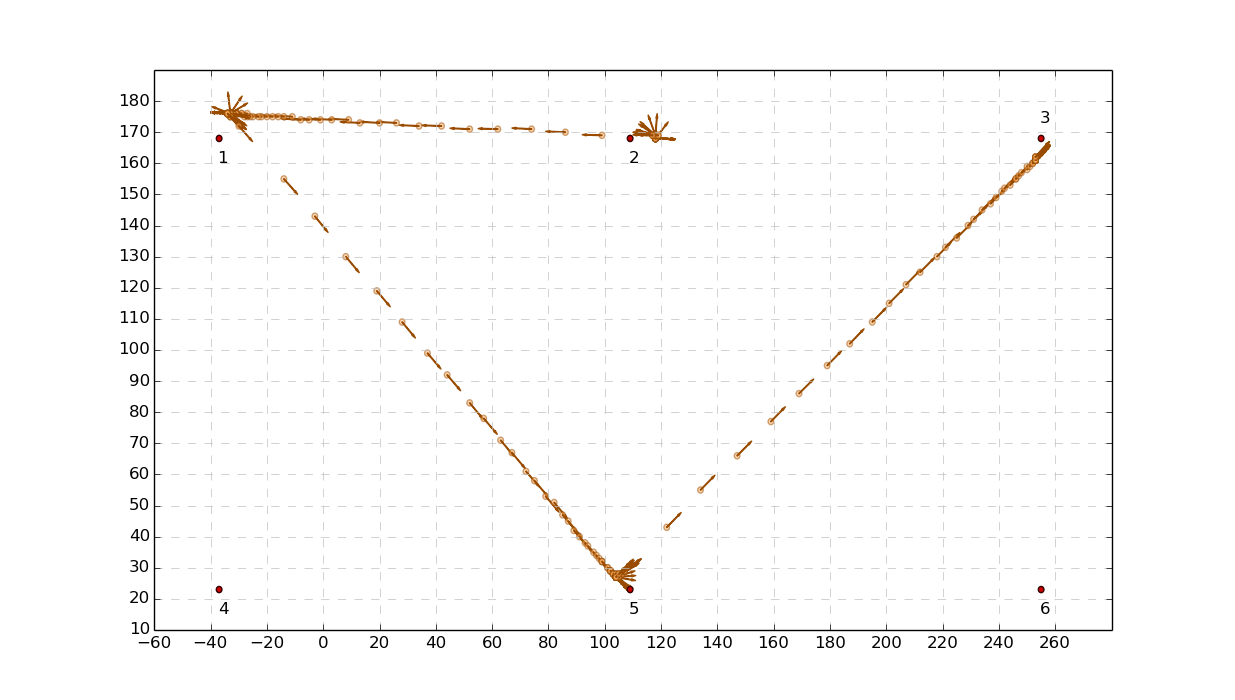
\includegraphics[scale=0.9]{./figures/task_22/figure_test.png}
      \caption{The robot's pose over time. Starting point is node 2.}
      \label{fig:22_map_plus_bearing}
    \end{figure}
\end{sidewaysfigure}

It wasn't before this experiment that we considered a
positive $K_{\omega}^T$, instead of a negative one, as the theoretical analysis
pointed to. The second component of the line-following controller showed
significantly worse performance when $K_{\omega}^T < 0$ than when $K_{\omega}^T > 0$.

When the robot was asked to go from node 2 to node 1, the angle between it and
node 1 was $1.68^{\circ} < \xi = 4^{\circ}$. Hence, the robot first executed
line-following, and not rotation. The augmented error in distance,
relative to the other two, is hence the fact that $K_{\omega}^T < 0$ during the
experimental phase.

Figure \ref{fig:22_map_7_xyt} illustrates the evolution of the position of the
robot over time.

\begin{figure}[H]\centering
  \scalebox{0.7}{% This file was created by matlab2tikz.
%
%The latest updates can be retrieved from
%  http://www.mathworks.com/matlabcentral/fileexchange/22022-matlab2tikz-matlab2tikz
%where you can also make suggestions and rate matlab2tikz.
%
\definecolor{mycolor1}{rgb}{0.00000,0.44700,0.74100}%
%
\begin{tikzpicture}

\begin{axis}[%
width=8in,
height=6.121in,
at={(1.342in,0.826in)},
scale only axis,
xmin=-0.85,
xmax=3,
tick align=outside,
xmajorgrids,
ymin=-0.2,
ymax=2,
ymajorgrids,
zmin=0,
zmax=180,
zmajorgrids,
view={-72.5}{40},
axis background/.style={fill=white},
axis x line*=bottom,
axis y line*=left,
axis z line*=left
]
\addplot3 [color=mycolor1,solid]
 table[row sep=crcr] {%
1.18	1.68	0\\
1.18	1.68	0.016667\\
1.18	1.68	0.033334\\
1.18	1.68	0.05\\
1.18	1.68	0.066667\\
1.18	1.68	0.083334\\
1.18	1.68	0.1\\
1.18	1.68	0.116667\\
1.18	1.68	0.133334\\
1.18	1.68	0.15\\
1.18	1.68	0.166667\\
1.18	1.68	0.183334\\
1.18	1.68	0.191667\\
1.18	1.68	0.208334\\
1.18	1.68	0.225\\
1.18	1.68	0.241667\\
1.18	1.68	0.258334\\
1.18	1.68	0.275\\
1.18	1.68	0.291667\\
1.18	1.68	0.308334\\
1.18	1.68	0.325\\
1.18	1.68	0.341667\\
1.18	1.68	0.358334\\
1.18	1.68	0.375\\
1.18	1.68	0.383334\\
1.18	1.68	0.4\\
1.18	1.68	0.416667\\
1.18	1.68	0.433334\\
1.18	1.68	0.45\\
1.18	1.68	0.466667\\
1.18	1.68	0.483334\\
1.18	1.68	0.5\\
1.18	1.68	0.516667\\
1.18	1.68	0.533334\\
1.18	1.68	0.55\\
1.18	1.68	0.566667\\
1.18	1.68	0.583334\\
1.18	1.68	0.591667\\
1.18	1.68	0.608334\\
1.18	1.68	0.625\\
1.18	1.68	0.641667\\
1.18	1.68	0.658334\\
1.18	1.68	0.675\\
1.18	1.68	0.691667\\
1.18	1.68	0.708334\\
1.18	1.68	0.725\\
1.18	1.68	0.741667\\
1.18	1.68	0.758334\\
1.18	1.68	0.775\\
1.18	1.68	0.783334\\
1.18	1.68	0.8\\
1.18	1.68	0.816667\\
1.18	1.68	0.833334\\
1.18	1.68	0.85\\
1.18	1.68	0.866667\\
1.18	1.68	0.883334\\
1.18	1.68	0.9\\
1.18	1.68	0.916667\\
1.18	1.68	0.933334\\
1.18	1.68	0.95\\
1.18	1.68	0.966667\\
1.18	1.68	0.983334\\
1.18	1.68	0.991667\\
1.18	1.68	1.008334\\
1.18	1.68	1.025\\
1.18	1.68	1.041667\\
1.18	1.68	1.058334\\
1.18	1.68	1.075\\
1.18	1.68	1.091667\\
1.18	1.68	1.108334\\
1.18	1.68	1.125\\
1.18	1.68	1.141667\\
1.18	1.68	1.158334\\
1.18	1.68	1.175\\
1.18	1.68	1.183334\\
1.18	1.68	1.2\\
1.18	1.68	1.216667\\
1.18	1.68	1.241667\\
1.18	1.68	1.25\\
1.18	1.68	1.266667\\
1.18	1.68	1.283334\\
1.18	1.68	1.3\\
1.18	1.68	1.316667\\
1.18	1.68	1.333334\\
1.18	1.68	1.35\\
1.18	1.68	1.366667\\
1.18	1.68	1.383334\\
1.18	1.68	1.391667\\
1.18	1.68	1.408334\\
1.18	1.68	1.425\\
1.18	1.68	1.441667\\
1.18	1.68	1.458334\\
1.18	1.68	1.475\\
1.18	1.68	1.491667\\
1.18	1.68	1.508334\\
1.18	1.68	1.525\\
1.18	1.68	1.541667\\
1.18	1.68	1.558334\\
1.18	1.68	1.575\\
1.18	1.68	1.583334\\
1.18	1.68	1.6\\
1.18	1.68	1.616667\\
1.18	1.68	1.633334\\
1.18	1.68	1.65\\
1.18	1.68	1.666667\\
1.18	1.68	1.683334\\
1.18	1.68	1.7\\
1.18	1.68	1.716667\\
1.18	1.68	1.733334\\
1.18	1.68	1.75\\
1.18	1.68	1.766667\\
1.18	1.68	1.783334\\
1.18	1.68	1.791667\\
1.18	1.68	1.808334\\
1.18	1.68	1.825\\
1.18	1.68	1.841667\\
1.18	1.68	1.858334\\
1.18	1.68	1.875\\
1.18	1.68	1.891667\\
1.18	1.68	1.908334\\
1.18	1.68	1.925\\
1.18	1.68	1.941667\\
1.18	1.68	1.958334\\
1.18	1.68	1.975\\
1.18	1.68	1.983334\\
1.18	1.68	2\\
1.18	1.68	2.016667\\
1.18	1.68	2.033334\\
1.18	1.68	2.05\\
1.18	1.68	2.066667\\
1.18	1.68	2.083334\\
1.18	1.68	2.1\\
1.18	1.68	2.116667\\
1.18	1.68	2.133334\\
1.18	1.68	2.15\\
1.18	1.68	2.166667\\
1.18	1.68	2.183334\\
1.18	1.68	2.191667\\
1.18	1.68	2.208334\\
1.18	1.68	2.225\\
1.18	1.68	2.241667\\
1.18	1.68	2.258334\\
1.18	1.68	2.275\\
1.18	1.68	2.291667\\
1.18	1.68	2.308334\\
1.18	1.68	2.325\\
1.18	1.68	2.341667\\
1.18	1.68	2.358334\\
1.18	1.68	2.375\\
1.18	1.68	2.383334\\
1.18	1.68	2.4\\
1.18	1.68	2.416667\\
1.18	1.68	2.433334\\
1.18	1.68	2.45\\
1.18	1.68	2.466667\\
1.18	1.68	2.483334\\
1.18	1.68	2.5\\
1.18	1.68	2.516667\\
1.18	1.68	2.533334\\
1.18	1.68	2.55\\
1.18	1.68	2.566667\\
1.18	1.68	2.583334\\
1.18	1.68	2.591667\\
1.18	1.68	2.608334\\
1.18	1.68	2.625\\
1.18	1.68	2.641667\\
1.18	1.68	2.658334\\
1.18	1.68	2.675\\
1.18	1.68	2.691667\\
1.18	1.68	2.708334\\
1.18	1.68	2.725\\
1.18	1.68	2.741667\\
1.18	1.68	2.758334\\
1.18	1.68	2.775\\
1.18	1.68	2.783334\\
1.18	1.68	2.8\\
1.18	1.68	2.816667\\
1.18	1.68	2.833334\\
1.18	1.68	2.85\\
1.18	1.68	2.866667\\
1.18	1.68	2.883334\\
1.18	1.68	2.9\\
1.18	1.68	2.916667\\
1.18	1.68	2.933334\\
1.18	1.68	2.95\\
1.18	1.68	2.966667\\
1.18	1.68	2.983334\\
1.18	1.68	2.991667\\
1.18	1.68	3.008334\\
1.18	1.68	3.025\\
1.18	1.68	3.041667\\
1.18	1.68	3.058334\\
1.18	1.68	3.075\\
1.18	1.68	3.091667\\
1.18	1.68	3.108334\\
1.18	1.68	3.125\\
1.18	1.68	3.141667\\
1.18	1.68	3.158334\\
1.18	1.68	3.175\\
1.18	1.68	3.183334\\
1.18	1.68	3.2\\
1.18	1.68	3.216667\\
1.18	1.68	3.233334\\
1.18	1.68	3.25\\
1.18	1.68	3.266667\\
1.18	1.68	3.283334\\
1.18	1.68	3.3\\
1.18	1.68	3.316667\\
1.18	1.68	3.333334\\
1.18	1.68	3.35\\
1.18	1.68	3.366667\\
1.18	1.68	3.375\\
1.18	1.68	3.391667\\
1.18	1.68	3.408334\\
1.18	1.68	3.425\\
1.18	1.68	3.441667\\
1.18	1.68	3.458334\\
1.18	1.68	3.475\\
1.18	1.68	3.491667\\
1.18	1.68	3.508334\\
1.18	1.68	3.525\\
1.18	1.68	3.541667\\
1.18	1.68	3.558334\\
1.18	1.68	3.575\\
1.18	1.68	3.583334\\
1.18	1.68	3.6\\
1.18	1.68	3.616667\\
1.18	1.68	3.633334\\
1.18	1.68	3.65\\
1.18	1.68	3.666667\\
1.18	1.68	3.683334\\
1.18	1.68	3.7\\
1.18	1.68	3.716667\\
1.18	1.68	3.733334\\
1.18	1.68	3.75\\
1.18	1.68	3.766667\\
1.18	1.68	3.783334\\
1.18	1.68	3.791667\\
1.18	1.68	3.808334\\
1.18	1.68	3.825\\
1.18	1.68	3.841667\\
1.18	1.68	3.858334\\
1.18	1.68	3.875\\
1.18	1.68	3.891667\\
1.18	1.68	3.908334\\
1.18	1.68	3.925\\
1.18	1.68	3.941667\\
1.18	1.68	3.958334\\
1.18	1.68	3.975\\
1.18	1.68	3.983334\\
1.18	1.68	4\\
1.18	1.68	4.016667\\
1.18	1.68	4.033334\\
1.18	1.68	4.05\\
1.18	1.68	4.066667\\
1.18	1.68	4.083334\\
1.18	1.68	4.1\\
1.18	1.68	4.116667\\
1.18	1.68	4.133334\\
1.18	1.68	4.15\\
1.18	1.68	4.166667\\
1.18	1.68	4.183334\\
1.18	1.68	4.191667\\
1.18	1.68	4.208334\\
1.18	1.68	4.225\\
1.18	1.68	4.241667\\
1.18	1.68	4.258334\\
1.18	1.68	4.275\\
1.18	1.68	4.291667\\
1.18	1.68	4.308334\\
1.18	1.68	4.325\\
1.18	1.68	4.341667\\
1.18	1.68	4.358334\\
1.18	1.68	4.375\\
1.18	1.68	4.383334\\
1.18	1.68	4.4\\
1.18	1.68	4.416667\\
1.18	1.68	4.433334\\
1.18	1.68	4.45\\
1.18	1.68	4.466667\\
1.18	1.68	4.483334\\
1.18	1.68	4.5\\
1.18	1.68	4.516667\\
1.18	1.68	4.533334\\
1.18	1.68	4.55\\
1.18	1.68	4.566667\\
1.18	1.68	4.583334\\
1.18	1.68	4.591667\\
1.18	1.68	4.608334\\
1.18	1.68	4.625\\
1.18	1.68	4.641667\\
1.18	1.68	4.658334\\
1.18	1.68	4.675\\
1.18	1.68	4.691667\\
1.18	1.68	4.708334\\
1.18	1.68	4.725\\
1.18	1.68	4.741667\\
1.18	1.68	4.758334\\
1.18	1.68	4.775\\
1.18	1.68	4.783334\\
1.18	1.68	4.8\\
1.18	1.68	4.816667\\
1.18	1.68	4.833334\\
1.18	1.68	4.85\\
1.18	1.68	4.866667\\
1.18	1.68	4.883334\\
1.18	1.68	4.9\\
1.18	1.68	4.916667\\
1.18	1.68	4.933334\\
1.18	1.68	4.95\\
1.18	1.68	4.966667\\
1.18	1.68	4.983334\\
1.18	1.68	4.991667\\
1.18	1.68	5.008334\\
1.18	1.68	5.025\\
1.18	1.68	5.041667\\
1.18	1.68	5.058334\\
1.18	1.68	5.075\\
1.18	1.68	5.091667\\
1.18	1.68	5.108334\\
1.18	1.68	5.125\\
1.18	1.68	5.141667\\
1.18	1.68	5.158334\\
1.18	1.68	5.175\\
1.18	1.68	5.183334\\
1.18	1.68	5.2\\
1.18	1.68	5.216667\\
1.18	1.68	5.233334\\
1.18	1.68	5.25\\
1.18	1.68	5.266667\\
1.18	1.68	5.283334\\
1.18	1.68	5.3\\
1.18	1.68	5.316667\\
1.18	1.68	5.333334\\
1.18	1.68	5.35\\
1.18	1.68	5.366667\\
1.18	1.68	5.383334\\
1.18	1.68	5.391667\\
1.18	1.68	5.408334\\
1.18	1.68	5.425\\
1.18	1.68	5.441667\\
1.18	1.68	5.458334\\
1.18	1.68	5.475\\
1.18	1.68	5.491667\\
1.18	1.68	5.508334\\
1.18	1.68	5.525\\
1.18	1.68	5.541667\\
1.18	1.68	5.558334\\
1.18	1.68	5.575\\
1.18	1.68	5.583334\\
1.18	1.68	5.6\\
1.18	1.68	5.616667\\
1.18	1.68	5.633334\\
1.18	1.68	5.65\\
1.18	1.68	5.666667\\
1.18	1.68	5.683334\\
1.18	1.68	5.7\\
1.18	1.68	5.716667\\
1.18	1.68	5.733334\\
1.18	1.68	5.75\\
1.18	1.68	5.766667\\
1.18	1.68	5.783334\\
1.18	1.68	5.791667\\
1.18	1.68	5.808334\\
1.18	1.68	5.825\\
1.18	1.68	5.841667\\
1.18	1.68	5.858334\\
1.18	1.68	5.875\\
1.18	1.68	5.891667\\
1.18	1.68	5.908334\\
1.18	1.68	5.925\\
1.18	1.68	5.941667\\
1.18	1.68	5.958334\\
1.18	1.68	5.975\\
1.18	1.68	5.983334\\
1.18	1.68	6\\
1.18	1.68	6.016667\\
1.18	1.68	6.033334\\
1.18	1.68	6.05\\
1.18	1.68	6.066667\\
1.18	1.68	6.083334\\
1.18	1.68	6.1\\
1.18	1.68	6.116667\\
1.18	1.68	6.133334\\
1.18	1.68	6.15\\
1.18	1.68	6.166667\\
1.18	1.68	6.183334\\
1.18	1.68	6.191667\\
1.18	1.68	6.208334\\
1.18	1.68	6.225\\
1.18	1.68	6.241667\\
1.18	1.68	6.258334\\
1.18	1.68	6.275\\
1.18	1.68	6.291667\\
1.18	1.68	6.308334\\
1.18	1.68	6.325\\
1.18	1.68	6.341667\\
1.18	1.68	6.358334\\
1.18	1.68	6.375\\
1.18	1.68	6.383334\\
1.18	1.68	6.4\\
1.18	1.68	6.416667\\
1.18	1.68	6.433334\\
1.18	1.68	6.45\\
1.18	1.68	6.466667\\
1.18	1.68	6.483334\\
1.18	1.68	6.5\\
1.18	1.68	6.516667\\
1.18	1.68	6.533334\\
1.18	1.68	6.55\\
1.18	1.68	6.566667\\
1.18	1.68	6.583334\\
1.18	1.68	6.591667\\
1.18	1.68	6.608334\\
1.18	1.68	6.625\\
1.18	1.68	6.641667\\
1.18	1.68	6.658334\\
1.18	1.68	6.675\\
1.18	1.68	6.691667\\
1.18	1.68	6.708334\\
1.18	1.68	6.725\\
1.18	1.68	6.741667\\
1.18	1.68	6.758334\\
1.18	1.68	6.775\\
1.18	1.68	6.783334\\
1.18	1.68	6.8\\
1.18	1.68	6.816667\\
1.18	1.68	6.833334\\
1.18	1.68	6.85\\
1.18	1.68	6.866667\\
1.18	1.68	6.883334\\
1.18	1.68	6.9\\
1.18	1.68	6.916667\\
1.18	1.68	6.933334\\
1.18	1.68	6.95\\
1.18	1.68	6.966667\\
1.18	1.68	6.983334\\
1.18	1.68	6.991667\\
1.18	1.68	7.008334\\
1.18	1.68	7.025\\
1.18	1.68	7.041667\\
1.18	1.68	7.058334\\
1.18	1.68	7.075\\
1.18	1.68	7.091667\\
1.18	1.68	7.108334\\
1.18	1.68	7.125\\
1.18	1.68	7.141667\\
1.18	1.68	7.158334\\
1.18	1.68	7.175\\
1.18	1.68	7.183334\\
1.18	1.68	7.2\\
1.18	1.68	7.216667\\
1.18	1.68	7.233334\\
1.18	1.68	7.25\\
1.18	1.68	7.266667\\
1.18	1.68	7.283334\\
1.18	1.68	7.3\\
1.18	1.68	7.316667\\
1.18	1.68	7.333334\\
1.18	1.68	7.35\\
1.18	1.68	7.366667\\
1.18	1.68	7.383334\\
1.18	1.68	7.391667\\
1.18	1.68	7.408334\\
1.18	1.68	7.425\\
1.18	1.68	7.441667\\
1.18	1.68	7.458334\\
1.18	1.68	7.475\\
1.18	1.68	7.491667\\
1.18	1.68	7.508334\\
1.18	1.68	7.525\\
1.18	1.68	7.541667\\
1.18	1.68	7.558334\\
1.18	1.68	7.575\\
1.18	1.68	7.583334\\
1.18	1.68	7.6\\
1.18	1.68	7.616667\\
1.18	1.68	7.633334\\
1.18	1.68	7.65\\
1.18	1.68	7.666667\\
1.18	1.68	7.683334\\
1.18	1.68	7.7\\
1.18	1.68	7.716667\\
1.18	1.68	7.733334\\
1.18	1.68	7.75\\
1.18	1.68	7.766667\\
1.18	1.68	7.783334\\
1.18	1.68	7.791667\\
1.18	1.68	7.808334\\
1.18	1.68	7.825\\
1.18	1.68	7.841667\\
1.18	1.68	7.858334\\
1.18	1.68	7.875\\
1.18	1.68	7.891667\\
1.18	1.68	7.908334\\
1.18	1.68	7.925\\
1.18	1.68	7.941667\\
1.18	1.68	7.958334\\
1.18	1.68	7.975\\
1.18	1.68	7.991667\\
1.18	1.68	8\\
1.18	1.68	8.016667\\
1.18	1.68	8.033334\\
1.18	1.68	8.05\\
1.18	1.68	8.066667\\
1.18	1.68	8.083334\\
1.18	1.68	8.1\\
1.18	1.68	8.116667\\
1.18	1.68	8.133334\\
1.18	1.68	8.15\\
1.18	1.68	8.166667\\
1.18	1.68	8.183334\\
1.18	1.68	8.191667\\
1.18	1.68	8.208334\\
1.18	1.68	8.225\\
1.18	1.68	8.241667\\
1.18	1.68	8.258334\\
1.18	1.68	8.275\\
1.18	1.68	8.291667\\
1.18	1.68	8.308334\\
1.18	1.68	8.325\\
1.18	1.68	8.341667\\
1.18	1.68	8.358334\\
1.18	1.68	8.375\\
1.18	1.68	8.383334\\
1.18	1.68	8.4\\
1.18	1.68	8.416667\\
1.18	1.68	8.433334\\
1.18	1.68	8.45\\
1.18	1.68	8.466667\\
1.18	1.68	8.483334\\
1.18	1.68	8.5\\
1.18	1.68	8.516667\\
1.18	1.68	8.533334\\
1.18	1.68	8.55\\
1.18	1.68	8.566667\\
1.18	1.68	8.583334\\
1.18	1.68	8.591667\\
1.18	1.68	8.608334\\
1.18	1.68	8.625\\
1.18	1.68	8.641667\\
1.18	1.68	8.658334\\
1.18	1.68	8.675\\
1.18	1.68	8.691667\\
1.18	1.68	8.708334\\
1.18	1.68	8.725\\
1.18	1.68	8.741667\\
1.18	1.68	8.758334\\
1.18	1.68	8.775\\
1.18	1.68	8.783334\\
1.18	1.68	8.8\\
1.18	1.68	8.816667\\
1.18	1.68	8.833334\\
1.18	1.68	8.85\\
1.18	1.68	8.866667\\
1.18	1.68	8.883334\\
1.18	1.68	8.9\\
1.18	1.68	8.916667\\
1.18	1.68	8.933334\\
1.18	1.68	8.95\\
1.18	1.68	8.966667\\
1.18	1.68	8.983334\\
1.18	1.68	8.991667\\
1.18	1.68	9.008334\\
1.18	1.68	9.025\\
1.18	1.68	9.041667\\
1.18	1.68	9.058334\\
1.18	1.68	9.075\\
1.18	1.68	9.091667\\
1.18	1.68	9.108334\\
1.18	1.68	9.125\\
1.18	1.68	9.141667\\
1.18	1.68	9.158334\\
1.18	1.68	9.175\\
1.18	1.68	9.183334\\
1.18	1.68	9.2\\
1.18	1.68	9.216667\\
1.18	1.68	9.233334\\
1.18	1.68	9.25\\
1.18	1.68	9.266667\\
1.18	1.68	9.283334\\
1.18	1.68	9.3\\
1.18	1.68	9.316667\\
1.18	1.68	9.333334\\
1.18	1.68	9.35\\
1.18	1.68	9.366667\\
1.18	1.68	9.383334\\
1.18	1.68	9.391667\\
1.18	1.68	9.408334\\
1.18	1.68	9.425\\
1.18	1.68	9.441667\\
1.18	1.68	9.458334\\
1.18	1.68	9.475\\
1.18	1.68	9.491667\\
1.18	1.68	9.508334\\
1.18	1.68	9.525\\
1.18	1.68	9.541667\\
1.18	1.68	9.558334\\
1.18	1.68	9.575\\
1.18	1.68	9.583334\\
1.18	1.68	9.6\\
1.18	1.68	9.616667\\
1.18	1.68	9.633334\\
1.18	1.68	9.65\\
1.18	1.68	9.666667\\
1.18	1.68	9.683334\\
1.18	1.68	9.7\\
1.18	1.68	9.716667\\
1.18	1.68	9.733334\\
1.18	1.68	9.75\\
1.18	1.68	9.766667\\
1.18	1.68	9.783334\\
1.18	1.68	9.791667\\
1.18	1.68	9.808334\\
1.18	1.68	9.825\\
1.18	1.68	9.841667\\
1.18	1.68	9.858334\\
1.18	1.68	9.875\\
1.18	1.68	9.891667\\
1.18	1.68	9.908334\\
1.18	1.68	9.925\\
1.18	1.68	9.941667\\
1.18	1.68	9.958334\\
1.18	1.68	9.975\\
1.18	1.68	9.983334\\
1.18	1.68	10\\
1.18	1.68	10.016667\\
1.18	1.68	10.033334\\
1.18	1.68	10.05\\
1.18	1.68	10.066667\\
1.18	1.68	10.083334\\
1.18	1.68	10.1\\
1.18	1.68	10.116667\\
1.18	1.68	10.133334\\
1.18	1.68	10.15\\
1.18	1.68	10.166667\\
1.18	1.68	10.183334\\
1.18	1.68	10.191667\\
1.18	1.68	10.208334\\
1.18	1.68	10.225\\
1.18	1.68	10.241667\\
1.18	1.68	10.258334\\
1.18	1.68	10.275\\
1.18	1.68	10.291667\\
1.18	1.68	10.308334\\
1.18	1.68	10.325\\
1.18	1.68	10.341667\\
1.18	1.68	10.358334\\
1.18	1.68	10.375\\
1.18	1.68	10.391667\\
1.18	1.68	10.4\\
1.18	1.68	10.416667\\
1.18	1.68	10.433334\\
1.18	1.68	10.45\\
1.18	1.68	10.466667\\
1.18	1.68	10.483334\\
1.18	1.68	10.5\\
1.18	1.68	10.516667\\
1.18	1.68	10.533334\\
1.18	1.68	10.55\\
1.18	1.68	10.566667\\
1.18	1.68	10.583334\\
1.18	1.68	10.591667\\
1.18	1.68	10.608334\\
1.18	1.68	10.625\\
1.18	1.68	10.641667\\
1.18	1.68	10.658334\\
1.18	1.68	10.675\\
1.18	1.68	10.691667\\
1.18	1.68	10.708334\\
1.18	1.68	10.725\\
1.18	1.68	10.741667\\
1.18	1.68	10.758334\\
1.18	1.68	10.775\\
1.18	1.68	10.791667\\
1.18	1.68	10.8\\
1.18	1.68	10.816667\\
1.18	1.68	10.833334\\
1.18	1.68	10.85\\
1.18	1.68	10.866667\\
1.18	1.68	10.883334\\
1.18	1.68	10.9\\
1.18	1.68	10.916667\\
1.18	1.68	10.933334\\
1.18	1.68	10.95\\
1.18	1.68	10.966667\\
1.18	1.68	10.983334\\
1.18	1.68	10.991667\\
1.18	1.68	11.008334\\
1.18	1.68	11.025\\
1.18	1.68	11.041667\\
1.18	1.68	11.058334\\
1.18	1.68	11.075\\
1.18	1.68	11.091667\\
1.18	1.68	11.108334\\
1.18	1.68	11.125\\
1.18	1.68	11.141667\\
1.18	1.68	11.158334\\
1.18	1.68	11.175\\
1.18	1.68	11.183334\\
1.18	1.68	11.2\\
1.18	1.68	11.216667\\
1.18	1.68	11.241667\\
1.18	1.68	11.25\\
1.18	1.68	11.266667\\
1.18	1.68	11.283334\\
1.18	1.68	11.3\\
1.18	1.68	11.316667\\
1.18	1.68	11.333334\\
1.18	1.68	11.35\\
1.18	1.68	11.366667\\
1.18	1.68	11.383334\\
1.18	1.68	11.391667\\
1.18	1.68	11.408334\\
1.18	1.68	11.425\\
1.18	1.68	11.441667\\
1.18	1.68	11.458334\\
1.18	1.68	11.475\\
1.18	1.68	11.491667\\
1.18	1.68	11.508334\\
1.18	1.68	11.525\\
1.18	1.68	11.541667\\
1.18	1.68	11.558334\\
1.18	1.68	11.575\\
1.18	1.68	11.591667\\
1.18	1.68	11.6\\
1.18	1.68	11.625\\
1.18	1.68	11.633334\\
1.18	1.68	11.65\\
1.18	1.68	11.666667\\
1.18	1.68	11.683334\\
1.18	1.68	11.7\\
1.18	1.68	11.716667\\
1.18	1.68	11.733334\\
1.18	1.68	11.75\\
1.18	1.68	11.766667\\
1.18	1.68	11.783334\\
1.18	1.68	11.791667\\
1.18	1.68	11.808334\\
1.18	1.68	11.825\\
1.18	1.68	11.841667\\
1.18	1.68	11.858334\\
1.18	1.68	11.875\\
1.18	1.68	11.891667\\
1.18	1.68	11.908334\\
1.18	1.68	11.925\\
1.18	1.68	11.941667\\
1.18	1.68	11.958334\\
1.18	1.68	11.975\\
1.18	1.68	11.983334\\
1.18	1.68	12\\
1.18	1.68	12.016667\\
1.18	1.68	12.033334\\
1.18	1.68	12.05\\
1.18	1.68	12.066667\\
1.18	1.68	12.083334\\
1.18	1.68	12.1\\
1.18	1.68	12.116667\\
1.18	1.68	12.133334\\
1.18	1.68	12.15\\
1.18	1.68	12.166667\\
1.18	1.68	12.183334\\
1.18	1.68	12.191667\\
1.18	1.68	12.208334\\
1.18	1.68	12.225\\
1.18	1.68	12.241667\\
1.18	1.68	12.258334\\
1.18	1.68	12.275\\
1.18	1.68	12.291667\\
1.18	1.68	12.308334\\
1.18	1.68	12.325\\
1.18	1.68	12.341667\\
1.18	1.68	12.358334\\
1.18	1.68	12.375\\
1.18	1.68	12.391667\\
1.18	1.68	12.4\\
1.18	1.68	12.416667\\
1.18	1.68	12.433334\\
1.18	1.68	12.45\\
1.18	1.68	12.466667\\
1.18	1.68	12.483334\\
1.18	1.68	12.5\\
1.18	1.68	12.516667\\
1.18	1.68	12.533334\\
1.18	1.68	12.55\\
1.18	1.68	12.566667\\
1.18	1.68	12.583334\\
1.18	1.68	12.6\\
1.18	1.68	12.608334\\
1.18	1.68	12.625\\
1.18	1.68	12.641667\\
1.18	1.68	12.658334\\
1.18	1.68	12.675\\
1.18	1.68	12.691667\\
1.18	1.68	12.708334\\
1.18	1.68	12.725\\
1.18	1.68	12.741667\\
1.18	1.68	12.758334\\
1.18	1.68	12.775\\
1.18	1.68	12.791667\\
1.18	1.68	12.8\\
1.18	1.68	12.816667\\
1.18	1.68	12.833334\\
1.18	1.68	12.85\\
1.18	1.68	12.866667\\
1.18	1.68	12.883334\\
1.18	1.68	12.9\\
1.18	1.68	12.916667\\
1.18	1.68	12.933334\\
1.18	1.68	12.95\\
1.18	1.68	12.966667\\
1.18	1.68	12.983334\\
1.18	1.68	12.991667\\
1.18	1.68	13.008334\\
1.18	1.68	13.025\\
1.18	1.68	13.041667\\
1.18	1.68	13.058334\\
1.18	1.68	13.075\\
1.18	1.68	13.091667\\
1.18	1.68	13.108334\\
1.18	1.68	13.125\\
1.18	1.68	13.141667\\
1.18	1.68	13.158334\\
1.18	1.68	13.175\\
1.18	1.68	13.191667\\
1.18	1.68	13.2\\
1.18	1.68	13.216667\\
1.18	1.69	13.241667\\
1.18	1.69	13.25\\
1.18	1.69	13.266667\\
1.18	1.69	13.283334\\
1.18	1.69	13.3\\
1.18	1.69	13.316667\\
1.18	1.69	13.333334\\
1.18	1.69	13.35\\
1.18	1.69	13.366667\\
1.18	1.69	13.375\\
1.18	1.69	13.391667\\
1.18	1.69	13.408334\\
1.18	1.69	13.425\\
1.18	1.69	13.441667\\
1.18	1.69	13.458334\\
1.18	1.69	13.475\\
1.18	1.69	13.491667\\
1.18	1.69	13.508334\\
1.18	1.69	13.525\\
1.18	1.68	13.541667\\
1.18	1.69	13.558334\\
1.18	1.69	13.575\\
1.18	1.69	13.591667\\
1.18	1.69	13.6\\
1.18	1.69	13.616667\\
1.18	1.69	13.633334\\
1.18	1.69	13.65\\
1.18	1.69	13.666667\\
1.18	1.69	13.683334\\
1.18	1.69	13.7\\
1.18	1.69	13.716667\\
1.18	1.69	13.733334\\
1.18	1.69	13.75\\
1.18	1.69	13.766667\\
1.18	1.69	13.783334\\
1.18	1.69	13.791667\\
1.18	1.69	13.808334\\
1.18	1.69	13.825\\
1.18	1.69	13.841667\\
1.18	1.69	13.858334\\
1.18	1.69	13.875\\
1.18	1.69	13.891667\\
1.18	1.69	13.908334\\
1.18	1.69	13.925\\
1.18	1.69	13.941667\\
1.18	1.69	13.958334\\
1.18	1.69	13.975\\
1.18	1.69	13.983334\\
1.18	1.69	14\\
1.18	1.69	14.016667\\
1.18	1.69	14.033334\\
1.18	1.69	14.05\\
1.18	1.69	14.066667\\
1.18	1.69	14.083334\\
1.18	1.69	14.1\\
1.18	1.69	14.116667\\
1.18	1.69	14.133334\\
1.18	1.69	14.15\\
1.18	1.69	14.166667\\
1.18	1.69	14.183334\\
1.18	1.69	14.191667\\
1.18	1.69	14.208334\\
1.18	1.69	14.225\\
1.18	1.69	14.241667\\
1.18	1.69	14.258334\\
1.18	1.69	14.275\\
1.18	1.69	14.291667\\
1.18	1.69	14.308334\\
1.18	1.69	14.325\\
1.18	1.69	14.341667\\
1.18	1.69	14.358334\\
1.18	1.69	14.375\\
1.18	1.69	14.391667\\
1.18	1.69	14.4\\
1.18	1.69	14.416667\\
1.18	1.69	14.433334\\
1.18	1.69	14.45\\
1.18	1.69	14.466667\\
1.18	1.69	14.483334\\
1.18	1.69	14.5\\
1.18	1.69	14.516667\\
1.18	1.69	14.533334\\
1.18	1.69	14.55\\
1.18	1.69	14.566667\\
1.18	1.69	14.583334\\
1.18	1.69	14.591667\\
1.18	1.69	14.608334\\
1.18	1.69	14.625\\
1.18	1.69	14.641667\\
1.18	1.69	14.658334\\
1.18	1.69	14.675\\
1.18	1.69	14.691667\\
1.18	1.69	14.708334\\
1.18	1.69	14.725\\
1.18	1.69	14.741667\\
1.18	1.69	14.758334\\
1.18	1.69	14.775\\
1.18	1.69	14.783334\\
1.18	1.69	14.808334\\
1.18	1.69	14.816667\\
1.18	1.69	14.833334\\
1.18	1.69	14.85\\
1.18	1.69	14.866667\\
1.18	1.69	14.883334\\
1.18	1.69	14.9\\
1.18	1.69	14.916667\\
1.18	1.69	14.933334\\
1.18	1.69	14.95\\
1.18	1.69	14.966667\\
1.18	1.69	14.983334\\
1.18	1.69	14.991667\\
1.18	1.69	15.008334\\
1.18	1.69	15.025\\
1.18	1.69	15.041667\\
1.18	1.69	15.058334\\
1.18	1.69	15.075\\
1.18	1.69	15.091667\\
1.18	1.69	15.108334\\
1.18	1.69	15.125\\
1.18	1.69	15.141667\\
1.18	1.69	15.158334\\
1.18	1.69	15.175\\
1.18	1.69	15.183334\\
1.18	1.69	15.208334\\
1.18	1.69	15.216667\\
1.18	1.69	15.241667\\
1.18	1.69	15.25\\
1.18	1.69	15.266667\\
1.18	1.69	15.283334\\
1.18	1.69	15.3\\
1.18	1.69	15.316667\\
1.18	1.69	15.333334\\
1.18	1.69	15.35\\
1.18	1.69	15.366667\\
1.18	1.69	15.383334\\
1.18	1.69	15.391667\\
1.18	1.69	15.408334\\
1.18	1.69	15.425\\
1.18	1.69	15.441667\\
1.18	1.69	15.458334\\
1.18	1.69	15.475\\
1.18	1.69	15.491667\\
1.18	1.69	15.508334\\
1.18	1.69	15.525\\
1.18	1.69	15.541667\\
1.18	1.69	15.558334\\
1.18	1.69	15.575\\
1.18	1.69	15.591667\\
1.18	1.69	15.6\\
1.18	1.69	15.616667\\
1.18	1.69	15.633334\\
1.18	1.69	15.65\\
1.18	1.69	15.666667\\
1.18	1.69	15.683334\\
1.18	1.69	15.7\\
1.18	1.69	15.716667\\
1.18	1.69	15.733334\\
1.18	1.69	15.75\\
1.18	1.69	15.766667\\
1.18	1.69	15.783334\\
1.18	1.69	15.791667\\
1.18	1.69	15.808334\\
1.18	1.69	15.825\\
1.18	1.69	15.841667\\
1.18	1.69	15.858334\\
1.18	1.69	15.875\\
1.18	1.69	15.891667\\
1.18	1.69	15.908334\\
1.18	1.69	15.925\\
1.18	1.69	15.941667\\
1.18	1.69	15.958334\\
1.18	1.69	15.975\\
1.18	1.69	15.991667\\
1.18	1.69	16\\
1.18	1.69	16.016667\\
1.18	1.69	16.033334\\
1.18	1.69	16.05\\
1.18	1.69	16.066667\\
1.18	1.69	16.083334\\
1.18	1.69	16.1\\
1.18	1.69	16.116667\\
1.18	1.69	16.133334\\
1.18	1.69	16.15\\
1.18	1.69	16.166667\\
1.18	1.69	16.183334\\
1.18	1.69	16.191667\\
1.18	1.69	16.208334\\
1.18	1.69	16.225\\
1.18	1.69	16.241667\\
1.18	1.69	16.258334\\
1.18	1.69	16.275\\
1.18	1.69	16.291667\\
1.18	1.69	16.308334\\
1.18	1.69	16.325\\
1.18	1.69	16.341667\\
1.18	1.69	16.358334\\
1.18	1.69	16.375\\
1.18	1.69	16.391667\\
1.18	1.69	16.4\\
1.18	1.69	16.416667\\
1.18	1.69	16.433334\\
1.18	1.69	16.45\\
1.18	1.69	16.466667\\
1.17	1.69	16.483334\\
1.17	1.69	16.5\\
1.17	1.69	16.516667\\
1.18	1.69	16.533334\\
1.17	1.69	16.55\\
1.17	1.69	16.566667\\
1.17	1.69	16.583334\\
1.17	1.69	16.591667\\
1.17	1.69	16.608334\\
1.17	1.69	16.625\\
1.17	1.69	16.641667\\
1.17	1.69	16.658334\\
1.17	1.69	16.675\\
1.17	1.69	16.691667\\
1.17	1.69	16.708334\\
1.17	1.69	16.725\\
1.17	1.69	16.741667\\
1.17	1.69	16.758334\\
1.17	1.69	16.775\\
1.17	1.69	16.791667\\
1.17	1.69	16.808334\\
1.17	1.69	16.816667\\
1.17	1.69	16.833334\\
1.17	1.69	16.85\\
1.17	1.69	16.866667\\
1.17	1.69	16.883334\\
1.17	1.69	16.9\\
1.17	1.69	16.916667\\
1.17	1.69	16.933334\\
1.17	1.69	16.95\\
1.17	1.69	16.966667\\
1.17	1.69	16.983334\\
1.17	1.69	16.991667\\
1.17	1.69	17.008334\\
1.17	1.69	17.025\\
1.17	1.69	17.041667\\
1.17	1.69	17.058334\\
1.17	1.69	17.075\\
1.17	1.69	17.091667\\
1.17	1.69	17.108334\\
1.17	1.69	17.125\\
1.17	1.69	17.141667\\
1.17	1.69	17.158334\\
1.17	1.69	17.175\\
1.17	1.69	17.191667\\
1.17	1.69	17.208334\\
1.17	1.69	17.216667\\
1.17	1.69	17.241667\\
1.17	1.69	17.25\\
1.17	1.69	17.266667\\
1.17	1.69	17.283334\\
1.17	1.69	17.3\\
1.17	1.69	17.316667\\
1.18	1.69	17.333334\\
1.18	1.69	17.35\\
1.18	1.69	17.366667\\
1.18	1.69	17.383334\\
1.18	1.69	17.391667\\
1.18	1.69	17.408334\\
1.18	1.69	17.425\\
1.18	1.69	17.441667\\
1.18	1.69	17.458334\\
1.18	1.69	17.475\\
1.18	1.69	17.491667\\
1.18	1.69	17.508334\\
1.18	1.69	17.525\\
1.18	1.69	17.541667\\
1.18	1.69	17.558334\\
1.18	1.69	17.575\\
1.18	1.69	17.591667\\
1.18	1.69	17.608334\\
1.18	1.69	17.616667\\
1.18	1.69	17.633334\\
1.18	1.69	17.65\\
1.18	1.69	17.666667\\
1.18	1.69	17.683334\\
1.18	1.69	17.7\\
1.18	1.69	17.716667\\
1.18	1.69	17.733334\\
1.18	1.69	17.75\\
1.18	1.69	17.766667\\
1.18	1.69	17.783334\\
1.18	1.69	17.791667\\
1.18	1.69	17.808334\\
1.18	1.69	17.825\\
1.18	1.69	17.841667\\
1.18	1.69	17.858334\\
1.18	1.69	17.875\\
1.18	1.69	17.891667\\
1.18	1.69	17.908334\\
1.18	1.69	17.925\\
1.18	1.69	17.941667\\
1.18	1.69	17.958334\\
1.18	1.69	17.975\\
1.18	1.69	17.991667\\
1.18	1.69	18.008334\\
1.18	1.69	18.016667\\
1.18	1.69	18.033334\\
1.18	1.69	18.05\\
1.18	1.69	18.066667\\
1.18	1.69	18.083334\\
1.18	1.69	18.1\\
1.18	1.69	18.116667\\
1.18	1.69	18.133334\\
1.18	1.69	18.15\\
1.18	1.69	18.166667\\
1.18	1.69	18.183334\\
1.18	1.69	18.191667\\
1.18	1.69	18.208334\\
1.18	1.69	18.225\\
1.18	1.69	18.241667\\
1.18	1.69	18.258334\\
1.18	1.69	18.275\\
1.18	1.69	18.291667\\
1.18	1.69	18.308334\\
1.18	1.69	18.325\\
1.18	1.69	18.341667\\
1.18	1.69	18.358334\\
1.18	1.69	18.375\\
1.18	1.69	18.391667\\
1.18	1.69	18.408334\\
1.18	1.69	18.416667\\
1.18	1.69	18.433334\\
1.18	1.69	18.45\\
1.18	1.69	18.466667\\
1.18	1.69	18.483334\\
1.18	1.69	18.5\\
1.18	1.69	18.516667\\
1.18	1.69	18.533334\\
1.18	1.69	18.55\\
1.18	1.69	18.566667\\
1.18	1.69	18.583334\\
1.18	1.69	18.591667\\
1.18	1.69	18.608334\\
1.18	1.69	18.625\\
1.18	1.69	18.641667\\
1.18	1.69	18.658334\\
1.18	1.69	18.675\\
1.18	1.69	18.691667\\
1.18	1.69	18.708334\\
1.18	1.69	18.725\\
1.18	1.69	18.741667\\
1.18	1.69	18.758334\\
1.18	1.69	18.775\\
1.18	1.69	18.791667\\
1.18	1.69	18.808334\\
1.18	1.69	18.816667\\
1.18	1.69	18.833334\\
1.18	1.69	18.85\\
1.18	1.69	18.866667\\
1.18	1.69	18.883334\\
1.18	1.69	18.9\\
1.18	1.69	18.916667\\
1.18	1.69	18.933334\\
1.18	1.69	18.95\\
1.18	1.69	18.966667\\
1.18	1.69	18.983334\\
1.18	1.69	18.991667\\
1.18	1.69	19.008334\\
1.18	1.69	19.025\\
1.18	1.69	19.041667\\
1.18	1.69	19.058334\\
1.18	1.69	19.075\\
1.18	1.69	19.091667\\
1.18	1.69	19.108334\\
1.18	1.69	19.125\\
1.18	1.69	19.141667\\
1.18	1.69	19.158334\\
1.18	1.69	19.175\\
1.18	1.69	19.191667\\
1.18	1.69	19.2\\
1.18	1.69	19.216667\\
1.18	1.69	19.233334\\
1.18	1.69	19.25\\
1.18	1.69	19.266667\\
1.18	1.69	19.283334\\
1.18	1.69	19.3\\
1.18	1.69	19.316667\\
1.18	1.69	19.333334\\
1.18	1.69	19.35\\
1.18	1.69	19.366667\\
1.18	1.69	19.383334\\
1.18	1.69	19.391667\\
1.18	1.69	19.408334\\
1.18	1.69	19.425\\
1.18	1.69	19.441667\\
1.18	1.69	19.458334\\
1.18	1.69	19.475\\
1.18	1.69	19.491667\\
1.18	1.69	19.508334\\
1.18	1.69	19.525\\
1.18	1.69	19.541667\\
1.18	1.69	19.558334\\
1.18	1.69	19.575\\
1.18	1.69	19.591667\\
1.18	1.69	19.6\\
1.18	1.69	19.616667\\
1.18	1.69	19.633334\\
1.18	1.69	19.65\\
1.18	1.69	19.666667\\
1.18	1.69	19.683334\\
1.18	1.69	19.7\\
1.18	1.69	19.716667\\
1.18	1.69	19.733334\\
1.18	1.69	19.75\\
1.18	1.69	19.766667\\
1.18	1.69	19.783334\\
1.18	1.69	19.791667\\
1.18	1.69	19.808334\\
1.18	1.69	19.825\\
1.18	1.69	19.841667\\
1.18	1.69	19.858334\\
1.18	1.69	19.875\\
1.18	1.69	19.891667\\
1.18	1.69	19.908334\\
1.18	1.69	19.925\\
1.18	1.69	19.941667\\
1.18	1.69	19.958334\\
1.18	1.69	19.975\\
1.18	1.69	19.991667\\
1.18	1.69	20\\
1.18	1.69	20.016667\\
1.18	1.69	20.033334\\
1.18	1.69	20.05\\
1.18	1.69	20.066667\\
1.18	1.69	20.083334\\
1.18	1.69	20.1\\
1.18	1.69	20.116667\\
1.18	1.69	20.133334\\
1.18	1.69	20.15\\
1.18	1.69	20.166667\\
1.18	1.69	20.183334\\
1.18	1.69	20.191667\\
1.18	1.69	20.208334\\
1.18	1.69	20.225\\
1.18	1.69	20.241667\\
1.18	1.69	20.258334\\
1.18	1.69	20.275\\
1.18	1.69	20.291667\\
1.18	1.69	20.308334\\
1.18	1.69	20.325\\
1.18	1.69	20.341667\\
1.18	1.69	20.358334\\
1.18	1.69	20.375\\
1.18	1.69	20.391667\\
1.18	1.69	20.4\\
1.18	1.69	20.416667\\
1.18	1.69	20.433334\\
1.18	1.69	20.45\\
1.18	1.69	20.466667\\
1.18	1.69	20.483334\\
1.18	1.69	20.5\\
1.18	1.69	20.516667\\
1.18	1.69	20.533334\\
1.18	1.69	20.55\\
1.18	1.69	20.566667\\
1.18	1.69	20.583334\\
1.18	1.69	20.591667\\
1.18	1.69	20.608334\\
1.18	1.69	20.625\\
1.18	1.69	20.641667\\
1.18	1.69	20.658334\\
1.18	1.69	20.675\\
1.18	1.69	20.691667\\
1.18	1.69	20.708334\\
1.18	1.69	20.725\\
1.18	1.69	20.741667\\
1.18	1.69	20.758334\\
1.18	1.69	20.775\\
1.18	1.69	20.791667\\
1.18	1.69	20.8\\
1.18	1.69	20.816667\\
1.18	1.69	20.833334\\
1.18	1.69	20.85\\
1.18	1.69	20.866667\\
1.18	1.69	20.883334\\
1.18	1.69	20.9\\
1.18	1.69	20.916667\\
1.18	1.69	20.933334\\
1.18	1.69	20.95\\
1.18	1.69	20.966667\\
1.18	1.69	20.983334\\
1.18	1.69	20.991667\\
1.18	1.69	21.008334\\
1.18	1.69	21.025\\
1.18	1.69	21.041667\\
1.18	1.69	21.058334\\
1.18	1.69	21.075\\
1.18	1.69	21.091667\\
1.18	1.69	21.108334\\
1.18	1.69	21.125\\
1.18	1.69	21.141667\\
1.18	1.69	21.158334\\
1.18	1.69	21.175\\
1.18	1.69	21.191667\\
1.18	1.69	21.2\\
1.18	1.69	21.216667\\
1.18	1.69	21.233334\\
1.18	1.69	21.25\\
1.18	1.69	21.266667\\
1.18	1.69	21.283334\\
1.19	1.69	21.3\\
1.19	1.69	21.316667\\
1.19	1.69	21.333334\\
1.19	1.69	21.35\\
1.19	1.69	21.366667\\
1.19	1.69	21.383334\\
1.19	1.69	21.391667\\
1.19	1.69	21.408334\\
1.19	1.69	21.425\\
1.19	1.69	21.441667\\
1.19	1.69	21.458334\\
1.19	1.69	21.475\\
1.19	1.69	21.491667\\
1.19	1.69	21.508334\\
1.19	1.69	21.525\\
1.19	1.69	21.541667\\
1.19	1.69	21.558334\\
1.19	1.69	21.575\\
1.19	1.69	21.591667\\
1.19	1.69	21.6\\
1.19	1.69	21.616667\\
1.19	1.69	21.633334\\
1.19	1.69	21.65\\
1.19	1.69	21.666667\\
1.19	1.69	21.683334\\
1.19	1.69	21.7\\
1.19	1.69	21.716667\\
1.19	1.69	21.733334\\
1.19	1.69	21.75\\
1.19	1.69	21.766667\\
1.19	1.69	21.783334\\
1.19	1.69	21.791667\\
1.19	1.69	21.808334\\
1.19	1.69	21.825\\
1.19	1.69	21.841667\\
1.19	1.69	21.858334\\
1.19	1.69	21.875\\
1.19	1.69	21.891667\\
1.19	1.69	21.908334\\
1.19	1.69	21.925\\
1.19	1.69	21.941667\\
1.19	1.69	21.958334\\
1.19	1.69	21.975\\
1.19	1.69	21.991667\\
1.19	1.69	22\\
1.19	1.69	22.016667\\
1.19	1.69	22.033334\\
1.19	1.69	22.05\\
1.19	1.69	22.066667\\
1.19	1.69	22.083334\\
1.19	1.69	22.1\\
1.19	1.69	22.116667\\
1.19	1.69	22.133334\\
1.19	1.69	22.15\\
1.19	1.69	22.166667\\
1.19	1.69	22.183334\\
1.19	1.69	22.191667\\
1.19	1.69	22.208334\\
1.19	1.69	22.225\\
1.19	1.69	22.241667\\
1.19	1.69	22.258334\\
1.19	1.69	22.275\\
1.19	1.69	22.291667\\
1.19	1.69	22.308334\\
1.19	1.69	22.325\\
1.19	1.69	22.341667\\
1.19	1.69	22.358334\\
1.19	1.69	22.375\\
1.19	1.69	22.391667\\
1.19	1.69	22.4\\
1.19	1.69	22.416667\\
1.19	1.69	22.433334\\
1.19	1.69	22.45\\
1.19	1.69	22.466667\\
1.18	1.69	22.483334\\
1.18	1.69	22.5\\
1.18	1.69	22.516667\\
1.18	1.69	22.533334\\
1.17	1.69	22.55\\
1.17	1.69	22.566667\\
1.17	1.69	22.583334\\
1.17	1.69	22.591667\\
1.16	1.69	22.608334\\
1.15	1.69	22.625\\
1.15	1.69	22.641667\\
1.14	1.69	22.658334\\
1.14	1.69	22.675\\
1.13	1.69	22.691667\\
1.12	1.69	22.708334\\
1.11	1.69	22.725\\
1.11	1.69	22.741667\\
1.1	1.69	22.758334\\
1.09	1.69	22.775\\
1.08	1.69	22.791667\\
1.08	1.69	22.8\\
1.07	1.69	22.816667\\
1.07	1.69	22.833334\\
1.06	1.69	22.85\\
1.05	1.69	22.866667\\
1.04	1.69	22.883334\\
1.04	1.69	22.9\\
1.03	1.69	22.916667\\
1.02	1.69	22.933334\\
1.01	1.69	22.95\\
1.01	1.69	22.966667\\
1	1.69	22.983334\\
1	1.69	22.991667\\
0.99	1.69	23.008334\\
0.99	1.69	23.025\\
0.98	1.7	23.041667\\
0.97	1.7	23.058334\\
0.97	1.69	23.075\\
0.97	1.69	23.091667\\
0.96	1.69	23.108334\\
0.96	1.69	23.125\\
0.95	1.69	23.141667\\
0.95	1.69	23.158334\\
0.95	1.69	23.175\\
0.94	1.69	23.191667\\
0.94	1.69	23.2\\
0.94	1.7	23.216667\\
0.93	1.7	23.233334\\
0.93	1.7	23.25\\
0.93	1.7	23.266667\\
0.92	1.7	23.283334\\
0.92	1.7	23.3\\
0.92	1.7	23.316667\\
0.91	1.7	23.333334\\
0.91	1.7	23.35\\
0.9	1.7	23.366667\\
0.9	1.7	23.383334\\
0.89	1.7	23.4\\
0.89	1.7	23.408334\\
0.89	1.7	23.425\\
0.88	1.7	23.441667\\
0.88	1.7	23.458334\\
0.87	1.7	23.475\\
0.87	1.7	23.491667\\
0.86	1.7	23.508334\\
0.86	1.7	23.525\\
0.86	1.7	23.541667\\
0.85	1.7	23.558334\\
0.85	1.7	23.575\\
0.84	1.7	23.591667\\
0.84	1.7	23.6\\
0.83	1.7	23.616667\\
0.83	1.7	23.633334\\
0.83	1.7	23.65\\
0.82	1.7	23.666667\\
0.82	1.7	23.683334\\
0.81	1.7	23.7\\
0.81	1.7	23.716667\\
0.8	1.7	23.733334\\
0.8	1.7	23.75\\
0.79	1.7	23.766667\\
0.79	1.7	23.783334\\
0.79	1.7	23.791667\\
0.78	1.7	23.808334\\
0.78	1.7	23.825\\
0.77	1.7	23.841667\\
0.77	1.7	23.858334\\
0.76	1.7	23.875\\
0.76	1.7	23.891667\\
0.76	1.7	23.908334\\
0.75	1.7	23.925\\
0.75	1.7	23.941667\\
0.74	1.7	23.958334\\
0.74	1.7	23.975\\
0.74	1.71	23.991667\\
0.74	1.71	24\\
0.73	1.71	24.016667\\
0.73	1.71	24.033334\\
0.72	1.71	24.05\\
0.72	1.71	24.066667\\
0.72	1.7	24.083334\\
0.71	1.7	24.1\\
0.71	1.71	24.116667\\
0.7	1.71	24.133334\\
0.7	1.7	24.15\\
0.7	1.71	24.166667\\
0.69	1.71	24.183334\\
0.69	1.71	24.191667\\
0.68	1.71	24.208334\\
0.68	1.71	24.225\\
0.68	1.71	24.241667\\
0.67	1.71	24.258334\\
0.67	1.71	24.275\\
0.66	1.71	24.291667\\
0.66	1.71	24.308334\\
0.65	1.71	24.325\\
0.65	1.71	24.341667\\
0.65	1.71	24.358334\\
0.64	1.71	24.375\\
0.64	1.71	24.391667\\
0.64	1.71	24.4\\
0.63	1.71	24.416667\\
0.63	1.71	24.433334\\
0.62	1.71	24.45\\
0.62	1.71	24.466667\\
0.61	1.71	24.483334\\
0.61	1.71	24.5\\
0.6	1.71	24.516667\\
0.6	1.71	24.533334\\
0.6	1.71	24.55\\
0.59	1.71	24.566667\\
0.59	1.71	24.583334\\
0.59	1.71	24.591667\\
0.58	1.71	24.608334\\
0.58	1.71	24.625\\
0.57	1.71	24.641667\\
0.57	1.71	24.658334\\
0.57	1.71	24.675\\
0.56	1.71	24.691667\\
0.56	1.71	24.708334\\
0.56	1.71	24.725\\
0.55	1.71	24.741667\\
0.55	1.71	24.758334\\
0.55	1.71	24.775\\
0.54	1.71	24.791667\\
0.54	1.71	24.8\\
0.54	1.71	24.816667\\
0.54	1.71	24.833334\\
0.53	1.71	24.85\\
0.53	1.71	24.866667\\
0.52	1.71	24.883334\\
0.51	1.71	24.9\\
0.52	1.71	24.916667\\
0.52	1.71	24.933334\\
0.52	1.71	24.95\\
0.51	1.71	24.966667\\
0.51	1.71	24.983334\\
0.51	1.71	24.991667\\
0.51	1.71	25.008334\\
0.5	1.72	25.025\\
0.5	1.72	25.041667\\
0.5	1.72	25.058334\\
0.5	1.72	25.075\\
0.49	1.72	25.091667\\
0.49	1.72	25.108334\\
0.48	1.72	25.125\\
0.48	1.72	25.141667\\
0.48	1.72	25.158334\\
0.47	1.72	25.175\\
0.47	1.72	25.191667\\
0.47	1.72	25.2\\
0.47	1.72	25.216667\\
0.46	1.72	25.241667\\
0.46	1.72	25.25\\
0.45	1.72	25.266667\\
0.45	1.72	25.283334\\
0.45	1.72	25.3\\
0.44	1.72	25.316667\\
0.44	1.72	25.333334\\
0.44	1.72	25.35\\
0.43	1.72	25.366667\\
0.43	1.72	25.383334\\
0.43	1.72	25.391667\\
0.42	1.72	25.408334\\
0.42	1.72	25.425\\
0.41	1.72	25.441667\\
0.41	1.72	25.458334\\
0.41	1.72	25.475\\
0.4	1.72	25.491667\\
0.4	1.72	25.508334\\
0.4	1.72	25.525\\
0.39	1.72	25.541667\\
0.39	1.72	25.558334\\
0.39	1.72	25.575\\
0.38	1.72	25.591667\\
0.38	1.72	25.6\\
0.38	1.72	25.616667\\
0.38	1.72	25.633334\\
0.38	1.72	25.65\\
0.37	1.72	25.666667\\
0.37	1.72	25.683334\\
0.37	1.72	25.7\\
0.37	1.72	25.716667\\
0.36	1.72	25.733334\\
0.36	1.72	25.75\\
0.36	1.72	25.766667\\
0.36	1.72	25.783334\\
0.36	1.72	25.791667\\
0.35	1.72	25.808334\\
0.35	1.72	25.825\\
0.35	1.72	25.841667\\
0.35	1.72	25.858334\\
0.35	1.72	25.875\\
0.34	1.72	25.891667\\
0.34	1.72	25.908334\\
0.34	1.72	25.925\\
0.34	1.72	25.941667\\
0.34	1.72	25.958334\\
0.33	1.72	25.975\\
0.33	1.72	25.991667\\
0.33	1.72	26\\
0.33	1.72	26.016667\\
0.33	1.72	26.033334\\
0.32	1.72	26.05\\
0.32	1.72	26.066667\\
0.32	1.72	26.083334\\
0.31	1.72	26.1\\
0.31	1.72	26.116667\\
0.31	1.72	26.133334\\
0.31	1.72	26.15\\
0.3	1.72	26.166667\\
0.3	1.73	26.183334\\
0.29	1.72	26.2\\
0.29	1.73	26.208334\\
0.29	1.73	26.225\\
0.29	1.73	26.241667\\
0.28	1.73	26.258334\\
0.28	1.73	26.275\\
0.28	1.73	26.291667\\
0.27	1.73	26.308334\\
0.27	1.72	26.325\\
0.27	1.73	26.341667\\
0.26	1.73	26.358334\\
0.26	1.73	26.375\\
0.26	1.73	26.391667\\
0.26	1.73	26.4\\
0.26	1.73	26.416667\\
0.25	1.73	26.433334\\
0.25	1.73	26.45\\
0.25	1.73	26.466667\\
0.24	1.73	26.483334\\
0.24	1.73	26.5\\
0.24	1.73	26.516667\\
0.24	1.73	26.533334\\
0.23	1.73	26.55\\
0.23	1.73	26.566667\\
0.23	1.73	26.583334\\
0.23	1.73	26.6\\
0.23	1.73	26.608334\\
0.22	1.73	26.625\\
0.22	1.73	26.641667\\
0.22	1.73	26.658334\\
0.22	1.73	26.675\\
0.22	1.73	26.691667\\
0.22	1.73	26.708334\\
0.21	1.73	26.725\\
0.21	1.73	26.741667\\
0.21	1.73	26.758334\\
0.21	1.73	26.775\\
0.21	1.73	26.791667\\
0.21	1.73	26.8\\
0.21	1.73	26.816667\\
0.2	1.73	26.833334\\
0.2	1.73	26.85\\
0.2	1.73	26.866667\\
0.2	1.73	26.883334\\
0.2	1.73	26.9\\
0.19	1.73	26.916667\\
0.19	1.73	26.933334\\
0.19	1.73	26.95\\
0.19	1.73	26.966667\\
0.19	1.73	26.983334\\
0.19	1.73	26.991667\\
0.18	1.73	27.008334\\
0.18	1.73	27.025\\
0.18	1.73	27.041667\\
0.18	1.73	27.058334\\
0.17	1.73	27.075\\
0.17	1.73	27.091667\\
0.17	1.73	27.108334\\
0.17	1.73	27.125\\
0.16	1.73	27.141667\\
0.16	1.73	27.158334\\
0.16	1.73	27.175\\
0.16	1.73	27.191667\\
0.16	1.73	27.2\\
0.15	1.73	27.216667\\
0.15	1.73	27.233334\\
0.15	1.73	27.25\\
0.15	1.73	27.266667\\
0.14	1.73	27.283334\\
0.14	1.73	27.3\\
0.14	1.73	27.316667\\
0.14	1.73	27.333334\\
0.13	1.73	27.35\\
0.13	1.73	27.366667\\
0.13	1.73	27.383334\\
0.13	1.73	27.391667\\
0.12	1.73	27.416667\\
0.12	1.73	27.425\\
0.12	1.73	27.441667\\
0.12	1.73	27.458334\\
0.12	1.73	27.475\\
0.12	1.73	27.491667\\
0.11	1.73	27.508334\\
0.11	1.74	27.525\\
0.11	1.73	27.541667\\
0.11	1.74	27.558334\\
0.11	1.73	27.575\\
0.11	1.73	27.583334\\
0.11	1.73	27.6\\
0.1	1.73	27.616667\\
0.1	1.73	27.633334\\
0.1	1.73	27.65\\
0.1	1.74	27.666667\\
0.1	1.74	27.683334\\
0.1	1.74	27.7\\
0.09	1.73	27.716667\\
0.09	1.74	27.733334\\
0.09	1.74	27.75\\
0.09	1.74	27.766667\\
0.09	1.74	27.783334\\
0.09	1.74	27.8\\
0.09	1.74	27.816667\\
0.09	1.74	27.825\\
0.09	1.74	27.841667\\
0.08	1.74	27.858334\\
0.08	1.74	27.875\\
0.08	1.74	27.891667\\
0.08	1.74	27.908334\\
0.08	1.74	27.925\\
0.08	1.74	27.941667\\
0.07	1.74	27.958334\\
0.07	1.74	27.975\\
0.07	1.74	27.991667\\
0.07	1.74	28\\
0.07	1.74	28.016667\\
0.07	1.74	28.033334\\
0.06	1.74	28.05\\
0.06	1.74	28.066667\\
0.06	1.74	28.083334\\
0.06	1.74	28.1\\
0.06	1.74	28.116667\\
0.05	1.74	28.133334\\
0.05	1.74	28.15\\
0.05	1.74	28.166667\\
0.05	1.74	28.183334\\
0.05	1.74	28.191667\\
0.04	1.74	28.208334\\
0.04	1.74	28.225\\
0.04	1.74	28.241667\\
0.04	1.74	28.258334\\
0.04	1.74	28.275\\
0.03	1.74	28.291667\\
0.03	1.74	28.308334\\
0.03	1.74	28.325\\
0.03	1.74	28.341667\\
0.03	1.74	28.358334\\
0.03	1.74	28.375\\
0.02	1.74	28.383334\\
0.02	1.74	28.4\\
0.02	1.74	28.416667\\
0.02	1.74	28.433334\\
0.02	1.74	28.45\\
0.02	1.74	28.466667\\
0.02	1.74	28.483334\\
0.01	1.74	28.5\\
0.01	1.74	28.516667\\
0.01	1.74	28.533334\\
0.01	1.74	28.55\\
0.01	1.74	28.566667\\
0.01	1.74	28.583334\\
0.01	1.74	28.591667\\
0.01	1.74	28.608334\\
0	1.74	28.625\\
0	1.74	28.641667\\
0	1.74	28.658334\\
0	1.74	28.675\\
0	1.74	28.691667\\
0	1.74	28.708334\\
-0	1.74	28.725\\
-0	1.74	28.741667\\
-0	1.74	28.758334\\
-0	1.74	28.775\\
-0.01	1.74	28.791667\\
-0	1.74	28.8\\
-0.01	1.74	28.816667\\
-0.01	1.74	28.833334\\
-0.01	1.74	28.85\\
-0.01	1.74	28.866667\\
-0.01	1.74	28.883334\\
-0.01	1.74	28.9\\
-0.01	1.74	28.916667\\
-0.02	1.74	28.933334\\
-0.02	1.74	28.95\\
-0.02	1.74	28.966667\\
-0.02	1.74	28.983334\\
-0.02	1.74	28.991667\\
-0.02	1.74	29.008334\\
-0.02	1.74	29.025\\
-0.03	1.74	29.041667\\
-0.03	1.74	29.058334\\
-0.03	1.74	29.075\\
-0.03	1.74	29.091667\\
-0.03	1.74	29.108334\\
-0.03	1.74	29.125\\
-0.03	1.74	29.141667\\
-0.04	1.74	29.158334\\
-0.04	1.74	29.175\\
-0.04	1.74	29.191667\\
-0.04	1.74	29.2\\
-0.04	1.74	29.216667\\
-0.04	1.74	29.233334\\
-0.05	1.74	29.25\\
-0.05	1.74	29.266667\\
-0.05	1.74	29.283334\\
-0.05	1.74	29.3\\
-0.05	1.74	29.316667\\
-0.05	1.74	29.333334\\
-0.05	1.74	29.35\\
-0.05	1.74	29.366667\\
-0.05	1.74	29.383334\\
-0.06	1.74	29.391667\\
-0.06	1.74	29.408334\\
-0.06	1.74	29.425\\
-0.06	1.74	29.441667\\
-0.06	1.74	29.458334\\
-0.06	1.74	29.475\\
-0.06	1.74	29.491667\\
-0.06	1.74	29.508334\\
-0.06	1.74	29.525\\
-0.07	1.74	29.541667\\
-0.06	1.74	29.558334\\
-0.07	1.74	29.575\\
-0.07	1.74	29.591667\\
-0.07	1.74	29.6\\
-0.07	1.74	29.616667\\
-0.07	1.74	29.633334\\
-0.07	1.74	29.65\\
-0.07	1.74	29.666667\\
-0.07	1.74	29.683334\\
-0.07	1.74	29.7\\
-0.07	1.74	29.716667\\
-0.08	1.74	29.733334\\
-0.08	1.74	29.75\\
-0.08	1.74	29.766667\\
-0.08	1.74	29.783334\\
-0.08	1.74	29.791667\\
-0.08	1.74	29.808334\\
-0.08	1.74	29.825\\
-0.08	1.74	29.841667\\
-0.08	1.74	29.858334\\
-0.08	1.74	29.875\\
-0.09	1.74	29.891667\\
-0.09	1.74	29.908334\\
-0.09	1.74	29.925\\
-0.09	1.74	29.941667\\
-0.09	1.74	29.958334\\
-0.09	1.74	29.975\\
-0.09	1.74	29.991667\\
-0.09	1.74	30\\
-0.1	1.74	30.016667\\
-0.1	1.74	30.033334\\
-0.1	1.74	30.05\\
-0.1	1.74	30.066667\\
-0.1	1.74	30.083334\\
-0.1	1.74	30.1\\
-0.1	1.74	30.116667\\
-0.1	1.74	30.133334\\
-0.11	1.74	30.15\\
-0.11	1.75	30.166667\\
-0.11	1.75	30.183334\\
-0.11	1.75	30.191667\\
-0.11	1.75	30.208334\\
-0.11	1.75	30.225\\
-0.11	1.75	30.241667\\
-0.11	1.75	30.258334\\
-0.12	1.75	30.275\\
-0.12	1.75	30.291667\\
-0.12	1.75	30.308334\\
-0.12	1.75	30.325\\
-0.12	1.75	30.341667\\
-0.12	1.75	30.358334\\
-0.12	1.75	30.375\\
-0.12	1.75	30.391667\\
-0.12	1.75	30.4\\
-0.12	1.74	30.416667\\
-0.12	1.74	30.433334\\
-0.12	1.75	30.45\\
-0.12	1.75	30.466667\\
-0.13	1.75	30.483334\\
-0.13	1.75	30.5\\
-0.13	1.75	30.516667\\
-0.13	1.75	30.533334\\
-0.13	1.75	30.55\\
-0.13	1.75	30.566667\\
-0.13	1.75	30.583334\\
-0.13	1.75	30.591667\\
-0.13	1.75	30.608334\\
-0.13	1.75	30.625\\
-0.13	1.75	30.641667\\
-0.13	1.75	30.658334\\
-0.14	1.75	30.675\\
-0.14	1.75	30.691667\\
-0.14	1.75	30.708334\\
-0.14	1.75	30.725\\
-0.14	1.75	30.741667\\
-0.14	1.75	30.758334\\
-0.14	1.75	30.775\\
-0.14	1.75	30.791667\\
-0.14	1.75	30.8\\
-0.14	1.75	30.816667\\
-0.14	1.75	30.833334\\
-0.14	1.75	30.85\\
-0.14	1.75	30.866667\\
-0.14	1.75	30.883334\\
-0.14	1.75	30.9\\
-0.14	1.75	30.916667\\
-0.14	1.75	30.933334\\
-0.15	1.75	30.95\\
-0.15	1.75	30.966667\\
-0.15	1.75	30.983334\\
-0.15	1.75	30.991667\\
-0.15	1.75	31.008334\\
-0.15	1.75	31.025\\
-0.15	1.75	31.041667\\
-0.15	1.75	31.058334\\
-0.15	1.75	31.075\\
-0.15	1.75	31.091667\\
-0.16	1.75	31.108334\\
-0.16	1.75	31.125\\
-0.16	1.75	31.141667\\
-0.16	1.75	31.158334\\
-0.16	1.75	31.175\\
-0.16	1.75	31.191667\\
-0.16	1.75	31.2\\
-0.16	1.75	31.216667\\
-0.16	1.75	31.233334\\
-0.17	1.75	31.25\\
-0.17	1.75	31.266667\\
-0.17	1.75	31.283334\\
-0.17	1.75	31.3\\
-0.17	1.75	31.316667\\
-0.17	1.75	31.333334\\
-0.17	1.75	31.35\\
-0.17	1.75	31.366667\\
-0.17	1.75	31.383334\\
-0.17	1.75	31.391667\\
-0.17	1.75	31.408334\\
-0.17	1.75	31.425\\
-0.17	1.75	31.441667\\
-0.17	1.75	31.458334\\
-0.17	1.75	31.475\\
-0.17	1.75	31.491667\\
-0.18	1.75	31.508334\\
-0.17	1.75	31.525\\
-0.18	1.75	31.541667\\
-0.18	1.75	31.558334\\
-0.18	1.75	31.575\\
-0.18	1.75	31.591667\\
-0.18	1.75	31.6\\
-0.18	1.75	31.616667\\
-0.18	1.75	31.633334\\
-0.18	1.75	31.65\\
-0.18	1.75	31.666667\\
-0.18	1.75	31.683334\\
-0.18	1.75	31.7\\
-0.18	1.75	31.716667\\
-0.18	1.75	31.733334\\
-0.18	1.75	31.75\\
-0.18	1.75	31.766667\\
-0.18	1.75	31.783334\\
-0.18	1.75	31.791667\\
-0.19	1.75	31.808334\\
-0.19	1.75	31.825\\
-0.19	1.75	31.841667\\
-0.19	1.75	31.858334\\
-0.19	1.75	31.875\\
-0.19	1.75	31.891667\\
-0.19	1.75	31.908334\\
-0.19	1.75	31.925\\
-0.19	1.75	31.941667\\
-0.19	1.75	31.958334\\
-0.19	1.75	31.975\\
-0.19	1.75	31.991667\\
-0.19	1.75	32\\
-0.2	1.75	32.016667\\
-0.2	1.75	32.033334\\
-0.2	1.75	32.05\\
-0.2	1.75	32.066667\\
-0.2	1.75	32.083334\\
-0.2	1.75	32.1\\
-0.2	1.75	32.116667\\
-0.2	1.75	32.133334\\
-0.2	1.75	32.15\\
-0.2	1.75	32.166667\\
-0.2	1.75	32.183334\\
-0.2	1.75	32.191667\\
-0.2	1.75	32.208334\\
-0.2	1.75	32.225\\
-0.21	1.75	32.241667\\
-0.21	1.75	32.258334\\
-0.21	1.75	32.275\\
-0.21	1.75	32.291667\\
-0.21	1.75	32.308334\\
-0.21	1.75	32.325\\
-0.21	1.75	32.341667\\
-0.21	1.75	32.358334\\
-0.21	1.75	32.375\\
-0.21	1.75	32.391667\\
-0.21	1.75	32.4\\
-0.21	1.75	32.416667\\
-0.21	1.75	32.433334\\
-0.21	1.75	32.45\\
-0.21	1.75	32.466667\\
-0.21	1.75	32.483334\\
-0.22	1.75	32.5\\
-0.22	1.75	32.516667\\
-0.22	1.75	32.533334\\
-0.22	1.75	32.55\\
-0.22	1.75	32.566667\\
-0.22	1.75	32.583334\\
-0.22	1.75	32.591667\\
-0.22	1.75	32.608334\\
-0.22	1.75	32.625\\
-0.22	1.75	32.641667\\
-0.22	1.75	32.658334\\
-0.22	1.75	32.675\\
-0.22	1.75	32.691667\\
-0.22	1.75	32.708334\\
-0.22	1.75	32.725\\
-0.22	1.75	32.741667\\
-0.22	1.75	32.758334\\
-0.22	1.75	32.775\\
-0.22	1.75	32.791667\\
-0.22	1.75	32.8\\
-0.22	1.75	32.816667\\
-0.22	1.75	32.833334\\
-0.22	1.75	32.85\\
-0.22	1.75	32.866667\\
-0.22	1.75	32.883334\\
-0.22	1.75	32.9\\
-0.22	1.75	32.916667\\
-0.23	1.75	32.933334\\
-0.23	1.75	32.95\\
-0.23	1.75	32.966667\\
-0.23	1.75	32.983334\\
-0.23	1.75	32.991667\\
-0.23	1.75	33.008334\\
-0.23	1.75	33.025\\
-0.23	1.75	33.041667\\
-0.23	1.75	33.058334\\
-0.23	1.75	33.075\\
-0.23	1.75	33.091667\\
-0.23	1.75	33.108334\\
-0.23	1.75	33.125\\
-0.24	1.75	33.141667\\
-0.24	1.75	33.158334\\
-0.24	1.75	33.175\\
-0.24	1.75	33.191667\\
-0.24	1.75	33.2\\
-0.24	1.75	33.216667\\
-0.24	1.75	33.233334\\
-0.24	1.75	33.25\\
-0.24	1.75	33.266667\\
-0.24	1.75	33.283334\\
-0.24	1.75	33.3\\
-0.24	1.75	33.316667\\
-0.24	1.75	33.333334\\
-0.24	1.75	33.35\\
-0.24	1.75	33.366667\\
-0.24	1.75	33.383334\\
-0.24	1.75	33.391667\\
-0.25	1.75	33.408334\\
-0.25	1.75	33.425\\
-0.25	1.75	33.441667\\
-0.25	1.75	33.458334\\
-0.25	1.75	33.475\\
-0.25	1.75	33.491667\\
-0.25	1.75	33.508334\\
-0.25	1.75	33.525\\
-0.25	1.75	33.541667\\
-0.25	1.75	33.558334\\
-0.25	1.75	33.575\\
-0.25	1.75	33.591667\\
-0.25	1.75	33.6\\
-0.25	1.75	33.616667\\
-0.25	1.75	33.633334\\
-0.25	1.75	33.65\\
-0.25	1.75	33.666667\\
-0.25	1.75	33.683334\\
-0.25	1.75	33.7\\
-0.25	1.75	33.716667\\
-0.25	1.75	33.733334\\
-0.25	1.75	33.75\\
-0.25	1.75	33.766667\\
-0.25	1.75	33.783334\\
-0.25	1.75	33.791667\\
-0.25	1.75	33.808334\\
-0.25	1.75	33.825\\
-0.25	1.75	33.841667\\
-0.25	1.75	33.858334\\
-0.25	1.75	33.875\\
-0.25	1.75	33.891667\\
-0.25	1.75	33.908334\\
-0.25	1.75	33.925\\
-0.25	1.75	33.941667\\
-0.25	1.75	33.958334\\
-0.25	1.75	33.975\\
-0.25	1.75	33.983334\\
-0.26	1.75	34\\
-0.26	1.75	34.016667\\
-0.26	1.75	34.033334\\
-0.26	1.75	34.05\\
-0.26	1.75	34.066667\\
-0.26	1.75	34.083334\\
-0.26	1.75	34.1\\
-0.26	1.75	34.116667\\
-0.26	1.75	34.133334\\
-0.26	1.75	34.15\\
-0.26	1.75	34.166667\\
-0.27	1.75	34.183334\\
-0.27	1.75	34.191667\\
-0.27	1.75	34.208334\\
-0.27	1.75	34.225\\
-0.27	1.75	34.241667\\
-0.27	1.76	34.258334\\
-0.27	1.76	34.275\\
-0.27	1.76	34.291667\\
-0.27	1.76	34.308334\\
-0.27	1.76	34.325\\
-0.27	1.76	34.341667\\
-0.27	1.76	34.358334\\
-0.27	1.76	34.375\\
-0.27	1.76	34.391667\\
-0.27	1.76	34.4\\
-0.27	1.76	34.416667\\
-0.27	1.76	34.433334\\
-0.27	1.76	34.45\\
-0.27	1.76	34.466667\\
-0.27	1.76	34.483334\\
-0.27	1.76	34.5\\
-0.27	1.76	34.516667\\
-0.27	1.76	34.533334\\
-0.27	1.76	34.55\\
-0.27	1.75	34.566667\\
-0.27	1.75	34.583334\\
-0.27	1.75	34.591667\\
-0.27	1.75	34.608334\\
-0.27	1.75	34.625\\
-0.27	1.75	34.641667\\
-0.27	1.75	34.658334\\
-0.27	1.75	34.675\\
-0.27	1.75	34.691667\\
-0.27	1.75	34.708334\\
-0.27	1.75	34.725\\
-0.27	1.75	34.741667\\
-0.27	1.75	34.758334\\
-0.27	1.75	34.775\\
-0.27	1.75	34.791667\\
-0.27	1.75	34.8\\
-0.27	1.75	34.816667\\
-0.27	1.75	34.833334\\
-0.27	1.75	34.85\\
-0.27	1.75	34.866667\\
-0.27	1.75	34.883334\\
-0.27	1.75	34.9\\
-0.27	1.75	34.916667\\
-0.27	1.75	34.933334\\
-0.27	1.75	34.95\\
-0.27	1.75	34.966667\\
-0.27	1.75	34.983334\\
-0.27	1.75	34.991667\\
-0.27	1.75	35.008334\\
-0.27	1.75	35.025\\
-0.27	1.75	35.041667\\
-0.27	1.75	35.058334\\
-0.27	1.75	35.075\\
-0.27	1.75	35.091667\\
-0.27	1.75	35.108334\\
-0.27	1.75	35.125\\
-0.27	1.75	35.141667\\
-0.27	1.75	35.158334\\
-0.27	1.75	35.175\\
-0.27	1.75	35.191667\\
-0.27	1.75	35.2\\
-0.27	1.75	35.216667\\
-0.27	1.75	35.233334\\
-0.27	1.75	35.25\\
-0.27	1.76	35.266667\\
-0.27	1.75	35.283334\\
-0.27	1.75	35.3\\
-0.27	1.75	35.316667\\
-0.28	1.76	35.333334\\
-0.27	1.75	35.35\\
-0.28	1.75	35.366667\\
-0.28	1.75	35.383334\\
-0.28	1.76	35.391667\\
-0.28	1.75	35.408334\\
-0.28	1.75	35.425\\
-0.28	1.75	35.441667\\
-0.28	1.75	35.458334\\
-0.28	1.75	35.475\\
-0.28	1.75	35.491667\\
-0.28	1.75	35.508334\\
-0.28	1.76	35.525\\
-0.28	1.76	35.541667\\
-0.28	1.76	35.558334\\
-0.28	1.76	35.575\\
-0.28	1.76	35.591667\\
-0.28	1.76	35.6\\
-0.29	1.76	35.616667\\
-0.29	1.76	35.633334\\
-0.29	1.76	35.65\\
-0.29	1.76	35.666667\\
-0.29	1.76	35.683334\\
-0.29	1.76	35.7\\
-0.29	1.76	35.716667\\
-0.29	1.76	35.733334\\
-0.29	1.76	35.75\\
-0.29	1.76	35.766667\\
-0.29	1.76	35.783334\\
-0.29	1.76	35.791667\\
-0.29	1.76	35.808334\\
-0.29	1.76	35.825\\
-0.29	1.76	35.841667\\
-0.29	1.76	35.858334\\
-0.29	1.76	35.875\\
-0.29	1.76	35.891667\\
-0.29	1.76	35.908334\\
-0.29	1.76	35.925\\
-0.29	1.76	35.941667\\
-0.29	1.76	35.958334\\
-0.29	1.76	35.975\\
-0.29	1.76	35.991667\\
-0.29	1.76	36\\
-0.29	1.76	36.016667\\
-0.29	1.76	36.033334\\
-0.29	1.76	36.05\\
-0.29	1.76	36.066667\\
-0.29	1.76	36.083334\\
-0.29	1.76	36.1\\
-0.29	1.76	36.116667\\
-0.29	1.76	36.133334\\
-0.29	1.76	36.15\\
-0.29	1.76	36.166667\\
-0.29	1.76	36.183334\\
-0.29	1.76	36.2\\
-0.29	1.76	36.208334\\
-0.29	1.76	36.225\\
-0.29	1.76	36.241667\\
-0.29	1.76	36.258334\\
-0.29	1.76	36.275\\
-0.29	1.76	36.291667\\
-0.29	1.76	36.308334\\
-0.29	1.76	36.325\\
-0.29	1.76	36.341667\\
-0.29	1.76	36.358334\\
-0.29	1.76	36.375\\
-0.29	1.76	36.391667\\
-0.29	1.76	36.4\\
-0.29	1.76	36.416667\\
-0.29	1.76	36.433334\\
-0.29	1.76	36.45\\
-0.29	1.76	36.466667\\
-0.29	1.76	36.483334\\
-0.29	1.76	36.5\\
-0.29	1.76	36.516667\\
-0.29	1.76	36.533334\\
-0.29	1.76	36.55\\
-0.3	1.76	36.566667\\
-0.29	1.76	36.583334\\
-0.3	1.76	36.591667\\
-0.3	1.76	36.608334\\
-0.3	1.76	36.625\\
-0.3	1.76	36.641667\\
-0.3	1.76	36.658334\\
-0.3	1.76	36.675\\
-0.3	1.76	36.691667\\
-0.3	1.76	36.708334\\
-0.3	1.76	36.725\\
-0.3	1.76	36.741667\\
-0.3	1.76	36.758334\\
-0.3	1.76	36.775\\
-0.3	1.76	36.791667\\
-0.3	1.76	36.8\\
-0.3	1.76	36.816667\\
-0.3	1.76	36.833334\\
-0.3	1.76	36.85\\
-0.3	1.76	36.866667\\
-0.3	1.76	36.883334\\
-0.31	1.76	36.9\\
-0.31	1.76	36.916667\\
-0.31	1.76	36.933334\\
-0.31	1.76	36.95\\
-0.31	1.76	36.966667\\
-0.31	1.76	36.983334\\
-0.31	1.76	37\\
-0.31	1.76	37.008334\\
-0.31	1.76	37.025\\
-0.31	1.76	37.041667\\
-0.31	1.76	37.058334\\
-0.31	1.76	37.075\\
-0.31	1.76	37.091667\\
-0.31	1.76	37.108334\\
-0.31	1.76	37.125\\
-0.31	1.76	37.141667\\
-0.31	1.76	37.158334\\
-0.31	1.76	37.175\\
-0.31	1.76	37.191667\\
-0.31	1.76	37.208334\\
-0.31	1.76	37.216667\\
-0.31	1.76	37.233334\\
-0.31	1.76	37.25\\
-0.31	1.76	37.266667\\
-0.31	1.76	37.283334\\
-0.31	1.76	37.3\\
-0.31	1.76	37.316667\\
-0.31	1.76	37.333334\\
-0.31	1.76	37.35\\
-0.31	1.76	37.366667\\
-0.31	1.76	37.383334\\
-0.31	1.76	37.391667\\
-0.31	1.76	37.408334\\
-0.31	1.76	37.425\\
-0.31	1.76	37.441667\\
-0.31	1.76	37.458334\\
-0.31	1.76	37.475\\
-0.31	1.76	37.491667\\
-0.31	1.76	37.508334\\
-0.31	1.76	37.525\\
-0.31	1.76	37.541667\\
-0.31	1.76	37.558334\\
-0.31	1.76	37.575\\
-0.31	1.76	37.591667\\
-0.31	1.76	37.608334\\
-0.31	1.76	37.616667\\
-0.31	1.76	37.633334\\
-0.31	1.76	37.65\\
-0.31	1.76	37.666667\\
-0.31	1.76	37.683334\\
-0.31	1.76	37.7\\
-0.31	1.76	37.716667\\
-0.31	1.76	37.733334\\
-0.31	1.76	37.75\\
-0.31	1.76	37.766667\\
-0.31	1.76	37.783334\\
-0.31	1.76	37.8\\
-0.31	1.76	37.808334\\
-0.31	1.76	37.825\\
-0.31	1.76	37.841667\\
-0.31	1.76	37.858334\\
-0.31	1.76	37.875\\
-0.31	1.76	37.891667\\
-0.31	1.76	37.908334\\
-0.31	1.76	37.925\\
-0.31	1.76	37.941667\\
-0.31	1.76	37.958334\\
-0.31	1.76	37.975\\
-0.31	1.76	37.991667\\
-0.31	1.76	38.008334\\
-0.31	1.76	38.016667\\
-0.31	1.76	38.033334\\
-0.31	1.76	38.05\\
-0.31	1.76	38.066667\\
-0.31	1.76	38.083334\\
-0.31	1.76	38.1\\
-0.31	1.76	38.116667\\
-0.31	1.76	38.133334\\
-0.31	1.76	38.15\\
-0.31	1.76	38.166667\\
-0.31	1.76	38.183334\\
-0.31	1.76	38.2\\
-0.31	1.76	38.208334\\
-0.31	1.76	38.225\\
-0.31	1.76	38.241667\\
-0.31	1.76	38.258334\\
-0.31	1.76	38.275\\
-0.31	1.76	38.291667\\
-0.31	1.76	38.308334\\
-0.31	1.76	38.325\\
-0.31	1.76	38.341667\\
-0.31	1.76	38.358334\\
-0.31	1.76	38.375\\
-0.31	1.76	38.391667\\
-0.31	1.76	38.4\\
-0.31	1.76	38.416667\\
-0.31	1.76	38.433334\\
-0.31	1.76	38.45\\
-0.31	1.76	38.466667\\
-0.31	1.76	38.483334\\
-0.31	1.76	38.5\\
-0.31	1.76	38.516667\\
-0.31	1.76	38.533334\\
-0.31	1.76	38.55\\
-0.31	1.76	38.566667\\
-0.31	1.76	38.583334\\
-0.31	1.76	38.6\\
-0.31	1.76	38.608334\\
-0.31	1.76	38.625\\
-0.31	1.76	38.641667\\
-0.31	1.76	38.658334\\
-0.31	1.76	38.675\\
-0.31	1.76	38.691667\\
-0.31	1.76	38.708334\\
-0.31	1.76	38.725\\
-0.31	1.76	38.741667\\
-0.31	1.76	38.758334\\
-0.31	1.76	38.775\\
-0.31	1.76	38.791667\\
-0.31	1.76	38.808334\\
-0.31	1.76	38.816667\\
-0.31	1.76	38.833334\\
-0.31	1.76	38.85\\
-0.31	1.76	38.866667\\
-0.31	1.76	38.883334\\
-0.31	1.76	38.9\\
-0.31	1.76	38.916667\\
-0.31	1.76	38.933334\\
-0.31	1.76	38.95\\
-0.31	1.76	38.966667\\
-0.31	1.76	38.983334\\
-0.31	1.76	38.991667\\
-0.31	1.76	39.008334\\
-0.31	1.76	39.025\\
-0.31	1.76	39.041667\\
-0.31	1.76	39.058334\\
-0.31	1.76	39.075\\
-0.31	1.76	39.091667\\
-0.31	1.76	39.108334\\
-0.31	1.76	39.125\\
-0.31	1.76	39.141667\\
-0.31	1.76	39.158334\\
-0.31	1.76	39.175\\
-0.31	1.76	39.191667\\
-0.31	1.76	39.208334\\
-0.31	1.76	39.216667\\
-0.31	1.76	39.233334\\
-0.31	1.76	39.25\\
-0.31	1.76	39.266667\\
-0.31	1.76	39.283334\\
-0.31	1.76	39.3\\
-0.31	1.76	39.316667\\
-0.31	1.76	39.333334\\
-0.31	1.76	39.35\\
-0.31	1.76	39.366667\\
-0.31	1.76	39.383334\\
-0.31	1.76	39.4\\
-0.31	1.76	39.408334\\
-0.31	1.76	39.425\\
-0.31	1.76	39.441667\\
-0.31	1.76	39.458334\\
-0.31	1.76	39.475\\
-0.31	1.76	39.491667\\
-0.31	1.76	39.508334\\
-0.31	1.76	39.525\\
-0.31	1.76	39.541667\\
-0.31	1.76	39.558334\\
-0.31	1.76	39.575\\
-0.31	1.76	39.591667\\
-0.31	1.76	39.6\\
-0.31	1.76	39.616667\\
-0.31	1.76	39.633334\\
-0.31	1.76	39.65\\
-0.31	1.76	39.666667\\
-0.31	1.76	39.683334\\
-0.31	1.76	39.7\\
-0.31	1.76	39.716667\\
-0.31	1.76	39.733334\\
-0.31	1.76	39.75\\
-0.31	1.76	39.766667\\
-0.31	1.76	39.783334\\
-0.31	1.76	39.8\\
-0.31	1.76	39.808334\\
-0.31	1.76	39.825\\
-0.31	1.76	39.841667\\
-0.31	1.76	39.858334\\
-0.31	1.76	39.875\\
-0.31	1.76	39.891667\\
-0.31	1.76	39.908334\\
-0.31	1.76	39.925\\
-0.31	1.76	39.941667\\
-0.31	1.76	39.958334\\
-0.31	1.76	39.975\\
-0.31	1.76	39.991667\\
-0.31	1.76	40.008334\\
-0.31	1.76	40.016667\\
-0.31	1.76	40.033334\\
-0.31	1.76	40.05\\
-0.31	1.76	40.066667\\
-0.31	1.76	40.083334\\
-0.31	1.76	40.1\\
-0.31	1.76	40.116667\\
-0.31	1.76	40.133334\\
-0.31	1.76	40.15\\
-0.31	1.76	40.166667\\
-0.31	1.76	40.183334\\
-0.31	1.76	40.191667\\
-0.31	1.76	40.208334\\
-0.31	1.76	40.225\\
-0.31	1.76	40.241667\\
-0.31	1.76	40.258334\\
-0.31	1.76	40.275\\
-0.31	1.76	40.291667\\
-0.31	1.76	40.308334\\
-0.31	1.76	40.325\\
-0.31	1.76	40.341667\\
-0.31	1.76	40.358334\\
-0.31	1.76	40.375\\
-0.31	1.76	40.391667\\
-0.31	1.76	40.4\\
-0.31	1.76	40.416667\\
-0.31	1.76	40.433334\\
-0.31	1.76	40.45\\
-0.31	1.76	40.466667\\
-0.31	1.76	40.483334\\
-0.31	1.76	40.5\\
-0.31	1.76	40.516667\\
-0.31	1.76	40.533334\\
-0.31	1.76	40.55\\
-0.31	1.76	40.566667\\
-0.31	1.76	40.583334\\
-0.31	1.76	40.591667\\
-0.31	1.76	40.608334\\
-0.31	1.76	40.625\\
-0.31	1.76	40.641667\\
-0.31	1.76	40.658334\\
-0.31	1.76	40.675\\
-0.31	1.76	40.691667\\
-0.31	1.76	40.708334\\
-0.31	1.76	40.725\\
-0.31	1.76	40.741667\\
-0.31	1.76	40.758334\\
-0.31	1.76	40.775\\
-0.31	1.76	40.783334\\
-0.31	1.76	40.8\\
-0.31	1.76	40.816667\\
-0.31	1.76	40.833334\\
-0.31	1.76	40.85\\
-0.31	1.76	40.866667\\
-0.31	1.76	40.883334\\
-0.31	1.76	40.9\\
-0.31	1.76	40.916667\\
-0.31	1.76	40.933334\\
-0.31	1.76	40.95\\
-0.31	1.76	40.966667\\
-0.31	1.76	40.983334\\
-0.31	1.76	41\\
-0.31	1.76	41.008334\\
-0.31	1.76	41.025\\
-0.31	1.76	41.041667\\
-0.31	1.76	41.058334\\
-0.31	1.76	41.075\\
-0.31	1.76	41.091667\\
-0.31	1.76	41.108334\\
-0.31	1.76	41.125\\
-0.31	1.76	41.141667\\
-0.31	1.76	41.158334\\
-0.31	1.76	41.175\\
-0.31	1.76	41.191667\\
-0.31	1.76	41.2\\
-0.31	1.76	41.216667\\
-0.31	1.76	41.233334\\
-0.31	1.76	41.25\\
-0.31	1.76	41.266667\\
-0.31	1.76	41.283334\\
-0.31	1.76	41.3\\
-0.31	1.76	41.316667\\
-0.31	1.76	41.333334\\
-0.31	1.76	41.35\\
-0.31	1.76	41.366667\\
-0.31	1.76	41.383334\\
-0.31	1.76	41.4\\
-0.31	1.76	41.416667\\
-0.31	1.76	41.425\\
-0.31	1.76	41.441667\\
-0.31	1.76	41.458334\\
-0.31	1.76	41.475\\
-0.31	1.76	41.491667\\
-0.31	1.76	41.508334\\
-0.31	1.76	41.525\\
-0.31	1.76	41.541667\\
-0.31	1.76	41.558334\\
-0.31	1.76	41.575\\
-0.31	1.76	41.591667\\
-0.31	1.76	41.6\\
-0.31	1.76	41.616667\\
-0.31	1.76	41.633334\\
-0.31	1.76	41.65\\
-0.31	1.76	41.666667\\
-0.31	1.76	41.683334\\
-0.31	1.76	41.7\\
-0.31	1.76	41.716667\\
-0.31	1.76	41.733334\\
-0.31	1.76	41.75\\
-0.31	1.76	41.766667\\
-0.31	1.76	41.783334\\
-0.31	1.76	41.8\\
-0.31	1.76	41.808334\\
-0.31	1.76	41.825\\
-0.31	1.76	41.841667\\
-0.31	1.76	41.858334\\
-0.31	1.76	41.875\\
-0.31	1.76	41.891667\\
-0.31	1.76	41.908334\\
-0.31	1.76	41.925\\
-0.31	1.76	41.941667\\
-0.31	1.76	41.958334\\
-0.31	1.76	41.975\\
-0.31	1.76	41.991667\\
-0.31	1.76	42\\
-0.31	1.76	42.016667\\
-0.31	1.76	42.033334\\
-0.31	1.76	42.05\\
-0.31	1.76	42.066667\\
-0.31	1.76	42.083334\\
-0.31	1.76	42.1\\
-0.31	1.76	42.116667\\
-0.31	1.76	42.133334\\
-0.31	1.76	42.15\\
-0.31	1.76	42.166667\\
-0.31	1.76	42.183334\\
-0.31	1.76	42.2\\
-0.31	1.76	42.208334\\
-0.31	1.76	42.225\\
-0.31	1.76	42.241667\\
-0.31	1.76	42.258334\\
-0.31	1.76	42.275\\
-0.31	1.76	42.291667\\
-0.31	1.76	42.308334\\
-0.31	1.76	42.325\\
-0.31	1.76	42.341667\\
-0.31	1.76	42.358334\\
-0.31	1.76	42.375\\
-0.31	1.76	42.391667\\
-0.31	1.76	42.4\\
-0.31	1.76	42.416667\\
-0.31	1.76	42.433334\\
-0.31	1.76	42.45\\
-0.31	1.76	42.466667\\
-0.31	1.76	42.483334\\
-0.31	1.76	42.5\\
-0.31	1.76	42.516667\\
-0.31	1.76	42.533334\\
-0.31	1.76	42.55\\
-0.31	1.76	42.566667\\
-0.31	1.76	42.583334\\
-0.31	1.76	42.6\\
-0.31	1.76	42.608334\\
-0.31	1.76	42.625\\
-0.31	1.76	42.641667\\
-0.31	1.76	42.658334\\
-0.31	1.76	42.675\\
-0.31	1.76	42.691667\\
-0.31	1.76	42.708334\\
-0.31	1.76	42.725\\
-0.31	1.76	42.741667\\
-0.31	1.76	42.758334\\
-0.31	1.76	42.775\\
-0.31	1.76	42.791667\\
-0.31	1.76	42.8\\
-0.31	1.76	42.816667\\
-0.31	1.76	42.833334\\
-0.31	1.76	42.85\\
-0.31	1.76	42.866667\\
-0.31	1.76	42.883334\\
-0.31	1.76	42.9\\
-0.31	1.76	42.916667\\
-0.31	1.76	42.933334\\
-0.31	1.76	42.95\\
-0.31	1.76	42.966667\\
-0.31	1.76	42.983334\\
-0.31	1.76	43\\
-0.31	1.76	43.008334\\
-0.31	1.76	43.025\\
-0.31	1.76	43.041667\\
-0.31	1.76	43.058334\\
-0.31	1.76	43.075\\
-0.31	1.76	43.091667\\
-0.31	1.76	43.108334\\
-0.31	1.76	43.125\\
-0.31	1.76	43.141667\\
-0.31	1.76	43.158334\\
-0.31	1.76	43.175\\
-0.31	1.76	43.191667\\
-0.31	1.76	43.2\\
-0.31	1.76	43.216667\\
-0.31	1.76	43.233334\\
-0.31	1.76	43.25\\
-0.31	1.76	43.266667\\
-0.31	1.76	43.283334\\
-0.31	1.76	43.3\\
-0.31	1.76	43.316667\\
-0.31	1.76	43.333334\\
-0.32	1.76	43.35\\
-0.32	1.76	43.366667\\
-0.32	1.76	43.383334\\
-0.32	1.76	43.4\\
-0.32	1.76	43.416667\\
-0.32	1.76	43.425\\
-0.32	1.76	43.441667\\
-0.32	1.76	43.458334\\
-0.32	1.76	43.475\\
-0.32	1.76	43.491667\\
-0.32	1.76	43.508334\\
-0.32	1.76	43.525\\
-0.32	1.76	43.541667\\
-0.32	1.76	43.558334\\
-0.32	1.76	43.575\\
-0.32	1.76	43.591667\\
-0.32	1.76	43.6\\
-0.32	1.76	43.616667\\
-0.32	1.76	43.633334\\
-0.32	1.76	43.65\\
-0.32	1.76	43.666667\\
-0.32	1.76	43.683334\\
-0.32	1.76	43.7\\
-0.32	1.76	43.716667\\
-0.32	1.76	43.733334\\
-0.32	1.76	43.75\\
-0.32	1.76	43.766667\\
-0.31	1.76	43.783334\\
-0.31	1.76	43.8\\
-0.31	1.76	43.816667\\
-0.31	1.76	43.825\\
-0.31	1.76	43.841667\\
-0.31	1.76	43.858334\\
-0.31	1.76	43.875\\
-0.31	1.76	43.891667\\
-0.31	1.76	43.908334\\
-0.31	1.76	43.925\\
-0.31	1.76	43.941667\\
-0.31	1.76	43.958334\\
-0.31	1.76	43.975\\
-0.31	1.76	43.991667\\
-0.31	1.76	44\\
-0.31	1.76	44.016667\\
-0.32	1.76	44.033334\\
-0.32	1.76	44.05\\
-0.32	1.76	44.066667\\
-0.32	1.76	44.083334\\
-0.32	1.76	44.1\\
-0.32	1.76	44.116667\\
-0.32	1.76	44.133334\\
-0.32	1.76	44.15\\
-0.32	1.76	44.166667\\
-0.32	1.76	44.183334\\
-0.32	1.76	44.2\\
-0.32	1.76	44.216667\\
-0.32	1.76	44.225\\
-0.32	1.76	44.241667\\
-0.32	1.76	44.258334\\
-0.32	1.76	44.275\\
-0.32	1.76	44.291667\\
-0.32	1.76	44.308334\\
-0.32	1.76	44.325\\
-0.32	1.76	44.341667\\
-0.32	1.76	44.358334\\
-0.32	1.76	44.375\\
-0.32	1.76	44.391667\\
-0.32	1.76	44.408334\\
-0.32	1.76	44.416667\\
-0.32	1.76	44.433334\\
-0.32	1.76	44.45\\
-0.33	1.76	44.466667\\
-0.33	1.76	44.483334\\
-0.33	1.76	44.5\\
-0.33	1.76	44.516667\\
-0.33	1.76	44.533334\\
-0.33	1.76	44.55\\
-0.33	1.76	44.566667\\
-0.33	1.76	44.583334\\
-0.33	1.76	44.6\\
-0.33	1.76	44.616667\\
-0.33	1.76	44.625\\
-0.33	1.76	44.641667\\
-0.33	1.76	44.658334\\
-0.33	1.76	44.675\\
-0.33	1.76	44.691667\\
-0.33	1.76	44.708334\\
-0.33	1.76	44.725\\
-0.33	1.76	44.741667\\
-0.33	1.76	44.758334\\
-0.33	1.76	44.775\\
-0.33	1.76	44.791667\\
-0.33	1.76	44.8\\
-0.33	1.76	44.816667\\
-0.33	1.76	44.833334\\
-0.33	1.76	44.85\\
-0.33	1.76	44.866667\\
-0.33	1.76	44.883334\\
-0.33	1.76	44.9\\
-0.33	1.76	44.916667\\
-0.33	1.76	44.933334\\
-0.33	1.76	44.95\\
-0.33	1.76	44.966667\\
-0.33	1.76	44.983334\\
-0.33	1.76	45\\
-0.33	1.76	45.008334\\
-0.33	1.76	45.025\\
-0.33	1.76	45.041667\\
-0.33	1.76	45.058334\\
-0.33	1.76	45.075\\
-0.33	1.76	45.091667\\
-0.33	1.76	45.108334\\
-0.33	1.76	45.125\\
-0.33	1.76	45.141667\\
-0.33	1.76	45.158334\\
-0.33	1.76	45.175\\
-0.33	1.76	45.191667\\
-0.33	1.76	45.2\\
-0.33	1.76	45.216667\\
-0.33	1.76	45.233334\\
-0.33	1.76	45.25\\
-0.33	1.76	45.266667\\
-0.33	1.76	45.283334\\
-0.33	1.76	45.3\\
-0.33	1.76	45.316667\\
-0.33	1.76	45.333334\\
-0.33	1.76	45.35\\
-0.33	1.76	45.366667\\
-0.33	1.76	45.383334\\
-0.33	1.76	45.4\\
-0.33	1.76	45.408334\\
-0.33	1.76	45.425\\
-0.33	1.76	45.441667\\
-0.33	1.76	45.458334\\
-0.33	1.76	45.475\\
-0.33	1.76	45.491667\\
-0.33	1.76	45.508334\\
-0.33	1.76	45.525\\
-0.33	1.76	45.541667\\
-0.33	1.76	45.558334\\
-0.33	1.76	45.575\\
-0.33	1.76	45.591667\\
-0.33	1.76	45.6\\
-0.33	1.76	45.616667\\
-0.33	1.76	45.633334\\
-0.33	1.76	45.65\\
-0.33	1.76	45.666667\\
-0.33	1.76	45.683334\\
-0.33	1.76	45.7\\
-0.33	1.76	45.716667\\
-0.33	1.76	45.733334\\
-0.33	1.76	45.75\\
-0.33	1.76	45.766667\\
-0.33	1.76	45.783334\\
-0.33	1.76	45.8\\
-0.33	1.76	45.808334\\
-0.33	1.76	45.825\\
-0.33	1.76	45.841667\\
-0.33	1.76	45.858334\\
-0.33	1.76	45.875\\
-0.33	1.76	45.891667\\
-0.33	1.76	45.908334\\
-0.32	1.76	45.925\\
-0.33	1.76	45.941667\\
-0.33	1.76	45.958334\\
-0.33	1.76	45.975\\
-0.33	1.76	45.991667\\
-0.33	1.76	46\\
-0.33	1.76	46.016667\\
-0.33	1.76	46.033334\\
-0.33	1.76	46.05\\
-0.33	1.76	46.066667\\
-0.33	1.76	46.083334\\
-0.33	1.76	46.1\\
-0.33	1.76	46.116667\\
-0.33	1.76	46.133334\\
-0.33	1.76	46.15\\
-0.33	1.76	46.166667\\
-0.33	1.76	46.183334\\
-0.33	1.76	46.2\\
-0.33	1.76	46.208334\\
-0.33	1.76	46.225\\
-0.33	1.76	46.241667\\
-0.33	1.76	46.258334\\
-0.33	1.76	46.275\\
-0.33	1.76	46.291667\\
-0.33	1.76	46.308334\\
-0.33	1.76	46.325\\
-0.33	1.76	46.341667\\
-0.33	1.76	46.358334\\
-0.33	1.76	46.375\\
-0.33	1.76	46.391667\\
-0.33	1.76	46.4\\
-0.33	1.76	46.416667\\
-0.33	1.76	46.433334\\
-0.33	1.76	46.45\\
-0.33	1.76	46.466667\\
-0.33	1.76	46.483334\\
-0.33	1.76	46.5\\
-0.33	1.76	46.516667\\
-0.33	1.76	46.533334\\
-0.33	1.76	46.55\\
-0.33	1.76	46.566667\\
-0.33	1.76	46.583334\\
-0.33	1.76	46.6\\
-0.33	1.76	46.608334\\
-0.33	1.76	46.625\\
-0.33	1.76	46.641667\\
-0.33	1.76	46.658334\\
-0.33	1.76	46.675\\
-0.33	1.76	46.691667\\
-0.33	1.76	46.708334\\
-0.33	1.76	46.725\\
-0.33	1.76	46.741667\\
-0.33	1.76	46.758334\\
-0.33	1.76	46.775\\
-0.33	1.76	46.791667\\
-0.33	1.76	46.808334\\
-0.33	1.76	46.816667\\
-0.33	1.76	46.833334\\
-0.33	1.76	46.85\\
-0.33	1.76	46.866667\\
-0.33	1.76	46.883334\\
-0.33	1.76	46.9\\
-0.33	1.76	46.916667\\
-0.33	1.76	46.933334\\
-0.33	1.76	46.95\\
-0.33	1.76	46.966667\\
-0.33	1.76	46.983334\\
-0.33	1.76	47\\
-0.33	1.76	47.008334\\
-0.33	1.76	47.025\\
-0.33	1.76	47.041667\\
-0.33	1.76	47.058334\\
-0.33	1.76	47.075\\
-0.33	1.76	47.091667\\
-0.33	1.76	47.108334\\
-0.33	1.76	47.125\\
-0.33	1.76	47.141667\\
-0.33	1.76	47.158334\\
-0.33	1.76	47.175\\
-0.33	1.76	47.191667\\
-0.33	1.76	47.208334\\
-0.33	1.76	47.216667\\
-0.33	1.76	47.233334\\
-0.33	1.76	47.25\\
-0.33	1.76	47.266667\\
-0.33	1.76	47.283334\\
-0.33	1.76	47.3\\
-0.33	1.76	47.316667\\
-0.33	1.76	47.333334\\
-0.33	1.76	47.35\\
-0.33	1.76	47.366667\\
-0.33	1.76	47.383334\\
-0.33	1.76	47.4\\
-0.33	1.76	47.408334\\
-0.33	1.76	47.425\\
-0.33	1.76	47.441667\\
-0.33	1.76	47.458334\\
-0.33	1.76	47.475\\
-0.33	1.76	47.491667\\
-0.33	1.76	47.508334\\
-0.33	1.76	47.525\\
-0.33	1.76	47.541667\\
-0.33	1.76	47.558334\\
-0.33	1.76	47.575\\
-0.33	1.76	47.591667\\
-0.33	1.76	47.608334\\
-0.33	1.76	47.616667\\
-0.33	1.76	47.633334\\
-0.33	1.76	47.65\\
-0.33	1.76	47.666667\\
-0.33	1.76	47.683334\\
-0.33	1.76	47.7\\
-0.33	1.76	47.716667\\
-0.33	1.76	47.733334\\
-0.33	1.76	47.75\\
-0.33	1.76	47.766667\\
-0.33	1.76	47.783334\\
-0.33	1.76	47.8\\
-0.33	1.76	47.808334\\
-0.33	1.76	47.825\\
-0.33	1.76	47.841667\\
-0.33	1.76	47.858334\\
-0.33	1.76	47.875\\
-0.33	1.76	47.891667\\
-0.33	1.76	47.908334\\
-0.33	1.76	47.925\\
-0.33	1.76	47.941667\\
-0.33	1.76	47.958334\\
-0.33	1.76	47.975\\
-0.33	1.76	47.991667\\
-0.33	1.76	48\\
-0.33	1.76	48.016667\\
-0.33	1.76	48.033334\\
-0.33	1.76	48.05\\
-0.33	1.76	48.066667\\
-0.33	1.76	48.083334\\
-0.33	1.76	48.1\\
-0.33	1.76	48.116667\\
-0.33	1.76	48.133334\\
-0.33	1.76	48.15\\
-0.33	1.76	48.166667\\
-0.33	1.76	48.183334\\
-0.33	1.76	48.2\\
-0.33	1.76	48.208334\\
-0.33	1.76	48.225\\
-0.33	1.76	48.241667\\
-0.33	1.76	48.258334\\
-0.33	1.76	48.275\\
-0.33	1.76	48.291667\\
-0.33	1.76	48.308334\\
-0.33	1.76	48.325\\
-0.33	1.76	48.341667\\
-0.33	1.76	48.358334\\
-0.33	1.76	48.375\\
-0.33	1.76	48.391667\\
-0.33	1.76	48.408334\\
-0.33	1.76	48.416667\\
-0.33	1.76	48.433334\\
-0.33	1.76	48.45\\
-0.33	1.76	48.466667\\
-0.33	1.76	48.483334\\
-0.33	1.76	48.5\\
-0.33	1.76	48.516667\\
-0.33	1.76	48.533334\\
-0.33	1.76	48.55\\
-0.33	1.76	48.566667\\
-0.33	1.76	48.583334\\
-0.33	1.76	48.6\\
-0.33	1.76	48.608334\\
-0.33	1.76	48.625\\
-0.33	1.76	48.641667\\
-0.33	1.76	48.658334\\
-0.33	1.76	48.675\\
-0.33	1.76	48.691667\\
-0.33	1.76	48.708334\\
-0.33	1.76	48.725\\
-0.33	1.76	48.741667\\
-0.33	1.76	48.758334\\
-0.33	1.76	48.775\\
-0.33	1.76	48.791667\\
-0.33	1.76	48.808334\\
-0.33	1.76	48.816667\\
-0.33	1.76	48.833334\\
-0.33	1.76	48.85\\
-0.33	1.76	48.866667\\
-0.33	1.76	48.883334\\
-0.33	1.76	48.9\\
-0.33	1.76	48.916667\\
-0.33	1.76	48.933334\\
-0.33	1.76	48.95\\
-0.33	1.76	48.966667\\
-0.33	1.76	48.983334\\
-0.33	1.76	49\\
-0.33	1.76	49.008334\\
-0.33	1.76	49.025\\
-0.33	1.76	49.041667\\
-0.33	1.76	49.058334\\
-0.33	1.76	49.075\\
-0.33	1.76	49.091667\\
-0.33	1.76	49.108334\\
-0.33	1.76	49.125\\
-0.33	1.76	49.141667\\
-0.33	1.76	49.158334\\
-0.33	1.76	49.175\\
-0.33	1.76	49.191667\\
-0.33	1.76	49.2\\
-0.33	1.76	49.216667\\
-0.33	1.76	49.233334\\
-0.33	1.76	49.25\\
-0.33	1.76	49.266667\\
-0.33	1.76	49.283334\\
-0.33	1.76	49.3\\
-0.33	1.76	49.316667\\
-0.33	1.76	49.333334\\
-0.33	1.76	49.35\\
-0.33	1.76	49.366667\\
-0.33	1.76	49.383334\\
-0.33	1.76	49.4\\
-0.33	1.76	49.408334\\
-0.33	1.76	49.425\\
-0.33	1.76	49.441667\\
-0.33	1.76	49.458334\\
-0.33	1.76	49.475\\
-0.33	1.76	49.491667\\
-0.33	1.76	49.508334\\
-0.33	1.76	49.525\\
-0.33	1.76	49.541667\\
-0.33	1.76	49.558334\\
-0.33	1.76	49.575\\
-0.33	1.76	49.591667\\
-0.33	1.76	49.6\\
-0.33	1.76	49.616667\\
-0.33	1.76	49.633334\\
-0.33	1.76	49.65\\
-0.33	1.76	49.666667\\
-0.33	1.76	49.683334\\
-0.33	1.76	49.7\\
-0.33	1.76	49.716667\\
-0.33	1.76	49.733334\\
-0.33	1.76	49.75\\
-0.33	1.76	49.766667\\
-0.33	1.76	49.783334\\
-0.33	1.76	49.8\\
-0.33	1.76	49.808334\\
-0.33	1.76	49.825\\
-0.33	1.76	49.841667\\
-0.33	1.76	49.858334\\
-0.33	1.76	49.875\\
-0.33	1.76	49.891667\\
-0.33	1.76	49.908334\\
-0.33	1.76	49.925\\
-0.33	1.76	49.941667\\
-0.33	1.76	49.958334\\
-0.33	1.76	49.975\\
-0.33	1.76	49.991667\\
-0.33	1.76	50.008334\\
-0.33	1.76	50.016667\\
-0.33	1.76	50.033334\\
-0.33	1.76	50.05\\
-0.33	1.76	50.066667\\
-0.33	1.76	50.083334\\
-0.33	1.76	50.1\\
-0.33	1.76	50.116667\\
-0.33	1.76	50.133334\\
-0.33	1.76	50.15\\
-0.33	1.76	50.166667\\
-0.33	1.76	50.183334\\
-0.33	1.76	50.2\\
-0.33	1.76	50.208334\\
-0.33	1.76	50.225\\
-0.33	1.76	50.241667\\
-0.33	1.76	50.258334\\
-0.33	1.76	50.275\\
-0.33	1.76	50.291667\\
-0.33	1.76	50.308334\\
-0.33	1.76	50.325\\
-0.33	1.76	50.341667\\
-0.33	1.76	50.358334\\
-0.33	1.76	50.375\\
-0.33	1.76	50.391667\\
-0.33	1.76	50.408334\\
-0.33	1.76	50.416667\\
-0.33	1.76	50.433334\\
-0.33	1.76	50.45\\
-0.33	1.76	50.466667\\
-0.33	1.76	50.483334\\
-0.33	1.76	50.5\\
-0.33	1.76	50.516667\\
-0.33	1.76	50.533334\\
-0.33	1.76	50.55\\
-0.33	1.76	50.566667\\
-0.33	1.76	50.583334\\
-0.33	1.76	50.6\\
-0.33	1.76	50.608334\\
-0.33	1.76	50.625\\
-0.33	1.76	50.641667\\
-0.33	1.76	50.658334\\
-0.33	1.76	50.675\\
-0.33	1.76	50.691667\\
-0.33	1.76	50.708334\\
-0.33	1.76	50.725\\
-0.33	1.76	50.741667\\
-0.33	1.76	50.758334\\
-0.33	1.76	50.775\\
-0.33	1.76	50.791667\\
-0.33	1.76	50.808334\\
-0.33	1.76	50.816667\\
-0.33	1.76	50.833334\\
-0.33	1.76	50.85\\
-0.33	1.76	50.866667\\
-0.33	1.76	50.883334\\
-0.33	1.76	50.9\\
-0.33	1.76	50.916667\\
-0.33	1.76	50.933334\\
-0.33	1.76	50.95\\
-0.33	1.76	50.966667\\
-0.33	1.76	50.983334\\
-0.33	1.76	51\\
-0.33	1.76	51.008334\\
-0.33	1.76	51.025\\
-0.33	1.76	51.041667\\
-0.33	1.76	51.058334\\
-0.33	1.76	51.075\\
-0.33	1.76	51.091667\\
-0.33	1.76	51.108334\\
-0.33	1.76	51.125\\
-0.33	1.76	51.141667\\
-0.33	1.76	51.158334\\
-0.33	1.76	51.175\\
-0.33	1.76	51.191667\\
-0.33	1.76	51.2\\
-0.33	1.76	51.216667\\
-0.33	1.76	51.233334\\
-0.33	1.76	51.25\\
-0.33	1.76	51.266667\\
-0.33	1.76	51.283334\\
-0.33	1.76	51.3\\
-0.33	1.76	51.316667\\
-0.33	1.76	51.333334\\
-0.33	1.76	51.35\\
-0.33	1.76	51.366667\\
-0.33	1.76	51.383334\\
-0.33	1.76	51.4\\
-0.33	1.76	51.408334\\
-0.33	1.76	51.425\\
-0.33	1.76	51.441667\\
-0.33	1.76	51.458334\\
-0.33	1.76	51.475\\
-0.33	1.76	51.491667\\
-0.33	1.76	51.508334\\
-0.33	1.76	51.525\\
-0.33	1.76	51.541667\\
-0.33	1.76	51.558334\\
-0.33	1.76	51.575\\
-0.33	1.76	51.591667\\
-0.33	1.76	51.608334\\
-0.33	1.76	51.616667\\
-0.33	1.76	51.633334\\
-0.33	1.76	51.65\\
-0.33	1.76	51.666667\\
-0.33	1.76	51.683334\\
-0.33	1.76	51.7\\
-0.33	1.76	51.716667\\
-0.33	1.76	51.733334\\
-0.33	1.76	51.75\\
-0.33	1.76	51.766667\\
-0.33	1.76	51.783334\\
-0.33	1.76	51.8\\
-0.33	1.76	51.808334\\
-0.33	1.76	51.825\\
-0.33	1.76	51.841667\\
-0.33	1.76	51.858334\\
-0.33	1.76	51.875\\
-0.33	1.76	51.891667\\
-0.33	1.76	51.908334\\
-0.33	1.76	51.925\\
-0.33	1.76	51.941667\\
-0.33	1.76	51.958334\\
-0.33	1.76	51.975\\
-0.33	1.76	51.991667\\
-0.33	1.76	52.008334\\
-0.33	1.76	52.016667\\
-0.33	1.76	52.033334\\
-0.33	1.76	52.05\\
-0.33	1.76	52.066667\\
-0.33	1.76	52.083334\\
-0.33	1.76	52.1\\
-0.33	1.76	52.116667\\
-0.33	1.76	52.133334\\
-0.33	1.76	52.15\\
-0.33	1.76	52.166667\\
-0.33	1.76	52.183334\\
-0.33	1.76	52.2\\
-0.33	1.76	52.208334\\
-0.33	1.76	52.225\\
-0.33	1.76	52.241667\\
-0.33	1.76	52.258334\\
-0.33	1.76	52.275\\
-0.33	1.76	52.291667\\
-0.33	1.76	52.308334\\
-0.33	1.76	52.325\\
-0.33	1.76	52.341667\\
-0.33	1.76	52.358334\\
-0.33	1.76	52.375\\
-0.33	1.76	52.391667\\
-0.33	1.76	52.408334\\
-0.33	1.76	52.416667\\
-0.33	1.76	52.433334\\
-0.33	1.76	52.45\\
-0.33	1.76	52.466667\\
-0.33	1.76	52.483334\\
-0.33	1.76	52.5\\
-0.33	1.76	52.516667\\
-0.33	1.76	52.533334\\
-0.33	1.76	52.55\\
-0.33	1.76	52.566667\\
-0.33	1.76	52.583334\\
-0.33	1.76	52.6\\
-0.33	1.76	52.616667\\
-0.33	1.76	52.625\\
-0.33	1.76	52.641667\\
-0.33	1.76	52.658334\\
-0.33	1.76	52.675\\
-0.33	1.76	52.691667\\
-0.33	1.76	52.708334\\
-0.33	1.76	52.725\\
-0.33	1.76	52.741667\\
-0.33	1.76	52.758334\\
-0.33	1.76	52.775\\
-0.33	1.76	52.791667\\
-0.33	1.76	52.808334\\
-0.33	1.76	52.816667\\
-0.33	1.76	52.833334\\
-0.33	1.76	52.85\\
-0.33	1.76	52.866667\\
-0.33	1.76	52.883334\\
-0.33	1.76	52.9\\
-0.33	1.76	52.916667\\
-0.33	1.76	52.933334\\
-0.33	1.76	52.95\\
-0.33	1.76	52.966667\\
-0.33	1.76	52.983334\\
-0.33	1.76	53\\
-0.33	1.76	53.008334\\
-0.33	1.76	53.025\\
-0.33	1.76	53.041667\\
-0.33	1.76	53.058334\\
-0.33	1.76	53.075\\
-0.33	1.76	53.091667\\
-0.33	1.76	53.108334\\
-0.33	1.76	53.125\\
-0.33	1.76	53.141667\\
-0.33	1.76	53.158334\\
-0.33	1.76	53.175\\
-0.33	1.76	53.191667\\
-0.33	1.76	53.208334\\
-0.33	1.76	53.216667\\
-0.33	1.76	53.233334\\
-0.33	1.76	53.25\\
-0.33	1.76	53.266667\\
-0.33	1.76	53.283334\\
-0.33	1.76	53.3\\
-0.33	1.76	53.316667\\
-0.33	1.76	53.333334\\
-0.33	1.76	53.35\\
-0.33	1.76	53.366667\\
-0.33	1.76	53.383334\\
-0.33	1.76	53.4\\
-0.33	1.76	53.408334\\
-0.33	1.76	53.425\\
-0.33	1.76	53.441667\\
-0.33	1.76	53.458334\\
-0.33	1.76	53.475\\
-0.33	1.76	53.491667\\
-0.33	1.76	53.508334\\
-0.33	1.76	53.525\\
-0.33	1.76	53.541667\\
-0.33	1.76	53.558334\\
-0.33	1.76	53.575\\
-0.33	1.76	53.591667\\
-0.33	1.76	53.608334\\
-0.33	1.76	53.616667\\
-0.33	1.76	53.633334\\
-0.33	1.76	53.65\\
-0.33	1.76	53.666667\\
-0.33	1.76	53.683334\\
-0.33	1.76	53.7\\
-0.33	1.76	53.716667\\
-0.33	1.76	53.733334\\
-0.33	1.76	53.75\\
-0.33	1.76	53.766667\\
-0.33	1.76	53.783334\\
-0.33	1.76	53.8\\
-0.33	1.76	53.808334\\
-0.33	1.76	53.825\\
-0.33	1.76	53.841667\\
-0.33	1.76	53.858334\\
-0.33	1.76	53.875\\
-0.33	1.76	53.891667\\
-0.33	1.76	53.908334\\
-0.33	1.76	53.925\\
-0.33	1.76	53.941667\\
-0.33	1.76	53.958334\\
-0.33	1.76	53.975\\
-0.33	1.76	53.991667\\
-0.33	1.76	54.008334\\
-0.33	1.76	54.016667\\
-0.33	1.76	54.033334\\
-0.33	1.76	54.05\\
-0.33	1.76	54.066667\\
-0.33	1.76	54.083334\\
-0.33	1.76	54.1\\
-0.33	1.76	54.116667\\
-0.33	1.76	54.133334\\
-0.33	1.76	54.15\\
-0.33	1.76	54.166667\\
-0.33	1.76	54.183334\\
-0.33	1.76	54.2\\
-0.33	1.76	54.208334\\
-0.33	1.76	54.225\\
-0.33	1.76	54.241667\\
-0.33	1.76	54.258334\\
-0.33	1.76	54.275\\
-0.33	1.76	54.291667\\
-0.33	1.76	54.308334\\
-0.33	1.76	54.325\\
-0.33	1.76	54.341667\\
-0.33	1.76	54.358334\\
-0.33	1.76	54.375\\
-0.33	1.76	54.391667\\
-0.33	1.76	54.408334\\
-0.33	1.76	54.416667\\
-0.33	1.76	54.433334\\
-0.33	1.76	54.45\\
-0.33	1.76	54.466667\\
-0.33	1.76	54.483334\\
-0.33	1.76	54.5\\
-0.33	1.76	54.516667\\
-0.33	1.76	54.533334\\
-0.33	1.76	54.55\\
-0.33	1.76	54.566667\\
-0.33	1.76	54.583334\\
-0.33	1.76	54.6\\
-0.33	1.76	54.608334\\
-0.33	1.76	54.625\\
-0.33	1.76	54.641667\\
-0.33	1.76	54.658334\\
-0.33	1.76	54.675\\
-0.33	1.76	54.691667\\
-0.33	1.76	54.708334\\
-0.33	1.76	54.725\\
-0.33	1.76	54.741667\\
-0.32	1.76	54.758334\\
-0.33	1.76	54.775\\
-0.33	1.76	54.791667\\
-0.33	1.76	54.808334\\
-0.33	1.76	54.816667\\
-0.33	1.76	54.833334\\
-0.33	1.76	54.85\\
-0.33	1.76	54.866667\\
-0.33	1.76	54.883334\\
-0.33	1.76	54.9\\
-0.33	1.76	54.916667\\
-0.33	1.76	54.933334\\
-0.33	1.76	54.95\\
-0.33	1.76	54.966667\\
-0.33	1.76	54.983334\\
-0.32	1.76	55\\
-0.33	1.76	55.008334\\
-0.33	1.76	55.025\\
-0.33	1.76	55.041667\\
-0.33	1.76	55.058334\\
-0.33	1.76	55.075\\
-0.33	1.76	55.091667\\
-0.33	1.76	55.108334\\
-0.33	1.76	55.125\\
-0.33	1.76	55.141667\\
-0.33	1.76	55.158334\\
-0.33	1.76	55.175\\
-0.33	1.76	55.191667\\
-0.33	1.76	55.208334\\
-0.33	1.76	55.216667\\
-0.33	1.76	55.233334\\
-0.33	1.76	55.25\\
-0.33	1.76	55.266667\\
-0.33	1.76	55.283334\\
-0.33	1.76	55.3\\
-0.33	1.76	55.316667\\
-0.33	1.76	55.333334\\
-0.33	1.76	55.35\\
-0.33	1.76	55.366667\\
-0.33	1.76	55.383334\\
-0.33	1.76	55.4\\
-0.33	1.76	55.408334\\
-0.33	1.76	55.425\\
-0.33	1.76	55.441667\\
-0.33	1.76	55.458334\\
-0.33	1.76	55.475\\
-0.33	1.76	55.491667\\
-0.33	1.76	55.508334\\
-0.33	1.76	55.525\\
-0.33	1.76	55.541667\\
-0.33	1.76	55.558334\\
-0.33	1.76	55.575\\
-0.33	1.76	55.591667\\
-0.33	1.76	55.6\\
-0.33	1.76	55.616667\\
-0.33	1.76	55.633334\\
-0.33	1.76	55.65\\
-0.33	1.76	55.666667\\
-0.33	1.76	55.683334\\
-0.33	1.76	55.7\\
-0.33	1.76	55.716667\\
-0.33	1.76	55.733334\\
-0.33	1.76	55.75\\
-0.33	1.76	55.766667\\
-0.33	1.76	55.783334\\
-0.33	1.76	55.8\\
-0.33	1.76	55.808334\\
-0.33	1.76	55.825\\
-0.33	1.76	55.841667\\
-0.33	1.76	55.858334\\
-0.33	1.76	55.875\\
-0.33	1.76	55.891667\\
-0.33	1.76	55.908334\\
-0.33	1.76	55.925\\
-0.33	1.76	55.941667\\
-0.33	1.76	55.958334\\
-0.33	1.76	55.975\\
-0.33	1.76	55.991667\\
-0.33	1.76	56.008334\\
-0.33	1.76	56.016667\\
-0.33	1.76	56.033334\\
-0.33	1.76	56.05\\
-0.33	1.76	56.066667\\
-0.33	1.76	56.083334\\
-0.33	1.76	56.1\\
-0.33	1.76	56.116667\\
-0.33	1.76	56.133334\\
-0.33	1.76	56.15\\
-0.33	1.76	56.166667\\
-0.33	1.76	56.183334\\
-0.33	1.76	56.2\\
-0.33	1.76	56.208334\\
-0.33	1.76	56.225\\
-0.33	1.76	56.241667\\
-0.33	1.76	56.258334\\
-0.33	1.76	56.275\\
-0.33	1.76	56.291667\\
-0.33	1.76	56.308334\\
-0.33	1.76	56.325\\
-0.33	1.76	56.341667\\
-0.33	1.76	56.358334\\
-0.33	1.76	56.375\\
-0.33	1.76	56.391667\\
-0.33	1.76	56.408334\\
-0.33	1.76	56.425\\
-0.33	1.76	56.433334\\
-0.33	1.76	56.45\\
-0.33	1.76	56.466667\\
-0.33	1.76	56.483334\\
-0.33	1.76	56.5\\
-0.33	1.76	56.516667\\
-0.33	1.76	56.533334\\
-0.33	1.76	56.55\\
-0.33	1.76	56.566667\\
-0.33	1.76	56.583334\\
-0.33	1.76	56.6\\
-0.33	1.76	56.608334\\
-0.33	1.76	56.625\\
-0.33	1.76	56.641667\\
-0.33	1.76	56.658334\\
-0.33	1.76	56.675\\
-0.33	1.76	56.691667\\
-0.33	1.76	56.708334\\
-0.33	1.76	56.725\\
-0.33	1.76	56.741667\\
-0.33	1.76	56.758334\\
-0.33	1.76	56.775\\
-0.33	1.76	56.791667\\
-0.33	1.76	56.808334\\
-0.33	1.76	56.816667\\
-0.33	1.76	56.833334\\
-0.33	1.76	56.85\\
-0.33	1.76	56.866667\\
-0.33	1.76	56.883334\\
-0.33	1.76	56.9\\
-0.33	1.76	56.916667\\
-0.33	1.76	56.933334\\
-0.33	1.76	56.95\\
-0.33	1.76	56.966667\\
-0.33	1.76	56.983334\\
-0.33	1.76	57\\
-0.33	1.76	57.008334\\
-0.33	1.76	57.025\\
-0.33	1.76	57.041667\\
-0.33	1.76	57.058334\\
-0.33	1.76	57.075\\
-0.33	1.76	57.091667\\
-0.33	1.76	57.108334\\
-0.33	1.76	57.125\\
-0.33	1.76	57.141667\\
-0.33	1.76	57.158334\\
-0.33	1.76	57.175\\
-0.33	1.76	57.191667\\
-0.33	1.76	57.208334\\
-0.33	1.76	57.216667\\
-0.33	1.76	57.233334\\
-0.33	1.76	57.25\\
-0.33	1.76	57.266667\\
-0.33	1.76	57.283334\\
-0.33	1.76	57.3\\
-0.33	1.76	57.316667\\
-0.33	1.76	57.333334\\
-0.33	1.76	57.35\\
-0.33	1.76	57.366667\\
-0.33	1.76	57.383334\\
-0.33	1.76	57.4\\
-0.33	1.76	57.416667\\
-0.33	1.76	57.425\\
-0.33	1.76	57.441667\\
-0.33	1.76	57.458334\\
-0.33	1.76	57.475\\
-0.33	1.76	57.491667\\
-0.33	1.76	57.508334\\
-0.33	1.76	57.525\\
-0.33	1.76	57.541667\\
-0.33	1.76	57.558334\\
-0.33	1.76	57.575\\
-0.33	1.76	57.591667\\
-0.33	1.76	57.608334\\
-0.33	1.76	57.616667\\
-0.33	1.76	57.633334\\
-0.33	1.76	57.65\\
-0.33	1.76	57.666667\\
-0.33	1.76	57.683334\\
-0.33	1.76	57.7\\
-0.33	1.76	57.716667\\
-0.33	1.76	57.733334\\
-0.33	1.76	57.75\\
-0.33	1.76	57.766667\\
-0.33	1.76	57.783334\\
-0.33	1.76	57.8\\
-0.33	1.76	57.816667\\
-0.33	1.76	57.825\\
-0.33	1.76	57.841667\\
-0.33	1.76	57.858334\\
-0.33	1.76	57.875\\
-0.33	1.76	57.891667\\
-0.33	1.76	57.908334\\
-0.33	1.76	57.925\\
-0.33	1.76	57.941667\\
-0.33	1.76	57.958334\\
-0.33	1.76	57.975\\
-0.33	1.76	57.991667\\
-0.33	1.76	58.008334\\
-0.33	1.76	58.016667\\
-0.33	1.76	58.033334\\
-0.33	1.76	58.05\\
-0.33	1.76	58.066667\\
-0.33	1.76	58.083334\\
-0.33	1.76	58.1\\
-0.33	1.76	58.116667\\
-0.33	1.76	58.133334\\
-0.33	1.76	58.15\\
-0.33	1.76	58.166667\\
-0.33	1.76	58.183334\\
-0.33	1.76	58.2\\
-0.33	1.76	58.208334\\
-0.33	1.76	58.225\\
-0.33	1.76	58.241667\\
-0.33	1.76	58.258334\\
-0.33	1.76	58.275\\
-0.33	1.76	58.291667\\
-0.33	1.76	58.308334\\
-0.33	1.76	58.325\\
-0.33	1.76	58.341667\\
-0.33	1.76	58.358334\\
-0.33	1.76	58.375\\
-0.33	1.76	58.391667\\
-0.33	1.76	58.408334\\
-0.33	1.76	58.416667\\
-0.33	1.76	58.433334\\
-0.33	1.76	58.45\\
-0.33	1.76	58.466667\\
-0.33	1.76	58.483334\\
-0.33	1.76	58.5\\
-0.33	1.76	58.516667\\
-0.33	1.76	58.533334\\
-0.33	1.76	58.55\\
-0.33	1.76	58.566667\\
-0.33	1.76	58.583334\\
-0.33	1.76	58.6\\
-0.33	1.76	58.608334\\
-0.33	1.76	58.633334\\
-0.33	1.76	58.641667\\
-0.33	1.76	58.658334\\
-0.33	1.76	58.675\\
-0.33	1.76	58.691667\\
-0.33	1.76	58.708334\\
-0.33	1.76	58.725\\
-0.33	1.76	58.741667\\
-0.33	1.76	58.758334\\
-0.33	1.76	58.775\\
-0.33	1.76	58.791667\\
-0.33	1.76	58.808334\\
-0.33	1.76	58.816667\\
-0.33	1.76	58.833334\\
-0.33	1.76	58.85\\
-0.33	1.76	58.866667\\
-0.33	1.76	58.883334\\
-0.33	1.76	58.9\\
-0.33	1.76	58.916667\\
-0.33	1.76	58.933334\\
-0.33	1.76	58.95\\
-0.33	1.76	58.966667\\
-0.33	1.76	58.983334\\
-0.33	1.76	59\\
-0.33	1.76	59.008334\\
-0.33	1.76	59.025\\
-0.33	1.76	59.041667\\
-0.33	1.76	59.058334\\
-0.33	1.76	59.075\\
-0.33	1.76	59.091667\\
-0.33	1.76	59.108334\\
-0.33	1.76	59.125\\
-0.33	1.76	59.141667\\
-0.33	1.76	59.158334\\
-0.33	1.76	59.175\\
-0.33	1.76	59.191667\\
-0.33	1.76	59.208334\\
-0.33	1.76	59.216667\\
-0.33	1.76	59.233334\\
-0.33	1.76	59.25\\
-0.33	1.76	59.266667\\
-0.33	1.76	59.283334\\
-0.33	1.76	59.3\\
-0.33	1.76	59.316667\\
-0.33	1.76	59.333334\\
-0.33	1.76	59.35\\
-0.33	1.76	59.366667\\
-0.33	1.76	59.383334\\
-0.33	1.76	59.4\\
-0.33	1.76	59.408334\\
-0.33	1.76	59.425\\
-0.33	1.76	59.441667\\
-0.33	1.76	59.458334\\
-0.33	1.76	59.475\\
-0.33	1.76	59.491667\\
-0.33	1.76	59.508334\\
-0.33	1.76	59.525\\
-0.33	1.76	59.541667\\
-0.33	1.76	59.558334\\
-0.33	1.76	59.575\\
-0.33	1.76	59.591667\\
-0.33	1.76	59.608334\\
-0.33	1.76	59.616667\\
-0.33	1.76	59.633334\\
-0.33	1.76	59.65\\
-0.33	1.76	59.666667\\
-0.33	1.76	59.683334\\
-0.33	1.76	59.7\\
-0.33	1.76	59.716667\\
-0.33	1.76	59.733334\\
-0.33	1.76	59.75\\
-0.33	1.76	59.766667\\
-0.33	1.76	59.783334\\
-0.33	1.76	59.8\\
-0.33	1.76	59.808334\\
-0.33	1.76	59.825\\
-0.33	1.76	59.841667\\
-0.33	1.76	59.858334\\
-0.33	1.76	59.875\\
-0.33	1.76	59.891667\\
-0.33	1.76	59.908334\\
-0.33	1.76	59.925\\
-0.33	1.76	59.941667\\
-0.33	1.76	59.958334\\
-0.33	1.76	59.975\\
-0.33	1.76	59.991667\\
-0.33	1.76	60.008334\\
-0.33	1.76	60.016667\\
-0.33	1.76	60.033334\\
-0.33	1.76	60.05\\
-0.33	1.76	60.066667\\
-0.33	1.76	60.083334\\
-0.33	1.76	60.1\\
-0.33	1.76	60.116667\\
-0.33	1.76	60.133334\\
-0.33	1.76	60.15\\
-0.33	1.76	60.166667\\
-0.33	1.76	60.183334\\
-0.33	1.76	60.2\\
-0.33	1.76	60.216667\\
-0.33	1.76	60.225\\
-0.33	1.76	60.241667\\
-0.33	1.76	60.258334\\
-0.33	1.76	60.275\\
-0.33	1.76	60.291667\\
-0.33	1.76	60.308334\\
-0.33	1.76	60.325\\
-0.33	1.76	60.341667\\
-0.33	1.76	60.358334\\
-0.33	1.76	60.375\\
-0.33	1.76	60.391667\\
-0.33	1.76	60.408334\\
-0.33	1.76	60.416667\\
-0.33	1.76	60.433334\\
-0.33	1.76	60.45\\
-0.33	1.76	60.466667\\
-0.33	1.76	60.483334\\
-0.33	1.76	60.5\\
-0.33	1.76	60.516667\\
-0.33	1.76	60.533334\\
-0.33	1.76	60.55\\
-0.33	1.76	60.566667\\
-0.33	1.76	60.583334\\
-0.33	1.76	60.6\\
-0.33	1.76	60.608334\\
-0.33	1.76	60.625\\
-0.33	1.76	60.641667\\
-0.33	1.76	60.658334\\
-0.33	1.76	60.675\\
-0.33	1.76	60.691667\\
-0.33	1.76	60.708334\\
-0.33	1.76	60.725\\
-0.33	1.76	60.741667\\
-0.33	1.76	60.758334\\
-0.33	1.76	60.775\\
-0.33	1.76	60.791667\\
-0.33	1.76	60.808334\\
-0.33	1.76	60.816667\\
-0.33	1.76	60.833334\\
-0.33	1.76	60.85\\
-0.33	1.76	60.866667\\
-0.33	1.76	60.883334\\
-0.33	1.76	60.9\\
-0.33	1.76	60.916667\\
-0.33	1.76	60.933334\\
-0.33	1.76	60.95\\
-0.33	1.76	60.966667\\
-0.33	1.76	60.983334\\
-0.33	1.76	61\\
-0.33	1.76	61.016667\\
-0.33	1.76	61.025\\
-0.33	1.76	61.041667\\
-0.33	1.76	61.058334\\
-0.33	1.76	61.075\\
-0.33	1.76	61.091667\\
-0.33	1.76	61.108334\\
-0.33	1.76	61.125\\
-0.33	1.76	61.141667\\
-0.33	1.76	61.158334\\
-0.33	1.76	61.175\\
-0.33	1.76	61.191667\\
-0.33	1.76	61.208334\\
-0.33	1.76	61.216667\\
-0.33	1.76	61.233334\\
-0.33	1.76	61.25\\
-0.33	1.76	61.266667\\
-0.33	1.76	61.283334\\
-0.33	1.76	61.3\\
-0.33	1.76	61.316667\\
-0.33	1.76	61.333334\\
-0.33	1.76	61.35\\
-0.33	1.76	61.366667\\
-0.33	1.76	61.383334\\
-0.33	1.76	61.4\\
-0.33	1.76	61.408334\\
-0.33	1.76	61.425\\
-0.33	1.76	61.441667\\
-0.33	1.76	61.458334\\
-0.33	1.76	61.475\\
-0.33	1.76	61.491667\\
-0.33	1.76	61.508334\\
-0.33	1.76	61.525\\
-0.33	1.76	61.541667\\
-0.33	1.76	61.558334\\
-0.33	1.76	61.575\\
-0.33	1.76	61.591667\\
-0.33	1.76	61.608334\\
-0.33	1.76	61.616667\\
-0.33	1.76	61.633334\\
-0.33	1.76	61.65\\
-0.33	1.76	61.666667\\
-0.33	1.76	61.683334\\
-0.33	1.76	61.7\\
-0.33	1.76	61.716667\\
-0.33	1.76	61.733334\\
-0.33	1.76	61.75\\
-0.33	1.76	61.766667\\
-0.33	1.76	61.783334\\
-0.33	1.76	61.8\\
-0.33	1.76	61.816667\\
-0.33	1.76	61.825\\
-0.33	1.76	61.841667\\
-0.33	1.76	61.858334\\
-0.33	1.76	61.875\\
-0.33	1.76	61.891667\\
-0.33	1.76	61.908334\\
-0.33	1.76	61.925\\
-0.33	1.76	61.941667\\
-0.33	1.76	61.958334\\
-0.33	1.76	61.975\\
-0.33	1.76	61.991667\\
-0.33	1.76	62.008334\\
-0.33	1.76	62.016667\\
-0.33	1.76	62.033334\\
-0.33	1.76	62.05\\
-0.33	1.76	62.066667\\
-0.33	1.76	62.083334\\
-0.33	1.76	62.1\\
-0.33	1.76	62.116667\\
-0.33	1.76	62.133334\\
-0.33	1.76	62.15\\
-0.33	1.76	62.166667\\
-0.33	1.76	62.183334\\
-0.33	1.76	62.2\\
-0.33	1.76	62.208334\\
-0.33	1.76	62.225\\
-0.33	1.76	62.241667\\
-0.33	1.76	62.258334\\
-0.33	1.76	62.275\\
-0.33	1.76	62.291667\\
-0.33	1.76	62.308334\\
-0.33	1.76	62.325\\
-0.33	1.76	62.341667\\
-0.33	1.76	62.358334\\
-0.33	1.76	62.375\\
-0.33	1.76	62.391667\\
-0.33	1.76	62.408334\\
-0.33	1.76	62.416667\\
-0.33	1.76	62.433334\\
-0.33	1.76	62.45\\
-0.33	1.76	62.466667\\
-0.33	1.76	62.483334\\
-0.33	1.76	62.5\\
-0.33	1.76	62.516667\\
-0.33	1.76	62.533334\\
-0.33	1.76	62.55\\
-0.33	1.76	62.566667\\
-0.33	1.76	62.583334\\
-0.33	1.76	62.6\\
-0.33	1.76	62.608334\\
-0.33	1.76	62.625\\
-0.33	1.76	62.641667\\
-0.33	1.76	62.658334\\
-0.33	1.76	62.675\\
-0.33	1.76	62.691667\\
-0.33	1.76	62.708334\\
-0.33	1.76	62.725\\
-0.33	1.76	62.741667\\
-0.33	1.76	62.758334\\
-0.33	1.76	62.775\\
-0.33	1.76	62.791667\\
-0.33	1.76	62.808334\\
-0.33	1.76	62.816667\\
-0.33	1.76	62.833334\\
-0.33	1.76	62.85\\
-0.33	1.76	62.866667\\
-0.33	1.76	62.883334\\
-0.33	1.76	62.9\\
-0.33	1.76	62.916667\\
-0.33	1.76	62.933334\\
-0.33	1.76	62.95\\
-0.33	1.76	62.966667\\
-0.33	1.76	62.983334\\
-0.33	1.76	63\\
-0.33	1.76	63.016667\\
-0.33	1.76	63.025\\
-0.33	1.76	63.041667\\
-0.33	1.76	63.058334\\
-0.33	1.76	63.075\\
-0.33	1.76	63.091667\\
-0.33	1.76	63.108334\\
-0.33	1.76	63.125\\
-0.33	1.76	63.141667\\
-0.33	1.76	63.158334\\
-0.33	1.76	63.175\\
-0.33	1.76	63.191667\\
-0.33	1.76	63.2\\
-0.33	1.76	63.216667\\
-0.33	1.76	63.233334\\
-0.33	1.76	63.25\\
-0.33	1.76	63.266667\\
-0.33	1.76	63.283334\\
-0.33	1.76	63.3\\
-0.33	1.76	63.316667\\
-0.33	1.76	63.333334\\
-0.33	1.76	63.35\\
-0.33	1.76	63.366667\\
-0.33	1.76	63.383334\\
-0.33	1.76	63.4\\
-0.33	1.76	63.416667\\
-0.33	1.76	63.425\\
-0.33	1.76	63.441667\\
-0.33	1.76	63.458334\\
-0.33	1.76	63.475\\
-0.33	1.76	63.491667\\
-0.33	1.76	63.508334\\
-0.33	1.76	63.525\\
-0.33	1.76	63.541667\\
-0.33	1.76	63.558334\\
-0.33	1.76	63.575\\
-0.33	1.76	63.591667\\
-0.33	1.76	63.608334\\
-0.33	1.76	63.616667\\
-0.33	1.76	63.633334\\
-0.33	1.76	63.65\\
-0.33	1.76	63.666667\\
-0.33	1.76	63.683334\\
-0.33	1.76	63.7\\
-0.33	1.76	63.716667\\
-0.33	1.76	63.733334\\
-0.33	1.76	63.75\\
-0.33	1.76	63.766667\\
-0.33	1.76	63.783334\\
-0.33	1.76	63.8\\
-0.33	1.76	63.808334\\
-0.33	1.76	63.825\\
-0.33	1.76	63.841667\\
-0.33	1.76	63.858334\\
-0.33	1.76	63.875\\
-0.33	1.76	63.891667\\
-0.33	1.76	63.908334\\
-0.33	1.76	63.925\\
-0.33	1.76	63.941667\\
-0.33	1.76	63.958334\\
-0.33	1.76	63.975\\
-0.33	1.76	63.991667\\
-0.33	1.76	64.008334\\
-0.33	1.76	64.016667\\
-0.33	1.76	64.033334\\
-0.33	1.76	64.05\\
-0.33	1.76	64.066667\\
-0.33	1.76	64.083334\\
-0.33	1.76	64.1\\
-0.33	1.76	64.116667\\
-0.33	1.76	64.133334\\
-0.33	1.76	64.15\\
-0.33	1.76	64.166667\\
-0.33	1.76	64.183334\\
-0.33	1.76	64.2\\
-0.33	1.76	64.216667\\
-0.33	1.76	64.225\\
-0.33	1.76	64.241667\\
-0.33	1.76	64.258334\\
-0.33	1.76	64.275\\
-0.33	1.76	64.291667\\
-0.33	1.76	64.308334\\
-0.33	1.76	64.325\\
-0.33	1.76	64.341667\\
-0.33	1.76	64.358334\\
-0.33	1.76	64.375\\
-0.33	1.76	64.391667\\
-0.33	1.76	64.408334\\
-0.33	1.76	64.416667\\
-0.33	1.76	64.433334\\
-0.33	1.76	64.45\\
-0.33	1.76	64.466667\\
-0.33	1.76	64.483334\\
-0.33	1.76	64.5\\
-0.33	1.76	64.516667\\
-0.33	1.76	64.533334\\
-0.33	1.76	64.55\\
-0.33	1.76	64.566667\\
-0.33	1.76	64.583334\\
-0.33	1.76	64.6\\
-0.33	1.76	64.608334\\
-0.33	1.76	64.625\\
-0.33	1.76	64.641667\\
-0.33	1.76	64.658334\\
-0.33	1.76	64.675\\
-0.33	1.76	64.691667\\
-0.33	1.76	64.708334\\
-0.33	1.76	64.725\\
-0.33	1.76	64.741667\\
-0.33	1.76	64.758334\\
-0.33	1.76	64.775\\
-0.33	1.76	64.791667\\
-0.33	1.76	64.808334\\
-0.33	1.76	64.816667\\
-0.33	1.76	64.833334\\
-0.33	1.76	64.85\\
-0.33	1.76	64.866667\\
-0.33	1.76	64.883334\\
-0.33	1.76	64.9\\
-0.33	1.76	64.916667\\
-0.33	1.76	64.933334\\
-0.33	1.76	64.95\\
-0.33	1.76	64.966667\\
-0.33	1.76	64.983334\\
-0.33	1.76	65\\
-0.33	1.76	65.016667\\
-0.33	1.76	65.025\\
-0.33	1.76	65.041667\\
-0.33	1.76	65.058334\\
-0.33	1.76	65.075\\
-0.33	1.76	65.091667\\
-0.33	1.76	65.108334\\
-0.33	1.76	65.125\\
-0.33	1.76	65.141667\\
-0.33	1.76	65.158334\\
-0.33	1.76	65.175\\
-0.33	1.76	65.191667\\
-0.33	1.76	65.208334\\
-0.33	1.76	65.216667\\
-0.33	1.76	65.233334\\
-0.33	1.76	65.25\\
-0.33	1.76	65.266667\\
-0.33	1.76	65.283334\\
-0.33	1.76	65.3\\
-0.33	1.76	65.316667\\
-0.33	1.76	65.333334\\
-0.33	1.76	65.35\\
-0.33	1.76	65.366667\\
-0.33	1.76	65.383334\\
-0.33	1.76	65.4\\
-0.33	1.76	65.416667\\
-0.33	1.76	65.425\\
-0.33	1.76	65.441667\\
-0.33	1.76	65.458334\\
-0.33	1.76	65.475\\
-0.33	1.76	65.491667\\
-0.33	1.76	65.508334\\
-0.33	1.76	65.525\\
-0.33	1.76	65.541667\\
-0.33	1.76	65.558334\\
-0.33	1.76	65.575\\
-0.33	1.76	65.591667\\
-0.33	1.76	65.608334\\
-0.33	1.76	65.616667\\
-0.33	1.76	65.633334\\
-0.33	1.76	65.65\\
-0.33	1.76	65.666667\\
-0.33	1.76	65.683334\\
-0.33	1.76	65.7\\
-0.33	1.76	65.716667\\
-0.33	1.76	65.733334\\
-0.33	1.76	65.75\\
-0.33	1.76	65.766667\\
-0.33	1.76	65.783334\\
-0.33	1.76	65.8\\
-0.33	1.76	65.816667\\
-0.33	1.76	65.825\\
-0.33	1.76	65.841667\\
-0.33	1.76	65.858334\\
-0.33	1.76	65.875\\
-0.33	1.76	65.891667\\
-0.33	1.76	65.908334\\
-0.33	1.76	65.925\\
-0.33	1.76	65.941667\\
-0.33	1.76	65.958334\\
-0.33	1.76	65.975\\
-0.33	1.76	65.991667\\
-0.33	1.76	66.008334\\
-0.33	1.76	66.016667\\
-0.33	1.76	66.033334\\
-0.33	1.76	66.05\\
-0.33	1.76	66.066667\\
-0.33	1.76	66.083334\\
-0.33	1.76	66.1\\
-0.33	1.76	66.116667\\
-0.33	1.76	66.133334\\
-0.33	1.76	66.15\\
-0.33	1.76	66.166667\\
-0.33	1.76	66.183334\\
-0.33	1.76	66.2\\
-0.33	1.76	66.216667\\
-0.33	1.76	66.225\\
-0.33	1.76	66.241667\\
-0.33	1.76	66.258334\\
-0.33	1.76	66.275\\
-0.33	1.76	66.291667\\
-0.33	1.76	66.308334\\
-0.33	1.76	66.325\\
-0.33	1.76	66.341667\\
-0.33	1.76	66.358334\\
-0.33	1.76	66.375\\
-0.33	1.76	66.391667\\
-0.33	1.76	66.408334\\
-0.33	1.76	66.416667\\
-0.33	1.76	66.433334\\
-0.33	1.76	66.45\\
-0.33	1.76	66.466667\\
-0.33	1.76	66.483334\\
-0.33	1.76	66.5\\
-0.33	1.76	66.516667\\
-0.33	1.76	66.533334\\
-0.33	1.76	66.55\\
-0.33	1.76	66.566667\\
-0.33	1.76	66.583334\\
-0.33	1.76	66.6\\
-0.33	1.76	66.616667\\
-0.33	1.76	66.625\\
-0.33	1.76	66.641667\\
-0.33	1.76	66.658334\\
-0.33	1.76	66.675\\
-0.33	1.76	66.691667\\
-0.33	1.76	66.708334\\
-0.33	1.76	66.725\\
-0.33	1.76	66.741667\\
-0.33	1.76	66.758334\\
-0.33	1.76	66.775\\
-0.33	1.76	66.791667\\
-0.33	1.76	66.808334\\
-0.33	1.76	66.816667\\
-0.33	1.76	66.833334\\
-0.33	1.76	66.85\\
-0.33	1.76	66.866667\\
-0.33	1.76	66.883334\\
-0.33	1.76	66.9\\
-0.33	1.76	66.916667\\
-0.33	1.76	66.933334\\
-0.33	1.76	66.95\\
-0.33	1.76	66.966667\\
-0.33	1.76	66.983334\\
-0.33	1.76	67\\
-0.33	1.76	67.016667\\
-0.33	1.76	67.025\\
-0.33	1.76	67.041667\\
-0.33	1.76	67.058334\\
-0.33	1.76	67.075\\
-0.33	1.76	67.091667\\
-0.33	1.76	67.108334\\
-0.33	1.76	67.125\\
-0.33	1.76	67.141667\\
-0.33	1.76	67.158334\\
-0.33	1.76	67.175\\
-0.33	1.76	67.191667\\
-0.33	1.76	67.208334\\
-0.33	1.76	67.216667\\
-0.33	1.76	67.233334\\
-0.33	1.76	67.258334\\
-0.33	1.76	67.266667\\
-0.33	1.76	67.283334\\
-0.33	1.76	67.3\\
-0.33	1.76	67.316667\\
-0.33	1.76	67.333334\\
-0.33	1.76	67.35\\
-0.33	1.76	67.366667\\
-0.33	1.76	67.383334\\
-0.33	1.76	67.4\\
-0.33	1.76	67.416667\\
-0.33	1.76	67.425\\
-0.33	1.76	67.441667\\
-0.33	1.76	67.458334\\
-0.33	1.76	67.475\\
-0.33	1.76	67.491667\\
-0.33	1.76	67.508334\\
-0.33	1.76	67.525\\
-0.33	1.76	67.541667\\
-0.33	1.76	67.558334\\
-0.33	1.76	67.575\\
-0.33	1.76	67.591667\\
-0.33	1.76	67.608334\\
-0.33	1.76	67.625\\
-0.33	1.76	67.633334\\
-0.33	1.76	67.65\\
-0.33	1.76	67.666667\\
-0.33	1.76	67.683334\\
-0.33	1.76	67.7\\
-0.33	1.76	67.716667\\
-0.33	1.76	67.733334\\
-0.33	1.76	67.75\\
-0.33	1.76	67.766667\\
-0.33	1.76	67.783334\\
-0.33	1.76	67.8\\
-0.33	1.76	67.816667\\
-0.33	1.76	67.825\\
-0.33	1.76	67.841667\\
-0.33	1.76	67.858334\\
-0.33	1.76	67.875\\
-0.33	1.76	67.891667\\
-0.33	1.76	67.908334\\
-0.33	1.76	67.925\\
-0.33	1.76	67.941667\\
-0.33	1.76	67.958334\\
-0.33	1.76	67.975\\
-0.33	1.76	67.991667\\
-0.33	1.76	68.008334\\
-0.33	1.76	68.016667\\
-0.33	1.76	68.033334\\
-0.33	1.76	68.05\\
-0.33	1.76	68.066667\\
-0.33	1.76	68.083334\\
-0.33	1.76	68.1\\
-0.33	1.76	68.116667\\
-0.33	1.76	68.133334\\
-0.33	1.76	68.15\\
-0.33	1.76	68.166667\\
-0.33	1.76	68.183334\\
-0.33	1.76	68.2\\
-0.33	1.76	68.216667\\
-0.33	1.76	68.225\\
-0.33	1.76	68.241667\\
-0.33	1.76	68.258334\\
-0.33	1.76	68.275\\
-0.33	1.76	68.291667\\
-0.33	1.76	68.308334\\
-0.33	1.76	68.325\\
-0.33	1.76	68.341667\\
-0.33	1.76	68.358334\\
-0.33	1.76	68.375\\
-0.33	1.76	68.391667\\
-0.33	1.76	68.408334\\
-0.33	1.76	68.425\\
-0.33	1.76	68.433334\\
-0.33	1.76	68.45\\
-0.33	1.76	68.466667\\
-0.33	1.76	68.483334\\
-0.33	1.76	68.5\\
-0.33	1.76	68.516667\\
-0.33	1.76	68.533334\\
-0.33	1.76	68.55\\
-0.33	1.76	68.566667\\
-0.33	1.76	68.583334\\
-0.33	1.76	68.6\\
-0.33	1.76	68.616667\\
-0.33	1.76	68.625\\
-0.33	1.76	68.641667\\
-0.33	1.76	68.658334\\
-0.33	1.76	68.675\\
-0.33	1.76	68.691667\\
-0.33	1.76	68.708334\\
-0.33	1.76	68.725\\
-0.33	1.76	68.741667\\
-0.33	1.76	68.758334\\
-0.33	1.76	68.775\\
-0.33	1.76	68.791667\\
-0.33	1.76	68.808334\\
-0.33	1.76	68.825\\
-0.33	1.76	68.833334\\
-0.33	1.76	68.85\\
-0.33	1.76	68.866667\\
-0.33	1.76	68.883334\\
-0.33	1.76	68.9\\
-0.33	1.76	68.916667\\
-0.33	1.76	68.933334\\
-0.33	1.76	68.95\\
-0.33	1.76	68.966667\\
-0.33	1.76	68.983334\\
-0.33	1.76	69\\
-0.33	1.76	69.016667\\
-0.33	1.76	69.025\\
-0.33	1.76	69.041667\\
-0.33	1.76	69.058334\\
-0.33	1.76	69.075\\
-0.33	1.76	69.091667\\
-0.33	1.76	69.108334\\
-0.33	1.76	69.125\\
-0.33	1.76	69.141667\\
-0.33	1.76	69.158334\\
-0.33	1.76	69.175\\
-0.33	1.76	69.191667\\
-0.33	1.76	69.208334\\
-0.33	1.76	69.225\\
-0.33	1.76	69.233334\\
-0.33	1.76	69.25\\
-0.33	1.76	69.266667\\
-0.33	1.76	69.283334\\
-0.33	1.76	69.3\\
-0.33	1.76	69.316667\\
-0.33	1.76	69.333334\\
-0.33	1.76	69.35\\
-0.33	1.76	69.366667\\
-0.33	1.76	69.383334\\
-0.33	1.76	69.4\\
-0.33	1.76	69.416667\\
-0.33	1.76	69.425\\
-0.33	1.76	69.533334\\
-0.33	1.76	69.55\\
-0.33	1.76	69.566667\\
-0.33	1.76	69.583334\\
-0.33	1.76	69.6\\
-0.33	1.76	69.616667\\
-0.33	1.76	69.633334\\
-0.33	1.76	69.641667\\
-0.33	1.76	69.658334\\
-0.33	1.76	69.675\\
-0.33	1.76	69.691667\\
-0.33	1.76	69.708334\\
-0.33	1.76	69.725\\
-0.33	1.76	69.741667\\
-0.33	1.76	69.758334\\
-0.33	1.76	69.775\\
-0.33	1.76	69.791667\\
-0.33	1.76	69.808334\\
-0.33	1.76	69.825\\
-0.33	1.76	69.841667\\
-0.33	1.76	69.85\\
-0.33	1.76	69.866667\\
-0.33	1.76	69.883334\\
-0.33	1.76	69.9\\
-0.33	1.76	69.916667\\
-0.33	1.76	69.933334\\
-0.33	1.76	69.95\\
-0.33	1.76	69.966667\\
-0.33	1.76	69.983334\\
-0.33	1.76	70\\
-0.33	1.76	70.016667\\
-0.33	1.76	70.033334\\
-0.33	1.76	70.041667\\
-0.33	1.76	70.058334\\
-0.33	1.76	70.075\\
-0.33	1.76	70.091667\\
-0.33	1.76	70.108334\\
-0.33	1.76	70.125\\
-0.33	1.76	70.141667\\
-0.33	1.76	70.158334\\
-0.33	1.76	70.175\\
-0.33	1.76	70.191667\\
-0.33	1.76	70.208334\\
-0.33	1.76	70.225\\
-0.33	1.76	70.241667\\
-0.33	1.76	70.25\\
-0.33	1.76	70.275\\
-0.33	1.76	70.283334\\
-0.33	1.76	70.3\\
-0.33	1.76	70.316667\\
-0.33	1.76	70.333334\\
-0.33	1.76	70.35\\
-0.33	1.76	70.366667\\
-0.33	1.76	70.383334\\
-0.33	1.76	70.4\\
-0.33	1.76	70.416667\\
-0.33	1.76	70.425\\
-0.33	1.76	70.441667\\
-0.33	1.76	70.458334\\
-0.33	1.76	70.475\\
-0.33	1.76	70.491667\\
-0.33	1.76	70.508334\\
-0.33	1.76	70.525\\
-0.33	1.76	70.541667\\
-0.33	1.76	70.558334\\
-0.33	1.76	70.575\\
-0.33	1.76	70.591667\\
-0.33	1.76	70.608334\\
-0.33	1.76	70.625\\
-0.33	1.76	70.641667\\
-0.33	1.76	70.65\\
-0.33	1.76	70.666667\\
-0.33	1.76	70.683334\\
-0.33	1.76	70.7\\
-0.33	1.76	70.716667\\
-0.33	1.76	70.733334\\
-0.33	1.76	70.75\\
-0.33	1.76	70.766667\\
-0.33	1.76	70.783334\\
-0.33	1.76	70.8\\
-0.33	1.76	70.816667\\
-0.33	1.76	70.833334\\
-0.33	1.76	70.841667\\
-0.33	1.76	70.858334\\
-0.33	1.76	70.875\\
-0.32	1.76	70.891667\\
-0.32	1.76	70.908334\\
-0.33	1.76	70.925\\
-0.32	1.76	70.941667\\
-0.32	1.76	70.958334\\
-0.33	1.76	70.975\\
-0.32	1.76	70.991667\\
-0.33	1.76	71.008334\\
-0.33	1.76	71.025\\
-0.33	1.76	71.041667\\
-0.33	1.76	71.05\\
-0.33	1.76	71.066667\\
-0.33	1.76	71.083334\\
-0.33	1.76	71.1\\
-0.33	1.76	71.116667\\
-0.33	1.76	71.133334\\
-0.33	1.76	71.15\\
-0.33	1.76	71.166667\\
-0.33	1.76	71.183334\\
-0.33	1.77	71.2\\
-0.33	1.77	71.216667\\
-0.33	1.77	71.233334\\
-0.33	1.77	71.241667\\
-0.33	1.77	71.258334\\
-0.32	1.77	71.275\\
-0.33	1.77	71.291667\\
-0.33	1.77	71.308334\\
-0.33	1.77	71.325\\
-0.33	1.77	71.341667\\
-0.33	1.77	71.358334\\
-0.33	1.77	71.375\\
-0.33	1.77	71.391667\\
-0.33	1.77	71.408334\\
-0.33	1.77	71.425\\
-0.33	1.77	71.441667\\
-0.33	1.77	71.45\\
-0.33	1.76	71.466667\\
-0.33	1.76	71.483334\\
-0.33	1.77	71.5\\
-0.33	1.76	71.516667\\
-0.33	1.76	71.533334\\
-0.33	1.76	71.55\\
-0.33	1.76	71.566667\\
-0.33	1.76	71.583334\\
-0.33	1.76	71.6\\
-0.33	1.76	71.616667\\
-0.33	1.76	71.633334\\
-0.33	1.76	71.641667\\
-0.33	1.76	71.658334\\
-0.33	1.76	71.675\\
-0.33	1.76	71.691667\\
-0.33	1.76	71.708334\\
-0.33	1.76	71.725\\
-0.33	1.76	71.741667\\
-0.33	1.76	71.758334\\
-0.33	1.76	71.775\\
-0.33	1.76	71.791667\\
-0.33	1.76	71.808334\\
-0.33	1.76	71.825\\
-0.33	1.76	71.833334\\
-0.33	1.76	71.85\\
-0.33	1.76	71.866667\\
-0.33	1.76	71.883334\\
-0.33	1.76	71.9\\
-0.33	1.76	71.916667\\
-0.33	1.76	71.933334\\
-0.33	1.76	71.95\\
-0.33	1.76	71.966667\\
-0.33	1.76	71.983334\\
-0.33	1.76	72\\
-0.33	1.76	72.016667\\
-0.33	1.76	72.033334\\
-0.33	1.76	72.041667\\
-0.33	1.76	72.058334\\
-0.33	1.76	72.075\\
-0.33	1.76	72.091667\\
-0.33	1.76	72.108334\\
-0.33	1.76	72.125\\
-0.33	1.76	72.141667\\
-0.33	1.76	72.158334\\
-0.33	1.76	72.175\\
-0.33	1.76	72.191667\\
-0.33	1.76	72.208334\\
-0.33	1.76	72.225\\
-0.33	1.76	72.233334\\
-0.33	1.76	72.25\\
-0.33	1.76	72.266667\\
-0.33	1.76	72.283334\\
-0.33	1.76	72.3\\
-0.33	1.76	72.316667\\
-0.33	1.76	72.333334\\
-0.33	1.76	72.35\\
-0.33	1.76	72.366667\\
-0.33	1.76	72.383334\\
-0.33	1.76	72.4\\
-0.33	1.76	72.416667\\
-0.33	1.76	72.433334\\
-0.33	1.76	72.441667\\
-0.33	1.76	72.458334\\
-0.33	1.76	72.475\\
-0.33	1.76	72.491667\\
-0.33	1.76	72.508334\\
-0.33	1.76	72.525\\
-0.33	1.76	72.541667\\
-0.33	1.76	72.558334\\
-0.33	1.76	72.575\\
-0.33	1.76	72.591667\\
-0.33	1.76	72.608334\\
-0.33	1.76	72.625\\
-0.33	1.76	72.641667\\
-0.33	1.76	72.65\\
-0.33	1.76	72.666667\\
-0.33	1.76	72.683334\\
-0.33	1.76	72.7\\
-0.33	1.76	72.716667\\
-0.33	1.76	72.733334\\
-0.33	1.76	72.75\\
-0.33	1.76	72.766667\\
-0.33	1.76	72.783334\\
-0.33	1.76	72.8\\
-0.33	1.76	72.816667\\
-0.33	1.76	72.833334\\
-0.33	1.76	72.841667\\
-0.33	1.76	72.858334\\
-0.33	1.76	72.875\\
-0.33	1.76	72.891667\\
-0.33	1.76	72.908334\\
-0.33	1.76	72.925\\
-0.33	1.76	72.941667\\
-0.33	1.76	72.958334\\
-0.33	1.76	72.975\\
-0.33	1.76	72.991667\\
-0.33	1.76	73.008334\\
-0.33	1.76	73.025\\
-0.33	1.76	73.041667\\
-0.33	1.76	73.05\\
-0.34	1.76	73.066667\\
-0.34	1.76	73.083334\\
-0.34	1.76	73.1\\
-0.34	1.76	73.116667\\
-0.34	1.76	73.133334\\
-0.34	1.76	73.15\\
-0.34	1.76	73.166667\\
-0.34	1.76	73.183334\\
-0.34	1.76	73.2\\
-0.34	1.76	73.216667\\
-0.34	1.76	73.233334\\
-0.34	1.76	73.241667\\
-0.34	1.76	73.258334\\
-0.34	1.76	73.275\\
-0.34	1.76	73.291667\\
-0.34	1.76	73.308334\\
-0.34	1.76	73.325\\
-0.34	1.76	73.341667\\
-0.34	1.76	73.358334\\
-0.34	1.76	73.375\\
-0.34	1.76	73.391667\\
-0.34	1.76	73.408334\\
-0.34	1.76	73.425\\
-0.34	1.76	73.441667\\
-0.34	1.76	73.45\\
-0.34	1.76	73.466667\\
-0.34	1.76	73.483334\\
-0.34	1.76	73.5\\
-0.34	1.76	73.516667\\
-0.34	1.76	73.533334\\
-0.34	1.76	73.55\\
-0.34	1.76	73.566667\\
-0.34	1.76	73.583334\\
-0.34	1.76	73.6\\
-0.34	1.76	73.616667\\
-0.34	1.76	73.633334\\
-0.34	1.76	73.641667\\
-0.34	1.76	73.658334\\
-0.34	1.76	73.675\\
-0.34	1.76	73.691667\\
-0.34	1.76	73.708334\\
-0.34	1.76	73.725\\
-0.34	1.76	73.741667\\
-0.34	1.76	73.758334\\
-0.34	1.76	73.775\\
-0.34	1.76	73.791667\\
-0.34	1.76	73.808334\\
-0.34	1.76	73.825\\
-0.34	1.76	73.841667\\
-0.34	1.76	73.85\\
-0.34	1.76	73.866667\\
-0.34	1.76	73.883334\\
-0.34	1.76	73.9\\
-0.34	1.76	73.916667\\
-0.34	1.76	73.933334\\
-0.34	1.76	73.95\\
-0.34	1.76	73.966667\\
-0.34	1.76	73.983334\\
-0.34	1.76	74\\
-0.34	1.76	74.016667\\
-0.34	1.76	74.033334\\
-0.34	1.76	74.041667\\
-0.34	1.76	74.058334\\
-0.34	1.76	74.075\\
-0.34	1.76	74.091667\\
-0.34	1.76	74.108334\\
-0.34	1.76	74.125\\
-0.34	1.76	74.141667\\
-0.34	1.76	74.158334\\
-0.34	1.76	74.175\\
-0.34	1.76	74.191667\\
-0.34	1.76	74.208334\\
-0.34	1.76	74.225\\
-0.34	1.76	74.241667\\
-0.34	1.76	74.258334\\
-0.34	1.76	74.266667\\
-0.34	1.76	74.283334\\
-0.34	1.76	74.3\\
-0.34	1.76	74.316667\\
-0.34	1.76	74.333334\\
-0.34	1.76	74.35\\
-0.34	1.76	74.366667\\
-0.34	1.76	74.383334\\
-0.34	1.76	74.4\\
-0.34	1.76	74.408334\\
-0.34	1.76	74.433334\\
-0.34	1.76	74.441667\\
-0.34	1.76	74.458334\\
-0.34	1.76	74.475\\
-0.34	1.76	74.491667\\
-0.34	1.76	74.508334\\
-0.34	1.76	74.525\\
-0.34	1.76	74.541667\\
-0.34	1.76	74.558334\\
-0.34	1.76	74.575\\
-0.34	1.76	74.591667\\
-0.34	1.76	74.608334\\
-0.34	1.76	74.625\\
-0.34	1.76	74.641667\\
-0.34	1.76	74.65\\
-0.34	1.76	74.666667\\
-0.34	1.76	74.683334\\
-0.34	1.76	74.7\\
-0.34	1.76	74.716667\\
-0.34	1.76	74.733334\\
-0.34	1.76	74.75\\
-0.34	1.76	74.766667\\
-0.34	1.76	74.783334\\
-0.34	1.76	74.8\\
-0.34	1.76	74.816667\\
-0.34	1.76	74.833334\\
-0.34	1.76	74.841667\\
-0.34	1.76	74.858334\\
-0.34	1.76	74.875\\
-0.34	1.76	74.891667\\
-0.34	1.76	74.908334\\
-0.34	1.76	74.925\\
-0.34	1.76	74.941667\\
-0.34	1.76	74.958334\\
-0.34	1.76	74.975\\
-0.34	1.76	74.991667\\
-0.34	1.76	75.008334\\
-0.34	1.76	75.025\\
-0.34	1.76	75.033334\\
-0.34	1.76	75.05\\
-0.34	1.76	75.066667\\
-0.34	1.76	75.083334\\
-0.34	1.76	75.1\\
-0.34	1.76	75.116667\\
-0.34	1.76	75.133334\\
-0.34	1.76	75.15\\
-0.34	1.76	75.166667\\
-0.34	1.76	75.183334\\
-0.34	1.76	75.2\\
-0.34	1.76	75.216667\\
-0.34	1.76	75.233334\\
-0.34	1.76	75.241667\\
-0.34	1.76	75.258334\\
-0.34	1.76	75.275\\
-0.34	1.76	75.291667\\
-0.34	1.76	75.308334\\
-0.34	1.76	75.325\\
-0.34	1.76	75.341667\\
-0.34	1.76	75.358334\\
-0.33	1.76	75.375\\
-0.33	1.76	75.391667\\
-0.33	1.76	75.408334\\
-0.33	1.76	75.425\\
-0.33	1.76	75.441667\\
-0.33	1.76	75.45\\
-0.33	1.76	75.466667\\
-0.33	1.76	75.483334\\
-0.33	1.76	75.5\\
-0.33	1.76	75.516667\\
-0.33	1.76	75.533334\\
-0.33	1.75	75.55\\
-0.33	1.75	75.566667\\
-0.33	1.75	75.583334\\
-0.33	1.75	75.6\\
-0.33	1.75	75.616667\\
-0.33	1.75	75.633334\\
-0.33	1.75	75.641667\\
-0.33	1.75	75.658334\\
-0.33	1.75	75.675\\
-0.33	1.75	75.691667\\
-0.33	1.75	75.708334\\
-0.33	1.75	75.725\\
-0.33	1.75	75.741667\\
-0.33	1.75	75.758334\\
-0.33	1.75	75.775\\
-0.33	1.75	75.791667\\
-0.33	1.75	75.808334\\
-0.33	1.75	75.825\\
-0.33	1.75	75.841667\\
-0.33	1.75	75.85\\
-0.33	1.75	75.866667\\
-0.33	1.75	75.883334\\
-0.33	1.75	75.9\\
-0.33	1.75	75.916667\\
-0.33	1.75	75.933334\\
-0.33	1.75	75.95\\
-0.33	1.75	75.966667\\
-0.33	1.75	75.983334\\
-0.33	1.75	76\\
-0.33	1.75	76.016667\\
-0.33	1.75	76.033334\\
-0.33	1.75	76.041667\\
-0.33	1.75	76.058334\\
-0.33	1.75	76.075\\
-0.33	1.75	76.091667\\
-0.33	1.75	76.108334\\
-0.33	1.75	76.125\\
-0.33	1.75	76.141667\\
-0.33	1.75	76.158334\\
-0.33	1.75	76.175\\
-0.33	1.75	76.191667\\
-0.33	1.75	76.208334\\
-0.33	1.75	76.225\\
-0.33	1.75	76.241667\\
-0.33	1.75	76.25\\
-0.33	1.75	76.266667\\
-0.33	1.75	76.283334\\
-0.33	1.75	76.3\\
-0.33	1.75	76.316667\\
-0.33	1.75	76.333334\\
-0.33	1.75	76.35\\
-0.33	1.75	76.366667\\
-0.33	1.75	76.383334\\
-0.33	1.75	76.4\\
-0.33	1.75	76.416667\\
-0.33	1.75	76.433334\\
-0.33	1.75	76.441667\\
-0.33	1.75	76.458334\\
-0.33	1.75	76.475\\
-0.33	1.75	76.491667\\
-0.33	1.75	76.508334\\
-0.33	1.75	76.525\\
-0.33	1.75	76.541667\\
-0.33	1.75	76.558334\\
-0.33	1.75	76.575\\
-0.33	1.75	76.591667\\
-0.33	1.75	76.608334\\
-0.33	1.75	76.625\\
-0.33	1.75	76.641667\\
-0.33	1.75	76.65\\
-0.33	1.75	76.666667\\
-0.33	1.75	76.683334\\
-0.33	1.75	76.7\\
-0.33	1.75	76.716667\\
-0.33	1.75	76.733334\\
-0.33	1.75	76.75\\
-0.33	1.75	76.766667\\
-0.33	1.75	76.783334\\
-0.33	1.75	76.8\\
-0.33	1.75	76.816667\\
-0.33	1.75	76.833334\\
-0.33	1.75	76.841667\\
-0.33	1.75	76.858334\\
-0.33	1.75	76.875\\
-0.33	1.76	76.891667\\
-0.33	1.76	76.908334\\
-0.33	1.76	76.925\\
-0.33	1.76	76.941667\\
-0.33	1.76	76.958334\\
-0.33	1.76	76.975\\
-0.33	1.76	76.991667\\
-0.33	1.76	77.008334\\
-0.33	1.76	77.025\\
-0.33	1.76	77.041667\\
-0.33	1.76	77.05\\
-0.33	1.76	77.066667\\
-0.33	1.76	77.083334\\
-0.34	1.76	77.1\\
-0.34	1.76	77.116667\\
-0.34	1.76	77.133334\\
-0.34	1.76	77.15\\
-0.34	1.76	77.166667\\
-0.34	1.76	77.183334\\
-0.34	1.76	77.2\\
-0.34	1.76	77.216667\\
-0.34	1.76	77.233334\\
-0.34	1.76	77.241667\\
-0.34	1.76	77.258334\\
-0.34	1.76	77.275\\
-0.34	1.76	77.291667\\
-0.34	1.76	77.308334\\
-0.34	1.76	77.325\\
-0.34	1.76	77.341667\\
-0.34	1.76	77.358334\\
-0.34	1.76	77.375\\
-0.34	1.76	77.391667\\
-0.34	1.76	77.408334\\
-0.34	1.76	77.425\\
-0.34	1.76	77.433334\\
-0.34	1.76	77.45\\
-0.34	1.76	77.466667\\
-0.34	1.76	77.483334\\
-0.34	1.76	77.5\\
-0.34	1.76	77.516667\\
-0.34	1.76	77.533334\\
-0.34	1.76	77.55\\
-0.34	1.76	77.566667\\
-0.34	1.76	77.583334\\
-0.34	1.76	77.6\\
-0.34	1.76	77.616667\\
-0.34	1.76	77.633334\\
-0.34	1.76	77.641667\\
-0.34	1.76	77.658334\\
-0.34	1.76	77.675\\
-0.34	1.76	77.691667\\
-0.34	1.76	77.708334\\
-0.34	1.76	77.725\\
-0.34	1.76	77.741667\\
-0.34	1.76	77.758334\\
-0.34	1.76	77.775\\
-0.34	1.76	77.791667\\
-0.34	1.76	77.808334\\
-0.34	1.76	77.825\\
-0.34	1.76	77.841667\\
-0.34	1.76	77.85\\
-0.34	1.76	77.866667\\
-0.34	1.76	77.883334\\
-0.34	1.76	77.9\\
-0.34	1.76	77.916667\\
-0.34	1.76	77.933334\\
-0.34	1.76	77.95\\
-0.34	1.76	77.966667\\
-0.34	1.76	77.983334\\
-0.34	1.76	78\\
-0.34	1.76	78.016667\\
-0.34	1.76	78.033334\\
-0.34	1.76	78.041667\\
-0.34	1.76	78.058334\\
-0.34	1.76	78.075\\
-0.34	1.76	78.091667\\
-0.34	1.76	78.108334\\
-0.34	1.76	78.125\\
-0.34	1.76	78.141667\\
-0.34	1.76	78.158334\\
-0.34	1.76	78.175\\
-0.34	1.76	78.191667\\
-0.34	1.76	78.208334\\
-0.34	1.76	78.225\\
-0.34	1.76	78.241667\\
-0.34	1.76	78.25\\
-0.34	1.76	78.266667\\
-0.34	1.76	78.283334\\
-0.34	1.76	78.3\\
-0.34	1.76	78.316667\\
-0.34	1.76	78.333334\\
-0.34	1.76	78.35\\
-0.34	1.76	78.366667\\
-0.34	1.76	78.383334\\
-0.34	1.76	78.4\\
-0.34	1.76	78.416667\\
-0.34	1.76	78.433334\\
-0.34	1.76	78.441667\\
-0.34	1.76	78.458334\\
-0.34	1.76	78.475\\
-0.34	1.76	78.491667\\
-0.34	1.76	78.508334\\
-0.34	1.76	78.525\\
-0.34	1.76	78.541667\\
-0.34	1.76	78.558334\\
-0.34	1.76	78.575\\
-0.34	1.76	78.591667\\
-0.34	1.76	78.608334\\
-0.34	1.76	78.625\\
-0.34	1.76	78.641667\\
-0.34	1.76	78.65\\
-0.34	1.76	78.666667\\
-0.34	1.76	78.683334\\
-0.34	1.76	78.7\\
-0.34	1.76	78.716667\\
-0.34	1.76	78.733334\\
-0.34	1.76	78.75\\
-0.34	1.76	78.766667\\
-0.34	1.76	78.783334\\
-0.34	1.76	78.8\\
-0.34	1.76	78.816667\\
-0.34	1.76	78.833334\\
-0.34	1.76	78.841667\\
-0.34	1.76	78.858334\\
-0.34	1.76	78.875\\
-0.34	1.76	78.891667\\
-0.34	1.76	78.908334\\
-0.34	1.76	78.925\\
-0.34	1.76	78.941667\\
-0.34	1.76	78.958334\\
-0.34	1.76	78.975\\
-0.34	1.76	78.991667\\
-0.34	1.76	79.008334\\
-0.34	1.76	79.025\\
-0.34	1.76	79.041667\\
-0.34	1.76	79.05\\
-0.34	1.76	79.066667\\
-0.34	1.76	79.083334\\
-0.34	1.76	79.1\\
-0.34	1.76	79.116667\\
-0.34	1.76	79.133334\\
-0.34	1.76	79.15\\
-0.34	1.76	79.166667\\
-0.34	1.76	79.183334\\
-0.34	1.76	79.2\\
-0.34	1.76	79.216667\\
-0.34	1.76	79.233334\\
-0.34	1.76	79.241667\\
-0.34	1.76	79.258334\\
-0.34	1.76	79.275\\
-0.34	1.76	79.291667\\
-0.34	1.76	79.308334\\
-0.34	1.76	79.325\\
-0.34	1.76	79.341667\\
-0.34	1.76	79.358334\\
-0.34	1.76	79.375\\
-0.34	1.76	79.391667\\
-0.34	1.76	79.408334\\
-0.34	1.76	79.425\\
-0.34	1.76	79.441667\\
-0.34	1.76	79.45\\
-0.34	1.76	79.466667\\
-0.34	1.76	79.483334\\
-0.34	1.76	79.5\\
-0.34	1.76	79.516667\\
-0.34	1.76	79.533334\\
-0.34	1.76	79.55\\
-0.34	1.76	79.566667\\
-0.34	1.76	79.583334\\
-0.34	1.76	79.6\\
-0.34	1.76	79.616667\\
-0.34	1.76	79.633334\\
-0.34	1.76	79.641667\\
-0.34	1.76	79.658334\\
-0.34	1.76	79.675\\
-0.34	1.76	79.691667\\
-0.34	1.76	79.708334\\
-0.34	1.76	79.725\\
-0.34	1.76	79.741667\\
-0.34	1.76	79.758334\\
-0.34	1.76	79.775\\
-0.34	1.76	79.791667\\
-0.34	1.76	79.808334\\
-0.34	1.76	79.825\\
-0.34	1.76	79.841667\\
-0.34	1.76	79.85\\
-0.34	1.76	79.866667\\
-0.34	1.76	79.883334\\
-0.34	1.76	79.9\\
-0.34	1.76	79.916667\\
-0.34	1.76	79.933334\\
-0.34	1.76	79.95\\
-0.34	1.76	79.966667\\
-0.34	1.76	79.983334\\
-0.34	1.76	80\\
-0.34	1.76	80.016667\\
-0.34	1.76	80.033334\\
-0.34	1.76	80.041667\\
-0.34	1.76	80.058334\\
-0.34	1.76	80.075\\
-0.34	1.76	80.091667\\
-0.34	1.76	80.108334\\
-0.34	1.76	80.125\\
-0.34	1.76	80.141667\\
-0.34	1.76	80.158334\\
-0.34	1.76	80.175\\
-0.34	1.76	80.191667\\
-0.34	1.76	80.208334\\
-0.34	1.76	80.225\\
-0.34	1.76	80.241667\\
-0.34	1.76	80.25\\
-0.34	1.76	80.266667\\
-0.34	1.76	80.283334\\
-0.34	1.76	80.3\\
-0.34	1.76	80.316667\\
-0.34	1.76	80.333334\\
-0.34	1.76	80.35\\
-0.34	1.76	80.366667\\
-0.34	1.76	80.383334\\
-0.34	1.76	80.4\\
-0.34	1.76	80.416667\\
-0.34	1.76	80.433334\\
-0.34	1.76	80.441667\\
-0.34	1.76	80.458334\\
-0.34	1.76	80.475\\
-0.34	1.76	80.491667\\
-0.34	1.76	80.508334\\
-0.34	1.76	80.525\\
-0.34	1.76	80.541667\\
-0.34	1.76	80.558334\\
-0.34	1.76	80.575\\
-0.34	1.76	80.591667\\
-0.34	1.76	80.608334\\
-0.34	1.76	80.625\\
-0.34	1.76	80.633334\\
-0.34	1.76	80.65\\
-0.34	1.76	80.666667\\
-0.34	1.76	80.683334\\
-0.34	1.76	80.7\\
-0.34	1.76	80.716667\\
-0.34	1.76	80.733334\\
-0.34	1.76	80.75\\
-0.34	1.76	80.766667\\
-0.34	1.76	80.783334\\
-0.34	1.76	80.8\\
-0.34	1.76	80.816667\\
-0.34	1.76	80.833334\\
-0.34	1.76	80.841667\\
-0.34	1.76	80.858334\\
-0.34	1.76	80.875\\
-0.34	1.76	80.891667\\
-0.34	1.76	80.908334\\
-0.34	1.76	80.925\\
-0.34	1.76	80.941667\\
-0.34	1.76	80.958334\\
-0.34	1.76	80.975\\
-0.34	1.76	80.991667\\
-0.34	1.76	81.008334\\
-0.34	1.76	81.025\\
-0.34	1.76	81.041667\\
-0.34	1.76	81.05\\
-0.34	1.76	81.066667\\
-0.34	1.76	81.083334\\
-0.34	1.76	81.1\\
-0.34	1.76	81.116667\\
-0.34	1.76	81.133334\\
-0.34	1.76	81.15\\
-0.34	1.76	81.166667\\
-0.34	1.76	81.183334\\
-0.34	1.76	81.2\\
-0.34	1.76	81.216667\\
-0.34	1.76	81.233334\\
-0.34	1.76	81.241667\\
-0.34	1.76	81.258334\\
-0.34	1.76	81.275\\
-0.34	1.76	81.291667\\
-0.34	1.76	81.308334\\
-0.34	1.76	81.325\\
-0.34	1.76	81.341667\\
-0.34	1.76	81.358334\\
-0.34	1.76	81.375\\
-0.34	1.76	81.391667\\
-0.34	1.76	81.408334\\
-0.34	1.76	81.425\\
-0.34	1.76	81.441667\\
-0.34	1.76	81.45\\
-0.34	1.76	81.466667\\
-0.34	1.76	81.483334\\
-0.34	1.76	81.5\\
-0.34	1.76	81.516667\\
-0.34	1.76	81.533334\\
-0.34	1.76	81.55\\
-0.34	1.76	81.566667\\
-0.34	1.76	81.583334\\
-0.34	1.76	81.6\\
-0.34	1.76	81.616667\\
-0.34	1.76	81.633334\\
-0.34	1.76	81.641667\\
-0.34	1.76	81.658334\\
-0.34	1.76	81.675\\
-0.34	1.76	81.691667\\
-0.34	1.76	81.708334\\
-0.34	1.76	81.725\\
-0.34	1.76	81.741667\\
-0.34	1.76	81.758334\\
-0.34	1.76	81.775\\
-0.34	1.76	81.791667\\
-0.34	1.76	81.808334\\
-0.34	1.76	81.825\\
-0.34	1.76	81.841667\\
-0.34	1.76	81.85\\
-0.34	1.76	81.866667\\
-0.34	1.76	81.883334\\
-0.34	1.76	81.9\\
-0.34	1.76	81.916667\\
-0.34	1.76	81.933334\\
-0.34	1.76	81.95\\
-0.34	1.76	81.966667\\
-0.34	1.76	81.983334\\
-0.34	1.76	82\\
-0.34	1.76	82.016667\\
-0.34	1.76	82.033334\\
-0.34	1.76	82.041667\\
-0.34	1.76	82.058334\\
-0.34	1.76	82.075\\
-0.34	1.76	82.091667\\
-0.34	1.76	82.108334\\
-0.34	1.76	82.125\\
-0.34	1.76	82.141667\\
-0.34	1.76	82.158334\\
-0.34	1.76	82.175\\
-0.34	1.76	82.191667\\
-0.34	1.76	82.208334\\
-0.34	1.76	82.225\\
-0.34	1.76	82.241667\\
-0.34	1.76	82.25\\
-0.34	1.76	82.266667\\
-0.34	1.76	82.283334\\
-0.34	1.76	82.3\\
-0.34	1.76	82.316667\\
-0.34	1.76	82.333334\\
-0.34	1.76	82.35\\
-0.34	1.76	82.366667\\
-0.34	1.76	82.383334\\
-0.34	1.76	82.4\\
-0.34	1.76	82.416667\\
-0.34	1.76	82.433334\\
-0.34	1.76	82.441667\\
-0.34	1.76	82.458334\\
-0.34	1.76	82.475\\
-0.34	1.76	82.491667\\
-0.34	1.76	82.508334\\
-0.33	1.75	82.525\\
-0.33	1.75	82.541667\\
-0.33	1.75	82.558334\\
-0.32	1.74	82.575\\
-0.32	1.74	82.591667\\
-0.31	1.73	82.608334\\
-0.31	1.73	82.625\\
-0.3	1.72	82.641667\\
-0.3	1.72	82.65\\
-0.3	1.71	82.666667\\
-0.29	1.71	82.683334\\
-0.28	1.7	82.7\\
-0.28	1.7	82.716667\\
-0.27	1.69	82.733334\\
-0.26	1.68	82.75\\
-0.26	1.68	82.766667\\
-0.25	1.67	82.783334\\
-0.25	1.66	82.8\\
-0.24	1.65	82.816667\\
-0.23	1.65	82.833334\\
-0.23	1.64	82.841667\\
-0.22	1.64	82.858334\\
-0.22	1.63	82.875\\
-0.21	1.62	82.891667\\
-0.2	1.62	82.908334\\
-0.2	1.61	82.925\\
-0.19	1.6	82.941667\\
-0.18	1.6	82.958334\\
-0.18	1.59	82.975\\
-0.17	1.58	82.991667\\
-0.17	1.58	83.008334\\
-0.16	1.57	83.025\\
-0.16	1.57	83.041667\\
-0.16	1.57	83.05\\
-0.15	1.56	83.066667\\
-0.15	1.56	83.083334\\
-0.14	1.55	83.1\\
-0.14	1.55	83.116667\\
-0.14	1.54	83.133334\\
-0.13	1.54	83.15\\
-0.13	1.54	83.166667\\
-0.13	1.53	83.183334\\
-0.12	1.53	83.2\\
-0.12	1.53	83.216667\\
-0.12	1.52	83.233334\\
-0.11	1.52	83.241667\\
-0.11	1.52	83.258334\\
-0.1	1.51	83.275\\
-0.1	1.51	83.291667\\
-0.1	1.51	83.308334\\
-0.1	1.5	83.325\\
-0.09	1.5	83.341667\\
-0.09	1.5	83.358334\\
-0.09	1.49	83.375\\
-0.08	1.49	83.391667\\
-0.08	1.48	83.408334\\
-0.07	1.48	83.425\\
-0.07	1.48	83.441667\\
-0.07	1.47	83.45\\
-0.06	1.47	83.466667\\
-0.06	1.47	83.483334\\
-0.06	1.46	83.5\\
-0.05	1.46	83.516667\\
-0.05	1.45	83.533334\\
-0.04	1.45	83.55\\
-0.04	1.44	83.566667\\
-0.04	1.44	83.583334\\
-0.03	1.43	83.6\\
-0.03	1.43	83.616667\\
-0.03	1.43	83.625\\
-0.02	1.42	83.641667\\
-0.02	1.42	83.658334\\
-0.01	1.41	83.675\\
-0.01	1.41	83.691667\\
-0	1.4	83.708334\\
-0	1.4	83.725\\
0	1.39	83.741667\\
0.01	1.39	83.758334\\
0.01	1.38	83.775\\
0.02	1.38	83.791667\\
0.02	1.37	83.808334\\
0.02	1.37	83.825\\
0.03	1.37	83.841667\\
0.03	1.36	83.85\\
0.03	1.36	83.866667\\
0.04	1.35	83.883334\\
0.04	1.35	83.9\\
0.05	1.34	83.916667\\
0.05	1.34	83.933334\\
0.06	1.34	83.95\\
0.06	1.33	83.966667\\
0.06	1.33	83.983334\\
0.07	1.32	84\\
0.07	1.32	84.016667\\
0.08	1.31	84.033334\\
0.08	1.31	84.041667\\
0.08	1.31	84.058334\\
0.08	1.3	84.075\\
0.09	1.3	84.091667\\
0.09	1.3	84.108334\\
0.1	1.29	84.125\\
0.1	1.29	84.141667\\
0.1	1.28	84.158334\\
0.11	1.28	84.175\\
0.11	1.27	84.191667\\
0.12	1.27	84.208334\\
0.12	1.27	84.225\\
0.12	1.26	84.241667\\
0.12	1.26	84.25\\
0.13	1.26	84.266667\\
0.13	1.25	84.283334\\
0.14	1.25	84.3\\
0.14	1.24	84.316667\\
0.14	1.24	84.333334\\
0.15	1.24	84.35\\
0.15	1.23	84.366667\\
0.15	1.23	84.383334\\
0.16	1.22	84.4\\
0.16	1.22	84.416667\\
0.17	1.22	84.433334\\
0.17	1.21	84.45\\
0.17	1.21	84.458334\\
0.17	1.21	84.475\\
0.18	1.2	84.491667\\
0.18	1.2	84.508334\\
0.19	1.19	84.525\\
0.19	1.19	84.541667\\
0.19	1.19	84.558334\\
0.2	1.18	84.575\\
0.2	1.18	84.591667\\
0.2	1.18	84.608334\\
0.21	1.17	84.625\\
0.21	1.17	84.641667\\
0.21	1.17	84.65\\
0.22	1.16	84.666667\\
0.22	1.16	84.683334\\
0.22	1.16	84.7\\
0.22	1.15	84.716667\\
0.23	1.15	84.733334\\
0.23	1.15	84.75\\
0.23	1.14	84.766667\\
0.24	1.14	84.783334\\
0.24	1.14	84.8\\
0.24	1.13	84.816667\\
0.25	1.13	84.833334\\
0.25	1.13	84.841667\\
0.25	1.12	84.858334\\
0.25	1.12	84.875\\
0.26	1.12	84.891667\\
0.26	1.12	84.908334\\
0.26	1.11	84.925\\
0.26	1.11	84.941667\\
0.27	1.11	84.958334\\
0.27	1.1	84.975\\
0.27	1.1	84.991667\\
0.27	1.1	85.008334\\
0.28	1.09	85.025\\
0.28	1.09	85.041667\\
0.28	1.09	85.05\\
0.28	1.09	85.066667\\
0.29	1.08	85.083334\\
0.29	1.08	85.1\\
0.29	1.08	85.116667\\
0.3	1.07	85.133334\\
0.3	1.07	85.15\\
0.3	1.07	85.166667\\
0.31	1.06	85.183334\\
0.31	1.06	85.2\\
0.31	1.06	85.216667\\
0.32	1.05	85.233334\\
0.32	1.05	85.241667\\
0.32	1.05	85.258334\\
0.32	1.04	85.275\\
0.33	1.04	85.291667\\
0.33	1.04	85.308334\\
0.33	1.03	85.325\\
0.34	1.03	85.341667\\
0.34	1.02	85.358334\\
0.34	1.02	85.375\\
0.35	1.02	85.391667\\
0.35	1.01	85.408334\\
0.36	1.01	85.425\\
0.36	1.01	85.441667\\
0.36	1	85.45\\
0.36	1	85.466667\\
0.37	1	85.483334\\
0.37	0.99	85.5\\
0.37	0.99	85.516667\\
0.38	0.99	85.533334\\
0.38	0.98	85.55\\
0.38	0.98	85.566667\\
0.39	0.98	85.583334\\
0.39	0.97	85.6\\
0.39	0.97	85.616667\\
0.39	0.97	85.633334\\
0.39	0.97	85.641667\\
0.4	0.96	85.658334\\
0.4	0.96	85.675\\
0.4	0.96	85.691667\\
0.4	0.96	85.708334\\
0.41	0.95	85.725\\
0.41	0.95	85.741667\\
0.41	0.95	85.758334\\
0.41	0.95	85.775\\
0.42	0.94	85.791667\\
0.42	0.94	85.808334\\
0.42	0.94	85.825\\
0.42	0.94	85.841667\\
0.42	0.94	85.85\\
0.42	0.93	85.866667\\
0.43	0.93	85.883334\\
0.43	0.93	85.9\\
0.43	0.93	85.916667\\
0.43	0.93	85.933334\\
0.43	0.92	85.95\\
0.44	0.92	85.966667\\
0.44	0.92	85.983334\\
0.44	0.92	86\\
0.44	0.91	86.016667\\
0.44	0.91	86.033334\\
0.45	0.91	86.041667\\
0.45	0.91	86.058334\\
0.45	0.91	86.075\\
0.45	0.9	86.091667\\
0.46	0.9	86.108334\\
0.46	0.9	86.125\\
0.46	0.9	86.141667\\
0.46	0.89	86.158334\\
0.47	0.89	86.175\\
0.47	0.89	86.191667\\
0.47	0.88	86.208334\\
0.47	0.88	86.225\\
0.48	0.88	86.241667\\
0.48	0.88	86.25\\
0.48	0.87	86.266667\\
0.48	0.87	86.283334\\
0.49	0.87	86.3\\
0.49	0.86	86.316667\\
0.49	0.86	86.333334\\
0.5	0.86	86.35\\
0.5	0.85	86.366667\\
0.5	0.85	86.383334\\
0.5	0.85	86.4\\
0.51	0.84	86.416667\\
0.51	0.84	86.433334\\
0.51	0.84	86.441667\\
0.51	0.84	86.458334\\
0.52	0.83	86.475\\
0.52	0.83	86.491667\\
0.52	0.83	86.508334\\
0.53	0.82	86.525\\
0.53	0.82	86.541667\\
0.53	0.82	86.558334\\
0.53	0.82	86.575\\
0.53	0.81	86.591667\\
0.54	0.81	86.608334\\
0.54	0.81	86.625\\
0.54	0.81	86.641667\\
0.54	0.81	86.65\\
0.54	0.81	86.666667\\
0.54	0.8	86.683334\\
0.55	0.8	86.7\\
0.55	0.8	86.716667\\
0.55	0.8	86.733334\\
0.55	0.8	86.75\\
0.55	0.8	86.766667\\
0.55	0.79	86.783334\\
0.55	0.79	86.8\\
0.56	0.79	86.816667\\
0.56	0.79	86.833334\\
0.56	0.79	86.85\\
0.56	0.79	86.858334\\
0.56	0.79	86.875\\
0.56	0.78	86.891667\\
0.56	0.78	86.908334\\
0.57	0.78	86.925\\
0.57	0.78	86.941667\\
0.57	0.78	86.958334\\
0.57	0.78	86.975\\
0.57	0.77	86.991667\\
0.57	0.77	87.008334\\
0.58	0.77	87.025\\
0.58	0.77	87.041667\\
0.58	0.77	87.05\\
0.58	0.76	87.066667\\
0.58	0.76	87.083334\\
0.59	0.76	87.1\\
0.59	0.76	87.116667\\
0.59	0.75	87.133334\\
0.59	0.75	87.15\\
0.6	0.75	87.166667\\
0.6	0.75	87.183334\\
0.6	0.74	87.2\\
0.6	0.74	87.216667\\
0.6	0.74	87.233334\\
0.61	0.74	87.241667\\
0.61	0.73	87.258334\\
0.61	0.73	87.275\\
0.61	0.73	87.291667\\
0.61	0.73	87.308334\\
0.62	0.72	87.325\\
0.62	0.72	87.341667\\
0.62	0.72	87.358334\\
0.62	0.72	87.375\\
0.63	0.71	87.391667\\
0.63	0.71	87.408334\\
0.63	0.71	87.425\\
0.63	0.71	87.441667\\
0.63	0.71	87.45\\
0.63	0.71	87.466667\\
0.64	0.7	87.483334\\
0.64	0.7	87.5\\
0.64	0.7	87.516667\\
0.64	0.7	87.533334\\
0.64	0.7	87.55\\
0.64	0.69	87.566667\\
0.65	0.69	87.583334\\
0.65	0.69	87.6\\
0.65	0.69	87.616667\\
0.65	0.69	87.633334\\
0.65	0.69	87.65\\
0.65	0.69	87.658334\\
0.65	0.68	87.675\\
0.65	0.68	87.691667\\
0.66	0.68	87.708334\\
0.66	0.68	87.725\\
0.66	0.68	87.741667\\
0.66	0.68	87.758334\\
0.66	0.68	87.775\\
0.66	0.68	87.791667\\
0.66	0.67	87.808334\\
0.66	0.67	87.825\\
0.66	0.67	87.841667\\
0.67	0.67	87.85\\
0.67	0.67	87.866667\\
0.67	0.67	87.883334\\
0.67	0.67	87.9\\
0.67	0.67	87.916667\\
0.67	0.66	87.933334\\
0.67	0.66	87.95\\
0.67	0.66	87.966667\\
0.68	0.66	87.983334\\
0.68	0.66	88\\
0.68	0.66	88.016667\\
0.68	0.66	88.033334\\
0.68	0.65	88.041667\\
0.68	0.65	88.066667\\
0.69	0.65	88.075\\
0.69	0.65	88.091667\\
0.69	0.65	88.108334\\
0.69	0.64	88.125\\
0.69	0.64	88.141667\\
0.69	0.64	88.158334\\
0.7	0.64	88.175\\
0.7	0.64	88.191667\\
0.7	0.63	88.208334\\
0.7	0.63	88.225\\
0.7	0.63	88.241667\\
0.7	0.63	88.25\\
0.71	0.63	88.266667\\
0.71	0.63	88.283334\\
0.71	0.62	88.3\\
0.71	0.62	88.316667\\
0.71	0.62	88.333334\\
0.72	0.62	88.35\\
0.72	0.62	88.366667\\
0.72	0.61	88.383334\\
0.72	0.61	88.4\\
0.72	0.61	88.416667\\
0.72	0.61	88.433334\\
0.72	0.61	88.441667\\
0.73	0.61	88.466667\\
0.73	0.61	88.475\\
0.73	0.6	88.491667\\
0.73	0.6	88.508334\\
0.73	0.6	88.525\\
0.73	0.6	88.541667\\
0.73	0.6	88.558334\\
0.73	0.6	88.575\\
0.74	0.6	88.591667\\
0.74	0.6	88.608334\\
0.74	0.59	88.625\\
0.74	0.59	88.641667\\
0.74	0.59	88.65\\
0.74	0.59	88.666667\\
0.74	0.59	88.683334\\
0.74	0.59	88.7\\
0.74	0.59	88.716667\\
0.74	0.59	88.733334\\
0.74	0.59	88.75\\
0.74	0.59	88.766667\\
0.75	0.59	88.783334\\
0.75	0.58	88.8\\
0.75	0.58	88.816667\\
0.75	0.58	88.833334\\
0.75	0.58	88.841667\\
0.75	0.58	88.858334\\
0.75	0.58	88.875\\
0.75	0.58	88.891667\\
0.75	0.58	88.908334\\
0.76	0.58	88.925\\
0.76	0.57	88.941667\\
0.76	0.57	88.958334\\
0.76	0.57	88.975\\
0.76	0.57	88.991667\\
0.76	0.57	89.008334\\
0.76	0.57	89.025\\
0.77	0.56	89.041667\\
0.77	0.56	89.05\\
0.77	0.56	89.066667\\
0.77	0.56	89.083334\\
0.77	0.56	89.1\\
0.77	0.56	89.116667\\
0.77	0.56	89.133334\\
0.78	0.55	89.15\\
0.78	0.55	89.166667\\
0.78	0.55	89.183334\\
0.78	0.55	89.2\\
0.78	0.55	89.216667\\
0.78	0.55	89.233334\\
0.78	0.55	89.241667\\
0.79	0.54	89.258334\\
0.79	0.54	89.275\\
0.79	0.54	89.291667\\
0.79	0.54	89.308334\\
0.79	0.54	89.325\\
0.79	0.54	89.341667\\
0.79	0.53	89.358334\\
0.79	0.53	89.375\\
0.79	0.53	89.391667\\
0.8	0.53	89.408334\\
0.8	0.53	89.425\\
0.8	0.53	89.441667\\
0.8	0.53	89.45\\
0.8	0.53	89.466667\\
0.8	0.53	89.483334\\
0.8	0.52	89.5\\
0.8	0.52	89.516667\\
0.8	0.52	89.533334\\
0.81	0.52	89.55\\
0.81	0.52	89.566667\\
0.81	0.52	89.583334\\
0.81	0.52	89.6\\
0.81	0.52	89.616667\\
0.81	0.52	89.633334\\
0.81	0.52	89.641667\\
0.81	0.51	89.658334\\
0.81	0.51	89.675\\
0.81	0.51	89.691667\\
0.81	0.51	89.708334\\
0.81	0.51	89.725\\
0.82	0.51	89.741667\\
0.82	0.51	89.758334\\
0.82	0.51	89.775\\
0.82	0.51	89.791667\\
0.82	0.51	89.808334\\
0.82	0.51	89.825\\
0.82	0.51	89.841667\\
0.82	0.51	89.85\\
0.82	0.5	89.866667\\
0.82	0.5	89.883334\\
0.82	0.5	89.9\\
0.82	0.5	89.916667\\
0.82	0.5	89.933334\\
0.82	0.5	89.95\\
0.83	0.5	89.966667\\
0.83	0.5	89.983334\\
0.83	0.5	90\\
0.83	0.5	90.016667\\
0.83	0.5	90.033334\\
0.83	0.49	90.041667\\
0.83	0.49	90.058334\\
0.83	0.49	90.075\\
0.83	0.49	90.091667\\
0.83	0.49	90.108334\\
0.84	0.49	90.125\\
0.84	0.49	90.141667\\
0.84	0.49	90.158334\\
0.84	0.48	90.175\\
0.84	0.48	90.191667\\
0.84	0.48	90.208334\\
0.84	0.48	90.225\\
0.84	0.48	90.241667\\
0.84	0.48	90.25\\
0.85	0.48	90.266667\\
0.85	0.48	90.283334\\
0.85	0.47	90.3\\
0.85	0.47	90.316667\\
0.85	0.47	90.333334\\
0.85	0.47	90.35\\
0.85	0.47	90.366667\\
0.85	0.47	90.383334\\
0.85	0.47	90.4\\
0.85	0.47	90.416667\\
0.86	0.47	90.433334\\
0.86	0.47	90.441667\\
0.86	0.46	90.466667\\
0.86	0.46	90.475\\
0.86	0.46	90.491667\\
0.86	0.46	90.508334\\
0.86	0.46	90.525\\
0.86	0.46	90.541667\\
0.86	0.46	90.558334\\
0.86	0.46	90.575\\
0.86	0.46	90.591667\\
0.86	0.46	90.608334\\
0.86	0.46	90.625\\
0.86	0.46	90.633334\\
0.87	0.46	90.65\\
0.87	0.46	90.666667\\
0.87	0.45	90.683334\\
0.87	0.45	90.7\\
0.87	0.45	90.716667\\
0.87	0.45	90.733334\\
0.87	0.45	90.75\\
0.87	0.45	90.766667\\
0.87	0.45	90.783334\\
0.87	0.45	90.8\\
0.87	0.45	90.816667\\
0.87	0.45	90.833334\\
0.87	0.45	90.841667\\
0.87	0.45	90.858334\\
0.87	0.45	90.875\\
0.87	0.45	90.891667\\
0.87	0.44	90.908334\\
0.88	0.44	90.925\\
0.88	0.44	90.941667\\
0.88	0.44	90.958334\\
0.88	0.44	90.975\\
0.88	0.44	90.991667\\
0.88	0.44	91.008334\\
0.88	0.44	91.025\\
0.88	0.44	91.041667\\
0.88	0.44	91.05\\
0.88	0.44	91.066667\\
0.88	0.43	91.083334\\
0.89	0.43	91.1\\
0.89	0.43	91.116667\\
0.89	0.43	91.133334\\
0.89	0.43	91.15\\
0.89	0.43	91.166667\\
0.89	0.43	91.183334\\
0.89	0.43	91.2\\
0.89	0.43	91.216667\\
0.89	0.43	91.233334\\
0.89	0.42	91.25\\
0.89	0.42	91.258334\\
0.89	0.42	91.275\\
0.9	0.42	91.291667\\
0.9	0.42	91.308334\\
0.9	0.42	91.325\\
0.9	0.42	91.341667\\
0.9	0.42	91.358334\\
0.9	0.42	91.375\\
0.9	0.42	91.391667\\
0.9	0.42	91.408334\\
0.9	0.42	91.425\\
0.9	0.42	91.441667\\
0.9	0.42	91.45\\
0.9	0.42	91.466667\\
0.9	0.41	91.483334\\
0.9	0.41	91.5\\
0.9	0.41	91.516667\\
0.9	0.41	91.533334\\
0.9	0.41	91.55\\
0.91	0.41	91.566667\\
0.91	0.41	91.583334\\
0.91	0.41	91.6\\
0.91	0.41	91.616667\\
0.91	0.41	91.633334\\
0.91	0.41	91.641667\\
0.91	0.41	91.658334\\
0.91	0.41	91.675\\
0.91	0.41	91.691667\\
0.91	0.41	91.708334\\
0.91	0.41	91.725\\
0.91	0.41	91.741667\\
0.91	0.4	91.758334\\
0.91	0.4	91.775\\
0.91	0.4	91.791667\\
0.91	0.4	91.808334\\
0.91	0.4	91.825\\
0.91	0.4	91.833334\\
0.91	0.4	91.85\\
0.91	0.4	91.866667\\
0.91	0.4	91.883334\\
0.92	0.4	91.9\\
0.92	0.4	91.916667\\
0.92	0.4	91.933334\\
0.92	0.4	91.95\\
0.92	0.4	91.966667\\
0.92	0.4	91.983334\\
0.92	0.4	92\\
0.92	0.39	92.016667\\
0.92	0.39	92.033334\\
0.92	0.39	92.041667\\
0.92	0.39	92.058334\\
0.92	0.39	92.075\\
0.92	0.39	92.091667\\
0.92	0.39	92.108334\\
0.92	0.39	92.125\\
0.93	0.39	92.141667\\
0.93	0.39	92.158334\\
0.93	0.39	92.175\\
0.93	0.39	92.191667\\
0.93	0.39	92.208334\\
0.93	0.38	92.225\\
0.93	0.38	92.241667\\
0.93	0.38	92.25\\
0.93	0.38	92.266667\\
0.93	0.38	92.283334\\
0.93	0.38	92.3\\
0.93	0.38	92.316667\\
0.93	0.38	92.333334\\
0.93	0.38	92.35\\
0.94	0.38	92.366667\\
0.94	0.38	92.383334\\
0.94	0.38	92.4\\
0.94	0.38	92.416667\\
0.94	0.38	92.433334\\
0.94	0.38	92.441667\\
0.94	0.38	92.458334\\
0.94	0.37	92.475\\
0.94	0.37	92.491667\\
0.94	0.37	92.508334\\
0.94	0.37	92.525\\
0.94	0.37	92.541667\\
0.94	0.37	92.558334\\
0.94	0.37	92.575\\
0.94	0.37	92.591667\\
0.94	0.37	92.608334\\
0.94	0.37	92.625\\
0.94	0.37	92.633334\\
0.94	0.37	92.65\\
0.94	0.37	92.666667\\
0.94	0.37	92.683334\\
0.94	0.37	92.7\\
0.94	0.37	92.716667\\
0.94	0.37	92.733334\\
0.94	0.37	92.75\\
0.95	0.37	92.766667\\
0.95	0.37	92.783334\\
0.95	0.37	92.8\\
0.95	0.37	92.816667\\
0.95	0.37	92.833334\\
0.95	0.37	92.841667\\
0.95	0.37	92.858334\\
0.95	0.37	92.875\\
0.95	0.37	92.891667\\
0.95	0.36	92.908334\\
0.95	0.36	92.925\\
0.95	0.36	92.941667\\
0.95	0.36	92.958334\\
0.95	0.36	92.975\\
0.95	0.36	92.991667\\
0.95	0.36	93.008334\\
0.95	0.36	93.025\\
0.95	0.36	93.041667\\
0.95	0.36	93.05\\
0.96	0.36	93.066667\\
0.96	0.36	93.083334\\
0.96	0.36	93.1\\
0.96	0.36	93.116667\\
0.96	0.35	93.133334\\
0.96	0.35	93.15\\
0.96	0.35	93.166667\\
0.96	0.35	93.183334\\
0.96	0.35	93.2\\
0.96	0.35	93.216667\\
0.96	0.35	93.233334\\
0.96	0.35	93.241667\\
0.96	0.35	93.258334\\
0.96	0.35	93.275\\
0.96	0.35	93.291667\\
0.96	0.35	93.308334\\
0.96	0.35	93.325\\
0.96	0.35	93.341667\\
0.97	0.35	93.358334\\
0.97	0.35	93.375\\
0.97	0.35	93.391667\\
0.97	0.35	93.408334\\
0.97	0.34	93.425\\
0.97	0.34	93.441667\\
0.97	0.34	93.45\\
0.97	0.34	93.466667\\
0.97	0.34	93.483334\\
0.97	0.34	93.5\\
0.97	0.34	93.516667\\
0.97	0.34	93.533334\\
0.97	0.34	93.55\\
0.97	0.34	93.566667\\
0.97	0.34	93.583334\\
0.97	0.34	93.6\\
0.97	0.34	93.616667\\
0.97	0.34	93.633334\\
0.97	0.34	93.641667\\
0.97	0.34	93.658334\\
0.97	0.34	93.675\\
0.97	0.34	93.691667\\
0.97	0.34	93.708334\\
0.97	0.34	93.725\\
0.97	0.34	93.741667\\
0.97	0.34	93.758334\\
0.97	0.34	93.775\\
0.97	0.34	93.791667\\
0.97	0.34	93.808334\\
0.97	0.34	93.825\\
0.97	0.34	93.841667\\
0.97	0.34	93.85\\
0.97	0.34	93.866667\\
0.97	0.34	93.883334\\
0.97	0.34	93.9\\
0.97	0.34	93.916667\\
0.97	0.34	93.933334\\
0.97	0.34	93.95\\
0.97	0.34	93.966667\\
0.97	0.34	93.983334\\
0.97	0.34	94\\
0.97	0.34	94.016667\\
0.97	0.34	94.033334\\
0.97	0.34	94.041667\\
0.97	0.34	94.058334\\
0.98	0.33	94.075\\
0.98	0.33	94.091667\\
0.98	0.33	94.108334\\
0.98	0.33	94.125\\
0.98	0.33	94.141667\\
0.98	0.33	94.158334\\
0.98	0.33	94.175\\
0.98	0.33	94.191667\\
0.98	0.33	94.208334\\
0.98	0.33	94.225\\
0.98	0.33	94.241667\\
0.99	0.33	94.25\\
0.98	0.33	94.266667\\
0.99	0.33	94.283334\\
0.99	0.32	94.3\\
0.99	0.32	94.316667\\
0.99	0.32	94.333334\\
0.99	0.32	94.35\\
0.99	0.32	94.366667\\
0.99	0.32	94.383334\\
0.99	0.32	94.4\\
0.99	0.32	94.416667\\
0.99	0.32	94.433334\\
0.99	0.32	94.441667\\
0.99	0.32	94.458334\\
0.99	0.32	94.475\\
0.99	0.32	94.491667\\
0.99	0.32	94.508334\\
0.99	0.32	94.525\\
0.99	0.32	94.541667\\
0.99	0.32	94.558334\\
0.99	0.32	94.575\\
0.99	0.32	94.591667\\
0.99	0.32	94.608334\\
0.99	0.32	94.625\\
0.99	0.32	94.641667\\
0.99	0.32	94.65\\
0.99	0.32	94.666667\\
0.99	0.32	94.683334\\
0.99	0.32	94.7\\
0.99	0.32	94.716667\\
0.99	0.32	94.733334\\
0.99	0.32	94.75\\
0.99	0.32	94.766667\\
0.99	0.32	94.783334\\
0.99	0.32	94.8\\
0.99	0.32	94.816667\\
0.99	0.32	94.833334\\
0.99	0.32	94.841667\\
0.99	0.32	94.858334\\
0.99	0.32	94.875\\
0.99	0.32	94.891667\\
0.99	0.32	94.908334\\
0.99	0.32	94.925\\
0.99	0.32	94.941667\\
0.99	0.32	94.958334\\
0.99	0.32	94.975\\
0.99	0.32	94.991667\\
0.99	0.32	95.008334\\
0.99	0.32	95.025\\
0.99	0.32	95.041667\\
0.99	0.32	95.05\\
0.99	0.32	95.066667\\
0.99	0.32	95.083334\\
0.99	0.32	95.1\\
0.99	0.32	95.116667\\
0.99	0.32	95.133334\\
0.99	0.32	95.15\\
0.99	0.32	95.166667\\
0.99	0.32	95.183334\\
0.99	0.32	95.2\\
0.99	0.32	95.216667\\
0.99	0.32	95.233334\\
0.99	0.32	95.241667\\
0.99	0.32	95.266667\\
0.99	0.32	95.275\\
0.99	0.32	95.291667\\
0.99	0.32	95.308334\\
0.99	0.32	95.325\\
0.99	0.32	95.341667\\
0.99	0.32	95.358334\\
0.99	0.32	95.375\\
0.99	0.32	95.391667\\
0.99	0.32	95.408334\\
0.99	0.32	95.425\\
0.99	0.32	95.441667\\
0.99	0.32	95.45\\
0.99	0.32	95.466667\\
0.99	0.32	95.483334\\
0.99	0.32	95.5\\
0.99	0.32	95.516667\\
0.99	0.32	95.533334\\
0.99	0.32	95.55\\
0.99	0.32	95.566667\\
0.99	0.32	95.583334\\
0.99	0.32	95.6\\
0.99	0.32	95.616667\\
0.99	0.32	95.633334\\
0.99	0.32	95.65\\
0.99	0.32	95.666667\\
0.99	0.32	95.675\\
0.99	0.32	95.691667\\
0.99	0.32	95.708334\\
1	0.32	95.725\\
1	0.31	95.741667\\
1	0.31	95.758334\\
1	0.31	95.775\\
1	0.31	95.791667\\
1	0.31	95.808334\\
1	0.31	95.825\\
1	0.31	95.841667\\
1	0.31	95.85\\
1	0.31	95.866667\\
1	0.31	95.883334\\
1	0.31	95.9\\
1	0.31	95.916667\\
1	0.31	95.933334\\
1	0.31	95.95\\
1	0.31	95.966667\\
1	0.31	95.983334\\
1	0.31	96\\
1.01	0.31	96.016667\\
1.01	0.3	96.033334\\
1.01	0.3	96.05\\
1.01	0.3	96.058334\\
1.01	0.3	96.083334\\
1.01	0.3	96.091667\\
1.01	0.3	96.108334\\
1.01	0.3	96.125\\
1.01	0.3	96.141667\\
1.01	0.3	96.158334\\
1.01	0.3	96.175\\
1.01	0.3	96.191667\\
1.01	0.3	96.208334\\
1.01	0.3	96.225\\
1.01	0.3	96.241667\\
1.01	0.3	96.25\\
1.01	0.3	96.266667\\
1.01	0.3	96.283334\\
1.01	0.3	96.3\\
1.01	0.3	96.316667\\
1.01	0.3	96.333334\\
1.01	0.3	96.35\\
1.01	0.3	96.366667\\
1.01	0.3	96.383334\\
1.01	0.3	96.4\\
1.01	0.3	96.416667\\
1.01	0.3	96.433334\\
1.01	0.3	96.45\\
1.01	0.3	96.458334\\
1.01	0.3	96.475\\
1.01	0.3	96.491667\\
1.01	0.3	96.508334\\
1.01	0.3	96.525\\
1.01	0.3	96.541667\\
1.01	0.3	96.558334\\
1.01	0.3	96.575\\
1.01	0.3	96.591667\\
1.01	0.3	96.608334\\
1.01	0.3	96.625\\
1.01	0.3	96.641667\\
1.01	0.3	96.65\\
1.01	0.3	96.666667\\
1.01	0.3	96.683334\\
1.01	0.3	96.7\\
1.01	0.3	96.716667\\
1.01	0.3	96.733334\\
1.01	0.3	96.75\\
1.01	0.3	96.766667\\
1.01	0.3	96.783334\\
1.02	0.3	96.8\\
1.02	0.29	96.816667\\
1.02	0.29	96.825\\
1.02	0.29	96.85\\
1.02	0.29	96.858334\\
1.02	0.29	96.875\\
1.02	0.29	96.891667\\
1.02	0.29	96.908334\\
1.02	0.29	96.925\\
1.02	0.29	96.941667\\
1.02	0.29	96.958334\\
1.02	0.29	96.975\\
1.02	0.29	96.991667\\
1.02	0.29	97.008334\\
1.02	0.29	97.025\\
1.02	0.29	97.041667\\
1.02	0.29	97.05\\
1.02	0.29	97.066667\\
1.02	0.29	97.083334\\
1.02	0.29	97.1\\
1.02	0.29	97.116667\\
1.02	0.29	97.133334\\
1.02	0.29	97.15\\
1.02	0.29	97.166667\\
1.02	0.29	97.183334\\
1.02	0.29	97.2\\
1.02	0.29	97.216667\\
1.02	0.29	97.233334\\
1.02	0.29	97.25\\
1.02	0.29	97.258334\\
1.02	0.29	97.275\\
1.02	0.29	97.291667\\
1.02	0.29	97.308334\\
1.02	0.29	97.325\\
1.02	0.29	97.341667\\
1.02	0.29	97.358334\\
1.02	0.29	97.375\\
1.02	0.29	97.391667\\
1.02	0.29	97.408334\\
1.02	0.29	97.425\\
1.02	0.29	97.441667\\
1.02	0.29	97.45\\
1.02	0.29	97.466667\\
1.02	0.29	97.483334\\
1.02	0.29	97.5\\
1.02	0.29	97.516667\\
1.02	0.29	97.533334\\
1.02	0.29	97.55\\
1.02	0.29	97.566667\\
1.02	0.29	97.583334\\
1.02	0.29	97.6\\
1.02	0.29	97.616667\\
1.02	0.29	97.633334\\
1.02	0.29	97.65\\
1.02	0.29	97.658334\\
1.02	0.29	97.675\\
1.02	0.29	97.691667\\
1.02	0.29	97.708334\\
1.02	0.29	97.725\\
1.02	0.29	97.741667\\
1.02	0.29	97.758334\\
1.02	0.29	97.775\\
1.02	0.29	97.791667\\
1.02	0.29	97.808334\\
1.02	0.29	97.825\\
1.02	0.29	97.841667\\
1.02	0.29	97.85\\
1.02	0.29	97.866667\\
1.02	0.29	97.883334\\
1.02	0.29	97.9\\
1.02	0.29	97.916667\\
1.02	0.29	97.933334\\
1.02	0.29	97.95\\
1.02	0.29	97.966667\\
1.02	0.29	97.983334\\
1.02	0.29	98\\
1.02	0.29	98.016667\\
1.02	0.29	98.033334\\
1.02	0.29	98.041667\\
1.02	0.29	98.058334\\
1.02	0.29	98.075\\
1.02	0.29	98.091667\\
1.02	0.29	98.108334\\
1.02	0.29	98.125\\
1.02	0.29	98.141667\\
1.02	0.29	98.158334\\
1.02	0.29	98.175\\
1.02	0.29	98.191667\\
1.02	0.29	98.208334\\
1.02	0.29	98.225\\
1.02	0.29	98.241667\\
1.02	0.29	98.25\\
1.02	0.29	98.266667\\
1.02	0.29	98.283334\\
1.02	0.29	98.3\\
1.02	0.29	98.316667\\
1.02	0.29	98.333334\\
1.02	0.29	98.35\\
1.02	0.29	98.366667\\
1.02	0.29	98.383334\\
1.02	0.29	98.4\\
1.02	0.29	98.416667\\
1.02	0.29	98.433334\\
1.02	0.29	98.441667\\
1.02	0.29	98.458334\\
1.02	0.29	98.475\\
1.02	0.29	98.491667\\
1.02	0.29	98.508334\\
1.02	0.29	98.525\\
1.02	0.29	98.541667\\
1.02	0.29	98.558334\\
1.02	0.29	98.575\\
1.02	0.29	98.591667\\
1.02	0.29	98.608334\\
1.02	0.29	98.625\\
1.02	0.29	98.633334\\
1.02	0.29	98.65\\
1.02	0.29	98.666667\\
1.02	0.29	98.683334\\
1.02	0.29	98.7\\
1.02	0.29	98.716667\\
1.02	0.29	98.733334\\
1.02	0.29	98.75\\
1.02	0.29	98.766667\\
1.02	0.29	98.783334\\
1.02	0.29	98.8\\
1.02	0.29	98.816667\\
1.02	0.29	98.833334\\
1.02	0.29	98.841667\\
1.02	0.29	98.858334\\
1.02	0.29	98.875\\
1.02	0.29	98.891667\\
1.02	0.29	98.908334\\
1.02	0.29	98.925\\
1.02	0.29	98.941667\\
1.02	0.29	98.958334\\
1.02	0.29	98.975\\
1.02	0.29	98.991667\\
1.02	0.29	99.008334\\
1.02	0.29	99.025\\
1.02	0.29	99.041667\\
1.02	0.29	99.05\\
1.02	0.29	99.066667\\
1.02	0.29	99.083334\\
1.02	0.29	99.1\\
1.02	0.29	99.116667\\
1.02	0.29	99.133334\\
1.03	0.29	99.15\\
1.03	0.29	99.166667\\
1.02	0.29	99.183334\\
1.02	0.29	99.2\\
1.02	0.29	99.216667\\
1.03	0.28	99.233334\\
1.03	0.28	99.241667\\
1.03	0.28	99.258334\\
1.03	0.28	99.275\\
1.03	0.28	99.291667\\
1.03	0.28	99.308334\\
1.03	0.28	99.325\\
1.03	0.28	99.341667\\
1.03	0.28	99.358334\\
1.03	0.28	99.375\\
1.03	0.28	99.391667\\
1.03	0.28	99.408334\\
1.03	0.28	99.425\\
1.03	0.28	99.441667\\
1.03	0.28	99.45\\
1.03	0.28	99.466667\\
1.03	0.28	99.483334\\
1.03	0.28	99.5\\
1.03	0.28	99.516667\\
1.03	0.28	99.533334\\
1.04	0.28	99.55\\
1.03	0.28	99.566667\\
1.03	0.28	99.583334\\
1.03	0.28	99.6\\
1.03	0.28	99.616667\\
1.03	0.28	99.633334\\
1.03	0.28	99.65\\
1.03	0.28	99.658334\\
1.03	0.28	99.675\\
1.03	0.28	99.691667\\
1.03	0.28	99.708334\\
1.03	0.28	99.725\\
1.03	0.28	99.741667\\
1.04	0.28	99.758334\\
1.03	0.28	99.775\\
1.03	0.28	99.791667\\
1.04	0.28	99.808334\\
1.03	0.28	99.825\\
1.03	0.28	99.841667\\
1.04	0.28	99.85\\
1.03	0.28	99.866667\\
1.03	0.28	99.883334\\
1.03	0.28	99.9\\
1.03	0.28	99.916667\\
1.04	0.28	99.933334\\
1.03	0.28	99.95\\
1.03	0.28	99.966667\\
1.03	0.28	99.983334\\
1.03	0.28	100\\
1.03	0.28	100.016667\\
1.03	0.28	100.033334\\
1.03	0.28	100.05\\
1.03	0.28	100.058334\\
1.03	0.28	100.075\\
1.03	0.28	100.091667\\
1.03	0.28	100.108334\\
1.03	0.28	100.125\\
1.03	0.28	100.141667\\
1.03	0.28	100.158334\\
1.03	0.28	100.175\\
1.03	0.28	100.191667\\
1.03	0.28	100.208334\\
1.03	0.28	100.225\\
1.03	0.28	100.241667\\
1.03	0.28	100.25\\
1.03	0.28	100.266667\\
1.03	0.28	100.283334\\
1.03	0.28	100.3\\
1.03	0.28	100.316667\\
1.03	0.28	100.333334\\
1.04	0.28	100.35\\
1.03	0.28	100.366667\\
1.03	0.28	100.383334\\
1.03	0.28	100.4\\
1.03	0.28	100.416667\\
1.03	0.28	100.433334\\
1.03	0.28	100.45\\
1.03	0.28	100.458334\\
1.03	0.28	100.475\\
1.03	0.28	100.491667\\
1.03	0.28	100.508334\\
1.03	0.28	100.525\\
1.03	0.28	100.541667\\
1.03	0.28	100.558334\\
1.03	0.28	100.575\\
1.04	0.28	100.591667\\
1.04	0.28	100.608334\\
1.03	0.28	100.625\\
1.03	0.28	100.641667\\
1.03	0.28	100.65\\
1.03	0.28	100.666667\\
1.03	0.28	100.683334\\
1.03	0.28	100.7\\
1.03	0.28	100.716667\\
1.03	0.28	100.733334\\
1.03	0.28	100.75\\
1.03	0.28	100.766667\\
1.04	0.28	100.783334\\
1.03	0.28	100.8\\
1.03	0.28	100.816667\\
1.03	0.28	100.833334\\
1.03	0.28	100.85\\
1.04	0.28	100.858334\\
1.03	0.28	100.875\\
1.03	0.28	100.891667\\
1.03	0.28	100.908334\\
1.03	0.28	100.925\\
1.03	0.28	100.941667\\
1.03	0.28	100.958334\\
1.03	0.28	100.975\\
1.03	0.28	100.991667\\
1.03	0.28	101.008334\\
1.03	0.28	101.025\\
1.04	0.28	101.041667\\
1.03	0.28	101.05\\
1.03	0.28	101.066667\\
1.03	0.28	101.083334\\
1.03	0.28	101.1\\
1.03	0.28	101.116667\\
1.03	0.28	101.133334\\
1.03	0.28	101.15\\
1.03	0.28	101.166667\\
1.03	0.28	101.183334\\
1.03	0.28	101.2\\
1.04	0.28	101.216667\\
1.03	0.28	101.233334\\
1.03	0.28	101.241667\\
1.03	0.28	101.258334\\
1.03	0.28	101.275\\
1.03	0.28	101.291667\\
1.03	0.28	101.308334\\
1.03	0.28	101.325\\
1.04	0.28	101.341667\\
1.04	0.28	101.358334\\
1.03	0.28	101.375\\
1.03	0.28	101.391667\\
1.03	0.28	101.408334\\
1.03	0.28	101.425\\
1.03	0.28	101.441667\\
1.03	0.28	101.45\\
1.03	0.28	101.466667\\
1.03	0.28	101.483334\\
1.03	0.28	101.5\\
1.03	0.28	101.516667\\
1.03	0.28	101.533334\\
1.03	0.28	101.55\\
1.03	0.28	101.566667\\
1.03	0.28	101.583334\\
1.03	0.28	101.6\\
1.03	0.28	101.616667\\
1.03	0.28	101.633334\\
1.04	0.28	101.641667\\
1.03	0.28	101.666667\\
1.04	0.28	101.675\\
1.03	0.28	101.691667\\
1.04	0.28	101.708334\\
1.03	0.28	101.725\\
1.03	0.28	101.741667\\
1.03	0.28	101.758334\\
1.03	0.28	101.775\\
1.03	0.28	101.791667\\
1.04	0.28	101.808334\\
1.03	0.28	101.825\\
1.03	0.28	101.841667\\
1.04	0.28	101.85\\
1.04	0.28	101.866667\\
1.03	0.28	101.883334\\
1.03	0.28	101.9\\
1.03	0.28	101.916667\\
1.03	0.28	101.933334\\
1.04	0.28	101.95\\
1.04	0.27	101.966667\\
1.04	0.27	101.983334\\
1.04	0.27	102\\
1.04	0.27	102.016667\\
1.04	0.27	102.033334\\
1.04	0.27	102.05\\
1.04	0.27	102.058334\\
1.04	0.27	102.075\\
1.04	0.27	102.091667\\
1.04	0.27	102.108334\\
1.04	0.27	102.125\\
1.04	0.27	102.141667\\
1.04	0.27	102.158334\\
1.04	0.27	102.175\\
1.04	0.27	102.191667\\
1.04	0.27	102.208334\\
1.04	0.27	102.225\\
1.04	0.27	102.241667\\
1.04	0.27	102.25\\
1.04	0.27	102.266667\\
1.04	0.27	102.283334\\
1.04	0.27	102.3\\
1.04	0.27	102.316667\\
1.04	0.27	102.333334\\
1.04	0.27	102.35\\
1.04	0.27	102.366667\\
1.04	0.27	102.383334\\
1.04	0.27	102.4\\
1.04	0.27	102.416667\\
1.04	0.27	102.433334\\
1.04	0.27	102.441667\\
1.04	0.27	102.458334\\
1.04	0.27	102.475\\
1.04	0.27	102.491667\\
1.04	0.27	102.508334\\
1.04	0.27	102.525\\
1.04	0.27	102.541667\\
1.04	0.27	102.558334\\
1.04	0.27	102.575\\
1.04	0.27	102.591667\\
1.04	0.27	102.608334\\
1.04	0.27	102.625\\
1.04	0.27	102.641667\\
1.04	0.27	102.65\\
1.04	0.27	102.666667\\
1.04	0.27	102.683334\\
1.04	0.27	102.7\\
1.04	0.27	102.716667\\
1.04	0.27	102.733334\\
1.04	0.27	102.75\\
1.04	0.27	102.766667\\
1.04	0.27	102.783334\\
1.04	0.27	102.8\\
1.04	0.27	102.816667\\
1.04	0.27	102.833334\\
1.04	0.27	102.841667\\
1.04	0.27	102.858334\\
1.04	0.27	102.875\\
1.04	0.27	102.891667\\
1.04	0.27	102.908334\\
1.04	0.27	102.925\\
1.04	0.27	102.941667\\
1.04	0.27	102.958334\\
1.04	0.27	102.975\\
1.04	0.27	102.991667\\
1.04	0.27	103.008334\\
1.04	0.27	103.025\\
1.04	0.27	103.041667\\
1.04	0.27	103.05\\
1.04	0.27	103.066667\\
1.04	0.27	103.083334\\
1.04	0.27	103.1\\
1.04	0.27	103.116667\\
1.04	0.27	103.133334\\
1.04	0.27	103.15\\
1.04	0.27	103.166667\\
1.04	0.27	103.183334\\
1.04	0.27	103.2\\
1.04	0.27	103.216667\\
1.04	0.27	103.233334\\
1.04	0.27	103.25\\
1.04	0.27	103.258334\\
1.04	0.27	103.275\\
1.04	0.27	103.291667\\
1.04	0.27	103.308334\\
1.04	0.27	103.325\\
1.04	0.27	103.341667\\
1.04	0.27	103.358334\\
1.04	0.27	103.375\\
1.04	0.27	103.391667\\
1.04	0.27	103.408334\\
1.04	0.27	103.425\\
1.04	0.27	103.441667\\
1.04	0.27	103.45\\
1.04	0.27	103.466667\\
1.04	0.27	103.483334\\
1.04	0.27	103.5\\
1.04	0.27	103.516667\\
1.04	0.27	103.533334\\
1.04	0.27	103.55\\
1.04	0.27	103.566667\\
1.04	0.27	103.583334\\
1.04	0.27	103.6\\
1.04	0.27	103.616667\\
1.04	0.27	103.633334\\
1.04	0.27	103.65\\
1.04	0.27	103.658334\\
1.04	0.27	103.675\\
1.04	0.27	103.691667\\
1.04	0.27	103.708334\\
1.04	0.27	103.725\\
1.04	0.27	103.741667\\
1.04	0.27	103.758334\\
1.04	0.27	103.775\\
1.04	0.27	103.791667\\
1.04	0.27	103.808334\\
1.04	0.27	103.825\\
1.04	0.27	103.841667\\
1.04	0.27	103.85\\
1.04	0.27	103.866667\\
1.04	0.27	103.883334\\
1.04	0.27	103.9\\
1.04	0.27	103.916667\\
1.04	0.27	103.933334\\
1.04	0.27	103.95\\
1.04	0.27	103.966667\\
1.04	0.27	103.983334\\
1.04	0.27	104\\
1.04	0.27	104.016667\\
1.04	0.27	104.033334\\
1.04	0.27	104.05\\
1.04	0.27	104.058334\\
1.04	0.27	104.075\\
1.04	0.27	104.091667\\
1.04	0.27	104.108334\\
1.04	0.27	104.125\\
1.04	0.27	104.141667\\
1.04	0.27	104.158334\\
1.04	0.27	104.175\\
1.04	0.27	104.191667\\
1.04	0.27	104.208334\\
1.04	0.27	104.225\\
1.04	0.27	104.241667\\
1.04	0.27	104.25\\
1.04	0.27	104.266667\\
1.04	0.27	104.283334\\
1.04	0.27	104.3\\
1.04	0.27	104.316667\\
1.04	0.27	104.333334\\
1.04	0.27	104.35\\
1.04	0.27	104.366667\\
1.04	0.27	104.383334\\
1.04	0.27	104.4\\
1.04	0.27	104.416667\\
1.04	0.27	104.433334\\
1.04	0.27	104.45\\
1.04	0.27	104.458334\\
1.04	0.27	104.475\\
1.04	0.27	104.491667\\
1.04	0.27	104.508334\\
1.04	0.27	104.525\\
1.04	0.27	104.541667\\
1.04	0.27	104.558334\\
1.04	0.27	104.575\\
1.04	0.27	104.591667\\
1.04	0.27	104.608334\\
1.04	0.27	104.625\\
1.04	0.27	104.641667\\
1.04	0.27	104.65\\
1.04	0.27	104.666667\\
1.04	0.27	104.683334\\
1.04	0.27	104.7\\
1.04	0.27	104.716667\\
1.04	0.27	104.733334\\
1.04	0.27	104.75\\
1.04	0.27	104.766667\\
1.04	0.27	104.783334\\
1.04	0.27	104.8\\
1.04	0.27	104.816667\\
1.04	0.27	104.833334\\
1.04	0.27	104.85\\
1.04	0.27	104.858334\\
1.04	0.27	104.875\\
1.04	0.27	104.891667\\
1.04	0.27	104.908334\\
1.04	0.27	104.925\\
1.04	0.27	104.941667\\
1.04	0.27	104.958334\\
1.04	0.27	104.975\\
1.04	0.27	104.991667\\
1.04	0.27	105.008334\\
1.04	0.27	105.025\\
1.04	0.27	105.041667\\
1.04	0.27	105.05\\
1.04	0.27	105.066667\\
1.04	0.27	105.083334\\
1.04	0.27	105.1\\
1.04	0.27	105.116667\\
1.04	0.27	105.133334\\
1.04	0.27	105.15\\
1.04	0.27	105.166667\\
1.04	0.27	105.183334\\
1.04	0.27	105.2\\
1.04	0.27	105.216667\\
1.04	0.27	105.233334\\
1.04	0.27	105.25\\
1.04	0.27	105.258334\\
1.04	0.27	105.275\\
1.04	0.27	105.291667\\
1.04	0.27	105.308334\\
1.04	0.27	105.325\\
1.04	0.27	105.341667\\
1.04	0.27	105.358334\\
1.04	0.27	105.375\\
1.04	0.27	105.391667\\
1.04	0.27	105.408334\\
1.04	0.27	105.425\\
1.04	0.27	105.441667\\
1.04	0.27	105.45\\
1.04	0.27	105.466667\\
1.04	0.27	105.483334\\
1.04	0.27	105.5\\
1.04	0.27	105.516667\\
1.04	0.27	105.533334\\
1.04	0.27	105.55\\
1.04	0.27	105.566667\\
1.04	0.27	105.583334\\
1.04	0.27	105.6\\
1.04	0.27	105.616667\\
1.04	0.27	105.633334\\
1.04	0.27	105.65\\
1.04	0.27	105.658334\\
1.04	0.27	105.675\\
1.04	0.27	105.691667\\
1.04	0.27	105.708334\\
1.04	0.27	105.725\\
1.04	0.27	105.741667\\
1.04	0.27	105.758334\\
1.04	0.27	105.775\\
1.04	0.27	105.791667\\
1.04	0.27	105.808334\\
1.04	0.27	105.825\\
1.04	0.27	105.841667\\
1.04	0.27	105.85\\
1.04	0.27	105.866667\\
1.04	0.27	105.883334\\
1.04	0.27	105.9\\
1.04	0.27	105.916667\\
1.04	0.27	105.933334\\
1.04	0.27	105.95\\
1.04	0.27	105.966667\\
1.04	0.27	105.983334\\
1.04	0.27	106\\
1.04	0.27	106.016667\\
1.04	0.27	106.033334\\
1.04	0.27	106.041667\\
1.04	0.27	106.058334\\
1.04	0.27	106.075\\
1.04	0.27	106.091667\\
1.04	0.27	106.108334\\
1.04	0.27	106.125\\
1.04	0.27	106.141667\\
1.04	0.27	106.158334\\
1.04	0.27	106.175\\
1.04	0.27	106.191667\\
1.04	0.27	106.208334\\
1.04	0.27	106.225\\
1.04	0.27	106.241667\\
1.04	0.27	106.25\\
1.04	0.27	106.266667\\
1.04	0.27	106.283334\\
1.04	0.27	106.3\\
1.04	0.27	106.316667\\
1.04	0.27	106.333334\\
1.04	0.27	106.35\\
1.04	0.27	106.366667\\
1.04	0.27	106.383334\\
1.04	0.27	106.4\\
1.04	0.27	106.416667\\
1.04	0.27	106.433334\\
1.04	0.27	106.45\\
1.04	0.27	106.458334\\
1.04	0.27	106.475\\
1.04	0.27	106.491667\\
1.04	0.27	106.508334\\
1.04	0.27	106.525\\
1.04	0.27	106.541667\\
1.04	0.27	106.558334\\
1.04	0.27	106.575\\
1.04	0.27	106.591667\\
1.04	0.27	106.608334\\
1.04	0.27	106.625\\
1.04	0.27	106.641667\\
1.04	0.27	106.65\\
1.04	0.27	106.666667\\
1.04	0.27	106.683334\\
1.04	0.27	106.7\\
1.04	0.27	106.716667\\
1.04	0.27	106.733334\\
1.04	0.27	106.75\\
1.04	0.27	106.766667\\
1.04	0.27	106.783334\\
1.04	0.27	106.8\\
1.04	0.27	106.816667\\
1.04	0.27	106.833334\\
1.04	0.27	106.85\\
1.04	0.27	106.858334\\
1.04	0.27	106.875\\
1.04	0.27	106.891667\\
1.04	0.27	106.908334\\
1.04	0.27	106.925\\
1.04	0.27	106.941667\\
1.04	0.27	106.958334\\
1.04	0.27	106.975\\
1.04	0.27	106.991667\\
1.04	0.27	107.008334\\
1.04	0.27	107.025\\
1.04	0.27	107.041667\\
1.04	0.27	107.05\\
1.04	0.27	107.066667\\
1.04	0.27	107.083334\\
1.04	0.27	107.1\\
1.04	0.27	107.116667\\
1.04	0.27	107.133334\\
1.04	0.27	107.15\\
1.04	0.27	107.166667\\
1.04	0.27	107.183334\\
1.04	0.27	107.2\\
1.04	0.27	107.216667\\
1.04	0.27	107.233334\\
1.04	0.27	107.25\\
1.04	0.27	107.258334\\
1.04	0.27	107.275\\
1.04	0.27	107.291667\\
1.04	0.27	107.308334\\
1.04	0.27	107.325\\
1.04	0.27	107.341667\\
1.04	0.27	107.358334\\
1.04	0.27	107.375\\
1.04	0.27	107.391667\\
1.04	0.27	107.408334\\
1.04	0.27	107.425\\
1.04	0.27	107.441667\\
1.04	0.27	107.45\\
1.04	0.27	107.466667\\
1.04	0.27	107.483334\\
1.04	0.27	107.5\\
1.04	0.27	107.516667\\
1.04	0.27	107.533334\\
1.04	0.27	107.55\\
1.04	0.27	107.566667\\
1.04	0.27	107.583334\\
1.04	0.27	107.6\\
1.04	0.27	107.616667\\
1.04	0.27	107.633334\\
1.04	0.27	107.65\\
1.04	0.27	107.658334\\
1.04	0.27	107.675\\
1.04	0.27	107.691667\\
1.04	0.27	107.708334\\
1.04	0.27	107.725\\
1.04	0.27	107.741667\\
1.04	0.27	107.758334\\
1.04	0.27	107.775\\
1.04	0.27	107.791667\\
1.04	0.27	107.808334\\
1.04	0.27	107.825\\
1.04	0.27	107.841667\\
1.04	0.27	107.85\\
1.04	0.27	107.866667\\
1.04	0.27	107.883334\\
1.04	0.27	107.9\\
1.04	0.27	107.916667\\
1.04	0.27	107.933334\\
1.04	0.27	107.95\\
1.04	0.27	107.966667\\
1.04	0.27	107.983334\\
1.04	0.27	108\\
1.04	0.27	108.016667\\
1.04	0.27	108.033334\\
1.04	0.27	108.05\\
1.04	0.27	108.058334\\
1.04	0.27	108.075\\
1.04	0.27	108.091667\\
1.04	0.27	108.108334\\
1.04	0.27	108.125\\
1.04	0.27	108.141667\\
1.04	0.27	108.158334\\
1.04	0.27	108.175\\
1.04	0.27	108.191667\\
1.04	0.27	108.208334\\
1.04	0.27	108.225\\
1.04	0.27	108.241667\\
1.04	0.27	108.258334\\
1.04	0.27	108.266667\\
1.04	0.27	108.283334\\
1.04	0.27	108.3\\
1.04	0.27	108.316667\\
1.04	0.27	108.333334\\
1.04	0.27	108.35\\
1.04	0.27	108.366667\\
1.04	0.27	108.383334\\
1.04	0.27	108.4\\
1.04	0.27	108.416667\\
1.04	0.27	108.433334\\
1.04	0.27	108.45\\
1.04	0.27	108.458334\\
1.04	0.27	108.475\\
1.04	0.27	108.491667\\
1.04	0.27	108.508334\\
1.04	0.27	108.525\\
1.04	0.27	108.541667\\
1.04	0.27	108.558334\\
1.04	0.27	108.575\\
1.04	0.27	108.591667\\
1.04	0.27	108.608334\\
1.04	0.27	108.625\\
1.04	0.27	108.641667\\
1.04	0.27	108.65\\
1.04	0.27	108.666667\\
1.04	0.27	108.683334\\
1.04	0.27	108.7\\
1.04	0.27	108.716667\\
1.04	0.27	108.733334\\
1.04	0.27	108.75\\
1.04	0.27	108.766667\\
1.04	0.27	108.783334\\
1.04	0.27	108.8\\
1.04	0.27	108.816667\\
1.04	0.27	108.833334\\
1.04	0.27	108.85\\
1.04	0.27	108.858334\\
1.04	0.27	108.875\\
1.04	0.27	108.891667\\
1.04	0.27	108.908334\\
1.04	0.27	108.925\\
1.04	0.27	108.941667\\
1.04	0.27	108.958334\\
1.04	0.27	108.975\\
1.04	0.27	108.991667\\
1.04	0.27	109.008334\\
1.04	0.27	109.025\\
1.04	0.27	109.041667\\
1.04	0.27	109.058334\\
1.04	0.27	109.066667\\
1.04	0.27	109.083334\\
1.04	0.27	109.1\\
1.04	0.27	109.116667\\
1.04	0.27	109.133334\\
1.04	0.27	109.15\\
1.04	0.27	109.166667\\
1.04	0.27	109.183334\\
1.04	0.27	109.2\\
1.04	0.27	109.216667\\
1.04	0.27	109.233334\\
1.04	0.27	109.25\\
1.04	0.27	109.258334\\
1.04	0.27	109.275\\
1.04	0.27	109.291667\\
1.04	0.27	109.308334\\
1.04	0.27	109.325\\
1.04	0.27	109.341667\\
1.04	0.27	109.358334\\
1.04	0.27	109.375\\
1.04	0.27	109.391667\\
1.04	0.27	109.408334\\
1.04	0.27	109.425\\
1.04	0.27	109.441667\\
1.04	0.27	109.458334\\
1.04	0.27	109.466667\\
1.04	0.27	109.483334\\
1.04	0.27	109.5\\
1.04	0.27	109.516667\\
1.04	0.27	109.533334\\
1.04	0.27	109.55\\
1.04	0.27	109.566667\\
1.04	0.27	109.583334\\
1.04	0.27	109.6\\
1.04	0.27	109.616667\\
1.04	0.27	109.633334\\
1.04	0.27	109.65\\
1.04	0.27	109.658334\\
1.04	0.27	109.675\\
1.04	0.27	109.691667\\
1.04	0.27	109.708334\\
1.04	0.27	109.725\\
1.04	0.27	109.741667\\
1.04	0.27	109.758334\\
1.04	0.27	109.775\\
1.04	0.27	109.791667\\
1.04	0.27	109.808334\\
1.04	0.27	109.825\\
1.04	0.27	109.841667\\
1.04	0.27	109.85\\
1.04	0.27	109.866667\\
1.04	0.27	109.883334\\
1.04	0.27	109.9\\
1.04	0.27	109.916667\\
1.04	0.27	109.933334\\
1.04	0.27	109.95\\
1.04	0.27	109.966667\\
1.04	0.27	109.983334\\
1.04	0.27	110\\
1.04	0.27	110.016667\\
1.04	0.27	110.033334\\
1.04	0.27	110.05\\
1.04	0.27	110.058334\\
1.04	0.27	110.075\\
1.04	0.27	110.091667\\
1.04	0.27	110.108334\\
1.04	0.27	110.125\\
1.04	0.27	110.141667\\
1.04	0.27	110.158334\\
1.04	0.27	110.175\\
1.04	0.27	110.191667\\
1.04	0.27	110.208334\\
1.04	0.27	110.225\\
1.04	0.27	110.241667\\
1.04	0.27	110.25\\
1.04	0.27	110.266667\\
1.04	0.27	110.283334\\
1.04	0.27	110.3\\
1.04	0.27	110.316667\\
1.04	0.27	110.333334\\
1.04	0.27	110.35\\
1.04	0.27	110.366667\\
1.04	0.27	110.383334\\
1.04	0.27	110.4\\
1.04	0.27	110.416667\\
1.04	0.27	110.433334\\
1.04	0.27	110.45\\
1.04	0.27	110.458334\\
1.04	0.27	110.475\\
1.04	0.27	110.491667\\
1.04	0.27	110.508334\\
1.04	0.27	110.525\\
1.04	0.27	110.541667\\
1.04	0.27	110.558334\\
1.04	0.27	110.575\\
1.04	0.27	110.591667\\
1.04	0.27	110.608334\\
1.04	0.27	110.625\\
1.04	0.27	110.641667\\
1.04	0.27	110.65\\
1.04	0.27	110.666667\\
1.04	0.27	110.683334\\
1.04	0.27	110.7\\
1.04	0.27	110.716667\\
1.04	0.27	110.733334\\
1.04	0.27	110.75\\
1.04	0.27	110.766667\\
1.04	0.27	110.783334\\
1.04	0.27	110.8\\
1.04	0.27	110.816667\\
1.04	0.27	110.833334\\
1.04	0.27	110.85\\
1.04	0.27	110.858334\\
1.04	0.27	110.875\\
1.04	0.27	110.891667\\
1.04	0.27	110.908334\\
1.04	0.27	110.925\\
1.04	0.27	110.941667\\
1.04	0.27	110.958334\\
1.04	0.27	110.975\\
1.04	0.27	110.991667\\
1.04	0.27	111.008334\\
1.04	0.27	111.025\\
1.04	0.27	111.041667\\
1.04	0.27	111.058334\\
1.04	0.27	111.066667\\
1.04	0.27	111.083334\\
1.04	0.27	111.1\\
1.04	0.27	111.116667\\
1.04	0.27	111.133334\\
1.04	0.27	111.15\\
1.04	0.27	111.166667\\
1.04	0.27	111.183334\\
1.04	0.27	111.2\\
1.04	0.27	111.216667\\
1.04	0.27	111.233334\\
1.04	0.27	111.25\\
1.04	0.27	111.266667\\
1.04	0.27	111.275\\
1.04	0.27	111.291667\\
1.04	0.27	111.308334\\
1.04	0.27	111.325\\
1.04	0.27	111.341667\\
1.04	0.27	111.358334\\
1.04	0.27	111.375\\
1.04	0.27	111.391667\\
1.04	0.27	111.408334\\
1.04	0.27	111.425\\
1.04	0.27	111.441667\\
1.04	0.27	111.45\\
1.04	0.27	111.466667\\
1.04	0.27	111.483334\\
1.04	0.27	111.5\\
1.04	0.27	111.516667\\
1.04	0.27	111.533334\\
1.04	0.27	111.55\\
1.04	0.27	111.566667\\
1.04	0.27	111.583334\\
1.04	0.27	111.6\\
1.04	0.27	111.616667\\
1.04	0.27	111.633334\\
1.04	0.27	111.65\\
1.04	0.27	111.658334\\
1.04	0.27	111.675\\
1.04	0.27	111.691667\\
1.04	0.27	111.708334\\
1.04	0.27	111.725\\
1.04	0.27	111.741667\\
1.04	0.27	111.758334\\
1.04	0.27	111.775\\
1.04	0.27	111.791667\\
1.04	0.27	111.808334\\
1.04	0.27	111.825\\
1.04	0.27	111.841667\\
1.04	0.27	111.858334\\
1.04	0.27	111.866667\\
1.04	0.27	111.883334\\
1.04	0.27	111.9\\
1.04	0.27	111.916667\\
1.04	0.27	111.933334\\
1.04	0.27	111.95\\
1.04	0.27	111.966667\\
1.04	0.27	111.983334\\
1.04	0.27	112\\
1.04	0.27	112.016667\\
1.04	0.27	112.033334\\
1.04	0.27	112.05\\
1.04	0.27	112.058334\\
1.04	0.27	112.075\\
1.04	0.27	112.091667\\
1.04	0.27	112.108334\\
1.04	0.27	112.125\\
1.04	0.27	112.141667\\
1.04	0.27	112.158334\\
1.04	0.27	112.175\\
1.04	0.27	112.191667\\
1.04	0.27	112.208334\\
1.04	0.27	112.225\\
1.04	0.27	112.241667\\
1.04	0.27	112.258334\\
1.04	0.27	112.266667\\
1.04	0.27	112.283334\\
1.04	0.27	112.3\\
1.04	0.27	112.316667\\
1.04	0.27	112.333334\\
1.04	0.27	112.35\\
1.04	0.27	112.366667\\
1.04	0.27	112.383334\\
1.04	0.27	112.4\\
1.04	0.27	112.416667\\
1.04	0.27	112.433334\\
1.04	0.27	112.45\\
1.04	0.27	112.458334\\
1.04	0.27	112.475\\
1.04	0.27	112.491667\\
1.04	0.27	112.508334\\
1.04	0.27	112.525\\
1.04	0.27	112.541667\\
1.04	0.27	112.558334\\
1.04	0.27	112.575\\
1.04	0.27	112.591667\\
1.04	0.27	112.608334\\
1.04	0.27	112.625\\
1.04	0.27	112.641667\\
1.04	0.27	112.658334\\
1.04	0.27	112.666667\\
1.04	0.27	112.683334\\
1.04	0.27	112.7\\
1.04	0.27	112.716667\\
1.04	0.27	112.733334\\
1.04	0.27	112.75\\
1.04	0.27	112.766667\\
1.04	0.27	112.783334\\
1.04	0.27	112.8\\
1.04	0.27	112.816667\\
1.04	0.27	112.833334\\
1.04	0.27	112.85\\
1.04	0.27	112.858334\\
1.04	0.27	112.875\\
1.04	0.27	112.891667\\
1.04	0.27	112.908334\\
1.04	0.27	112.925\\
1.04	0.27	112.941667\\
1.04	0.27	112.958334\\
1.04	0.27	112.975\\
1.04	0.27	112.991667\\
1.04	0.27	113.008334\\
1.04	0.27	113.025\\
1.04	0.27	113.041667\\
1.04	0.27	113.05\\
1.04	0.27	113.066667\\
1.04	0.27	113.083334\\
1.04	0.27	113.1\\
1.04	0.27	113.116667\\
1.04	0.27	113.133334\\
1.04	0.27	113.15\\
1.04	0.27	113.166667\\
1.04	0.27	113.183334\\
1.04	0.27	113.2\\
1.04	0.27	113.216667\\
1.04	0.27	113.233334\\
1.04	0.27	113.25\\
1.04	0.27	113.258334\\
1.04	0.27	113.275\\
1.04	0.27	113.291667\\
1.04	0.27	113.308334\\
1.04	0.27	113.325\\
1.04	0.27	113.341667\\
1.04	0.27	113.358334\\
1.04	0.27	113.375\\
1.04	0.27	113.391667\\
1.04	0.27	113.408334\\
1.04	0.27	113.425\\
1.04	0.27	113.441667\\
1.04	0.27	113.458334\\
1.04	0.27	113.466667\\
1.04	0.27	113.483334\\
1.04	0.27	113.5\\
1.04	0.27	113.516667\\
1.04	0.27	113.533334\\
1.04	0.27	113.55\\
1.04	0.27	113.566667\\
1.04	0.27	113.583334\\
1.04	0.27	113.6\\
1.04	0.27	113.616667\\
1.04	0.27	113.633334\\
1.04	0.27	113.65\\
1.04	0.27	113.658334\\
1.04	0.27	113.675\\
1.04	0.27	113.691667\\
1.04	0.27	113.708334\\
1.04	0.27	113.725\\
1.04	0.27	113.741667\\
1.04	0.27	113.758334\\
1.04	0.27	113.775\\
1.04	0.27	113.791667\\
1.04	0.27	113.808334\\
1.04	0.27	113.825\\
1.04	0.27	113.841667\\
1.04	0.27	113.858334\\
1.04	0.27	113.875\\
1.04	0.27	113.883334\\
1.04	0.27	113.9\\
1.04	0.27	113.916667\\
1.04	0.27	113.933334\\
1.04	0.27	113.95\\
1.04	0.27	113.966667\\
1.04	0.27	113.983334\\
1.04	0.27	114\\
1.04	0.27	114.016667\\
1.04	0.27	114.033334\\
1.04	0.27	114.05\\
1.04	0.27	114.058334\\
1.04	0.27	114.075\\
1.04	0.27	114.091667\\
1.04	0.27	114.108334\\
1.04	0.27	114.125\\
1.04	0.27	114.141667\\
1.04	0.27	114.158334\\
1.04	0.27	114.175\\
1.04	0.27	114.191667\\
1.04	0.27	114.208334\\
1.04	0.27	114.225\\
1.04	0.27	114.241667\\
1.04	0.27	114.25\\
1.04	0.27	114.266667\\
1.04	0.27	114.283334\\
1.04	0.27	114.3\\
1.04	0.27	114.316667\\
1.04	0.27	114.333334\\
1.04	0.27	114.35\\
1.04	0.27	114.366667\\
1.04	0.27	114.383334\\
1.04	0.27	114.4\\
1.04	0.27	114.416667\\
1.04	0.27	114.433334\\
1.04	0.27	114.45\\
1.04	0.27	114.458334\\
1.04	0.27	114.475\\
1.04	0.27	114.491667\\
1.04	0.27	114.508334\\
1.04	0.27	114.525\\
1.04	0.27	114.541667\\
1.04	0.27	114.558334\\
1.04	0.27	114.575\\
1.04	0.27	114.591667\\
1.04	0.27	114.608334\\
1.04	0.27	114.625\\
1.04	0.27	114.641667\\
1.04	0.27	114.658334\\
1.04	0.27	114.666667\\
1.04	0.27	114.683334\\
1.04	0.27	114.7\\
1.04	0.27	114.716667\\
1.04	0.27	114.733334\\
1.04	0.27	114.75\\
1.04	0.27	114.766667\\
1.04	0.27	114.783334\\
1.04	0.27	114.8\\
1.04	0.27	114.816667\\
1.04	0.27	114.833334\\
1.04	0.27	114.85\\
1.04	0.27	114.858334\\
1.04	0.27	114.875\\
1.04	0.27	114.891667\\
1.04	0.27	114.908334\\
1.04	0.27	114.925\\
1.04	0.27	114.941667\\
1.04	0.27	114.958334\\
1.04	0.27	114.975\\
1.04	0.27	114.991667\\
1.04	0.27	115.008334\\
1.04	0.27	115.025\\
1.04	0.27	115.041667\\
1.04	0.27	115.058334\\
1.04	0.27	115.066667\\
1.04	0.27	115.083334\\
1.04	0.27	115.1\\
1.04	0.27	115.116667\\
1.04	0.27	115.133334\\
1.04	0.27	115.15\\
1.04	0.27	115.166667\\
1.04	0.27	115.183334\\
1.04	0.27	115.2\\
1.04	0.27	115.216667\\
1.04	0.27	115.233334\\
1.04	0.27	115.25\\
1.04	0.27	115.258334\\
1.04	0.27	115.275\\
1.04	0.27	115.291667\\
1.04	0.27	115.308334\\
1.04	0.27	115.325\\
1.04	0.27	115.341667\\
1.04	0.27	115.358334\\
1.04	0.27	115.375\\
1.04	0.27	115.391667\\
1.04	0.27	115.408334\\
1.04	0.27	115.425\\
1.04	0.27	115.441667\\
1.04	0.27	115.458334\\
1.04	0.27	115.466667\\
1.04	0.27	115.483334\\
1.04	0.27	115.5\\
1.04	0.27	115.516667\\
1.04	0.27	115.533334\\
1.04	0.27	115.55\\
1.04	0.27	115.566667\\
1.04	0.27	115.583334\\
1.04	0.27	115.6\\
1.04	0.27	115.616667\\
1.04	0.27	115.633334\\
1.04	0.27	115.65\\
1.04	0.27	115.658334\\
1.04	0.27	115.675\\
1.04	0.27	115.691667\\
1.04	0.27	115.708334\\
1.04	0.27	115.725\\
1.04	0.27	115.741667\\
1.04	0.27	115.758334\\
1.04	0.27	115.775\\
1.04	0.27	115.791667\\
1.04	0.27	115.808334\\
1.04	0.27	115.825\\
1.04	0.27	115.841667\\
1.04	0.27	115.858334\\
1.04	0.27	115.866667\\
1.04	0.27	115.883334\\
1.04	0.27	115.9\\
1.04	0.27	115.916667\\
1.04	0.27	115.933334\\
1.04	0.27	115.95\\
1.04	0.27	115.966667\\
1.04	0.27	115.983334\\
1.04	0.27	116\\
1.04	0.27	116.016667\\
1.04	0.27	116.033334\\
1.04	0.27	116.05\\
1.04	0.27	116.058334\\
1.04	0.27	116.075\\
1.04	0.27	116.091667\\
1.04	0.27	116.108334\\
1.04	0.27	116.125\\
1.04	0.27	116.141667\\
1.04	0.27	116.158334\\
1.04	0.27	116.175\\
1.04	0.27	116.191667\\
1.04	0.27	116.208334\\
1.04	0.27	116.225\\
1.04	0.27	116.241667\\
1.04	0.27	116.258334\\
1.04	0.27	116.266667\\
1.04	0.27	116.283334\\
1.04	0.27	116.3\\
1.04	0.27	116.316667\\
1.04	0.27	116.333334\\
1.04	0.27	116.35\\
1.04	0.27	116.366667\\
1.04	0.27	116.383334\\
1.04	0.27	116.4\\
1.04	0.27	116.416667\\
1.04	0.27	116.433334\\
1.04	0.27	116.45\\
1.04	0.27	116.458334\\
1.04	0.27	116.475\\
1.04	0.27	116.491667\\
1.04	0.27	116.508334\\
1.04	0.27	116.525\\
1.04	0.27	116.541667\\
1.04	0.27	116.558334\\
1.04	0.27	116.575\\
1.04	0.27	116.591667\\
1.04	0.27	116.608334\\
1.04	0.27	116.625\\
1.04	0.27	116.641667\\
1.04	0.27	116.658334\\
1.04	0.27	116.666667\\
1.04	0.27	116.683334\\
1.04	0.27	116.7\\
1.04	0.27	116.716667\\
1.04	0.27	116.733334\\
1.04	0.27	116.75\\
1.04	0.27	116.766667\\
1.04	0.27	116.783334\\
1.04	0.27	116.8\\
1.04	0.27	116.816667\\
1.04	0.27	116.833334\\
1.04	0.27	116.85\\
1.04	0.27	116.858334\\
1.04	0.27	116.875\\
1.04	0.27	116.891667\\
1.04	0.27	116.908334\\
1.04	0.27	116.925\\
1.04	0.27	116.941667\\
1.04	0.27	116.958334\\
1.04	0.27	116.975\\
1.04	0.27	116.991667\\
1.04	0.27	117.008334\\
1.04	0.27	117.025\\
1.04	0.27	117.041667\\
1.04	0.27	117.058334\\
1.04	0.27	117.066667\\
1.04	0.27	117.083334\\
1.04	0.27	117.1\\
1.04	0.27	117.116667\\
1.04	0.27	117.133334\\
1.04	0.27	117.15\\
1.04	0.27	117.166667\\
1.04	0.27	117.183334\\
1.04	0.27	117.2\\
1.04	0.27	117.216667\\
1.04	0.27	117.233334\\
1.04	0.27	117.25\\
1.04	0.27	117.258334\\
1.04	0.27	117.275\\
1.04	0.27	117.291667\\
1.04	0.27	117.308334\\
1.04	0.27	117.325\\
1.04	0.27	117.341667\\
1.04	0.27	117.358334\\
1.04	0.27	117.375\\
1.04	0.27	117.391667\\
1.04	0.27	117.408334\\
1.04	0.27	117.425\\
1.04	0.27	117.441667\\
1.04	0.27	117.45\\
1.04	0.27	117.466667\\
1.04	0.27	117.483334\\
1.04	0.27	117.5\\
1.04	0.27	117.516667\\
1.04	0.27	117.533334\\
1.04	0.27	117.55\\
1.04	0.27	117.566667\\
1.04	0.27	117.583334\\
1.04	0.27	117.6\\
1.04	0.27	117.616667\\
1.04	0.27	117.633334\\
1.04	0.27	117.65\\
1.04	0.27	117.658334\\
1.04	0.27	117.675\\
1.04	0.27	117.691667\\
1.04	0.27	117.708334\\
1.04	0.27	117.725\\
1.04	0.27	117.741667\\
1.04	0.27	117.758334\\
1.04	0.27	117.775\\
1.04	0.27	117.791667\\
1.04	0.27	117.808334\\
1.04	0.27	117.825\\
1.04	0.27	117.841667\\
1.04	0.27	117.858334\\
1.04	0.27	117.866667\\
1.04	0.27	117.883334\\
1.04	0.27	117.9\\
1.04	0.27	117.916667\\
1.04	0.27	117.933334\\
1.04	0.27	117.95\\
1.04	0.27	117.966667\\
1.04	0.27	117.983334\\
1.04	0.27	118\\
1.04	0.27	118.016667\\
1.04	0.27	118.033334\\
1.04	0.27	118.05\\
1.04	0.27	118.058334\\
1.04	0.27	118.075\\
1.04	0.27	118.091667\\
1.04	0.27	118.108334\\
1.04	0.27	118.125\\
1.04	0.27	118.141667\\
1.04	0.27	118.158334\\
1.04	0.27	118.175\\
1.04	0.27	118.191667\\
1.04	0.27	118.208334\\
1.04	0.27	118.225\\
1.04	0.27	118.241667\\
1.04	0.27	118.258334\\
1.04	0.27	118.266667\\
1.04	0.27	118.283334\\
1.04	0.27	118.3\\
1.04	0.27	118.316667\\
1.04	0.27	118.333334\\
1.04	0.27	118.35\\
1.04	0.27	118.366667\\
1.04	0.27	118.383334\\
1.04	0.27	118.4\\
1.04	0.27	118.416667\\
1.04	0.27	118.433334\\
1.04	0.27	118.45\\
1.04	0.27	118.458334\\
1.04	0.27	118.475\\
1.04	0.27	118.491667\\
1.04	0.27	118.508334\\
1.04	0.27	118.525\\
1.04	0.27	118.541667\\
1.04	0.27	118.558334\\
1.04	0.27	118.575\\
1.04	0.27	118.591667\\
1.04	0.27	118.608334\\
1.04	0.27	118.625\\
1.04	0.27	118.641667\\
1.04	0.27	118.658334\\
1.04	0.27	118.666667\\
1.04	0.27	118.683334\\
1.04	0.27	118.7\\
1.04	0.27	118.716667\\
1.04	0.27	118.733334\\
1.04	0.27	118.75\\
1.04	0.27	118.766667\\
1.04	0.27	118.783334\\
1.04	0.27	118.8\\
1.04	0.27	118.816667\\
1.04	0.27	118.833334\\
1.04	0.27	118.85\\
1.04	0.27	118.858334\\
1.04	0.27	118.875\\
1.04	0.27	118.891667\\
1.04	0.27	118.908334\\
1.04	0.27	118.925\\
1.04	0.27	118.941667\\
1.04	0.27	118.958334\\
1.04	0.27	118.975\\
1.04	0.27	118.991667\\
1.04	0.27	119.008334\\
1.04	0.27	119.025\\
1.04	0.27	119.041667\\
1.04	0.27	119.058334\\
1.04	0.27	119.066667\\
1.04	0.27	119.083334\\
1.04	0.27	119.1\\
1.04	0.27	119.116667\\
1.04	0.27	119.133334\\
1.04	0.27	119.15\\
1.04	0.27	119.166667\\
1.04	0.27	119.183334\\
1.04	0.27	119.2\\
1.04	0.27	119.216667\\
1.04	0.27	119.233334\\
1.04	0.27	119.241667\\
1.04	0.27	119.258334\\
1.04	0.27	119.275\\
1.04	0.27	119.291667\\
1.04	0.27	119.308334\\
1.04	0.27	119.325\\
1.04	0.27	119.341667\\
1.04	0.27	119.358334\\
1.04	0.27	119.375\\
1.04	0.27	119.391667\\
1.04	0.27	119.408334\\
1.04	0.27	119.425\\
1.04	0.27	119.441667\\
1.04	0.27	119.45\\
1.04	0.27	119.466667\\
1.04	0.27	119.491667\\
1.04	0.27	119.5\\
1.04	0.27	119.516667\\
1.04	0.27	119.533334\\
1.04	0.27	119.55\\
1.04	0.27	119.566667\\
1.04	0.27	119.583334\\
1.04	0.27	119.6\\
1.04	0.27	119.616667\\
1.04	0.27	119.633334\\
1.04	0.27	119.65\\
1.04	0.27	119.658334\\
1.04	0.27	119.675\\
1.04	0.27	119.691667\\
1.04	0.27	119.708334\\
1.04	0.27	119.725\\
1.04	0.27	119.741667\\
1.04	0.27	119.758334\\
1.04	0.27	119.775\\
1.04	0.27	119.791667\\
1.04	0.27	119.808334\\
1.04	0.27	119.825\\
1.04	0.27	119.841667\\
1.04	0.27	119.858334\\
1.04	0.27	119.866667\\
1.04	0.27	119.883334\\
1.04	0.27	119.9\\
1.04	0.27	119.916667\\
1.04	0.27	119.933334\\
1.04	0.27	119.95\\
1.04	0.27	119.966667\\
1.04	0.27	119.983334\\
1.04	0.27	120\\
1.04	0.27	120.016667\\
1.04	0.27	120.033334\\
1.04	0.27	120.05\\
1.04	0.27	120.058334\\
1.04	0.27	120.075\\
1.04	0.27	120.091667\\
1.04	0.27	120.108334\\
1.04	0.27	120.125\\
1.04	0.27	120.141667\\
1.04	0.27	120.158334\\
1.04	0.27	120.175\\
1.04	0.27	120.191667\\
1.04	0.27	120.208334\\
1.04	0.27	120.225\\
1.04	0.27	120.241667\\
1.04	0.27	120.258334\\
1.04	0.27	120.266667\\
1.04	0.27	120.283334\\
1.04	0.27	120.3\\
1.04	0.27	120.316667\\
1.04	0.27	120.333334\\
1.04	0.27	120.35\\
1.04	0.27	120.366667\\
1.04	0.27	120.383334\\
1.04	0.27	120.4\\
1.04	0.27	120.416667\\
1.04	0.27	120.433334\\
1.04	0.27	120.45\\
1.04	0.27	120.458334\\
1.04	0.27	120.475\\
1.04	0.27	120.491667\\
1.04	0.27	120.508334\\
1.04	0.27	120.525\\
1.04	0.27	120.541667\\
1.04	0.27	120.558334\\
1.04	0.27	120.575\\
1.04	0.27	120.591667\\
1.04	0.27	120.608334\\
1.04	0.27	120.625\\
1.04	0.27	120.641667\\
1.04	0.27	120.65\\
1.04	0.27	120.675\\
1.04	0.27	120.683334\\
1.04	0.27	120.7\\
1.04	0.27	120.716667\\
1.04	0.27	120.733334\\
1.04	0.27	120.75\\
1.04	0.27	120.766667\\
1.04	0.27	120.783334\\
1.04	0.27	120.8\\
1.04	0.27	120.816667\\
1.04	0.27	120.833334\\
1.04	0.27	120.85\\
1.04	0.27	120.858334\\
1.04	0.27	120.875\\
1.04	0.27	120.891667\\
1.04	0.27	120.908334\\
1.04	0.27	120.925\\
1.04	0.27	120.941667\\
1.04	0.27	120.958334\\
1.04	0.27	120.975\\
1.04	0.27	120.991667\\
1.04	0.27	121.008334\\
1.04	0.27	121.025\\
1.04	0.27	121.041667\\
1.04	0.27	121.058334\\
1.04	0.27	121.075\\
1.04	0.27	121.083334\\
1.04	0.27	121.1\\
1.04	0.27	121.116667\\
1.04	0.27	121.133334\\
1.04	0.27	121.15\\
1.04	0.27	121.166667\\
1.04	0.27	121.183334\\
1.04	0.27	121.2\\
1.04	0.27	121.216667\\
1.04	0.27	121.233334\\
1.04	0.27	121.25\\
1.04	0.27	121.258334\\
1.04	0.27	121.275\\
1.04	0.27	121.291667\\
1.04	0.27	121.308334\\
1.04	0.27	121.325\\
1.04	0.27	121.341667\\
1.04	0.27	121.358334\\
1.04	0.27	121.375\\
1.04	0.27	121.391667\\
1.04	0.27	121.408334\\
1.04	0.27	121.425\\
1.04	0.27	121.441667\\
1.04	0.27	121.458334\\
1.04	0.27	121.475\\
1.04	0.27	121.483334\\
1.04	0.27	121.5\\
1.04	0.27	121.516667\\
1.04	0.27	121.533334\\
1.04	0.27	121.55\\
1.04	0.27	121.566667\\
1.04	0.27	121.583334\\
1.04	0.27	121.6\\
1.04	0.27	121.616667\\
1.04	0.27	121.633334\\
1.04	0.27	121.65\\
1.04	0.27	121.666667\\
1.04	0.27	121.675\\
1.04	0.27	121.691667\\
1.04	0.27	121.708334\\
1.04	0.27	121.725\\
1.04	0.27	121.741667\\
1.04	0.27	121.758334\\
1.04	0.27	121.775\\
1.04	0.27	121.791667\\
1.04	0.27	121.808334\\
1.04	0.27	121.825\\
1.04	0.27	121.841667\\
1.04	0.27	121.858334\\
1.04	0.27	121.866667\\
1.04	0.27	121.883334\\
1.04	0.27	121.9\\
1.04	0.27	121.916667\\
1.04	0.27	121.933334\\
1.04	0.27	121.95\\
1.04	0.27	121.966667\\
1.04	0.27	121.983334\\
1.04	0.27	122\\
1.04	0.27	122.016667\\
1.04	0.27	122.033334\\
1.04	0.27	122.05\\
1.04	0.27	122.058334\\
1.04	0.27	122.075\\
1.04	0.27	122.091667\\
1.04	0.27	122.108334\\
1.04	0.27	122.125\\
1.04	0.27	122.141667\\
1.04	0.27	122.158334\\
1.04	0.27	122.175\\
1.04	0.27	122.191667\\
1.04	0.27	122.208334\\
1.04	0.27	122.225\\
1.04	0.27	122.241667\\
1.04	0.27	122.258334\\
1.04	0.27	122.266667\\
1.04	0.27	122.283334\\
1.04	0.27	122.3\\
1.04	0.27	122.316667\\
1.04	0.27	122.333334\\
1.04	0.27	122.35\\
1.04	0.27	122.366667\\
1.04	0.27	122.383334\\
1.04	0.27	122.4\\
1.04	0.27	122.416667\\
1.04	0.27	122.433334\\
1.04	0.27	122.45\\
1.04	0.27	122.458334\\
1.04	0.27	122.475\\
1.04	0.27	122.491667\\
1.04	0.27	122.508334\\
1.04	0.27	122.525\\
1.04	0.27	122.541667\\
1.04	0.27	122.558334\\
1.04	0.27	122.575\\
1.04	0.27	122.591667\\
1.04	0.27	122.608334\\
1.04	0.27	122.625\\
1.04	0.27	122.641667\\
1.04	0.27	122.658334\\
1.04	0.27	122.666667\\
1.04	0.27	122.683334\\
1.04	0.27	122.7\\
1.04	0.27	122.716667\\
1.04	0.27	122.733334\\
1.04	0.27	122.75\\
1.04	0.27	122.766667\\
1.04	0.27	122.783334\\
1.04	0.27	122.8\\
1.04	0.27	122.816667\\
1.04	0.27	122.833334\\
1.04	0.27	122.85\\
1.04	0.27	122.866667\\
1.04	0.27	122.875\\
1.04	0.27	122.891667\\
1.04	0.27	122.908334\\
1.04	0.27	122.925\\
1.04	0.27	122.941667\\
1.04	0.27	122.958334\\
1.04	0.27	122.975\\
1.04	0.27	122.991667\\
1.04	0.27	123.008334\\
1.04	0.27	123.025\\
1.04	0.27	123.041667\\
1.04	0.27	123.058334\\
1.04	0.27	123.066667\\
1.04	0.27	123.083334\\
1.04	0.27	123.1\\
1.04	0.27	123.116667\\
1.04	0.27	123.133334\\
1.04	0.27	123.15\\
1.04	0.27	123.166667\\
1.04	0.27	123.183334\\
1.04	0.27	123.2\\
1.04	0.27	123.216667\\
1.04	0.27	123.233334\\
1.04	0.27	123.25\\
1.04	0.27	123.266667\\
1.04	0.27	123.275\\
1.04	0.27	123.291667\\
1.04	0.27	123.308334\\
1.04	0.27	123.325\\
1.04	0.27	123.341667\\
1.04	0.27	123.358334\\
1.04	0.27	123.375\\
1.04	0.27	123.391667\\
1.04	0.27	123.408334\\
1.04	0.27	123.425\\
1.04	0.27	123.441667\\
1.04	0.27	123.458334\\
1.04	0.27	123.466667\\
1.04	0.27	123.483334\\
1.04	0.27	123.5\\
1.04	0.27	123.516667\\
1.04	0.27	123.533334\\
1.04	0.27	123.55\\
1.04	0.27	123.566667\\
1.04	0.27	123.583334\\
1.04	0.27	123.6\\
1.04	0.27	123.616667\\
1.04	0.27	123.633334\\
1.04	0.27	123.65\\
1.04	0.27	123.658334\\
1.04	0.27	123.675\\
1.04	0.27	123.691667\\
1.04	0.27	123.708334\\
1.04	0.27	123.725\\
1.04	0.27	123.741667\\
1.04	0.27	123.758334\\
1.04	0.27	123.775\\
1.04	0.27	123.791667\\
1.04	0.27	123.808334\\
1.04	0.27	123.825\\
1.04	0.27	123.841667\\
1.04	0.27	123.858334\\
1.04	0.27	123.866667\\
1.04	0.27	123.883334\\
1.04	0.27	123.9\\
1.04	0.27	123.916667\\
1.04	0.27	123.933334\\
1.04	0.27	123.95\\
1.04	0.27	123.966667\\
1.04	0.27	123.983334\\
1.04	0.27	124\\
1.04	0.27	124.016667\\
1.04	0.27	124.033334\\
1.04	0.27	124.05\\
1.04	0.27	124.058334\\
1.04	0.27	124.075\\
1.04	0.27	124.091667\\
1.04	0.27	124.108334\\
1.04	0.27	124.125\\
1.04	0.27	124.141667\\
1.04	0.27	124.158334\\
1.04	0.27	124.175\\
1.04	0.27	124.191667\\
1.04	0.27	124.208334\\
1.04	0.27	124.225\\
1.04	0.27	124.241667\\
1.04	0.27	124.258334\\
1.04	0.27	124.266667\\
1.04	0.27	124.283334\\
1.04	0.27	124.3\\
1.04	0.27	124.316667\\
1.04	0.27	124.333334\\
1.04	0.27	124.35\\
1.04	0.27	124.366667\\
1.04	0.27	124.383334\\
1.04	0.27	124.4\\
1.04	0.27	124.416667\\
1.04	0.27	124.433334\\
1.04	0.27	124.45\\
1.04	0.27	124.458334\\
1.04	0.27	124.475\\
1.04	0.27	124.491667\\
1.04	0.27	124.508334\\
1.04	0.27	124.525\\
1.04	0.27	124.541667\\
1.04	0.27	124.558334\\
1.04	0.27	124.575\\
1.04	0.27	124.591667\\
1.04	0.27	124.608334\\
1.04	0.27	124.625\\
1.04	0.27	124.641667\\
1.04	0.27	124.658334\\
1.04	0.27	124.666667\\
1.04	0.27	124.683334\\
1.04	0.27	124.7\\
1.04	0.27	124.716667\\
1.04	0.27	124.733334\\
1.04	0.27	124.75\\
1.04	0.27	124.766667\\
1.04	0.27	124.783334\\
1.04	0.27	124.8\\
1.04	0.27	124.816667\\
1.04	0.27	124.833334\\
1.04	0.27	124.85\\
1.04	0.27	124.858334\\
1.04	0.27	124.875\\
1.04	0.27	124.891667\\
1.04	0.27	124.908334\\
1.04	0.27	124.925\\
1.04	0.27	124.941667\\
1.04	0.27	124.958334\\
1.04	0.27	124.975\\
1.04	0.27	124.991667\\
1.04	0.27	125.008334\\
1.04	0.27	125.025\\
1.04	0.27	125.041667\\
1.04	0.27	125.058334\\
1.04	0.27	125.066667\\
1.04	0.27	125.083334\\
1.04	0.27	125.1\\
1.04	0.27	125.116667\\
1.04	0.27	125.133334\\
1.04	0.27	125.15\\
1.04	0.27	125.166667\\
1.04	0.27	125.183334\\
1.04	0.27	125.2\\
1.04	0.27	125.216667\\
1.04	0.27	125.233334\\
1.04	0.27	125.466667\\
1.04	0.27	125.483334\\
1.04	0.27	125.491667\\
1.04	0.27	125.508334\\
1.04	0.27	125.525\\
1.04	0.27	125.541667\\
1.04	0.27	125.558334\\
1.04	0.27	125.575\\
1.04	0.27	125.591667\\
1.04	0.27	125.608334\\
1.04	0.27	125.625\\
1.04	0.27	125.641667\\
1.04	0.27	125.658334\\
1.04	0.27	125.675\\
1.04	0.27	125.691667\\
1.04	0.27	125.7\\
1.04	0.27	125.716667\\
1.04	0.27	125.733334\\
1.04	0.27	125.75\\
1.04	0.27	125.766667\\
1.04	0.27	125.783334\\
1.04	0.27	125.8\\
1.04	0.27	125.816667\\
1.04	0.27	125.833334\\
1.04	0.27	125.85\\
1.04	0.27	125.866667\\
1.04	0.27	125.883334\\
1.04	0.27	125.891667\\
1.04	0.27	125.908334\\
1.04	0.27	125.925\\
1.04	0.27	125.941667\\
1.04	0.27	125.958334\\
1.04	0.27	125.975\\
1.04	0.27	125.991667\\
1.04	0.27	126.008334\\
1.04	0.27	126.025\\
1.04	0.27	126.041667\\
1.04	0.27	126.058334\\
1.04	0.27	126.075\\
1.04	0.27	126.083334\\
1.04	0.27	126.1\\
1.04	0.27	126.116667\\
1.04	0.27	126.133334\\
1.04	0.27	126.15\\
1.04	0.27	126.166667\\
1.04	0.27	126.183334\\
1.04	0.27	126.2\\
1.04	0.27	126.216667\\
1.04	0.27	126.233334\\
1.04	0.27	126.533334\\
1.04	0.27	126.55\\
1.04	0.27	126.566667\\
1.04	0.27	126.583334\\
1.04	0.27	126.6\\
1.04	0.27	126.616667\\
1.04	0.27	126.633334\\
1.04	0.27	126.65\\
1.04	0.27	126.666667\\
1.04	0.27	126.675\\
1.04	0.27	126.691667\\
1.04	0.27	126.708334\\
1.04	0.27	126.725\\
1.04	0.27	126.741667\\
1.04	0.27	126.758334\\
1.04	0.27	126.775\\
1.04	0.27	126.791667\\
1.04	0.27	126.808334\\
1.04	0.27	126.825\\
1.04	0.27	126.841667\\
1.04	0.27	126.858334\\
1.04	0.27	126.866667\\
1.04	0.27	126.883334\\
1.04	0.27	126.9\\
1.04	0.27	126.916667\\
1.04	0.27	126.933334\\
1.04	0.27	126.95\\
1.04	0.27	126.966667\\
1.04	0.27	126.983334\\
1.04	0.27	127\\
1.04	0.27	127.016667\\
1.04	0.27	127.033334\\
1.04	0.27	127.05\\
1.04	0.27	127.066667\\
1.04	0.27	127.075\\
1.04	0.27	127.091667\\
1.04	0.27	127.108334\\
1.04	0.27	127.125\\
1.04	0.27	127.141667\\
1.04	0.27	127.158334\\
1.04	0.27	127.175\\
1.04	0.27	127.191667\\
1.04	0.27	127.208334\\
1.04	0.27	127.225\\
1.04	0.27	127.241667\\
1.04	0.27	127.258334\\
1.04	0.27	127.266667\\
1.04	0.27	127.283334\\
1.04	0.27	127.3\\
1.04	0.27	127.316667\\
1.04	0.27	127.333334\\
1.04	0.27	127.35\\
1.04	0.27	127.366667\\
1.04	0.27	127.383334\\
1.04	0.27	127.4\\
1.04	0.27	127.416667\\
1.04	0.27	127.433334\\
1.04	0.27	127.45\\
1.04	0.27	127.466667\\
1.04	0.27	127.475\\
1.04	0.27	127.491667\\
1.04	0.27	127.508334\\
1.04	0.27	127.525\\
1.04	0.27	127.541667\\
1.04	0.27	127.558334\\
1.04	0.27	127.575\\
1.04	0.27	127.591667\\
1.04	0.27	127.608334\\
1.04	0.27	127.625\\
1.04	0.27	127.641667\\
1.04	0.27	127.658334\\
1.04	0.27	127.666667\\
1.04	0.27	127.683334\\
1.04	0.27	127.7\\
1.04	0.27	127.716667\\
1.04	0.27	127.733334\\
1.04	0.27	127.75\\
1.04	0.27	127.766667\\
1.04	0.27	127.783334\\
1.04	0.27	127.8\\
1.04	0.27	127.816667\\
1.04	0.27	127.833334\\
1.04	0.27	127.85\\
1.04	0.27	127.866667\\
1.04	0.27	127.875\\
1.04	0.27	127.891667\\
1.04	0.27	127.908334\\
1.04	0.27	127.925\\
1.04	0.27	127.941667\\
1.04	0.27	127.958334\\
1.04	0.27	127.975\\
1.04	0.27	127.991667\\
1.04	0.27	128.008334\\
1.04	0.27	128.025\\
1.04	0.27	128.041667\\
1.04	0.27	128.058334\\
1.04	0.27	128.066667\\
1.04	0.27	128.083334\\
1.04	0.27	128.1\\
1.04	0.27	128.116667\\
1.04	0.27	128.133334\\
1.04	0.27	128.15\\
1.04	0.27	128.166667\\
1.04	0.27	128.183334\\
1.04	0.28	128.2\\
1.04	0.27	128.216667\\
1.04	0.27	128.233334\\
1.04	0.27	128.25\\
1.04	0.27	128.266667\\
1.04	0.27	128.275\\
1.04	0.27	128.291667\\
1.04	0.27	128.308334\\
1.04	0.27	128.325\\
1.04	0.27	128.341667\\
1.04	0.27	128.358334\\
1.04	0.27	128.375\\
1.04	0.27	128.391667\\
1.04	0.27	128.408334\\
1.04	0.27	128.425\\
1.04	0.27	128.441667\\
1.04	0.27	128.458334\\
1.04	0.27	128.466667\\
1.04	0.27	128.483334\\
1.04	0.27	128.5\\
1.04	0.27	128.516667\\
1.04	0.27	128.533334\\
1.04	0.27	128.55\\
1.04	0.27	128.566667\\
1.04	0.27	128.583334\\
1.04	0.27	128.6\\
1.04	0.28	128.616667\\
1.04	0.27	128.633334\\
1.04	0.28	128.65\\
1.04	0.27	128.658334\\
1.04	0.27	128.675\\
1.04	0.28	128.691667\\
1.04	0.28	128.708334\\
1.04	0.27	128.725\\
1.04	0.28	128.741667\\
1.04	0.27	128.758334\\
1.04	0.28	128.775\\
1.04	0.27	128.791667\\
1.04	0.28	128.808334\\
1.04	0.27	128.825\\
1.04	0.28	128.841667\\
1.04	0.27	128.858334\\
1.04	0.27	128.866667\\
1.04	0.28	128.883334\\
1.04	0.27	128.9\\
1.04	0.28	128.916667\\
1.04	0.27	128.933334\\
1.04	0.28	128.95\\
1.04	0.27	128.966667\\
1.04	0.28	128.983334\\
1.04	0.28	129\\
1.04	0.28	129.016667\\
1.04	0.28	129.033334\\
1.05	0.28	129.05\\
1.05	0.28	129.066667\\
1.05	0.28	129.075\\
1.05	0.28	129.091667\\
1.05	0.28	129.108334\\
1.05	0.28	129.125\\
1.05	0.28	129.141667\\
1.05	0.28	129.158334\\
1.05	0.28	129.175\\
1.05	0.28	129.191667\\
1.05	0.28	129.208334\\
1.05	0.28	129.225\\
1.05	0.28	129.241667\\
1.05	0.28	129.258334\\
1.05	0.28	129.266667\\
1.05	0.28	129.283334\\
1.05	0.28	129.3\\
1.05	0.28	129.316667\\
1.05	0.28	129.333334\\
1.05	0.28	129.35\\
1.05	0.28	129.366667\\
1.05	0.28	129.383334\\
1.05	0.28	129.4\\
1.05	0.28	129.416667\\
1.05	0.28	129.433334\\
1.05	0.28	129.45\\
1.05	0.28	129.466667\\
1.05	0.28	129.483334\\
1.06	0.28	129.491667\\
1.06	0.28	129.508334\\
1.06	0.28	129.525\\
1.06	0.28	129.541667\\
1.06	0.28	129.558334\\
1.06	0.28	129.575\\
1.06	0.28	129.591667\\
1.06	0.28	129.608334\\
1.06	0.28	129.625\\
1.06	0.28	129.641667\\
1.06	0.28	129.658334\\
1.06	0.28	129.666667\\
1.06	0.28	129.683334\\
1.06	0.28	129.7\\
1.06	0.28	129.716667\\
1.06	0.28	129.733334\\
1.06	0.28	129.75\\
1.06	0.28	129.766667\\
1.06	0.28	129.783334\\
1.06	0.28	129.8\\
1.06	0.28	129.816667\\
1.06	0.28	129.833334\\
1.06	0.28	129.85\\
1.06	0.28	129.866667\\
1.06	0.28	129.875\\
1.06	0.28	129.891667\\
1.06	0.28	129.908334\\
1.06	0.28	129.925\\
1.06	0.28	129.941667\\
1.06	0.28	129.958334\\
1.06	0.28	129.975\\
1.06	0.28	129.991667\\
1.06	0.28	130.008334\\
1.06	0.28	130.025\\
1.06	0.28	130.041667\\
1.06	0.28	130.058334\\
1.06	0.28	130.066667\\
1.06	0.28	130.083334\\
1.06	0.28	130.1\\
1.06	0.28	130.116667\\
1.06	0.28	130.133334\\
1.06	0.28	130.15\\
1.06	0.28	130.166667\\
1.06	0.28	130.183334\\
1.06	0.28	130.2\\
1.06	0.28	130.216667\\
1.06	0.28	130.233334\\
1.06	0.28	130.25\\
1.06	0.28	130.266667\\
1.06	0.28	130.275\\
1.06	0.28	130.291667\\
1.06	0.28	130.308334\\
1.06	0.28	130.325\\
1.06	0.28	130.341667\\
1.06	0.28	130.358334\\
1.06	0.28	130.375\\
1.06	0.28	130.391667\\
1.06	0.28	130.408334\\
1.06	0.28	130.425\\
1.06	0.28	130.441667\\
1.06	0.29	130.45\\
1.06	0.28	130.466667\\
1.06	0.29	130.483334\\
1.06	0.29	130.5\\
1.06	0.29	130.516667\\
1.06	0.29	130.533334\\
1.07	0.29	130.55\\
1.07	0.29	130.566667\\
1.07	0.29	130.583334\\
1.07	0.29	130.6\\
1.07	0.29	130.616667\\
1.07	0.29	130.633334\\
1.07	0.29	130.65\\
1.07	0.29	130.666667\\
1.07	0.29	130.675\\
1.07	0.29	130.691667\\
1.07	0.29	130.708334\\
1.07	0.29	130.725\\
1.07	0.29	130.741667\\
1.07	0.29	130.758334\\
1.07	0.29	130.775\\
1.07	0.29	130.791667\\
1.07	0.29	130.808334\\
1.07	0.29	130.825\\
1.07	0.29	130.841667\\
1.07	0.29	130.858334\\
1.07	0.29	130.866667\\
1.07	0.29	130.883334\\
1.07	0.29	130.9\\
1.07	0.29	130.916667\\
1.07	0.29	130.933334\\
1.07	0.29	130.95\\
1.07	0.29	130.966667\\
1.07	0.29	130.983334\\
1.07	0.29	131\\
1.07	0.29	131.016667\\
1.07	0.29	131.033334\\
1.07	0.29	131.05\\
1.07	0.29	131.066667\\
1.07	0.29	131.075\\
1.07	0.29	131.091667\\
1.07	0.29	131.108334\\
1.07	0.29	131.125\\
1.07	0.29	131.141667\\
1.07	0.29	131.158334\\
1.07	0.29	131.175\\
1.07	0.29	131.191667\\
1.07	0.29	131.208334\\
1.07	0.29	131.225\\
1.07	0.29	131.241667\\
1.07	0.29	131.258334\\
1.07	0.29	131.266667\\
1.07	0.29	131.283334\\
1.07	0.29	131.3\\
1.07	0.29	131.316667\\
1.07	0.29	131.333334\\
1.07	0.29	131.35\\
1.07	0.29	131.366667\\
1.07	0.29	131.383334\\
1.07	0.29	131.4\\
1.06	0.29	131.416667\\
1.07	0.29	131.433334\\
1.07	0.29	131.45\\
1.07	0.29	131.466667\\
1.07	0.29	131.475\\
1.07	0.29	131.491667\\
1.07	0.29	131.508334\\
1.07	0.29	131.525\\
1.07	0.29	131.541667\\
1.07	0.29	131.558334\\
1.07	0.29	131.575\\
1.07	0.29	131.591667\\
1.07	0.29	131.608334\\
1.07	0.29	131.625\\
1.07	0.29	131.641667\\
1.07	0.29	131.658334\\
1.07	0.29	131.666667\\
1.07	0.29	131.683334\\
1.07	0.29	131.7\\
1.07	0.29	131.716667\\
1.07	0.29	131.733334\\
1.07	0.29	131.75\\
1.07	0.29	131.766667\\
1.07	0.29	131.783334\\
1.07	0.29	131.8\\
1.07	0.29	131.816667\\
1.07	0.29	131.833334\\
1.07	0.29	131.85\\
1.07	0.29	131.866667\\
1.07	0.29	131.875\\
1.07	0.29	131.891667\\
1.07	0.29	131.908334\\
1.07	0.29	131.925\\
1.07	0.29	131.941667\\
1.07	0.29	131.958334\\
1.07	0.29	131.975\\
1.07	0.29	131.991667\\
1.07	0.29	132.008334\\
1.07	0.29	132.025\\
1.07	0.29	132.041667\\
1.07	0.29	132.058334\\
1.07	0.29	132.066667\\
1.07	0.29	132.083334\\
1.07	0.29	132.1\\
1.07	0.29	132.116667\\
1.07	0.29	132.133334\\
1.06	0.29	132.15\\
1.06	0.29	132.166667\\
1.06	0.29	132.183334\\
1.06	0.29	132.2\\
1.06	0.29	132.216667\\
1.06	0.29	132.233334\\
1.06	0.28	132.25\\
1.06	0.28	132.266667\\
1.06	0.28	132.275\\
1.06	0.28	132.291667\\
1.06	0.28	132.308334\\
1.06	0.28	132.325\\
1.06	0.28	132.341667\\
1.06	0.28	132.358334\\
1.06	0.28	132.375\\
1.06	0.28	132.391667\\
1.06	0.28	132.408334\\
1.06	0.28	132.425\\
1.06	0.28	132.441667\\
1.06	0.28	132.458334\\
1.06	0.28	132.466667\\
1.06	0.28	132.483334\\
1.06	0.28	132.5\\
1.06	0.28	132.516667\\
1.05	0.28	132.533334\\
1.05	0.28	132.55\\
1.05	0.28	132.566667\\
1.05	0.28	132.583334\\
1.05	0.28	132.6\\
1.05	0.28	132.616667\\
1.05	0.28	132.633334\\
1.05	0.28	132.65\\
1.05	0.28	132.658334\\
1.05	0.28	132.675\\
1.05	0.28	132.691667\\
1.05	0.28	132.708334\\
1.05	0.28	132.725\\
1.05	0.28	132.741667\\
1.05	0.28	132.758334\\
1.05	0.28	132.775\\
1.05	0.28	132.791667\\
1.05	0.28	132.808334\\
1.05	0.28	132.825\\
1.05	0.27	132.841667\\
1.05	0.27	132.858334\\
1.05	0.27	132.866667\\
1.05	0.28	132.883334\\
1.05	0.27	132.9\\
1.05	0.27	132.916667\\
1.05	0.27	132.933334\\
1.05	0.28	132.95\\
1.05	0.27	132.966667\\
1.05	0.27	132.983334\\
1.05	0.27	133\\
1.05	0.27	133.016667\\
1.05	0.27	133.033334\\
1.05	0.28	133.05\\
1.05	0.27	133.066667\\
1.05	0.27	133.075\\
1.05	0.27	133.091667\\
1.05	0.27	133.108334\\
1.05	0.27	133.125\\
1.05	0.27	133.141667\\
1.05	0.27	133.158334\\
1.05	0.27	133.175\\
1.05	0.27	133.191667\\
1.05	0.27	133.208334\\
1.05	0.27	133.225\\
1.05	0.27	133.241667\\
1.05	0.27	133.258334\\
1.05	0.27	133.266667\\
1.05	0.27	133.283334\\
1.05	0.27	133.3\\
1.05	0.27	133.316667\\
1.05	0.27	133.333334\\
1.05	0.27	133.35\\
1.05	0.27	133.366667\\
1.05	0.27	133.383334\\
1.05	0.27	133.4\\
1.05	0.27	133.416667\\
1.05	0.27	133.433334\\
1.05	0.27	133.45\\
1.05	0.27	133.466667\\
1.05	0.27	133.475\\
1.04	0.27	133.491667\\
1.04	0.27	133.508334\\
1.04	0.27	133.525\\
1.04	0.27	133.541667\\
1.04	0.27	133.558334\\
1.04	0.27	133.575\\
1.04	0.27	133.591667\\
1.04	0.27	133.608334\\
1.04	0.27	133.625\\
1.04	0.27	133.641667\\
1.04	0.27	133.658334\\
1.04	0.27	133.666667\\
1.04	0.27	133.683334\\
1.04	0.27	133.7\\
1.04	0.27	133.716667\\
1.04	0.27	133.733334\\
1.04	0.27	133.75\\
1.04	0.27	133.766667\\
1.04	0.27	133.783334\\
1.04	0.27	133.8\\
1.04	0.27	133.816667\\
1.04	0.27	133.833334\\
1.04	0.27	133.85\\
1.04	0.27	133.866667\\
1.04	0.27	133.875\\
1.04	0.27	133.891667\\
1.04	0.27	133.908334\\
1.04	0.27	133.925\\
1.04	0.27	133.941667\\
1.04	0.27	133.958334\\
1.04	0.27	133.975\\
1.04	0.27	133.991667\\
1.04	0.27	134.008334\\
1.04	0.27	134.025\\
1.04	0.27	134.041667\\
1.05	0.27	134.058334\\
1.04	0.27	134.066667\\
1.04	0.27	134.083334\\
1.05	0.27	134.1\\
1.05	0.27	134.116667\\
1.05	0.27	134.133334\\
1.05	0.27	134.15\\
1.05	0.27	134.166667\\
1.05	0.27	134.183334\\
1.05	0.27	134.2\\
1.05	0.27	134.216667\\
1.05	0.27	134.233334\\
1.05	0.27	134.25\\
1.05	0.27	134.266667\\
1.05	0.27	134.275\\
1.05	0.27	134.291667\\
1.05	0.27	134.308334\\
1.05	0.27	134.325\\
1.05	0.27	134.341667\\
1.05	0.27	134.358334\\
1.05	0.27	134.375\\
1.05	0.27	134.391667\\
1.05	0.27	134.408334\\
1.05	0.27	134.425\\
1.05	0.27	134.441667\\
1.05	0.27	134.458334\\
1.05	0.27	134.466667\\
1.05	0.27	134.483334\\
1.05	0.28	134.5\\
1.05	0.28	134.516667\\
1.06	0.28	134.533334\\
1.06	0.28	134.55\\
1.06	0.29	134.566667\\
1.07	0.29	134.583334\\
1.07	0.3	134.6\\
1.08	0.3	134.616667\\
1.08	0.31	134.633334\\
1.09	0.31	134.65\\
1.09	0.32	134.666667\\
1.1	0.32	134.675\\
1.1	0.32	134.691667\\
1.11	0.33	134.708334\\
1.12	0.34	134.725\\
1.12	0.34	134.741667\\
1.13	0.35	134.758334\\
1.14	0.36	134.775\\
1.14	0.36	134.791667\\
1.15	0.37	134.808334\\
1.16	0.38	134.825\\
1.16	0.38	134.841667\\
1.17	0.39	134.858334\\
1.18	0.39	134.866667\\
1.18	0.4	134.883334\\
1.19	0.4	134.9\\
1.2	0.41	134.916667\\
1.2	0.42	134.933334\\
1.21	0.42	134.95\\
1.22	0.43	134.966667\\
1.22	0.43	134.983334\\
1.23	0.44	135\\
1.23	0.45	135.016667\\
1.24	0.45	135.033334\\
1.24	0.46	135.05\\
1.25	0.46	135.066667\\
1.25	0.46	135.075\\
1.26	0.47	135.091667\\
1.26	0.47	135.108334\\
1.27	0.47	135.125\\
1.27	0.48	135.141667\\
1.27	0.48	135.158334\\
1.28	0.49	135.175\\
1.28	0.49	135.191667\\
1.28	0.49	135.208334\\
1.29	0.5	135.225\\
1.29	0.5	135.241667\\
1.3	0.5	135.258334\\
1.3	0.5	135.266667\\
1.3	0.51	135.283334\\
1.3	0.51	135.3\\
1.31	0.51	135.316667\\
1.31	0.52	135.333334\\
1.32	0.52	135.35\\
1.32	0.52	135.366667\\
1.32	0.53	135.383334\\
1.33	0.53	135.4\\
1.33	0.53	135.416667\\
1.33	0.54	135.433334\\
1.34	0.54	135.45\\
1.34	0.55	135.466667\\
1.35	0.55	135.475\\
1.35	0.55	135.491667\\
1.35	0.56	135.508334\\
1.36	0.56	135.525\\
1.36	0.56	135.541667\\
1.37	0.57	135.558334\\
1.37	0.57	135.575\\
1.37	0.58	135.591667\\
1.38	0.58	135.608334\\
1.38	0.58	135.625\\
1.39	0.59	135.641667\\
1.39	0.59	135.658334\\
1.4	0.59	135.666667\\
1.4	0.6	135.683334\\
1.4	0.6	135.7\\
1.41	0.61	135.716667\\
1.41	0.61	135.733334\\
1.42	0.61	135.75\\
1.42	0.62	135.766667\\
1.43	0.62	135.783334\\
1.43	0.63	135.8\\
1.44	0.63	135.816667\\
1.44	0.64	135.833334\\
1.45	0.64	135.85\\
1.45	0.64	135.866667\\
1.45	0.65	135.875\\
1.46	0.65	135.891667\\
1.46	0.65	135.908334\\
1.47	0.66	135.925\\
1.47	0.66	135.941667\\
1.47	0.66	135.958334\\
1.48	0.67	135.975\\
1.48	0.67	135.991667\\
1.49	0.68	136.008334\\
1.49	0.68	136.025\\
1.5	0.68	136.041667\\
1.5	0.69	136.058334\\
1.5	0.69	136.066667\\
1.51	0.69	136.083334\\
1.51	0.7	136.1\\
1.51	0.7	136.116667\\
1.52	0.7	136.133334\\
1.52	0.71	136.15\\
1.53	0.71	136.166667\\
1.53	0.72	136.183334\\
1.53	0.72	136.2\\
1.54	0.72	136.216667\\
1.54	0.73	136.233334\\
1.55	0.73	136.25\\
1.55	0.73	136.266667\\
1.55	0.74	136.275\\
1.56	0.74	136.291667\\
1.56	0.74	136.308334\\
1.57	0.75	136.325\\
1.57	0.75	136.341667\\
1.57	0.75	136.358334\\
1.58	0.76	136.375\\
1.58	0.76	136.391667\\
1.59	0.76	136.408334\\
1.59	0.77	136.425\\
1.59	0.77	136.441667\\
1.6	0.78	136.458334\\
1.6	0.78	136.475\\
1.6	0.78	136.483334\\
1.61	0.78	136.5\\
1.61	0.79	136.516667\\
1.62	0.79	136.533334\\
1.62	0.8	136.55\\
1.62	0.8	136.566667\\
1.63	0.8	136.583334\\
1.63	0.81	136.6\\
1.63	0.81	136.616667\\
1.64	0.81	136.633334\\
1.64	0.81	136.65\\
1.64	0.82	136.666667\\
1.65	0.82	136.675\\
1.65	0.82	136.691667\\
1.65	0.82	136.708334\\
1.66	0.83	136.725\\
1.66	0.83	136.741667\\
1.66	0.83	136.758334\\
1.66	0.84	136.775\\
1.67	0.84	136.791667\\
1.67	0.84	136.808334\\
1.67	0.84	136.825\\
1.68	0.85	136.841667\\
1.68	0.85	136.858334\\
1.68	0.85	136.875\\
1.68	0.85	136.883334\\
1.69	0.86	136.9\\
1.69	0.86	136.916667\\
1.69	0.86	136.933334\\
1.7	0.86	136.95\\
1.7	0.87	136.966667\\
1.7	0.87	136.983334\\
1.7	0.87	137\\
1.71	0.87	137.016667\\
1.71	0.88	137.033334\\
1.71	0.88	137.05\\
1.72	0.88	137.066667\\
1.72	0.88	137.075\\
1.72	0.89	137.091667\\
1.73	0.89	137.108334\\
1.73	0.89	137.125\\
1.73	0.9	137.141667\\
1.74	0.9	137.158334\\
1.74	0.9	137.175\\
1.74	0.91	137.191667\\
1.75	0.91	137.208334\\
1.75	0.91	137.225\\
1.76	0.92	137.241667\\
1.76	0.92	137.258334\\
1.76	0.92	137.266667\\
1.77	0.93	137.283334\\
1.77	0.93	137.3\\
1.77	0.93	137.316667\\
1.78	0.94	137.333334\\
1.78	0.94	137.35\\
1.78	0.94	137.366667\\
1.79	0.95	137.383334\\
1.79	0.95	137.4\\
1.8	0.95	137.416667\\
1.8	0.96	137.433334\\
1.8	0.96	137.45\\
1.81	0.96	137.466667\\
1.81	0.97	137.475\\
1.81	0.97	137.491667\\
1.82	0.97	137.508334\\
1.82	0.98	137.525\\
1.82	0.98	137.541667\\
1.83	0.98	137.558334\\
1.83	0.98	137.575\\
1.83	0.99	137.591667\\
1.83	0.99	137.608334\\
1.84	0.99	137.625\\
1.84	0.99	137.641667\\
1.84	1	137.658334\\
1.84	1	137.675\\
1.85	1	137.683334\\
1.85	1	137.7\\
1.85	1	137.716667\\
1.85	1.01	137.733334\\
1.85	1.01	137.75\\
1.86	1.01	137.766667\\
1.86	1.01	137.783334\\
1.86	1.01	137.8\\
1.86	1.01	137.816667\\
1.86	1.02	137.833334\\
1.87	1.02	137.85\\
1.87	1.02	137.866667\\
1.87	1.02	137.875\\
1.87	1.02	137.891667\\
1.87	1.02	137.908334\\
1.88	1.03	137.925\\
1.88	1.03	137.941667\\
1.88	1.03	137.958334\\
1.88	1.03	137.975\\
1.88	1.03	137.991667\\
1.89	1.04	138.008334\\
1.89	1.04	138.025\\
1.89	1.04	138.041667\\
1.89	1.04	138.058334\\
1.9	1.05	138.066667\\
1.9	1.05	138.083334\\
1.9	1.05	138.1\\
1.9	1.05	138.116667\\
1.91	1.06	138.133334\\
1.91	1.06	138.15\\
1.91	1.06	138.166667\\
1.92	1.06	138.183334\\
1.92	1.07	138.2\\
1.92	1.07	138.216667\\
1.93	1.07	138.233334\\
1.93	1.08	138.25\\
1.93	1.08	138.266667\\
1.93	1.08	138.275\\
1.94	1.08	138.291667\\
1.94	1.09	138.308334\\
1.94	1.09	138.325\\
1.95	1.09	138.341667\\
1.95	1.09	138.358334\\
1.95	1.1	138.375\\
1.95	1.1	138.391667\\
1.96	1.1	138.408334\\
1.96	1.1	138.425\\
1.96	1.11	138.441667\\
1.97	1.11	138.458334\\
1.97	1.11	138.475\\
1.97	1.11	138.483334\\
1.97	1.12	138.5\\
1.98	1.12	138.516667\\
1.98	1.12	138.533334\\
1.98	1.12	138.55\\
1.98	1.12	138.566667\\
1.99	1.13	138.583334\\
1.99	1.13	138.6\\
1.99	1.13	138.616667\\
1.99	1.13	138.633334\\
1.99	1.13	138.65\\
2	1.13	138.666667\\
2	1.14	138.675\\
2	1.14	138.691667\\
2	1.14	138.708334\\
2	1.14	138.725\\
2	1.14	138.741667\\
2	1.14	138.758334\\
2.01	1.14	138.775\\
2.01	1.15	138.791667\\
2.01	1.15	138.808334\\
2.01	1.15	138.825\\
2.01	1.15	138.841667\\
2.01	1.15	138.858334\\
2.02	1.15	138.875\\
2.02	1.15	138.883334\\
2.02	1.16	138.9\\
2.02	1.16	138.916667\\
2.02	1.16	138.933334\\
2.02	1.16	138.95\\
2.02	1.16	138.966667\\
2.03	1.16	138.983334\\
2.03	1.16	139\\
2.03	1.17	139.016667\\
2.03	1.17	139.033334\\
2.03	1.17	139.05\\
2.04	1.17	139.066667\\
2.04	1.17	139.075\\
2.04	1.18	139.091667\\
2.04	1.18	139.108334\\
2.05	1.18	139.125\\
2.05	1.18	139.141667\\
2.05	1.19	139.158334\\
2.05	1.19	139.175\\
2.06	1.19	139.191667\\
2.06	1.19	139.208334\\
2.06	1.19	139.225\\
2.06	1.2	139.241667\\
2.07	1.2	139.258334\\
2.07	1.2	139.266667\\
2.07	1.2	139.283334\\
2.07	1.21	139.3\\
2.08	1.21	139.316667\\
2.08	1.21	139.333334\\
2.08	1.21	139.35\\
2.08	1.21	139.366667\\
2.08	1.21	139.383334\\
2.09	1.22	139.4\\
2.09	1.22	139.416667\\
2.09	1.22	139.433334\\
2.09	1.22	139.45\\
2.1	1.22	139.466667\\
2.1	1.22	139.475\\
2.1	1.23	139.491667\\
2.1	1.23	139.508334\\
2.1	1.23	139.525\\
2.1	1.23	139.541667\\
2.11	1.23	139.558334\\
2.11	1.23	139.575\\
2.11	1.24	139.591667\\
2.11	1.24	139.608334\\
2.11	1.24	139.625\\
2.11	1.24	139.641667\\
2.11	1.24	139.658334\\
2.12	1.24	139.675\\
2.12	1.24	139.683334\\
2.12	1.24	139.7\\
2.12	1.24	139.716667\\
2.12	1.24	139.733334\\
2.12	1.25	139.75\\
2.12	1.25	139.766667\\
2.12	1.25	139.783334\\
2.12	1.25	139.8\\
2.13	1.25	139.816667\\
2.13	1.25	139.833334\\
2.13	1.25	139.85\\
2.13	1.25	139.866667\\
2.13	1.25	139.883334\\
2.13	1.26	139.891667\\
2.13	1.26	139.908334\\
2.13	1.26	139.925\\
2.14	1.26	139.941667\\
2.14	1.26	139.958334\\
2.14	1.26	139.975\\
2.14	1.26	139.991667\\
2.14	1.27	140.008334\\
2.15	1.27	140.025\\
2.15	1.27	140.041667\\
2.15	1.27	140.058334\\
2.15	1.27	140.066667\\
2.15	1.27	140.083334\\
2.15	1.28	140.1\\
2.16	1.28	140.116667\\
2.16	1.28	140.133334\\
2.16	1.28	140.15\\
2.16	1.28	140.166667\\
2.17	1.29	140.183334\\
2.17	1.29	140.2\\
2.17	1.29	140.216667\\
2.17	1.29	140.233334\\
2.17	1.29	140.25\\
2.18	1.3	140.266667\\
2.18	1.3	140.283334\\
2.18	1.3	140.291667\\
2.18	1.3	140.308334\\
2.18	1.3	140.325\\
2.18	1.3	140.341667\\
2.19	1.3	140.358334\\
2.19	1.31	140.375\\
2.19	1.31	140.391667\\
2.19	1.31	140.408334\\
2.19	1.31	140.425\\
2.19	1.31	140.441667\\
2.19	1.31	140.458334\\
2.2	1.32	140.475\\
2.2	1.32	140.483334\\
2.2	1.32	140.5\\
2.2	1.32	140.516667\\
2.2	1.32	140.533334\\
2.2	1.32	140.55\\
2.2	1.32	140.566667\\
2.2	1.32	140.583334\\
2.2	1.32	140.6\\
2.21	1.33	140.616667\\
2.21	1.33	140.633334\\
2.21	1.33	140.65\\
2.21	1.33	140.666667\\
2.21	1.33	140.675\\
2.21	1.33	140.691667\\
2.21	1.33	140.708334\\
2.21	1.33	140.725\\
2.21	1.33	140.741667\\
2.21	1.33	140.758334\\
2.22	1.33	140.775\\
2.22	1.33	140.791667\\
2.22	1.34	140.808334\\
2.22	1.34	140.825\\
2.22	1.34	140.841667\\
2.22	1.34	140.858334\\
2.22	1.34	140.875\\
2.22	1.34	140.883334\\
2.22	1.34	140.9\\
2.22	1.34	140.916667\\
2.22	1.34	140.933334\\
2.22	1.34	140.95\\
2.23	1.34	140.966667\\
2.23	1.34	140.983334\\
2.23	1.35	141\\
2.23	1.35	141.016667\\
2.23	1.35	141.033334\\
2.23	1.35	141.05\\
2.24	1.35	141.066667\\
2.24	1.35	141.075\\
2.24	1.35	141.091667\\
2.24	1.35	141.108334\\
2.24	1.36	141.125\\
2.24	1.36	141.141667\\
2.24	1.36	141.158334\\
2.24	1.36	141.175\\
2.25	1.36	141.191667\\
2.25	1.36	141.208334\\
2.25	1.36	141.225\\
2.25	1.37	141.241667\\
2.25	1.37	141.258334\\
2.25	1.37	141.266667\\
2.26	1.37	141.283334\\
2.26	1.37	141.3\\
2.26	1.37	141.316667\\
2.26	1.37	141.333334\\
2.26	1.37	141.35\\
2.26	1.38	141.366667\\
2.27	1.38	141.383334\\
2.27	1.38	141.4\\
2.27	1.38	141.416667\\
2.27	1.38	141.433334\\
2.27	1.38	141.45\\
2.27	1.38	141.466667\\
2.27	1.38	141.475\\
2.27	1.38	141.491667\\
2.27	1.39	141.508334\\
2.28	1.39	141.525\\
2.28	1.39	141.541667\\
2.28	1.39	141.558334\\
2.28	1.39	141.575\\
2.28	1.39	141.591667\\
2.28	1.39	141.608334\\
2.28	1.39	141.625\\
2.28	1.39	141.641667\\
2.28	1.39	141.658334\\
2.28	1.39	141.675\\
2.28	1.39	141.683334\\
2.29	1.4	141.7\\
2.29	1.4	141.716667\\
2.29	1.4	141.733334\\
2.29	1.4	141.75\\
2.29	1.4	141.766667\\
2.29	1.4	141.783334\\
2.29	1.4	141.8\\
2.29	1.4	141.816667\\
2.29	1.4	141.833334\\
2.29	1.4	141.85\\
2.29	1.4	141.866667\\
2.29	1.4	141.875\\
2.29	1.4	141.891667\\
2.3	1.4	141.908334\\
2.3	1.41	141.925\\
2.3	1.41	141.941667\\
2.3	1.41	141.958334\\
2.3	1.41	141.975\\
2.3	1.41	141.991667\\
2.3	1.41	142.008334\\
2.3	1.41	142.025\\
2.3	1.41	142.041667\\
2.31	1.42	142.058334\\
2.31	1.42	142.075\\
2.31	1.42	142.083334\\
2.31	1.42	142.1\\
2.31	1.42	142.116667\\
2.31	1.42	142.133334\\
2.31	1.42	142.15\\
2.31	1.42	142.166667\\
2.31	1.42	142.183334\\
2.32	1.42	142.2\\
2.32	1.42	142.216667\\
2.32	1.43	142.233334\\
2.32	1.43	142.25\\
2.32	1.43	142.266667\\
2.32	1.43	142.275\\
2.32	1.43	142.291667\\
2.32	1.43	142.308334\\
2.32	1.43	142.325\\
2.33	1.43	142.341667\\
2.33	1.43	142.358334\\
2.33	1.43	142.375\\
2.33	1.44	142.391667\\
2.33	1.44	142.408334\\
2.33	1.44	142.425\\
2.33	1.44	142.441667\\
2.33	1.44	142.458334\\
2.33	1.44	142.475\\
2.33	1.44	142.483334\\
2.34	1.44	142.5\\
2.34	1.44	142.516667\\
2.34	1.44	142.533334\\
2.34	1.44	142.55\\
2.34	1.44	142.566667\\
2.34	1.45	142.583334\\
2.34	1.45	142.6\\
2.34	1.45	142.616667\\
2.34	1.45	142.633334\\
2.34	1.45	142.65\\
2.34	1.45	142.666667\\
2.34	1.45	142.675\\
2.35	1.45	142.691667\\
2.35	1.45	142.708334\\
2.35	1.45	142.725\\
2.35	1.45	142.741667\\
2.35	1.45	142.758334\\
2.35	1.45	142.775\\
2.35	1.45	142.791667\\
2.35	1.45	142.808334\\
2.35	1.45	142.825\\
2.35	1.45	142.841667\\
2.35	1.46	142.858334\\
2.35	1.46	142.875\\
2.35	1.46	142.883334\\
2.35	1.46	142.9\\
2.35	1.46	142.916667\\
2.35	1.46	142.933334\\
2.35	1.46	142.95\\
2.36	1.46	142.966667\\
2.36	1.46	142.983334\\
2.36	1.46	143\\
2.36	1.46	143.016667\\
2.36	1.46	143.033334\\
2.36	1.46	143.05\\
2.36	1.46	143.066667\\
2.36	1.46	143.075\\
2.36	1.47	143.091667\\
2.36	1.47	143.108334\\
2.36	1.47	143.125\\
2.37	1.47	143.141667\\
2.37	1.47	143.158334\\
2.37	1.47	143.175\\
2.37	1.47	143.191667\\
2.37	1.47	143.208334\\
2.37	1.47	143.225\\
2.37	1.47	143.241667\\
2.37	1.48	143.258334\\
2.38	1.48	143.275\\
2.38	1.48	143.291667\\
2.38	1.48	143.3\\
2.38	1.48	143.316667\\
2.38	1.48	143.333334\\
2.38	1.48	143.35\\
2.38	1.48	143.366667\\
2.38	1.48	143.383334\\
2.38	1.48	143.4\\
2.38	1.48	143.416667\\
2.38	1.49	143.433334\\
2.39	1.49	143.45\\
2.39	1.49	143.466667\\
2.39	1.49	143.475\\
2.39	1.49	143.491667\\
2.39	1.49	143.508334\\
2.39	1.49	143.525\\
2.39	1.49	143.541667\\
2.39	1.49	143.558334\\
2.39	1.49	143.575\\
2.39	1.49	143.591667\\
2.39	1.49	143.608334\\
2.39	1.49	143.625\\
2.39	1.49	143.641667\\
2.39	1.49	143.658334\\
2.39	1.49	143.675\\
2.39	1.49	143.683334\\
2.39	1.49	143.7\\
2.39	1.49	143.716667\\
2.39	1.49	143.733334\\
2.39	1.49	143.75\\
2.39	1.49	143.766667\\
2.39	1.49	143.783334\\
2.39	1.49	143.8\\
2.39	1.49	143.816667\\
2.39	1.49	143.833334\\
2.39	1.49	143.85\\
2.39	1.49	143.866667\\
2.39	1.49	143.875\\
2.4	1.49	143.891667\\
2.4	1.5	143.908334\\
2.4	1.5	143.925\\
2.4	1.5	143.941667\\
2.4	1.5	143.958334\\
2.4	1.5	143.975\\
2.4	1.5	143.991667\\
2.4	1.5	144.008334\\
2.4	1.5	144.025\\
2.4	1.5	144.041667\\
2.4	1.5	144.058334\\
2.41	1.5	144.075\\
2.41	1.5	144.083334\\
2.41	1.51	144.1\\
2.41	1.51	144.116667\\
2.41	1.51	144.133334\\
2.41	1.51	144.15\\
2.41	1.51	144.166667\\
2.41	1.51	144.183334\\
2.41	1.51	144.2\\
2.41	1.51	144.216667\\
2.41	1.51	144.233334\\
2.42	1.51	144.25\\
2.42	1.51	144.266667\\
2.42	1.51	144.275\\
2.42	1.51	144.291667\\
2.42	1.51	144.308334\\
2.42	1.52	144.325\\
2.42	1.52	144.341667\\
2.42	1.52	144.358334\\
2.42	1.52	144.375\\
2.42	1.52	144.391667\\
2.42	1.52	144.408334\\
2.42	1.52	144.425\\
2.42	1.52	144.441667\\
2.42	1.52	144.458334\\
2.42	1.52	144.475\\
2.42	1.52	144.483334\\
2.42	1.52	144.5\\
2.42	1.52	144.516667\\
2.42	1.52	144.533334\\
2.42	1.52	144.55\\
2.42	1.52	144.566667\\
2.42	1.52	144.583334\\
2.43	1.52	144.6\\
2.43	1.52	144.616667\\
2.43	1.52	144.633334\\
2.43	1.52	144.65\\
2.43	1.52	144.666667\\
2.43	1.52	144.675\\
2.43	1.52	144.691667\\
2.43	1.52	144.708334\\
2.43	1.52	144.725\\
2.43	1.52	144.741667\\
2.43	1.52	144.758334\\
2.43	1.52	144.775\\
2.43	1.52	144.791667\\
2.43	1.52	144.808334\\
2.43	1.52	144.825\\
2.43	1.52	144.841667\\
2.43	1.52	144.858334\\
2.43	1.52	144.875\\
2.43	1.52	144.883334\\
2.43	1.53	144.9\\
2.43	1.53	144.916667\\
2.43	1.53	144.933334\\
2.43	1.53	144.95\\
2.43	1.53	144.966667\\
2.43	1.53	144.983334\\
2.43	1.53	145\\
2.43	1.53	145.016667\\
2.44	1.53	145.033334\\
2.44	1.53	145.05\\
2.44	1.53	145.066667\\
2.44	1.53	145.075\\
2.44	1.53	145.091667\\
2.44	1.54	145.108334\\
2.44	1.54	145.125\\
2.44	1.54	145.141667\\
2.44	1.54	145.158334\\
2.45	1.54	145.175\\
2.45	1.54	145.191667\\
2.45	1.54	145.208334\\
2.45	1.54	145.225\\
2.45	1.54	145.241667\\
2.45	1.54	145.258334\\
2.45	1.54	145.275\\
2.45	1.54	145.283334\\
2.45	1.55	145.3\\
2.45	1.55	145.316667\\
2.45	1.55	145.333334\\
2.45	1.55	145.35\\
2.45	1.55	145.366667\\
2.45	1.55	145.383334\\
2.45	1.55	145.4\\
2.45	1.55	145.416667\\
2.46	1.55	145.433334\\
2.46	1.55	145.45\\
2.46	1.55	145.466667\\
2.46	1.55	145.475\\
2.46	1.55	145.491667\\
2.46	1.55	145.508334\\
2.46	1.55	145.525\\
2.46	1.55	145.541667\\
2.46	1.55	145.558334\\
2.46	1.55	145.575\\
2.46	1.55	145.591667\\
2.46	1.55	145.608334\\
2.46	1.55	145.625\\
2.46	1.55	145.641667\\
2.46	1.55	145.658334\\
2.46	1.55	145.675\\
2.46	1.55	145.683334\\
2.46	1.55	145.7\\
2.46	1.55	145.716667\\
2.46	1.55	145.733334\\
2.46	1.55	145.75\\
2.46	1.55	145.766667\\
2.46	1.55	145.783334\\
2.46	1.55	145.8\\
2.46	1.55	145.816667\\
2.46	1.55	145.833334\\
2.46	1.55	145.85\\
2.46	1.55	145.866667\\
2.46	1.55	145.875\\
2.46	1.55	145.891667\\
2.46	1.55	145.908334\\
2.46	1.55	145.925\\
2.46	1.55	145.941667\\
2.46	1.55	145.958334\\
2.46	1.55	145.975\\
2.46	1.55	145.991667\\
2.46	1.55	146.008334\\
2.46	1.55	146.025\\
2.46	1.55	146.041667\\
2.46	1.55	146.058334\\
2.46	1.55	146.075\\
2.46	1.55	146.083334\\
2.46	1.55	146.1\\
2.46	1.55	146.116667\\
2.46	1.55	146.133334\\
2.46	1.55	146.15\\
2.46	1.55	146.166667\\
2.46	1.55	146.183334\\
2.46	1.55	146.2\\
2.46	1.56	146.216667\\
2.46	1.56	146.233334\\
2.47	1.56	146.25\\
2.47	1.56	146.266667\\
2.47	1.56	146.283334\\
2.47	1.56	146.291667\\
2.47	1.56	146.308334\\
2.47	1.56	146.325\\
2.47	1.56	146.341667\\
2.47	1.56	146.358334\\
2.47	1.56	146.375\\
2.47	1.56	146.391667\\
2.47	1.56	146.408334\\
2.47	1.56	146.425\\
2.47	1.56	146.441667\\
2.47	1.56	146.458334\\
2.47	1.56	146.475\\
2.47	1.56	146.483334\\
2.47	1.56	146.5\\
2.47	1.56	146.516667\\
2.48	1.56	146.533334\\
2.48	1.56	146.55\\
2.48	1.56	146.566667\\
2.48	1.57	146.583334\\
2.48	1.57	146.6\\
2.48	1.57	146.616667\\
2.48	1.57	146.633334\\
2.48	1.57	146.65\\
2.48	1.57	146.666667\\
2.48	1.57	146.683334\\
2.48	1.57	146.691667\\
2.48	1.57	146.708334\\
2.48	1.57	146.725\\
2.48	1.57	146.741667\\
2.48	1.57	146.758334\\
2.48	1.57	146.775\\
2.48	1.57	146.791667\\
2.48	1.57	146.808334\\
2.48	1.57	146.825\\
2.48	1.57	146.841667\\
2.48	1.57	146.858334\\
2.48	1.57	146.875\\
2.48	1.57	146.883334\\
2.48	1.57	146.9\\
2.48	1.57	146.916667\\
2.48	1.57	146.933334\\
2.48	1.57	146.95\\
2.48	1.57	146.966667\\
2.48	1.57	146.983334\\
2.48	1.57	147\\
2.48	1.57	147.016667\\
2.48	1.57	147.033334\\
2.48	1.57	147.05\\
2.48	1.57	147.066667\\
2.48	1.57	147.083334\\
2.48	1.57	147.091667\\
2.48	1.57	147.108334\\
2.48	1.57	147.125\\
2.48	1.57	147.141667\\
2.48	1.57	147.158334\\
2.49	1.57	147.175\\
2.49	1.57	147.191667\\
2.49	1.57	147.208334\\
2.49	1.58	147.225\\
2.49	1.58	147.241667\\
2.49	1.58	147.258334\\
2.49	1.58	147.275\\
2.49	1.58	147.283334\\
2.49	1.58	147.3\\
2.49	1.58	147.316667\\
2.49	1.58	147.333334\\
2.49	1.58	147.35\\
2.49	1.58	147.366667\\
2.49	1.58	147.383334\\
2.49	1.58	147.4\\
2.49	1.58	147.416667\\
2.5	1.58	147.433334\\
2.5	1.58	147.45\\
2.5	1.58	147.466667\\
2.5	1.58	147.483334\\
2.5	1.58	147.491667\\
2.5	1.58	147.508334\\
2.5	1.58	147.525\\
2.5	1.58	147.541667\\
2.5	1.58	147.558334\\
2.5	1.58	147.575\\
2.5	1.58	147.591667\\
2.5	1.58	147.608334\\
2.5	1.58	147.625\\
2.5	1.58	147.641667\\
2.5	1.58	147.658334\\
2.5	1.58	147.666667\\
2.5	1.58	147.683334\\
2.5	1.59	147.7\\
2.5	1.59	147.716667\\
2.5	1.59	147.733334\\
2.5	1.59	147.75\\
2.5	1.59	147.766667\\
2.5	1.59	147.783334\\
2.5	1.59	147.8\\
2.5	1.59	147.816667\\
2.5	1.59	147.833334\\
2.5	1.59	147.85\\
2.5	1.59	147.866667\\
2.5	1.59	147.883334\\
2.5	1.59	147.891667\\
2.5	1.59	147.908334\\
2.5	1.59	147.925\\
2.5	1.59	147.941667\\
2.5	1.59	147.958334\\
2.5	1.59	147.975\\
2.5	1.59	147.991667\\
2.5	1.59	148.008334\\
2.5	1.59	148.025\\
2.5	1.59	148.041667\\
2.5	1.59	148.058334\\
2.5	1.59	148.075\\
2.5	1.59	148.083334\\
2.5	1.59	148.1\\
2.5	1.59	148.116667\\
2.5	1.59	148.133334\\
2.5	1.59	148.15\\
2.5	1.59	148.166667\\
2.5	1.59	148.183334\\
2.51	1.59	148.2\\
2.51	1.59	148.216667\\
2.51	1.59	148.233334\\
2.51	1.59	148.25\\
2.51	1.59	148.266667\\
2.51	1.59	148.275\\
2.51	1.59	148.291667\\
2.51	1.59	148.308334\\
2.51	1.59	148.325\\
2.51	1.59	148.341667\\
2.51	1.59	148.358334\\
2.51	1.59	148.375\\
2.51	1.59	148.391667\\
2.51	1.59	148.408334\\
2.51	1.59	148.425\\
2.51	1.6	148.441667\\
2.51	1.6	148.458334\\
2.51	1.6	148.475\\
2.51	1.6	148.483334\\
2.51	1.6	148.5\\
2.51	1.6	148.516667\\
2.51	1.6	148.533334\\
2.51	1.6	148.55\\
2.51	1.6	148.566667\\
2.51	1.6	148.583334\\
2.51	1.6	148.6\\
2.51	1.6	148.616667\\
2.51	1.6	148.633334\\
2.51	1.6	148.65\\
2.51	1.6	148.666667\\
2.51	1.6	148.675\\
2.51	1.6	148.691667\\
2.51	1.6	148.708334\\
2.51	1.6	148.725\\
2.51	1.6	148.741667\\
2.51	1.6	148.758334\\
2.51	1.6	148.775\\
2.51	1.6	148.791667\\
2.51	1.6	148.808334\\
2.51	1.6	148.825\\
2.51	1.6	148.841667\\
2.51	1.6	148.858334\\
2.51	1.6	148.875\\
2.51	1.6	148.883334\\
2.52	1.6	148.9\\
2.52	1.6	148.916667\\
2.52	1.6	148.933334\\
2.52	1.6	148.95\\
2.52	1.6	148.966667\\
2.52	1.6	148.983334\\
2.52	1.6	149\\
2.52	1.6	149.016667\\
2.52	1.6	149.033334\\
2.52	1.6	149.05\\
2.52	1.6	149.066667\\
2.52	1.6	149.075\\
2.52	1.6	149.091667\\
2.52	1.6	149.108334\\
2.52	1.6	149.125\\
2.52	1.6	149.141667\\
2.52	1.6	149.158334\\
2.52	1.6	149.175\\
2.52	1.6	149.191667\\
2.52	1.6	149.208334\\
2.52	1.6	149.225\\
2.52	1.6	149.241667\\
2.52	1.6	149.258334\\
2.52	1.6	149.275\\
2.52	1.6	149.283334\\
2.52	1.6	149.3\\
2.52	1.6	149.316667\\
2.52	1.6	149.333334\\
2.52	1.6	149.35\\
2.52	1.6	149.366667\\
2.52	1.6	149.383334\\
2.52	1.6	149.4\\
2.52	1.6	149.416667\\
2.52	1.6	149.433334\\
2.52	1.6	149.45\\
2.52	1.6	149.466667\\
2.52	1.6	149.475\\
2.52	1.6	149.491667\\
2.52	1.6	149.508334\\
2.52	1.6	149.525\\
2.52	1.6	149.541667\\
2.52	1.6	149.558334\\
2.52	1.6	149.575\\
2.52	1.6	149.591667\\
2.52	1.6	149.608334\\
2.52	1.6	149.625\\
2.52	1.6	149.641667\\
2.52	1.6	149.658334\\
2.52	1.6	149.675\\
2.52	1.6	149.683334\\
2.52	1.61	149.7\\
2.52	1.61	149.716667\\
2.52	1.61	149.733334\\
2.52	1.61	149.75\\
2.53	1.61	149.766667\\
2.53	1.61	149.783334\\
2.53	1.61	149.8\\
2.53	1.61	149.816667\\
2.53	1.61	149.833334\\
2.53	1.61	149.85\\
2.53	1.61	149.866667\\
2.53	1.61	149.875\\
2.53	1.61	149.891667\\
2.53	1.61	149.908334\\
2.53	1.61	149.925\\
2.53	1.61	149.941667\\
2.53	1.61	149.958334\\
2.53	1.61	149.975\\
2.53	1.61	149.991667\\
2.53	1.61	150.008334\\
2.53	1.61	150.025\\
2.53	1.61	150.041667\\
2.53	1.61	150.058334\\
2.53	1.61	150.075\\
2.53	1.61	150.083334\\
2.53	1.61	150.1\\
2.53	1.61	150.116667\\
2.53	1.61	150.133334\\
2.53	1.61	150.15\\
2.53	1.61	150.166667\\
2.53	1.61	150.183334\\
2.53	1.61	150.2\\
2.53	1.61	150.216667\\
2.53	1.61	150.233334\\
2.53	1.61	150.25\\
2.53	1.61	150.266667\\
2.53	1.61	150.275\\
2.53	1.61	150.291667\\
2.53	1.61	150.308334\\
2.53	1.61	150.325\\
2.53	1.61	150.341667\\
2.53	1.61	150.358334\\
2.53	1.61	150.375\\
2.53	1.61	150.391667\\
2.53	1.61	150.408334\\
2.53	1.61	150.425\\
2.53	1.61	150.441667\\
2.53	1.61	150.458334\\
2.53	1.61	150.475\\
2.53	1.61	150.483334\\
2.53	1.61	150.5\\
2.53	1.61	150.516667\\
2.53	1.61	150.533334\\
2.53	1.61	150.55\\
2.53	1.61	150.566667\\
2.53	1.61	150.583334\\
2.53	1.61	150.6\\
2.53	1.61	150.616667\\
2.53	1.61	150.633334\\
2.53	1.61	150.65\\
2.53	1.61	150.666667\\
2.53	1.61	150.675\\
2.53	1.61	150.691667\\
2.53	1.61	150.708334\\
2.53	1.61	150.725\\
2.53	1.61	150.741667\\
2.53	1.61	150.758334\\
2.53	1.61	150.775\\
2.53	1.61	150.791667\\
2.53	1.61	150.808334\\
2.53	1.61	150.825\\
2.53	1.61	150.841667\\
2.53	1.61	150.858334\\
2.53	1.61	150.875\\
2.53	1.61	150.883334\\
2.53	1.61	150.9\\
2.53	1.61	150.916667\\
2.53	1.61	150.933334\\
2.53	1.61	150.95\\
2.53	1.61	150.966667\\
2.53	1.61	150.983334\\
2.53	1.61	151\\
2.53	1.61	151.016667\\
2.53	1.61	151.033334\\
2.53	1.61	151.05\\
2.53	1.61	151.066667\\
2.53	1.61	151.075\\
2.53	1.61	151.091667\\
2.53	1.61	151.108334\\
2.53	1.61	151.125\\
2.53	1.61	151.141667\\
2.53	1.61	151.158334\\
2.53	1.61	151.175\\
2.53	1.61	151.191667\\
2.53	1.61	151.208334\\
2.53	1.61	151.225\\
2.53	1.61	151.241667\\
2.53	1.61	151.258334\\
2.53	1.61	151.275\\
2.53	1.61	151.283334\\
2.53	1.61	151.3\\
2.53	1.61	151.316667\\
2.53	1.61	151.333334\\
2.53	1.61	151.35\\
2.53	1.61	151.366667\\
2.53	1.61	151.383334\\
2.53	1.61	151.4\\
2.53	1.61	151.416667\\
2.53	1.61	151.433334\\
2.53	1.61	151.45\\
2.53	1.61	151.466667\\
2.53	1.61	151.483334\\
2.53	1.61	151.491667\\
2.53	1.61	151.508334\\
2.53	1.61	151.525\\
2.53	1.61	151.541667\\
2.53	1.61	151.558334\\
2.53	1.61	151.575\\
2.53	1.61	151.591667\\
2.53	1.61	151.608334\\
2.53	1.61	151.625\\
2.53	1.61	151.641667\\
2.53	1.61	151.658334\\
2.53	1.61	151.675\\
2.53	1.61	151.683334\\
2.53	1.61	151.7\\
2.53	1.61	151.716667\\
2.53	1.61	151.733334\\
2.53	1.61	151.75\\
2.53	1.61	151.766667\\
2.53	1.61	151.783334\\
2.53	1.61	151.8\\
2.53	1.61	151.816667\\
2.53	1.61	151.833334\\
2.53	1.61	151.85\\
2.53	1.61	151.866667\\
2.53	1.61	151.875\\
2.53	1.61	151.891667\\
2.53	1.61	151.908334\\
2.53	1.61	151.925\\
2.53	1.61	151.941667\\
2.53	1.61	151.958334\\
2.53	1.61	151.975\\
2.53	1.61	151.991667\\
2.53	1.61	152.008334\\
2.53	1.61	152.025\\
2.53	1.61	152.041667\\
2.53	1.61	152.058334\\
2.53	1.61	152.075\\
2.53	1.61	152.083334\\
2.53	1.61	152.1\\
2.53	1.61	152.116667\\
2.53	1.61	152.133334\\
2.53	1.61	152.15\\
2.53	1.61	152.166667\\
2.53	1.61	152.183334\\
2.53	1.61	152.2\\
2.53	1.61	152.216667\\
2.53	1.61	152.233334\\
2.53	1.61	152.25\\
2.53	1.61	152.266667\\
2.53	1.61	152.275\\
2.53	1.61	152.291667\\
2.53	1.61	152.308334\\
2.53	1.61	152.325\\
2.53	1.61	152.341667\\
2.53	1.61	152.358334\\
2.53	1.61	152.375\\
2.53	1.61	152.391667\\
2.53	1.61	152.408334\\
2.53	1.61	152.425\\
2.53	1.61	152.441667\\
2.53	1.61	152.458334\\
2.53	1.61	152.475\\
2.53	1.61	152.483334\\
2.53	1.61	152.5\\
2.53	1.61	152.516667\\
2.53	1.61	152.533334\\
2.53	1.61	152.55\\
2.53	1.61	152.566667\\
2.53	1.61	152.583334\\
2.53	1.61	152.6\\
2.53	1.61	152.616667\\
2.53	1.61	152.633334\\
2.53	1.61	152.65\\
2.53	1.61	152.666667\\
2.53	1.61	152.675\\
2.53	1.61	152.691667\\
2.53	1.61	152.708334\\
2.53	1.61	152.725\\
2.53	1.61	152.741667\\
2.53	1.61	152.758334\\
2.53	1.61	152.775\\
2.53	1.61	152.791667\\
2.53	1.61	152.808334\\
2.53	1.61	152.825\\
2.53	1.61	152.841667\\
2.53	1.61	152.858334\\
2.53	1.61	152.866667\\
2.53	1.61	152.883334\\
2.53	1.61	152.9\\
2.53	1.61	152.916667\\
2.53	1.61	152.933334\\
2.53	1.61	152.95\\
2.53	1.61	152.966667\\
2.53	1.61	152.983334\\
2.53	1.61	153\\
2.53	1.61	153.016667\\
2.53	1.61	153.033334\\
2.53	1.61	153.05\\
2.53	1.61	153.066667\\
2.53	1.61	153.075\\
2.53	1.61	153.091667\\
2.53	1.61	153.108334\\
2.53	1.61	153.125\\
2.53	1.61	153.141667\\
2.53	1.61	153.158334\\
2.53	1.61	153.175\\
2.53	1.61	153.191667\\
2.53	1.61	153.208334\\
2.53	1.61	153.225\\
2.53	1.61	153.241667\\
2.53	1.61	153.258334\\
2.53	1.61	153.275\\
2.53	1.61	153.283334\\
2.53	1.61	153.3\\
2.53	1.61	153.316667\\
2.53	1.61	153.333334\\
2.53	1.61	153.35\\
2.53	1.62	153.366667\\
2.53	1.62	153.383334\\
2.53	1.62	153.4\\
2.53	1.62	153.416667\\
2.53	1.62	153.433334\\
2.53	1.62	153.45\\
2.53	1.62	153.466667\\
2.53	1.61	153.475\\
2.53	1.61	153.491667\\
2.53	1.61	153.508334\\
2.53	1.61	153.525\\
2.53	1.61	153.541667\\
2.53	1.61	153.558334\\
2.53	1.61	153.575\\
2.53	1.61	153.591667\\
2.53	1.61	153.608334\\
2.53	1.61	153.625\\
2.53	1.61	153.641667\\
2.53	1.61	153.658334\\
2.53	1.61	153.675\\
2.53	1.61	153.683334\\
2.53	1.61	153.7\\
2.53	1.61	153.716667\\
2.53	1.61	153.733334\\
2.53	1.61	153.75\\
2.53	1.61	153.766667\\
2.53	1.61	153.783334\\
2.53	1.61	153.8\\
2.53	1.61	153.816667\\
2.53	1.61	153.833334\\
2.53	1.61	153.85\\
2.53	1.61	153.866667\\
2.53	1.61	153.875\\
2.53	1.61	153.891667\\
2.53	1.61	153.908334\\
2.53	1.61	153.925\\
2.53	1.61	153.941667\\
2.53	1.61	153.958334\\
2.53	1.61	153.975\\
2.53	1.61	153.991667\\
2.53	1.61	154.008334\\
2.53	1.61	154.025\\
2.53	1.61	154.041667\\
2.53	1.61	154.058334\\
2.53	1.61	154.075\\
2.53	1.61	154.083334\\
2.53	1.61	154.1\\
2.53	1.61	154.116667\\
2.53	1.61	154.133334\\
2.53	1.61	154.15\\
2.53	1.61	154.166667\\
2.53	1.61	154.183334\\
2.53	1.61	154.2\\
2.53	1.61	154.216667\\
2.53	1.61	154.233334\\
2.53	1.61	154.25\\
2.53	1.61	154.266667\\
2.53	1.61	154.275\\
2.53	1.61	154.291667\\
2.53	1.61	154.308334\\
2.53	1.61	154.325\\
2.53	1.61	154.341667\\
2.53	1.61	154.358334\\
2.53	1.61	154.375\\
2.53	1.61	154.391667\\
2.53	1.61	154.408334\\
2.53	1.61	154.425\\
2.53	1.61	154.441667\\
2.53	1.61	154.458334\\
2.53	1.61	154.475\\
2.53	1.61	154.483334\\
2.53	1.61	154.5\\
2.53	1.61	154.516667\\
2.53	1.61	154.533334\\
2.53	1.61	154.55\\
2.53	1.61	154.566667\\
2.53	1.61	154.583334\\
2.53	1.61	154.6\\
2.53	1.61	154.616667\\
2.53	1.61	154.633334\\
2.53	1.61	154.65\\
2.53	1.61	154.666667\\
2.53	1.61	154.675\\
2.53	1.61	154.691667\\
2.53	1.61	154.708334\\
2.53	1.61	154.725\\
2.53	1.61	154.741667\\
2.53	1.61	154.758334\\
2.53	1.61	154.775\\
2.53	1.61	154.791667\\
2.53	1.61	154.808334\\
2.53	1.61	154.825\\
2.53	1.62	154.841667\\
2.53	1.62	154.858334\\
2.53	1.62	154.866667\\
2.53	1.62	154.883334\\
2.53	1.62	154.9\\
2.53	1.62	154.916667\\
2.53	1.62	154.933334\\
2.53	1.62	154.95\\
2.53	1.62	154.966667\\
2.53	1.62	154.983334\\
2.53	1.62	155\\
2.53	1.62	155.016667\\
2.53	1.62	155.033334\\
2.53	1.62	155.05\\
2.53	1.62	155.066667\\
2.53	1.62	155.075\\
2.53	1.62	155.091667\\
2.53	1.62	155.108334\\
2.53	1.62	155.125\\
2.53	1.62	155.141667\\
2.53	1.62	155.158334\\
2.53	1.62	155.175\\
2.53	1.62	155.191667\\
2.53	1.62	155.208334\\
2.53	1.62	155.225\\
2.53	1.62	155.241667\\
2.53	1.62	155.258334\\
2.53	1.62	155.275\\
2.53	1.62	155.283334\\
2.53	1.62	155.3\\
2.53	1.62	155.316667\\
2.53	1.62	155.333334\\
2.53	1.62	155.35\\
2.53	1.62	155.366667\\
2.53	1.62	155.383334\\
2.53	1.62	155.4\\
2.53	1.62	155.416667\\
2.53	1.62	155.433334\\
2.53	1.62	155.45\\
2.53	1.62	155.466667\\
2.53	1.62	155.475\\
2.53	1.62	155.491667\\
2.53	1.62	155.508334\\
2.53	1.62	155.525\\
2.53	1.62	155.541667\\
2.53	1.62	155.558334\\
2.53	1.62	155.575\\
2.53	1.62	155.591667\\
2.53	1.62	155.608334\\
2.53	1.62	155.625\\
2.53	1.62	155.641667\\
2.53	1.62	155.658334\\
2.53	1.62	155.666667\\
2.53	1.62	155.683334\\
2.53	1.62	155.7\\
2.53	1.62	155.716667\\
2.53	1.62	155.733334\\
2.53	1.62	155.75\\
2.53	1.62	155.766667\\
2.53	1.62	155.783334\\
2.53	1.62	155.8\\
2.53	1.62	155.816667\\
2.53	1.62	155.833334\\
2.53	1.62	155.85\\
2.53	1.62	155.866667\\
2.53	1.62	155.875\\
2.53	1.62	155.891667\\
2.53	1.62	155.908334\\
2.53	1.62	155.925\\
2.53	1.62	155.941667\\
2.53	1.62	155.958334\\
2.53	1.62	155.975\\
2.53	1.62	155.991667\\
2.53	1.62	156.008334\\
2.53	1.62	156.025\\
2.53	1.62	156.041667\\
2.53	1.62	156.058334\\
2.53	1.62	156.075\\
2.53	1.62	156.083334\\
2.53	1.62	156.1\\
2.53	1.62	156.116667\\
2.53	1.62	156.133334\\
2.53	1.62	156.15\\
2.53	1.61	156.166667\\
2.53	1.61	156.183334\\
2.53	1.61	156.2\\
2.53	1.61	156.216667\\
2.53	1.61	156.233334\\
2.53	1.61	156.25\\
2.53	1.61	156.266667\\
2.53	1.61	156.275\\
2.53	1.61	156.291667\\
2.53	1.61	156.308334\\
2.53	1.61	156.325\\
2.53	1.61	156.341667\\
2.53	1.61	156.358334\\
2.53	1.61	156.375\\
2.53	1.61	156.391667\\
2.53	1.61	156.408334\\
2.53	1.61	156.425\\
2.53	1.61	156.441667\\
2.53	1.61	156.458334\\
2.53	1.61	156.475\\
2.53	1.61	156.483334\\
2.53	1.61	156.5\\
2.53	1.61	156.516667\\
2.53	1.61	156.533334\\
2.53	1.61	156.55\\
2.53	1.61	156.566667\\
2.53	1.61	156.583334\\
2.53	1.61	156.6\\
2.53	1.61	156.616667\\
2.53	1.61	156.633334\\
2.53	1.61	156.65\\
2.53	1.61	156.666667\\
2.53	1.61	156.675\\
2.53	1.61	156.691667\\
2.53	1.61	156.708334\\
2.53	1.61	156.725\\
2.53	1.61	156.741667\\
2.53	1.61	156.758334\\
2.53	1.61	156.775\\
2.53	1.61	156.791667\\
2.53	1.61	156.808334\\
2.53	1.61	156.825\\
2.53	1.61	156.841667\\
2.53	1.61	156.858334\\
2.53	1.61	156.875\\
2.53	1.61	156.883334\\
2.53	1.61	156.9\\
2.53	1.61	156.916667\\
2.53	1.61	156.933334\\
2.53	1.61	156.95\\
2.53	1.61	156.966667\\
2.53	1.61	156.983334\\
2.53	1.61	157\\
2.53	1.61	157.016667\\
2.53	1.61	157.033334\\
2.53	1.61	157.05\\
2.53	1.61	157.066667\\
2.53	1.61	157.075\\
2.53	1.61	157.091667\\
2.53	1.61	157.108334\\
2.53	1.61	157.125\\
2.53	1.61	157.141667\\
2.53	1.61	157.158334\\
2.53	1.61	157.175\\
2.53	1.61	157.191667\\
2.53	1.61	157.208334\\
2.53	1.61	157.225\\
2.53	1.61	157.241667\\
2.53	1.61	157.258334\\
2.53	1.61	157.275\\
2.53	1.61	157.283334\\
2.53	1.61	157.3\\
2.53	1.61	157.316667\\
2.53	1.61	157.333334\\
2.53	1.61	157.35\\
2.53	1.61	157.366667\\
2.53	1.61	157.383334\\
2.53	1.61	157.4\\
2.53	1.61	157.416667\\
2.53	1.61	157.433334\\
2.53	1.61	157.45\\
2.53	1.61	157.466667\\
2.53	1.61	157.475\\
2.53	1.61	157.491667\\
2.53	1.61	157.508334\\
2.53	1.61	157.525\\
2.53	1.61	157.541667\\
2.53	1.61	157.558334\\
2.53	1.61	157.575\\
2.53	1.61	157.591667\\
2.53	1.61	157.608334\\
2.53	1.61	157.625\\
2.53	1.61	157.641667\\
2.53	1.61	157.658334\\
2.53	1.61	157.675\\
2.53	1.61	157.683334\\
2.53	1.61	157.7\\
2.53	1.61	157.716667\\
2.53	1.61	157.733334\\
2.53	1.61	157.75\\
2.53	1.61	157.766667\\
2.53	1.61	157.783334\\
2.53	1.61	157.8\\
2.53	1.61	157.816667\\
2.53	1.61	157.833334\\
2.53	1.61	157.85\\
2.53	1.61	157.866667\\
2.53	1.61	157.875\\
2.53	1.61	157.891667\\
2.53	1.61	157.908334\\
2.53	1.61	157.925\\
2.53	1.61	157.941667\\
2.53	1.61	157.958334\\
2.53	1.61	157.975\\
2.53	1.61	157.991667\\
2.53	1.61	158.008334\\
2.53	1.61	158.025\\
2.53	1.61	158.041667\\
2.53	1.61	158.058334\\
2.53	1.61	158.075\\
2.53	1.61	158.083334\\
2.53	1.61	158.1\\
2.53	1.61	158.116667\\
2.53	1.61	158.133334\\
2.53	1.61	158.15\\
2.53	1.61	158.166667\\
2.53	1.61	158.183334\\
2.53	1.61	158.2\\
2.53	1.61	158.216667\\
2.53	1.61	158.233334\\
2.53	1.61	158.25\\
2.53	1.61	158.266667\\
2.53	1.61	158.275\\
2.53	1.61	158.291667\\
2.53	1.61	158.308334\\
2.53	1.61	158.325\\
2.53	1.61	158.341667\\
2.53	1.61	158.358334\\
2.53	1.61	158.375\\
2.53	1.61	158.391667\\
2.53	1.61	158.408334\\
2.53	1.61	158.425\\
2.53	1.61	158.441667\\
2.53	1.61	158.458334\\
2.53	1.61	158.475\\
2.53	1.61	158.483334\\
2.53	1.61	158.5\\
2.53	1.61	158.516667\\
2.53	1.61	158.533334\\
2.53	1.61	158.55\\
2.53	1.61	158.566667\\
2.53	1.61	158.583334\\
2.53	1.61	158.6\\
2.53	1.61	158.616667\\
2.53	1.61	158.633334\\
2.53	1.61	158.65\\
2.53	1.61	158.666667\\
2.53	1.61	158.675\\
2.53	1.61	158.691667\\
2.53	1.61	158.708334\\
2.53	1.61	158.725\\
2.53	1.61	158.741667\\
2.53	1.61	158.758334\\
2.53	1.61	158.775\\
2.53	1.61	158.791667\\
2.53	1.61	158.808334\\
2.53	1.61	158.825\\
2.53	1.61	158.841667\\
2.53	1.61	158.858334\\
2.53	1.61	158.875\\
2.53	1.61	158.883334\\
2.53	1.61	158.9\\
2.53	1.61	158.916667\\
2.53	1.61	158.933334\\
2.53	1.61	158.95\\
2.53	1.61	158.966667\\
2.53	1.61	158.983334\\
2.53	1.61	159\\
2.53	1.61	159.016667\\
2.53	1.61	159.033334\\
2.53	1.61	159.05\\
2.53	1.61	159.066667\\
2.53	1.61	159.075\\
2.53	1.61	159.091667\\
2.53	1.61	159.108334\\
2.53	1.61	159.125\\
2.53	1.61	159.141667\\
2.53	1.61	159.158334\\
2.53	1.61	159.175\\
2.53	1.61	159.191667\\
2.53	1.61	159.208334\\
2.53	1.61	159.225\\
2.53	1.61	159.241667\\
2.53	1.61	159.258334\\
2.53	1.61	159.275\\
2.53	1.61	159.283334\\
2.53	1.61	159.3\\
2.53	1.61	159.316667\\
2.53	1.61	159.333334\\
2.53	1.61	159.35\\
2.53	1.61	159.366667\\
2.53	1.61	159.383334\\
2.53	1.61	159.4\\
2.53	1.61	159.416667\\
2.53	1.61	159.433334\\
2.53	1.61	159.45\\
2.53	1.61	159.466667\\
2.53	1.62	159.475\\
2.53	1.61	159.491667\\
2.53	1.61	159.508334\\
2.53	1.61	159.525\\
2.53	1.61	159.541667\\
2.53	1.61	159.558334\\
2.53	1.61	159.575\\
2.53	1.61	159.591667\\
2.53	1.61	159.608334\\
2.53	1.61	159.625\\
2.53	1.61	159.641667\\
2.53	1.61	159.658334\\
2.53	1.61	159.675\\
2.53	1.61	159.683334\\
2.53	1.61	159.7\\
2.53	1.62	159.716667\\
2.53	1.62	159.733334\\
2.53	1.62	159.75\\
2.53	1.62	159.766667\\
2.53	1.62	159.783334\\
2.53	1.62	159.8\\
2.53	1.61	159.816667\\
2.53	1.61	159.833334\\
2.53	1.61	159.85\\
2.53	1.62	159.866667\\
2.53	1.62	159.875\\
2.53	1.62	159.891667\\
2.53	1.62	159.908334\\
2.53	1.62	159.925\\
2.53	1.62	159.941667\\
2.53	1.62	159.958334\\
2.53	1.62	159.975\\
2.53	1.62	159.991667\\
2.53	1.62	160.008334\\
2.53	1.62	160.025\\
2.53	1.62	160.041667\\
2.53	1.62	160.058334\\
2.53	1.62	160.075\\
2.53	1.62	160.083334\\
2.53	1.62	160.1\\
2.53	1.62	160.116667\\
2.53	1.62	160.133334\\
2.53	1.62	160.15\\
2.53	1.62	160.166667\\
2.53	1.62	160.183334\\
2.53	1.62	160.2\\
2.53	1.62	160.216667\\
2.52	1.62	160.233334\\
2.52	1.62	160.25\\
2.52	1.62	160.266667\\
2.52	1.62	160.275\\
2.52	1.62	160.291667\\
2.52	1.62	160.308334\\
2.53	1.62	160.325\\
2.53	1.62	160.341667\\
2.53	1.61	160.358334\\
2.53	1.62	160.375\\
2.53	1.62	160.391667\\
2.53	1.61	160.408334\\
};
 \addplot3 [color=blue,only marks,mark=asterisk,mark options={solid}]
 table[row sep=crcr] {%
-0.37	1.68 0\\
1.09	1.68 0\\
2.55	1.68 0\\
-0.37	0.23 0\\
1.09	0.23 0\\
2.55	0.23 0\\
};
 \node[right, align=left, text=black]
at (axis cs:-0.38,1.53,0) {1};
\node[right, align=left, text=black]
at (axis cs:1.08,1.53,0) {2};
\node[right, align=left, text=black]
at (axis cs:2.54,1.53,0) {3};
\node[right, align=left, text=black]
at (axis cs:-0.38,0.08,0) {4};
\node[right, align=left, text=black]
at (axis cs:1.08,0.08,0) {5};
\node[right, align=left, text=black]
at (axis cs:2.54,0.08,0) {6};
\end{axis}
\end{tikzpicture}%
}
  \caption{The evolution of the robot's position over time. The vertical axis
    denotes time units in seconds.}
  \label{fig:22_map_7_xyt}
\end{figure}

Figure \ref{fig:22_dist} plots the the distance of the robot from the origin
$O(0,0)$ over time for the duration of this experiment. Figures
\ref{fig:22_dist_error_2_1}, \ref{fig:22_dist_error_1_5}, and
\ref{fig:22_dist_error_5_3} illustrate the evolution of the error in the
robot's distance to each of its three goals.

\noindent\makebox[\textwidth][c]{%
\begin{minipage}{\linewidth}
  \begin{minipage}{0.45\linewidth}
    \begin{figure}[H]
      \scalebox{0.6}{% This file was created by matlab2tikz.
%
%The latest updates can be retrieved from
%  http://www.mathworks.com/matlabcentral/fileexchange/22022-matlab2tikz-matlab2tikz
%where you can also make suggestions and rate matlab2tikz.
%
\definecolor{mycolor1}{rgb}{0.00000,0.44700,0.74100}%
%
\begin{tikzpicture}

\begin{axis}[%
width=4.133in,
height=3.26in,
at={(0.693in,0.44in)},
scale only axis,
xmin=0,
xmax=200,
xmajorgrids,
ymin=0.5,
ymax=3.5,
ymajorgrids,
axis background/.style={fill=white}
]
\addplot [color=mycolor1,solid,forget plot]
  table[row sep=crcr]{%
0	2.05299780808456\\
0.016667	2.05299780808456\\
0.033334	2.05299780808456\\
0.05	2.05299780808456\\
0.066667	2.05299780808456\\
0.083334	2.05299780808456\\
0.1	2.05299780808456\\
0.116667	2.05299780808456\\
0.133334	2.05299780808456\\
0.15	2.05299780808456\\
0.166667	2.05299780808456\\
0.183334	2.05299780808456\\
0.191667	2.05299780808456\\
0.208334	2.05299780808456\\
0.225	2.05299780808456\\
0.241667	2.05299780808456\\
0.258334	2.05299780808456\\
0.275	2.05299780808456\\
0.291667	2.05299780808456\\
0.308334	2.05299780808456\\
0.325	2.05299780808456\\
0.341667	2.05299780808456\\
0.358334	2.05299780808456\\
0.375	2.05299780808456\\
0.383334	2.05299780808456\\
0.4	2.05299780808456\\
0.416667	2.05299780808456\\
0.433334	2.05299780808456\\
0.45	2.05299780808456\\
0.466667	2.05299780808456\\
0.483334	2.05299780808456\\
0.5	2.05299780808456\\
0.516667	2.05299780808456\\
0.533334	2.05299780808456\\
0.55	2.05299780808456\\
0.566667	2.05299780808456\\
0.583334	2.05299780808456\\
0.591667	2.05299780808456\\
0.608334	2.05299780808456\\
0.625	2.05299780808456\\
0.641667	2.05299780808456\\
0.658334	2.05299780808456\\
0.675	2.05299780808456\\
0.691667	2.05299780808456\\
0.708334	2.05299780808456\\
0.725	2.05299780808456\\
0.741667	2.05299780808456\\
0.758334	2.05299780808456\\
0.775	2.05299780808456\\
0.783334	2.05299780808456\\
0.8	2.05299780808456\\
0.816667	2.05299780808456\\
0.833334	2.05299780808456\\
0.85	2.05299780808456\\
0.866667	2.05299780808456\\
0.883334	2.05299780808456\\
0.9	2.05299780808456\\
0.916667	2.05299780808456\\
0.933334	2.05299780808456\\
0.95	2.05299780808456\\
0.966667	2.05299780808456\\
0.983334	2.05299780808456\\
0.991667	2.05299780808456\\
1.008334	2.05299780808456\\
1.025	2.05299780808456\\
1.041667	2.05299780808456\\
1.058334	2.05299780808456\\
1.075	2.05299780808456\\
1.091667	2.05299780808456\\
1.108334	2.05299780808456\\
1.125	2.05299780808456\\
1.141667	2.05299780808456\\
1.158334	2.05299780808456\\
1.175	2.05299780808456\\
1.183334	2.05299780808456\\
1.2	2.05299780808456\\
1.216667	2.05299780808456\\
1.241667	2.05299780808456\\
1.25	2.05299780808456\\
1.266667	2.05299780808456\\
1.283334	2.05299780808456\\
1.3	2.05299780808456\\
1.316667	2.05299780808456\\
1.333334	2.05299780808456\\
1.35	2.05299780808456\\
1.366667	2.05299780808456\\
1.383334	2.05299780808456\\
1.391667	2.05299780808456\\
1.408334	2.05299780808456\\
1.425	2.05299780808456\\
1.441667	2.05299780808456\\
1.458334	2.05299780808456\\
1.475	2.05299780808456\\
1.491667	2.05299780808456\\
1.508334	2.05299780808456\\
1.525	2.05299780808456\\
1.541667	2.05299780808456\\
1.558334	2.05299780808456\\
1.575	2.05299780808456\\
1.583334	2.05299780808456\\
1.6	2.05299780808456\\
1.616667	2.05299780808456\\
1.633334	2.05299780808456\\
1.65	2.05299780808456\\
1.666667	2.05299780808456\\
1.683334	2.05299780808456\\
1.7	2.05299780808456\\
1.716667	2.05299780808456\\
1.733334	2.05299780808456\\
1.75	2.05299780808456\\
1.766667	2.05299780808456\\
1.783334	2.05299780808456\\
1.791667	2.05299780808456\\
1.808334	2.05299780808456\\
1.825	2.05299780808456\\
1.841667	2.05299780808456\\
1.858334	2.05299780808456\\
1.875	2.05299780808456\\
1.891667	2.05299780808456\\
1.908334	2.05299780808456\\
1.925	2.05299780808456\\
1.941667	2.05299780808456\\
1.958334	2.05299780808456\\
1.975	2.05299780808456\\
1.983334	2.05299780808456\\
2	2.05299780808456\\
2.016667	2.05299780808456\\
2.033334	2.05299780808456\\
2.05	2.05299780808456\\
2.066667	2.05299780808456\\
2.083334	2.05299780808456\\
2.1	2.05299780808456\\
2.116667	2.05299780808456\\
2.133334	2.05299780808456\\
2.15	2.05299780808456\\
2.166667	2.05299780808456\\
2.183334	2.05299780808456\\
2.191667	2.05299780808456\\
2.208334	2.05299780808456\\
2.225	2.05299780808456\\
2.241667	2.05299780808456\\
2.258334	2.05299780808456\\
2.275	2.05299780808456\\
2.291667	2.05299780808456\\
2.308334	2.05299780808456\\
2.325	2.05299780808456\\
2.341667	2.05299780808456\\
2.358334	2.05299780808456\\
2.375	2.05299780808456\\
2.383334	2.05299780808456\\
2.4	2.05299780808456\\
2.416667	2.05299780808456\\
2.433334	2.05299780808456\\
2.45	2.05299780808456\\
2.466667	2.05299780808456\\
2.483334	2.05299780808456\\
2.5	2.05299780808456\\
2.516667	2.05299780808456\\
2.533334	2.05299780808456\\
2.55	2.05299780808456\\
2.566667	2.05299780808456\\
2.583334	2.05299780808456\\
2.591667	2.05299780808456\\
2.608334	2.05299780808456\\
2.625	2.05299780808456\\
2.641667	2.05299780808456\\
2.658334	2.05299780808456\\
2.675	2.05299780808456\\
2.691667	2.05299780808456\\
2.708334	2.05299780808456\\
2.725	2.05299780808456\\
2.741667	2.05299780808456\\
2.758334	2.05299780808456\\
2.775	2.05299780808456\\
2.783334	2.05299780808456\\
2.8	2.05299780808456\\
2.816667	2.05299780808456\\
2.833334	2.05299780808456\\
2.85	2.05299780808456\\
2.866667	2.05299780808456\\
2.883334	2.05299780808456\\
2.9	2.05299780808456\\
2.916667	2.05299780808456\\
2.933334	2.05299780808456\\
2.95	2.05299780808456\\
2.966667	2.05299780808456\\
2.983334	2.05299780808456\\
2.991667	2.05299780808456\\
3.008334	2.05299780808456\\
3.025	2.05299780808456\\
3.041667	2.05299780808456\\
3.058334	2.05299780808456\\
3.075	2.05299780808456\\
3.091667	2.05299780808456\\
3.108334	2.05299780808456\\
3.125	2.05299780808456\\
3.141667	2.05299780808456\\
3.158334	2.05299780808456\\
3.175	2.05299780808456\\
3.183334	2.05299780808456\\
3.2	2.05299780808456\\
3.216667	2.05299780808456\\
3.233334	2.05299780808456\\
3.25	2.05299780808456\\
3.266667	2.05299780808456\\
3.283334	2.05299780808456\\
3.3	2.05299780808456\\
3.316667	2.05299780808456\\
3.333334	2.05299780808456\\
3.35	2.05299780808456\\
3.366667	2.05299780808456\\
3.375	2.05299780808456\\
3.391667	2.05299780808456\\
3.408334	2.05299780808456\\
3.425	2.05299780808456\\
3.441667	2.05299780808456\\
3.458334	2.05299780808456\\
3.475	2.05299780808456\\
3.491667	2.05299780808456\\
3.508334	2.05299780808456\\
3.525	2.05299780808456\\
3.541667	2.05299780808456\\
3.558334	2.05299780808456\\
3.575	2.05299780808456\\
3.583334	2.05299780808456\\
3.6	2.05299780808456\\
3.616667	2.05299780808456\\
3.633334	2.05299780808456\\
3.65	2.05299780808456\\
3.666667	2.05299780808456\\
3.683334	2.05299780808456\\
3.7	2.05299780808456\\
3.716667	2.05299780808456\\
3.733334	2.05299780808456\\
3.75	2.05299780808456\\
3.766667	2.05299780808456\\
3.783334	2.05299780808456\\
3.791667	2.05299780808456\\
3.808334	2.05299780808456\\
3.825	2.05299780808456\\
3.841667	2.05299780808456\\
3.858334	2.05299780808456\\
3.875	2.05299780808456\\
3.891667	2.05299780808456\\
3.908334	2.05299780808456\\
3.925	2.05299780808456\\
3.941667	2.05299780808456\\
3.958334	2.05299780808456\\
3.975	2.05299780808456\\
3.983334	2.05299780808456\\
4	2.05299780808456\\
4.016667	2.05299780808456\\
4.033334	2.05299780808456\\
4.05	2.05299780808456\\
4.066667	2.05299780808456\\
4.083334	2.05299780808456\\
4.1	2.05299780808456\\
4.116667	2.05299780808456\\
4.133334	2.05299780808456\\
4.15	2.05299780808456\\
4.166667	2.05299780808456\\
4.183334	2.05299780808456\\
4.191667	2.05299780808456\\
4.208334	2.05299780808456\\
4.225	2.05299780808456\\
4.241667	2.05299780808456\\
4.258334	2.05299780808456\\
4.275	2.05299780808456\\
4.291667	2.05299780808456\\
4.308334	2.05299780808456\\
4.325	2.05299780808456\\
4.341667	2.05299780808456\\
4.358334	2.05299780808456\\
4.375	2.05299780808456\\
4.383334	2.05299780808456\\
4.4	2.05299780808456\\
4.416667	2.05299780808456\\
4.433334	2.05299780808456\\
4.45	2.05299780808456\\
4.466667	2.05299780808456\\
4.483334	2.05299780808456\\
4.5	2.05299780808456\\
4.516667	2.05299780808456\\
4.533334	2.05299780808456\\
4.55	2.05299780808456\\
4.566667	2.05299780808456\\
4.583334	2.05299780808456\\
4.591667	2.05299780808456\\
4.608334	2.05299780808456\\
4.625	2.05299780808456\\
4.641667	2.05299780808456\\
4.658334	2.05299780808456\\
4.675	2.05299780808456\\
4.691667	2.05299780808456\\
4.708334	2.05299780808456\\
4.725	2.05299780808456\\
4.741667	2.05299780808456\\
4.758334	2.05299780808456\\
4.775	2.05299780808456\\
4.783334	2.05299780808456\\
4.8	2.05299780808456\\
4.816667	2.05299780808456\\
4.833334	2.05299780808456\\
4.85	2.05299780808456\\
4.866667	2.05299780808456\\
4.883334	2.05299780808456\\
4.9	2.05299780808456\\
4.916667	2.05299780808456\\
4.933334	2.05299780808456\\
4.95	2.05299780808456\\
4.966667	2.05299780808456\\
4.983334	2.05299780808456\\
4.991667	2.05299780808456\\
5.008334	2.05299780808456\\
5.025	2.05299780808456\\
5.041667	2.05299780808456\\
5.058334	2.05299780808456\\
5.075	2.05299780808456\\
5.091667	2.05299780808456\\
5.108334	2.05299780808456\\
5.125	2.05299780808456\\
5.141667	2.05299780808456\\
5.158334	2.05299780808456\\
5.175	2.05299780808456\\
5.183334	2.05299780808456\\
5.2	2.05299780808456\\
5.216667	2.05299780808456\\
5.233334	2.05299780808456\\
5.25	2.05299780808456\\
5.266667	2.05299780808456\\
5.283334	2.05299780808456\\
5.3	2.05299780808456\\
5.316667	2.05299780808456\\
5.333334	2.05299780808456\\
5.35	2.05299780808456\\
5.366667	2.05299780808456\\
5.383334	2.05299780808456\\
5.391667	2.05299780808456\\
5.408334	2.05299780808456\\
5.425	2.05299780808456\\
5.441667	2.05299780808456\\
5.458334	2.05299780808456\\
5.475	2.05299780808456\\
5.491667	2.05299780808456\\
5.508334	2.05299780808456\\
5.525	2.05299780808456\\
5.541667	2.05299780808456\\
5.558334	2.05299780808456\\
5.575	2.05299780808456\\
5.583334	2.05299780808456\\
5.6	2.05299780808456\\
5.616667	2.05299780808456\\
5.633334	2.05299780808456\\
5.65	2.05299780808456\\
5.666667	2.05299780808456\\
5.683334	2.05299780808456\\
5.7	2.05299780808456\\
5.716667	2.05299780808456\\
5.733334	2.05299780808456\\
5.75	2.05299780808456\\
5.766667	2.05299780808456\\
5.783334	2.05299780808456\\
5.791667	2.05299780808456\\
5.808334	2.05299780808456\\
5.825	2.05299780808456\\
5.841667	2.05299780808456\\
5.858334	2.05299780808456\\
5.875	2.05299780808456\\
5.891667	2.05299780808456\\
5.908334	2.05299780808456\\
5.925	2.05299780808456\\
5.941667	2.05299780808456\\
5.958334	2.05299780808456\\
5.975	2.05299780808456\\
5.983334	2.05299780808456\\
6	2.05299780808456\\
6.016667	2.05299780808456\\
6.033334	2.05299780808456\\
6.05	2.05299780808456\\
6.066667	2.05299780808456\\
6.083334	2.05299780808456\\
6.1	2.05299780808456\\
6.116667	2.05299780808456\\
6.133334	2.05299780808456\\
6.15	2.05299780808456\\
6.166667	2.05299780808456\\
6.183334	2.05299780808456\\
6.191667	2.05299780808456\\
6.208334	2.05299780808456\\
6.225	2.05299780808456\\
6.241667	2.05299780808456\\
6.258334	2.05299780808456\\
6.275	2.05299780808456\\
6.291667	2.05299780808456\\
6.308334	2.05299780808456\\
6.325	2.05299780808456\\
6.341667	2.05299780808456\\
6.358334	2.05299780808456\\
6.375	2.05299780808456\\
6.383334	2.05299780808456\\
6.4	2.05299780808456\\
6.416667	2.05299780808456\\
6.433334	2.05299780808456\\
6.45	2.05299780808456\\
6.466667	2.05299780808456\\
6.483334	2.05299780808456\\
6.5	2.05299780808456\\
6.516667	2.05299780808456\\
6.533334	2.05299780808456\\
6.55	2.05299780808456\\
6.566667	2.05299780808456\\
6.583334	2.05299780808456\\
6.591667	2.05299780808456\\
6.608334	2.05299780808456\\
6.625	2.05299780808456\\
6.641667	2.05299780808456\\
6.658334	2.05299780808456\\
6.675	2.05299780808456\\
6.691667	2.05299780808456\\
6.708334	2.05299780808456\\
6.725	2.05299780808456\\
6.741667	2.05299780808456\\
6.758334	2.05299780808456\\
6.775	2.05299780808456\\
6.783334	2.05299780808456\\
6.8	2.05299780808456\\
6.816667	2.05299780808456\\
6.833334	2.05299780808456\\
6.85	2.05299780808456\\
6.866667	2.05299780808456\\
6.883334	2.05299780808456\\
6.9	2.05299780808456\\
6.916667	2.05299780808456\\
6.933334	2.05299780808456\\
6.95	2.05299780808456\\
6.966667	2.05299780808456\\
6.983334	2.05299780808456\\
6.991667	2.05299780808456\\
7.008334	2.05299780808456\\
7.025	2.05299780808456\\
7.041667	2.05299780808456\\
7.058334	2.05299780808456\\
7.075	2.05299780808456\\
7.091667	2.05299780808456\\
7.108334	2.05299780808456\\
7.125	2.05299780808456\\
7.141667	2.05299780808456\\
7.158334	2.05299780808456\\
7.175	2.05299780808456\\
7.183334	2.05299780808456\\
7.2	2.05299780808456\\
7.216667	2.05299780808456\\
7.233334	2.05299780808456\\
7.25	2.05299780808456\\
7.266667	2.05299780808456\\
7.283334	2.05299780808456\\
7.3	2.05299780808456\\
7.316667	2.05299780808456\\
7.333334	2.05299780808456\\
7.35	2.05299780808456\\
7.366667	2.05299780808456\\
7.383334	2.05299780808456\\
7.391667	2.05299780808456\\
7.408334	2.05299780808456\\
7.425	2.05299780808456\\
7.441667	2.05299780808456\\
7.458334	2.05299780808456\\
7.475	2.05299780808456\\
7.491667	2.05299780808456\\
7.508334	2.05299780808456\\
7.525	2.05299780808456\\
7.541667	2.05299780808456\\
7.558334	2.05299780808456\\
7.575	2.05299780808456\\
7.583334	2.05299780808456\\
7.6	2.05299780808456\\
7.616667	2.05299780808456\\
7.633334	2.05299780808456\\
7.65	2.05299780808456\\
7.666667	2.05299780808456\\
7.683334	2.05299780808456\\
7.7	2.05299780808456\\
7.716667	2.05299780808456\\
7.733334	2.05299780808456\\
7.75	2.05299780808456\\
7.766667	2.05299780808456\\
7.783334	2.05299780808456\\
7.791667	2.05299780808456\\
7.808334	2.05299780808456\\
7.825	2.05299780808456\\
7.841667	2.05299780808456\\
7.858334	2.05299780808456\\
7.875	2.05299780808456\\
7.891667	2.05299780808456\\
7.908334	2.05299780808456\\
7.925	2.05299780808456\\
7.941667	2.05299780808456\\
7.958334	2.05299780808456\\
7.975	2.05299780808456\\
7.991667	2.05299780808456\\
8	2.05299780808456\\
8.016667	2.05299780808456\\
8.033334	2.05299780808456\\
8.05	2.05299780808456\\
8.066667	2.05299780808456\\
8.083334	2.05299780808456\\
8.1	2.05299780808456\\
8.116667	2.05299780808456\\
8.133334	2.05299780808456\\
8.15	2.05299780808456\\
8.166667	2.05299780808456\\
8.183334	2.05299780808456\\
8.191667	2.05299780808456\\
8.208334	2.05299780808456\\
8.225	2.05299780808456\\
8.241667	2.05299780808456\\
8.258334	2.05299780808456\\
8.275	2.05299780808456\\
8.291667	2.05299780808456\\
8.308334	2.05299780808456\\
8.325	2.05299780808456\\
8.341667	2.05299780808456\\
8.358334	2.05299780808456\\
8.375	2.05299780808456\\
8.383334	2.05299780808456\\
8.4	2.05299780808456\\
8.416667	2.05299780808456\\
8.433334	2.05299780808456\\
8.45	2.05299780808456\\
8.466667	2.05299780808456\\
8.483334	2.05299780808456\\
8.5	2.05299780808456\\
8.516667	2.05299780808456\\
8.533334	2.05299780808456\\
8.55	2.05299780808456\\
8.566667	2.05299780808456\\
8.583334	2.05299780808456\\
8.591667	2.05299780808456\\
8.608334	2.05299780808456\\
8.625	2.05299780808456\\
8.641667	2.05299780808456\\
8.658334	2.05299780808456\\
8.675	2.05299780808456\\
8.691667	2.05299780808456\\
8.708334	2.05299780808456\\
8.725	2.05299780808456\\
8.741667	2.05299780808456\\
8.758334	2.05299780808456\\
8.775	2.05299780808456\\
8.783334	2.05299780808456\\
8.8	2.05299780808456\\
8.816667	2.05299780808456\\
8.833334	2.05299780808456\\
8.85	2.05299780808456\\
8.866667	2.05299780808456\\
8.883334	2.05299780808456\\
8.9	2.05299780808456\\
8.916667	2.05299780808456\\
8.933334	2.05299780808456\\
8.95	2.05299780808456\\
8.966667	2.05299780808456\\
8.983334	2.05299780808456\\
8.991667	2.05299780808456\\
9.008334	2.05299780808456\\
9.025	2.05299780808456\\
9.041667	2.05299780808456\\
9.058334	2.05299780808456\\
9.075	2.05299780808456\\
9.091667	2.05299780808456\\
9.108334	2.05299780808456\\
9.125	2.05299780808456\\
9.141667	2.05299780808456\\
9.158334	2.05299780808456\\
9.175	2.05299780808456\\
9.183334	2.05299780808456\\
9.2	2.05299780808456\\
9.216667	2.05299780808456\\
9.233334	2.05299780808456\\
9.25	2.05299780808456\\
9.266667	2.05299780808456\\
9.283334	2.05299780808456\\
9.3	2.05299780808456\\
9.316667	2.05299780808456\\
9.333334	2.05299780808456\\
9.35	2.05299780808456\\
9.366667	2.05299780808456\\
9.383334	2.05299780808456\\
9.391667	2.05299780808456\\
9.408334	2.05299780808456\\
9.425	2.05299780808456\\
9.441667	2.05299780808456\\
9.458334	2.05299780808456\\
9.475	2.05299780808456\\
9.491667	2.05299780808456\\
9.508334	2.05299780808456\\
9.525	2.05299780808456\\
9.541667	2.05299780808456\\
9.558334	2.05299780808456\\
9.575	2.05299780808456\\
9.583334	2.05299780808456\\
9.6	2.05299780808456\\
9.616667	2.05299780808456\\
9.633334	2.05299780808456\\
9.65	2.05299780808456\\
9.666667	2.05299780808456\\
9.683334	2.05299780808456\\
9.7	2.05299780808456\\
9.716667	2.05299780808456\\
9.733334	2.05299780808456\\
9.75	2.05299780808456\\
9.766667	2.05299780808456\\
9.783334	2.05299780808456\\
9.791667	2.05299780808456\\
9.808334	2.05299780808456\\
9.825	2.05299780808456\\
9.841667	2.05299780808456\\
9.858334	2.05299780808456\\
9.875	2.05299780808456\\
9.891667	2.05299780808456\\
9.908334	2.05299780808456\\
9.925	2.05299780808456\\
9.941667	2.05299780808456\\
9.958334	2.05299780808456\\
9.975	2.05299780808456\\
9.983334	2.05299780808456\\
10	2.05299780808456\\
10.016667	2.05299780808456\\
10.033334	2.05299780808456\\
10.05	2.05299780808456\\
10.066667	2.05299780808456\\
10.083334	2.05299780808456\\
10.1	2.05299780808456\\
10.116667	2.05299780808456\\
10.133334	2.05299780808456\\
10.15	2.05299780808456\\
10.166667	2.05299780808456\\
10.183334	2.05299780808456\\
10.191667	2.05299780808456\\
10.208334	2.05299780808456\\
10.225	2.05299780808456\\
10.241667	2.05299780808456\\
10.258334	2.05299780808456\\
10.275	2.05299780808456\\
10.291667	2.05299780808456\\
10.308334	2.05299780808456\\
10.325	2.05299780808456\\
10.341667	2.05299780808456\\
10.358334	2.05299780808456\\
10.375	2.05299780808456\\
10.391667	2.05299780808456\\
10.4	2.05299780808456\\
10.416667	2.05299780808456\\
10.433334	2.05299780808456\\
10.45	2.05299780808456\\
10.466667	2.05299780808456\\
10.483334	2.05299780808456\\
10.5	2.05299780808456\\
10.516667	2.05299780808456\\
10.533334	2.05299780808456\\
10.55	2.05299780808456\\
10.566667	2.05299780808456\\
10.583334	2.05299780808456\\
10.591667	2.05299780808456\\
10.608334	2.05299780808456\\
10.625	2.05299780808456\\
10.641667	2.05299780808456\\
10.658334	2.05299780808456\\
10.675	2.05299780808456\\
10.691667	2.05299780808456\\
10.708334	2.05299780808456\\
10.725	2.05299780808456\\
10.741667	2.05299780808456\\
10.758334	2.05299780808456\\
10.775	2.05299780808456\\
10.791667	2.05299780808456\\
10.8	2.05299780808456\\
10.816667	2.05299780808456\\
10.833334	2.05299780808456\\
10.85	2.05299780808456\\
10.866667	2.05299780808456\\
10.883334	2.05299780808456\\
10.9	2.05299780808456\\
10.916667	2.05299780808456\\
10.933334	2.05299780808456\\
10.95	2.05299780808456\\
10.966667	2.05299780808456\\
10.983334	2.05299780808456\\
10.991667	2.05299780808456\\
11.008334	2.05299780808456\\
11.025	2.05299780808456\\
11.041667	2.05299780808456\\
11.058334	2.05299780808456\\
11.075	2.05299780808456\\
11.091667	2.05299780808456\\
11.108334	2.05299780808456\\
11.125	2.05299780808456\\
11.141667	2.05299780808456\\
11.158334	2.05299780808456\\
11.175	2.05299780808456\\
11.183334	2.05299780808456\\
11.2	2.05299780808456\\
11.216667	2.05299780808456\\
11.241667	2.05299780808456\\
11.25	2.05299780808456\\
11.266667	2.05299780808456\\
11.283334	2.05299780808456\\
11.3	2.05299780808456\\
11.316667	2.05299780808456\\
11.333334	2.05299780808456\\
11.35	2.05299780808456\\
11.366667	2.05299780808456\\
11.383334	2.05299780808456\\
11.391667	2.05299780808456\\
11.408334	2.05299780808456\\
11.425	2.05299780808456\\
11.441667	2.05299780808456\\
11.458334	2.05299780808456\\
11.475	2.05299780808456\\
11.491667	2.05299780808456\\
11.508334	2.05299780808456\\
11.525	2.05299780808456\\
11.541667	2.05299780808456\\
11.558334	2.05299780808456\\
11.575	2.05299780808456\\
11.591667	2.05299780808456\\
11.6	2.05299780808456\\
11.625	2.05299780808456\\
11.633334	2.05299780808456\\
11.65	2.05299780808456\\
11.666667	2.05299780808456\\
11.683334	2.05299780808456\\
11.7	2.05299780808456\\
11.716667	2.05299780808456\\
11.733334	2.05299780808456\\
11.75	2.05299780808456\\
11.766667	2.05299780808456\\
11.783334	2.05299780808456\\
11.791667	2.05299780808456\\
11.808334	2.05299780808456\\
11.825	2.05299780808456\\
11.841667	2.05299780808456\\
11.858334	2.05299780808456\\
11.875	2.05299780808456\\
11.891667	2.05299780808456\\
11.908334	2.05299780808456\\
11.925	2.05299780808456\\
11.941667	2.05299780808456\\
11.958334	2.05299780808456\\
11.975	2.05299780808456\\
11.983334	2.05299780808456\\
12	2.05299780808456\\
12.016667	2.05299780808456\\
12.033334	2.05299780808456\\
12.05	2.05299780808456\\
12.066667	2.05299780808456\\
12.083334	2.05299780808456\\
12.1	2.05299780808456\\
12.116667	2.05299780808456\\
12.133334	2.05299780808456\\
12.15	2.05299780808456\\
12.166667	2.05299780808456\\
12.183334	2.05299780808456\\
12.191667	2.05299780808456\\
12.208334	2.05299780808456\\
12.225	2.05299780808456\\
12.241667	2.05299780808456\\
12.258334	2.05299780808456\\
12.275	2.05299780808456\\
12.291667	2.05299780808456\\
12.308334	2.05299780808456\\
12.325	2.05299780808456\\
12.341667	2.05299780808456\\
12.358334	2.05299780808456\\
12.375	2.05299780808456\\
12.391667	2.05299780808456\\
12.4	2.05299780808456\\
12.416667	2.05299780808456\\
12.433334	2.05299780808456\\
12.45	2.05299780808456\\
12.466667	2.05299780808456\\
12.483334	2.05299780808456\\
12.5	2.05299780808456\\
12.516667	2.05299780808456\\
12.533334	2.05299780808456\\
12.55	2.05299780808456\\
12.566667	2.05299780808456\\
12.583334	2.05299780808456\\
12.6	2.05299780808456\\
12.608334	2.05299780808456\\
12.625	2.05299780808456\\
12.641667	2.05299780808456\\
12.658334	2.05299780808456\\
12.675	2.05299780808456\\
12.691667	2.05299780808456\\
12.708334	2.05299780808456\\
12.725	2.05299780808456\\
12.741667	2.05299780808456\\
12.758334	2.05299780808456\\
12.775	2.05299780808456\\
12.791667	2.05299780808456\\
12.8	2.05299780808456\\
12.816667	2.05299780808456\\
12.833334	2.05299780808456\\
12.85	2.05299780808456\\
12.866667	2.05299780808456\\
12.883334	2.05299780808456\\
12.9	2.05299780808456\\
12.916667	2.05299780808456\\
12.933334	2.05299780808456\\
12.95	2.05299780808456\\
12.966667	2.05299780808456\\
12.983334	2.05299780808456\\
12.991667	2.05299780808456\\
13.008334	2.05299780808456\\
13.025	2.05299780808456\\
13.041667	2.05299780808456\\
13.058334	2.05299780808456\\
13.075	2.05299780808456\\
13.091667	2.05299780808456\\
13.108334	2.05299780808456\\
13.125	2.05299780808456\\
13.141667	2.05299780808456\\
13.158334	2.05299780808456\\
13.175	2.05299780808456\\
13.191667	2.05299780808456\\
13.2	2.05299780808456\\
13.216667	2.05299780808456\\
13.241667	2.06118897726531\\
13.25	2.06118897726531\\
13.266667	2.06118897726531\\
13.283334	2.06118897726531\\
13.3	2.06118897726531\\
13.316667	2.06118897726531\\
13.333334	2.06118897726531\\
13.35	2.06118897726531\\
13.366667	2.06118897726531\\
13.375	2.06118897726531\\
13.391667	2.06118897726531\\
13.408334	2.06118897726531\\
13.425	2.06118897726531\\
13.441667	2.06118897726531\\
13.458334	2.06118897726531\\
13.475	2.06118897726531\\
13.491667	2.06118897726531\\
13.508334	2.06118897726531\\
13.525	2.06118897726531\\
13.541667	2.05299780808456\\
13.558334	2.06118897726531\\
13.575	2.06118897726531\\
13.591667	2.06118897726531\\
13.6	2.06118897726531\\
13.616667	2.06118897726531\\
13.633334	2.06118897726531\\
13.65	2.06118897726531\\
13.666667	2.06118897726531\\
13.683334	2.06118897726531\\
13.7	2.06118897726531\\
13.716667	2.06118897726531\\
13.733334	2.06118897726531\\
13.75	2.06118897726531\\
13.766667	2.06118897726531\\
13.783334	2.06118897726531\\
13.791667	2.06118897726531\\
13.808334	2.06118897726531\\
13.825	2.06118897726531\\
13.841667	2.06118897726531\\
13.858334	2.06118897726531\\
13.875	2.06118897726531\\
13.891667	2.06118897726531\\
13.908334	2.06118897726531\\
13.925	2.06118897726531\\
13.941667	2.06118897726531\\
13.958334	2.06118897726531\\
13.975	2.06118897726531\\
13.983334	2.06118897726531\\
14	2.06118897726531\\
14.016667	2.06118897726531\\
14.033334	2.06118897726531\\
14.05	2.06118897726531\\
14.066667	2.06118897726531\\
14.083334	2.06118897726531\\
14.1	2.06118897726531\\
14.116667	2.06118897726531\\
14.133334	2.06118897726531\\
14.15	2.06118897726531\\
14.166667	2.06118897726531\\
14.183334	2.06118897726531\\
14.191667	2.06118897726531\\
14.208334	2.06118897726531\\
14.225	2.06118897726531\\
14.241667	2.06118897726531\\
14.258334	2.06118897726531\\
14.275	2.06118897726531\\
14.291667	2.06118897726531\\
14.308334	2.06118897726531\\
14.325	2.06118897726531\\
14.341667	2.06118897726531\\
14.358334	2.06118897726531\\
14.375	2.06118897726531\\
14.391667	2.06118897726531\\
14.4	2.06118897726531\\
14.416667	2.06118897726531\\
14.433334	2.06118897726531\\
14.45	2.06118897726531\\
14.466667	2.06118897726531\\
14.483334	2.06118897726531\\
14.5	2.06118897726531\\
14.516667	2.06118897726531\\
14.533334	2.06118897726531\\
14.55	2.06118897726531\\
14.566667	2.06118897726531\\
14.583334	2.06118897726531\\
14.591667	2.06118897726531\\
14.608334	2.06118897726531\\
14.625	2.06118897726531\\
14.641667	2.06118897726531\\
14.658334	2.06118897726531\\
14.675	2.06118897726531\\
14.691667	2.06118897726531\\
14.708334	2.06118897726531\\
14.725	2.06118897726531\\
14.741667	2.06118897726531\\
14.758334	2.06118897726531\\
14.775	2.06118897726531\\
14.783334	2.06118897726531\\
14.808334	2.06118897726531\\
14.816667	2.06118897726531\\
14.833334	2.06118897726531\\
14.85	2.06118897726531\\
14.866667	2.06118897726531\\
14.883334	2.06118897726531\\
14.9	2.06118897726531\\
14.916667	2.06118897726531\\
14.933334	2.06118897726531\\
14.95	2.06118897726531\\
14.966667	2.06118897726531\\
14.983334	2.06118897726531\\
14.991667	2.06118897726531\\
15.008334	2.06118897726531\\
15.025	2.06118897726531\\
15.041667	2.06118897726531\\
15.058334	2.06118897726531\\
15.075	2.06118897726531\\
15.091667	2.06118897726531\\
15.108334	2.06118897726531\\
15.125	2.06118897726531\\
15.141667	2.06118897726531\\
15.158334	2.06118897726531\\
15.175	2.06118897726531\\
15.183334	2.06118897726531\\
15.208334	2.06118897726531\\
15.216667	2.06118897726531\\
15.241667	2.06118897726531\\
15.25	2.06118897726531\\
15.266667	2.06118897726531\\
15.283334	2.06118897726531\\
15.3	2.06118897726531\\
15.316667	2.06118897726531\\
15.333334	2.06118897726531\\
15.35	2.06118897726531\\
15.366667	2.06118897726531\\
15.383334	2.06118897726531\\
15.391667	2.06118897726531\\
15.408334	2.06118897726531\\
15.425	2.06118897726531\\
15.441667	2.06118897726531\\
15.458334	2.06118897726531\\
15.475	2.06118897726531\\
15.491667	2.06118897726531\\
15.508334	2.06118897726531\\
15.525	2.06118897726531\\
15.541667	2.06118897726531\\
15.558334	2.06118897726531\\
15.575	2.06118897726531\\
15.591667	2.06118897726531\\
15.6	2.06118897726531\\
15.616667	2.06118897726531\\
15.633334	2.06118897726531\\
15.65	2.06118897726531\\
15.666667	2.06118897726531\\
15.683334	2.06118897726531\\
15.7	2.06118897726531\\
15.716667	2.06118897726531\\
15.733334	2.06118897726531\\
15.75	2.06118897726531\\
15.766667	2.06118897726531\\
15.783334	2.06118897726531\\
15.791667	2.06118897726531\\
15.808334	2.06118897726531\\
15.825	2.06118897726531\\
15.841667	2.06118897726531\\
15.858334	2.06118897726531\\
15.875	2.06118897726531\\
15.891667	2.06118897726531\\
15.908334	2.06118897726531\\
15.925	2.06118897726531\\
15.941667	2.06118897726531\\
15.958334	2.06118897726531\\
15.975	2.06118897726531\\
15.991667	2.06118897726531\\
16	2.06118897726531\\
16.016667	2.06118897726531\\
16.033334	2.06118897726531\\
16.05	2.06118897726531\\
16.066667	2.06118897726531\\
16.083334	2.06118897726531\\
16.1	2.06118897726531\\
16.116667	2.06118897726531\\
16.133334	2.06118897726531\\
16.15	2.06118897726531\\
16.166667	2.06118897726531\\
16.183334	2.06118897726531\\
16.191667	2.06118897726531\\
16.208334	2.06118897726531\\
16.225	2.06118897726531\\
16.241667	2.06118897726531\\
16.258334	2.06118897726531\\
16.275	2.06118897726531\\
16.291667	2.06118897726531\\
16.308334	2.06118897726531\\
16.325	2.06118897726531\\
16.341667	2.06118897726531\\
16.358334	2.06118897726531\\
16.375	2.06118897726531\\
16.391667	2.06118897726531\\
16.4	2.06118897726531\\
16.416667	2.06118897726531\\
16.433334	2.06118897726531\\
16.45	2.06118897726531\\
16.466667	2.06118897726531\\
16.483334	2.05548047910945\\
16.5	2.05548047910945\\
16.516667	2.05548047910945\\
16.533334	2.06118897726531\\
16.55	2.05548047910945\\
16.566667	2.05548047910945\\
16.583334	2.05548047910945\\
16.591667	2.05548047910945\\
16.608334	2.05548047910945\\
16.625	2.05548047910945\\
16.641667	2.05548047910945\\
16.658334	2.05548047910945\\
16.675	2.05548047910945\\
16.691667	2.05548047910945\\
16.708334	2.05548047910945\\
16.725	2.05548047910945\\
16.741667	2.05548047910945\\
16.758334	2.05548047910945\\
16.775	2.05548047910945\\
16.791667	2.05548047910945\\
16.808334	2.05548047910945\\
16.816667	2.05548047910945\\
16.833334	2.05548047910945\\
16.85	2.05548047910945\\
16.866667	2.05548047910945\\
16.883334	2.05548047910945\\
16.9	2.05548047910945\\
16.916667	2.05548047910945\\
16.933334	2.05548047910945\\
16.95	2.05548047910945\\
16.966667	2.05548047910945\\
16.983334	2.05548047910945\\
16.991667	2.05548047910945\\
17.008334	2.05548047910945\\
17.025	2.05548047910945\\
17.041667	2.05548047910945\\
17.058334	2.05548047910945\\
17.075	2.05548047910945\\
17.091667	2.05548047910945\\
17.108334	2.05548047910945\\
17.125	2.05548047910945\\
17.141667	2.05548047910945\\
17.158334	2.05548047910945\\
17.175	2.05548047910945\\
17.191667	2.05548047910945\\
17.208334	2.05548047910945\\
17.216667	2.05548047910945\\
17.241667	2.05548047910945\\
17.25	2.05548047910945\\
17.266667	2.05548047910945\\
17.283334	2.05548047910945\\
17.3	2.05548047910945\\
17.316667	2.05548047910945\\
17.333334	2.06118897726531\\
17.35	2.06118897726531\\
17.366667	2.06118897726531\\
17.383334	2.06118897726531\\
17.391667	2.06118897726531\\
17.408334	2.06118897726531\\
17.425	2.06118897726531\\
17.441667	2.06118897726531\\
17.458334	2.06118897726531\\
17.475	2.06118897726531\\
17.491667	2.06118897726531\\
17.508334	2.06118897726531\\
17.525	2.06118897726531\\
17.541667	2.06118897726531\\
17.558334	2.06118897726531\\
17.575	2.06118897726531\\
17.591667	2.06118897726531\\
17.608334	2.06118897726531\\
17.616667	2.06118897726531\\
17.633334	2.06118897726531\\
17.65	2.06118897726531\\
17.666667	2.06118897726531\\
17.683334	2.06118897726531\\
17.7	2.06118897726531\\
17.716667	2.06118897726531\\
17.733334	2.06118897726531\\
17.75	2.06118897726531\\
17.766667	2.06118897726531\\
17.783334	2.06118897726531\\
17.791667	2.06118897726531\\
17.808334	2.06118897726531\\
17.825	2.06118897726531\\
17.841667	2.06118897726531\\
17.858334	2.06118897726531\\
17.875	2.06118897726531\\
17.891667	2.06118897726531\\
17.908334	2.06118897726531\\
17.925	2.06118897726531\\
17.941667	2.06118897726531\\
17.958334	2.06118897726531\\
17.975	2.06118897726531\\
17.991667	2.06118897726531\\
18.008334	2.06118897726531\\
18.016667	2.06118897726531\\
18.033334	2.06118897726531\\
18.05	2.06118897726531\\
18.066667	2.06118897726531\\
18.083334	2.06118897726531\\
18.1	2.06118897726531\\
18.116667	2.06118897726531\\
18.133334	2.06118897726531\\
18.15	2.06118897726531\\
18.166667	2.06118897726531\\
18.183334	2.06118897726531\\
18.191667	2.06118897726531\\
18.208334	2.06118897726531\\
18.225	2.06118897726531\\
18.241667	2.06118897726531\\
18.258334	2.06118897726531\\
18.275	2.06118897726531\\
18.291667	2.06118897726531\\
18.308334	2.06118897726531\\
18.325	2.06118897726531\\
18.341667	2.06118897726531\\
18.358334	2.06118897726531\\
18.375	2.06118897726531\\
18.391667	2.06118897726531\\
18.408334	2.06118897726531\\
18.416667	2.06118897726531\\
18.433334	2.06118897726531\\
18.45	2.06118897726531\\
18.466667	2.06118897726531\\
18.483334	2.06118897726531\\
18.5	2.06118897726531\\
18.516667	2.06118897726531\\
18.533334	2.06118897726531\\
18.55	2.06118897726531\\
18.566667	2.06118897726531\\
18.583334	2.06118897726531\\
18.591667	2.06118897726531\\
18.608334	2.06118897726531\\
18.625	2.06118897726531\\
18.641667	2.06118897726531\\
18.658334	2.06118897726531\\
18.675	2.06118897726531\\
18.691667	2.06118897726531\\
18.708334	2.06118897726531\\
18.725	2.06118897726531\\
18.741667	2.06118897726531\\
18.758334	2.06118897726531\\
18.775	2.06118897726531\\
18.791667	2.06118897726531\\
18.808334	2.06118897726531\\
18.816667	2.06118897726531\\
18.833334	2.06118897726531\\
18.85	2.06118897726531\\
18.866667	2.06118897726531\\
18.883334	2.06118897726531\\
18.9	2.06118897726531\\
18.916667	2.06118897726531\\
18.933334	2.06118897726531\\
18.95	2.06118897726531\\
18.966667	2.06118897726531\\
18.983334	2.06118897726531\\
18.991667	2.06118897726531\\
19.008334	2.06118897726531\\
19.025	2.06118897726531\\
19.041667	2.06118897726531\\
19.058334	2.06118897726531\\
19.075	2.06118897726531\\
19.091667	2.06118897726531\\
19.108334	2.06118897726531\\
19.125	2.06118897726531\\
19.141667	2.06118897726531\\
19.158334	2.06118897726531\\
19.175	2.06118897726531\\
19.191667	2.06118897726531\\
19.2	2.06118897726531\\
19.216667	2.06118897726531\\
19.233334	2.06118897726531\\
19.25	2.06118897726531\\
19.266667	2.06118897726531\\
19.283334	2.06118897726531\\
19.3	2.06118897726531\\
19.316667	2.06118897726531\\
19.333334	2.06118897726531\\
19.35	2.06118897726531\\
19.366667	2.06118897726531\\
19.383334	2.06118897726531\\
19.391667	2.06118897726531\\
19.408334	2.06118897726531\\
19.425	2.06118897726531\\
19.441667	2.06118897726531\\
19.458334	2.06118897726531\\
19.475	2.06118897726531\\
19.491667	2.06118897726531\\
19.508334	2.06118897726531\\
19.525	2.06118897726531\\
19.541667	2.06118897726531\\
19.558334	2.06118897726531\\
19.575	2.06118897726531\\
19.591667	2.06118897726531\\
19.6	2.06118897726531\\
19.616667	2.06118897726531\\
19.633334	2.06118897726531\\
19.65	2.06118897726531\\
19.666667	2.06118897726531\\
19.683334	2.06118897726531\\
19.7	2.06118897726531\\
19.716667	2.06118897726531\\
19.733334	2.06118897726531\\
19.75	2.06118897726531\\
19.766667	2.06118897726531\\
19.783334	2.06118897726531\\
19.791667	2.06118897726531\\
19.808334	2.06118897726531\\
19.825	2.06118897726531\\
19.841667	2.06118897726531\\
19.858334	2.06118897726531\\
19.875	2.06118897726531\\
19.891667	2.06118897726531\\
19.908334	2.06118897726531\\
19.925	2.06118897726531\\
19.941667	2.06118897726531\\
19.958334	2.06118897726531\\
19.975	2.06118897726531\\
19.991667	2.06118897726531\\
20	2.06118897726531\\
20.016667	2.06118897726531\\
20.033334	2.06118897726531\\
20.05	2.06118897726531\\
20.066667	2.06118897726531\\
20.083334	2.06118897726531\\
20.1	2.06118897726531\\
20.116667	2.06118897726531\\
20.133334	2.06118897726531\\
20.15	2.06118897726531\\
20.166667	2.06118897726531\\
20.183334	2.06118897726531\\
20.191667	2.06118897726531\\
20.208334	2.06118897726531\\
20.225	2.06118897726531\\
20.241667	2.06118897726531\\
20.258334	2.06118897726531\\
20.275	2.06118897726531\\
20.291667	2.06118897726531\\
20.308334	2.06118897726531\\
20.325	2.06118897726531\\
20.341667	2.06118897726531\\
20.358334	2.06118897726531\\
20.375	2.06118897726531\\
20.391667	2.06118897726531\\
20.4	2.06118897726531\\
20.416667	2.06118897726531\\
20.433334	2.06118897726531\\
20.45	2.06118897726531\\
20.466667	2.06118897726531\\
20.483334	2.06118897726531\\
20.5	2.06118897726531\\
20.516667	2.06118897726531\\
20.533334	2.06118897726531\\
20.55	2.06118897726531\\
20.566667	2.06118897726531\\
20.583334	2.06118897726531\\
20.591667	2.06118897726531\\
20.608334	2.06118897726531\\
20.625	2.06118897726531\\
20.641667	2.06118897726531\\
20.658334	2.06118897726531\\
20.675	2.06118897726531\\
20.691667	2.06118897726531\\
20.708334	2.06118897726531\\
20.725	2.06118897726531\\
20.741667	2.06118897726531\\
20.758334	2.06118897726531\\
20.775	2.06118897726531\\
20.791667	2.06118897726531\\
20.8	2.06118897726531\\
20.816667	2.06118897726531\\
20.833334	2.06118897726531\\
20.85	2.06118897726531\\
20.866667	2.06118897726531\\
20.883334	2.06118897726531\\
20.9	2.06118897726531\\
20.916667	2.06118897726531\\
20.933334	2.06118897726531\\
20.95	2.06118897726531\\
20.966667	2.06118897726531\\
20.983334	2.06118897726531\\
20.991667	2.06118897726531\\
21.008334	2.06118897726531\\
21.025	2.06118897726531\\
21.041667	2.06118897726531\\
21.058334	2.06118897726531\\
21.075	2.06118897726531\\
21.091667	2.06118897726531\\
21.108334	2.06118897726531\\
21.125	2.06118897726531\\
21.141667	2.06118897726531\\
21.158334	2.06118897726531\\
21.175	2.06118897726531\\
21.191667	2.06118897726531\\
21.2	2.06118897726531\\
21.216667	2.06118897726531\\
21.233334	2.06118897726531\\
21.25	2.06118897726531\\
21.266667	2.06118897726531\\
21.283334	2.06118897726531\\
21.3	2.06693009073844\\
21.316667	2.06693009073844\\
21.333334	2.06693009073844\\
21.35	2.06693009073844\\
21.366667	2.06693009073844\\
21.383334	2.06693009073844\\
21.391667	2.06693009073844\\
21.408334	2.06693009073844\\
21.425	2.06693009073844\\
21.441667	2.06693009073844\\
21.458334	2.06693009073844\\
21.475	2.06693009073844\\
21.491667	2.06693009073844\\
21.508334	2.06693009073844\\
21.525	2.06693009073844\\
21.541667	2.06693009073844\\
21.558334	2.06693009073844\\
21.575	2.06693009073844\\
21.591667	2.06693009073844\\
21.6	2.06693009073844\\
21.616667	2.06693009073844\\
21.633334	2.06693009073844\\
21.65	2.06693009073844\\
21.666667	2.06693009073844\\
21.683334	2.06693009073844\\
21.7	2.06693009073844\\
21.716667	2.06693009073844\\
21.733334	2.06693009073844\\
21.75	2.06693009073844\\
21.766667	2.06693009073844\\
21.783334	2.06693009073844\\
21.791667	2.06693009073844\\
21.808334	2.06693009073844\\
21.825	2.06693009073844\\
21.841667	2.06693009073844\\
21.858334	2.06693009073844\\
21.875	2.06693009073844\\
21.891667	2.06693009073844\\
21.908334	2.06693009073844\\
21.925	2.06693009073844\\
21.941667	2.06693009073844\\
21.958334	2.06693009073844\\
21.975	2.06693009073844\\
21.991667	2.06693009073844\\
22	2.06693009073844\\
22.016667	2.06693009073844\\
22.033334	2.06693009073844\\
22.05	2.06693009073844\\
22.066667	2.06693009073844\\
22.083334	2.06693009073844\\
22.1	2.06693009073844\\
22.116667	2.06693009073844\\
22.133334	2.06693009073844\\
22.15	2.06693009073844\\
22.166667	2.06693009073844\\
22.183334	2.06693009073844\\
22.191667	2.06693009073844\\
22.208334	2.06693009073844\\
22.225	2.06693009073844\\
22.241667	2.06693009073844\\
22.258334	2.06693009073844\\
22.275	2.06693009073844\\
22.291667	2.06693009073844\\
22.308334	2.06693009073844\\
22.325	2.06693009073844\\
22.341667	2.06693009073844\\
22.358334	2.06693009073844\\
22.375	2.06693009073844\\
22.391667	2.06693009073844\\
22.4	2.06693009073844\\
22.416667	2.06693009073844\\
22.433334	2.06693009073844\\
22.45	2.06693009073844\\
22.466667	2.06693009073844\\
22.483334	2.06118897726531\\
22.5	2.06118897726531\\
22.516667	2.06118897726531\\
22.533334	2.06118897726531\\
22.55	2.05548047910945\\
22.566667	2.05548047910945\\
22.583334	2.05548047910945\\
22.591667	2.05548047910945\\
22.608334	2.0498048687619\\
22.625	2.04416242016137\\
22.641667	2.04416242016137\\
22.658334	2.03855340866998\\
22.675	2.03855340866998\\
22.691667	2.03297811104793\\
22.708334	2.02743680542699\\
22.725	2.02192977128287\\
22.741667	2.02192977128287\\
22.758334	2.01645728940635\\
22.775	2.01101964187325\\
22.791667	2.00561711201316\\
22.8	2.00561711201316\\
22.816667	2.00024998437695\\
22.833334	2.00024998437695\\
22.85	1.99491854470302\\
22.866667	1.98962307988222\\
22.883334	1.98436387792159\\
22.9	1.98436387792159\\
22.916667	1.97914122790669\\
22.933334	1.97395541996267\\
22.95	1.96880674521396\\
22.966667	1.96880674521396\\
22.983334	1.96369549574266\\
22.991667	1.96369549574266\\
23.008334	1.95862196454548\\
23.025	1.95862196454548\\
23.041667	1.96224361382577\\
23.058334	1.95726850483014\\
23.075	1.94858923326595\\
23.091667	1.94858923326595\\
23.108334	1.94363062334385\\
23.125	1.94363062334385\\
23.141667	1.9387109119206\\
23.158334	1.9387109119206\\
23.175	1.9387109119206\\
23.191667	1.9338303958724\\
23.2	1.9338303958724\\
23.216667	1.94257560985409\\
23.233334	1.93775643464291\\
23.25	1.93775643464291\\
23.266667	1.93775643464291\\
23.283334	1.93297697865236\\
23.3	1.93297697865236\\
23.316667	1.93297697865236\\
23.333334	1.92823753723446\\
23.35	1.92823753723446\\
23.366667	1.92353840616713\\
23.383334	1.92353840616713\\
23.4	1.91887988159759\\
23.408334	1.91887988159759\\
23.425	1.91887988159759\\
23.441667	1.91426225998425\\
23.458334	1.91426225998425\\
23.475	1.90968583803724\\
23.491667	1.90968583803724\\
23.508334	1.90515091265758\\
23.525	1.90515091265758\\
23.541667	1.90515091265758\\
23.558334	1.90065778087482\\
23.575	1.90065778087482\\
23.591667	1.8962067397834\\
23.6	1.8962067397834\\
23.616667	1.89179808647752\\
23.633334	1.89179808647752\\
23.65	1.89179808647752\\
23.666667	1.88743211798464\\
23.683334	1.88743211798464\\
23.7	1.88310913119766\\
23.716667	1.88310913119766\\
23.733334	1.87882942280559\\
23.75	1.87882942280559\\
23.766667	1.87459328922303\\
23.783334	1.87459328922303\\
23.791667	1.87459328922303\\
23.808334	1.87040102651811\\
23.825	1.87040102651811\\
23.841667	1.86625293033929\\
23.858334	1.86625293033929\\
23.875	1.8621492958407\\
23.891667	1.8621492958407\\
23.908334	1.8621492958407\\
23.925	1.8580904176062\\
23.941667	1.8580904176062\\
23.958334	1.85407658957229\\
23.975	1.85407658957229\\
23.991667	1.86324984905407\\
24	1.86324984905407\\
24.016667	1.85930094390338\\
24.033334	1.85930094390338\\
24.05	1.85539753152795\\
24.066667	1.85539753152795\\
24.083334	1.84618525614306\\
24.1	1.84230833467148\\
24.116667	1.8515398996511\\
24.133334	1.84772833501032\\
24.15	1.83847763108502\\
24.166667	1.84772833501032\\
24.183334	1.84396312327552\\
24.191667	1.84396312327552\\
24.208334	1.84024454896625\\
24.225	1.84024454896625\\
24.241667	1.84024454896625\\
24.258334	1.83657289536789\\
24.275	1.83657289536789\\
24.291667	1.83294844444682\\
24.308334	1.83294844444682\\
24.325	1.82937147676463\\
24.341667	1.82937147676463\\
24.358334	1.82937147676463\\
24.375	1.82584227139148\\
24.391667	1.82584227139148\\
24.4	1.82584227139148\\
24.416667	1.82236110581849\\
24.433334	1.82236110581849\\
24.45	1.81892825586937\\
24.466667	1.81892825586937\\
24.483334	1.81554399561123\\
24.5	1.81554399561123\\
24.516667	1.81220859726467\\
24.533334	1.81220859726467\\
24.55	1.81220859726467\\
24.566667	1.8089223311132\\
24.583334	1.8089223311132\\
24.591667	1.8089223311132\\
24.608334	1.80568546541196\\
24.625	1.80568546541196\\
24.641667	1.80249826629598\\
24.658334	1.80249826629598\\
24.675	1.80249826629598\\
24.691667	1.79936099768779\\
24.708334	1.79936099768779\\
24.725	1.79936099768779\\
24.741667	1.79627392120467\\
24.758334	1.79627392120467\\
24.775	1.79627392120467\\
24.791667	1.79323729606541\\
24.8	1.79323729606541\\
24.816667	1.79323729606541\\
24.833334	1.79323729606541\\
24.85	1.79025137899682\\
24.866667	1.79025137899682\\
24.883334	1.78731642413983\\
24.9	1.78443268295557\\
24.916667	1.78731642413983\\
24.933334	1.78731642413983\\
24.95	1.78731642413983\\
24.966667	1.78443268295557\\
24.983334	1.78443268295557\\
24.991667	1.78443268295557\\
25.008334	1.78443268295557\\
25.025	1.79120071460459\\
25.041667	1.79120071460459\\
25.058334	1.79120071460459\\
25.075	1.79120071460459\\
25.091667	1.78843507011018\\
25.108334	1.78843507011018\\
25.125	1.78572114284398\\
25.141667	1.78572114284398\\
25.158334	1.78572114284398\\
25.175	1.78305916895654\\
25.191667	1.78305916895654\\
25.2	1.78305916895654\\
25.216667	1.78305916895654\\
25.241667	1.78044938147649\\
25.25	1.78044938147649\\
25.266667	1.77789201021884\\
25.283334	1.77789201021884\\
25.3	1.77789201021884\\
25.316667	1.77538728169377\\
25.333334	1.77538728169377\\
25.35	1.77538728169377\\
25.366667	1.77293541901559\\
25.383334	1.77293541901559\\
25.391667	1.77293541901559\\
25.408334	1.77053664181231\\
25.425	1.77053664181231\\
25.441667	1.76819116613561\\
25.458334	1.76819116613561\\
25.475	1.76819116613561\\
25.491667	1.76589920437153\\
25.508334	1.76589920437153\\
25.525	1.76589920437153\\
25.541667	1.76366096515175\\
25.558334	1.76366096515175\\
25.575	1.76366096515175\\
25.591667	1.76147665326566\\
25.6	1.76147665326566\\
25.616667	1.76147665326566\\
25.633334	1.76147665326566\\
25.65	1.76147665326566\\
25.666667	1.75934646957329\\
25.683334	1.75934646957329\\
25.7	1.75934646957329\\
25.716667	1.75934646957329\\
25.733334	1.7572706109191\\
25.75	1.7572706109191\\
25.766667	1.7572706109191\\
25.783334	1.7572706109191\\
25.791667	1.7572706109191\\
25.808334	1.75524927004685\\
25.825	1.75524927004685\\
25.841667	1.75524927004685\\
25.858334	1.75524927004685\\
25.875	1.75524927004685\\
25.891667	1.75328263551545\\
25.908334	1.75328263551545\\
25.925	1.75328263551545\\
25.941667	1.75328263551545\\
25.958334	1.75328263551545\\
25.975	1.75137089161605\\
25.991667	1.75137089161605\\
26	1.75137089161605\\
26.016667	1.75137089161605\\
26.033334	1.75137089161605\\
26.05	1.74951421829032\\
26.066667	1.74951421829032\\
26.083334	1.74951421829032\\
26.1	1.74771279105006\\
26.116667	1.74771279105006\\
26.133334	1.74771279105006\\
26.15	1.74771279105006\\
26.166667	1.74596678089819\\
26.183334	1.75581889726703\\
26.2	1.74427635425124\\
26.208334	1.7541379649275\\
26.225	1.7541379649275\\
26.241667	1.7541379649275\\
26.258334	1.75251248212388\\
26.275	1.75251248212388\\
26.291667	1.75251248212388\\
26.308334	1.75094260328544\\
26.325	1.74106289375197\\
26.341667	1.75094260328544\\
26.358334	1.74942847810363\\
26.375	1.74942847810363\\
26.391667	1.74942847810363\\
26.4	1.74942847810363\\
26.416667	1.74942847810363\\
26.433334	1.74797025146311\\
26.45	1.74797025146311\\
26.466667	1.74797025146311\\
26.483334	1.74656806337457\\
26.5	1.74656806337457\\
26.516667	1.74656806337457\\
26.533334	1.74656806337457\\
26.55	1.74522204890954\\
26.566667	1.74522204890954\\
26.583334	1.74522204890954\\
26.6	1.74522204890954\\
26.608334	1.74522204890954\\
26.625	1.743932338137\\
26.641667	1.743932338137\\
26.658334	1.743932338137\\
26.675	1.743932338137\\
26.691667	1.743932338137\\
26.708334	1.743932338137\\
26.725	1.74269905606218\\
26.741667	1.74269905606218\\
26.758334	1.74269905606218\\
26.775	1.74269905606218\\
26.791667	1.74269905606218\\
26.8	1.74269905606218\\
26.816667	1.74269905606218\\
26.833334	1.74152232256724\\
26.85	1.74152232256724\\
26.866667	1.74152232256724\\
26.883334	1.74152232256724\\
26.9	1.74152232256724\\
26.916667	1.74040225235432\\
26.933334	1.74040225235432\\
26.95	1.74040225235432\\
26.966667	1.74040225235432\\
26.983334	1.74040225235432\\
26.991667	1.74040225235432\\
27.008334	1.73933895489062\\
27.025	1.73933895489062\\
27.041667	1.73933895489062\\
27.058334	1.73933895489062\\
27.075	1.73833253435584\\
27.091667	1.73833253435584\\
27.108334	1.73833253435584\\
27.125	1.73833253435584\\
27.141667	1.73738308959193\\
27.158334	1.73738308959193\\
27.175	1.73738308959193\\
27.191667	1.73738308959193\\
27.2	1.73738308959193\\
27.216667	1.73649071405522\\
27.233334	1.73649071405522\\
27.25	1.73649071405522\\
27.266667	1.73649071405522\\
27.283334	1.73565549577098\\
27.3	1.73565549577098\\
27.316667	1.73565549577098\\
27.333334	1.73565549577098\\
27.35	1.73487751729049\\
27.366667	1.73487751729049\\
27.383334	1.73487751729049\\
27.391667	1.73487751729049\\
27.416667	1.73415685565061\\
27.425	1.73415685565061\\
27.441667	1.73415685565061\\
27.458334	1.73415685565061\\
27.475	1.73415685565061\\
27.491667	1.73415685565061\\
27.508334	1.73349358233597\\
27.525	1.74347354439349\\
27.541667	1.73349358233597\\
27.558334	1.74347354439349\\
27.575	1.73349358233597\\
27.583334	1.73349358233597\\
27.6	1.73349358233597\\
27.616667	1.73288776324377\\
27.633334	1.73288776324377\\
27.65	1.73288776324377\\
27.666667	1.74287119432275\\
27.683334	1.74287119432275\\
27.7	1.74287119432275\\
27.716667	1.73233945865122\\
27.733334	1.74232603148779\\
27.75	1.74232603148779\\
27.766667	1.74232603148779\\
27.783334	1.74232603148779\\
27.8	1.74232603148779\\
27.816667	1.74232603148779\\
27.825	1.74232603148779\\
27.841667	1.74232603148779\\
27.858334	1.74183810958424\\
27.875	1.74183810958424\\
27.891667	1.74183810958424\\
27.908334	1.74183810958424\\
27.925	1.74183810958424\\
27.941667	1.74183810958424\\
27.958334	1.7414074767268\\
27.975	1.7414074767268\\
27.991667	1.7414074767268\\
28	1.7414074767268\\
28.016667	1.7414074767268\\
28.033334	1.7414074767268\\
28.05	1.74103417542563\\
28.066667	1.74103417542563\\
28.083334	1.74103417542563\\
28.1	1.74103417542563\\
28.116667	1.74103417542563\\
28.133334	1.74071824256541\\
28.15	1.74071824256541\\
28.166667	1.74071824256541\\
28.183334	1.74071824256541\\
28.191667	1.74071824256541\\
28.208334	1.74045970938715\\
28.225	1.74045970938715\\
28.241667	1.74045970938715\\
28.258334	1.74045970938715\\
28.275	1.74045970938715\\
28.291667	1.74025860147278\\
28.308334	1.74025860147278\\
28.325	1.74025860147278\\
28.341667	1.74025860147278\\
28.358334	1.74025860147278\\
28.375	1.74025860147278\\
28.383334	1.7401149387325\\
28.4	1.7401149387325\\
28.416667	1.7401149387325\\
28.433334	1.7401149387325\\
28.45	1.7401149387325\\
28.466667	1.7401149387325\\
28.483334	1.7401149387325\\
28.5	1.74002873539491\\
28.516667	1.74002873539491\\
28.533334	1.74002873539491\\
28.55	1.74002873539491\\
28.566667	1.74002873539491\\
28.583334	1.74002873539491\\
28.591667	1.74002873539491\\
28.608334	1.74002873539491\\
28.625	1.74\\
28.641667	1.74\\
28.658334	1.74\\
28.675	1.74\\
28.691667	1.74\\
28.708334	1.74\\
28.725	1.74\\
28.741667	1.74\\
28.758334	1.74\\
28.775	1.74\\
28.791667	1.74002873539491\\
28.8	1.74\\
28.816667	1.74002873539491\\
28.833334	1.74002873539491\\
28.85	1.74002873539491\\
28.866667	1.74002873539491\\
28.883334	1.74002873539491\\
28.9	1.74002873539491\\
28.916667	1.74002873539491\\
28.933334	1.7401149387325\\
28.95	1.7401149387325\\
28.966667	1.7401149387325\\
28.983334	1.7401149387325\\
28.991667	1.7401149387325\\
29.008334	1.7401149387325\\
29.025	1.7401149387325\\
29.041667	1.74025860147278\\
29.058334	1.74025860147278\\
29.075	1.74025860147278\\
29.091667	1.74025860147278\\
29.108334	1.74025860147278\\
29.125	1.74025860147278\\
29.141667	1.74025860147278\\
29.158334	1.74045970938715\\
29.175	1.74045970938715\\
29.191667	1.74045970938715\\
29.2	1.74045970938715\\
29.216667	1.74045970938715\\
29.233334	1.74045970938715\\
29.25	1.74071824256541\\
29.266667	1.74071824256541\\
29.283334	1.74071824256541\\
29.3	1.74071824256541\\
29.316667	1.74071824256541\\
29.333334	1.74071824256541\\
29.35	1.74071824256541\\
29.366667	1.74071824256541\\
29.383334	1.74071824256541\\
29.391667	1.74103417542563\\
29.408334	1.74103417542563\\
29.425	1.74103417542563\\
29.441667	1.74103417542563\\
29.458334	1.74103417542563\\
29.475	1.74103417542563\\
29.491667	1.74103417542563\\
29.508334	1.74103417542563\\
29.525	1.74103417542563\\
29.541667	1.7414074767268\\
29.558334	1.74103417542563\\
29.575	1.7414074767268\\
29.591667	1.7414074767268\\
29.6	1.7414074767268\\
29.616667	1.7414074767268\\
29.633334	1.7414074767268\\
29.65	1.7414074767268\\
29.666667	1.7414074767268\\
29.683334	1.7414074767268\\
29.7	1.7414074767268\\
29.716667	1.7414074767268\\
29.733334	1.74183810958424\\
29.75	1.74183810958424\\
29.766667	1.74183810958424\\
29.783334	1.74183810958424\\
29.791667	1.74183810958424\\
29.808334	1.74183810958424\\
29.825	1.74183810958424\\
29.841667	1.74183810958424\\
29.858334	1.74183810958424\\
29.875	1.74183810958424\\
29.891667	1.74232603148779\\
29.908334	1.74232603148779\\
29.925	1.74232603148779\\
29.941667	1.74232603148779\\
29.958334	1.74232603148779\\
29.975	1.74232603148779\\
29.991667	1.74232603148779\\
30	1.74232603148779\\
30.016667	1.74287119432275\\
30.033334	1.74287119432275\\
30.05	1.74287119432275\\
30.066667	1.74287119432275\\
30.083334	1.74287119432275\\
30.1	1.74287119432275\\
30.116667	1.74287119432275\\
30.133334	1.74287119432275\\
30.15	1.74347354439349\\
30.166667	1.75345373477603\\
30.183334	1.75345373477603\\
30.191667	1.75345373477603\\
30.208334	1.75345373477603\\
30.225	1.75345373477603\\
30.241667	1.75345373477603\\
30.258334	1.75345373477603\\
30.275	1.75410946066658\\
30.291667	1.75410946066658\\
30.308334	1.75410946066658\\
30.325	1.75410946066658\\
30.341667	1.75410946066658\\
30.358334	1.75410946066658\\
30.375	1.75410946066658\\
30.391667	1.75410946066658\\
30.4	1.75410946066658\\
30.416667	1.74413302244984\\
30.433334	1.74413302244984\\
30.45	1.75410946066658\\
30.466667	1.75410946066658\\
30.483334	1.75482192828788\\
30.5	1.75482192828788\\
30.516667	1.75482192828788\\
30.533334	1.75482192828788\\
30.55	1.75482192828788\\
30.566667	1.75482192828788\\
30.583334	1.75482192828788\\
30.591667	1.75482192828788\\
30.608334	1.75482192828788\\
30.625	1.75482192828788\\
30.641667	1.75482192828788\\
30.658334	1.75482192828788\\
30.675	1.75559106855782\\
30.691667	1.75559106855782\\
30.708334	1.75559106855782\\
30.725	1.75559106855782\\
30.741667	1.75559106855782\\
30.758334	1.75559106855782\\
30.775	1.75559106855782\\
30.791667	1.75559106855782\\
30.8	1.75559106855782\\
30.816667	1.75559106855782\\
30.833334	1.75559106855782\\
30.85	1.75559106855782\\
30.866667	1.75559106855782\\
30.883334	1.75559106855782\\
30.9	1.75559106855782\\
30.916667	1.75559106855782\\
30.933334	1.75559106855782\\
30.95	1.75641680702503\\
30.966667	1.75641680702503\\
30.983334	1.75641680702503\\
30.991667	1.75641680702503\\
31.008334	1.75641680702503\\
31.025	1.75641680702503\\
31.041667	1.75641680702503\\
31.058334	1.75641680702503\\
31.075	1.75641680702503\\
31.091667	1.75641680702503\\
31.108334	1.7572990639046\\
31.125	1.7572990639046\\
31.141667	1.7572990639046\\
31.158334	1.7572990639046\\
31.175	1.7572990639046\\
31.191667	1.7572990639046\\
31.2	1.7572990639046\\
31.216667	1.7572990639046\\
31.233334	1.7572990639046\\
31.25	1.75823775411632\\
31.266667	1.75823775411632\\
31.283334	1.75823775411632\\
31.3	1.75823775411632\\
31.316667	1.75823775411632\\
31.333334	1.75823775411632\\
31.35	1.75823775411632\\
31.366667	1.75823775411632\\
31.383334	1.75823775411632\\
31.391667	1.75823775411632\\
31.408334	1.75823775411632\\
31.425	1.75823775411632\\
31.441667	1.75823775411632\\
31.458334	1.75823775411632\\
31.475	1.75823775411632\\
31.491667	1.75823775411632\\
31.508334	1.7592327873252\\
31.525	1.75823775411632\\
31.541667	1.7592327873252\\
31.558334	1.7592327873252\\
31.575	1.7592327873252\\
31.591667	1.7592327873252\\
31.6	1.7592327873252\\
31.616667	1.7592327873252\\
31.633334	1.7592327873252\\
31.65	1.7592327873252\\
31.666667	1.7592327873252\\
31.683334	1.7592327873252\\
31.7	1.7592327873252\\
31.716667	1.7592327873252\\
31.733334	1.7592327873252\\
31.75	1.7592327873252\\
31.766667	1.7592327873252\\
31.783334	1.7592327873252\\
31.791667	1.7592327873252\\
31.808334	1.76028406798448\\
31.825	1.76028406798448\\
31.841667	1.76028406798448\\
31.858334	1.76028406798448\\
31.875	1.76028406798448\\
31.891667	1.76028406798448\\
31.908334	1.76028406798448\\
31.925	1.76028406798448\\
31.941667	1.76028406798448\\
31.958334	1.76028406798448\\
31.975	1.76028406798448\\
31.991667	1.76028406798448\\
32	1.76028406798448\\
32.016667	1.76139149538085\\
32.033334	1.76139149538085\\
32.05	1.76139149538085\\
32.066667	1.76139149538085\\
32.083334	1.76139149538085\\
32.1	1.76139149538085\\
32.116667	1.76139149538085\\
32.133334	1.76139149538085\\
32.15	1.76139149538085\\
32.166667	1.76139149538085\\
32.183334	1.76139149538085\\
32.191667	1.76139149538085\\
32.208334	1.76139149538085\\
32.225	1.76139149538085\\
32.241667	1.76255496368198\\
32.258334	1.76255496368198\\
32.275	1.76255496368198\\
32.291667	1.76255496368198\\
32.308334	1.76255496368198\\
32.325	1.76255496368198\\
32.341667	1.76255496368198\\
32.358334	1.76255496368198\\
32.375	1.76255496368198\\
32.391667	1.76255496368198\\
32.4	1.76255496368198\\
32.416667	1.76255496368198\\
32.433334	1.76255496368198\\
32.45	1.76255496368198\\
32.466667	1.76255496368198\\
32.483334	1.76255496368198\\
32.5	1.76377436198625\\
32.516667	1.76377436198625\\
32.533334	1.76377436198625\\
32.55	1.76377436198625\\
32.566667	1.76377436198625\\
32.583334	1.76377436198625\\
32.591667	1.76377436198625\\
32.608334	1.76377436198625\\
32.625	1.76377436198625\\
32.641667	1.76377436198625\\
32.658334	1.76377436198625\\
32.675	1.76377436198625\\
32.691667	1.76377436198625\\
32.708334	1.76377436198625\\
32.725	1.76377436198625\\
32.741667	1.76377436198625\\
32.758334	1.76377436198625\\
32.775	1.76377436198625\\
32.791667	1.76377436198625\\
32.8	1.76377436198625\\
32.816667	1.76377436198625\\
32.833334	1.76377436198625\\
32.85	1.76377436198625\\
32.866667	1.76377436198625\\
32.883334	1.76377436198625\\
32.9	1.76377436198625\\
32.916667	1.76377436198625\\
32.933334	1.76504957437461\\
32.95	1.76504957437461\\
32.966667	1.76504957437461\\
32.983334	1.76504957437461\\
32.991667	1.76504957437461\\
33.008334	1.76504957437461\\
33.025	1.76504957437461\\
33.041667	1.76504957437461\\
33.058334	1.76504957437461\\
33.075	1.76504957437461\\
33.091667	1.76504957437461\\
33.108334	1.76504957437461\\
33.125	1.76504957437461\\
33.141667	1.76638047996461\\
33.158334	1.76638047996461\\
33.175	1.76638047996461\\
33.191667	1.76638047996461\\
33.2	1.76638047996461\\
33.216667	1.76638047996461\\
33.233334	1.76638047996461\\
33.25	1.76638047996461\\
33.266667	1.76638047996461\\
33.283334	1.76638047996461\\
33.3	1.76638047996461\\
33.316667	1.76638047996461\\
33.333334	1.76638047996461\\
33.35	1.76638047996461\\
33.366667	1.76638047996461\\
33.383334	1.76638047996461\\
33.391667	1.76638047996461\\
33.408334	1.76776695296637\\
33.425	1.76776695296637\\
33.441667	1.76776695296637\\
33.458334	1.76776695296637\\
33.475	1.76776695296637\\
33.491667	1.76776695296637\\
33.508334	1.76776695296637\\
33.525	1.76776695296637\\
33.541667	1.76776695296637\\
33.558334	1.76776695296637\\
33.575	1.76776695296637\\
33.591667	1.76776695296637\\
33.6	1.76776695296637\\
33.616667	1.76776695296637\\
33.633334	1.76776695296637\\
33.65	1.76776695296637\\
33.666667	1.76776695296637\\
33.683334	1.76776695296637\\
33.7	1.76776695296637\\
33.716667	1.76776695296637\\
33.733334	1.76776695296637\\
33.75	1.76776695296637\\
33.766667	1.76776695296637\\
33.783334	1.76776695296637\\
33.791667	1.76776695296637\\
33.808334	1.76776695296637\\
33.825	1.76776695296637\\
33.841667	1.76776695296637\\
33.858334	1.76776695296637\\
33.875	1.76776695296637\\
33.891667	1.76776695296637\\
33.908334	1.76776695296637\\
33.925	1.76776695296637\\
33.941667	1.76776695296637\\
33.958334	1.76776695296637\\
33.975	1.76776695296637\\
33.983334	1.76776695296637\\
34	1.76920886274063\\
34.016667	1.76920886274063\\
34.033334	1.76920886274063\\
34.05	1.76920886274063\\
34.066667	1.76920886274063\\
34.083334	1.76920886274063\\
34.1	1.76920886274063\\
34.116667	1.76920886274063\\
34.133334	1.76920886274063\\
34.15	1.76920886274063\\
34.166667	1.76920886274063\\
34.183334	1.77070607385867\\
34.191667	1.77070607385867\\
34.208334	1.77070607385867\\
34.225	1.77070607385867\\
34.241667	1.77070607385867\\
34.258334	1.78058978992917\\
34.275	1.78058978992917\\
34.291667	1.78058978992917\\
34.308334	1.78058978992917\\
34.325	1.78058978992917\\
34.341667	1.78058978992917\\
34.358334	1.78058978992917\\
34.375	1.78058978992917\\
34.391667	1.78058978992917\\
34.4	1.78058978992917\\
34.416667	1.78058978992917\\
34.433334	1.78058978992917\\
34.45	1.78058978992917\\
34.466667	1.78058978992917\\
34.483334	1.78058978992917\\
34.5	1.78058978992917\\
34.516667	1.78058978992917\\
34.533334	1.78058978992917\\
34.55	1.78058978992917\\
34.566667	1.77070607385867\\
34.583334	1.77070607385867\\
34.591667	1.77070607385867\\
34.608334	1.77070607385867\\
34.625	1.77070607385867\\
34.641667	1.77070607385867\\
34.658334	1.77070607385867\\
34.675	1.77070607385867\\
34.691667	1.77070607385867\\
34.708334	1.77070607385867\\
34.725	1.77070607385867\\
34.741667	1.77070607385867\\
34.758334	1.77070607385867\\
34.775	1.77070607385867\\
34.791667	1.77070607385867\\
34.8	1.77070607385867\\
34.816667	1.77070607385867\\
34.833334	1.77070607385867\\
34.85	1.77070607385867\\
34.866667	1.77070607385867\\
34.883334	1.77070607385867\\
34.9	1.77070607385867\\
34.916667	1.77070607385867\\
34.933334	1.77070607385867\\
34.95	1.77070607385867\\
34.966667	1.77070607385867\\
34.983334	1.77070607385867\\
34.991667	1.77070607385867\\
35.008334	1.77070607385867\\
35.025	1.77070607385867\\
35.041667	1.77070607385867\\
35.058334	1.77070607385867\\
35.075	1.77070607385867\\
35.091667	1.77070607385867\\
35.108334	1.77070607385867\\
35.125	1.77070607385867\\
35.141667	1.77070607385867\\
35.158334	1.77070607385867\\
35.175	1.77070607385867\\
35.191667	1.77070607385867\\
35.2	1.77070607385867\\
35.216667	1.77070607385867\\
35.233334	1.77070607385867\\
35.25	1.77070607385867\\
35.266667	1.78058978992917\\
35.283334	1.77070607385867\\
35.3	1.77070607385867\\
35.316667	1.77070607385867\\
35.333334	1.78213355279564\\
35.35	1.77070607385867\\
35.366667	1.7722584461641\\
35.383334	1.7722584461641\\
35.391667	1.78213355279564\\
35.408334	1.7722584461641\\
35.425	1.7722584461641\\
35.441667	1.7722584461641\\
35.458334	1.7722584461641\\
35.475	1.7722584461641\\
35.491667	1.7722584461641\\
35.508334	1.7722584461641\\
35.525	1.78213355279564\\
35.541667	1.78213355279564\\
35.558334	1.78213355279564\\
35.575	1.78213355279564\\
35.591667	1.78213355279564\\
35.6	1.78213355279564\\
35.616667	1.78373204265663\\
35.633334	1.78373204265663\\
35.65	1.78373204265663\\
35.666667	1.78373204265663\\
35.683334	1.78373204265663\\
35.7	1.78373204265663\\
35.716667	1.78373204265663\\
35.733334	1.78373204265663\\
35.75	1.78373204265663\\
35.766667	1.78373204265663\\
35.783334	1.78373204265663\\
35.791667	1.78373204265663\\
35.808334	1.78373204265663\\
35.825	1.78373204265663\\
35.841667	1.78373204265663\\
35.858334	1.78373204265663\\
35.875	1.78373204265663\\
35.891667	1.78373204265663\\
35.908334	1.78373204265663\\
35.925	1.78373204265663\\
35.941667	1.78373204265663\\
35.958334	1.78373204265663\\
35.975	1.78373204265663\\
35.991667	1.78373204265663\\
36	1.78373204265663\\
36.016667	1.78373204265663\\
36.033334	1.78373204265663\\
36.05	1.78373204265663\\
36.066667	1.78373204265663\\
36.083334	1.78373204265663\\
36.1	1.78373204265663\\
36.116667	1.78373204265663\\
36.133334	1.78373204265663\\
36.15	1.78373204265663\\
36.166667	1.78373204265663\\
36.183334	1.78373204265663\\
36.2	1.78373204265663\\
36.208334	1.78373204265663\\
36.225	1.78373204265663\\
36.241667	1.78373204265663\\
36.258334	1.78373204265663\\
36.275	1.78373204265663\\
36.291667	1.78373204265663\\
36.308334	1.78373204265663\\
36.325	1.78373204265663\\
36.341667	1.78373204265663\\
36.358334	1.78373204265663\\
36.375	1.78373204265663\\
36.391667	1.78373204265663\\
36.4	1.78373204265663\\
36.416667	1.78373204265663\\
36.433334	1.78373204265663\\
36.45	1.78373204265663\\
36.466667	1.78373204265663\\
36.483334	1.78373204265663\\
36.5	1.78373204265663\\
36.516667	1.78373204265663\\
36.533334	1.78373204265663\\
36.55	1.78373204265663\\
36.566667	1.78538511251774\\
36.583334	1.78373204265663\\
36.591667	1.78538511251774\\
36.608334	1.78538511251774\\
36.625	1.78538511251774\\
36.641667	1.78538511251774\\
36.658334	1.78538511251774\\
36.675	1.78538511251774\\
36.691667	1.78538511251774\\
36.708334	1.78538511251774\\
36.725	1.78538511251774\\
36.741667	1.78538511251774\\
36.758334	1.78538511251774\\
36.775	1.78538511251774\\
36.791667	1.78538511251774\\
36.8	1.78538511251774\\
36.816667	1.78538511251774\\
36.833334	1.78538511251774\\
36.85	1.78538511251774\\
36.866667	1.78538511251774\\
36.883334	1.78538511251774\\
36.9	1.78709261091864\\
36.916667	1.78709261091864\\
36.933334	1.78709261091864\\
36.95	1.78709261091864\\
36.966667	1.78709261091864\\
36.983334	1.78709261091864\\
37	1.78709261091864\\
37.008334	1.78709261091864\\
37.025	1.78709261091864\\
37.041667	1.78709261091864\\
37.058334	1.78709261091864\\
37.075	1.78709261091864\\
37.091667	1.78709261091864\\
37.108334	1.78709261091864\\
37.125	1.78709261091864\\
37.141667	1.78709261091864\\
37.158334	1.78709261091864\\
37.175	1.78709261091864\\
37.191667	1.78709261091864\\
37.208334	1.78709261091864\\
37.216667	1.78709261091864\\
37.233334	1.78709261091864\\
37.25	1.78709261091864\\
37.266667	1.78709261091864\\
37.283334	1.78709261091864\\
37.3	1.78709261091864\\
37.316667	1.78709261091864\\
37.333334	1.78709261091864\\
37.35	1.78709261091864\\
37.366667	1.78709261091864\\
37.383334	1.78709261091864\\
37.391667	1.78709261091864\\
37.408334	1.78709261091864\\
37.425	1.78709261091864\\
37.441667	1.78709261091864\\
37.458334	1.78709261091864\\
37.475	1.78709261091864\\
37.491667	1.78709261091864\\
37.508334	1.78709261091864\\
37.525	1.78709261091864\\
37.541667	1.78709261091864\\
37.558334	1.78709261091864\\
37.575	1.78709261091864\\
37.591667	1.78709261091864\\
37.608334	1.78709261091864\\
37.616667	1.78709261091864\\
37.633334	1.78709261091864\\
37.65	1.78709261091864\\
37.666667	1.78709261091864\\
37.683334	1.78709261091864\\
37.7	1.78709261091864\\
37.716667	1.78709261091864\\
37.733334	1.78709261091864\\
37.75	1.78709261091864\\
37.766667	1.78709261091864\\
37.783334	1.78709261091864\\
37.8	1.78709261091864\\
37.808334	1.78709261091864\\
37.825	1.78709261091864\\
37.841667	1.78709261091864\\
37.858334	1.78709261091864\\
37.875	1.78709261091864\\
37.891667	1.78709261091864\\
37.908334	1.78709261091864\\
37.925	1.78709261091864\\
37.941667	1.78709261091864\\
37.958334	1.78709261091864\\
37.975	1.78709261091864\\
37.991667	1.78709261091864\\
38.008334	1.78709261091864\\
38.016667	1.78709261091864\\
38.033334	1.78709261091864\\
38.05	1.78709261091864\\
38.066667	1.78709261091864\\
38.083334	1.78709261091864\\
38.1	1.78709261091864\\
38.116667	1.78709261091864\\
38.133334	1.78709261091864\\
38.15	1.78709261091864\\
38.166667	1.78709261091864\\
38.183334	1.78709261091864\\
38.2	1.78709261091864\\
38.208334	1.78709261091864\\
38.225	1.78709261091864\\
38.241667	1.78709261091864\\
38.258334	1.78709261091864\\
38.275	1.78709261091864\\
38.291667	1.78709261091864\\
38.308334	1.78709261091864\\
38.325	1.78709261091864\\
38.341667	1.78709261091864\\
38.358334	1.78709261091864\\
38.375	1.78709261091864\\
38.391667	1.78709261091864\\
38.4	1.78709261091864\\
38.416667	1.78709261091864\\
38.433334	1.78709261091864\\
38.45	1.78709261091864\\
38.466667	1.78709261091864\\
38.483334	1.78709261091864\\
38.5	1.78709261091864\\
38.516667	1.78709261091864\\
38.533334	1.78709261091864\\
38.55	1.78709261091864\\
38.566667	1.78709261091864\\
38.583334	1.78709261091864\\
38.6	1.78709261091864\\
38.608334	1.78709261091864\\
38.625	1.78709261091864\\
38.641667	1.78709261091864\\
38.658334	1.78709261091864\\
38.675	1.78709261091864\\
38.691667	1.78709261091864\\
38.708334	1.78709261091864\\
38.725	1.78709261091864\\
38.741667	1.78709261091864\\
38.758334	1.78709261091864\\
38.775	1.78709261091864\\
38.791667	1.78709261091864\\
38.808334	1.78709261091864\\
38.816667	1.78709261091864\\
38.833334	1.78709261091864\\
38.85	1.78709261091864\\
38.866667	1.78709261091864\\
38.883334	1.78709261091864\\
38.9	1.78709261091864\\
38.916667	1.78709261091864\\
38.933334	1.78709261091864\\
38.95	1.78709261091864\\
38.966667	1.78709261091864\\
38.983334	1.78709261091864\\
38.991667	1.78709261091864\\
39.008334	1.78709261091864\\
39.025	1.78709261091864\\
39.041667	1.78709261091864\\
39.058334	1.78709261091864\\
39.075	1.78709261091864\\
39.091667	1.78709261091864\\
39.108334	1.78709261091864\\
39.125	1.78709261091864\\
39.141667	1.78709261091864\\
39.158334	1.78709261091864\\
39.175	1.78709261091864\\
39.191667	1.78709261091864\\
39.208334	1.78709261091864\\
39.216667	1.78709261091864\\
39.233334	1.78709261091864\\
39.25	1.78709261091864\\
39.266667	1.78709261091864\\
39.283334	1.78709261091864\\
39.3	1.78709261091864\\
39.316667	1.78709261091864\\
39.333334	1.78709261091864\\
39.35	1.78709261091864\\
39.366667	1.78709261091864\\
39.383334	1.78709261091864\\
39.4	1.78709261091864\\
39.408334	1.78709261091864\\
39.425	1.78709261091864\\
39.441667	1.78709261091864\\
39.458334	1.78709261091864\\
39.475	1.78709261091864\\
39.491667	1.78709261091864\\
39.508334	1.78709261091864\\
39.525	1.78709261091864\\
39.541667	1.78709261091864\\
39.558334	1.78709261091864\\
39.575	1.78709261091864\\
39.591667	1.78709261091864\\
39.6	1.78709261091864\\
39.616667	1.78709261091864\\
39.633334	1.78709261091864\\
39.65	1.78709261091864\\
39.666667	1.78709261091864\\
39.683334	1.78709261091864\\
39.7	1.78709261091864\\
39.716667	1.78709261091864\\
39.733334	1.78709261091864\\
39.75	1.78709261091864\\
39.766667	1.78709261091864\\
39.783334	1.78709261091864\\
39.8	1.78709261091864\\
39.808334	1.78709261091864\\
39.825	1.78709261091864\\
39.841667	1.78709261091864\\
39.858334	1.78709261091864\\
39.875	1.78709261091864\\
39.891667	1.78709261091864\\
39.908334	1.78709261091864\\
39.925	1.78709261091864\\
39.941667	1.78709261091864\\
39.958334	1.78709261091864\\
39.975	1.78709261091864\\
39.991667	1.78709261091864\\
40.008334	1.78709261091864\\
40.016667	1.78709261091864\\
40.033334	1.78709261091864\\
40.05	1.78709261091864\\
40.066667	1.78709261091864\\
40.083334	1.78709261091864\\
40.1	1.78709261091864\\
40.116667	1.78709261091864\\
40.133334	1.78709261091864\\
40.15	1.78709261091864\\
40.166667	1.78709261091864\\
40.183334	1.78709261091864\\
40.191667	1.78709261091864\\
40.208334	1.78709261091864\\
40.225	1.78709261091864\\
40.241667	1.78709261091864\\
40.258334	1.78709261091864\\
40.275	1.78709261091864\\
40.291667	1.78709261091864\\
40.308334	1.78709261091864\\
40.325	1.78709261091864\\
40.341667	1.78709261091864\\
40.358334	1.78709261091864\\
40.375	1.78709261091864\\
40.391667	1.78709261091864\\
40.4	1.78709261091864\\
40.416667	1.78709261091864\\
40.433334	1.78709261091864\\
40.45	1.78709261091864\\
40.466667	1.78709261091864\\
40.483334	1.78709261091864\\
40.5	1.78709261091864\\
40.516667	1.78709261091864\\
40.533334	1.78709261091864\\
40.55	1.78709261091864\\
40.566667	1.78709261091864\\
40.583334	1.78709261091864\\
40.591667	1.78709261091864\\
40.608334	1.78709261091864\\
40.625	1.78709261091864\\
40.641667	1.78709261091864\\
40.658334	1.78709261091864\\
40.675	1.78709261091864\\
40.691667	1.78709261091864\\
40.708334	1.78709261091864\\
40.725	1.78709261091864\\
40.741667	1.78709261091864\\
40.758334	1.78709261091864\\
40.775	1.78709261091864\\
40.783334	1.78709261091864\\
40.8	1.78709261091864\\
40.816667	1.78709261091864\\
40.833334	1.78709261091864\\
40.85	1.78709261091864\\
40.866667	1.78709261091864\\
40.883334	1.78709261091864\\
40.9	1.78709261091864\\
40.916667	1.78709261091864\\
40.933334	1.78709261091864\\
40.95	1.78709261091864\\
40.966667	1.78709261091864\\
40.983334	1.78709261091864\\
41	1.78709261091864\\
41.008334	1.78709261091864\\
41.025	1.78709261091864\\
41.041667	1.78709261091864\\
41.058334	1.78709261091864\\
41.075	1.78709261091864\\
41.091667	1.78709261091864\\
41.108334	1.78709261091864\\
41.125	1.78709261091864\\
41.141667	1.78709261091864\\
41.158334	1.78709261091864\\
41.175	1.78709261091864\\
41.191667	1.78709261091864\\
41.2	1.78709261091864\\
41.216667	1.78709261091864\\
41.233334	1.78709261091864\\
41.25	1.78709261091864\\
41.266667	1.78709261091864\\
41.283334	1.78709261091864\\
41.3	1.78709261091864\\
41.316667	1.78709261091864\\
41.333334	1.78709261091864\\
41.35	1.78709261091864\\
41.366667	1.78709261091864\\
41.383334	1.78709261091864\\
41.4	1.78709261091864\\
41.416667	1.78709261091864\\
41.425	1.78709261091864\\
41.441667	1.78709261091864\\
41.458334	1.78709261091864\\
41.475	1.78709261091864\\
41.491667	1.78709261091864\\
41.508334	1.78709261091864\\
41.525	1.78709261091864\\
41.541667	1.78709261091864\\
41.558334	1.78709261091864\\
41.575	1.78709261091864\\
41.591667	1.78709261091864\\
41.6	1.78709261091864\\
41.616667	1.78709261091864\\
41.633334	1.78709261091864\\
41.65	1.78709261091864\\
41.666667	1.78709261091864\\
41.683334	1.78709261091864\\
41.7	1.78709261091864\\
41.716667	1.78709261091864\\
41.733334	1.78709261091864\\
41.75	1.78709261091864\\
41.766667	1.78709261091864\\
41.783334	1.78709261091864\\
41.8	1.78709261091864\\
41.808334	1.78709261091864\\
41.825	1.78709261091864\\
41.841667	1.78709261091864\\
41.858334	1.78709261091864\\
41.875	1.78709261091864\\
41.891667	1.78709261091864\\
41.908334	1.78709261091864\\
41.925	1.78709261091864\\
41.941667	1.78709261091864\\
41.958334	1.78709261091864\\
41.975	1.78709261091864\\
41.991667	1.78709261091864\\
42	1.78709261091864\\
42.016667	1.78709261091864\\
42.033334	1.78709261091864\\
42.05	1.78709261091864\\
42.066667	1.78709261091864\\
42.083334	1.78709261091864\\
42.1	1.78709261091864\\
42.116667	1.78709261091864\\
42.133334	1.78709261091864\\
42.15	1.78709261091864\\
42.166667	1.78709261091864\\
42.183334	1.78709261091864\\
42.2	1.78709261091864\\
42.208334	1.78709261091864\\
42.225	1.78709261091864\\
42.241667	1.78709261091864\\
42.258334	1.78709261091864\\
42.275	1.78709261091864\\
42.291667	1.78709261091864\\
42.308334	1.78709261091864\\
42.325	1.78709261091864\\
42.341667	1.78709261091864\\
42.358334	1.78709261091864\\
42.375	1.78709261091864\\
42.391667	1.78709261091864\\
42.4	1.78709261091864\\
42.416667	1.78709261091864\\
42.433334	1.78709261091864\\
42.45	1.78709261091864\\
42.466667	1.78709261091864\\
42.483334	1.78709261091864\\
42.5	1.78709261091864\\
42.516667	1.78709261091864\\
42.533334	1.78709261091864\\
42.55	1.78709261091864\\
42.566667	1.78709261091864\\
42.583334	1.78709261091864\\
42.6	1.78709261091864\\
42.608334	1.78709261091864\\
42.625	1.78709261091864\\
42.641667	1.78709261091864\\
42.658334	1.78709261091864\\
42.675	1.78709261091864\\
42.691667	1.78709261091864\\
42.708334	1.78709261091864\\
42.725	1.78709261091864\\
42.741667	1.78709261091864\\
42.758334	1.78709261091864\\
42.775	1.78709261091864\\
42.791667	1.78709261091864\\
42.8	1.78709261091864\\
42.816667	1.78709261091864\\
42.833334	1.78709261091864\\
42.85	1.78709261091864\\
42.866667	1.78709261091864\\
42.883334	1.78709261091864\\
42.9	1.78709261091864\\
42.916667	1.78709261091864\\
42.933334	1.78709261091864\\
42.95	1.78709261091864\\
42.966667	1.78709261091864\\
42.983334	1.78709261091864\\
43	1.78709261091864\\
43.008334	1.78709261091864\\
43.025	1.78709261091864\\
43.041667	1.78709261091864\\
43.058334	1.78709261091864\\
43.075	1.78709261091864\\
43.091667	1.78709261091864\\
43.108334	1.78709261091864\\
43.125	1.78709261091864\\
43.141667	1.78709261091864\\
43.158334	1.78709261091864\\
43.175	1.78709261091864\\
43.191667	1.78709261091864\\
43.2	1.78709261091864\\
43.216667	1.78709261091864\\
43.233334	1.78709261091864\\
43.25	1.78709261091864\\
43.266667	1.78709261091864\\
43.283334	1.78709261091864\\
43.3	1.78709261091864\\
43.316667	1.78709261091864\\
43.333334	1.78709261091864\\
43.35	1.78885438199983\\
43.366667	1.78885438199983\\
43.383334	1.78885438199983\\
43.4	1.78885438199983\\
43.416667	1.78885438199983\\
43.425	1.78885438199983\\
43.441667	1.78885438199983\\
43.458334	1.78885438199983\\
43.475	1.78885438199983\\
43.491667	1.78885438199983\\
43.508334	1.78885438199983\\
43.525	1.78885438199983\\
43.541667	1.78885438199983\\
43.558334	1.78885438199983\\
43.575	1.78885438199983\\
43.591667	1.78885438199983\\
43.6	1.78885438199983\\
43.616667	1.78885438199983\\
43.633334	1.78885438199983\\
43.65	1.78885438199983\\
43.666667	1.78885438199983\\
43.683334	1.78885438199983\\
43.7	1.78885438199983\\
43.716667	1.78885438199983\\
43.733334	1.78885438199983\\
43.75	1.78885438199983\\
43.766667	1.78885438199983\\
43.783334	1.78709261091864\\
43.8	1.78709261091864\\
43.816667	1.78709261091864\\
43.825	1.78709261091864\\
43.841667	1.78709261091864\\
43.858334	1.78709261091864\\
43.875	1.78709261091864\\
43.891667	1.78709261091864\\
43.908334	1.78709261091864\\
43.925	1.78709261091864\\
43.941667	1.78709261091864\\
43.958334	1.78709261091864\\
43.975	1.78709261091864\\
43.991667	1.78709261091864\\
44	1.78709261091864\\
44.016667	1.78709261091864\\
44.033334	1.78885438199983\\
44.05	1.78885438199983\\
44.066667	1.78885438199983\\
44.083334	1.78885438199983\\
44.1	1.78885438199983\\
44.116667	1.78885438199983\\
44.133334	1.78885438199983\\
44.15	1.78885438199983\\
44.166667	1.78885438199983\\
44.183334	1.78885438199983\\
44.2	1.78885438199983\\
44.216667	1.78885438199983\\
44.225	1.78885438199983\\
44.241667	1.78885438199983\\
44.258334	1.78885438199983\\
44.275	1.78885438199983\\
44.291667	1.78885438199983\\
44.308334	1.78885438199983\\
44.325	1.78885438199983\\
44.341667	1.78885438199983\\
44.358334	1.78885438199983\\
44.375	1.78885438199983\\
44.391667	1.78885438199983\\
44.408334	1.78885438199983\\
44.416667	1.78885438199983\\
44.433334	1.78885438199983\\
44.45	1.78885438199983\\
44.466667	1.79067026557097\\
44.483334	1.79067026557097\\
44.5	1.79067026557097\\
44.516667	1.79067026557097\\
44.533334	1.79067026557097\\
44.55	1.79067026557097\\
44.566667	1.79067026557097\\
44.583334	1.79067026557097\\
44.6	1.79067026557097\\
44.616667	1.79067026557097\\
44.625	1.79067026557097\\
44.641667	1.79067026557097\\
44.658334	1.79067026557097\\
44.675	1.79067026557097\\
44.691667	1.79067026557097\\
44.708334	1.79067026557097\\
44.725	1.79067026557097\\
44.741667	1.79067026557097\\
44.758334	1.79067026557097\\
44.775	1.79067026557097\\
44.791667	1.79067026557097\\
44.8	1.79067026557097\\
44.816667	1.79067026557097\\
44.833334	1.79067026557097\\
44.85	1.79067026557097\\
44.866667	1.79067026557097\\
44.883334	1.79067026557097\\
44.9	1.79067026557097\\
44.916667	1.79067026557097\\
44.933334	1.79067026557097\\
44.95	1.79067026557097\\
44.966667	1.79067026557097\\
44.983334	1.79067026557097\\
45	1.79067026557097\\
45.008334	1.79067026557097\\
45.025	1.79067026557097\\
45.041667	1.79067026557097\\
45.058334	1.79067026557097\\
45.075	1.79067026557097\\
45.091667	1.79067026557097\\
45.108334	1.79067026557097\\
45.125	1.79067026557097\\
45.141667	1.79067026557097\\
45.158334	1.79067026557097\\
45.175	1.79067026557097\\
45.191667	1.79067026557097\\
45.2	1.79067026557097\\
45.216667	1.79067026557097\\
45.233334	1.79067026557097\\
45.25	1.79067026557097\\
45.266667	1.79067026557097\\
45.283334	1.79067026557097\\
45.3	1.79067026557097\\
45.316667	1.79067026557097\\
45.333334	1.79067026557097\\
45.35	1.79067026557097\\
45.366667	1.79067026557097\\
45.383334	1.79067026557097\\
45.4	1.79067026557097\\
45.408334	1.79067026557097\\
45.425	1.79067026557097\\
45.441667	1.79067026557097\\
45.458334	1.79067026557097\\
45.475	1.79067026557097\\
45.491667	1.79067026557097\\
45.508334	1.79067026557097\\
45.525	1.79067026557097\\
45.541667	1.79067026557097\\
45.558334	1.79067026557097\\
45.575	1.79067026557097\\
45.591667	1.79067026557097\\
45.6	1.79067026557097\\
45.616667	1.79067026557097\\
45.633334	1.79067026557097\\
45.65	1.79067026557097\\
45.666667	1.79067026557097\\
45.683334	1.79067026557097\\
45.7	1.79067026557097\\
45.716667	1.79067026557097\\
45.733334	1.79067026557097\\
45.75	1.79067026557097\\
45.766667	1.79067026557097\\
45.783334	1.79067026557097\\
45.8	1.79067026557097\\
45.808334	1.79067026557097\\
45.825	1.79067026557097\\
45.841667	1.79067026557097\\
45.858334	1.79067026557097\\
45.875	1.79067026557097\\
45.891667	1.79067026557097\\
45.908334	1.79067026557097\\
45.925	1.78885438199983\\
45.941667	1.79067026557097\\
45.958334	1.79067026557097\\
45.975	1.79067026557097\\
45.991667	1.79067026557097\\
46	1.79067026557097\\
46.016667	1.79067026557097\\
46.033334	1.79067026557097\\
46.05	1.79067026557097\\
46.066667	1.79067026557097\\
46.083334	1.79067026557097\\
46.1	1.79067026557097\\
46.116667	1.79067026557097\\
46.133334	1.79067026557097\\
46.15	1.79067026557097\\
46.166667	1.79067026557097\\
46.183334	1.79067026557097\\
46.2	1.79067026557097\\
46.208334	1.79067026557097\\
46.225	1.79067026557097\\
46.241667	1.79067026557097\\
46.258334	1.79067026557097\\
46.275	1.79067026557097\\
46.291667	1.79067026557097\\
46.308334	1.79067026557097\\
46.325	1.79067026557097\\
46.341667	1.79067026557097\\
46.358334	1.79067026557097\\
46.375	1.79067026557097\\
46.391667	1.79067026557097\\
46.4	1.79067026557097\\
46.416667	1.79067026557097\\
46.433334	1.79067026557097\\
46.45	1.79067026557097\\
46.466667	1.79067026557097\\
46.483334	1.79067026557097\\
46.5	1.79067026557097\\
46.516667	1.79067026557097\\
46.533334	1.79067026557097\\
46.55	1.79067026557097\\
46.566667	1.79067026557097\\
46.583334	1.79067026557097\\
46.6	1.79067026557097\\
46.608334	1.79067026557097\\
46.625	1.79067026557097\\
46.641667	1.79067026557097\\
46.658334	1.79067026557097\\
46.675	1.79067026557097\\
46.691667	1.79067026557097\\
46.708334	1.79067026557097\\
46.725	1.79067026557097\\
46.741667	1.79067026557097\\
46.758334	1.79067026557097\\
46.775	1.79067026557097\\
46.791667	1.79067026557097\\
46.808334	1.79067026557097\\
46.816667	1.79067026557097\\
46.833334	1.79067026557097\\
46.85	1.79067026557097\\
46.866667	1.79067026557097\\
46.883334	1.79067026557097\\
46.9	1.79067026557097\\
46.916667	1.79067026557097\\
46.933334	1.79067026557097\\
46.95	1.79067026557097\\
46.966667	1.79067026557097\\
46.983334	1.79067026557097\\
47	1.79067026557097\\
47.008334	1.79067026557097\\
47.025	1.79067026557097\\
47.041667	1.79067026557097\\
47.058334	1.79067026557097\\
47.075	1.79067026557097\\
47.091667	1.79067026557097\\
47.108334	1.79067026557097\\
47.125	1.79067026557097\\
47.141667	1.79067026557097\\
47.158334	1.79067026557097\\
47.175	1.79067026557097\\
47.191667	1.79067026557097\\
47.208334	1.79067026557097\\
47.216667	1.79067026557097\\
47.233334	1.79067026557097\\
47.25	1.79067026557097\\
47.266667	1.79067026557097\\
47.283334	1.79067026557097\\
47.3	1.79067026557097\\
47.316667	1.79067026557097\\
47.333334	1.79067026557097\\
47.35	1.79067026557097\\
47.366667	1.79067026557097\\
47.383334	1.79067026557097\\
47.4	1.79067026557097\\
47.408334	1.79067026557097\\
47.425	1.79067026557097\\
47.441667	1.79067026557097\\
47.458334	1.79067026557097\\
47.475	1.79067026557097\\
47.491667	1.79067026557097\\
47.508334	1.79067026557097\\
47.525	1.79067026557097\\
47.541667	1.79067026557097\\
47.558334	1.79067026557097\\
47.575	1.79067026557097\\
47.591667	1.79067026557097\\
47.608334	1.79067026557097\\
47.616667	1.79067026557097\\
47.633334	1.79067026557097\\
47.65	1.79067026557097\\
47.666667	1.79067026557097\\
47.683334	1.79067026557097\\
47.7	1.79067026557097\\
47.716667	1.79067026557097\\
47.733334	1.79067026557097\\
47.75	1.79067026557097\\
47.766667	1.79067026557097\\
47.783334	1.79067026557097\\
47.8	1.79067026557097\\
47.808334	1.79067026557097\\
47.825	1.79067026557097\\
47.841667	1.79067026557097\\
47.858334	1.79067026557097\\
47.875	1.79067026557097\\
47.891667	1.79067026557097\\
47.908334	1.79067026557097\\
47.925	1.79067026557097\\
47.941667	1.79067026557097\\
47.958334	1.79067026557097\\
47.975	1.79067026557097\\
47.991667	1.79067026557097\\
48	1.79067026557097\\
48.016667	1.79067026557097\\
48.033334	1.79067026557097\\
48.05	1.79067026557097\\
48.066667	1.79067026557097\\
48.083334	1.79067026557097\\
48.1	1.79067026557097\\
48.116667	1.79067026557097\\
48.133334	1.79067026557097\\
48.15	1.79067026557097\\
48.166667	1.79067026557097\\
48.183334	1.79067026557097\\
48.2	1.79067026557097\\
48.208334	1.79067026557097\\
48.225	1.79067026557097\\
48.241667	1.79067026557097\\
48.258334	1.79067026557097\\
48.275	1.79067026557097\\
48.291667	1.79067026557097\\
48.308334	1.79067026557097\\
48.325	1.79067026557097\\
48.341667	1.79067026557097\\
48.358334	1.79067026557097\\
48.375	1.79067026557097\\
48.391667	1.79067026557097\\
48.408334	1.79067026557097\\
48.416667	1.79067026557097\\
48.433334	1.79067026557097\\
48.45	1.79067026557097\\
48.466667	1.79067026557097\\
48.483334	1.79067026557097\\
48.5	1.79067026557097\\
48.516667	1.79067026557097\\
48.533334	1.79067026557097\\
48.55	1.79067026557097\\
48.566667	1.79067026557097\\
48.583334	1.79067026557097\\
48.6	1.79067026557097\\
48.608334	1.79067026557097\\
48.625	1.79067026557097\\
48.641667	1.79067026557097\\
48.658334	1.79067026557097\\
48.675	1.79067026557097\\
48.691667	1.79067026557097\\
48.708334	1.79067026557097\\
48.725	1.79067026557097\\
48.741667	1.79067026557097\\
48.758334	1.79067026557097\\
48.775	1.79067026557097\\
48.791667	1.79067026557097\\
48.808334	1.79067026557097\\
48.816667	1.79067026557097\\
48.833334	1.79067026557097\\
48.85	1.79067026557097\\
48.866667	1.79067026557097\\
48.883334	1.79067026557097\\
48.9	1.79067026557097\\
48.916667	1.79067026557097\\
48.933334	1.79067026557097\\
48.95	1.79067026557097\\
48.966667	1.79067026557097\\
48.983334	1.79067026557097\\
49	1.79067026557097\\
49.008334	1.79067026557097\\
49.025	1.79067026557097\\
49.041667	1.79067026557097\\
49.058334	1.79067026557097\\
49.075	1.79067026557097\\
49.091667	1.79067026557097\\
49.108334	1.79067026557097\\
49.125	1.79067026557097\\
49.141667	1.79067026557097\\
49.158334	1.79067026557097\\
49.175	1.79067026557097\\
49.191667	1.79067026557097\\
49.2	1.79067026557097\\
49.216667	1.79067026557097\\
49.233334	1.79067026557097\\
49.25	1.79067026557097\\
49.266667	1.79067026557097\\
49.283334	1.79067026557097\\
49.3	1.79067026557097\\
49.316667	1.79067026557097\\
49.333334	1.79067026557097\\
49.35	1.79067026557097\\
49.366667	1.79067026557097\\
49.383334	1.79067026557097\\
49.4	1.79067026557097\\
49.408334	1.79067026557097\\
49.425	1.79067026557097\\
49.441667	1.79067026557097\\
49.458334	1.79067026557097\\
49.475	1.79067026557097\\
49.491667	1.79067026557097\\
49.508334	1.79067026557097\\
49.525	1.79067026557097\\
49.541667	1.79067026557097\\
49.558334	1.79067026557097\\
49.575	1.79067026557097\\
49.591667	1.79067026557097\\
49.6	1.79067026557097\\
49.616667	1.79067026557097\\
49.633334	1.79067026557097\\
49.65	1.79067026557097\\
49.666667	1.79067026557097\\
49.683334	1.79067026557097\\
49.7	1.79067026557097\\
49.716667	1.79067026557097\\
49.733334	1.79067026557097\\
49.75	1.79067026557097\\
49.766667	1.79067026557097\\
49.783334	1.79067026557097\\
49.8	1.79067026557097\\
49.808334	1.79067026557097\\
49.825	1.79067026557097\\
49.841667	1.79067026557097\\
49.858334	1.79067026557097\\
49.875	1.79067026557097\\
49.891667	1.79067026557097\\
49.908334	1.79067026557097\\
49.925	1.79067026557097\\
49.941667	1.79067026557097\\
49.958334	1.79067026557097\\
49.975	1.79067026557097\\
49.991667	1.79067026557097\\
50.008334	1.79067026557097\\
50.016667	1.79067026557097\\
50.033334	1.79067026557097\\
50.05	1.79067026557097\\
50.066667	1.79067026557097\\
50.083334	1.79067026557097\\
50.1	1.79067026557097\\
50.116667	1.79067026557097\\
50.133334	1.79067026557097\\
50.15	1.79067026557097\\
50.166667	1.79067026557097\\
50.183334	1.79067026557097\\
50.2	1.79067026557097\\
50.208334	1.79067026557097\\
50.225	1.79067026557097\\
50.241667	1.79067026557097\\
50.258334	1.79067026557097\\
50.275	1.79067026557097\\
50.291667	1.79067026557097\\
50.308334	1.79067026557097\\
50.325	1.79067026557097\\
50.341667	1.79067026557097\\
50.358334	1.79067026557097\\
50.375	1.79067026557097\\
50.391667	1.79067026557097\\
50.408334	1.79067026557097\\
50.416667	1.79067026557097\\
50.433334	1.79067026557097\\
50.45	1.79067026557097\\
50.466667	1.79067026557097\\
50.483334	1.79067026557097\\
50.5	1.79067026557097\\
50.516667	1.79067026557097\\
50.533334	1.79067026557097\\
50.55	1.79067026557097\\
50.566667	1.79067026557097\\
50.583334	1.79067026557097\\
50.6	1.79067026557097\\
50.608334	1.79067026557097\\
50.625	1.79067026557097\\
50.641667	1.79067026557097\\
50.658334	1.79067026557097\\
50.675	1.79067026557097\\
50.691667	1.79067026557097\\
50.708334	1.79067026557097\\
50.725	1.79067026557097\\
50.741667	1.79067026557097\\
50.758334	1.79067026557097\\
50.775	1.79067026557097\\
50.791667	1.79067026557097\\
50.808334	1.79067026557097\\
50.816667	1.79067026557097\\
50.833334	1.79067026557097\\
50.85	1.79067026557097\\
50.866667	1.79067026557097\\
50.883334	1.79067026557097\\
50.9	1.79067026557097\\
50.916667	1.79067026557097\\
50.933334	1.79067026557097\\
50.95	1.79067026557097\\
50.966667	1.79067026557097\\
50.983334	1.79067026557097\\
51	1.79067026557097\\
51.008334	1.79067026557097\\
51.025	1.79067026557097\\
51.041667	1.79067026557097\\
51.058334	1.79067026557097\\
51.075	1.79067026557097\\
51.091667	1.79067026557097\\
51.108334	1.79067026557097\\
51.125	1.79067026557097\\
51.141667	1.79067026557097\\
51.158334	1.79067026557097\\
51.175	1.79067026557097\\
51.191667	1.79067026557097\\
51.2	1.79067026557097\\
51.216667	1.79067026557097\\
51.233334	1.79067026557097\\
51.25	1.79067026557097\\
51.266667	1.79067026557097\\
51.283334	1.79067026557097\\
51.3	1.79067026557097\\
51.316667	1.79067026557097\\
51.333334	1.79067026557097\\
51.35	1.79067026557097\\
51.366667	1.79067026557097\\
51.383334	1.79067026557097\\
51.4	1.79067026557097\\
51.408334	1.79067026557097\\
51.425	1.79067026557097\\
51.441667	1.79067026557097\\
51.458334	1.79067026557097\\
51.475	1.79067026557097\\
51.491667	1.79067026557097\\
51.508334	1.79067026557097\\
51.525	1.79067026557097\\
51.541667	1.79067026557097\\
51.558334	1.79067026557097\\
51.575	1.79067026557097\\
51.591667	1.79067026557097\\
51.608334	1.79067026557097\\
51.616667	1.79067026557097\\
51.633334	1.79067026557097\\
51.65	1.79067026557097\\
51.666667	1.79067026557097\\
51.683334	1.79067026557097\\
51.7	1.79067026557097\\
51.716667	1.79067026557097\\
51.733334	1.79067026557097\\
51.75	1.79067026557097\\
51.766667	1.79067026557097\\
51.783334	1.79067026557097\\
51.8	1.79067026557097\\
51.808334	1.79067026557097\\
51.825	1.79067026557097\\
51.841667	1.79067026557097\\
51.858334	1.79067026557097\\
51.875	1.79067026557097\\
51.891667	1.79067026557097\\
51.908334	1.79067026557097\\
51.925	1.79067026557097\\
51.941667	1.79067026557097\\
51.958334	1.79067026557097\\
51.975	1.79067026557097\\
51.991667	1.79067026557097\\
52.008334	1.79067026557097\\
52.016667	1.79067026557097\\
52.033334	1.79067026557097\\
52.05	1.79067026557097\\
52.066667	1.79067026557097\\
52.083334	1.79067026557097\\
52.1	1.79067026557097\\
52.116667	1.79067026557097\\
52.133334	1.79067026557097\\
52.15	1.79067026557097\\
52.166667	1.79067026557097\\
52.183334	1.79067026557097\\
52.2	1.79067026557097\\
52.208334	1.79067026557097\\
52.225	1.79067026557097\\
52.241667	1.79067026557097\\
52.258334	1.79067026557097\\
52.275	1.79067026557097\\
52.291667	1.79067026557097\\
52.308334	1.79067026557097\\
52.325	1.79067026557097\\
52.341667	1.79067026557097\\
52.358334	1.79067026557097\\
52.375	1.79067026557097\\
52.391667	1.79067026557097\\
52.408334	1.79067026557097\\
52.416667	1.79067026557097\\
52.433334	1.79067026557097\\
52.45	1.79067026557097\\
52.466667	1.79067026557097\\
52.483334	1.79067026557097\\
52.5	1.79067026557097\\
52.516667	1.79067026557097\\
52.533334	1.79067026557097\\
52.55	1.79067026557097\\
52.566667	1.79067026557097\\
52.583334	1.79067026557097\\
52.6	1.79067026557097\\
52.616667	1.79067026557097\\
52.625	1.79067026557097\\
52.641667	1.79067026557097\\
52.658334	1.79067026557097\\
52.675	1.79067026557097\\
52.691667	1.79067026557097\\
52.708334	1.79067026557097\\
52.725	1.79067026557097\\
52.741667	1.79067026557097\\
52.758334	1.79067026557097\\
52.775	1.79067026557097\\
52.791667	1.79067026557097\\
52.808334	1.79067026557097\\
52.816667	1.79067026557097\\
52.833334	1.79067026557097\\
52.85	1.79067026557097\\
52.866667	1.79067026557097\\
52.883334	1.79067026557097\\
52.9	1.79067026557097\\
52.916667	1.79067026557097\\
52.933334	1.79067026557097\\
52.95	1.79067026557097\\
52.966667	1.79067026557097\\
52.983334	1.79067026557097\\
53	1.79067026557097\\
53.008334	1.79067026557097\\
53.025	1.79067026557097\\
53.041667	1.79067026557097\\
53.058334	1.79067026557097\\
53.075	1.79067026557097\\
53.091667	1.79067026557097\\
53.108334	1.79067026557097\\
53.125	1.79067026557097\\
53.141667	1.79067026557097\\
53.158334	1.79067026557097\\
53.175	1.79067026557097\\
53.191667	1.79067026557097\\
53.208334	1.79067026557097\\
53.216667	1.79067026557097\\
53.233334	1.79067026557097\\
53.25	1.79067026557097\\
53.266667	1.79067026557097\\
53.283334	1.79067026557097\\
53.3	1.79067026557097\\
53.316667	1.79067026557097\\
53.333334	1.79067026557097\\
53.35	1.79067026557097\\
53.366667	1.79067026557097\\
53.383334	1.79067026557097\\
53.4	1.79067026557097\\
53.408334	1.79067026557097\\
53.425	1.79067026557097\\
53.441667	1.79067026557097\\
53.458334	1.79067026557097\\
53.475	1.79067026557097\\
53.491667	1.79067026557097\\
53.508334	1.79067026557097\\
53.525	1.79067026557097\\
53.541667	1.79067026557097\\
53.558334	1.79067026557097\\
53.575	1.79067026557097\\
53.591667	1.79067026557097\\
53.608334	1.79067026557097\\
53.616667	1.79067026557097\\
53.633334	1.79067026557097\\
53.65	1.79067026557097\\
53.666667	1.79067026557097\\
53.683334	1.79067026557097\\
53.7	1.79067026557097\\
53.716667	1.79067026557097\\
53.733334	1.79067026557097\\
53.75	1.79067026557097\\
53.766667	1.79067026557097\\
53.783334	1.79067026557097\\
53.8	1.79067026557097\\
53.808334	1.79067026557097\\
53.825	1.79067026557097\\
53.841667	1.79067026557097\\
53.858334	1.79067026557097\\
53.875	1.79067026557097\\
53.891667	1.79067026557097\\
53.908334	1.79067026557097\\
53.925	1.79067026557097\\
53.941667	1.79067026557097\\
53.958334	1.79067026557097\\
53.975	1.79067026557097\\
53.991667	1.79067026557097\\
54.008334	1.79067026557097\\
54.016667	1.79067026557097\\
54.033334	1.79067026557097\\
54.05	1.79067026557097\\
54.066667	1.79067026557097\\
54.083334	1.79067026557097\\
54.1	1.79067026557097\\
54.116667	1.79067026557097\\
54.133334	1.79067026557097\\
54.15	1.79067026557097\\
54.166667	1.79067026557097\\
54.183334	1.79067026557097\\
54.2	1.79067026557097\\
54.208334	1.79067026557097\\
54.225	1.79067026557097\\
54.241667	1.79067026557097\\
54.258334	1.79067026557097\\
54.275	1.79067026557097\\
54.291667	1.79067026557097\\
54.308334	1.79067026557097\\
54.325	1.79067026557097\\
54.341667	1.79067026557097\\
54.358334	1.79067026557097\\
54.375	1.79067026557097\\
54.391667	1.79067026557097\\
54.408334	1.79067026557097\\
54.416667	1.79067026557097\\
54.433334	1.79067026557097\\
54.45	1.79067026557097\\
54.466667	1.79067026557097\\
54.483334	1.79067026557097\\
54.5	1.79067026557097\\
54.516667	1.79067026557097\\
54.533334	1.79067026557097\\
54.55	1.79067026557097\\
54.566667	1.79067026557097\\
54.583334	1.79067026557097\\
54.6	1.79067026557097\\
54.608334	1.79067026557097\\
54.625	1.79067026557097\\
54.641667	1.79067026557097\\
54.658334	1.79067026557097\\
54.675	1.79067026557097\\
54.691667	1.79067026557097\\
54.708334	1.79067026557097\\
54.725	1.79067026557097\\
54.741667	1.79067026557097\\
54.758334	1.78885438199983\\
54.775	1.79067026557097\\
54.791667	1.79067026557097\\
54.808334	1.79067026557097\\
54.816667	1.79067026557097\\
54.833334	1.79067026557097\\
54.85	1.79067026557097\\
54.866667	1.79067026557097\\
54.883334	1.79067026557097\\
54.9	1.79067026557097\\
54.916667	1.79067026557097\\
54.933334	1.79067026557097\\
54.95	1.79067026557097\\
54.966667	1.79067026557097\\
54.983334	1.79067026557097\\
55	1.78885438199983\\
55.008334	1.79067026557097\\
55.025	1.79067026557097\\
55.041667	1.79067026557097\\
55.058334	1.79067026557097\\
55.075	1.79067026557097\\
55.091667	1.79067026557097\\
55.108334	1.79067026557097\\
55.125	1.79067026557097\\
55.141667	1.79067026557097\\
55.158334	1.79067026557097\\
55.175	1.79067026557097\\
55.191667	1.79067026557097\\
55.208334	1.79067026557097\\
55.216667	1.79067026557097\\
55.233334	1.79067026557097\\
55.25	1.79067026557097\\
55.266667	1.79067026557097\\
55.283334	1.79067026557097\\
55.3	1.79067026557097\\
55.316667	1.79067026557097\\
55.333334	1.79067026557097\\
55.35	1.79067026557097\\
55.366667	1.79067026557097\\
55.383334	1.79067026557097\\
55.4	1.79067026557097\\
55.408334	1.79067026557097\\
55.425	1.79067026557097\\
55.441667	1.79067026557097\\
55.458334	1.79067026557097\\
55.475	1.79067026557097\\
55.491667	1.79067026557097\\
55.508334	1.79067026557097\\
55.525	1.79067026557097\\
55.541667	1.79067026557097\\
55.558334	1.79067026557097\\
55.575	1.79067026557097\\
55.591667	1.79067026557097\\
55.6	1.79067026557097\\
55.616667	1.79067026557097\\
55.633334	1.79067026557097\\
55.65	1.79067026557097\\
55.666667	1.79067026557097\\
55.683334	1.79067026557097\\
55.7	1.79067026557097\\
55.716667	1.79067026557097\\
55.733334	1.79067026557097\\
55.75	1.79067026557097\\
55.766667	1.79067026557097\\
55.783334	1.79067026557097\\
55.8	1.79067026557097\\
55.808334	1.79067026557097\\
55.825	1.79067026557097\\
55.841667	1.79067026557097\\
55.858334	1.79067026557097\\
55.875	1.79067026557097\\
55.891667	1.79067026557097\\
55.908334	1.79067026557097\\
55.925	1.79067026557097\\
55.941667	1.79067026557097\\
55.958334	1.79067026557097\\
55.975	1.79067026557097\\
55.991667	1.79067026557097\\
56.008334	1.79067026557097\\
56.016667	1.79067026557097\\
56.033334	1.79067026557097\\
56.05	1.79067026557097\\
56.066667	1.79067026557097\\
56.083334	1.79067026557097\\
56.1	1.79067026557097\\
56.116667	1.79067026557097\\
56.133334	1.79067026557097\\
56.15	1.79067026557097\\
56.166667	1.79067026557097\\
56.183334	1.79067026557097\\
56.2	1.79067026557097\\
56.208334	1.79067026557097\\
56.225	1.79067026557097\\
56.241667	1.79067026557097\\
56.258334	1.79067026557097\\
56.275	1.79067026557097\\
56.291667	1.79067026557097\\
56.308334	1.79067026557097\\
56.325	1.79067026557097\\
56.341667	1.79067026557097\\
56.358334	1.79067026557097\\
56.375	1.79067026557097\\
56.391667	1.79067026557097\\
56.408334	1.79067026557097\\
56.425	1.79067026557097\\
56.433334	1.79067026557097\\
56.45	1.79067026557097\\
56.466667	1.79067026557097\\
56.483334	1.79067026557097\\
56.5	1.79067026557097\\
56.516667	1.79067026557097\\
56.533334	1.79067026557097\\
56.55	1.79067026557097\\
56.566667	1.79067026557097\\
56.583334	1.79067026557097\\
56.6	1.79067026557097\\
56.608334	1.79067026557097\\
56.625	1.79067026557097\\
56.641667	1.79067026557097\\
56.658334	1.79067026557097\\
56.675	1.79067026557097\\
56.691667	1.79067026557097\\
56.708334	1.79067026557097\\
56.725	1.79067026557097\\
56.741667	1.79067026557097\\
56.758334	1.79067026557097\\
56.775	1.79067026557097\\
56.791667	1.79067026557097\\
56.808334	1.79067026557097\\
56.816667	1.79067026557097\\
56.833334	1.79067026557097\\
56.85	1.79067026557097\\
56.866667	1.79067026557097\\
56.883334	1.79067026557097\\
56.9	1.79067026557097\\
56.916667	1.79067026557097\\
56.933334	1.79067026557097\\
56.95	1.79067026557097\\
56.966667	1.79067026557097\\
56.983334	1.79067026557097\\
57	1.79067026557097\\
57.008334	1.79067026557097\\
57.025	1.79067026557097\\
57.041667	1.79067026557097\\
57.058334	1.79067026557097\\
57.075	1.79067026557097\\
57.091667	1.79067026557097\\
57.108334	1.79067026557097\\
57.125	1.79067026557097\\
57.141667	1.79067026557097\\
57.158334	1.79067026557097\\
57.175	1.79067026557097\\
57.191667	1.79067026557097\\
57.208334	1.79067026557097\\
57.216667	1.79067026557097\\
57.233334	1.79067026557097\\
57.25	1.79067026557097\\
57.266667	1.79067026557097\\
57.283334	1.79067026557097\\
57.3	1.79067026557097\\
57.316667	1.79067026557097\\
57.333334	1.79067026557097\\
57.35	1.79067026557097\\
57.366667	1.79067026557097\\
57.383334	1.79067026557097\\
57.4	1.79067026557097\\
57.416667	1.79067026557097\\
57.425	1.79067026557097\\
57.441667	1.79067026557097\\
57.458334	1.79067026557097\\
57.475	1.79067026557097\\
57.491667	1.79067026557097\\
57.508334	1.79067026557097\\
57.525	1.79067026557097\\
57.541667	1.79067026557097\\
57.558334	1.79067026557097\\
57.575	1.79067026557097\\
57.591667	1.79067026557097\\
57.608334	1.79067026557097\\
57.616667	1.79067026557097\\
57.633334	1.79067026557097\\
57.65	1.79067026557097\\
57.666667	1.79067026557097\\
57.683334	1.79067026557097\\
57.7	1.79067026557097\\
57.716667	1.79067026557097\\
57.733334	1.79067026557097\\
57.75	1.79067026557097\\
57.766667	1.79067026557097\\
57.783334	1.79067026557097\\
57.8	1.79067026557097\\
57.816667	1.79067026557097\\
57.825	1.79067026557097\\
57.841667	1.79067026557097\\
57.858334	1.79067026557097\\
57.875	1.79067026557097\\
57.891667	1.79067026557097\\
57.908334	1.79067026557097\\
57.925	1.79067026557097\\
57.941667	1.79067026557097\\
57.958334	1.79067026557097\\
57.975	1.79067026557097\\
57.991667	1.79067026557097\\
58.008334	1.79067026557097\\
58.016667	1.79067026557097\\
58.033334	1.79067026557097\\
58.05	1.79067026557097\\
58.066667	1.79067026557097\\
58.083334	1.79067026557097\\
58.1	1.79067026557097\\
58.116667	1.79067026557097\\
58.133334	1.79067026557097\\
58.15	1.79067026557097\\
58.166667	1.79067026557097\\
58.183334	1.79067026557097\\
58.2	1.79067026557097\\
58.208334	1.79067026557097\\
58.225	1.79067026557097\\
58.241667	1.79067026557097\\
58.258334	1.79067026557097\\
58.275	1.79067026557097\\
58.291667	1.79067026557097\\
58.308334	1.79067026557097\\
58.325	1.79067026557097\\
58.341667	1.79067026557097\\
58.358334	1.79067026557097\\
58.375	1.79067026557097\\
58.391667	1.79067026557097\\
58.408334	1.79067026557097\\
58.416667	1.79067026557097\\
58.433334	1.79067026557097\\
58.45	1.79067026557097\\
58.466667	1.79067026557097\\
58.483334	1.79067026557097\\
58.5	1.79067026557097\\
58.516667	1.79067026557097\\
58.533334	1.79067026557097\\
58.55	1.79067026557097\\
58.566667	1.79067026557097\\
58.583334	1.79067026557097\\
58.6	1.79067026557097\\
58.608334	1.79067026557097\\
58.633334	1.79067026557097\\
58.641667	1.79067026557097\\
58.658334	1.79067026557097\\
58.675	1.79067026557097\\
58.691667	1.79067026557097\\
58.708334	1.79067026557097\\
58.725	1.79067026557097\\
58.741667	1.79067026557097\\
58.758334	1.79067026557097\\
58.775	1.79067026557097\\
58.791667	1.79067026557097\\
58.808334	1.79067026557097\\
58.816667	1.79067026557097\\
58.833334	1.79067026557097\\
58.85	1.79067026557097\\
58.866667	1.79067026557097\\
58.883334	1.79067026557097\\
58.9	1.79067026557097\\
58.916667	1.79067026557097\\
58.933334	1.79067026557097\\
58.95	1.79067026557097\\
58.966667	1.79067026557097\\
58.983334	1.79067026557097\\
59	1.79067026557097\\
59.008334	1.79067026557097\\
59.025	1.79067026557097\\
59.041667	1.79067026557097\\
59.058334	1.79067026557097\\
59.075	1.79067026557097\\
59.091667	1.79067026557097\\
59.108334	1.79067026557097\\
59.125	1.79067026557097\\
59.141667	1.79067026557097\\
59.158334	1.79067026557097\\
59.175	1.79067026557097\\
59.191667	1.79067026557097\\
59.208334	1.79067026557097\\
59.216667	1.79067026557097\\
59.233334	1.79067026557097\\
59.25	1.79067026557097\\
59.266667	1.79067026557097\\
59.283334	1.79067026557097\\
59.3	1.79067026557097\\
59.316667	1.79067026557097\\
59.333334	1.79067026557097\\
59.35	1.79067026557097\\
59.366667	1.79067026557097\\
59.383334	1.79067026557097\\
59.4	1.79067026557097\\
59.408334	1.79067026557097\\
59.425	1.79067026557097\\
59.441667	1.79067026557097\\
59.458334	1.79067026557097\\
59.475	1.79067026557097\\
59.491667	1.79067026557097\\
59.508334	1.79067026557097\\
59.525	1.79067026557097\\
59.541667	1.79067026557097\\
59.558334	1.79067026557097\\
59.575	1.79067026557097\\
59.591667	1.79067026557097\\
59.608334	1.79067026557097\\
59.616667	1.79067026557097\\
59.633334	1.79067026557097\\
59.65	1.79067026557097\\
59.666667	1.79067026557097\\
59.683334	1.79067026557097\\
59.7	1.79067026557097\\
59.716667	1.79067026557097\\
59.733334	1.79067026557097\\
59.75	1.79067026557097\\
59.766667	1.79067026557097\\
59.783334	1.79067026557097\\
59.8	1.79067026557097\\
59.808334	1.79067026557097\\
59.825	1.79067026557097\\
59.841667	1.79067026557097\\
59.858334	1.79067026557097\\
59.875	1.79067026557097\\
59.891667	1.79067026557097\\
59.908334	1.79067026557097\\
59.925	1.79067026557097\\
59.941667	1.79067026557097\\
59.958334	1.79067026557097\\
59.975	1.79067026557097\\
59.991667	1.79067026557097\\
60.008334	1.79067026557097\\
60.016667	1.79067026557097\\
60.033334	1.79067026557097\\
60.05	1.79067026557097\\
60.066667	1.79067026557097\\
60.083334	1.79067026557097\\
60.1	1.79067026557097\\
60.116667	1.79067026557097\\
60.133334	1.79067026557097\\
60.15	1.79067026557097\\
60.166667	1.79067026557097\\
60.183334	1.79067026557097\\
60.2	1.79067026557097\\
60.216667	1.79067026557097\\
60.225	1.79067026557097\\
60.241667	1.79067026557097\\
60.258334	1.79067026557097\\
60.275	1.79067026557097\\
60.291667	1.79067026557097\\
60.308334	1.79067026557097\\
60.325	1.79067026557097\\
60.341667	1.79067026557097\\
60.358334	1.79067026557097\\
60.375	1.79067026557097\\
60.391667	1.79067026557097\\
60.408334	1.79067026557097\\
60.416667	1.79067026557097\\
60.433334	1.79067026557097\\
60.45	1.79067026557097\\
60.466667	1.79067026557097\\
60.483334	1.79067026557097\\
60.5	1.79067026557097\\
60.516667	1.79067026557097\\
60.533334	1.79067026557097\\
60.55	1.79067026557097\\
60.566667	1.79067026557097\\
60.583334	1.79067026557097\\
60.6	1.79067026557097\\
60.608334	1.79067026557097\\
60.625	1.79067026557097\\
60.641667	1.79067026557097\\
60.658334	1.79067026557097\\
60.675	1.79067026557097\\
60.691667	1.79067026557097\\
60.708334	1.79067026557097\\
60.725	1.79067026557097\\
60.741667	1.79067026557097\\
60.758334	1.79067026557097\\
60.775	1.79067026557097\\
60.791667	1.79067026557097\\
60.808334	1.79067026557097\\
60.816667	1.79067026557097\\
60.833334	1.79067026557097\\
60.85	1.79067026557097\\
60.866667	1.79067026557097\\
60.883334	1.79067026557097\\
60.9	1.79067026557097\\
60.916667	1.79067026557097\\
60.933334	1.79067026557097\\
60.95	1.79067026557097\\
60.966667	1.79067026557097\\
60.983334	1.79067026557097\\
61	1.79067026557097\\
61.016667	1.79067026557097\\
61.025	1.79067026557097\\
61.041667	1.79067026557097\\
61.058334	1.79067026557097\\
61.075	1.79067026557097\\
61.091667	1.79067026557097\\
61.108334	1.79067026557097\\
61.125	1.79067026557097\\
61.141667	1.79067026557097\\
61.158334	1.79067026557097\\
61.175	1.79067026557097\\
61.191667	1.79067026557097\\
61.208334	1.79067026557097\\
61.216667	1.79067026557097\\
61.233334	1.79067026557097\\
61.25	1.79067026557097\\
61.266667	1.79067026557097\\
61.283334	1.79067026557097\\
61.3	1.79067026557097\\
61.316667	1.79067026557097\\
61.333334	1.79067026557097\\
61.35	1.79067026557097\\
61.366667	1.79067026557097\\
61.383334	1.79067026557097\\
61.4	1.79067026557097\\
61.408334	1.79067026557097\\
61.425	1.79067026557097\\
61.441667	1.79067026557097\\
61.458334	1.79067026557097\\
61.475	1.79067026557097\\
61.491667	1.79067026557097\\
61.508334	1.79067026557097\\
61.525	1.79067026557097\\
61.541667	1.79067026557097\\
61.558334	1.79067026557097\\
61.575	1.79067026557097\\
61.591667	1.79067026557097\\
61.608334	1.79067026557097\\
61.616667	1.79067026557097\\
61.633334	1.79067026557097\\
61.65	1.79067026557097\\
61.666667	1.79067026557097\\
61.683334	1.79067026557097\\
61.7	1.79067026557097\\
61.716667	1.79067026557097\\
61.733334	1.79067026557097\\
61.75	1.79067026557097\\
61.766667	1.79067026557097\\
61.783334	1.79067026557097\\
61.8	1.79067026557097\\
61.816667	1.79067026557097\\
61.825	1.79067026557097\\
61.841667	1.79067026557097\\
61.858334	1.79067026557097\\
61.875	1.79067026557097\\
61.891667	1.79067026557097\\
61.908334	1.79067026557097\\
61.925	1.79067026557097\\
61.941667	1.79067026557097\\
61.958334	1.79067026557097\\
61.975	1.79067026557097\\
61.991667	1.79067026557097\\
62.008334	1.79067026557097\\
62.016667	1.79067026557097\\
62.033334	1.79067026557097\\
62.05	1.79067026557097\\
62.066667	1.79067026557097\\
62.083334	1.79067026557097\\
62.1	1.79067026557097\\
62.116667	1.79067026557097\\
62.133334	1.79067026557097\\
62.15	1.79067026557097\\
62.166667	1.79067026557097\\
62.183334	1.79067026557097\\
62.2	1.79067026557097\\
62.208334	1.79067026557097\\
62.225	1.79067026557097\\
62.241667	1.79067026557097\\
62.258334	1.79067026557097\\
62.275	1.79067026557097\\
62.291667	1.79067026557097\\
62.308334	1.79067026557097\\
62.325	1.79067026557097\\
62.341667	1.79067026557097\\
62.358334	1.79067026557097\\
62.375	1.79067026557097\\
62.391667	1.79067026557097\\
62.408334	1.79067026557097\\
62.416667	1.79067026557097\\
62.433334	1.79067026557097\\
62.45	1.79067026557097\\
62.466667	1.79067026557097\\
62.483334	1.79067026557097\\
62.5	1.79067026557097\\
62.516667	1.79067026557097\\
62.533334	1.79067026557097\\
62.55	1.79067026557097\\
62.566667	1.79067026557097\\
62.583334	1.79067026557097\\
62.6	1.79067026557097\\
62.608334	1.79067026557097\\
62.625	1.79067026557097\\
62.641667	1.79067026557097\\
62.658334	1.79067026557097\\
62.675	1.79067026557097\\
62.691667	1.79067026557097\\
62.708334	1.79067026557097\\
62.725	1.79067026557097\\
62.741667	1.79067026557097\\
62.758334	1.79067026557097\\
62.775	1.79067026557097\\
62.791667	1.79067026557097\\
62.808334	1.79067026557097\\
62.816667	1.79067026557097\\
62.833334	1.79067026557097\\
62.85	1.79067026557097\\
62.866667	1.79067026557097\\
62.883334	1.79067026557097\\
62.9	1.79067026557097\\
62.916667	1.79067026557097\\
62.933334	1.79067026557097\\
62.95	1.79067026557097\\
62.966667	1.79067026557097\\
62.983334	1.79067026557097\\
63	1.79067026557097\\
63.016667	1.79067026557097\\
63.025	1.79067026557097\\
63.041667	1.79067026557097\\
63.058334	1.79067026557097\\
63.075	1.79067026557097\\
63.091667	1.79067026557097\\
63.108334	1.79067026557097\\
63.125	1.79067026557097\\
63.141667	1.79067026557097\\
63.158334	1.79067026557097\\
63.175	1.79067026557097\\
63.191667	1.79067026557097\\
63.2	1.79067026557097\\
63.216667	1.79067026557097\\
63.233334	1.79067026557097\\
63.25	1.79067026557097\\
63.266667	1.79067026557097\\
63.283334	1.79067026557097\\
63.3	1.79067026557097\\
63.316667	1.79067026557097\\
63.333334	1.79067026557097\\
63.35	1.79067026557097\\
63.366667	1.79067026557097\\
63.383334	1.79067026557097\\
63.4	1.79067026557097\\
63.416667	1.79067026557097\\
63.425	1.79067026557097\\
63.441667	1.79067026557097\\
63.458334	1.79067026557097\\
63.475	1.79067026557097\\
63.491667	1.79067026557097\\
63.508334	1.79067026557097\\
63.525	1.79067026557097\\
63.541667	1.79067026557097\\
63.558334	1.79067026557097\\
63.575	1.79067026557097\\
63.591667	1.79067026557097\\
63.608334	1.79067026557097\\
63.616667	1.79067026557097\\
63.633334	1.79067026557097\\
63.65	1.79067026557097\\
63.666667	1.79067026557097\\
63.683334	1.79067026557097\\
63.7	1.79067026557097\\
63.716667	1.79067026557097\\
63.733334	1.79067026557097\\
63.75	1.79067026557097\\
63.766667	1.79067026557097\\
63.783334	1.79067026557097\\
63.8	1.79067026557097\\
63.808334	1.79067026557097\\
63.825	1.79067026557097\\
63.841667	1.79067026557097\\
63.858334	1.79067026557097\\
63.875	1.79067026557097\\
63.891667	1.79067026557097\\
63.908334	1.79067026557097\\
63.925	1.79067026557097\\
63.941667	1.79067026557097\\
63.958334	1.79067026557097\\
63.975	1.79067026557097\\
63.991667	1.79067026557097\\
64.008334	1.79067026557097\\
};
\addplot [color=mycolor1,solid,forget plot]
  table[row sep=crcr]{%
64.008334	1.79067026557097\\
64.016667	1.79067026557097\\
64.033334	1.79067026557097\\
64.05	1.79067026557097\\
64.066667	1.79067026557097\\
64.083334	1.79067026557097\\
64.1	1.79067026557097\\
64.116667	1.79067026557097\\
64.133334	1.79067026557097\\
64.15	1.79067026557097\\
64.166667	1.79067026557097\\
64.183334	1.79067026557097\\
64.2	1.79067026557097\\
64.216667	1.79067026557097\\
64.225	1.79067026557097\\
64.241667	1.79067026557097\\
64.258334	1.79067026557097\\
64.275	1.79067026557097\\
64.291667	1.79067026557097\\
64.308334	1.79067026557097\\
64.325	1.79067026557097\\
64.341667	1.79067026557097\\
64.358334	1.79067026557097\\
64.375	1.79067026557097\\
64.391667	1.79067026557097\\
64.408334	1.79067026557097\\
64.416667	1.79067026557097\\
64.433334	1.79067026557097\\
64.45	1.79067026557097\\
64.466667	1.79067026557097\\
64.483334	1.79067026557097\\
64.5	1.79067026557097\\
64.516667	1.79067026557097\\
64.533334	1.79067026557097\\
64.55	1.79067026557097\\
64.566667	1.79067026557097\\
64.583334	1.79067026557097\\
64.6	1.79067026557097\\
64.608334	1.79067026557097\\
64.625	1.79067026557097\\
64.641667	1.79067026557097\\
64.658334	1.79067026557097\\
64.675	1.79067026557097\\
64.691667	1.79067026557097\\
64.708334	1.79067026557097\\
64.725	1.79067026557097\\
64.741667	1.79067026557097\\
64.758334	1.79067026557097\\
64.775	1.79067026557097\\
64.791667	1.79067026557097\\
64.808334	1.79067026557097\\
64.816667	1.79067026557097\\
64.833334	1.79067026557097\\
64.85	1.79067026557097\\
64.866667	1.79067026557097\\
64.883334	1.79067026557097\\
64.9	1.79067026557097\\
64.916667	1.79067026557097\\
64.933334	1.79067026557097\\
64.95	1.79067026557097\\
64.966667	1.79067026557097\\
64.983334	1.79067026557097\\
65	1.79067026557097\\
65.016667	1.79067026557097\\
65.025	1.79067026557097\\
65.041667	1.79067026557097\\
65.058334	1.79067026557097\\
65.075	1.79067026557097\\
65.091667	1.79067026557097\\
65.108334	1.79067026557097\\
65.125	1.79067026557097\\
65.141667	1.79067026557097\\
65.158334	1.79067026557097\\
65.175	1.79067026557097\\
65.191667	1.79067026557097\\
65.208334	1.79067026557097\\
65.216667	1.79067026557097\\
65.233334	1.79067026557097\\
65.25	1.79067026557097\\
65.266667	1.79067026557097\\
65.283334	1.79067026557097\\
65.3	1.79067026557097\\
65.316667	1.79067026557097\\
65.333334	1.79067026557097\\
65.35	1.79067026557097\\
65.366667	1.79067026557097\\
65.383334	1.79067026557097\\
65.4	1.79067026557097\\
65.416667	1.79067026557097\\
65.425	1.79067026557097\\
65.441667	1.79067026557097\\
65.458334	1.79067026557097\\
65.475	1.79067026557097\\
65.491667	1.79067026557097\\
65.508334	1.79067026557097\\
65.525	1.79067026557097\\
65.541667	1.79067026557097\\
65.558334	1.79067026557097\\
65.575	1.79067026557097\\
65.591667	1.79067026557097\\
65.608334	1.79067026557097\\
65.616667	1.79067026557097\\
65.633334	1.79067026557097\\
65.65	1.79067026557097\\
65.666667	1.79067026557097\\
65.683334	1.79067026557097\\
65.7	1.79067026557097\\
65.716667	1.79067026557097\\
65.733334	1.79067026557097\\
65.75	1.79067026557097\\
65.766667	1.79067026557097\\
65.783334	1.79067026557097\\
65.8	1.79067026557097\\
65.816667	1.79067026557097\\
65.825	1.79067026557097\\
65.841667	1.79067026557097\\
65.858334	1.79067026557097\\
65.875	1.79067026557097\\
65.891667	1.79067026557097\\
65.908334	1.79067026557097\\
65.925	1.79067026557097\\
65.941667	1.79067026557097\\
65.958334	1.79067026557097\\
65.975	1.79067026557097\\
65.991667	1.79067026557097\\
66.008334	1.79067026557097\\
66.016667	1.79067026557097\\
66.033334	1.79067026557097\\
66.05	1.79067026557097\\
66.066667	1.79067026557097\\
66.083334	1.79067026557097\\
66.1	1.79067026557097\\
66.116667	1.79067026557097\\
66.133334	1.79067026557097\\
66.15	1.79067026557097\\
66.166667	1.79067026557097\\
66.183334	1.79067026557097\\
66.2	1.79067026557097\\
66.216667	1.79067026557097\\
66.225	1.79067026557097\\
66.241667	1.79067026557097\\
66.258334	1.79067026557097\\
66.275	1.79067026557097\\
66.291667	1.79067026557097\\
66.308334	1.79067026557097\\
66.325	1.79067026557097\\
66.341667	1.79067026557097\\
66.358334	1.79067026557097\\
66.375	1.79067026557097\\
66.391667	1.79067026557097\\
66.408334	1.79067026557097\\
66.416667	1.79067026557097\\
66.433334	1.79067026557097\\
66.45	1.79067026557097\\
66.466667	1.79067026557097\\
66.483334	1.79067026557097\\
66.5	1.79067026557097\\
66.516667	1.79067026557097\\
66.533334	1.79067026557097\\
66.55	1.79067026557097\\
66.566667	1.79067026557097\\
66.583334	1.79067026557097\\
66.6	1.79067026557097\\
66.616667	1.79067026557097\\
66.625	1.79067026557097\\
66.641667	1.79067026557097\\
66.658334	1.79067026557097\\
66.675	1.79067026557097\\
66.691667	1.79067026557097\\
66.708334	1.79067026557097\\
66.725	1.79067026557097\\
66.741667	1.79067026557097\\
66.758334	1.79067026557097\\
66.775	1.79067026557097\\
66.791667	1.79067026557097\\
66.808334	1.79067026557097\\
66.816667	1.79067026557097\\
66.833334	1.79067026557097\\
66.85	1.79067026557097\\
66.866667	1.79067026557097\\
66.883334	1.79067026557097\\
66.9	1.79067026557097\\
66.916667	1.79067026557097\\
66.933334	1.79067026557097\\
66.95	1.79067026557097\\
66.966667	1.79067026557097\\
66.983334	1.79067026557097\\
67	1.79067026557097\\
67.016667	1.79067026557097\\
67.025	1.79067026557097\\
67.041667	1.79067026557097\\
67.058334	1.79067026557097\\
67.075	1.79067026557097\\
67.091667	1.79067026557097\\
67.108334	1.79067026557097\\
67.125	1.79067026557097\\
67.141667	1.79067026557097\\
67.158334	1.79067026557097\\
67.175	1.79067026557097\\
67.191667	1.79067026557097\\
67.208334	1.79067026557097\\
67.216667	1.79067026557097\\
67.233334	1.79067026557097\\
67.258334	1.79067026557097\\
67.266667	1.79067026557097\\
67.283334	1.79067026557097\\
67.3	1.79067026557097\\
67.316667	1.79067026557097\\
67.333334	1.79067026557097\\
67.35	1.79067026557097\\
67.366667	1.79067026557097\\
67.383334	1.79067026557097\\
67.4	1.79067026557097\\
67.416667	1.79067026557097\\
67.425	1.79067026557097\\
67.441667	1.79067026557097\\
67.458334	1.79067026557097\\
67.475	1.79067026557097\\
67.491667	1.79067026557097\\
67.508334	1.79067026557097\\
67.525	1.79067026557097\\
67.541667	1.79067026557097\\
67.558334	1.79067026557097\\
67.575	1.79067026557097\\
67.591667	1.79067026557097\\
67.608334	1.79067026557097\\
67.625	1.79067026557097\\
67.633334	1.79067026557097\\
67.65	1.79067026557097\\
67.666667	1.79067026557097\\
67.683334	1.79067026557097\\
67.7	1.79067026557097\\
67.716667	1.79067026557097\\
67.733334	1.79067026557097\\
67.75	1.79067026557097\\
67.766667	1.79067026557097\\
67.783334	1.79067026557097\\
67.8	1.79067026557097\\
67.816667	1.79067026557097\\
67.825	1.79067026557097\\
67.841667	1.79067026557097\\
67.858334	1.79067026557097\\
67.875	1.79067026557097\\
67.891667	1.79067026557097\\
67.908334	1.79067026557097\\
67.925	1.79067026557097\\
67.941667	1.79067026557097\\
67.958334	1.79067026557097\\
67.975	1.79067026557097\\
67.991667	1.79067026557097\\
68.008334	1.79067026557097\\
68.016667	1.79067026557097\\
68.033334	1.79067026557097\\
68.05	1.79067026557097\\
68.066667	1.79067026557097\\
68.083334	1.79067026557097\\
68.1	1.79067026557097\\
68.116667	1.79067026557097\\
68.133334	1.79067026557097\\
68.15	1.79067026557097\\
68.166667	1.79067026557097\\
68.183334	1.79067026557097\\
68.2	1.79067026557097\\
68.216667	1.79067026557097\\
68.225	1.79067026557097\\
68.241667	1.79067026557097\\
68.258334	1.79067026557097\\
68.275	1.79067026557097\\
68.291667	1.79067026557097\\
68.308334	1.79067026557097\\
68.325	1.79067026557097\\
68.341667	1.79067026557097\\
68.358334	1.79067026557097\\
68.375	1.79067026557097\\
68.391667	1.79067026557097\\
68.408334	1.79067026557097\\
68.425	1.79067026557097\\
68.433334	1.79067026557097\\
68.45	1.79067026557097\\
68.466667	1.79067026557097\\
68.483334	1.79067026557097\\
68.5	1.79067026557097\\
68.516667	1.79067026557097\\
68.533334	1.79067026557097\\
68.55	1.79067026557097\\
68.566667	1.79067026557097\\
68.583334	1.79067026557097\\
68.6	1.79067026557097\\
68.616667	1.79067026557097\\
68.625	1.79067026557097\\
68.641667	1.79067026557097\\
68.658334	1.79067026557097\\
68.675	1.79067026557097\\
68.691667	1.79067026557097\\
68.708334	1.79067026557097\\
68.725	1.79067026557097\\
68.741667	1.79067026557097\\
68.758334	1.79067026557097\\
68.775	1.79067026557097\\
68.791667	1.79067026557097\\
68.808334	1.79067026557097\\
68.825	1.79067026557097\\
68.833334	1.79067026557097\\
68.85	1.79067026557097\\
68.866667	1.79067026557097\\
68.883334	1.79067026557097\\
68.9	1.79067026557097\\
68.916667	1.79067026557097\\
68.933334	1.79067026557097\\
68.95	1.79067026557097\\
68.966667	1.79067026557097\\
68.983334	1.79067026557097\\
69	1.79067026557097\\
69.016667	1.79067026557097\\
69.025	1.79067026557097\\
69.041667	1.79067026557097\\
69.058334	1.79067026557097\\
69.075	1.79067026557097\\
69.091667	1.79067026557097\\
69.108334	1.79067026557097\\
69.125	1.79067026557097\\
69.141667	1.79067026557097\\
69.158334	1.79067026557097\\
69.175	1.79067026557097\\
69.191667	1.79067026557097\\
69.208334	1.79067026557097\\
69.225	1.79067026557097\\
69.233334	1.79067026557097\\
69.25	1.79067026557097\\
69.266667	1.79067026557097\\
69.283334	1.79067026557097\\
69.3	1.79067026557097\\
69.316667	1.79067026557097\\
69.333334	1.79067026557097\\
69.35	1.79067026557097\\
69.366667	1.79067026557097\\
69.383334	1.79067026557097\\
69.4	1.79067026557097\\
69.416667	1.79067026557097\\
69.425	1.79067026557097\\
69.533334	1.79067026557097\\
69.55	1.79067026557097\\
69.566667	1.79067026557097\\
69.583334	1.79067026557097\\
69.6	1.79067026557097\\
69.616667	1.79067026557097\\
69.633334	1.79067026557097\\
69.641667	1.79067026557097\\
69.658334	1.79067026557097\\
69.675	1.79067026557097\\
69.691667	1.79067026557097\\
69.708334	1.79067026557097\\
69.725	1.79067026557097\\
69.741667	1.79067026557097\\
69.758334	1.79067026557097\\
69.775	1.79067026557097\\
69.791667	1.79067026557097\\
69.808334	1.79067026557097\\
69.825	1.79067026557097\\
69.841667	1.79067026557097\\
69.85	1.79067026557097\\
69.866667	1.79067026557097\\
69.883334	1.79067026557097\\
69.9	1.79067026557097\\
69.916667	1.79067026557097\\
69.933334	1.79067026557097\\
69.95	1.79067026557097\\
69.966667	1.79067026557097\\
69.983334	1.79067026557097\\
70	1.79067026557097\\
70.016667	1.79067026557097\\
70.033334	1.79067026557097\\
70.041667	1.79067026557097\\
70.058334	1.79067026557097\\
70.075	1.79067026557097\\
70.091667	1.79067026557097\\
70.108334	1.79067026557097\\
70.125	1.79067026557097\\
70.141667	1.79067026557097\\
70.158334	1.79067026557097\\
70.175	1.79067026557097\\
70.191667	1.79067026557097\\
70.208334	1.79067026557097\\
70.225	1.79067026557097\\
70.241667	1.79067026557097\\
70.25	1.79067026557097\\
70.275	1.79067026557097\\
70.283334	1.79067026557097\\
70.3	1.79067026557097\\
70.316667	1.79067026557097\\
70.333334	1.79067026557097\\
70.35	1.79067026557097\\
70.366667	1.79067026557097\\
70.383334	1.79067026557097\\
70.4	1.79067026557097\\
70.416667	1.79067026557097\\
70.425	1.79067026557097\\
70.441667	1.79067026557097\\
70.458334	1.79067026557097\\
70.475	1.79067026557097\\
70.491667	1.79067026557097\\
70.508334	1.79067026557097\\
70.525	1.79067026557097\\
70.541667	1.79067026557097\\
70.558334	1.79067026557097\\
70.575	1.79067026557097\\
70.591667	1.79067026557097\\
70.608334	1.79067026557097\\
70.625	1.79067026557097\\
70.641667	1.79067026557097\\
70.65	1.79067026557097\\
70.666667	1.79067026557097\\
70.683334	1.79067026557097\\
70.7	1.79067026557097\\
70.716667	1.79067026557097\\
70.733334	1.79067026557097\\
70.75	1.79067026557097\\
70.766667	1.79067026557097\\
70.783334	1.79067026557097\\
70.8	1.79067026557097\\
70.816667	1.79067026557097\\
70.833334	1.79067026557097\\
70.841667	1.79067026557097\\
70.858334	1.79067026557097\\
70.875	1.79067026557097\\
70.891667	1.78885438199983\\
70.908334	1.78885438199983\\
70.925	1.79067026557097\\
70.941667	1.78885438199983\\
70.958334	1.78885438199983\\
70.975	1.79067026557097\\
70.991667	1.78885438199983\\
71.008334	1.79067026557097\\
71.025	1.79067026557097\\
71.041667	1.79067026557097\\
71.05	1.79067026557097\\
71.066667	1.79067026557097\\
71.083334	1.79067026557097\\
71.1	1.79067026557097\\
71.116667	1.79067026557097\\
71.133334	1.79067026557097\\
71.15	1.79067026557097\\
71.166667	1.79067026557097\\
71.183334	1.79067026557097\\
71.2	1.80049993057484\\
71.216667	1.80049993057484\\
71.233334	1.80049993057484\\
71.241667	1.80049993057484\\
71.258334	1.80049993057484\\
71.275	1.79869397063536\\
71.291667	1.80049993057484\\
71.308334	1.80049993057484\\
71.325	1.80049993057484\\
71.341667	1.80049993057484\\
71.358334	1.80049993057484\\
71.375	1.80049993057484\\
71.391667	1.80049993057484\\
71.408334	1.80049993057484\\
71.425	1.80049993057484\\
71.441667	1.80049993057484\\
71.45	1.80049993057484\\
71.466667	1.79067026557097\\
71.483334	1.79067026557097\\
71.5	1.80049993057484\\
71.516667	1.79067026557097\\
71.533334	1.79067026557097\\
71.55	1.79067026557097\\
71.566667	1.79067026557097\\
71.583334	1.79067026557097\\
71.6	1.79067026557097\\
71.616667	1.79067026557097\\
71.633334	1.79067026557097\\
71.641667	1.79067026557097\\
71.658334	1.79067026557097\\
71.675	1.79067026557097\\
71.691667	1.79067026557097\\
71.708334	1.79067026557097\\
71.725	1.79067026557097\\
71.741667	1.79067026557097\\
71.758334	1.79067026557097\\
71.775	1.79067026557097\\
71.791667	1.79067026557097\\
71.808334	1.79067026557097\\
71.825	1.79067026557097\\
71.833334	1.79067026557097\\
71.85	1.79067026557097\\
71.866667	1.79067026557097\\
71.883334	1.79067026557097\\
71.9	1.79067026557097\\
71.916667	1.79067026557097\\
71.933334	1.79067026557097\\
71.95	1.79067026557097\\
71.966667	1.79067026557097\\
71.983334	1.79067026557097\\
72	1.79067026557097\\
72.016667	1.79067026557097\\
72.033334	1.79067026557097\\
72.041667	1.79067026557097\\
72.058334	1.79067026557097\\
72.075	1.79067026557097\\
72.091667	1.79067026557097\\
72.108334	1.79067026557097\\
72.125	1.79067026557097\\
72.141667	1.79067026557097\\
72.158334	1.79067026557097\\
72.175	1.79067026557097\\
72.191667	1.79067026557097\\
72.208334	1.79067026557097\\
72.225	1.79067026557097\\
72.233334	1.79067026557097\\
72.25	1.79067026557097\\
72.266667	1.79067026557097\\
72.283334	1.79067026557097\\
72.3	1.79067026557097\\
72.316667	1.79067026557097\\
72.333334	1.79067026557097\\
72.35	1.79067026557097\\
72.366667	1.79067026557097\\
72.383334	1.79067026557097\\
72.4	1.79067026557097\\
72.416667	1.79067026557097\\
72.433334	1.79067026557097\\
72.441667	1.79067026557097\\
72.458334	1.79067026557097\\
72.475	1.79067026557097\\
72.491667	1.79067026557097\\
72.508334	1.79067026557097\\
72.525	1.79067026557097\\
72.541667	1.79067026557097\\
72.558334	1.79067026557097\\
72.575	1.79067026557097\\
72.591667	1.79067026557097\\
72.608334	1.79067026557097\\
72.625	1.79067026557097\\
72.641667	1.79067026557097\\
72.65	1.79067026557097\\
72.666667	1.79067026557097\\
72.683334	1.79067026557097\\
72.7	1.79067026557097\\
72.716667	1.79067026557097\\
72.733334	1.79067026557097\\
72.75	1.79067026557097\\
72.766667	1.79067026557097\\
72.783334	1.79067026557097\\
72.8	1.79067026557097\\
72.816667	1.79067026557097\\
72.833334	1.79067026557097\\
72.841667	1.79067026557097\\
72.858334	1.79067026557097\\
72.875	1.79067026557097\\
72.891667	1.79067026557097\\
72.908334	1.79067026557097\\
72.925	1.79067026557097\\
72.941667	1.79067026557097\\
72.958334	1.79067026557097\\
72.975	1.79067026557097\\
72.991667	1.79067026557097\\
73.008334	1.79067026557097\\
73.025	1.79067026557097\\
73.041667	1.79067026557097\\
73.05	1.79067026557097\\
73.066667	1.79254009718053\\
73.083334	1.79254009718053\\
73.1	1.79254009718053\\
73.116667	1.79254009718053\\
73.133334	1.79254009718053\\
73.15	1.79254009718053\\
73.166667	1.79254009718053\\
73.183334	1.79254009718053\\
73.2	1.79254009718053\\
73.216667	1.79254009718053\\
73.233334	1.79254009718053\\
73.241667	1.79254009718053\\
73.258334	1.79254009718053\\
73.275	1.79254009718053\\
73.291667	1.79254009718053\\
73.308334	1.79254009718053\\
73.325	1.79254009718053\\
73.341667	1.79254009718053\\
73.358334	1.79254009718053\\
73.375	1.79254009718053\\
73.391667	1.79254009718053\\
73.408334	1.79254009718053\\
73.425	1.79254009718053\\
73.441667	1.79254009718053\\
73.45	1.79254009718053\\
73.466667	1.79254009718053\\
73.483334	1.79254009718053\\
73.5	1.79254009718053\\
73.516667	1.79254009718053\\
73.533334	1.79254009718053\\
73.55	1.79254009718053\\
73.566667	1.79254009718053\\
73.583334	1.79254009718053\\
73.6	1.79254009718053\\
73.616667	1.79254009718053\\
73.633334	1.79254009718053\\
73.641667	1.79254009718053\\
73.658334	1.79254009718053\\
73.675	1.79254009718053\\
73.691667	1.79254009718053\\
73.708334	1.79254009718053\\
73.725	1.79254009718053\\
73.741667	1.79254009718053\\
73.758334	1.79254009718053\\
73.775	1.79254009718053\\
73.791667	1.79254009718053\\
73.808334	1.79254009718053\\
73.825	1.79254009718053\\
73.841667	1.79254009718053\\
73.85	1.79254009718053\\
73.866667	1.79254009718053\\
73.883334	1.79254009718053\\
73.9	1.79254009718053\\
73.916667	1.79254009718053\\
73.933334	1.79254009718053\\
73.95	1.79254009718053\\
73.966667	1.79254009718053\\
73.983334	1.79254009718053\\
74	1.79254009718053\\
74.016667	1.79254009718053\\
74.033334	1.79254009718053\\
74.041667	1.79254009718053\\
74.058334	1.79254009718053\\
74.075	1.79254009718053\\
74.091667	1.79254009718053\\
74.108334	1.79254009718053\\
74.125	1.79254009718053\\
74.141667	1.79254009718053\\
74.158334	1.79254009718053\\
74.175	1.79254009718053\\
74.191667	1.79254009718053\\
74.208334	1.79254009718053\\
74.225	1.79254009718053\\
74.241667	1.79254009718053\\
74.258334	1.79254009718053\\
74.266667	1.79254009718053\\
74.283334	1.79254009718053\\
74.3	1.79254009718053\\
74.316667	1.79254009718053\\
74.333334	1.79254009718053\\
74.35	1.79254009718053\\
74.366667	1.79254009718053\\
74.383334	1.79254009718053\\
74.4	1.79254009718053\\
74.408334	1.79254009718053\\
74.433334	1.79254009718053\\
74.441667	1.79254009718053\\
74.458334	1.79254009718053\\
74.475	1.79254009718053\\
74.491667	1.79254009718053\\
74.508334	1.79254009718053\\
74.525	1.79254009718053\\
74.541667	1.79254009718053\\
74.558334	1.79254009718053\\
74.575	1.79254009718053\\
74.591667	1.79254009718053\\
74.608334	1.79254009718053\\
74.625	1.79254009718053\\
74.641667	1.79254009718053\\
74.65	1.79254009718053\\
74.666667	1.79254009718053\\
74.683334	1.79254009718053\\
74.7	1.79254009718053\\
74.716667	1.79254009718053\\
74.733334	1.79254009718053\\
74.75	1.79254009718053\\
74.766667	1.79254009718053\\
74.783334	1.79254009718053\\
74.8	1.79254009718053\\
74.816667	1.79254009718053\\
74.833334	1.79254009718053\\
74.841667	1.79254009718053\\
74.858334	1.79254009718053\\
74.875	1.79254009718053\\
74.891667	1.79254009718053\\
74.908334	1.79254009718053\\
74.925	1.79254009718053\\
74.941667	1.79254009718053\\
74.958334	1.79254009718053\\
74.975	1.79254009718053\\
74.991667	1.79254009718053\\
75.008334	1.79254009718053\\
75.025	1.79254009718053\\
75.033334	1.79254009718053\\
75.05	1.79254009718053\\
75.066667	1.79254009718053\\
75.083334	1.79254009718053\\
75.1	1.79254009718053\\
75.116667	1.79254009718053\\
75.133334	1.79254009718053\\
75.15	1.79254009718053\\
75.166667	1.79254009718053\\
75.183334	1.79254009718053\\
75.2	1.79254009718053\\
75.216667	1.79254009718053\\
75.233334	1.79254009718053\\
75.241667	1.79254009718053\\
75.258334	1.79254009718053\\
75.275	1.79254009718053\\
75.291667	1.79254009718053\\
75.308334	1.79254009718053\\
75.325	1.79254009718053\\
75.341667	1.79254009718053\\
75.358334	1.79254009718053\\
75.375	1.79067026557097\\
75.391667	1.79067026557097\\
75.408334	1.79067026557097\\
75.425	1.79067026557097\\
75.441667	1.79067026557097\\
75.45	1.79067026557097\\
75.466667	1.79067026557097\\
75.483334	1.79067026557097\\
75.5	1.79067026557097\\
75.516667	1.79067026557097\\
75.533334	1.79067026557097\\
75.55	1.78084249724674\\
75.566667	1.78084249724674\\
75.583334	1.78084249724674\\
75.6	1.78084249724674\\
75.616667	1.78084249724674\\
75.633334	1.78084249724674\\
75.641667	1.78084249724674\\
75.658334	1.78084249724674\\
75.675	1.78084249724674\\
75.691667	1.78084249724674\\
75.708334	1.78084249724674\\
75.725	1.78084249724674\\
75.741667	1.78084249724674\\
75.758334	1.78084249724674\\
75.775	1.78084249724674\\
75.791667	1.78084249724674\\
75.808334	1.78084249724674\\
75.825	1.78084249724674\\
75.841667	1.78084249724674\\
75.85	1.78084249724674\\
75.866667	1.78084249724674\\
75.883334	1.78084249724674\\
75.9	1.78084249724674\\
75.916667	1.78084249724674\\
75.933334	1.78084249724674\\
75.95	1.78084249724674\\
75.966667	1.78084249724674\\
75.983334	1.78084249724674\\
76	1.78084249724674\\
76.016667	1.78084249724674\\
76.033334	1.78084249724674\\
76.041667	1.78084249724674\\
76.058334	1.78084249724674\\
76.075	1.78084249724674\\
76.091667	1.78084249724674\\
76.108334	1.78084249724674\\
76.125	1.78084249724674\\
76.141667	1.78084249724674\\
76.158334	1.78084249724674\\
76.175	1.78084249724674\\
76.191667	1.78084249724674\\
76.208334	1.78084249724674\\
76.225	1.78084249724674\\
76.241667	1.78084249724674\\
76.25	1.78084249724674\\
76.266667	1.78084249724674\\
76.283334	1.78084249724674\\
76.3	1.78084249724674\\
76.316667	1.78084249724674\\
76.333334	1.78084249724674\\
76.35	1.78084249724674\\
76.366667	1.78084249724674\\
76.383334	1.78084249724674\\
76.4	1.78084249724674\\
76.416667	1.78084249724674\\
76.433334	1.78084249724674\\
76.441667	1.78084249724674\\
76.458334	1.78084249724674\\
76.475	1.78084249724674\\
76.491667	1.78084249724674\\
76.508334	1.78084249724674\\
76.525	1.78084249724674\\
76.541667	1.78084249724674\\
76.558334	1.78084249724674\\
76.575	1.78084249724674\\
76.591667	1.78084249724674\\
76.608334	1.78084249724674\\
76.625	1.78084249724674\\
76.641667	1.78084249724674\\
76.65	1.78084249724674\\
76.666667	1.78084249724674\\
76.683334	1.78084249724674\\
76.7	1.78084249724674\\
76.716667	1.78084249724674\\
76.733334	1.78084249724674\\
76.75	1.78084249724674\\
76.766667	1.78084249724674\\
76.783334	1.78084249724674\\
76.8	1.78084249724674\\
76.816667	1.78084249724674\\
76.833334	1.78084249724674\\
76.841667	1.78084249724674\\
76.858334	1.78084249724674\\
76.875	1.78084249724674\\
76.891667	1.79067026557097\\
76.908334	1.79067026557097\\
76.925	1.79067026557097\\
76.941667	1.79067026557097\\
76.958334	1.79067026557097\\
76.975	1.79067026557097\\
76.991667	1.79067026557097\\
77.008334	1.79067026557097\\
77.025	1.79067026557097\\
77.041667	1.79067026557097\\
77.05	1.79067026557097\\
77.066667	1.79067026557097\\
77.083334	1.79067026557097\\
77.1	1.79254009718053\\
77.116667	1.79254009718053\\
77.133334	1.79254009718053\\
77.15	1.79254009718053\\
77.166667	1.79254009718053\\
77.183334	1.79254009718053\\
77.2	1.79254009718053\\
77.216667	1.79254009718053\\
77.233334	1.79254009718053\\
77.241667	1.79254009718053\\
77.258334	1.79254009718053\\
77.275	1.79254009718053\\
77.291667	1.79254009718053\\
77.308334	1.79254009718053\\
77.325	1.79254009718053\\
77.341667	1.79254009718053\\
77.358334	1.79254009718053\\
77.375	1.79254009718053\\
77.391667	1.79254009718053\\
77.408334	1.79254009718053\\
77.425	1.79254009718053\\
77.433334	1.79254009718053\\
77.45	1.79254009718053\\
77.466667	1.79254009718053\\
77.483334	1.79254009718053\\
77.5	1.79254009718053\\
77.516667	1.79254009718053\\
77.533334	1.79254009718053\\
77.55	1.79254009718053\\
77.566667	1.79254009718053\\
77.583334	1.79254009718053\\
77.6	1.79254009718053\\
77.616667	1.79254009718053\\
77.633334	1.79254009718053\\
77.641667	1.79254009718053\\
77.658334	1.79254009718053\\
77.675	1.79254009718053\\
77.691667	1.79254009718053\\
77.708334	1.79254009718053\\
77.725	1.79254009718053\\
77.741667	1.79254009718053\\
77.758334	1.79254009718053\\
77.775	1.79254009718053\\
77.791667	1.79254009718053\\
77.808334	1.79254009718053\\
77.825	1.79254009718053\\
77.841667	1.79254009718053\\
77.85	1.79254009718053\\
77.866667	1.79254009718053\\
77.883334	1.79254009718053\\
77.9	1.79254009718053\\
77.916667	1.79254009718053\\
77.933334	1.79254009718053\\
77.95	1.79254009718053\\
77.966667	1.79254009718053\\
77.983334	1.79254009718053\\
78	1.79254009718053\\
78.016667	1.79254009718053\\
78.033334	1.79254009718053\\
78.041667	1.79254009718053\\
78.058334	1.79254009718053\\
78.075	1.79254009718053\\
78.091667	1.79254009718053\\
78.108334	1.79254009718053\\
78.125	1.79254009718053\\
78.141667	1.79254009718053\\
78.158334	1.79254009718053\\
78.175	1.79254009718053\\
78.191667	1.79254009718053\\
78.208334	1.79254009718053\\
78.225	1.79254009718053\\
78.241667	1.79254009718053\\
78.25	1.79254009718053\\
78.266667	1.79254009718053\\
78.283334	1.79254009718053\\
78.3	1.79254009718053\\
78.316667	1.79254009718053\\
78.333334	1.79254009718053\\
78.35	1.79254009718053\\
78.366667	1.79254009718053\\
78.383334	1.79254009718053\\
78.4	1.79254009718053\\
78.416667	1.79254009718053\\
78.433334	1.79254009718053\\
78.441667	1.79254009718053\\
78.458334	1.79254009718053\\
78.475	1.79254009718053\\
78.491667	1.79254009718053\\
78.508334	1.79254009718053\\
78.525	1.79254009718053\\
78.541667	1.79254009718053\\
78.558334	1.79254009718053\\
78.575	1.79254009718053\\
78.591667	1.79254009718053\\
78.608334	1.79254009718053\\
78.625	1.79254009718053\\
78.641667	1.79254009718053\\
78.65	1.79254009718053\\
78.666667	1.79254009718053\\
78.683334	1.79254009718053\\
78.7	1.79254009718053\\
78.716667	1.79254009718053\\
78.733334	1.79254009718053\\
78.75	1.79254009718053\\
78.766667	1.79254009718053\\
78.783334	1.79254009718053\\
78.8	1.79254009718053\\
78.816667	1.79254009718053\\
78.833334	1.79254009718053\\
78.841667	1.79254009718053\\
78.858334	1.79254009718053\\
78.875	1.79254009718053\\
78.891667	1.79254009718053\\
78.908334	1.79254009718053\\
78.925	1.79254009718053\\
78.941667	1.79254009718053\\
78.958334	1.79254009718053\\
78.975	1.79254009718053\\
78.991667	1.79254009718053\\
79.008334	1.79254009718053\\
79.025	1.79254009718053\\
79.041667	1.79254009718053\\
79.05	1.79254009718053\\
79.066667	1.79254009718053\\
79.083334	1.79254009718053\\
79.1	1.79254009718053\\
79.116667	1.79254009718053\\
79.133334	1.79254009718053\\
79.15	1.79254009718053\\
79.166667	1.79254009718053\\
79.183334	1.79254009718053\\
79.2	1.79254009718053\\
79.216667	1.79254009718053\\
79.233334	1.79254009718053\\
79.241667	1.79254009718053\\
79.258334	1.79254009718053\\
79.275	1.79254009718053\\
79.291667	1.79254009718053\\
79.308334	1.79254009718053\\
79.325	1.79254009718053\\
79.341667	1.79254009718053\\
79.358334	1.79254009718053\\
79.375	1.79254009718053\\
79.391667	1.79254009718053\\
79.408334	1.79254009718053\\
79.425	1.79254009718053\\
79.441667	1.79254009718053\\
79.45	1.79254009718053\\
79.466667	1.79254009718053\\
79.483334	1.79254009718053\\
79.5	1.79254009718053\\
79.516667	1.79254009718053\\
79.533334	1.79254009718053\\
79.55	1.79254009718053\\
79.566667	1.79254009718053\\
79.583334	1.79254009718053\\
79.6	1.79254009718053\\
79.616667	1.79254009718053\\
79.633334	1.79254009718053\\
79.641667	1.79254009718053\\
79.658334	1.79254009718053\\
79.675	1.79254009718053\\
79.691667	1.79254009718053\\
79.708334	1.79254009718053\\
79.725	1.79254009718053\\
79.741667	1.79254009718053\\
79.758334	1.79254009718053\\
79.775	1.79254009718053\\
79.791667	1.79254009718053\\
79.808334	1.79254009718053\\
79.825	1.79254009718053\\
79.841667	1.79254009718053\\
79.85	1.79254009718053\\
79.866667	1.79254009718053\\
79.883334	1.79254009718053\\
79.9	1.79254009718053\\
79.916667	1.79254009718053\\
79.933334	1.79254009718053\\
79.95	1.79254009718053\\
79.966667	1.79254009718053\\
79.983334	1.79254009718053\\
80	1.79254009718053\\
80.016667	1.79254009718053\\
80.033334	1.79254009718053\\
80.041667	1.79254009718053\\
80.058334	1.79254009718053\\
80.075	1.79254009718053\\
80.091667	1.79254009718053\\
80.108334	1.79254009718053\\
80.125	1.79254009718053\\
80.141667	1.79254009718053\\
80.158334	1.79254009718053\\
80.175	1.79254009718053\\
80.191667	1.79254009718053\\
80.208334	1.79254009718053\\
80.225	1.79254009718053\\
80.241667	1.79254009718053\\
80.25	1.79254009718053\\
80.266667	1.79254009718053\\
80.283334	1.79254009718053\\
80.3	1.79254009718053\\
80.316667	1.79254009718053\\
80.333334	1.79254009718053\\
80.35	1.79254009718053\\
80.366667	1.79254009718053\\
80.383334	1.79254009718053\\
80.4	1.79254009718053\\
80.416667	1.79254009718053\\
80.433334	1.79254009718053\\
80.441667	1.79254009718053\\
80.458334	1.79254009718053\\
80.475	1.79254009718053\\
80.491667	1.79254009718053\\
80.508334	1.79254009718053\\
80.525	1.79254009718053\\
80.541667	1.79254009718053\\
80.558334	1.79254009718053\\
80.575	1.79254009718053\\
80.591667	1.79254009718053\\
80.608334	1.79254009718053\\
80.625	1.79254009718053\\
80.633334	1.79254009718053\\
80.65	1.79254009718053\\
80.666667	1.79254009718053\\
80.683334	1.79254009718053\\
80.7	1.79254009718053\\
80.716667	1.79254009718053\\
80.733334	1.79254009718053\\
80.75	1.79254009718053\\
80.766667	1.79254009718053\\
80.783334	1.79254009718053\\
80.8	1.79254009718053\\
80.816667	1.79254009718053\\
80.833334	1.79254009718053\\
80.841667	1.79254009718053\\
80.858334	1.79254009718053\\
80.875	1.79254009718053\\
80.891667	1.79254009718053\\
80.908334	1.79254009718053\\
80.925	1.79254009718053\\
80.941667	1.79254009718053\\
80.958334	1.79254009718053\\
80.975	1.79254009718053\\
80.991667	1.79254009718053\\
81.008334	1.79254009718053\\
81.025	1.79254009718053\\
81.041667	1.79254009718053\\
81.05	1.79254009718053\\
81.066667	1.79254009718053\\
81.083334	1.79254009718053\\
81.1	1.79254009718053\\
81.116667	1.79254009718053\\
81.133334	1.79254009718053\\
81.15	1.79254009718053\\
81.166667	1.79254009718053\\
81.183334	1.79254009718053\\
81.2	1.79254009718053\\
81.216667	1.79254009718053\\
81.233334	1.79254009718053\\
81.241667	1.79254009718053\\
81.258334	1.79254009718053\\
81.275	1.79254009718053\\
81.291667	1.79254009718053\\
81.308334	1.79254009718053\\
81.325	1.79254009718053\\
81.341667	1.79254009718053\\
81.358334	1.79254009718053\\
81.375	1.79254009718053\\
81.391667	1.79254009718053\\
81.408334	1.79254009718053\\
81.425	1.79254009718053\\
81.441667	1.79254009718053\\
81.45	1.79254009718053\\
81.466667	1.79254009718053\\
81.483334	1.79254009718053\\
81.5	1.79254009718053\\
81.516667	1.79254009718053\\
81.533334	1.79254009718053\\
81.55	1.79254009718053\\
81.566667	1.79254009718053\\
81.583334	1.79254009718053\\
81.6	1.79254009718053\\
81.616667	1.79254009718053\\
81.633334	1.79254009718053\\
81.641667	1.79254009718053\\
81.658334	1.79254009718053\\
81.675	1.79254009718053\\
81.691667	1.79254009718053\\
81.708334	1.79254009718053\\
81.725	1.79254009718053\\
81.741667	1.79254009718053\\
81.758334	1.79254009718053\\
81.775	1.79254009718053\\
81.791667	1.79254009718053\\
81.808334	1.79254009718053\\
81.825	1.79254009718053\\
81.841667	1.79254009718053\\
81.85	1.79254009718053\\
81.866667	1.79254009718053\\
81.883334	1.79254009718053\\
81.9	1.79254009718053\\
81.916667	1.79254009718053\\
81.933334	1.79254009718053\\
81.95	1.79254009718053\\
81.966667	1.79254009718053\\
81.983334	1.79254009718053\\
82	1.79254009718053\\
82.016667	1.79254009718053\\
82.033334	1.79254009718053\\
82.041667	1.79254009718053\\
82.058334	1.79254009718053\\
82.075	1.79254009718053\\
82.091667	1.79254009718053\\
82.108334	1.79254009718053\\
82.125	1.79254009718053\\
82.141667	1.79254009718053\\
82.158334	1.79254009718053\\
82.175	1.79254009718053\\
82.191667	1.79254009718053\\
82.208334	1.79254009718053\\
82.225	1.79254009718053\\
82.241667	1.79254009718053\\
82.25	1.79254009718053\\
82.266667	1.79254009718053\\
82.283334	1.79254009718053\\
82.3	1.79254009718053\\
82.316667	1.79254009718053\\
82.333334	1.79254009718053\\
82.35	1.79254009718053\\
82.366667	1.79254009718053\\
82.383334	1.79254009718053\\
82.4	1.79254009718053\\
82.416667	1.79254009718053\\
82.433334	1.79254009718053\\
82.441667	1.79254009718053\\
82.458334	1.79254009718053\\
82.475	1.79254009718053\\
82.491667	1.79254009718053\\
82.508334	1.79254009718053\\
82.525	1.78084249724674\\
82.541667	1.78084249724674\\
82.558334	1.78084249724674\\
82.575	1.76918060129541\\
82.591667	1.76918060129541\\
82.608334	1.75755512004603\\
82.625	1.75755512004603\\
82.641667	1.74596678089819\\
82.65	1.74596678089819\\
82.666667	1.73611635554763\\
82.683334	1.73441632833642\\
82.7	1.72290452434254\\
82.716667	1.72290452434254\\
82.733334	1.71143214881572\\
82.75	1.7\\
82.766667	1.7\\
82.783334	1.68860889491913\\
82.8	1.67871975028591\\
82.816667	1.66736318779083\\
82.833334	1.66595318061463\\
82.841667	1.65604951616792\\
82.858334	1.65469030334984\\
82.875	1.64477962049631\\
82.891667	1.63355440680744\\
82.908334	1.63229899221926\\
82.925	1.62237480256567\\
82.941667	1.61124175715502\\
82.958334	1.6100931650063\\
82.975	1.60015624237135\\
82.991667	1.58911925291968\\
83.008334	1.58911925291968\\
83.025	1.57813180691601\\
83.041667	1.57813180691601\\
83.05	1.57813180691601\\
83.066667	1.56719494639308\\
83.083334	1.56719494639308\\
83.1	1.55630973780928\\
83.116667	1.55630973780928\\
83.133334	1.54635054240622\\
83.15	1.54547727256016\\
83.166667	1.54547727256016\\
83.183334	1.535512943612\\
83.2	1.53469866749144\\
83.216667	1.53469866749144\\
83.233334	1.52472948420367\\
83.241667	1.52397506541282\\
83.258334	1.52397506541282\\
83.275	1.51330763561148\\
83.291667	1.51330763561148\\
83.308334	1.51330763561148\\
83.325	1.50332963783729\\
83.341667	1.50269757436418\\
83.358334	1.50269757436418\\
83.375	1.49271564606257\\
83.391667	1.49214610544678\\
83.408334	1.48216058509191\\
83.425	1.4816544806398\\
83.441667	1.4816544806398\\
83.45	1.471665722914\\
83.466667	1.47122398022871\\
83.483334	1.47122398022871\\
83.5	1.46123235660863\\
83.516667	1.46085591349729\\
83.533334	1.45086181285469\\
83.55	1.4505516192125\\
83.566667	1.44055544842953\\
83.583334	1.44055544842953\\
83.6	1.43031465069753\\
83.616667	1.43031465069753\\
83.625	1.43031465069753\\
83.641667	1.42014083808614\\
83.658334	1.42014083808614\\
83.675	1.410035460547\\
83.691667	1.410035460547\\
83.708334	1.4\\
83.725	1.4\\
83.741667	1.39\\
83.758334	1.39003597075759\\
83.775	1.38003623140844\\
83.791667	1.38014491992689\\
83.808334	1.37014597762428\\
83.825	1.37014597762428\\
83.841667	1.37032842778657\\
83.85	1.36033084211158\\
83.866667	1.36033084211158\\
83.883334	1.35059246258818\\
83.9	1.35059246258818\\
83.916667	1.34093251135171\\
83.933334	1.34093251135171\\
83.95	1.34134261096858\\
83.966667	1.33135269556943\\
83.983334	1.33135269556943\\
84	1.32185475752822\\
84.016667	1.32185475752822\\
84.033334	1.31244047484067\\
84.041667	1.31244047484067\\
84.058334	1.31244047484067\\
84.075	1.3024592124132\\
84.091667	1.30311166060319\\
84.108334	1.30311166060319\\
84.125	1.29387016350173\\
84.141667	1.29387016350173\\
84.158334	1.28390030765632\\
84.175	1.28471786786049\\
84.191667	1.2747548783982\\
84.208334	1.27565669362881\\
84.225	1.27565669362881\\
84.241667	1.26570138658374\\
84.25	1.26570138658374\\
84.266667	1.2666885963014\\
84.283334	1.25674181914982\\
84.3	1.25781556676645\\
84.316667	1.24787819918452\\
84.333334	1.24787819918452\\
84.35	1.24903963107661\\
84.366667	1.2391125856838\\
84.383334	1.2391125856838\\
84.4	1.23044707322176\\
84.416667	1.23044707322176\\
84.433334	1.23178731930476\\
84.45	1.22188379152847\\
84.458334	1.22188379152847\\
84.475	1.22188379152847\\
84.491667	1.2134249049694\\
84.508334	1.2134249049694\\
84.525	1.20507261192013\\
84.541667	1.20507261192013\\
84.558334	1.20507261192013\\
84.575	1.19682914403017\\
84.591667	1.19682914403017\\
84.608334	1.19682914403017\\
84.625	1.18869676536954\\
84.641667	1.18869676536954\\
84.65	1.18869676536954\\
84.666667	1.18067777145164\\
84.683334	1.18067777145164\\
84.7	1.18067777145164\\
84.716667	1.17085438889727\\
84.733334	1.17277448812634\\
84.75	1.17277448812634\\
84.766667	1.1629703349613\\
84.783334	1.16498927033686\\
84.8	1.16498927033686\\
84.816667	1.15520560940466\\
84.833334	1.15732450073434\\
84.841667	1.15732450073434\\
84.858334	1.14756263445618\\
84.875	1.14756263445618\\
84.891667	1.14978258814438\\
84.908334	1.14978258814438\\
84.925	1.14004385880544\\
84.941667	1.14004385880544\\
84.958334	1.14236596587959\\
84.975	1.13265175583672\\
84.991667	1.13265175583672\\
85.008334	1.13265175583672\\
85.025	1.12538882169675\\
85.041667	1.12538882169675\\
85.05	1.12538882169675\\
85.066667	1.12538882169675\\
85.083334	1.11825757319144\\
85.1	1.11825757319144\\
85.116667	1.11825757319144\\
85.133334	1.11126054550677\\
85.15	1.11126054550677\\
85.166667	1.11126054550677\\
85.183334	1.10440028975005\\
85.2	1.10440028975005\\
85.216667	1.10440028975005\\
85.233334	1.09767937030811\\
85.241667	1.09767937030811\\
85.258334	1.09767937030811\\
85.275	1.08811764069884\\
85.291667	1.09110036201992\\
85.308334	1.09110036201992\\
85.325	1.0815729286553\\
85.341667	1.08466584716216\\
85.358334	1.07517440445725\\
85.375	1.07517440445725\\
85.391667	1.07837841224683\\
85.408334	1.06892469332503\\
85.425	1.07224064463161\\
85.441667	1.07224064463161\\
85.45	1.06282642044691\\
85.466667	1.06282642044691\\
85.483334	1.06625512894429\\
85.5	1.05688220724923\\
85.516667	1.05688220724923\\
85.533334	1.06042444332446\\
85.55	1.05109466747767\\
85.566667	1.05109466747767\\
85.583334	1.05475115548645\\
85.6	1.04546640309481\\
85.616667	1.04546640309481\\
85.633334	1.04546640309481\\
85.641667	1.04546640309481\\
85.658334	1.04\\
85.675	1.04\\
85.691667	1.04\\
85.708334	1.04\\
85.725	1.03469802357983\\
85.741667	1.03469802357983\\
85.758334	1.03469802357983\\
85.775	1.03469802357983\\
85.791667	1.0295630140987\\
85.808334	1.0295630140987\\
85.825	1.0295630140987\\
85.841667	1.0295630140987\\
85.85	1.0295630140987\\
85.866667	1.0204410811017\\
85.883334	1.02459748194108\\
85.9	1.02459748194108\\
85.916667	1.02459748194108\\
85.933334	1.02459748194108\\
85.95	1.01552941857929\\
85.966667	1.01980390271856\\
85.983334	1.01980390271856\\
86	1.01980390271856\\
86.016667	1.01079176886241\\
86.033334	1.01079176886241\\
86.041667	1.01518471225684\\
86.058334	1.01518471225684\\
86.075	1.01518471225684\\
86.091667	1.00623058987491\\
86.108334	1.01074230147946\\
86.125	1.01074230147946\\
86.141667	1.01074230147946\\
86.158334	1.00184829190851\\
86.175	1.00647901120689\\
86.191667	1.00647901120689\\
86.208334	0.997647232241938\\
86.225	0.997647232241938\\
86.241667	1.00239712689133\\
86.25	1.00239712689133\\
86.266667	0.993629709700752\\
86.283334	0.993629709700752\\
86.3	0.998498873309329\\
86.316667	0.98979795918157\\
86.333334	0.98979795918157\\
86.35	0.994786409235671\\
86.366667	0.986154146165801\\
86.383334	0.986154146165801\\
86.4	0.986154146165801\\
86.416667	0.982700361249552\\
86.433334	0.982700361249552\\
86.441667	0.982700361249552\\
86.458334	0.982700361249552\\
86.475	0.979438614717635\\
86.491667	0.979438614717635\\
86.508334	0.979438614717635\\
86.525	0.976370831190691\\
86.541667	0.976370831190691\\
86.558334	0.976370831190691\\
86.575	0.976370831190691\\
86.591667	0.967987603226405\\
86.608334	0.973498844375277\\
86.625	0.973498844375277\\
86.641667	0.973498844375277\\
86.65	0.973498844375277\\
86.666667	0.973498844375277\\
86.683334	0.965194280961092\\
86.7	0.97082439194738\\
86.716667	0.97082439194738\\
86.733334	0.97082439194738\\
86.75	0.97082439194738\\
86.766667	0.97082439194738\\
86.783334	0.96260064408871\\
86.8	0.96260064408871\\
86.816667	0.968349110600098\\
86.833334	0.968349110600098\\
86.85	0.968349110600098\\
86.858334	0.968349110600098\\
86.875	0.968349110600098\\
86.891667	0.960208310732624\\
86.908334	0.960208310732624\\
86.925	0.966074531286277\\
86.941667	0.966074531286277\\
86.958334	0.966074531286277\\
86.975	0.966074531286277\\
86.991667	0.958018788959799\\
87.008334	0.958018788959799\\
87.025	0.964002074686564\\
87.041667	0.964002074686564\\
87.05	0.964002074686564\\
87.066667	0.95603347221737\\
87.083334	0.95603347221737\\
87.1	0.962133046932699\\
87.116667	0.962133046932699\\
87.133334	0.954253635046784\\
87.15	0.954253635046784\\
87.166667	0.960468635614927\\
87.183334	0.960468635614927\\
87.2	0.952680429105164\\
87.216667	0.952680429105164\\
87.233334	0.952680429105164\\
87.241667	0.959009906101079\\
87.258334	0.951314879522022\\
87.275	0.951314879522022\\
87.291667	0.951314879522022\\
87.308334	0.951314879522022\\
87.325	0.950157881617576\\
87.341667	0.950157881617576\\
87.358334	0.950157881617576\\
87.375	0.950157881617576\\
87.391667	0.949210198006743\\
87.408334	0.949210198006743\\
87.425	0.949210198006743\\
87.441667	0.949210198006743\\
87.45	0.949210198006743\\
87.466667	0.949210198006743\\
87.483334	0.94847245611035\\
87.5	0.94847245611035\\
87.516667	0.94847245611035\\
87.533334	0.94847245611035\\
87.55	0.94847245611035\\
87.566667	0.941116358374457\\
87.583334	0.947945146092325\\
87.6	0.947945146092325\\
87.616667	0.947945146092325\\
87.633334	0.947945146092325\\
87.65	0.947945146092325\\
87.658334	0.947945146092325\\
87.675	0.940691235209513\\
87.691667	0.940691235209513\\
87.708334	0.947628619238571\\
87.725	0.947628619238571\\
87.741667	0.947628619238571\\
87.758334	0.947628619238571\\
87.775	0.947628619238571\\
87.791667	0.947628619238571\\
87.808334	0.940478601564119\\
87.825	0.940478601564119\\
87.841667	0.940478601564119\\
87.85	0.947523086789974\\
87.866667	0.947523086789974\\
87.883334	0.947523086789974\\
87.9	0.947523086789974\\
87.916667	0.947523086789974\\
87.933334	0.940478601564119\\
87.95	0.940478601564119\\
87.966667	0.940478601564119\\
87.983334	0.947628619238571\\
88	0.947628619238571\\
88.016667	0.947628619238571\\
88.033334	0.947628619238571\\
88.041667	0.940691235209513\\
88.066667	0.940691235209513\\
88.075	0.947945146092325\\
88.091667	0.947945146092325\\
88.108334	0.947945146092325\\
88.125	0.941116358374457\\
88.141667	0.941116358374457\\
88.158334	0.941116358374457\\
88.175	0.94847245611035\\
88.191667	0.94847245611035\\
88.208334	0.94175368329516\\
88.225	0.94175368329516\\
88.241667	0.94175368329516\\
88.25	0.94175368329516\\
88.266667	0.949210198006743\\
88.283334	0.949210198006743\\
88.3	0.942602779541839\\
88.316667	0.942602779541839\\
88.333334	0.942602779541839\\
88.35	0.950157881617576\\
88.366667	0.950157881617576\\
88.383334	0.943663075467086\\
88.4	0.943663075467086\\
88.416667	0.943663075467086\\
88.433334	0.943663075467086\\
88.441667	0.943663075467086\\
88.466667	0.951314879522022\\
88.475	0.951314879522022\\
88.491667	0.944933860119321\\
88.508334	0.944933860119321\\
88.525	0.944933860119321\\
88.541667	0.944933860119321\\
88.558334	0.944933860119321\\
88.575	0.944933860119321\\
88.591667	0.952680429105164\\
88.608334	0.952680429105164\\
88.625	0.946414285606467\\
88.641667	0.946414285606467\\
88.65	0.946414285606467\\
88.666667	0.946414285606467\\
88.683334	0.946414285606467\\
88.7	0.946414285606467\\
88.716667	0.946414285606467\\
88.733334	0.946414285606467\\
88.75	0.946414285606467\\
88.766667	0.946414285606467\\
88.783334	0.954253635046784\\
88.8	0.948103369891701\\
88.816667	0.948103369891701\\
88.833334	0.948103369891701\\
88.841667	0.948103369891701\\
88.858334	0.948103369891701\\
88.875	0.948103369891701\\
88.891667	0.948103369891701\\
88.908334	0.948103369891701\\
88.925	0.95603347221737\\
88.941667	0.95\\
88.958334	0.95\\
88.975	0.95\\
88.991667	0.95\\
89.008334	0.95\\
89.025	0.95\\
89.041667	0.952102935611481\\
89.05	0.952102935611481\\
89.066667	0.952102935611481\\
89.083334	0.952102935611481\\
89.1	0.952102935611481\\
89.116667	0.952102935611481\\
89.133334	0.952102935611481\\
89.15	0.954410813015025\\
89.166667	0.954410813015025\\
89.183334	0.954410813015025\\
89.2	0.954410813015025\\
89.216667	0.954410813015025\\
89.233334	0.954410813015025\\
89.241667	0.954410813015025\\
89.258334	0.956922149393565\\
89.275	0.956922149393565\\
89.291667	0.956922149393565\\
89.308334	0.956922149393565\\
89.325	0.956922149393565\\
89.341667	0.956922149393565\\
89.358334	0.951314879522022\\
89.375	0.951314879522022\\
89.391667	0.951314879522022\\
89.408334	0.959635347410671\\
89.425	0.959635347410671\\
89.441667	0.959635347410671\\
89.45	0.959635347410671\\
89.466667	0.959635347410671\\
89.483334	0.959635347410671\\
89.5	0.954148835350125\\
89.516667	0.954148835350125\\
89.533334	0.954148835350125\\
89.55	0.962548700066651\\
89.566667	0.962548700066651\\
89.583334	0.962548700066651\\
89.6	0.962548700066651\\
89.616667	0.962548700066651\\
89.633334	0.962548700066651\\
89.641667	0.962548700066651\\
89.658334	0.957183368012629\\
89.675	0.957183368012629\\
89.691667	0.957183368012629\\
89.708334	0.957183368012629\\
89.725	0.957183368012629\\
89.741667	0.965660395791398\\
89.758334	0.965660395791398\\
89.775	0.965660395791398\\
89.791667	0.965660395791398\\
89.808334	0.965660395791398\\
89.825	0.965660395791398\\
89.841667	0.965660395791398\\
89.85	0.965660395791398\\
89.866667	0.960416576283437\\
89.883334	0.960416576283437\\
89.9	0.960416576283437\\
89.916667	0.960416576283437\\
89.933334	0.960416576283437\\
89.95	0.960416576283437\\
89.966667	0.968968523740581\\
89.983334	0.968968523740581\\
90	0.968968523740581\\
90.016667	0.968968523740581\\
90.033334	0.968968523740581\\
90.041667	0.963846460801719\\
90.058334	0.963846460801719\\
90.075	0.963846460801719\\
90.091667	0.963846460801719\\
90.108334	0.963846460801719\\
90.125	0.972471079261486\\
90.141667	0.972471079261486\\
90.158334	0.972471079261486\\
90.175	0.967470929795826\\
90.191667	0.967470929795826\\
90.208334	0.967470929795826\\
90.225	0.967470929795826\\
90.241667	0.967470929795826\\
90.25	0.967470929795826\\
90.266667	0.976165969494942\\
90.283334	0.976165969494942\\
90.3	0.971287804927046\\
90.316667	0.971287804927046\\
90.333334	0.971287804927046\\
90.35	0.971287804927046\\
90.366667	0.971287804927046\\
90.383334	0.971287804927046\\
90.4	0.971287804927046\\
90.416667	0.971287804927046\\
90.433334	0.980051019080129\\
90.441667	0.980051019080129\\
90.466667	0.975294827218929\\
90.475	0.975294827218929\\
90.491667	0.975294827218929\\
90.508334	0.975294827218929\\
90.525	0.975294827218929\\
90.541667	0.975294827218929\\
90.558334	0.975294827218929\\
90.575	0.975294827218929\\
90.591667	0.975294827218929\\
90.608334	0.975294827218929\\
90.625	0.975294827218929\\
90.633334	0.975294827218929\\
90.65	0.984123975929862\\
90.666667	0.984123975929862\\
90.683334	0.979489663038871\\
90.7	0.979489663038871\\
90.716667	0.979489663038871\\
90.733334	0.979489663038871\\
90.75	0.979489663038871\\
90.766667	0.979489663038871\\
90.783334	0.979489663038871\\
90.8	0.979489663038871\\
90.816667	0.979489663038871\\
90.833334	0.979489663038871\\
90.841667	0.979489663038871\\
90.858334	0.979489663038871\\
90.875	0.979489663038871\\
90.891667	0.979489663038871\\
90.908334	0.974935895328508\\
90.925	0.983869910099907\\
90.941667	0.983869910099907\\
90.958334	0.983869910099907\\
90.975	0.983869910099907\\
90.991667	0.983869910099907\\
91.008334	0.983869910099907\\
91.025	0.983869910099907\\
91.041667	0.983869910099907\\
91.05	0.983869910099907\\
91.066667	0.983869910099907\\
91.083334	0.979438614717635\\
91.1	0.988433103452125\\
91.116667	0.988433103452125\\
91.133334	0.988433103452125\\
91.15	0.988433103452125\\
91.166667	0.988433103452125\\
91.183334	0.988433103452125\\
91.2	0.988433103452125\\
91.216667	0.988433103452125\\
91.233334	0.988433103452125\\
91.25	0.984123975929862\\
91.258334	0.984123975929862\\
91.275	0.984123975929862\\
91.291667	0.993176721434811\\
91.308334	0.993176721434811\\
91.325	0.993176721434811\\
91.341667	0.993176721434811\\
91.358334	0.993176721434811\\
91.375	0.993176721434811\\
91.391667	0.993176721434811\\
91.408334	0.993176721434811\\
91.425	0.993176721434811\\
91.441667	0.993176721434811\\
91.45	0.993176721434811\\
91.466667	0.993176721434811\\
91.483334	0.988989383158384\\
91.5	0.988989383158384\\
91.516667	0.988989383158384\\
91.533334	0.988989383158384\\
91.55	0.988989383158384\\
91.566667	0.998098191562333\\
91.583334	0.998098191562333\\
91.6	0.998098191562333\\
91.616667	0.998098191562333\\
91.633334	0.998098191562333\\
91.641667	0.998098191562333\\
91.658334	0.998098191562333\\
91.675	0.998098191562333\\
91.691667	0.998098191562333\\
91.708334	0.998098191562333\\
91.725	0.998098191562333\\
91.741667	0.998098191562333\\
91.758334	0.994032192637643\\
91.775	0.994032192637643\\
91.791667	0.994032192637643\\
91.808334	0.994032192637643\\
91.825	0.994032192637643\\
91.833334	0.994032192637643\\
91.85	0.994032192637643\\
91.866667	0.994032192637643\\
91.883334	0.994032192637643\\
91.9	1.00319489631876\\
91.916667	1.00319489631876\\
91.933334	1.00319489631876\\
91.95	1.00319489631876\\
91.966667	1.00319489631876\\
91.983334	1.00319489631876\\
92	1.00319489631876\\
92.016667	0.999249718538865\\
92.033334	0.999249718538865\\
92.041667	0.999249718538865\\
92.058334	0.999249718538865\\
92.075	0.999249718538865\\
92.091667	0.999249718538865\\
92.108334	0.999249718538865\\
92.125	0.999249718538865\\
92.141667	1.0084641788383\\
92.158334	1.0084641788383\\
92.175	1.0084641788383\\
92.191667	1.0084641788383\\
92.208334	1.0084641788383\\
92.225	1.00463923873199\\
92.241667	1.00463923873199\\
92.25	1.00463923873199\\
92.266667	1.00463923873199\\
92.283334	1.00463923873199\\
92.3	1.00463923873199\\
92.316667	1.00463923873199\\
92.333334	1.00463923873199\\
92.35	1.00463923873199\\
92.366667	1.01390334845093\\
92.383334	1.01390334845093\\
92.4	1.01390334845093\\
92.416667	1.01390334845093\\
92.433334	1.01390334845093\\
92.441667	1.01390334845093\\
92.458334	1.01390334845093\\
92.475	1.01019800039398\\
92.491667	1.01019800039398\\
92.508334	1.01019800039398\\
92.525	1.01019800039398\\
92.541667	1.01019800039398\\
92.558334	1.01019800039398\\
92.575	1.01019800039398\\
92.591667	1.01019800039398\\
92.608334	1.01019800039398\\
92.625	1.01019800039398\\
92.633334	1.01019800039398\\
92.65	1.01019800039398\\
92.666667	1.01019800039398\\
92.683334	1.01019800039398\\
92.7	1.01019800039398\\
92.716667	1.01019800039398\\
92.733334	1.01019800039398\\
92.75	1.01019800039398\\
92.766667	1.01950968607463\\
92.783334	1.01950968607463\\
92.8	1.01950968607463\\
92.816667	1.01950968607463\\
92.833334	1.01950968607463\\
92.841667	1.01950968607463\\
92.858334	1.01950968607463\\
92.875	1.01950968607463\\
92.891667	1.01950968607463\\
92.908334	1.0159232254457\\
92.925	1.0159232254457\\
92.941667	1.0159232254457\\
92.958334	1.0159232254457\\
92.975	1.0159232254457\\
92.991667	1.0159232254457\\
93.008334	1.0159232254457\\
93.025	1.0159232254457\\
93.041667	1.0159232254457\\
93.05	1.0159232254457\\
93.066667	1.0252804494381\\
93.083334	1.0252804494381\\
93.1	1.0252804494381\\
93.116667	1.0252804494381\\
93.133334	1.02181211580212\\
93.15	1.02181211580212\\
93.166667	1.02181211580212\\
93.183334	1.02181211580212\\
93.2	1.02181211580212\\
93.216667	1.02181211580212\\
93.233334	1.02181211580212\\
93.241667	1.02181211580212\\
93.258334	1.02181211580212\\
93.275	1.02181211580212\\
93.291667	1.02181211580212\\
93.308334	1.02181211580212\\
93.325	1.02181211580212\\
93.341667	1.02181211580212\\
93.358334	1.03121287811974\\
93.375	1.03121287811974\\
93.391667	1.03121287811974\\
93.408334	1.03121287811974\\
93.425	1.02786185842262\\
93.441667	1.02786185842262\\
93.45	1.02786185842262\\
93.466667	1.02786185842262\\
93.483334	1.02786185842262\\
93.5	1.02786185842262\\
93.516667	1.02786185842262\\
93.533334	1.02786185842262\\
93.55	1.02786185842262\\
93.566667	1.02786185842262\\
93.583334	1.02786185842262\\
93.6	1.02786185842262\\
93.616667	1.02786185842262\\
93.633334	1.02786185842262\\
93.641667	1.02786185842262\\
93.658334	1.02786185842262\\
93.675	1.02786185842262\\
93.691667	1.02786185842262\\
93.708334	1.02786185842262\\
93.725	1.02786185842262\\
93.741667	1.02786185842262\\
93.758334	1.02786185842262\\
93.775	1.02786185842262\\
93.791667	1.02786185842262\\
93.808334	1.02786185842262\\
93.825	1.02786185842262\\
93.841667	1.02786185842262\\
93.85	1.02786185842262\\
93.866667	1.02786185842262\\
93.883334	1.02786185842262\\
93.9	1.02786185842262\\
93.916667	1.02786185842262\\
93.933334	1.02786185842262\\
93.95	1.02786185842262\\
93.966667	1.02786185842262\\
93.983334	1.02786185842262\\
94	1.02786185842262\\
94.016667	1.02786185842262\\
94.033334	1.02786185842262\\
94.041667	1.02786185842262\\
94.058334	1.02786185842262\\
94.075	1.0340696301507\\
94.091667	1.0340696301507\\
94.108334	1.0340696301507\\
94.125	1.0340696301507\\
94.141667	1.0340696301507\\
94.158334	1.0340696301507\\
94.175	1.0340696301507\\
94.191667	1.0340696301507\\
94.208334	1.0340696301507\\
94.225	1.0340696301507\\
94.241667	1.0340696301507\\
94.25	1.04355162785557\\
94.266667	1.0340696301507\\
94.283334	1.04355162785557\\
94.3	1.04043260233424\\
94.316667	1.04043260233424\\
94.333334	1.04043260233424\\
94.35	1.04043260233424\\
94.366667	1.04043260233424\\
94.383334	1.04043260233424\\
94.4	1.04043260233424\\
94.416667	1.04043260233424\\
94.433334	1.04043260233424\\
94.441667	1.04043260233424\\
94.458334	1.04043260233424\\
94.475	1.04043260233424\\
94.491667	1.04043260233424\\
94.508334	1.04043260233424\\
94.525	1.04043260233424\\
94.541667	1.04043260233424\\
94.558334	1.04043260233424\\
94.575	1.04043260233424\\
94.591667	1.04043260233424\\
94.608334	1.04043260233424\\
94.625	1.04043260233424\\
94.641667	1.04043260233424\\
94.65	1.04043260233424\\
94.666667	1.04043260233424\\
94.683334	1.04043260233424\\
94.7	1.04043260233424\\
94.716667	1.04043260233424\\
94.733334	1.04043260233424\\
94.75	1.04043260233424\\
94.766667	1.04043260233424\\
94.783334	1.04043260233424\\
94.8	1.04043260233424\\
94.816667	1.04043260233424\\
94.833334	1.04043260233424\\
94.841667	1.04043260233424\\
94.858334	1.04043260233424\\
94.875	1.04043260233424\\
94.891667	1.04043260233424\\
94.908334	1.04043260233424\\
94.925	1.04043260233424\\
94.941667	1.04043260233424\\
94.958334	1.04043260233424\\
94.975	1.04043260233424\\
94.991667	1.04043260233424\\
95.008334	1.04043260233424\\
95.025	1.04043260233424\\
95.041667	1.04043260233424\\
95.05	1.04043260233424\\
95.066667	1.04043260233424\\
95.083334	1.04043260233424\\
95.1	1.04043260233424\\
95.116667	1.04043260233424\\
95.133334	1.04043260233424\\
95.15	1.04043260233424\\
95.166667	1.04043260233424\\
95.183334	1.04043260233424\\
95.2	1.04043260233424\\
95.216667	1.04043260233424\\
95.233334	1.04043260233424\\
95.241667	1.04043260233424\\
95.266667	1.04043260233424\\
95.275	1.04043260233424\\
95.291667	1.04043260233424\\
95.308334	1.04043260233424\\
95.325	1.04043260233424\\
95.341667	1.04043260233424\\
95.358334	1.04043260233424\\
95.375	1.04043260233424\\
95.391667	1.04043260233424\\
95.408334	1.04043260233424\\
95.425	1.04043260233424\\
95.441667	1.04043260233424\\
95.45	1.04043260233424\\
95.466667	1.04043260233424\\
95.483334	1.04043260233424\\
95.5	1.04043260233424\\
95.516667	1.04043260233424\\
95.533334	1.04043260233424\\
95.55	1.04043260233424\\
95.566667	1.04043260233424\\
95.583334	1.04043260233424\\
95.6	1.04043260233424\\
95.616667	1.04043260233424\\
95.633334	1.04043260233424\\
95.65	1.04043260233424\\
95.666667	1.04043260233424\\
95.675	1.04043260233424\\
95.691667	1.04043260233424\\
95.708334	1.04043260233424\\
95.725	1.04995237987253\\
95.741667	1.04694794521982\\
95.758334	1.04694794521982\\
95.775	1.04694794521982\\
95.791667	1.04694794521982\\
95.808334	1.04694794521982\\
95.825	1.04694794521982\\
95.841667	1.04694794521982\\
95.85	1.04694794521982\\
95.866667	1.04694794521982\\
95.883334	1.04694794521982\\
95.9	1.04694794521982\\
95.916667	1.04694794521982\\
95.933334	1.04694794521982\\
95.95	1.04694794521982\\
95.966667	1.04694794521982\\
95.983334	1.04694794521982\\
96	1.04694794521982\\
96.016667	1.05650366776458\\
96.033334	1.05361283211624\\
96.05	1.05361283211624\\
96.058334	1.05361283211624\\
96.083334	1.05361283211624\\
96.091667	1.05361283211624\\
96.108334	1.05361283211624\\
96.125	1.05361283211624\\
96.141667	1.05361283211624\\
96.158334	1.05361283211624\\
96.175	1.05361283211624\\
96.191667	1.05361283211624\\
96.208334	1.05361283211624\\
96.225	1.05361283211624\\
96.241667	1.05361283211624\\
96.25	1.05361283211624\\
96.266667	1.05361283211624\\
96.283334	1.05361283211624\\
96.3	1.05361283211624\\
96.316667	1.05361283211624\\
96.333334	1.05361283211624\\
96.35	1.05361283211624\\
96.366667	1.05361283211624\\
96.383334	1.05361283211624\\
96.4	1.05361283211624\\
96.416667	1.05361283211624\\
96.433334	1.05361283211624\\
96.45	1.05361283211624\\
96.458334	1.05361283211624\\
96.475	1.05361283211624\\
96.491667	1.05361283211624\\
96.508334	1.05361283211624\\
96.525	1.05361283211624\\
96.541667	1.05361283211624\\
96.558334	1.05361283211624\\
96.575	1.05361283211624\\
96.591667	1.05361283211624\\
96.608334	1.05361283211624\\
96.625	1.05361283211624\\
96.641667	1.05361283211624\\
96.65	1.05361283211624\\
96.666667	1.05361283211624\\
96.683334	1.05361283211624\\
96.7	1.05361283211624\\
96.716667	1.05361283211624\\
96.733334	1.05361283211624\\
96.75	1.05361283211624\\
96.766667	1.05361283211624\\
96.783334	1.05361283211624\\
96.8	1.06320270880016\\
96.816667	1.06042444332446\\
96.825	1.06042444332446\\
96.85	1.06042444332446\\
96.858334	1.06042444332446\\
96.875	1.06042444332446\\
96.891667	1.06042444332446\\
96.908334	1.06042444332446\\
96.925	1.06042444332446\\
96.941667	1.06042444332446\\
96.958334	1.06042444332446\\
96.975	1.06042444332446\\
96.991667	1.06042444332446\\
97.008334	1.06042444332446\\
97.025	1.06042444332446\\
97.041667	1.06042444332446\\
97.05	1.06042444332446\\
97.066667	1.06042444332446\\
97.083334	1.06042444332446\\
97.1	1.06042444332446\\
97.116667	1.06042444332446\\
97.133334	1.06042444332446\\
97.15	1.06042444332446\\
97.166667	1.06042444332446\\
97.183334	1.06042444332446\\
97.2	1.06042444332446\\
97.216667	1.06042444332446\\
97.233334	1.06042444332446\\
97.25	1.06042444332446\\
97.258334	1.06042444332446\\
97.275	1.06042444332446\\
97.291667	1.06042444332446\\
97.308334	1.06042444332446\\
97.325	1.06042444332446\\
97.341667	1.06042444332446\\
97.358334	1.06042444332446\\
97.375	1.06042444332446\\
97.391667	1.06042444332446\\
97.408334	1.06042444332446\\
97.425	1.06042444332446\\
97.441667	1.06042444332446\\
97.45	1.06042444332446\\
97.466667	1.06042444332446\\
97.483334	1.06042444332446\\
97.5	1.06042444332446\\
97.516667	1.06042444332446\\
97.533334	1.06042444332446\\
97.55	1.06042444332446\\
97.566667	1.06042444332446\\
97.583334	1.06042444332446\\
97.6	1.06042444332446\\
97.616667	1.06042444332446\\
97.633334	1.06042444332446\\
97.65	1.06042444332446\\
97.658334	1.06042444332446\\
97.675	1.06042444332446\\
97.691667	1.06042444332446\\
97.708334	1.06042444332446\\
97.725	1.06042444332446\\
97.741667	1.06042444332446\\
97.758334	1.06042444332446\\
97.775	1.06042444332446\\
97.791667	1.06042444332446\\
97.808334	1.06042444332446\\
97.825	1.06042444332446\\
97.841667	1.06042444332446\\
97.85	1.06042444332446\\
97.866667	1.06042444332446\\
97.883334	1.06042444332446\\
97.9	1.06042444332446\\
97.916667	1.06042444332446\\
97.933334	1.06042444332446\\
97.95	1.06042444332446\\
97.966667	1.06042444332446\\
97.983334	1.06042444332446\\
98	1.06042444332446\\
98.016667	1.06042444332446\\
98.033334	1.06042444332446\\
98.041667	1.06042444332446\\
98.058334	1.06042444332446\\
98.075	1.06042444332446\\
98.091667	1.06042444332446\\
98.108334	1.06042444332446\\
98.125	1.06042444332446\\
98.141667	1.06042444332446\\
98.158334	1.06042444332446\\
98.175	1.06042444332446\\
98.191667	1.06042444332446\\
98.208334	1.06042444332446\\
98.225	1.06042444332446\\
98.241667	1.06042444332446\\
98.25	1.06042444332446\\
98.266667	1.06042444332446\\
98.283334	1.06042444332446\\
98.3	1.06042444332446\\
98.316667	1.06042444332446\\
98.333334	1.06042444332446\\
98.35	1.06042444332446\\
98.366667	1.06042444332446\\
98.383334	1.06042444332446\\
98.4	1.06042444332446\\
98.416667	1.06042444332446\\
98.433334	1.06042444332446\\
98.441667	1.06042444332446\\
98.458334	1.06042444332446\\
98.475	1.06042444332446\\
98.491667	1.06042444332446\\
98.508334	1.06042444332446\\
98.525	1.06042444332446\\
98.541667	1.06042444332446\\
98.558334	1.06042444332446\\
98.575	1.06042444332446\\
98.591667	1.06042444332446\\
98.608334	1.06042444332446\\
98.625	1.06042444332446\\
98.633334	1.06042444332446\\
98.65	1.06042444332446\\
98.666667	1.06042444332446\\
98.683334	1.06042444332446\\
98.7	1.06042444332446\\
98.716667	1.06042444332446\\
98.733334	1.06042444332446\\
98.75	1.06042444332446\\
98.766667	1.06042444332446\\
98.783334	1.06042444332446\\
98.8	1.06042444332446\\
98.816667	1.06042444332446\\
98.833334	1.06042444332446\\
98.841667	1.06042444332446\\
98.858334	1.06042444332446\\
98.875	1.06042444332446\\
98.891667	1.06042444332446\\
98.908334	1.06042444332446\\
98.925	1.06042444332446\\
98.941667	1.06042444332446\\
98.958334	1.06042444332446\\
98.975	1.06042444332446\\
98.991667	1.06042444332446\\
99.008334	1.06042444332446\\
99.025	1.06042444332446\\
99.041667	1.06042444332446\\
99.05	1.06042444332446\\
99.066667	1.06042444332446\\
99.083334	1.06042444332446\\
99.1	1.06042444332446\\
99.116667	1.06042444332446\\
99.133334	1.06042444332446\\
99.15	1.07004672795163\\
99.166667	1.07004672795163\\
99.183334	1.06042444332446\\
99.2	1.06042444332446\\
99.216667	1.06042444332446\\
99.233334	1.06737996983267\\
99.241667	1.06737996983267\\
99.258334	1.06737996983267\\
99.275	1.06737996983267\\
99.291667	1.06737996983267\\
99.308334	1.06737996983267\\
99.325	1.06737996983267\\
99.341667	1.06737996983267\\
99.358334	1.06737996983267\\
99.375	1.06737996983267\\
99.391667	1.06737996983267\\
99.408334	1.06737996983267\\
99.425	1.06737996983267\\
99.441667	1.06737996983267\\
99.45	1.06737996983267\\
99.466667	1.06737996983267\\
99.483334	1.06737996983267\\
99.5	1.06737996983267\\
99.516667	1.06737996983267\\
99.533334	1.06737996983267\\
99.55	1.0770329614269\\
99.566667	1.06737996983267\\
99.583334	1.06737996983267\\
99.6	1.06737996983267\\
99.616667	1.06737996983267\\
99.633334	1.06737996983267\\
99.65	1.06737996983267\\
99.658334	1.06737996983267\\
99.675	1.06737996983267\\
99.691667	1.06737996983267\\
99.708334	1.06737996983267\\
99.725	1.06737996983267\\
99.741667	1.06737996983267\\
99.758334	1.0770329614269\\
99.775	1.06737996983267\\
99.791667	1.06737996983267\\
99.808334	1.0770329614269\\
99.825	1.06737996983267\\
99.841667	1.06737996983267\\
99.85	1.0770329614269\\
99.866667	1.06737996983267\\
99.883334	1.06737996983267\\
99.9	1.06737996983267\\
99.916667	1.06737996983267\\
99.933334	1.0770329614269\\
99.95	1.06737996983267\\
99.966667	1.06737996983267\\
99.983334	1.06737996983267\\
100	1.06737996983267\\
100.016667	1.06737996983267\\
100.033334	1.06737996983267\\
100.05	1.06737996983267\\
100.058334	1.06737996983267\\
100.075	1.06737996983267\\
100.091667	1.06737996983267\\
100.108334	1.06737996983267\\
100.125	1.06737996983267\\
100.141667	1.06737996983267\\
100.158334	1.06737996983267\\
100.175	1.06737996983267\\
100.191667	1.06737996983267\\
100.208334	1.06737996983267\\
100.225	1.06737996983267\\
100.241667	1.06737996983267\\
100.25	1.06737996983267\\
100.266667	1.06737996983267\\
100.283334	1.06737996983267\\
100.3	1.06737996983267\\
100.316667	1.06737996983267\\
100.333334	1.06737996983267\\
100.35	1.0770329614269\\
100.366667	1.06737996983267\\
100.383334	1.06737996983267\\
100.4	1.06737996983267\\
100.416667	1.06737996983267\\
100.433334	1.06737996983267\\
100.45	1.06737996983267\\
100.458334	1.06737996983267\\
100.475	1.06737996983267\\
100.491667	1.06737996983267\\
100.508334	1.06737996983267\\
100.525	1.06737996983267\\
100.541667	1.06737996983267\\
100.558334	1.06737996983267\\
100.575	1.06737996983267\\
100.591667	1.0770329614269\\
100.608334	1.0770329614269\\
100.625	1.06737996983267\\
100.641667	1.06737996983267\\
100.65	1.06737996983267\\
100.666667	1.06737996983267\\
100.683334	1.06737996983267\\
100.7	1.06737996983267\\
100.716667	1.06737996983267\\
100.733334	1.06737996983267\\
100.75	1.06737996983267\\
100.766667	1.06737996983267\\
100.783334	1.0770329614269\\
100.8	1.06737996983267\\
100.816667	1.06737996983267\\
100.833334	1.06737996983267\\
100.85	1.06737996983267\\
100.858334	1.0770329614269\\
100.875	1.06737996983267\\
100.891667	1.06737996983267\\
100.908334	1.06737996983267\\
100.925	1.06737996983267\\
100.941667	1.06737996983267\\
100.958334	1.06737996983267\\
100.975	1.06737996983267\\
100.991667	1.06737996983267\\
101.008334	1.06737996983267\\
101.025	1.06737996983267\\
101.041667	1.0770329614269\\
101.05	1.06737996983267\\
101.066667	1.06737996983267\\
101.083334	1.06737996983267\\
101.1	1.06737996983267\\
101.116667	1.06737996983267\\
101.133334	1.06737996983267\\
101.15	1.06737996983267\\
101.166667	1.06737996983267\\
101.183334	1.06737996983267\\
101.2	1.06737996983267\\
101.216667	1.0770329614269\\
101.233334	1.06737996983267\\
101.241667	1.06737996983267\\
101.258334	1.06737996983267\\
101.275	1.06737996983267\\
101.291667	1.06737996983267\\
101.308334	1.06737996983267\\
101.325	1.06737996983267\\
101.341667	1.0770329614269\\
101.358334	1.0770329614269\\
101.375	1.06737996983267\\
101.391667	1.06737996983267\\
101.408334	1.06737996983267\\
101.425	1.06737996983267\\
101.441667	1.06737996983267\\
101.45	1.06737996983267\\
101.466667	1.06737996983267\\
101.483334	1.06737996983267\\
101.5	1.06737996983267\\
101.516667	1.06737996983267\\
101.533334	1.06737996983267\\
101.55	1.06737996983267\\
101.566667	1.06737996983267\\
101.583334	1.06737996983267\\
101.6	1.06737996983267\\
101.616667	1.06737996983267\\
101.633334	1.06737996983267\\
101.641667	1.0770329614269\\
101.666667	1.06737996983267\\
101.675	1.0770329614269\\
101.691667	1.06737996983267\\
101.708334	1.0770329614269\\
101.725	1.06737996983267\\
101.741667	1.06737996983267\\
101.758334	1.06737996983267\\
101.775	1.06737996983267\\
101.791667	1.06737996983267\\
101.808334	1.0770329614269\\
101.825	1.06737996983267\\
101.841667	1.06737996983267\\
101.85	1.0770329614269\\
101.866667	1.0770329614269\\
101.883334	1.06737996983267\\
101.9	1.06737996983267\\
101.916667	1.06737996983267\\
101.933334	1.06737996983267\\
101.95	1.0770329614269\\
101.966667	1.07447661677674\\
101.983334	1.07447661677674\\
102	1.07447661677674\\
102.016667	1.07447661677674\\
102.033334	1.07447661677674\\
102.05	1.07447661677674\\
102.058334	1.07447661677674\\
102.075	1.07447661677674\\
102.091667	1.07447661677674\\
102.108334	1.07447661677674\\
102.125	1.07447661677674\\
102.141667	1.07447661677674\\
102.158334	1.07447661677674\\
102.175	1.07447661677674\\
102.191667	1.07447661677674\\
102.208334	1.07447661677674\\
102.225	1.07447661677674\\
102.241667	1.07447661677674\\
102.25	1.07447661677674\\
102.266667	1.07447661677674\\
102.283334	1.07447661677674\\
102.3	1.07447661677674\\
102.316667	1.07447661677674\\
102.333334	1.07447661677674\\
102.35	1.07447661677674\\
102.366667	1.07447661677674\\
102.383334	1.07447661677674\\
102.4	1.07447661677674\\
102.416667	1.07447661677674\\
102.433334	1.07447661677674\\
102.441667	1.07447661677674\\
102.458334	1.07447661677674\\
102.475	1.07447661677674\\
102.491667	1.07447661677674\\
102.508334	1.07447661677674\\
102.525	1.07447661677674\\
102.541667	1.07447661677674\\
102.558334	1.07447661677674\\
102.575	1.07447661677674\\
102.591667	1.07447661677674\\
102.608334	1.07447661677674\\
102.625	1.07447661677674\\
102.641667	1.07447661677674\\
102.65	1.07447661677674\\
102.666667	1.07447661677674\\
102.683334	1.07447661677674\\
102.7	1.07447661677674\\
102.716667	1.07447661677674\\
102.733334	1.07447661677674\\
102.75	1.07447661677674\\
102.766667	1.07447661677674\\
102.783334	1.07447661677674\\
102.8	1.07447661677674\\
102.816667	1.07447661677674\\
102.833334	1.07447661677674\\
102.841667	1.07447661677674\\
102.858334	1.07447661677674\\
102.875	1.07447661677674\\
102.891667	1.07447661677674\\
102.908334	1.07447661677674\\
102.925	1.07447661677674\\
102.941667	1.07447661677674\\
102.958334	1.07447661677674\\
102.975	1.07447661677674\\
102.991667	1.07447661677674\\
103.008334	1.07447661677674\\
103.025	1.07447661677674\\
103.041667	1.07447661677674\\
103.05	1.07447661677674\\
103.066667	1.07447661677674\\
103.083334	1.07447661677674\\
103.1	1.07447661677674\\
103.116667	1.07447661677674\\
103.133334	1.07447661677674\\
103.15	1.07447661677674\\
103.166667	1.07447661677674\\
103.183334	1.07447661677674\\
103.2	1.07447661677674\\
103.216667	1.07447661677674\\
103.233334	1.07447661677674\\
103.25	1.07447661677674\\
103.258334	1.07447661677674\\
103.275	1.07447661677674\\
103.291667	1.07447661677674\\
103.308334	1.07447661677674\\
103.325	1.07447661677674\\
103.341667	1.07447661677674\\
103.358334	1.07447661677674\\
103.375	1.07447661677674\\
103.391667	1.07447661677674\\
103.408334	1.07447661677674\\
103.425	1.07447661677674\\
103.441667	1.07447661677674\\
103.45	1.07447661677674\\
103.466667	1.07447661677674\\
103.483334	1.07447661677674\\
103.5	1.07447661677674\\
103.516667	1.07447661677674\\
103.533334	1.07447661677674\\
103.55	1.07447661677674\\
103.566667	1.07447661677674\\
103.583334	1.07447661677674\\
103.6	1.07447661677674\\
103.616667	1.07447661677674\\
103.633334	1.07447661677674\\
103.65	1.07447661677674\\
103.658334	1.07447661677674\\
103.675	1.07447661677674\\
103.691667	1.07447661677674\\
103.708334	1.07447661677674\\
103.725	1.07447661677674\\
103.741667	1.07447661677674\\
103.758334	1.07447661677674\\
103.775	1.07447661677674\\
103.791667	1.07447661677674\\
103.808334	1.07447661677674\\
103.825	1.07447661677674\\
103.841667	1.07447661677674\\
103.85	1.07447661677674\\
103.866667	1.07447661677674\\
103.883334	1.07447661677674\\
103.9	1.07447661677674\\
103.916667	1.07447661677674\\
103.933334	1.07447661677674\\
103.95	1.07447661677674\\
103.966667	1.07447661677674\\
103.983334	1.07447661677674\\
104	1.07447661677674\\
104.016667	1.07447661677674\\
104.033334	1.07447661677674\\
104.05	1.07447661677674\\
104.058334	1.07447661677674\\
104.075	1.07447661677674\\
104.091667	1.07447661677674\\
104.108334	1.07447661677674\\
104.125	1.07447661677674\\
104.141667	1.07447661677674\\
104.158334	1.07447661677674\\
104.175	1.07447661677674\\
104.191667	1.07447661677674\\
104.208334	1.07447661677674\\
104.225	1.07447661677674\\
104.241667	1.07447661677674\\
104.25	1.07447661677674\\
104.266667	1.07447661677674\\
104.283334	1.07447661677674\\
104.3	1.07447661677674\\
104.316667	1.07447661677674\\
104.333334	1.07447661677674\\
104.35	1.07447661677674\\
104.366667	1.07447661677674\\
104.383334	1.07447661677674\\
104.4	1.07447661677674\\
104.416667	1.07447661677674\\
104.433334	1.07447661677674\\
104.45	1.07447661677674\\
104.458334	1.07447661677674\\
104.475	1.07447661677674\\
104.491667	1.07447661677674\\
104.508334	1.07447661677674\\
104.525	1.07447661677674\\
104.541667	1.07447661677674\\
104.558334	1.07447661677674\\
104.575	1.07447661677674\\
104.591667	1.07447661677674\\
104.608334	1.07447661677674\\
104.625	1.07447661677674\\
104.641667	1.07447661677674\\
104.65	1.07447661677674\\
104.666667	1.07447661677674\\
104.683334	1.07447661677674\\
104.7	1.07447661677674\\
104.716667	1.07447661677674\\
104.733334	1.07447661677674\\
104.75	1.07447661677674\\
104.766667	1.07447661677674\\
104.783334	1.07447661677674\\
104.8	1.07447661677674\\
104.816667	1.07447661677674\\
104.833334	1.07447661677674\\
104.85	1.07447661677674\\
104.858334	1.07447661677674\\
104.875	1.07447661677674\\
104.891667	1.07447661677674\\
104.908334	1.07447661677674\\
104.925	1.07447661677674\\
104.941667	1.07447661677674\\
104.958334	1.07447661677674\\
104.975	1.07447661677674\\
104.991667	1.07447661677674\\
105.008334	1.07447661677674\\
105.025	1.07447661677674\\
105.041667	1.07447661677674\\
105.05	1.07447661677674\\
105.066667	1.07447661677674\\
105.083334	1.07447661677674\\
105.1	1.07447661677674\\
105.116667	1.07447661677674\\
105.133334	1.07447661677674\\
105.15	1.07447661677674\\
105.166667	1.07447661677674\\
105.183334	1.07447661677674\\
105.2	1.07447661677674\\
105.216667	1.07447661677674\\
105.233334	1.07447661677674\\
105.25	1.07447661677674\\
105.258334	1.07447661677674\\
105.275	1.07447661677674\\
105.291667	1.07447661677674\\
105.308334	1.07447661677674\\
105.325	1.07447661677674\\
105.341667	1.07447661677674\\
105.358334	1.07447661677674\\
105.375	1.07447661677674\\
105.391667	1.07447661677674\\
105.408334	1.07447661677674\\
105.425	1.07447661677674\\
105.441667	1.07447661677674\\
105.45	1.07447661677674\\
105.466667	1.07447661677674\\
105.483334	1.07447661677674\\
105.5	1.07447661677674\\
105.516667	1.07447661677674\\
105.533334	1.07447661677674\\
105.55	1.07447661677674\\
105.566667	1.07447661677674\\
105.583334	1.07447661677674\\
105.6	1.07447661677674\\
105.616667	1.07447661677674\\
105.633334	1.07447661677674\\
105.65	1.07447661677674\\
105.658334	1.07447661677674\\
105.675	1.07447661677674\\
105.691667	1.07447661677674\\
105.708334	1.07447661677674\\
105.725	1.07447661677674\\
105.741667	1.07447661677674\\
105.758334	1.07447661677674\\
105.775	1.07447661677674\\
105.791667	1.07447661677674\\
105.808334	1.07447661677674\\
105.825	1.07447661677674\\
105.841667	1.07447661677674\\
105.85	1.07447661677674\\
105.866667	1.07447661677674\\
105.883334	1.07447661677674\\
105.9	1.07447661677674\\
105.916667	1.07447661677674\\
105.933334	1.07447661677674\\
105.95	1.07447661677674\\
105.966667	1.07447661677674\\
105.983334	1.07447661677674\\
106	1.07447661677674\\
106.016667	1.07447661677674\\
106.033334	1.07447661677674\\
106.041667	1.07447661677674\\
106.058334	1.07447661677674\\
106.075	1.07447661677674\\
106.091667	1.07447661677674\\
106.108334	1.07447661677674\\
106.125	1.07447661677674\\
106.141667	1.07447661677674\\
106.158334	1.07447661677674\\
106.175	1.07447661677674\\
106.191667	1.07447661677674\\
106.208334	1.07447661677674\\
106.225	1.07447661677674\\
106.241667	1.07447661677674\\
106.25	1.07447661677674\\
106.266667	1.07447661677674\\
106.283334	1.07447661677674\\
106.3	1.07447661677674\\
106.316667	1.07447661677674\\
106.333334	1.07447661677674\\
106.35	1.07447661677674\\
106.366667	1.07447661677674\\
106.383334	1.07447661677674\\
106.4	1.07447661677674\\
106.416667	1.07447661677674\\
106.433334	1.07447661677674\\
106.45	1.07447661677674\\
106.458334	1.07447661677674\\
106.475	1.07447661677674\\
106.491667	1.07447661677674\\
106.508334	1.07447661677674\\
106.525	1.07447661677674\\
106.541667	1.07447661677674\\
106.558334	1.07447661677674\\
106.575	1.07447661677674\\
106.591667	1.07447661677674\\
106.608334	1.07447661677674\\
106.625	1.07447661677674\\
106.641667	1.07447661677674\\
106.65	1.07447661677674\\
106.666667	1.07447661677674\\
106.683334	1.07447661677674\\
106.7	1.07447661677674\\
106.716667	1.07447661677674\\
106.733334	1.07447661677674\\
106.75	1.07447661677674\\
106.766667	1.07447661677674\\
106.783334	1.07447661677674\\
106.8	1.07447661677674\\
106.816667	1.07447661677674\\
106.833334	1.07447661677674\\
106.85	1.07447661677674\\
106.858334	1.07447661677674\\
106.875	1.07447661677674\\
106.891667	1.07447661677674\\
106.908334	1.07447661677674\\
106.925	1.07447661677674\\
106.941667	1.07447661677674\\
106.958334	1.07447661677674\\
106.975	1.07447661677674\\
106.991667	1.07447661677674\\
107.008334	1.07447661677674\\
107.025	1.07447661677674\\
107.041667	1.07447661677674\\
107.05	1.07447661677674\\
107.066667	1.07447661677674\\
107.083334	1.07447661677674\\
107.1	1.07447661677674\\
107.116667	1.07447661677674\\
107.133334	1.07447661677674\\
107.15	1.07447661677674\\
107.166667	1.07447661677674\\
107.183334	1.07447661677674\\
107.2	1.07447661677674\\
107.216667	1.07447661677674\\
107.233334	1.07447661677674\\
107.25	1.07447661677674\\
107.258334	1.07447661677674\\
107.275	1.07447661677674\\
107.291667	1.07447661677674\\
107.308334	1.07447661677674\\
107.325	1.07447661677674\\
107.341667	1.07447661677674\\
107.358334	1.07447661677674\\
107.375	1.07447661677674\\
107.391667	1.07447661677674\\
107.408334	1.07447661677674\\
107.425	1.07447661677674\\
107.441667	1.07447661677674\\
107.45	1.07447661677674\\
107.466667	1.07447661677674\\
107.483334	1.07447661677674\\
107.5	1.07447661677674\\
107.516667	1.07447661677674\\
107.533334	1.07447661677674\\
107.55	1.07447661677674\\
107.566667	1.07447661677674\\
107.583334	1.07447661677674\\
107.6	1.07447661677674\\
107.616667	1.07447661677674\\
107.633334	1.07447661677674\\
107.65	1.07447661677674\\
107.658334	1.07447661677674\\
107.675	1.07447661677674\\
107.691667	1.07447661677674\\
107.708334	1.07447661677674\\
107.725	1.07447661677674\\
107.741667	1.07447661677674\\
107.758334	1.07447661677674\\
107.775	1.07447661677674\\
107.791667	1.07447661677674\\
107.808334	1.07447661677674\\
107.825	1.07447661677674\\
107.841667	1.07447661677674\\
107.85	1.07447661677674\\
107.866667	1.07447661677674\\
107.883334	1.07447661677674\\
107.9	1.07447661677674\\
107.916667	1.07447661677674\\
107.933334	1.07447661677674\\
107.95	1.07447661677674\\
107.966667	1.07447661677674\\
107.983334	1.07447661677674\\
108	1.07447661677674\\
108.016667	1.07447661677674\\
108.033334	1.07447661677674\\
108.05	1.07447661677674\\
108.058334	1.07447661677674\\
108.075	1.07447661677674\\
108.091667	1.07447661677674\\
108.108334	1.07447661677674\\
108.125	1.07447661677674\\
108.141667	1.07447661677674\\
108.158334	1.07447661677674\\
108.175	1.07447661677674\\
108.191667	1.07447661677674\\
108.208334	1.07447661677674\\
108.225	1.07447661677674\\
108.241667	1.07447661677674\\
108.258334	1.07447661677674\\
108.266667	1.07447661677674\\
108.283334	1.07447661677674\\
108.3	1.07447661677674\\
108.316667	1.07447661677674\\
108.333334	1.07447661677674\\
108.35	1.07447661677674\\
108.366667	1.07447661677674\\
108.383334	1.07447661677674\\
108.4	1.07447661677674\\
108.416667	1.07447661677674\\
108.433334	1.07447661677674\\
108.45	1.07447661677674\\
108.458334	1.07447661677674\\
108.475	1.07447661677674\\
108.491667	1.07447661677674\\
108.508334	1.07447661677674\\
108.525	1.07447661677674\\
108.541667	1.07447661677674\\
108.558334	1.07447661677674\\
108.575	1.07447661677674\\
108.591667	1.07447661677674\\
108.608334	1.07447661677674\\
108.625	1.07447661677674\\
108.641667	1.07447661677674\\
108.65	1.07447661677674\\
108.666667	1.07447661677674\\
108.683334	1.07447661677674\\
108.7	1.07447661677674\\
108.716667	1.07447661677674\\
108.733334	1.07447661677674\\
108.75	1.07447661677674\\
108.766667	1.07447661677674\\
108.783334	1.07447661677674\\
108.8	1.07447661677674\\
108.816667	1.07447661677674\\
108.833334	1.07447661677674\\
108.85	1.07447661677674\\
108.858334	1.07447661677674\\
108.875	1.07447661677674\\
108.891667	1.07447661677674\\
108.908334	1.07447661677674\\
108.925	1.07447661677674\\
108.941667	1.07447661677674\\
108.958334	1.07447661677674\\
108.975	1.07447661677674\\
108.991667	1.07447661677674\\
109.008334	1.07447661677674\\
109.025	1.07447661677674\\
109.041667	1.07447661677674\\
109.058334	1.07447661677674\\
109.066667	1.07447661677674\\
109.083334	1.07447661677674\\
109.1	1.07447661677674\\
109.116667	1.07447661677674\\
109.133334	1.07447661677674\\
109.15	1.07447661677674\\
109.166667	1.07447661677674\\
109.183334	1.07447661677674\\
109.2	1.07447661677674\\
109.216667	1.07447661677674\\
109.233334	1.07447661677674\\
109.25	1.07447661677674\\
109.258334	1.07447661677674\\
109.275	1.07447661677674\\
109.291667	1.07447661677674\\
109.308334	1.07447661677674\\
109.325	1.07447661677674\\
109.341667	1.07447661677674\\
109.358334	1.07447661677674\\
109.375	1.07447661677674\\
109.391667	1.07447661677674\\
109.408334	1.07447661677674\\
109.425	1.07447661677674\\
109.441667	1.07447661677674\\
109.458334	1.07447661677674\\
109.466667	1.07447661677674\\
109.483334	1.07447661677674\\
109.5	1.07447661677674\\
109.516667	1.07447661677674\\
109.533334	1.07447661677674\\
109.55	1.07447661677674\\
109.566667	1.07447661677674\\
109.583334	1.07447661677674\\
109.6	1.07447661677674\\
109.616667	1.07447661677674\\
109.633334	1.07447661677674\\
109.65	1.07447661677674\\
109.658334	1.07447661677674\\
109.675	1.07447661677674\\
109.691667	1.07447661677674\\
109.708334	1.07447661677674\\
109.725	1.07447661677674\\
109.741667	1.07447661677674\\
109.758334	1.07447661677674\\
109.775	1.07447661677674\\
109.791667	1.07447661677674\\
109.808334	1.07447661677674\\
109.825	1.07447661677674\\
109.841667	1.07447661677674\\
109.85	1.07447661677674\\
109.866667	1.07447661677674\\
109.883334	1.07447661677674\\
109.9	1.07447661677674\\
109.916667	1.07447661677674\\
109.933334	1.07447661677674\\
109.95	1.07447661677674\\
109.966667	1.07447661677674\\
109.983334	1.07447661677674\\
110	1.07447661677674\\
110.016667	1.07447661677674\\
110.033334	1.07447661677674\\
110.05	1.07447661677674\\
110.058334	1.07447661677674\\
110.075	1.07447661677674\\
110.091667	1.07447661677674\\
110.108334	1.07447661677674\\
110.125	1.07447661677674\\
110.141667	1.07447661677674\\
110.158334	1.07447661677674\\
110.175	1.07447661677674\\
110.191667	1.07447661677674\\
110.208334	1.07447661677674\\
110.225	1.07447661677674\\
110.241667	1.07447661677674\\
110.25	1.07447661677674\\
110.266667	1.07447661677674\\
110.283334	1.07447661677674\\
110.3	1.07447661677674\\
110.316667	1.07447661677674\\
110.333334	1.07447661677674\\
110.35	1.07447661677674\\
110.366667	1.07447661677674\\
110.383334	1.07447661677674\\
110.4	1.07447661677674\\
110.416667	1.07447661677674\\
110.433334	1.07447661677674\\
110.45	1.07447661677674\\
110.458334	1.07447661677674\\
110.475	1.07447661677674\\
110.491667	1.07447661677674\\
110.508334	1.07447661677674\\
110.525	1.07447661677674\\
110.541667	1.07447661677674\\
110.558334	1.07447661677674\\
110.575	1.07447661677674\\
110.591667	1.07447661677674\\
110.608334	1.07447661677674\\
110.625	1.07447661677674\\
110.641667	1.07447661677674\\
110.65	1.07447661677674\\
110.666667	1.07447661677674\\
110.683334	1.07447661677674\\
110.7	1.07447661677674\\
110.716667	1.07447661677674\\
110.733334	1.07447661677674\\
110.75	1.07447661677674\\
110.766667	1.07447661677674\\
110.783334	1.07447661677674\\
110.8	1.07447661677674\\
110.816667	1.07447661677674\\
110.833334	1.07447661677674\\
110.85	1.07447661677674\\
110.858334	1.07447661677674\\
110.875	1.07447661677674\\
110.891667	1.07447661677674\\
110.908334	1.07447661677674\\
110.925	1.07447661677674\\
110.941667	1.07447661677674\\
110.958334	1.07447661677674\\
110.975	1.07447661677674\\
110.991667	1.07447661677674\\
111.008334	1.07447661677674\\
111.025	1.07447661677674\\
111.041667	1.07447661677674\\
111.058334	1.07447661677674\\
111.066667	1.07447661677674\\
111.083334	1.07447661677674\\
111.1	1.07447661677674\\
111.116667	1.07447661677674\\
111.133334	1.07447661677674\\
111.15	1.07447661677674\\
111.166667	1.07447661677674\\
111.183334	1.07447661677674\\
111.2	1.07447661677674\\
111.216667	1.07447661677674\\
111.233334	1.07447661677674\\
111.25	1.07447661677674\\
111.266667	1.07447661677674\\
111.275	1.07447661677674\\
111.291667	1.07447661677674\\
111.308334	1.07447661677674\\
111.325	1.07447661677674\\
111.341667	1.07447661677674\\
111.358334	1.07447661677674\\
111.375	1.07447661677674\\
111.391667	1.07447661677674\\
111.408334	1.07447661677674\\
111.425	1.07447661677674\\
111.441667	1.07447661677674\\
111.45	1.07447661677674\\
111.466667	1.07447661677674\\
111.483334	1.07447661677674\\
111.5	1.07447661677674\\
111.516667	1.07447661677674\\
111.533334	1.07447661677674\\
111.55	1.07447661677674\\
111.566667	1.07447661677674\\
111.583334	1.07447661677674\\
111.6	1.07447661677674\\
111.616667	1.07447661677674\\
111.633334	1.07447661677674\\
111.65	1.07447661677674\\
111.658334	1.07447661677674\\
111.675	1.07447661677674\\
111.691667	1.07447661677674\\
111.708334	1.07447661677674\\
111.725	1.07447661677674\\
111.741667	1.07447661677674\\
111.758334	1.07447661677674\\
111.775	1.07447661677674\\
111.791667	1.07447661677674\\
111.808334	1.07447661677674\\
111.825	1.07447661677674\\
111.841667	1.07447661677674\\
111.858334	1.07447661677674\\
111.866667	1.07447661677674\\
111.883334	1.07447661677674\\
111.9	1.07447661677674\\
111.916667	1.07447661677674\\
111.933334	1.07447661677674\\
111.95	1.07447661677674\\
111.966667	1.07447661677674\\
111.983334	1.07447661677674\\
112	1.07447661677674\\
112.016667	1.07447661677674\\
112.033334	1.07447661677674\\
112.05	1.07447661677674\\
112.058334	1.07447661677674\\
112.075	1.07447661677674\\
112.091667	1.07447661677674\\
112.108334	1.07447661677674\\
112.125	1.07447661677674\\
112.141667	1.07447661677674\\
112.158334	1.07447661677674\\
112.175	1.07447661677674\\
112.191667	1.07447661677674\\
112.208334	1.07447661677674\\
112.225	1.07447661677674\\
112.241667	1.07447661677674\\
112.258334	1.07447661677674\\
112.266667	1.07447661677674\\
112.283334	1.07447661677674\\
112.3	1.07447661677674\\
112.316667	1.07447661677674\\
112.333334	1.07447661677674\\
112.35	1.07447661677674\\
112.366667	1.07447661677674\\
112.383334	1.07447661677674\\
112.4	1.07447661677674\\
112.416667	1.07447661677674\\
112.433334	1.07447661677674\\
112.45	1.07447661677674\\
112.458334	1.07447661677674\\
112.475	1.07447661677674\\
112.491667	1.07447661677674\\
112.508334	1.07447661677674\\
112.525	1.07447661677674\\
112.541667	1.07447661677674\\
112.558334	1.07447661677674\\
112.575	1.07447661677674\\
112.591667	1.07447661677674\\
112.608334	1.07447661677674\\
112.625	1.07447661677674\\
112.641667	1.07447661677674\\
112.658334	1.07447661677674\\
112.666667	1.07447661677674\\
112.683334	1.07447661677674\\
112.7	1.07447661677674\\
112.716667	1.07447661677674\\
112.733334	1.07447661677674\\
112.75	1.07447661677674\\
112.766667	1.07447661677674\\
112.783334	1.07447661677674\\
112.8	1.07447661677674\\
112.816667	1.07447661677674\\
112.833334	1.07447661677674\\
112.85	1.07447661677674\\
112.858334	1.07447661677674\\
112.875	1.07447661677674\\
112.891667	1.07447661677674\\
112.908334	1.07447661677674\\
112.925	1.07447661677674\\
112.941667	1.07447661677674\\
112.958334	1.07447661677674\\
112.975	1.07447661677674\\
112.991667	1.07447661677674\\
113.008334	1.07447661677674\\
113.025	1.07447661677674\\
113.041667	1.07447661677674\\
113.05	1.07447661677674\\
113.066667	1.07447661677674\\
113.083334	1.07447661677674\\
113.1	1.07447661677674\\
113.116667	1.07447661677674\\
113.133334	1.07447661677674\\
113.15	1.07447661677674\\
113.166667	1.07447661677674\\
113.183334	1.07447661677674\\
113.2	1.07447661677674\\
113.216667	1.07447661677674\\
113.233334	1.07447661677674\\
113.25	1.07447661677674\\
113.258334	1.07447661677674\\
113.275	1.07447661677674\\
113.291667	1.07447661677674\\
113.308334	1.07447661677674\\
113.325	1.07447661677674\\
113.341667	1.07447661677674\\
113.358334	1.07447661677674\\
113.375	1.07447661677674\\
113.391667	1.07447661677674\\
113.408334	1.07447661677674\\
113.425	1.07447661677674\\
113.441667	1.07447661677674\\
113.458334	1.07447661677674\\
113.466667	1.07447661677674\\
113.483334	1.07447661677674\\
113.5	1.07447661677674\\
113.516667	1.07447661677674\\
113.533334	1.07447661677674\\
113.55	1.07447661677674\\
113.566667	1.07447661677674\\
113.583334	1.07447661677674\\
113.6	1.07447661677674\\
113.616667	1.07447661677674\\
113.633334	1.07447661677674\\
113.65	1.07447661677674\\
113.658334	1.07447661677674\\
113.675	1.07447661677674\\
113.691667	1.07447661677674\\
113.708334	1.07447661677674\\
113.725	1.07447661677674\\
113.741667	1.07447661677674\\
113.758334	1.07447661677674\\
113.775	1.07447661677674\\
113.791667	1.07447661677674\\
113.808334	1.07447661677674\\
113.825	1.07447661677674\\
113.841667	1.07447661677674\\
113.858334	1.07447661677674\\
113.875	1.07447661677674\\
113.883334	1.07447661677674\\
113.9	1.07447661677674\\
113.916667	1.07447661677674\\
113.933334	1.07447661677674\\
113.95	1.07447661677674\\
113.966667	1.07447661677674\\
113.983334	1.07447661677674\\
114	1.07447661677674\\
114.016667	1.07447661677674\\
114.033334	1.07447661677674\\
114.05	1.07447661677674\\
114.058334	1.07447661677674\\
114.075	1.07447661677674\\
114.091667	1.07447661677674\\
114.108334	1.07447661677674\\
114.125	1.07447661677674\\
114.141667	1.07447661677674\\
114.158334	1.07447661677674\\
114.175	1.07447661677674\\
114.191667	1.07447661677674\\
114.208334	1.07447661677674\\
114.225	1.07447661677674\\
114.241667	1.07447661677674\\
114.25	1.07447661677674\\
114.266667	1.07447661677674\\
114.283334	1.07447661677674\\
114.3	1.07447661677674\\
114.316667	1.07447661677674\\
114.333334	1.07447661677674\\
114.35	1.07447661677674\\
114.366667	1.07447661677674\\
114.383334	1.07447661677674\\
114.4	1.07447661677674\\
114.416667	1.07447661677674\\
114.433334	1.07447661677674\\
114.45	1.07447661677674\\
114.458334	1.07447661677674\\
114.475	1.07447661677674\\
114.491667	1.07447661677674\\
114.508334	1.07447661677674\\
114.525	1.07447661677674\\
114.541667	1.07447661677674\\
114.558334	1.07447661677674\\
114.575	1.07447661677674\\
114.591667	1.07447661677674\\
114.608334	1.07447661677674\\
114.625	1.07447661677674\\
114.641667	1.07447661677674\\
114.658334	1.07447661677674\\
114.666667	1.07447661677674\\
114.683334	1.07447661677674\\
114.7	1.07447661677674\\
114.716667	1.07447661677674\\
114.733334	1.07447661677674\\
114.75	1.07447661677674\\
114.766667	1.07447661677674\\
114.783334	1.07447661677674\\
114.8	1.07447661677674\\
114.816667	1.07447661677674\\
114.833334	1.07447661677674\\
114.85	1.07447661677674\\
114.858334	1.07447661677674\\
114.875	1.07447661677674\\
114.891667	1.07447661677674\\
114.908334	1.07447661677674\\
114.925	1.07447661677674\\
114.941667	1.07447661677674\\
114.958334	1.07447661677674\\
114.975	1.07447661677674\\
114.991667	1.07447661677674\\
115.008334	1.07447661677674\\
115.025	1.07447661677674\\
115.041667	1.07447661677674\\
115.058334	1.07447661677674\\
115.066667	1.07447661677674\\
115.083334	1.07447661677674\\
115.1	1.07447661677674\\
115.116667	1.07447661677674\\
115.133334	1.07447661677674\\
115.15	1.07447661677674\\
115.166667	1.07447661677674\\
115.183334	1.07447661677674\\
115.2	1.07447661677674\\
115.216667	1.07447661677674\\
115.233334	1.07447661677674\\
115.25	1.07447661677674\\
115.258334	1.07447661677674\\
115.275	1.07447661677674\\
115.291667	1.07447661677674\\
115.308334	1.07447661677674\\
115.325	1.07447661677674\\
115.341667	1.07447661677674\\
115.358334	1.07447661677674\\
115.375	1.07447661677674\\
115.391667	1.07447661677674\\
115.408334	1.07447661677674\\
115.425	1.07447661677674\\
115.441667	1.07447661677674\\
115.458334	1.07447661677674\\
115.466667	1.07447661677674\\
115.483334	1.07447661677674\\
115.5	1.07447661677674\\
115.516667	1.07447661677674\\
115.533334	1.07447661677674\\
115.55	1.07447661677674\\
115.566667	1.07447661677674\\
115.583334	1.07447661677674\\
115.6	1.07447661677674\\
115.616667	1.07447661677674\\
115.633334	1.07447661677674\\
115.65	1.07447661677674\\
115.658334	1.07447661677674\\
115.675	1.07447661677674\\
115.691667	1.07447661677674\\
115.708334	1.07447661677674\\
115.725	1.07447661677674\\
115.741667	1.07447661677674\\
115.758334	1.07447661677674\\
115.775	1.07447661677674\\
115.791667	1.07447661677674\\
115.808334	1.07447661677674\\
115.825	1.07447661677674\\
115.841667	1.07447661677674\\
115.858334	1.07447661677674\\
115.866667	1.07447661677674\\
115.883334	1.07447661677674\\
115.9	1.07447661677674\\
115.916667	1.07447661677674\\
115.933334	1.07447661677674\\
115.95	1.07447661677674\\
115.966667	1.07447661677674\\
115.983334	1.07447661677674\\
116	1.07447661677674\\
116.016667	1.07447661677674\\
116.033334	1.07447661677674\\
116.05	1.07447661677674\\
116.058334	1.07447661677674\\
116.075	1.07447661677674\\
116.091667	1.07447661677674\\
116.108334	1.07447661677674\\
116.125	1.07447661677674\\
116.141667	1.07447661677674\\
116.158334	1.07447661677674\\
116.175	1.07447661677674\\
116.191667	1.07447661677674\\
116.208334	1.07447661677674\\
116.225	1.07447661677674\\
116.241667	1.07447661677674\\
116.258334	1.07447661677674\\
116.266667	1.07447661677674\\
116.283334	1.07447661677674\\
116.3	1.07447661677674\\
116.316667	1.07447661677674\\
116.333334	1.07447661677674\\
116.35	1.07447661677674\\
116.366667	1.07447661677674\\
116.383334	1.07447661677674\\
116.4	1.07447661677674\\
116.416667	1.07447661677674\\
116.433334	1.07447661677674\\
116.45	1.07447661677674\\
116.458334	1.07447661677674\\
116.475	1.07447661677674\\
116.491667	1.07447661677674\\
116.508334	1.07447661677674\\
116.525	1.07447661677674\\
116.541667	1.07447661677674\\
116.558334	1.07447661677674\\
116.575	1.07447661677674\\
116.591667	1.07447661677674\\
116.608334	1.07447661677674\\
116.625	1.07447661677674\\
116.641667	1.07447661677674\\
116.658334	1.07447661677674\\
116.666667	1.07447661677674\\
116.683334	1.07447661677674\\
116.7	1.07447661677674\\
116.716667	1.07447661677674\\
116.733334	1.07447661677674\\
116.75	1.07447661677674\\
116.766667	1.07447661677674\\
116.783334	1.07447661677674\\
116.8	1.07447661677674\\
116.816667	1.07447661677674\\
116.833334	1.07447661677674\\
116.85	1.07447661677674\\
116.858334	1.07447661677674\\
116.875	1.07447661677674\\
116.891667	1.07447661677674\\
116.908334	1.07447661677674\\
116.925	1.07447661677674\\
116.941667	1.07447661677674\\
116.958334	1.07447661677674\\
116.975	1.07447661677674\\
116.991667	1.07447661677674\\
117.008334	1.07447661677674\\
117.025	1.07447661677674\\
117.041667	1.07447661677674\\
117.058334	1.07447661677674\\
117.066667	1.07447661677674\\
117.083334	1.07447661677674\\
117.1	1.07447661677674\\
117.116667	1.07447661677674\\
117.133334	1.07447661677674\\
117.15	1.07447661677674\\
117.166667	1.07447661677674\\
117.183334	1.07447661677674\\
117.2	1.07447661677674\\
117.216667	1.07447661677674\\
117.233334	1.07447661677674\\
117.25	1.07447661677674\\
117.258334	1.07447661677674\\
117.275	1.07447661677674\\
117.291667	1.07447661677674\\
117.308334	1.07447661677674\\
117.325	1.07447661677674\\
117.341667	1.07447661677674\\
117.358334	1.07447661677674\\
117.375	1.07447661677674\\
117.391667	1.07447661677674\\
117.408334	1.07447661677674\\
117.425	1.07447661677674\\
117.441667	1.07447661677674\\
117.45	1.07447661677674\\
117.466667	1.07447661677674\\
117.483334	1.07447661677674\\
117.5	1.07447661677674\\
117.516667	1.07447661677674\\
117.533334	1.07447661677674\\
117.55	1.07447661677674\\
117.566667	1.07447661677674\\
117.583334	1.07447661677674\\
117.6	1.07447661677674\\
117.616667	1.07447661677674\\
117.633334	1.07447661677674\\
117.65	1.07447661677674\\
117.658334	1.07447661677674\\
117.675	1.07447661677674\\
117.691667	1.07447661677674\\
117.708334	1.07447661677674\\
117.725	1.07447661677674\\
117.741667	1.07447661677674\\
117.758334	1.07447661677674\\
117.775	1.07447661677674\\
117.791667	1.07447661677674\\
117.808334	1.07447661677674\\
117.825	1.07447661677674\\
117.841667	1.07447661677674\\
117.858334	1.07447661677674\\
117.866667	1.07447661677674\\
117.883334	1.07447661677674\\
117.9	1.07447661677674\\
117.916667	1.07447661677674\\
117.933334	1.07447661677674\\
117.95	1.07447661677674\\
117.966667	1.07447661677674\\
117.983334	1.07447661677674\\
118	1.07447661677674\\
118.016667	1.07447661677674\\
118.033334	1.07447661677674\\
118.05	1.07447661677674\\
118.058334	1.07447661677674\\
118.075	1.07447661677674\\
118.091667	1.07447661677674\\
118.108334	1.07447661677674\\
118.125	1.07447661677674\\
118.141667	1.07447661677674\\
118.158334	1.07447661677674\\
118.175	1.07447661677674\\
118.191667	1.07447661677674\\
118.208334	1.07447661677674\\
118.225	1.07447661677674\\
118.241667	1.07447661677674\\
118.258334	1.07447661677674\\
118.266667	1.07447661677674\\
118.283334	1.07447661677674\\
118.3	1.07447661677674\\
118.316667	1.07447661677674\\
118.333334	1.07447661677674\\
118.35	1.07447661677674\\
118.366667	1.07447661677674\\
118.383334	1.07447661677674\\
118.4	1.07447661677674\\
118.416667	1.07447661677674\\
118.433334	1.07447661677674\\
118.45	1.07447661677674\\
118.458334	1.07447661677674\\
118.475	1.07447661677674\\
118.491667	1.07447661677674\\
118.508334	1.07447661677674\\
118.525	1.07447661677674\\
118.541667	1.07447661677674\\
118.558334	1.07447661677674\\
118.575	1.07447661677674\\
118.591667	1.07447661677674\\
118.608334	1.07447661677674\\
118.625	1.07447661677674\\
118.641667	1.07447661677674\\
118.658334	1.07447661677674\\
118.666667	1.07447661677674\\
118.683334	1.07447661677674\\
118.7	1.07447661677674\\
118.716667	1.07447661677674\\
118.733334	1.07447661677674\\
118.75	1.07447661677674\\
118.766667	1.07447661677674\\
118.783334	1.07447661677674\\
118.8	1.07447661677674\\
118.816667	1.07447661677674\\
118.833334	1.07447661677674\\
118.85	1.07447661677674\\
118.858334	1.07447661677674\\
118.875	1.07447661677674\\
118.891667	1.07447661677674\\
118.908334	1.07447661677674\\
118.925	1.07447661677674\\
118.941667	1.07447661677674\\
118.958334	1.07447661677674\\
118.975	1.07447661677674\\
118.991667	1.07447661677674\\
119.008334	1.07447661677674\\
119.025	1.07447661677674\\
119.041667	1.07447661677674\\
119.058334	1.07447661677674\\
119.066667	1.07447661677674\\
119.083334	1.07447661677674\\
119.1	1.07447661677674\\
119.116667	1.07447661677674\\
119.133334	1.07447661677674\\
119.15	1.07447661677674\\
119.166667	1.07447661677674\\
119.183334	1.07447661677674\\
119.2	1.07447661677674\\
119.216667	1.07447661677674\\
119.233334	1.07447661677674\\
119.241667	1.07447661677674\\
119.258334	1.07447661677674\\
119.275	1.07447661677674\\
119.291667	1.07447661677674\\
119.308334	1.07447661677674\\
119.325	1.07447661677674\\
119.341667	1.07447661677674\\
119.358334	1.07447661677674\\
119.375	1.07447661677674\\
119.391667	1.07447661677674\\
119.408334	1.07447661677674\\
119.425	1.07447661677674\\
119.441667	1.07447661677674\\
119.45	1.07447661677674\\
119.466667	1.07447661677674\\
119.491667	1.07447661677674\\
119.5	1.07447661677674\\
119.516667	1.07447661677674\\
119.533334	1.07447661677674\\
119.55	1.07447661677674\\
119.566667	1.07447661677674\\
119.583334	1.07447661677674\\
119.6	1.07447661677674\\
119.616667	1.07447661677674\\
119.633334	1.07447661677674\\
119.65	1.07447661677674\\
119.658334	1.07447661677674\\
119.675	1.07447661677674\\
119.691667	1.07447661677674\\
119.708334	1.07447661677674\\
119.725	1.07447661677674\\
119.741667	1.07447661677674\\
119.758334	1.07447661677674\\
119.775	1.07447661677674\\
119.791667	1.07447661677674\\
119.808334	1.07447661677674\\
119.825	1.07447661677674\\
119.841667	1.07447661677674\\
119.858334	1.07447661677674\\
119.866667	1.07447661677674\\
119.883334	1.07447661677674\\
119.9	1.07447661677674\\
119.916667	1.07447661677674\\
119.933334	1.07447661677674\\
119.95	1.07447661677674\\
119.966667	1.07447661677674\\
119.983334	1.07447661677674\\
120	1.07447661677674\\
120.016667	1.07447661677674\\
120.033334	1.07447661677674\\
120.05	1.07447661677674\\
120.058334	1.07447661677674\\
120.075	1.07447661677674\\
120.091667	1.07447661677674\\
120.108334	1.07447661677674\\
120.125	1.07447661677674\\
120.141667	1.07447661677674\\
120.158334	1.07447661677674\\
120.175	1.07447661677674\\
120.191667	1.07447661677674\\
120.208334	1.07447661677674\\
120.225	1.07447661677674\\
120.241667	1.07447661677674\\
120.258334	1.07447661677674\\
120.266667	1.07447661677674\\
120.283334	1.07447661677674\\
120.3	1.07447661677674\\
120.316667	1.07447661677674\\
120.333334	1.07447661677674\\
120.35	1.07447661677674\\
120.366667	1.07447661677674\\
120.383334	1.07447661677674\\
120.4	1.07447661677674\\
120.416667	1.07447661677674\\
120.433334	1.07447661677674\\
120.45	1.07447661677674\\
120.458334	1.07447661677674\\
120.475	1.07447661677674\\
120.491667	1.07447661677674\\
120.508334	1.07447661677674\\
120.525	1.07447661677674\\
120.541667	1.07447661677674\\
120.558334	1.07447661677674\\
120.575	1.07447661677674\\
120.591667	1.07447661677674\\
120.608334	1.07447661677674\\
120.625	1.07447661677674\\
120.641667	1.07447661677674\\
120.65	1.07447661677674\\
120.675	1.07447661677674\\
120.683334	1.07447661677674\\
120.7	1.07447661677674\\
120.716667	1.07447661677674\\
120.733334	1.07447661677674\\
120.75	1.07447661677674\\
120.766667	1.07447661677674\\
120.783334	1.07447661677674\\
120.8	1.07447661677674\\
120.816667	1.07447661677674\\
120.833334	1.07447661677674\\
120.85	1.07447661677674\\
120.858334	1.07447661677674\\
120.875	1.07447661677674\\
120.891667	1.07447661677674\\
120.908334	1.07447661677674\\
120.925	1.07447661677674\\
120.941667	1.07447661677674\\
120.958334	1.07447661677674\\
120.975	1.07447661677674\\
120.991667	1.07447661677674\\
121.008334	1.07447661677674\\
121.025	1.07447661677674\\
121.041667	1.07447661677674\\
121.058334	1.07447661677674\\
121.075	1.07447661677674\\
121.083334	1.07447661677674\\
121.1	1.07447661677674\\
121.116667	1.07447661677674\\
121.133334	1.07447661677674\\
121.15	1.07447661677674\\
121.166667	1.07447661677674\\
121.183334	1.07447661677674\\
121.2	1.07447661677674\\
121.216667	1.07447661677674\\
121.233334	1.07447661677674\\
121.25	1.07447661677674\\
121.258334	1.07447661677674\\
121.275	1.07447661677674\\
121.291667	1.07447661677674\\
121.308334	1.07447661677674\\
121.325	1.07447661677674\\
121.341667	1.07447661677674\\
121.358334	1.07447661677674\\
121.375	1.07447661677674\\
121.391667	1.07447661677674\\
121.408334	1.07447661677674\\
121.425	1.07447661677674\\
121.441667	1.07447661677674\\
121.458334	1.07447661677674\\
121.475	1.07447661677674\\
121.483334	1.07447661677674\\
121.5	1.07447661677674\\
121.516667	1.07447661677674\\
121.533334	1.07447661677674\\
121.55	1.07447661677674\\
121.566667	1.07447661677674\\
121.583334	1.07447661677674\\
121.6	1.07447661677674\\
121.616667	1.07447661677674\\
121.633334	1.07447661677674\\
121.65	1.07447661677674\\
121.666667	1.07447661677674\\
121.675	1.07447661677674\\
121.691667	1.07447661677674\\
121.708334	1.07447661677674\\
121.725	1.07447661677674\\
121.741667	1.07447661677674\\
121.758334	1.07447661677674\\
121.775	1.07447661677674\\
121.791667	1.07447661677674\\
121.808334	1.07447661677674\\
121.825	1.07447661677674\\
121.841667	1.07447661677674\\
121.858334	1.07447661677674\\
121.866667	1.07447661677674\\
121.883334	1.07447661677674\\
121.9	1.07447661677674\\
121.916667	1.07447661677674\\
121.933334	1.07447661677674\\
121.95	1.07447661677674\\
121.966667	1.07447661677674\\
121.983334	1.07447661677674\\
122	1.07447661677674\\
122.016667	1.07447661677674\\
122.033334	1.07447661677674\\
122.05	1.07447661677674\\
122.058334	1.07447661677674\\
122.075	1.07447661677674\\
122.091667	1.07447661677674\\
122.108334	1.07447661677674\\
122.125	1.07447661677674\\
122.141667	1.07447661677674\\
122.158334	1.07447661677674\\
122.175	1.07447661677674\\
122.191667	1.07447661677674\\
122.208334	1.07447661677674\\
122.225	1.07447661677674\\
122.241667	1.07447661677674\\
122.258334	1.07447661677674\\
122.266667	1.07447661677674\\
122.283334	1.07447661677674\\
122.3	1.07447661677674\\
122.316667	1.07447661677674\\
122.333334	1.07447661677674\\
122.35	1.07447661677674\\
122.366667	1.07447661677674\\
122.383334	1.07447661677674\\
122.4	1.07447661677674\\
122.416667	1.07447661677674\\
122.433334	1.07447661677674\\
122.45	1.07447661677674\\
122.458334	1.07447661677674\\
122.475	1.07447661677674\\
122.491667	1.07447661677674\\
122.508334	1.07447661677674\\
122.525	1.07447661677674\\
122.541667	1.07447661677674\\
122.558334	1.07447661677674\\
122.575	1.07447661677674\\
122.591667	1.07447661677674\\
122.608334	1.07447661677674\\
122.625	1.07447661677674\\
122.641667	1.07447661677674\\
122.658334	1.07447661677674\\
122.666667	1.07447661677674\\
122.683334	1.07447661677674\\
122.7	1.07447661677674\\
122.716667	1.07447661677674\\
122.733334	1.07447661677674\\
122.75	1.07447661677674\\
122.766667	1.07447661677674\\
122.783334	1.07447661677674\\
122.8	1.07447661677674\\
122.816667	1.07447661677674\\
122.833334	1.07447661677674\\
122.85	1.07447661677674\\
122.866667	1.07447661677674\\
122.875	1.07447661677674\\
122.891667	1.07447661677674\\
122.908334	1.07447661677674\\
122.925	1.07447661677674\\
122.941667	1.07447661677674\\
122.958334	1.07447661677674\\
122.975	1.07447661677674\\
122.991667	1.07447661677674\\
123.008334	1.07447661677674\\
123.025	1.07447661677674\\
123.041667	1.07447661677674\\
123.058334	1.07447661677674\\
123.066667	1.07447661677674\\
123.083334	1.07447661677674\\
123.1	1.07447661677674\\
123.116667	1.07447661677674\\
123.133334	1.07447661677674\\
123.15	1.07447661677674\\
123.166667	1.07447661677674\\
123.183334	1.07447661677674\\
123.2	1.07447661677674\\
123.216667	1.07447661677674\\
123.233334	1.07447661677674\\
123.25	1.07447661677674\\
123.266667	1.07447661677674\\
123.275	1.07447661677674\\
123.291667	1.07447661677674\\
123.308334	1.07447661677674\\
123.325	1.07447661677674\\
123.341667	1.07447661677674\\
123.358334	1.07447661677674\\
123.375	1.07447661677674\\
123.391667	1.07447661677674\\
123.408334	1.07447661677674\\
123.425	1.07447661677674\\
123.441667	1.07447661677674\\
123.458334	1.07447661677674\\
123.466667	1.07447661677674\\
123.483334	1.07447661677674\\
123.5	1.07447661677674\\
123.516667	1.07447661677674\\
123.533334	1.07447661677674\\
123.55	1.07447661677674\\
123.566667	1.07447661677674\\
123.583334	1.07447661677674\\
123.6	1.07447661677674\\
123.616667	1.07447661677674\\
123.633334	1.07447661677674\\
123.65	1.07447661677674\\
123.658334	1.07447661677674\\
123.675	1.07447661677674\\
123.691667	1.07447661677674\\
123.708334	1.07447661677674\\
123.725	1.07447661677674\\
123.741667	1.07447661677674\\
123.758334	1.07447661677674\\
123.775	1.07447661677674\\
123.791667	1.07447661677674\\
123.808334	1.07447661677674\\
123.825	1.07447661677674\\
123.841667	1.07447661677674\\
123.858334	1.07447661677674\\
123.866667	1.07447661677674\\
123.883334	1.07447661677674\\
123.9	1.07447661677674\\
123.916667	1.07447661677674\\
123.933334	1.07447661677674\\
123.95	1.07447661677674\\
123.966667	1.07447661677674\\
123.983334	1.07447661677674\\
124	1.07447661677674\\
124.016667	1.07447661677674\\
124.033334	1.07447661677674\\
124.05	1.07447661677674\\
124.058334	1.07447661677674\\
124.075	1.07447661677674\\
124.091667	1.07447661677674\\
124.108334	1.07447661677674\\
124.125	1.07447661677674\\
124.141667	1.07447661677674\\
124.158334	1.07447661677674\\
124.175	1.07447661677674\\
124.191667	1.07447661677674\\
124.208334	1.07447661677674\\
124.225	1.07447661677674\\
124.241667	1.07447661677674\\
124.258334	1.07447661677674\\
124.266667	1.07447661677674\\
124.283334	1.07447661677674\\
124.3	1.07447661677674\\
124.316667	1.07447661677674\\
124.333334	1.07447661677674\\
124.35	1.07447661677674\\
124.366667	1.07447661677674\\
124.383334	1.07447661677674\\
124.4	1.07447661677674\\
124.416667	1.07447661677674\\
124.433334	1.07447661677674\\
124.45	1.07447661677674\\
124.458334	1.07447661677674\\
124.475	1.07447661677674\\
124.491667	1.07447661677674\\
124.508334	1.07447661677674\\
124.525	1.07447661677674\\
124.541667	1.07447661677674\\
124.558334	1.07447661677674\\
124.575	1.07447661677674\\
124.591667	1.07447661677674\\
124.608334	1.07447661677674\\
124.625	1.07447661677674\\
124.641667	1.07447661677674\\
124.658334	1.07447661677674\\
124.666667	1.07447661677674\\
124.683334	1.07447661677674\\
124.7	1.07447661677674\\
124.716667	1.07447661677674\\
124.733334	1.07447661677674\\
124.75	1.07447661677674\\
124.766667	1.07447661677674\\
124.783334	1.07447661677674\\
124.8	1.07447661677674\\
124.816667	1.07447661677674\\
124.833334	1.07447661677674\\
124.85	1.07447661677674\\
124.858334	1.07447661677674\\
124.875	1.07447661677674\\
124.891667	1.07447661677674\\
124.908334	1.07447661677674\\
124.925	1.07447661677674\\
124.941667	1.07447661677674\\
124.958334	1.07447661677674\\
124.975	1.07447661677674\\
124.991667	1.07447661677674\\
125.008334	1.07447661677674\\
125.025	1.07447661677674\\
125.041667	1.07447661677674\\
125.058334	1.07447661677674\\
125.066667	1.07447661677674\\
125.083334	1.07447661677674\\
125.1	1.07447661677674\\
125.116667	1.07447661677674\\
125.133334	1.07447661677674\\
125.15	1.07447661677674\\
125.166667	1.07447661677674\\
125.183334	1.07447661677674\\
125.2	1.07447661677674\\
125.216667	1.07447661677674\\
125.233334	1.07447661677674\\
125.466667	1.07447661677674\\
125.483334	1.07447661677674\\
125.491667	1.07447661677674\\
125.508334	1.07447661677674\\
125.525	1.07447661677674\\
125.541667	1.07447661677674\\
125.558334	1.07447661677674\\
125.575	1.07447661677674\\
125.591667	1.07447661677674\\
125.608334	1.07447661677674\\
125.625	1.07447661677674\\
125.641667	1.07447661677674\\
125.658334	1.07447661677674\\
125.675	1.07447661677674\\
125.691667	1.07447661677674\\
125.7	1.07447661677674\\
125.716667	1.07447661677674\\
125.733334	1.07447661677674\\
125.75	1.07447661677674\\
125.766667	1.07447661677674\\
125.783334	1.07447661677674\\
125.8	1.07447661677674\\
125.816667	1.07447661677674\\
125.833334	1.07447661677674\\
125.85	1.07447661677674\\
125.866667	1.07447661677674\\
125.883334	1.07447661677674\\
125.891667	1.07447661677674\\
125.908334	1.07447661677674\\
125.925	1.07447661677674\\
125.941667	1.07447661677674\\
125.958334	1.07447661677674\\
125.975	1.07447661677674\\
125.991667	1.07447661677674\\
126.008334	1.07447661677674\\
126.025	1.07447661677674\\
126.041667	1.07447661677674\\
126.058334	1.07447661677674\\
126.075	1.07447661677674\\
126.083334	1.07447661677674\\
126.1	1.07447661677674\\
126.116667	1.07447661677674\\
126.133334	1.07447661677674\\
126.15	1.07447661677674\\
126.166667	1.07447661677674\\
126.183334	1.07447661677674\\
126.2	1.07447661677674\\
126.216667	1.07447661677674\\
126.233334	1.07447661677674\\
126.533334	1.07447661677674\\
126.55	1.07447661677674\\
126.566667	1.07447661677674\\
126.583334	1.07447661677674\\
126.6	1.07447661677674\\
126.616667	1.07447661677674\\
126.633334	1.07447661677674\\
126.65	1.07447661677674\\
126.666667	1.07447661677674\\
126.675	1.07447661677674\\
126.691667	1.07447661677674\\
126.708334	1.07447661677674\\
126.725	1.07447661677674\\
126.741667	1.07447661677674\\
126.758334	1.07447661677674\\
126.775	1.07447661677674\\
126.791667	1.07447661677674\\
126.808334	1.07447661677674\\
126.825	1.07447661677674\\
126.841667	1.07447661677674\\
126.858334	1.07447661677674\\
126.866667	1.07447661677674\\
126.883334	1.07447661677674\\
126.9	1.07447661677674\\
126.916667	1.07447661677674\\
126.933334	1.07447661677674\\
126.95	1.07447661677674\\
126.966667	1.07447661677674\\
126.983334	1.07447661677674\\
127	1.07447661677674\\
127.016667	1.07447661677674\\
127.033334	1.07447661677674\\
127.05	1.07447661677674\\
127.066667	1.07447661677674\\
127.075	1.07447661677674\\
127.091667	1.07447661677674\\
127.108334	1.07447661677674\\
127.125	1.07447661677674\\
127.141667	1.07447661677674\\
127.158334	1.07447661677674\\
127.175	1.07447661677674\\
127.191667	1.07447661677674\\
127.208334	1.07447661677674\\
127.225	1.07447661677674\\
127.241667	1.07447661677674\\
127.258334	1.07447661677674\\
127.266667	1.07447661677674\\
127.283334	1.07447661677674\\
127.3	1.07447661677674\\
127.316667	1.07447661677674\\
127.333334	1.07447661677674\\
127.35	1.07447661677674\\
127.366667	1.07447661677674\\
127.383334	1.07447661677674\\
127.4	1.07447661677674\\
127.416667	1.07447661677674\\
127.433334	1.07447661677674\\
127.45	1.07447661677674\\
127.466667	1.07447661677674\\
127.475	1.07447661677674\\
127.491667	1.07447661677674\\
127.508334	1.07447661677674\\
127.525	1.07447661677674\\
127.541667	1.07447661677674\\
127.558334	1.07447661677674\\
127.575	1.07447661677674\\
127.591667	1.07447661677674\\
127.608334	1.07447661677674\\
127.625	1.07447661677674\\
127.641667	1.07447661677674\\
127.658334	1.07447661677674\\
127.666667	1.07447661677674\\
127.683334	1.07447661677674\\
127.7	1.07447661677674\\
127.716667	1.07447661677674\\
127.733334	1.07447661677674\\
127.75	1.07447661677674\\
127.766667	1.07447661677674\\
127.783334	1.07447661677674\\
127.8	1.07447661677674\\
127.816667	1.07447661677674\\
127.833334	1.07447661677674\\
127.85	1.07447661677674\\
127.866667	1.07447661677674\\
127.875	1.07447661677674\\
127.891667	1.07447661677674\\
127.908334	1.07447661677674\\
127.925	1.07447661677674\\
127.941667	1.07447661677674\\
127.958334	1.07447661677674\\
127.975	1.07447661677674\\
127.991667	1.07447661677674\\
128.008334	1.07447661677674\\
128.025	1.07447661677674\\
128.041667	1.07447661677674\\
128.058334	1.07447661677674\\
128.066667	1.07447661677674\\
128.083334	1.07447661677674\\
128.1	1.07447661677674\\
128.116667	1.07447661677674\\
128.133334	1.07447661677674\\
128.15	1.07447661677674\\
128.166667	1.07447661677674\\
128.183334	1.07447661677674\\
128.2	1.0770329614269\\
128.216667	1.07447661677674\\
128.233334	1.07447661677674\\
128.25	1.07447661677674\\
128.266667	1.07447661677674\\
128.275	1.07447661677674\\
128.291667	1.07447661677674\\
128.308334	1.07447661677674\\
128.325	1.07447661677674\\
128.341667	1.07447661677674\\
128.358334	1.07447661677674\\
128.375	1.07447661677674\\
128.391667	1.07447661677674\\
128.408334	1.07447661677674\\
128.425	1.07447661677674\\
128.441667	1.07447661677674\\
128.458334	1.07447661677674\\
128.466667	1.07447661677674\\
128.483334	1.07447661677674\\
128.5	1.07447661677674\\
128.516667	1.07447661677674\\
128.533334	1.07447661677674\\
128.55	1.07447661677674\\
128.566667	1.07447661677674\\
128.583334	1.07447661677674\\
128.6	1.07447661677674\\
};
\addplot [color=mycolor1,solid,forget plot]
  table[row sep=crcr]{%
128.6	1.07447661677674\\
128.616667	1.0770329614269\\
128.633334	1.07447661677674\\
128.65	1.0770329614269\\
128.658334	1.07447661677674\\
128.675	1.07447661677674\\
128.691667	1.0770329614269\\
128.708334	1.0770329614269\\
128.725	1.07447661677674\\
128.741667	1.0770329614269\\
128.758334	1.07447661677674\\
128.775	1.0770329614269\\
128.791667	1.07447661677674\\
128.808334	1.0770329614269\\
128.825	1.07447661677674\\
128.841667	1.0770329614269\\
128.858334	1.07447661677674\\
128.866667	1.07447661677674\\
128.883334	1.0770329614269\\
128.9	1.07447661677674\\
128.916667	1.0770329614269\\
128.933334	1.07447661677674\\
128.95	1.0770329614269\\
128.966667	1.07447661677674\\
128.983334	1.0770329614269\\
129	1.0770329614269\\
129.016667	1.0770329614269\\
129.033334	1.0770329614269\\
129.05	1.0866922287382\\
129.066667	1.0866922287382\\
129.075	1.0866922287382\\
129.091667	1.0866922287382\\
129.108334	1.0866922287382\\
129.125	1.0866922287382\\
129.141667	1.0866922287382\\
129.158334	1.0866922287382\\
129.175	1.0866922287382\\
129.191667	1.0866922287382\\
129.208334	1.0866922287382\\
129.225	1.0866922287382\\
129.241667	1.0866922287382\\
129.258334	1.0866922287382\\
129.266667	1.0866922287382\\
129.283334	1.0866922287382\\
129.3	1.0866922287382\\
129.316667	1.0866922287382\\
129.333334	1.0866922287382\\
129.35	1.0866922287382\\
129.366667	1.0866922287382\\
129.383334	1.0866922287382\\
129.4	1.0866922287382\\
129.416667	1.0866922287382\\
129.433334	1.0866922287382\\
129.45	1.0866922287382\\
129.466667	1.0866922287382\\
129.483334	1.0866922287382\\
129.491667	1.09635760589326\\
129.508334	1.09635760589326\\
129.525	1.09635760589326\\
129.541667	1.09635760589326\\
129.558334	1.09635760589326\\
129.575	1.09635760589326\\
129.591667	1.09635760589326\\
129.608334	1.09635760589326\\
129.625	1.09635760589326\\
129.641667	1.09635760589326\\
129.658334	1.09635760589326\\
129.666667	1.09635760589326\\
129.683334	1.09635760589326\\
129.7	1.09635760589326\\
129.716667	1.09635760589326\\
129.733334	1.09635760589326\\
129.75	1.09635760589326\\
129.766667	1.09635760589326\\
129.783334	1.09635760589326\\
129.8	1.09635760589326\\
129.816667	1.09635760589326\\
129.833334	1.09635760589326\\
129.85	1.09635760589326\\
129.866667	1.09635760589326\\
129.875	1.09635760589326\\
129.891667	1.09635760589326\\
129.908334	1.09635760589326\\
129.925	1.09635760589326\\
129.941667	1.09635760589326\\
129.958334	1.09635760589326\\
129.975	1.09635760589326\\
129.991667	1.09635760589326\\
130.008334	1.09635760589326\\
130.025	1.09635760589326\\
130.041667	1.09635760589326\\
130.058334	1.09635760589326\\
130.066667	1.09635760589326\\
130.083334	1.09635760589326\\
130.1	1.09635760589326\\
130.116667	1.09635760589326\\
130.133334	1.09635760589326\\
130.15	1.09635760589326\\
130.166667	1.09635760589326\\
130.183334	1.09635760589326\\
130.2	1.09635760589326\\
130.216667	1.09635760589326\\
130.233334	1.09635760589326\\
130.25	1.09635760589326\\
130.266667	1.09635760589326\\
130.275	1.09635760589326\\
130.291667	1.09635760589326\\
130.308334	1.09635760589326\\
130.325	1.09635760589326\\
130.341667	1.09635760589326\\
130.358334	1.09635760589326\\
130.375	1.09635760589326\\
130.391667	1.09635760589326\\
130.408334	1.09635760589326\\
130.425	1.09635760589326\\
130.441667	1.09635760589326\\
130.45	1.0989540481749\\
130.466667	1.09635760589326\\
130.483334	1.0989540481749\\
130.5	1.0989540481749\\
130.516667	1.0989540481749\\
130.533334	1.0989540481749\\
130.55	1.10860272415325\\
130.566667	1.10860272415325\\
130.583334	1.10860272415325\\
130.6	1.10860272415325\\
130.616667	1.10860272415325\\
130.633334	1.10860272415325\\
130.65	1.10860272415325\\
130.666667	1.10860272415325\\
130.675	1.10860272415325\\
130.691667	1.10860272415325\\
130.708334	1.10860272415325\\
130.725	1.10860272415325\\
130.741667	1.10860272415325\\
130.758334	1.10860272415325\\
130.775	1.10860272415325\\
130.791667	1.10860272415325\\
130.808334	1.10860272415325\\
130.825	1.10860272415325\\
130.841667	1.10860272415325\\
130.858334	1.10860272415325\\
130.866667	1.10860272415325\\
130.883334	1.10860272415325\\
130.9	1.10860272415325\\
130.916667	1.10860272415325\\
130.933334	1.10860272415325\\
130.95	1.10860272415325\\
130.966667	1.10860272415325\\
130.983334	1.10860272415325\\
131	1.10860272415325\\
131.016667	1.10860272415325\\
131.033334	1.10860272415325\\
131.05	1.10860272415325\\
131.066667	1.10860272415325\\
131.075	1.10860272415325\\
131.091667	1.10860272415325\\
131.108334	1.10860272415325\\
131.125	1.10860272415325\\
131.141667	1.10860272415325\\
131.158334	1.10860272415325\\
131.175	1.10860272415325\\
131.191667	1.10860272415325\\
131.208334	1.10860272415325\\
131.225	1.10860272415325\\
131.241667	1.10860272415325\\
131.258334	1.10860272415325\\
131.266667	1.10860272415325\\
131.283334	1.10860272415325\\
131.3	1.10860272415325\\
131.316667	1.10860272415325\\
131.333334	1.10860272415325\\
131.35	1.10860272415325\\
131.366667	1.10860272415325\\
131.383334	1.10860272415325\\
131.4	1.10860272415325\\
131.416667	1.0989540481749\\
131.433334	1.10860272415325\\
131.45	1.10860272415325\\
131.466667	1.10860272415325\\
131.475	1.10860272415325\\
131.491667	1.10860272415325\\
131.508334	1.10860272415325\\
131.525	1.10860272415325\\
131.541667	1.10860272415325\\
131.558334	1.10860272415325\\
131.575	1.10860272415325\\
131.591667	1.10860272415325\\
131.608334	1.10860272415325\\
131.625	1.10860272415325\\
131.641667	1.10860272415325\\
131.658334	1.10860272415325\\
131.666667	1.10860272415325\\
131.683334	1.10860272415325\\
131.7	1.10860272415325\\
131.716667	1.10860272415325\\
131.733334	1.10860272415325\\
131.75	1.10860272415325\\
131.766667	1.10860272415325\\
131.783334	1.10860272415325\\
131.8	1.10860272415325\\
131.816667	1.10860272415325\\
131.833334	1.10860272415325\\
131.85	1.10860272415325\\
131.866667	1.10860272415325\\
131.875	1.10860272415325\\
131.891667	1.10860272415325\\
131.908334	1.10860272415325\\
131.925	1.10860272415325\\
131.941667	1.10860272415325\\
131.958334	1.10860272415325\\
131.975	1.10860272415325\\
131.991667	1.10860272415325\\
132.008334	1.10860272415325\\
132.025	1.10860272415325\\
132.041667	1.10860272415325\\
132.058334	1.10860272415325\\
132.066667	1.10860272415325\\
132.083334	1.10860272415325\\
132.1	1.10860272415325\\
132.116667	1.10860272415325\\
132.133334	1.10860272415325\\
132.15	1.0989540481749\\
132.166667	1.0989540481749\\
132.183334	1.0989540481749\\
132.2	1.0989540481749\\
132.216667	1.0989540481749\\
132.233334	1.0989540481749\\
132.25	1.09635760589326\\
132.266667	1.09635760589326\\
132.275	1.09635760589326\\
132.291667	1.09635760589326\\
132.308334	1.09635760589326\\
132.325	1.09635760589326\\
132.341667	1.09635760589326\\
132.358334	1.09635760589326\\
132.375	1.09635760589326\\
132.391667	1.09635760589326\\
132.408334	1.09635760589326\\
132.425	1.09635760589326\\
132.441667	1.09635760589326\\
132.458334	1.09635760589326\\
132.466667	1.09635760589326\\
132.483334	1.09635760589326\\
132.5	1.09635760589326\\
132.516667	1.09635760589326\\
132.533334	1.0866922287382\\
132.55	1.0866922287382\\
132.566667	1.0866922287382\\
132.583334	1.0866922287382\\
132.6	1.0866922287382\\
132.616667	1.0866922287382\\
132.633334	1.0866922287382\\
132.65	1.0866922287382\\
132.658334	1.0866922287382\\
132.675	1.0866922287382\\
132.691667	1.0866922287382\\
132.708334	1.0866922287382\\
132.725	1.0866922287382\\
132.741667	1.0866922287382\\
132.758334	1.0866922287382\\
132.775	1.0866922287382\\
132.791667	1.0866922287382\\
132.808334	1.0866922287382\\
132.825	1.0866922287382\\
132.841667	1.08415865997556\\
132.858334	1.08415865997556\\
132.866667	1.08415865997556\\
132.883334	1.0866922287382\\
132.9	1.08415865997556\\
132.916667	1.08415865997556\\
132.933334	1.08415865997556\\
132.95	1.0866922287382\\
132.966667	1.08415865997556\\
132.983334	1.08415865997556\\
133	1.08415865997556\\
133.016667	1.08415865997556\\
133.033334	1.08415865997556\\
133.05	1.0866922287382\\
133.066667	1.08415865997556\\
133.075	1.08415865997556\\
133.091667	1.08415865997556\\
133.108334	1.08415865997556\\
133.125	1.08415865997556\\
133.141667	1.08415865997556\\
133.158334	1.08415865997556\\
133.175	1.08415865997556\\
133.191667	1.08415865997556\\
133.208334	1.08415865997556\\
133.225	1.08415865997556\\
133.241667	1.08415865997556\\
133.258334	1.08415865997556\\
133.266667	1.08415865997556\\
133.283334	1.08415865997556\\
133.3	1.08415865997556\\
133.316667	1.08415865997556\\
133.333334	1.08415865997556\\
133.35	1.08415865997556\\
133.366667	1.08415865997556\\
133.383334	1.08415865997556\\
133.4	1.08415865997556\\
133.416667	1.08415865997556\\
133.433334	1.08415865997556\\
133.45	1.08415865997556\\
133.466667	1.08415865997556\\
133.475	1.08415865997556\\
133.491667	1.07447661677674\\
133.508334	1.07447661677674\\
133.525	1.07447661677674\\
133.541667	1.07447661677674\\
133.558334	1.07447661677674\\
133.575	1.07447661677674\\
133.591667	1.07447661677674\\
133.608334	1.07447661677674\\
133.625	1.07447661677674\\
133.641667	1.07447661677674\\
133.658334	1.07447661677674\\
133.666667	1.07447661677674\\
133.683334	1.07447661677674\\
133.7	1.07447661677674\\
133.716667	1.07447661677674\\
133.733334	1.07447661677674\\
133.75	1.07447661677674\\
133.766667	1.07447661677674\\
133.783334	1.07447661677674\\
133.8	1.07447661677674\\
133.816667	1.07447661677674\\
133.833334	1.07447661677674\\
133.85	1.07447661677674\\
133.866667	1.07447661677674\\
133.875	1.07447661677674\\
133.891667	1.07447661677674\\
133.908334	1.07447661677674\\
133.925	1.07447661677674\\
133.941667	1.07447661677674\\
133.958334	1.07447661677674\\
133.975	1.07447661677674\\
133.991667	1.07447661677674\\
134.008334	1.07447661677674\\
134.025	1.07447661677674\\
134.041667	1.07447661677674\\
134.058334	1.08415865997556\\
134.066667	1.07447661677674\\
134.083334	1.07447661677674\\
134.1	1.08415865997556\\
134.116667	1.08415865997556\\
134.133334	1.08415865997556\\
134.15	1.08415865997556\\
134.166667	1.08415865997556\\
134.183334	1.08415865997556\\
134.2	1.08415865997556\\
134.216667	1.08415865997556\\
134.233334	1.08415865997556\\
134.25	1.08415865997556\\
134.266667	1.08415865997556\\
134.275	1.08415865997556\\
134.291667	1.08415865997556\\
134.308334	1.08415865997556\\
134.325	1.08415865997556\\
134.341667	1.08415865997556\\
134.358334	1.08415865997556\\
134.375	1.08415865997556\\
134.391667	1.08415865997556\\
134.408334	1.08415865997556\\
134.425	1.08415865997556\\
134.441667	1.08415865997556\\
134.458334	1.08415865997556\\
134.466667	1.08415865997556\\
134.483334	1.08415865997556\\
134.5	1.0866922287382\\
134.516667	1.0866922287382\\
134.533334	1.09635760589326\\
134.55	1.09635760589326\\
134.566667	1.0989540481749\\
134.583334	1.10860272415325\\
134.6	1.11126054550677\\
134.616667	1.12089250153616\\
134.633334	1.12361025271221\\
134.65	1.13322548506465\\
134.666667	1.13600176056202\\
134.675	1.14560027932957\\
134.691667	1.14560027932957\\
134.708334	1.15801554393713\\
134.725	1.17046999107196\\
134.741667	1.17046999107196\\
134.758334	1.18296238317201\\
134.775	1.19549153071028\\
134.791667	1.19549153071028\\
134.808334	1.20805629007923\\
134.825	1.22065556157337\\
134.841667	1.22065556157337\\
134.858334	1.23328828746567\\
134.866667	1.24277914369368\\
134.883334	1.2459534501738\\
134.9	1.25542821379799\\
134.916667	1.2681088281374\\
134.933334	1.27137720602503\\
134.95	1.28082004981184\\
134.966667	1.29356097652952\\
134.983334	1.29356097652952\\
135	1.30633073913156\\
135.016667	1.30973279717658\\
135.033334	1.31912850018488\\
135.05	1.32257324938924\\
135.066667	1.33195345264014\\
135.075	1.33195345264014\\
135.091667	1.34480481855175\\
135.108334	1.34480481855175\\
135.125	1.35417871789509\\
135.141667	1.35768184785685\\
135.158334	1.35768184785685\\
135.175	1.37058381721075\\
135.191667	1.37058381721075\\
135.208334	1.37058381721075\\
135.225	1.38351002887583\\
135.241667	1.38351002887583\\
135.258334	1.39283882771841\\
135.266667	1.39283882771841\\
135.283334	1.39645980966156\\
135.3	1.39645980966156\\
135.316667	1.40577380826362\\
135.333334	1.40943250991312\\
135.35	1.41873182807746\\
135.366667	1.41873182807746\\
135.383334	1.42242750254626\\
135.4	1.43171226159449\\
135.416667	1.43171226159449\\
135.433334	1.43544418212622\\
135.45	1.44471450466866\\
135.466667	1.44848196398851\\
135.475	1.45773797371133\\
135.491667	1.45773797371133\\
135.508334	1.46154028339967\\
135.525	1.47078210486802\\
135.541667	1.47078210486802\\
135.558334	1.48384635323203\\
135.575	1.48384635323203\\
135.591667	1.48771637081804\\
135.608334	1.49693019209314\\
135.625	1.49693019209314\\
135.641667	1.51003311221973\\
135.658334	1.51003311221973\\
135.666667	1.51924323266553\\
135.683334	1.52315462117278\\
135.7	1.52315462117278\\
135.716667	1.53629424265015\\
135.733334	1.53629424265015\\
135.75	1.54547727256016\\
135.766667	1.54945151585973\\
135.783334	1.55862118553547\\
135.8	1.56262599492009\\
135.816667	1.57178242769157\\
135.833334	1.57581724828738\\
135.85	1.58496056733283\\
135.866667	1.58496056733283\\
135.875	1.58902485820707\\
135.891667	1.59815518645719\\
135.908334	1.59815518645719\\
135.925	1.61136588023949\\
135.941667	1.61136588023949\\
135.958334	1.61136588023949\\
135.975	1.62459225653701\\
135.991667	1.62459225653701\\
136.008334	1.63783393541592\\
136.025	1.63783393541592\\
136.041667	1.64693655008321\\
136.058334	1.65109054869804\\
136.066667	1.65109054869804\\
136.083334	1.66018071305506\\
136.1	1.6643617395266\\
136.116667	1.6643617395266\\
136.133334	1.67343957166072\\
136.15	1.67764716195033\\
136.166667	1.6867127793433\\
136.183334	1.69094648052503\\
136.2	1.69094648052503\\
136.216667	1.7\\
136.233334	1.7042593699317\\
136.25	1.71330090760497\\
136.266667	1.71330090760497\\
136.275	1.71758551461055\\
136.291667	1.72661518584773\\
136.308334	1.72661518584773\\
136.325	1.73994252778648\\
136.341667	1.73994252778648\\
136.358334	1.73994252778648\\
136.375	1.75328263551545\\
136.391667	1.75328263551545\\
136.408334	1.76229963400098\\
136.425	1.76663521984591\\
136.441667	1.76663521984591\\
136.458334	1.78\\
136.475	1.78\\
136.483334	1.78\\
136.5	1.7889941307897\\
136.516667	1.79337670331696\\
136.533334	1.80235956457084\\
136.55	1.80676506497109\\
136.566667	1.80676506497109\\
136.583334	1.8157367650626\\
136.6	1.82016482770105\\
136.616667	1.82016482770105\\
136.633334	1.82912547409958\\
136.65	1.82912547409958\\
136.666667	1.83357574154983\\
136.675	1.84252544080129\\
136.691667	1.84252544080129\\
136.708334	1.84252544080129\\
136.725	1.85593642132483\\
136.741667	1.85593642132483\\
136.758334	1.85593642132483\\
136.775	1.86043005780922\\
136.791667	1.86935817862709\\
136.808334	1.86935817862709\\
136.825	1.86935817862709\\
136.841667	1.88279048223641\\
136.858334	1.88279048223641\\
136.875	1.88279048223641\\
136.883334	1.88279048223641\\
136.9	1.89623310803287\\
136.916667	1.89623310803287\\
136.933334	1.89623310803287\\
136.95	1.90515091265758\\
136.966667	1.90968583803724\\
136.983334	1.90968583803724\\
137	1.90968583803724\\
137.016667	1.91859323463834\\
137.033334	1.9231484602079\\
137.05	1.9231484602079\\
137.066667	1.93204554811733\\
137.075	1.93204554811733\\
137.091667	1.93662076824555\\
137.108334	1.94550764583437\\
137.125	1.94550764583437\\
137.141667	1.95010256140543\\
137.158334	1.95897932607774\\
137.175	1.95897932607774\\
137.191667	1.96359364431646\\
137.208334	1.97246039250475\\
137.225	1.97246039250475\\
137.241667	1.98595065396903\\
137.258334	1.98595065396903\\
137.266667	1.98595065396903\\
137.283334	1.9994499243542\\
137.3	1.9994499243542\\
137.316667	1.9994499243542\\
137.333334	2.01295802241378\\
137.35	2.01295802241378\\
137.366667	2.01295802241378\\
137.383334	2.02647477161696\\
137.4	2.02647477161696\\
137.416667	2.03531324370476\\
137.433334	2.04\\
137.45	2.04\\
137.466667	2.04882893380585\\
137.475	2.05353354002315\\
137.491667	2.05353354002315\\
137.508334	2.06235302506627\\
137.525	2.06707522843268\\
137.541667	2.06707522843268\\
137.558334	2.07588535328905\\
137.575	2.07588535328905\\
137.591667	2.08062490612796\\
137.608334	2.08062490612796\\
137.625	2.08942575843221\\
137.641667	2.08942575843221\\
137.658334	2.09418241803335\\
137.675	2.09418241803335\\
137.683334	2.10297408448131\\
137.7	2.10297408448131\\
137.716667	2.10297408448131\\
137.733334	2.10774761297457\\
137.75	2.10774761297457\\
137.766667	2.11653017932653\\
137.783334	2.11653017932653\\
137.8	2.11653017932653\\
137.816667	2.11653017932653\\
137.833334	2.12132034355964\\
137.85	2.13009389464408\\
137.866667	2.13009389464408\\
137.875	2.13009389464408\\
137.891667	2.13009389464408\\
137.908334	2.13009389464408\\
137.925	2.14366508578183\\
137.941667	2.14366508578183\\
137.958334	2.14366508578183\\
137.975	2.14366508578183\\
137.991667	2.14366508578183\\
138.008334	2.1572436116489\\
138.025	2.1572436116489\\
138.041667	2.1572436116489\\
138.058334	2.1572436116489\\
138.066667	2.17082933460924\\
138.083334	2.17082933460924\\
138.1	2.17082933460924\\
138.116667	2.17082933460924\\
138.133334	2.18442212037875\\
138.15	2.18442212037875\\
138.166667	2.18442212037875\\
138.183334	2.19317121994613\\
138.2	2.19802183792609\\
138.216667	2.19802183792609\\
138.233334	2.2067623342807\\
138.25	2.21162835937686\\
138.266667	2.21162835937686\\
138.275	2.21162835937686\\
138.291667	2.22036033111745\\
138.308334	2.22524155992108\\
138.325	2.22524155992108\\
138.341667	2.23396508477639\\
138.358334	2.23396508477639\\
138.375	2.23886131772381\\
138.391667	2.23886131772381\\
138.408334	2.24757647255883\\
138.425	2.24757647255883\\
138.441667	2.25248751383887\\
138.458334	2.26119437466132\\
138.475	2.26119437466132\\
138.483334	2.26119437466132\\
138.5	2.26612003212539\\
138.516667	2.27481867409251\\
138.533334	2.27481867409251\\
138.55	2.27481867409251\\
138.566667	2.27481867409251\\
138.583334	2.28844925659277\\
138.6	2.28844925659277\\
138.616667	2.28844925659277\\
138.633334	2.28844925659277\\
138.65	2.28844925659277\\
138.666667	2.29715040865852\\
138.675	2.30208601055651\\
138.691667	2.30208601055651\\
138.708334	2.30208601055651\\
138.725	2.30208601055651\\
138.741667	2.30208601055651\\
138.758334	2.30208601055651\\
138.775	2.31077908939821\\
138.791667	2.31572882695708\\
138.808334	2.31572882695708\\
138.825	2.31572882695708\\
138.841667	2.31572882695708\\
138.858334	2.31572882695708\\
138.875	2.32441390462198\\
138.883334	2.32441390462198\\
138.9	2.32937759927411\\
138.916667	2.32937759927411\\
138.933334	2.32937759927411\\
138.95	2.32937759927411\\
138.966667	2.32937759927411\\
138.983334	2.33805474700658\\
139	2.33805474700658\\
139.016667	2.34303222342331\\
139.033334	2.34303222342331\\
139.05	2.34303222342331\\
139.066667	2.35170151167192\\
139.075	2.35170151167192\\
139.091667	2.35669259768855\\
139.108334	2.35669259768855\\
139.125	2.36535409611331\\
139.141667	2.36535409611331\\
139.158334	2.37035862265607\\
139.175	2.37035862265607\\
139.191667	2.37901240013582\\
139.208334	2.37901240013582\\
139.225	2.37901240013582\\
139.241667	2.38403020115098\\
139.258334	2.39267632579085\\
139.266667	2.39267632579085\\
139.283334	2.39267632579085\\
139.3	2.39770723817567\\
139.316667	2.40634577731464\\
139.333334	2.40634577731464\\
139.35	2.40634577731464\\
139.366667	2.40634577731464\\
139.383334	2.40634577731464\\
139.4	2.42002066106883\\
139.416667	2.42002066106883\\
139.433334	2.42002066106883\\
139.45	2.42002066106883\\
139.466667	2.42866218317822\\
139.475	2.42866218317822\\
139.491667	2.43370088548285\\
139.508334	2.43370088548285\\
139.525	2.43370088548285\\
139.541667	2.43370088548285\\
139.558334	2.44233494836396\\
139.575	2.44233494836396\\
139.591667	2.4473863609982\\
139.608334	2.4473863609982\\
139.625	2.4473863609982\\
139.641667	2.4473863609982\\
139.658334	2.4473863609982\\
139.675	2.4560130292814\\
139.683334	2.4560130292814\\
139.7	2.4560130292814\\
139.716667	2.4560130292814\\
139.733334	2.4560130292814\\
139.75	2.46107700001442\\
139.766667	2.46107700001442\\
139.783334	2.46107700001442\\
139.8	2.46107700001442\\
139.816667	2.46969633760914\\
139.833334	2.46969633760914\\
139.85	2.46969633760914\\
139.866667	2.46969633760914\\
139.883334	2.46969633760914\\
139.891667	2.47477271683684\\
139.908334	2.47477271683684\\
139.925	2.47477271683684\\
139.941667	2.48338478693899\\
139.958334	2.48338478693899\\
139.975	2.48338478693899\\
139.991667	2.48338478693899\\
140.008334	2.48847342762586\\
140.025	2.49707829272532\\
140.041667	2.49707829272532\\
140.058334	2.49707829272532\\
140.066667	2.49707829272532\\
140.083334	2.49707829272532\\
140.1	2.50217905034792\\
140.116667	2.51077677223603\\
140.133334	2.51077677223603\\
140.15	2.51077677223603\\
140.166667	2.51077677223603\\
140.183334	2.524480144505\\
140.2	2.524480144505\\
140.216667	2.524480144505\\
140.233334	2.524480144505\\
140.25	2.524480144505\\
140.266667	2.53818833028599\\
140.283334	2.53818833028599\\
140.291667	2.53818833028599\\
140.308334	2.53818833028599\\
140.325	2.53818833028599\\
140.341667	2.53818833028599\\
140.358334	2.54678228358845\\
140.375	2.551901252008\\
140.391667	2.551901252008\\
140.408334	2.551901252008\\
140.425	2.551901252008\\
140.441667	2.551901252008\\
140.458334	2.551901252008\\
140.475	2.56561883373193\\
140.483334	2.56561883373193\\
140.5	2.56561883373193\\
140.516667	2.56561883373193\\
140.533334	2.56561883373193\\
140.55	2.56561883373193\\
140.566667	2.56561883373193\\
140.583334	2.56561883373193\\
140.6	2.56561883373193\\
140.616667	2.57934100110862\\
140.633334	2.57934100110862\\
140.65	2.57934100110862\\
140.666667	2.57934100110862\\
140.675	2.57934100110862\\
140.691667	2.57934100110862\\
140.708334	2.57934100110862\\
140.725	2.57934100110862\\
140.741667	2.57934100110862\\
140.758334	2.57934100110862\\
140.775	2.58791421805283\\
140.791667	2.58791421805283\\
140.808334	2.59306768133807\\
140.825	2.59306768133807\\
140.841667	2.59306768133807\\
140.858334	2.59306768133807\\
140.875	2.59306768133807\\
140.883334	2.59306768133807\\
140.9	2.59306768133807\\
140.916667	2.59306768133807\\
140.933334	2.59306768133807\\
140.95	2.59306768133807\\
140.966667	2.60163410186752\\
140.983334	2.60163410186752\\
141	2.60679880313\\
141.016667	2.60679880313\\
141.033334	2.60679880313\\
141.05	2.60679880313\\
141.066667	2.61535848403235\\
141.075	2.61535848403235\\
141.091667	2.61535848403235\\
141.108334	2.61535848403235\\
141.125	2.62053429666547\\
141.141667	2.62053429666547\\
141.158334	2.62053429666547\\
141.175	2.62053429666547\\
141.191667	2.62908729410037\\
141.208334	2.62908729410037\\
141.225	2.62908729410037\\
141.241667	2.63427409355974\\
141.258334	2.63427409355974\\
141.266667	2.63427409355974\\
141.283334	2.64282046306593\\
141.3	2.64282046306593\\
141.316667	2.64282046306593\\
141.333334	2.64282046306593\\
141.35	2.64282046306593\\
141.366667	2.64801812682617\\
141.383334	2.65655792332861\\
141.4	2.65655792332861\\
141.416667	2.65655792332861\\
141.433334	2.65655792332861\\
141.45	2.65655792332861\\
141.466667	2.65655792332861\\
141.475	2.65655792332861\\
141.491667	2.65655792332861\\
141.508334	2.66176633084123\\
141.525	2.67029960865817\\
141.541667	2.67029960865817\\
141.558334	2.67029960865817\\
141.575	2.67029960865817\\
141.591667	2.67029960865817\\
141.608334	2.67029960865817\\
141.625	2.67029960865817\\
141.641667	2.67029960865817\\
141.658334	2.67029960865817\\
141.675	2.67029960865817\\
141.683334	2.67029960865817\\
141.7	2.68404545416057\\
141.716667	2.68404545416057\\
141.733334	2.68404545416057\\
141.75	2.68404545416057\\
141.766667	2.68404545416057\\
141.783334	2.68404545416057\\
141.8	2.68404545416057\\
141.816667	2.68404545416057\\
141.833334	2.68404545416057\\
141.85	2.68404545416057\\
141.866667	2.68404545416057\\
141.875	2.68404545416057\\
141.891667	2.68404545416057\\
141.908334	2.69258240356725\\
141.925	2.69779539624487\\
141.941667	2.69779539624487\\
141.958334	2.69779539624487\\
141.975	2.69779539624487\\
141.991667	2.69779539624487\\
142.008334	2.69779539624487\\
142.025	2.69779539624487\\
142.041667	2.69779539624487\\
142.058334	2.71154937259125\\
142.075	2.71154937259125\\
142.083334	2.71154937259125\\
142.1	2.71154937259125\\
142.116667	2.71154937259125\\
142.133334	2.71154937259125\\
142.15	2.71154937259125\\
142.166667	2.71154937259125\\
142.183334	2.71154937259125\\
142.2	2.72007352841794\\
142.216667	2.72007352841794\\
142.233334	2.72530732211984\\
142.25	2.72530732211984\\
142.266667	2.72530732211984\\
142.275	2.72530732211984\\
142.291667	2.72530732211984\\
142.308334	2.72530732211984\\
142.325	2.72530732211984\\
142.341667	2.73382515900341\\
142.358334	2.73382515900341\\
142.375	2.73382515900341\\
142.391667	2.73906918496047\\
142.408334	2.73906918496047\\
142.425	2.73906918496047\\
142.441667	2.73906918496047\\
142.458334	2.73906918496047\\
142.475	2.73906918496047\\
142.483334	2.73906918496047\\
142.5	2.74758075404527\\
142.516667	2.74758075404527\\
142.533334	2.74758075404527\\
142.55	2.74758075404527\\
142.566667	2.74758075404527\\
142.583334	2.75283490242332\\
142.6	2.75283490242332\\
142.616667	2.75283490242332\\
142.633334	2.75283490242332\\
142.65	2.75283490242332\\
142.666667	2.75283490242332\\
142.675	2.75283490242332\\
142.691667	2.76134025429682\\
142.708334	2.76134025429682\\
142.725	2.76134025429682\\
142.741667	2.76134025429682\\
142.758334	2.76134025429682\\
142.775	2.76134025429682\\
142.791667	2.76134025429682\\
142.808334	2.76134025429682\\
142.825	2.76134025429682\\
142.841667	2.76134025429682\\
142.858334	2.76660441697038\\
142.875	2.76660441697038\\
142.883334	2.76660441697038\\
142.9	2.76660441697038\\
142.916667	2.76660441697038\\
142.933334	2.76660441697038\\
142.95	2.76660441697038\\
142.966667	2.77510360166967\\
142.983334	2.77510360166967\\
143	2.77510360166967\\
143.016667	2.77510360166967\\
143.033334	2.77510360166967\\
143.05	2.77510360166967\\
143.066667	2.77510360166967\\
143.075	2.77510360166967\\
143.091667	2.78037767218772\\
143.108334	2.78037767218772\\
143.125	2.78037767218772\\
143.141667	2.7888707392061\\
143.158334	2.7888707392061\\
143.175	2.7888707392061\\
143.191667	2.7888707392061\\
143.208334	2.7888707392061\\
143.225	2.7888707392061\\
143.241667	2.7888707392061\\
143.258334	2.79415461275857\\
143.275	2.80264161105197\\
143.291667	2.80264161105197\\
143.3	2.80264161105197\\
143.316667	2.80264161105197\\
143.333334	2.80264161105197\\
143.35	2.80264161105197\\
143.366667	2.80264161105197\\
143.383334	2.80264161105197\\
143.4	2.80264161105197\\
143.416667	2.80264161105197\\
143.433334	2.80793518443713\\
143.45	2.81641616243055\\
143.466667	2.81641616243055\\
143.475	2.81641616243055\\
143.491667	2.81641616243055\\
143.508334	2.81641616243055\\
143.525	2.81641616243055\\
143.541667	2.81641616243055\\
143.558334	2.81641616243055\\
143.575	2.81641616243055\\
143.591667	2.81641616243055\\
143.608334	2.81641616243055\\
143.625	2.81641616243055\\
143.641667	2.81641616243055\\
143.658334	2.81641616243055\\
143.675	2.81641616243055\\
143.683334	2.81641616243055\\
143.7	2.81641616243055\\
143.716667	2.81641616243055\\
143.733334	2.81641616243055\\
143.75	2.81641616243055\\
143.766667	2.81641616243055\\
143.783334	2.81641616243055\\
143.8	2.81641616243055\\
143.816667	2.81641616243055\\
143.833334	2.81641616243055\\
143.85	2.81641616243055\\
143.866667	2.81641616243055\\
143.875	2.81641616243055\\
143.891667	2.82490707811779\\
143.908334	2.83019433961698\\
143.925	2.83019433961698\\
143.941667	2.83019433961698\\
143.958334	2.83019433961698\\
143.975	2.83019433961698\\
143.991667	2.83019433961698\\
144.008334	2.83019433961698\\
144.025	2.83019433961698\\
144.041667	2.83019433961698\\
144.058334	2.83019433961698\\
144.075	2.83867927036501\\
144.083334	2.83867927036501\\
144.1	2.84397608991356\\
144.116667	2.84397608991356\\
144.133334	2.84397608991356\\
144.15	2.84397608991356\\
144.166667	2.84397608991356\\
144.183334	2.84397608991356\\
144.2	2.84397608991356\\
144.216667	2.84397608991356\\
144.233334	2.84397608991356\\
144.25	2.85245508290665\\
144.266667	2.85245508290665\\
144.275	2.85245508290665\\
144.291667	2.85245508290665\\
144.308334	2.85245508290665\\
144.325	2.85776136162556\\
144.341667	2.85776136162556\\
144.358334	2.85776136162556\\
144.375	2.85776136162556\\
144.391667	2.85776136162556\\
144.408334	2.85776136162556\\
144.425	2.85776136162556\\
144.441667	2.85776136162556\\
144.458334	2.85776136162556\\
144.475	2.85776136162556\\
144.483334	2.85776136162556\\
144.5	2.85776136162556\\
144.516667	2.85776136162556\\
144.533334	2.85776136162556\\
144.55	2.85776136162556\\
144.566667	2.85776136162556\\
144.583334	2.85776136162556\\
144.6	2.86623446354272\\
144.616667	2.86623446354272\\
144.633334	2.86623446354272\\
144.65	2.86623446354272\\
144.666667	2.86623446354272\\
144.675	2.86623446354272\\
144.691667	2.86623446354272\\
144.708334	2.86623446354272\\
144.725	2.86623446354272\\
144.741667	2.86623446354272\\
144.758334	2.86623446354272\\
144.775	2.86623446354272\\
144.791667	2.86623446354272\\
144.808334	2.86623446354272\\
144.825	2.86623446354272\\
144.841667	2.86623446354272\\
144.858334	2.86623446354272\\
144.875	2.86623446354272\\
144.883334	2.86623446354272\\
144.9	2.87155010403789\\
144.916667	2.87155010403789\\
144.933334	2.87155010403789\\
144.95	2.87155010403789\\
144.966667	2.87155010403789\\
144.983334	2.87155010403789\\
145	2.87155010403789\\
145.016667	2.87155010403789\\
145.033334	2.88001736105878\\
145.05	2.88001736105878\\
145.066667	2.88001736105878\\
145.075	2.88001736105878\\
145.091667	2.88001736105878\\
145.108334	2.88534226739221\\
145.125	2.88534226739221\\
145.141667	2.88534226739221\\
145.158334	2.88534226739221\\
145.175	2.89380372520321\\
145.191667	2.89380372520321\\
145.208334	2.89380372520321\\
145.225	2.89380372520321\\
145.241667	2.89380372520321\\
145.258334	2.89380372520321\\
145.275	2.89380372520321\\
145.283334	2.89380372520321\\
145.3	2.89913780286484\\
145.316667	2.89913780286484\\
145.333334	2.89913780286484\\
145.35	2.89913780286484\\
145.366667	2.89913780286484\\
145.383334	2.89913780286484\\
145.4	2.89913780286484\\
145.416667	2.89913780286484\\
145.433334	2.90759350666492\\
145.45	2.90759350666492\\
145.466667	2.90759350666492\\
145.475	2.90759350666492\\
145.491667	2.90759350666492\\
145.508334	2.90759350666492\\
145.525	2.90759350666492\\
145.541667	2.90759350666492\\
145.558334	2.90759350666492\\
145.575	2.90759350666492\\
145.591667	2.90759350666492\\
145.608334	2.90759350666492\\
145.625	2.90759350666492\\
145.641667	2.90759350666492\\
145.658334	2.90759350666492\\
145.675	2.90759350666492\\
145.683334	2.90759350666492\\
145.7	2.90759350666492\\
145.716667	2.90759350666492\\
145.733334	2.90759350666492\\
145.75	2.90759350666492\\
145.766667	2.90759350666492\\
145.783334	2.90759350666492\\
145.8	2.90759350666492\\
145.816667	2.90759350666492\\
145.833334	2.90759350666492\\
145.85	2.90759350666492\\
145.866667	2.90759350666492\\
145.875	2.90759350666492\\
145.891667	2.90759350666492\\
145.908334	2.90759350666492\\
145.925	2.90759350666492\\
145.941667	2.90759350666492\\
145.958334	2.90759350666492\\
145.975	2.90759350666492\\
145.991667	2.90759350666492\\
146.008334	2.90759350666492\\
146.025	2.90759350666492\\
146.041667	2.90759350666492\\
146.058334	2.90759350666492\\
146.075	2.90759350666492\\
146.083334	2.90759350666492\\
146.1	2.90759350666492\\
146.116667	2.90759350666492\\
146.133334	2.90759350666492\\
146.15	2.90759350666492\\
146.166667	2.90759350666492\\
146.183334	2.90759350666492\\
146.2	2.90759350666492\\
146.216667	2.91293666254521\\
146.233334	2.91293666254521\\
146.25	2.92138665705175\\
146.266667	2.92138665705175\\
146.283334	2.92138665705175\\
146.291667	2.92138665705175\\
146.308334	2.92138665705175\\
146.325	2.92138665705175\\
146.341667	2.92138665705175\\
146.358334	2.92138665705175\\
146.375	2.92138665705175\\
146.391667	2.92138665705175\\
146.408334	2.92138665705175\\
146.425	2.92138665705175\\
146.441667	2.92138665705175\\
146.458334	2.92138665705175\\
146.475	2.92138665705175\\
146.483334	2.92138665705175\\
146.5	2.92138665705175\\
146.516667	2.92138665705175\\
146.533334	2.9298464123568\\
146.55	2.9298464123568\\
146.566667	2.9298464123568\\
146.583334	2.93518312886947\\
146.6	2.93518312886947\\
146.616667	2.93518312886947\\
146.633334	2.93518312886947\\
146.65	2.93518312886947\\
146.666667	2.93518312886947\\
146.683334	2.93518312886947\\
146.691667	2.93518312886947\\
146.708334	2.93518312886947\\
146.725	2.93518312886947\\
146.741667	2.93518312886947\\
146.758334	2.93518312886947\\
146.775	2.93518312886947\\
146.791667	2.93518312886947\\
146.808334	2.93518312886947\\
146.825	2.93518312886947\\
146.841667	2.93518312886947\\
146.858334	2.93518312886947\\
146.875	2.93518312886947\\
146.883334	2.93518312886947\\
146.9	2.93518312886947\\
146.916667	2.93518312886947\\
146.933334	2.93518312886947\\
146.95	2.93518312886947\\
146.966667	2.93518312886947\\
146.983334	2.93518312886947\\
147	2.93518312886947\\
147.016667	2.93518312886947\\
147.033334	2.93518312886947\\
147.05	2.93518312886947\\
147.066667	2.93518312886947\\
147.083334	2.93518312886947\\
147.091667	2.93518312886947\\
147.108334	2.93518312886947\\
147.125	2.93518312886947\\
147.141667	2.93518312886947\\
147.158334	2.93518312886947\\
147.175	2.94363720590701\\
147.191667	2.94363720590701\\
147.208334	2.94363720590701\\
147.225	2.94898287550131\\
147.241667	2.94898287550131\\
147.258334	2.94898287550131\\
147.275	2.94898287550131\\
147.283334	2.94898287550131\\
147.3	2.94898287550131\\
147.316667	2.94898287550131\\
147.333334	2.94898287550131\\
147.35	2.94898287550131\\
147.366667	2.94898287550131\\
147.383334	2.94898287550131\\
147.4	2.94898287550131\\
147.416667	2.94898287550131\\
147.433334	2.95743131788382\\
147.45	2.95743131788382\\
147.466667	2.95743131788382\\
147.483334	2.95743131788382\\
147.491667	2.95743131788382\\
147.508334	2.95743131788382\\
147.525	2.95743131788382\\
147.541667	2.95743131788382\\
147.558334	2.95743131788382\\
147.575	2.95743131788382\\
147.591667	2.95743131788382\\
147.608334	2.95743131788382\\
147.625	2.95743131788382\\
147.641667	2.95743131788382\\
147.658334	2.95743131788382\\
147.666667	2.95743131788382\\
147.683334	2.95743131788382\\
147.7	2.96278585118803\\
147.716667	2.96278585118803\\
147.733334	2.96278585118803\\
147.75	2.96278585118803\\
147.766667	2.96278585118803\\
147.783334	2.96278585118803\\
147.8	2.96278585118803\\
147.816667	2.96278585118803\\
147.833334	2.96278585118803\\
147.85	2.96278585118803\\
147.866667	2.96278585118803\\
147.883334	2.96278585118803\\
147.891667	2.96278585118803\\
147.908334	2.96278585118803\\
147.925	2.96278585118803\\
147.941667	2.96278585118803\\
147.958334	2.96278585118803\\
147.975	2.96278585118803\\
147.991667	2.96278585118803\\
148.008334	2.96278585118803\\
148.025	2.96278585118803\\
148.041667	2.96278585118803\\
148.058334	2.96278585118803\\
148.075	2.96278585118803\\
148.083334	2.96278585118803\\
148.1	2.96278585118803\\
148.116667	2.96278585118803\\
148.133334	2.96278585118803\\
148.15	2.96278585118803\\
148.166667	2.96278585118803\\
148.183334	2.96278585118803\\
148.2	2.97122870206923\\
148.216667	2.97122870206923\\
148.233334	2.97122870206923\\
148.25	2.97122870206923\\
148.266667	2.97122870206923\\
148.275	2.97122870206923\\
148.291667	2.97122870206923\\
148.308334	2.97122870206923\\
148.325	2.97122870206923\\
148.341667	2.97122870206923\\
148.358334	2.97122870206923\\
148.375	2.97122870206923\\
148.391667	2.97122870206923\\
148.408334	2.97122870206923\\
148.425	2.97122870206923\\
148.441667	2.97659201100856\\
148.458334	2.97659201100856\\
148.475	2.97659201100856\\
148.483334	2.97659201100856\\
148.5	2.97659201100856\\
148.516667	2.97659201100856\\
148.533334	2.97659201100856\\
148.55	2.97659201100856\\
148.566667	2.97659201100856\\
148.583334	2.97659201100856\\
148.6	2.97659201100856\\
148.616667	2.97659201100856\\
148.633334	2.97659201100856\\
148.65	2.97659201100856\\
148.666667	2.97659201100856\\
148.675	2.97659201100856\\
148.691667	2.97659201100856\\
148.708334	2.97659201100856\\
148.725	2.97659201100856\\
148.741667	2.97659201100856\\
148.758334	2.97659201100856\\
148.775	2.97659201100856\\
148.791667	2.97659201100856\\
148.808334	2.97659201100856\\
148.825	2.97659201100856\\
148.841667	2.97659201100856\\
148.858334	2.97659201100856\\
148.875	2.97659201100856\\
148.883334	2.97659201100856\\
148.9	2.9850293130889\\
148.916667	2.9850293130889\\
148.933334	2.9850293130889\\
148.95	2.9850293130889\\
148.966667	2.9850293130889\\
148.983334	2.9850293130889\\
149	2.9850293130889\\
149.016667	2.9850293130889\\
149.033334	2.9850293130889\\
149.05	2.9850293130889\\
149.066667	2.9850293130889\\
149.075	2.9850293130889\\
149.091667	2.9850293130889\\
149.108334	2.9850293130889\\
149.125	2.9850293130889\\
149.141667	2.9850293130889\\
149.158334	2.9850293130889\\
149.175	2.9850293130889\\
149.191667	2.9850293130889\\
149.208334	2.9850293130889\\
149.225	2.9850293130889\\
149.241667	2.9850293130889\\
149.258334	2.9850293130889\\
149.275	2.9850293130889\\
149.283334	2.9850293130889\\
149.3	2.9850293130889\\
149.316667	2.9850293130889\\
149.333334	2.9850293130889\\
149.35	2.9850293130889\\
149.366667	2.9850293130889\\
149.383334	2.9850293130889\\
149.4	2.9850293130889\\
149.416667	2.9850293130889\\
149.433334	2.9850293130889\\
149.45	2.9850293130889\\
149.466667	2.9850293130889\\
149.475	2.9850293130889\\
149.491667	2.9850293130889\\
149.508334	2.9850293130889\\
149.525	2.9850293130889\\
149.541667	2.9850293130889\\
149.558334	2.9850293130889\\
149.575	2.9850293130889\\
149.591667	2.9850293130889\\
149.608334	2.9850293130889\\
149.625	2.9850293130889\\
149.641667	2.9850293130889\\
149.658334	2.9850293130889\\
149.675	2.9850293130889\\
149.683334	2.9850293130889\\
149.7	2.99040131086114\\
149.716667	2.99040131086114\\
149.733334	2.99040131086114\\
149.75	2.99040131086114\\
149.766667	2.99883310639322\\
149.783334	2.99883310639322\\
149.8	2.99883310639322\\
149.816667	2.99883310639322\\
149.833334	2.99883310639322\\
149.85	2.99883310639322\\
149.866667	2.99883310639322\\
149.875	2.99883310639322\\
149.891667	2.99883310639322\\
149.908334	2.99883310639322\\
149.925	2.99883310639322\\
149.941667	2.99883310639322\\
149.958334	2.99883310639322\\
149.975	2.99883310639322\\
149.991667	2.99883310639322\\
150.008334	2.99883310639322\\
150.025	2.99883310639322\\
150.041667	2.99883310639322\\
150.058334	2.99883310639322\\
150.075	2.99883310639322\\
150.083334	2.99883310639322\\
150.1	2.99883310639322\\
150.116667	2.99883310639322\\
150.133334	2.99883310639322\\
150.15	2.99883310639322\\
150.166667	2.99883310639322\\
150.183334	2.99883310639322\\
150.2	2.99883310639322\\
150.216667	2.99883310639322\\
150.233334	2.99883310639322\\
150.25	2.99883310639322\\
150.266667	2.99883310639322\\
150.275	2.99883310639322\\
150.291667	2.99883310639322\\
150.308334	2.99883310639322\\
150.325	2.99883310639322\\
150.341667	2.99883310639322\\
150.358334	2.99883310639322\\
150.375	2.99883310639322\\
150.391667	2.99883310639322\\
150.408334	2.99883310639322\\
150.425	2.99883310639322\\
150.441667	2.99883310639322\\
150.458334	2.99883310639322\\
150.475	2.99883310639322\\
150.483334	2.99883310639322\\
150.5	2.99883310639322\\
150.516667	2.99883310639322\\
150.533334	2.99883310639322\\
150.55	2.99883310639322\\
150.566667	2.99883310639322\\
150.583334	2.99883310639322\\
150.6	2.99883310639322\\
150.616667	2.99883310639322\\
150.633334	2.99883310639322\\
150.65	2.99883310639322\\
150.666667	2.99883310639322\\
150.675	2.99883310639322\\
150.691667	2.99883310639322\\
150.708334	2.99883310639322\\
150.725	2.99883310639322\\
150.741667	2.99883310639322\\
150.758334	2.99883310639322\\
150.775	2.99883310639322\\
150.791667	2.99883310639322\\
150.808334	2.99883310639322\\
150.825	2.99883310639322\\
150.841667	2.99883310639322\\
150.858334	2.99883310639322\\
150.875	2.99883310639322\\
150.883334	2.99883310639322\\
150.9	2.99883310639322\\
150.916667	2.99883310639322\\
150.933334	2.99883310639322\\
150.95	2.99883310639322\\
150.966667	2.99883310639322\\
150.983334	2.99883310639322\\
151	2.99883310639322\\
151.016667	2.99883310639322\\
151.033334	2.99883310639322\\
151.05	2.99883310639322\\
151.066667	2.99883310639322\\
151.075	2.99883310639322\\
151.091667	2.99883310639322\\
151.108334	2.99883310639322\\
151.125	2.99883310639322\\
151.141667	2.99883310639322\\
151.158334	2.99883310639322\\
151.175	2.99883310639322\\
151.191667	2.99883310639322\\
151.208334	2.99883310639322\\
151.225	2.99883310639322\\
151.241667	2.99883310639322\\
151.258334	2.99883310639322\\
151.275	2.99883310639322\\
151.283334	2.99883310639322\\
151.3	2.99883310639322\\
151.316667	2.99883310639322\\
151.333334	2.99883310639322\\
151.35	2.99883310639322\\
151.366667	2.99883310639322\\
151.383334	2.99883310639322\\
151.4	2.99883310639322\\
151.416667	2.99883310639322\\
151.433334	2.99883310639322\\
151.45	2.99883310639322\\
151.466667	2.99883310639322\\
151.483334	2.99883310639322\\
151.491667	2.99883310639322\\
151.508334	2.99883310639322\\
151.525	2.99883310639322\\
151.541667	2.99883310639322\\
151.558334	2.99883310639322\\
151.575	2.99883310639322\\
151.591667	2.99883310639322\\
151.608334	2.99883310639322\\
151.625	2.99883310639322\\
151.641667	2.99883310639322\\
151.658334	2.99883310639322\\
151.675	2.99883310639322\\
151.683334	2.99883310639322\\
151.7	2.99883310639322\\
151.716667	2.99883310639322\\
151.733334	2.99883310639322\\
151.75	2.99883310639322\\
151.766667	2.99883310639322\\
151.783334	2.99883310639322\\
151.8	2.99883310639322\\
151.816667	2.99883310639322\\
151.833334	2.99883310639322\\
151.85	2.99883310639322\\
151.866667	2.99883310639322\\
151.875	2.99883310639322\\
151.891667	2.99883310639322\\
151.908334	2.99883310639322\\
151.925	2.99883310639322\\
151.941667	2.99883310639322\\
151.958334	2.99883310639322\\
151.975	2.99883310639322\\
151.991667	2.99883310639322\\
152.008334	2.99883310639322\\
152.025	2.99883310639322\\
152.041667	2.99883310639322\\
152.058334	2.99883310639322\\
152.075	2.99883310639322\\
152.083334	2.99883310639322\\
152.1	2.99883310639322\\
152.116667	2.99883310639322\\
152.133334	2.99883310639322\\
152.15	2.99883310639322\\
152.166667	2.99883310639322\\
152.183334	2.99883310639322\\
152.2	2.99883310639322\\
152.216667	2.99883310639322\\
152.233334	2.99883310639322\\
152.25	2.99883310639322\\
152.266667	2.99883310639322\\
152.275	2.99883310639322\\
152.291667	2.99883310639322\\
152.308334	2.99883310639322\\
152.325	2.99883310639322\\
152.341667	2.99883310639322\\
152.358334	2.99883310639322\\
152.375	2.99883310639322\\
152.391667	2.99883310639322\\
152.408334	2.99883310639322\\
152.425	2.99883310639322\\
152.441667	2.99883310639322\\
152.458334	2.99883310639322\\
152.475	2.99883310639322\\
152.483334	2.99883310639322\\
152.5	2.99883310639322\\
152.516667	2.99883310639322\\
152.533334	2.99883310639322\\
152.55	2.99883310639322\\
152.566667	2.99883310639322\\
152.583334	2.99883310639322\\
152.6	2.99883310639322\\
152.616667	2.99883310639322\\
152.633334	2.99883310639322\\
152.65	2.99883310639322\\
152.666667	2.99883310639322\\
152.675	2.99883310639322\\
152.691667	2.99883310639322\\
152.708334	2.99883310639322\\
152.725	2.99883310639322\\
152.741667	2.99883310639322\\
152.758334	2.99883310639322\\
152.775	2.99883310639322\\
152.791667	2.99883310639322\\
152.808334	2.99883310639322\\
152.825	2.99883310639322\\
152.841667	2.99883310639322\\
152.858334	2.99883310639322\\
152.866667	2.99883310639322\\
152.883334	2.99883310639322\\
152.9	2.99883310639322\\
152.916667	2.99883310639322\\
152.933334	2.99883310639322\\
152.95	2.99883310639322\\
152.966667	2.99883310639322\\
152.983334	2.99883310639322\\
153	2.99883310639322\\
153.016667	2.99883310639322\\
153.033334	2.99883310639322\\
153.05	2.99883310639322\\
153.066667	2.99883310639322\\
153.075	2.99883310639322\\
153.091667	2.99883310639322\\
153.108334	2.99883310639322\\
153.125	2.99883310639322\\
153.141667	2.99883310639322\\
153.158334	2.99883310639322\\
153.175	2.99883310639322\\
153.191667	2.99883310639322\\
153.208334	2.99883310639322\\
153.225	2.99883310639322\\
153.241667	2.99883310639322\\
153.258334	2.99883310639322\\
153.275	2.99883310639322\\
153.283334	2.99883310639322\\
153.3	2.99883310639322\\
153.316667	2.99883310639322\\
153.333334	2.99883310639322\\
153.35	2.99883310639322\\
153.366667	3.00421370744493\\
153.383334	3.00421370744493\\
153.4	3.00421370744493\\
153.416667	3.00421370744493\\
153.433334	3.00421370744493\\
153.45	3.00421370744493\\
153.466667	3.00421370744493\\
153.475	2.99883310639322\\
153.491667	2.99883310639322\\
153.508334	2.99883310639322\\
153.525	2.99883310639322\\
153.541667	2.99883310639322\\
153.558334	2.99883310639322\\
153.575	2.99883310639322\\
153.591667	2.99883310639322\\
153.608334	2.99883310639322\\
153.625	2.99883310639322\\
153.641667	2.99883310639322\\
153.658334	2.99883310639322\\
153.675	2.99883310639322\\
153.683334	2.99883310639322\\
153.7	2.99883310639322\\
153.716667	2.99883310639322\\
153.733334	2.99883310639322\\
153.75	2.99883310639322\\
153.766667	2.99883310639322\\
153.783334	2.99883310639322\\
153.8	2.99883310639322\\
153.816667	2.99883310639322\\
153.833334	2.99883310639322\\
153.85	2.99883310639322\\
153.866667	2.99883310639322\\
153.875	2.99883310639322\\
153.891667	2.99883310639322\\
153.908334	2.99883310639322\\
153.925	2.99883310639322\\
153.941667	2.99883310639322\\
153.958334	2.99883310639322\\
153.975	2.99883310639322\\
153.991667	2.99883310639322\\
154.008334	2.99883310639322\\
154.025	2.99883310639322\\
154.041667	2.99883310639322\\
154.058334	2.99883310639322\\
154.075	2.99883310639322\\
154.083334	2.99883310639322\\
154.1	2.99883310639322\\
154.116667	2.99883310639322\\
154.133334	2.99883310639322\\
154.15	2.99883310639322\\
154.166667	2.99883310639322\\
154.183334	2.99883310639322\\
154.2	2.99883310639322\\
154.216667	2.99883310639322\\
154.233334	2.99883310639322\\
154.25	2.99883310639322\\
154.266667	2.99883310639322\\
154.275	2.99883310639322\\
154.291667	2.99883310639322\\
154.308334	2.99883310639322\\
154.325	2.99883310639322\\
154.341667	2.99883310639322\\
154.358334	2.99883310639322\\
154.375	2.99883310639322\\
154.391667	2.99883310639322\\
154.408334	2.99883310639322\\
154.425	2.99883310639322\\
154.441667	2.99883310639322\\
154.458334	2.99883310639322\\
154.475	2.99883310639322\\
154.483334	2.99883310639322\\
154.5	2.99883310639322\\
154.516667	2.99883310639322\\
154.533334	2.99883310639322\\
154.55	2.99883310639322\\
154.566667	2.99883310639322\\
154.583334	2.99883310639322\\
154.6	2.99883310639322\\
154.616667	2.99883310639322\\
154.633334	2.99883310639322\\
154.65	2.99883310639322\\
154.666667	2.99883310639322\\
154.675	2.99883310639322\\
154.691667	2.99883310639322\\
154.708334	2.99883310639322\\
154.725	2.99883310639322\\
154.741667	2.99883310639322\\
154.758334	2.99883310639322\\
154.775	2.99883310639322\\
154.791667	2.99883310639322\\
154.808334	2.99883310639322\\
154.825	2.99883310639322\\
154.841667	3.00421370744493\\
154.858334	3.00421370744493\\
154.866667	3.00421370744493\\
154.883334	3.00421370744493\\
154.9	3.00421370744493\\
154.916667	3.00421370744493\\
154.933334	3.00421370744493\\
154.95	3.00421370744493\\
154.966667	3.00421370744493\\
154.983334	3.00421370744493\\
155	3.00421370744493\\
155.016667	3.00421370744493\\
155.033334	3.00421370744493\\
155.05	3.00421370744493\\
155.066667	3.00421370744493\\
155.075	3.00421370744493\\
155.091667	3.00421370744493\\
155.108334	3.00421370744493\\
155.125	3.00421370744493\\
155.141667	3.00421370744493\\
155.158334	3.00421370744493\\
155.175	3.00421370744493\\
155.191667	3.00421370744493\\
155.208334	3.00421370744493\\
155.225	3.00421370744493\\
155.241667	3.00421370744493\\
155.258334	3.00421370744493\\
155.275	3.00421370744493\\
155.283334	3.00421370744493\\
155.3	3.00421370744493\\
155.316667	3.00421370744493\\
155.333334	3.00421370744493\\
155.35	3.00421370744493\\
155.366667	3.00421370744493\\
155.383334	3.00421370744493\\
155.4	3.00421370744493\\
155.416667	3.00421370744493\\
155.433334	3.00421370744493\\
155.45	3.00421370744493\\
155.466667	3.00421370744493\\
155.475	3.00421370744493\\
155.491667	3.00421370744493\\
155.508334	3.00421370744493\\
155.525	3.00421370744493\\
155.541667	3.00421370744493\\
155.558334	3.00421370744493\\
155.575	3.00421370744493\\
155.591667	3.00421370744493\\
155.608334	3.00421370744493\\
155.625	3.00421370744493\\
155.641667	3.00421370744493\\
155.658334	3.00421370744493\\
155.666667	3.00421370744493\\
155.683334	3.00421370744493\\
155.7	3.00421370744493\\
155.716667	3.00421370744493\\
155.733334	3.00421370744493\\
155.75	3.00421370744493\\
155.766667	3.00421370744493\\
155.783334	3.00421370744493\\
155.8	3.00421370744493\\
155.816667	3.00421370744493\\
155.833334	3.00421370744493\\
155.85	3.00421370744493\\
155.866667	3.00421370744493\\
155.875	3.00421370744493\\
155.891667	3.00421370744493\\
155.908334	3.00421370744493\\
155.925	3.00421370744493\\
155.941667	3.00421370744493\\
155.958334	3.00421370744493\\
155.975	3.00421370744493\\
155.991667	3.00421370744493\\
156.008334	3.00421370744493\\
156.025	3.00421370744493\\
156.041667	3.00421370744493\\
156.058334	3.00421370744493\\
156.075	3.00421370744493\\
156.083334	3.00421370744493\\
156.1	3.00421370744493\\
156.116667	3.00421370744493\\
156.133334	3.00421370744493\\
156.15	3.00421370744493\\
156.166667	2.99883310639322\\
156.183334	2.99883310639322\\
156.2	2.99883310639322\\
156.216667	2.99883310639322\\
156.233334	2.99883310639322\\
156.25	2.99883310639322\\
156.266667	2.99883310639322\\
156.275	2.99883310639322\\
156.291667	2.99883310639322\\
156.308334	2.99883310639322\\
156.325	2.99883310639322\\
156.341667	2.99883310639322\\
156.358334	2.99883310639322\\
156.375	2.99883310639322\\
156.391667	2.99883310639322\\
156.408334	2.99883310639322\\
156.425	2.99883310639322\\
156.441667	2.99883310639322\\
156.458334	2.99883310639322\\
156.475	2.99883310639322\\
156.483334	2.99883310639322\\
156.5	2.99883310639322\\
156.516667	2.99883310639322\\
156.533334	2.99883310639322\\
156.55	2.99883310639322\\
156.566667	2.99883310639322\\
156.583334	2.99883310639322\\
156.6	2.99883310639322\\
156.616667	2.99883310639322\\
156.633334	2.99883310639322\\
156.65	2.99883310639322\\
156.666667	2.99883310639322\\
156.675	2.99883310639322\\
156.691667	2.99883310639322\\
156.708334	2.99883310639322\\
156.725	2.99883310639322\\
156.741667	2.99883310639322\\
156.758334	2.99883310639322\\
156.775	2.99883310639322\\
156.791667	2.99883310639322\\
156.808334	2.99883310639322\\
156.825	2.99883310639322\\
156.841667	2.99883310639322\\
156.858334	2.99883310639322\\
156.875	2.99883310639322\\
156.883334	2.99883310639322\\
156.9	2.99883310639322\\
156.916667	2.99883310639322\\
156.933334	2.99883310639322\\
156.95	2.99883310639322\\
156.966667	2.99883310639322\\
156.983334	2.99883310639322\\
157	2.99883310639322\\
157.016667	2.99883310639322\\
157.033334	2.99883310639322\\
157.05	2.99883310639322\\
157.066667	2.99883310639322\\
157.075	2.99883310639322\\
157.091667	2.99883310639322\\
157.108334	2.99883310639322\\
157.125	2.99883310639322\\
157.141667	2.99883310639322\\
157.158334	2.99883310639322\\
157.175	2.99883310639322\\
157.191667	2.99883310639322\\
157.208334	2.99883310639322\\
157.225	2.99883310639322\\
157.241667	2.99883310639322\\
157.258334	2.99883310639322\\
157.275	2.99883310639322\\
157.283334	2.99883310639322\\
157.3	2.99883310639322\\
157.316667	2.99883310639322\\
157.333334	2.99883310639322\\
157.35	2.99883310639322\\
157.366667	2.99883310639322\\
157.383334	2.99883310639322\\
157.4	2.99883310639322\\
157.416667	2.99883310639322\\
157.433334	2.99883310639322\\
157.45	2.99883310639322\\
157.466667	2.99883310639322\\
157.475	2.99883310639322\\
157.491667	2.99883310639322\\
157.508334	2.99883310639322\\
157.525	2.99883310639322\\
157.541667	2.99883310639322\\
157.558334	2.99883310639322\\
157.575	2.99883310639322\\
157.591667	2.99883310639322\\
157.608334	2.99883310639322\\
157.625	2.99883310639322\\
157.641667	2.99883310639322\\
157.658334	2.99883310639322\\
157.675	2.99883310639322\\
157.683334	2.99883310639322\\
157.7	2.99883310639322\\
157.716667	2.99883310639322\\
157.733334	2.99883310639322\\
157.75	2.99883310639322\\
157.766667	2.99883310639322\\
157.783334	2.99883310639322\\
157.8	2.99883310639322\\
157.816667	2.99883310639322\\
157.833334	2.99883310639322\\
157.85	2.99883310639322\\
157.866667	2.99883310639322\\
157.875	2.99883310639322\\
157.891667	2.99883310639322\\
157.908334	2.99883310639322\\
157.925	2.99883310639322\\
157.941667	2.99883310639322\\
157.958334	2.99883310639322\\
157.975	2.99883310639322\\
157.991667	2.99883310639322\\
158.008334	2.99883310639322\\
158.025	2.99883310639322\\
158.041667	2.99883310639322\\
158.058334	2.99883310639322\\
158.075	2.99883310639322\\
158.083334	2.99883310639322\\
158.1	2.99883310639322\\
158.116667	2.99883310639322\\
158.133334	2.99883310639322\\
158.15	2.99883310639322\\
158.166667	2.99883310639322\\
158.183334	2.99883310639322\\
158.2	2.99883310639322\\
158.216667	2.99883310639322\\
158.233334	2.99883310639322\\
158.25	2.99883310639322\\
158.266667	2.99883310639322\\
158.275	2.99883310639322\\
158.291667	2.99883310639322\\
158.308334	2.99883310639322\\
158.325	2.99883310639322\\
158.341667	2.99883310639322\\
158.358334	2.99883310639322\\
158.375	2.99883310639322\\
158.391667	2.99883310639322\\
158.408334	2.99883310639322\\
158.425	2.99883310639322\\
158.441667	2.99883310639322\\
158.458334	2.99883310639322\\
158.475	2.99883310639322\\
158.483334	2.99883310639322\\
158.5	2.99883310639322\\
158.516667	2.99883310639322\\
158.533334	2.99883310639322\\
158.55	2.99883310639322\\
158.566667	2.99883310639322\\
158.583334	2.99883310639322\\
158.6	2.99883310639322\\
158.616667	2.99883310639322\\
158.633334	2.99883310639322\\
158.65	2.99883310639322\\
158.666667	2.99883310639322\\
158.675	2.99883310639322\\
158.691667	2.99883310639322\\
158.708334	2.99883310639322\\
158.725	2.99883310639322\\
158.741667	2.99883310639322\\
158.758334	2.99883310639322\\
158.775	2.99883310639322\\
158.791667	2.99883310639322\\
158.808334	2.99883310639322\\
158.825	2.99883310639322\\
158.841667	2.99883310639322\\
158.858334	2.99883310639322\\
158.875	2.99883310639322\\
158.883334	2.99883310639322\\
158.9	2.99883310639322\\
158.916667	2.99883310639322\\
158.933334	2.99883310639322\\
158.95	2.99883310639322\\
158.966667	2.99883310639322\\
158.983334	2.99883310639322\\
159	2.99883310639322\\
159.016667	2.99883310639322\\
159.033334	2.99883310639322\\
159.05	2.99883310639322\\
159.066667	2.99883310639322\\
159.075	2.99883310639322\\
159.091667	2.99883310639322\\
159.108334	2.99883310639322\\
159.125	2.99883310639322\\
159.141667	2.99883310639322\\
159.158334	2.99883310639322\\
159.175	2.99883310639322\\
159.191667	2.99883310639322\\
159.208334	2.99883310639322\\
159.225	2.99883310639322\\
159.241667	2.99883310639322\\
159.258334	2.99883310639322\\
159.275	2.99883310639322\\
159.283334	2.99883310639322\\
159.3	2.99883310639322\\
159.316667	2.99883310639322\\
159.333334	2.99883310639322\\
159.35	2.99883310639322\\
159.366667	2.99883310639322\\
159.383334	2.99883310639322\\
159.4	2.99883310639322\\
159.416667	2.99883310639322\\
159.433334	2.99883310639322\\
159.45	2.99883310639322\\
159.466667	2.99883310639322\\
159.475	3.00421370744493\\
159.491667	2.99883310639322\\
159.508334	2.99883310639322\\
159.525	2.99883310639322\\
159.541667	2.99883310639322\\
159.558334	2.99883310639322\\
159.575	2.99883310639322\\
159.591667	2.99883310639322\\
159.608334	2.99883310639322\\
159.625	2.99883310639322\\
159.641667	2.99883310639322\\
159.658334	2.99883310639322\\
159.675	2.99883310639322\\
159.683334	2.99883310639322\\
159.7	2.99883310639322\\
159.716667	3.00421370744493\\
159.733334	3.00421370744493\\
159.75	3.00421370744493\\
159.766667	3.00421370744493\\
159.783334	3.00421370744493\\
159.8	3.00421370744493\\
159.816667	2.99883310639322\\
159.833334	2.99883310639322\\
159.85	2.99883310639322\\
159.866667	3.00421370744493\\
159.875	3.00421370744493\\
159.891667	3.00421370744493\\
159.908334	3.00421370744493\\
159.925	3.00421370744493\\
159.941667	3.00421370744493\\
159.958334	3.00421370744493\\
159.975	3.00421370744493\\
159.991667	3.00421370744493\\
160.008334	3.00421370744493\\
160.025	3.00421370744493\\
160.041667	3.00421370744493\\
160.058334	3.00421370744493\\
160.075	3.00421370744493\\
160.083334	3.00421370744493\\
160.1	3.00421370744493\\
160.116667	3.00421370744493\\
160.133334	3.00421370744493\\
160.15	3.00421370744493\\
160.166667	3.00421370744493\\
160.183334	3.00421370744493\\
160.2	3.00421370744493\\
160.216667	3.00421370744493\\
160.233334	2.99579705587678\\
160.25	2.99579705587678\\
160.266667	2.99579705587678\\
160.275	2.99579705587678\\
160.291667	2.99579705587678\\
160.308334	2.99579705587678\\
160.325	3.00421370744493\\
160.341667	3.00421370744493\\
160.358334	2.99883310639322\\
160.375	3.00421370744493\\
160.391667	3.00421370744493\\
160.408334	2.99883310639322\\
};
\end{axis}
\end{tikzpicture}%}
      \caption{The robot's distance to the origin over time.}
      \label{fig:22_dist}
    \end{figure}
  \end{minipage}
  \hfill
  \begin{minipage}{0.45\linewidth}
    \begin{figure}[H]
      \scalebox{0.6}{% This file was created by matlab2tikz.
%
%The latest updates can be retrieved from
%  http://www.mathworks.com/matlabcentral/fileexchange/22022-matlab2tikz-matlab2tikz
%where you can also make suggestions and rate matlab2tikz.
%
\definecolor{mycolor1}{rgb}{0.00000,0.44700,0.74100}%
%
\begin{tikzpicture}

\begin{axis}[%
width=4.133in,
height=3.26in,
at={(0.693in,0.44in)},
scale only axis,
xmin=0,
xmax=80,
xmajorgrids,
ymin=0,
ymax=1.6,
ymajorgrids,
axis background/.style={fill=white}
]
\addplot [color=mycolor1,solid,forget plot]
  table[row sep=crcr]{%
0	1.55\\
0.016667	1.55\\
0.033334	1.55\\
0.05	1.55\\
0.066667	1.55\\
0.083334	1.55\\
0.1	1.55\\
0.116667	1.55\\
0.133334	1.55\\
0.15	1.55\\
0.166667	1.55\\
0.183334	1.55\\
0.191667	1.55\\
0.208334	1.55\\
0.225	1.55\\
0.241667	1.55\\
0.258334	1.55\\
0.275	1.55\\
0.291667	1.55\\
0.308334	1.55\\
0.325	1.55\\
0.341667	1.55\\
0.358334	1.55\\
0.375	1.55\\
0.383334	1.55\\
0.4	1.55\\
0.416667	1.55\\
0.433334	1.55\\
0.45	1.55\\
0.466667	1.55\\
0.483334	1.55\\
0.5	1.55\\
0.516667	1.55\\
0.533334	1.55\\
0.55	1.55\\
0.566667	1.55\\
0.583334	1.55\\
0.591667	1.55\\
0.608334	1.55\\
0.625	1.55\\
0.641667	1.55\\
0.658334	1.55\\
0.675	1.55\\
0.691667	1.55\\
0.708334	1.55\\
0.725	1.55\\
0.741667	1.55\\
0.758334	1.55\\
0.775	1.55\\
0.783334	1.55\\
0.8	1.55\\
0.816667	1.55\\
0.833334	1.55\\
0.85	1.55\\
0.866667	1.55\\
0.883334	1.55\\
0.9	1.55\\
0.916667	1.55\\
0.933334	1.55\\
0.95	1.55\\
0.966667	1.55\\
0.983334	1.55\\
0.991667	1.55\\
1.008334	1.55\\
1.025	1.55\\
1.041667	1.55\\
1.058334	1.55\\
1.075	1.55\\
1.091667	1.55\\
1.108334	1.55\\
1.125	1.55\\
1.141667	1.55\\
1.158334	1.55\\
1.175	1.55\\
1.183334	1.55\\
1.2	1.55\\
1.216667	1.55\\
1.241667	1.55\\
1.25	1.55\\
1.266667	1.55\\
1.283334	1.55\\
1.3	1.55\\
1.316667	1.55\\
1.333334	1.55\\
1.35	1.55\\
1.366667	1.55\\
1.383334	1.55\\
1.391667	1.55\\
1.408334	1.55\\
1.425	1.55\\
1.441667	1.55\\
1.458334	1.55\\
1.475	1.55\\
1.491667	1.55\\
1.508334	1.55\\
1.525	1.55\\
1.541667	1.55\\
1.558334	1.55\\
1.575	1.55\\
1.583334	1.55\\
1.6	1.55\\
1.616667	1.55\\
1.633334	1.55\\
1.65	1.55\\
1.666667	1.55\\
1.683334	1.55\\
1.7	1.55\\
1.716667	1.55\\
1.733334	1.55\\
1.75	1.55\\
1.766667	1.55\\
1.783334	1.55\\
1.791667	1.55\\
1.808334	1.55\\
1.825	1.55\\
1.841667	1.55\\
1.858334	1.55\\
1.875	1.55\\
1.891667	1.55\\
1.908334	1.55\\
1.925	1.55\\
1.941667	1.55\\
1.958334	1.55\\
1.975	1.55\\
1.983334	1.55\\
2	1.55\\
2.016667	1.55\\
2.033334	1.55\\
2.05	1.55\\
2.066667	1.55\\
2.083334	1.55\\
2.1	1.55\\
2.116667	1.55\\
2.133334	1.55\\
2.15	1.55\\
2.166667	1.55\\
2.183334	1.55\\
2.191667	1.55\\
2.208334	1.55\\
2.225	1.55\\
2.241667	1.55\\
2.258334	1.55\\
2.275	1.55\\
2.291667	1.55\\
2.308334	1.55\\
2.325	1.55\\
2.341667	1.55\\
2.358334	1.55\\
2.375	1.55\\
2.383334	1.55\\
2.4	1.55\\
2.416667	1.55\\
2.433334	1.55\\
2.45	1.55\\
2.466667	1.55\\
2.483334	1.55\\
2.5	1.55\\
2.516667	1.55\\
2.533334	1.55\\
2.55	1.55\\
2.566667	1.55\\
2.583334	1.55\\
2.591667	1.55\\
2.608334	1.55\\
2.625	1.55\\
2.641667	1.55\\
2.658334	1.55\\
2.675	1.55\\
2.691667	1.55\\
2.708334	1.55\\
2.725	1.55\\
2.741667	1.55\\
2.758334	1.55\\
2.775	1.55\\
2.783334	1.55\\
2.8	1.55\\
2.816667	1.55\\
2.833334	1.55\\
2.85	1.55\\
2.866667	1.55\\
2.883334	1.55\\
2.9	1.55\\
2.916667	1.55\\
2.933334	1.55\\
2.95	1.55\\
2.966667	1.55\\
2.983334	1.55\\
2.991667	1.55\\
3.008334	1.55\\
3.025	1.55\\
3.041667	1.55\\
3.058334	1.55\\
3.075	1.55\\
3.091667	1.55\\
3.108334	1.55\\
3.125	1.55\\
3.141667	1.55\\
3.158334	1.55\\
3.175	1.55\\
3.183334	1.55\\
3.2	1.55\\
3.216667	1.55\\
3.233334	1.55\\
3.25	1.55\\
3.266667	1.55\\
3.283334	1.55\\
3.3	1.55\\
3.316667	1.55\\
3.333334	1.55\\
3.35	1.55\\
3.366667	1.55\\
3.375	1.55\\
3.391667	1.55\\
3.408334	1.55\\
3.425	1.55\\
3.441667	1.55\\
3.458334	1.55\\
3.475	1.55\\
3.491667	1.55\\
3.508334	1.55\\
3.525	1.55\\
3.541667	1.55\\
3.558334	1.55\\
3.575	1.55\\
3.583334	1.55\\
3.6	1.55\\
3.616667	1.55\\
3.633334	1.55\\
3.65	1.55\\
3.666667	1.55\\
3.683334	1.55\\
3.7	1.55\\
3.716667	1.55\\
3.733334	1.55\\
3.75	1.55\\
3.766667	1.55\\
3.783334	1.55\\
3.791667	1.55\\
3.808334	1.55\\
3.825	1.55\\
3.841667	1.55\\
3.858334	1.55\\
3.875	1.55\\
3.891667	1.55\\
3.908334	1.55\\
3.925	1.55\\
3.941667	1.55\\
3.958334	1.55\\
3.975	1.55\\
3.983334	1.55\\
4	1.55\\
4.016667	1.55\\
4.033334	1.55\\
4.05	1.55\\
4.066667	1.55\\
4.083334	1.55\\
4.1	1.55\\
4.116667	1.55\\
4.133334	1.55\\
4.15	1.55\\
4.166667	1.55\\
4.183334	1.55\\
4.191667	1.55\\
4.208334	1.55\\
4.225	1.55\\
4.241667	1.55\\
4.258334	1.55\\
4.275	1.55\\
4.291667	1.55\\
4.308334	1.55\\
4.325	1.55\\
4.341667	1.55\\
4.358334	1.55\\
4.375	1.55\\
4.383334	1.55\\
4.4	1.55\\
4.416667	1.55\\
4.433334	1.55\\
4.45	1.55\\
4.466667	1.55\\
4.483334	1.55\\
4.5	1.55\\
4.516667	1.55\\
4.533334	1.55\\
4.55	1.55\\
4.566667	1.55\\
4.583334	1.55\\
4.591667	1.55\\
4.608334	1.55\\
4.625	1.55\\
4.641667	1.55\\
4.658334	1.55\\
4.675	1.55\\
4.691667	1.55\\
4.708334	1.55\\
4.725	1.55\\
4.741667	1.55\\
4.758334	1.55\\
4.775	1.55\\
4.783334	1.55\\
4.8	1.55\\
4.816667	1.55\\
4.833334	1.55\\
4.85	1.55\\
4.866667	1.55\\
4.883334	1.55\\
4.9	1.55\\
4.916667	1.55\\
4.933334	1.55\\
4.95	1.55\\
4.966667	1.55\\
4.983334	1.55\\
4.991667	1.55\\
5.008334	1.55\\
5.025	1.55\\
5.041667	1.55\\
5.058334	1.55\\
5.075	1.55\\
5.091667	1.55\\
5.108334	1.55\\
5.125	1.55\\
5.141667	1.55\\
5.158334	1.55\\
5.175	1.55\\
5.183334	1.55\\
5.2	1.55\\
5.216667	1.55\\
5.233334	1.55\\
5.25	1.55\\
5.266667	1.55\\
5.283334	1.55\\
5.3	1.55\\
5.316667	1.55\\
5.333334	1.55\\
5.35	1.55\\
5.366667	1.55\\
5.383334	1.55\\
5.391667	1.55\\
5.408334	1.55\\
5.425	1.55\\
5.441667	1.55\\
5.458334	1.55\\
5.475	1.55\\
5.491667	1.55\\
5.508334	1.55\\
5.525	1.55\\
5.541667	1.55\\
5.558334	1.55\\
5.575	1.55\\
5.583334	1.55\\
5.6	1.55\\
5.616667	1.55\\
5.633334	1.55\\
5.65	1.55\\
5.666667	1.55\\
5.683334	1.55\\
5.7	1.55\\
5.716667	1.55\\
5.733334	1.55\\
5.75	1.55\\
5.766667	1.55\\
5.783334	1.55\\
5.791667	1.55\\
5.808334	1.55\\
5.825	1.55\\
5.841667	1.55\\
5.858334	1.55\\
5.875	1.55\\
5.891667	1.55\\
5.908334	1.55\\
5.925	1.55\\
5.941667	1.55\\
5.958334	1.55\\
5.975	1.55\\
5.983334	1.55\\
6	1.55\\
6.016667	1.55\\
6.033334	1.55\\
6.05	1.55\\
6.066667	1.55\\
6.083334	1.55\\
6.1	1.55\\
6.116667	1.55\\
6.133334	1.55\\
6.15	1.55\\
6.166667	1.55\\
6.183334	1.55\\
6.191667	1.55\\
6.208334	1.55\\
6.225	1.55\\
6.241667	1.55\\
6.258334	1.55\\
6.275	1.55\\
6.291667	1.55\\
6.308334	1.55\\
6.325	1.55\\
6.341667	1.55\\
6.358334	1.55\\
6.375	1.55\\
6.383334	1.55\\
6.4	1.55\\
6.416667	1.55\\
6.433334	1.55\\
6.45	1.55\\
6.466667	1.55\\
6.483334	1.55\\
6.5	1.55\\
6.516667	1.55\\
6.533334	1.55\\
6.55	1.55\\
6.566667	1.55\\
6.583334	1.55\\
6.591667	1.55\\
6.608334	1.55\\
6.625	1.55\\
6.641667	1.55\\
6.658334	1.55\\
6.675	1.55\\
6.691667	1.55\\
6.708334	1.55\\
6.725	1.55\\
6.741667	1.55\\
6.758334	1.55\\
6.775	1.55\\
6.783334	1.55\\
6.8	1.55\\
6.816667	1.55\\
6.833334	1.55\\
6.85	1.55\\
6.866667	1.55\\
6.883334	1.55\\
6.9	1.55\\
6.916667	1.55\\
6.933334	1.55\\
6.95	1.55\\
6.966667	1.55\\
6.983334	1.55\\
6.991667	1.55\\
7.008334	1.55\\
7.025	1.55\\
7.041667	1.55\\
7.058334	1.55\\
7.075	1.55\\
7.091667	1.55\\
7.108334	1.55\\
7.125	1.55\\
7.141667	1.55\\
7.158334	1.55\\
7.175	1.55\\
7.183334	1.55\\
7.2	1.55\\
7.216667	1.55\\
7.233334	1.55\\
7.25	1.55\\
7.266667	1.55\\
7.283334	1.55\\
7.3	1.55\\
7.316667	1.55\\
7.333334	1.55\\
7.35	1.55\\
7.366667	1.55\\
7.383334	1.55\\
7.391667	1.55\\
7.408334	1.55\\
7.425	1.55\\
7.441667	1.55\\
7.458334	1.55\\
7.475	1.55\\
7.491667	1.55\\
7.508334	1.55\\
7.525	1.55\\
7.541667	1.55\\
7.558334	1.55\\
7.575	1.55\\
7.583334	1.55\\
7.6	1.55\\
7.616667	1.55\\
7.633334	1.55\\
7.65	1.55\\
7.666667	1.55\\
7.683334	1.55\\
7.7	1.55\\
7.716667	1.55\\
7.733334	1.55\\
7.75	1.55\\
7.766667	1.55\\
7.783334	1.55\\
7.791667	1.55\\
7.808334	1.55\\
7.825	1.55\\
7.841667	1.55\\
7.858334	1.55\\
7.875	1.55\\
7.891667	1.55\\
7.908334	1.55\\
7.925	1.55\\
7.941667	1.55\\
7.958334	1.55\\
7.975	1.55\\
7.991667	1.55\\
8	1.55\\
8.016667	1.55\\
8.033334	1.55\\
8.05	1.55\\
8.066667	1.55\\
8.083334	1.55\\
8.1	1.55\\
8.116667	1.55\\
8.133334	1.55\\
8.15	1.55\\
8.166667	1.55\\
8.183334	1.55\\
8.191667	1.55\\
8.208334	1.55\\
8.225	1.55\\
8.241667	1.55\\
8.258334	1.55\\
8.275	1.55\\
8.291667	1.55\\
8.308334	1.55\\
8.325	1.55\\
8.341667	1.55\\
8.358334	1.55\\
8.375	1.55\\
8.383334	1.55\\
8.4	1.55\\
8.416667	1.55\\
8.433334	1.55\\
8.45	1.55\\
8.466667	1.55\\
8.483334	1.55\\
8.5	1.55\\
8.516667	1.55\\
8.533334	1.55\\
8.55	1.55\\
8.566667	1.55\\
8.583334	1.55\\
8.591667	1.55\\
8.608334	1.55\\
8.625	1.55\\
8.641667	1.55\\
8.658334	1.55\\
8.675	1.55\\
8.691667	1.55\\
8.708334	1.55\\
8.725	1.55\\
8.741667	1.55\\
8.758334	1.55\\
8.775	1.55\\
8.783334	1.55\\
8.8	1.55\\
8.816667	1.55\\
8.833334	1.55\\
8.85	1.55\\
8.866667	1.55\\
8.883334	1.55\\
8.9	1.55\\
8.916667	1.55\\
8.933334	1.55\\
8.95	1.55\\
8.966667	1.55\\
8.983334	1.55\\
8.991667	1.55\\
9.008334	1.55\\
9.025	1.55\\
9.041667	1.55\\
9.058334	1.55\\
9.075	1.55\\
9.091667	1.55\\
9.108334	1.55\\
9.125	1.55\\
9.141667	1.55\\
9.158334	1.55\\
9.175	1.55\\
9.183334	1.55\\
9.2	1.55\\
9.216667	1.55\\
9.233334	1.55\\
9.25	1.55\\
9.266667	1.55\\
9.283334	1.55\\
9.3	1.55\\
9.316667	1.55\\
9.333334	1.55\\
9.35	1.55\\
9.366667	1.55\\
9.383334	1.55\\
9.391667	1.55\\
9.408334	1.55\\
9.425	1.55\\
9.441667	1.55\\
9.458334	1.55\\
9.475	1.55\\
9.491667	1.55\\
9.508334	1.55\\
9.525	1.55\\
9.541667	1.55\\
9.558334	1.55\\
9.575	1.55\\
9.583334	1.55\\
9.6	1.55\\
9.616667	1.55\\
9.633334	1.55\\
9.65	1.55\\
9.666667	1.55\\
9.683334	1.55\\
9.7	1.55\\
9.716667	1.55\\
9.733334	1.55\\
9.75	1.55\\
9.766667	1.55\\
9.783334	1.55\\
9.791667	1.55\\
9.808334	1.55\\
9.825	1.55\\
9.841667	1.55\\
9.858334	1.55\\
9.875	1.55\\
9.891667	1.55\\
9.908334	1.55\\
9.925	1.55\\
9.941667	1.55\\
9.958334	1.55\\
9.975	1.55\\
9.983334	1.55\\
10	1.55\\
10.016667	1.55\\
10.033334	1.55\\
10.05	1.55\\
10.066667	1.55\\
10.083334	1.55\\
10.1	1.55\\
10.116667	1.55\\
10.133334	1.55\\
10.15	1.55\\
10.166667	1.55\\
10.183334	1.55\\
10.191667	1.55\\
10.208334	1.55\\
10.225	1.55\\
10.241667	1.55\\
10.258334	1.55\\
10.275	1.55\\
10.291667	1.55\\
10.308334	1.55\\
10.325	1.55\\
10.341667	1.55\\
10.358334	1.55\\
10.375	1.55\\
10.391667	1.55\\
10.4	1.55\\
10.416667	1.55\\
10.433334	1.55\\
10.45	1.55\\
10.466667	1.55\\
10.483334	1.55\\
10.5	1.55\\
10.516667	1.55\\
10.533334	1.55\\
10.55	1.55\\
10.566667	1.55\\
10.583334	1.55\\
10.591667	1.55\\
10.608334	1.55\\
10.625	1.55\\
10.641667	1.55\\
10.658334	1.55\\
10.675	1.55\\
10.691667	1.55\\
10.708334	1.55\\
10.725	1.55\\
10.741667	1.55\\
10.758334	1.55\\
10.775	1.55\\
10.791667	1.55\\
10.8	1.55\\
10.816667	1.55\\
10.833334	1.55\\
10.85	1.55\\
10.866667	1.55\\
10.883334	1.55\\
10.9	1.55\\
10.916667	1.55\\
10.933334	1.55\\
10.95	1.55\\
10.966667	1.55\\
10.983334	1.55\\
10.991667	1.55\\
11.008334	1.55\\
11.025	1.55\\
11.041667	1.55\\
11.058334	1.55\\
11.075	1.55\\
11.091667	1.55\\
11.108334	1.55\\
11.125	1.55\\
11.141667	1.55\\
11.158334	1.55\\
11.175	1.55\\
11.183334	1.55\\
11.2	1.55\\
11.216667	1.55\\
11.241667	1.55\\
11.25	1.55\\
11.266667	1.55\\
11.283334	1.55\\
11.3	1.55\\
11.316667	1.55\\
11.333334	1.55\\
11.35	1.55\\
11.366667	1.55\\
11.383334	1.55\\
11.391667	1.55\\
11.408334	1.55\\
11.425	1.55\\
11.441667	1.55\\
11.458334	1.55\\
11.475	1.55\\
11.491667	1.55\\
11.508334	1.55\\
11.525	1.55\\
11.541667	1.55\\
11.558334	1.55\\
11.575	1.55\\
11.591667	1.55\\
11.6	1.55\\
11.625	1.55\\
11.633334	1.55\\
11.65	1.55\\
11.666667	1.55\\
11.683334	1.55\\
11.7	1.55\\
11.716667	1.55\\
11.733334	1.55\\
11.75	1.55\\
11.766667	1.55\\
11.783334	1.55\\
11.791667	1.55\\
11.808334	1.55\\
11.825	1.55\\
11.841667	1.55\\
11.858334	1.55\\
11.875	1.55\\
11.891667	1.55\\
11.908334	1.55\\
11.925	1.55\\
11.941667	1.55\\
11.958334	1.55\\
11.975	1.55\\
11.983334	1.55\\
12	1.55\\
12.016667	1.55\\
12.033334	1.55\\
12.05	1.55\\
12.066667	1.55\\
12.083334	1.55\\
12.1	1.55\\
12.116667	1.55\\
12.133334	1.55\\
12.15	1.55\\
12.166667	1.55\\
12.183334	1.55\\
12.191667	1.55\\
12.208334	1.55\\
12.225	1.55\\
12.241667	1.55\\
12.258334	1.55\\
12.275	1.55\\
12.291667	1.55\\
12.308334	1.55\\
12.325	1.55\\
12.341667	1.55\\
12.358334	1.55\\
12.375	1.55\\
12.391667	1.55\\
12.4	1.55\\
12.416667	1.55\\
12.433334	1.55\\
12.45	1.55\\
12.466667	1.55\\
12.483334	1.55\\
12.5	1.55\\
12.516667	1.55\\
12.533334	1.55\\
12.55	1.55\\
12.566667	1.55\\
12.583334	1.55\\
12.6	1.55\\
12.608334	1.55\\
12.625	1.55\\
12.641667	1.55\\
12.658334	1.55\\
12.675	1.55\\
12.691667	1.55\\
12.708334	1.55\\
12.725	1.55\\
12.741667	1.55\\
12.758334	1.55\\
12.775	1.55\\
12.791667	1.55\\
12.8	1.55\\
12.816667	1.55\\
12.833334	1.55\\
12.85	1.55\\
12.866667	1.55\\
12.883334	1.55\\
12.9	1.55\\
12.916667	1.55\\
12.933334	1.55\\
12.95	1.55\\
12.966667	1.55\\
12.983334	1.55\\
12.991667	1.55\\
13.008334	1.55\\
13.025	1.55\\
13.041667	1.55\\
13.058334	1.55\\
13.075	1.55\\
13.091667	1.55\\
13.108334	1.55\\
13.125	1.55\\
13.141667	1.55\\
13.158334	1.55\\
13.175	1.55\\
13.191667	1.55\\
13.2	1.55\\
13.216667	1.55\\
13.241667	1.55003225772885\\
13.25	1.55003225772885\\
13.266667	1.55003225772885\\
13.283334	1.55003225772885\\
13.3	1.55003225772885\\
13.316667	1.55003225772885\\
13.333334	1.55003225772885\\
13.35	1.55003225772885\\
13.366667	1.55003225772885\\
13.375	1.55003225772885\\
13.391667	1.55003225772885\\
13.408334	1.55003225772885\\
13.425	1.55003225772885\\
13.441667	1.55003225772885\\
13.458334	1.55003225772885\\
13.475	1.55003225772885\\
13.491667	1.55003225772885\\
13.508334	1.55003225772885\\
13.525	1.55003225772885\\
13.541667	1.55\\
13.558334	1.55003225772885\\
13.575	1.55003225772885\\
13.591667	1.55003225772885\\
13.6	1.55003225772885\\
13.616667	1.55003225772885\\
13.633334	1.55003225772885\\
13.65	1.55003225772885\\
13.666667	1.55003225772885\\
13.683334	1.55003225772885\\
13.7	1.55003225772885\\
13.716667	1.55003225772885\\
13.733334	1.55003225772885\\
13.75	1.55003225772885\\
13.766667	1.55003225772885\\
13.783334	1.55003225772885\\
13.791667	1.55003225772885\\
13.808334	1.55003225772885\\
13.825	1.55003225772885\\
13.841667	1.55003225772885\\
13.858334	1.55003225772885\\
13.875	1.55003225772885\\
13.891667	1.55003225772885\\
13.908334	1.55003225772885\\
13.925	1.55003225772885\\
13.941667	1.55003225772885\\
13.958334	1.55003225772885\\
13.975	1.55003225772885\\
13.983334	1.55003225772885\\
14	1.55003225772885\\
14.016667	1.55003225772885\\
14.033334	1.55003225772885\\
14.05	1.55003225772885\\
14.066667	1.55003225772885\\
14.083334	1.55003225772885\\
14.1	1.55003225772885\\
14.116667	1.55003225772885\\
14.133334	1.55003225772885\\
14.15	1.55003225772885\\
14.166667	1.55003225772885\\
14.183334	1.55003225772885\\
14.191667	1.55003225772885\\
14.208334	1.55003225772885\\
14.225	1.55003225772885\\
14.241667	1.55003225772885\\
14.258334	1.55003225772885\\
14.275	1.55003225772885\\
14.291667	1.55003225772885\\
14.308334	1.55003225772885\\
14.325	1.55003225772885\\
14.341667	1.55003225772885\\
14.358334	1.55003225772885\\
14.375	1.55003225772885\\
14.391667	1.55003225772885\\
14.4	1.55003225772885\\
14.416667	1.55003225772885\\
14.433334	1.55003225772885\\
14.45	1.55003225772885\\
14.466667	1.55003225772885\\
14.483334	1.55003225772885\\
14.5	1.55003225772885\\
14.516667	1.55003225772885\\
14.533334	1.55003225772885\\
14.55	1.55003225772885\\
14.566667	1.55003225772885\\
14.583334	1.55003225772885\\
14.591667	1.55003225772885\\
14.608334	1.55003225772885\\
14.625	1.55003225772885\\
14.641667	1.55003225772885\\
14.658334	1.55003225772885\\
14.675	1.55003225772885\\
14.691667	1.55003225772885\\
14.708334	1.55003225772885\\
14.725	1.55003225772885\\
14.741667	1.55003225772885\\
14.758334	1.55003225772885\\
14.775	1.55003225772885\\
14.783334	1.55003225772885\\
14.808334	1.55003225772885\\
14.816667	1.55003225772885\\
14.833334	1.55003225772885\\
14.85	1.55003225772885\\
14.866667	1.55003225772885\\
14.883334	1.55003225772885\\
14.9	1.55003225772885\\
14.916667	1.55003225772885\\
14.933334	1.55003225772885\\
14.95	1.55003225772885\\
14.966667	1.55003225772885\\
14.983334	1.55003225772885\\
14.991667	1.55003225772885\\
15.008334	1.55003225772885\\
15.025	1.55003225772885\\
15.041667	1.55003225772885\\
15.058334	1.55003225772885\\
15.075	1.55003225772885\\
15.091667	1.55003225772885\\
15.108334	1.55003225772885\\
15.125	1.55003225772885\\
15.141667	1.55003225772885\\
15.158334	1.55003225772885\\
15.175	1.55003225772885\\
15.183334	1.55003225772885\\
15.208334	1.55003225772885\\
15.216667	1.55003225772885\\
15.241667	1.55003225772885\\
15.25	1.55003225772885\\
15.266667	1.55003225772885\\
15.283334	1.55003225772885\\
15.3	1.55003225772885\\
15.316667	1.55003225772885\\
15.333334	1.55003225772885\\
15.35	1.55003225772885\\
15.366667	1.55003225772885\\
15.383334	1.55003225772885\\
15.391667	1.55003225772885\\
15.408334	1.55003225772885\\
15.425	1.55003225772885\\
15.441667	1.55003225772885\\
15.458334	1.55003225772885\\
15.475	1.55003225772885\\
15.491667	1.55003225772885\\
15.508334	1.55003225772885\\
15.525	1.55003225772885\\
15.541667	1.55003225772885\\
15.558334	1.55003225772885\\
15.575	1.55003225772885\\
15.591667	1.55003225772885\\
15.6	1.55003225772885\\
15.616667	1.55003225772885\\
15.633334	1.55003225772885\\
15.65	1.55003225772885\\
15.666667	1.55003225772885\\
15.683334	1.55003225772885\\
15.7	1.55003225772885\\
15.716667	1.55003225772885\\
15.733334	1.55003225772885\\
15.75	1.55003225772885\\
15.766667	1.55003225772885\\
15.783334	1.55003225772885\\
15.791667	1.55003225772885\\
15.808334	1.55003225772885\\
15.825	1.55003225772885\\
15.841667	1.55003225772885\\
15.858334	1.55003225772885\\
15.875	1.55003225772885\\
15.891667	1.55003225772885\\
15.908334	1.55003225772885\\
15.925	1.55003225772885\\
15.941667	1.55003225772885\\
15.958334	1.55003225772885\\
15.975	1.55003225772885\\
15.991667	1.55003225772885\\
16	1.55003225772885\\
16.016667	1.55003225772885\\
16.033334	1.55003225772885\\
16.05	1.55003225772885\\
16.066667	1.55003225772885\\
16.083334	1.55003225772885\\
16.1	1.55003225772885\\
16.116667	1.55003225772885\\
16.133334	1.55003225772885\\
16.15	1.55003225772885\\
16.166667	1.55003225772885\\
16.183334	1.55003225772885\\
16.191667	1.55003225772885\\
16.208334	1.55003225772885\\
16.225	1.55003225772885\\
16.241667	1.55003225772885\\
16.258334	1.55003225772885\\
16.275	1.55003225772885\\
16.291667	1.55003225772885\\
16.308334	1.55003225772885\\
16.325	1.55003225772885\\
16.341667	1.55003225772885\\
16.358334	1.55003225772885\\
16.375	1.55003225772885\\
16.391667	1.55003225772885\\
16.4	1.55003225772885\\
16.416667	1.55003225772885\\
16.433334	1.55003225772885\\
16.45	1.55003225772885\\
16.466667	1.55003225772885\\
16.483334	1.54003246719022\\
16.5	1.54003246719022\\
16.516667	1.54003246719022\\
16.533334	1.55003225772885\\
16.55	1.54003246719022\\
16.566667	1.54003246719022\\
16.583334	1.54003246719022\\
16.591667	1.54003246719022\\
16.608334	1.54003246719022\\
16.625	1.54003246719022\\
16.641667	1.54003246719022\\
16.658334	1.54003246719022\\
16.675	1.54003246719022\\
16.691667	1.54003246719022\\
16.708334	1.54003246719022\\
16.725	1.54003246719022\\
16.741667	1.54003246719022\\
16.758334	1.54003246719022\\
16.775	1.54003246719022\\
16.791667	1.54003246719022\\
16.808334	1.54003246719022\\
16.816667	1.54003246719022\\
16.833334	1.54003246719022\\
16.85	1.54003246719022\\
16.866667	1.54003246719022\\
16.883334	1.54003246719022\\
16.9	1.54003246719022\\
16.916667	1.54003246719022\\
16.933334	1.54003246719022\\
16.95	1.54003246719022\\
16.966667	1.54003246719022\\
16.983334	1.54003246719022\\
16.991667	1.54003246719022\\
17.008334	1.54003246719022\\
17.025	1.54003246719022\\
17.041667	1.54003246719022\\
17.058334	1.54003246719022\\
17.075	1.54003246719022\\
17.091667	1.54003246719022\\
17.108334	1.54003246719022\\
17.125	1.54003246719022\\
17.141667	1.54003246719022\\
17.158334	1.54003246719022\\
17.175	1.54003246719022\\
17.191667	1.54003246719022\\
17.208334	1.54003246719022\\
17.216667	1.54003246719022\\
17.241667	1.54003246719022\\
17.25	1.54003246719022\\
17.266667	1.54003246719022\\
17.283334	1.54003246719022\\
17.3	1.54003246719022\\
17.316667	1.54003246719022\\
17.333334	1.55003225772885\\
17.35	1.55003225772885\\
17.366667	1.55003225772885\\
17.383334	1.55003225772885\\
17.391667	1.55003225772885\\
17.408334	1.55003225772885\\
17.425	1.55003225772885\\
17.441667	1.55003225772885\\
17.458334	1.55003225772885\\
17.475	1.55003225772885\\
17.491667	1.55003225772885\\
17.508334	1.55003225772885\\
17.525	1.55003225772885\\
17.541667	1.55003225772885\\
17.558334	1.55003225772885\\
17.575	1.55003225772885\\
17.591667	1.55003225772885\\
17.608334	1.55003225772885\\
17.616667	1.55003225772885\\
17.633334	1.55003225772885\\
17.65	1.55003225772885\\
17.666667	1.55003225772885\\
17.683334	1.55003225772885\\
17.7	1.55003225772885\\
17.716667	1.55003225772885\\
17.733334	1.55003225772885\\
17.75	1.55003225772885\\
17.766667	1.55003225772885\\
17.783334	1.55003225772885\\
17.791667	1.55003225772885\\
17.808334	1.55003225772885\\
17.825	1.55003225772885\\
17.841667	1.55003225772885\\
17.858334	1.55003225772885\\
17.875	1.55003225772885\\
17.891667	1.55003225772885\\
17.908334	1.55003225772885\\
17.925	1.55003225772885\\
17.941667	1.55003225772885\\
17.958334	1.55003225772885\\
17.975	1.55003225772885\\
17.991667	1.55003225772885\\
18.008334	1.55003225772885\\
18.016667	1.55003225772885\\
18.033334	1.55003225772885\\
18.05	1.55003225772885\\
18.066667	1.55003225772885\\
18.083334	1.55003225772885\\
18.1	1.55003225772885\\
18.116667	1.55003225772885\\
18.133334	1.55003225772885\\
18.15	1.55003225772885\\
18.166667	1.55003225772885\\
18.183334	1.55003225772885\\
18.191667	1.55003225772885\\
18.208334	1.55003225772885\\
18.225	1.55003225772885\\
18.241667	1.55003225772885\\
18.258334	1.55003225772885\\
18.275	1.55003225772885\\
18.291667	1.55003225772885\\
18.308334	1.55003225772885\\
18.325	1.55003225772885\\
18.341667	1.55003225772885\\
18.358334	1.55003225772885\\
18.375	1.55003225772885\\
18.391667	1.55003225772885\\
18.408334	1.55003225772885\\
18.416667	1.55003225772885\\
18.433334	1.55003225772885\\
18.45	1.55003225772885\\
18.466667	1.55003225772885\\
18.483334	1.55003225772885\\
18.5	1.55003225772885\\
18.516667	1.55003225772885\\
18.533334	1.55003225772885\\
18.55	1.55003225772885\\
18.566667	1.55003225772885\\
18.583334	1.55003225772885\\
18.591667	1.55003225772885\\
18.608334	1.55003225772885\\
18.625	1.55003225772885\\
18.641667	1.55003225772885\\
18.658334	1.55003225772885\\
18.675	1.55003225772885\\
18.691667	1.55003225772885\\
18.708334	1.55003225772885\\
18.725	1.55003225772885\\
18.741667	1.55003225772885\\
18.758334	1.55003225772885\\
18.775	1.55003225772885\\
18.791667	1.55003225772885\\
18.808334	1.55003225772885\\
18.816667	1.55003225772885\\
18.833334	1.55003225772885\\
18.85	1.55003225772885\\
18.866667	1.55003225772885\\
18.883334	1.55003225772885\\
18.9	1.55003225772885\\
18.916667	1.55003225772885\\
18.933334	1.55003225772885\\
18.95	1.55003225772885\\
18.966667	1.55003225772885\\
18.983334	1.55003225772885\\
18.991667	1.55003225772885\\
19.008334	1.55003225772885\\
19.025	1.55003225772885\\
19.041667	1.55003225772885\\
19.058334	1.55003225772885\\
19.075	1.55003225772885\\
19.091667	1.55003225772885\\
19.108334	1.55003225772885\\
19.125	1.55003225772885\\
19.141667	1.55003225772885\\
19.158334	1.55003225772885\\
19.175	1.55003225772885\\
19.191667	1.55003225772885\\
19.2	1.55003225772885\\
19.216667	1.55003225772885\\
19.233334	1.55003225772885\\
19.25	1.55003225772885\\
19.266667	1.55003225772885\\
19.283334	1.55003225772885\\
19.3	1.55003225772885\\
19.316667	1.55003225772885\\
19.333334	1.55003225772885\\
19.35	1.55003225772885\\
19.366667	1.55003225772885\\
19.383334	1.55003225772885\\
19.391667	1.55003225772885\\
19.408334	1.55003225772885\\
19.425	1.55003225772885\\
19.441667	1.55003225772885\\
19.458334	1.55003225772885\\
19.475	1.55003225772885\\
19.491667	1.55003225772885\\
19.508334	1.55003225772885\\
19.525	1.55003225772885\\
19.541667	1.55003225772885\\
19.558334	1.55003225772885\\
19.575	1.55003225772885\\
19.591667	1.55003225772885\\
19.6	1.55003225772885\\
19.616667	1.55003225772885\\
19.633334	1.55003225772885\\
19.65	1.55003225772885\\
19.666667	1.55003225772885\\
19.683334	1.55003225772885\\
19.7	1.55003225772885\\
19.716667	1.55003225772885\\
19.733334	1.55003225772885\\
19.75	1.55003225772885\\
19.766667	1.55003225772885\\
19.783334	1.55003225772885\\
19.791667	1.55003225772885\\
19.808334	1.55003225772885\\
19.825	1.55003225772885\\
19.841667	1.55003225772885\\
19.858334	1.55003225772885\\
19.875	1.55003225772885\\
19.891667	1.55003225772885\\
19.908334	1.55003225772885\\
19.925	1.55003225772885\\
19.941667	1.55003225772885\\
19.958334	1.55003225772885\\
19.975	1.55003225772885\\
19.991667	1.55003225772885\\
20	1.55003225772885\\
20.016667	1.55003225772885\\
20.033334	1.55003225772885\\
20.05	1.55003225772885\\
20.066667	1.55003225772885\\
20.083334	1.55003225772885\\
20.1	1.55003225772885\\
20.116667	1.55003225772885\\
20.133334	1.55003225772885\\
20.15	1.55003225772885\\
20.166667	1.55003225772885\\
20.183334	1.55003225772885\\
20.191667	1.55003225772885\\
20.208334	1.55003225772885\\
20.225	1.55003225772885\\
20.241667	1.55003225772885\\
20.258334	1.55003225772885\\
20.275	1.55003225772885\\
20.291667	1.55003225772885\\
20.308334	1.55003225772885\\
20.325	1.55003225772885\\
20.341667	1.55003225772885\\
20.358334	1.55003225772885\\
20.375	1.55003225772885\\
20.391667	1.55003225772885\\
20.4	1.55003225772885\\
20.416667	1.55003225772885\\
20.433334	1.55003225772885\\
20.45	1.55003225772885\\
20.466667	1.55003225772885\\
20.483334	1.55003225772885\\
20.5	1.55003225772885\\
20.516667	1.55003225772885\\
20.533334	1.55003225772885\\
20.55	1.55003225772885\\
20.566667	1.55003225772885\\
20.583334	1.55003225772885\\
20.591667	1.55003225772885\\
20.608334	1.55003225772885\\
20.625	1.55003225772885\\
20.641667	1.55003225772885\\
20.658334	1.55003225772885\\
20.675	1.55003225772885\\
20.691667	1.55003225772885\\
20.708334	1.55003225772885\\
20.725	1.55003225772885\\
20.741667	1.55003225772885\\
20.758334	1.55003225772885\\
20.775	1.55003225772885\\
20.791667	1.55003225772885\\
20.8	1.55003225772885\\
20.816667	1.55003225772885\\
20.833334	1.55003225772885\\
20.85	1.55003225772885\\
20.866667	1.55003225772885\\
20.883334	1.55003225772885\\
20.9	1.55003225772885\\
20.916667	1.55003225772885\\
20.933334	1.55003225772885\\
20.95	1.55003225772885\\
20.966667	1.55003225772885\\
20.983334	1.55003225772885\\
20.991667	1.55003225772885\\
21.008334	1.55003225772885\\
21.025	1.55003225772885\\
21.041667	1.55003225772885\\
21.058334	1.55003225772885\\
21.075	1.55003225772885\\
21.091667	1.55003225772885\\
21.108334	1.55003225772885\\
21.125	1.55003225772885\\
21.141667	1.55003225772885\\
21.158334	1.55003225772885\\
21.175	1.55003225772885\\
21.191667	1.55003225772885\\
21.2	1.55003225772885\\
21.216667	1.55003225772885\\
21.233334	1.55003225772885\\
21.25	1.55003225772885\\
21.266667	1.55003225772885\\
21.283334	1.55003225772885\\
21.3	1.5600320509528\\
21.316667	1.5600320509528\\
21.333334	1.5600320509528\\
21.35	1.5600320509528\\
21.366667	1.5600320509528\\
21.383334	1.5600320509528\\
21.391667	1.5600320509528\\
21.408334	1.5600320509528\\
21.425	1.5600320509528\\
21.441667	1.5600320509528\\
21.458334	1.5600320509528\\
21.475	1.5600320509528\\
21.491667	1.5600320509528\\
21.508334	1.5600320509528\\
21.525	1.5600320509528\\
21.541667	1.5600320509528\\
21.558334	1.5600320509528\\
21.575	1.5600320509528\\
21.591667	1.5600320509528\\
21.6	1.5600320509528\\
21.616667	1.5600320509528\\
21.633334	1.5600320509528\\
21.65	1.5600320509528\\
21.666667	1.5600320509528\\
21.683334	1.5600320509528\\
21.7	1.5600320509528\\
21.716667	1.5600320509528\\
21.733334	1.5600320509528\\
21.75	1.5600320509528\\
21.766667	1.5600320509528\\
21.783334	1.5600320509528\\
21.791667	1.5600320509528\\
21.808334	1.5600320509528\\
21.825	1.5600320509528\\
21.841667	1.5600320509528\\
21.858334	1.5600320509528\\
21.875	1.5600320509528\\
21.891667	1.5600320509528\\
21.908334	1.5600320509528\\
21.925	1.5600320509528\\
21.941667	1.5600320509528\\
21.958334	1.5600320509528\\
21.975	1.5600320509528\\
21.991667	1.5600320509528\\
22	1.5600320509528\\
22.016667	1.5600320509528\\
22.033334	1.5600320509528\\
22.05	1.5600320509528\\
22.066667	1.5600320509528\\
22.083334	1.5600320509528\\
22.1	1.5600320509528\\
22.116667	1.5600320509528\\
22.133334	1.5600320509528\\
22.15	1.5600320509528\\
22.166667	1.5600320509528\\
22.183334	1.5600320509528\\
22.191667	1.5600320509528\\
22.208334	1.5600320509528\\
22.225	1.5600320509528\\
22.241667	1.5600320509528\\
22.258334	1.5600320509528\\
22.275	1.5600320509528\\
22.291667	1.5600320509528\\
22.308334	1.5600320509528\\
22.325	1.5600320509528\\
22.341667	1.5600320509528\\
22.358334	1.5600320509528\\
22.375	1.5600320509528\\
22.391667	1.5600320509528\\
22.4	1.5600320509528\\
22.416667	1.5600320509528\\
22.433334	1.5600320509528\\
22.45	1.5600320509528\\
22.466667	1.5600320509528\\
22.483334	1.55003225772885\\
22.5	1.55003225772885\\
22.516667	1.55003225772885\\
22.533334	1.55003225772885\\
22.55	1.54003246719022\\
22.566667	1.54003246719022\\
22.583334	1.54003246719022\\
22.591667	1.54003246719022\\
22.608334	1.53003267938956\\
22.625	1.52003289438091\\
22.641667	1.52003289438091\\
22.658334	1.51003311221973\\
22.675	1.51003311221973\\
22.691667	1.50003333296297\\
22.708334	1.49003355666911\\
22.725	1.4800337833982\\
22.741667	1.4800337833982\\
22.758334	1.47003401321194\\
22.775	1.4600342461737\\
22.791667	1.45003448234861\\
22.8	1.45003448234861\\
22.816667	1.44003472180361\\
22.833334	1.44003472180361\\
22.85	1.43003496460751\\
22.866667	1.42003521083106\\
22.883334	1.410035460547\\
22.9	1.410035460547\\
22.916667	1.40003571383019\\
22.933334	1.39003597075759\\
22.95	1.38003623140844\\
22.966667	1.38003623140844\\
22.983334	1.37003649586425\\
22.991667	1.37003649586425\\
23.008334	1.36003676420897\\
23.025	1.36003676420897\\
23.041667	1.3501481400202\\
23.058334	1.34014924542008\\
23.075	1.34003731291334\\
23.091667	1.34003731291334\\
23.108334	1.33003759345366\\
23.125	1.33003759345366\\
23.141667	1.32003787824441\\
23.158334	1.32003787824441\\
23.175	1.32003787824441\\
23.191667	1.31003816738292\\
23.2	1.31003816738292\\
23.216667	1.31015266286032\\
23.233334	1.3001538370516\\
23.25	1.3001538370516\\
23.266667	1.3001538370516\\
23.283334	1.29015502944414\\
23.3	1.29015502944414\\
23.316667	1.29015502944414\\
23.333334	1.28015624046442\\
23.35	1.28015624046442\\
23.366667	1.27015747055237\\
23.383334	1.27015747055237\\
23.4	1.26015872016187\\
23.408334	1.26015872016187\\
23.425	1.26015872016187\\
23.441667	1.25015998976131\\
23.458334	1.25015998976131\\
23.475	1.2401612798342\\
23.491667	1.2401612798342\\
23.508334	1.23016259087976\\
23.525	1.23016259087976\\
23.541667	1.23016259087976\\
23.558334	1.22016392341357\\
23.575	1.22016392341357\\
23.591667	1.21016527796826\\
23.6	1.21016527796826\\
23.616667	1.2001666550942\\
23.633334	1.2001666550942\\
23.65	1.2001666550942\\
23.666667	1.19016805536025\\
23.683334	1.19016805536025\\
23.7	1.18016947935455\\
23.716667	1.18016947935455\\
23.733334	1.17017092768535\\
23.75	1.17017092768535\\
23.766667	1.16017240098185\\
23.783334	1.16017240098185\\
23.791667	1.16017240098185\\
23.808334	1.15017389989514\\
23.825	1.15017389989514\\
23.841667	1.14017542509914\\
23.858334	1.14017542509914\\
23.875	1.13017697729161\\
23.891667	1.13017697729161\\
23.908334	1.13017697729161\\
23.925	1.12017855719524\\
23.941667	1.12017855719524\\
23.958334	1.11018016555873\\
23.975	1.11018016555873\\
23.991667	1.1104053313993\\
24	1.1104053313993\\
24.016667	1.10040901486674\\
24.033334	1.10040901486674\\
24.05	1.09041276588272\\
24.066667	1.09041276588272\\
24.083334	1.09018347079746\\
24.1	1.08018516931126\\
24.116667	1.08041658632215\\
24.133334	1.07042047812997\\
24.15	1.07018689956474\\
24.166667	1.07042047812997\\
24.183334	1.06042444332446\\
24.191667	1.06042444332446\\
24.208334	1.0504284840007\\
24.225	1.0504284840007\\
24.241667	1.0504284840007\\
24.258334	1.04043260233424\\
24.275	1.04043260233424\\
24.291667	1.03043680058507\\
24.308334	1.03043680058507\\
24.325	1.0204410811017\\
24.341667	1.0204410811017\\
24.358334	1.0204410811017\\
24.375	1.01044544632553\\
24.391667	1.01044544632553\\
24.4	1.01044544632553\\
24.416667	1.00044989879554\\
24.433334	1.00044989879554\\
24.45	0.990454441153151\\
24.466667	0.990454441153151\\
24.483334	0.980459076147495\\
24.5	0.980459076147495\\
24.516667	0.970463806640928\\
24.533334	0.970463806640928\\
24.55	0.970463806640928\\
24.566667	0.960468635614927\\
24.583334	0.960468635614927\\
24.591667	0.960468635614927\\
24.608334	0.950473566176356\\
24.625	0.950473566176356\\
24.641667	0.940478601564118\\
24.658334	0.940478601564118\\
24.675	0.940478601564118\\
24.691667	0.930483745156249\\
24.708334	0.930483745156249\\
24.725	0.930483745156249\\
24.741667	0.920489000477464\\
24.758334	0.920489000477464\\
24.775	0.920489000477464\\
24.791667	0.910494371207203\\
24.8	0.910494371207203\\
24.816667	0.910494371207203\\
24.833334	0.910494371207203\\
24.85	0.900499861188218\\
24.866667	0.900499861188218\\
24.883334	0.890505474435727\\
24.9	0.880511215147201\\
24.916667	0.890505474435727\\
24.933334	0.890505474435727\\
24.95	0.890505474435727\\
24.966667	0.880511215147201\\
24.983334	0.880511215147201\\
24.991667	0.880511215147201\\
25.008334	0.880511215147201\\
25.025	0.87091905479212\\
25.041667	0.87091905479212\\
25.058334	0.87091905479212\\
25.075	0.87091905479212\\
25.091667	0.860929730001235\\
25.108334	0.860929730001235\\
25.125	0.850940655980192\\
25.141667	0.850940655980192\\
25.158334	0.850940655980192\\
25.175	0.840951841665145\\
25.191667	0.840951841665145\\
25.2	0.840951841665145\\
25.216667	0.840951841665145\\
25.241667	0.830963296421689\\
25.25	0.830963296421689\\
25.266667	0.820975030070952\\
25.283334	0.820975030070952\\
25.3	0.820975030070952\\
25.316667	0.810987052917616\\
25.333334	0.810987052917616\\
25.35	0.810987052917616\\
25.366667	0.800999375780032\\
25.383334	0.800999375780032\\
25.391667	0.800999375780032\\
25.408334	0.791012010022604\\
25.425	0.791012010022604\\
25.441667	0.781024967590666\\
25.458334	0.781024967590666\\
25.475	0.781024967590666\\
25.491667	0.771038261048049\\
25.508334	0.771038261048049\\
25.525	0.771038261048049\\
25.541667	0.761051903617618\\
25.558334	0.761051903617618\\
25.575	0.761051903617618\\
25.591667	0.751065909225016\\
25.6	0.751065909225016\\
25.616667	0.751065909225016\\
25.633334	0.751065909225016\\
25.65	0.751065909225016\\
25.666667	0.741080292545956\\
25.683334	0.741080292545956\\
25.7	0.741080292545956\\
25.716667	0.741080292545956\\
25.733334	0.73109506905737\\
25.75	0.73109506905737\\
25.766667	0.73109506905737\\
25.783334	0.73109506905737\\
25.791667	0.73109506905737\\
25.808334	0.721110255092798\\
25.825	0.721110255092798\\
25.841667	0.721110255092798\\
25.858334	0.721110255092798\\
25.875	0.721110255092798\\
25.891667	0.711125867902441\\
25.908334	0.711125867902441\\
25.925	0.711125867902441\\
25.941667	0.711125867902441\\
25.958334	0.711125867902441\\
25.975	0.701141925718324\\
25.991667	0.701141925718324\\
26	0.701141925718324\\
26.016667	0.701141925718324\\
26.033334	0.701141925718324\\
26.05	0.691158447825099\\
26.066667	0.691158447825099\\
26.083334	0.691158447825099\\
26.1	0.681175454637056\\
26.116667	0.681175454637056\\
26.133334	0.681175454637056\\
26.15	0.681175454637056\\
26.166667	0.671192967781993\\
26.183334	0.671863081289633\\
26.2	0.661211010192661\\
26.208334	0.661891229734916\\
26.225	0.661891229734916\\
26.241667	0.661891229734916\\
26.258334	0.651920240520265\\
26.275	0.651920240520265\\
26.291667	0.651920240520265\\
26.308334	0.641950153828161\\
26.325	0.641248781675256\\
26.341667	0.641950153828161\\
26.358334	0.631981012372998\\
26.375	0.631981012372998\\
26.391667	0.631981012372998\\
26.4	0.631981012372998\\
26.416667	0.631981012372998\\
26.433334	0.622012861603359\\
26.45	0.622012861603359\\
26.466667	0.622012861603359\\
26.483334	0.612045749923974\\
26.5	0.612045749923974\\
26.516667	0.612045749923974\\
26.533334	0.612045749923974\\
26.55	0.602079728939615\\
26.566667	0.602079728939615\\
26.583334	0.602079728939615\\
26.6	0.602079728939615\\
26.608334	0.602079728939615\\
26.625	0.592114853723498\\
26.641667	0.592114853723498\\
26.658334	0.592114853723498\\
26.675	0.592114853723498\\
26.691667	0.592114853723498\\
26.708334	0.592114853723498\\
26.725	0.582151183113115\\
26.741667	0.582151183113115\\
26.758334	0.582151183113115\\
26.775	0.582151183113115\\
26.791667	0.582151183113115\\
26.8	0.582151183113115\\
26.816667	0.582151183113115\\
26.833334	0.572188780036799\\
26.85	0.572188780036799\\
26.866667	0.572188780036799\\
26.883334	0.572188780036799\\
26.9	0.572188780036799\\
26.916667	0.562227711874824\\
26.933334	0.562227711874824\\
26.95	0.562227711874824\\
26.966667	0.562227711874824\\
26.983334	0.562227711874824\\
26.991667	0.562227711874824\\
27.008334	0.552268050859363\\
27.025	0.552268050859363\\
27.041667	0.552268050859363\\
27.058334	0.552268050859363\\
27.075	0.54230987451825\\
27.091667	0.54230987451825\\
27.108334	0.54230987451825\\
27.125	0.54230987451825\\
27.141667	0.532353266168247\\
27.158334	0.532353266168247\\
27.175	0.532353266168247\\
27.191667	0.532353266168247\\
27.2	0.532353266168247\\
27.216667	0.522398315464359\\
27.233334	0.522398315464359\\
27.25	0.522398315464359\\
27.266667	0.522398315464359\\
27.283334	0.512445119012758\\
27.3	0.512445119012758\\
27.316667	0.512445119012758\\
27.333334	0.512445119012758\\
27.35	0.502493781056044\\
27.366667	0.502493781056044\\
27.383334	0.502493781056044\\
27.391667	0.502493781056044\\
27.416667	0.49254441424099\\
27.425	0.49254441424099\\
27.441667	0.49254441424099\\
27.458334	0.49254441424099\\
27.475	0.49254441424099\\
27.491667	0.49254441424099\\
27.508334	0.482597140480546\\
27.525	0.483735464897913\\
27.541667	0.482597140480546\\
27.558334	0.483735464897913\\
27.575	0.482597140480546\\
27.583334	0.482597140480546\\
27.6	0.482597140480546\\
27.616667	0.472652091923859\\
27.633334	0.472652091923859\\
27.65	0.472652091923859\\
27.666667	0.473814309619285\\
27.683334	0.473814309619285\\
27.7	0.473814309619285\\
27.716667	0.462709412050371\\
27.733334	0.463896540189728\\
27.75	0.463896540189728\\
27.766667	0.463896540189728\\
27.783334	0.463896540189728\\
27.8	0.463896540189728\\
27.816667	0.463896540189728\\
27.825	0.463896540189728\\
27.841667	0.463896540189728\\
27.858334	0.453982378512647\\
27.875	0.453982378512647\\
27.891667	0.453982378512647\\
27.908334	0.453982378512647\\
27.925	0.453982378512647\\
27.941667	0.453982378512647\\
27.958334	0.44407206622349\\
27.975	0.44407206622349\\
27.991667	0.44407206622349\\
28	0.44407206622349\\
28.016667	0.44407206622349\\
28.033334	0.44407206622349\\
28.05	0.434165866921848\\
28.066667	0.434165866921848\\
28.083334	0.434165866921848\\
28.1	0.434165866921848\\
28.116667	0.434165866921848\\
28.133334	0.424264068711929\\
28.15	0.424264068711929\\
28.166667	0.424264068711929\\
28.183334	0.424264068711929\\
28.191667	0.424264068711929\\
28.208334	0.414366987102013\\
28.225	0.414366987102013\\
28.241667	0.414366987102013\\
28.258334	0.414366987102013\\
28.275	0.414366987102013\\
28.291667	0.404474968323134\\
28.308334	0.404474968323134\\
28.325	0.404474968323134\\
28.341667	0.404474968323134\\
28.358334	0.404474968323134\\
28.375	0.404474968323134\\
28.383334	0.394588393138977\\
28.4	0.394588393138977\\
28.416667	0.394588393138977\\
28.433334	0.394588393138977\\
28.45	0.394588393138977\\
28.466667	0.394588393138977\\
28.483334	0.394588393138977\\
28.5	0.384707681233427\\
28.516667	0.384707681233427\\
28.533334	0.384707681233427\\
28.55	0.384707681233427\\
28.566667	0.384707681233427\\
28.583334	0.384707681233427\\
28.591667	0.384707681233427\\
28.608334	0.384707681233427\\
28.625	0.374833296279826\\
28.641667	0.374833296279826\\
28.658334	0.374833296279826\\
28.675	0.374833296279826\\
28.691667	0.374833296279826\\
28.708334	0.374833296279826\\
28.725	0.374833296279826\\
28.741667	0.374833296279826\\
28.758334	0.374833296279826\\
28.775	0.374833296279826\\
28.791667	0.364965751817893\\
28.8	0.374833296279826\\
28.816667	0.364965751817893\\
28.833334	0.364965751817893\\
28.85	0.364965751817893\\
28.866667	0.364965751817893\\
28.883334	0.364965751817893\\
28.9	0.364965751817893\\
28.916667	0.364965751817893\\
28.933334	0.355105618091294\\
28.95	0.355105618091294\\
28.966667	0.355105618091294\\
28.983334	0.355105618091294\\
28.991667	0.355105618091294\\
29.008334	0.355105618091294\\
29.025	0.355105618091294\\
29.041667	0.345253530032641\\
29.058334	0.345253530032641\\
29.075	0.345253530032641\\
29.091667	0.345253530032641\\
29.108334	0.345253530032641\\
29.125	0.345253530032641\\
29.141667	0.345253530032641\\
29.158334	0.335410196624968\\
29.175	0.335410196624968\\
29.191667	0.335410196624968\\
29.2	0.335410196624968\\
29.216667	0.335410196624968\\
29.233334	0.335410196624968\\
29.25	0.325576411921994\\
29.266667	0.325576411921994\\
29.283334	0.325576411921994\\
29.3	0.325576411921994\\
29.316667	0.325576411921994\\
29.333334	0.325576411921994\\
29.35	0.325576411921994\\
29.366667	0.325576411921994\\
29.383334	0.325576411921994\\
29.391667	0.315753068076939\\
29.408334	0.315753068076939\\
29.425	0.315753068076939\\
29.441667	0.315753068076939\\
29.458334	0.315753068076939\\
29.475	0.315753068076939\\
29.491667	0.315753068076939\\
29.508334	0.315753068076939\\
29.525	0.315753068076939\\
29.541667	0.305941170815567\\
29.558334	0.315753068076939\\
29.575	0.305941170815567\\
29.591667	0.305941170815567\\
29.6	0.305941170815567\\
29.616667	0.305941170815567\\
29.633334	0.305941170815567\\
29.65	0.305941170815567\\
29.666667	0.305941170815567\\
29.683334	0.305941170815567\\
29.7	0.305941170815567\\
29.716667	0.305941170815567\\
29.733334	0.296141857899217\\
29.75	0.296141857899217\\
29.766667	0.296141857899217\\
29.783334	0.296141857899217\\
29.791667	0.296141857899217\\
29.808334	0.296141857899217\\
29.825	0.296141857899217\\
29.841667	0.296141857899217\\
29.858334	0.296141857899217\\
29.875	0.296141857899217\\
29.891667	0.286356421265527\\
29.908334	0.286356421265527\\
29.925	0.286356421265527\\
29.941667	0.286356421265527\\
29.958334	0.286356421265527\\
29.975	0.286356421265527\\
29.991667	0.286356421265527\\
30	0.286356421265527\\
30.016667	0.276586333718787\\
30.033334	0.276586333718787\\
30.05	0.276586333718787\\
30.066667	0.276586333718787\\
30.083334	0.276586333718787\\
30.1	0.276586333718787\\
30.116667	0.276586333718787\\
30.133334	0.276586333718787\\
30.15	0.266833281282527\\
30.166667	0.269258240356725\\
30.183334	0.269258240356725\\
30.191667	0.269258240356725\\
30.208334	0.269258240356725\\
30.225	0.269258240356725\\
30.241667	0.269258240356725\\
30.258334	0.269258240356725\\
30.275	0.259615099714943\\
30.291667	0.259615099714943\\
30.308334	0.259615099714943\\
30.325	0.259615099714943\\
30.341667	0.259615099714943\\
30.358334	0.259615099714943\\
30.375	0.259615099714943\\
30.391667	0.259615099714943\\
30.4	0.259615099714943\\
30.416667	0.257099202643649\\
30.433334	0.257099202643649\\
30.45	0.259615099714943\\
30.466667	0.259615099714943\\
30.483334	0.25\\
30.5	0.25\\
30.516667	0.25\\
30.533334	0.25\\
30.55	0.25\\
30.566667	0.25\\
30.583334	0.25\\
30.591667	0.25\\
30.608334	0.25\\
30.625	0.25\\
30.641667	0.25\\
30.658334	0.25\\
30.675	0.240416305603426\\
30.691667	0.240416305603426\\
30.708334	0.240416305603426\\
30.725	0.240416305603426\\
30.741667	0.240416305603426\\
30.758334	0.240416305603426\\
30.775	0.240416305603426\\
30.791667	0.240416305603426\\
30.8	0.240416305603426\\
30.816667	0.240416305603426\\
30.833334	0.240416305603426\\
30.85	0.240416305603426\\
30.866667	0.240416305603426\\
30.883334	0.240416305603426\\
30.9	0.240416305603426\\
30.916667	0.240416305603426\\
30.933334	0.240416305603426\\
30.95	0.230867927612304\\
30.966667	0.230867927612304\\
30.983334	0.230867927612304\\
30.991667	0.230867927612304\\
31.008334	0.230867927612304\\
31.025	0.230867927612304\\
31.041667	0.230867927612304\\
31.058334	0.230867927612304\\
31.075	0.230867927612304\\
31.091667	0.230867927612304\\
31.108334	0.221359436211787\\
31.125	0.221359436211787\\
31.141667	0.221359436211787\\
31.158334	0.221359436211787\\
31.175	0.221359436211787\\
31.191667	0.221359436211787\\
31.2	0.221359436211787\\
31.216667	0.221359436211787\\
31.233334	0.221359436211787\\
31.25	0.211896201004171\\
31.266667	0.211896201004171\\
31.283334	0.211896201004171\\
31.3	0.211896201004171\\
31.316667	0.211896201004171\\
31.333334	0.211896201004171\\
31.35	0.211896201004171\\
31.366667	0.211896201004171\\
31.383334	0.211896201004171\\
31.391667	0.211896201004171\\
31.408334	0.211896201004171\\
31.425	0.211896201004171\\
31.441667	0.211896201004171\\
31.458334	0.211896201004171\\
31.475	0.211896201004171\\
31.491667	0.211896201004171\\
31.508334	0.202484567313166\\
31.525	0.211896201004171\\
31.541667	0.202484567313166\\
31.558334	0.202484567313166\\
31.575	0.202484567313166\\
31.591667	0.202484567313166\\
31.6	0.202484567313166\\
31.616667	0.202484567313166\\
31.633334	0.202484567313166\\
31.65	0.202484567313166\\
31.666667	0.202484567313166\\
31.683334	0.202484567313166\\
31.7	0.202484567313166\\
31.716667	0.202484567313166\\
31.733334	0.202484567313166\\
31.75	0.202484567313166\\
31.766667	0.202484567313166\\
31.783334	0.202484567313166\\
31.791667	0.202484567313166\\
31.808334	0.19313207915828\\
31.825	0.19313207915828\\
31.841667	0.19313207915828\\
31.858334	0.19313207915828\\
31.875	0.19313207915828\\
31.891667	0.19313207915828\\
31.908334	0.19313207915828\\
31.925	0.19313207915828\\
31.941667	0.19313207915828\\
31.958334	0.19313207915828\\
31.975	0.19313207915828\\
31.991667	0.19313207915828\\
32	0.19313207915828\\
32.016667	0.183847763108502\\
32.033334	0.183847763108502\\
32.05	0.183847763108502\\
32.066667	0.183847763108502\\
32.083334	0.183847763108502\\
32.1	0.183847763108502\\
32.116667	0.183847763108502\\
32.133334	0.183847763108502\\
32.15	0.183847763108502\\
32.166667	0.183847763108502\\
32.183334	0.183847763108502\\
32.191667	0.183847763108502\\
32.208334	0.183847763108502\\
32.225	0.183847763108502\\
32.241667	0.17464249196573\\
32.258334	0.17464249196573\\
32.275	0.17464249196573\\
32.291667	0.17464249196573\\
32.308334	0.17464249196573\\
32.325	0.17464249196573\\
32.341667	0.17464249196573\\
32.358334	0.17464249196573\\
32.375	0.17464249196573\\
32.391667	0.17464249196573\\
32.4	0.17464249196573\\
32.416667	0.17464249196573\\
32.433334	0.17464249196573\\
32.45	0.17464249196573\\
32.466667	0.17464249196573\\
32.483334	0.17464249196573\\
32.5	0.165529453572469\\
32.516667	0.165529453572469\\
32.533334	0.165529453572469\\
32.55	0.165529453572469\\
32.566667	0.165529453572469\\
32.583334	0.165529453572469\\
32.591667	0.165529453572469\\
32.608334	0.165529453572469\\
32.625	0.165529453572469\\
32.641667	0.165529453572469\\
32.658334	0.165529453572469\\
32.675	0.165529453572469\\
32.691667	0.165529453572469\\
32.708334	0.165529453572469\\
32.725	0.165529453572469\\
32.741667	0.165529453572469\\
32.758334	0.165529453572469\\
32.775	0.165529453572469\\
32.791667	0.165529453572469\\
32.8	0.165529453572469\\
32.816667	0.165529453572469\\
32.833334	0.165529453572469\\
32.85	0.165529453572469\\
32.866667	0.165529453572469\\
32.883334	0.165529453572469\\
32.9	0.165529453572469\\
32.916667	0.165529453572469\\
32.933334	0.156524758424985\\
32.95	0.156524758424985\\
32.966667	0.156524758424985\\
32.983334	0.156524758424985\\
32.991667	0.156524758424985\\
33.008334	0.156524758424985\\
33.025	0.156524758424985\\
33.041667	0.156524758424985\\
33.058334	0.156524758424985\\
33.075	0.156524758424985\\
33.091667	0.156524758424985\\
33.108334	0.156524758424985\\
33.125	0.156524758424985\\
33.141667	0.147648230602334\\
33.158334	0.147648230602334\\
33.175	0.147648230602334\\
33.191667	0.147648230602334\\
33.2	0.147648230602334\\
33.216667	0.147648230602334\\
33.233334	0.147648230602334\\
33.25	0.147648230602334\\
33.266667	0.147648230602334\\
33.283334	0.147648230602334\\
33.3	0.147648230602334\\
33.316667	0.147648230602334\\
33.333334	0.147648230602334\\
33.35	0.147648230602334\\
33.366667	0.147648230602334\\
33.383334	0.147648230602334\\
33.391667	0.147648230602334\\
33.408334	0.138924439894498\\
33.425	0.138924439894498\\
33.441667	0.138924439894498\\
33.458334	0.138924439894498\\
33.475	0.138924439894498\\
33.491667	0.138924439894498\\
33.508334	0.138924439894498\\
33.525	0.138924439894498\\
33.541667	0.138924439894498\\
33.558334	0.138924439894498\\
33.575	0.138924439894498\\
33.591667	0.138924439894498\\
33.6	0.138924439894498\\
33.616667	0.138924439894498\\
33.633334	0.138924439894498\\
33.65	0.138924439894498\\
33.666667	0.138924439894498\\
33.683334	0.138924439894498\\
33.7	0.138924439894498\\
33.716667	0.138924439894498\\
33.733334	0.138924439894498\\
33.75	0.138924439894498\\
33.766667	0.138924439894498\\
33.783334	0.138924439894498\\
33.791667	0.138924439894498\\
33.808334	0.138924439894498\\
33.825	0.138924439894498\\
33.841667	0.138924439894498\\
33.858334	0.138924439894498\\
33.875	0.138924439894498\\
33.891667	0.138924439894498\\
33.908334	0.138924439894498\\
33.925	0.138924439894498\\
33.941667	0.138924439894498\\
33.958334	0.138924439894498\\
33.975	0.138924439894498\\
33.983334	0.138924439894498\\
34	0.130384048104053\\
34.016667	0.130384048104053\\
34.033334	0.130384048104053\\
34.05	0.130384048104053\\
34.066667	0.130384048104053\\
34.083334	0.130384048104053\\
34.1	0.130384048104053\\
34.116667	0.130384048104053\\
34.133334	0.130384048104053\\
34.15	0.130384048104053\\
34.166667	0.130384048104053\\
34.183334	0.122065556157337\\
34.191667	0.122065556157337\\
34.208334	0.122065556157337\\
34.225	0.122065556157337\\
34.241667	0.122065556157337\\
34.258334	0.128062484748657\\
34.275	0.128062484748657\\
34.291667	0.128062484748657\\
34.308334	0.128062484748657\\
34.325	0.128062484748657\\
34.341667	0.128062484748657\\
34.358334	0.128062484748657\\
34.375	0.128062484748657\\
34.391667	0.128062484748657\\
34.4	0.128062484748657\\
34.416667	0.128062484748657\\
34.433334	0.128062484748657\\
34.45	0.128062484748657\\
34.466667	0.128062484748657\\
34.483334	0.128062484748657\\
34.5	0.128062484748657\\
34.516667	0.128062484748657\\
34.533334	0.128062484748657\\
34.55	0.128062484748657\\
34.566667	0.122065556157337\\
34.583334	0.122065556157337\\
34.591667	0.122065556157337\\
34.608334	0.122065556157337\\
34.625	0.122065556157337\\
34.641667	0.122065556157337\\
34.658334	0.122065556157337\\
34.675	0.122065556157337\\
34.691667	0.122065556157337\\
34.708334	0.122065556157337\\
34.725	0.122065556157337\\
34.741667	0.122065556157337\\
34.758334	0.122065556157337\\
34.775	0.122065556157337\\
34.791667	0.122065556157337\\
34.8	0.122065556157337\\
34.816667	0.122065556157337\\
34.833334	0.122065556157337\\
34.85	0.122065556157337\\
34.866667	0.122065556157337\\
34.883334	0.122065556157337\\
34.9	0.122065556157337\\
34.916667	0.122065556157337\\
34.933334	0.122065556157337\\
34.95	0.122065556157337\\
34.966667	0.122065556157337\\
34.983334	0.122065556157337\\
34.991667	0.122065556157337\\
35.008334	0.122065556157337\\
35.025	0.122065556157337\\
35.041667	0.122065556157337\\
35.058334	0.122065556157337\\
35.075	0.122065556157337\\
35.091667	0.122065556157337\\
35.108334	0.122065556157337\\
35.125	0.122065556157337\\
35.141667	0.122065556157337\\
35.158334	0.122065556157337\\
35.175	0.122065556157337\\
35.191667	0.122065556157337\\
35.2	0.122065556157337\\
35.216667	0.122065556157337\\
35.233334	0.122065556157337\\
35.25	0.122065556157337\\
35.266667	0.128062484748657\\
35.283334	0.122065556157337\\
35.3	0.122065556157337\\
35.316667	0.122065556157337\\
35.333334	0.120415945787923\\
35.35	0.122065556157337\\
35.366667	0.114017542509914\\
35.383334	0.114017542509914\\
35.391667	0.120415945787923\\
35.408334	0.114017542509914\\
35.425	0.114017542509914\\
35.441667	0.114017542509914\\
35.458334	0.114017542509914\\
35.475	0.114017542509914\\
35.491667	0.114017542509914\\
35.508334	0.114017542509914\\
35.525	0.120415945787923\\
35.541667	0.120415945787923\\
35.558334	0.120415945787923\\
35.575	0.120415945787923\\
35.591667	0.120415945787923\\
35.6	0.120415945787923\\
35.616667	0.113137084989848\\
35.633334	0.113137084989848\\
35.65	0.113137084989848\\
35.666667	0.113137084989848\\
35.683334	0.113137084989848\\
35.7	0.113137084989848\\
35.716667	0.113137084989848\\
35.733334	0.113137084989848\\
35.75	0.113137084989848\\
35.766667	0.113137084989848\\
35.783334	0.113137084989848\\
35.791667	0.113137084989848\\
35.808334	0.113137084989848\\
35.825	0.113137084989848\\
35.841667	0.113137084989848\\
35.858334	0.113137084989848\\
35.875	0.113137084989848\\
35.891667	0.113137084989848\\
35.908334	0.113137084989848\\
35.925	0.113137084989848\\
35.941667	0.113137084989848\\
35.958334	0.113137084989848\\
35.975	0.113137084989848\\
35.991667	0.113137084989848\\
36	0.113137084989848\\
36.016667	0.113137084989848\\
36.033334	0.113137084989848\\
36.05	0.113137084989848\\
36.066667	0.113137084989848\\
36.083334	0.113137084989848\\
36.1	0.113137084989848\\
36.116667	0.113137084989848\\
36.133334	0.113137084989848\\
36.15	0.113137084989848\\
36.166667	0.113137084989848\\
36.183334	0.113137084989848\\
36.2	0.113137084989848\\
36.208334	0.113137084989848\\
36.225	0.113137084989848\\
36.241667	0.113137084989848\\
36.258334	0.113137084989848\\
36.275	0.113137084989848\\
36.291667	0.113137084989848\\
36.308334	0.113137084989848\\
36.325	0.113137084989848\\
36.341667	0.113137084989848\\
36.358334	0.113137084989848\\
36.375	0.113137084989848\\
36.391667	0.113137084989848\\
36.4	0.113137084989848\\
36.416667	0.113137084989848\\
36.433334	0.113137084989848\\
36.45	0.113137084989848\\
36.466667	0.113137084989848\\
36.483334	0.113137084989848\\
36.5	0.113137084989848\\
36.516667	0.113137084989848\\
36.533334	0.113137084989848\\
36.55	0.113137084989848\\
36.566667	0.106301458127347\\
36.583334	0.113137084989848\\
36.591667	0.106301458127347\\
36.608334	0.106301458127347\\
36.625	0.106301458127347\\
36.641667	0.106301458127347\\
36.658334	0.106301458127347\\
36.675	0.106301458127347\\
36.691667	0.106301458127347\\
36.708334	0.106301458127347\\
36.725	0.106301458127347\\
36.741667	0.106301458127347\\
36.758334	0.106301458127347\\
36.775	0.106301458127347\\
36.791667	0.106301458127347\\
36.8	0.106301458127347\\
36.816667	0.106301458127347\\
36.833334	0.106301458127347\\
36.85	0.106301458127347\\
36.866667	0.106301458127347\\
36.883334	0.106301458127347\\
36.9	0.1\\
36.916667	0.1\\
36.933334	0.1\\
36.95	0.1\\
36.966667	0.1\\
36.983334	0.1\\
37	0.1\\
37.008334	0.1\\
37.025	0.1\\
37.041667	0.1\\
37.058334	0.1\\
37.075	0.1\\
37.091667	0.1\\
37.108334	0.1\\
37.125	0.1\\
37.141667	0.1\\
37.158334	0.1\\
37.175	0.1\\
37.191667	0.1\\
37.208334	0.1\\
37.216667	0.1\\
37.233334	0.1\\
37.25	0.1\\
37.266667	0.1\\
37.283334	0.1\\
37.3	0.1\\
37.316667	0.1\\
37.333334	0.1\\
37.35	0.1\\
37.366667	0.1\\
37.383334	0.1\\
37.391667	0.1\\
37.408334	0.1\\
37.425	0.1\\
37.441667	0.1\\
37.458334	0.1\\
37.475	0.1\\
37.491667	0.1\\
37.508334	0.1\\
37.525	0.1\\
37.541667	0.1\\
37.558334	0.1\\
37.575	0.1\\
37.591667	0.1\\
37.608334	0.1\\
37.616667	0.1\\
37.633334	0.1\\
37.65	0.1\\
37.666667	0.1\\
37.683334	0.1\\
37.7	0.1\\
37.716667	0.1\\
37.733334	0.1\\
37.75	0.1\\
37.766667	0.1\\
37.783334	0.1\\
37.8	0.1\\
37.808334	0.1\\
37.825	0.1\\
37.841667	0.1\\
37.858334	0.1\\
37.875	0.1\\
37.891667	0.1\\
37.908334	0.1\\
37.925	0.1\\
37.941667	0.1\\
37.958334	0.1\\
37.975	0.1\\
37.991667	0.1\\
38.008334	0.1\\
38.016667	0.1\\
38.033334	0.1\\
38.05	0.1\\
38.066667	0.1\\
38.083334	0.1\\
38.1	0.1\\
38.116667	0.1\\
38.133334	0.1\\
38.15	0.1\\
38.166667	0.1\\
38.183334	0.1\\
38.2	0.1\\
38.208334	0.1\\
38.225	0.1\\
38.241667	0.1\\
38.258334	0.1\\
38.275	0.1\\
38.291667	0.1\\
38.308334	0.1\\
38.325	0.1\\
38.341667	0.1\\
38.358334	0.1\\
38.375	0.1\\
38.391667	0.1\\
38.4	0.1\\
38.416667	0.1\\
38.433334	0.1\\
38.45	0.1\\
38.466667	0.1\\
38.483334	0.1\\
38.5	0.1\\
38.516667	0.1\\
38.533334	0.1\\
38.55	0.1\\
38.566667	0.1\\
38.583334	0.1\\
38.6	0.1\\
38.608334	0.1\\
38.625	0.1\\
38.641667	0.1\\
38.658334	0.1\\
38.675	0.1\\
38.691667	0.1\\
38.708334	0.1\\
38.725	0.1\\
38.741667	0.1\\
38.758334	0.1\\
38.775	0.1\\
38.791667	0.1\\
38.808334	0.1\\
38.816667	0.1\\
38.833334	0.1\\
38.85	0.1\\
38.866667	0.1\\
38.883334	0.1\\
38.9	0.1\\
38.916667	0.1\\
38.933334	0.1\\
38.95	0.1\\
38.966667	0.1\\
38.983334	0.1\\
38.991667	0.1\\
39.008334	0.1\\
39.025	0.1\\
39.041667	0.1\\
39.058334	0.1\\
39.075	0.1\\
39.091667	0.1\\
39.108334	0.1\\
39.125	0.1\\
39.141667	0.1\\
39.158334	0.1\\
39.175	0.1\\
39.191667	0.1\\
39.208334	0.1\\
39.216667	0.1\\
39.233334	0.1\\
39.25	0.1\\
39.266667	0.1\\
39.283334	0.1\\
39.3	0.1\\
39.316667	0.1\\
39.333334	0.1\\
39.35	0.1\\
39.366667	0.1\\
39.383334	0.1\\
39.4	0.1\\
39.408334	0.1\\
39.425	0.1\\
39.441667	0.1\\
39.458334	0.1\\
39.475	0.1\\
39.491667	0.1\\
39.508334	0.1\\
39.525	0.1\\
39.541667	0.1\\
39.558334	0.1\\
39.575	0.1\\
39.591667	0.1\\
39.6	0.1\\
39.616667	0.1\\
39.633334	0.1\\
39.65	0.1\\
39.666667	0.1\\
39.683334	0.1\\
39.7	0.1\\
39.716667	0.1\\
39.733334	0.1\\
39.75	0.1\\
39.766667	0.1\\
39.783334	0.1\\
39.8	0.1\\
39.808334	0.1\\
39.825	0.1\\
39.841667	0.1\\
39.858334	0.1\\
39.875	0.1\\
39.891667	0.1\\
39.908334	0.1\\
39.925	0.1\\
39.941667	0.1\\
39.958334	0.1\\
39.975	0.1\\
39.991667	0.1\\
40.008334	0.1\\
40.016667	0.1\\
40.033334	0.1\\
40.05	0.1\\
40.066667	0.1\\
40.083334	0.1\\
40.1	0.1\\
40.116667	0.1\\
40.133334	0.1\\
40.15	0.1\\
40.166667	0.1\\
40.183334	0.1\\
40.191667	0.1\\
40.208334	0.1\\
40.225	0.1\\
40.241667	0.1\\
40.258334	0.1\\
40.275	0.1\\
40.291667	0.1\\
40.308334	0.1\\
40.325	0.1\\
40.341667	0.1\\
40.358334	0.1\\
40.375	0.1\\
40.391667	0.1\\
40.4	0.1\\
40.416667	0.1\\
40.433334	0.1\\
40.45	0.1\\
40.466667	0.1\\
40.483334	0.1\\
40.5	0.1\\
40.516667	0.1\\
40.533334	0.1\\
40.55	0.1\\
40.566667	0.1\\
40.583334	0.1\\
40.591667	0.1\\
40.608334	0.1\\
40.625	0.1\\
40.641667	0.1\\
40.658334	0.1\\
40.675	0.1\\
40.691667	0.1\\
40.708334	0.1\\
40.725	0.1\\
40.741667	0.1\\
40.758334	0.1\\
40.775	0.1\\
40.783334	0.1\\
40.8	0.1\\
40.816667	0.1\\
40.833334	0.1\\
40.85	0.1\\
40.866667	0.1\\
40.883334	0.1\\
40.9	0.1\\
40.916667	0.1\\
40.933334	0.1\\
40.95	0.1\\
40.966667	0.1\\
40.983334	0.1\\
41	0.1\\
41.008334	0.1\\
41.025	0.1\\
41.041667	0.1\\
41.058334	0.1\\
41.075	0.1\\
41.091667	0.1\\
41.108334	0.1\\
41.125	0.1\\
41.141667	0.1\\
41.158334	0.1\\
41.175	0.1\\
41.191667	0.1\\
41.2	0.1\\
41.216667	0.1\\
41.233334	0.1\\
41.25	0.1\\
41.266667	0.1\\
41.283334	0.1\\
41.3	0.1\\
41.316667	0.1\\
41.333334	0.1\\
41.35	0.1\\
41.366667	0.1\\
41.383334	0.1\\
41.4	0.1\\
41.416667	0.1\\
41.425	0.1\\
41.441667	0.1\\
41.458334	0.1\\
41.475	0.1\\
41.491667	0.1\\
41.508334	0.1\\
41.525	0.1\\
41.541667	0.1\\
41.558334	0.1\\
41.575	0.1\\
41.591667	0.1\\
41.6	0.1\\
41.616667	0.1\\
41.633334	0.1\\
41.65	0.1\\
41.666667	0.1\\
41.683334	0.1\\
41.7	0.1\\
41.716667	0.1\\
41.733334	0.1\\
41.75	0.1\\
41.766667	0.1\\
41.783334	0.1\\
41.8	0.1\\
41.808334	0.1\\
41.825	0.1\\
41.841667	0.1\\
41.858334	0.1\\
41.875	0.1\\
41.891667	0.1\\
41.908334	0.1\\
41.925	0.1\\
41.941667	0.1\\
41.958334	0.1\\
41.975	0.1\\
41.991667	0.1\\
42	0.1\\
42.016667	0.1\\
42.033334	0.1\\
42.05	0.1\\
42.066667	0.1\\
42.083334	0.1\\
42.1	0.1\\
42.116667	0.1\\
42.133334	0.1\\
42.15	0.1\\
42.166667	0.1\\
42.183334	0.1\\
42.2	0.1\\
42.208334	0.1\\
42.225	0.1\\
42.241667	0.1\\
42.258334	0.1\\
42.275	0.1\\
42.291667	0.1\\
42.308334	0.1\\
42.325	0.1\\
42.341667	0.1\\
42.358334	0.1\\
42.375	0.1\\
42.391667	0.1\\
42.4	0.1\\
42.416667	0.1\\
42.433334	0.1\\
42.45	0.1\\
42.466667	0.1\\
42.483334	0.1\\
42.5	0.1\\
42.516667	0.1\\
42.533334	0.1\\
42.55	0.1\\
42.566667	0.1\\
42.583334	0.1\\
42.6	0.1\\
42.608334	0.1\\
42.625	0.1\\
42.641667	0.1\\
42.658334	0.1\\
42.675	0.1\\
42.691667	0.1\\
42.708334	0.1\\
42.725	0.1\\
42.741667	0.1\\
42.758334	0.1\\
42.775	0.1\\
42.791667	0.1\\
42.8	0.1\\
42.816667	0.1\\
42.833334	0.1\\
42.85	0.1\\
42.866667	0.1\\
42.883334	0.1\\
42.9	0.1\\
42.916667	0.1\\
42.933334	0.1\\
42.95	0.1\\
42.966667	0.1\\
42.983334	0.1\\
43	0.1\\
43.008334	0.1\\
43.025	0.1\\
43.041667	0.1\\
43.058334	0.1\\
43.075	0.1\\
43.091667	0.1\\
43.108334	0.1\\
43.125	0.1\\
43.141667	0.1\\
43.158334	0.1\\
43.175	0.1\\
43.191667	0.1\\
43.2	0.1\\
43.216667	0.1\\
43.233334	0.1\\
43.25	0.1\\
43.266667	0.1\\
43.283334	0.1\\
43.3	0.1\\
43.316667	0.1\\
43.333334	0.1\\
43.35	0.0943398113205661\\
43.366667	0.0943398113205661\\
43.383334	0.0943398113205661\\
43.4	0.0943398113205661\\
43.416667	0.0943398113205661\\
43.425	0.0943398113205661\\
43.441667	0.0943398113205661\\
43.458334	0.0943398113205661\\
43.475	0.0943398113205661\\
43.491667	0.0943398113205661\\
43.508334	0.0943398113205661\\
43.525	0.0943398113205661\\
43.541667	0.0943398113205661\\
43.558334	0.0943398113205661\\
43.575	0.0943398113205661\\
43.591667	0.0943398113205661\\
43.6	0.0943398113205661\\
43.616667	0.0943398113205661\\
43.633334	0.0943398113205661\\
43.65	0.0943398113205661\\
43.666667	0.0943398113205661\\
43.683334	0.0943398113205661\\
43.7	0.0943398113205661\\
43.716667	0.0943398113205661\\
43.733334	0.0943398113205661\\
43.75	0.0943398113205661\\
43.766667	0.0943398113205661\\
43.783334	0.1\\
43.8	0.1\\
43.816667	0.1\\
43.825	0.1\\
43.841667	0.1\\
43.858334	0.1\\
43.875	0.1\\
43.891667	0.1\\
43.908334	0.1\\
43.925	0.1\\
43.941667	0.1\\
43.958334	0.1\\
43.975	0.1\\
43.991667	0.1\\
44	0.1\\
44.016667	0.1\\
44.033334	0.0943398113205661\\
44.05	0.0943398113205661\\
44.066667	0.0943398113205661\\
44.083334	0.0943398113205661\\
44.1	0.0943398113205661\\
44.116667	0.0943398113205661\\
44.133334	0.0943398113205661\\
44.15	0.0943398113205661\\
44.166667	0.0943398113205661\\
44.183334	0.0943398113205661\\
44.2	0.0943398113205661\\
44.216667	0.0943398113205661\\
44.225	0.0943398113205661\\
44.241667	0.0943398113205661\\
44.258334	0.0943398113205661\\
44.275	0.0943398113205661\\
44.291667	0.0943398113205661\\
44.308334	0.0943398113205661\\
44.325	0.0943398113205661\\
44.341667	0.0943398113205661\\
44.358334	0.0943398113205661\\
44.375	0.0943398113205661\\
44.391667	0.0943398113205661\\
44.408334	0.0943398113205661\\
44.416667	0.0943398113205661\\
44.433334	0.0943398113205661\\
44.45	0.0943398113205661\\
44.466667	0.0894427190999916\\
44.483334	0.0894427190999916\\
44.5	0.0894427190999916\\
44.516667	0.0894427190999916\\
44.533334	0.0894427190999916\\
44.55	0.0894427190999916\\
44.566667	0.0894427190999916\\
44.583334	0.0894427190999916\\
44.6	0.0894427190999916\\
44.616667	0.0894427190999916\\
44.625	0.0894427190999916\\
44.641667	0.0894427190999916\\
44.658334	0.0894427190999916\\
44.675	0.0894427190999916\\
44.691667	0.0894427190999916\\
44.708334	0.0894427190999916\\
44.725	0.0894427190999916\\
44.741667	0.0894427190999916\\
44.758334	0.0894427190999916\\
44.775	0.0894427190999916\\
44.791667	0.0894427190999916\\
44.8	0.0894427190999916\\
44.816667	0.0894427190999916\\
44.833334	0.0894427190999916\\
44.85	0.0894427190999916\\
44.866667	0.0894427190999916\\
44.883334	0.0894427190999916\\
44.9	0.0894427190999916\\
44.916667	0.0894427190999916\\
44.933334	0.0894427190999916\\
44.95	0.0894427190999916\\
44.966667	0.0894427190999916\\
44.983334	0.0894427190999916\\
45	0.0894427190999916\\
45.008334	0.0894427190999916\\
45.025	0.0894427190999916\\
45.041667	0.0894427190999916\\
45.058334	0.0894427190999916\\
45.075	0.0894427190999916\\
45.091667	0.0894427190999916\\
45.108334	0.0894427190999916\\
45.125	0.0894427190999916\\
45.141667	0.0894427190999916\\
45.158334	0.0894427190999916\\
45.175	0.0894427190999916\\
45.191667	0.0894427190999916\\
45.2	0.0894427190999916\\
45.216667	0.0894427190999916\\
45.233334	0.0894427190999916\\
45.25	0.0894427190999916\\
45.266667	0.0894427190999916\\
45.283334	0.0894427190999916\\
45.3	0.0894427190999916\\
45.316667	0.0894427190999916\\
45.333334	0.0894427190999916\\
45.35	0.0894427190999916\\
45.366667	0.0894427190999916\\
45.383334	0.0894427190999916\\
45.4	0.0894427190999916\\
45.408334	0.0894427190999916\\
45.425	0.0894427190999916\\
45.441667	0.0894427190999916\\
45.458334	0.0894427190999916\\
45.475	0.0894427190999916\\
45.491667	0.0894427190999916\\
45.508334	0.0894427190999916\\
45.525	0.0894427190999916\\
45.541667	0.0894427190999916\\
45.558334	0.0894427190999916\\
45.575	0.0894427190999916\\
45.591667	0.0894427190999916\\
45.6	0.0894427190999916\\
45.616667	0.0894427190999916\\
45.633334	0.0894427190999916\\
45.65	0.0894427190999916\\
45.666667	0.0894427190999916\\
45.683334	0.0894427190999916\\
45.7	0.0894427190999916\\
45.716667	0.0894427190999916\\
45.733334	0.0894427190999916\\
45.75	0.0894427190999916\\
45.766667	0.0894427190999916\\
45.783334	0.0894427190999916\\
45.8	0.0894427190999916\\
45.808334	0.0894427190999916\\
45.825	0.0894427190999916\\
45.841667	0.0894427190999916\\
45.858334	0.0894427190999916\\
45.875	0.0894427190999916\\
45.891667	0.0894427190999916\\
45.908334	0.0894427190999916\\
45.925	0.0943398113205661\\
45.941667	0.0894427190999916\\
45.958334	0.0894427190999916\\
45.975	0.0894427190999916\\
45.991667	0.0894427190999916\\
46	0.0894427190999916\\
46.016667	0.0894427190999916\\
46.033334	0.0894427190999916\\
46.05	0.0894427190999916\\
46.066667	0.0894427190999916\\
46.083334	0.0894427190999916\\
46.1	0.0894427190999916\\
46.116667	0.0894427190999916\\
46.133334	0.0894427190999916\\
46.15	0.0894427190999916\\
46.166667	0.0894427190999916\\
46.183334	0.0894427190999916\\
46.2	0.0894427190999916\\
46.208334	0.0894427190999916\\
46.225	0.0894427190999916\\
46.241667	0.0894427190999916\\
46.258334	0.0894427190999916\\
46.275	0.0894427190999916\\
46.291667	0.0894427190999916\\
46.308334	0.0894427190999916\\
46.325	0.0894427190999916\\
46.341667	0.0894427190999916\\
46.358334	0.0894427190999916\\
46.375	0.0894427190999916\\
46.391667	0.0894427190999916\\
46.4	0.0894427190999916\\
46.416667	0.0894427190999916\\
46.433334	0.0894427190999916\\
46.45	0.0894427190999916\\
46.466667	0.0894427190999916\\
46.483334	0.0894427190999916\\
46.5	0.0894427190999916\\
46.516667	0.0894427190999916\\
46.533334	0.0894427190999916\\
46.55	0.0894427190999916\\
46.566667	0.0894427190999916\\
46.583334	0.0894427190999916\\
46.6	0.0894427190999916\\
46.608334	0.0894427190999916\\
46.625	0.0894427190999916\\
46.641667	0.0894427190999916\\
46.658334	0.0894427190999916\\
46.675	0.0894427190999916\\
46.691667	0.0894427190999916\\
46.708334	0.0894427190999916\\
46.725	0.0894427190999916\\
46.741667	0.0894427190999916\\
46.758334	0.0894427190999916\\
46.775	0.0894427190999916\\
46.791667	0.0894427190999916\\
46.808334	0.0894427190999916\\
46.816667	0.0894427190999916\\
46.833334	0.0894427190999916\\
46.85	0.0894427190999916\\
46.866667	0.0894427190999916\\
46.883334	0.0894427190999916\\
46.9	0.0894427190999916\\
46.916667	0.0894427190999916\\
46.933334	0.0894427190999916\\
46.95	0.0894427190999916\\
46.966667	0.0894427190999916\\
46.983334	0.0894427190999916\\
47	0.0894427190999916\\
47.008334	0.0894427190999916\\
47.025	0.0894427190999916\\
47.041667	0.0894427190999916\\
47.058334	0.0894427190999916\\
47.075	0.0894427190999916\\
47.091667	0.0894427190999916\\
47.108334	0.0894427190999916\\
47.125	0.0894427190999916\\
47.141667	0.0894427190999916\\
47.158334	0.0894427190999916\\
47.175	0.0894427190999916\\
47.191667	0.0894427190999916\\
47.208334	0.0894427190999916\\
47.216667	0.0894427190999916\\
47.233334	0.0894427190999916\\
47.25	0.0894427190999916\\
47.266667	0.0894427190999916\\
47.283334	0.0894427190999916\\
47.3	0.0894427190999916\\
47.316667	0.0894427190999916\\
47.333334	0.0894427190999916\\
47.35	0.0894427190999916\\
47.366667	0.0894427190999916\\
47.383334	0.0894427190999916\\
47.4	0.0894427190999916\\
47.408334	0.0894427190999916\\
47.425	0.0894427190999916\\
47.441667	0.0894427190999916\\
47.458334	0.0894427190999916\\
47.475	0.0894427190999916\\
47.491667	0.0894427190999916\\
47.508334	0.0894427190999916\\
47.525	0.0894427190999916\\
47.541667	0.0894427190999916\\
47.558334	0.0894427190999916\\
47.575	0.0894427190999916\\
47.591667	0.0894427190999916\\
47.608334	0.0894427190999916\\
47.616667	0.0894427190999916\\
47.633334	0.0894427190999916\\
47.65	0.0894427190999916\\
47.666667	0.0894427190999916\\
47.683334	0.0894427190999916\\
47.7	0.0894427190999916\\
47.716667	0.0894427190999916\\
47.733334	0.0894427190999916\\
47.75	0.0894427190999916\\
47.766667	0.0894427190999916\\
47.783334	0.0894427190999916\\
47.8	0.0894427190999916\\
47.808334	0.0894427190999916\\
47.825	0.0894427190999916\\
47.841667	0.0894427190999916\\
47.858334	0.0894427190999916\\
47.875	0.0894427190999916\\
47.891667	0.0894427190999916\\
47.908334	0.0894427190999916\\
47.925	0.0894427190999916\\
47.941667	0.0894427190999916\\
47.958334	0.0894427190999916\\
47.975	0.0894427190999916\\
47.991667	0.0894427190999916\\
48	0.0894427190999916\\
48.016667	0.0894427190999916\\
48.033334	0.0894427190999916\\
48.05	0.0894427190999916\\
48.066667	0.0894427190999916\\
48.083334	0.0894427190999916\\
48.1	0.0894427190999916\\
48.116667	0.0894427190999916\\
48.133334	0.0894427190999916\\
48.15	0.0894427190999916\\
48.166667	0.0894427190999916\\
48.183334	0.0894427190999916\\
48.2	0.0894427190999916\\
48.208334	0.0894427190999916\\
48.225	0.0894427190999916\\
48.241667	0.0894427190999916\\
48.258334	0.0894427190999916\\
48.275	0.0894427190999916\\
48.291667	0.0894427190999916\\
48.308334	0.0894427190999916\\
48.325	0.0894427190999916\\
48.341667	0.0894427190999916\\
48.358334	0.0894427190999916\\
48.375	0.0894427190999916\\
48.391667	0.0894427190999916\\
48.408334	0.0894427190999916\\
48.416667	0.0894427190999916\\
48.433334	0.0894427190999916\\
48.45	0.0894427190999916\\
48.466667	0.0894427190999916\\
48.483334	0.0894427190999916\\
48.5	0.0894427190999916\\
48.516667	0.0894427190999916\\
48.533334	0.0894427190999916\\
48.55	0.0894427190999916\\
48.566667	0.0894427190999916\\
48.583334	0.0894427190999916\\
48.6	0.0894427190999916\\
48.608334	0.0894427190999916\\
48.625	0.0894427190999916\\
48.641667	0.0894427190999916\\
48.658334	0.0894427190999916\\
48.675	0.0894427190999916\\
48.691667	0.0894427190999916\\
48.708334	0.0894427190999916\\
48.725	0.0894427190999916\\
48.741667	0.0894427190999916\\
48.758334	0.0894427190999916\\
48.775	0.0894427190999916\\
48.791667	0.0894427190999916\\
48.808334	0.0894427190999916\\
48.816667	0.0894427190999916\\
48.833334	0.0894427190999916\\
48.85	0.0894427190999916\\
48.866667	0.0894427190999916\\
48.883334	0.0894427190999916\\
48.9	0.0894427190999916\\
48.916667	0.0894427190999916\\
48.933334	0.0894427190999916\\
48.95	0.0894427190999916\\
48.966667	0.0894427190999916\\
48.983334	0.0894427190999916\\
49	0.0894427190999916\\
49.008334	0.0894427190999916\\
49.025	0.0894427190999916\\
49.041667	0.0894427190999916\\
49.058334	0.0894427190999916\\
49.075	0.0894427190999916\\
49.091667	0.0894427190999916\\
49.108334	0.0894427190999916\\
49.125	0.0894427190999916\\
49.141667	0.0894427190999916\\
49.158334	0.0894427190999916\\
49.175	0.0894427190999916\\
49.191667	0.0894427190999916\\
49.2	0.0894427190999916\\
49.216667	0.0894427190999916\\
49.233334	0.0894427190999916\\
49.25	0.0894427190999916\\
49.266667	0.0894427190999916\\
49.283334	0.0894427190999916\\
49.3	0.0894427190999916\\
49.316667	0.0894427190999916\\
49.333334	0.0894427190999916\\
49.35	0.0894427190999916\\
49.366667	0.0894427190999916\\
49.383334	0.0894427190999916\\
49.4	0.0894427190999916\\
49.408334	0.0894427190999916\\
49.425	0.0894427190999916\\
49.441667	0.0894427190999916\\
49.458334	0.0894427190999916\\
49.475	0.0894427190999916\\
49.491667	0.0894427190999916\\
49.508334	0.0894427190999916\\
49.525	0.0894427190999916\\
49.541667	0.0894427190999916\\
49.558334	0.0894427190999916\\
49.575	0.0894427190999916\\
49.591667	0.0894427190999916\\
49.6	0.0894427190999916\\
49.616667	0.0894427190999916\\
49.633334	0.0894427190999916\\
49.65	0.0894427190999916\\
49.666667	0.0894427190999916\\
49.683334	0.0894427190999916\\
49.7	0.0894427190999916\\
49.716667	0.0894427190999916\\
49.733334	0.0894427190999916\\
49.75	0.0894427190999916\\
49.766667	0.0894427190999916\\
49.783334	0.0894427190999916\\
49.8	0.0894427190999916\\
49.808334	0.0894427190999916\\
49.825	0.0894427190999916\\
49.841667	0.0894427190999916\\
49.858334	0.0894427190999916\\
49.875	0.0894427190999916\\
49.891667	0.0894427190999916\\
49.908334	0.0894427190999916\\
49.925	0.0894427190999916\\
49.941667	0.0894427190999916\\
49.958334	0.0894427190999916\\
49.975	0.0894427190999916\\
49.991667	0.0894427190999916\\
50.008334	0.0894427190999916\\
50.016667	0.0894427190999916\\
50.033334	0.0894427190999916\\
50.05	0.0894427190999916\\
50.066667	0.0894427190999916\\
50.083334	0.0894427190999916\\
50.1	0.0894427190999916\\
50.116667	0.0894427190999916\\
50.133334	0.0894427190999916\\
50.15	0.0894427190999916\\
50.166667	0.0894427190999916\\
50.183334	0.0894427190999916\\
50.2	0.0894427190999916\\
50.208334	0.0894427190999916\\
50.225	0.0894427190999916\\
50.241667	0.0894427190999916\\
50.258334	0.0894427190999916\\
50.275	0.0894427190999916\\
50.291667	0.0894427190999916\\
50.308334	0.0894427190999916\\
50.325	0.0894427190999916\\
50.341667	0.0894427190999916\\
50.358334	0.0894427190999916\\
50.375	0.0894427190999916\\
50.391667	0.0894427190999916\\
50.408334	0.0894427190999916\\
50.416667	0.0894427190999916\\
50.433334	0.0894427190999916\\
50.45	0.0894427190999916\\
50.466667	0.0894427190999916\\
50.483334	0.0894427190999916\\
50.5	0.0894427190999916\\
50.516667	0.0894427190999916\\
50.533334	0.0894427190999916\\
50.55	0.0894427190999916\\
50.566667	0.0894427190999916\\
50.583334	0.0894427190999916\\
50.6	0.0894427190999916\\
50.608334	0.0894427190999916\\
50.625	0.0894427190999916\\
50.641667	0.0894427190999916\\
50.658334	0.0894427190999916\\
50.675	0.0894427190999916\\
50.691667	0.0894427190999916\\
50.708334	0.0894427190999916\\
50.725	0.0894427190999916\\
50.741667	0.0894427190999916\\
50.758334	0.0894427190999916\\
50.775	0.0894427190999916\\
50.791667	0.0894427190999916\\
50.808334	0.0894427190999916\\
50.816667	0.0894427190999916\\
50.833334	0.0894427190999916\\
50.85	0.0894427190999916\\
50.866667	0.0894427190999916\\
50.883334	0.0894427190999916\\
50.9	0.0894427190999916\\
50.916667	0.0894427190999916\\
50.933334	0.0894427190999916\\
50.95	0.0894427190999916\\
50.966667	0.0894427190999916\\
50.983334	0.0894427190999916\\
51	0.0894427190999916\\
51.008334	0.0894427190999916\\
51.025	0.0894427190999916\\
51.041667	0.0894427190999916\\
51.058334	0.0894427190999916\\
51.075	0.0894427190999916\\
51.091667	0.0894427190999916\\
51.108334	0.0894427190999916\\
51.125	0.0894427190999916\\
51.141667	0.0894427190999916\\
51.158334	0.0894427190999916\\
51.175	0.0894427190999916\\
51.191667	0.0894427190999916\\
51.2	0.0894427190999916\\
51.216667	0.0894427190999916\\
51.233334	0.0894427190999916\\
51.25	0.0894427190999916\\
51.266667	0.0894427190999916\\
51.283334	0.0894427190999916\\
51.3	0.0894427190999916\\
51.316667	0.0894427190999916\\
51.333334	0.0894427190999916\\
51.35	0.0894427190999916\\
51.366667	0.0894427190999916\\
51.383334	0.0894427190999916\\
51.4	0.0894427190999916\\
51.408334	0.0894427190999916\\
51.425	0.0894427190999916\\
51.441667	0.0894427190999916\\
51.458334	0.0894427190999916\\
51.475	0.0894427190999916\\
51.491667	0.0894427190999916\\
51.508334	0.0894427190999916\\
51.525	0.0894427190999916\\
51.541667	0.0894427190999916\\
51.558334	0.0894427190999916\\
51.575	0.0894427190999916\\
51.591667	0.0894427190999916\\
51.608334	0.0894427190999916\\
51.616667	0.0894427190999916\\
51.633334	0.0894427190999916\\
51.65	0.0894427190999916\\
51.666667	0.0894427190999916\\
51.683334	0.0894427190999916\\
51.7	0.0894427190999916\\
51.716667	0.0894427190999916\\
51.733334	0.0894427190999916\\
51.75	0.0894427190999916\\
51.766667	0.0894427190999916\\
51.783334	0.0894427190999916\\
51.8	0.0894427190999916\\
51.808334	0.0894427190999916\\
51.825	0.0894427190999916\\
51.841667	0.0894427190999916\\
51.858334	0.0894427190999916\\
51.875	0.0894427190999916\\
51.891667	0.0894427190999916\\
51.908334	0.0894427190999916\\
51.925	0.0894427190999916\\
51.941667	0.0894427190999916\\
51.958334	0.0894427190999916\\
51.975	0.0894427190999916\\
51.991667	0.0894427190999916\\
52.008334	0.0894427190999916\\
52.016667	0.0894427190999916\\
52.033334	0.0894427190999916\\
52.05	0.0894427190999916\\
52.066667	0.0894427190999916\\
52.083334	0.0894427190999916\\
52.1	0.0894427190999916\\
52.116667	0.0894427190999916\\
52.133334	0.0894427190999916\\
52.15	0.0894427190999916\\
52.166667	0.0894427190999916\\
52.183334	0.0894427190999916\\
52.2	0.0894427190999916\\
52.208334	0.0894427190999916\\
52.225	0.0894427190999916\\
52.241667	0.0894427190999916\\
52.258334	0.0894427190999916\\
52.275	0.0894427190999916\\
52.291667	0.0894427190999916\\
52.308334	0.0894427190999916\\
52.325	0.0894427190999916\\
52.341667	0.0894427190999916\\
52.358334	0.0894427190999916\\
52.375	0.0894427190999916\\
52.391667	0.0894427190999916\\
52.408334	0.0894427190999916\\
52.416667	0.0894427190999916\\
52.433334	0.0894427190999916\\
52.45	0.0894427190999916\\
52.466667	0.0894427190999916\\
52.483334	0.0894427190999916\\
52.5	0.0894427190999916\\
52.516667	0.0894427190999916\\
52.533334	0.0894427190999916\\
52.55	0.0894427190999916\\
52.566667	0.0894427190999916\\
52.583334	0.0894427190999916\\
52.6	0.0894427190999916\\
52.616667	0.0894427190999916\\
52.625	0.0894427190999916\\
52.641667	0.0894427190999916\\
52.658334	0.0894427190999916\\
52.675	0.0894427190999916\\
52.691667	0.0894427190999916\\
52.708334	0.0894427190999916\\
52.725	0.0894427190999916\\
52.741667	0.0894427190999916\\
52.758334	0.0894427190999916\\
52.775	0.0894427190999916\\
52.791667	0.0894427190999916\\
52.808334	0.0894427190999916\\
52.816667	0.0894427190999916\\
52.833334	0.0894427190999916\\
52.85	0.0894427190999916\\
52.866667	0.0894427190999916\\
52.883334	0.0894427190999916\\
52.9	0.0894427190999916\\
52.916667	0.0894427190999916\\
52.933334	0.0894427190999916\\
52.95	0.0894427190999916\\
52.966667	0.0894427190999916\\
52.983334	0.0894427190999916\\
53	0.0894427190999916\\
53.008334	0.0894427190999916\\
53.025	0.0894427190999916\\
53.041667	0.0894427190999916\\
53.058334	0.0894427190999916\\
53.075	0.0894427190999916\\
53.091667	0.0894427190999916\\
53.108334	0.0894427190999916\\
53.125	0.0894427190999916\\
53.141667	0.0894427190999916\\
53.158334	0.0894427190999916\\
53.175	0.0894427190999916\\
53.191667	0.0894427190999916\\
53.208334	0.0894427190999916\\
53.216667	0.0894427190999916\\
53.233334	0.0894427190999916\\
53.25	0.0894427190999916\\
53.266667	0.0894427190999916\\
53.283334	0.0894427190999916\\
53.3	0.0894427190999916\\
53.316667	0.0894427190999916\\
53.333334	0.0894427190999916\\
53.35	0.0894427190999916\\
53.366667	0.0894427190999916\\
53.383334	0.0894427190999916\\
53.4	0.0894427190999916\\
53.408334	0.0894427190999916\\
53.425	0.0894427190999916\\
53.441667	0.0894427190999916\\
53.458334	0.0894427190999916\\
53.475	0.0894427190999916\\
53.491667	0.0894427190999916\\
53.508334	0.0894427190999916\\
53.525	0.0894427190999916\\
53.541667	0.0894427190999916\\
53.558334	0.0894427190999916\\
53.575	0.0894427190999916\\
53.591667	0.0894427190999916\\
53.608334	0.0894427190999916\\
53.616667	0.0894427190999916\\
53.633334	0.0894427190999916\\
53.65	0.0894427190999916\\
53.666667	0.0894427190999916\\
53.683334	0.0894427190999916\\
53.7	0.0894427190999916\\
53.716667	0.0894427190999916\\
53.733334	0.0894427190999916\\
53.75	0.0894427190999916\\
53.766667	0.0894427190999916\\
53.783334	0.0894427190999916\\
53.8	0.0894427190999916\\
53.808334	0.0894427190999916\\
53.825	0.0894427190999916\\
53.841667	0.0894427190999916\\
53.858334	0.0894427190999916\\
53.875	0.0894427190999916\\
53.891667	0.0894427190999916\\
53.908334	0.0894427190999916\\
53.925	0.0894427190999916\\
53.941667	0.0894427190999916\\
53.958334	0.0894427190999916\\
53.975	0.0894427190999916\\
53.991667	0.0894427190999916\\
54.008334	0.0894427190999916\\
54.016667	0.0894427190999916\\
54.033334	0.0894427190999916\\
54.05	0.0894427190999916\\
54.066667	0.0894427190999916\\
54.083334	0.0894427190999916\\
54.1	0.0894427190999916\\
54.116667	0.0894427190999916\\
54.133334	0.0894427190999916\\
54.15	0.0894427190999916\\
54.166667	0.0894427190999916\\
54.183334	0.0894427190999916\\
54.2	0.0894427190999916\\
54.208334	0.0894427190999916\\
54.225	0.0894427190999916\\
54.241667	0.0894427190999916\\
54.258334	0.0894427190999916\\
54.275	0.0894427190999916\\
54.291667	0.0894427190999916\\
54.308334	0.0894427190999916\\
54.325	0.0894427190999916\\
54.341667	0.0894427190999916\\
54.358334	0.0894427190999916\\
54.375	0.0894427190999916\\
54.391667	0.0894427190999916\\
54.408334	0.0894427190999916\\
54.416667	0.0894427190999916\\
54.433334	0.0894427190999916\\
54.45	0.0894427190999916\\
54.466667	0.0894427190999916\\
54.483334	0.0894427190999916\\
54.5	0.0894427190999916\\
54.516667	0.0894427190999916\\
54.533334	0.0894427190999916\\
54.55	0.0894427190999916\\
54.566667	0.0894427190999916\\
54.583334	0.0894427190999916\\
54.6	0.0894427190999916\\
54.608334	0.0894427190999916\\
54.625	0.0894427190999916\\
54.641667	0.0894427190999916\\
54.658334	0.0894427190999916\\
54.675	0.0894427190999916\\
54.691667	0.0894427190999916\\
54.708334	0.0894427190999916\\
54.725	0.0894427190999916\\
54.741667	0.0894427190999916\\
54.758334	0.0943398113205661\\
54.775	0.0894427190999916\\
54.791667	0.0894427190999916\\
54.808334	0.0894427190999916\\
54.816667	0.0894427190999916\\
54.833334	0.0894427190999916\\
54.85	0.0894427190999916\\
54.866667	0.0894427190999916\\
54.883334	0.0894427190999916\\
54.9	0.0894427190999916\\
54.916667	0.0894427190999916\\
54.933334	0.0894427190999916\\
54.95	0.0894427190999916\\
54.966667	0.0894427190999916\\
54.983334	0.0894427190999916\\
55	0.0943398113205661\\
55.008334	0.0894427190999916\\
55.025	0.0894427190999916\\
55.041667	0.0894427190999916\\
55.058334	0.0894427190999916\\
55.075	0.0894427190999916\\
55.091667	0.0894427190999916\\
55.108334	0.0894427190999916\\
55.125	0.0894427190999916\\
55.141667	0.0894427190999916\\
55.158334	0.0894427190999916\\
55.175	0.0894427190999916\\
55.191667	0.0894427190999916\\
55.208334	0.0894427190999916\\
55.216667	0.0894427190999916\\
55.233334	0.0894427190999916\\
55.25	0.0894427190999916\\
55.266667	0.0894427190999916\\
55.283334	0.0894427190999916\\
55.3	0.0894427190999916\\
55.316667	0.0894427190999916\\
55.333334	0.0894427190999916\\
55.35	0.0894427190999916\\
55.366667	0.0894427190999916\\
55.383334	0.0894427190999916\\
55.4	0.0894427190999916\\
55.408334	0.0894427190999916\\
55.425	0.0894427190999916\\
55.441667	0.0894427190999916\\
55.458334	0.0894427190999916\\
55.475	0.0894427190999916\\
55.491667	0.0894427190999916\\
55.508334	0.0894427190999916\\
55.525	0.0894427190999916\\
55.541667	0.0894427190999916\\
55.558334	0.0894427190999916\\
55.575	0.0894427190999916\\
55.591667	0.0894427190999916\\
55.6	0.0894427190999916\\
55.616667	0.0894427190999916\\
55.633334	0.0894427190999916\\
55.65	0.0894427190999916\\
55.666667	0.0894427190999916\\
55.683334	0.0894427190999916\\
55.7	0.0894427190999916\\
55.716667	0.0894427190999916\\
55.733334	0.0894427190999916\\
55.75	0.0894427190999916\\
55.766667	0.0894427190999916\\
55.783334	0.0894427190999916\\
55.8	0.0894427190999916\\
55.808334	0.0894427190999916\\
55.825	0.0894427190999916\\
55.841667	0.0894427190999916\\
55.858334	0.0894427190999916\\
55.875	0.0894427190999916\\
55.891667	0.0894427190999916\\
55.908334	0.0894427190999916\\
55.925	0.0894427190999916\\
55.941667	0.0894427190999916\\
55.958334	0.0894427190999916\\
55.975	0.0894427190999916\\
55.991667	0.0894427190999916\\
56.008334	0.0894427190999916\\
56.016667	0.0894427190999916\\
56.033334	0.0894427190999916\\
56.05	0.0894427190999916\\
56.066667	0.0894427190999916\\
56.083334	0.0894427190999916\\
56.1	0.0894427190999916\\
56.116667	0.0894427190999916\\
56.133334	0.0894427190999916\\
56.15	0.0894427190999916\\
56.166667	0.0894427190999916\\
56.183334	0.0894427190999916\\
56.2	0.0894427190999916\\
56.208334	0.0894427190999916\\
56.225	0.0894427190999916\\
56.241667	0.0894427190999916\\
56.258334	0.0894427190999916\\
56.275	0.0894427190999916\\
56.291667	0.0894427190999916\\
56.308334	0.0894427190999916\\
56.325	0.0894427190999916\\
56.341667	0.0894427190999916\\
56.358334	0.0894427190999916\\
56.375	0.0894427190999916\\
56.391667	0.0894427190999916\\
56.408334	0.0894427190999916\\
56.425	0.0894427190999916\\
56.433334	0.0894427190999916\\
56.45	0.0894427190999916\\
56.466667	0.0894427190999916\\
56.483334	0.0894427190999916\\
56.5	0.0894427190999916\\
56.516667	0.0894427190999916\\
56.533334	0.0894427190999916\\
56.55	0.0894427190999916\\
56.566667	0.0894427190999916\\
56.583334	0.0894427190999916\\
56.6	0.0894427190999916\\
56.608334	0.0894427190999916\\
56.625	0.0894427190999916\\
56.641667	0.0894427190999916\\
56.658334	0.0894427190999916\\
56.675	0.0894427190999916\\
56.691667	0.0894427190999916\\
56.708334	0.0894427190999916\\
56.725	0.0894427190999916\\
56.741667	0.0894427190999916\\
56.758334	0.0894427190999916\\
56.775	0.0894427190999916\\
56.791667	0.0894427190999916\\
56.808334	0.0894427190999916\\
56.816667	0.0894427190999916\\
56.833334	0.0894427190999916\\
56.85	0.0894427190999916\\
56.866667	0.0894427190999916\\
56.883334	0.0894427190999916\\
56.9	0.0894427190999916\\
56.916667	0.0894427190999916\\
56.933334	0.0894427190999916\\
56.95	0.0894427190999916\\
56.966667	0.0894427190999916\\
56.983334	0.0894427190999916\\
57	0.0894427190999916\\
57.008334	0.0894427190999916\\
57.025	0.0894427190999916\\
57.041667	0.0894427190999916\\
57.058334	0.0894427190999916\\
57.075	0.0894427190999916\\
57.091667	0.0894427190999916\\
57.108334	0.0894427190999916\\
57.125	0.0894427190999916\\
57.141667	0.0894427190999916\\
57.158334	0.0894427190999916\\
57.175	0.0894427190999916\\
57.191667	0.0894427190999916\\
57.208334	0.0894427190999916\\
57.216667	0.0894427190999916\\
57.233334	0.0894427190999916\\
57.25	0.0894427190999916\\
57.266667	0.0894427190999916\\
57.283334	0.0894427190999916\\
57.3	0.0894427190999916\\
57.316667	0.0894427190999916\\
57.333334	0.0894427190999916\\
57.35	0.0894427190999916\\
57.366667	0.0894427190999916\\
57.383334	0.0894427190999916\\
57.4	0.0894427190999916\\
57.416667	0.0894427190999916\\
57.425	0.0894427190999916\\
57.441667	0.0894427190999916\\
57.458334	0.0894427190999916\\
57.475	0.0894427190999916\\
57.491667	0.0894427190999916\\
57.508334	0.0894427190999916\\
57.525	0.0894427190999916\\
57.541667	0.0894427190999916\\
57.558334	0.0894427190999916\\
57.575	0.0894427190999916\\
57.591667	0.0894427190999916\\
57.608334	0.0894427190999916\\
57.616667	0.0894427190999916\\
57.633334	0.0894427190999916\\
57.65	0.0894427190999916\\
57.666667	0.0894427190999916\\
57.683334	0.0894427190999916\\
57.7	0.0894427190999916\\
57.716667	0.0894427190999916\\
57.733334	0.0894427190999916\\
57.75	0.0894427190999916\\
57.766667	0.0894427190999916\\
57.783334	0.0894427190999916\\
57.8	0.0894427190999916\\
57.816667	0.0894427190999916\\
57.825	0.0894427190999916\\
57.841667	0.0894427190999916\\
57.858334	0.0894427190999916\\
57.875	0.0894427190999916\\
57.891667	0.0894427190999916\\
57.908334	0.0894427190999916\\
57.925	0.0894427190999916\\
57.941667	0.0894427190999916\\
57.958334	0.0894427190999916\\
57.975	0.0894427190999916\\
57.991667	0.0894427190999916\\
58.008334	0.0894427190999916\\
58.016667	0.0894427190999916\\
58.033334	0.0894427190999916\\
58.05	0.0894427190999916\\
58.066667	0.0894427190999916\\
58.083334	0.0894427190999916\\
58.1	0.0894427190999916\\
58.116667	0.0894427190999916\\
58.133334	0.0894427190999916\\
58.15	0.0894427190999916\\
58.166667	0.0894427190999916\\
58.183334	0.0894427190999916\\
58.2	0.0894427190999916\\
58.208334	0.0894427190999916\\
58.225	0.0894427190999916\\
58.241667	0.0894427190999916\\
58.258334	0.0894427190999916\\
58.275	0.0894427190999916\\
58.291667	0.0894427190999916\\
58.308334	0.0894427190999916\\
58.325	0.0894427190999916\\
58.341667	0.0894427190999916\\
58.358334	0.0894427190999916\\
58.375	0.0894427190999916\\
58.391667	0.0894427190999916\\
58.408334	0.0894427190999916\\
58.416667	0.0894427190999916\\
58.433334	0.0894427190999916\\
58.45	0.0894427190999916\\
58.466667	0.0894427190999916\\
58.483334	0.0894427190999916\\
58.5	0.0894427190999916\\
58.516667	0.0894427190999916\\
58.533334	0.0894427190999916\\
58.55	0.0894427190999916\\
58.566667	0.0894427190999916\\
58.583334	0.0894427190999916\\
58.6	0.0894427190999916\\
58.608334	0.0894427190999916\\
58.633334	0.0894427190999916\\
58.641667	0.0894427190999916\\
58.658334	0.0894427190999916\\
58.675	0.0894427190999916\\
58.691667	0.0894427190999916\\
58.708334	0.0894427190999916\\
58.725	0.0894427190999916\\
58.741667	0.0894427190999916\\
58.758334	0.0894427190999916\\
58.775	0.0894427190999916\\
58.791667	0.0894427190999916\\
58.808334	0.0894427190999916\\
58.816667	0.0894427190999916\\
58.833334	0.0894427190999916\\
58.85	0.0894427190999916\\
58.866667	0.0894427190999916\\
58.883334	0.0894427190999916\\
58.9	0.0894427190999916\\
58.916667	0.0894427190999916\\
58.933334	0.0894427190999916\\
58.95	0.0894427190999916\\
58.966667	0.0894427190999916\\
58.983334	0.0894427190999916\\
59	0.0894427190999916\\
59.008334	0.0894427190999916\\
59.025	0.0894427190999916\\
59.041667	0.0894427190999916\\
59.058334	0.0894427190999916\\
59.075	0.0894427190999916\\
59.091667	0.0894427190999916\\
59.108334	0.0894427190999916\\
59.125	0.0894427190999916\\
59.141667	0.0894427190999916\\
59.158334	0.0894427190999916\\
59.175	0.0894427190999916\\
59.191667	0.0894427190999916\\
59.208334	0.0894427190999916\\
59.216667	0.0894427190999916\\
59.233334	0.0894427190999916\\
59.25	0.0894427190999916\\
59.266667	0.0894427190999916\\
59.283334	0.0894427190999916\\
59.3	0.0894427190999916\\
59.316667	0.0894427190999916\\
59.333334	0.0894427190999916\\
59.35	0.0894427190999916\\
59.366667	0.0894427190999916\\
59.383334	0.0894427190999916\\
59.4	0.0894427190999916\\
59.408334	0.0894427190999916\\
59.425	0.0894427190999916\\
59.441667	0.0894427190999916\\
59.458334	0.0894427190999916\\
59.475	0.0894427190999916\\
59.491667	0.0894427190999916\\
59.508334	0.0894427190999916\\
59.525	0.0894427190999916\\
59.541667	0.0894427190999916\\
59.558334	0.0894427190999916\\
59.575	0.0894427190999916\\
59.591667	0.0894427190999916\\
59.608334	0.0894427190999916\\
59.616667	0.0894427190999916\\
59.633334	0.0894427190999916\\
59.65	0.0894427190999916\\
59.666667	0.0894427190999916\\
59.683334	0.0894427190999916\\
59.7	0.0894427190999916\\
59.716667	0.0894427190999916\\
59.733334	0.0894427190999916\\
59.75	0.0894427190999916\\
59.766667	0.0894427190999916\\
59.783334	0.0894427190999916\\
59.8	0.0894427190999916\\
59.808334	0.0894427190999916\\
59.825	0.0894427190999916\\
59.841667	0.0894427190999916\\
59.858334	0.0894427190999916\\
59.875	0.0894427190999916\\
59.891667	0.0894427190999916\\
59.908334	0.0894427190999916\\
59.925	0.0894427190999916\\
59.941667	0.0894427190999916\\
59.958334	0.0894427190999916\\
59.975	0.0894427190999916\\
59.991667	0.0894427190999916\\
60.008334	0.0894427190999916\\
60.016667	0.0894427190999916\\
60.033334	0.0894427190999916\\
60.05	0.0894427190999916\\
60.066667	0.0894427190999916\\
60.083334	0.0894427190999916\\
60.1	0.0894427190999916\\
60.116667	0.0894427190999916\\
60.133334	0.0894427190999916\\
60.15	0.0894427190999916\\
60.166667	0.0894427190999916\\
60.183334	0.0894427190999916\\
60.2	0.0894427190999916\\
60.216667	0.0894427190999916\\
60.225	0.0894427190999916\\
60.241667	0.0894427190999916\\
60.258334	0.0894427190999916\\
60.275	0.0894427190999916\\
60.291667	0.0894427190999916\\
60.308334	0.0894427190999916\\
60.325	0.0894427190999916\\
60.341667	0.0894427190999916\\
60.358334	0.0894427190999916\\
60.375	0.0894427190999916\\
60.391667	0.0894427190999916\\
60.408334	0.0894427190999916\\
60.416667	0.0894427190999916\\
60.433334	0.0894427190999916\\
60.45	0.0894427190999916\\
60.466667	0.0894427190999916\\
60.483334	0.0894427190999916\\
60.5	0.0894427190999916\\
60.516667	0.0894427190999916\\
60.533334	0.0894427190999916\\
60.55	0.0894427190999916\\
60.566667	0.0894427190999916\\
60.583334	0.0894427190999916\\
60.6	0.0894427190999916\\
60.608334	0.0894427190999916\\
60.625	0.0894427190999916\\
60.641667	0.0894427190999916\\
60.658334	0.0894427190999916\\
60.675	0.0894427190999916\\
60.691667	0.0894427190999916\\
60.708334	0.0894427190999916\\
60.725	0.0894427190999916\\
60.741667	0.0894427190999916\\
60.758334	0.0894427190999916\\
60.775	0.0894427190999916\\
60.791667	0.0894427190999916\\
60.808334	0.0894427190999916\\
60.816667	0.0894427190999916\\
60.833334	0.0894427190999916\\
60.85	0.0894427190999916\\
60.866667	0.0894427190999916\\
60.883334	0.0894427190999916\\
60.9	0.0894427190999916\\
60.916667	0.0894427190999916\\
60.933334	0.0894427190999916\\
60.95	0.0894427190999916\\
60.966667	0.0894427190999916\\
60.983334	0.0894427190999916\\
61	0.0894427190999916\\
61.016667	0.0894427190999916\\
61.025	0.0894427190999916\\
61.041667	0.0894427190999916\\
61.058334	0.0894427190999916\\
61.075	0.0894427190999916\\
61.091667	0.0894427190999916\\
61.108334	0.0894427190999916\\
61.125	0.0894427190999916\\
61.141667	0.0894427190999916\\
61.158334	0.0894427190999916\\
61.175	0.0894427190999916\\
61.191667	0.0894427190999916\\
61.208334	0.0894427190999916\\
61.216667	0.0894427190999916\\
61.233334	0.0894427190999916\\
61.25	0.0894427190999916\\
61.266667	0.0894427190999916\\
61.283334	0.0894427190999916\\
61.3	0.0894427190999916\\
61.316667	0.0894427190999916\\
61.333334	0.0894427190999916\\
61.35	0.0894427190999916\\
61.366667	0.0894427190999916\\
61.383334	0.0894427190999916\\
61.4	0.0894427190999916\\
61.408334	0.0894427190999916\\
61.425	0.0894427190999916\\
61.441667	0.0894427190999916\\
61.458334	0.0894427190999916\\
61.475	0.0894427190999916\\
61.491667	0.0894427190999916\\
61.508334	0.0894427190999916\\
61.525	0.0894427190999916\\
61.541667	0.0894427190999916\\
61.558334	0.0894427190999916\\
61.575	0.0894427190999916\\
61.591667	0.0894427190999916\\
61.608334	0.0894427190999916\\
61.616667	0.0894427190999916\\
61.633334	0.0894427190999916\\
61.65	0.0894427190999916\\
61.666667	0.0894427190999916\\
61.683334	0.0894427190999916\\
61.7	0.0894427190999916\\
61.716667	0.0894427190999916\\
61.733334	0.0894427190999916\\
61.75	0.0894427190999916\\
61.766667	0.0894427190999916\\
61.783334	0.0894427190999916\\
61.8	0.0894427190999916\\
61.816667	0.0894427190999916\\
61.825	0.0894427190999916\\
61.841667	0.0894427190999916\\
61.858334	0.0894427190999916\\
61.875	0.0894427190999916\\
61.891667	0.0894427190999916\\
61.908334	0.0894427190999916\\
61.925	0.0894427190999916\\
61.941667	0.0894427190999916\\
61.958334	0.0894427190999916\\
61.975	0.0894427190999916\\
61.991667	0.0894427190999916\\
62.008334	0.0894427190999916\\
62.016667	0.0894427190999916\\
62.033334	0.0894427190999916\\
62.05	0.0894427190999916\\
62.066667	0.0894427190999916\\
62.083334	0.0894427190999916\\
62.1	0.0894427190999916\\
62.116667	0.0894427190999916\\
62.133334	0.0894427190999916\\
62.15	0.0894427190999916\\
62.166667	0.0894427190999916\\
62.183334	0.0894427190999916\\
62.2	0.0894427190999916\\
62.208334	0.0894427190999916\\
62.225	0.0894427190999916\\
62.241667	0.0894427190999916\\
62.258334	0.0894427190999916\\
62.275	0.0894427190999916\\
62.291667	0.0894427190999916\\
62.308334	0.0894427190999916\\
62.325	0.0894427190999916\\
62.341667	0.0894427190999916\\
62.358334	0.0894427190999916\\
62.375	0.0894427190999916\\
62.391667	0.0894427190999916\\
62.408334	0.0894427190999916\\
62.416667	0.0894427190999916\\
62.433334	0.0894427190999916\\
62.45	0.0894427190999916\\
62.466667	0.0894427190999916\\
62.483334	0.0894427190999916\\
62.5	0.0894427190999916\\
62.516667	0.0894427190999916\\
62.533334	0.0894427190999916\\
62.55	0.0894427190999916\\
62.566667	0.0894427190999916\\
62.583334	0.0894427190999916\\
62.6	0.0894427190999916\\
62.608334	0.0894427190999916\\
62.625	0.0894427190999916\\
62.641667	0.0894427190999916\\
62.658334	0.0894427190999916\\
62.675	0.0894427190999916\\
62.691667	0.0894427190999916\\
62.708334	0.0894427190999916\\
62.725	0.0894427190999916\\
62.741667	0.0894427190999916\\
62.758334	0.0894427190999916\\
62.775	0.0894427190999916\\
62.791667	0.0894427190999916\\
62.808334	0.0894427190999916\\
62.816667	0.0894427190999916\\
62.833334	0.0894427190999916\\
62.85	0.0894427190999916\\
62.866667	0.0894427190999916\\
62.883334	0.0894427190999916\\
62.9	0.0894427190999916\\
62.916667	0.0894427190999916\\
62.933334	0.0894427190999916\\
62.95	0.0894427190999916\\
62.966667	0.0894427190999916\\
62.983334	0.0894427190999916\\
63	0.0894427190999916\\
63.016667	0.0894427190999916\\
63.025	0.0894427190999916\\
63.041667	0.0894427190999916\\
63.058334	0.0894427190999916\\
63.075	0.0894427190999916\\
63.091667	0.0894427190999916\\
63.108334	0.0894427190999916\\
63.125	0.0894427190999916\\
63.141667	0.0894427190999916\\
63.158334	0.0894427190999916\\
63.175	0.0894427190999916\\
63.191667	0.0894427190999916\\
63.2	0.0894427190999916\\
63.216667	0.0894427190999916\\
63.233334	0.0894427190999916\\
63.25	0.0894427190999916\\
63.266667	0.0894427190999916\\
63.283334	0.0894427190999916\\
63.3	0.0894427190999916\\
63.316667	0.0894427190999916\\
63.333334	0.0894427190999916\\
63.35	0.0894427190999916\\
63.366667	0.0894427190999916\\
63.383334	0.0894427190999916\\
63.4	0.0894427190999916\\
63.416667	0.0894427190999916\\
63.425	0.0894427190999916\\
63.441667	0.0894427190999916\\
63.458334	0.0894427190999916\\
63.475	0.0894427190999916\\
63.491667	0.0894427190999916\\
63.508334	0.0894427190999916\\
63.525	0.0894427190999916\\
63.541667	0.0894427190999916\\
63.558334	0.0894427190999916\\
63.575	0.0894427190999916\\
63.591667	0.0894427190999916\\
63.608334	0.0894427190999916\\
63.616667	0.0894427190999916\\
63.633334	0.0894427190999916\\
63.65	0.0894427190999916\\
63.666667	0.0894427190999916\\
63.683334	0.0894427190999916\\
63.7	0.0894427190999916\\
63.716667	0.0894427190999916\\
63.733334	0.0894427190999916\\
63.75	0.0894427190999916\\
63.766667	0.0894427190999916\\
63.783334	0.0894427190999916\\
63.8	0.0894427190999916\\
63.808334	0.0894427190999916\\
63.825	0.0894427190999916\\
63.841667	0.0894427190999916\\
63.858334	0.0894427190999916\\
63.875	0.0894427190999916\\
63.891667	0.0894427190999916\\
63.908334	0.0894427190999916\\
63.925	0.0894427190999916\\
63.941667	0.0894427190999916\\
63.958334	0.0894427190999916\\
63.975	0.0894427190999916\\
63.991667	0.0894427190999916\\
64.008334	0.0894427190999916\\
};
\addplot [color=mycolor1,solid,forget plot]
  table[row sep=crcr]{%
64.008334	0.0894427190999916\\
64.016667	0.0894427190999916\\
64.033334	0.0894427190999916\\
64.05	0.0894427190999916\\
64.066667	0.0894427190999916\\
64.083334	0.0894427190999916\\
64.1	0.0894427190999916\\
64.116667	0.0894427190999916\\
64.133334	0.0894427190999916\\
64.15	0.0894427190999916\\
64.166667	0.0894427190999916\\
64.183334	0.0894427190999916\\
64.2	0.0894427190999916\\
64.216667	0.0894427190999916\\
64.225	0.0894427190999916\\
64.241667	0.0894427190999916\\
64.258334	0.0894427190999916\\
64.275	0.0894427190999916\\
64.291667	0.0894427190999916\\
64.308334	0.0894427190999916\\
64.325	0.0894427190999916\\
64.341667	0.0894427190999916\\
64.358334	0.0894427190999916\\
64.375	0.0894427190999916\\
64.391667	0.0894427190999916\\
64.408334	0.0894427190999916\\
64.416667	0.0894427190999916\\
64.433334	0.0894427190999916\\
64.45	0.0894427190999916\\
64.466667	0.0894427190999916\\
64.483334	0.0894427190999916\\
64.5	0.0894427190999916\\
64.516667	0.0894427190999916\\
64.533334	0.0894427190999916\\
64.55	0.0894427190999916\\
64.566667	0.0894427190999916\\
64.583334	0.0894427190999916\\
64.6	0.0894427190999916\\
64.608334	0.0894427190999916\\
64.625	0.0894427190999916\\
64.641667	0.0894427190999916\\
64.658334	0.0894427190999916\\
64.675	0.0894427190999916\\
64.691667	0.0894427190999916\\
64.708334	0.0894427190999916\\
64.725	0.0894427190999916\\
64.741667	0.0894427190999916\\
64.758334	0.0894427190999916\\
64.775	0.0894427190999916\\
64.791667	0.0894427190999916\\
64.808334	0.0894427190999916\\
64.816667	0.0894427190999916\\
64.833334	0.0894427190999916\\
64.85	0.0894427190999916\\
64.866667	0.0894427190999916\\
64.883334	0.0894427190999916\\
64.9	0.0894427190999916\\
64.916667	0.0894427190999916\\
64.933334	0.0894427190999916\\
64.95	0.0894427190999916\\
64.966667	0.0894427190999916\\
64.983334	0.0894427190999916\\
65	0.0894427190999916\\
65.016667	0.0894427190999916\\
65.025	0.0894427190999916\\
65.041667	0.0894427190999916\\
65.058334	0.0894427190999916\\
65.075	0.0894427190999916\\
65.091667	0.0894427190999916\\
65.108334	0.0894427190999916\\
65.125	0.0894427190999916\\
65.141667	0.0894427190999916\\
65.158334	0.0894427190999916\\
65.175	0.0894427190999916\\
65.191667	0.0894427190999916\\
65.208334	0.0894427190999916\\
65.216667	0.0894427190999916\\
65.233334	0.0894427190999916\\
65.25	0.0894427190999916\\
65.266667	0.0894427190999916\\
65.283334	0.0894427190999916\\
65.3	0.0894427190999916\\
65.316667	0.0894427190999916\\
65.333334	0.0894427190999916\\
65.35	0.0894427190999916\\
65.366667	0.0894427190999916\\
65.383334	0.0894427190999916\\
65.4	0.0894427190999916\\
65.416667	0.0894427190999916\\
65.425	0.0894427190999916\\
65.441667	0.0894427190999916\\
65.458334	0.0894427190999916\\
65.475	0.0894427190999916\\
65.491667	0.0894427190999916\\
65.508334	0.0894427190999916\\
65.525	0.0894427190999916\\
65.541667	0.0894427190999916\\
65.558334	0.0894427190999916\\
65.575	0.0894427190999916\\
65.591667	0.0894427190999916\\
65.608334	0.0894427190999916\\
65.616667	0.0894427190999916\\
65.633334	0.0894427190999916\\
65.65	0.0894427190999916\\
65.666667	0.0894427190999916\\
65.683334	0.0894427190999916\\
65.7	0.0894427190999916\\
65.716667	0.0894427190999916\\
65.733334	0.0894427190999916\\
65.75	0.0894427190999916\\
65.766667	0.0894427190999916\\
65.783334	0.0894427190999916\\
65.8	0.0894427190999916\\
65.816667	0.0894427190999916\\
65.825	0.0894427190999916\\
65.841667	0.0894427190999916\\
65.858334	0.0894427190999916\\
65.875	0.0894427190999916\\
65.891667	0.0894427190999916\\
65.908334	0.0894427190999916\\
65.925	0.0894427190999916\\
65.941667	0.0894427190999916\\
65.958334	0.0894427190999916\\
65.975	0.0894427190999916\\
65.991667	0.0894427190999916\\
66.008334	0.0894427190999916\\
66.016667	0.0894427190999916\\
66.033334	0.0894427190999916\\
66.05	0.0894427190999916\\
66.066667	0.0894427190999916\\
66.083334	0.0894427190999916\\
66.1	0.0894427190999916\\
66.116667	0.0894427190999916\\
66.133334	0.0894427190999916\\
66.15	0.0894427190999916\\
66.166667	0.0894427190999916\\
66.183334	0.0894427190999916\\
66.2	0.0894427190999916\\
66.216667	0.0894427190999916\\
66.225	0.0894427190999916\\
66.241667	0.0894427190999916\\
66.258334	0.0894427190999916\\
66.275	0.0894427190999916\\
66.291667	0.0894427190999916\\
66.308334	0.0894427190999916\\
66.325	0.0894427190999916\\
66.341667	0.0894427190999916\\
66.358334	0.0894427190999916\\
66.375	0.0894427190999916\\
66.391667	0.0894427190999916\\
66.408334	0.0894427190999916\\
66.416667	0.0894427190999916\\
66.433334	0.0894427190999916\\
66.45	0.0894427190999916\\
66.466667	0.0894427190999916\\
66.483334	0.0894427190999916\\
66.5	0.0894427190999916\\
66.516667	0.0894427190999916\\
66.533334	0.0894427190999916\\
66.55	0.0894427190999916\\
66.566667	0.0894427190999916\\
66.583334	0.0894427190999916\\
66.6	0.0894427190999916\\
66.616667	0.0894427190999916\\
66.625	0.0894427190999916\\
66.641667	0.0894427190999916\\
66.658334	0.0894427190999916\\
66.675	0.0894427190999916\\
66.691667	0.0894427190999916\\
66.708334	0.0894427190999916\\
66.725	0.0894427190999916\\
66.741667	0.0894427190999916\\
66.758334	0.0894427190999916\\
66.775	0.0894427190999916\\
66.791667	0.0894427190999916\\
66.808334	0.0894427190999916\\
66.816667	0.0894427190999916\\
66.833334	0.0894427190999916\\
66.85	0.0894427190999916\\
66.866667	0.0894427190999916\\
66.883334	0.0894427190999916\\
66.9	0.0894427190999916\\
66.916667	0.0894427190999916\\
66.933334	0.0894427190999916\\
66.95	0.0894427190999916\\
66.966667	0.0894427190999916\\
66.983334	0.0894427190999916\\
67	0.0894427190999916\\
67.016667	0.0894427190999916\\
67.025	0.0894427190999916\\
67.041667	0.0894427190999916\\
67.058334	0.0894427190999916\\
67.075	0.0894427190999916\\
67.091667	0.0894427190999916\\
67.108334	0.0894427190999916\\
67.125	0.0894427190999916\\
67.141667	0.0894427190999916\\
67.158334	0.0894427190999916\\
67.175	0.0894427190999916\\
67.191667	0.0894427190999916\\
67.208334	0.0894427190999916\\
67.216667	0.0894427190999916\\
67.233334	0.0894427190999916\\
67.258334	0.0894427190999916\\
67.266667	0.0894427190999916\\
67.283334	0.0894427190999916\\
67.3	0.0894427190999916\\
67.316667	0.0894427190999916\\
67.333334	0.0894427190999916\\
67.35	0.0894427190999916\\
67.366667	0.0894427190999916\\
67.383334	0.0894427190999916\\
67.4	0.0894427190999916\\
67.416667	0.0894427190999916\\
67.425	0.0894427190999916\\
67.441667	0.0894427190999916\\
67.458334	0.0894427190999916\\
67.475	0.0894427190999916\\
67.491667	0.0894427190999916\\
67.508334	0.0894427190999916\\
67.525	0.0894427190999916\\
67.541667	0.0894427190999916\\
67.558334	0.0894427190999916\\
67.575	0.0894427190999916\\
67.591667	0.0894427190999916\\
67.608334	0.0894427190999916\\
67.625	0.0894427190999916\\
67.633334	0.0894427190999916\\
67.65	0.0894427190999916\\
67.666667	0.0894427190999916\\
67.683334	0.0894427190999916\\
67.7	0.0894427190999916\\
67.716667	0.0894427190999916\\
67.733334	0.0894427190999916\\
67.75	0.0894427190999916\\
67.766667	0.0894427190999916\\
67.783334	0.0894427190999916\\
67.8	0.0894427190999916\\
67.816667	0.0894427190999916\\
67.825	0.0894427190999916\\
67.841667	0.0894427190999916\\
67.858334	0.0894427190999916\\
67.875	0.0894427190999916\\
67.891667	0.0894427190999916\\
67.908334	0.0894427190999916\\
67.925	0.0894427190999916\\
67.941667	0.0894427190999916\\
67.958334	0.0894427190999916\\
67.975	0.0894427190999916\\
67.991667	0.0894427190999916\\
68.008334	0.0894427190999916\\
68.016667	0.0894427190999916\\
68.033334	0.0894427190999916\\
68.05	0.0894427190999916\\
68.066667	0.0894427190999916\\
68.083334	0.0894427190999916\\
68.1	0.0894427190999916\\
68.116667	0.0894427190999916\\
68.133334	0.0894427190999916\\
68.15	0.0894427190999916\\
68.166667	0.0894427190999916\\
68.183334	0.0894427190999916\\
68.2	0.0894427190999916\\
68.216667	0.0894427190999916\\
68.225	0.0894427190999916\\
68.241667	0.0894427190999916\\
68.258334	0.0894427190999916\\
68.275	0.0894427190999916\\
68.291667	0.0894427190999916\\
68.308334	0.0894427190999916\\
68.325	0.0894427190999916\\
68.341667	0.0894427190999916\\
68.358334	0.0894427190999916\\
68.375	0.0894427190999916\\
68.391667	0.0894427190999916\\
68.408334	0.0894427190999916\\
68.425	0.0894427190999916\\
68.433334	0.0894427190999916\\
68.45	0.0894427190999916\\
68.466667	0.0894427190999916\\
68.483334	0.0894427190999916\\
68.5	0.0894427190999916\\
68.516667	0.0894427190999916\\
68.533334	0.0894427190999916\\
68.55	0.0894427190999916\\
68.566667	0.0894427190999916\\
68.583334	0.0894427190999916\\
68.6	0.0894427190999916\\
68.616667	0.0894427190999916\\
68.625	0.0894427190999916\\
68.641667	0.0894427190999916\\
68.658334	0.0894427190999916\\
68.675	0.0894427190999916\\
68.691667	0.0894427190999916\\
68.708334	0.0894427190999916\\
68.725	0.0894427190999916\\
68.741667	0.0894427190999916\\
68.758334	0.0894427190999916\\
68.775	0.0894427190999916\\
68.791667	0.0894427190999916\\
68.808334	0.0894427190999916\\
68.825	0.0894427190999916\\
68.833334	0.0894427190999916\\
68.85	0.0894427190999916\\
68.866667	0.0894427190999916\\
68.883334	0.0894427190999916\\
68.9	0.0894427190999916\\
68.916667	0.0894427190999916\\
68.933334	0.0894427190999916\\
68.95	0.0894427190999916\\
68.966667	0.0894427190999916\\
68.983334	0.0894427190999916\\
69	0.0894427190999916\\
69.016667	0.0894427190999916\\
69.025	0.0894427190999916\\
69.041667	0.0894427190999916\\
69.058334	0.0894427190999916\\
69.075	0.0894427190999916\\
69.091667	0.0894427190999916\\
69.108334	0.0894427190999916\\
69.125	0.0894427190999916\\
69.141667	0.0894427190999916\\
69.158334	0.0894427190999916\\
69.175	0.0894427190999916\\
69.191667	0.0894427190999916\\
69.208334	0.0894427190999916\\
69.225	0.0894427190999916\\
69.233334	0.0894427190999916\\
69.25	0.0894427190999916\\
69.266667	0.0894427190999916\\
69.283334	0.0894427190999916\\
69.3	0.0894427190999916\\
69.316667	0.0894427190999916\\
69.333334	0.0894427190999916\\
69.35	0.0894427190999916\\
69.366667	0.0894427190999916\\
69.383334	0.0894427190999916\\
69.4	0.0894427190999916\\
69.416667	0.0894427190999916\\
69.425	0.0894427190999916\\
69.533334	0.0894427190999916\\
69.55	0.0894427190999916\\
69.566667	0.0894427190999916\\
69.583334	0.0894427190999916\\
69.6	0.0894427190999916\\
69.616667	0.0894427190999916\\
69.633334	0.0894427190999916\\
69.641667	0.0894427190999916\\
69.658334	0.0894427190999916\\
69.675	0.0894427190999916\\
69.691667	0.0894427190999916\\
69.708334	0.0894427190999916\\
69.725	0.0894427190999916\\
69.741667	0.0894427190999916\\
69.758334	0.0894427190999916\\
69.775	0.0894427190999916\\
69.791667	0.0894427190999916\\
69.808334	0.0894427190999916\\
69.825	0.0894427190999916\\
69.841667	0.0894427190999916\\
69.85	0.0894427190999916\\
69.866667	0.0894427190999916\\
69.883334	0.0894427190999916\\
69.9	0.0894427190999916\\
69.916667	0.0894427190999916\\
69.933334	0.0894427190999916\\
69.95	0.0894427190999916\\
69.966667	0.0894427190999916\\
69.983334	0.0894427190999916\\
70	0.0894427190999916\\
70.016667	0.0894427190999916\\
70.033334	0.0894427190999916\\
70.041667	0.0894427190999916\\
70.058334	0.0894427190999916\\
70.075	0.0894427190999916\\
70.091667	0.0894427190999916\\
70.108334	0.0894427190999916\\
70.125	0.0894427190999916\\
70.141667	0.0894427190999916\\
70.158334	0.0894427190999916\\
70.175	0.0894427190999916\\
70.191667	0.0894427190999916\\
70.208334	0.0894427190999916\\
70.225	0.0894427190999916\\
70.241667	0.0894427190999916\\
70.25	0.0894427190999916\\
70.275	0.0894427190999916\\
70.283334	0.0894427190999916\\
70.3	0.0894427190999916\\
70.316667	0.0894427190999916\\
70.333334	0.0894427190999916\\
70.35	0.0894427190999916\\
70.366667	0.0894427190999916\\
70.383334	0.0894427190999916\\
70.4	0.0894427190999916\\
70.416667	0.0894427190999916\\
70.425	0.0894427190999916\\
70.441667	0.0894427190999916\\
};
\end{axis}
\end{tikzpicture}%}
      \caption{The robot travels from node 2 to node 1. Its steady-state
        distance error is $8.94$ cm.}
      \label{fig:22_dist_error_2_1}
    \end{figure}
  \end{minipage}
\end{minipage}
}
\noindent\makebox[\textwidth][c]{%
\begin{minipage}{\linewidth}
  \begin{minipage}{0.45\linewidth}
    \begin{figure}[H]
      \scalebox{0.6}{% This file was created by matlab2tikz.
%
%The latest updates can be retrieved from
%  http://www.mathworks.com/matlabcentral/fileexchange/22022-matlab2tikz-matlab2tikz
%where you can also make suggestions and rate matlab2tikz.
%
\definecolor{mycolor1}{rgb}{0.00000,0.44700,0.74100}%
%
\begin{tikzpicture}

\begin{axis}[%
width=4.133in,
height=3.26in,
at={(0.693in,0.44in)},
scale only axis,
xmin=0,
xmax=60,
xmajorgrids,
ymin=0,
ymax=2.5,
ymajorgrids,
axis background/.style={fill=white}
]
\addplot [color=mycolor1,solid,forget plot]
  table[row sep=crcr]{%
0	2.08741466891464\\
0.016667	2.08741466891464\\
0.033333	2.08741466891464\\
0.05	2.08741466891464\\
0.066667	2.08741466891464\\
0.083333	2.08741466891464\\
0.1	2.08741466891464\\
0.116667	2.08741466891464\\
0.133333	2.08741466891464\\
0.15	2.08741466891464\\
0.166667	2.08741466891464\\
0.183333	2.08741466891464\\
0.2	2.08741466891464\\
0.208333	2.08741466891464\\
0.225	2.08741466891464\\
0.241667	2.08741466891464\\
0.258333	2.08741466891464\\
0.275	2.08741466891464\\
0.291667	2.08741466891464\\
0.308333	2.08741466891464\\
0.325	2.08741466891464\\
0.341667	2.08741466891464\\
0.358333	2.08741466891464\\
0.375	2.08741466891464\\
0.391667	2.08741466891464\\
0.4	2.08741466891464\\
0.416667	2.08741466891464\\
0.433333	2.08741466891464\\
0.45	2.08062490612796\\
0.466667	2.08062490612796\\
0.483333	2.08741466891464\\
0.5	2.08062490612796\\
0.516667	2.08062490612796\\
0.533333	2.08741466891464\\
0.55	2.08062490612796\\
0.566667	2.08741466891464\\
0.583333	2.08741466891464\\
0.6	2.08741466891464\\
0.608333	2.08741466891464\\
0.625	2.08741466891464\\
0.641667	2.08741466891464\\
0.658333	2.08741466891464\\
0.675	2.08741466891464\\
0.691667	2.08741466891464\\
0.708333	2.08741466891464\\
0.725	2.08741466891464\\
0.741667	2.08741466891464\\
0.758333	2.09475535564419\\
0.775	2.09475535564419\\
0.791667	2.09475535564419\\
0.8	2.09475535564419\\
0.816667	2.09475535564419\\
0.833333	2.08798946357495\\
0.85	2.09475535564419\\
0.866667	2.09475535564419\\
0.883333	2.09475535564419\\
0.9	2.09475535564419\\
0.916667	2.09475535564419\\
0.933333	2.09475535564419\\
0.95	2.09475535564419\\
0.966667	2.09475535564419\\
0.983333	2.09475535564419\\
1	2.09475535564419\\
1.008333	2.09475535564419\\
1.025	2.08741466891464\\
1.041667	2.08741466891464\\
1.058333	2.09475535564419\\
1.075	2.08741466891464\\
1.091667	2.08741466891464\\
1.108333	2.08741466891464\\
1.125	2.08741466891464\\
1.141667	2.08741466891464\\
1.158333	2.08741466891464\\
1.175	2.08741466891464\\
1.191667	2.08741466891464\\
1.2	2.08741466891464\\
1.216667	2.08741466891464\\
1.233333	2.08741466891464\\
1.25	2.08741466891464\\
1.266667	2.08741466891464\\
1.283333	2.08741466891464\\
1.3	2.08741466891464\\
1.316667	2.08741466891464\\
1.333333	2.08741466891464\\
1.35	2.08741466891464\\
1.366667	2.08741466891464\\
1.383333	2.08741466891464\\
1.391667	2.08741466891464\\
1.408333	2.08741466891464\\
1.425	2.08741466891464\\
1.441667	2.08741466891464\\
1.458333	2.08741466891464\\
1.475	2.08741466891464\\
1.491667	2.08741466891464\\
1.508333	2.08741466891464\\
1.525	2.08741466891464\\
1.541667	2.08741466891464\\
1.558333	2.08741466891464\\
1.575	2.08741466891464\\
1.591667	2.08741466891464\\
1.6	2.08741466891464\\
1.616667	2.08741466891464\\
1.633333	2.08741466891464\\
1.65	2.08741466891464\\
1.666667	2.08741466891464\\
1.683333	2.08741466891464\\
1.7	2.08741466891464\\
1.716667	2.08741466891464\\
1.733333	2.08741466891464\\
1.75	2.08741466891464\\
1.766667	2.08741466891464\\
1.783333	2.08741466891464\\
1.791667	2.08741466891464\\
1.808333	2.08741466891464\\
1.825	2.08741466891464\\
1.841667	2.08741466891464\\
1.858333	2.08741466891464\\
1.875	2.08741466891464\\
1.891667	2.08741466891464\\
1.908333	2.08741466891464\\
1.925	2.08741466891464\\
1.941667	2.08741466891464\\
1.958333	2.08741466891464\\
1.975	2.08741466891464\\
1.991667	2.08741466891464\\
2	2.08741466891464\\
2.016667	2.08741466891464\\
2.033333	2.08741466891464\\
2.05	2.08741466891464\\
2.066667	2.08741466891464\\
2.083333	2.08741466891464\\
2.1	2.08741466891464\\
2.116667	2.08741466891464\\
2.133333	2.08741466891464\\
2.15	2.08741466891464\\
2.166667	2.08741466891464\\
2.183333	2.08741466891464\\
2.2	2.08741466891464\\
2.208333	2.08741466891464\\
2.225	2.08741466891464\\
2.241667	2.08741466891464\\
2.258333	2.08741466891464\\
2.275	2.08741466891464\\
2.291667	2.08741466891464\\
2.308333	2.08741466891464\\
2.325	2.08741466891464\\
2.341667	2.08741466891464\\
2.358333	2.08741466891464\\
2.375	2.08741466891464\\
2.391667	2.08741466891464\\
2.4	2.08741466891464\\
2.416667	2.08741466891464\\
2.433333	2.08741466891464\\
2.45	2.08741466891464\\
2.466667	2.08741466891464\\
2.483333	2.08741466891464\\
2.5	2.08741466891464\\
2.516667	2.08741466891464\\
2.533333	2.08741466891464\\
2.55	2.08741466891464\\
2.566667	2.08741466891464\\
2.583333	2.08741466891464\\
2.6	2.08741466891464\\
2.608333	2.08741466891464\\
2.625	2.09423016882099\\
2.641667	2.09423016882099\\
2.658333	2.09423016882099\\
2.675	2.09423016882099\\
2.691667	2.09423016882099\\
2.708333	2.09423016882099\\
2.725	2.09423016882099\\
2.741667	2.09423016882099\\
2.758333	2.09423016882099\\
2.775	2.09423016882099\\
2.791667	2.09423016882099\\
2.8	2.09423016882099\\
2.816667	2.09423016882099\\
2.833333	2.09423016882099\\
2.85	2.09423016882099\\
2.866667	2.09423016882099\\
2.883333	2.09423016882099\\
2.9	2.09423016882099\\
2.916667	2.09423016882099\\
2.933333	2.09423016882099\\
2.95	2.09423016882099\\
2.966667	2.09423016882099\\
2.983333	2.09423016882099\\
3	2.09423016882099\\
3.008333	2.09423016882099\\
3.025	2.09423016882099\\
3.041667	2.09423016882099\\
3.058333	2.09423016882099\\
3.075	2.09423016882099\\
3.091667	2.09423016882099\\
3.108333	2.09423016882099\\
3.125	2.09423016882099\\
3.141667	2.09423016882099\\
3.158333	2.09423016882099\\
3.175	2.09423016882099\\
3.191667	2.09423016882099\\
3.2	2.09423016882099\\
3.216667	2.09423016882099\\
3.233333	2.09423016882099\\
3.25	2.09423016882099\\
3.266667	2.09423016882099\\
3.283333	2.09423016882099\\
3.3	2.09423016882099\\
3.316667	2.09423016882099\\
3.333333	2.09423016882099\\
3.35	2.09423016882099\\
3.366667	2.09423016882099\\
3.383333	2.09423016882099\\
3.4	2.09423016882099\\
3.408333	2.09423016882099\\
3.425	2.09423016882099\\
3.441667	2.09423016882099\\
3.458333	2.09423016882099\\
3.475	2.09423016882099\\
3.491667	2.09423016882099\\
3.508333	2.09423016882099\\
3.525	2.09423016882099\\
3.541667	2.09423016882099\\
3.558333	2.09423016882099\\
3.575	2.09423016882099\\
3.591667	2.09423016882099\\
3.6	2.09423016882099\\
3.616667	2.09423016882099\\
3.633333	2.09423016882099\\
3.65	2.09423016882099\\
3.666667	2.09423016882099\\
3.683333	2.09423016882099\\
3.7	2.09423016882099\\
3.716667	2.09423016882099\\
3.733333	2.09423016882099\\
3.75	2.09423016882099\\
3.766667	2.09423016882099\\
3.783333	2.09423016882099\\
3.8	2.09423016882099\\
3.816667	2.09423016882099\\
3.825	2.09423016882099\\
3.841667	2.09423016882099\\
3.858333	2.09423016882099\\
3.875	2.09423016882099\\
3.891667	2.09423016882099\\
3.908333	2.09423016882099\\
3.925	2.09423016882099\\
3.941667	2.09423016882099\\
3.958333	2.09423016882099\\
3.966667	2.09423016882099\\
3.991667	2.09423016882099\\
4	2.09423016882099\\
4.016667	2.09423016882099\\
4.033333	2.09423016882099\\
4.05	2.09423016882099\\
4.066667	2.09423016882099\\
4.083333	2.09423016882099\\
4.1	2.09423016882099\\
4.116667	2.09423016882099\\
4.133333	2.09423016882099\\
4.15	2.09423016882099\\
4.166667	2.09423016882099\\
4.183333	2.09423016882099\\
4.2	2.09423016882099\\
4.208333	2.09423016882099\\
4.225	2.09423016882099\\
4.241667	2.09423016882099\\
4.258333	2.09423016882099\\
4.275	2.09423016882099\\
4.291667	2.09423016882099\\
4.308333	2.09423016882099\\
4.325	2.09423016882099\\
4.341667	2.09423016882099\\
4.358333	2.09423016882099\\
4.375	2.09423016882099\\
4.391667	2.09423016882099\\
4.4	2.09423016882099\\
4.416667	2.09423016882099\\
4.433333	2.09423016882099\\
4.45	2.09423016882099\\
4.466667	2.09423016882099\\
4.483333	2.09423016882099\\
4.5	2.09423016882099\\
4.516667	2.09423016882099\\
4.533333	2.09423016882099\\
4.55	2.09423016882099\\
4.566667	2.09423016882099\\
4.583333	2.09423016882099\\
4.591667	2.09423016882099\\
4.608333	2.09423016882099\\
4.625	2.09423016882099\\
4.641667	2.09423016882099\\
4.658333	2.09423016882099\\
4.675	2.09423016882099\\
4.691667	2.09423016882099\\
4.708333	2.09423016882099\\
4.725	2.09423016882099\\
4.741667	2.09423016882099\\
4.758333	2.09423016882099\\
4.775	2.09423016882099\\
4.791667	2.09423016882099\\
4.8	2.09423016882099\\
4.816667	2.09423016882099\\
4.833333	2.09423016882099\\
4.85	2.09423016882099\\
4.866667	2.09423016882099\\
4.883333	2.09423016882099\\
4.9	2.09423016882099\\
4.916667	2.09423016882099\\
4.933333	2.08741466891464\\
4.95	2.08741466891464\\
4.966667	2.08741466891464\\
4.983333	2.08741466891464\\
5	2.08741466891464\\
5.008333	2.08741466891464\\
5.025	2.08741466891464\\
5.041667	2.08741466891464\\
5.058333	2.08741466891464\\
5.075	2.08741466891464\\
5.091667	2.08741466891464\\
5.108333	2.08009615162377\\
5.125	2.08009615162377\\
5.141667	2.08009615162377\\
5.158333	2.08009615162377\\
5.175	2.08009615162377\\
5.191667	2.08009615162377\\
5.2	2.08009615162377\\
5.216667	2.08009615162377\\
5.233333	2.08009615162377\\
5.25	2.08009615162377\\
5.266667	2.08009615162377\\
5.283333	2.08009615162377\\
5.3	2.08009615162377\\
5.316667	2.08009615162377\\
5.333333	2.08009615162377\\
5.35	2.08009615162377\\
5.366667	2.08009615162377\\
5.383333	2.08009615162377\\
5.4	2.08009615162377\\
5.408333	2.08009615162377\\
5.425	2.08009615162377\\
5.441667	2.08009615162377\\
5.458333	2.08009615162377\\
5.475	2.08009615162377\\
5.491667	2.08009615162377\\
5.508333	2.08009615162377\\
5.525	2.08009615162377\\
5.541667	2.08009615162377\\
5.558333	2.08009615162377\\
5.575	2.08009615162377\\
5.591667	2.08009615162377\\
5.6	2.08009615162377\\
5.616667	2.08009615162377\\
5.633333	2.08009615162377\\
5.65	2.08009615162377\\
5.666667	2.08009615162377\\
5.683333	2.08009615162377\\
5.7	2.08009615162377\\
5.716667	2.08009615162377\\
5.733333	2.08009615162377\\
5.75	2.08009615162377\\
5.766667	2.08009615162377\\
5.783333	2.08009615162377\\
5.8	2.08009615162377\\
5.808333	2.08009615162377\\
5.825	2.08009615162377\\
5.841667	2.08009615162377\\
5.858333	2.08009615162377\\
5.875	2.08009615162377\\
5.891667	2.08009615162377\\
5.908333	2.08009615162377\\
5.925	2.08009615162377\\
5.941667	2.08009615162377\\
5.958333	2.08009615162377\\
5.975	2.08009615162377\\
5.991667	2.08009615162377\\
6	2.08009615162377\\
6.016667	2.08009615162377\\
6.033333	2.08009615162377\\
6.05	2.08009615162377\\
6.066667	2.08009615162377\\
6.083333	2.08009615162377\\
6.1	2.08009615162377\\
6.116667	2.08009615162377\\
6.133333	2.08009615162377\\
6.15	2.08009615162377\\
6.166667	2.08009615162377\\
6.183333	2.08009615162377\\
6.2	2.08009615162377\\
6.208333	2.08009615162377\\
6.225	2.08009615162377\\
6.241667	2.08009615162377\\
6.258333	2.08009615162377\\
6.275	2.08009615162377\\
6.291667	2.08009615162377\\
6.308333	2.08009615162377\\
6.325	2.08009615162377\\
6.341667	2.08009615162377\\
6.358333	2.08009615162377\\
6.375	2.08009615162377\\
6.391667	2.08009615162377\\
6.4	2.08009615162377\\
6.416667	2.08009615162377\\
6.433333	2.08009615162377\\
6.45	2.08741466891464\\
6.466667	2.08741466891464\\
6.483333	2.08741466891464\\
6.5	2.08741466891464\\
6.516667	2.08741466891464\\
6.533333	2.08741466891464\\
6.55	2.08741466891464\\
6.566667	2.08741466891464\\
6.583333	2.08741466891464\\
6.6	2.08741466891464\\
6.608333	2.08741466891464\\
6.625	2.08741466891464\\
6.641667	2.08741466891464\\
6.658333	2.09423016882099\\
6.675	2.09423016882099\\
6.691667	2.09423016882099\\
6.708333	2.09423016882099\\
6.725	2.09423016882099\\
6.741667	2.09423016882099\\
6.758333	2.09423016882099\\
6.775	2.09423016882099\\
6.791667	2.09423016882099\\
6.8	2.09423016882099\\
6.816667	2.09423016882099\\
6.833333	2.09423016882099\\
6.85	2.09423016882099\\
6.866667	2.09423016882099\\
6.883333	2.09423016882099\\
6.9	2.09423016882099\\
6.916667	2.09423016882099\\
6.933333	2.09423016882099\\
6.95	2.09423016882099\\
6.966667	2.09423016882099\\
6.983333	2.09423016882099\\
6.991667	2.09423016882099\\
7.008333	2.09423016882099\\
7.025	2.09423016882099\\
7.041667	2.09423016882099\\
7.058333	2.09423016882099\\
7.075	2.09423016882099\\
7.091667	2.09423016882099\\
7.108333	2.09423016882099\\
7.125	2.09423016882099\\
7.141667	2.09423016882099\\
7.158333	2.09423016882099\\
7.175	2.09423016882099\\
7.191667	2.09423016882099\\
7.2	2.09423016882099\\
7.216667	2.09423016882099\\
7.233333	2.09423016882099\\
7.25	2.09423016882099\\
7.266667	2.09423016882099\\
7.283333	2.09423016882099\\
7.3	2.09423016882099\\
7.316667	2.09423016882099\\
7.333333	2.09423016882099\\
7.35	2.09423016882099\\
7.366667	2.09423016882099\\
7.383333	2.09423016882099\\
7.4	2.09423016882099\\
7.408333	2.09423016882099\\
7.425	2.09423016882099\\
7.441667	2.09423016882099\\
7.458333	2.09423016882099\\
7.475	2.09423016882099\\
7.491667	2.09423016882099\\
7.508333	2.09423016882099\\
7.525	2.09423016882099\\
7.541667	2.09423016882099\\
7.558333	2.09423016882099\\
7.575	2.09423016882099\\
7.591667	2.09423016882099\\
7.6	2.09423016882099\\
7.616667	2.09423016882099\\
7.633333	2.09423016882099\\
7.65	2.09423016882099\\
7.666667	2.09423016882099\\
7.683333	2.09423016882099\\
7.7	2.09423016882099\\
7.716667	2.09423016882099\\
7.733333	2.09423016882099\\
7.75	2.09423016882099\\
7.766667	2.09423016882099\\
7.783333	2.09423016882099\\
7.8	2.09423016882099\\
7.808333	2.09423016882099\\
7.825	2.09423016882099\\
7.841667	2.09423016882099\\
7.858333	2.09423016882099\\
7.875	2.09423016882099\\
7.891667	2.09423016882099\\
7.908333	2.09423016882099\\
7.925	2.09423016882099\\
7.941667	2.09423016882099\\
7.958333	2.09423016882099\\
7.975	2.09423016882099\\
7.991667	2.09423016882099\\
8	2.09423016882099\\
8.016667	2.09423016882099\\
8.033333	2.09423016882099\\
8.05	2.09423016882099\\
8.066667	2.09423016882099\\
8.083333	2.09423016882099\\
8.1	2.09423016882099\\
8.116667	2.09423016882099\\
8.133333	2.09423016882099\\
8.15	2.09423016882099\\
8.166667	2.09423016882099\\
8.183333	2.09423016882099\\
8.2	2.09423016882099\\
8.208333	2.09423016882099\\
8.225	2.09423016882099\\
8.241667	2.09423016882099\\
8.258333	2.09423016882099\\
8.275	2.09423016882099\\
8.291667	2.09423016882099\\
8.308333	2.09423016882099\\
8.325	2.09423016882099\\
8.341667	2.09423016882099\\
8.358333	2.09423016882099\\
8.375	2.09423016882099\\
8.391667	2.09423016882099\\
8.4	2.09423016882099\\
8.416667	2.09423016882099\\
8.433333	2.09423016882099\\
8.45	2.09423016882099\\
8.466667	2.09423016882099\\
8.483333	2.09423016882099\\
8.5	2.09423016882099\\
8.516667	2.09423016882099\\
8.533333	2.09423016882099\\
8.55	2.09423016882099\\
8.566667	2.09423016882099\\
8.583333	2.09423016882099\\
8.6	2.09423016882099\\
8.608333	2.09423016882099\\
8.625	2.09423016882099\\
8.641667	2.09423016882099\\
8.658333	2.09423016882099\\
8.675	2.09423016882099\\
8.691667	2.09423016882099\\
8.708333	2.09423016882099\\
8.725	2.09423016882099\\
8.741667	2.09423016882099\\
8.758333	2.09423016882099\\
8.775	2.09423016882099\\
8.791667	2.09423016882099\\
8.8	2.09423016882099\\
8.816667	2.09423016882099\\
8.833333	2.09423016882099\\
8.85	2.09423016882099\\
8.866667	2.09423016882099\\
8.883333	2.09423016882099\\
8.9	2.09423016882099\\
8.916667	2.09423016882099\\
8.933333	2.09423016882099\\
8.95	2.09423016882099\\
8.966667	2.09423016882099\\
8.983333	2.09423016882099\\
9	2.09423016882099\\
9.008333	2.09423016882099\\
9.025	2.09423016882099\\
9.041667	2.09423016882099\\
9.058333	2.09423016882099\\
9.075	2.09423016882099\\
9.091667	2.09423016882099\\
9.108333	2.09423016882099\\
9.125	2.09423016882099\\
9.141667	2.09423016882099\\
9.158333	2.09423016882099\\
9.175	2.09423016882099\\
9.191667	2.09423016882099\\
9.2	2.09423016882099\\
9.216667	2.09423016882099\\
9.233333	2.09423016882099\\
9.25	2.09423016882099\\
9.266667	2.09423016882099\\
9.283333	2.09423016882099\\
9.3	2.09423016882099\\
9.316667	2.09423016882099\\
9.333333	2.09423016882099\\
9.35	2.09423016882099\\
9.366667	2.09423016882099\\
9.383333	2.09423016882099\\
9.4	2.09423016882099\\
9.408333	2.09423016882099\\
9.425	2.09423016882099\\
9.441667	2.09423016882099\\
9.458333	2.09423016882099\\
9.475	2.09423016882099\\
9.491667	2.09423016882099\\
9.508333	2.09423016882099\\
9.525	2.09423016882099\\
9.541667	2.09423016882099\\
9.558333	2.09423016882099\\
9.575	2.09423016882099\\
9.591667	2.09423016882099\\
9.6	2.09423016882099\\
9.616667	2.09423016882099\\
9.633333	2.09423016882099\\
9.65	2.09423016882099\\
9.666667	2.09423016882099\\
9.683333	2.09423016882099\\
9.7	2.09423016882099\\
9.716667	2.09423016882099\\
9.733333	2.09423016882099\\
9.75	2.09423016882099\\
9.766667	2.09423016882099\\
9.783333	2.09423016882099\\
9.8	2.09423016882099\\
9.808333	2.09423016882099\\
9.825	2.09423016882099\\
9.841667	2.09423016882099\\
9.858333	2.09423016882099\\
9.875	2.09423016882099\\
9.891667	2.09423016882099\\
9.908333	2.09423016882099\\
9.925	2.09423016882099\\
9.941667	2.09423016882099\\
9.958333	2.09423016882099\\
9.975	2.09423016882099\\
9.991667	2.09423016882099\\
10	2.09423016882099\\
10.016667	2.09423016882099\\
10.033333	2.09423016882099\\
10.05	2.09423016882099\\
10.066667	2.09423016882099\\
10.083333	2.09423016882099\\
10.1	2.09423016882099\\
10.116667	2.09423016882099\\
10.133333	2.09423016882099\\
10.15	2.09423016882099\\
10.166667	2.09423016882099\\
10.183333	2.09423016882099\\
10.191667	2.09423016882099\\
10.208333	2.09423016882099\\
10.225	2.09423016882099\\
10.241667	2.09423016882099\\
10.258333	2.09423016882099\\
10.275	2.09423016882099\\
10.291667	2.09423016882099\\
10.308333	2.09423016882099\\
10.325	2.09423016882099\\
10.341667	2.09423016882099\\
10.358333	2.09423016882099\\
10.375	2.09423016882099\\
10.391667	2.09423016882099\\
10.4	2.09423016882099\\
10.416667	2.09423016882099\\
10.433333	2.09423016882099\\
10.45	2.09423016882099\\
10.466667	2.09423016882099\\
10.483333	2.09423016882099\\
10.5	2.09423016882099\\
10.516667	2.09423016882099\\
10.533333	2.09423016882099\\
10.55	2.09423016882099\\
10.566667	2.09423016882099\\
10.583333	2.09423016882099\\
10.6	2.09423016882099\\
10.608333	2.09423016882099\\
10.625	2.09423016882099\\
10.641667	2.09423016882099\\
10.658333	2.09423016882099\\
10.675	2.09423016882099\\
10.691667	2.09423016882099\\
10.708333	2.09423016882099\\
10.725	2.09423016882099\\
10.741667	2.09423016882099\\
10.758333	2.09423016882099\\
10.775	2.09423016882099\\
10.791667	2.09423016882099\\
10.8	2.09423016882099\\
10.816667	2.09423016882099\\
10.833333	2.09423016882099\\
10.85	2.09423016882099\\
10.866667	2.09423016882099\\
10.883333	2.09423016882099\\
10.9	2.09423016882099\\
10.916667	2.09423016882099\\
10.933333	2.09423016882099\\
10.95	2.09423016882099\\
10.966667	2.09423016882099\\
10.983333	2.09423016882099\\
11	2.09423016882099\\
11.008333	2.09423016882099\\
11.025	2.09423016882099\\
11.041667	2.09423016882099\\
11.058333	2.09423016882099\\
11.075	2.09423016882099\\
11.091667	2.09423016882099\\
11.108333	2.09423016882099\\
11.125	2.09423016882099\\
11.141667	2.09423016882099\\
11.158333	2.09423016882099\\
11.175	2.09423016882099\\
11.191667	2.09423016882099\\
11.2	2.09423016882099\\
11.216667	2.09423016882099\\
11.233333	2.09423016882099\\
11.25	2.09423016882099\\
11.266667	2.09423016882099\\
11.283333	2.09423016882099\\
11.3	2.09423016882099\\
11.316667	2.09423016882099\\
11.333333	2.09423016882099\\
11.35	2.09423016882099\\
11.366667	2.09423016882099\\
11.383333	2.09423016882099\\
11.4	2.09423016882099\\
11.408333	2.09423016882099\\
11.425	2.09423016882099\\
11.441667	2.09423016882099\\
11.458333	2.09423016882099\\
11.475	2.09423016882099\\
11.491667	2.09423016882099\\
11.508333	2.09423016882099\\
11.525	2.09423016882099\\
11.541667	2.09423016882099\\
11.558333	2.09423016882099\\
11.575	2.09423016882099\\
11.591667	2.09423016882099\\
11.6	2.09423016882099\\
11.616667	2.09423016882099\\
11.633333	2.09423016882099\\
11.65	2.09423016882099\\
11.666667	2.09423016882099\\
11.683333	2.09423016882099\\
11.7	2.09423016882099\\
11.716667	2.09423016882099\\
11.733333	2.09423016882099\\
11.75	2.09423016882099\\
11.766667	2.09423016882099\\
11.783333	2.09423016882099\\
11.8	2.09423016882099\\
11.808333	2.09423016882099\\
11.825	2.09423016882099\\
11.841667	2.09423016882099\\
11.858333	2.09423016882099\\
11.875	2.09423016882099\\
11.891667	2.09423016882099\\
11.908333	2.09423016882099\\
11.925	2.09423016882099\\
11.941667	2.09423016882099\\
11.958333	2.09423016882099\\
11.975	2.09423016882099\\
11.991667	2.09423016882099\\
12	2.09423016882099\\
12.016667	2.09423016882099\\
12.033333	2.09423016882099\\
12.05	2.09423016882099\\
12.066667	2.09423016882099\\
12.083333	2.08009615162377\\
12.1	2.08009615162377\\
12.116667	2.08009615162377\\
12.133333	2.0659622455408\\
12.15	2.0659622455408\\
12.166667	2.05182845286832\\
12.183333	2.05182845286832\\
12.2	2.03769477596621\\
12.208333	2.03769477596621\\
12.225	2.0303940504247\\
12.241667	2.0235612172603\\
12.258333	2.00942777924463\\
12.275	2.00942777924463\\
12.291667	1.99529446448388\\
12.308333	1.98116127561589\\
12.325	1.98116127561589\\
12.341667	1.96702821535432\\
12.358333	1.95971936766467\\
12.375	1.94558474500598\\
12.391667	1.93876249190044\\
12.4	1.93145023233838\\
12.416667	1.92462983453962\\
12.433333	1.91731583209444\\
12.45	1.90318154677897\\
12.466667	1.8963649437806\\
12.483333	1.88904737897174\\
12.5	1.87491333133028\\
12.516667	1.86810063968727\\
12.533333	1.86077940659284\\
12.55	1.84664560758149\\
12.566667	1.84664560758149\\
12.583333	1.83251193720532\\
12.6	1.83251193720532\\
12.608333	1.83251193720532\\
12.625	1.81837839846386\\
12.641667	1.81837839846386\\
12.658333	1.80424499445059\\
12.675	1.80424499445059\\
12.691667	1.79694184658269\\
12.708333	1.79011172835664\\
12.725	1.79011172835664\\
12.741667	1.78280677584532\\
12.758333	1.77597860347472\\
12.775	1.77597860347472\\
12.791667	1.76867181806009\\
12.8	1.76184562320312\\
12.816667	1.76184562320312\\
12.833333	1.74771279105006\\
12.85	1.74771279105006\\
12.866667	1.74771279105006\\
12.883333	1.74040225235432\\
12.9	1.7335801106381\\
12.916667	1.7335801106381\\
12.933333	1.72626765016321\\
12.95	1.71944758570885\\
12.966667	1.71213317239051\\
12.983333	1.70531522012794\\
13	1.70531522012794\\
13.008333	1.69799882214329\\
13.025	1.69118301789014\\
13.041667	1.69118301789014\\
13.058333	1.68386460263288\\
13.075	1.67705098312484\\
13.091667	1.66973051717934\\
13.108333	1.66291912010176\\
13.125	1.65559656921606\\
13.141667	1.65559656921606\\
13.158333	1.64146276229466\\
13.175	1.64146276229466\\
13.183333	1.64146276229466\\
13.2	1.62732910009008\\
13.216667	1.62732910009008\\
13.233333	1.61319558640606\\
13.25	1.61319558640606\\
13.266667	1.59906222518075\\
13.283333	1.59906222518075\\
13.3	1.59176003216565\\
13.316667	1.58492902049272\\
13.333333	1.57762479696536\\
13.35	1.57079597656729\\
13.366667	1.56348968656656\\
13.383333	1.56348968656656\\
13.4	1.5566630977832\\
13.408333	1.54935470438502\\
13.425	1.54935470438502\\
13.441667	1.53521985396229\\
13.458333	1.53521985396229\\
13.475	1.52108513897152\\
13.491667	1.52108513897152\\
13.508333	1.51426549851735\\
13.525	1.50695056322362\\
13.541667	1.50695056322362\\
13.558333	1.49281613067384\\
13.575	1.49281613067384\\
13.591667	1.47868184542856\\
13.6	1.47868184542856\\
13.616667	1.47868184542856\\
13.633333	1.47139389695622\\
13.65	1.46454771175268\\
13.666667	1.46454771175268\\
13.683333	1.45041373407728\\
13.7	1.45041373407728\\
13.716667	1.44312161649668\\
13.733333	1.43627991700782\\
13.75	1.4289856542317\\
13.766667	1.42214626533279\\
13.783333	1.42214626533279\\
13.8	1.41484981535144\\
13.808333	1.41484981535144\\
13.825	1.40801278403287\\
13.841667	1.40071410359145\\
13.858333	1.39387947829072\\
13.875	1.38657852283958\\
13.891667	1.38657852283958\\
13.908333	1.37974635350125\\
13.925	1.37244307714382\\
13.941667	1.37244307714382\\
13.958333	1.35830777072061\\
13.975	1.35830777072061\\
13.991667	1.3514806694881\\
14.008333	1.34417260796372\\
14.016667	1.34417260796372\\
14.033333	1.34417260796372\\
14.05	1.33003759345366\\
14.066667	1.33003759345366\\
14.083333	1.31590273196768\\
14.1	1.31590273196768\\
14.116667	1.31590273196768\\
14.133333	1.30176802849048\\
14.15	1.30176802849048\\
14.166667	1.30176802849048\\
14.183333	1.28763348822559\\
14.2	1.28763348822559\\
14.208333	1.28763348822559\\
14.225	1.27349911660747\\
14.241667	1.27349911660747\\
14.258333	1.27349911660747\\
14.275	1.26621483169326\\
14.291667	1.25936491931449\\
14.308333	1.25936491931449\\
14.325	1.25207827231368\\
14.341667	1.24523090228279\\
14.358333	1.24523090228279\\
14.375	1.23794184031399\\
14.391667	1.23109707172099\\
14.4	1.23109707172099\\
14.416667	1.22380554010839\\
14.433333	1.22380554010839\\
14.45	1.2169634341261\\
14.466667	1.2169634341261\\
14.483333	1.20966937631735\\
14.5	1.20966937631735\\
14.516667	1.20282999630039\\
14.533333	1.19553335377981\\
14.55	1.19553335377981\\
14.566667	1.19553335377981\\
14.583333	1.18139747756629\\
14.6	1.18139747756629\\
14.608333	1.18139747756629\\
14.625	1.18139747756629\\
14.641667	1.16726175299288\\
14.658333	1.16726175299288\\
14.675	1.16726175299288\\
14.691667	1.15312618563625\\
14.708333	1.15312618563625\\
14.725	1.15312618563625\\
14.741667	1.13899078134988\\
14.758333	1.13899078134988\\
14.775	1.13899078134988\\
14.791667	1.12485554628139\\
14.8	1.12485554628139\\
14.816667	1.12485554628139\\
14.833333	1.11758668567588\\
14.85	1.11072048689128\\
14.866667	1.11072048689128\\
14.883333	1.1034491379307\\
14.9	1.09658560997307\\
14.916667	1.0893117092917\\
14.933333	1.0893117092917\\
14.95	1.08245092267502\\
14.966667	1.07517440445725\\
14.983333	1.06831643252362\\
15	1.06831643252362\\
15.008333	1.06103722837608\\
15.025	1.06103722837608\\
15.041667	1.05418214744891\\
15.058333	1.04690018626419\\
15.075	1.04690018626419\\
15.091667	1.04004807581188\\
15.108333	1.03276328362312\\
15.125	1.03276328362312\\
15.141667	1.02591422643416\\
15.158333	1.01862652625975\\
15.175	1.01862652625975\\
15.191667	1.01862652625975\\
15.2	1.01862652625975\\
15.216667	1.00448992030781\\
15.233333	1.00448992030781\\
15.25	1.00448992030781\\
15.266667	1.00448992030781\\
15.283333	0.990353472251196\\
15.3	0.990353472251196\\
15.316667	0.990353472251196\\
15.333333	0.990353472251196\\
15.35	0.976217188949263\\
15.366667	0.976217188949263\\
15.383333	0.976217188949263\\
15.4	0.976217188949263\\
15.408333	0.976217188949263\\
15.425	0.968968523740581\\
15.441667	0.962081077664456\\
15.458333	0.962081077664456\\
15.475	0.962081077664456\\
15.491667	0.962081077664456\\
15.508333	0.954829827770373\\
15.525	0.947945146092325\\
15.541667	0.947945146092325\\
15.558333	0.947945146092325\\
15.575	0.940691235209513\\
15.591667	0.940691235209513\\
15.6	0.9338094023943\\
15.616667	0.9338094023943\\
15.633333	0.9338094023943\\
15.65	0.92655275079188\\
15.666667	0.919673855233474\\
15.683333	0.919673855233474\\
15.7	0.919673855233474\\
15.716667	0.912414379544733\\
15.733333	0.905538513813742\\
15.75	0.905538513813742\\
15.766667	0.898276126811795\\
15.783333	0.898276126811795\\
15.8	0.891403387922662\\
15.808333	0.891403387922662\\
15.825	0.884137998278549\\
15.841667	0.884137998278549\\
15.858333	0.877268487978452\\
15.875	0.87\\
15.891667	0.87\\
15.908333	0.863133825081604\\
15.925	0.855862138431185\\
15.941667	0.855862138431185\\
15.958333	0.855862138431185\\
15.975	0.841724420460759\\
15.991667	0.841724420460759\\
16	0.841724420460759\\
16.016667	0.841724420460759\\
16.033333	0.827586853448023\\
16.05	0.827586853448023\\
16.066667	0.827586853448023\\
16.083333	0.81344944526381\\
16.1	0.81344944526381\\
16.116667	0.81344944526381\\
16.133333	0.81344944526381\\
16.15	0.806225774829855\\
16.166667	0.799312204335703\\
16.183333	0.799312204335703\\
16.2	0.799312204335703\\
16.208333	0.799312204335703\\
16.225	0.799312204335703\\
16.241667	0.792085853932514\\
16.258333	0.785175139698144\\
16.275	0.785175139698144\\
16.291667	0.785175139698144\\
16.308333	0.785175139698144\\
16.325	0.785175139698144\\
16.341667	0.777946013551069\\
16.358333	0.777946013551069\\
16.375	0.771038261048049\\
16.391667	0.771038261048049\\
16.408333	0.771038261048049\\
16.416667	0.771038261048049\\
16.433333	0.771038261048049\\
16.45	0.763806258157133\\
16.466667	0.763806258157133\\
16.483333	0.756901578806651\\
16.5	0.756901578806651\\
16.516667	0.756901578806651\\
16.533333	0.756901578806651\\
16.55	0.749666592559653\\
16.566667	0.749666592559653\\
16.583333	0.742765104188397\\
16.6	0.742765104188397\\
16.608333	0.742765104188397\\
16.625	0.735527021937332\\
16.641667	0.735527021937332\\
16.658333	0.728628849277875\\
16.675	0.728628849277875\\
16.691667	0.721387551874857\\
16.708333	0.721387551874857\\
16.725	0.71449282711585\\
16.741667	0.71449282711585\\
16.758333	0.707248188403477\\
16.775	0.707248188403477\\
16.791667	0.707248188403477\\
16.8	0.700357051795725\\
16.816667	0.693108938046538\\
16.833333	0.693108938046538\\
16.85	0.693108938046538\\
16.866667	0.693108938046538\\
16.883333	0.678969807870718\\
16.9	0.678969807870718\\
16.916667	0.678969807870718\\
16.933333	0.678969807870718\\
16.95	0.664830805543786\\
16.966667	0.664830805543786\\
16.983333	0.664830805543786\\
17	0.664830805543786\\
17.008333	0.664830805543786\\
17.025	0.664830805543786\\
17.041667	0.650691939399898\\
17.058333	0.650691939399898\\
17.075	0.650691939399898\\
17.091667	0.650691939399898\\
17.108333	0.650691939399898\\
17.125	0.643506021727847\\
17.141667	0.636553218513582\\
17.158333	0.636553218513582\\
17.175	0.636553218513582\\
17.191667	0.636553218513582\\
17.208333	0.636553218513582\\
17.216667	0.636553218513582\\
17.233333	0.629364759102383\\
17.25	0.629364759102383\\
17.266667	0.622414652783817\\
17.283333	0.622414652783817\\
17.3	0.622414652783817\\
17.316667	0.622414652783817\\
17.333333	0.622414652783817\\
17.35	0.622414652783817\\
17.366667	0.615223536610881\\
17.383333	0.615223536610881\\
17.4	0.615223536610881\\
17.408333	0.608276253029822\\
17.425	0.608276253029822\\
17.441667	0.608276253029822\\
17.458333	0.608276253029822\\
17.475	0.608276253029822\\
17.491667	0.601082357085949\\
17.508333	0.601082357085949\\
17.525	0.601082357085949\\
17.541667	0.594138031100518\\
17.558333	0.594138031100518\\
17.575	0.594138031100518\\
17.591667	0.594138031100518\\
17.6	0.586941223633168\\
17.625	0.586941223633168\\
17.633333	0.58\\
17.65	0.58\\
17.666667	0.58\\
17.683333	0.572800139664788\\
17.7	0.572800139664788\\
17.716667	0.572800139664788\\
17.733333	0.565862174031804\\
17.75	0.565862174031804\\
17.766667	0.558659108938537\\
17.783333	0.558659108938537\\
17.8	0.558659108938537\\
17.808333	0.558659108938537\\
17.825	0.551724568965349\\
17.841667	0.551724568965349\\
17.858333	0.544518135602479\\
17.875	0.544518135602479\\
17.891667	0.544518135602479\\
17.908333	0.537587202228625\\
17.925	0.537587202228625\\
17.941667	0.530377224247045\\
17.958333	0.530377224247045\\
17.975	0.530377224247045\\
17.991667	0.530377224247045\\
18	0.530377224247045\\
18.025	0.523450093132096\\
18.033333	0.523450093132096\\
18.05	0.516236379965612\\
18.066667	0.516236379965612\\
18.083333	0.516236379965612\\
18.1	0.516236379965612\\
18.116667	0.516236379965612\\
18.133333	0.516236379965612\\
18.15	0.509313263129874\\
18.166667	0.509313263129874\\
18.183333	0.502095608425328\\
18.2	0.502095608425328\\
18.208333	0.502095608425328\\
18.225	0.502095608425328\\
18.241667	0.502095608425328\\
18.258333	0.502095608425328\\
18.275	0.502095608425328\\
18.291667	0.502095608425328\\
18.308333	0.502095608425328\\
18.325	0.502095608425328\\
18.341667	0.495176736125598\\
18.358333	0.487954915950234\\
18.375	0.487954915950234\\
18.391667	0.487954915950234\\
18.4	0.487954915950234\\
18.416667	0.487954915950234\\
18.433333	0.487954915950234\\
18.45	0.487954915950234\\
18.466667	0.487954915950234\\
18.483333	0.481040538832228\\
18.5	0.473814309619285\\
18.516667	0.473814309619285\\
18.533333	0.473814309619285\\
18.55	0.473814309619285\\
18.566667	0.473814309619285\\
18.583333	0.473814309619285\\
18.6	0.459673797382448\\
18.608333	0.459673797382448\\
18.625	0.459673797382448\\
18.641667	0.459673797382448\\
18.658333	0.459673797382448\\
18.675	0.459673797382448\\
18.691667	0.459673797382448\\
18.708333	0.445533388198909\\
18.725	0.445533388198909\\
18.741667	0.445533388198909\\
18.758333	0.445533388198909\\
18.775	0.445533388198909\\
18.791667	0.445533388198909\\
18.8	0.445533388198909\\
18.816667	0.43139309220246\\
18.833333	0.43139309220246\\
18.85	0.43139309220246\\
18.866667	0.43139309220246\\
18.883333	0.43139309220246\\
18.9	0.43139309220246\\
18.916667	0.424264068711929\\
18.933333	0.424264068711929\\
18.95	0.424264068711929\\
18.966667	0.417252920900501\\
18.983333	0.417252920900501\\
19	0.417252920900501\\
19.008333	0.417252920900501\\
19.025	0.417252920900501\\
19.041667	0.417252920900501\\
19.058333	0.410121933088198\\
19.075	0.410121933088198\\
19.091667	0.410121933088198\\
19.108333	0.403112887414928\\
19.125	0.403112887414928\\
19.141667	0.403112887414928\\
19.158333	0.403112887414928\\
19.175	0.403112887414928\\
19.191667	0.403112887414928\\
19.2	0.403112887414928\\
19.216667	0.395979797464467\\
19.233333	0.395979797464467\\
19.25	0.395979797464467\\
19.266667	0.395979797464467\\
19.283333	0.395979797464467\\
19.3	0.388973006775535\\
19.316667	0.388973006775535\\
19.333333	0.388973006775535\\
19.35	0.388973006775535\\
19.366667	0.388973006775535\\
19.383333	0.388973006775535\\
19.4	0.388973006775535\\
19.408333	0.388973006775535\\
19.425	0.381837661840736\\
19.441667	0.381837661840736\\
19.458333	0.381837661840736\\
19.475	0.381837661840736\\
19.491667	0.381837661840736\\
19.508333	0.381837661840736\\
19.525	0.374833296279826\\
19.541667	0.374833296279826\\
19.558333	0.374833296279826\\
19.575	0.374833296279826\\
19.591667	0.374833296279826\\
19.6	0.367695526217005\\
19.616667	0.367695526217005\\
19.633333	0.367695526217005\\
19.65	0.367695526217005\\
19.666667	0.367695526217005\\
19.683333	0.360693775937429\\
19.7	0.360693775937429\\
19.716667	0.360693775937429\\
19.733333	0.353553390593274\\
19.75	0.353553390593274\\
19.766667	0.353553390593274\\
19.783333	0.353553390593274\\
19.8	0.353553390593274\\
19.808333	0.353553390593274\\
19.825	0.346554469023269\\
19.841667	0.346554469023269\\
19.858333	0.339411254969543\\
19.875	0.339411254969543\\
19.891667	0.339411254969543\\
19.908333	0.339411254969543\\
19.925	0.339411254969543\\
19.941667	0.339411254969543\\
19.958333	0.339411254969543\\
19.975	0.339411254969543\\
19.991667	0.332415402771893\\
20	0.332415402771893\\
20.025	0.325269119345812\\
20.033333	0.325269119345812\\
20.05	0.325269119345812\\
20.066667	0.325269119345812\\
20.083333	0.325269119345812\\
20.1	0.325269119345812\\
20.116667	0.325269119345812\\
20.133333	0.325269119345812\\
20.15	0.325269119345812\\
20.166667	0.325269119345812\\
20.183333	0.325269119345812\\
20.191667	0.325269119345812\\
20.208333	0.318276609256791\\
20.225	0.318276609256791\\
20.241667	0.311126983722081\\
20.258333	0.311126983722081\\
20.275	0.311126983722081\\
20.291667	0.311126983722081\\
20.308333	0.311126983722081\\
20.325	0.311126983722081\\
20.341667	0.311126983722081\\
20.358333	0.311126983722081\\
20.375	0.311126983722081\\
20.391667	0.311126983722081\\
20.4	0.311126983722081\\
20.416667	0.311126983722081\\
20.433333	0.311126983722081\\
20.45	0.311126983722081\\
20.466667	0.304138126514911\\
20.483333	0.29698484809835\\
20.5	0.29698484809835\\
20.516667	0.29698484809835\\
20.533333	0.29698484809835\\
20.55	0.29698484809835\\
20.566667	0.29698484809835\\
20.583333	0.29698484809835\\
20.6	0.29698484809835\\
20.608333	0.29698484809835\\
20.625	0.29698484809835\\
20.641667	0.29\\
20.658333	0.282842712474619\\
20.675	0.282842712474619\\
20.691667	0.282842712474619\\
20.708333	0.282842712474619\\
20.725	0.282842712474619\\
20.741667	0.282842712474619\\
20.758333	0.282842712474619\\
20.775	0.282842712474619\\
20.791667	0.282842712474619\\
20.808333	0.275862284482674\\
20.816667	0.275862284482674\\
20.833333	0.275862284482674\\
20.85	0.268700576850888\\
20.866667	0.268700576850888\\
20.883333	0.268700576850888\\
20.9	0.268700576850888\\
20.916667	0.268700576850888\\
20.933333	0.268700576850888\\
20.95	0.268700576850888\\
20.966667	0.268700576850888\\
20.983333	0.268700576850888\\
21	0.268700576850888\\
21.008333	0.268700576850888\\
21.025	0.268700576850888\\
21.041667	0.261725046566048\\
21.058333	0.261725046566048\\
21.075	0.261725046566048\\
21.091667	0.261725046566048\\
21.108333	0.261725046566048\\
21.125	0.254558441227157\\
21.141667	0.254558441227157\\
21.158333	0.254558441227157\\
21.175	0.254558441227157\\
21.191667	0.254558441227157\\
21.2	0.254558441227157\\
21.216667	0.254558441227157\\
21.233333	0.254558441227157\\
21.25	0.254558441227157\\
21.266667	0.254558441227157\\
21.283333	0.254558441227157\\
21.3	0.254558441227157\\
21.316667	0.247588368062799\\
21.333333	0.247588368062799\\
21.35	0.247588368062799\\
21.366667	0.247588368062799\\
21.383333	0.247588368062799\\
21.391667	0.247588368062799\\
21.408333	0.247588368062799\\
21.425	0.247588368062799\\
21.441667	0.247588368062799\\
21.458333	0.240416305603426\\
21.475	0.240416305603426\\
21.491667	0.240416305603426\\
21.508333	0.240416305603426\\
21.525	0.240416305603426\\
21.541667	0.240416305603426\\
21.558333	0.240416305603426\\
21.575	0.233452350598575\\
21.591667	0.233452350598575\\
21.6	0.233452350598575\\
21.616667	0.233452350598575\\
21.633333	0.233452350598575\\
21.65	0.233452350598575\\
21.666667	0.233452350598575\\
21.683333	0.233452350598575\\
21.7	0.226274169979695\\
21.716667	0.226274169979695\\
21.733333	0.226274169979695\\
21.75	0.226274169979695\\
21.766667	0.226274169979695\\
21.783333	0.219317121994613\\
21.8	0.219317121994613\\
21.808333	0.219317121994613\\
21.825	0.219317121994613\\
21.841667	0.219317121994613\\
21.858333	0.219317121994613\\
21.875	0.219317121994613\\
21.891667	0.219317121994613\\
21.908333	0.219317121994613\\
21.925	0.212132034355964\\
21.941667	0.212132034355964\\
21.958333	0.212132034355964\\
21.975	0.212132034355964\\
21.991667	0.212132034355964\\
22	0.212132034355964\\
22.016667	0.212132034355964\\
22.033333	0.205182845286832\\
22.05	0.205182845286832\\
22.066667	0.205182845286832\\
22.083333	0.205182845286832\\
22.1	0.205182845286832\\
22.116667	0.205182845286832\\
22.133333	0.205182845286832\\
22.15	0.205182845286832\\
22.166667	0.205182845286832\\
22.183333	0.205182845286832\\
22.191667	0.205182845286832\\
22.208333	0.205182845286832\\
22.225	0.205182845286832\\
22.241667	0.205182845286832\\
22.258333	0.205182845286832\\
22.275	0.205182845286832\\
22.291667	0.205182845286832\\
22.308333	0.205182845286832\\
22.325	0.197989898732233\\
22.341667	0.197989898732233\\
22.358333	0.197989898732233\\
22.375	0.197989898732233\\
22.391667	0.197989898732233\\
22.4	0.197989898732233\\
22.416667	0.197989898732233\\
22.433333	0.197989898732233\\
22.45	0.197989898732233\\
22.466667	0.191049731745428\\
22.483333	0.191049731745428\\
22.5	0.191049731745428\\
22.516667	0.191049731745428\\
22.533333	0.191049731745428\\
22.55	0.191049731745428\\
22.566667	0.191049731745428\\
22.583333	0.191049731745428\\
22.6	0.191049731745428\\
22.608333	0.191049731745428\\
22.625	0.183847763108502\\
22.641667	0.183847763108502\\
22.658333	0.183847763108502\\
22.675	0.183847763108502\\
22.691667	0.176918060129541\\
22.708333	0.176918060129541\\
22.725	0.176918060129541\\
22.741667	0.176918060129541\\
22.758333	0.176918060129541\\
22.775	0.176918060129541\\
22.791667	0.176918060129541\\
22.8	0.176918060129541\\
22.816667	0.176918060129541\\
22.833333	0.176918060129541\\
22.85	0.176918060129541\\
22.866667	0.176918060129541\\
22.883333	0.176918060129541\\
22.9	0.176918060129541\\
22.916667	0.169705627484771\\
22.933333	0.169705627484771\\
22.95	0.169705627484771\\
22.966667	0.169705627484771\\
22.983333	0.162788205960997\\
23	0.162788205960997\\
23.008333	0.162788205960997\\
23.025	0.162788205960997\\
23.041667	0.162788205960997\\
23.058333	0.162788205960997\\
23.075	0.162788205960997\\
23.091667	0.162788205960997\\
23.108333	0.162788205960997\\
23.125	0.162788205960997\\
23.141667	0.162788205960997\\
23.158333	0.162788205960997\\
23.175	0.162788205960997\\
23.191667	0.162788205960997\\
23.2	0.162788205960997\\
23.216667	0.162788205960997\\
23.233333	0.162788205960997\\
23.25	0.162788205960997\\
23.266667	0.162788205960997\\
23.283333	0.162788205960997\\
23.3	0.162788205960997\\
23.316667	0.162788205960997\\
23.333333	0.162788205960997\\
23.35	0.162788205960997\\
23.366667	0.162788205960997\\
23.383333	0.162788205960997\\
23.4	0.162788205960997\\
23.408333	0.162788205960997\\
23.425	0.162788205960997\\
23.441667	0.162788205960997\\
23.458333	0.162788205960997\\
23.475	0.162788205960997\\
23.491667	0.162788205960997\\
23.508333	0.162788205960997\\
23.525	0.162788205960997\\
23.541667	0.162788205960997\\
23.558333	0.162788205960997\\
23.575	0.162788205960997\\
23.591667	0.162788205960997\\
23.6	0.162788205960997\\
23.616667	0.162788205960997\\
23.633333	0.148660687473185\\
23.65	0.148660687473185\\
23.666667	0.148660687473185\\
23.683333	0.148660687473185\\
23.7	0.148660687473185\\
23.716667	0.148660687473185\\
23.733333	0.148660687473185\\
23.75	0.148660687473185\\
23.766667	0.148660687473185\\
23.783333	0.148660687473185\\
23.8	0.148660687473185\\
23.808333	0.14142135623731\\
23.825	0.148660687473185\\
23.841667	0.14142135623731\\
23.858333	0.134536240470737\\
23.875	0.134536240470737\\
23.891667	0.134536240470737\\
23.908333	0.134536240470737\\
23.925	0.134536240470737\\
23.941667	0.134536240470737\\
23.958333	0.134536240470737\\
23.975	0.134536240470737\\
23.991667	0.134536240470737\\
24	0.134536240470737\\
24.016667	0.134536240470737\\
24.033333	0.134536240470737\\
24.05	0.134536240470737\\
24.066667	0.134536240470737\\
24.083333	0.134536240470737\\
24.1	0.134536240470737\\
24.116667	0.134536240470737\\
24.133333	0.134536240470737\\
24.15	0.134536240470737\\
24.166667	0.134536240470737\\
24.183333	0.134536240470737\\
24.2	0.134536240470737\\
24.208333	0.134536240470737\\
24.225	0.134536240470737\\
24.241667	0.134536240470737\\
24.258333	0.134536240470737\\
24.275	0.134536240470737\\
24.291667	0.134536240470737\\
24.308333	0.134536240470737\\
24.325	0.134536240470737\\
24.341667	0.134536240470737\\
24.358333	0.134536240470737\\
24.375	0.134536240470737\\
24.391667	0.134536240470737\\
24.4	0.134536240470737\\
24.416667	0.134536240470737\\
24.433333	0.134536240470737\\
24.45	0.134536240470737\\
24.466667	0.134536240470737\\
24.483333	0.134536240470737\\
24.5	0.134536240470737\\
24.516667	0.134536240470737\\
24.533333	0.134536240470737\\
24.55	0.134536240470737\\
24.566667	0.134536240470737\\
24.583333	0.134536240470737\\
24.6	0.134536240470737\\
24.608333	0.134536240470737\\
24.625	0.134536240470737\\
24.641667	0.134536240470737\\
24.658333	0.134536240470737\\
24.675	0.134536240470737\\
24.691667	0.134536240470737\\
24.708333	0.134536240470737\\
24.725	0.134536240470737\\
24.741667	0.134536240470737\\
24.758333	0.134536240470737\\
24.775	0.134536240470737\\
24.791667	0.134536240470737\\
24.8	0.134536240470737\\
24.825	0.134536240470737\\
24.833333	0.134536240470737\\
24.85	0.134536240470737\\
24.866667	0.134536240470737\\
24.883333	0.134536240470737\\
24.9	0.134536240470737\\
24.916667	0.134536240470737\\
24.933333	0.134536240470737\\
24.95	0.134536240470737\\
24.966667	0.134536240470737\\
24.983333	0.134536240470737\\
25	0.134536240470737\\
25.008333	0.134536240470737\\
25.025	0.134536240470737\\
25.041667	0.134536240470737\\
25.058333	0.134536240470737\\
25.075	0.134536240470737\\
25.091667	0.134536240470737\\
25.108333	0.134536240470737\\
25.125	0.134536240470737\\
25.141667	0.134536240470737\\
25.158333	0.134536240470737\\
25.175	0.134536240470737\\
25.191667	0.134536240470737\\
25.208333	0.134536240470737\\
25.225	0.134536240470737\\
25.233333	0.134536240470737\\
25.25	0.134536240470737\\
25.266667	0.134536240470737\\
25.283333	0.127279220613579\\
25.3	0.120415945787923\\
25.316667	0.120415945787923\\
25.333333	0.120415945787923\\
25.35	0.120415945787923\\
25.366667	0.120415945787923\\
25.383333	0.120415945787923\\
25.4	0.120415945787923\\
25.408333	0.120415945787923\\
25.425	0.120415945787923\\
25.441667	0.120415945787923\\
25.458333	0.120415945787923\\
25.475	0.120415945787923\\
25.491667	0.120415945787923\\
25.508333	0.120415945787923\\
25.525	0.120415945787923\\
25.541667	0.120415945787923\\
25.558333	0.120415945787923\\
25.575	0.113137084989848\\
25.591667	0.106301458127347\\
25.608333	0.106301458127347\\
25.616667	0.106301458127347\\
25.641667	0.106301458127347\\
25.65	0.106301458127347\\
25.666667	0.106301458127347\\
25.683333	0.106301458127347\\
25.7	0.106301458127347\\
25.716667	0.106301458127347\\
25.733333	0.106301458127347\\
25.75	0.106301458127347\\
25.766667	0.106301458127347\\
25.783333	0.106301458127347\\
25.8	0.106301458127347\\
25.808333	0.106301458127347\\
25.825	0.106301458127347\\
25.841667	0.106301458127347\\
25.858333	0.106301458127347\\
25.875	0.106301458127347\\
25.891667	0.106301458127347\\
25.908333	0.106301458127347\\
25.925	0.106301458127347\\
25.941667	0.106301458127347\\
25.958333	0.106301458127347\\
25.975	0.106301458127347\\
25.991667	0.106301458127347\\
26.008333	0.106301458127347\\
26.016667	0.106301458127347\\
26.033333	0.106301458127347\\
26.05	0.106301458127347\\
26.066667	0.106301458127347\\
26.083333	0.106301458127347\\
26.1	0.106301458127347\\
26.116667	0.106301458127347\\
26.133333	0.106301458127347\\
26.15	0.106301458127347\\
26.166667	0.106301458127347\\
26.183333	0.106301458127347\\
26.2	0.106301458127347\\
26.208333	0.106301458127347\\
26.225	0.106301458127347\\
26.241667	0.106301458127347\\
26.258333	0.106301458127347\\
26.275	0.106301458127347\\
26.291667	0.106301458127347\\
26.308333	0.106301458127347\\
26.325	0.106301458127347\\
26.341667	0.106301458127347\\
26.358333	0.0989949493661167\\
26.375	0.0921954445729289\\
26.383333	0.0921954445729289\\
26.408333	0.0921954445729289\\
26.416667	0.0921954445729289\\
26.433333	0.0921954445729289\\
26.45	0.0921954445729289\\
26.466667	0.0921954445729289\\
26.483333	0.0921954445729289\\
26.5	0.0921954445729289\\
26.516667	0.0921954445729289\\
26.533333	0.0921954445729289\\
26.55	0.0921954445729289\\
26.566667	0.0921954445729289\\
26.583333	0.0921954445729289\\
26.6	0.0921954445729289\\
26.608333	0.0921954445729289\\
26.625	0.0921954445729289\\
26.641667	0.0921954445729289\\
26.658333	0.0921954445729289\\
26.675	0.0921954445729289\\
26.691667	0.0921954445729289\\
26.708333	0.0921954445729289\\
26.725	0.0921954445729289\\
26.741667	0.0921954445729289\\
26.758333	0.0921954445729289\\
26.775	0.0921954445729289\\
26.791667	0.0921954445729289\\
26.808333	0.0921954445729289\\
26.816667	0.0921954445729289\\
26.833333	0.0921954445729289\\
26.85	0.0921954445729289\\
26.866667	0.0921954445729289\\
26.883333	0.0921954445729289\\
26.9	0.0921954445729289\\
26.916667	0.0921954445729289\\
26.933333	0.0921954445729289\\
26.95	0.0921954445729289\\
26.966667	0.0921954445729289\\
26.983333	0.0921954445729289\\
27	0.0921954445729289\\
27.008333	0.0921954445729289\\
27.025	0.0921954445729289\\
27.041667	0.0921954445729289\\
27.058333	0.0921954445729289\\
27.075	0.0921954445729289\\
27.091667	0.0921954445729289\\
27.108333	0.0921954445729289\\
27.125	0.0921954445729289\\
27.141667	0.0921954445729289\\
27.158333	0.0921954445729289\\
27.175	0.0921954445729289\\
27.191667	0.0921954445729289\\
27.208333	0.0921954445729289\\
27.216667	0.0921954445729289\\
27.233333	0.0921954445729289\\
27.25	0.0921954445729289\\
27.266667	0.0921954445729289\\
27.283333	0.0921954445729289\\
27.3	0.0921954445729289\\
27.316667	0.0921954445729289\\
27.333333	0.0921954445729289\\
27.35	0.0921954445729289\\
27.366667	0.0921954445729289\\
27.383333	0.0921954445729289\\
27.4	0.0921954445729289\\
27.408333	0.0921954445729289\\
27.425	0.0921954445729289\\
27.441667	0.0921954445729289\\
27.458333	0.0921954445729289\\
27.475	0.0921954445729289\\
27.491667	0.0921954445729289\\
27.508333	0.0921954445729289\\
27.525	0.0921954445729289\\
27.541667	0.0921954445729289\\
27.558333	0.0921954445729289\\
27.575	0.0921954445729289\\
27.591667	0.0921954445729289\\
27.6	0.0921954445729289\\
27.616667	0.0921954445729289\\
27.633333	0.0921954445729289\\
27.65	0.0921954445729289\\
27.666667	0.0921954445729289\\
27.683333	0.0921954445729289\\
27.7	0.0921954445729289\\
27.716667	0.0921954445729289\\
27.733333	0.0921954445729289\\
27.75	0.0921954445729289\\
27.766667	0.0921954445729289\\
27.783333	0.0921954445729289\\
27.8	0.0921954445729289\\
27.808333	0.0921954445729289\\
27.825	0.0921954445729289\\
27.841667	0.0921954445729289\\
27.858333	0.0921954445729289\\
27.875	0.0921954445729289\\
27.891667	0.0921954445729289\\
27.908333	0.0921954445729289\\
27.925	0.0921954445729289\\
27.941667	0.0921954445729289\\
27.958333	0.0921954445729289\\
27.975	0.0921954445729289\\
27.991667	0.0921954445729289\\
28	0.0921954445729289\\
28.016667	0.0921954445729289\\
28.033333	0.0921954445729289\\
28.05	0.0921954445729289\\
28.066667	0.0921954445729289\\
28.083333	0.0921954445729289\\
28.1	0.0921954445729289\\
28.116667	0.0921954445729289\\
28.133333	0.0921954445729289\\
28.15	0.0921954445729289\\
28.166667	0.0921954445729289\\
28.183333	0.0921954445729289\\
28.191667	0.0921954445729289\\
28.208333	0.0921954445729289\\
28.225	0.0921954445729289\\
28.241667	0.0921954445729289\\
28.258333	0.0921954445729289\\
28.275	0.0921954445729289\\
28.291667	0.0921954445729289\\
28.308333	0.0921954445729289\\
28.325	0.0921954445729289\\
28.341667	0.0921954445729289\\
28.358333	0.0921954445729289\\
28.375	0.0921954445729289\\
28.391667	0.0921954445729289\\
28.4	0.0921954445729289\\
28.416667	0.0921954445729289\\
28.433333	0.0921954445729289\\
28.45	0.0921954445729289\\
28.466667	0.0921954445729289\\
28.483333	0.0921954445729289\\
28.5	0.0921954445729289\\
28.516667	0.0921954445729289\\
28.533333	0.0921954445729289\\
28.55	0.0921954445729289\\
28.566667	0.0921954445729289\\
28.583333	0.0921954445729289\\
28.6	0.0921954445729289\\
28.608333	0.0921954445729289\\
28.625	0.0921954445729289\\
28.641667	0.0921954445729289\\
28.658333	0.0921954445729289\\
28.675	0.0921954445729289\\
28.691667	0.0921954445729289\\
28.708333	0.0848528137423857\\
28.725	0.0848528137423857\\
28.741667	0.0921954445729289\\
28.758333	0.0921954445729289\\
28.775	0.0921954445729289\\
28.791667	0.0781024967590666\\
28.8	0.0781024967590666\\
28.816667	0.0781024967590666\\
28.833333	0.0781024967590666\\
28.85	0.0781024967590666\\
28.866667	0.0781024967590666\\
28.883333	0.0781024967590666\\
28.9	0.0781024967590666\\
28.916667	0.0781024967590666\\
28.933333	0.0781024967590666\\
28.95	0.0781024967590666\\
28.966667	0.0781024967590666\\
28.983333	0.0781024967590666\\
29	0.0781024967590666\\
29.008333	0.0781024967590666\\
29.025	0.0781024967590666\\
29.041667	0.0781024967590666\\
29.058333	0.0781024967590666\\
29.075	0.0781024967590666\\
29.091667	0.0781024967590666\\
29.108333	0.0707106781186548\\
29.125	0.0781024967590666\\
29.141667	0.0781024967590666\\
29.158333	0.0781024967590666\\
29.175	0.0781024967590666\\
29.191667	0.0781024967590666\\
29.208333	0.0781024967590666\\
29.216667	0.0781024967590666\\
29.233333	0.0781024967590666\\
29.25	0.0781024967590666\\
29.266667	0.0781024967590666\\
29.283333	0.0781024967590666\\
29.3	0.0781024967590666\\
29.316667	0.0707106781186548\\
29.333333	0.0781024967590666\\
29.35	0.0781024967590666\\
29.366667	0.0707106781186548\\
29.383333	0.0781024967590666\\
29.4	0.0781024967590666\\
29.408333	0.0707106781186548\\
29.425	0.0781024967590666\\
29.441667	0.0781024967590666\\
29.458333	0.0781024967590666\\
29.475	0.0781024967590666\\
29.491667	0.0707106781186548\\
29.508333	0.0781024967590666\\
29.525	0.0781024967590666\\
29.541667	0.0781024967590666\\
29.558333	0.0781024967590666\\
29.575	0.0781024967590666\\
29.591667	0.0781024967590666\\
29.608333	0.0781024967590666\\
29.616667	0.0781024967590666\\
29.633333	0.0781024967590666\\
29.65	0.0781024967590666\\
29.666667	0.0781024967590666\\
29.683333	0.0781024967590666\\
29.7	0.0781024967590666\\
29.716667	0.0781024967590666\\
29.733333	0.0781024967590666\\
29.75	0.0781024967590666\\
29.766667	0.0781024967590666\\
29.783333	0.0781024967590666\\
29.8	0.0781024967590666\\
29.808333	0.0781024967590666\\
29.825	0.0781024967590666\\
29.841667	0.0781024967590666\\
29.858333	0.0781024967590666\\
29.875	0.0781024967590666\\
29.891667	0.0781024967590666\\
29.908333	0.0707106781186548\\
29.925	0.0781024967590666\\
29.941667	0.0781024967590666\\
29.958333	0.0781024967590666\\
29.975	0.0781024967590666\\
29.991667	0.0781024967590666\\
30.008333	0.0781024967590666\\
30.016667	0.0781024967590666\\
30.033333	0.0781024967590666\\
30.05	0.0781024967590666\\
30.066667	0.0781024967590666\\
30.083333	0.0781024967590666\\
30.1	0.0781024967590666\\
30.116667	0.0781024967590666\\
30.133333	0.0781024967590666\\
30.15	0.0707106781186548\\
30.166667	0.0707106781186548\\
30.183333	0.0781024967590666\\
30.2	0.0781024967590666\\
30.208333	0.0781024967590666\\
30.225	0.0781024967590666\\
30.241667	0.0781024967590666\\
30.258333	0.0781024967590666\\
30.275	0.0781024967590666\\
30.291667	0.0781024967590666\\
30.308333	0.0781024967590666\\
30.325	0.0781024967590666\\
30.341667	0.0707106781186548\\
30.358333	0.0781024967590666\\
30.375	0.0781024967590666\\
30.391667	0.0781024967590666\\
30.408333	0.0781024967590666\\
30.416667	0.0707106781186548\\
30.433333	0.0781024967590666\\
30.45	0.0781024967590666\\
30.466667	0.0781024967590666\\
30.483333	0.0781024967590666\\
30.5	0.0781024967590666\\
30.516667	0.0781024967590666\\
30.533333	0.0781024967590666\\
30.55	0.0781024967590666\\
30.566667	0.0781024967590666\\
30.583333	0.0781024967590666\\
30.6	0.0707106781186548\\
30.608333	0.0781024967590666\\
30.625	0.0781024967590666\\
30.641667	0.0781024967590666\\
30.658333	0.0781024967590666\\
30.675	0.0781024967590666\\
30.691667	0.0781024967590666\\
30.708333	0.0781024967590666\\
30.725	0.0781024967590666\\
30.741667	0.0781024967590666\\
30.758333	0.0781024967590666\\
30.775	0.0707106781186548\\
30.791667	0.0781024967590666\\
30.8	0.0781024967590666\\
30.816667	0.0781024967590666\\
30.833333	0.0781024967590666\\
30.85	0.0781024967590666\\
30.866667	0.0781024967590666\\
30.883333	0.0781024967590666\\
30.9	0.0707106781186548\\
30.916667	0.0707106781186548\\
30.933333	0.0781024967590666\\
30.95	0.0781024967590666\\
30.966667	0.0781024967590666\\
30.983333	0.0781024967590666\\
31	0.0781024967590666\\
31.008333	0.0781024967590666\\
31.025	0.0781024967590666\\
31.041667	0.0781024967590666\\
31.058333	0.0781024967590666\\
31.075	0.0781024967590666\\
31.091667	0.0781024967590666\\
31.108333	0.0781024967590666\\
31.125	0.0781024967590666\\
31.141667	0.0781024967590666\\
31.158333	0.0781024967590666\\
31.175	0.0781024967590666\\
31.191667	0.0781024967590666\\
31.2	0.0707106781186548\\
31.225	0.0781024967590666\\
31.233333	0.0707106781186548\\
31.25	0.0781024967590666\\
31.266667	0.0707106781186548\\
31.283333	0.0781024967590666\\
31.3	0.0781024967590666\\
31.316667	0.0781024967590666\\
31.333333	0.0781024967590666\\
31.35	0.0781024967590666\\
31.366667	0.0707106781186548\\
31.383333	0.0781024967590666\\
31.4	0.0781024967590666\\
31.408333	0.0707106781186548\\
31.425	0.0707106781186548\\
31.441667	0.0781024967590666\\
31.458333	0.0781024967590666\\
31.475	0.0781024967590666\\
31.491667	0.0781024967590666\\
31.508333	0.0707106781186548\\
31.525	0.0640312423743285\\
31.541667	0.0640312423743285\\
31.558333	0.0640312423743285\\
31.575	0.0640312423743285\\
31.591667	0.0640312423743285\\
31.608333	0.0640312423743285\\
31.616667	0.0640312423743285\\
31.633333	0.0640312423743285\\
31.65	0.0640312423743285\\
31.666667	0.0640312423743285\\
31.683333	0.0640312423743285\\
31.7	0.0640312423743285\\
31.716667	0.0640312423743285\\
31.733333	0.0640312423743285\\
31.75	0.0640312423743285\\
31.766667	0.0640312423743285\\
31.783333	0.0640312423743285\\
31.8	0.0640312423743285\\
31.808333	0.0640312423743285\\
31.825	0.0640312423743285\\
31.841667	0.0640312423743285\\
31.858333	0.0640312423743285\\
31.875	0.0640312423743285\\
31.891667	0.0640312423743285\\
31.908333	0.0640312423743285\\
31.925	0.0640312423743285\\
31.941667	0.0640312423743285\\
31.958333	0.0640312423743285\\
31.975	0.0640312423743285\\
31.991667	0.0640312423743285\\
32	0.0640312423743285\\
32.016667	0.0640312423743285\\
32.033333	0.0640312423743285\\
32.05	0.0640312423743285\\
32.066667	0.0640312423743285\\
32.083333	0.0640312423743285\\
32.1	0.0640312423743285\\
32.116667	0.0640312423743285\\
32.133333	0.0640312423743285\\
32.15	0.0640312423743285\\
32.166667	0.0640312423743285\\
32.183333	0.0640312423743285\\
32.2	0.0640312423743285\\
32.208333	0.0640312423743285\\
32.225	0.0640312423743285\\
32.241667	0.0640312423743285\\
32.258333	0.0640312423743285\\
32.275	0.0640312423743285\\
32.291667	0.0640312423743285\\
32.308333	0.0640312423743285\\
32.325	0.0640312423743285\\
32.341667	0.0640312423743285\\
32.358333	0.0640312423743285\\
32.375	0.0640312423743285\\
32.391667	0.0640312423743285\\
32.4	0.0640312423743285\\
32.416667	0.0640312423743285\\
32.433333	0.0640312423743285\\
32.45	0.0640312423743285\\
32.466667	0.0640312423743285\\
32.483333	0.0640312423743285\\
32.5	0.0640312423743285\\
32.516667	0.0640312423743285\\
32.533333	0.0640312423743285\\
32.55	0.0640312423743285\\
32.566667	0.0640312423743285\\
32.583333	0.0640312423743285\\
32.6	0.0640312423743285\\
32.608333	0.0640312423743285\\
32.625	0.0640312423743285\\
32.641667	0.0640312423743285\\
32.658333	0.0640312423743285\\
32.675	0.0640312423743285\\
32.691667	0.0640312423743285\\
32.708333	0.0640312423743285\\
32.725	0.0640312423743285\\
32.741667	0.0640312423743285\\
32.758333	0.0640312423743285\\
32.775	0.0640312423743285\\
32.791667	0.0640312423743285\\
32.808333	0.0640312423743285\\
32.816667	0.0640312423743285\\
32.833333	0.0640312423743285\\
32.85	0.0640312423743285\\
32.866667	0.0640312423743285\\
32.883333	0.0640312423743285\\
32.9	0.0640312423743285\\
32.916667	0.0640312423743285\\
32.933333	0.0640312423743285\\
32.95	0.0640312423743285\\
32.966667	0.0640312423743285\\
32.983333	0.0640312423743285\\
33	0.0640312423743285\\
33.008333	0.0640312423743285\\
33.025	0.0640312423743285\\
33.041667	0.0640312423743285\\
33.058333	0.0640312423743285\\
33.075	0.0640312423743285\\
33.091667	0.0640312423743285\\
33.108333	0.0640312423743285\\
33.125	0.0640312423743285\\
33.141667	0.0640312423743285\\
33.158333	0.0640312423743285\\
33.175	0.0640312423743285\\
33.191667	0.0640312423743285\\
33.208333	0.0640312423743285\\
33.216667	0.0640312423743285\\
33.233333	0.0640312423743285\\
33.25	0.0640312423743285\\
33.266667	0.0640312423743285\\
33.283333	0.0640312423743285\\
33.3	0.0640312423743285\\
33.316667	0.0640312423743285\\
33.333333	0.0640312423743285\\
33.35	0.0640312423743285\\
33.366667	0.0640312423743285\\
33.383333	0.0640312423743285\\
33.4	0.0640312423743285\\
33.408333	0.0640312423743285\\
33.425	0.0640312423743285\\
33.441667	0.0640312423743285\\
33.458333	0.0640312423743285\\
33.475	0.0640312423743285\\
33.491667	0.0640312423743285\\
33.508333	0.0640312423743285\\
33.525	0.0640312423743285\\
33.541667	0.0640312423743285\\
33.558333	0.0640312423743285\\
33.575	0.0640312423743285\\
33.591667	0.0640312423743285\\
33.608333	0.0640312423743285\\
33.616667	0.0640312423743285\\
33.633333	0.0640312423743285\\
33.65	0.0640312423743285\\
33.666667	0.0640312423743285\\
33.683333	0.0640312423743285\\
33.7	0.0640312423743285\\
33.716667	0.0640312423743285\\
33.733333	0.0640312423743285\\
33.75	0.0640312423743285\\
33.766667	0.0640312423743285\\
33.783333	0.0640312423743285\\
33.8	0.0640312423743285\\
33.808333	0.0640312423743285\\
33.825	0.0640312423743285\\
33.841667	0.0640312423743285\\
33.858333	0.0640312423743285\\
33.875	0.0640312423743285\\
33.891667	0.0640312423743285\\
33.908333	0.0640312423743285\\
33.925	0.0640312423743285\\
33.941667	0.0640312423743285\\
33.958333	0.0640312423743285\\
33.975	0.0640312423743285\\
33.991667	0.0640312423743285\\
34.008333	0.0640312423743285\\
34.016667	0.0640312423743285\\
34.033333	0.0640312423743285\\
34.05	0.0640312423743285\\
34.066667	0.0640312423743285\\
34.083333	0.0640312423743285\\
34.1	0.0640312423743285\\
34.116667	0.0640312423743285\\
34.133333	0.0640312423743285\\
34.15	0.0640312423743285\\
34.166667	0.0640312423743285\\
34.183333	0.0640312423743285\\
34.2	0.0640312423743285\\
34.208333	0.0640312423743285\\
34.225	0.0640312423743285\\
34.241667	0.0640312423743285\\
34.258333	0.0640312423743285\\
34.275	0.0640312423743285\\
34.291667	0.0640312423743285\\
34.308333	0.0640312423743285\\
34.325	0.0640312423743285\\
34.341667	0.0640312423743285\\
34.358333	0.0640312423743285\\
34.375	0.0640312423743285\\
34.391667	0.0640312423743285\\
34.408333	0.0640312423743285\\
34.416667	0.0640312423743285\\
34.433333	0.0640312423743285\\
34.45	0.0640312423743285\\
34.466667	0.0640312423743285\\
34.483333	0.0640312423743285\\
34.5	0.0640312423743285\\
34.516667	0.0640312423743285\\
34.533333	0.0640312423743285\\
34.55	0.0640312423743285\\
34.566667	0.0640312423743285\\
34.583333	0.0640312423743285\\
34.6	0.0640312423743285\\
34.608333	0.0640312423743285\\
34.625	0.0640312423743285\\
34.641667	0.0640312423743285\\
34.658333	0.0640312423743285\\
34.675	0.0640312423743285\\
34.691667	0.0640312423743285\\
34.708333	0.0640312423743285\\
34.725	0.0640312423743285\\
34.741667	0.0640312423743285\\
34.758333	0.0640312423743285\\
34.775	0.0640312423743285\\
34.791667	0.0640312423743285\\
34.808333	0.0640312423743285\\
34.816667	0.0640312423743285\\
34.833333	0.0640312423743285\\
34.85	0.0640312423743285\\
34.866667	0.0640312423743285\\
34.883333	0.0640312423743285\\
34.9	0.0640312423743285\\
34.916667	0.0640312423743285\\
34.933333	0.0640312423743285\\
34.95	0.0640312423743285\\
34.966667	0.0640312423743285\\
34.983333	0.0640312423743285\\
35	0.0640312423743285\\
35.008333	0.0640312423743285\\
35.025	0.0640312423743285\\
35.041667	0.0640312423743285\\
35.058333	0.0640312423743285\\
35.075	0.0640312423743285\\
35.091667	0.0640312423743285\\
35.108333	0.0640312423743285\\
35.125	0.0640312423743285\\
35.141667	0.0640312423743285\\
35.158333	0.0640312423743285\\
35.175	0.0640312423743285\\
35.191667	0.0640312423743285\\
35.208333	0.0640312423743285\\
35.216667	0.0640312423743285\\
35.233333	0.0640312423743285\\
35.25	0.0640312423743285\\
35.266667	0.0640312423743285\\
35.283333	0.0640312423743285\\
35.3	0.0640312423743285\\
35.316667	0.0640312423743285\\
35.333333	0.0640312423743285\\
35.35	0.0640312423743285\\
35.366667	0.0640312423743285\\
35.383333	0.0640312423743285\\
35.4	0.0640312423743285\\
35.408333	0.0640312423743285\\
35.425	0.0640312423743285\\
35.441667	0.0640312423743285\\
35.458333	0.0640312423743285\\
35.475	0.0640312423743285\\
35.491667	0.0640312423743285\\
35.508333	0.0640312423743285\\
35.525	0.0640312423743285\\
35.541667	0.0640312423743285\\
35.558333	0.0640312423743285\\
35.575	0.0640312423743285\\
35.591667	0.0640312423743285\\
35.6	0.0640312423743285\\
35.616667	0.0640312423743285\\
35.633333	0.0640312423743285\\
35.65	0.0640312423743285\\
35.666667	0.0640312423743285\\
35.683333	0.0640312423743285\\
35.7	0.0640312423743285\\
35.716667	0.0640312423743285\\
35.733333	0.0640312423743285\\
35.75	0.0640312423743285\\
35.766667	0.0640312423743285\\
35.783333	0.0640312423743285\\
35.8	0.0640312423743285\\
35.808333	0.0640312423743285\\
35.825	0.0640312423743285\\
35.841667	0.0640312423743285\\
35.858333	0.0640312423743285\\
35.875	0.0640312423743285\\
35.891667	0.0640312423743285\\
35.908333	0.0640312423743285\\
35.925	0.0640312423743285\\
35.941667	0.0640312423743285\\
35.958333	0.0640312423743285\\
35.975	0.0640312423743285\\
35.991667	0.0640312423743285\\
36.008333	0.0640312423743285\\
36.016667	0.0640312423743285\\
36.033333	0.0640312423743285\\
36.05	0.0640312423743285\\
36.066667	0.0640312423743285\\
36.083333	0.0640312423743285\\
36.1	0.0640312423743285\\
36.116667	0.0640312423743285\\
36.133333	0.0640312423743285\\
36.15	0.0640312423743285\\
36.166667	0.0640312423743285\\
36.183333	0.0640312423743285\\
36.2	0.0640312423743285\\
36.208333	0.0640312423743285\\
36.225	0.0640312423743285\\
36.241667	0.0640312423743285\\
36.258333	0.0640312423743285\\
36.275	0.0640312423743285\\
36.291667	0.0640312423743285\\
36.308333	0.0640312423743285\\
36.325	0.0640312423743285\\
36.341667	0.0640312423743285\\
36.358333	0.0640312423743285\\
36.375	0.0640312423743285\\
36.391667	0.0640312423743285\\
36.408333	0.0640312423743285\\
36.416667	0.0640312423743285\\
36.433333	0.0640312423743285\\
36.45	0.0640312423743285\\
36.466667	0.0640312423743285\\
36.483333	0.0640312423743285\\
36.5	0.0640312423743285\\
36.516667	0.0640312423743285\\
36.533333	0.0640312423743285\\
36.55	0.0640312423743285\\
36.566667	0.0640312423743285\\
36.583333	0.0640312423743285\\
36.6	0.0640312423743285\\
36.608333	0.0640312423743285\\
36.625	0.0640312423743285\\
36.641667	0.0640312423743285\\
36.658333	0.0640312423743285\\
36.675	0.0640312423743285\\
36.691667	0.0640312423743285\\
36.708333	0.0640312423743285\\
36.725	0.0640312423743285\\
36.741667	0.0640312423743285\\
36.758333	0.0640312423743285\\
36.775	0.0640312423743285\\
36.791667	0.0640312423743285\\
36.808333	0.0640312423743285\\
36.816667	0.0640312423743285\\
36.833333	0.0640312423743285\\
36.85	0.0640312423743285\\
36.866667	0.0640312423743285\\
36.883333	0.0640312423743285\\
36.9	0.0640312423743285\\
36.916667	0.0640312423743285\\
36.933333	0.0640312423743285\\
36.95	0.0640312423743285\\
36.966667	0.0640312423743285\\
36.983333	0.0640312423743285\\
37	0.0640312423743285\\
37.008333	0.0640312423743285\\
37.025	0.0640312423743285\\
37.041667	0.0640312423743285\\
37.058333	0.0640312423743285\\
37.075	0.0640312423743285\\
37.091667	0.0640312423743285\\
37.108333	0.0640312423743285\\
37.125	0.0640312423743285\\
37.141667	0.0640312423743285\\
37.158333	0.0640312423743285\\
37.175	0.0640312423743285\\
37.191667	0.0640312423743285\\
37.208333	0.0640312423743285\\
37.216667	0.0640312423743285\\
37.233333	0.0640312423743285\\
37.25	0.0640312423743285\\
37.266667	0.0640312423743285\\
37.283333	0.0640312423743285\\
37.3	0.0640312423743285\\
37.316667	0.0640312423743285\\
37.333333	0.0640312423743285\\
37.35	0.0640312423743285\\
37.366667	0.0640312423743285\\
37.383333	0.0640312423743285\\
37.4	0.0640312423743285\\
37.408333	0.0640312423743285\\
37.425	0.0640312423743285\\
37.441667	0.0640312423743285\\
37.458333	0.0640312423743285\\
37.475	0.0640312423743285\\
37.491667	0.0640312423743285\\
37.508333	0.0640312423743285\\
37.525	0.0640312423743285\\
37.541667	0.0640312423743285\\
37.558333	0.0640312423743285\\
37.575	0.0640312423743285\\
37.591667	0.0640312423743285\\
37.608333	0.0640312423743285\\
37.616667	0.0640312423743285\\
37.633333	0.0640312423743285\\
37.65	0.0640312423743285\\
37.666667	0.0640312423743285\\
37.683333	0.0640312423743285\\
37.7	0.0640312423743285\\
37.716667	0.0640312423743285\\
37.733333	0.0640312423743285\\
37.75	0.0640312423743285\\
37.766667	0.0640312423743285\\
37.783333	0.0640312423743285\\
37.8	0.0640312423743285\\
37.816667	0.0640312423743285\\
37.825	0.0640312423743285\\
37.841667	0.0640312423743285\\
37.858333	0.0640312423743285\\
37.875	0.0640312423743285\\
37.891667	0.0640312423743285\\
37.908333	0.0640312423743285\\
37.925	0.0640312423743285\\
37.941667	0.0640312423743285\\
37.958333	0.0640312423743285\\
37.975	0.0640312423743285\\
37.991667	0.0640312423743285\\
38.008333	0.0640312423743285\\
38.016667	0.0640312423743285\\
38.033333	0.0640312423743285\\
38.05	0.0640312423743285\\
38.066667	0.0640312423743285\\
38.083333	0.0640312423743285\\
38.1	0.0640312423743285\\
38.116667	0.0640312423743285\\
38.133333	0.0640312423743285\\
38.15	0.0640312423743285\\
38.166667	0.0640312423743285\\
38.183333	0.0640312423743285\\
38.2	0.0640312423743285\\
38.208333	0.0640312423743285\\
38.225	0.0640312423743285\\
38.241667	0.0640312423743285\\
38.258333	0.0640312423743285\\
38.275	0.0640312423743285\\
38.291667	0.0640312423743285\\
38.308333	0.0640312423743285\\
38.325	0.0640312423743285\\
38.341667	0.0640312423743285\\
38.358333	0.0640312423743285\\
38.375	0.0640312423743285\\
38.391667	0.0640312423743285\\
38.408333	0.0640312423743285\\
38.416667	0.0640312423743285\\
38.433333	0.0640312423743285\\
38.45	0.0640312423743285\\
38.466667	0.0640312423743285\\
38.483333	0.0640312423743285\\
38.5	0.0640312423743285\\
38.516667	0.0640312423743285\\
38.533333	0.0640312423743285\\
38.55	0.0640312423743285\\
38.566667	0.0640312423743285\\
38.583333	0.0640312423743285\\
38.6	0.0640312423743285\\
38.616667	0.0640312423743285\\
38.625	0.0640312423743285\\
38.641667	0.0640312423743285\\
38.658333	0.0640312423743285\\
38.675	0.0640312423743285\\
38.691667	0.0640312423743285\\
38.708333	0.0640312423743285\\
38.725	0.0640312423743285\\
38.741667	0.0640312423743285\\
38.758333	0.0640312423743285\\
38.775	0.0640312423743285\\
38.791667	0.0640312423743285\\
38.808333	0.0640312423743285\\
38.816667	0.0640312423743285\\
38.833333	0.0640312423743285\\
38.85	0.0640312423743285\\
38.866667	0.0640312423743285\\
38.883333	0.0640312423743285\\
38.9	0.0640312423743285\\
38.916667	0.0640312423743285\\
38.933333	0.0640312423743285\\
38.95	0.0640312423743285\\
38.966667	0.0640312423743285\\
38.983333	0.0640312423743285\\
39	0.0640312423743285\\
39.016667	0.0640312423743285\\
39.025	0.0640312423743285\\
39.041667	0.0640312423743285\\
39.058333	0.0640312423743285\\
39.075	0.0640312423743285\\
39.091667	0.0640312423743285\\
39.108333	0.0640312423743285\\
39.125	0.0640312423743285\\
39.141667	0.0640312423743285\\
39.158333	0.0640312423743285\\
39.175	0.0640312423743285\\
39.191667	0.0640312423743285\\
39.208333	0.0640312423743285\\
39.216667	0.0640312423743285\\
39.233333	0.0640312423743285\\
39.25	0.0640312423743285\\
39.266667	0.0640312423743285\\
39.283333	0.0640312423743285\\
39.3	0.0640312423743285\\
39.316667	0.0640312423743285\\
39.333333	0.0640312423743285\\
39.35	0.0640312423743285\\
39.366667	0.0640312423743285\\
39.383333	0.0640312423743285\\
39.4	0.0640312423743285\\
39.408333	0.0640312423743285\\
39.425	0.0640312423743285\\
39.441667	0.0640312423743285\\
39.458333	0.0640312423743285\\
39.475	0.0640312423743285\\
39.491667	0.0640312423743285\\
39.508333	0.0640312423743285\\
39.525	0.0640312423743285\\
39.541667	0.0640312423743285\\
39.558333	0.0640312423743285\\
39.575	0.0640312423743285\\
39.591667	0.0640312423743285\\
39.608333	0.0640312423743285\\
39.616667	0.0640312423743285\\
39.633333	0.0640312423743285\\
39.65	0.0640312423743285\\
39.666667	0.0640312423743285\\
39.683333	0.0640312423743285\\
39.7	0.0640312423743285\\
39.716667	0.0640312423743285\\
39.733333	0.0640312423743285\\
39.75	0.0640312423743285\\
39.766667	0.0640312423743285\\
39.783333	0.0640312423743285\\
39.8	0.0640312423743285\\
39.808333	0.0640312423743285\\
39.825	0.0640312423743285\\
39.841667	0.0640312423743285\\
39.858333	0.0640312423743285\\
39.875	0.0640312423743285\\
39.891667	0.0640312423743285\\
39.908333	0.0640312423743285\\
39.925	0.0640312423743285\\
39.941667	0.0640312423743285\\
39.958333	0.0640312423743285\\
39.975	0.0640312423743285\\
39.991667	0.0640312423743285\\
40.008333	0.0640312423743285\\
40.016667	0.0640312423743285\\
40.033333	0.0640312423743285\\
40.05	0.0640312423743285\\
40.066667	0.0640312423743285\\
40.083333	0.0640312423743285\\
40.1	0.0640312423743285\\
40.116667	0.0640312423743285\\
40.133333	0.0640312423743285\\
40.15	0.0640312423743285\\
40.166667	0.0640312423743285\\
40.183333	0.0640312423743285\\
40.2	0.0640312423743285\\
40.208333	0.0640312423743285\\
40.225	0.0640312423743285\\
40.241667	0.0640312423743285\\
40.258333	0.0640312423743285\\
40.275	0.0640312423743285\\
40.291667	0.0640312423743285\\
40.308333	0.0640312423743285\\
40.325	0.0640312423743285\\
40.341667	0.0640312423743285\\
40.358333	0.0640312423743285\\
40.375	0.0640312423743285\\
40.391667	0.0640312423743285\\
40.408333	0.0640312423743285\\
40.416667	0.0640312423743285\\
40.433333	0.0640312423743285\\
40.45	0.0640312423743285\\
40.466667	0.0640312423743285\\
40.483333	0.0640312423743285\\
40.5	0.0640312423743285\\
40.516667	0.0640312423743285\\
40.533333	0.0640312423743285\\
40.55	0.0640312423743285\\
40.566667	0.0640312423743285\\
40.583333	0.0640312423743285\\
40.6	0.0640312423743285\\
40.616667	0.0640312423743285\\
40.625	0.0640312423743285\\
40.641667	0.0640312423743285\\
40.658333	0.0640312423743285\\
40.675	0.0640312423743285\\
40.691667	0.0640312423743285\\
40.708333	0.0640312423743285\\
40.725	0.0640312423743285\\
40.741667	0.0640312423743285\\
40.758333	0.0640312423743285\\
40.775	0.0640312423743285\\
40.791667	0.0640312423743285\\
40.808333	0.0640312423743285\\
40.825	0.0640312423743285\\
40.833333	0.0640312423743285\\
40.85	0.0640312423743285\\
40.866667	0.0640312423743285\\
40.883333	0.0640312423743285\\
40.9	0.0640312423743285\\
40.916667	0.0640312423743285\\
40.933333	0.0640312423743285\\
40.95	0.0640312423743285\\
40.966667	0.0640312423743285\\
40.983333	0.0640312423743285\\
41	0.0640312423743285\\
41.008333	0.0640312423743285\\
41.025	0.0640312423743285\\
41.041667	0.0640312423743285\\
41.058333	0.0640312423743285\\
41.075	0.0640312423743285\\
41.091667	0.0640312423743285\\
41.108333	0.0640312423743285\\
41.125	0.0640312423743285\\
41.141667	0.0640312423743285\\
41.158333	0.0640312423743285\\
41.175	0.0640312423743285\\
41.191667	0.0640312423743285\\
41.208333	0.0640312423743285\\
41.216667	0.0640312423743285\\
41.233333	0.0640312423743285\\
41.25	0.0640312423743285\\
41.266667	0.0640312423743285\\
41.283333	0.0640312423743285\\
41.3	0.0640312423743285\\
41.316667	0.0640312423743285\\
41.333333	0.0640312423743285\\
41.35	0.0640312423743285\\
41.366667	0.0640312423743285\\
41.383333	0.0640312423743285\\
41.4	0.0640312423743285\\
41.416667	0.0640312423743285\\
41.425	0.0640312423743285\\
41.441667	0.0640312423743285\\
41.458333	0.0640312423743285\\
41.475	0.0640312423743285\\
41.491667	0.0640312423743285\\
41.508333	0.0640312423743285\\
41.525	0.0640312423743285\\
41.541667	0.0640312423743285\\
41.558333	0.0640312423743285\\
41.575	0.0640312423743285\\
41.591667	0.0640312423743285\\
41.608333	0.0640312423743285\\
41.616667	0.0640312423743285\\
41.633333	0.0640312423743285\\
41.65	0.0640312423743285\\
41.666667	0.0640312423743285\\
41.683333	0.0640312423743285\\
41.7	0.0640312423743285\\
41.716667	0.0640312423743285\\
41.733333	0.0640312423743285\\
41.75	0.0640312423743285\\
41.766667	0.0640312423743285\\
41.783333	0.0640312423743285\\
41.8	0.0640312423743285\\
41.816667	0.0640312423743285\\
41.825	0.0640312423743285\\
41.841667	0.0640312423743285\\
41.858333	0.0640312423743285\\
41.875	0.0640312423743285\\
41.891667	0.0640312423743285\\
41.908333	0.0640312423743285\\
41.925	0.0640312423743285\\
41.941667	0.0640312423743285\\
41.958333	0.0640312423743285\\
41.975	0.0640312423743285\\
41.991667	0.0640312423743285\\
42.008333	0.0640312423743285\\
42.016667	0.0640312423743285\\
42.033333	0.0640312423743285\\
42.05	0.0640312423743285\\
42.066667	0.0640312423743285\\
42.083333	0.0640312423743285\\
42.1	0.0640312423743285\\
42.116667	0.0640312423743285\\
42.133333	0.0640312423743285\\
42.15	0.0640312423743285\\
42.166667	0.0640312423743285\\
42.183333	0.0640312423743285\\
42.2	0.0640312423743285\\
42.216667	0.0640312423743285\\
42.225	0.0640312423743285\\
42.241667	0.0640312423743285\\
42.258333	0.0640312423743285\\
42.275	0.0640312423743285\\
42.291667	0.0640312423743285\\
42.308333	0.0640312423743285\\
42.325	0.0640312423743285\\
42.341667	0.0640312423743285\\
42.358333	0.0640312423743285\\
42.375	0.0640312423743285\\
42.391667	0.0640312423743285\\
42.408333	0.0640312423743285\\
42.416667	0.0640312423743285\\
42.433333	0.0640312423743285\\
42.45	0.0640312423743285\\
42.466667	0.0640312423743285\\
42.483333	0.0640312423743285\\
42.5	0.0640312423743285\\
42.516667	0.0640312423743285\\
42.533333	0.0640312423743285\\
42.55	0.0640312423743285\\
42.566667	0.0640312423743285\\
42.583333	0.0640312423743285\\
42.6	0.0640312423743285\\
42.608333	0.0640312423743285\\
42.625	0.0640312423743285\\
42.641667	0.0640312423743285\\
42.658333	0.0640312423743285\\
42.675	0.0640312423743285\\
42.691667	0.0640312423743285\\
42.708333	0.0640312423743285\\
42.725	0.0640312423743285\\
42.741667	0.0640312423743285\\
42.758333	0.0640312423743285\\
42.775	0.0640312423743285\\
42.791667	0.0640312423743285\\
42.808333	0.0640312423743285\\
42.816667	0.0640312423743285\\
42.833333	0.0640312423743285\\
42.85	0.0640312423743285\\
42.866667	0.0640312423743285\\
42.883333	0.0640312423743285\\
42.9	0.0640312423743285\\
42.916667	0.0640312423743285\\
42.933333	0.0640312423743285\\
42.95	0.0640312423743285\\
42.966667	0.0640312423743285\\
42.983333	0.0640312423743285\\
43	0.0640312423743285\\
43.016667	0.0640312423743285\\
43.025	0.0640312423743285\\
43.041667	0.0640312423743285\\
43.058333	0.0640312423743285\\
43.075	0.0640312423743285\\
43.091667	0.0640312423743285\\
43.108333	0.0640312423743285\\
43.125	0.0640312423743285\\
43.141667	0.0640312423743285\\
43.158333	0.0640312423743285\\
43.175	0.0640312423743285\\
43.191667	0.0640312423743285\\
43.208333	0.0640312423743285\\
43.216667	0.0640312423743285\\
43.233333	0.0640312423743285\\
43.25	0.0640312423743285\\
43.266667	0.0640312423743285\\
43.283333	0.0640312423743285\\
43.3	0.0640312423743285\\
43.316667	0.0640312423743285\\
43.333333	0.0640312423743285\\
43.35	0.0640312423743285\\
43.366667	0.0640312423743285\\
43.383333	0.0640312423743285\\
43.4	0.0640312423743285\\
43.416667	0.0640312423743285\\
43.433333	0.0640312423743285\\
43.441667	0.0640312423743285\\
43.458333	0.0640312423743285\\
43.475	0.0640312423743285\\
43.491667	0.0640312423743285\\
43.508333	0.0640312423743285\\
43.525	0.0640312423743285\\
43.541667	0.0640312423743285\\
43.558333	0.0640312423743285\\
43.575	0.0640312423743285\\
43.591667	0.0640312423743285\\
43.608333	0.0640312423743285\\
43.616667	0.0640312423743285\\
43.633333	0.0640312423743285\\
43.65	0.0640312423743285\\
43.666667	0.0640312423743285\\
43.683333	0.0640312423743285\\
43.7	0.0640312423743285\\
43.716667	0.0640312423743285\\
43.733333	0.0640312423743285\\
43.75	0.0640312423743285\\
43.766667	0.0640312423743285\\
43.783333	0.0640312423743285\\
43.8	0.0640312423743285\\
43.808333	0.0640312423743285\\
43.825	0.0640312423743285\\
43.841667	0.0640312423743285\\
43.858333	0.0640312423743285\\
43.875	0.0640312423743285\\
43.891667	0.0640312423743285\\
43.908333	0.0640312423743285\\
43.925	0.0640312423743285\\
43.941667	0.0640312423743285\\
43.958333	0.0640312423743285\\
43.975	0.0640312423743285\\
43.991667	0.0640312423743285\\
44.008333	0.0640312423743285\\
44.016667	0.0640312423743285\\
44.033333	0.0640312423743285\\
44.05	0.0640312423743285\\
44.066667	0.0640312423743285\\
44.083333	0.0640312423743285\\
44.1	0.0640312423743285\\
44.116667	0.0640312423743285\\
44.133333	0.0640312423743285\\
44.15	0.0640312423743285\\
44.166667	0.0640312423743285\\
44.183333	0.0640312423743285\\
44.2	0.0640312423743285\\
44.216667	0.0640312423743285\\
44.225	0.0640312423743285\\
44.241667	0.0640312423743285\\
44.258333	0.0640312423743285\\
44.275	0.0640312423743285\\
44.291667	0.0640312423743285\\
44.308333	0.0640312423743285\\
44.325	0.0640312423743285\\
44.341667	0.0640312423743285\\
44.358333	0.0640312423743285\\
44.375	0.0640312423743285\\
44.391667	0.0640312423743285\\
44.408333	0.0640312423743285\\
44.416667	0.0640312423743285\\
44.433333	0.0640312423743285\\
44.45	0.0640312423743285\\
44.466667	0.0640312423743285\\
44.483333	0.0640312423743285\\
44.5	0.0640312423743285\\
44.516667	0.0640312423743285\\
44.533333	0.0640312423743285\\
44.55	0.0640312423743285\\
44.566667	0.0640312423743285\\
44.583333	0.0640312423743285\\
44.6	0.0640312423743285\\
44.616667	0.0640312423743285\\
44.625	0.0640312423743285\\
44.641667	0.0640312423743285\\
44.658333	0.0640312423743285\\
44.675	0.0640312423743285\\
44.691667	0.0640312423743285\\
44.708333	0.0640312423743285\\
44.725	0.0640312423743285\\
44.741667	0.0640312423743285\\
44.758333	0.0640312423743285\\
44.775	0.0640312423743285\\
44.791667	0.0640312423743285\\
44.808333	0.0640312423743285\\
44.816667	0.0640312423743285\\
44.833333	0.0640312423743285\\
44.85	0.0640312423743285\\
44.866667	0.0640312423743285\\
44.883333	0.0640312423743285\\
44.9	0.0640312423743285\\
44.916667	0.0640312423743285\\
44.933333	0.0640312423743285\\
44.95	0.0640312423743285\\
44.966667	0.0640312423743285\\
44.983333	0.0640312423743285\\
45	0.0640312423743285\\
45.016667	0.0640312423743285\\
45.025	0.0640312423743285\\
45.041667	0.0640312423743285\\
45.058333	0.0640312423743285\\
45.075	0.0640312423743285\\
45.091667	0.0640312423743285\\
45.108333	0.0640312423743285\\
45.125	0.0640312423743285\\
45.141667	0.0640312423743285\\
45.158333	0.0640312423743285\\
45.175	0.0640312423743285\\
45.191667	0.0640312423743285\\
45.208333	0.0640312423743285\\
45.216667	0.0640312423743285\\
45.233333	0.0640312423743285\\
45.25	0.0640312423743285\\
45.266667	0.0640312423743285\\
45.283333	0.0640312423743285\\
45.3	0.0640312423743285\\
45.316667	0.0640312423743285\\
45.333333	0.0640312423743285\\
45.35	0.0640312423743285\\
45.366667	0.0640312423743285\\
45.383333	0.0640312423743285\\
45.4	0.0640312423743285\\
45.416667	0.0640312423743285\\
45.425	0.0640312423743285\\
45.441667	0.0640312423743285\\
45.458333	0.0640312423743285\\
45.475	0.0640312423743285\\
45.491667	0.0640312423743285\\
45.508333	0.0640312423743285\\
45.525	0.0640312423743285\\
45.541667	0.0640312423743285\\
45.558333	0.0640312423743285\\
45.575	0.0640312423743285\\
45.591667	0.0640312423743285\\
45.608333	0.0640312423743285\\
45.616667	0.0640312423743285\\
45.633333	0.0640312423743285\\
45.65	0.0640312423743285\\
45.666667	0.0640312423743285\\
45.683333	0.0640312423743285\\
45.7	0.0640312423743285\\
45.716667	0.0640312423743285\\
45.733333	0.0640312423743285\\
45.75	0.0640312423743285\\
45.766667	0.0640312423743285\\
45.783333	0.0640312423743285\\
45.8	0.0640312423743285\\
45.816667	0.0640312423743285\\
45.825	0.0640312423743285\\
45.841667	0.0640312423743285\\
45.858333	0.0640312423743285\\
45.875	0.0640312423743285\\
45.891667	0.0640312423743285\\
45.908333	0.0640312423743285\\
45.925	0.0640312423743285\\
45.941667	0.0640312423743285\\
45.958333	0.0640312423743285\\
45.975	0.0640312423743285\\
45.991667	0.0640312423743285\\
46.008333	0.0640312423743285\\
46.016667	0.0640312423743285\\
46.033333	0.0640312423743285\\
46.05	0.0640312423743285\\
46.066667	0.0640312423743285\\
46.083333	0.0640312423743285\\
46.1	0.0640312423743285\\
46.116667	0.0640312423743285\\
46.133333	0.0640312423743285\\
46.15	0.0640312423743285\\
46.166667	0.0640312423743285\\
46.183333	0.0640312423743285\\
46.2	0.0640312423743285\\
46.216667	0.0640312423743285\\
46.225	0.0640312423743285\\
46.241667	0.0640312423743285\\
46.258333	0.0640312423743285\\
46.275	0.0640312423743285\\
46.291667	0.0640312423743285\\
46.308333	0.0640312423743285\\
46.325	0.0640312423743285\\
46.341667	0.0640312423743285\\
46.358333	0.0640312423743285\\
46.375	0.0640312423743285\\
46.391667	0.0640312423743285\\
46.408333	0.0640312423743285\\
46.416667	0.0640312423743285\\
46.433333	0.0640312423743285\\
46.45	0.0640312423743285\\
46.466667	0.0640312423743285\\
46.483333	0.0640312423743285\\
46.5	0.0640312423743285\\
46.516667	0.0640312423743285\\
46.533333	0.0640312423743285\\
46.55	0.0640312423743285\\
46.566667	0.0640312423743285\\
46.583333	0.0640312423743285\\
46.6	0.0640312423743285\\
46.616667	0.0640312423743285\\
46.625	0.0640312423743285\\
46.641667	0.0640312423743285\\
46.658333	0.0640312423743285\\
46.675	0.0640312423743285\\
46.691667	0.0640312423743285\\
46.708333	0.0640312423743285\\
46.725	0.0640312423743285\\
46.741667	0.0640312423743285\\
46.758333	0.0640312423743285\\
46.775	0.0640312423743285\\
46.791667	0.0640312423743285\\
46.808333	0.0640312423743285\\
46.816667	0.0640312423743285\\
46.833333	0.0640312423743285\\
46.85	0.0640312423743285\\
46.866667	0.0640312423743285\\
46.883333	0.0640312423743285\\
46.9	0.0640312423743285\\
46.916667	0.0640312423743285\\
46.933333	0.0640312423743285\\
46.95	0.0640312423743285\\
46.966667	0.0640312423743285\\
46.983333	0.0640312423743285\\
47	0.0640312423743285\\
47.008333	0.0640312423743285\\
47.025	0.0640312423743285\\
47.041667	0.0640312423743285\\
47.058333	0.0640312423743285\\
47.075	0.0640312423743285\\
47.091667	0.0640312423743285\\
47.108333	0.0640312423743285\\
47.125	0.0640312423743285\\
47.141667	0.0640312423743285\\
47.158333	0.0640312423743285\\
47.175	0.0640312423743285\\
47.191667	0.0640312423743285\\
47.208333	0.0640312423743285\\
47.216667	0.0640312423743285\\
47.233333	0.0640312423743285\\
47.25	0.0640312423743285\\
47.266667	0.0640312423743285\\
47.283333	0.0640312423743285\\
47.3	0.0640312423743285\\
47.316667	0.0640312423743285\\
47.333333	0.0640312423743285\\
47.35	0.0640312423743285\\
47.366667	0.0640312423743285\\
47.383333	0.0640312423743285\\
47.4	0.0640312423743285\\
47.416667	0.0640312423743285\\
47.425	0.0640312423743285\\
47.441667	0.0640312423743285\\
47.458333	0.0640312423743285\\
47.475	0.0640312423743285\\
47.491667	0.0640312423743285\\
47.508333	0.0640312423743285\\
47.525	0.0640312423743285\\
47.541667	0.0640312423743285\\
47.558333	0.0640312423743285\\
47.575	0.0640312423743285\\
47.591667	0.0640312423743285\\
47.608333	0.0640312423743285\\
47.616667	0.0640312423743285\\
47.633333	0.0640312423743285\\
47.65	0.0640312423743285\\
47.666667	0.0640312423743285\\
47.683333	0.0640312423743285\\
47.7	0.0640312423743285\\
47.716667	0.0640312423743285\\
47.733333	0.0640312423743285\\
47.75	0.0640312423743285\\
47.766667	0.0640312423743285\\
47.783333	0.0640312423743285\\
47.8	0.0640312423743285\\
47.816667	0.0640312423743285\\
47.825	0.0640312423743285\\
47.841667	0.0640312423743285\\
47.858333	0.0640312423743285\\
47.875	0.0640312423743285\\
47.891667	0.0640312423743285\\
47.908333	0.0640312423743285\\
47.925	0.0640312423743285\\
47.941667	0.0640312423743285\\
47.958333	0.0640312423743285\\
47.975	0.0640312423743285\\
47.991667	0.0640312423743285\\
48.008333	0.0640312423743285\\
48.016667	0.0640312423743285\\
48.033333	0.0640312423743285\\
48.05	0.0640312423743285\\
48.066667	0.0640312423743285\\
48.083333	0.0640312423743285\\
48.1	0.0640312423743285\\
48.116667	0.0640312423743285\\
48.133333	0.0640312423743285\\
48.15	0.0640312423743285\\
48.166667	0.0640312423743285\\
48.183333	0.0640312423743285\\
48.2	0.0640312423743285\\
48.216667	0.0640312423743285\\
48.225	0.0640312423743285\\
48.241667	0.0640312423743285\\
48.258333	0.0640312423743285\\
48.275	0.0640312423743285\\
48.291667	0.0640312423743285\\
48.308333	0.0640312423743285\\
48.325	0.0640312423743285\\
48.341667	0.0640312423743285\\
48.358333	0.0640312423743285\\
48.375	0.0640312423743285\\
48.391667	0.0640312423743285\\
48.408333	0.0640312423743285\\
48.416667	0.0640312423743285\\
48.433333	0.0640312423743285\\
48.45	0.0640312423743285\\
48.466667	0.0640312423743285\\
48.483333	0.0640312423743285\\
48.5	0.0640312423743285\\
48.516667	0.0640312423743285\\
48.533333	0.0640312423743285\\
48.55	0.0640312423743285\\
48.566667	0.0640312423743285\\
48.583333	0.0640312423743285\\
48.6	0.0640312423743285\\
48.616667	0.0640312423743285\\
48.625	0.0640312423743285\\
48.641667	0.0640312423743285\\
48.658333	0.0640312423743285\\
48.675	0.0640312423743285\\
48.691667	0.0640312423743285\\
48.708333	0.0640312423743285\\
48.725	0.0640312423743285\\
48.741667	0.0640312423743285\\
48.758333	0.0640312423743285\\
48.775	0.0640312423743285\\
48.791667	0.0640312423743285\\
48.8	0.0640312423743285\\
48.816667	0.0640312423743285\\
48.833333	0.0640312423743285\\
48.85	0.0640312423743285\\
48.866667	0.0640312423743285\\
48.883333	0.0640312423743285\\
48.9	0.0640312423743285\\
48.916667	0.0640312423743285\\
48.933333	0.0640312423743285\\
48.95	0.0640312423743285\\
48.966667	0.0640312423743285\\
48.983333	0.0640312423743285\\
49	0.0640312423743285\\
49.008333	0.0640312423743285\\
49.025	0.0640312423743285\\
49.05	0.0640312423743285\\
49.058333	0.0640312423743285\\
49.075	0.0640312423743285\\
49.091667	0.0640312423743285\\
49.108333	0.0640312423743285\\
49.125	0.0640312423743285\\
49.141667	0.0640312423743285\\
49.158333	0.0640312423743285\\
49.175	0.0640312423743285\\
49.191667	0.0640312423743285\\
49.208333	0.0640312423743285\\
49.216667	0.0640312423743285\\
49.233333	0.0640312423743285\\
49.25	0.0640312423743285\\
49.266667	0.0640312423743285\\
49.283333	0.0640312423743285\\
49.3	0.0640312423743285\\
49.316667	0.0640312423743285\\
49.333333	0.0640312423743285\\
49.35	0.0640312423743285\\
49.366667	0.0640312423743285\\
49.383333	0.0640312423743285\\
49.4	0.0640312423743285\\
49.416667	0.0640312423743285\\
49.425	0.0640312423743285\\
49.441667	0.0640312423743285\\
49.458333	0.0640312423743285\\
49.475	0.0640312423743285\\
49.491667	0.0640312423743285\\
49.508333	0.0640312423743285\\
49.525	0.0640312423743285\\
49.541667	0.0640312423743285\\
49.558333	0.0640312423743285\\
49.575	0.0640312423743285\\
49.591667	0.0640312423743285\\
49.608333	0.0640312423743285\\
49.616667	0.0640312423743285\\
49.633333	0.0640312423743285\\
49.65	0.0640312423743285\\
49.666667	0.0640312423743285\\
49.683333	0.0640312423743285\\
49.7	0.0640312423743285\\
49.716667	0.0640312423743285\\
49.733333	0.0640312423743285\\
49.75	0.0640312423743285\\
49.766667	0.0640312423743285\\
49.783333	0.0640312423743285\\
49.8	0.0640312423743285\\
49.816667	0.0640312423743285\\
49.825	0.0640312423743285\\
49.841667	0.0640312423743285\\
49.858333	0.0640312423743285\\
49.875	0.0640312423743285\\
49.891667	0.0640312423743285\\
49.908333	0.0640312423743285\\
49.925	0.0640312423743285\\
49.941667	0.0640312423743285\\
49.958333	0.0640312423743285\\
49.975	0.0640312423743285\\
49.991667	0.0640312423743285\\
50.008333	0.0640312423743285\\
50.016667	0.0640312423743285\\
50.033333	0.0640312423743285\\
50.05	0.0640312423743285\\
50.066667	0.0640312423743285\\
50.083333	0.0640312423743285\\
50.1	0.0640312423743285\\
50.116667	0.0640312423743285\\
50.133333	0.0640312423743285\\
50.15	0.0640312423743285\\
50.166667	0.0640312423743285\\
50.183333	0.0640312423743285\\
50.2	0.0640312423743285\\
50.208333	0.0640312423743285\\
50.233333	0.0640312423743285\\
50.241667	0.0640312423743285\\
50.258333	0.0640312423743285\\
50.275	0.0640312423743285\\
50.291667	0.0640312423743285\\
50.308333	0.0640312423743285\\
50.325	0.0640312423743285\\
50.341667	0.0640312423743285\\
50.358333	0.0640312423743285\\
50.375	0.0640312423743285\\
50.391667	0.0640312423743285\\
50.408333	0.0640312423743285\\
50.416667	0.0640312423743285\\
50.433333	0.0640312423743285\\
50.45	0.0640312423743285\\
50.466667	0.0640312423743285\\
50.483333	0.0640312423743285\\
50.5	0.0640312423743285\\
50.516667	0.0640312423743285\\
50.533333	0.0640312423743285\\
50.55	0.0640312423743285\\
50.566667	0.0640312423743285\\
50.583333	0.0640312423743285\\
50.6	0.0640312423743285\\
50.616667	0.0640312423743285\\
50.633333	0.0640312423743285\\
50.641667	0.0640312423743285\\
50.658333	0.0640312423743285\\
50.675	0.0640312423743285\\
50.691667	0.0640312423743285\\
50.708333	0.0640312423743285\\
50.725	0.0640312423743285\\
50.741667	0.0640312423743285\\
50.758333	0.0640312423743285\\
50.775	0.0640312423743285\\
50.791667	0.0640312423743285\\
50.808333	0.0640312423743285\\
50.816667	0.0640312423743285\\
50.833333	0.0640312423743285\\
50.85	0.0640312423743285\\
50.866667	0.0640312423743285\\
50.883333	0.0640312423743285\\
50.9	0.0640312423743285\\
50.916667	0.0640312423743285\\
50.933333	0.0640312423743285\\
50.95	0.0640312423743285\\
50.966667	0.0640312423743285\\
50.983333	0.0640312423743285\\
51	0.0640312423743285\\
51.016667	0.0640312423743285\\
51.033333	0.0640312423743285\\
51.041667	0.0640312423743285\\
51.058333	0.0640312423743285\\
51.075	0.0640312423743285\\
51.091667	0.0640312423743285\\
51.108333	0.0640312423743285\\
51.125	0.0640312423743285\\
51.141667	0.0640312423743285\\
51.158333	0.0640312423743285\\
51.175	0.0640312423743285\\
51.191667	0.0640312423743285\\
51.208333	0.0640312423743285\\
51.225	0.0640312423743285\\
51.233333	0.0640312423743285\\
51.25	0.0640312423743285\\
51.266667	0.0640312423743285\\
51.283333	0.0640312423743285\\
51.3	0.0640312423743285\\
51.316667	0.0640312423743285\\
51.333333	0.0640312423743285\\
51.35	0.0640312423743285\\
51.366667	0.0640312423743285\\
51.383333	0.0640312423743285\\
51.4	0.0640312423743285\\
51.416667	0.0640312423743285\\
51.425	0.0640312423743285\\
51.441667	0.0640312423743285\\
51.458333	0.0640312423743285\\
51.475	0.0640312423743285\\
51.491667	0.0640312423743285\\
51.508333	0.0640312423743285\\
51.525	0.0640312423743285\\
51.541667	0.0640312423743285\\
51.558333	0.0640312423743285\\
51.575	0.0640312423743285\\
51.591667	0.0640312423743285\\
51.608333	0.0640312423743285\\
51.616667	0.0640312423743285\\
51.633333	0.0640312423743285\\
51.65	0.0640312423743285\\
51.666667	0.0640312423743285\\
51.683333	0.0640312423743285\\
51.7	0.0640312423743285\\
51.716667	0.0640312423743285\\
51.733333	0.0640312423743285\\
51.75	0.0640312423743285\\
51.766667	0.0640312423743285\\
51.783333	0.0640312423743285\\
51.8	0.0640312423743285\\
51.816667	0.0640312423743285\\
51.825	0.0640312423743285\\
51.841667	0.0640312423743285\\
51.858333	0.0640312423743285\\
51.875	0.0640312423743285\\
51.891667	0.0640312423743285\\
51.908333	0.0640312423743285\\
51.925	0.0640312423743285\\
51.941667	0.0640312423743285\\
51.958333	0.0640312423743285\\
51.975	0.0640312423743285\\
51.991667	0.0640312423743285\\
52.008333	0.0640312423743285\\
52.016667	0.0640312423743285\\
52.033333	0.0640312423743285\\
52.05	0.0640312423743285\\
52.066667	0.0640312423743285\\
52.083333	0.0640312423743285\\
52.1	0.0640312423743285\\
52.116667	0.0640312423743285\\
52.133333	0.0640312423743285\\
52.15	0.0640312423743285\\
52.166667	0.0640312423743285\\
52.183333	0.0640312423743285\\
52.2	0.0640312423743285\\
52.216667	0.0640312423743285\\
52.225	0.0640312423743285\\
52.241667	0.0640312423743285\\
52.258333	0.0640312423743285\\
52.275	0.0640312423743285\\
52.291667	0.0640312423743285\\
52.308333	0.0640312423743285\\
52.325	0.0640312423743285\\
52.341667	0.0640312423743285\\
52.358333	0.0640312423743285\\
52.375	0.0640312423743285\\
52.391667	0.0640312423743285\\
52.408333	0.0640312423743285\\
52.425	0.0640312423743285\\
52.433333	0.0640312423743285\\
52.45	0.0640312423743285\\
52.466667	0.0640312423743285\\
52.483333	0.0640312423743285\\
52.5	0.0640312423743285\\
52.516667	0.0640312423743285\\
52.533333	0.0640312423743285\\
52.55	0.0640312423743285\\
52.566667	0.0640312423743285\\
52.583333	0.0640312423743285\\
52.6	0.0640312423743285\\
52.616667	0.0640312423743285\\
52.625	0.0640312423743285\\
52.641667	0.0640312423743285\\
52.658333	0.0640312423743285\\
52.675	0.0640312423743285\\
52.691667	0.0640312423743285\\
52.708333	0.0640312423743285\\
52.725	0.0640312423743285\\
52.741667	0.0640312423743285\\
52.758333	0.0640312423743285\\
52.775	0.0640312423743285\\
52.791667	0.0640312423743285\\
52.808333	0.0640312423743285\\
52.825	0.0640312423743285\\
52.833333	0.0640312423743285\\
52.85	0.0640312423743285\\
52.866667	0.0640312423743285\\
52.883333	0.0640312423743285\\
52.9	0.0640312423743285\\
52.916667	0.0640312423743285\\
52.933333	0.0640312423743285\\
52.95	0.0640312423743285\\
52.966667	0.0640312423743285\\
52.983333	0.0640312423743285\\
53	0.0640312423743285\\
53.016667	0.0640312423743285\\
53.025	0.0640312423743285\\
53.041667	0.0640312423743285\\
53.058333	0.0640312423743285\\
53.075	0.0640312423743285\\
53.091667	0.0640312423743285\\
53.108333	0.0640312423743285\\
53.125	0.0640312423743285\\
53.141667	0.0640312423743285\\
53.158333	0.0640312423743285\\
53.175	0.0640312423743285\\
53.191667	0.0640312423743285\\
53.208333	0.0640312423743285\\
53.216667	0.0640312423743285\\
53.233333	0.0640312423743285\\
53.25	0.0640312423743285\\
53.266667	0.0640312423743285\\
53.283333	0.0640312423743285\\
53.3	0.0640312423743285\\
53.316667	0.0640312423743285\\
53.333333	0.0640312423743285\\
53.35	0.0640312423743285\\
53.366667	0.0640312423743285\\
53.383333	0.0640312423743285\\
53.4	0.0640312423743285\\
53.416667	0.0640312423743285\\
53.425	0.0640312423743285\\
53.441667	0.0640312423743285\\
53.458333	0.0640312423743285\\
53.475	0.0640312423743285\\
53.491667	0.0640312423743285\\
53.508333	0.0640312423743285\\
53.525	0.0640312423743285\\
53.541667	0.0640312423743285\\
53.558333	0.0640312423743285\\
53.575	0.0640312423743285\\
53.591667	0.0640312423743285\\
53.608333	0.0640312423743285\\
53.616667	0.0640312423743285\\
53.633333	0.0640312423743285\\
53.65	0.0640312423743285\\
53.666667	0.0640312423743285\\
53.683333	0.0640312423743285\\
53.7	0.0640312423743285\\
53.716667	0.0640312423743285\\
53.733333	0.0640312423743285\\
53.75	0.0640312423743285\\
53.766667	0.0640312423743285\\
53.783333	0.0640312423743285\\
53.8	0.0640312423743285\\
53.816667	0.0640312423743285\\
53.825	0.0640312423743285\\
53.841667	0.0640312423743285\\
53.858333	0.0640312423743285\\
53.875	0.0640312423743285\\
53.891667	0.0640312423743285\\
53.908333	0.0640312423743285\\
53.925	0.0640312423743285\\
53.941667	0.0640312423743285\\
53.958333	0.0640312423743285\\
53.975	0.0640312423743285\\
53.991667	0.0640312423743285\\
54.008333	0.0640312423743285\\
54.016667	0.0640312423743285\\
54.033333	0.0640312423743285\\
54.05	0.0640312423743285\\
54.066667	0.0640312423743285\\
54.083333	0.0640312423743285\\
54.1	0.0640312423743285\\
54.116667	0.0640312423743285\\
54.133333	0.0640312423743285\\
54.15	0.0640312423743285\\
54.166667	0.0640312423743285\\
54.183333	0.0640312423743285\\
54.2	0.0640312423743285\\
54.216667	0.0640312423743285\\
54.225	0.0640312423743285\\
54.241667	0.0640312423743285\\
54.258333	0.0640312423743285\\
54.275	0.0640312423743285\\
54.291667	0.0640312423743285\\
54.308333	0.0640312423743285\\
54.325	0.0640312423743285\\
54.341667	0.0640312423743285\\
54.358333	0.0640312423743285\\
54.375	0.0640312423743285\\
54.391667	0.0640312423743285\\
54.408333	0.0640312423743285\\
54.416667	0.0640312423743285\\
54.433333	0.0640312423743285\\
54.45	0.0640312423743285\\
54.466667	0.0640312423743285\\
54.483333	0.0640312423743285\\
54.5	0.0640312423743285\\
54.516667	0.0640312423743285\\
54.533333	0.0640312423743285\\
54.55	0.0640312423743285\\
54.566667	0.0640312423743285\\
54.583333	0.0640312423743285\\
54.6	0.0640312423743285\\
54.616667	0.0640312423743285\\
54.625	0.0640312423743285\\
54.641667	0.0640312423743285\\
54.658333	0.0640312423743285\\
54.675	0.0640312423743285\\
54.691667	0.0640312423743285\\
54.708333	0.0640312423743285\\
54.725	0.0640312423743285\\
54.741667	0.0640312423743285\\
54.758333	0.0640312423743285\\
54.775	0.0640312423743285\\
54.791667	0.0640312423743285\\
55.025	0.0640312423743285\\
55.041667	0.0640312423743285\\
55.05	0.0640312423743285\\
55.066667	0.0640312423743285\\
55.083333	0.0640312423743285\\
55.1	0.0640312423743285\\
55.116667	0.0640312423743285\\
55.133333	0.0640312423743285\\
55.15	0.0640312423743285\\
55.166667	0.0640312423743285\\
55.183333	0.0640312423743285\\
55.2	0.0640312423743285\\
55.216667	0.0640312423743285\\
55.233333	0.0640312423743285\\
55.25	0.0640312423743285\\
55.258333	0.0640312423743285\\
55.275	0.0640312423743285\\
55.291667	0.0640312423743285\\
55.308333	0.0640312423743285\\
55.325	0.0640312423743285\\
55.341667	0.0640312423743285\\
55.358333	0.0640312423743285\\
55.375	0.0640312423743285\\
55.391667	0.0640312423743285\\
55.408333	0.0640312423743285\\
55.425	0.0640312423743285\\
55.441667	0.0640312423743285\\
55.45	0.0640312423743285\\
55.466667	0.0640312423743285\\
55.483333	0.0640312423743285\\
55.5	0.0640312423743285\\
55.516667	0.0640312423743285\\
55.533333	0.0640312423743285\\
55.55	0.0640312423743285\\
55.566667	0.0640312423743285\\
55.583333	0.0640312423743285\\
55.6	0.0640312423743285\\
55.616667	0.0640312423743285\\
55.633333	0.0640312423743285\\
55.641667	0.0640312423743285\\
55.658333	0.0640312423743285\\
55.675	0.0640312423743285\\
55.691667	0.0640312423743285\\
55.708333	0.0640312423743285\\
55.725	0.0640312423743285\\
55.741667	0.0640312423743285\\
55.758333	0.0640312423743285\\
55.775	0.0640312423743285\\
55.791667	0.0640312423743285\\
};
\end{axis}
\end{tikzpicture}%}
      \caption{The robot travels from node 1 to node 5. Its steady-state
        distance error is $6.40$ cm.}
      \label{fig:22_dist_error_1_5}
    \end{figure}
  \end{minipage}
  \hfill
  \begin{minipage}{0.45\linewidth}
    \begin{figure}[H]
      \scalebox{0.6}{% This file was created by matlab2tikz.
%
%The latest updates can be retrieved from
%  http://www.mathworks.com/matlabcentral/fileexchange/22022-matlab2tikz-matlab2tikz
%where you can also make suggestions and rate matlab2tikz.
%
\definecolor{mycolor1}{rgb}{0.00000,0.44700,0.74100}%
%
\begin{tikzpicture}

\begin{axis}[%
width=4.133in,
height=3.26in,
at={(0.693in,0.44in)},
scale only axis,
xmin=0,
xmax=35,
xmajorgrids,
ymin=0,
ymax=2.5,
ymajorgrids,
axis background/.style={fill=white}
]
\addplot [color=mycolor1,solid,forget plot]
  table[row sep=crcr]{%
0	2.0659622455408\\
0.3	2.0659622455408\\
0.316666	2.0659622455408\\
0.333333	2.0659622455408\\
0.35	2.0659622455408\\
0.366666	2.0659622455408\\
0.383333	2.0659622455408\\
0.4	2.0659622455408\\
0.416666	2.0659622455408\\
0.433333	2.0659622455408\\
0.441666	2.0659622455408\\
0.458333	2.0659622455408\\
0.475	2.0659622455408\\
0.491666	2.0659622455408\\
0.508333	2.0659622455408\\
0.525	2.0659622455408\\
0.541666	2.0659622455408\\
0.558333	2.0659622455408\\
0.575	2.0659622455408\\
0.591666	2.0659622455408\\
0.608333	2.0659622455408\\
0.625	2.0659622455408\\
0.633333	2.0659622455408\\
0.65	2.0659622455408\\
0.666666	2.0659622455408\\
0.683333	2.0659622455408\\
0.7	2.0659622455408\\
0.716666	2.0659622455408\\
0.733333	2.0659622455408\\
0.75	2.0659622455408\\
0.766666	2.0659622455408\\
0.783333	2.0659622455408\\
0.8	2.0659622455408\\
0.816666	2.0659622455408\\
0.833333	2.0659622455408\\
0.841666	2.0659622455408\\
0.858333	2.0659622455408\\
0.875	2.0659622455408\\
0.891666	2.0659622455408\\
0.908333	2.0659622455408\\
0.925	2.0659622455408\\
0.941666	2.0659622455408\\
0.958333	2.0659622455408\\
0.975	2.0659622455408\\
0.991666	2.0659622455408\\
1.008333	2.0659622455408\\
1.025	2.0659622455408\\
1.033333	2.0659622455408\\
1.05	2.0659622455408\\
1.066666	2.0659622455408\\
1.083333	2.0659622455408\\
1.1	2.0659622455408\\
1.116666	2.0659622455408\\
1.133333	2.0659622455408\\
1.15	2.0659622455408\\
1.166666	2.0659622455408\\
1.183333	2.0659622455408\\
1.2	2.0659622455408\\
1.216666	2.0659622455408\\
1.233333	2.0659622455408\\
1.241666	2.0659622455408\\
1.258333	2.0659622455408\\
1.275	2.0659622455408\\
1.291666	2.0659622455408\\
1.308333	2.0659622455408\\
1.325	2.0659622455408\\
1.341666	2.0659622455408\\
1.358333	2.0659622455408\\
1.375	2.0659622455408\\
1.391666	2.0659622455408\\
1.408333	2.0659622455408\\
1.425	2.0659622455408\\
1.433333	2.0659622455408\\
1.45	2.0659622455408\\
1.466666	2.0659622455408\\
1.483333	2.0659622455408\\
1.5	2.0659622455408\\
1.516666	2.0659622455408\\
1.533333	2.0659622455408\\
1.55	2.0659622455408\\
1.566666	2.0659622455408\\
1.583333	2.0659622455408\\
1.6	2.0659622455408\\
1.616666	2.0659622455408\\
1.633333	2.0659622455408\\
1.641666	2.0659622455408\\
1.658333	2.0659622455408\\
1.675	2.0659622455408\\
1.691666	2.0659622455408\\
1.708333	2.0659622455408\\
1.725	2.0659622455408\\
1.741666	2.0659622455408\\
1.758333	2.0659622455408\\
1.775	2.0659622455408\\
1.791666	2.0659622455408\\
1.808333	2.0659622455408\\
1.825	2.0659622455408\\
1.833333	2.0659622455408\\
1.85	2.0659622455408\\
1.866666	2.0659622455408\\
1.883333	2.0659622455408\\
1.9	2.0659622455408\\
1.916666	2.0659622455408\\
1.933333	2.0659622455408\\
1.95	2.0659622455408\\
1.966666	2.05915031020079\\
1.983333	2.0659622455408\\
2	2.0659622455408\\
2.016666	2.0659622455408\\
2.033333	2.0659622455408\\
2.041666	2.0659622455408\\
2.058333	2.0659622455408\\
2.075	2.0659622455408\\
2.091666	2.0659622455408\\
2.108333	2.0659622455408\\
2.125	2.0659622455408\\
2.141666	2.0659622455408\\
2.158333	2.0659622455408\\
2.175	2.0659622455408\\
2.191666	2.0659622455408\\
2.208333	2.0659622455408\\
2.225	2.0659622455408\\
2.233333	2.0659622455408\\
2.25	2.0659622455408\\
2.266666	2.0659622455408\\
2.283333	2.0659622455408\\
2.3	2.0659622455408\\
2.316666	2.0659622455408\\
2.333333	2.0659622455408\\
2.35	2.0659622455408\\
2.366666	2.0659622455408\\
2.383333	2.05915031020079\\
2.4	2.0659622455408\\
2.416666	2.05915031020079\\
2.425	2.0659622455408\\
2.441666	2.0659622455408\\
2.458333	2.05915031020079\\
2.475	2.05915031020079\\
2.491666	2.0659622455408\\
2.508333	2.05915031020079\\
2.525	2.0659622455408\\
2.541666	2.05915031020079\\
2.558333	2.0659622455408\\
2.575	2.05915031020079\\
2.591666	2.0659622455408\\
2.608333	2.05915031020079\\
2.625	2.0659622455408\\
2.633333	2.0659622455408\\
2.65	2.05915031020079\\
2.666666	2.0659622455408\\
2.683333	2.05915031020079\\
2.7	2.0659622455408\\
2.716666	2.05915031020079\\
2.733333	2.0659622455408\\
2.75	2.05915031020079\\
2.766666	2.05915031020079\\
2.783333	2.05915031020079\\
2.8	2.05915031020079\\
2.816666	2.05182845286832\\
2.833333	2.05182845286832\\
2.841666	2.05182845286832\\
2.858333	2.05182845286832\\
2.875	2.05182845286832\\
2.891666	2.05182845286832\\
2.908333	2.05182845286832\\
2.925	2.05182845286832\\
2.941666	2.05182845286832\\
2.958333	2.05182845286832\\
2.975	2.05182845286832\\
2.991666	2.05182845286832\\
3.008333	2.05182845286832\\
3.025	2.05182845286832\\
3.033333	2.05182845286832\\
3.05	2.05182845286832\\
3.066666	2.05182845286832\\
3.083333	2.05182845286832\\
3.1	2.05182845286832\\
3.116666	2.05182845286832\\
3.133333	2.05182845286832\\
3.15	2.05182845286832\\
3.166666	2.05182845286832\\
3.183333	2.05182845286832\\
3.2	2.05182845286832\\
3.216666	2.05182845286832\\
3.233333	2.05182845286832\\
3.25	2.05182845286832\\
3.258333	2.04452928567922\\
3.275	2.04452928567922\\
3.291666	2.04452928567922\\
3.308333	2.04452928567922\\
3.325	2.04452928567922\\
3.341666	2.04452928567922\\
3.358333	2.04452928567922\\
3.375	2.04452928567922\\
3.391666	2.04452928567922\\
3.408333	2.04452928567922\\
3.425	2.04452928567922\\
3.433333	2.04452928567922\\
3.45	2.04452928567922\\
3.466666	2.04452928567922\\
3.483333	2.04452928567922\\
3.5	2.04452928567922\\
3.516666	2.04452928567922\\
3.533333	2.04452928567922\\
3.55	2.04452928567922\\
3.566666	2.04452928567922\\
3.583333	2.04452928567922\\
3.6	2.04452928567922\\
3.616666	2.04452928567922\\
3.633333	2.04452928567922\\
3.641666	2.04452928567922\\
3.658333	2.04452928567922\\
3.675	2.04452928567922\\
3.691666	2.04452928567922\\
3.708333	2.04452928567922\\
3.725	2.04452928567922\\
3.741666	2.04452928567922\\
3.758333	2.04452928567922\\
3.775	2.04452928567922\\
3.791666	2.04452928567922\\
3.808333	2.04452928567922\\
3.825	2.04452928567922\\
3.833333	2.04452928567922\\
3.85	2.04452928567922\\
3.866666	2.04452928567922\\
3.883333	2.04452928567922\\
3.9	2.04452928567922\\
3.916666	2.04452928567922\\
3.933333	2.04452928567922\\
3.95	2.04452928567922\\
3.966666	2.04452928567922\\
3.983333	2.04452928567922\\
4	2.04452928567922\\
4.016666	2.04452928567922\\
4.033333	2.04452928567922\\
4.041666	2.04452928567922\\
4.058333	2.04452928567922\\
4.075	2.04452928567922\\
4.091666	2.04452928567922\\
4.108333	2.04452928567922\\
4.125	2.04452928567922\\
4.141666	2.04452928567922\\
4.158333	2.04452928567922\\
4.175	2.04452928567922\\
4.191666	2.04452928567922\\
4.208333	2.04452928567922\\
4.216666	2.03769477596621\\
4.233333	2.04452928567922\\
4.25	2.03769477596621\\
4.266666	2.03769477596621\\
4.283333	2.03769477596621\\
4.3	2.03769477596621\\
4.316666	2.03039405042469\\
4.333333	2.03039405042469\\
4.35	2.03039405042469\\
4.366666	2.03039405042469\\
4.383333	2.03039405042469\\
4.4	2.03039405042469\\
4.416666	2.03039405042469\\
4.433333	2.03039405042469\\
4.441666	2.03039405042469\\
4.458333	2.03039405042469\\
4.475	2.03039405042469\\
4.491666	2.03039405042469\\
4.508333	2.03039405042469\\
4.525	2.03039405042469\\
4.541666	2.03039405042469\\
4.558333	2.03039405042469\\
4.575	2.03039405042469\\
4.591666	2.03039405042469\\
4.608333	2.03039405042469\\
4.625	2.03039405042469\\
4.633333	2.03039405042469\\
4.65	2.03039405042469\\
4.666666	2.03039405042469\\
4.683333	2.03039405042469\\
4.7	2.03039405042469\\
4.716666	2.03039405042469\\
4.733333	2.03039405042469\\
4.75	2.03039405042469\\
4.766666	2.03039405042469\\
4.783333	2.03039405042469\\
4.8	2.03039405042469\\
4.816666	2.03039405042469\\
4.833333	2.03039405042469\\
4.841666	2.03039405042469\\
4.858333	2.03039405042469\\
4.875	2.03039405042469\\
4.891666	2.03039405042469\\
4.908333	2.03039405042469\\
4.925	2.03039405042469\\
4.941666	2.03039405042469\\
4.958333	2.03039405042469\\
4.975	2.03039405042469\\
4.991666	2.03039405042469\\
5.008333	2.03039405042469\\
5.025	2.03039405042469\\
5.033333	2.03039405042469\\
5.05	2.03039405042469\\
5.066666	2.03039405042469\\
5.083333	2.03039405042469\\
5.1	2.03039405042469\\
5.116666	2.03039405042469\\
5.133333	2.03039405042469\\
5.15	2.03039405042469\\
5.166666	2.03039405042469\\
5.183333	2.03769477596621\\
5.2	2.03039405042469\\
5.216666	2.03039405042469\\
5.233333	2.03039405042469\\
5.241666	2.03039405042469\\
5.258333	2.03039405042469\\
5.275	2.03039405042469\\
5.291666	2.03039405042469\\
5.308333	2.03039405042469\\
5.325	2.03039405042469\\
5.341666	2.03039405042469\\
5.358333	2.03039405042469\\
5.375	2.03039405042469\\
5.391666	2.03039405042469\\
5.408333	2.03039405042469\\
5.425	2.03039405042469\\
5.433333	2.03039405042469\\
5.45	2.03039405042469\\
5.466666	2.03039405042469\\
5.483333	2.03039405042469\\
5.5	2.03039405042469\\
5.516666	2.03039405042469\\
5.533333	2.03039405042469\\
5.55	2.03039405042469\\
5.566666	2.03039405042469\\
5.583333	2.03039405042469\\
5.6	2.03039405042469\\
5.616666	2.03039405042469\\
5.633333	2.03039405042469\\
5.641666	2.03039405042469\\
5.658333	2.03039405042469\\
5.675	2.03039405042469\\
5.691666	2.03039405042469\\
5.708333	2.03039405042469\\
5.725	2.03039405042469\\
5.741666	2.03039405042469\\
5.758333	2.03039405042469\\
5.775	2.03039405042469\\
5.791666	2.03039405042469\\
5.808333	2.03039405042469\\
5.825	2.03039405042469\\
5.833333	2.03039405042469\\
5.85	2.03039405042469\\
5.866666	2.03039405042469\\
5.883333	2.03039405042469\\
5.9	2.03039405042469\\
5.916666	2.03769477596621\\
5.933333	2.03769477596621\\
5.95	2.03769477596621\\
5.966666	2.03769477596621\\
5.983333	2.03769477596621\\
6	2.03769477596621\\
6.016666	2.04452928567922\\
6.033333	2.04452928567922\\
6.041666	2.04452928567922\\
6.058333	2.04452928567922\\
6.075	2.04452928567922\\
6.091666	2.04452928567922\\
6.108333	2.04452928567922\\
6.125	2.04452928567922\\
6.141666	2.04452928567922\\
6.158333	2.04452928567922\\
6.175	2.04452928567922\\
6.191666	2.04452928567922\\
6.208333	2.04452928567922\\
6.225	2.04452928567922\\
6.233333	2.04452928567922\\
6.25	2.04452928567922\\
6.266666	2.04452928567922\\
6.283333	2.04452928567922\\
6.3	2.05182845286832\\
6.316666	2.05182845286832\\
6.333333	2.05182845286832\\
6.35	2.05182845286832\\
6.366666	2.05182845286832\\
6.383333	2.05182845286832\\
6.4	2.05182845286832\\
6.416666	2.05182845286832\\
6.425	2.05182845286832\\
6.441666	2.05182845286832\\
6.458333	2.05182845286832\\
6.475	2.05182845286832\\
6.491666	2.05182845286832\\
6.508333	2.05182845286832\\
6.525	2.05182845286832\\
6.541666	2.05182845286832\\
6.558333	2.05182845286832\\
6.575	2.05182845286832\\
6.591666	2.05182845286832\\
6.608333	2.05866461571573\\
6.625	2.05866461571573\\
6.633333	2.05866461571573\\
6.65	2.05182845286832\\
6.666666	2.05866461571573\\
6.683333	2.05866461571573\\
6.7	2.05866461571573\\
6.716666	2.05182845286832\\
6.733333	2.05866461571573\\
6.75	2.05866461571573\\
6.766666	2.05866461571573\\
6.783333	2.05866461571573\\
6.8	2.05866461571573\\
6.816666	2.05182845286832\\
6.833333	2.05866461571573\\
6.841666	2.05866461571573\\
6.858333	2.05866461571573\\
6.875	2.05866461571573\\
6.891666	2.05866461571573\\
6.908333	2.05866461571573\\
6.925	2.05866461571573\\
6.941666	2.05866461571573\\
6.958333	2.05866461571573\\
6.975	2.05866461571573\\
6.991666	2.05866461571573\\
7.008333	2.05866461571573\\
7.025	2.05866461571573\\
7.033333	2.05866461571573\\
7.05	2.05866461571573\\
7.066666	2.05866461571573\\
7.083333	2.05866461571573\\
7.1	2.05866461571573\\
7.116666	2.05866461571573\\
7.133333	2.05866461571573\\
7.15	2.05866461571573\\
7.166666	2.05866461571573\\
7.183333	2.05866461571573\\
7.2	2.05866461571573\\
7.216666	2.05866461571573\\
7.233333	2.05866461571573\\
7.241666	2.05866461571573\\
7.258333	2.0659622455408\\
7.275	2.0659622455408\\
7.291666	2.0659622455408\\
7.308333	2.0659622455408\\
7.325	2.0659622455408\\
7.341666	2.0659622455408\\
7.358333	2.0659622455408\\
7.375	2.0659622455408\\
7.391666	2.0659622455408\\
7.408333	2.0659622455408\\
7.425	2.0659622455408\\
7.433333	2.0659622455408\\
7.45	2.0659622455408\\
7.466666	2.0659622455408\\
7.483333	2.0659622455408\\
7.5	2.0659622455408\\
7.516666	2.0659622455408\\
7.533333	2.0659622455408\\
7.55	2.0659622455408\\
7.566666	2.0659622455408\\
7.583333	2.0659622455408\\
7.6	2.0659622455408\\
7.616666	2.0659622455408\\
7.633333	2.0659622455408\\
7.641666	2.0659622455408\\
7.658333	2.0659622455408\\
7.675	2.0659622455408\\
7.691666	2.0659622455408\\
7.708333	2.0659622455408\\
7.725	2.0659622455408\\
7.741666	2.0659622455408\\
7.758333	2.0659622455408\\
7.775	2.0659622455408\\
7.791666	2.0659622455408\\
7.808333	2.0659622455408\\
7.825	2.05866461571573\\
7.833333	2.0659622455408\\
7.85	2.0659622455408\\
7.866666	2.05866461571573\\
7.883333	2.05866461571573\\
7.9	2.05866461571573\\
7.916666	2.05866461571573\\
7.933333	2.05866461571573\\
7.95	2.05866461571573\\
7.966666	2.05866461571573\\
7.983333	2.05866461571573\\
8	2.05866461571573\\
8.016666	2.05866461571573\\
8.033333	2.05866461571573\\
8.041666	2.05866461571573\\
8.058333	2.05866461571573\\
8.075	2.05866461571573\\
8.091666	2.05866461571573\\
8.108333	2.05866461571573\\
8.125	2.05866461571573\\
8.141666	2.05866461571573\\
8.158333	2.05866461571573\\
8.175	2.05866461571573\\
8.191666	2.05866461571573\\
8.208333	2.05866461571573\\
8.225	2.05866461571573\\
8.233333	2.05866461571573\\
8.25	2.05866461571573\\
8.266666	2.05182845286832\\
8.283333	2.05182845286832\\
8.3	2.04452928567922\\
8.316666	2.04452928567922\\
8.333333	2.03769477596621\\
8.35	2.03039405042469\\
8.366666	2.0235612172603\\
8.383333	2.01625891194559\\
8.4	2.00942777924463\\
8.416666	2.00212387229162\\
8.433333	1.99529446448388\\
8.441666	1.98798893357081\\
8.458333	1.98798893357081\\
8.475	1.97385409795152\\
8.491666	1.95971936766467\\
8.508333	1.95971936766467\\
8.525	1.94558474500598\\
8.541666	1.93145023233838\\
8.558333	1.93145023233838\\
8.575	1.91731583209444\\
8.591666	1.90318154677897\\
8.608333	1.90318154677897\\
8.625	1.88904737897174\\
8.633333	1.88175450045961\\
8.65	1.87491333133028\\
8.666666	1.8676188047886\\
8.683333	1.8534832073693\\
8.7	1.84664560758149\\
8.716666	1.83934771046695\\
8.733333	1.82521231641691\\
8.75	1.82521231641691\\
8.766666	1.81107702762748\\
8.783333	1.80424499445059\\
8.8	1.79694184658269\\
8.816666	1.79011172835664\\
8.833333	1.78280677584532\\
8.841666	1.78280677584532\\
8.858333	1.76867181806009\\
8.875	1.76867181806009\\
8.891666	1.76139149538085\\
8.908333	1.7545369759569\\
8.925	1.7545369759569\\
8.941666	1.74040225235432\\
8.958333	1.74040225235432\\
8.975	1.74040225235432\\
8.991666	1.72626765016321\\
9.008333	1.72626765016321\\
9.025	1.71898225703467\\
9.033333	1.71898225703467\\
9.05	1.71213317239051\\
9.066666	1.71213317239051\\
9.083333	1.70484603410396\\
9.1	1.69799882214329\\
9.116666	1.69070991006737\\
9.133333	1.69070991006737\\
9.15	1.68386460263288\\
9.166666	1.67657388742638\\
9.183333	1.67657388742638\\
9.2	1.66973051717934\\
9.216666	1.66243796876756\\
9.233333	1.65559656921606\\
9.241666	1.64830215676617\\
9.258333	1.64830215676617\\
9.275	1.64146276229465\\
9.291666	1.63416645419002\\
9.308333	1.63416645419002\\
9.325	1.62003086390352\\
9.341666	1.62003086390352\\
9.358333	1.61319558640606\\
9.375	1.60589538887189\\
9.391666	1.60589538887189\\
9.408333	1.59176003216565\\
9.425	1.59176003216565\\
9.433333	1.58448729878153\\
9.45	1.57762479696536\\
9.466666	1.57762479696536\\
9.483333	1.56348968656656\\
9.5	1.56348968656656\\
9.516666	1.55621335298217\\
9.533333	1.54935470438502\\
9.55	1.5420765220961\\
9.566666	1.53521985396229\\
9.583333	1.52793978938962\\
9.6	1.52108513897152\\
9.616666	1.5138031576133\\
9.633333	1.5138031576133\\
9.641666	1.50695056322362\\
9.658333	1.4996666296214\\
9.675	1.4996666296214\\
9.691666	1.48553020837679\\
9.708333	1.48553020837679\\
9.725	1.48553020837679\\
9.741666	1.47139389695622\\
9.758333	1.47139389695622\\
9.775	1.45725769855575\\
9.791666	1.45725769855575\\
9.808333	1.45\\
9.825	1.44312161649668\\
9.833333	1.44312161649668\\
9.85	1.43586211037133\\
9.866666	1.4289856542317\\
9.883333	1.4289856542317\\
9.9	1.42172430520126\\
9.916666	1.41484981535144\\
9.933333	1.4075865870347\\
9.95	1.40071410359145\\
9.966666	1.40071410359145\\
9.983333	1.39344895851983\\
10	1.38657852283958\\
10.016666	1.37931142241337\\
10.033333	1.37931142241337\\
10.041666	1.37244307714382\\
10.058333	1.36517398158623\\
10.075	1.36517398158623\\
10.091666	1.35103663902945\\
10.108333	1.35103663902945\\
10.125	1.35103663902945\\
10.141666	1.33689939786059\\
10.158333	1.33689939786059\\
10.175	1.32966161108757\\
10.191666	1.32276226133043\\
10.208333	1.32276226133043\\
10.225	1.30862523283024\\
10.241666	1.30862523283024\\
10.25	1.30862523283024\\
10.266666	1.30138387879979\\
10.283333	1.29448831589937\\
10.3	1.28724512040248\\
10.316666	1.28035151423349\\
10.333333	1.28035151423349\\
10.35	1.27310643702716\\
10.366666	1.26621483169326\\
10.383333	1.26621483169326\\
10.4	1.25896783120142\\
10.416666	1.25896783120142\\
10.433333	1.25207827231368\\
10.441666	1.24482930556763\\
10.458333	1.24482930556763\\
10.475	1.24482930556763\\
10.491666	1.23069086288962\\
10.508333	1.23069086288962\\
10.525	1.23069086288962\\
10.541666	1.22380554010839\\
10.558333	1.21655250605964\\
10.575	1.21655250605964\\
10.591666	1.21655250605964\\
10.608333	1.20241423810599\\
10.625	1.20241423810599\\
10.641666	1.20241423810599\\
10.65	1.20241423810599\\
10.666666	1.18827606220104\\
10.683333	1.18827606220104\\
10.7	1.18827606220104\\
10.716666	1.18105884696742\\
10.733333	1.17413798166996\\
10.75	1.17413798166996\\
10.766666	1.17413798166996\\
10.783333	1.1669190203266\\
10.8	1.16\\
10.816666	1.16\\
10.833333	1.15277925033373\\
10.841666	1.15277925033373\\
10.858333	1.1458621208505\\
10.875	1.13863953909918\\
10.891666	1.13863953909918\\
10.908333	1.13172434806361\\
10.925	1.12449988883948\\
10.941666	1.12449988883948\\
10.958333	1.11758668567588\\
10.975	1.11036030188403\\
10.991666	1.11036030188403\\
11.008333	1.09622078068243\\
11.025	1.09622078068243\\
11.033333	1.09622078068243\\
11.05	1.08208132781229\\
11.066666	1.08208132781229\\
11.083333	1.08208132781229\\
11.1	1.0679419459877\\
11.116666	1.0679419459877\\
11.133333	1.0679419459877\\
11.15	1.05380263806844\\
11.166666	1.05380263806844\\
11.183333	1.04661358676448\\
11.2	1.03966340706981\\
11.216666	1.03966340706981\\
11.233333	1.03247275993122\\
11.241666	1.0255242561734\\
11.258333	1.0255242561734\\
11.275	1.01833196944808\\
11.291666	1.01138518873869\\
11.308333	1.01138518873869\\
11.325	1.00419121685066\\
11.341666	1.00419121685066\\
11.358333	0.997246208315679\\
11.375	0.997246208315679\\
11.391666	0.990050503762308\\
11.408333	0.990050503762308\\
11.425	0.983107318658548\\
11.441666	0.983107318658548\\
11.45	0.975909831900468\\
11.466666	0.975909831900468\\
11.483333	0.975909831900468\\
11.5	0.96896852374058\\
11.516666	0.96896852374058\\
11.533333	0.961769203083567\\
11.55	0.961769203083567\\
11.566666	0.961769203083567\\
11.583333	0.961769203083567\\
11.6	0.954829827770373\\
11.616666	0.94762861923857\\
11.633333	0.94762861923857\\
11.641666	0.94762861923857\\
11.658333	0.94762861923857\\
11.675	0.94762861923857\\
11.691666	0.933488082409197\\
11.708333	0.933488082409197\\
11.725	0.933488082409197\\
11.741666	0.933488082409197\\
11.758333	0.933488082409197\\
11.775	0.919347594764896\\
11.791666	0.919347594764896\\
11.808333	0.919347594764896\\
11.825	0.919347594764896\\
11.833333	0.905207158610668\\
11.85	0.905207158610668\\
11.866666	0.905207158610668\\
11.883333	0.905207158610668\\
11.9	0.891066776397818\\
11.916666	0.891066776397818\\
11.933333	0.891066776397818\\
11.95	0.883911760301898\\
11.966666	0.87692645073575\\
11.983333	0.87692645073575\\
12	0.869770084562581\\
12.016666	0.862786184404919\\
12.033333	0.862786184404919\\
12.041666	0.862786184404919\\
12.058333	0.855628424025289\\
12.075	0.848645980371085\\
12.091666	0.848645980371085\\
12.108333	0.841486779456457\\
12.125	0.841486779456457\\
12.141666	0.834505841801002\\
12.158333	0.834505841801002\\
12.175	0.827345151674922\\
12.191666	0.827345151674922\\
12.208333	0.820365772079747\\
12.225	0.813203541556479\\
12.241666	0.813203541556479\\
12.25	0.813203541556479\\
12.266666	0.806225774829855\\
12.283333	0.799061950038919\\
12.3	0.799061950038919\\
12.316666	0.799061950038919\\
12.333333	0.799061950038919\\
12.35	0.784920378127616\\
12.366666	0.784920378127616\\
12.383333	0.784920378127616\\
12.4	0.784920378127616\\
12.416666	0.784920378127616\\
12.433333	0.777817459305202\\
12.441666	0.770778826901725\\
12.458333	0.770778826901725\\
12.475	0.770778826901725\\
12.491666	0.770778826901725\\
12.508333	0.770778826901725\\
12.525	0.770778826901725\\
12.541666	0.763675323681471\\
12.558333	0.756637297521078\\
12.575	0.756637297521078\\
12.591666	0.756637297521078\\
12.608333	0.756637297521078\\
12.625	0.756637297521078\\
12.641666	0.74953318805774\\
12.65	0.74953318805774\\
12.666666	0.742495791233863\\
12.683333	0.742495791233863\\
12.7	0.742495791233863\\
12.716666	0.742495791233863\\
12.733333	0.742495791233863\\
12.75	0.735391052434009\\
12.766666	0.735391052434009\\
12.783333	0.728354309385206\\
12.8	0.728354309385206\\
12.816666	0.728354309385206\\
12.833333	0.721248916810278\\
12.841666	0.721248916810278\\
12.858333	0.714212853426764\\
12.875	0.714212853426764\\
12.891666	0.707106781186548\\
12.908333	0.707106781186548\\
12.925	0.700071424927486\\
12.941666	0.700071424927486\\
12.958333	0.692964645562816\\
12.975	0.692964645562816\\
12.991666	0.692964645562816\\
13.008333	0.685930025585701\\
13.025	0.678822509939086\\
13.033333	0.678822509939086\\
13.05	0.678822509939086\\
13.066666	0.671788657242737\\
13.083333	0.664680374315355\\
13.1	0.664680374315355\\
13.116666	0.664680374315355\\
13.133333	0.664680374315355\\
13.15	0.664680374315355\\
13.166666	0.650538238691624\\
13.183333	0.650538238691624\\
13.2	0.650538238691624\\
13.216666	0.650538238691624\\
13.233333	0.643506021727847\\
13.241666	0.643506021727847\\
13.258333	0.636396103067893\\
13.275	0.636396103067893\\
13.291666	0.636396103067893\\
13.308333	0.636396103067893\\
13.325	0.629364759102382\\
13.341666	0.629364759102382\\
13.358333	0.622253967444162\\
13.375	0.622253967444162\\
13.391666	0.622253967444162\\
13.408333	0.622253967444162\\
13.425	0.622253967444162\\
13.441666	0.615223536610881\\
13.45	0.615223536610881\\
13.466666	0.615223536610881\\
13.483333	0.615223536610881\\
13.5	0.615223536610881\\
13.516666	0.608111831820431\\
13.533333	0.608111831820431\\
13.55	0.608111831820431\\
13.566666	0.608111831820431\\
13.583333	0.601082357085949\\
13.6	0.601082357085949\\
13.616666	0.601082357085949\\
13.633333	0.601082357085949\\
13.65	0.601082357085949\\
13.658333	0.5939696961967\\
13.675	0.5939696961967\\
13.691666	0.5939696961967\\
13.708333	0.586941223633167\\
13.725	0.586941223633167\\
13.741666	0.586941223633167\\
13.758333	0.586941223633167\\
13.775	0.579827560572969\\
13.791666	0.572800139664787\\
13.808333	0.572800139664787\\
13.825	0.572800139664787\\
13.833333	0.572800139664787\\
13.85	0.572800139664787\\
13.866666	0.565685424949238\\
13.883333	0.558659108938537\\
13.9	0.558659108938537\\
13.916666	0.558659108938537\\
13.933333	0.558659108938537\\
13.95	0.544518135602479\\
13.966666	0.544518135602479\\
13.983333	0.544518135602479\\
14	0.544518135602479\\
14.016666	0.544518135602479\\
14.033333	0.530377224247044\\
14.05	0.530377224247044\\
14.058333	0.530377224247044\\
14.075	0.530377224247044\\
14.091666	0.530377224247044\\
14.108333	0.530377224247044\\
14.125	0.523450093132096\\
14.141666	0.516236379965612\\
14.158333	0.516236379965612\\
14.175	0.516236379965612\\
14.191666	0.516236379965612\\
14.208333	0.516236379965612\\
14.225	0.516236379965612\\
14.241666	0.502095608425327\\
14.25	0.502095608425327\\
14.266666	0.502095608425327\\
14.283333	0.502095608425327\\
14.3	0.502095608425327\\
14.316666	0.502095608425327\\
14.333333	0.502095608425327\\
14.35	0.502095608425327\\
14.366666	0.502095608425327\\
14.383333	0.487954915950234\\
14.4	0.487954915950234\\
14.416666	0.487954915950234\\
14.433333	0.487954915950234\\
14.441666	0.487954915950234\\
14.458333	0.487954915950234\\
14.475	0.487954915950234\\
14.491666	0.487954915950234\\
14.508333	0.487954915950234\\
14.525	0.487954915950234\\
14.541666	0.481040538832227\\
14.558333	0.481040538832227\\
14.575	0.473814309619285\\
14.591666	0.473814309619285\\
14.608333	0.473814309619285\\
14.625	0.473814309619285\\
14.641666	0.473814309619285\\
14.65	0.473814309619285\\
14.666666	0.473814309619285\\
14.683333	0.473814309619285\\
14.7	0.473814309619285\\
14.716666	0.473814309619285\\
14.733333	0.46690470119715\\
14.75	0.46690470119715\\
14.766666	0.459673797382448\\
14.783333	0.459673797382448\\
14.8	0.459673797382448\\
14.816666	0.459673797382448\\
14.833333	0.45276925690687\\
14.841666	0.45276925690687\\
14.858333	0.45276925690687\\
14.875	0.45276925690687\\
14.891666	0.445533388198909\\
14.908333	0.445533388198909\\
14.925	0.445533388198909\\
14.941666	0.445533388198909\\
14.958333	0.438634243989226\\
14.975	0.438634243989226\\
14.991666	0.438634243989226\\
15.008333	0.43139309220246\\
15.025	0.43139309220246\\
15.033333	0.43139309220246\\
15.05	0.424499705535822\\
15.066666	0.424499705535822\\
15.083333	0.424499705535822\\
15.1	0.424499705535822\\
15.116666	0.424499705535822\\
15.133333	0.417252920900501\\
15.15	0.410365690573664\\
15.166666	0.410365690573664\\
15.183333	0.410365690573664\\
15.2	0.410365690573664\\
15.216666	0.410365690573664\\
15.233333	0.410365690573664\\
15.241666	0.410365690573664\\
15.258333	0.410365690573664\\
15.275	0.403112887414927\\
15.291666	0.396232255123179\\
15.308333	0.396232255123179\\
15.325	0.396232255123179\\
15.341666	0.396232255123179\\
15.358333	0.396232255123179\\
15.375	0.396232255123179\\
15.391666	0.396232255123179\\
15.408333	0.396232255123179\\
15.425	0.396232255123179\\
15.441666	0.396232255123179\\
15.45	0.396232255123179\\
15.466666	0.382099463490856\\
15.483333	0.382099463490856\\
15.5	0.382099463490856\\
15.516666	0.382099463490856\\
15.533333	0.382099463490856\\
15.55	0.382099463490856\\
15.566666	0.382099463490856\\
15.583333	0.382099463490856\\
15.6	0.382099463490856\\
15.616666	0.382099463490856\\
15.633333	0.382099463490856\\
15.641666	0.382099463490856\\
15.658333	0.382099463490856\\
15.675	0.375366487582469\\
15.691666	0.367967389859482\\
15.708333	0.367967389859482\\
15.725	0.367967389859482\\
15.741666	0.367967389859482\\
15.758333	0.367967389859482\\
15.775	0.367967389859482\\
15.791666	0.367967389859482\\
15.808333	0.367967389859482\\
15.825	0.353836120259083\\
15.841666	0.353836120259083\\
15.85	0.353836120259083\\
15.866666	0.353836120259083\\
15.883333	0.353836120259083\\
15.9	0.353836120259083\\
15.916666	0.353836120259083\\
15.933333	0.353836120259083\\
15.95	0.353836120259083\\
15.966666	0.347131099154196\\
15.983333	0.347131099154196\\
16	0.339705755029261\\
16.016666	0.339705755029261\\
16.033333	0.339705755029261\\
16.041666	0.339705755029261\\
16.058333	0.339705755029261\\
16.075	0.339705755029261\\
16.091666	0.339705755029261\\
16.108333	0.333016516106934\\
16.125	0.333016516106934\\
16.141666	0.333016516106934\\
16.158333	0.325576411921994\\
16.175	0.325576411921994\\
16.191666	0.325576411921994\\
16.208333	0.325576411921994\\
16.225	0.325576411921994\\
16.241666	0.325576411921994\\
16.25	0.325576411921994\\
16.266666	0.318904374382039\\
16.283333	0.318904374382039\\
16.3	0.318904374382039\\
16.316666	0.318904374382039\\
16.333333	0.318904374382039\\
16.35	0.311448230047949\\
16.366666	0.311448230047949\\
16.383333	0.311448230047949\\
16.4	0.311448230047949\\
16.416666	0.311448230047949\\
16.433333	0.311448230047949\\
16.441666	0.311448230047949\\
16.458333	0.304795013082563\\
16.475	0.304795013082563\\
16.491666	0.304795013082563\\
16.508333	0.304795013082563\\
16.525	0.304795013082563\\
16.541666	0.304795013082563\\
16.558333	0.304795013082563\\
16.575	0.304795013082563\\
16.591666	0.304795013082563\\
16.608333	0.304795013082563\\
16.625	0.29732137494637\\
16.641666	0.29732137494637\\
16.65	0.29732137494637\\
16.666666	0.29732137494637\\
16.683333	0.29732137494637\\
16.7	0.29732137494637\\
16.716666	0.29732137494637\\
16.733333	0.290688837074973\\
16.75	0.290688837074973\\
16.766666	0.290688837074973\\
16.783333	0.290688837074973\\
16.8	0.290688837074973\\
16.816666	0.290688837074973\\
16.833333	0.290688837074973\\
16.841666	0.290688837074973\\
16.858333	0.283196045170126\\
16.875	0.283196045170126\\
16.891666	0.283196045170126\\
16.908333	0.276586333718786\\
16.925	0.276586333718786\\
16.941666	0.276586333718786\\
16.958333	0.276586333718786\\
16.975	0.276586333718786\\
16.991666	0.276586333718786\\
17.008333	0.276586333718786\\
17.025	0.269072480941474\\
17.041666	0.262488094968134\\
17.058333	0.262488094968134\\
17.066666	0.262488094968134\\
17.083333	0.262488094968134\\
17.1	0.262488094968134\\
17.116666	0.262488094968134\\
17.133333	0.262488094968134\\
17.15	0.262488094968134\\
17.166666	0.262488094968134\\
17.183333	0.262488094968134\\
17.2	0.254950975679639\\
17.216666	0.248394846967484\\
17.233333	0.248394846967484\\
17.241666	0.248394846967484\\
17.258333	0.248394846967484\\
17.275	0.248394846967484\\
17.291666	0.248394846967484\\
17.308333	0.248394846967484\\
17.325	0.248394846967484\\
17.341666	0.248394846967484\\
17.358333	0.248394846967484\\
17.375	0.248394846967484\\
17.391666	0.248394846967484\\
17.408333	0.248394846967484\\
17.425	0.248394846967484\\
17.441666	0.248394846967484\\
17.45	0.248394846967484\\
17.466666	0.248394846967484\\
17.483333	0.248394846967484\\
17.5	0.248394846967484\\
17.516666	0.248394846967484\\
17.533333	0.248394846967484\\
17.55	0.248394846967484\\
17.566666	0.248394846967484\\
17.583333	0.248394846967484\\
17.6	0.248394846967484\\
17.616666	0.248394846967484\\
17.633333	0.248394846967484\\
17.641666	0.248394846967484\\
17.658333	0.242074368738204\\
17.675	0.2343074902772\\
17.691666	0.2343074902772\\
17.708333	0.2343074902772\\
17.725	0.2343074902772\\
17.741666	0.2343074902772\\
17.758333	0.2343074902772\\
17.775	0.2343074902772\\
17.791666	0.2343074902772\\
17.808333	0.2343074902772\\
17.825	0.2343074902772\\
17.841666	0.228035085019827\\
17.85	0.228035085019827\\
17.866666	0.220227155455452\\
17.883333	0.220227155455452\\
17.9	0.220227155455452\\
17.916666	0.220227155455452\\
17.933333	0.220227155455452\\
17.95	0.220227155455452\\
17.966666	0.220227155455452\\
17.983333	0.220227155455452\\
18	0.220227155455452\\
18.016666	0.214009345590327\\
18.033333	0.214009345590327\\
18.041666	0.214009345590327\\
18.058333	0.214009345590327\\
18.075	0.214009345590327\\
18.091666	0.206155281280883\\
18.108333	0.206155281280883\\
18.125	0.206155281280883\\
18.141666	0.206155281280883\\
18.158333	0.206155281280883\\
18.175	0.206155281280883\\
18.191666	0.206155281280883\\
18.208333	0.206155281280883\\
18.225	0.206155281280883\\
18.241666	0.206155281280883\\
18.25	0.206155281280883\\
18.266666	0.206155281280883\\
18.283333	0.206155281280883\\
18.3	0.206155281280883\\
18.316666	0.206155281280883\\
18.333333	0.206155281280883\\
18.35	0.206155281280883\\
18.366666	0.2\\
18.383333	0.2\\
18.4	0.2\\
18.416666	0.2\\
18.433333	0.2\\
18.441666	0.2\\
18.458333	0.2\\
18.475	0.2\\
18.491666	0.2\\
18.508333	0.2\\
18.525	0.2\\
18.541666	0.2\\
18.558333	0.2\\
18.575	0.2\\
18.591666	0.2\\
18.608333	0.2\\
18.625	0.2\\
18.641666	0.2\\
18.65	0.2\\
18.666666	0.192093727122985\\
18.683333	0.192093727122985\\
18.7	0.192093727122985\\
18.716666	0.192093727122985\\
18.733333	0.192093727122985\\
18.75	0.192093727122985\\
18.766666	0.192093727122985\\
18.783333	0.192093727122985\\
18.8	0.186010752377383\\
18.816666	0.186010752377383\\
18.833333	0.186010752377383\\
18.841666	0.186010752377383\\
18.858333	0.186010752377383\\
18.875	0.178044938147648\\
18.891666	0.178044938147648\\
18.908333	0.178044938147648\\
18.925	0.178044938147648\\
18.941666	0.172046505340852\\
18.958333	0.172046505340852\\
18.975	0.172046505340852\\
18.991666	0.172046505340852\\
19.008333	0.172046505340852\\
19.025	0.172046505340852\\
19.041666	0.172046505340852\\
19.05	0.172046505340852\\
19.066666	0.164012194668567\\
19.083333	0.164012194668567\\
19.1	0.164012194668567\\
19.116666	0.164012194668567\\
19.133333	0.164012194668567\\
19.15	0.164012194668567\\
19.166666	0.164012194668567\\
19.183333	0.164012194668567\\
19.2	0.158113883008419\\
19.216666	0.158113883008419\\
19.233333	0.158113883008419\\
19.241666	0.158113883008419\\
19.258333	0.158113883008419\\
19.275	0.158113883008419\\
19.291666	0.158113883008419\\
19.308333	0.158113883008419\\
19.325	0.158113883008419\\
19.341666	0.158113883008419\\
19.358333	0.158113883008419\\
19.375	0.158113883008419\\
19.391666	0.158113883008419\\
19.408333	0.158113883008419\\
19.425	0.158113883008419\\
19.441666	0.158113883008419\\
19.45	0.158113883008419\\
19.466666	0.158113883008419\\
19.483333	0.158113883008419\\
19.5	0.158113883008419\\
19.516666	0.158113883008419\\
19.533333	0.158113883008419\\
19.55	0.158113883008419\\
19.566666	0.158113883008419\\
19.583333	0.158113883008419\\
19.6	0.158113883008419\\
19.616666	0.158113883008419\\
19.633333	0.158113883008419\\
19.641666	0.158113883008419\\
19.658333	0.158113883008419\\
19.675	0.158113883008419\\
19.691666	0.158113883008419\\
19.708333	0.158113883008419\\
19.725	0.158113883008419\\
19.741666	0.158113883008419\\
19.758333	0.158113883008419\\
19.775	0.158113883008419\\
19.791666	0.158113883008419\\
19.808333	0.158113883008419\\
19.825	0.158113883008419\\
19.841666	0.158113883008419\\
19.85	0.158113883008419\\
19.866666	0.158113883008419\\
19.883333	0.158113883008419\\
19.9	0.158113883008419\\
19.916666	0.158113883008419\\
19.933333	0.158113883008419\\
19.95	0.158113883008419\\
19.966666	0.158113883008419\\
19.983333	0.15\\
20	0.15\\
20.016666	0.144222051018559\\
20.033333	0.144222051018559\\
20.05	0.144222051018559\\
20.058333	0.144222051018559\\
20.075	0.144222051018559\\
20.091666	0.144222051018559\\
20.108333	0.144222051018559\\
20.125	0.144222051018559\\
20.141666	0.144222051018559\\
20.158333	0.144222051018559\\
20.175	0.144222051018559\\
20.191666	0.144222051018559\\
20.208333	0.144222051018559\\
20.225	0.144222051018559\\
20.241666	0.144222051018559\\
20.25	0.144222051018559\\
20.266666	0.144222051018559\\
20.283333	0.144222051018559\\
20.3	0.138924439894498\\
20.316666	0.138924439894498\\
20.333333	0.138924439894498\\
20.35	0.130384048104053\\
20.366666	0.130384048104053\\
20.383333	0.130384048104053\\
20.4	0.130384048104053\\
20.416666	0.130384048104053\\
20.433333	0.130384048104053\\
20.45	0.130384048104053\\
20.458333	0.130384048104053\\
20.475	0.130384048104053\\
20.491666	0.130384048104053\\
20.508333	0.130384048104053\\
20.525	0.130384048104053\\
20.541666	0.130384048104053\\
20.558333	0.130384048104053\\
20.575	0.130384048104053\\
20.591666	0.130384048104053\\
20.608333	0.130384048104053\\
20.625	0.130384048104053\\
20.641666	0.130384048104053\\
20.65	0.130384048104053\\
20.666666	0.130384048104053\\
20.683333	0.130384048104053\\
20.7	0.130384048104053\\
20.716666	0.130384048104053\\
20.733333	0.130384048104053\\
20.75	0.130384048104053\\
20.766666	0.130384048104053\\
20.783333	0.130384048104053\\
20.8	0.130384048104053\\
20.816666	0.130384048104053\\
20.833333	0.130384048104053\\
20.85	0.130384048104053\\
20.858333	0.130384048104053\\
20.875	0.130384048104053\\
20.891666	0.130384048104053\\
20.908333	0.130384048104053\\
20.925	0.130384048104053\\
20.941666	0.125299640861416\\
20.958333	0.125299640861416\\
20.975	0.125299640861416\\
20.991666	0.116619037896906\\
21.008333	0.116619037896906\\
21.025	0.116619037896906\\
21.041666	0.116619037896906\\
21.05	0.116619037896906\\
21.066666	0.116619037896906\\
21.083333	0.116619037896906\\
21.1	0.116619037896906\\
21.116666	0.116619037896906\\
21.133333	0.116619037896906\\
21.15	0.116619037896906\\
21.166666	0.116619037896906\\
21.183333	0.116619037896906\\
21.2	0.111803398874989\\
21.216666	0.111803398874989\\
21.233333	0.111803398874989\\
21.25	0.111803398874989\\
21.258333	0.111803398874989\\
21.275	0.111803398874989\\
21.291666	0.111803398874989\\
21.308333	0.111803398874989\\
21.325	0.111803398874989\\
21.341666	0.111803398874989\\
21.358333	0.111803398874989\\
21.375	0.111803398874989\\
21.391666	0.111803398874989\\
21.408333	0.111803398874989\\
21.425	0.111803398874989\\
21.433333	0.111803398874989\\
21.45	0.111803398874989\\
21.466666	0.10295630140987\\
21.483333	0.10295630140987\\
21.5	0.10295630140987\\
21.516666	0.10295630140987\\
21.533333	0.10295630140987\\
21.55	0.10295630140987\\
21.566666	0.10295630140987\\
21.583333	0.10295630140987\\
21.6	0.10295630140987\\
21.616666	0.10295630140987\\
21.633333	0.10295630140987\\
21.65	0.10295630140987\\
21.658333	0.10295630140987\\
21.675	0.10295630140987\\
21.691666	0.10295630140987\\
21.708333	0.10295630140987\\
21.725	0.10295630140987\\
21.741666	0.10295630140987\\
21.758333	0.10295630140987\\
21.775	0.10295630140987\\
21.791666	0.10295630140987\\
21.808333	0.10295630140987\\
21.825	0.10295630140987\\
21.841666	0.10295630140987\\
21.85	0.10295630140987\\
21.866666	0.10295630140987\\
21.883333	0.10295630140987\\
21.9	0.10295630140987\\
21.916666	0.10295630140987\\
21.933333	0.10295630140987\\
21.95	0.10295630140987\\
21.966666	0.0984885780179609\\
21.983333	0.0984885780179609\\
22	0.0984885780179609\\
22.016666	0.0984885780179609\\
22.033333	0.0984885780179609\\
22.041666	0.0984885780179609\\
22.058333	0.0984885780179609\\
22.075	0.0984885780179609\\
22.091666	0.0984885780179609\\
22.108333	0.0984885780179609\\
22.125	0.0984885780179609\\
22.141666	0.0984885780179609\\
22.158333	0.0984885780179609\\
22.175	0.0984885780179609\\
22.191666	0.0984885780179609\\
22.208333	0.0894427190999915\\
22.225	0.0894427190999915\\
22.241666	0.0894427190999915\\
22.25	0.0894427190999915\\
22.266666	0.0894427190999915\\
22.283333	0.0894427190999915\\
22.3	0.0894427190999915\\
22.316666	0.0894427190999915\\
22.333333	0.0894427190999915\\
22.35	0.0894427190999915\\
22.366666	0.0894427190999915\\
22.383333	0.0894427190999915\\
22.4	0.0894427190999915\\
22.416666	0.0894427190999915\\
22.433333	0.0894427190999915\\
22.441666	0.0894427190999915\\
22.458333	0.0894427190999915\\
22.475	0.0894427190999915\\
22.491666	0.0894427190999915\\
22.508333	0.0894427190999915\\
22.525	0.0894427190999915\\
22.541666	0.0894427190999915\\
22.558333	0.0894427190999915\\
22.575	0.0894427190999915\\
22.591666	0.0894427190999915\\
22.608333	0.0894427190999915\\
22.625	0.0894427190999915\\
22.641666	0.0894427190999915\\
22.65	0.0894427190999915\\
22.666666	0.0854400374531751\\
22.683333	0.0854400374531751\\
22.7	0.0854400374531751\\
22.716666	0.0854400374531751\\
22.733333	0.0854400374531751\\
22.75	0.0854400374531751\\
22.766666	0.0854400374531751\\
22.783333	0.0854400374531751\\
22.8	0.0854400374531751\\
22.816666	0.0854400374531751\\
22.833333	0.0854400374531751\\
22.841666	0.0854400374531751\\
22.858333	0.0854400374531751\\
22.875	0.0854400374531751\\
22.891666	0.0854400374531751\\
22.908333	0.0854400374531751\\
22.925	0.0854400374531751\\
22.941666	0.0854400374531751\\
22.958333	0.0854400374531751\\
22.975	0.0854400374531751\\
22.991666	0.0854400374531751\\
23.008333	0.0854400374531751\\
23.025	0.0854400374531751\\
23.041666	0.0854400374531751\\
23.05	0.0854400374531751\\
23.066666	0.0854400374531751\\
23.083333	0.0854400374531751\\
23.1	0.0854400374531751\\
23.116666	0.0854400374531751\\
23.133333	0.0854400374531751\\
23.15	0.0854400374531751\\
23.166666	0.0854400374531751\\
23.183333	0.0854400374531751\\
23.2	0.0854400374531751\\
23.216666	0.0854400374531751\\
23.233333	0.0854400374531751\\
23.241666	0.0854400374531751\\
23.258333	0.0854400374531751\\
23.275	0.0854400374531751\\
23.291666	0.0854400374531751\\
23.308333	0.0854400374531751\\
23.325	0.0854400374531751\\
23.341666	0.0854400374531751\\
23.358333	0.0854400374531751\\
23.375	0.0854400374531751\\
23.391666	0.0854400374531751\\
23.408333	0.0854400374531751\\
23.425	0.0854400374531751\\
23.441666	0.0854400374531751\\
23.45	0.0854400374531751\\
23.466666	0.0761577310586389\\
23.483333	0.0761577310586389\\
23.5	0.0761577310586389\\
23.516666	0.0761577310586389\\
23.533333	0.072801098892805\\
23.55	0.072801098892805\\
23.566666	0.072801098892805\\
23.583333	0.072801098892805\\
23.6	0.072801098892805\\
23.616666	0.072801098892805\\
23.633333	0.072801098892805\\
23.641666	0.072801098892805\\
23.658333	0.072801098892805\\
23.675	0.072801098892805\\
23.691666	0.072801098892805\\
23.708333	0.072801098892805\\
23.725	0.072801098892805\\
23.741666	0.072801098892805\\
23.758333	0.072801098892805\\
23.775	0.072801098892805\\
23.791666	0.072801098892805\\
23.808333	0.072801098892805\\
23.825	0.072801098892805\\
23.841666	0.072801098892805\\
23.85	0.072801098892805\\
23.866666	0.072801098892805\\
23.883333	0.072801098892805\\
23.9	0.072801098892805\\
23.916666	0.072801098892805\\
23.933333	0.072801098892805\\
23.95	0.072801098892805\\
23.966666	0.072801098892805\\
23.983333	0.072801098892805\\
24	0.072801098892805\\
24.016666	0.072801098892805\\
24.033333	0.072801098892805\\
24.041666	0.072801098892805\\
24.058333	0.072801098892805\\
24.075	0.072801098892805\\
24.091666	0.072801098892805\\
24.108333	0.072801098892805\\
24.125	0.072801098892805\\
24.141666	0.072801098892805\\
24.158333	0.072801098892805\\
24.175	0.072801098892805\\
24.191666	0.072801098892805\\
24.208333	0.072801098892805\\
24.225	0.072801098892805\\
24.241666	0.072801098892805\\
24.25	0.072801098892805\\
24.266666	0.072801098892805\\
24.283333	0.072801098892805\\
24.3	0.072801098892805\\
24.316666	0.072801098892805\\
24.333333	0.072801098892805\\
24.35	0.072801098892805\\
24.366666	0.072801098892805\\
24.383333	0.072801098892805\\
24.4	0.072801098892805\\
24.416666	0.072801098892805\\
24.433333	0.072801098892805\\
24.441666	0.072801098892805\\
24.458333	0.072801098892805\\
24.475	0.072801098892805\\
24.491666	0.072801098892805\\
24.508333	0.072801098892805\\
24.525	0.072801098892805\\
24.541666	0.072801098892805\\
24.558333	0.072801098892805\\
24.575	0.072801098892805\\
24.591666	0.072801098892805\\
24.608333	0.072801098892805\\
24.625	0.072801098892805\\
24.641666	0.072801098892805\\
24.65	0.072801098892805\\
24.666666	0.072801098892805\\
24.683333	0.072801098892805\\
24.7	0.072801098892805\\
24.716666	0.072801098892805\\
24.733333	0.072801098892805\\
24.75	0.072801098892805\\
24.766666	0.072801098892805\\
24.783333	0.072801098892805\\
24.8	0.072801098892805\\
24.816666	0.072801098892805\\
24.833333	0.072801098892805\\
24.841666	0.072801098892805\\
24.858333	0.072801098892805\\
24.875	0.072801098892805\\
24.891666	0.072801098892805\\
24.908333	0.072801098892805\\
24.925	0.072801098892805\\
24.941666	0.072801098892805\\
24.958333	0.072801098892805\\
24.975	0.072801098892805\\
24.991666	0.072801098892805\\
25.008333	0.072801098892805\\
25.025	0.072801098892805\\
25.041666	0.072801098892805\\
25.05	0.072801098892805\\
25.066666	0.072801098892805\\
25.083333	0.072801098892805\\
25.1	0.072801098892805\\
25.116666	0.072801098892805\\
25.133333	0.072801098892805\\
25.15	0.072801098892805\\
25.166666	0.072801098892805\\
25.183333	0.072801098892805\\
25.2	0.072801098892805\\
25.216666	0.072801098892805\\
25.233333	0.072801098892805\\
25.25	0.072801098892805\\
25.258333	0.072801098892805\\
25.275	0.072801098892805\\
25.291666	0.072801098892805\\
25.308333	0.072801098892805\\
25.325	0.072801098892805\\
25.341666	0.072801098892805\\
25.358333	0.072801098892805\\
25.375	0.072801098892805\\
25.391666	0.072801098892805\\
25.408333	0.072801098892805\\
25.425	0.072801098892805\\
25.441666	0.072801098892805\\
25.45	0.072801098892805\\
25.466666	0.072801098892805\\
25.483333	0.072801098892805\\
25.5	0.072801098892805\\
25.516666	0.072801098892805\\
25.533333	0.072801098892805\\
25.55	0.072801098892805\\
25.566666	0.072801098892805\\
25.583333	0.072801098892805\\
25.6	0.072801098892805\\
25.616666	0.072801098892805\\
25.633333	0.072801098892805\\
25.641666	0.072801098892805\\
25.658333	0.072801098892805\\
25.675	0.072801098892805\\
25.691666	0.072801098892805\\
25.708333	0.072801098892805\\
25.725	0.072801098892805\\
25.741666	0.072801098892805\\
25.758333	0.072801098892805\\
25.775	0.072801098892805\\
25.791666	0.072801098892805\\
25.808333	0.072801098892805\\
25.825	0.072801098892805\\
25.841666	0.072801098892805\\
25.85	0.072801098892805\\
25.866666	0.072801098892805\\
25.883333	0.072801098892805\\
25.9	0.072801098892805\\
25.916666	0.072801098892805\\
25.933333	0.072801098892805\\
25.95	0.072801098892805\\
25.966666	0.072801098892805\\
25.983333	0.072801098892805\\
26	0.072801098892805\\
26.016666	0.072801098892805\\
26.033333	0.072801098892805\\
26.041666	0.072801098892805\\
26.058333	0.072801098892805\\
26.075	0.072801098892805\\
26.091666	0.072801098892805\\
26.108333	0.072801098892805\\
26.125	0.072801098892805\\
26.141666	0.072801098892805\\
26.158333	0.072801098892805\\
26.175	0.072801098892805\\
26.191666	0.072801098892805\\
26.208333	0.072801098892805\\
26.225	0.072801098892805\\
26.241666	0.072801098892805\\
26.25	0.072801098892805\\
26.266666	0.072801098892805\\
26.283333	0.072801098892805\\
26.3	0.072801098892805\\
26.316666	0.072801098892805\\
26.333333	0.072801098892805\\
26.35	0.072801098892805\\
26.366666	0.072801098892805\\
26.383333	0.072801098892805\\
26.4	0.072801098892805\\
26.416666	0.072801098892805\\
26.433333	0.072801098892805\\
26.441666	0.072801098892805\\
26.458333	0.072801098892805\\
26.475	0.072801098892805\\
26.491666	0.072801098892805\\
26.508333	0.072801098892805\\
26.525	0.072801098892805\\
26.541666	0.072801098892805\\
26.558333	0.072801098892805\\
26.575	0.072801098892805\\
26.591666	0.072801098892805\\
26.608333	0.072801098892805\\
26.625	0.072801098892805\\
26.633333	0.072801098892805\\
26.65	0.072801098892805\\
26.666666	0.072801098892805\\
26.683333	0.072801098892805\\
26.7	0.072801098892805\\
26.716666	0.072801098892805\\
26.733333	0.072801098892805\\
26.75	0.072801098892805\\
26.766666	0.072801098892805\\
26.783333	0.072801098892805\\
26.8	0.072801098892805\\
26.816666	0.072801098892805\\
26.833333	0.072801098892805\\
26.841666	0.072801098892805\\
26.858333	0.072801098892805\\
26.875	0.072801098892805\\
26.891666	0.072801098892805\\
26.908333	0.072801098892805\\
26.925	0.072801098892805\\
26.941666	0.072801098892805\\
26.958333	0.072801098892805\\
26.975	0.072801098892805\\
26.991666	0.072801098892805\\
27.008333	0.072801098892805\\
27.025	0.072801098892805\\
27.041666	0.072801098892805\\
27.05	0.072801098892805\\
27.066666	0.072801098892805\\
27.083333	0.072801098892805\\
27.1	0.072801098892805\\
27.116666	0.072801098892805\\
27.133333	0.0632455532033674\\
27.15	0.0632455532033674\\
27.166666	0.0632455532033674\\
27.183333	0.0632455532033674\\
27.2	0.0632455532033674\\
27.216666	0.0632455532033674\\
27.233333	0.0632455532033674\\
27.241666	0.072801098892805\\
27.258333	0.072801098892805\\
27.275	0.072801098892805\\
27.291666	0.072801098892805\\
27.308333	0.072801098892805\\
27.325	0.072801098892805\\
27.341666	0.072801098892805\\
27.358333	0.072801098892805\\
27.375	0.072801098892805\\
27.391666	0.072801098892805\\
27.408333	0.072801098892805\\
27.425	0.072801098892805\\
27.441666	0.072801098892805\\
27.45	0.072801098892805\\
27.466666	0.072801098892805\\
27.483333	0.072801098892805\\
27.5	0.072801098892805\\
27.516666	0.072801098892805\\
27.533333	0.072801098892805\\
27.55	0.072801098892805\\
27.566666	0.072801098892805\\
27.583333	0.072801098892805\\
27.6	0.072801098892805\\
27.616666	0.072801098892805\\
27.633333	0.072801098892805\\
27.641666	0.072801098892805\\
27.658333	0.072801098892805\\
27.675	0.072801098892805\\
27.691666	0.072801098892805\\
27.708333	0.072801098892805\\
27.725	0.072801098892805\\
27.741666	0.072801098892805\\
27.758333	0.072801098892805\\
27.775	0.072801098892805\\
27.791666	0.072801098892805\\
27.808333	0.072801098892805\\
27.825	0.072801098892805\\
27.841666	0.072801098892805\\
27.85	0.072801098892805\\
27.866666	0.072801098892805\\
27.883333	0.072801098892805\\
27.9	0.072801098892805\\
27.916666	0.072801098892805\\
27.933333	0.072801098892805\\
27.95	0.072801098892805\\
27.966666	0.072801098892805\\
27.983333	0.072801098892805\\
28	0.072801098892805\\
28.016666	0.072801098892805\\
28.033333	0.072801098892805\\
28.041666	0.072801098892805\\
28.058333	0.072801098892805\\
28.075	0.072801098892805\\
28.091666	0.072801098892805\\
28.108333	0.072801098892805\\
28.125	0.072801098892805\\
28.141666	0.072801098892805\\
28.158333	0.072801098892805\\
28.175	0.072801098892805\\
28.191666	0.072801098892805\\
28.208333	0.072801098892805\\
28.225	0.072801098892805\\
28.241666	0.072801098892805\\
28.25	0.072801098892805\\
28.266666	0.072801098892805\\
28.283333	0.072801098892805\\
28.3	0.072801098892805\\
28.316666	0.072801098892805\\
28.333333	0.072801098892805\\
28.35	0.072801098892805\\
28.366666	0.072801098892805\\
28.383333	0.072801098892805\\
28.4	0.072801098892805\\
28.416666	0.072801098892805\\
28.433333	0.072801098892805\\
28.441666	0.072801098892805\\
28.458333	0.072801098892805\\
28.475	0.072801098892805\\
28.491666	0.072801098892805\\
28.508333	0.072801098892805\\
28.525	0.072801098892805\\
28.541666	0.072801098892805\\
28.558333	0.072801098892805\\
28.575	0.072801098892805\\
28.591666	0.072801098892805\\
28.608333	0.0632455532033674\\
28.625	0.0632455532033674\\
28.633333	0.0632455532033674\\
28.65	0.0632455532033674\\
28.666666	0.0632455532033674\\
28.683333	0.0632455532033674\\
28.7	0.0632455532033674\\
28.716666	0.0632455532033674\\
28.733333	0.0632455532033674\\
28.75	0.0632455532033674\\
28.766666	0.0632455532033674\\
28.783333	0.0632455532033674\\
28.8	0.0632455532033674\\
28.816666	0.0632455532033674\\
28.833333	0.0632455532033674\\
28.841666	0.0632455532033674\\
28.858333	0.0632455532033674\\
28.875	0.0632455532033674\\
28.891666	0.0632455532033674\\
28.908333	0.0632455532033674\\
28.925	0.0632455532033674\\
28.941666	0.0632455532033674\\
28.958333	0.0632455532033674\\
28.975	0.0632455532033674\\
28.991666	0.0632455532033674\\
29.008333	0.0632455532033674\\
29.025	0.0632455532033674\\
29.041666	0.0632455532033674\\
29.05	0.0632455532033674\\
29.066666	0.0632455532033674\\
29.083333	0.0632455532033674\\
29.1	0.0632455532033674\\
29.116666	0.0632455532033674\\
29.133333	0.0632455532033674\\
29.15	0.0632455532033674\\
29.166666	0.0632455532033674\\
29.183333	0.0632455532033674\\
29.2	0.0632455532033674\\
29.216666	0.0632455532033674\\
29.233333	0.0632455532033674\\
29.241666	0.0632455532033674\\
29.258333	0.0632455532033674\\
29.275	0.0632455532033674\\
29.291666	0.0632455532033674\\
29.308333	0.0632455532033674\\
29.325	0.0632455532033674\\
29.341666	0.0632455532033674\\
29.358333	0.0632455532033674\\
29.375	0.0632455532033674\\
29.391666	0.0632455532033674\\
29.408333	0.0632455532033674\\
29.425	0.0632455532033674\\
29.433333	0.0632455532033674\\
29.45	0.0632455532033674\\
29.466666	0.0632455532033674\\
29.483333	0.0632455532033674\\
29.5	0.0632455532033674\\
29.516666	0.0632455532033674\\
29.533333	0.0632455532033674\\
29.55	0.0632455532033674\\
29.566666	0.0632455532033674\\
29.583333	0.0632455532033674\\
29.6	0.0632455532033674\\
29.616666	0.0632455532033674\\
29.633333	0.0632455532033674\\
29.641666	0.0632455532033674\\
29.658333	0.0632455532033674\\
29.675	0.0632455532033674\\
29.691666	0.0632455532033674\\
29.708333	0.0632455532033674\\
29.725	0.0632455532033674\\
29.741666	0.0632455532033674\\
29.758333	0.0632455532033674\\
29.775	0.0632455532033674\\
29.791666	0.0632455532033674\\
29.808333	0.0632455532033674\\
29.825	0.0632455532033674\\
29.841666	0.0632455532033674\\
29.85	0.0632455532033674\\
29.866666	0.0632455532033674\\
29.883333	0.0632455532033674\\
29.9	0.0632455532033674\\
29.916666	0.0632455532033674\\
29.933333	0.072801098892805\\
29.95	0.072801098892805\\
29.966666	0.072801098892805\\
29.983333	0.072801098892805\\
30	0.072801098892805\\
30.016666	0.072801098892805\\
30.033333	0.072801098892805\\
30.041666	0.072801098892805\\
30.058333	0.072801098892805\\
30.075	0.072801098892805\\
30.091666	0.072801098892805\\
30.108333	0.072801098892805\\
30.125	0.072801098892805\\
30.141666	0.072801098892805\\
30.158333	0.072801098892805\\
30.175	0.072801098892805\\
30.191666	0.072801098892805\\
30.208333	0.072801098892805\\
30.225	0.072801098892805\\
30.241666	0.072801098892805\\
30.25	0.072801098892805\\
30.266666	0.072801098892805\\
30.283333	0.072801098892805\\
30.3	0.072801098892805\\
30.316666	0.072801098892805\\
30.333333	0.072801098892805\\
30.35	0.072801098892805\\
30.366666	0.072801098892805\\
30.383333	0.072801098892805\\
30.4	0.072801098892805\\
30.416666	0.072801098892805\\
30.433333	0.072801098892805\\
30.441666	0.072801098892805\\
30.458333	0.072801098892805\\
30.475	0.072801098892805\\
30.491666	0.072801098892805\\
30.508333	0.072801098892805\\
30.525	0.072801098892805\\
30.541666	0.072801098892805\\
30.558333	0.072801098892805\\
30.575	0.072801098892805\\
30.591666	0.072801098892805\\
30.608333	0.072801098892805\\
30.625	0.072801098892805\\
30.641666	0.072801098892805\\
30.65	0.072801098892805\\
30.666666	0.072801098892805\\
30.683333	0.072801098892805\\
30.7	0.072801098892805\\
30.716666	0.072801098892805\\
30.733333	0.072801098892805\\
30.75	0.072801098892805\\
30.766666	0.072801098892805\\
30.783333	0.072801098892805\\
30.8	0.072801098892805\\
30.816666	0.072801098892805\\
30.833333	0.072801098892805\\
30.841666	0.072801098892805\\
30.858333	0.072801098892805\\
30.875	0.072801098892805\\
30.891666	0.072801098892805\\
30.908333	0.072801098892805\\
30.925	0.072801098892805\\
30.941666	0.072801098892805\\
30.958333	0.072801098892805\\
30.975	0.072801098892805\\
30.991666	0.072801098892805\\
31.008333	0.072801098892805\\
31.025	0.072801098892805\\
31.041666	0.072801098892805\\
31.05	0.072801098892805\\
31.066666	0.072801098892805\\
31.083333	0.072801098892805\\
31.1	0.072801098892805\\
31.116666	0.072801098892805\\
31.133333	0.072801098892805\\
31.15	0.072801098892805\\
31.166666	0.072801098892805\\
31.183333	0.072801098892805\\
31.2	0.072801098892805\\
31.216666	0.072801098892805\\
31.233333	0.072801098892805\\
31.241666	0.072801098892805\\
31.258333	0.072801098892805\\
31.275	0.072801098892805\\
31.291666	0.072801098892805\\
31.308333	0.072801098892805\\
31.325	0.072801098892805\\
31.341666	0.072801098892805\\
31.358333	0.072801098892805\\
31.375	0.072801098892805\\
31.391666	0.072801098892805\\
31.408333	0.072801098892805\\
31.425	0.072801098892805\\
31.441666	0.072801098892805\\
31.45	0.072801098892805\\
31.466666	0.072801098892805\\
31.483333	0.072801098892805\\
31.5	0.072801098892805\\
31.516666	0.072801098892805\\
31.533333	0.072801098892805\\
31.55	0.072801098892805\\
31.566666	0.072801098892805\\
31.583333	0.072801098892805\\
31.6	0.072801098892805\\
31.616666	0.072801098892805\\
31.633333	0.072801098892805\\
31.641666	0.072801098892805\\
31.658333	0.072801098892805\\
31.675	0.072801098892805\\
31.691666	0.072801098892805\\
31.708333	0.072801098892805\\
31.725	0.072801098892805\\
31.741666	0.072801098892805\\
31.758333	0.072801098892805\\
31.775	0.072801098892805\\
31.791666	0.072801098892805\\
31.808333	0.072801098892805\\
31.825	0.072801098892805\\
31.841666	0.072801098892805\\
31.85	0.072801098892805\\
31.866666	0.072801098892805\\
31.883333	0.072801098892805\\
31.9	0.072801098892805\\
31.916666	0.072801098892805\\
31.933333	0.072801098892805\\
31.95	0.072801098892805\\
31.966666	0.072801098892805\\
31.983333	0.072801098892805\\
32	0.072801098892805\\
32.016666	0.072801098892805\\
32.033333	0.072801098892805\\
32.041666	0.072801098892805\\
32.058333	0.072801098892805\\
32.075	0.072801098892805\\
32.091666	0.072801098892805\\
32.108333	0.072801098892805\\
32.125	0.072801098892805\\
32.141666	0.072801098892805\\
32.158333	0.072801098892805\\
32.175	0.072801098892805\\
32.191666	0.072801098892805\\
32.208333	0.072801098892805\\
32.225	0.072801098892805\\
32.241666	0.072801098892805\\
32.25	0.072801098892805\\
32.266666	0.072801098892805\\
32.283333	0.072801098892805\\
32.3	0.072801098892805\\
32.316666	0.072801098892805\\
32.333333	0.072801098892805\\
32.35	0.072801098892805\\
32.366666	0.072801098892805\\
32.383333	0.072801098892805\\
32.4	0.072801098892805\\
32.416666	0.072801098892805\\
32.433333	0.072801098892805\\
32.441666	0.072801098892805\\
32.458333	0.072801098892805\\
32.475	0.072801098892805\\
32.491666	0.072801098892805\\
32.508333	0.072801098892805\\
32.525	0.072801098892805\\
32.541666	0.072801098892805\\
32.558333	0.072801098892805\\
32.575	0.072801098892805\\
32.591666	0.072801098892805\\
32.608333	0.072801098892805\\
32.625	0.072801098892805\\
32.641666	0.072801098892805\\
32.65	0.072801098892805\\
32.666666	0.072801098892805\\
32.683333	0.072801098892805\\
32.7	0.072801098892805\\
32.716666	0.072801098892805\\
32.733333	0.072801098892805\\
32.75	0.072801098892805\\
32.766666	0.072801098892805\\
32.783333	0.072801098892805\\
32.8	0.072801098892805\\
32.816666	0.072801098892805\\
32.833333	0.072801098892805\\
32.841666	0.072801098892805\\
32.858333	0.072801098892805\\
32.875	0.072801098892805\\
32.891666	0.072801098892805\\
32.908333	0.072801098892805\\
32.925	0.072801098892805\\
32.941666	0.072801098892805\\
32.958333	0.072801098892805\\
32.975	0.072801098892805\\
32.991666	0.072801098892805\\
33.008333	0.072801098892805\\
33.025	0.072801098892805\\
33.041666	0.072801098892805\\
33.05	0.072801098892805\\
33.066666	0.072801098892805\\
33.083333	0.072801098892805\\
33.1	0.072801098892805\\
33.116666	0.072801098892805\\
33.133333	0.072801098892805\\
33.15	0.072801098892805\\
33.166666	0.072801098892805\\
33.183333	0.072801098892805\\
33.2	0.072801098892805\\
33.216666	0.072801098892805\\
33.233333	0.072801098892805\\
33.241666	0.0632455532033674\\
33.258333	0.072801098892805\\
33.275	0.072801098892805\\
33.291666	0.072801098892805\\
33.308333	0.072801098892805\\
33.325	0.072801098892805\\
33.341666	0.072801098892805\\
33.358333	0.072801098892805\\
33.375	0.072801098892805\\
33.391666	0.072801098892805\\
33.408333	0.072801098892805\\
33.425	0.072801098892805\\
33.441666	0.072801098892805\\
33.45	0.072801098892805\\
33.466666	0.072801098892805\\
33.483333	0.0632455532033674\\
33.5	0.0632455532033674\\
33.516666	0.0632455532033674\\
33.533333	0.0632455532033674\\
33.55	0.0632455532033674\\
33.566666	0.0632455532033674\\
33.583333	0.072801098892805\\
33.6	0.072801098892805\\
33.616666	0.072801098892805\\
33.633333	0.0632455532033674\\
33.641666	0.0632455532033674\\
33.658333	0.0632455532033674\\
33.675	0.0632455532033674\\
33.691666	0.0632455532033674\\
33.708333	0.0632455532033674\\
33.725	0.0632455532033674\\
33.741666	0.0632455532033674\\
33.758333	0.0632455532033674\\
33.775	0.0632455532033674\\
33.791666	0.0632455532033674\\
33.808333	0.0632455532033674\\
33.825	0.0632455532033674\\
33.841666	0.0632455532033674\\
33.85	0.0632455532033674\\
33.866666	0.0632455532033674\\
33.883333	0.0632455532033674\\
33.9	0.0632455532033674\\
33.916666	0.0632455532033674\\
33.933333	0.0632455532033674\\
33.95	0.0632455532033674\\
33.966666	0.0632455532033674\\
33.983333	0.0632455532033674\\
34	0.0670820393249935\\
34.016666	0.0670820393249935\\
34.033333	0.0670820393249935\\
34.041666	0.0670820393249935\\
34.058333	0.0670820393249935\\
34.075	0.0670820393249935\\
34.091666	0.0632455532033674\\
34.108333	0.0632455532033674\\
34.125	0.072801098892805\\
34.141666	0.0632455532033674\\
34.158333	0.0632455532033674\\
};
\end{axis}
\end{tikzpicture}%
}
      \caption{The robot travels from node 5 to node 3. Its steady-state
        distance error is $6.32$ cm.}
      \label{fig:22_dist_error_5_3}
    \end{figure}
  \end{minipage}
\end{minipage}
}\\


Figure \ref{fig:22_angle} plots the bearing of the robot over time for the
duration of this experiment. Figures
\ref{fig:22_angle_error_2_1}, \ref{fig:22_angle_error_1_5}, and
\ref{fig:22_angle_error_5_3} illustrate the evolution of the error in the
robot's orientation towards a goal.


\noindent\makebox[\textwidth][c]{%
\begin{minipage}{\linewidth}
  \begin{minipage}{0.45\linewidth}
    \begin{figure}[H]
      \scalebox{0.6}{% This file was created by matlab2tikz.
%
%The latest updates can be retrieved from
%  http://www.mathworks.com/matlabcentral/fileexchange/22022-matlab2tikz-matlab2tikz
%where you can also make suggestions and rate matlab2tikz.
%
\definecolor{mycolor1}{rgb}{0.00000,0.44700,0.74100}%
%
\begin{tikzpicture}

\begin{axis}[%
width=4.133in,
height=3.26in,
at={(0.693in,0.44in)},
scale only axis,
xmin=0,
xmax=200,
xmajorgrids,
ymin=100,
ymax=400,
ymajorgrids,
axis background/.style={fill=white}
]
\addplot [color=mycolor1,solid,forget plot]
  table[row sep=crcr]{%
0	177.68\\
0.016667	177.83\\
0.033334	177.83\\
0.05	177.83\\
0.066667	177.68\\
0.083334	177.8\\
0.1	177.81\\
0.116667	177.82\\
0.133334	177.69\\
0.15	177.67\\
0.166667	177.83\\
0.183334	177.84\\
0.191667	177.68\\
0.208334	177.83\\
0.225	177.69\\
0.241667	177.68\\
0.258334	177.8\\
0.275	177.83\\
0.291667	177.69\\
0.308334	177.83\\
0.325	177.68\\
0.341667	178\\
0.358334	177.82\\
0.375	177.84\\
0.383334	177.82\\
0.4	177.68\\
0.416667	177.82\\
0.433334	177.82\\
0.45	177.69\\
0.466667	177.83\\
0.483334	177.83\\
0.5	177.84\\
0.516667	177.68\\
0.533334	177.83\\
0.55	178\\
0.566667	177.83\\
0.583334	177.84\\
0.591667	177.81\\
0.608334	177.83\\
0.625	177.84\\
0.641667	177.84\\
0.658334	177.7\\
0.675	177.83\\
0.691667	177.83\\
0.708334	177.69\\
0.725	177.69\\
0.741667	177.68\\
0.758334	177.83\\
0.775	177.82\\
0.783334	177.83\\
0.8	177.69\\
0.816667	177.86\\
0.833334	177.68\\
0.85	177.82\\
0.866667	177.81\\
0.883334	177.81\\
0.9	177.83\\
0.916667	177.8\\
0.933334	177.81\\
0.95	177.83\\
0.966667	177.81\\
0.983334	177.68\\
0.991667	177.69\\
1.008334	177.83\\
1.025	177.87\\
1.041667	177.83\\
1.058334	177.83\\
1.075	177.83\\
1.091667	177.83\\
1.108334	177.83\\
1.125	177.82\\
1.141667	177.68\\
1.158334	177.84\\
1.175	177.69\\
1.183334	177.83\\
1.2	177.84\\
1.216667	177.83\\
1.241667	177.86\\
1.25	177.83\\
1.266667	177.82\\
1.283334	177.84\\
1.3	177.84\\
1.316667	177.83\\
1.333334	177.81\\
1.35	177.83\\
1.366667	177.83\\
1.383334	177.84\\
1.391667	177.84\\
1.408334	177.8\\
1.425	177.83\\
1.441667	177.83\\
1.458334	177.83\\
1.475	177.81\\
1.491667	177.8\\
1.508334	177.8\\
1.525	177.68\\
1.541667	177.82\\
1.558334	177.83\\
1.575	177.83\\
1.583334	177.83\\
1.6	177.81\\
1.616667	177.82\\
1.633334	177.82\\
1.65	177.83\\
1.666667	177.82\\
1.683334	177.81\\
1.7	177.83\\
1.716667	177.82\\
1.733334	177.83\\
1.75	177.8\\
1.766667	177.82\\
1.783334	177.82\\
1.791667	177.84\\
1.808334	177.8\\
1.825	177.83\\
1.841667	177.83\\
1.858334	177.83\\
1.875	177.82\\
1.891667	177.83\\
1.908334	177.83\\
1.925	177.84\\
1.941667	177.82\\
1.958334	177.83\\
1.975	177.84\\
1.983334	177.83\\
2	177.81\\
2.016667	177.82\\
2.033334	177.84\\
2.05	177.83\\
2.066667	177.84\\
2.083334	177.81\\
2.1	177.83\\
2.116667	177.67\\
2.133334	177.83\\
2.15	177.84\\
2.166667	177.83\\
2.183334	177.83\\
2.191667	177.83\\
2.208334	177.81\\
2.225	177.81\\
2.241667	177.81\\
2.258334	177.83\\
2.275	177.82\\
2.291667	177.83\\
2.308334	177.83\\
2.325	177.83\\
2.341667	177.82\\
2.358334	177.83\\
2.375	177.83\\
2.383334	177.83\\
2.4	177.84\\
2.416667	177.83\\
2.433334	177.84\\
2.45	177.83\\
2.466667	177.83\\
2.483334	177.83\\
2.5	177.81\\
2.516667	177.83\\
2.533334	177.82\\
2.55	177.81\\
2.566667	177.81\\
2.583334	177.83\\
2.591667	177.83\\
2.608334	177.8\\
2.625	177.81\\
2.641667	177.82\\
2.658334	177.83\\
2.675	177.83\\
2.691667	177.83\\
2.708334	177.83\\
2.725	177.82\\
2.741667	177.83\\
2.758334	177.82\\
2.775	177.83\\
2.783334	177.83\\
2.8	177.82\\
2.816667	177.82\\
2.833334	177.84\\
2.85	177.82\\
2.866667	177.83\\
2.883334	177.82\\
2.9	177.84\\
2.916667	177.83\\
2.933334	177.8\\
2.95	177.83\\
2.966667	177.83\\
2.983334	177.83\\
2.991667	177.82\\
3.008334	177.81\\
3.025	177.82\\
3.041667	177.84\\
3.058334	177.87\\
3.075	177.84\\
3.091667	177.83\\
3.108334	177.84\\
3.125	177.84\\
3.141667	177.83\\
3.158334	177.83\\
3.175	177.84\\
3.183334	177.83\\
3.2	177.83\\
3.216667	177.82\\
3.233334	177.81\\
3.25	177.8\\
3.266667	177.83\\
3.283334	177.83\\
3.3	177.83\\
3.316667	177.83\\
3.333334	177.83\\
3.35	177.82\\
3.366667	177.83\\
3.375	177.83\\
3.391667	177.82\\
3.408334	177.83\\
3.425	177.81\\
3.441667	177.83\\
3.458334	177.84\\
3.475	177.84\\
3.491667	177.83\\
3.508334	177.83\\
3.525	177.81\\
3.541667	177.83\\
3.558334	177.82\\
3.575	177.83\\
3.583334	177.83\\
3.6	177.81\\
3.616667	177.83\\
3.633334	177.81\\
3.65	177.83\\
3.666667	177.83\\
3.683334	177.67\\
3.7	177.83\\
3.716667	177.83\\
3.733334	177.83\\
3.75	177.81\\
3.766667	177.81\\
3.783334	177.82\\
3.791667	177.8\\
3.808334	177.83\\
3.825	177.84\\
3.841667	177.83\\
3.858334	177.83\\
3.875	177.83\\
3.891667	177.82\\
3.908334	177.84\\
3.925	177.83\\
3.941667	177.82\\
3.958334	177.83\\
3.975	177.83\\
3.983334	177.83\\
4	178.01\\
4.016667	177.81\\
4.033334	177.82\\
4.05	177.87\\
4.066667	177.83\\
4.083334	177.81\\
4.1	177.82\\
4.116667	177.83\\
4.133334	177.83\\
4.15	177.82\\
4.166667	177.84\\
4.183334	177.83\\
4.191667	177.81\\
4.208334	177.8\\
4.225	177.83\\
4.241667	177.83\\
4.258334	177.83\\
4.275	177.81\\
4.291667	177.83\\
4.308334	177.83\\
4.325	177.84\\
4.341667	177.82\\
4.358334	177.83\\
4.375	177.83\\
4.383334	177.84\\
4.4	177.83\\
4.416667	177.84\\
4.433334	177.84\\
4.45	177.84\\
4.466667	177.83\\
4.483334	177.84\\
4.5	177.82\\
4.516667	177.83\\
4.533334	177.83\\
4.55	177.82\\
4.566667	177.83\\
4.583334	177.82\\
4.591667	177.83\\
4.608334	177.84\\
4.625	177.81\\
4.641667	177.83\\
4.658334	177.8\\
4.675	177.82\\
4.691667	177.83\\
4.708334	177.84\\
4.725	177.84\\
4.741667	177.83\\
4.758334	177.84\\
4.775	177.83\\
4.783334	177.82\\
4.8	177.83\\
4.816667	177.82\\
4.833334	177.81\\
4.85	177.83\\
4.866667	177.82\\
4.883334	177.68\\
4.9	177.83\\
4.916667	177.82\\
4.933334	177.84\\
4.95	177.82\\
4.966667	177.84\\
4.983334	177.83\\
4.991667	177.83\\
5.008334	177.83\\
5.025	177.81\\
5.041667	177.82\\
5.058334	177.69\\
5.075	177.83\\
5.091667	177.83\\
5.108334	177.83\\
5.125	177.83\\
5.141667	177.83\\
5.158334	177.83\\
5.175	177.83\\
5.183334	177.81\\
5.2	177.81\\
5.216667	177.81\\
5.233334	177.82\\
5.25	177.84\\
5.266667	177.83\\
5.283334	177.83\\
5.3	177.82\\
5.316667	177.8\\
5.333334	177.82\\
5.35	177.83\\
5.366667	177.82\\
5.383334	177.83\\
5.391667	177.84\\
5.408334	177.83\\
5.425	177.83\\
5.441667	177.88\\
5.458334	177.83\\
5.475	177.81\\
5.491667	177.83\\
5.508334	177.83\\
5.525	177.83\\
5.541667	178\\
5.558334	177.82\\
5.575	177.83\\
5.583334	177.87\\
5.6	177.82\\
5.616667	177.82\\
5.633334	177.83\\
5.65	177.81\\
5.666667	177.81\\
5.683334	177.84\\
5.7	177.82\\
5.716667	177.83\\
5.733334	177.82\\
5.75	177.82\\
5.766667	177.82\\
5.783334	177.83\\
5.791667	177.68\\
5.808334	177.83\\
5.825	177.83\\
5.841667	177.67\\
5.858334	177.83\\
5.875	177.88\\
5.891667	177.68\\
5.908334	178\\
5.925	177.83\\
5.941667	177.81\\
5.958334	177.83\\
5.975	177.84\\
5.983334	177.82\\
6	177.82\\
6.016667	178.01\\
6.033334	178.01\\
6.05	177.68\\
6.066667	177.81\\
6.083334	178\\
6.1	178\\
6.116667	177.86\\
6.133334	177.83\\
6.15	177.85\\
6.166667	178.01\\
6.183334	177.68\\
6.191667	177.82\\
6.208334	177.83\\
6.225	177.82\\
6.241667	177.83\\
6.258334	177.99\\
6.275	177.82\\
6.291667	177.68\\
6.308334	178\\
6.325	177.83\\
6.341667	177.84\\
6.358334	177.83\\
6.375	177.83\\
6.383334	177.84\\
6.4	177.67\\
6.416667	177.83\\
6.433334	177.69\\
6.45	177.82\\
6.466667	177.83\\
6.483334	177.83\\
6.5	177.69\\
6.516667	177.66\\
6.533334	177.83\\
6.55	178.01\\
6.566667	177.83\\
6.583334	177.8\\
6.591667	177.83\\
6.608334	177.83\\
6.625	177.68\\
6.641667	177.83\\
6.658334	177.81\\
6.675	177.81\\
6.691667	177.83\\
6.708334	177.84\\
6.725	177.82\\
6.741667	177.83\\
6.758334	177.86\\
6.775	177.83\\
6.783334	177.83\\
6.8	177.69\\
6.816667	177.82\\
6.833334	177.84\\
6.85	177.83\\
6.866667	177.81\\
6.883334	177.69\\
6.9	177.82\\
6.916667	177.82\\
6.933334	177.83\\
6.95	177.84\\
6.966667	177.69\\
6.983334	177.83\\
6.991667	177.83\\
7.008334	177.83\\
7.025	177.68\\
7.041667	177.84\\
7.058334	177.82\\
7.075	177.83\\
7.091667	178.01\\
7.108334	177.83\\
7.125	177.83\\
7.141667	177.82\\
7.158334	177.83\\
7.175	177.84\\
7.183334	177.82\\
7.2	177.8\\
7.216667	177.66\\
7.233334	177.83\\
7.25	177.83\\
7.266667	177.82\\
7.283334	177.84\\
7.3	177.83\\
7.316667	177.83\\
7.333334	177.83\\
7.35	177.83\\
7.366667	177.83\\
7.383334	178.01\\
7.391667	177.83\\
7.408334	177.83\\
7.425	177.98\\
7.441667	177.83\\
7.458334	177.84\\
7.475	177.82\\
7.491667	177.83\\
7.508334	177.81\\
7.525	178\\
7.541667	177.84\\
7.558334	177.85\\
7.575	177.83\\
7.583334	177.82\\
7.6	177.98\\
7.616667	177.83\\
7.633334	177.81\\
7.65	177.83\\
7.666667	177.82\\
7.683334	177.84\\
7.7	177.83\\
7.716667	177.82\\
7.733334	177.8\\
7.75	178\\
7.766667	177.84\\
7.783334	177.8\\
7.791667	177.83\\
7.808334	177.69\\
7.825	177.82\\
7.841667	177.81\\
7.858334	177.81\\
7.875	178.01\\
7.891667	178.01\\
7.908334	177.82\\
7.925	177.83\\
7.941667	177.83\\
7.958334	177.83\\
7.975	177.83\\
7.991667	177.83\\
8	177.69\\
8.016667	177.83\\
8.033334	177.82\\
8.05	177.84\\
8.066667	177.83\\
8.083334	177.82\\
8.1	177.83\\
8.116667	177.84\\
8.133334	177.83\\
8.15	177.84\\
8.166667	178\\
8.183334	177.69\\
8.191667	177.83\\
8.208334	177.83\\
8.225	177.82\\
8.241667	177.69\\
8.258334	177.83\\
8.275	177.83\\
8.291667	177.81\\
8.308334	177.83\\
8.325	177.83\\
8.341667	177.86\\
8.358334	177.83\\
8.375	177.83\\
8.383334	177.83\\
8.4	177.83\\
8.416667	177.69\\
8.433334	177.83\\
8.45	177.68\\
8.466667	177.83\\
8.483334	177.83\\
8.5	177.81\\
8.516667	177.69\\
8.533334	177.69\\
8.55	177.68\\
8.566667	177.69\\
8.583334	177.69\\
8.591667	177.81\\
8.608334	177.83\\
8.625	177.83\\
8.641667	177.71\\
8.658334	177.81\\
8.675	177.83\\
8.691667	177.83\\
8.708334	177.69\\
8.725	177.68\\
8.741667	177.69\\
8.758334	177.69\\
8.775	177.81\\
8.783334	177.86\\
8.8	177.84\\
8.816667	177.68\\
8.833334	177.69\\
8.85	177.83\\
8.866667	177.83\\
8.883334	177.84\\
8.9	177.81\\
8.916667	177.69\\
8.933334	177.69\\
8.95	177.68\\
8.966667	177.83\\
8.983334	177.83\\
8.991667	177.69\\
9.008334	177.84\\
9.025	177.82\\
9.041667	177.7\\
9.058334	177.83\\
9.075	177.69\\
9.091667	177.81\\
9.108334	177.68\\
9.125	177.69\\
9.141667	177.83\\
9.158334	177.84\\
9.175	177.84\\
9.183334	177.83\\
9.2	177.83\\
9.216667	177.84\\
9.233334	177.84\\
9.25	177.84\\
9.266667	177.69\\
9.283334	177.83\\
9.3	177.81\\
9.316667	177.66\\
9.333334	177.69\\
9.35	177.66\\
9.366667	177.83\\
9.383334	177.83\\
9.391667	177.68\\
9.408334	177.81\\
9.425	177.82\\
9.441667	177.83\\
9.458334	177.87\\
9.475	177.7\\
9.491667	177.83\\
9.508334	177.69\\
9.525	177.81\\
9.541667	177.82\\
9.558334	177.69\\
9.575	177.83\\
9.583334	177.82\\
9.6	177.68\\
9.616667	177.82\\
9.633334	177.69\\
9.65	177.67\\
9.666667	177.83\\
9.683334	177.82\\
9.7	177.83\\
9.716667	177.69\\
9.733334	177.81\\
9.75	177.83\\
9.766667	177.7\\
9.783334	177.83\\
9.791667	177.83\\
9.808334	177.81\\
9.825	177.83\\
9.841667	177.83\\
9.858334	178.01\\
9.875	177.84\\
9.891667	177.66\\
9.908334	177.82\\
9.925	177.69\\
9.941667	177.69\\
9.958334	177.68\\
9.975	177.69\\
9.983334	177.69\\
10	177.83\\
10.016667	177.84\\
10.033334	177.68\\
10.05	177.83\\
10.066667	177.68\\
10.083334	177.84\\
10.1	177.82\\
10.116667	177.84\\
10.133334	177.83\\
10.15	177.69\\
10.166667	177.82\\
10.183334	177.83\\
10.191667	177.83\\
10.208334	177.71\\
10.225	177.84\\
10.241667	178.01\\
10.258334	177.99\\
10.275	177.83\\
10.291667	177.83\\
10.308334	177.83\\
10.325	177.67\\
10.341667	177.83\\
10.358334	177.83\\
10.375	177.82\\
10.391667	177.67\\
10.4	177.82\\
10.416667	177.82\\
10.433334	177.7\\
10.45	177.67\\
10.466667	177.69\\
10.483334	177.83\\
10.5	177.69\\
10.516667	177.82\\
10.533334	177.68\\
10.55	177.83\\
10.566667	177.68\\
10.583334	177.68\\
10.591667	177.83\\
10.608334	177.84\\
10.625	177.83\\
10.641667	177.83\\
10.658334	177.83\\
10.675	177.66\\
10.691667	177.69\\
10.708334	177.83\\
10.725	177.83\\
10.741667	177.84\\
10.758334	177.84\\
10.775	177.69\\
10.791667	177.84\\
10.8	177.67\\
10.816667	177.83\\
10.833334	177.67\\
10.85	177.66\\
10.866667	177.67\\
10.883334	177.83\\
10.9	177.81\\
10.916667	177.68\\
10.933334	177.67\\
10.95	177.83\\
10.966667	177.82\\
10.983334	177.81\\
10.991667	177.83\\
11.008334	177.68\\
11.025	177.66\\
11.041667	177.69\\
11.058334	177.67\\
11.075	177.83\\
11.091667	177.68\\
11.108334	177.83\\
11.125	177.8\\
11.141667	177.83\\
11.158334	177.83\\
11.175	177.81\\
11.183334	177.68\\
11.2	177.83\\
11.216667	177.69\\
11.241667	177.83\\
11.25	177.81\\
11.266667	177.68\\
11.283334	177.69\\
11.3	177.68\\
11.316667	177.83\\
11.333334	177.83\\
11.35	177.81\\
11.366667	177.8\\
11.383334	177.7\\
11.391667	177.84\\
11.408334	177.69\\
11.425	177.83\\
11.441667	177.83\\
11.458334	177.85\\
11.475	177.83\\
11.491667	177.68\\
11.508334	177.83\\
11.525	177.69\\
11.541667	177.82\\
11.558334	177.84\\
11.575	177.83\\
11.591667	177.68\\
11.6	177.83\\
11.625	177.7\\
11.633334	177.83\\
11.65	177.8\\
11.666667	177.83\\
11.683334	177.83\\
11.7	177.83\\
11.716667	177.83\\
11.733334	177.83\\
11.75	177.83\\
11.766667	177.83\\
11.783334	177.82\\
11.791667	177.83\\
11.808334	177.8\\
11.825	177.81\\
11.841667	177.66\\
11.858334	177.84\\
11.875	177.69\\
11.891667	177.67\\
11.908334	177.83\\
11.925	177.83\\
11.941667	177.83\\
11.958334	177.69\\
11.975	177.83\\
11.983334	177.69\\
12	177.69\\
12.016667	177.81\\
12.033334	177.83\\
12.05	177.82\\
12.066667	177.7\\
12.083334	177.82\\
12.1	177.83\\
12.116667	177.83\\
12.133334	177.68\\
12.15	177.83\\
12.166667	177.69\\
12.183334	177.67\\
12.191667	177.69\\
12.208334	177.81\\
12.225	177.69\\
12.241667	177.82\\
12.258334	178\\
12.275	177.8\\
12.291667	177.83\\
12.308334	177.83\\
12.325	177.68\\
12.341667	177.84\\
12.358334	177.69\\
12.375	177.84\\
12.391667	177.67\\
12.4	177.84\\
12.416667	177.71\\
12.433334	178.06\\
12.45	178.12\\
12.466667	178.39\\
12.483334	178.96\\
12.5	179.53\\
12.516667	180.05\\
12.533334	180.92\\
12.55	181.99\\
12.566667	183.16\\
12.583334	184.59\\
12.6	186.14\\
12.608334	186.95\\
12.625	188.75\\
12.641667	190.61\\
12.658334	192.69\\
12.675	194.75\\
12.691667	196.79\\
12.708334	199\\
12.725	201.23\\
12.741667	203.43\\
12.758334	205.7\\
12.775	207.94\\
12.791667	210.26\\
12.8	211.36\\
12.816667	213.61\\
12.833334	215.76\\
12.85	217.99\\
12.866667	220.08\\
12.883334	222.1\\
12.9	224.16\\
12.916667	226.04\\
12.933334	227.75\\
12.95	229.46\\
12.966667	231.14\\
12.983334	232.62\\
12.991667	233.36\\
13.008334	234.79\\
13.025	236.08\\
13.041667	237.22\\
13.058334	238.55\\
13.075	239.74\\
13.091667	240.81\\
13.108334	241.88\\
13.125	242.82\\
13.141667	243.86\\
13.158334	244.85\\
13.175	245.83\\
13.191667	246.85\\
13.2	247.32\\
13.216667	248.36\\
13.241667	249.94\\
13.25	250.55\\
13.266667	251.71\\
13.283334	252.87\\
13.3	254.14\\
13.316667	255.44\\
13.333334	256.81\\
13.35	258.23\\
13.366667	259.67\\
13.375	260.39\\
13.391667	261.95\\
13.408334	263.48\\
13.425	265.04\\
13.441667	266.61\\
13.458334	268.19\\
13.475	269.8\\
13.491667	271.23\\
13.508334	272.64\\
13.525	274.13\\
13.541667	275.27\\
13.558334	276.86\\
13.575	278.13\\
13.591667	279.25\\
13.6	279.8\\
13.616667	280.91\\
13.633334	281.92\\
13.65	282.84\\
13.666667	283.92\\
13.683334	284.79\\
13.7	285.34\\
13.716667	285.99\\
13.733334	286.6\\
13.75	287.08\\
13.766667	287.72\\
13.783334	288.19\\
13.791667	288.38\\
13.808334	288.82\\
13.825	289.3\\
13.841667	289.72\\
13.858334	290.23\\
13.875	290.72\\
13.891667	291.15\\
13.908334	291.74\\
13.925	292.32\\
13.941667	292.84\\
13.958334	293.54\\
13.975	294.1\\
13.983334	294.55\\
14	295.3\\
14.016667	295.89\\
14.033334	296.85\\
14.05	297.77\\
14.066667	298.53\\
14.083334	299.56\\
14.1	300.72\\
14.116667	301.83\\
14.133334	302.98\\
14.15	304.15\\
14.166667	305.31\\
14.183334	306.56\\
14.191667	307.39\\
14.208334	308.45\\
14.225	309.63\\
14.241667	310.89\\
14.258334	312.13\\
14.275	313.19\\
14.291667	314.44\\
14.308334	315.65\\
14.325	316.72\\
14.341667	317.58\\
14.358334	319.08\\
14.375	320.09\\
14.391667	321.16\\
14.4	321.63\\
14.416667	322.52\\
14.433334	323.44\\
14.45	324.4\\
14.466667	325.18\\
14.483334	325.86\\
14.5	326.43\\
14.516667	326.84\\
14.533334	327.29\\
14.55	327.79\\
14.566667	328.08\\
14.583334	328.29\\
14.591667	328.38\\
14.608334	328.47\\
14.625	328.52\\
14.641667	328.52\\
14.658334	328.49\\
14.675	328.5\\
14.691667	328.51\\
14.708334	328.57\\
14.725	328.57\\
14.741667	328.56\\
14.758334	328.41\\
14.775	328.55\\
14.783334	328.57\\
14.808334	328.44\\
14.816667	328.47\\
14.833334	328.5\\
14.85	328.56\\
14.866667	328.61\\
14.883334	328.72\\
14.9	328.82\\
14.916667	328.98\\
14.933334	329.21\\
14.95	329.45\\
14.966667	330\\
14.983334	330.18\\
14.991667	330.4\\
15.008334	330.88\\
15.025	331.38\\
15.041667	331.92\\
15.058334	332.49\\
15.075	333.11\\
15.091667	333.73\\
15.108334	334.45\\
15.125	335.17\\
15.141667	335.84\\
15.158334	336.56\\
15.175	337.31\\
15.183334	337.68\\
15.208334	338.83\\
15.216667	339.17\\
15.241667	340.3\\
15.25	340.64\\
15.266667	341.33\\
15.283334	342.02\\
15.3	342.64\\
15.316667	343.22\\
15.333334	343.96\\
15.35	344.35\\
15.366667	345.04\\
15.383334	345.34\\
15.391667	345.6\\
15.408334	346.21\\
15.425	346.41\\
15.441667	346.73\\
15.458334	346.88\\
15.475	346.99\\
15.491667	347.01\\
15.508334	346.99\\
15.525	346.97\\
15.541667	346.94\\
15.558334	347.13\\
15.575	346.96\\
15.591667	346.75\\
15.6	346.73\\
15.616667	346.95\\
15.633334	346.96\\
15.65	346.93\\
15.666667	346.74\\
15.683334	346.72\\
15.7	346.97\\
15.716667	346.95\\
15.733334	346.96\\
15.75	346.75\\
15.766667	346.72\\
15.783334	346.96\\
15.791667	346.95\\
15.808334	346.94\\
15.825	346.95\\
15.841667	346.74\\
15.858334	346.95\\
15.875	346.74\\
15.891667	346.95\\
15.908334	347\\
15.925	346.97\\
15.941667	346.97\\
15.958334	346.99\\
15.975	346.99\\
15.991667	346.76\\
16	346.75\\
16.016667	346.78\\
16.033334	346.78\\
16.05	347\\
16.066667	346.99\\
16.083334	346.78\\
16.1	346.79\\
16.116667	346.99\\
16.133334	347.01\\
16.15	347.02\\
16.166667	346.8\\
16.183334	346.82\\
16.191667	346.85\\
16.208334	346.88\\
16.225	346.9\\
16.241667	346.94\\
16.258334	347.19\\
16.275	347.26\\
16.291667	347.38\\
16.308334	347.44\\
16.325	347.55\\
16.341667	347.66\\
16.358334	347.81\\
16.375	347.8\\
16.391667	348.15\\
16.4	348.48\\
16.416667	348.29\\
16.433334	348.75\\
16.45	349.03\\
16.466667	349.45\\
16.483334	349.67\\
16.5	349.89\\
16.516667	350.15\\
16.533334	350.16\\
16.55	350.52\\
16.566667	350.59\\
16.583334	350.76\\
16.591667	350.81\\
16.608334	350.96\\
16.625	351.07\\
16.641667	351.18\\
16.658334	351.25\\
16.675	351.32\\
16.691667	351.37\\
16.708334	351.39\\
16.725	351.39\\
16.741667	351.39\\
16.758334	351.4\\
16.775	351.4\\
16.791667	351.38\\
16.808334	351.39\\
16.816667	351.39\\
16.833334	351.38\\
16.85	351.39\\
16.866667	351.38\\
16.883334	351.39\\
16.9	351.39\\
16.916667	351.4\\
16.933334	351.38\\
16.95	351.38\\
16.966667	351.39\\
16.983334	351.39\\
16.991667	351.39\\
17.008334	351.39\\
17.025	351.39\\
17.041667	351.39\\
17.058334	351.4\\
17.075	351.41\\
17.091667	351.4\\
17.108334	351.44\\
17.125	351.44\\
17.141667	351.65\\
17.158334	351.5\\
17.175	351.56\\
17.191667	351.62\\
17.208334	351.7\\
17.216667	351.75\\
17.241667	351.92\\
17.25	351.99\\
17.266667	352.39\\
17.283334	352.38\\
17.3	352.66\\
17.316667	352.84\\
17.333334	352.84\\
17.35	353.07\\
17.366667	353.43\\
17.383334	353.41\\
17.391667	353.48\\
17.408334	353.57\\
17.425	353.72\\
17.441667	353.84\\
17.458334	354.01\\
17.475	354.4\\
17.491667	354.37\\
17.508334	354.48\\
17.525	354.6\\
17.541667	354.63\\
17.558334	354.74\\
17.575	354.86\\
17.591667	354.85\\
17.608334	354.86\\
17.616667	354.86\\
17.633334	354.85\\
17.65	354.93\\
17.666667	354.86\\
17.683334	354.85\\
17.7	354.93\\
17.716667	354.86\\
17.733334	354.85\\
17.75	354.85\\
17.766667	354.92\\
17.783334	354.85\\
17.791667	354.86\\
17.808334	354.86\\
17.825	354.85\\
17.841667	354.86\\
17.858334	354.93\\
17.875	354.85\\
17.891667	354.88\\
17.908334	354.93\\
17.925	354.94\\
17.941667	354.93\\
17.958334	354.85\\
17.975	354.87\\
17.991667	354.92\\
18.008334	354.93\\
18.016667	354.86\\
18.033334	354.86\\
18.05	354.86\\
18.066667	354.93\\
18.083334	354.85\\
18.1	354.86\\
18.116667	354.86\\
18.133334	354.85\\
18.15	354.86\\
18.166667	354.93\\
18.183334	354.84\\
18.191667	354.85\\
18.208334	354.85\\
18.225	354.86\\
18.241667	354.85\\
18.258334	354.93\\
18.275	354.85\\
18.291667	354.85\\
18.308334	354.85\\
18.325	354.94\\
18.341667	354.85\\
18.358334	354.86\\
18.375	354.86\\
18.391667	354.85\\
18.408334	354.86\\
18.416667	354.85\\
18.433334	354.86\\
18.45	354.94\\
18.466667	354.93\\
18.483334	354.93\\
18.5	354.85\\
18.516667	354.85\\
18.533334	354.86\\
18.55	354.86\\
18.566667	354.85\\
18.583334	354.85\\
18.591667	354.92\\
18.608334	354.93\\
18.625	354.86\\
18.641667	354.86\\
18.658334	354.94\\
18.675	354.93\\
18.691667	354.84\\
18.708334	354.93\\
18.725	354.94\\
18.741667	354.85\\
18.758334	354.85\\
18.775	354.85\\
18.791667	354.85\\
18.808334	354.92\\
18.816667	354.93\\
18.833334	354.86\\
18.85	354.85\\
18.866667	354.92\\
18.883334	354.84\\
18.9	354.85\\
18.916667	354.93\\
18.933334	354.85\\
18.95	354.85\\
18.966667	354.93\\
18.983334	354.85\\
18.991667	354.85\\
19.008334	354.85\\
19.025	354.94\\
19.041667	354.85\\
19.058334	354.84\\
19.075	354.94\\
19.091667	354.93\\
19.108334	354.85\\
19.125	354.85\\
19.141667	354.93\\
19.158334	354.85\\
19.175	354.86\\
19.191667	354.85\\
19.2	354.86\\
19.216667	354.84\\
19.233334	354.93\\
19.25	354.85\\
19.266667	354.86\\
19.283334	354.94\\
19.3	354.93\\
19.316667	354.85\\
19.333334	354.85\\
19.35	354.92\\
19.366667	354.86\\
19.383334	354.85\\
19.391667	354.85\\
19.408334	354.85\\
19.425	354.88\\
19.441667	354.85\\
19.458334	354.85\\
19.475	354.86\\
19.491667	354.86\\
19.508334	354.85\\
19.525	354.85\\
19.541667	354.85\\
19.558334	354.91\\
19.575	354.94\\
19.591667	354.86\\
19.6	354.85\\
19.616667	354.85\\
19.633334	354.86\\
19.65	354.93\\
19.666667	354.85\\
19.683334	354.93\\
19.7	354.85\\
19.716667	354.93\\
19.733334	354.86\\
19.75	354.93\\
19.766667	354.85\\
19.783334	354.85\\
19.791667	354.85\\
19.808334	354.85\\
19.825	354.85\\
19.841667	354.93\\
19.858334	354.84\\
19.875	354.93\\
19.891667	354.85\\
19.908334	354.94\\
19.925	354.92\\
19.941667	354.86\\
19.958334	354.85\\
19.975	354.85\\
19.991667	354.92\\
20	354.86\\
20.016667	354.85\\
20.033334	354.93\\
20.05	354.92\\
20.066667	354.86\\
20.083334	354.86\\
20.1	354.86\\
20.116667	354.84\\
20.133334	354.93\\
20.15	354.85\\
20.166667	354.93\\
20.183334	354.87\\
20.191667	354.85\\
20.208334	354.93\\
20.225	354.92\\
20.241667	354.85\\
20.258334	354.86\\
20.275	354.94\\
20.291667	354.87\\
20.308334	354.92\\
20.325	354.93\\
20.341667	354.86\\
20.358334	354.86\\
20.375	354.85\\
20.391667	354.86\\
20.4	354.93\\
20.416667	354.93\\
20.433334	354.93\\
20.45	354.93\\
20.466667	354.87\\
20.483334	354.93\\
20.5	354.92\\
20.516667	354.85\\
20.533334	354.85\\
20.55	354.93\\
20.566667	354.86\\
20.583334	354.88\\
20.591667	354.86\\
20.608334	354.93\\
20.625	354.94\\
20.641667	354.85\\
20.658334	354.86\\
20.675	354.85\\
20.691667	354.87\\
20.708334	354.93\\
20.725	354.87\\
20.741667	354.86\\
20.758334	354.93\\
20.775	354.87\\
20.791667	354.94\\
20.8	354.86\\
20.816667	354.95\\
20.833334	354.87\\
20.85	354.87\\
20.866667	354.88\\
20.883334	354.96\\
20.9	354.88\\
20.916667	354.88\\
20.933334	354.89\\
20.95	354.91\\
20.966667	354.99\\
20.983334	355.02\\
20.991667	355.03\\
21.008334	355.07\\
21.025	355.15\\
21.041667	355.12\\
21.058334	355.21\\
21.075	355.37\\
21.091667	355.47\\
21.108334	355.49\\
21.125	355.58\\
21.141667	355.79\\
21.158334	355.83\\
21.175	355.97\\
21.191667	356.2\\
21.2	356.29\\
21.216667	356.47\\
21.233334	356.68\\
21.25	356.92\\
21.266667	357.1\\
21.283334	357.46\\
21.3	357.74\\
21.316667	357.94\\
21.333334	358.23\\
21.35	358.47\\
21.366667	358.76\\
21.383334	358.88\\
21.391667	358.97\\
21.408334	359.15\\
21.425	359.23\\
21.441667	359.28\\
21.458334	359.35\\
21.475	359.25\\
21.491667	359.23\\
21.508334	359.2\\
21.525	359.22\\
21.541667	359.23\\
21.558334	359.23\\
21.575	359.22\\
21.591667	359.2\\
21.6	359.21\\
21.616667	359.24\\
21.633334	359.22\\
21.65	359.23\\
21.666667	359.22\\
21.683334	359.3\\
21.7	359.23\\
21.716667	359.24\\
21.733334	359.26\\
21.75	359.3\\
21.766667	359.24\\
21.783334	359.21\\
21.791667	359.22\\
21.808334	359.23\\
21.825	359.21\\
21.841667	359.32\\
21.858334	359.21\\
21.875	359.21\\
21.891667	359.21\\
21.908334	359.31\\
21.925	359.21\\
21.941667	359.23\\
21.958334	359.24\\
21.975	359.23\\
21.991667	359.22\\
22	359.22\\
22.016667	359.23\\
22.033334	359.3\\
22.05	359.3\\
22.066667	359.24\\
22.083334	359.22\\
22.1	359.22\\
22.116667	359.25\\
22.133334	359.3\\
22.15	359.23\\
22.166667	359.25\\
22.183334	359.24\\
22.191667	359.22\\
22.208334	359.23\\
22.225	359.25\\
22.241667	359.22\\
22.258334	359.23\\
22.275	359.22\\
22.291667	359.22\\
22.308334	359.22\\
22.325	359.24\\
22.341667	359.32\\
22.358334	359.22\\
22.375	359.22\\
22.391667	359.28\\
22.4	359.24\\
22.416667	359.24\\
22.433334	359.17\\
22.45	359.13\\
22.466667	359.13\\
22.483334	359.02\\
22.5	358.95\\
22.516667	358.88\\
22.533334	358.87\\
22.55	358.75\\
22.566667	358.8\\
22.583334	358.7\\
22.591667	358.68\\
22.608334	358.61\\
22.625	358.59\\
22.641667	358.55\\
22.658334	358.53\\
22.675	358.51\\
22.691667	358.44\\
22.708334	358.4\\
22.725	358.37\\
22.741667	358.35\\
22.758334	358.42\\
22.775	358.35\\
22.791667	358.35\\
22.8	358.33\\
22.816667	358.36\\
22.833334	358.34\\
22.85	358.37\\
22.866667	358.34\\
22.883334	358.35\\
22.9	358.31\\
22.916667	358.26\\
22.933334	358.23\\
22.95	358.14\\
22.966667	358.21\\
22.983334	358.25\\
22.991667	358.24\\
23.008334	358.39\\
23.025	358.42\\
23.041667	358.45\\
23.058334	358.57\\
23.075	358.51\\
23.091667	358.64\\
23.108334	358.68\\
23.125	358.71\\
23.141667	358.81\\
23.158334	358.79\\
23.175	358.81\\
23.191667	358.84\\
23.2	358.82\\
23.216667	358.79\\
23.233334	358.69\\
23.25	358.83\\
23.266667	358.63\\
23.283334	358.58\\
23.3	358.54\\
23.316667	358.43\\
23.333334	358.39\\
23.35	358.6\\
23.366667	358.48\\
23.383334	358.51\\
23.4	358.33\\
23.408334	358.31\\
23.425	358.21\\
23.441667	358.14\\
23.458334	358.08\\
23.475	358.01\\
23.491667	357.93\\
23.508334	357.82\\
23.525	357.76\\
23.541667	357.71\\
23.558334	357.62\\
23.575	357.57\\
23.591667	357.56\\
23.6	357.51\\
23.616667	357.47\\
23.633334	357.39\\
23.65	357.3\\
23.666667	357.3\\
23.683334	357.25\\
23.7	357.43\\
23.716667	357.23\\
23.733334	357.41\\
23.75	357.43\\
23.766667	357.22\\
23.783334	357.39\\
23.791667	357.32\\
23.808334	357.31\\
23.825	357.38\\
23.841667	357.27\\
23.858334	357.29\\
23.875	357.37\\
23.891667	357.35\\
23.908334	357.3\\
23.925	357.34\\
23.941667	357.48\\
23.958334	357.5\\
23.975	357.52\\
23.991667	357.24\\
24	357.27\\
24.016667	357.35\\
24.033334	357.4\\
24.05	357.45\\
24.066667	357.52\\
24.083334	357.59\\
24.1	357.68\\
24.116667	357.71\\
24.133334	357.78\\
24.15	358.08\\
24.166667	357.86\\
24.183334	357.93\\
24.191667	358.34\\
24.208334	358.46\\
24.225	358.16\\
24.241667	358.29\\
24.258334	358.49\\
24.275	358.51\\
24.291667	358.58\\
24.308334	358.64\\
24.325	358.67\\
24.341667	358.7\\
24.358334	358.7\\
24.375	358.66\\
24.391667	358.68\\
24.4	358.61\\
24.416667	358.7\\
24.433334	358.66\\
24.45	358.65\\
24.466667	358.59\\
24.483334	358.75\\
24.5	358.74\\
24.516667	358.44\\
24.533334	358.39\\
24.55	358.3\\
24.566667	358.27\\
24.583334	358.16\\
24.591667	358.3\\
24.608334	358.02\\
24.625	357.9\\
24.641667	357.82\\
24.658334	357.76\\
24.675	357.64\\
24.691667	357.79\\
24.708334	357.68\\
24.725	357.47\\
24.741667	357.46\\
24.758334	357.33\\
24.775	357.35\\
24.791667	357.33\\
24.8	357.37\\
24.816667	357.38\\
24.833334	357.33\\
24.85	357.4\\
24.866667	357.44\\
24.883334	357.91\\
24.9	357.94\\
24.916667	357.41\\
24.933334	357.61\\
24.95	357.75\\
24.966667	357.81\\
24.983334	357.84\\
24.991667	357.9\\
25.008334	357.91\\
25.025	358.04\\
25.041667	358.09\\
25.058334	357.99\\
25.075	358.05\\
25.091667	358.14\\
25.108334	358.35\\
25.125	358.41\\
25.141667	358.46\\
25.158334	358.44\\
25.175	358.49\\
25.191667	358.5\\
25.2	358.52\\
25.216667	358.54\\
25.241667	358.55\\
25.25	358.56\\
25.266667	358.58\\
25.283334	358.52\\
25.3	358.57\\
25.316667	358.52\\
25.333334	358.51\\
25.35	358.45\\
25.366667	358.36\\
25.383334	358.33\\
25.391667	358.28\\
25.408334	358.29\\
25.425	358.26\\
25.441667	358.19\\
25.458334	358.13\\
25.475	358.08\\
25.491667	357.9\\
25.508334	358.09\\
25.525	358.06\\
25.541667	357.81\\
25.558334	357.72\\
25.575	357.65\\
25.591667	357.85\\
25.6	357.75\\
25.616667	357.83\\
25.633334	357.8\\
25.65	357.7\\
25.666667	357.66\\
25.683334	357.68\\
25.7	357.74\\
25.716667	357.76\\
25.733334	357.76\\
25.75	357.8\\
25.766667	357.85\\
25.783334	358.01\\
25.791667	357.96\\
25.808334	357.8\\
25.825	357.8\\
25.841667	357.91\\
25.858334	357.86\\
25.875	357.83\\
25.891667	357.79\\
25.908334	357.72\\
25.925	357.71\\
25.941667	357.56\\
25.958334	357.56\\
25.975	357.54\\
25.991667	357.57\\
26	357.52\\
26.016667	357.6\\
26.033334	357.56\\
26.05	357.71\\
26.066667	357.61\\
26.083334	357.78\\
26.1	357.76\\
26.116667	357.76\\
26.133334	357.81\\
26.15	357.69\\
26.166667	357.9\\
26.183334	357.76\\
26.2	357.9\\
26.208334	357.78\\
26.225	357.77\\
26.241667	357.65\\
26.258334	357.65\\
26.275	357.65\\
26.291667	357.64\\
26.308334	357.52\\
26.325	357.65\\
26.341667	357.5\\
26.358334	357.59\\
26.375	357.7\\
26.391667	357.41\\
26.4	357.42\\
26.416667	357.31\\
26.433334	357.33\\
26.45	357.23\\
26.466667	357.19\\
26.483334	357.16\\
26.5	357.07\\
26.516667	357.02\\
26.533334	357\\
26.55	357\\
26.566667	357\\
26.583334	356.97\\
26.6	356.97\\
26.608334	356.97\\
26.625	356.94\\
26.641667	356.94\\
26.658334	356.94\\
26.675	356.95\\
26.691667	356.95\\
26.708334	356.93\\
26.725	356.92\\
26.741667	357.11\\
26.758334	356.99\\
26.775	357\\
26.791667	357\\
26.8	357.01\\
26.816667	357.06\\
26.833334	357.09\\
26.85	357.15\\
26.866667	357.18\\
26.883334	357.27\\
26.9	357.31\\
26.916667	357.57\\
26.933334	357.45\\
26.95	357.49\\
26.966667	357.49\\
26.983334	357.72\\
26.991667	357.53\\
27.008334	357.64\\
27.025	357.65\\
27.041667	357.74\\
27.058334	357.76\\
27.075	357.82\\
27.091667	357.97\\
27.108334	357.81\\
27.125	357.79\\
27.141667	357.71\\
27.158334	357.75\\
27.175	357.76\\
27.191667	357.86\\
27.2	357.71\\
27.216667	357.72\\
27.233334	357.73\\
27.25	357.72\\
27.266667	357.66\\
27.283334	357.58\\
27.3	357.55\\
27.316667	357.52\\
27.333334	357.42\\
27.35	357.4\\
27.366667	357.38\\
27.383334	357.28\\
27.391667	357.24\\
27.416667	357.19\\
27.425	357.23\\
27.441667	357.06\\
27.458334	356.97\\
27.475	356.9\\
27.491667	356.8\\
27.508334	356.84\\
27.525	356.71\\
27.541667	356.55\\
27.558334	356.59\\
27.575	356.48\\
27.583334	356.5\\
27.6	356.48\\
27.616667	356.52\\
27.633334	356.54\\
27.65	356.6\\
27.666667	356.63\\
27.683334	356.67\\
27.7	356.81\\
27.716667	357.08\\
27.733334	357.16\\
27.75	357.08\\
27.766667	357.22\\
27.783334	357.35\\
27.8	357.43\\
27.816667	357.57\\
27.825	357.63\\
27.841667	357.8\\
27.858334	357.79\\
27.875	357.97\\
27.891667	357.92\\
27.908334	357.97\\
27.925	357.99\\
27.941667	358.01\\
27.958334	357.96\\
27.975	357.99\\
27.991667	358.03\\
28	357.95\\
28.016667	357.94\\
28.033334	357.87\\
28.05	357.87\\
28.066667	357.75\\
28.083334	357.69\\
28.1	357.59\\
28.116667	357.61\\
28.133334	357.74\\
28.15	357.71\\
28.166667	357.58\\
28.183334	357.63\\
28.191667	357.4\\
28.208334	357.53\\
28.225	357.4\\
28.241667	357.39\\
28.258334	357.4\\
28.275	357.4\\
28.291667	357.33\\
28.308334	357.3\\
28.325	357.25\\
28.341667	357.23\\
28.358334	357.28\\
28.375	357.25\\
28.383334	357.24\\
28.4	357.28\\
28.416667	357.31\\
28.433334	357.32\\
28.45	357.4\\
28.466667	357.4\\
28.483334	357.38\\
28.5	357.38\\
28.516667	357.33\\
28.533334	357.4\\
28.55	357.38\\
28.566667	357.34\\
28.583334	357.34\\
28.591667	357.51\\
28.608334	357.39\\
28.625	357.46\\
28.641667	357.42\\
28.658334	357.45\\
28.675	357.54\\
28.691667	357.49\\
28.708334	357.44\\
28.725	357.59\\
28.741667	357.52\\
28.758334	357.53\\
28.775	357.53\\
28.791667	357.52\\
28.8	357.46\\
28.816667	357.54\\
28.833334	357.48\\
28.85	357.44\\
28.866667	357.42\\
28.883334	357.48\\
28.9	357.5\\
28.916667	357.48\\
28.933334	357.48\\
28.95	357.49\\
28.966667	357.45\\
28.983334	357.62\\
28.991667	357.45\\
29.008334	357.42\\
29.025	357.53\\
29.041667	357.52\\
29.058334	357.47\\
29.075	357.52\\
29.091667	357.44\\
29.108334	357.46\\
29.125	357.61\\
29.141667	357.45\\
29.158334	357.38\\
29.175	357.48\\
29.191667	357.38\\
29.2	357.4\\
29.216667	357.43\\
29.233334	357.58\\
29.25	357.52\\
29.266667	357.53\\
29.283334	357.52\\
29.3	357.54\\
29.316667	357.52\\
29.333334	357.52\\
29.35	357.51\\
29.366667	357.52\\
29.383334	357.45\\
29.391667	357.48\\
29.408334	357.51\\
29.425	357.52\\
29.441667	357.54\\
29.458334	357.53\\
29.475	357.52\\
29.491667	357.56\\
29.508334	357.51\\
29.525	357.66\\
29.541667	357.64\\
29.558334	357.4\\
29.575	357.5\\
29.591667	357.49\\
29.6	357.49\\
29.616667	357.49\\
29.633334	357.4\\
29.65	357.35\\
29.666667	357.19\\
29.683334	357.13\\
29.7	357.3\\
29.716667	357.39\\
29.733334	357.33\\
29.75	357.08\\
29.766667	357.04\\
29.783334	357.02\\
29.791667	356.98\\
29.808334	356.95\\
29.825	356.9\\
29.841667	357.03\\
29.858334	356.88\\
29.875	356.82\\
29.891667	357.09\\
29.908334	356.9\\
29.925	356.88\\
29.941667	356.85\\
29.958334	356.89\\
29.975	356.82\\
29.991667	357.04\\
30	357.05\\
30.016667	357.04\\
30.033334	356.8\\
30.05	356.96\\
30.066667	356.97\\
30.083334	356.77\\
30.1	356.73\\
30.116667	356.79\\
30.133334	356.8\\
30.15	356.81\\
30.166667	356.94\\
30.183334	357\\
30.191667	357.01\\
30.208334	357.05\\
30.225	357.1\\
30.241667	357.01\\
30.258334	357.07\\
30.275	357.24\\
30.291667	357.2\\
30.308334	356.97\\
30.325	356.91\\
30.341667	356.88\\
30.358334	356.96\\
30.375	356.71\\
30.391667	356.65\\
30.4	356.61\\
30.416667	356.71\\
30.433334	356.66\\
30.45	356.47\\
30.466667	356.42\\
30.483334	356.37\\
30.5	356.35\\
30.516667	356.33\\
30.533334	356.49\\
30.55	356.31\\
30.566667	356.32\\
30.583334	356.34\\
30.591667	356.36\\
30.608334	356.38\\
30.625	356.39\\
30.641667	356.66\\
30.658334	356.47\\
30.675	356.65\\
30.691667	356.45\\
30.708334	356.61\\
30.725	356.36\\
30.741667	356.36\\
30.758334	356.34\\
30.775	356.59\\
30.791667	356.59\\
30.8	356.6\\
30.816667	356.61\\
30.833334	356.55\\
30.85	356.58\\
30.866667	356.39\\
30.883334	356.41\\
30.9	356.63\\
30.916667	356.45\\
30.933334	356.48\\
30.95	356.55\\
30.966667	356.55\\
30.983334	356.59\\
30.991667	356.77\\
31.008334	356.75\\
31.025	356.79\\
31.041667	356.61\\
31.058334	356.79\\
31.075	356.6\\
31.091667	356.61\\
31.108334	356.61\\
31.125	356.58\\
31.141667	356.57\\
31.158334	356.6\\
31.175	356.6\\
31.191667	356.58\\
31.2	356.58\\
31.216667	356.57\\
31.233334	356.75\\
31.25	356.72\\
31.266667	356.67\\
31.283334	356.66\\
31.3	356.64\\
31.316667	356.65\\
31.333334	356.64\\
31.35	356.43\\
31.366667	356.42\\
31.383334	356.38\\
31.391667	356.39\\
31.408334	356.4\\
31.425	356.58\\
31.441667	356.61\\
31.458334	356.64\\
31.475	356.65\\
31.491667	356.67\\
31.508334	356.7\\
31.525	356.71\\
31.541667	356.77\\
31.558334	356.73\\
31.575	356.74\\
31.591667	356.74\\
31.6	356.74\\
31.616667	356.72\\
31.633334	356.53\\
31.65	356.73\\
31.666667	356.56\\
31.683334	356.77\\
31.7	356.8\\
31.716667	356.81\\
31.733334	356.82\\
31.75	356.63\\
31.766667	356.84\\
31.783334	356.68\\
31.791667	356.69\\
31.808334	356.68\\
31.825	356.65\\
31.841667	356.64\\
31.858334	356.63\\
31.875	356.59\\
31.891667	356.5\\
31.908334	356.45\\
31.925	356.39\\
31.941667	356.34\\
31.958334	356.3\\
31.975	356.23\\
31.991667	356.21\\
32	356.18\\
32.016667	356.17\\
32.033334	356.13\\
32.05	356.09\\
32.066667	356.09\\
32.083334	356.13\\
32.1	356.08\\
32.116667	356.13\\
32.133334	356.21\\
32.15	356.22\\
32.166667	356.23\\
32.183334	356.26\\
32.191667	356.26\\
32.208334	356.24\\
32.225	356.24\\
32.241667	356.25\\
32.258334	356.25\\
32.275	356.24\\
32.291667	356.23\\
32.308334	356.25\\
32.325	356.22\\
32.341667	356.21\\
32.358334	356.23\\
32.375	356.22\\
32.391667	356.23\\
32.4	356.22\\
32.416667	356.23\\
32.433334	356.23\\
32.45	356.23\\
32.466667	356.24\\
32.483334	356.22\\
32.5	356.22\\
32.516667	356.18\\
32.533334	356.22\\
32.55	356.38\\
32.566667	356.21\\
32.583334	356.34\\
32.591667	356.22\\
32.608334	356.2\\
32.625	356.31\\
32.641667	356.32\\
32.658334	356.37\\
32.675	356.41\\
32.691667	356.4\\
32.708334	356.5\\
32.725	356.52\\
32.741667	356.57\\
32.758334	356.61\\
32.775	356.64\\
32.791667	356.67\\
32.8	356.68\\
32.816667	356.71\\
32.833334	356.7\\
32.85	356.69\\
32.866667	356.67\\
32.883334	356.65\\
32.9	356.63\\
32.916667	356.6\\
32.933334	356.54\\
32.95	356.49\\
32.966667	356.45\\
32.983334	356.4\\
32.991667	356.36\\
33.008334	356.32\\
33.025	356.24\\
33.041667	356.16\\
33.058334	356.1\\
33.075	356.04\\
33.091667	356\\
33.108334	355.94\\
33.125	355.9\\
33.141667	355.9\\
33.158334	355.86\\
33.175	355.82\\
33.191667	355.82\\
33.2	355.76\\
33.216667	355.75\\
33.233334	355.77\\
33.25	355.74\\
33.266667	355.75\\
33.283334	355.77\\
33.3	355.82\\
33.316667	355.86\\
33.333334	355.84\\
33.35	355.89\\
33.366667	355.9\\
33.383334	355.92\\
33.391667	355.94\\
33.408334	355.98\\
33.425	356.03\\
33.441667	356.06\\
33.458334	356.1\\
33.475	356.15\\
33.491667	356.19\\
33.508334	356.27\\
33.525	356.29\\
33.541667	356.3\\
33.558334	356.31\\
33.575	356.46\\
33.591667	356.43\\
33.6	356.42\\
33.616667	356.4\\
33.633334	356.4\\
33.65	356.38\\
33.666667	356.36\\
33.683334	356.35\\
33.7	356.35\\
33.716667	356.34\\
33.733334	356.33\\
33.75	356.33\\
33.766667	356.31\\
33.783334	356.32\\
33.791667	356.32\\
33.808334	356.31\\
33.825	356.3\\
33.841667	356.29\\
33.858334	356.28\\
33.875	356.28\\
33.891667	356.28\\
33.908334	356.24\\
33.925	356.23\\
33.941667	356.22\\
33.958334	356.2\\
33.975	356.16\\
33.983334	356.17\\
34	356.14\\
34.016667	356.1\\
34.033334	355.91\\
34.05	356.03\\
34.066667	355.97\\
34.083334	355.73\\
34.1	355.83\\
34.116667	355.8\\
34.133334	355.6\\
34.15	355.74\\
34.166667	355.54\\
34.183334	355.72\\
34.191667	355.74\\
34.208334	355.55\\
34.225	355.55\\
34.241667	355.56\\
34.258334	355.53\\
34.275	355.68\\
34.291667	355.5\\
34.308334	355.49\\
34.325	355.45\\
34.341667	355.46\\
34.358334	355.44\\
34.375	355.45\\
34.391667	355.44\\
34.4	355.43\\
34.416667	355.47\\
34.433334	355.46\\
34.45	355.48\\
34.466667	355.48\\
34.483334	355.47\\
34.5	355.48\\
34.516667	355.46\\
34.533334	355.46\\
34.55	355.47\\
34.566667	355.43\\
34.583334	355.43\\
34.591667	355.43\\
34.608334	355.44\\
34.625	355.44\\
34.641667	355.43\\
34.658334	355.43\\
34.675	355.43\\
34.691667	355.42\\
34.708334	355.43\\
34.725	355.43\\
34.741667	355.43\\
34.758334	355.43\\
34.775	355.42\\
34.791667	355.42\\
34.8	355.43\\
34.816667	355.43\\
34.833334	355.43\\
34.85	355.42\\
34.866667	355.44\\
34.883334	355.42\\
34.9	355.42\\
34.916667	355.43\\
34.933334	355.43\\
34.95	355.42\\
34.966667	355.42\\
34.983334	355.43\\
34.991667	355.43\\
35.008334	355.42\\
35.025	355.43\\
35.041667	355.43\\
35.058334	355.44\\
35.075	355.43\\
35.091667	355.45\\
35.108334	355.47\\
35.125	355.47\\
35.141667	355.48\\
35.158334	355.5\\
35.175	355.5\\
35.191667	355.51\\
35.2	355.52\\
35.216667	355.53\\
35.233334	355.55\\
35.25	355.59\\
35.266667	355.66\\
35.283334	355.66\\
35.3	355.72\\
35.316667	355.77\\
35.333334	355.89\\
35.35	355.91\\
35.366667	355.98\\
35.383334	356.06\\
35.391667	356.13\\
35.408334	356.17\\
35.425	356.22\\
35.441667	356.26\\
35.458334	356.31\\
35.475	356.34\\
35.491667	356.38\\
35.508334	356.34\\
35.525	356.36\\
35.541667	356.33\\
35.558334	356.34\\
35.575	356.48\\
35.591667	356.43\\
35.6	356.37\\
35.616667	356.33\\
35.633334	356.3\\
35.65	356.2\\
35.666667	355.96\\
35.683334	356.07\\
35.7	356\\
35.716667	355.78\\
35.733334	355.75\\
35.75	355.71\\
35.766667	355.71\\
35.783334	355.71\\
35.791667	355.72\\
35.808334	355.72\\
35.825	355.74\\
35.841667	355.77\\
35.858334	355.81\\
35.875	355.86\\
35.891667	355.91\\
35.908334	356.01\\
35.925	356.08\\
35.941667	356.09\\
35.958334	356.19\\
35.975	356.26\\
35.991667	356.31\\
36	356.33\\
36.016667	356.37\\
36.033334	356.39\\
36.05	356.43\\
36.066667	356.43\\
36.083334	356.44\\
36.1	356.39\\
36.116667	356.38\\
36.133334	356.4\\
36.15	356.42\\
36.166667	356.39\\
36.183334	356.44\\
36.2	356.43\\
36.208334	356.43\\
36.225	356.43\\
36.241667	356.38\\
36.258334	356.42\\
36.275	356.42\\
36.291667	356.41\\
36.308334	356.43\\
36.325	356.38\\
36.341667	356.4\\
36.358334	356.34\\
36.375	356.4\\
36.391667	356.36\\
36.4	356.4\\
36.416667	356.37\\
36.433334	356.34\\
36.45	356.33\\
36.466667	356.3\\
36.483334	356.29\\
36.5	356.23\\
36.516667	356.18\\
36.533334	356.13\\
36.55	356.06\\
36.566667	356.18\\
36.583334	355.99\\
36.591667	356\\
36.608334	356.09\\
36.625	355.84\\
36.641667	355.77\\
36.658334	355.73\\
36.675	355.68\\
36.691667	355.65\\
36.708334	355.61\\
36.725	355.59\\
36.741667	355.55\\
36.758334	355.52\\
36.775	355.44\\
36.791667	355.39\\
36.8	355.38\\
36.816667	355.33\\
36.833334	355.29\\
36.85	355.23\\
36.866667	355.2\\
36.883334	355.18\\
36.9	355.21\\
36.916667	355.23\\
36.933334	355.23\\
36.95	355.28\\
36.966667	355.28\\
36.983334	355.35\\
37	355.37\\
37.008334	355.4\\
37.025	355.64\\
37.041667	355.54\\
37.058334	355.61\\
37.075	355.65\\
37.091667	355.73\\
37.108334	355.77\\
37.125	355.83\\
37.141667	355.87\\
37.158334	355.87\\
37.175	355.93\\
37.191667	355.93\\
37.208334	355.99\\
37.216667	355.96\\
37.233334	355.98\\
37.25	355.97\\
37.266667	355.99\\
37.283334	355.98\\
37.3	356.02\\
37.316667	356.03\\
37.333334	355.88\\
37.35	355.89\\
37.366667	355.94\\
37.383334	355.88\\
37.391667	355.94\\
37.408334	355.89\\
37.425	355.88\\
37.441667	355.89\\
37.458334	355.94\\
37.475	355.89\\
37.491667	355.94\\
37.508334	355.97\\
37.525	355.98\\
37.541667	355.99\\
37.558334	355.97\\
37.575	355.98\\
37.591667	355.98\\
37.608334	356\\
37.616667	356.01\\
37.633334	356.01\\
37.65	355.97\\
37.666667	356.01\\
37.683334	356.01\\
37.7	356\\
37.716667	356\\
37.733334	355.98\\
37.75	355.98\\
37.766667	355.97\\
37.783334	355.98\\
37.8	356.01\\
37.808334	355.98\\
37.825	355.97\\
37.841667	355.98\\
37.858334	356.01\\
37.875	355.97\\
37.891667	355.99\\
37.908334	355.98\\
37.925	355.98\\
37.941667	355.97\\
37.958334	355.99\\
37.975	355.99\\
37.991667	355.98\\
38.008334	356\\
38.016667	355.98\\
38.033334	355.97\\
38.05	356.01\\
38.066667	356.01\\
38.083334	356\\
38.1	356.01\\
38.116667	355.99\\
38.133334	355.98\\
38.15	355.96\\
38.166667	355.98\\
38.183334	355.99\\
38.2	356.01\\
38.208334	355.98\\
38.225	355.99\\
38.241667	356.01\\
38.258334	356.01\\
38.275	355.98\\
38.291667	355.97\\
38.308334	355.99\\
38.325	355.98\\
38.341667	356.01\\
38.358334	356.01\\
38.375	355.99\\
38.391667	355.98\\
38.4	355.97\\
38.416667	355.98\\
38.433334	356.01\\
38.45	356.01\\
38.466667	355.99\\
38.483334	355.99\\
38.5	356\\
38.516667	356.01\\
38.533334	355.99\\
38.55	356.01\\
38.566667	355.99\\
38.583334	355.99\\
38.6	356\\
38.608334	355.98\\
38.625	356.01\\
38.641667	356.01\\
38.658334	356.01\\
38.675	355.99\\
38.691667	355.98\\
38.708334	355.98\\
38.725	355.99\\
38.741667	356.01\\
38.758334	355.98\\
38.775	355.98\\
38.791667	355.97\\
38.808334	355.99\\
38.816667	355.99\\
38.833334	355.98\\
38.85	355.98\\
38.866667	355.98\\
38.883334	356.01\\
38.9	356.03\\
38.916667	356.02\\
38.933334	355.98\\
38.95	355.98\\
38.966667	356.01\\
38.983334	356.01\\
38.991667	355.99\\
39.008334	356.01\\
39.025	355.99\\
39.041667	355.98\\
39.058334	355.97\\
39.075	355.99\\
39.091667	356.01\\
39.108334	355.99\\
39.125	355.99\\
39.141667	355.99\\
39.158334	355.99\\
39.175	355.98\\
39.191667	355.98\\
39.208334	356.02\\
39.216667	355.98\\
39.233334	355.98\\
39.25	356.02\\
39.266667	355.98\\
39.283334	356.02\\
39.3	356.01\\
39.316667	355.98\\
39.333334	356.03\\
39.35	356.02\\
39.366667	355.98\\
39.383334	355.99\\
39.4	356.01\\
39.408334	356.01\\
39.425	356\\
39.441667	355.98\\
39.458334	356.02\\
39.475	356.02\\
39.491667	356.02\\
39.508334	356.01\\
39.525	356.04\\
39.541667	356.03\\
39.558334	356.02\\
39.575	356.03\\
39.591667	356.02\\
39.6	356\\
39.616667	356\\
39.633334	356.01\\
39.65	356.01\\
39.666667	356.04\\
39.683334	356.04\\
39.7	356.01\\
39.716667	356\\
39.733334	356.01\\
39.75	356.03\\
39.766667	356.03\\
39.783334	356.01\\
39.8	356.01\\
39.808334	356.04\\
39.825	356.05\\
39.841667	356.02\\
39.858334	356.04\\
39.875	356.02\\
39.891667	356.03\\
39.908334	356.02\\
39.925	356.03\\
39.941667	356.03\\
39.958334	356.08\\
39.975	356.1\\
39.991667	356.1\\
40.008334	356.16\\
40.016667	356.15\\
40.033334	356.2\\
40.05	356.26\\
40.066667	356.32\\
40.083334	356.33\\
40.1	356.36\\
40.116667	356.41\\
40.133334	356.53\\
40.15	356.59\\
40.166667	356.79\\
40.183334	356.9\\
40.191667	356.94\\
40.208334	356.79\\
40.225	356.84\\
40.241667	356.97\\
40.258334	357.06\\
40.275	357.15\\
40.291667	357.23\\
40.308334	357.28\\
40.325	357.39\\
40.341667	357.46\\
40.358334	357.51\\
40.375	357.57\\
40.391667	357.59\\
40.4	357.62\\
40.416667	357.58\\
40.433334	357.59\\
40.45	357.66\\
40.466667	357.65\\
40.483334	357.65\\
40.5	357.65\\
40.516667	357.66\\
40.533334	357.6\\
40.55	357.65\\
40.566667	357.65\\
40.583334	357.6\\
40.591667	357.61\\
40.608334	357.66\\
40.625	357.6\\
40.641667	357.65\\
40.658334	357.66\\
40.675	357.65\\
40.691667	357.65\\
40.708334	357.65\\
40.725	357.66\\
40.741667	357.62\\
40.758334	357.67\\
40.775	357.66\\
40.783334	357.65\\
40.8	357.62\\
40.816667	357.65\\
40.833334	357.64\\
40.85	357.65\\
40.866667	357.6\\
40.883334	357.66\\
40.9	357.6\\
40.916667	357.59\\
40.933334	357.6\\
40.95	357.66\\
40.966667	357.65\\
40.983334	357.65\\
41	357.65\\
41.008334	357.62\\
41.025	357.65\\
41.041667	357.62\\
41.058334	357.6\\
41.075	357.67\\
41.091667	357.61\\
41.108334	357.62\\
41.125	357.65\\
41.141667	357.66\\
41.158334	357.65\\
41.175	357.61\\
41.191667	357.65\\
41.2	357.61\\
41.216667	357.66\\
41.233334	357.65\\
41.25	357.65\\
41.266667	357.66\\
41.283334	357.65\\
41.3	357.66\\
41.316667	357.65\\
41.333334	357.65\\
41.35	357.65\\
41.366667	357.65\\
41.383334	357.62\\
41.4	357.65\\
41.416667	357.62\\
41.425	357.62\\
41.441667	357.61\\
41.458334	357.61\\
41.475	357.65\\
41.491667	357.6\\
41.508334	357.66\\
41.525	357.61\\
41.541667	357.61\\
41.558334	357.61\\
41.575	357.6\\
41.591667	357.66\\
41.6	357.61\\
41.616667	357.66\\
41.633334	357.61\\
41.65	357.61\\
41.666667	357.62\\
41.683334	357.65\\
41.7	357.64\\
41.716667	357.66\\
41.733334	357.65\\
41.75	357.6\\
41.766667	357.61\\
41.783334	357.66\\
41.8	357.65\\
41.808334	357.65\\
41.825	357.65\\
41.841667	357.66\\
41.858334	357.65\\
41.875	357.65\\
41.891667	357.65\\
41.908334	357.65\\
41.925	357.66\\
41.941667	357.66\\
41.958334	357.66\\
41.975	357.65\\
41.991667	357.65\\
42	357.66\\
42.016667	357.66\\
42.033334	357.66\\
42.05	357.66\\
42.066667	357.66\\
42.083334	357.66\\
42.1	357.66\\
42.116667	357.65\\
42.133334	357.66\\
42.15	357.65\\
42.166667	357.64\\
42.183334	357.65\\
42.2	357.65\\
42.208334	357.64\\
42.225	357.66\\
42.241667	357.64\\
42.258334	357.65\\
42.275	357.66\\
42.291667	357.65\\
42.308334	357.65\\
42.325	357.66\\
42.341667	357.65\\
42.358334	357.65\\
42.375	357.65\\
42.391667	357.65\\
42.4	357.65\\
42.416667	357.65\\
42.433334	357.66\\
42.45	357.65\\
42.466667	357.65\\
42.483334	357.61\\
42.5	357.66\\
42.516667	357.66\\
42.533334	357.65\\
42.55	357.65\\
42.566667	357.66\\
42.583334	357.65\\
42.6	357.66\\
42.608334	357.66\\
42.625	357.65\\
42.641667	357.65\\
42.658334	357.65\\
42.675	357.65\\
42.691667	357.64\\
42.708334	357.66\\
42.725	357.66\\
42.741667	357.66\\
42.758334	357.64\\
42.775	357.65\\
42.791667	357.64\\
42.8	357.65\\
42.816667	357.65\\
42.833334	357.66\\
42.85	357.65\\
42.866667	357.65\\
42.883334	357.65\\
42.9	357.64\\
42.916667	357.66\\
42.933334	357.65\\
42.95	357.65\\
42.966667	357.64\\
42.983334	357.65\\
43	357.65\\
43.008334	357.64\\
43.025	357.64\\
43.041667	357.64\\
43.058334	357.64\\
43.075	357.64\\
43.091667	357.66\\
43.108334	357.65\\
43.125	357.66\\
43.141667	357.65\\
43.158334	357.64\\
43.175	357.64\\
43.191667	357.64\\
43.2	357.64\\
43.216667	357.63\\
43.233334	357.65\\
43.25	357.65\\
43.266667	357.66\\
43.283334	357.65\\
43.3	357.65\\
43.316667	357.65\\
43.333334	357.64\\
43.35	357.81\\
43.366667	357.81\\
43.383334	357.81\\
43.4	357.82\\
43.416667	357.82\\
43.425	357.81\\
43.441667	357.81\\
43.458334	357.82\\
43.475	357.82\\
43.491667	357.81\\
43.508334	357.81\\
43.525	357.82\\
43.541667	357.82\\
43.558334	357.82\\
43.575	357.81\\
43.591667	357.82\\
43.6	357.81\\
43.616667	357.81\\
43.633334	357.82\\
43.65	357.82\\
43.666667	357.81\\
43.683334	357.81\\
43.7	357.81\\
43.716667	357.83\\
43.733334	357.81\\
43.75	357.82\\
43.766667	357.81\\
43.783334	357.65\\
43.8	357.65\\
43.816667	357.63\\
43.825	357.64\\
43.841667	357.63\\
43.858334	357.63\\
43.875	357.61\\
43.891667	357.62\\
43.908334	357.61\\
43.925	357.59\\
43.941667	357.59\\
43.958334	357.56\\
43.975	357.54\\
43.991667	357.53\\
44	357.51\\
44.016667	357.48\\
44.033334	357.44\\
44.05	357.42\\
44.066667	357.38\\
44.083334	357.35\\
44.1	357.33\\
44.116667	357.28\\
44.133334	357.25\\
44.15	357.25\\
44.166667	357.24\\
44.183334	357.18\\
44.2	357.17\\
44.216667	357.16\\
44.225	357.14\\
44.241667	357.12\\
44.258334	357.16\\
44.275	357.1\\
44.291667	357.12\\
44.308334	357.14\\
44.325	357.13\\
44.341667	357.17\\
44.358334	357.19\\
44.375	357.22\\
44.391667	357.24\\
44.408334	357.24\\
44.416667	357.24\\
44.433334	357.25\\
44.45	357.21\\
44.466667	357.24\\
44.483334	357.17\\
44.5	357.15\\
44.516667	357.11\\
44.533334	357.08\\
44.55	357.04\\
44.566667	357.01\\
44.583334	356.97\\
44.6	356.93\\
44.616667	356.92\\
44.625	356.91\\
44.641667	356.88\\
44.658334	356.88\\
44.675	356.89\\
44.691667	356.86\\
44.708334	356.88\\
44.725	356.88\\
44.741667	356.88\\
44.758334	356.88\\
44.775	356.88\\
44.791667	356.87\\
44.8	356.88\\
44.816667	356.87\\
44.833334	356.9\\
44.85	356.88\\
44.866667	356.88\\
44.883334	356.88\\
44.9	356.88\\
44.916667	356.87\\
44.933334	356.86\\
44.95	356.88\\
44.966667	356.88\\
44.983334	356.88\\
45	356.9\\
45.008334	356.89\\
45.025	356.88\\
45.041667	356.89\\
45.058334	356.88\\
45.075	356.87\\
45.091667	356.88\\
45.108334	356.89\\
45.125	356.87\\
45.141667	356.89\\
45.158334	356.88\\
45.175	356.88\\
45.191667	356.88\\
45.2	356.88\\
45.216667	356.89\\
45.233334	356.88\\
45.25	356.89\\
45.266667	356.87\\
45.283334	356.88\\
45.3	356.9\\
45.316667	356.89\\
45.333334	356.88\\
45.35	356.88\\
45.366667	356.86\\
45.383334	356.88\\
45.4	356.88\\
45.408334	356.88\\
45.425	356.88\\
45.441667	356.84\\
45.458334	356.74\\
45.475	356.76\\
45.491667	356.76\\
45.508334	356.72\\
45.525	356.68\\
45.541667	356.62\\
45.558334	356.59\\
45.575	356.58\\
45.591667	356.56\\
45.6	356.57\\
45.616667	356.57\\
45.633334	356.57\\
45.65	356.56\\
45.666667	356.57\\
45.683334	356.57\\
45.7	356.57\\
45.716667	356.56\\
45.733334	356.56\\
45.75	356.56\\
45.766667	356.57\\
45.783334	356.57\\
45.8	356.56\\
45.808334	356.57\\
45.825	356.57\\
45.841667	356.56\\
45.858334	356.56\\
45.875	356.55\\
45.891667	356.39\\
45.908334	356.39\\
45.925	356.4\\
45.941667	356.37\\
45.958334	357.22\\
45.975	356.5\\
45.991667	356.46\\
46	356.44\\
46.016667	356.43\\
46.033334	356.43\\
46.05	356.44\\
46.066667	356.63\\
46.083334	356.63\\
46.1	356.61\\
46.116667	356.63\\
46.133334	356.43\\
46.15	356.6\\
46.166667	356.56\\
46.183334	356.51\\
46.2	356.5\\
46.208334	356.54\\
46.225	356.6\\
46.241667	356.6\\
46.258334	356.43\\
46.275	356.5\\
46.291667	356.45\\
46.308334	356.47\\
46.325	356.44\\
46.341667	356.44\\
46.358334	356.43\\
46.375	356.47\\
46.391667	356.49\\
46.4	356.53\\
46.416667	356.55\\
46.433334	356.41\\
46.45	356.44\\
46.466667	356.58\\
46.483334	356.59\\
46.5	356.58\\
46.516667	356.59\\
46.533334	356.58\\
46.55	356.58\\
46.566667	356.59\\
46.583334	356.54\\
46.6	356.79\\
46.608334	356.8\\
46.625	356.8\\
46.641667	356.8\\
46.658334	356.81\\
46.675	356.82\\
46.691667	356.74\\
46.708334	356.75\\
46.725	356.75\\
46.741667	356.75\\
46.758334	356.74\\
46.775	356.74\\
46.791667	356.75\\
46.808334	356.74\\
46.816667	356.75\\
46.833334	356.74\\
46.85	356.74\\
46.866667	356.76\\
46.883334	356.77\\
46.9	356.75\\
46.916667	356.75\\
46.933334	356.75\\
46.95	356.74\\
46.966667	356.74\\
46.983334	356.74\\
47	356.74\\
47.008334	356.75\\
47.025	356.74\\
47.041667	356.74\\
47.058334	356.75\\
47.075	356.74\\
47.091667	356.75\\
47.108334	356.75\\
47.125	356.75\\
47.141667	356.74\\
47.158334	356.74\\
47.175	356.74\\
47.191667	356.74\\
47.208334	356.75\\
47.216667	356.74\\
47.233334	356.75\\
47.25	356.74\\
47.266667	356.74\\
47.283334	356.75\\
47.3	356.75\\
47.316667	356.74\\
47.333334	356.74\\
47.35	356.74\\
47.366667	356.74\\
47.383334	356.74\\
47.4	356.74\\
47.408334	356.74\\
47.425	356.75\\
47.441667	356.75\\
47.458334	356.74\\
47.475	356.74\\
47.491667	356.73\\
47.508334	356.74\\
47.525	356.74\\
47.541667	356.75\\
47.558334	356.75\\
47.575	356.74\\
47.591667	356.74\\
47.608334	356.75\\
47.616667	356.73\\
47.633334	356.74\\
47.65	356.74\\
47.666667	356.74\\
47.683334	356.74\\
47.7	356.75\\
47.716667	356.75\\
47.733334	356.75\\
47.75	356.84\\
47.766667	356.8\\
47.783334	356.81\\
47.8	356.8\\
47.808334	356.8\\
47.825	356.8\\
47.841667	356.81\\
47.858334	356.78\\
47.875	356.78\\
47.891667	356.79\\
47.908334	356.78\\
47.925	356.78\\
47.941667	356.81\\
47.958334	356.78\\
47.975	356.78\\
47.991667	356.78\\
48	356.78\\
48.016667	356.78\\
48.033334	356.78\\
48.05	356.55\\
48.066667	356.54\\
48.083334	356.57\\
48.1	356.56\\
48.116667	356.58\\
48.133334	356.57\\
48.15	356.57\\
48.166667	356.57\\
48.183334	356.57\\
48.2	356.57\\
48.208334	356.58\\
48.225	356.58\\
48.241667	356.57\\
48.258334	356.57\\
48.275	356.58\\
48.291667	356.56\\
48.308334	356.58\\
48.325	356.58\\
48.341667	356.57\\
48.358334	356.57\\
48.375	356.58\\
48.391667	356.57\\
48.408334	356.58\\
48.416667	356.57\\
48.433334	356.58\\
48.45	356.57\\
48.466667	356.57\\
48.483334	356.57\\
48.5	356.58\\
48.516667	356.57\\
48.533334	356.57\\
48.55	356.57\\
48.566667	356.57\\
48.583334	356.58\\
48.6	356.57\\
48.608334	356.58\\
48.625	356.57\\
48.641667	356.6\\
48.658334	356.58\\
48.675	356.59\\
48.691667	356.56\\
48.708334	356.57\\
48.725	356.58\\
48.741667	356.57\\
48.758334	356.57\\
48.775	356.57\\
48.791667	356.6\\
48.808334	356.57\\
48.816667	356.59\\
48.833334	356.57\\
48.85	356.57\\
48.866667	356.56\\
48.883334	356.57\\
48.9	356.57\\
48.916667	356.57\\
48.933334	356.59\\
48.95	356.57\\
48.966667	356.57\\
48.983334	356.56\\
49	356.57\\
49.008334	356.59\\
49.025	356.56\\
49.041667	356.6\\
49.058334	356.57\\
49.075	356.6\\
49.091667	356.56\\
49.108334	356.57\\
49.125	356.56\\
49.141667	356.57\\
49.158334	356.5\\
49.175	356.51\\
49.191667	356.47\\
49.2	356.57\\
49.216667	356.57\\
49.233334	356.58\\
49.25	356.6\\
49.266667	356.46\\
49.283334	356.49\\
49.3	356.48\\
49.316667	356.52\\
49.333334	356.48\\
49.35	356.46\\
49.366667	356.49\\
49.383334	356.48\\
49.4	356.47\\
49.408334	356.49\\
49.425	356.52\\
49.441667	356.48\\
49.458334	356.48\\
49.475	356.48\\
49.491667	356.48\\
49.508334	356.49\\
49.525	356.49\\
49.541667	356.49\\
49.558334	356.47\\
49.575	356.49\\
49.591667	356.48\\
49.6	356.49\\
49.616667	356.52\\
49.633334	356.47\\
49.65	356.47\\
49.666667	356.48\\
49.683334	356.48\\
49.7	356.47\\
49.716667	356.49\\
49.733334	356.47\\
49.75	356.45\\
49.766667	356.46\\
49.783334	356.67\\
49.8	356.7\\
49.808334	356.67\\
49.825	356.71\\
49.841667	356.67\\
49.858334	356.67\\
49.875	356.68\\
49.891667	356.72\\
49.908334	356.71\\
49.925	356.69\\
49.941667	356.52\\
49.958334	356.58\\
49.975	356.59\\
49.991667	356.59\\
50.008334	356.59\\
50.016667	356.58\\
50.033334	356.59\\
50.05	356.59\\
50.066667	356.59\\
50.083334	356.6\\
50.1	356.58\\
50.116667	356.61\\
50.133334	356.59\\
50.15	356.59\\
50.166667	356.62\\
50.183334	356.59\\
50.2	356.6\\
50.208334	356.61\\
50.225	356.6\\
50.241667	356.6\\
50.258334	356.6\\
50.275	356.6\\
50.291667	356.61\\
50.308334	356.64\\
50.325	356.61\\
50.341667	356.64\\
50.358334	356.59\\
50.375	356.57\\
50.391667	356.58\\
50.408334	356.57\\
50.416667	356.59\\
50.433334	356.57\\
50.45	356.58\\
50.466667	356.58\\
50.483334	356.62\\
50.5	356.58\\
50.516667	356.61\\
50.533334	356.61\\
50.55	356.58\\
50.566667	356.61\\
50.583334	356.57\\
50.6	356.58\\
50.608334	356.58\\
50.625	356.59\\
50.641667	356.58\\
50.658334	356.62\\
50.675	356.58\\
50.691667	356.58\\
50.708334	356.58\\
50.725	356.58\\
50.741667	356.58\\
50.758334	356.62\\
50.775	356.6\\
50.791667	356.59\\
50.808334	356.57\\
50.816667	356.58\\
50.833334	356.58\\
50.85	356.58\\
50.866667	356.59\\
50.883334	356.6\\
50.9	356.58\\
50.916667	356.62\\
50.933334	356.58\\
50.95	356.58\\
50.966667	356.62\\
50.983334	356.59\\
51	356.58\\
51.008334	356.58\\
51.025	356.59\\
51.041667	356.58\\
51.058334	356.58\\
51.075	356.58\\
51.091667	356.58\\
51.108334	356.58\\
51.125	356.58\\
51.141667	356.61\\
51.158334	356.59\\
51.175	356.57\\
51.191667	356.57\\
51.2	356.62\\
51.216667	356.58\\
51.233334	356.59\\
51.25	356.58\\
51.266667	356.61\\
51.283334	356.58\\
51.3	356.58\\
51.316667	356.58\\
51.333334	356.59\\
51.35	356.58\\
51.366667	356.58\\
51.383334	356.59\\
51.4	356.61\\
51.408334	356.57\\
51.425	356.59\\
51.441667	356.58\\
51.458334	356.59\\
51.475	356.59\\
51.491667	356.59\\
51.508334	356.58\\
51.525	356.58\\
51.541667	356.59\\
51.558334	356.59\\
51.575	356.59\\
51.591667	356.6\\
51.608334	356.6\\
51.616667	356.61\\
51.633334	356.61\\
51.65	356.62\\
51.666667	356.61\\
51.683334	356.61\\
51.7	356.6\\
51.716667	356.56\\
51.733334	356.56\\
51.75	356.59\\
51.766667	356.56\\
51.783334	356.56\\
51.8	356.55\\
51.808334	356.56\\
51.825	356.55\\
51.841667	356.55\\
51.858334	356.59\\
51.875	356.56\\
51.891667	356.55\\
51.908334	356.56\\
51.925	356.56\\
51.941667	356.56\\
51.958334	356.56\\
51.975	356.55\\
51.991667	356.55\\
52.008334	356.56\\
52.016667	356.56\\
52.033334	356.56\\
52.05	356.56\\
52.066667	356.55\\
52.083334	356.56\\
52.1	356.74\\
52.116667	356.78\\
52.133334	356.72\\
52.15	356.73\\
52.166667	356.73\\
52.183334	356.73\\
52.2	356.73\\
52.208334	356.72\\
52.225	356.72\\
52.241667	356.73\\
52.258334	356.73\\
52.275	356.73\\
52.291667	356.73\\
52.308334	356.73\\
52.325	356.73\\
52.341667	356.73\\
52.358334	356.73\\
52.375	356.73\\
52.391667	356.73\\
52.408334	356.73\\
52.416667	356.77\\
52.433334	356.73\\
52.45	356.73\\
52.466667	356.73\\
52.483334	356.72\\
52.5	356.72\\
52.516667	356.73\\
52.533334	356.73\\
52.55	356.73\\
52.566667	356.77\\
52.583334	356.73\\
52.6	356.72\\
52.616667	356.73\\
52.625	356.55\\
52.641667	356.56\\
52.658334	356.55\\
52.675	356.56\\
52.691667	356.56\\
52.708334	356.55\\
52.725	356.6\\
52.741667	356.55\\
52.758334	356.55\\
52.775	356.55\\
52.791667	356.55\\
52.808334	356.56\\
52.816667	356.55\\
52.833334	356.55\\
52.85	356.55\\
52.866667	356.55\\
52.883334	356.56\\
52.9	356.55\\
52.916667	356.55\\
52.933334	356.55\\
52.95	356.77\\
52.966667	356.56\\
52.983334	356.72\\
53	356.73\\
53.008334	356.73\\
53.025	356.77\\
53.041667	356.77\\
53.058334	356.73\\
53.075	356.73\\
53.091667	356.74\\
53.108334	356.77\\
53.125	356.73\\
53.141667	356.73\\
53.158334	356.72\\
53.175	356.73\\
53.191667	356.73\\
53.208334	356.74\\
53.216667	356.73\\
53.233334	356.76\\
53.25	356.76\\
53.266667	356.72\\
53.283334	356.73\\
53.3	356.77\\
53.316667	356.79\\
53.333334	356.8\\
53.35	356.78\\
53.366667	356.78\\
53.383334	356.8\\
53.4	356.77\\
53.408334	356.78\\
53.425	356.59\\
53.441667	356.77\\
53.458334	356.77\\
53.475	356.76\\
53.491667	356.76\\
53.508334	356.75\\
53.525	356.75\\
53.541667	356.75\\
53.558334	356.75\\
53.575	356.79\\
53.591667	356.78\\
53.608334	356.78\\
53.616667	356.79\\
53.633334	356.78\\
53.65	356.79\\
53.666667	356.79\\
53.683334	356.77\\
53.7	356.78\\
53.716667	356.84\\
53.733334	356.58\\
53.75	356.84\\
53.766667	356.82\\
53.783334	356.82\\
53.8	356.82\\
53.808334	356.82\\
53.825	356.82\\
53.841667	356.85\\
53.858334	356.82\\
53.875	356.81\\
53.891667	356.8\\
53.908334	356.79\\
53.925	356.8\\
53.941667	356.83\\
53.958334	356.81\\
53.975	356.76\\
53.991667	356.78\\
54.008334	356.79\\
54.016667	356.82\\
54.033334	356.78\\
54.05	356.82\\
54.066667	356.77\\
54.083334	356.82\\
54.1	356.77\\
54.116667	356.77\\
54.133334	356.82\\
54.15	356.77\\
54.166667	356.78\\
54.183334	356.77\\
54.2	356.77\\
54.208334	356.78\\
54.225	356.76\\
54.241667	356.77\\
54.258334	356.79\\
54.275	356.77\\
54.291667	356.78\\
54.308334	356.77\\
54.325	356.77\\
54.341667	356.79\\
54.358334	356.78\\
54.375	356.79\\
54.391667	356.78\\
54.408334	356.77\\
54.416667	356.81\\
54.433334	356.75\\
54.45	356.8\\
54.466667	356.75\\
54.483334	356.76\\
54.5	356.74\\
54.516667	356.77\\
54.533334	356.75\\
54.55	356.75\\
54.566667	356.75\\
54.583334	356.82\\
54.6	356.8\\
54.608334	356.8\\
54.625	356.81\\
54.641667	356.8\\
54.658334	356.79\\
54.675	356.82\\
54.691667	356.83\\
54.708334	356.79\\
54.725	356.57\\
54.741667	356.56\\
54.758334	356.56\\
54.775	356.51\\
54.791667	356.54\\
54.808334	356.52\\
54.816667	356.5\\
54.833334	356.51\\
54.85	356.5\\
54.866667	356.5\\
54.883334	356.5\\
54.9	356.5\\
54.916667	356.51\\
54.933334	356.51\\
54.95	356.5\\
54.966667	356.51\\
54.983334	356.5\\
55	356.46\\
55.008334	356.88\\
55.025	356.79\\
55.041667	356.76\\
55.058334	356.81\\
55.075	356.86\\
55.091667	356.74\\
55.108334	356.76\\
55.125	356.78\\
55.141667	356.79\\
55.158334	356.79\\
55.175	356.78\\
55.191667	356.78\\
55.208334	356.78\\
55.216667	356.78\\
55.233334	356.76\\
55.25	356.87\\
55.266667	356.85\\
55.283334	356.85\\
55.3	356.86\\
55.316667	356.9\\
55.333334	356.81\\
55.35	356.8\\
55.366667	356.81\\
55.383334	356.81\\
55.4	356.81\\
55.408334	356.8\\
55.425	356.81\\
55.441667	356.8\\
55.458334	356.82\\
55.475	356.83\\
55.491667	356.83\\
55.508334	356.82\\
55.525	356.83\\
55.541667	356.85\\
55.558334	356.84\\
55.575	356.85\\
55.591667	356.85\\
55.6	356.87\\
55.616667	356.87\\
55.633334	356.87\\
55.65	356.88\\
55.666667	356.88\\
55.683334	356.88\\
55.7	356.89\\
55.716667	356.89\\
55.733334	356.91\\
55.75	356.9\\
55.766667	356.9\\
55.783334	356.91\\
55.8	356.91\\
55.808334	356.92\\
55.825	356.92\\
55.841667	356.89\\
55.858334	356.9\\
55.875	356.92\\
55.891667	356.94\\
55.908334	356.93\\
55.925	356.94\\
55.941667	356.94\\
55.958334	356.94\\
55.975	356.94\\
55.991667	356.96\\
56.008334	356.95\\
56.016667	356.96\\
56.033334	356.95\\
56.05	356.96\\
56.066667	356.95\\
56.083334	356.96\\
56.1	356.95\\
56.116667	356.95\\
56.133334	356.92\\
56.15	356.93\\
56.166667	356.92\\
56.183334	356.92\\
56.2	356.91\\
56.208334	356.93\\
56.225	356.87\\
56.241667	356.88\\
56.258334	356.9\\
56.275	356.9\\
56.291667	356.89\\
56.308334	356.88\\
56.325	356.88\\
56.341667	356.88\\
56.358334	356.88\\
56.375	356.9\\
56.391667	356.89\\
56.408334	356.9\\
56.425	356.91\\
56.433334	356.91\\
56.45	356.91\\
56.466667	356.92\\
56.483334	356.94\\
56.5	356.93\\
56.516667	356.85\\
56.533334	356.85\\
56.55	356.85\\
56.566667	356.86\\
56.583334	356.85\\
56.6	356.85\\
56.608334	356.85\\
56.625	356.84\\
56.641667	356.85\\
56.658334	356.84\\
56.675	356.85\\
56.691667	356.84\\
56.708334	356.84\\
56.725	356.84\\
56.741667	356.85\\
56.758334	356.84\\
56.775	356.84\\
56.791667	356.85\\
56.808334	356.84\\
56.816667	356.83\\
56.833334	356.85\\
56.85	356.85\\
56.866667	356.86\\
56.883334	356.86\\
56.9	356.84\\
56.916667	356.94\\
56.933334	356.93\\
56.95	356.91\\
56.966667	356.92\\
56.983334	356.89\\
57	356.91\\
57.008334	356.91\\
57.025	356.9\\
57.041667	356.87\\
57.058334	356.85\\
57.075	356.8\\
57.091667	356.75\\
57.108334	356.76\\
57.125	356.75\\
57.141667	356.76\\
57.158334	356.75\\
57.175	356.76\\
57.191667	356.76\\
57.208334	356.77\\
57.216667	356.75\\
57.233334	356.76\\
57.25	356.76\\
57.266667	356.76\\
57.283334	356.75\\
57.3	356.75\\
57.316667	356.77\\
57.333334	356.76\\
57.35	356.76\\
57.366667	356.75\\
57.383334	356.76\\
57.4	356.75\\
57.416667	356.75\\
57.425	356.76\\
57.441667	356.71\\
57.458334	356.72\\
57.475	356.72\\
57.491667	356.72\\
57.508334	356.77\\
57.525	356.76\\
57.541667	356.75\\
57.558334	356.75\\
57.575	356.75\\
57.591667	356.74\\
57.608334	356.74\\
57.616667	356.74\\
57.633334	356.75\\
57.65	356.74\\
57.666667	356.73\\
57.683334	356.74\\
57.7	356.74\\
57.716667	356.74\\
57.733334	356.73\\
57.75	356.74\\
57.766667	356.74\\
57.783334	356.73\\
57.8	356.74\\
57.816667	356.74\\
57.825	356.73\\
57.841667	356.74\\
57.858334	356.74\\
57.875	356.74\\
57.891667	356.73\\
57.908334	356.74\\
57.925	356.74\\
57.941667	356.74\\
57.958334	356.74\\
57.975	356.74\\
57.991667	356.74\\
58.008334	356.73\\
58.016667	356.73\\
58.033334	356.74\\
58.05	356.74\\
58.066667	356.74\\
58.083334	356.74\\
58.1	356.74\\
58.116667	356.73\\
58.133334	356.74\\
58.15	356.74\\
58.166667	356.74\\
58.183334	356.74\\
58.2	356.74\\
58.208334	356.75\\
58.225	356.74\\
58.241667	356.75\\
58.258334	356.74\\
58.275	356.73\\
58.291667	356.74\\
58.308334	356.73\\
58.325	356.74\\
58.341667	356.74\\
58.358334	356.73\\
58.375	356.74\\
58.391667	356.74\\
58.408334	356.75\\
58.416667	356.75\\
58.433334	356.76\\
58.45	356.77\\
58.466667	356.72\\
58.483334	356.72\\
58.5	356.72\\
58.516667	356.72\\
58.533334	356.72\\
58.55	356.71\\
58.566667	356.72\\
58.583334	356.71\\
58.6	356.72\\
58.608334	356.71\\
58.633334	356.72\\
58.641667	356.71\\
58.658334	356.71\\
58.675	356.71\\
58.691667	356.71\\
58.708334	356.7\\
58.725	356.71\\
58.741667	356.72\\
58.758334	356.72\\
58.775	356.72\\
58.791667	356.71\\
58.808334	356.72\\
58.816667	356.71\\
58.833334	356.72\\
58.85	356.71\\
58.866667	356.71\\
58.883334	356.71\\
58.9	356.72\\
58.916667	356.71\\
58.933334	356.77\\
58.95	356.78\\
58.966667	356.79\\
58.983334	356.8\\
59	356.8\\
59.008334	356.79\\
59.025	356.81\\
59.041667	356.8\\
59.058334	356.8\\
59.075	356.72\\
59.091667	356.71\\
59.108334	356.7\\
59.125	356.72\\
59.141667	356.72\\
59.158334	356.72\\
59.175	356.72\\
59.191667	356.71\\
59.208334	356.72\\
59.216667	356.72\\
59.233334	356.72\\
59.25	356.72\\
59.266667	356.75\\
59.283334	356.75\\
59.3	356.76\\
59.316667	356.76\\
59.333334	356.76\\
59.35	356.75\\
59.366667	356.76\\
59.383334	356.75\\
59.4	356.76\\
59.408334	356.75\\
59.425	356.75\\
59.441667	356.74\\
59.458334	356.74\\
59.475	356.75\\
59.491667	356.74\\
59.508334	356.75\\
59.525	356.74\\
59.541667	356.75\\
59.558334	356.73\\
59.575	356.75\\
59.591667	356.74\\
59.608334	356.75\\
59.616667	356.74\\
59.633334	356.74\\
59.65	356.74\\
59.666667	356.73\\
59.683334	356.74\\
59.7	356.74\\
59.716667	356.74\\
59.733334	356.74\\
59.75	356.74\\
59.766667	356.75\\
59.783334	356.74\\
59.8	356.74\\
59.808334	356.74\\
59.825	356.75\\
59.841667	356.74\\
59.858334	356.73\\
59.875	356.73\\
59.891667	356.75\\
59.908334	356.74\\
59.925	356.74\\
59.941667	356.74\\
59.958334	356.75\\
59.975	356.74\\
59.991667	356.74\\
60.008334	356.74\\
60.016667	356.74\\
60.033334	356.74\\
60.05	356.74\\
60.066667	356.74\\
60.083334	356.75\\
60.1	356.74\\
60.116667	356.74\\
60.133334	356.75\\
60.15	356.74\\
60.166667	356.74\\
60.183334	356.75\\
60.2	356.75\\
60.216667	356.74\\
60.225	356.74\\
60.241667	356.75\\
60.258334	356.75\\
60.275	356.73\\
60.291667	356.74\\
60.308334	356.74\\
60.325	356.74\\
60.341667	356.74\\
60.358334	356.75\\
60.375	356.74\\
60.391667	356.75\\
60.408334	356.75\\
60.416667	356.74\\
60.433334	356.74\\
60.45	356.73\\
60.466667	356.74\\
60.483334	356.74\\
60.5	356.74\\
60.516667	356.74\\
60.533334	356.74\\
60.55	356.74\\
60.566667	356.74\\
60.583334	356.74\\
60.6	356.74\\
60.608334	356.74\\
60.625	356.75\\
60.641667	356.74\\
60.658334	356.74\\
60.675	356.74\\
60.691667	356.74\\
60.708334	356.75\\
60.725	356.75\\
60.741667	356.74\\
60.758334	356.74\\
60.775	356.74\\
60.791667	356.74\\
60.808334	356.73\\
60.816667	356.74\\
60.833334	356.73\\
60.85	356.74\\
60.866667	356.74\\
60.883334	356.74\\
60.9	356.74\\
60.916667	356.74\\
60.933334	356.74\\
60.95	356.74\\
60.966667	356.75\\
60.983334	356.74\\
61	356.74\\
61.016667	356.74\\
61.025	356.74\\
61.041667	356.74\\
61.058334	356.74\\
61.075	356.74\\
61.091667	356.74\\
61.108334	356.75\\
61.125	356.74\\
61.141667	356.74\\
61.158334	356.74\\
61.175	356.73\\
61.191667	356.74\\
61.208334	356.74\\
61.216667	356.75\\
61.233334	356.75\\
61.25	356.73\\
61.266667	356.75\\
61.283334	356.74\\
61.3	356.75\\
61.316667	356.74\\
61.333334	356.74\\
61.35	356.74\\
61.366667	356.74\\
61.383334	356.74\\
61.4	356.74\\
61.408334	356.74\\
61.425	356.74\\
61.441667	356.74\\
61.458334	356.74\\
61.475	356.75\\
61.491667	356.74\\
61.508334	356.74\\
61.525	356.74\\
61.541667	356.74\\
61.558334	356.75\\
61.575	356.74\\
61.591667	356.75\\
61.608334	356.74\\
61.616667	356.75\\
61.633334	356.74\\
61.65	356.75\\
61.666667	356.74\\
61.683334	356.75\\
61.7	356.74\\
61.716667	356.74\\
61.733334	356.74\\
61.75	356.74\\
61.766667	356.74\\
61.783334	356.74\\
61.8	356.74\\
61.816667	356.74\\
61.825	356.74\\
61.841667	356.74\\
61.858334	356.74\\
61.875	356.74\\
61.891667	356.74\\
61.908334	356.75\\
61.925	356.74\\
61.941667	356.74\\
61.958334	356.74\\
61.975	356.74\\
61.991667	356.74\\
62.008334	356.73\\
62.016667	356.74\\
62.033334	356.74\\
62.05	356.74\\
62.066667	356.75\\
62.083334	356.73\\
62.1	356.74\\
62.116667	356.75\\
62.133334	356.73\\
62.15	356.74\\
62.166667	356.74\\
62.183334	356.74\\
62.2	356.74\\
62.208334	356.74\\
62.225	356.73\\
62.241667	356.74\\
62.258334	356.74\\
62.275	356.73\\
62.291667	356.74\\
62.308334	356.74\\
62.325	356.74\\
62.341667	356.74\\
62.358334	356.73\\
62.375	356.74\\
62.391667	356.74\\
62.408334	356.74\\
62.416667	356.74\\
62.433334	356.74\\
62.45	356.74\\
62.466667	356.73\\
62.483334	356.74\\
62.5	356.73\\
62.516667	356.74\\
62.533334	356.74\\
62.55	356.74\\
62.566667	356.74\\
62.583334	356.73\\
62.6	356.73\\
62.608334	356.74\\
62.625	356.73\\
62.641667	356.74\\
62.658334	356.75\\
62.675	356.75\\
62.691667	356.74\\
62.708334	356.74\\
62.725	356.74\\
62.741667	356.74\\
62.758334	356.73\\
62.775	356.74\\
62.791667	356.73\\
62.808334	356.74\\
62.816667	356.74\\
62.833334	356.74\\
62.85	356.74\\
62.866667	356.73\\
62.883334	356.73\\
62.9	356.74\\
62.916667	356.74\\
62.933334	356.74\\
62.95	356.74\\
62.966667	356.73\\
62.983334	356.74\\
63	356.75\\
63.016667	356.74\\
63.025	356.73\\
63.041667	356.74\\
63.058334	356.74\\
63.075	356.74\\
63.091667	356.74\\
63.108334	356.73\\
63.125	356.74\\
63.141667	356.73\\
63.158334	356.75\\
63.175	356.74\\
63.191667	356.73\\
63.2	356.73\\
63.216667	356.74\\
63.233334	356.74\\
63.25	356.73\\
63.266667	356.74\\
63.283334	356.73\\
63.3	356.73\\
63.316667	356.74\\
63.333334	356.73\\
63.35	356.74\\
63.366667	356.74\\
63.383334	356.73\\
63.4	356.73\\
63.416667	356.74\\
63.425	356.75\\
63.441667	356.74\\
63.458334	356.73\\
63.475	356.75\\
63.491667	356.74\\
63.508334	356.74\\
63.525	356.73\\
63.541667	356.74\\
63.558334	356.73\\
63.575	356.74\\
63.591667	356.75\\
63.608334	356.74\\
63.616667	356.74\\
63.633334	356.75\\
63.65	356.75\\
63.666667	356.74\\
63.683334	356.73\\
63.7	356.75\\
63.716667	356.73\\
63.733334	356.75\\
63.75	356.74\\
63.766667	356.74\\
63.783334	356.74\\
63.8	356.74\\
63.808334	356.73\\
63.825	356.74\\
63.841667	356.74\\
63.858334	356.74\\
63.875	356.74\\
63.891667	356.74\\
63.908334	356.74\\
63.925	356.74\\
63.941667	356.73\\
63.958334	356.74\\
63.975	356.74\\
63.991667	356.73\\
64.008334	356.75\\
};
\addplot [color=mycolor1,solid,forget plot]
  table[row sep=crcr]{%
64.008334	356.75\\
64.016667	356.74\\
64.033334	356.74\\
64.05	356.74\\
64.066667	356.74\\
64.083334	356.74\\
64.1	356.74\\
64.116667	356.73\\
64.133334	356.73\\
64.15	356.74\\
64.166667	356.74\\
64.183334	356.73\\
64.2	356.72\\
64.216667	356.72\\
64.225	356.72\\
64.241667	356.73\\
64.258334	356.73\\
64.275	356.72\\
64.291667	356.75\\
64.308334	356.73\\
64.325	356.74\\
64.341667	356.72\\
64.358334	356.73\\
64.375	356.73\\
64.391667	356.73\\
64.408334	356.72\\
64.416667	356.73\\
64.433334	356.72\\
64.45	356.73\\
64.466667	356.72\\
64.483334	356.72\\
64.5	356.75\\
64.516667	356.72\\
64.533334	356.73\\
64.55	356.71\\
64.566667	356.73\\
64.583334	356.73\\
64.6	356.73\\
64.608334	356.74\\
64.625	356.74\\
64.641667	356.74\\
64.658334	356.74\\
64.675	356.74\\
64.691667	356.75\\
64.708334	356.74\\
64.725	356.75\\
64.741667	356.73\\
64.758334	356.74\\
64.775	356.73\\
64.791667	356.73\\
64.808334	356.73\\
64.816667	356.74\\
64.833334	356.74\\
64.85	356.73\\
64.866667	356.74\\
64.883334	356.74\\
64.9	356.74\\
64.916667	356.73\\
64.933334	356.73\\
64.95	356.74\\
64.966667	356.74\\
64.983334	356.74\\
65	356.74\\
65.016667	356.74\\
65.025	356.74\\
65.041667	356.74\\
65.058334	356.73\\
65.075	356.73\\
65.091667	356.74\\
65.108334	356.74\\
65.125	356.73\\
65.141667	356.74\\
65.158334	356.73\\
65.175	356.74\\
65.191667	356.74\\
65.208334	356.74\\
65.216667	356.74\\
65.233334	356.74\\
65.25	356.73\\
65.266667	356.74\\
65.283334	356.73\\
65.3	356.74\\
65.316667	356.74\\
65.333334	356.74\\
65.35	356.74\\
65.366667	356.74\\
65.383334	356.73\\
65.4	356.73\\
65.416667	356.73\\
65.425	356.74\\
65.441667	356.74\\
65.458334	356.73\\
65.475	356.74\\
65.491667	356.73\\
65.508334	356.74\\
65.525	356.74\\
65.541667	356.74\\
65.558334	356.74\\
65.575	356.74\\
65.591667	356.74\\
65.608334	356.73\\
65.616667	356.73\\
65.633334	356.74\\
65.65	356.74\\
65.666667	356.74\\
65.683334	356.73\\
65.7	356.73\\
65.716667	356.74\\
65.733334	356.74\\
65.75	356.74\\
65.766667	356.74\\
65.783334	356.74\\
65.8	356.74\\
65.816667	356.74\\
65.825	356.74\\
65.841667	356.74\\
65.858334	356.73\\
65.875	356.73\\
65.891667	356.73\\
65.908334	356.74\\
65.925	356.73\\
65.941667	356.74\\
65.958334	356.73\\
65.975	356.75\\
65.991667	356.74\\
66.008334	356.74\\
66.016667	356.74\\
66.033334	356.74\\
66.05	356.73\\
66.066667	356.74\\
66.083334	356.74\\
66.1	356.75\\
66.116667	356.74\\
66.133334	356.74\\
66.15	356.74\\
66.166667	356.73\\
66.183334	356.74\\
66.2	356.75\\
66.216667	356.73\\
66.225	356.74\\
66.241667	356.74\\
66.258334	356.74\\
66.275	356.73\\
66.291667	356.74\\
66.308334	356.74\\
66.325	356.74\\
66.341667	356.73\\
66.358334	356.74\\
66.375	356.74\\
66.391667	356.73\\
66.408334	356.74\\
66.416667	356.74\\
66.433334	356.74\\
66.45	356.73\\
66.466667	356.75\\
66.483334	356.74\\
66.5	356.73\\
66.516667	356.73\\
66.533334	356.73\\
66.55	356.74\\
66.566667	356.74\\
66.583334	356.75\\
66.6	356.74\\
66.616667	356.74\\
66.625	356.73\\
66.641667	356.74\\
66.658334	356.73\\
66.675	356.74\\
66.691667	356.74\\
66.708334	356.73\\
66.725	356.74\\
66.741667	356.74\\
66.758334	356.74\\
66.775	356.74\\
66.791667	356.73\\
66.808334	356.74\\
66.816667	356.74\\
66.833334	356.74\\
66.85	356.75\\
66.866667	356.74\\
66.883334	356.74\\
66.9	356.73\\
66.916667	356.74\\
66.933334	356.73\\
66.95	356.73\\
66.966667	356.74\\
66.983334	356.74\\
67	356.74\\
67.016667	356.73\\
67.025	356.74\\
67.041667	356.74\\
67.058334	356.74\\
67.075	356.74\\
67.091667	356.74\\
67.108334	356.74\\
67.125	356.74\\
67.141667	356.74\\
67.158334	356.74\\
67.175	356.74\\
67.191667	356.73\\
67.208334	356.74\\
67.216667	356.73\\
67.233334	356.74\\
67.258334	356.74\\
67.266667	356.73\\
67.283334	356.74\\
67.3	356.73\\
67.316667	356.74\\
67.333334	356.75\\
67.35	356.74\\
67.366667	356.74\\
67.383334	356.74\\
67.4	356.74\\
67.416667	356.74\\
67.425	356.74\\
67.441667	356.74\\
67.458334	356.74\\
67.475	356.74\\
67.491667	356.74\\
67.508334	356.74\\
67.525	356.74\\
67.541667	356.74\\
67.558334	356.74\\
67.575	356.74\\
67.591667	356.74\\
67.608334	356.73\\
67.625	356.74\\
67.633334	356.74\\
67.65	356.74\\
67.666667	356.73\\
67.683334	356.75\\
67.7	356.74\\
67.716667	356.74\\
67.733334	356.74\\
67.75	356.74\\
67.766667	356.73\\
67.783334	356.75\\
67.8	356.73\\
67.816667	356.73\\
67.825	356.74\\
67.841667	356.74\\
67.858334	356.74\\
67.875	356.74\\
67.891667	356.73\\
67.908334	356.73\\
67.925	356.74\\
67.941667	356.75\\
67.958334	356.49\\
67.975	356.47\\
67.991667	356.47\\
68.008334	356.48\\
68.016667	356.47\\
68.033334	356.46\\
68.05	356.49\\
68.066667	356.49\\
68.083334	356.51\\
68.1	356.57\\
68.116667	356.51\\
68.133334	356.51\\
68.15	356.52\\
68.166667	356.52\\
68.183334	356.52\\
68.2	356.52\\
68.216667	356.53\\
68.225	356.53\\
68.241667	356.53\\
68.258334	356.52\\
68.275	356.53\\
68.291667	356.52\\
68.308334	356.52\\
68.325	356.52\\
68.341667	356.53\\
68.358334	356.54\\
68.375	356.53\\
68.391667	356.52\\
68.408334	356.53\\
68.425	356.53\\
68.433334	356.51\\
68.45	356.53\\
68.466667	356.53\\
68.483334	356.53\\
68.5	356.53\\
68.516667	356.52\\
68.533334	356.53\\
68.55	356.52\\
68.566667	356.52\\
68.583334	356.73\\
68.6	356.73\\
68.616667	356.73\\
68.625	356.73\\
68.641667	356.79\\
68.658334	356.8\\
68.675	356.81\\
68.691667	356.81\\
68.708334	356.8\\
68.725	356.79\\
68.741667	356.79\\
68.758334	356.8\\
68.775	356.8\\
68.791667	356.79\\
68.808334	356.8\\
68.825	356.79\\
68.833334	356.79\\
68.85	356.8\\
68.866667	356.8\\
68.883334	356.8\\
68.9	356.79\\
68.916667	356.8\\
68.933334	356.79\\
68.95	356.8\\
68.966667	356.79\\
68.983334	356.82\\
69	356.83\\
69.016667	356.8\\
69.025	356.73\\
69.041667	356.74\\
69.058334	356.74\\
69.075	356.75\\
69.091667	356.74\\
69.108334	356.74\\
69.125	356.75\\
69.141667	356.74\\
69.158334	356.74\\
69.175	356.75\\
69.191667	356.74\\
69.208334	356.74\\
69.225	356.74\\
69.233334	356.73\\
69.25	356.74\\
69.266667	356.74\\
69.283334	356.75\\
69.3	356.74\\
69.316667	356.74\\
69.333334	356.74\\
69.35	356.74\\
69.366667	356.73\\
69.383334	356.74\\
69.4	356.74\\
69.416667	356.74\\
69.425	356.74\\
69.533334	356.73\\
69.55	356.74\\
69.566667	356.74\\
69.583334	356.74\\
69.6	356.74\\
69.616667	356.74\\
69.633334	356.74\\
69.641667	356.73\\
69.658334	356.74\\
69.675	356.74\\
69.691667	356.73\\
69.708334	356.74\\
69.725	356.74\\
69.741667	356.75\\
69.758334	356.74\\
69.775	356.74\\
69.791667	356.74\\
69.808334	356.74\\
69.825	356.73\\
69.841667	356.74\\
69.85	356.74\\
69.866667	356.74\\
69.883334	356.74\\
69.9	356.74\\
69.916667	356.74\\
69.933334	356.75\\
69.95	356.74\\
69.966667	356.74\\
69.983334	356.74\\
70	356.74\\
70.016667	356.74\\
70.033334	356.74\\
70.041667	356.75\\
70.058334	356.75\\
70.075	356.74\\
70.091667	356.74\\
70.108334	356.75\\
70.125	356.74\\
70.141667	356.74\\
70.158334	356.74\\
70.175	356.74\\
70.191667	356.74\\
70.208334	356.74\\
70.225	356.74\\
70.241667	356.74\\
70.25	356.74\\
70.275	356.74\\
70.283334	356.73\\
70.3	356.74\\
70.316667	356.74\\
70.333334	356.74\\
70.35	356.75\\
70.366667	356.74\\
70.383334	356.73\\
70.4	356.74\\
70.416667	356.73\\
70.425	356.72\\
70.441667	356.57\\
70.458334	356.31\\
70.475	355.89\\
70.491667	355.31\\
70.508334	354.56\\
70.525	353.55\\
70.541667	352.35\\
70.558334	350.92\\
70.575	349.29\\
70.591667	347.52\\
70.608334	345.59\\
70.625	343.5\\
70.641667	341.28\\
70.65	340.1\\
70.666667	337.71\\
70.683334	335.18\\
70.7	332.64\\
70.716667	330.07\\
70.733334	327.34\\
70.75	324.62\\
70.766667	321.86\\
70.783334	319.18\\
70.8	316.39\\
70.816667	313.61\\
70.833334	310.9\\
70.841667	309.5\\
70.858334	306.88\\
70.875	304.18\\
70.891667	301.41\\
70.908334	298.88\\
70.925	296.68\\
70.941667	294.49\\
70.958334	292.31\\
70.975	290.27\\
70.991667	288.37\\
71.008334	286.62\\
71.025	284.9\\
71.041667	283.45\\
71.05	282.67\\
71.066667	281.26\\
71.083334	279.83\\
71.1	278.56\\
71.116667	277.33\\
71.133334	276.07\\
71.15	274.92\\
71.166667	273.67\\
71.183334	272.53\\
71.2	271.33\\
71.216667	270.1\\
71.233334	268.88\\
71.241667	268.2\\
71.258334	266.92\\
71.275	265.27\\
71.291667	264.13\\
71.308334	262.67\\
71.325	261.14\\
71.341667	259.62\\
71.358334	257.95\\
71.375	256.28\\
71.391667	254.52\\
71.408334	252.78\\
71.425	250.99\\
71.441667	249.16\\
71.45	248.32\\
71.466667	246.58\\
71.483334	244.85\\
71.5	242.91\\
71.516667	241.23\\
71.533334	239.55\\
71.55	238\\
71.566667	236.34\\
71.583334	234.79\\
71.6	233.35\\
71.616667	232.02\\
71.633334	230.75\\
71.641667	230.1\\
71.658334	228.92\\
71.675	227.87\\
71.691667	226.67\\
71.708334	225.86\\
71.725	224.96\\
71.741667	224.16\\
71.758334	223.42\\
71.775	222.73\\
71.791667	222.09\\
71.808334	221.45\\
71.825	220.83\\
71.833334	220.53\\
71.85	219.98\\
71.866667	219.46\\
71.883334	218.67\\
71.9	218.13\\
71.916667	217.46\\
71.933334	216.95\\
71.95	216.25\\
71.966667	215.5\\
71.983334	214.64\\
72	213.6\\
72.016667	212.78\\
72.033334	211.74\\
72.041667	211.19\\
72.058334	210.05\\
72.075	208.9\\
72.091667	207.68\\
72.108334	206.37\\
72.125	204.9\\
72.141667	203.71\\
72.158334	202.33\\
72.175	200.9\\
72.191667	199.49\\
72.208334	198.05\\
72.225	196.67\\
72.233334	195.94\\
72.25	194.5\\
72.266667	193.06\\
72.283334	191.6\\
72.3	190.18\\
72.316667	188.81\\
72.333334	187.42\\
72.35	185.97\\
72.366667	184.66\\
72.383334	183.35\\
72.4	182.12\\
72.416667	180.81\\
72.433334	179.64\\
72.441667	179.04\\
72.458334	177.92\\
72.475	177\\
72.491667	176.13\\
72.508334	175.44\\
72.525	174.84\\
72.541667	174.37\\
72.558334	173.98\\
72.575	173.73\\
72.591667	173.53\\
72.608334	173.45\\
72.625	173.39\\
72.641667	173.42\\
72.65	173.43\\
72.666667	173.44\\
72.683334	173.43\\
72.7	173.39\\
72.716667	173.34\\
72.733334	173.34\\
72.75	173.29\\
72.766667	173.26\\
72.783334	173.14\\
72.8	173.08\\
72.816667	172.95\\
72.833334	172.79\\
72.841667	172.71\\
72.858334	172.52\\
72.875	172.3\\
72.891667	171.98\\
72.908334	171.66\\
72.925	171.26\\
72.941667	170.81\\
72.958334	170.35\\
72.975	169.81\\
72.991667	169.23\\
73.008334	168.54\\
73.025	167.91\\
73.041667	167.17\\
73.05	166.83\\
73.066667	166.08\\
73.083334	165.25\\
73.1	164.43\\
73.116667	163.58\\
73.133334	162.68\\
73.15	161.81\\
73.166667	160.96\\
73.183334	160.09\\
73.2	159.19\\
73.216667	158.34\\
73.233334	157.51\\
73.241667	157.09\\
73.258334	156.36\\
73.275	155.63\\
73.291667	154.92\\
73.308334	154.25\\
73.325	153.6\\
73.341667	153\\
73.358334	152.48\\
73.375	152.02\\
73.391667	151.55\\
73.408334	151.13\\
73.425	150.78\\
73.441667	150.4\\
73.45	150.22\\
73.466667	149.93\\
73.483334	149.68\\
73.5	149.58\\
73.516667	149.46\\
73.533334	149.46\\
73.55	149.45\\
73.566667	149.43\\
73.583334	149.43\\
73.6	149.44\\
73.616667	149.44\\
73.633334	149.44\\
73.641667	149.44\\
73.658334	149.45\\
73.675	149.44\\
73.691667	149.44\\
73.708334	149.44\\
73.725	149.44\\
73.741667	149.44\\
73.758334	149.44\\
73.775	149.45\\
73.791667	149.41\\
73.808334	149.39\\
73.825	149.4\\
73.841667	149.38\\
73.85	149.39\\
73.866667	149.4\\
73.883334	149.41\\
73.9	149.38\\
73.916667	149.4\\
73.933334	149.39\\
73.95	149.38\\
73.966667	149.39\\
73.983334	149.4\\
74	149.4\\
74.016667	149.39\\
74.033334	149.4\\
74.041667	149.4\\
74.058334	149.39\\
74.075	149.4\\
74.091667	149.4\\
74.108334	149.4\\
74.125	149.39\\
74.141667	149.4\\
74.158334	149.37\\
74.175	149.38\\
74.191667	149.4\\
74.208334	149.4\\
74.225	149.4\\
74.241667	149.4\\
74.258334	149.39\\
74.266667	149.39\\
74.283334	149.4\\
74.3	149.39\\
74.316667	149.39\\
74.333334	149.4\\
74.35	149.4\\
74.366667	149.39\\
74.383334	149.39\\
74.4	149.39\\
74.408334	149.39\\
74.433334	149.39\\
74.441667	149.4\\
74.458334	149.41\\
74.475	149.39\\
74.491667	149.4\\
74.508334	149.38\\
74.525	149.39\\
74.541667	149.41\\
74.558334	149.39\\
74.575	149.39\\
74.591667	149.38\\
74.608334	149.39\\
74.625	149.39\\
74.641667	149.39\\
74.65	149.4\\
74.666667	149.39\\
74.683334	149.38\\
74.7	149.38\\
74.716667	149.39\\
74.733334	149.38\\
74.75	149.35\\
74.766667	149.38\\
74.783334	149.37\\
74.8	149.37\\
74.816667	149.37\\
74.833334	149.37\\
74.841667	149.36\\
74.858334	149.37\\
74.875	149.38\\
74.891667	149.37\\
74.908334	149.38\\
74.925	149.38\\
74.941667	149.37\\
74.958334	149.35\\
74.975	149.35\\
74.991667	149.34\\
75.008334	149.33\\
75.025	149.32\\
75.033334	149.3\\
75.05	149.28\\
75.066667	149.24\\
75.083334	149.21\\
75.1	149.17\\
75.116667	149.09\\
75.133334	149.03\\
75.15	148.9\\
75.166667	148.8\\
75.183334	148.68\\
75.2	148.53\\
75.216667	148.36\\
75.233334	148.23\\
75.241667	148.13\\
75.258334	147.96\\
75.275	147.78\\
75.291667	147.58\\
75.308334	147.39\\
75.325	147.19\\
75.341667	146.96\\
75.358334	146.73\\
75.375	146.55\\
75.391667	146.34\\
75.408334	146.17\\
75.425	146.02\\
75.441667	145.85\\
75.45	145.79\\
75.466667	145.65\\
75.483334	145.49\\
75.5	145.36\\
75.516667	145.24\\
75.533334	145.14\\
75.55	145.03\\
75.566667	144.91\\
75.583334	144.82\\
75.6	144.71\\
75.616667	144.62\\
75.633334	144.52\\
75.641667	144.48\\
75.658334	144.39\\
75.675	144.32\\
75.691667	144.27\\
75.708334	144.24\\
75.725	144.22\\
75.741667	144.22\\
75.758334	144.24\\
75.775	144.23\\
75.791667	144.23\\
75.808334	144.22\\
75.825	144.23\\
75.841667	144.23\\
75.85	144.23\\
75.866667	144.23\\
75.883334	144.21\\
75.9	144.21\\
75.916667	144.23\\
75.933334	144.22\\
75.95	144.24\\
75.966667	144.22\\
75.983334	144.22\\
76	144.22\\
76.016667	144.22\\
76.033334	144.22\\
76.041667	144.21\\
76.058334	144.23\\
76.075	144.23\\
76.091667	144.23\\
76.108334	144.23\\
76.125	144.22\\
76.141667	144.23\\
76.158334	144.22\\
76.175	144.23\\
76.191667	144.23\\
76.208334	144.23\\
76.225	144.22\\
76.241667	144.24\\
76.25	144.22\\
76.266667	144.22\\
76.283334	144.22\\
76.3	144.23\\
76.316667	144.22\\
76.333334	144.22\\
76.35	144.23\\
76.366667	144.21\\
76.383334	144.2\\
76.4	144.22\\
76.416667	144.21\\
76.433334	144.21\\
76.441667	144.21\\
76.458334	144.21\\
76.475	144.2\\
76.491667	144.2\\
76.508334	144.2\\
76.525	144.13\\
76.541667	144.12\\
76.558334	144.17\\
76.575	144.18\\
76.591667	144.17\\
76.608334	144.18\\
76.625	144.16\\
76.641667	144.17\\
76.65	144.14\\
76.666667	144.14\\
76.683334	144.14\\
76.7	144.1\\
76.716667	144.08\\
76.733334	144.04\\
76.75	144\\
76.766667	143.94\\
76.783334	143.83\\
76.8	143.86\\
76.816667	143.71\\
76.833334	143.7\\
76.841667	143.68\\
76.858334	143.58\\
76.875	143.5\\
76.891667	143.39\\
76.908334	143.27\\
76.925	143.16\\
76.941667	143.05\\
76.958334	142.95\\
76.975	142.83\\
76.991667	142.71\\
77.008334	142.52\\
77.025	142.47\\
77.041667	142.33\\
77.05	142.19\\
77.066667	142.08\\
77.083334	141.95\\
77.1	141.79\\
77.116667	141.61\\
77.133334	141.44\\
77.15	141.25\\
77.166667	141.08\\
77.183334	140.9\\
77.2	140.73\\
77.216667	140.59\\
77.233334	140.42\\
77.241667	140.32\\
77.258334	140.17\\
77.275	140\\
77.291667	139.85\\
77.308334	139.72\\
77.325	139.61\\
77.341667	139.44\\
77.358334	139.43\\
77.375	139.36\\
77.391667	139.33\\
77.408334	139.3\\
77.425	139.28\\
77.433334	139.28\\
77.45	139.31\\
77.466667	139.28\\
77.483334	139.29\\
77.5	139.21\\
77.516667	139.22\\
77.533334	139.29\\
77.55	139.28\\
77.566667	139.29\\
77.583334	139.29\\
77.6	139.29\\
77.616667	139.21\\
77.633334	139.29\\
77.641667	139.3\\
77.658334	139.29\\
77.675	139.31\\
77.691667	139.29\\
77.708334	139.21\\
77.725	139.29\\
77.741667	139.28\\
77.758334	139.28\\
77.775	139.29\\
77.791667	139.29\\
77.808334	139.28\\
77.825	139.3\\
77.841667	139.29\\
77.85	139.3\\
77.866667	139.3\\
77.883334	139.3\\
77.9	139.29\\
77.916667	139.22\\
77.933334	139.21\\
77.95	139.29\\
77.966667	139.29\\
77.983334	139.3\\
78	139.3\\
78.016667	139.21\\
78.033334	139.29\\
78.041667	139.29\\
78.058334	139.29\\
78.075	139.29\\
78.091667	139.25\\
78.108334	139.29\\
78.125	139.23\\
78.141667	139.2\\
78.158334	139.29\\
78.175	139.29\\
78.191667	139.3\\
78.208334	139.3\\
78.225	139.22\\
78.241667	139.28\\
78.25	139.3\\
78.266667	139.39\\
78.283334	139.31\\
78.3	139.3\\
78.316667	139.3\\
78.333334	139.3\\
78.35	139.3\\
78.366667	139.3\\
78.383334	139.21\\
78.4	139.29\\
78.416667	139.29\\
78.433334	139.3\\
78.441667	139.23\\
78.458334	139.29\\
78.475	139.3\\
78.491667	139.3\\
78.508334	139.21\\
78.525	139.32\\
78.541667	139.3\\
78.558334	139.29\\
78.575	139.3\\
78.591667	139.31\\
78.608334	139.31\\
78.625	139.31\\
78.641667	139.31\\
78.65	139.32\\
78.666667	139.32\\
78.683334	139.31\\
78.7	139.32\\
78.716667	139.33\\
78.733334	139.31\\
78.75	139.32\\
78.766667	139.32\\
78.783334	139.34\\
78.8	139.31\\
78.816667	139.31\\
78.833334	139.31\\
78.841667	139.3\\
78.858334	139.32\\
78.875	139.33\\
78.891667	139.31\\
78.908334	139.32\\
78.925	139.24\\
78.941667	139.22\\
78.958334	139.3\\
78.975	139.3\\
78.991667	139.29\\
79.008334	139.29\\
79.025	139.3\\
79.041667	139.28\\
79.05	139.28\\
79.066667	139.19\\
79.083334	139.27\\
79.1	139.26\\
79.116667	139.26\\
79.133334	139.24\\
79.15	139.24\\
79.166667	139.21\\
79.183334	139.19\\
79.2	139.16\\
79.216667	139.14\\
79.233334	139.1\\
79.241667	139.09\\
79.258334	139.04\\
79.275	138.94\\
79.291667	139\\
79.308334	138.94\\
79.325	138.9\\
79.341667	138.85\\
79.358334	138.78\\
79.375	138.73\\
79.391667	138.66\\
79.408334	138.68\\
79.425	138.52\\
79.441667	138.43\\
79.45	138.38\\
79.466667	138.28\\
79.483334	138.18\\
79.5	138.08\\
79.516667	137.98\\
79.533334	137.89\\
79.55	137.8\\
79.566667	137.72\\
79.583334	137.64\\
79.6	137.58\\
79.616667	137.54\\
79.633334	137.5\\
79.641667	137.48\\
79.658334	137.45\\
79.675	137.44\\
79.691667	137.44\\
79.708334	137.45\\
79.725	137.44\\
79.741667	137.45\\
79.758334	137.44\\
79.775	137.44\\
79.791667	137.44\\
79.808334	137.44\\
79.825	137.44\\
79.841667	137.44\\
79.85	137.43\\
79.866667	137.54\\
79.883334	137.45\\
79.9	137.45\\
79.916667	137.44\\
79.933334	137.44\\
79.95	137.45\\
79.966667	137.53\\
79.983334	137.44\\
80	137.44\\
80.016667	137.44\\
80.033334	137.43\\
80.041667	137.44\\
80.058334	137.44\\
80.075	137.44\\
80.091667	137.42\\
80.108334	137.43\\
80.125	137.43\\
80.141667	137.35\\
80.158334	137.41\\
80.175	137.4\\
80.191667	137.37\\
80.208334	137.35\\
80.225	137.31\\
80.241667	137.28\\
80.25	137.26\\
80.266667	137.2\\
80.283334	137.15\\
80.3	137.1\\
80.316667	137.12\\
80.333334	137.06\\
80.35	136.99\\
80.366667	136.91\\
80.383334	136.82\\
80.4	136.72\\
80.416667	136.55\\
80.433334	136.45\\
80.441667	136.4\\
80.458334	136.29\\
80.475	136.18\\
80.491667	136.09\\
80.508334	135.94\\
80.525	135.8\\
80.541667	135.69\\
80.558334	135.58\\
80.575	135.45\\
80.591667	135.34\\
80.608334	135.14\\
80.625	135.12\\
80.633334	135.09\\
80.65	134.99\\
80.666667	134.93\\
80.683334	134.93\\
80.7	134.71\\
80.716667	134.73\\
80.733334	134.78\\
80.75	134.66\\
80.766667	134.71\\
80.783334	134.62\\
80.8	134.72\\
80.816667	134.7\\
80.833334	134.7\\
80.841667	134.63\\
80.858334	134.64\\
80.875	134.71\\
80.891667	134.63\\
80.908334	134.62\\
80.925	134.7\\
80.941667	134.63\\
80.958334	134.71\\
80.975	134.63\\
80.991667	134.62\\
81.008334	134.64\\
81.025	134.63\\
81.041667	134.72\\
81.05	134.62\\
81.066667	134.64\\
81.083334	134.62\\
81.1	134.71\\
81.116667	134.63\\
81.133334	134.62\\
81.15	134.63\\
81.166667	134.71\\
81.183334	134.63\\
81.2	134.72\\
81.216667	134.71\\
81.233334	134.63\\
81.241667	134.71\\
81.258334	134.62\\
81.275	134.63\\
81.291667	134.63\\
81.308334	134.72\\
81.325	134.62\\
81.341667	134.63\\
81.358334	134.63\\
81.375	134.63\\
81.391667	134.62\\
81.408334	134.63\\
81.425	134.71\\
81.441667	134.63\\
81.45	134.63\\
81.466667	134.62\\
81.483334	134.72\\
81.5	134.64\\
81.516667	134.72\\
81.533334	134.64\\
81.55	134.63\\
81.566667	134.63\\
81.583334	134.71\\
81.6	134.71\\
81.616667	134.63\\
81.633334	134.63\\
81.641667	134.64\\
81.658334	134.63\\
81.675	134.63\\
81.691667	134.63\\
81.708334	134.71\\
81.725	134.71\\
81.741667	134.71\\
81.758334	134.72\\
81.775	134.62\\
81.791667	134.72\\
81.808334	134.71\\
81.825	134.71\\
81.841667	134.64\\
81.85	134.63\\
81.866667	134.73\\
81.883334	134.71\\
81.9	134.71\\
81.916667	134.64\\
81.933334	134.72\\
81.95	134.71\\
81.966667	134.64\\
81.983334	134.63\\
82	134.72\\
82.016667	134.64\\
82.033334	134.71\\
82.041667	134.63\\
82.058334	134.65\\
82.075	134.72\\
82.091667	134.71\\
82.108334	134.62\\
82.125	134.63\\
82.141667	134.63\\
82.158334	134.71\\
82.175	134.63\\
82.191667	134.63\\
82.208334	134.71\\
82.225	134.7\\
82.241667	134.63\\
82.25	134.63\\
82.266667	134.72\\
82.283334	134.63\\
82.3	134.65\\
82.316667	134.55\\
82.333334	134.6\\
82.35	134.61\\
82.366667	134.62\\
82.383334	134.63\\
82.4	134.6\\
82.416667	134.6\\
82.433334	134.52\\
82.441667	134.59\\
82.458334	134.57\\
82.475	134.59\\
82.491667	134.59\\
82.508334	134.66\\
82.525	134.63\\
82.541667	134.49\\
82.558334	134.46\\
82.575	134.35\\
82.591667	134.4\\
82.608334	134.37\\
82.625	134.31\\
82.641667	134.29\\
82.65	134.26\\
82.666667	134.22\\
82.683334	134.23\\
82.7	134.06\\
82.716667	133.75\\
82.733334	133.85\\
82.75	133.75\\
82.766667	133.67\\
82.783334	133.52\\
82.8	133.5\\
82.816667	133.26\\
82.833334	133.09\\
82.841667	132.99\\
82.858334	133.13\\
82.875	132.94\\
82.891667	132.92\\
82.908334	132.72\\
82.925	132.65\\
82.941667	132.51\\
82.958334	132.56\\
82.975	132.61\\
82.991667	132.62\\
83.008334	132.55\\
83.025	133.15\\
83.041667	133.29\\
83.05	133.43\\
83.066667	133.72\\
83.083334	134.01\\
83.1	134.2\\
83.116667	134.49\\
83.133334	134.63\\
83.15	134.62\\
83.166667	134.76\\
83.183334	134.8\\
83.2	134.81\\
83.216667	134.83\\
83.233334	134.76\\
83.241667	134.83\\
83.258334	134.81\\
83.275	134.58\\
83.291667	134.47\\
83.308334	134.3\\
83.325	134.32\\
83.341667	134.15\\
83.358334	134.03\\
83.375	133.9\\
83.391667	133.73\\
83.408334	133.62\\
83.425	133.45\\
83.441667	133.28\\
83.45	133.14\\
83.466667	132.95\\
83.483334	132.82\\
83.5	132.63\\
83.516667	132.53\\
83.533334	132.36\\
83.55	132.29\\
83.566667	132.15\\
83.583334	132.17\\
83.6	132.08\\
83.616667	132\\
83.625	131.99\\
83.641667	131.96\\
83.658334	131.96\\
83.675	131.92\\
83.691667	131.96\\
83.708334	131.9\\
83.725	131.94\\
83.741667	131.93\\
83.758334	131.96\\
83.775	132\\
83.791667	132.02\\
83.808334	132.09\\
83.825	132.15\\
83.841667	132.14\\
83.85	132.17\\
83.866667	132.25\\
83.883334	132.29\\
83.9	132.29\\
83.916667	132.39\\
83.933334	132.43\\
83.95	132.49\\
83.966667	132.55\\
83.983334	132.57\\
84	132.67\\
84.016667	132.7\\
84.033334	132.74\\
84.041667	132.78\\
84.058334	132.82\\
84.075	132.87\\
84.091667	132.9\\
84.108334	132.93\\
84.125	132.92\\
84.141667	132.98\\
84.158334	133.04\\
84.175	133.07\\
84.191667	133.14\\
84.208334	133.23\\
84.225	133.29\\
84.241667	133.38\\
84.25	133.33\\
84.266667	133.5\\
84.283334	133.53\\
84.3	133.58\\
84.316667	133.62\\
84.333334	133.69\\
84.35	133.7\\
84.366667	133.7\\
84.383334	133.75\\
84.4	133.73\\
84.416667	133.72\\
84.433334	133.64\\
84.45	133.67\\
84.458334	133.66\\
84.475	133.6\\
84.491667	133.53\\
84.508334	133.4\\
84.525	133.34\\
84.541667	133.19\\
84.558334	133.16\\
84.575	133.06\\
84.591667	132.94\\
84.608334	132.83\\
84.625	132.74\\
84.641667	132.57\\
84.65	132.49\\
84.666667	132.48\\
84.683334	132.47\\
84.7	132.39\\
84.716667	132.38\\
84.733334	132.35\\
84.75	132.3\\
84.766667	132.28\\
84.783334	132.25\\
84.8	132.22\\
84.816667	132.25\\
84.833334	132.21\\
84.841667	132.21\\
84.858334	132.23\\
84.875	132.21\\
84.891667	132.21\\
84.908334	132.2\\
84.925	132.23\\
84.941667	132.22\\
84.958334	132.27\\
84.975	132.31\\
84.991667	132.34\\
85.008334	132.35\\
85.025	132.41\\
85.041667	132.48\\
85.05	132.48\\
85.066667	132.52\\
85.083334	132.52\\
85.1	132.6\\
85.116667	132.65\\
85.133334	132.73\\
85.15	132.77\\
85.166667	132.83\\
85.183334	132.86\\
85.2	132.87\\
85.216667	132.92\\
85.233334	132.98\\
85.241667	133.01\\
85.258334	133.01\\
85.275	133.06\\
85.291667	133.11\\
85.308334	133.13\\
85.325	133.17\\
85.341667	133.19\\
85.358334	133.18\\
85.375	133.23\\
85.391667	133.19\\
85.408334	133.22\\
85.425	133.23\\
85.441667	133.24\\
85.45	133.19\\
85.466667	133.18\\
85.483334	133.22\\
85.5	133.14\\
85.516667	133.19\\
85.533334	133.19\\
85.55	133.21\\
85.566667	133.09\\
85.583334	133.13\\
85.6	133.19\\
85.616667	133.13\\
85.633334	133.21\\
85.641667	133.26\\
85.658334	133.31\\
85.675	133.31\\
85.691667	133.36\\
85.708334	133.42\\
85.725	133.43\\
85.741667	133.44\\
85.758334	133.49\\
85.775	133.51\\
85.791667	133.57\\
85.808334	133.52\\
85.825	133.54\\
85.841667	133.51\\
85.85	133.51\\
85.866667	133.55\\
85.883334	133.49\\
85.9	133.49\\
85.916667	133.43\\
85.933334	133.44\\
85.95	133.38\\
85.966667	133.36\\
85.983334	133.34\\
86	133.3\\
86.016667	133.27\\
86.033334	133.23\\
86.041667	133.25\\
86.058334	133.16\\
86.075	133.19\\
86.091667	133.14\\
86.108334	133.14\\
86.125	133.07\\
86.141667	133.06\\
86.158334	133.09\\
86.175	133.06\\
86.191667	133.05\\
86.208334	133.03\\
86.225	133.03\\
86.241667	132.95\\
86.25	132.94\\
86.266667	132.91\\
86.283334	132.87\\
86.3	132.88\\
86.316667	132.83\\
86.333334	132.77\\
86.35	132.77\\
86.366667	132.69\\
86.383334	132.67\\
86.4	132.6\\
86.416667	132.57\\
86.433334	132.55\\
86.441667	132.52\\
86.458334	132.51\\
86.475	132.49\\
86.491667	132.45\\
86.508334	132.34\\
86.525	132.43\\
86.541667	132.45\\
86.558334	132.49\\
86.575	132.48\\
86.591667	132.64\\
86.608334	132.77\\
86.625	132.77\\
86.641667	132.84\\
86.65	132.92\\
86.666667	133.01\\
86.683334	133.14\\
86.7	133.27\\
86.716667	133.42\\
86.733334	133.44\\
86.75	133.56\\
86.766667	133.57\\
86.783334	133.58\\
86.8	133.6\\
86.816667	133.54\\
86.833334	133.56\\
86.85	133.58\\
86.858334	133.59\\
86.875	133.57\\
86.891667	133.53\\
86.908334	133.56\\
86.925	133.5\\
86.941667	133.49\\
86.958334	133.41\\
86.975	133.49\\
86.991667	133.33\\
87.008334	133.38\\
87.025	133.4\\
87.041667	133.35\\
87.05	133.35\\
87.066667	133.37\\
87.083334	133.36\\
87.1	133.26\\
87.116667	133.21\\
87.133334	133.27\\
87.15	133.28\\
87.166667	133.25\\
87.183334	133.3\\
87.2	133.28\\
87.216667	133.18\\
87.233334	133.15\\
87.241667	133.15\\
87.258334	133.06\\
87.275	133.11\\
87.291667	133.09\\
87.308334	132.95\\
87.325	132.9\\
87.341667	132.85\\
87.358334	132.86\\
87.375	132.88\\
87.391667	132.83\\
87.408334	132.71\\
87.425	132.76\\
87.441667	132.56\\
87.45	132.58\\
87.466667	132.51\\
87.483334	132.48\\
87.5	132.46\\
87.516667	132.45\\
87.533334	132.41\\
87.55	132.31\\
87.566667	132.27\\
87.583334	132.27\\
87.6	132.3\\
87.616667	132.22\\
87.633334	132.13\\
87.65	132.17\\
87.658334	132.2\\
87.675	132.24\\
87.691667	132.2\\
87.708334	132.23\\
87.725	132.22\\
87.741667	132.23\\
87.758334	132.21\\
87.775	132.25\\
87.791667	132.32\\
87.808334	132.38\\
87.825	132.46\\
87.841667	132.47\\
87.85	132.57\\
87.866667	132.66\\
87.883334	132.69\\
87.9	132.81\\
87.916667	132.92\\
87.933334	132.98\\
87.95	133.01\\
87.966667	133.12\\
87.983334	133.18\\
88	133.21\\
88.016667	133.34\\
88.033334	133.35\\
88.041667	133.37\\
88.066667	133.45\\
88.075	133.52\\
88.091667	133.58\\
88.108334	133.61\\
88.125	133.66\\
88.141667	133.67\\
88.158334	133.71\\
88.175	133.75\\
88.191667	133.72\\
88.208334	133.77\\
88.225	133.76\\
88.241667	133.8\\
88.25	133.82\\
88.266667	133.79\\
88.283334	133.74\\
88.3	133.75\\
88.316667	133.75\\
88.333334	133.78\\
88.35	133.71\\
88.366667	133.74\\
88.383334	133.65\\
88.4	133.66\\
88.416667	133.63\\
88.433334	133.61\\
88.441667	133.63\\
88.466667	133.61\\
88.475	133.58\\
88.491667	133.57\\
88.508334	133.6\\
88.525	133.59\\
88.541667	133.59\\
88.558334	133.59\\
88.575	133.61\\
88.591667	133.59\\
88.608334	133.64\\
88.625	133.57\\
88.641667	133.59\\
88.65	133.58\\
88.666667	133.53\\
88.683334	133.51\\
88.7	133.5\\
88.716667	133.48\\
88.733334	133.43\\
88.75	133.44\\
88.766667	133.44\\
88.783334	133.39\\
88.8	133.35\\
88.816667	133.36\\
88.833334	133.38\\
88.841667	133.35\\
88.858334	133.31\\
88.875	133.33\\
88.891667	133.31\\
88.908334	133.26\\
88.925	133.26\\
88.941667	133.26\\
88.958334	133.25\\
88.975	133.24\\
88.991667	133.23\\
89.008334	133.27\\
89.025	133.26\\
89.041667	133.25\\
89.05	133.24\\
89.066667	133.25\\
89.083334	133.25\\
89.1	133.21\\
89.116667	133.23\\
89.133334	133.22\\
89.15	133.22\\
89.166667	133.06\\
89.183334	133.04\\
89.2	132.98\\
89.216667	132.97\\
89.233334	132.92\\
89.241667	132.9\\
89.258334	132.84\\
89.275	132.82\\
89.291667	132.81\\
89.308334	132.81\\
89.325	132.91\\
89.341667	132.89\\
89.358334	132.91\\
89.375	132.87\\
89.391667	132.89\\
89.408334	132.83\\
89.425	132.79\\
89.441667	132.77\\
89.45	132.77\\
89.466667	132.76\\
89.483334	132.75\\
89.5	132.73\\
89.516667	132.71\\
89.533334	132.69\\
89.55	132.73\\
89.566667	132.74\\
89.583334	132.65\\
89.6	132.64\\
89.616667	132.65\\
89.633334	132.66\\
89.641667	132.59\\
89.658334	132.6\\
89.675	132.44\\
89.691667	132.43\\
89.708334	132.44\\
89.725	132.46\\
89.741667	132.45\\
89.758334	132.39\\
89.775	132.44\\
89.791667	132.5\\
89.808334	132.51\\
89.825	132.54\\
89.841667	132.62\\
89.85	132.66\\
89.866667	132.7\\
89.883334	132.75\\
89.9	132.78\\
89.916667	132.88\\
89.933334	132.93\\
89.95	132.97\\
89.966667	133.03\\
89.983334	133.09\\
90	133.17\\
90.016667	133.22\\
90.033334	133.3\\
90.041667	133.32\\
90.058334	133.35\\
90.075	133.4\\
90.091667	133.46\\
90.108334	133.45\\
90.125	133.48\\
90.141667	133.44\\
90.158334	133.39\\
90.175	133.3\\
90.191667	133.24\\
90.208334	133.23\\
90.225	133.11\\
90.241667	133.04\\
90.25	132.95\\
90.266667	132.89\\
90.283334	132.82\\
90.3	132.76\\
90.316667	132.69\\
90.333334	132.64\\
90.35	132.6\\
90.366667	132.57\\
90.383334	132.6\\
90.4	132.6\\
90.416667	132.57\\
90.433334	132.58\\
90.441667	132.55\\
90.466667	132.48\\
90.475	132.45\\
90.491667	132.42\\
90.508334	132.4\\
90.525	132.41\\
90.541667	132.43\\
90.558334	132.45\\
90.575	132.47\\
90.591667	132.45\\
90.608334	132.51\\
90.625	132.54\\
90.633334	132.55\\
90.65	132.58\\
90.666667	132.62\\
90.683334	132.67\\
90.7	132.71\\
90.716667	132.75\\
90.733334	132.8\\
90.75	132.79\\
90.766667	132.85\\
90.783334	132.84\\
90.8	132.94\\
90.816667	132.87\\
90.833334	132.81\\
90.841667	132.84\\
90.858334	132.84\\
90.875	132.82\\
90.891667	132.88\\
90.908334	132.88\\
90.925	132.95\\
90.941667	133.02\\
90.958334	133.14\\
90.975	133.19\\
90.991667	133.2\\
91.008334	133.22\\
91.025	133.32\\
91.041667	133.3\\
91.05	133.31\\
91.066667	133.3\\
91.083334	133.31\\
91.1	133.32\\
91.116667	133.32\\
91.133334	133.32\\
91.15	133.28\\
91.166667	133.26\\
91.183334	133.23\\
91.2	133.26\\
91.216667	133.22\\
91.233334	133.22\\
91.25	133.15\\
91.258334	133.19\\
91.275	133.16\\
91.291667	133.18\\
91.308334	133.15\\
91.325	133.13\\
91.341667	133.12\\
91.358334	133.12\\
91.375	133.14\\
91.391667	133.14\\
91.408334	133.02\\
91.425	133\\
91.441667	133.03\\
91.45	133.02\\
91.466667	132.97\\
91.483334	132.93\\
91.5	132.86\\
91.516667	132.85\\
91.533334	132.82\\
91.55	132.79\\
91.566667	132.77\\
91.583334	132.9\\
91.6	132.88\\
91.616667	132.84\\
91.633334	132.92\\
91.641667	132.91\\
91.658334	132.98\\
91.675	133.04\\
91.691667	133.08\\
91.708334	133.14\\
91.725	133.12\\
91.741667	133.23\\
91.758334	133.28\\
91.775	133.28\\
91.791667	133.3\\
91.808334	133.34\\
91.825	133.25\\
91.833334	133.24\\
91.85	133.31\\
91.866667	133.29\\
91.883334	133.28\\
91.9	133.28\\
91.916667	133.22\\
91.933334	133.16\\
91.95	133.13\\
91.966667	133.14\\
91.983334	133.13\\
92	133.11\\
92.016667	133.08\\
92.033334	133.07\\
92.041667	133.06\\
92.058334	133.03\\
92.075	132.99\\
92.091667	132.93\\
92.108334	132.8\\
92.125	132.73\\
92.141667	132.72\\
92.158334	132.73\\
92.175	132.71\\
92.191667	132.75\\
92.208334	132.83\\
92.225	132.87\\
92.241667	132.91\\
92.25	132.98\\
92.266667	133.01\\
92.283334	133.04\\
92.3	133.01\\
92.316667	133.05\\
92.333334	133.07\\
92.35	133.07\\
92.366667	133.09\\
92.383334	133.1\\
92.4	133.16\\
92.416667	133.13\\
92.433334	133.13\\
92.441667	133.17\\
92.458334	133.1\\
92.475	133.07\\
92.491667	133.08\\
92.508334	133.12\\
92.525	133.1\\
92.541667	133.1\\
92.558334	133.14\\
92.575	133.18\\
92.591667	133.13\\
92.608334	133.16\\
92.625	133.13\\
92.633334	133.12\\
92.65	133.11\\
92.666667	133.15\\
92.683334	133.13\\
92.7	133.15\\
92.716667	133.11\\
92.733334	133.06\\
92.75	133.07\\
92.766667	133.04\\
92.783334	133.02\\
92.8	133.02\\
92.816667	133.01\\
92.833334	133.01\\
92.841667	132.97\\
92.858334	132.94\\
92.875	132.93\\
92.891667	132.94\\
92.908334	132.91\\
92.925	132.89\\
92.941667	132.91\\
92.958334	132.89\\
92.975	132.88\\
92.991667	132.88\\
93.008334	132.91\\
93.025	132.87\\
93.041667	132.89\\
93.05	132.93\\
93.066667	132.97\\
93.083334	133.01\\
93.1	132.91\\
93.116667	132.91\\
93.133334	132.99\\
93.15	132.88\\
93.166667	132.91\\
93.183334	132.89\\
93.2	132.9\\
93.216667	132.82\\
93.233334	132.78\\
93.241667	132.76\\
93.258334	132.75\\
93.275	132.76\\
93.291667	132.72\\
93.308334	132.67\\
93.325	132.64\\
93.341667	132.63\\
93.358334	132.68\\
93.375	132.61\\
93.391667	132.57\\
93.408334	132.59\\
93.425	132.57\\
93.441667	132.57\\
93.45	132.59\\
93.466667	132.59\\
93.483334	132.6\\
93.5	132.6\\
93.516667	132.62\\
93.533334	132.62\\
93.55	132.65\\
93.566667	132.66\\
93.583334	132.69\\
93.6	132.66\\
93.616667	132.68\\
93.633334	132.68\\
93.641667	132.69\\
93.658334	132.76\\
93.675	132.73\\
93.691667	132.75\\
93.708334	132.83\\
93.725	132.82\\
93.741667	132.86\\
93.758334	132.9\\
93.775	132.96\\
93.791667	133.01\\
93.808334	133.09\\
93.825	133.18\\
93.841667	133.28\\
93.85	133.34\\
93.866667	133.46\\
93.883334	133.62\\
93.9	133.79\\
93.916667	133.93\\
93.933334	134.11\\
93.95	134.36\\
93.966667	134.52\\
93.983334	134.64\\
94	134.87\\
94.016667	135.02\\
94.033334	135.06\\
94.041667	135.07\\
94.058334	135.1\\
94.075	135.23\\
94.091667	135.3\\
94.108334	135.2\\
94.125	135.34\\
94.141667	135.29\\
94.158334	135.22\\
94.175	135.15\\
94.191667	135.18\\
94.208334	135.16\\
94.225	135.11\\
94.241667	135.02\\
94.25	134.97\\
94.266667	134.86\\
94.283334	134.77\\
94.3	134.67\\
94.316667	134.6\\
94.333334	134.51\\
94.35	134.41\\
94.366667	134.32\\
94.383334	134.23\\
94.4	134.15\\
94.416667	134.07\\
94.433334	134.01\\
94.441667	134.01\\
94.458334	133.98\\
94.475	133.97\\
94.491667	133.95\\
94.508334	133.93\\
94.525	133.98\\
94.541667	133.97\\
94.558334	133.93\\
94.575	133.99\\
94.591667	133.96\\
94.608334	133.97\\
94.625	133.95\\
94.641667	133.96\\
94.65	133.99\\
94.666667	133.96\\
94.683334	133.95\\
94.7	133.97\\
94.716667	133.97\\
94.733334	133.98\\
94.75	133.96\\
94.766667	133.9\\
94.783334	133.96\\
94.8	133.96\\
94.816667	133.94\\
94.833334	133.94\\
94.841667	133.96\\
94.858334	133.96\\
94.875	133.97\\
94.891667	133.97\\
94.908334	133.96\\
94.925	134\\
94.941667	133.94\\
94.958334	133.97\\
94.975	133.97\\
94.991667	133.98\\
95.008334	133.97\\
95.025	133.97\\
95.041667	133.95\\
95.05	133.96\\
95.066667	133.96\\
95.083334	133.96\\
95.1	133.97\\
95.116667	133.98\\
95.133334	133.96\\
95.15	133.96\\
95.166667	133.96\\
95.183334	133.96\\
95.2	133.96\\
95.216667	133.96\\
95.233334	133.96\\
95.241667	133.97\\
95.266667	133.97\\
95.275	133.98\\
95.291667	133.95\\
95.308334	134.02\\
95.325	134.01\\
95.341667	134.03\\
95.358334	134.05\\
95.375	134.05\\
95.391667	134.08\\
95.408334	134.14\\
95.425	134.19\\
95.441667	134.24\\
95.45	134.27\\
95.466667	134.32\\
95.483334	134.38\\
95.5	134.45\\
95.516667	134.52\\
95.533334	134.58\\
95.55	134.64\\
95.566667	134.67\\
95.583334	134.75\\
95.6	134.8\\
95.616667	134.84\\
95.633334	134.89\\
95.65	134.94\\
95.666667	134.97\\
95.675	134.97\\
95.691667	134.98\\
95.708334	135.03\\
95.725	135.03\\
95.741667	134.98\\
95.758334	134.96\\
95.775	134.96\\
95.791667	134.95\\
95.808334	134.94\\
95.825	134.98\\
95.841667	134.97\\
95.85	134.96\\
95.866667	134.85\\
95.883334	134.79\\
95.9	134.73\\
95.916667	134.66\\
95.933334	134.7\\
95.95	134.65\\
95.966667	134.52\\
95.983334	134.51\\
96	134.52\\
96.016667	134.49\\
96.033334	134.56\\
96.05	134.56\\
96.058334	134.6\\
96.083334	134.64\\
96.091667	134.73\\
96.108334	134.8\\
96.125	134.8\\
96.141667	134.8\\
96.158334	134.87\\
96.175	134.85\\
96.191667	134.87\\
96.208334	134.91\\
96.225	134.95\\
96.241667	134.95\\
96.25	134.96\\
96.266667	134.97\\
96.283334	134.97\\
96.3	134.99\\
96.316667	135.01\\
96.333334	135.01\\
96.35	135.02\\
96.366667	135.03\\
96.383334	135.02\\
96.4	135.04\\
96.416667	135.04\\
96.433334	135.14\\
96.45	135.17\\
96.458334	135.18\\
96.475	135.19\\
96.491667	135.2\\
96.508334	135.24\\
96.525	135.26\\
96.541667	135.3\\
96.558334	135.32\\
96.575	135.33\\
96.591667	135.32\\
96.608334	135.33\\
96.625	135.37\\
96.641667	135.39\\
96.65	135.41\\
96.666667	135.41\\
96.683334	135.43\\
96.7	135.49\\
96.716667	135.51\\
96.733334	135.53\\
96.75	135.53\\
96.766667	135.56\\
96.783334	135.55\\
96.8	135.6\\
96.816667	135.65\\
96.825	135.6\\
96.85	135.69\\
96.858334	135.64\\
96.875	135.68\\
96.891667	135.67\\
96.908334	135.66\\
96.925	135.64\\
96.941667	135.64\\
96.958334	135.65\\
96.975	135.66\\
96.991667	135.7\\
97.008334	135.71\\
97.025	135.69\\
97.041667	135.7\\
97.05	135.7\\
97.066667	135.73\\
97.083334	135.73\\
97.1	135.7\\
97.116667	135.67\\
97.133334	135.7\\
97.15	135.7\\
97.166667	135.7\\
97.183334	135.7\\
97.2	135.71\\
97.216667	135.66\\
97.233334	135.71\\
97.25	135.73\\
97.258334	135.7\\
97.275	135.7\\
97.291667	135.71\\
97.308334	135.67\\
97.325	135.7\\
97.341667	135.71\\
97.358334	135.66\\
97.375	135.66\\
97.391667	135.67\\
97.408334	135.7\\
97.425	135.7\\
97.441667	135.67\\
97.45	135.67\\
97.466667	135.66\\
97.483334	135.71\\
97.5	135.73\\
97.516667	135.7\\
97.533334	135.71\\
97.55	135.67\\
97.566667	135.71\\
97.583334	135.7\\
97.6	135.71\\
97.616667	135.67\\
97.633334	135.7\\
97.65	135.7\\
97.658334	135.7\\
97.675	135.7\\
97.691667	135.7\\
97.708334	135.7\\
97.725	135.7\\
97.741667	135.67\\
97.758334	135.71\\
97.775	135.71\\
97.791667	135.7\\
97.808334	135.77\\
97.825	135.67\\
97.841667	135.7\\
97.85	135.73\\
97.866667	135.69\\
97.883334	135.7\\
97.9	135.71\\
97.916667	135.7\\
97.933334	135.7\\
97.95	135.7\\
97.966667	135.7\\
97.983334	135.7\\
98	135.67\\
98.016667	135.7\\
98.033334	135.71\\
98.041667	135.66\\
98.058334	135.71\\
98.075	135.7\\
98.091667	135.71\\
98.108334	135.71\\
98.125	135.71\\
98.141667	135.7\\
98.158334	135.71\\
98.175	135.7\\
98.191667	135.67\\
98.208334	135.67\\
98.225	135.74\\
98.241667	135.7\\
98.25	135.7\\
98.266667	135.71\\
98.283334	135.73\\
98.3	135.7\\
98.316667	135.7\\
98.333334	135.71\\
98.35	135.7\\
98.366667	135.7\\
98.383334	135.71\\
98.4	135.71\\
98.416667	135.71\\
98.433334	135.67\\
98.441667	135.71\\
98.458334	135.7\\
98.475	135.7\\
98.491667	135.71\\
98.508334	135.71\\
98.525	135.7\\
98.541667	135.67\\
98.558334	135.7\\
98.575	135.76\\
98.591667	135.67\\
98.608334	135.67\\
98.625	135.71\\
98.633334	135.7\\
98.65	135.7\\
98.666667	135.66\\
98.683334	135.67\\
98.7	135.7\\
98.716667	135.7\\
98.733334	135.71\\
98.75	135.67\\
98.766667	135.67\\
98.783334	135.7\\
98.8	135.7\\
98.816667	135.71\\
98.833334	135.7\\
98.841667	135.79\\
98.858334	135.66\\
98.875	135.7\\
98.891667	135.7\\
98.908334	135.65\\
98.925	135.67\\
98.941667	135.67\\
98.958334	135.65\\
98.975	135.64\\
98.991667	135.61\\
99.008334	135.59\\
99.025	135.57\\
99.041667	135.6\\
99.05	135.48\\
99.066667	135.47\\
99.083334	135.4\\
99.1	135.4\\
99.116667	135.39\\
99.133334	135.34\\
99.15	135.31\\
99.166667	135.28\\
99.183334	135.13\\
99.2	135.07\\
99.216667	134.97\\
99.233334	134.98\\
99.241667	134.95\\
99.258334	134.94\\
99.275	134.87\\
99.291667	134.77\\
99.308334	134.79\\
99.325	134.76\\
99.341667	134.72\\
99.358334	134.76\\
99.375	134.81\\
99.391667	134.76\\
99.408334	134.76\\
99.425	134.86\\
99.441667	134.86\\
99.45	134.92\\
99.466667	134.94\\
99.483334	134.95\\
99.5	134.95\\
99.516667	135\\
99.533334	134.99\\
99.55	135.01\\
99.566667	134.99\\
99.583334	134.94\\
99.6	134.94\\
99.616667	135\\
99.633334	135.01\\
99.65	134.99\\
99.658334	134.95\\
99.675	135\\
99.691667	134.99\\
99.708334	135\\
99.725	134.93\\
99.741667	135\\
99.758334	135.01\\
99.775	134.99\\
99.791667	134.93\\
99.808334	135.01\\
99.825	135\\
99.841667	134.99\\
99.85	135\\
99.866667	135.01\\
99.883334	134.95\\
99.9	134.93\\
99.916667	134.95\\
99.933334	135\\
99.95	135\\
99.966667	135.04\\
99.983334	135\\
100	134.94\\
100.016667	134.94\\
100.033334	134.93\\
100.05	134.93\\
100.058334	134.93\\
100.075	135\\
100.091667	134.93\\
100.108334	134.93\\
100.125	134.99\\
100.141667	135.01\\
100.158334	134.93\\
100.175	134.94\\
100.191667	134.92\\
100.208334	134.99\\
100.225	134.94\\
100.241667	134.94\\
100.25	134.95\\
100.266667	134.94\\
100.283334	134.99\\
100.3	134.99\\
100.316667	134.93\\
100.333334	134.93\\
100.35	135.01\\
100.366667	134.93\\
100.383334	134.93\\
100.4	134.92\\
100.416667	134.93\\
100.433334	134.94\\
100.45	134.94\\
100.458334	134.95\\
100.475	134.95\\
100.491667	135\\
100.508334	134.93\\
100.525	134.99\\
100.541667	134.99\\
100.558334	134.93\\
100.575	135\\
100.591667	135.02\\
100.608334	135\\
100.625	134.95\\
100.641667	134.93\\
100.65	134.99\\
100.666667	134.93\\
100.683334	134.94\\
100.7	134.98\\
100.716667	134.92\\
100.733334	134.98\\
100.75	134.98\\
100.766667	134.9\\
100.783334	134.97\\
100.8	134.98\\
100.816667	135.01\\
100.833334	134.92\\
100.85	134.91\\
100.858334	134.99\\
100.875	134.98\\
100.891667	134.98\\
100.908334	134.98\\
100.925	134.97\\
100.941667	134.92\\
100.958334	134.97\\
100.975	134.98\\
100.991667	134.99\\
101.008334	134.91\\
101.025	134.99\\
101.041667	135\\
101.05	134.99\\
101.066667	134.99\\
101.083334	134.88\\
101.1	134.92\\
101.116667	134.98\\
101.133334	134.98\\
101.15	134.98\\
101.166667	134.91\\
101.183334	134.99\\
101.2	134.98\\
101.216667	135\\
101.233334	134.98\\
101.241667	135.01\\
101.258334	134.92\\
101.275	135\\
101.291667	134.99\\
101.308334	134.92\\
101.325	134.99\\
101.341667	135\\
101.358334	135.01\\
101.375	134.92\\
101.391667	134.92\\
101.408334	134.94\\
101.425	134.99\\
101.441667	134.91\\
101.45	134.92\\
101.466667	134.98\\
101.483334	134.91\\
101.5	134.96\\
101.516667	134.91\\
101.533334	134.93\\
101.55	134.92\\
101.566667	134.94\\
101.583334	135\\
101.6	135.02\\
101.616667	135.03\\
101.633334	134.97\\
101.641667	135.04\\
101.666667	134.96\\
101.675	135.07\\
101.691667	135\\
101.708334	135.09\\
101.725	135.04\\
101.741667	135.07\\
101.758334	135.09\\
101.775	135.11\\
101.791667	135.15\\
101.808334	135.23\\
101.825	135.2\\
101.841667	135.21\\
101.85	135.31\\
101.866667	135.29\\
101.883334	135.29\\
101.9	135.38\\
101.916667	135.41\\
101.933334	135.46\\
101.95	135.61\\
101.966667	135.66\\
101.983334	135.76\\
102	135.8\\
102.016667	135.93\\
102.033334	136.04\\
102.05	136.16\\
102.058334	136.14\\
102.075	136.34\\
102.091667	136.41\\
102.108334	136.52\\
102.125	136.69\\
102.141667	136.8\\
102.158334	136.88\\
102.175	136.98\\
102.191667	137.13\\
102.208334	137.24\\
102.225	137.32\\
102.241667	137.41\\
102.25	137.36\\
102.266667	137.49\\
102.283334	137.52\\
102.3	137.62\\
102.316667	137.62\\
102.333334	137.49\\
102.35	137.54\\
102.366667	137.51\\
102.383334	137.49\\
102.4	137.45\\
102.416667	137.4\\
102.433334	137.44\\
102.441667	137.38\\
102.458334	137.43\\
102.475	137.46\\
102.491667	137.45\\
102.508334	137.42\\
102.525	137.43\\
102.541667	137.42\\
102.558334	137.39\\
102.575	137.44\\
102.591667	137.44\\
102.608334	137.41\\
102.625	137.36\\
102.641667	137.36\\
102.65	137.41\\
102.666667	137.45\\
102.683334	137.46\\
102.7	137.42\\
102.716667	137.46\\
102.733334	137.42\\
102.75	137.42\\
102.766667	137.41\\
102.783334	137.42\\
102.8	137.41\\
102.816667	137.44\\
102.833334	137.43\\
102.841667	137.42\\
102.858334	137.42\\
102.875	137.37\\
102.891667	137.45\\
102.908334	137.43\\
102.925	137.42\\
102.941667	137.37\\
102.958334	137.38\\
102.975	137.41\\
102.991667	137.42\\
103.008334	137.45\\
103.025	137.46\\
103.041667	137.46\\
103.05	137.41\\
103.066667	137.47\\
103.083334	137.45\\
103.1	137.48\\
103.116667	137.46\\
103.133334	137.4\\
103.15	137.49\\
103.166667	137.42\\
103.183334	137.49\\
103.2	137.5\\
103.216667	137.45\\
103.233334	137.52\\
103.25	137.49\\
103.258334	137.56\\
103.275	137.56\\
103.291667	137.6\\
103.308334	137.57\\
103.325	137.59\\
103.341667	137.7\\
103.358334	137.69\\
103.375	137.78\\
103.391667	137.82\\
103.408334	137.82\\
103.425	137.84\\
103.441667	137.87\\
103.45	137.83\\
103.466667	137.74\\
103.483334	137.67\\
103.5	137.61\\
103.516667	137.52\\
103.533334	137.52\\
103.55	137.47\\
103.566667	137.42\\
103.583334	137.39\\
103.6	137.32\\
103.616667	137.32\\
103.633334	137.28\\
103.65	137.25\\
103.658334	137.27\\
103.675	137.25\\
103.691667	137.26\\
103.708334	137.26\\
103.725	137.2\\
103.741667	137.27\\
103.758334	137.24\\
103.775	137.27\\
103.791667	137.26\\
103.808334	137.25\\
103.825	137.26\\
103.841667	137.29\\
103.85	137.25\\
103.866667	137.27\\
103.883334	137.25\\
103.9	137.26\\
103.916667	137.24\\
103.933334	137.23\\
103.95	137.26\\
103.966667	137.22\\
103.983334	137.26\\
104	137.31\\
104.016667	137.29\\
104.033334	137.27\\
104.05	137.29\\
104.058334	137.28\\
104.075	137.29\\
104.091667	137.31\\
104.108334	137.32\\
104.125	137.28\\
104.141667	137.26\\
104.158334	137.27\\
104.175	137.26\\
104.191667	137.29\\
104.208334	137.31\\
104.225	137.29\\
104.241667	137.28\\
104.25	137.31\\
104.266667	137.27\\
104.283334	137.27\\
104.3	137.3\\
104.316667	137.35\\
104.333334	137.32\\
104.35	137.23\\
104.366667	137.29\\
104.383334	137.31\\
104.4	137.27\\
104.416667	137.27\\
104.433334	137.32\\
104.45	137.28\\
104.458334	137.31\\
104.475	137.29\\
104.491667	137.29\\
104.508334	137.29\\
104.525	137.29\\
104.541667	137.27\\
104.558334	137.26\\
104.575	137.29\\
104.591667	137.29\\
104.608334	137.26\\
104.625	137.28\\
104.641667	137.32\\
104.65	137.29\\
104.666667	137.29\\
104.683334	137.27\\
104.7	137.33\\
104.716667	137.28\\
104.733334	137.29\\
104.75	137.26\\
104.766667	137.29\\
104.783334	137.35\\
104.8	137.32\\
104.816667	137.32\\
104.833334	137.32\\
104.85	137.29\\
104.858334	137.32\\
104.875	137.27\\
104.891667	137.32\\
104.908334	137.31\\
104.925	137.3\\
104.941667	137.23\\
104.958334	137.28\\
104.975	137.29\\
104.991667	137.27\\
105.008334	137.29\\
105.025	137.29\\
105.041667	137.27\\
105.05	137.29\\
105.066667	137.29\\
105.083334	137.29\\
105.1	137.3\\
105.116667	137.29\\
105.133334	137.25\\
105.15	137.3\\
105.166667	137.29\\
105.183334	137.32\\
105.2	137.3\\
105.216667	137.31\\
105.233334	137.25\\
105.25	137.3\\
105.258334	137.3\\
105.275	137.35\\
105.291667	137.26\\
105.308334	137.27\\
105.325	137.32\\
105.341667	137.29\\
105.358334	137.3\\
105.375	137.29\\
105.391667	137.29\\
105.408334	137.27\\
105.425	137.3\\
105.441667	137.32\\
105.45	137.33\\
105.466667	137.27\\
105.483334	137.28\\
105.5	137.26\\
105.516667	137.27\\
105.533334	137.31\\
105.55	137.32\\
105.566667	137.32\\
105.583334	137.3\\
105.6	137.29\\
105.616667	137.27\\
105.633334	137.29\\
105.65	137.31\\
105.658334	137.3\\
105.675	137.32\\
105.691667	137.36\\
105.708334	137.28\\
105.725	137.25\\
105.741667	137.26\\
105.758334	137.29\\
105.775	137.3\\
105.791667	137.29\\
105.808334	137.28\\
105.825	137.29\\
105.841667	137.26\\
105.85	137.27\\
105.866667	137.31\\
105.883334	137.3\\
105.9	137.31\\
105.916667	137.3\\
105.933334	137.26\\
105.95	137.26\\
105.966667	137.3\\
105.983334	137.29\\
106	137.29\\
106.016667	137.28\\
106.033334	137.29\\
106.041667	137.31\\
106.058334	137.29\\
106.075	137.29\\
106.091667	137.3\\
106.108334	137.3\\
106.125	137.3\\
106.141667	137.26\\
106.158334	137.3\\
106.175	137.27\\
106.191667	137.29\\
106.208334	137.32\\
106.225	137.22\\
106.241667	137.28\\
106.25	137.25\\
106.266667	137.29\\
106.283334	137.3\\
106.3	137.3\\
106.316667	137.21\\
106.333334	137.22\\
106.35	137.27\\
106.366667	137.28\\
106.383334	137.24\\
106.4	137.24\\
106.416667	137.3\\
106.433334	137.29\\
106.45	137.25\\
106.458334	137.27\\
106.475	137.24\\
106.491667	137.29\\
106.508334	137.32\\
106.525	137.3\\
106.541667	137.28\\
106.558334	137.29\\
106.575	137.28\\
106.591667	137.32\\
106.608334	137.29\\
106.625	137.28\\
106.641667	137.32\\
106.65	137.31\\
106.666667	137.3\\
106.683334	137.3\\
106.7	137.27\\
106.716667	137.32\\
106.733334	137.27\\
106.75	137.28\\
106.766667	137.29\\
106.783334	137.29\\
106.8	137.3\\
106.816667	137.28\\
106.833334	137.29\\
106.85	137.31\\
106.858334	137.29\\
106.875	137.27\\
106.891667	137.29\\
106.908334	137.23\\
106.925	137.29\\
106.941667	137.3\\
106.958334	137.29\\
106.975	137.28\\
106.991667	137.3\\
107.008334	137.26\\
107.025	137.29\\
107.041667	137.27\\
107.05	137.3\\
107.066667	137.29\\
107.083334	137.29\\
107.1	137.28\\
107.116667	137.25\\
107.133334	137.27\\
107.15	137.26\\
107.166667	137.34\\
107.183334	137.26\\
107.2	137.26\\
107.216667	137.27\\
107.233334	137.33\\
107.25	137.23\\
107.258334	137.3\\
107.275	137.3\\
107.291667	137.29\\
107.308334	137.29\\
107.325	137.25\\
107.341667	137.29\\
107.358334	137.25\\
107.375	137.29\\
107.391667	137.27\\
107.408334	137.31\\
107.425	137.27\\
107.441667	137.26\\
107.45	137.3\\
107.466667	137.29\\
107.483334	137.26\\
107.5	137.31\\
107.516667	137.31\\
107.533334	137.28\\
107.55	137.27\\
107.566667	137.22\\
107.583334	137.32\\
107.6	137.3\\
107.616667	137.28\\
107.633334	137.3\\
107.65	137.28\\
107.658334	137.31\\
107.675	137.3\\
107.691667	137.32\\
107.708334	137.27\\
107.725	137.31\\
107.741667	137.28\\
107.758334	137.27\\
107.775	137.27\\
107.791667	137.31\\
107.808334	137.2\\
107.825	137.27\\
107.841667	137.3\\
107.85	137.21\\
107.866667	137.31\\
107.883334	137.29\\
107.9	137.29\\
107.916667	137.29\\
107.933334	137.29\\
107.95	137.29\\
107.966667	137.29\\
107.983334	137.34\\
108	137.28\\
108.016667	137.31\\
108.033334	137.28\\
108.05	137.28\\
108.058334	137.28\\
108.075	137.27\\
108.091667	137.31\\
108.108334	137.31\\
108.125	137.31\\
108.141667	137.29\\
108.158334	137.36\\
108.175	137.31\\
108.191667	137.33\\
108.208334	137.29\\
108.225	137.28\\
108.241667	137.28\\
108.258334	137.32\\
108.266667	137.23\\
108.283334	137.29\\
108.3	137.3\\
108.316667	137.24\\
108.333334	137.26\\
108.35	137.3\\
108.366667	137.29\\
108.383334	137.26\\
108.4	137.3\\
108.416667	137.28\\
108.433334	137.29\\
108.45	137.29\\
108.458334	137.31\\
108.475	137.3\\
108.491667	137.27\\
108.508334	137.27\\
108.525	137.24\\
108.541667	137.29\\
108.558334	137.3\\
108.575	137.32\\
108.591667	137.28\\
108.608334	137.22\\
108.625	137.29\\
108.641667	137.29\\
108.65	137.22\\
108.666667	137.29\\
108.683334	137.29\\
108.7	137.29\\
108.716667	137.27\\
108.733334	137.32\\
108.75	137.29\\
108.766667	137.29\\
108.783334	137.29\\
108.8	137.22\\
108.816667	137.28\\
108.833334	137.28\\
108.85	137.28\\
108.858334	137.33\\
108.875	137.3\\
108.891667	137.29\\
108.908334	137.27\\
108.925	137.28\\
108.941667	137.27\\
108.958334	137.3\\
108.975	137.31\\
108.991667	137.29\\
109.008334	137.31\\
109.025	137.28\\
109.041667	137.3\\
109.058334	137.32\\
109.066667	137.31\\
109.083334	137.24\\
109.1	137.26\\
109.116667	137.26\\
109.133334	137.27\\
109.15	137.27\\
109.166667	137.31\\
109.183334	137.29\\
109.2	137.28\\
109.216667	137.31\\
109.233334	137.23\\
109.25	137.31\\
109.258334	137.29\\
109.275	137.29\\
109.291667	137.26\\
109.308334	137.28\\
109.325	137.34\\
109.341667	137.33\\
109.358334	137.28\\
109.375	137.28\\
109.391667	137.32\\
109.408334	137.33\\
109.425	137.26\\
109.441667	137.31\\
109.458334	137.29\\
109.466667	137.23\\
109.483334	137.33\\
109.5	137.27\\
109.516667	137.26\\
109.533334	137.3\\
109.55	137.33\\
109.566667	137.23\\
109.583334	137.27\\
109.6	137.27\\
109.616667	137.29\\
109.633334	137.25\\
109.65	137.3\\
109.658334	137.3\\
109.675	137.3\\
109.691667	137.3\\
109.708334	137.3\\
109.725	137.3\\
109.741667	137.26\\
109.758334	137.25\\
109.775	137.28\\
109.791667	137.36\\
109.808334	137.28\\
109.825	137.28\\
109.841667	137.23\\
109.85	137.28\\
109.866667	137.29\\
109.883334	137.29\\
109.9	137.26\\
109.916667	137.29\\
109.933334	137.31\\
109.95	137.24\\
109.966667	137.22\\
109.983334	137.29\\
110	137.31\\
110.016667	137.29\\
110.033334	137.27\\
110.05	137.31\\
110.058334	137.29\\
110.075	137.32\\
110.091667	137.35\\
110.108334	137.31\\
110.125	137.31\\
110.141667	137.3\\
110.158334	137.29\\
110.175	137.31\\
110.191667	137.31\\
110.208334	137.28\\
110.225	137.27\\
110.241667	137.29\\
110.25	137.36\\
110.266667	137.32\\
110.283334	137.23\\
110.3	137.27\\
110.316667	137.23\\
110.333334	137.3\\
110.35	137.3\\
110.366667	137.32\\
110.383334	137.29\\
110.4	137.23\\
110.416667	137.32\\
110.433334	137.31\\
110.45	137.28\\
110.458334	137.29\\
110.475	137.31\\
110.491667	137.32\\
110.508334	137.29\\
110.525	137.28\\
110.541667	137.21\\
110.558334	137.28\\
110.575	137.29\\
110.591667	137.3\\
110.608334	137.27\\
110.625	137.32\\
110.641667	137.26\\
110.65	137.28\\
110.666667	137.32\\
110.683334	137.32\\
110.7	137.29\\
110.716667	137.3\\
110.733334	137.32\\
110.75	137.31\\
110.766667	137.29\\
110.783334	137.33\\
110.8	137.33\\
110.816667	137.25\\
110.833334	137.29\\
110.85	137.29\\
110.858334	137.31\\
110.875	137.28\\
110.891667	137.29\\
110.908334	137.33\\
110.925	137.28\\
110.941667	137.32\\
110.958334	137.27\\
110.975	137.32\\
110.991667	137.3\\
111.008334	137.29\\
111.025	137.29\\
111.041667	137.25\\
111.058334	137.24\\
111.066667	137.33\\
111.083334	137.32\\
111.1	137.18\\
111.116667	137.25\\
111.133334	137.36\\
111.15	137.32\\
111.166667	137.3\\
111.183334	137.27\\
111.2	137.29\\
111.216667	137.28\\
111.233334	137.3\\
111.25	137.29\\
111.266667	137.32\\
111.275	137.31\\
111.291667	137.29\\
111.308334	137.27\\
111.325	137.3\\
111.341667	137.27\\
111.358334	137.27\\
111.375	137.29\\
111.391667	137.32\\
111.408334	137.28\\
111.425	137.31\\
111.441667	137.29\\
111.45	137.32\\
111.466667	137.32\\
111.483334	137.3\\
111.5	137.27\\
111.516667	137.33\\
111.533334	137.32\\
111.55	137.3\\
111.566667	137.3\\
111.583334	137.29\\
111.6	137.24\\
111.616667	137.28\\
111.633334	137.3\\
111.65	137.36\\
111.658334	137.32\\
111.675	137.29\\
111.691667	137.28\\
111.708334	137.3\\
111.725	137.29\\
111.741667	137.28\\
111.758334	137.29\\
111.775	137.24\\
111.791667	137.27\\
111.808334	137.32\\
111.825	137.31\\
111.841667	137.31\\
111.858334	137.3\\
111.866667	137.26\\
111.883334	137.33\\
111.9	137.31\\
111.916667	137.26\\
111.933334	137.31\\
111.95	137.33\\
111.966667	137.36\\
111.983334	137.29\\
112	137.29\\
112.016667	137.37\\
112.033334	137.31\\
112.05	137.35\\
112.058334	137.33\\
112.075	137.3\\
112.091667	137.27\\
112.108334	137.34\\
112.125	137.3\\
112.141667	137.24\\
112.158334	137.3\\
112.175	137.35\\
112.191667	137.31\\
112.208334	137.29\\
112.225	137.24\\
112.241667	137.29\\
112.258334	137.28\\
112.266667	137.29\\
112.283334	137.35\\
112.3	137.34\\
112.316667	137.34\\
112.333334	137.31\\
112.35	137.35\\
112.366667	137.3\\
112.383334	137.32\\
112.4	137.38\\
112.416667	137.31\\
112.433334	137.3\\
112.45	137.31\\
112.458334	137.32\\
112.475	137.34\\
112.491667	137.27\\
112.508334	137.35\\
112.525	137.3\\
112.541667	137.31\\
112.558334	137.32\\
112.575	137.29\\
112.591667	137.35\\
112.608334	137.31\\
112.625	137.32\\
112.641667	137.35\\
112.658334	137.34\\
112.666667	137.31\\
112.683334	137.28\\
112.7	137.35\\
112.716667	137.33\\
112.733334	137.35\\
112.75	137.35\\
112.766667	137.35\\
112.783334	137.29\\
112.8	137.36\\
112.816667	137.32\\
112.833334	137.36\\
112.85	137.35\\
112.858334	137.3\\
112.875	137.38\\
112.891667	137.3\\
112.908334	137.31\\
112.925	137.33\\
112.941667	137.31\\
112.958334	137.36\\
112.975	137.28\\
112.991667	137.26\\
113.008334	137.32\\
113.025	137.36\\
113.041667	137.27\\
113.05	137.33\\
113.066667	137.33\\
113.083334	137.34\\
113.1	137.33\\
113.116667	137.27\\
113.133334	137.32\\
113.15	137.31\\
113.166667	137.32\\
113.183334	137.33\\
113.2	137.4\\
113.216667	137.28\\
113.233334	137.33\\
113.25	137.31\\
113.258334	137.33\\
113.275	137.35\\
113.291667	137.35\\
113.308334	137.35\\
113.325	137.32\\
113.341667	137.28\\
113.358334	137.33\\
113.375	137.28\\
113.391667	137.33\\
113.408334	137.33\\
113.425	137.36\\
113.441667	137.36\\
113.458334	137.34\\
113.466667	137.27\\
113.483334	137.32\\
113.5	137.29\\
113.516667	137.35\\
113.533334	137.31\\
113.55	137.29\\
113.566667	137.35\\
113.583334	137.31\\
113.6	137.34\\
113.616667	137.26\\
113.633334	137.34\\
113.65	137.3\\
113.658334	137.31\\
113.675	137.3\\
113.691667	137.32\\
113.708334	137.38\\
113.725	137.38\\
113.741667	137.36\\
113.758334	137.38\\
113.775	137.31\\
113.791667	137.34\\
113.808334	137.34\\
113.825	137.34\\
113.841667	137.33\\
113.858334	137.36\\
113.875	137.36\\
113.883334	137.35\\
113.9	137.32\\
113.916667	137.32\\
113.933334	137.36\\
113.95	137.35\\
113.966667	137.26\\
113.983334	137.36\\
114	137.33\\
114.016667	137.29\\
114.033334	137.32\\
114.05	137.34\\
114.058334	137.28\\
114.075	137.29\\
114.091667	137.35\\
114.108334	137.29\\
114.125	137.37\\
114.141667	137.33\\
114.158334	137.27\\
114.175	137.33\\
114.191667	137.31\\
114.208334	137.32\\
114.225	137.33\\
114.241667	137.31\\
114.25	137.31\\
114.266667	137.33\\
114.283334	137.31\\
114.3	137.34\\
114.316667	137.31\\
114.333334	137.36\\
114.35	137.35\\
114.366667	137.29\\
114.383334	137.33\\
114.4	137.36\\
114.416667	137.35\\
114.433334	137.29\\
114.45	137.36\\
114.458334	137.32\\
114.475	137.27\\
114.491667	137.32\\
114.508334	137.31\\
114.525	137.33\\
114.541667	137.31\\
114.558334	137.31\\
114.575	137.33\\
114.591667	137.32\\
114.608334	137.32\\
114.625	137.35\\
114.641667	137.33\\
114.658334	137.27\\
114.666667	137.36\\
114.683334	137.32\\
114.7	137.33\\
114.716667	137.33\\
114.733334	137.31\\
114.75	137.34\\
114.766667	137.35\\
114.783334	137.32\\
114.8	137.3\\
114.816667	137.4\\
114.833334	137.3\\
114.85	137.38\\
114.858334	137.36\\
114.875	137.27\\
114.891667	137.36\\
114.908334	137.36\\
114.925	137.32\\
114.941667	137.36\\
114.958334	137.34\\
114.975	137.3\\
114.991667	137.36\\
115.008334	137.36\\
115.025	137.33\\
115.041667	137.33\\
115.058334	137.35\\
115.066667	137.29\\
115.083334	137.3\\
115.1	137.36\\
115.116667	137.33\\
115.133334	137.33\\
115.15	137.36\\
115.166667	137.33\\
115.183334	137.36\\
115.2	137.33\\
115.216667	137.28\\
115.233334	137.38\\
115.25	137.35\\
115.258334	137.31\\
115.275	137.3\\
115.291667	137.31\\
115.308334	137.33\\
115.325	137.28\\
115.341667	137.36\\
115.358334	137.36\\
115.375	137.3\\
115.391667	137.28\\
115.408334	137.33\\
115.425	137.32\\
115.441667	137.37\\
115.458334	137.28\\
115.466667	137.33\\
115.483334	137.36\\
115.5	137.37\\
115.516667	137.28\\
115.533334	137.34\\
115.55	137.35\\
115.566667	137.32\\
115.583334	137.29\\
115.6	137.4\\
115.616667	137.39\\
115.633334	137.25\\
115.65	137.32\\
115.658334	137.35\\
115.675	137.26\\
115.691667	137.36\\
115.708334	137.36\\
115.725	137.29\\
115.741667	137.32\\
115.758334	137.34\\
115.775	137.33\\
115.791667	137.33\\
115.808334	137.36\\
115.825	137.37\\
115.841667	137.36\\
115.858334	137.32\\
115.866667	137.34\\
115.883334	137.36\\
115.9	137.28\\
115.916667	137.32\\
115.933334	137.34\\
115.95	137.39\\
115.966667	137.33\\
115.983334	137.29\\
116	137.29\\
116.016667	137.36\\
116.033334	137.31\\
116.05	137.36\\
116.058334	137.32\\
116.075	137.36\\
116.091667	137.36\\
116.108334	137.36\\
116.125	137.37\\
116.141667	137.29\\
116.158334	137.32\\
116.175	137.3\\
116.191667	137.36\\
116.208334	137.31\\
116.225	137.36\\
116.241667	137.32\\
116.258334	137.34\\
116.266667	137.36\\
116.283334	137.29\\
116.3	137.33\\
116.316667	137.29\\
116.333334	137.32\\
116.35	137.36\\
116.366667	137.34\\
116.383334	137.33\\
116.4	137.29\\
116.416667	137.36\\
116.433334	137.36\\
116.45	137.37\\
116.458334	137.36\\
116.475	137.3\\
116.491667	137.37\\
116.508334	137.36\\
116.525	137.31\\
116.541667	137.34\\
116.558334	137.3\\
116.575	137.31\\
116.591667	137.35\\
116.608334	137.36\\
116.625	137.35\\
116.641667	137.36\\
116.658334	137.34\\
116.666667	137.35\\
116.683334	137.32\\
116.7	137.36\\
116.716667	137.34\\
116.733334	137.34\\
116.75	137.36\\
116.766667	137.36\\
116.783334	137.38\\
116.8	137.3\\
116.816667	137.33\\
116.833334	137.34\\
116.85	137.34\\
116.858334	137.34\\
116.875	137.36\\
116.891667	137.27\\
116.908334	137.33\\
116.925	137.37\\
116.941667	137.36\\
116.958334	137.35\\
116.975	137.34\\
116.991667	137.33\\
117.008334	137.35\\
117.025	137.33\\
117.041667	137.25\\
117.058334	137.34\\
117.066667	137.36\\
117.083334	137.35\\
117.1	137.32\\
117.116667	137.38\\
117.133334	137.32\\
117.15	137.3\\
117.166667	137.36\\
117.183334	137.34\\
117.2	137.35\\
117.216667	137.29\\
117.233334	137.35\\
117.25	137.33\\
117.258334	137.34\\
117.275	137.32\\
117.291667	137.33\\
117.308334	137.29\\
117.325	137.29\\
117.341667	137.34\\
117.358334	137.28\\
117.375	137.36\\
117.391667	137.34\\
117.408334	137.35\\
117.425	137.31\\
117.441667	137.29\\
117.45	137.4\\
117.466667	137.32\\
117.483334	137.34\\
117.5	137.36\\
117.516667	137.32\\
117.533334	137.39\\
117.55	137.34\\
117.566667	137.28\\
117.583334	137.32\\
117.6	137.27\\
117.616667	137.33\\
117.633334	137.36\\
117.65	137.29\\
117.658334	137.33\\
117.675	137.33\\
117.691667	137.27\\
117.708334	137.35\\
117.725	137.33\\
117.741667	137.32\\
117.758334	137.29\\
117.775	137.31\\
117.791667	137.32\\
117.808334	137.3\\
117.825	137.36\\
117.841667	137.33\\
117.858334	137.34\\
117.866667	137.33\\
117.883334	137.36\\
117.9	137.39\\
117.916667	137.3\\
117.933334	137.3\\
117.95	137.33\\
117.966667	137.34\\
117.983334	137.31\\
118	137.32\\
118.016667	137.27\\
118.033334	137.28\\
118.05	137.33\\
118.058334	137.32\\
118.075	137.37\\
118.091667	137.33\\
118.108334	137.29\\
118.125	137.34\\
118.141667	137.3\\
118.158334	137.3\\
118.175	137.25\\
118.191667	137.33\\
118.208334	137.33\\
118.225	137.36\\
118.241667	137.31\\
118.258334	137.33\\
118.266667	137.32\\
118.283334	137.35\\
118.3	137.34\\
118.316667	137.28\\
118.333334	137.36\\
118.35	137.39\\
118.366667	137.36\\
118.383334	137.35\\
118.4	137.37\\
118.416667	137.32\\
118.433334	137.31\\
118.45	137.32\\
118.458334	137.27\\
118.475	137.3\\
118.491667	137.34\\
118.508334	137.36\\
118.525	137.36\\
118.541667	137.36\\
118.558334	137.32\\
118.575	137.35\\
118.591667	137.37\\
118.608334	137.32\\
118.625	137.36\\
118.641667	137.34\\
118.658334	137.36\\
118.666667	137.34\\
118.683334	137.35\\
118.7	137.36\\
118.716667	137.34\\
118.733334	137.36\\
118.75	137.32\\
118.766667	137.35\\
118.783334	137.4\\
118.8	137.31\\
118.816667	137.32\\
118.833334	137.37\\
118.85	137.4\\
118.858334	137.33\\
118.875	137.32\\
118.891667	137.34\\
118.908334	137.34\\
118.925	137.36\\
118.941667	137.3\\
118.958334	137.31\\
118.975	137.31\\
118.991667	137.36\\
119.008334	137.36\\
119.025	137.34\\
119.041667	137.31\\
119.058334	137.28\\
119.066667	137.35\\
119.083334	137.3\\
119.1	137.33\\
119.116667	137.32\\
119.133334	137.29\\
119.15	137.33\\
119.166667	137.33\\
119.183334	137.33\\
119.2	137.32\\
119.216667	137.36\\
119.233334	137.29\\
119.241667	137.28\\
119.258334	137.29\\
119.275	137.33\\
119.291667	137.31\\
119.308334	137.29\\
119.325	137.38\\
119.341667	137.34\\
119.358334	137.31\\
119.375	137.35\\
119.391667	137.29\\
119.408334	137.3\\
119.425	137.3\\
119.441667	137.28\\
119.45	137.36\\
119.466667	137.36\\
119.491667	137.25\\
119.5	137.34\\
119.516667	137.29\\
119.533334	137.27\\
119.55	137.33\\
119.566667	137.29\\
119.583334	137.33\\
119.6	137.36\\
119.616667	137.35\\
119.633334	137.32\\
119.65	137.32\\
119.658334	137.32\\
119.675	137.3\\
119.691667	137.34\\
119.708334	137.35\\
119.725	137.33\\
119.741667	137.29\\
119.758334	137.33\\
119.775	137.31\\
119.791667	137.34\\
119.808334	137.34\\
119.825	137.36\\
119.841667	137.29\\
119.858334	137.32\\
119.866667	137.34\\
119.883334	137.33\\
119.9	137.33\\
119.916667	137.31\\
119.933334	137.32\\
119.95	137.31\\
119.966667	137.28\\
119.983334	137.32\\
120	137.3\\
120.016667	137.32\\
120.033334	137.29\\
120.05	137.35\\
120.058334	137.34\\
120.075	137.3\\
120.091667	137.31\\
120.108334	137.36\\
120.125	137.32\\
120.141667	137.36\\
120.158334	137.36\\
120.175	137.25\\
120.191667	137.33\\
120.208334	137.32\\
120.225	137.32\\
120.241667	137.31\\
120.258334	137.39\\
120.266667	137.29\\
120.283334	137.36\\
120.3	137.32\\
120.316667	137.32\\
120.333334	137.33\\
120.35	137.35\\
120.366667	137.33\\
120.383334	137.36\\
120.4	137.29\\
120.416667	137.3\\
120.433334	137.33\\
120.45	137.26\\
120.458334	137.33\\
120.475	137.33\\
120.491667	137.36\\
120.508334	137.28\\
120.525	137.35\\
120.541667	137.33\\
120.558334	137.27\\
120.575	137.27\\
120.591667	137.35\\
120.608334	137.33\\
120.625	137.32\\
120.641667	137.34\\
120.65	137.31\\
120.675	137.29\\
120.683334	137.34\\
120.7	137.36\\
120.716667	137.31\\
120.733334	137.34\\
120.75	137.36\\
120.766667	137.35\\
120.783334	137.36\\
120.8	137.33\\
120.816667	137.37\\
120.833334	137.33\\
120.85	137.31\\
120.858334	137.34\\
120.875	137.33\\
120.891667	137.29\\
120.908334	137.3\\
120.925	137.34\\
120.941667	137.33\\
120.958334	137.33\\
120.975	137.26\\
120.991667	137.35\\
121.008334	137.3\\
121.025	137.32\\
121.041667	137.3\\
121.058334	137.36\\
121.075	137.27\\
121.083334	137.34\\
121.1	137.36\\
121.116667	137.31\\
121.133334	137.31\\
121.15	137.33\\
121.166667	137.36\\
121.183334	137.36\\
121.2	137.28\\
121.216667	137.34\\
121.233334	137.3\\
121.25	137.29\\
121.258334	137.27\\
121.275	137.34\\
121.291667	137.34\\
121.308334	137.34\\
121.325	137.31\\
121.341667	137.31\\
121.358334	137.33\\
121.375	137.35\\
121.391667	137.31\\
121.408334	137.34\\
121.425	137.33\\
121.441667	137.33\\
121.458334	137.35\\
121.475	137.36\\
121.483334	137.28\\
121.5	137.35\\
121.516667	137.33\\
121.533334	137.36\\
121.55	137.34\\
121.566667	137.33\\
121.583334	137.3\\
121.6	137.34\\
121.616667	137.3\\
121.633334	137.32\\
121.65	137.21\\
121.666667	137.3\\
121.675	137.33\\
121.691667	137.31\\
121.708334	137.35\\
121.725	137.32\\
121.741667	137.33\\
121.758334	137.34\\
121.775	137.35\\
121.791667	137.33\\
121.808334	137.32\\
121.825	137.33\\
121.841667	137.33\\
121.858334	137.33\\
121.866667	137.3\\
121.883334	137.34\\
121.9	137.28\\
121.916667	137.32\\
121.933334	137.33\\
121.95	137.31\\
121.966667	137.31\\
121.983334	137.32\\
122	137.33\\
122.016667	137.33\\
122.033334	137.29\\
122.05	137.34\\
122.058334	137.33\\
122.075	137.32\\
122.091667	137.35\\
122.108334	137.33\\
122.125	137.36\\
122.141667	137.32\\
122.158334	137.3\\
122.175	137.3\\
122.191667	137.33\\
122.208334	137.34\\
122.225	137.28\\
122.241667	137.38\\
122.258334	137.34\\
122.266667	137.31\\
122.283334	137.36\\
122.3	137.31\\
122.316667	137.33\\
122.333334	137.35\\
122.35	137.32\\
122.366667	137.31\\
122.383334	137.34\\
122.4	137.34\\
122.416667	137.35\\
122.433334	137.36\\
122.45	137.31\\
122.458334	137.32\\
122.475	137.36\\
122.491667	137.36\\
122.508334	137.29\\
122.525	137.32\\
122.541667	137.31\\
122.558334	137.34\\
122.575	137.35\\
122.591667	137.35\\
122.608334	137.31\\
122.625	137.31\\
122.641667	137.3\\
122.658334	137.34\\
122.666667	137.35\\
122.683334	137.34\\
122.7	137.33\\
122.716667	137.33\\
122.733334	137.31\\
122.75	137.33\\
122.766667	137.4\\
122.783334	137.36\\
122.8	137.31\\
122.816667	137.35\\
122.833334	137.32\\
122.85	137.31\\
122.866667	137.36\\
122.875	137.32\\
122.891667	137.3\\
122.908334	137.28\\
122.925	137.3\\
122.941667	137.27\\
122.958334	137.35\\
122.975	137.34\\
122.991667	137.34\\
123.008334	137.34\\
123.025	137.32\\
123.041667	137.36\\
123.058334	137.35\\
123.066667	137.36\\
123.083334	137.32\\
123.1	137.33\\
123.116667	137.34\\
123.133334	137.3\\
123.15	137.32\\
123.166667	137.35\\
123.183334	137.35\\
123.2	137.3\\
123.216667	137.3\\
123.233334	137.36\\
123.25	137.33\\
123.266667	137.35\\
123.275	137.26\\
123.291667	137.32\\
123.308334	137.34\\
123.325	137.34\\
123.341667	137.34\\
123.358334	137.3\\
123.375	137.34\\
123.391667	137.33\\
123.408334	137.34\\
123.425	137.26\\
123.441667	137.32\\
123.458334	137.33\\
123.466667	137.32\\
123.483334	137.33\\
123.5	137.28\\
123.516667	137.3\\
123.533334	137.34\\
123.55	137.29\\
123.566667	137.36\\
123.583334	137.31\\
123.6	137.34\\
123.616667	137.29\\
123.633334	137.32\\
123.65	137.32\\
123.658334	137.39\\
123.675	137.33\\
123.691667	137.32\\
123.708334	137.34\\
123.725	137.29\\
123.741667	137.32\\
123.758334	137.35\\
123.775	137.35\\
123.791667	137.3\\
123.808334	137.27\\
123.825	137.36\\
123.841667	137.32\\
123.858334	137.35\\
123.866667	137.33\\
123.883334	137.33\\
123.9	137.31\\
123.916667	137.29\\
123.933334	137.32\\
123.95	137.37\\
123.966667	137.28\\
123.983334	137.28\\
124	137.31\\
124.016667	137.33\\
124.033334	137.33\\
124.05	137.32\\
124.058334	137.34\\
124.075	137.33\\
124.091667	137.34\\
124.108334	137.31\\
124.125	137.35\\
124.141667	137.33\\
124.158334	137.34\\
124.175	137.36\\
124.191667	137.34\\
124.208334	137.33\\
124.225	137.31\\
124.241667	137.26\\
124.258334	137.32\\
124.266667	137.33\\
124.283334	137.32\\
124.3	137.3\\
124.316667	137.36\\
124.333334	137.35\\
124.35	137.31\\
124.366667	137.26\\
124.383334	137.32\\
124.4	137.34\\
124.416667	137.32\\
124.433334	137.3\\
124.45	137.34\\
124.458334	137.26\\
124.475	137.31\\
124.491667	137.37\\
124.508334	137.34\\
124.525	137.36\\
124.541667	137.33\\
124.558334	137.36\\
124.575	137.29\\
124.591667	137.33\\
124.608334	137.33\\
124.625	137.31\\
124.641667	137.31\\
124.658334	137.29\\
124.666667	137.39\\
124.683334	137.35\\
124.7	137.34\\
124.716667	137.36\\
124.733334	137.33\\
124.75	137.25\\
124.766667	137.33\\
124.783334	137.33\\
124.8	137.32\\
124.816667	137.3\\
124.833334	137.29\\
124.85	137.33\\
124.858334	137.31\\
124.875	137.33\\
124.891667	137.28\\
124.908334	137.29\\
124.925	137.31\\
124.941667	137.32\\
124.958334	137.33\\
124.975	137.35\\
124.991667	137.33\\
125.008334	137.34\\
125.025	137.35\\
125.041667	137.33\\
125.058334	137.34\\
125.066667	137.34\\
125.083334	137.34\\
125.1	137.34\\
125.116667	137.31\\
125.133334	137.31\\
125.15	137.32\\
125.166667	137.35\\
125.183334	137.31\\
125.2	137.3\\
125.216667	137.31\\
125.233334	137.32\\
125.466667	137.28\\
125.483334	137.31\\
125.491667	137.33\\
125.508334	137.27\\
125.525	137.29\\
125.541667	137.26\\
125.558334	137.25\\
125.575	137.31\\
125.591667	137.36\\
125.608334	137.34\\
125.625	137.36\\
125.641667	137.32\\
125.658334	137.3\\
125.675	137.31\\
125.691667	137.31\\
125.7	137.31\\
125.716667	137.25\\
125.733334	137.33\\
125.75	137.3\\
125.766667	137.29\\
125.783334	137.32\\
125.8	137.31\\
125.816667	137.35\\
125.833334	137.25\\
125.85	137.34\\
125.866667	137.37\\
125.883334	137.33\\
125.891667	137.31\\
125.908334	137.32\\
125.925	137.32\\
125.941667	137.31\\
125.958334	137.32\\
125.975	137.32\\
125.991667	137.34\\
126.008334	137.3\\
126.025	137.33\\
126.041667	137.33\\
126.058334	137.33\\
126.075	137.34\\
126.083334	137.31\\
126.1	137.35\\
126.116667	137.32\\
126.133334	137.33\\
126.15	137.31\\
126.166667	137.26\\
126.183334	137.26\\
126.2	137.32\\
126.216667	137.31\\
126.233334	137.34\\
126.533334	137.7\\
126.55	137.79\\
126.566667	137.96\\
126.583334	138.16\\
126.6	138.36\\
126.616667	138.66\\
126.633334	139.01\\
126.65	139.5\\
126.666667	140.06\\
126.675	140.35\\
126.691667	140.98\\
126.708334	141.62\\
126.725	142.5\\
126.741667	143.48\\
126.758334	144.37\\
126.775	145.36\\
126.791667	146.44\\
126.808334	147.58\\
126.825	148.73\\
126.841667	149.91\\
126.858334	151.07\\
126.866667	151.64\\
126.883334	152.87\\
126.9	154.05\\
126.916667	155.22\\
126.933334	156.41\\
126.95	157.52\\
126.966667	158.66\\
126.983334	159.78\\
127	160.79\\
127.016667	161.84\\
127.033334	162.8\\
127.05	163.63\\
127.066667	164.47\\
127.075	164.83\\
127.091667	165.53\\
127.108334	166.13\\
127.125	166.78\\
127.141667	167.31\\
127.158334	167.92\\
127.175	168.38\\
127.191667	168.7\\
127.208334	169.07\\
127.225	169.57\\
127.241667	169.83\\
127.258334	170.15\\
127.266667	170.34\\
127.283334	170.7\\
127.3	171.02\\
127.316667	171.52\\
127.333334	171.78\\
127.35	172.25\\
127.366667	172.83\\
127.383334	173.12\\
127.4	173.75\\
127.416667	174.24\\
127.433334	174.75\\
127.45	175.1\\
127.466667	175.64\\
127.475	175.9\\
127.491667	176.42\\
127.508334	177.04\\
127.525	177.52\\
127.541667	178.03\\
127.558334	178.51\\
127.575	178.86\\
127.591667	179.45\\
127.608334	179.78\\
127.625	180.21\\
127.641667	180.66\\
127.658334	181.07\\
127.666667	181.4\\
127.683334	181.76\\
127.7	182.13\\
127.716667	182.38\\
127.733334	182.86\\
127.75	183.25\\
127.766667	183.62\\
127.783334	184.04\\
127.8	184.28\\
127.816667	184.68\\
127.833334	185.1\\
127.85	185.66\\
127.866667	186.07\\
127.875	186.31\\
127.891667	186.75\\
127.908334	187.12\\
127.925	187.5\\
127.941667	187.84\\
127.958334	188.21\\
127.975	188.58\\
127.991667	188.97\\
128.008334	189.4\\
128.025	189.85\\
128.041667	190.28\\
128.058334	190.72\\
128.066667	190.94\\
128.083334	191.44\\
128.1	191.92\\
128.116667	192.39\\
128.133334	192.87\\
128.15	193.32\\
128.166667	193.74\\
128.183334	194.22\\
128.2	194.66\\
128.216667	195.12\\
128.233334	195.63\\
128.25	196.11\\
128.266667	196.56\\
128.275	196.76\\
128.291667	197.24\\
128.308334	197.71\\
128.325	198.19\\
128.341667	198.67\\
128.358334	199.13\\
128.375	199.62\\
128.391667	200.1\\
128.408334	200.61\\
128.425	201.09\\
128.441667	201.59\\
128.458334	202.03\\
128.466667	202.23\\
128.483334	202.66\\
128.5	203.01\\
128.516667	203.31\\
128.533334	203.57\\
128.55	203.79\\
128.566667	203.95\\
128.583334	204.1\\
128.6	204.16\\
};
\addplot [color=mycolor1,solid,forget plot]
  table[row sep=crcr]{%
128.6	204.16\\
128.616667	204.21\\
128.633334	204.2\\
128.65	204.19\\
128.658334	204.21\\
128.675	204.23\\
128.691667	204.2\\
128.708334	204.19\\
128.725	204.2\\
128.741667	204.2\\
128.758334	204.2\\
128.775	204.21\\
128.791667	204.2\\
128.808334	204.2\\
128.825	204.2\\
128.841667	204.2\\
128.858334	204.21\\
128.866667	204.22\\
128.883334	204.21\\
128.9	204.21\\
128.916667	204.22\\
128.933334	204.22\\
128.95	204.22\\
128.966667	204.25\\
128.983334	204.24\\
129	204.26\\
129.016667	204.29\\
129.033334	204.31\\
129.05	204.36\\
129.066667	204.42\\
129.075	204.45\\
129.091667	204.53\\
129.108334	204.63\\
129.125	204.74\\
129.141667	204.88\\
129.158334	205\\
129.175	205.18\\
129.191667	205.29\\
129.208334	205.44\\
129.225	205.61\\
129.241667	205.79\\
129.258334	205.94\\
129.266667	206.02\\
129.283334	206.23\\
129.3	206.42\\
129.316667	206.62\\
129.333334	206.81\\
129.35	207.03\\
129.366667	207.21\\
129.383334	207.41\\
129.4	207.59\\
129.416667	207.79\\
129.433334	208.01\\
129.45	208.19\\
129.466667	208.37\\
129.483334	208.52\\
129.491667	208.62\\
129.508334	208.74\\
129.525	208.86\\
129.541667	208.98\\
129.558334	209.04\\
129.575	209.15\\
129.591667	209.2\\
129.608334	209.29\\
129.625	209.31\\
129.641667	209.38\\
129.658334	209.42\\
129.666667	209.41\\
129.683334	209.43\\
129.7	209.47\\
129.716667	209.47\\
129.733334	209.48\\
129.75	209.46\\
129.766667	209.46\\
129.783334	209.49\\
129.8	209.49\\
129.816667	209.45\\
129.833334	209.46\\
129.85	209.48\\
129.866667	209.48\\
129.875	209.48\\
129.891667	209.49\\
129.908334	209.46\\
129.925	209.49\\
129.941667	209.48\\
129.958334	209.47\\
129.975	209.5\\
129.991667	209.51\\
130.008334	209.49\\
130.025	209.53\\
130.041667	209.54\\
130.058334	209.55\\
130.066667	209.56\\
130.083334	209.62\\
130.1	209.63\\
130.116667	209.7\\
130.133334	209.75\\
130.15	209.8\\
130.166667	209.88\\
130.183334	209.96\\
130.2	210.08\\
130.216667	210.16\\
130.233334	210.3\\
130.25	210.44\\
130.266667	210.58\\
130.275	210.63\\
130.291667	210.84\\
130.308334	210.97\\
130.325	211.15\\
130.341667	211.32\\
130.358334	211.46\\
130.375	211.65\\
130.391667	211.82\\
130.408334	212.01\\
130.425	212.21\\
130.441667	212.35\\
130.45	212.45\\
130.466667	212.62\\
130.483334	212.74\\
130.5	212.84\\
130.516667	212.97\\
130.533334	213.03\\
130.55	213.11\\
130.566667	213.14\\
130.583334	213.16\\
130.6	213.16\\
130.616667	213.18\\
130.633334	213.17\\
130.65	213.15\\
130.666667	213.18\\
130.675	213.17\\
130.691667	213.19\\
130.708334	213.17\\
130.725	213.18\\
130.741667	213.16\\
130.758334	213.17\\
130.775	213.15\\
130.791667	213.15\\
130.808334	213.15\\
130.825	213.18\\
130.841667	213.18\\
130.858334	213.16\\
130.866667	213.18\\
130.883334	213.22\\
130.9	213.15\\
130.916667	213.16\\
130.933334	213.18\\
130.95	213.15\\
130.966667	213.16\\
130.983334	213.16\\
131	213.18\\
131.016667	213.16\\
131.033334	213.15\\
131.05	213.16\\
131.066667	213.19\\
131.075	213.16\\
131.091667	213.16\\
131.108334	213.16\\
131.125	213.18\\
131.141667	213.15\\
131.158334	213.17\\
131.175	213.16\\
131.191667	213.15\\
131.208334	213.15\\
131.225	213.16\\
131.241667	213.16\\
131.258334	213.18\\
131.266667	213.15\\
131.283334	213.16\\
131.3	213.18\\
131.316667	213.15\\
131.333334	213.15\\
131.35	213.18\\
131.366667	213.18\\
131.383334	213.15\\
131.4	213.18\\
131.416667	213.15\\
131.433334	213.15\\
131.45	213.16\\
131.466667	213.16\\
131.475	213.16\\
131.491667	213.18\\
131.508334	213.15\\
131.525	213.22\\
131.541667	213.16\\
131.558334	213.17\\
131.575	213.16\\
131.591667	213.15\\
131.608334	213.16\\
131.625	213.17\\
131.641667	213.21\\
131.658334	213.15\\
131.666667	213.16\\
131.683334	213.18\\
131.7	213.18\\
131.716667	213.16\\
131.733334	213.16\\
131.75	213.18\\
131.766667	213.16\\
131.783334	213.16\\
131.8	213.18\\
131.816667	213.15\\
131.833334	213.15\\
131.85	213.15\\
131.866667	213.16\\
131.875	213.17\\
131.891667	213.18\\
131.908334	213.17\\
131.925	213.16\\
131.941667	213.17\\
131.958334	213.16\\
131.975	213.16\\
131.991667	213.17\\
132.008334	213.15\\
132.025	213.15\\
132.041667	213.16\\
132.058334	213.19\\
132.066667	213.2\\
132.083334	213.19\\
132.1	213.18\\
132.116667	213.18\\
132.133334	213.22\\
132.15	213.25\\
132.166667	213.34\\
132.183334	213.41\\
132.2	213.47\\
132.216667	213.59\\
132.233334	213.77\\
132.25	213.93\\
132.266667	214.17\\
132.275	214.31\\
132.291667	214.53\\
132.308334	214.74\\
132.325	215.01\\
132.341667	215.28\\
132.358334	215.54\\
132.375	215.82\\
132.391667	216.09\\
132.408334	216.33\\
132.425	216.58\\
132.441667	216.83\\
132.458334	217.07\\
132.466667	217.18\\
132.483334	217.42\\
132.5	217.64\\
132.516667	217.87\\
132.533334	217.99\\
132.55	218.31\\
132.566667	218.53\\
132.583334	218.72\\
132.6	218.93\\
132.616667	219.1\\
132.633334	219.27\\
132.65	219.48\\
132.658334	219.54\\
132.675	219.68\\
132.691667	219.73\\
132.708334	219.95\\
132.725	220.08\\
132.741667	220.17\\
132.758334	220.17\\
132.775	220.26\\
132.791667	220.45\\
132.808334	220.51\\
132.825	220.55\\
132.841667	220.57\\
132.858334	220.53\\
132.866667	220.59\\
132.883334	220.61\\
132.9	220.59\\
132.916667	220.59\\
132.933334	220.59\\
132.95	220.49\\
132.966667	220.49\\
132.983334	220.48\\
133	220.58\\
133.016667	220.59\\
133.033334	220.49\\
133.05	220.52\\
133.066667	220.58\\
133.075	220.59\\
133.091667	220.58\\
133.108334	220.59\\
133.125	220.6\\
133.141667	220.62\\
133.158334	220.53\\
133.175	220.64\\
133.191667	220.69\\
133.208334	220.73\\
133.225	220.77\\
133.241667	220.83\\
133.258334	220.81\\
133.266667	220.95\\
133.283334	220.94\\
133.3	221.04\\
133.316667	221.26\\
133.333334	221.39\\
133.35	221.55\\
133.366667	221.71\\
133.383334	221.82\\
133.4	222.04\\
133.416667	222.37\\
133.433334	222.61\\
133.45	222.91\\
133.466667	223.12\\
133.475	223.25\\
133.491667	223.48\\
133.508334	223.71\\
133.525	223.93\\
133.541667	224.07\\
133.558334	224.22\\
133.575	224.33\\
133.591667	224.46\\
133.608334	224.5\\
133.625	224.59\\
133.641667	224.62\\
133.658334	224.59\\
133.666667	224.56\\
133.683334	224.59\\
133.7	224.58\\
133.716667	224.56\\
133.733334	224.58\\
133.75	224.55\\
133.766667	224.55\\
133.783334	224.54\\
133.8	224.56\\
133.816667	224.58\\
133.833334	224.55\\
133.85	224.53\\
133.866667	224.52\\
133.875	224.5\\
133.891667	224.46\\
133.908334	224.35\\
133.925	224.33\\
133.941667	224.27\\
133.958334	224.2\\
133.975	224.1\\
133.991667	224.04\\
134.008334	223.93\\
134.025	223.83\\
134.041667	223.72\\
134.058334	223.64\\
134.066667	223.57\\
134.083334	223.47\\
134.1	223.41\\
134.116667	223.34\\
134.133334	223.28\\
134.15	223.22\\
134.166667	223.09\\
134.183334	223.1\\
134.2	223.11\\
134.216667	223.16\\
134.233334	223.07\\
134.25	223.12\\
134.266667	223.11\\
134.275	223.13\\
134.291667	223.14\\
134.308334	223.02\\
134.325	223.1\\
134.341667	223.09\\
134.358334	223.14\\
134.375	223.09\\
134.391667	223.09\\
134.408334	223.1\\
134.425	223.05\\
134.441667	223.05\\
134.458334	222.95\\
134.466667	222.95\\
134.483334	222.92\\
134.5	222.9\\
134.516667	222.97\\
134.533334	223.05\\
134.55	223.16\\
134.566667	223.29\\
134.583334	223.4\\
134.6	223.51\\
134.616667	223.59\\
134.633334	223.69\\
134.65	223.68\\
134.666667	223.71\\
134.675	223.76\\
134.691667	223.85\\
134.708334	223.84\\
134.725	223.79\\
134.741667	223.84\\
134.758334	223.72\\
134.775	223.77\\
134.791667	223.78\\
134.808334	223.69\\
134.825	223.68\\
134.841667	223.58\\
134.858334	223.64\\
134.866667	223.63\\
134.883334	223.53\\
134.9	223.38\\
134.916667	223.35\\
134.933334	223.22\\
134.95	223.08\\
134.966667	223.02\\
134.983334	222.85\\
135	222.84\\
135.016667	222.82\\
135.033334	222.82\\
135.05	222.81\\
135.066667	222.94\\
135.075	222.94\\
135.091667	223.07\\
135.108334	223.17\\
135.125	223.31\\
135.141667	223.38\\
135.158334	223.4\\
135.175	223.49\\
135.191667	223.49\\
135.208334	223.51\\
135.225	223.55\\
135.241667	223.51\\
135.258334	223.52\\
135.266667	223.48\\
135.283334	223.46\\
135.3	223.31\\
135.316667	223.3\\
135.333334	223.27\\
135.35	223.15\\
135.366667	223.09\\
135.383334	223.08\\
135.4	222.91\\
135.416667	222.95\\
135.433334	222.88\\
135.45	222.8\\
135.466667	222.77\\
135.475	222.73\\
135.491667	222.66\\
135.508334	222.61\\
135.525	222.56\\
135.541667	222.49\\
135.558334	222.59\\
135.575	222.43\\
135.591667	222.43\\
135.608334	222.41\\
135.625	222.55\\
135.641667	222.58\\
135.658334	222.59\\
135.666667	222.59\\
135.683334	222.62\\
135.7	222.59\\
135.716667	222.54\\
135.733334	222.56\\
135.75	222.53\\
135.766667	222.51\\
135.783334	222.54\\
135.8	222.56\\
135.816667	222.57\\
135.833334	222.59\\
135.85	222.5\\
135.866667	222.56\\
135.875	222.51\\
135.891667	222.44\\
135.908334	222.43\\
135.925	222.34\\
135.941667	222.33\\
135.958334	222.18\\
135.975	222.15\\
135.991667	222.13\\
136.008334	221.99\\
136.025	222.02\\
136.041667	221.96\\
136.058334	221.88\\
136.066667	221.87\\
136.083334	221.79\\
136.1	221.8\\
136.116667	221.79\\
136.133334	221.72\\
136.15	221.75\\
136.166667	221.76\\
136.183334	221.77\\
136.2	221.83\\
136.216667	221.9\\
136.233334	221.92\\
136.25	221.96\\
136.266667	222.05\\
136.275	222.07\\
136.291667	222.14\\
136.308334	222.26\\
136.325	222.34\\
136.341667	222.32\\
136.358334	222.45\\
136.375	222.56\\
136.391667	222.6\\
136.408334	222.74\\
136.425	222.73\\
136.441667	222.79\\
136.458334	222.86\\
136.475	222.87\\
136.483334	222.9\\
136.5	222.79\\
136.516667	222.8\\
136.533334	222.76\\
136.55	222.73\\
136.566667	222.7\\
136.583334	222.64\\
136.6	222.58\\
136.616667	222.52\\
136.633334	222.47\\
136.65	222.39\\
136.666667	222.29\\
136.675	222.26\\
136.691667	222.25\\
136.708334	222.2\\
136.725	222.07\\
136.741667	222.09\\
136.758334	222.14\\
136.775	222.1\\
136.791667	222.03\\
136.808334	221.96\\
136.825	221.96\\
136.841667	221.96\\
136.858334	221.97\\
136.875	221.98\\
136.883334	221.95\\
136.9	221.97\\
136.916667	221.99\\
136.933334	221.99\\
136.95	221.98\\
136.966667	222.02\\
136.983334	222.04\\
137	221.98\\
137.016667	222.04\\
137.033334	222.09\\
137.05	222.13\\
137.066667	222.18\\
137.075	222.15\\
137.091667	222.27\\
137.108334	222.36\\
137.125	222.31\\
137.141667	222.31\\
137.158334	222.34\\
137.175	222.39\\
137.191667	222.41\\
137.208334	222.39\\
137.225	222.43\\
137.241667	222.5\\
137.258334	222.51\\
137.266667	222.57\\
137.283334	222.68\\
137.3	222.68\\
137.316667	222.7\\
137.333334	222.69\\
137.35	222.72\\
137.366667	222.72\\
137.383334	222.77\\
137.4	222.8\\
137.416667	222.76\\
137.433334	222.76\\
137.45	222.73\\
137.466667	222.72\\
137.475	222.73\\
137.491667	222.64\\
137.508334	222.57\\
137.525	222.46\\
137.541667	222.4\\
137.558334	222.43\\
137.575	222.37\\
137.591667	222.36\\
137.608334	222.42\\
137.625	222.44\\
137.641667	222.52\\
137.658334	222.6\\
137.675	222.65\\
137.683334	222.69\\
137.7	222.76\\
137.716667	222.84\\
137.733334	222.89\\
137.75	222.93\\
137.766667	223\\
137.783334	223.04\\
137.8	223.11\\
137.816667	223.14\\
137.833334	223.18\\
137.85	223.25\\
137.866667	223.3\\
137.875	223.3\\
137.891667	223.36\\
137.908334	223.39\\
137.925	223.39\\
137.941667	223.45\\
137.958334	223.43\\
137.975	223.47\\
137.991667	223.48\\
138.008334	223.48\\
138.025	223.49\\
138.041667	223.46\\
138.058334	223.47\\
138.066667	223.45\\
138.083334	223.46\\
138.1	223.43\\
138.116667	223.39\\
138.133334	223.34\\
138.15	223.3\\
138.166667	223.24\\
138.183334	223.21\\
138.2	223.14\\
138.216667	223.07\\
138.233334	223\\
138.25	222.92\\
138.266667	222.91\\
138.275	222.87\\
138.291667	222.76\\
138.308334	222.69\\
138.325	222.62\\
138.341667	222.59\\
138.358334	222.54\\
138.375	222.46\\
138.391667	222.42\\
138.408334	222.41\\
138.425	222.33\\
138.441667	222.33\\
138.458334	222.25\\
138.475	222.21\\
138.483334	222.21\\
138.5	222.2\\
138.516667	222.19\\
138.533334	222.12\\
138.55	222.13\\
138.566667	222.15\\
138.583334	222.14\\
138.6	222.17\\
138.616667	222.21\\
138.633334	222.23\\
138.65	222.26\\
138.666667	222.29\\
138.675	222.28\\
138.691667	222.3\\
138.708334	222.28\\
138.725	222.31\\
138.741667	222.4\\
138.758334	222.37\\
138.775	222.39\\
138.791667	222.39\\
138.808334	222.39\\
138.825	222.38\\
138.841667	222.4\\
138.858334	222.43\\
138.875	222.45\\
138.883334	222.49\\
138.9	222.51\\
138.916667	222.57\\
138.933334	222.56\\
138.95	222.6\\
138.966667	222.62\\
138.983334	222.63\\
139	222.65\\
139.016667	222.69\\
139.033334	222.73\\
139.05	222.77\\
139.066667	222.83\\
139.075	222.86\\
139.091667	222.86\\
139.108334	222.89\\
139.125	222.93\\
139.141667	222.96\\
139.158334	222.94\\
139.175	222.97\\
139.191667	222.95\\
139.208334	223\\
139.225	222.96\\
139.241667	222.95\\
139.258334	222.9\\
139.266667	222.87\\
139.283334	222.82\\
139.3	222.75\\
139.316667	222.64\\
139.333334	222.56\\
139.35	222.51\\
139.366667	222.41\\
139.383334	222.28\\
139.4	222.22\\
139.416667	222.09\\
139.433334	222.02\\
139.45	221.95\\
139.466667	221.86\\
139.475	221.79\\
139.491667	221.63\\
139.508334	221.55\\
139.525	221.54\\
139.541667	221.46\\
139.558334	221.43\\
139.575	221.46\\
139.591667	221.42\\
139.608334	221.43\\
139.625	221.53\\
139.641667	221.57\\
139.658334	221.62\\
139.675	221.72\\
139.683334	221.75\\
139.7	221.83\\
139.716667	221.88\\
139.733334	221.96\\
139.75	222.06\\
139.766667	222.16\\
139.783334	222.28\\
139.8	222.4\\
139.816667	222.56\\
139.833334	222.66\\
139.85	222.77\\
139.866667	222.86\\
139.883334	222.94\\
139.891667	222.95\\
139.908334	223\\
139.925	223.04\\
139.941667	223.06\\
139.958334	223.06\\
139.975	223.05\\
139.991667	223.05\\
140.008334	223.03\\
140.025	223.03\\
140.041667	223.06\\
140.058334	223.06\\
140.066667	223.06\\
140.083334	223.1\\
140.1	223.12\\
140.116667	223.13\\
140.133334	223.15\\
140.15	223.09\\
140.166667	223.12\\
140.183334	223.08\\
140.2	223.04\\
140.216667	223.06\\
140.233334	223.01\\
140.25	222.96\\
140.266667	222.97\\
140.283334	222.92\\
140.291667	222.91\\
140.308334	222.92\\
140.325	222.93\\
140.341667	222.93\\
140.358334	222.98\\
140.375	223.03\\
140.391667	223.05\\
140.408334	223.06\\
140.425	223.05\\
140.441667	223.11\\
140.458334	223.13\\
140.475	223.1\\
140.483334	223.12\\
140.5	223.12\\
140.516667	223.11\\
140.533334	223.07\\
140.55	223.03\\
140.566667	222.99\\
140.583334	222.91\\
140.6	222.87\\
140.616667	222.78\\
140.633334	222.78\\
140.65	222.78\\
140.666667	222.8\\
140.675	222.8\\
140.691667	222.78\\
140.708334	222.78\\
140.725	222.74\\
140.741667	222.72\\
140.758334	222.68\\
140.775	222.63\\
140.791667	222.62\\
140.808334	222.6\\
140.825	222.56\\
140.841667	222.55\\
140.858334	222.54\\
140.875	222.52\\
140.883334	222.49\\
140.9	222.48\\
140.916667	222.46\\
140.933334	222.46\\
140.95	222.44\\
140.966667	222.42\\
140.983334	222.39\\
141	222.34\\
141.016667	222.29\\
141.033334	222.28\\
141.05	222.26\\
141.066667	222.17\\
141.075	222.18\\
141.091667	222.16\\
141.108334	222.18\\
141.125	222.17\\
141.141667	222.19\\
141.158334	222.16\\
141.175	222.15\\
141.191667	222.14\\
141.208334	222.12\\
141.225	222.15\\
141.241667	222.14\\
141.258334	222.17\\
141.266667	222.17\\
141.283334	222.18\\
141.3	222.16\\
141.316667	222.17\\
141.333334	222.14\\
141.35	222.13\\
141.366667	222.12\\
141.383334	222.09\\
141.4	222.07\\
141.416667	222.07\\
141.433334	222.05\\
141.45	222.07\\
141.466667	222.04\\
141.475	222.05\\
141.491667	222.01\\
141.508334	221.93\\
141.525	221.89\\
141.541667	221.85\\
141.558334	221.83\\
141.575	221.79\\
141.591667	221.82\\
141.608334	221.86\\
141.625	221.92\\
141.641667	221.97\\
141.658334	222.03\\
141.675	222.06\\
141.683334	222.05\\
141.7	222.06\\
141.716667	222.1\\
141.733334	222.07\\
141.75	222.09\\
141.766667	222.09\\
141.783334	222.1\\
141.8	222.09\\
141.816667	222.12\\
141.833334	222.12\\
141.85	222.09\\
141.866667	222.13\\
141.875	222.12\\
141.891667	222.17\\
141.908334	222.15\\
141.925	222.17\\
141.941667	222.2\\
141.958334	222.16\\
141.975	222.16\\
141.991667	222.23\\
142.008334	222.23\\
142.025	222.21\\
142.041667	222.2\\
142.058334	222.14\\
142.075	222.12\\
142.083334	222.1\\
142.1	222.11\\
142.116667	222.13\\
142.133334	222.09\\
142.15	222.06\\
142.166667	222.05\\
142.183334	221.98\\
142.2	221.95\\
142.216667	221.93\\
142.233334	221.93\\
142.25	221.98\\
142.266667	221.94\\
142.275	221.94\\
142.291667	221.87\\
142.308334	221.87\\
142.325	221.91\\
142.341667	221.92\\
142.358334	221.98\\
142.375	221.96\\
142.391667	221.97\\
142.408334	221.96\\
142.425	221.98\\
142.441667	221.97\\
142.458334	221.94\\
142.475	221.97\\
142.483334	221.93\\
142.5	221.89\\
142.516667	221.85\\
142.533334	221.83\\
142.55	221.81\\
142.566667	221.79\\
142.583334	221.81\\
142.6	221.8\\
142.616667	221.78\\
142.633334	221.79\\
142.65	221.8\\
142.666667	221.79\\
142.675	221.79\\
142.691667	221.78\\
142.708334	221.79\\
142.725	221.78\\
142.741667	221.77\\
142.758334	221.75\\
142.775	221.74\\
142.791667	221.74\\
142.808334	221.7\\
142.825	221.66\\
142.841667	221.63\\
142.858334	221.61\\
142.875	221.59\\
142.883334	221.6\\
142.9	221.6\\
142.916667	221.6\\
142.933334	221.6\\
142.95	221.62\\
142.966667	221.69\\
142.983334	221.75\\
143	221.8\\
143.016667	221.87\\
143.033334	221.94\\
143.05	222.02\\
143.066667	222.07\\
143.075	222.09\\
143.091667	222.14\\
143.108334	222.16\\
143.125	222.17\\
143.141667	222.14\\
143.158334	222.13\\
143.175	222.15\\
143.191667	222.16\\
143.208334	222.16\\
143.225	222.18\\
143.241667	222.19\\
143.258334	222.2\\
143.275	222.22\\
143.291667	222.22\\
143.3	222.23\\
143.316667	222.26\\
143.333334	222.25\\
143.35	222.23\\
143.366667	222.21\\
143.383334	222.2\\
143.4	222.16\\
143.416667	222.13\\
143.433334	222.09\\
143.45	222.07\\
143.466667	222.04\\
143.475	222.03\\
143.491667	222.02\\
143.508334	221.99\\
143.525	221.97\\
143.541667	221.93\\
143.558334	221.9\\
143.575	221.88\\
143.591667	221.85\\
143.608334	221.83\\
143.625	221.82\\
143.641667	221.82\\
143.658334	221.83\\
143.675	221.87\\
143.683334	221.89\\
143.7	221.92\\
143.716667	221.99\\
143.733334	222.04\\
143.75	222.11\\
143.766667	222.19\\
143.783334	222.26\\
143.8	222.32\\
143.816667	222.38\\
143.833334	222.44\\
143.85	222.47\\
143.866667	222.51\\
143.875	222.52\\
143.891667	222.51\\
143.908334	222.53\\
143.925	222.5\\
143.941667	222.51\\
143.958334	222.53\\
143.975	222.55\\
143.991667	222.57\\
144.008334	222.62\\
144.025	222.67\\
144.041667	222.66\\
144.058334	222.66\\
144.075	222.65\\
144.083334	222.65\\
144.1	222.68\\
144.116667	222.66\\
144.133334	222.65\\
144.15	222.66\\
144.166667	222.67\\
144.183334	222.66\\
144.2	222.69\\
144.216667	222.71\\
144.233334	222.72\\
144.25	222.74\\
144.266667	222.74\\
144.275	222.73\\
144.291667	222.72\\
144.308334	222.75\\
144.325	222.73\\
144.341667	222.75\\
144.358334	222.76\\
144.375	222.76\\
144.391667	222.77\\
144.408334	222.79\\
144.425	222.79\\
144.441667	222.77\\
144.458334	222.73\\
144.475	222.71\\
144.483334	222.71\\
144.5	222.69\\
144.516667	222.64\\
144.533334	222.59\\
144.55	222.54\\
144.566667	222.47\\
144.583334	222.39\\
144.6	222.32\\
144.616667	222.26\\
144.633334	222.18\\
144.65	222.11\\
144.666667	222.05\\
144.675	222.02\\
144.691667	221.96\\
144.708334	221.9\\
144.725	221.86\\
144.741667	221.82\\
144.758334	221.81\\
144.775	221.79\\
144.791667	221.81\\
144.808334	221.82\\
144.825	221.86\\
144.841667	221.93\\
144.858334	222.01\\
144.875	222.05\\
144.883334	222.08\\
144.9	222.14\\
144.916667	222.21\\
144.933334	222.28\\
144.95	222.33\\
144.966667	222.39\\
144.983334	222.43\\
145	222.48\\
145.016667	222.54\\
145.033334	222.5\\
145.05	222.48\\
145.066667	222.46\\
145.075	222.45\\
145.091667	222.36\\
145.108334	222.28\\
145.125	222.2\\
145.141667	222.16\\
145.158334	222.14\\
145.175	222.08\\
145.191667	222.06\\
145.208334	222.04\\
145.225	222.03\\
145.241667	222.05\\
145.258334	222.05\\
145.275	222.07\\
145.283334	222.1\\
145.3	222.15\\
145.316667	222.2\\
145.333334	222.22\\
145.35	222.27\\
145.366667	222.33\\
145.383334	222.38\\
145.4	222.43\\
145.416667	222.44\\
145.433334	222.45\\
145.45	222.44\\
145.466667	222.42\\
145.475	222.41\\
145.491667	222.38\\
145.508334	222.36\\
145.525	222.34\\
145.541667	222.33\\
145.558334	222.32\\
145.575	222.35\\
145.591667	222.35\\
145.608334	222.34\\
145.625	222.35\\
145.641667	222.35\\
145.658334	222.34\\
145.675	222.34\\
145.683334	222.34\\
145.7	222.33\\
145.716667	222.33\\
145.733334	222.31\\
145.75	222.31\\
145.766667	222.26\\
145.783334	222.22\\
145.8	222.19\\
145.816667	222.12\\
145.833334	222.06\\
145.85	222\\
145.866667	221.89\\
145.875	221.85\\
145.891667	221.76\\
145.908334	221.66\\
145.925	221.56\\
145.941667	221.44\\
145.958334	221.33\\
145.975	221.22\\
145.991667	221.09\\
146.008334	220.98\\
146.025	220.83\\
146.041667	220.68\\
146.058334	220.52\\
146.075	220.36\\
146.083334	220.27\\
146.1	220.12\\
146.116667	219.95\\
146.133334	219.81\\
146.15	219.66\\
146.166667	219.53\\
146.183334	219.47\\
146.2	219.37\\
146.216667	219.27\\
146.233334	219.22\\
146.25	219.18\\
146.266667	219.16\\
146.283334	219.17\\
146.291667	219.19\\
146.308334	219.23\\
146.325	219.27\\
146.341667	219.3\\
146.358334	219.37\\
146.375	219.44\\
146.391667	219.51\\
146.408334	219.55\\
146.425	219.61\\
146.441667	219.7\\
146.458334	219.75\\
146.475	219.84\\
146.483334	219.86\\
146.5	219.94\\
146.516667	220.03\\
146.533334	220.13\\
146.55	220.26\\
146.566667	220.34\\
146.583334	220.45\\
146.6	220.58\\
146.616667	220.7\\
146.633334	220.79\\
146.65	220.87\\
146.666667	220.96\\
146.683334	221.03\\
146.691667	221.08\\
146.708334	221.16\\
146.725	221.23\\
146.741667	221.3\\
146.758334	221.36\\
146.775	221.41\\
146.791667	221.45\\
146.808334	221.46\\
146.825	221.48\\
146.841667	221.49\\
146.858334	221.48\\
146.875	221.49\\
146.883334	221.47\\
146.9	221.45\\
146.916667	221.42\\
146.933334	221.4\\
146.95	221.37\\
146.966667	221.33\\
146.983334	221.29\\
147	221.26\\
147.016667	221.2\\
147.033334	221.13\\
147.05	221.06\\
147.066667	220.97\\
147.083334	220.93\\
147.091667	220.9\\
147.108334	220.85\\
147.125	220.81\\
147.141667	220.77\\
147.158334	220.71\\
147.175	220.69\\
147.191667	220.67\\
147.208334	220.67\\
147.225	220.67\\
147.241667	220.71\\
147.258334	220.71\\
147.275	220.74\\
147.283334	220.77\\
147.3	220.82\\
147.316667	220.88\\
147.333334	220.96\\
147.35	221.02\\
147.366667	221.08\\
147.383334	221.12\\
147.4	221.18\\
147.416667	221.24\\
147.433334	221.29\\
147.45	221.33\\
147.466667	221.4\\
147.483334	221.45\\
147.491667	221.47\\
147.508334	221.51\\
147.525	221.55\\
147.541667	221.56\\
147.558334	221.56\\
147.575	221.56\\
147.591667	221.53\\
147.608334	221.54\\
147.625	221.52\\
147.641667	221.5\\
147.658334	221.49\\
147.666667	221.48\\
147.683334	221.45\\
147.7	221.42\\
147.716667	221.4\\
147.733334	221.37\\
147.75	221.36\\
147.766667	221.34\\
147.783334	221.32\\
147.8	221.31\\
147.816667	221.31\\
147.833334	221.3\\
147.85	221.28\\
147.866667	221.29\\
147.883334	221.28\\
147.891667	221.28\\
147.908334	221.29\\
147.925	221.28\\
147.941667	221.28\\
147.958334	221.27\\
147.975	221.27\\
147.991667	221.27\\
148.008334	221.28\\
148.025	221.28\\
148.041667	221.28\\
148.058334	221.28\\
148.075	221.31\\
148.083334	221.31\\
148.1	221.33\\
148.116667	221.33\\
148.133334	221.35\\
148.15	221.36\\
148.166667	221.35\\
148.183334	221.34\\
148.2	221.34\\
148.216667	221.32\\
148.233334	221.28\\
148.25	221.27\\
148.266667	221.24\\
148.275	221.22\\
148.291667	221.19\\
148.308334	221.16\\
148.325	221.1\\
148.341667	221.06\\
148.358334	221\\
148.375	220.96\\
148.391667	220.89\\
148.408334	220.81\\
148.425	220.76\\
148.441667	220.7\\
148.458334	220.64\\
148.475	220.59\\
148.483334	220.55\\
148.5	220.48\\
148.516667	220.42\\
148.533334	220.37\\
148.55	220.33\\
148.566667	220.29\\
148.583334	220.27\\
148.6	220.25\\
148.616667	220.25\\
148.633334	220.26\\
148.65	220.27\\
148.666667	220.29\\
148.675	220.3\\
148.691667	220.34\\
148.708334	220.37\\
148.725	220.39\\
148.741667	220.42\\
148.758334	220.46\\
148.775	220.49\\
148.791667	220.52\\
148.808334	220.56\\
148.825	220.6\\
148.841667	220.64\\
148.858334	220.7\\
148.875	220.74\\
148.883334	220.76\\
148.9	220.82\\
148.916667	220.87\\
148.933334	220.91\\
148.95	220.95\\
148.966667	220.99\\
148.983334	221.01\\
149	221.03\\
149.016667	221.06\\
149.033334	221.07\\
149.05	221.08\\
149.066667	221.08\\
149.075	221.08\\
149.091667	221.08\\
149.108334	221.08\\
149.125	221.08\\
149.141667	221.09\\
149.158334	221.1\\
149.175	221.1\\
149.191667	221.11\\
149.208334	221.11\\
149.225	221.13\\
149.241667	221.14\\
149.258334	221.17\\
149.275	221.19\\
149.283334	221.21\\
149.3	221.24\\
149.316667	221.29\\
149.333334	221.33\\
149.35	221.38\\
149.366667	221.44\\
149.383334	221.49\\
149.4	221.55\\
149.416667	221.61\\
149.433334	221.66\\
149.45	221.71\\
149.466667	221.75\\
149.475	221.76\\
149.491667	221.8\\
149.508334	221.82\\
149.525	221.84\\
149.541667	221.85\\
149.558334	221.85\\
149.575	221.86\\
149.591667	221.88\\
149.608334	221.92\\
149.625	221.94\\
149.641667	221.97\\
149.658334	222.01\\
149.675	222.04\\
149.683334	222.04\\
149.7	222.08\\
149.716667	222.08\\
149.733334	222.09\\
149.75	222.08\\
149.766667	222.09\\
149.783334	222.08\\
149.8	222.09\\
149.816667	222.09\\
149.833334	222.1\\
149.85	222.12\\
149.866667	222.14\\
149.875	222.14\\
149.891667	222.16\\
149.908334	222.19\\
149.925	222.21\\
149.941667	222.21\\
149.958334	222.23\\
149.975	222.21\\
149.991667	222.21\\
150.008334	222.22\\
150.025	222.21\\
150.041667	222.21\\
150.058334	222.23\\
150.075	222.22\\
150.083334	222.21\\
150.1	222.22\\
150.116667	222.22\\
150.133334	222.2\\
150.15	222.2\\
150.166667	222.21\\
150.183334	222.2\\
150.2	222.2\\
150.216667	222.2\\
150.233334	222.2\\
150.25	222.2\\
150.266667	222.19\\
150.275	222.19\\
150.291667	222.18\\
150.308334	222.18\\
150.325	222.17\\
150.341667	222.18\\
150.358334	222.17\\
150.375	222.17\\
150.391667	222.16\\
150.408334	222.16\\
150.425	222.16\\
150.441667	222.14\\
150.458334	222.16\\
150.475	222.15\\
150.483334	222.16\\
150.5	222.16\\
150.516667	222.16\\
150.533334	222.17\\
150.55	222.21\\
150.566667	222.21\\
150.583334	222.21\\
150.6	222.22\\
150.616667	222.22\\
150.633334	222.22\\
150.65	222.21\\
150.666667	222.2\\
150.675	222.21\\
150.691667	222.21\\
150.708334	222.22\\
150.725	222.21\\
150.741667	222.22\\
150.758334	222.21\\
150.775	222.21\\
150.791667	222.21\\
150.808334	222.21\\
150.825	222.21\\
150.841667	222.21\\
150.858334	222.21\\
150.875	222.22\\
150.883334	222.21\\
150.9	222.21\\
150.916667	222.22\\
150.933334	222.21\\
150.95	222.23\\
150.966667	222.23\\
150.983334	222.21\\
151	222.2\\
151.016667	222.2\\
151.033334	222.2\\
151.05	222.19\\
151.066667	222.19\\
151.075	222.19\\
151.091667	222.2\\
151.108334	222.21\\
151.125	222.21\\
151.141667	222.21\\
151.158334	222.22\\
151.175	222.21\\
151.191667	222.21\\
151.208334	222.21\\
151.225	222.2\\
151.241667	222.22\\
151.258334	222.2\\
151.275	222.2\\
151.283334	222.2\\
151.3	222.2\\
151.316667	222.21\\
151.333334	222.19\\
151.35	222.23\\
151.366667	222.18\\
151.383334	222.2\\
151.4	222.2\\
151.416667	222.19\\
151.433334	222.19\\
151.45	222.19\\
151.466667	222.2\\
151.483334	222.2\\
151.491667	222.19\\
151.508334	222.19\\
151.525	222.2\\
151.541667	222.19\\
151.558334	222.21\\
151.575	222.21\\
151.591667	222.21\\
151.608334	222.23\\
151.625	222.24\\
151.641667	222.25\\
151.658334	222.25\\
151.675	222.25\\
151.683334	222.26\\
151.7	222.26\\
151.716667	222.26\\
151.733334	222.26\\
151.75	222.27\\
151.766667	222.27\\
151.783334	222.27\\
151.8	222.26\\
151.816667	222.26\\
151.833334	222.26\\
151.85	222.26\\
151.866667	222.26\\
151.875	222.25\\
151.891667	222.26\\
151.908334	222.26\\
151.925	222.26\\
151.941667	222.27\\
151.958334	222.26\\
151.975	222.26\\
151.991667	222.26\\
152.008334	222.25\\
152.025	222.26\\
152.041667	222.27\\
152.058334	222.26\\
152.075	222.26\\
152.083334	222.25\\
152.1	222.25\\
152.116667	222.25\\
152.133334	222.26\\
152.15	222.26\\
152.166667	222.27\\
152.183334	222.27\\
152.2	222.26\\
152.216667	222.26\\
152.233334	222.27\\
152.25	222.26\\
152.266667	222.26\\
152.275	222.26\\
152.291667	222.26\\
152.308334	222.26\\
152.325	222.25\\
152.341667	222.24\\
152.358334	222.25\\
152.375	222.25\\
152.391667	222.26\\
152.408334	222.25\\
152.425	222.25\\
152.441667	222.26\\
152.458334	222.26\\
152.475	222.25\\
152.483334	222.25\\
152.5	222.24\\
152.516667	222.25\\
152.533334	222.25\\
152.55	222.26\\
152.566667	222.24\\
152.583334	222.25\\
152.6	222.25\\
152.616667	222.26\\
152.633334	222.24\\
152.65	222.26\\
152.666667	222.25\\
152.675	222.25\\
152.691667	222.25\\
152.708334	222.25\\
152.725	222.26\\
152.741667	222.27\\
152.758334	222.27\\
152.775	222.28\\
152.791667	222.29\\
152.808334	222.31\\
152.825	222.33\\
152.841667	222.36\\
152.858334	222.39\\
152.866667	222.4\\
152.883334	222.44\\
152.9	222.49\\
152.916667	222.54\\
152.933334	222.6\\
152.95	222.66\\
152.966667	222.72\\
152.983334	222.79\\
153	222.86\\
153.016667	222.94\\
153.033334	223.04\\
153.05	223.13\\
153.066667	223.21\\
153.075	223.26\\
153.091667	223.36\\
153.108334	223.45\\
153.125	223.53\\
153.141667	223.63\\
153.158334	223.73\\
153.175	223.86\\
153.191667	223.99\\
153.208334	224.15\\
153.225	224.28\\
153.241667	224.43\\
153.258334	224.56\\
153.275	224.67\\
153.283334	224.72\\
153.3	224.77\\
153.316667	224.81\\
153.333334	224.82\\
153.35	224.8\\
153.366667	224.77\\
153.383334	224.73\\
153.4	224.68\\
153.416667	224.66\\
153.433334	224.72\\
153.45	224.77\\
153.466667	224.78\\
153.475	224.79\\
153.491667	224.82\\
153.508334	224.79\\
153.525	224.8\\
153.541667	224.79\\
153.558334	224.75\\
153.575	224.75\\
153.591667	224.72\\
153.608334	224.69\\
153.625	224.69\\
153.641667	224.67\\
153.658334	224.66\\
153.675	224.65\\
153.683334	224.65\\
153.7	224.66\\
153.716667	224.66\\
153.733334	224.65\\
153.75	224.65\\
153.766667	224.66\\
153.783334	224.66\\
153.8	224.66\\
153.816667	224.65\\
153.833334	224.65\\
153.85	224.64\\
153.866667	224.66\\
153.875	224.64\\
153.891667	224.65\\
153.908334	224.65\\
153.925	224.65\\
153.941667	224.65\\
153.958334	224.66\\
153.975	224.65\\
153.991667	224.67\\
154.008334	224.66\\
154.025	224.65\\
154.041667	224.66\\
154.058334	224.67\\
154.075	224.68\\
154.083334	224.67\\
154.1	224.68\\
154.116667	224.68\\
154.133334	224.69\\
154.15	224.7\\
154.166667	224.7\\
154.183334	224.7\\
154.2	224.7\\
154.216667	224.71\\
154.233334	224.7\\
154.25	224.71\\
154.266667	224.7\\
154.275	224.7\\
154.291667	224.69\\
154.308334	224.7\\
154.325	224.69\\
154.341667	224.68\\
154.358334	224.68\\
154.375	224.68\\
154.391667	224.68\\
154.408334	224.68\\
154.425	224.68\\
154.441667	224.68\\
154.458334	224.68\\
154.475	224.67\\
154.483334	224.67\\
154.5	224.68\\
154.516667	224.68\\
154.533334	224.69\\
154.55	224.67\\
154.566667	224.66\\
154.583334	224.64\\
154.6	224.64\\
154.616667	224.69\\
154.633334	224.69\\
154.65	224.69\\
154.666667	224.71\\
154.675	224.71\\
154.691667	224.71\\
154.708334	224.71\\
154.725	224.71\\
154.741667	224.71\\
154.758334	224.7\\
154.775	224.7\\
154.791667	224.69\\
154.808334	224.74\\
154.825	224.65\\
154.841667	224.83\\
154.858334	225.13\\
154.866667	225.13\\
154.883334	225.13\\
154.9	225.1\\
154.916667	224.78\\
154.933334	225.15\\
154.95	225.19\\
154.966667	225.15\\
154.983334	225.13\\
155	225.12\\
155.016667	225.12\\
155.033334	225.12\\
155.05	225.11\\
155.066667	225.11\\
155.075	225.09\\
155.091667	225.1\\
155.108334	225.11\\
155.125	225.12\\
155.141667	225.12\\
155.158334	225.12\\
155.175	225.13\\
155.191667	225.13\\
155.208334	225.15\\
155.225	225.14\\
155.241667	225.12\\
155.258334	225.13\\
155.275	225.14\\
155.283334	225.15\\
155.3	224.95\\
155.316667	224.84\\
155.333334	224.96\\
155.35	224.96\\
155.366667	225.04\\
155.383334	225.04\\
155.4	225.03\\
155.416667	225.01\\
155.433334	225.01\\
155.45	225\\
155.466667	225\\
155.475	224.95\\
155.491667	224.99\\
155.508334	224.94\\
155.525	224.98\\
155.541667	224.93\\
155.558334	224.94\\
155.575	225\\
155.591667	224.99\\
155.608334	224.99\\
155.625	225\\
155.641667	225\\
155.658334	225\\
155.666667	225\\
155.683334	225.01\\
155.7	225\\
155.716667	224.93\\
155.733334	224.92\\
155.75	224.92\\
155.766667	224.91\\
155.783334	224.92\\
155.8	224.92\\
155.816667	224.91\\
155.833334	224.91\\
155.85	224.92\\
155.866667	224.91\\
155.875	224.91\\
155.891667	224.91\\
155.908334	224.91\\
155.925	224.91\\
155.941667	224.93\\
155.958334	224.91\\
155.975	224.92\\
155.991667	224.92\\
156.008334	224.9\\
156.025	224.91\\
156.041667	224.92\\
156.058334	224.9\\
156.075	224.94\\
156.083334	225\\
156.1	225\\
156.116667	224.92\\
156.133334	224.85\\
156.15	224.76\\
156.166667	224.71\\
156.183334	224.72\\
156.2	224.7\\
156.216667	224.71\\
156.233334	224.68\\
156.25	224.62\\
156.266667	224.7\\
156.275	224.71\\
156.291667	224.69\\
156.308334	224.69\\
156.325	224.7\\
156.341667	224.69\\
156.358334	224.7\\
156.375	224.7\\
156.391667	224.71\\
156.408334	224.7\\
156.425	224.7\\
156.441667	224.71\\
156.458334	224.71\\
156.475	224.7\\
156.483334	224.7\\
156.5	224.7\\
156.516667	224.7\\
156.533334	224.69\\
156.55	224.7\\
156.566667	224.71\\
156.583334	224.69\\
156.6	224.71\\
156.616667	224.71\\
156.633334	224.7\\
156.65	224.69\\
156.666667	224.71\\
156.675	224.7\\
156.691667	224.7\\
156.708334	224.7\\
156.725	224.71\\
156.741667	224.69\\
156.758334	224.7\\
156.775	224.7\\
156.791667	224.7\\
156.808334	224.7\\
156.825	224.7\\
156.841667	224.7\\
156.858334	224.71\\
156.875	224.7\\
156.883334	224.7\\
156.9	224.7\\
156.916667	224.7\\
156.933334	224.7\\
156.95	224.71\\
156.966667	224.7\\
156.983334	224.7\\
157	224.7\\
157.016667	224.7\\
157.033334	224.7\\
157.05	224.69\\
157.066667	224.7\\
157.075	224.7\\
157.091667	224.7\\
157.108334	224.7\\
157.125	224.7\\
157.141667	224.7\\
157.158334	224.7\\
157.175	224.7\\
157.191667	224.69\\
157.208334	224.7\\
157.225	224.71\\
157.241667	224.7\\
157.258334	224.7\\
157.275	224.7\\
157.283334	224.7\\
157.3	224.7\\
157.316667	224.7\\
157.333334	224.71\\
157.35	224.7\\
157.366667	224.7\\
157.383334	224.71\\
157.4	224.71\\
157.416667	224.7\\
157.433334	224.69\\
157.45	224.7\\
157.466667	224.7\\
157.475	224.7\\
157.491667	224.7\\
157.508334	224.7\\
157.525	224.7\\
157.541667	224.7\\
157.558334	224.69\\
157.575	224.7\\
157.591667	224.7\\
157.608334	224.7\\
157.625	224.71\\
157.641667	224.71\\
157.658334	224.7\\
157.675	224.71\\
157.683334	224.71\\
157.7	224.69\\
157.716667	224.7\\
157.733334	224.7\\
157.75	224.71\\
157.766667	224.7\\
157.783334	224.7\\
157.8	224.69\\
157.816667	224.71\\
157.833334	224.69\\
157.85	224.69\\
157.866667	224.7\\
157.875	224.7\\
157.891667	224.7\\
157.908334	224.69\\
157.925	224.7\\
157.941667	224.71\\
157.958334	224.71\\
157.975	224.7\\
157.991667	224.69\\
158.008334	224.7\\
158.025	224.69\\
158.041667	224.69\\
158.058334	224.7\\
158.075	224.71\\
158.083334	224.71\\
158.1	224.7\\
158.116667	224.69\\
158.133334	224.7\\
158.15	224.7\\
158.166667	224.7\\
158.183334	224.7\\
158.2	224.7\\
158.216667	224.71\\
158.233334	224.71\\
158.25	224.7\\
158.266667	224.7\\
158.275	224.7\\
158.291667	224.71\\
158.308334	224.7\\
158.325	224.7\\
158.341667	224.7\\
158.358334	224.7\\
158.375	224.7\\
158.391667	224.7\\
158.408334	224.7\\
158.425	224.7\\
158.441667	224.7\\
158.458334	224.69\\
158.475	224.7\\
158.483334	224.71\\
158.5	224.71\\
158.516667	224.71\\
158.533334	224.71\\
158.55	224.7\\
158.566667	224.7\\
158.583334	224.71\\
158.6	224.7\\
158.616667	224.7\\
158.633334	224.7\\
158.65	224.7\\
158.666667	224.71\\
158.675	224.71\\
158.691667	224.7\\
158.708334	224.69\\
158.725	224.71\\
158.741667	224.7\\
158.758334	224.71\\
158.775	224.71\\
158.791667	224.7\\
158.808334	224.7\\
158.825	224.7\\
158.841667	224.69\\
158.858334	224.69\\
158.875	224.69\\
158.883334	224.68\\
158.9	224.69\\
158.916667	224.67\\
158.933334	224.68\\
158.95	224.68\\
158.966667	224.67\\
158.983334	224.67\\
159	224.67\\
159.016667	224.67\\
159.033334	224.66\\
159.05	224.66\\
159.066667	224.64\\
159.075	224.65\\
159.091667	224.64\\
159.108334	224.65\\
159.125	224.66\\
159.141667	224.68\\
159.158334	224.71\\
159.175	224.7\\
159.191667	224.7\\
159.208334	224.7\\
159.225	224.7\\
159.241667	224.68\\
159.258334	224.69\\
159.275	224.69\\
159.283334	224.71\\
159.3	224.71\\
159.316667	224.69\\
159.333334	224.7\\
159.35	224.7\\
159.366667	224.69\\
159.383334	224.68\\
159.4	224.69\\
159.416667	224.7\\
159.433334	224.69\\
159.45	224.68\\
159.466667	224.71\\
159.475	224.79\\
159.491667	224.71\\
159.508334	224.63\\
159.525	224.6\\
159.541667	224.6\\
159.558334	224.6\\
159.575	224.61\\
159.591667	224.6\\
159.608334	224.62\\
159.625	224.6\\
159.641667	224.6\\
159.658334	224.6\\
159.675	224.61\\
159.683334	224.61\\
159.7	224.61\\
159.716667	224.73\\
159.733334	224.7\\
159.75	224.71\\
159.766667	224.72\\
159.783334	224.71\\
159.8	224.78\\
159.816667	224.69\\
159.833334	224.72\\
159.85	224.73\\
159.866667	224.78\\
159.875	224.79\\
159.891667	224.89\\
159.908334	225.01\\
159.925	225.02\\
159.941667	225.08\\
159.958334	225.03\\
159.975	225\\
159.991667	225.16\\
160.008334	225.03\\
160.025	225.23\\
160.041667	225.22\\
160.058334	225.24\\
160.075	225.23\\
160.083334	225.23\\
160.1	225.23\\
160.116667	225.28\\
160.133334	225.19\\
160.15	225.24\\
160.166667	225.21\\
160.183334	225.17\\
160.2	225.16\\
160.216667	225.14\\
160.233334	225.16\\
160.25	225.14\\
160.266667	225.13\\
160.275	225.15\\
160.291667	225.17\\
160.308334	225.17\\
160.325	225.17\\
160.341667	225.19\\
160.358334	224.87\\
160.375	225.03\\
160.391667	224.92\\
160.408334	224.82\\
};
\end{axis}
\end{tikzpicture}%}
      \caption{The robot's bearing over the duration of the experiment.}
      \label{fig:22_angle}
    \end{figure}
  \end{minipage}
  \hfill
  \begin{minipage}{0.45\linewidth}
    \begin{figure}[H]
      \scalebox{0.6}{% This file was created by matlab2tikz.
%
%The latest updates can be retrieved from
%  http://www.mathworks.com/matlabcentral/fileexchange/22022-matlab2tikz-matlab2tikz
%where you can also make suggestions and rate matlab2tikz.
%
\definecolor{mycolor1}{rgb}{0.00000,0.44700,0.74100}%
%
\begin{tikzpicture}

\begin{axis}[%
width=4.133in,
height=3.26in,
at={(0.693in,0.44in)},
scale only axis,
xmin=0,
xmax=80,
xmajorgrids,
ymin=0,
ymax=200,
ymajorgrids,
axis background/.style={fill=white}
]
\addplot [color=mycolor1,solid,forget plot]
  table[row sep=crcr]{%
0	182.32\\
0.016667	182.17\\
0.033334	182.17\\
0.05	182.17\\
0.066667	182.32\\
0.083334	182.2\\
0.1	182.19\\
0.116667	182.18\\
0.133334	182.31\\
0.15	182.33\\
0.166667	182.17\\
0.183334	182.16\\
0.191667	182.32\\
0.208334	182.17\\
0.225	182.31\\
0.241667	182.32\\
0.258334	182.2\\
0.275	182.17\\
0.291667	182.31\\
0.308334	182.17\\
0.325	182.32\\
0.341667	182\\
0.358334	182.18\\
0.375	182.16\\
0.383334	182.18\\
0.4	182.32\\
0.416667	182.18\\
0.433334	182.18\\
0.45	182.31\\
0.466667	182.17\\
0.483334	182.17\\
0.5	182.16\\
0.516667	182.32\\
0.533334	182.17\\
0.55	182\\
0.566667	182.17\\
0.583334	182.16\\
0.591667	182.19\\
0.608334	182.17\\
0.625	182.16\\
0.641667	182.16\\
0.658334	182.3\\
0.675	182.17\\
0.691667	182.17\\
0.708334	182.31\\
0.725	182.31\\
0.741667	182.32\\
0.758334	182.17\\
0.775	182.18\\
0.783334	182.17\\
0.8	182.31\\
0.816667	182.14\\
0.833334	182.32\\
0.85	182.18\\
0.866667	182.19\\
0.883334	182.19\\
0.9	182.17\\
0.916667	182.2\\
0.933334	182.19\\
0.95	182.17\\
0.966667	182.19\\
0.983334	182.32\\
0.991667	182.31\\
1.008334	182.17\\
1.025	182.13\\
1.041667	182.17\\
1.058334	182.17\\
1.075	182.17\\
1.091667	182.17\\
1.108334	182.17\\
1.125	182.18\\
1.141667	182.32\\
1.158334	182.16\\
1.175	182.31\\
1.183334	182.17\\
1.2	182.16\\
1.216667	182.17\\
1.241667	182.14\\
1.25	182.17\\
1.266667	182.18\\
1.283334	182.16\\
1.3	182.16\\
1.316667	182.17\\
1.333334	182.19\\
1.35	182.17\\
1.366667	182.17\\
1.383334	182.16\\
1.391667	182.16\\
1.408334	182.2\\
1.425	182.17\\
1.441667	182.17\\
1.458334	182.17\\
1.475	182.19\\
1.491667	182.2\\
1.508334	182.2\\
1.525	182.32\\
1.541667	182.18\\
1.558334	182.17\\
1.575	182.17\\
1.583334	182.17\\
1.6	182.19\\
1.616667	182.18\\
1.633334	182.18\\
1.65	182.17\\
1.666667	182.18\\
1.683334	182.19\\
1.7	182.17\\
1.716667	182.18\\
1.733334	182.17\\
1.75	182.2\\
1.766667	182.18\\
1.783334	182.18\\
1.791667	182.16\\
1.808334	182.2\\
1.825	182.17\\
1.841667	182.17\\
1.858334	182.17\\
1.875	182.18\\
1.891667	182.17\\
1.908334	182.17\\
1.925	182.16\\
1.941667	182.18\\
1.958334	182.17\\
1.975	182.16\\
1.983334	182.17\\
2	182.19\\
2.016667	182.18\\
2.033334	182.16\\
2.05	182.17\\
2.066667	182.16\\
2.083334	182.19\\
2.1	182.17\\
2.116667	182.33\\
2.133334	182.17\\
2.15	182.16\\
2.166667	182.17\\
2.183334	182.17\\
2.191667	182.17\\
2.208334	182.19\\
2.225	182.19\\
2.241667	182.19\\
2.258334	182.17\\
2.275	182.18\\
2.291667	182.17\\
2.308334	182.17\\
2.325	182.17\\
2.341667	182.18\\
2.358334	182.17\\
2.375	182.17\\
2.383334	182.17\\
2.4	182.16\\
2.416667	182.17\\
2.433334	182.16\\
2.45	182.17\\
2.466667	182.17\\
2.483334	182.17\\
2.5	182.19\\
2.516667	182.17\\
2.533334	182.18\\
2.55	182.19\\
2.566667	182.19\\
2.583334	182.17\\
2.591667	182.17\\
2.608334	182.2\\
2.625	182.19\\
2.641667	182.18\\
2.658334	182.17\\
2.675	182.17\\
2.691667	182.17\\
2.708334	182.17\\
2.725	182.18\\
2.741667	182.17\\
2.758334	182.18\\
2.775	182.17\\
2.783334	182.17\\
2.8	182.18\\
2.816667	182.18\\
2.833334	182.16\\
2.85	182.18\\
2.866667	182.17\\
2.883334	182.18\\
2.9	182.16\\
2.916667	182.17\\
2.933334	182.2\\
2.95	182.17\\
2.966667	182.17\\
2.983334	182.17\\
2.991667	182.18\\
3.008334	182.19\\
3.025	182.18\\
3.041667	182.16\\
3.058334	182.13\\
3.075	182.16\\
3.091667	182.17\\
3.108334	182.16\\
3.125	182.16\\
3.141667	182.17\\
3.158334	182.17\\
3.175	182.16\\
3.183334	182.17\\
3.2	182.17\\
3.216667	182.18\\
3.233334	182.19\\
3.25	182.2\\
3.266667	182.17\\
3.283334	182.17\\
3.3	182.17\\
3.316667	182.17\\
3.333334	182.17\\
3.35	182.18\\
3.366667	182.17\\
3.375	182.17\\
3.391667	182.18\\
3.408334	182.17\\
3.425	182.19\\
3.441667	182.17\\
3.458334	182.16\\
3.475	182.16\\
3.491667	182.17\\
3.508334	182.17\\
3.525	182.19\\
3.541667	182.17\\
3.558334	182.18\\
3.575	182.17\\
3.583334	182.17\\
3.6	182.19\\
3.616667	182.17\\
3.633334	182.19\\
3.65	182.17\\
3.666667	182.17\\
3.683334	182.33\\
3.7	182.17\\
3.716667	182.17\\
3.733334	182.17\\
3.75	182.19\\
3.766667	182.19\\
3.783334	182.18\\
3.791667	182.2\\
3.808334	182.17\\
3.825	182.16\\
3.841667	182.17\\
3.858334	182.17\\
3.875	182.17\\
3.891667	182.18\\
3.908334	182.16\\
3.925	182.17\\
3.941667	182.18\\
3.958334	182.17\\
3.975	182.17\\
3.983334	182.17\\
4	181.99\\
4.016667	182.19\\
4.033334	182.18\\
4.05	182.13\\
4.066667	182.17\\
4.083334	182.19\\
4.1	182.18\\
4.116667	182.17\\
4.133334	182.17\\
4.15	182.18\\
4.166667	182.16\\
4.183334	182.17\\
4.191667	182.19\\
4.208334	182.2\\
4.225	182.17\\
4.241667	182.17\\
4.258334	182.17\\
4.275	182.19\\
4.291667	182.17\\
4.308334	182.17\\
4.325	182.16\\
4.341667	182.18\\
4.358334	182.17\\
4.375	182.17\\
4.383334	182.16\\
4.4	182.17\\
4.416667	182.16\\
4.433334	182.16\\
4.45	182.16\\
4.466667	182.17\\
4.483334	182.16\\
4.5	182.18\\
4.516667	182.17\\
4.533334	182.17\\
4.55	182.18\\
4.566667	182.17\\
4.583334	182.18\\
4.591667	182.17\\
4.608334	182.16\\
4.625	182.19\\
4.641667	182.17\\
4.658334	182.2\\
4.675	182.18\\
4.691667	182.17\\
4.708334	182.16\\
4.725	182.16\\
4.741667	182.17\\
4.758334	182.16\\
4.775	182.17\\
4.783334	182.18\\
4.8	182.17\\
4.816667	182.18\\
4.833334	182.19\\
4.85	182.17\\
4.866667	182.18\\
4.883334	182.32\\
4.9	182.17\\
4.916667	182.18\\
4.933334	182.16\\
4.95	182.18\\
4.966667	182.16\\
4.983334	182.17\\
4.991667	182.17\\
5.008334	182.17\\
5.025	182.19\\
5.041667	182.18\\
5.058334	182.31\\
5.075	182.17\\
5.091667	182.17\\
5.108334	182.17\\
5.125	182.17\\
5.141667	182.17\\
5.158334	182.17\\
5.175	182.17\\
5.183334	182.19\\
5.2	182.19\\
5.216667	182.19\\
5.233334	182.18\\
5.25	182.16\\
5.266667	182.17\\
5.283334	182.17\\
5.3	182.18\\
5.316667	182.2\\
5.333334	182.18\\
5.35	182.17\\
5.366667	182.18\\
5.383334	182.17\\
5.391667	182.16\\
5.408334	182.17\\
5.425	182.17\\
5.441667	182.12\\
5.458334	182.17\\
5.475	182.19\\
5.491667	182.17\\
5.508334	182.17\\
5.525	182.17\\
5.541667	182\\
5.558334	182.18\\
5.575	182.17\\
5.583334	182.13\\
5.6	182.18\\
5.616667	182.18\\
5.633334	182.17\\
5.65	182.19\\
5.666667	182.19\\
5.683334	182.16\\
5.7	182.18\\
5.716667	182.17\\
5.733334	182.18\\
5.75	182.18\\
5.766667	182.18\\
5.783334	182.17\\
5.791667	182.32\\
5.808334	182.17\\
5.825	182.17\\
5.841667	182.33\\
5.858334	182.17\\
5.875	182.12\\
5.891667	182.32\\
5.908334	182\\
5.925	182.17\\
5.941667	182.19\\
5.958334	182.17\\
5.975	182.16\\
5.983334	182.18\\
6	182.18\\
6.016667	181.99\\
6.033334	181.99\\
6.05	182.32\\
6.066667	182.19\\
6.083334	182\\
6.1	182\\
6.116667	182.14\\
6.133334	182.17\\
6.15	182.15\\
6.166667	181.99\\
6.183334	182.32\\
6.191667	182.18\\
6.208334	182.17\\
6.225	182.18\\
6.241667	182.17\\
6.258334	182.01\\
6.275	182.18\\
6.291667	182.32\\
6.308334	182\\
6.325	182.17\\
6.341667	182.16\\
6.358334	182.17\\
6.375	182.17\\
6.383334	182.16\\
6.4	182.33\\
6.416667	182.17\\
6.433334	182.31\\
6.45	182.18\\
6.466667	182.17\\
6.483334	182.17\\
6.5	182.31\\
6.516667	182.34\\
6.533334	182.17\\
6.55	181.99\\
6.566667	182.17\\
6.583334	182.2\\
6.591667	182.17\\
6.608334	182.17\\
6.625	182.32\\
6.641667	182.17\\
6.658334	182.19\\
6.675	182.19\\
6.691667	182.17\\
6.708334	182.16\\
6.725	182.18\\
6.741667	182.17\\
6.758334	182.14\\
6.775	182.17\\
6.783334	182.17\\
6.8	182.31\\
6.816667	182.18\\
6.833334	182.16\\
6.85	182.17\\
6.866667	182.19\\
6.883334	182.31\\
6.9	182.18\\
6.916667	182.18\\
6.933334	182.17\\
6.95	182.16\\
6.966667	182.31\\
6.983334	182.17\\
6.991667	182.17\\
7.008334	182.17\\
7.025	182.32\\
7.041667	182.16\\
7.058334	182.18\\
7.075	182.17\\
7.091667	181.99\\
7.108334	182.17\\
7.125	182.17\\
7.141667	182.18\\
7.158334	182.17\\
7.175	182.16\\
7.183334	182.18\\
7.2	182.2\\
7.216667	182.34\\
7.233334	182.17\\
7.25	182.17\\
7.266667	182.18\\
7.283334	182.16\\
7.3	182.17\\
7.316667	182.17\\
7.333334	182.17\\
7.35	182.17\\
7.366667	182.17\\
7.383334	181.99\\
7.391667	182.17\\
7.408334	182.17\\
7.425	182.02\\
7.441667	182.17\\
7.458334	182.16\\
7.475	182.18\\
7.491667	182.17\\
7.508334	182.19\\
7.525	182\\
7.541667	182.16\\
7.558334	182.15\\
7.575	182.17\\
7.583334	182.18\\
7.6	182.02\\
7.616667	182.17\\
7.633334	182.19\\
7.65	182.17\\
7.666667	182.18\\
7.683334	182.16\\
7.7	182.17\\
7.716667	182.18\\
7.733334	182.2\\
7.75	182\\
7.766667	182.16\\
7.783334	182.2\\
7.791667	182.17\\
7.808334	182.31\\
7.825	182.18\\
7.841667	182.19\\
7.858334	182.19\\
7.875	181.99\\
7.891667	181.99\\
7.908334	182.18\\
7.925	182.17\\
7.941667	182.17\\
7.958334	182.17\\
7.975	182.17\\
7.991667	182.17\\
8	182.31\\
8.016667	182.17\\
8.033334	182.18\\
8.05	182.16\\
8.066667	182.17\\
8.083334	182.18\\
8.1	182.17\\
8.116667	182.16\\
8.133334	182.17\\
8.15	182.16\\
8.166667	182\\
8.183334	182.31\\
8.191667	182.17\\
8.208334	182.17\\
8.225	182.18\\
8.241667	182.31\\
8.258334	182.17\\
8.275	182.17\\
8.291667	182.19\\
8.308334	182.17\\
8.325	182.17\\
8.341667	182.14\\
8.358334	182.17\\
8.375	182.17\\
8.383334	182.17\\
8.4	182.17\\
8.416667	182.31\\
8.433334	182.17\\
8.45	182.32\\
8.466667	182.17\\
8.483334	182.17\\
8.5	182.19\\
8.516667	182.31\\
8.533334	182.31\\
8.55	182.32\\
8.566667	182.31\\
8.583334	182.31\\
8.591667	182.19\\
8.608334	182.17\\
8.625	182.17\\
8.641667	182.29\\
8.658334	182.19\\
8.675	182.17\\
8.691667	182.17\\
8.708334	182.31\\
8.725	182.32\\
8.741667	182.31\\
8.758334	182.31\\
8.775	182.19\\
8.783334	182.14\\
8.8	182.16\\
8.816667	182.32\\
8.833334	182.31\\
8.85	182.17\\
8.866667	182.17\\
8.883334	182.16\\
8.9	182.19\\
8.916667	182.31\\
8.933334	182.31\\
8.95	182.32\\
8.966667	182.17\\
8.983334	182.17\\
8.991667	182.31\\
9.008334	182.16\\
9.025	182.18\\
9.041667	182.3\\
9.058334	182.17\\
9.075	182.31\\
9.091667	182.19\\
9.108334	182.32\\
9.125	182.31\\
9.141667	182.17\\
9.158334	182.16\\
9.175	182.16\\
9.183334	182.17\\
9.2	182.17\\
9.216667	182.16\\
9.233334	182.16\\
9.25	182.16\\
9.266667	182.31\\
9.283334	182.17\\
9.3	182.19\\
9.316667	182.34\\
9.333334	182.31\\
9.35	182.34\\
9.366667	182.17\\
9.383334	182.17\\
9.391667	182.32\\
9.408334	182.19\\
9.425	182.18\\
9.441667	182.17\\
9.458334	182.13\\
9.475	182.3\\
9.491667	182.17\\
9.508334	182.31\\
9.525	182.19\\
9.541667	182.18\\
9.558334	182.31\\
9.575	182.17\\
9.583334	182.18\\
9.6	182.32\\
9.616667	182.18\\
9.633334	182.31\\
9.65	182.33\\
9.666667	182.17\\
9.683334	182.18\\
9.7	182.17\\
9.716667	182.31\\
9.733334	182.19\\
9.75	182.17\\
9.766667	182.3\\
9.783334	182.17\\
9.791667	182.17\\
9.808334	182.19\\
9.825	182.17\\
9.841667	182.17\\
9.858334	181.99\\
9.875	182.16\\
9.891667	182.34\\
9.908334	182.18\\
9.925	182.31\\
9.941667	182.31\\
9.958334	182.32\\
9.975	182.31\\
9.983334	182.31\\
10	182.17\\
10.016667	182.16\\
10.033334	182.32\\
10.05	182.17\\
10.066667	182.32\\
10.083334	182.16\\
10.1	182.18\\
10.116667	182.16\\
10.133334	182.17\\
10.15	182.31\\
10.166667	182.18\\
10.183334	182.17\\
10.191667	182.17\\
10.208334	182.29\\
10.225	182.16\\
10.241667	181.99\\
10.258334	182.01\\
10.275	182.17\\
10.291667	182.17\\
10.308334	182.17\\
10.325	182.33\\
10.341667	182.17\\
10.358334	182.17\\
10.375	182.18\\
10.391667	182.33\\
10.4	182.18\\
10.416667	182.18\\
10.433334	182.3\\
10.45	182.33\\
10.466667	182.31\\
10.483334	182.17\\
10.5	182.31\\
10.516667	182.18\\
10.533334	182.32\\
10.55	182.17\\
10.566667	182.32\\
10.583334	182.32\\
10.591667	182.17\\
10.608334	182.16\\
10.625	182.17\\
10.641667	182.17\\
10.658334	182.17\\
10.675	182.34\\
10.691667	182.31\\
10.708334	182.17\\
10.725	182.17\\
10.741667	182.16\\
10.758334	182.16\\
10.775	182.31\\
10.791667	182.16\\
10.8	182.33\\
10.816667	182.17\\
10.833334	182.33\\
10.85	182.34\\
10.866667	182.33\\
10.883334	182.17\\
10.9	182.19\\
10.916667	182.32\\
10.933334	182.33\\
10.95	182.17\\
10.966667	182.18\\
10.983334	182.19\\
10.991667	182.17\\
11.008334	182.32\\
11.025	182.34\\
11.041667	182.31\\
11.058334	182.33\\
11.075	182.17\\
11.091667	182.32\\
11.108334	182.17\\
11.125	182.2\\
11.141667	182.17\\
11.158334	182.17\\
11.175	182.19\\
11.183334	182.32\\
11.2	182.17\\
11.216667	182.31\\
11.241667	182.17\\
11.25	182.19\\
11.266667	182.32\\
11.283334	182.31\\
11.3	182.32\\
11.316667	182.17\\
11.333334	182.17\\
11.35	182.19\\
11.366667	182.2\\
11.383334	182.3\\
11.391667	182.16\\
11.408334	182.31\\
11.425	182.17\\
11.441667	182.17\\
11.458334	182.15\\
11.475	182.17\\
11.491667	182.32\\
11.508334	182.17\\
11.525	182.31\\
11.541667	182.18\\
11.558334	182.16\\
11.575	182.17\\
11.591667	182.32\\
11.6	182.17\\
11.625	182.3\\
11.633334	182.17\\
11.65	182.2\\
11.666667	182.17\\
11.683334	182.17\\
11.7	182.17\\
11.716667	182.17\\
11.733334	182.17\\
11.75	182.17\\
11.766667	182.17\\
11.783334	182.18\\
11.791667	182.17\\
11.808334	182.2\\
11.825	182.19\\
11.841667	182.34\\
11.858334	182.16\\
11.875	182.31\\
11.891667	182.33\\
11.908334	182.17\\
11.925	182.17\\
11.941667	182.17\\
11.958334	182.31\\
11.975	182.17\\
11.983334	182.31\\
12	182.31\\
12.016667	182.19\\
12.033334	182.17\\
12.05	182.18\\
12.066667	182.3\\
12.083334	182.18\\
12.1	182.17\\
12.116667	182.17\\
12.133334	182.32\\
12.15	182.17\\
12.166667	182.31\\
12.183334	182.33\\
12.191667	182.31\\
12.208334	182.19\\
12.225	182.31\\
12.241667	182.18\\
12.258334	182\\
12.275	182.2\\
12.291667	182.17\\
12.308334	182.17\\
12.325	182.32\\
12.341667	182.16\\
12.358334	182.31\\
12.375	182.16\\
12.391667	182.33\\
12.4	182.16\\
12.416667	182.29\\
12.433334	181.94\\
12.45	181.88\\
12.466667	181.61\\
12.483334	181.04\\
12.5	180.47\\
12.516667	179.95\\
12.533334	179.08\\
12.55	178.01\\
12.566667	176.84\\
12.583334	175.41\\
12.6	173.86\\
12.608334	173.05\\
12.625	171.25\\
12.641667	169.39\\
12.658334	167.31\\
12.675	165.25\\
12.691667	163.21\\
12.708334	161\\
12.725	158.77\\
12.741667	156.57\\
12.758334	154.3\\
12.775	152.06\\
12.791667	149.74\\
12.8	148.64\\
12.816667	146.39\\
12.833334	144.24\\
12.85	142.01\\
12.866667	139.92\\
12.883334	137.9\\
12.9	135.84\\
12.916667	133.96\\
12.933334	132.25\\
12.95	130.54\\
12.966667	128.86\\
12.983334	127.38\\
12.991667	126.64\\
13.008334	125.21\\
13.025	123.92\\
13.041667	122.78\\
13.058334	121.45\\
13.075	120.26\\
13.091667	119.19\\
13.108334	118.12\\
13.125	117.18\\
13.141667	116.14\\
13.158334	115.15\\
13.175	114.17\\
13.191667	113.15\\
13.2	112.68\\
13.216667	111.64\\
13.241667	110.06\\
13.25	109.45\\
13.266667	108.29\\
13.283334	107.13\\
13.3	105.86\\
13.316667	104.56\\
13.333334	103.19\\
13.35	101.77\\
13.366667	100.33\\
13.375	99.61\\
13.391667	98.05\\
13.408334	96.52\\
13.425	94.96\\
13.441667	93.39\\
13.458334	91.81\\
13.475	90.2\\
13.491667	88.77\\
13.508334	87.36\\
13.525	85.87\\
13.541667	84.73\\
13.558334	83.14\\
13.575	81.87\\
13.591667	80.75\\
13.6	80.2\\
13.616667	79.09\\
13.633334	78.08\\
13.65	77.16\\
13.666667	76.08\\
13.683334	75.21\\
13.7	74.66\\
13.716667	74.01\\
13.733334	73.4\\
13.75	72.92\\
13.766667	72.28\\
13.783334	71.81\\
13.791667	71.62\\
13.808334	71.18\\
13.825	70.7\\
13.841667	70.28\\
13.858334	69.77\\
13.875	69.28\\
13.891667	68.85\\
13.908334	68.26\\
13.925	67.68\\
13.941667	67.16\\
13.958334	66.46\\
13.975	65.9\\
13.983334	65.45\\
14	64.7\\
14.016667	64.11\\
14.033334	63.15\\
14.05	62.23\\
14.066667	61.47\\
14.083334	60.44\\
14.1	59.28\\
14.116667	58.17\\
14.133334	57.02\\
14.15	55.85\\
14.166667	54.69\\
14.183334	53.44\\
14.191667	52.61\\
14.208334	51.55\\
14.225	50.37\\
14.241667	49.11\\
14.258334	47.87\\
14.275	46.81\\
14.291667	45.56\\
14.308334	44.35\\
14.325	43.28\\
14.341667	42.42\\
14.358334	40.92\\
14.375	39.91\\
14.391667	38.84\\
14.4	38.37\\
14.416667	37.48\\
14.433334	36.56\\
14.45	35.6\\
14.466667	34.82\\
14.483334	34.14\\
14.5	33.57\\
14.516667	33.16\\
14.533334	32.71\\
14.55	32.21\\
14.566667	31.92\\
14.583334	31.71\\
14.591667	31.62\\
14.608334	31.53\\
14.625	31.48\\
14.641667	31.48\\
14.658334	31.51\\
14.675	31.5\\
14.691667	31.49\\
14.708334	31.43\\
14.725	31.43\\
14.741667	31.44\\
14.758334	31.59\\
14.775	31.45\\
14.783334	31.43\\
14.808334	31.56\\
14.816667	31.53\\
14.833334	31.5\\
14.85	31.44\\
14.866667	31.39\\
14.883334	31.28\\
14.9	31.18\\
14.916667	31.02\\
14.933334	30.79\\
14.95	30.55\\
14.966667	30\\
14.983334	29.82\\
14.991667	29.6\\
15.008334	29.12\\
15.025	28.62\\
15.041667	28.08\\
15.058334	27.51\\
15.075	26.89\\
15.091667	26.27\\
15.108334	25.55\\
15.125	24.83\\
15.141667	24.16\\
15.158334	23.44\\
15.175	22.69\\
15.183334	22.32\\
15.208334	21.17\\
15.216667	20.83\\
15.241667	19.7\\
15.25	19.36\\
15.266667	18.67\\
15.283334	17.98\\
15.3	17.36\\
15.316667	16.78\\
15.333334	16.04\\
15.35	15.65\\
15.366667	14.96\\
15.383334	14.66\\
15.391667	14.4\\
15.408334	13.79\\
15.425	13.59\\
15.441667	13.27\\
15.458334	13.12\\
15.475	13.01\\
15.491667	12.99\\
15.508334	13.01\\
15.525	13.03\\
15.541667	13.06\\
15.558334	12.87\\
15.575	13.04\\
15.591667	13.25\\
15.6	13.27\\
15.616667	13.05\\
15.633334	13.04\\
15.65	13.07\\
15.666667	13.26\\
15.683334	13.28\\
15.7	13.03\\
15.716667	13.05\\
15.733334	13.04\\
15.75	13.25\\
15.766667	13.28\\
15.783334	13.04\\
15.791667	13.05\\
15.808334	13.06\\
15.825	13.05\\
15.841667	13.26\\
15.858334	13.05\\
15.875	13.26\\
15.891667	13.05\\
15.908334	13\\
15.925	13.03\\
15.941667	13.03\\
15.958334	13.01\\
15.975	13.01\\
15.991667	13.24\\
16	13.25\\
16.016667	13.22\\
16.033334	13.22\\
16.05	13\\
16.066667	13.01\\
16.083334	13.22\\
16.1	13.21\\
16.116667	13.01\\
16.133334	12.99\\
16.15	12.98\\
16.166667	13.2\\
16.183334	13.18\\
16.191667	13.15\\
16.208334	13.12\\
16.225	13.1\\
16.241667	13.06\\
16.258334	12.81\\
16.275	12.74\\
16.291667	12.62\\
16.308334	12.56\\
16.325	12.45\\
16.341667	12.34\\
16.358334	12.19\\
16.375	12.2\\
16.391667	11.85\\
16.4	11.52\\
16.416667	11.71\\
16.433334	11.25\\
16.45	10.97\\
16.466667	10.55\\
16.483334	10.33\\
16.5	10.11\\
16.516667	9.84999999999999\\
16.533334	9.84\\
16.55	9.47999999999999\\
16.566667	9.41\\
16.583334	9.24000000000001\\
16.591667	9.19\\
16.608334	9.03999999999999\\
16.625	8.93000000000001\\
16.641667	8.81999999999999\\
16.658334	8.75\\
16.675	8.68000000000001\\
16.691667	8.63\\
16.708334	8.61000000000001\\
16.725	8.61000000000001\\
16.741667	8.61000000000001\\
16.758334	8.59999999999999\\
16.775	8.59999999999999\\
16.791667	8.62\\
16.808334	8.61000000000001\\
16.816667	8.61000000000001\\
16.833334	8.62\\
16.85	8.61000000000001\\
16.866667	8.62\\
16.883334	8.61000000000001\\
16.9	8.61000000000001\\
16.916667	8.59999999999999\\
16.933334	8.62\\
16.95	8.62\\
16.966667	8.61000000000001\\
16.983334	8.61000000000001\\
16.991667	8.61000000000001\\
17.008334	8.61000000000001\\
17.025	8.61000000000001\\
17.041667	8.61000000000001\\
17.058334	8.59999999999999\\
17.075	8.59\\
17.091667	8.59999999999999\\
17.108334	8.56\\
17.125	8.56\\
17.141667	8.34999999999999\\
17.158334	8.5\\
17.175	8.44\\
17.191667	8.38\\
17.208334	8.30000000000001\\
17.216667	8.25\\
17.241667	8.08000000000001\\
17.25	8.00999999999999\\
17.266667	7.61000000000001\\
17.283334	7.62\\
17.3	7.34\\
17.316667	7.16\\
17.333334	7.16\\
17.35	6.93000000000001\\
17.366667	6.56999999999999\\
17.383334	6.59\\
17.391667	6.52000000000001\\
17.408334	6.43000000000001\\
17.425	6.28\\
17.441667	6.16\\
17.458334	5.99000000000001\\
17.475	5.59999999999999\\
17.491667	5.63\\
17.508334	5.52000000000001\\
17.525	5.40000000000001\\
17.541667	5.37\\
17.558334	5.25999999999999\\
17.575	5.13999999999999\\
17.591667	5.15000000000001\\
17.608334	5.13999999999999\\
17.616667	5.13999999999999\\
17.633334	5.15000000000001\\
17.65	5.06999999999999\\
17.666667	5.13999999999999\\
17.683334	5.15000000000001\\
17.7	5.06999999999999\\
17.716667	5.13999999999999\\
17.733334	5.15000000000001\\
17.75	5.15000000000001\\
17.766667	5.08000000000001\\
17.783334	5.15000000000001\\
17.791667	5.13999999999999\\
17.808334	5.13999999999999\\
17.825	5.15000000000001\\
17.841667	5.13999999999999\\
17.858334	5.06999999999999\\
17.875	5.15000000000001\\
17.891667	5.12\\
17.908334	5.06999999999999\\
17.925	5.06\\
17.941667	5.06999999999999\\
17.958334	5.15000000000001\\
17.975	5.13\\
17.991667	5.08000000000001\\
18.008334	5.06999999999999\\
18.016667	5.13999999999999\\
18.033334	5.13999999999999\\
18.05	5.13999999999999\\
18.066667	5.06999999999999\\
18.083334	5.15000000000001\\
18.1	5.13999999999999\\
18.116667	5.13999999999999\\
18.133334	5.15000000000001\\
18.15	5.13999999999999\\
18.166667	5.06999999999999\\
18.183334	5.16\\
18.191667	5.15000000000001\\
18.208334	5.15000000000001\\
18.225	5.13999999999999\\
18.241667	5.15000000000001\\
18.258334	5.06999999999999\\
18.275	5.15000000000001\\
18.291667	5.15000000000001\\
18.308334	5.15000000000001\\
18.325	5.06\\
18.341667	5.15000000000001\\
18.358334	5.13999999999999\\
18.375	5.13999999999999\\
18.391667	5.15000000000001\\
18.408334	5.13999999999999\\
18.416667	5.15000000000001\\
18.433334	5.13999999999999\\
18.45	5.06\\
18.466667	5.06999999999999\\
18.483334	5.06999999999999\\
18.5	5.15000000000001\\
18.516667	5.15000000000001\\
18.533334	5.13999999999999\\
18.55	5.13999999999999\\
18.566667	5.15000000000001\\
18.583334	5.15000000000001\\
18.591667	5.08000000000001\\
18.608334	5.06999999999999\\
18.625	5.13999999999999\\
18.641667	5.13999999999999\\
18.658334	5.06\\
18.675	5.06999999999999\\
18.691667	5.16\\
18.708334	5.06999999999999\\
18.725	5.06\\
18.741667	5.15000000000001\\
18.758334	5.15000000000001\\
18.775	5.15000000000001\\
18.791667	5.15000000000001\\
18.808334	5.08000000000001\\
18.816667	5.06999999999999\\
18.833334	5.13999999999999\\
18.85	5.15000000000001\\
18.866667	5.08000000000001\\
18.883334	5.16\\
18.9	5.15000000000001\\
18.916667	5.06999999999999\\
18.933334	5.15000000000001\\
18.95	5.15000000000001\\
18.966667	5.06999999999999\\
18.983334	5.15000000000001\\
18.991667	5.15000000000001\\
19.008334	5.15000000000001\\
19.025	5.06\\
19.041667	5.15000000000001\\
19.058334	5.16\\
19.075	5.06\\
19.091667	5.06999999999999\\
19.108334	5.15000000000001\\
19.125	5.15000000000001\\
19.141667	5.06999999999999\\
19.158334	5.15000000000001\\
19.175	5.13999999999999\\
19.191667	5.15000000000001\\
19.2	5.13999999999999\\
19.216667	5.16\\
19.233334	5.06999999999999\\
19.25	5.15000000000001\\
19.266667	5.13999999999999\\
19.283334	5.06\\
19.3	5.06999999999999\\
19.316667	5.15000000000001\\
19.333334	5.15000000000001\\
19.35	5.08000000000001\\
19.366667	5.13999999999999\\
19.383334	5.15000000000001\\
19.391667	5.15000000000001\\
19.408334	5.15000000000001\\
19.425	5.12\\
19.441667	5.15000000000001\\
19.458334	5.15000000000001\\
19.475	5.13999999999999\\
19.491667	5.13999999999999\\
19.508334	5.15000000000001\\
19.525	5.15000000000001\\
19.541667	5.15000000000001\\
19.558334	5.09\\
19.575	5.06\\
19.591667	5.13999999999999\\
19.6	5.15000000000001\\
19.616667	5.15000000000001\\
19.633334	5.13999999999999\\
19.65	5.06999999999999\\
19.666667	5.15000000000001\\
19.683334	5.06999999999999\\
19.7	5.15000000000001\\
19.716667	5.06999999999999\\
19.733334	5.13999999999999\\
19.75	5.06999999999999\\
19.766667	5.15000000000001\\
19.783334	5.15000000000001\\
19.791667	5.15000000000001\\
19.808334	5.15000000000001\\
19.825	5.15000000000001\\
19.841667	5.06999999999999\\
19.858334	5.16\\
19.875	5.06999999999999\\
19.891667	5.15000000000001\\
19.908334	5.06\\
19.925	5.08000000000001\\
19.941667	5.13999999999999\\
19.958334	5.15000000000001\\
19.975	5.15000000000001\\
19.991667	5.08000000000001\\
20	5.13999999999999\\
20.016667	5.15000000000001\\
20.033334	5.06999999999999\\
20.05	5.08000000000001\\
20.066667	5.13999999999999\\
20.083334	5.13999999999999\\
20.1	5.13999999999999\\
20.116667	5.16\\
20.133334	5.06999999999999\\
20.15	5.15000000000001\\
20.166667	5.06999999999999\\
20.183334	5.13\\
20.191667	5.15000000000001\\
20.208334	5.06999999999999\\
20.225	5.08000000000001\\
20.241667	5.15000000000001\\
20.258334	5.13999999999999\\
20.275	5.06\\
20.291667	5.13\\
20.308334	5.08000000000001\\
20.325	5.06999999999999\\
20.341667	5.13999999999999\\
20.358334	5.13999999999999\\
20.375	5.15000000000001\\
20.391667	5.13999999999999\\
20.4	5.06999999999999\\
20.416667	5.06999999999999\\
20.433334	5.06999999999999\\
20.45	5.06999999999999\\
20.466667	5.13\\
20.483334	5.06999999999999\\
20.5	5.08000000000001\\
20.516667	5.15000000000001\\
20.533334	5.15000000000001\\
20.55	5.06999999999999\\
20.566667	5.13999999999999\\
20.583334	5.12\\
20.591667	5.13999999999999\\
20.608334	5.06999999999999\\
20.625	5.06\\
20.641667	5.15000000000001\\
20.658334	5.13999999999999\\
20.675	5.15000000000001\\
20.691667	5.13\\
20.708334	5.06999999999999\\
20.725	5.13\\
20.741667	5.13999999999999\\
20.758334	5.06999999999999\\
20.775	5.13\\
20.791667	5.06\\
20.8	5.13999999999999\\
20.816667	5.05000000000001\\
20.833334	5.13\\
20.85	5.13\\
20.866667	5.12\\
20.883334	5.03999999999999\\
20.9	5.12\\
20.916667	5.12\\
20.933334	5.11000000000001\\
20.95	5.09\\
20.966667	5.00999999999999\\
20.983334	4.97999999999999\\
20.991667	4.97\\
21.008334	4.93000000000001\\
21.025	4.84999999999999\\
21.041667	4.88\\
21.058334	4.78999999999999\\
21.075	4.63\\
21.091667	4.53\\
21.108334	4.50999999999999\\
21.125	4.41999999999999\\
21.141667	4.21000000000001\\
21.158334	4.16999999999999\\
21.175	4.03\\
21.191667	3.80000000000001\\
21.2	3.71000000000001\\
21.216667	3.53\\
21.233334	3.31999999999999\\
21.25	3.08000000000001\\
21.266667	2.90000000000001\\
21.283334	2.53999999999999\\
21.3	2.25999999999999\\
21.316667	2.06\\
21.333334	1.77000000000001\\
21.35	1.53\\
21.366667	1.24000000000001\\
21.383334	1.12\\
21.391667	1.03\\
21.408334	0.849999999999994\\
21.425	0.77000000000001\\
21.441667	0.719999999999999\\
21.458334	0.650000000000006\\
21.475	0.75\\
21.491667	0.77000000000001\\
21.508334	0.800000000000011\\
21.525	0.780000000000001\\
21.541667	0.77000000000001\\
21.558334	0.77000000000001\\
21.575	0.780000000000001\\
21.591667	0.800000000000011\\
21.6	0.789999999999992\\
21.616667	0.759999999999991\\
21.633334	0.780000000000001\\
21.65	0.77000000000001\\
21.666667	0.780000000000001\\
21.683334	0.699999999999989\\
21.7	0.77000000000001\\
21.716667	0.759999999999991\\
21.733334	0.740000000000009\\
21.75	0.699999999999989\\
21.766667	0.759999999999991\\
21.783334	0.789999999999992\\
21.791667	0.780000000000001\\
21.808334	0.77000000000001\\
21.825	0.789999999999992\\
21.841667	0.680000000000007\\
21.858334	0.789999999999992\\
21.875	0.789999999999992\\
21.891667	0.789999999999992\\
21.908334	0.689999999999998\\
21.925	0.789999999999992\\
21.941667	0.77000000000001\\
21.958334	0.759999999999991\\
21.975	0.77000000000001\\
21.991667	0.780000000000001\\
22	0.780000000000001\\
22.016667	0.77000000000001\\
22.033334	0.699999999999989\\
22.05	0.699999999999989\\
22.066667	0.759999999999991\\
22.083334	0.780000000000001\\
22.1	0.780000000000001\\
22.116667	0.75\\
22.133334	0.699999999999989\\
22.15	0.77000000000001\\
22.166667	0.75\\
22.183334	0.759999999999991\\
22.191667	0.780000000000001\\
22.208334	0.77000000000001\\
22.225	0.75\\
22.241667	0.780000000000001\\
22.258334	0.77000000000001\\
22.275	0.780000000000001\\
22.291667	0.780000000000001\\
22.308334	0.780000000000001\\
22.325	0.759999999999991\\
22.341667	0.680000000000007\\
22.358334	0.780000000000001\\
22.375	0.780000000000001\\
22.391667	0.719999999999999\\
22.4	0.759999999999991\\
22.416667	0.759999999999991\\
22.433334	0.830000000000013\\
22.45	0.870000000000005\\
22.466667	0.870000000000005\\
22.483334	0.97999999999999\\
22.5	1.05000000000001\\
22.516667	1.12\\
22.533334	1.13\\
22.55	1.25\\
22.566667	1.19999999999999\\
22.583334	1.30000000000001\\
22.591667	1.31999999999999\\
22.608334	1.38999999999999\\
22.625	1.41\\
22.641667	1.44999999999999\\
22.658334	1.47\\
22.675	1.49000000000001\\
22.691667	1.56\\
22.708334	1.59999999999999\\
22.725	1.63\\
22.741667	1.65000000000001\\
22.758334	1.58000000000001\\
22.775	1.65000000000001\\
22.791667	1.65000000000001\\
22.8	1.66999999999999\\
22.816667	1.63999999999999\\
22.833334	1.66\\
22.85	1.63\\
22.866667	1.66\\
22.883334	1.65000000000001\\
22.9	1.69\\
22.916667	1.74000000000001\\
22.933334	1.77000000000001\\
22.95	1.86000000000001\\
22.966667	1.78999999999999\\
22.983334	1.75\\
22.991667	1.75999999999999\\
23.008334	1.61000000000001\\
23.025	1.58000000000001\\
23.041667	1.55000000000001\\
23.058334	1.43000000000001\\
23.075	1.49000000000001\\
23.091667	1.36000000000001\\
23.108334	1.31999999999999\\
23.125	1.28999999999999\\
23.141667	1.19\\
23.158334	1.21000000000001\\
23.175	1.19\\
23.191667	1.16\\
23.2	1.18000000000001\\
23.216667	1.21000000000001\\
23.233334	1.31\\
23.25	1.16999999999999\\
23.266667	1.37\\
23.283334	1.41999999999999\\
23.3	1.46000000000001\\
23.316667	1.56999999999999\\
23.333334	1.61000000000001\\
23.35	1.40000000000001\\
23.366667	1.52000000000001\\
23.383334	1.49000000000001\\
23.4	1.66999999999999\\
23.408334	1.69\\
23.425	1.78999999999999\\
23.441667	1.86000000000001\\
23.458334	1.91999999999999\\
23.475	1.99000000000001\\
23.491667	2.06999999999999\\
23.508334	2.18000000000001\\
23.525	2.24000000000001\\
23.541667	2.28999999999999\\
23.558334	2.38\\
23.575	2.43000000000001\\
23.591667	2.44\\
23.6	2.49000000000001\\
23.616667	2.53\\
23.633334	2.61000000000001\\
23.65	2.69999999999999\\
23.666667	2.69999999999999\\
23.683334	2.75\\
23.7	2.56999999999999\\
23.716667	2.77000000000001\\
23.733334	2.59\\
23.75	2.56999999999999\\
23.766667	2.78\\
23.783334	2.61000000000001\\
23.791667	2.68000000000001\\
23.808334	2.69\\
23.825	2.62\\
23.841667	2.72999999999999\\
23.858334	2.71000000000001\\
23.875	2.63\\
23.891667	2.65000000000001\\
23.908334	2.69999999999999\\
23.925	2.66\\
23.941667	2.52000000000001\\
23.958334	2.5\\
23.975	2.47999999999999\\
23.991667	2.75999999999999\\
24	2.72999999999999\\
24.016667	2.65000000000001\\
24.033334	2.59999999999999\\
24.05	2.55000000000001\\
24.066667	2.47999999999999\\
24.083334	2.41\\
24.1	2.31999999999999\\
24.116667	2.28999999999999\\
24.133334	2.22\\
24.15	1.91999999999999\\
24.166667	2.13999999999999\\
24.183334	2.06999999999999\\
24.191667	1.66\\
24.208334	1.53999999999999\\
24.225	1.84\\
24.241667	1.71000000000001\\
24.258334	1.50999999999999\\
24.275	1.49000000000001\\
24.291667	1.41999999999999\\
24.308334	1.36000000000001\\
24.325	1.33000000000001\\
24.341667	1.30000000000001\\
24.358334	1.30000000000001\\
24.375	1.34\\
24.391667	1.31999999999999\\
24.4	1.38999999999999\\
24.416667	1.30000000000001\\
24.433334	1.34\\
24.45	1.34999999999999\\
24.466667	1.41\\
24.483334	1.25\\
24.5	1.25999999999999\\
24.516667	1.56\\
24.533334	1.61000000000001\\
24.55	1.69999999999999\\
24.566667	1.72999999999999\\
24.583334	1.84\\
24.591667	1.69999999999999\\
24.608334	1.97999999999999\\
24.625	2.09999999999999\\
24.641667	2.18000000000001\\
24.658334	2.24000000000001\\
24.675	2.36000000000001\\
24.691667	2.21000000000001\\
24.708334	2.31999999999999\\
24.725	2.53\\
24.741667	2.53999999999999\\
24.758334	2.66999999999999\\
24.775	2.65000000000001\\
24.791667	2.66999999999999\\
24.8	2.63\\
24.816667	2.62\\
24.833334	2.66999999999999\\
24.85	2.59999999999999\\
24.866667	2.56\\
24.883334	2.09\\
24.9	2.06\\
24.916667	2.59\\
24.933334	2.38999999999999\\
24.95	2.25\\
24.966667	2.19\\
24.983334	2.16\\
24.991667	2.09999999999999\\
25.008334	2.09\\
25.025	1.96000000000001\\
25.041667	1.91\\
25.058334	2.00999999999999\\
25.075	1.94999999999999\\
25.091667	1.86000000000001\\
25.108334	1.65000000000001\\
25.125	1.59\\
25.141667	1.53999999999999\\
25.158334	1.56\\
25.175	1.50999999999999\\
25.191667	1.5\\
25.2	1.47999999999999\\
25.216667	1.46000000000001\\
25.241667	1.44999999999999\\
25.25	1.44\\
25.266667	1.41999999999999\\
25.283334	1.47999999999999\\
25.3	1.43000000000001\\
25.316667	1.47999999999999\\
25.333334	1.49000000000001\\
25.35	1.55000000000001\\
25.366667	1.63999999999999\\
25.383334	1.66999999999999\\
25.391667	1.72\\
25.408334	1.71000000000001\\
25.425	1.74000000000001\\
25.441667	1.81\\
25.458334	1.87\\
25.475	1.91999999999999\\
25.491667	2.09999999999999\\
25.508334	1.91\\
25.525	1.94\\
25.541667	2.19\\
25.558334	2.28\\
25.575	2.34999999999999\\
25.591667	2.15000000000001\\
25.6	2.25\\
25.616667	2.16999999999999\\
25.633334	2.19999999999999\\
25.65	2.30000000000001\\
25.666667	2.34\\
25.683334	2.31999999999999\\
25.7	2.25999999999999\\
25.716667	2.24000000000001\\
25.733334	2.24000000000001\\
25.75	2.19999999999999\\
25.766667	2.15000000000001\\
25.783334	1.99000000000001\\
25.791667	2.03999999999999\\
25.808334	2.19999999999999\\
25.825	2.19999999999999\\
25.841667	2.09\\
25.858334	2.13999999999999\\
25.875	2.16999999999999\\
25.891667	2.21000000000001\\
25.908334	2.28\\
25.925	2.28999999999999\\
25.941667	2.44\\
25.958334	2.44\\
25.975	2.46000000000001\\
25.991667	2.43000000000001\\
26	2.47999999999999\\
26.016667	2.40000000000001\\
26.033334	2.44\\
26.05	2.28999999999999\\
26.066667	2.38999999999999\\
26.083334	2.22\\
26.1	2.24000000000001\\
26.116667	2.24000000000001\\
26.133334	2.19\\
26.15	2.31\\
26.166667	2.09999999999999\\
26.183334	2.24000000000001\\
26.2	2.09999999999999\\
26.208334	2.22\\
26.225	2.22999999999999\\
26.241667	2.34999999999999\\
26.258334	2.34999999999999\\
26.275	2.34999999999999\\
26.291667	2.36000000000001\\
26.308334	2.47999999999999\\
26.325	2.34999999999999\\
26.341667	2.5\\
26.358334	2.41\\
26.375	2.30000000000001\\
26.391667	2.59\\
26.4	2.58000000000001\\
26.416667	2.69\\
26.433334	2.66999999999999\\
26.45	2.77000000000001\\
26.466667	2.81\\
26.483334	2.84\\
26.5	2.93000000000001\\
26.516667	2.97999999999999\\
26.533334	3\\
26.55	3\\
26.566667	3\\
26.583334	3.03\\
26.6	3.03\\
26.608334	3.03\\
26.625	3.06\\
26.641667	3.06\\
26.658334	3.06\\
26.675	3.05000000000001\\
26.691667	3.05000000000001\\
26.708334	3.06999999999999\\
26.725	3.08000000000001\\
26.741667	2.88999999999999\\
26.758334	3.00999999999999\\
26.775	3\\
26.791667	3\\
26.8	2.99000000000001\\
26.816667	2.94\\
26.833334	2.91\\
26.85	2.84999999999999\\
26.866667	2.81999999999999\\
26.883334	2.72999999999999\\
26.9	2.69\\
26.916667	2.43000000000001\\
26.933334	2.55000000000001\\
26.95	2.50999999999999\\
26.966667	2.50999999999999\\
26.983334	2.28\\
26.991667	2.47\\
27.008334	2.36000000000001\\
27.025	2.34999999999999\\
27.041667	2.25999999999999\\
27.058334	2.24000000000001\\
27.075	2.18000000000001\\
27.091667	2.03\\
27.108334	2.19\\
27.125	2.21000000000001\\
27.141667	2.28999999999999\\
27.158334	2.25\\
27.175	2.24000000000001\\
27.191667	2.13999999999999\\
27.2	2.28999999999999\\
27.216667	2.28\\
27.233334	2.27000000000001\\
27.25	2.28\\
27.266667	2.34\\
27.283334	2.41999999999999\\
27.3	2.44999999999999\\
27.316667	2.47999999999999\\
27.333334	2.58000000000001\\
27.35	2.59999999999999\\
27.366667	2.62\\
27.383334	2.72\\
27.391667	2.75999999999999\\
27.416667	2.81\\
27.425	2.77000000000001\\
27.441667	2.94\\
27.458334	3.03\\
27.475	3.09999999999999\\
27.491667	3.19999999999999\\
27.508334	3.16\\
27.525	3.28999999999999\\
27.541667	3.44999999999999\\
27.558334	3.41\\
27.575	3.52000000000001\\
27.583334	3.5\\
27.6	3.52000000000001\\
27.616667	3.47999999999999\\
27.633334	3.46000000000001\\
27.65	3.40000000000001\\
27.666667	3.37\\
27.683334	3.33000000000001\\
27.7	3.19\\
27.716667	2.91999999999999\\
27.733334	2.84\\
27.75	2.91999999999999\\
27.766667	2.78\\
27.783334	2.65000000000001\\
27.8	2.56999999999999\\
27.816667	2.43000000000001\\
27.825	2.37\\
27.841667	2.19999999999999\\
27.858334	2.21000000000001\\
27.875	2.03\\
27.891667	2.08000000000001\\
27.908334	2.03\\
27.925	2.00999999999999\\
27.941667	1.99000000000001\\
27.958334	2.03999999999999\\
27.975	2.00999999999999\\
27.991667	1.97\\
28	2.05000000000001\\
28.016667	2.06\\
28.033334	2.13\\
28.05	2.13\\
28.066667	2.25\\
28.083334	2.31\\
28.1	2.41\\
28.116667	2.38999999999999\\
28.133334	2.25999999999999\\
28.15	2.28999999999999\\
28.166667	2.41999999999999\\
28.183334	2.37\\
28.191667	2.59999999999999\\
28.208334	2.47\\
28.225	2.59999999999999\\
28.241667	2.61000000000001\\
28.258334	2.59999999999999\\
28.275	2.59999999999999\\
28.291667	2.66999999999999\\
28.308334	2.69999999999999\\
28.325	2.75\\
28.341667	2.77000000000001\\
28.358334	2.72\\
28.375	2.75\\
28.383334	2.75999999999999\\
28.4	2.72\\
28.416667	2.69\\
28.433334	2.68000000000001\\
28.45	2.59999999999999\\
28.466667	2.59999999999999\\
28.483334	2.62\\
28.5	2.62\\
28.516667	2.66999999999999\\
28.533334	2.59999999999999\\
28.55	2.62\\
28.566667	2.66\\
28.583334	2.66\\
28.591667	2.49000000000001\\
28.608334	2.61000000000001\\
28.625	2.53999999999999\\
28.641667	2.58000000000001\\
28.658334	2.55000000000001\\
28.675	2.46000000000001\\
28.691667	2.50999999999999\\
28.708334	2.56\\
28.725	2.41\\
28.741667	2.47999999999999\\
28.758334	2.47\\
28.775	2.47\\
28.791667	2.47999999999999\\
28.8	2.53999999999999\\
28.816667	2.46000000000001\\
28.833334	2.52000000000001\\
28.85	2.56\\
28.866667	2.58000000000001\\
28.883334	2.52000000000001\\
28.9	2.5\\
28.916667	2.52000000000001\\
28.933334	2.52000000000001\\
28.95	2.50999999999999\\
28.966667	2.55000000000001\\
28.983334	2.38\\
28.991667	2.55000000000001\\
29.008334	2.58000000000001\\
29.025	2.47\\
29.041667	2.47999999999999\\
29.058334	2.53\\
29.075	2.47999999999999\\
29.091667	2.56\\
29.108334	2.53999999999999\\
29.125	2.38999999999999\\
29.141667	2.55000000000001\\
29.158334	2.62\\
29.175	2.52000000000001\\
29.191667	2.62\\
29.2	2.59999999999999\\
29.216667	2.56999999999999\\
29.233334	2.41999999999999\\
29.25	2.47999999999999\\
29.266667	2.47\\
29.283334	2.47999999999999\\
29.3	2.46000000000001\\
29.316667	2.47999999999999\\
29.333334	2.47999999999999\\
29.35	2.49000000000001\\
29.366667	2.47999999999999\\
29.383334	2.55000000000001\\
29.391667	2.52000000000001\\
29.408334	2.49000000000001\\
29.425	2.47999999999999\\
29.441667	2.46000000000001\\
29.458334	2.47\\
29.475	2.47999999999999\\
29.491667	2.44\\
29.508334	2.49000000000001\\
29.525	2.34\\
29.541667	2.36000000000001\\
29.558334	2.59999999999999\\
29.575	2.5\\
29.591667	2.50999999999999\\
29.6	2.50999999999999\\
29.616667	2.50999999999999\\
29.633334	2.59999999999999\\
29.65	2.65000000000001\\
29.666667	2.81\\
29.683334	2.87\\
29.7	2.69999999999999\\
29.716667	2.61000000000001\\
29.733334	2.66999999999999\\
29.75	2.91999999999999\\
29.766667	2.96000000000001\\
29.783334	2.97999999999999\\
29.791667	3.02000000000001\\
29.808334	3.05000000000001\\
29.825	3.09999999999999\\
29.841667	2.97\\
29.858334	3.12\\
29.875	3.18000000000001\\
29.891667	2.91\\
29.908334	3.09999999999999\\
29.925	3.12\\
29.941667	3.15000000000001\\
29.958334	3.11000000000001\\
29.975	3.18000000000001\\
29.991667	2.96000000000001\\
30	2.94999999999999\\
30.016667	2.96000000000001\\
30.033334	3.19999999999999\\
30.05	3.03999999999999\\
30.066667	3.03\\
30.083334	3.22999999999999\\
30.1	3.27000000000001\\
30.116667	3.21000000000001\\
30.133334	3.19999999999999\\
30.15	3.19\\
30.166667	3.06\\
30.183334	3\\
30.191667	2.99000000000001\\
30.208334	2.94999999999999\\
30.225	2.90000000000001\\
30.241667	2.99000000000001\\
30.258334	2.93000000000001\\
30.275	2.75999999999999\\
30.291667	2.80000000000001\\
30.308334	3.03\\
30.325	3.09\\
30.341667	3.12\\
30.358334	3.03999999999999\\
30.375	3.28999999999999\\
30.391667	3.34999999999999\\
30.4	3.38999999999999\\
30.416667	3.28999999999999\\
30.433334	3.34\\
30.45	3.53\\
30.466667	3.58000000000001\\
30.483334	3.63\\
30.5	3.65000000000001\\
30.516667	3.66999999999999\\
30.533334	3.50999999999999\\
30.55	3.69\\
30.566667	3.68000000000001\\
30.583334	3.66\\
30.591667	3.63999999999999\\
30.608334	3.62\\
30.625	3.61000000000001\\
30.641667	3.34\\
30.658334	3.53\\
30.675	3.34999999999999\\
30.691667	3.55000000000001\\
30.708334	3.38999999999999\\
30.725	3.63999999999999\\
30.741667	3.63999999999999\\
30.758334	3.66\\
30.775	3.41\\
30.791667	3.41\\
30.8	3.40000000000001\\
30.816667	3.38999999999999\\
30.833334	3.44999999999999\\
30.85	3.41999999999999\\
30.866667	3.61000000000001\\
30.883334	3.59\\
30.9	3.37\\
30.916667	3.55000000000001\\
30.933334	3.52000000000001\\
30.95	3.44999999999999\\
30.966667	3.44999999999999\\
30.983334	3.41\\
30.991667	3.22999999999999\\
31.008334	3.25\\
31.025	3.21000000000001\\
31.041667	3.38999999999999\\
31.058334	3.21000000000001\\
31.075	3.40000000000001\\
31.091667	3.38999999999999\\
31.108334	3.38999999999999\\
31.125	3.41999999999999\\
31.141667	3.43000000000001\\
31.158334	3.40000000000001\\
31.175	3.40000000000001\\
31.191667	3.41999999999999\\
31.2	3.41999999999999\\
31.216667	3.43000000000001\\
31.233334	3.25\\
31.25	3.28\\
31.266667	3.33000000000001\\
31.283334	3.34\\
31.3	3.36000000000001\\
31.316667	3.34999999999999\\
31.333334	3.36000000000001\\
31.35	3.56999999999999\\
31.366667	3.58000000000001\\
31.383334	3.62\\
31.391667	3.61000000000001\\
31.408334	3.59999999999999\\
31.425	3.41999999999999\\
31.441667	3.38999999999999\\
31.458334	3.36000000000001\\
31.475	3.34999999999999\\
31.491667	3.33000000000001\\
31.508334	3.30000000000001\\
31.525	3.28999999999999\\
31.541667	3.22999999999999\\
31.558334	3.27000000000001\\
31.575	3.25999999999999\\
31.591667	3.25999999999999\\
31.6	3.25999999999999\\
31.616667	3.28\\
31.633334	3.47\\
31.65	3.27000000000001\\
31.666667	3.44\\
31.683334	3.22999999999999\\
31.7	3.19999999999999\\
31.716667	3.19\\
31.733334	3.18000000000001\\
31.75	3.37\\
31.766667	3.16\\
31.783334	3.31999999999999\\
31.791667	3.31\\
31.808334	3.31999999999999\\
31.825	3.34999999999999\\
31.841667	3.36000000000001\\
31.858334	3.37\\
31.875	3.41\\
31.891667	3.5\\
31.908334	3.55000000000001\\
31.925	3.61000000000001\\
31.941667	3.66\\
31.958334	3.69999999999999\\
31.975	3.77000000000001\\
31.991667	3.78999999999999\\
32	3.81999999999999\\
32.016667	3.83000000000001\\
32.033334	3.87\\
32.05	3.91\\
32.066667	3.91\\
32.083334	3.87\\
32.1	3.91999999999999\\
32.116667	3.87\\
32.133334	3.78999999999999\\
32.15	3.78\\
32.166667	3.77000000000001\\
32.183334	3.74000000000001\\
32.191667	3.74000000000001\\
32.208334	3.75999999999999\\
32.225	3.75999999999999\\
32.241667	3.75\\
32.258334	3.75\\
32.275	3.75999999999999\\
32.291667	3.77000000000001\\
32.308334	3.75\\
32.325	3.78\\
32.341667	3.78999999999999\\
32.358334	3.77000000000001\\
32.375	3.78\\
32.391667	3.77000000000001\\
32.4	3.78\\
32.416667	3.77000000000001\\
32.433334	3.77000000000001\\
32.45	3.77000000000001\\
32.466667	3.75999999999999\\
32.483334	3.78\\
32.5	3.78\\
32.516667	3.81999999999999\\
32.533334	3.78\\
32.55	3.62\\
32.566667	3.78999999999999\\
32.583334	3.66\\
32.591667	3.78\\
32.608334	3.80000000000001\\
32.625	3.69\\
32.641667	3.68000000000001\\
32.658334	3.63\\
32.675	3.59\\
32.691667	3.59999999999999\\
32.708334	3.5\\
32.725	3.47999999999999\\
32.741667	3.43000000000001\\
32.758334	3.38999999999999\\
32.775	3.36000000000001\\
32.791667	3.33000000000001\\
32.8	3.31999999999999\\
32.816667	3.28999999999999\\
32.833334	3.30000000000001\\
32.85	3.31\\
32.866667	3.33000000000001\\
32.883334	3.34999999999999\\
32.9	3.37\\
32.916667	3.40000000000001\\
32.933334	3.46000000000001\\
32.95	3.50999999999999\\
32.966667	3.55000000000001\\
32.983334	3.59999999999999\\
32.991667	3.63999999999999\\
33.008334	3.68000000000001\\
33.025	3.75999999999999\\
33.041667	3.84\\
33.058334	3.90000000000001\\
33.075	3.96000000000001\\
33.091667	4\\
33.108334	4.06\\
33.125	4.09999999999999\\
33.141667	4.09999999999999\\
33.158334	4.13999999999999\\
33.175	4.18000000000001\\
33.191667	4.18000000000001\\
33.2	4.24000000000001\\
33.216667	4.25\\
33.233334	4.22999999999999\\
33.25	4.25999999999999\\
33.266667	4.25\\
33.283334	4.22999999999999\\
33.3	4.18000000000001\\
33.316667	4.13999999999999\\
33.333334	4.16\\
33.35	4.11000000000001\\
33.366667	4.09999999999999\\
33.383334	4.08000000000001\\
33.391667	4.06\\
33.408334	4.02000000000001\\
33.425	3.97\\
33.441667	3.94\\
33.458334	3.90000000000001\\
33.475	3.84999999999999\\
33.491667	3.81\\
33.508334	3.72999999999999\\
33.525	3.71000000000001\\
33.541667	3.69999999999999\\
33.558334	3.69\\
33.575	3.53999999999999\\
33.591667	3.56999999999999\\
33.6	3.58000000000001\\
33.616667	3.59999999999999\\
33.633334	3.59999999999999\\
33.65	3.62\\
33.666667	3.63999999999999\\
33.683334	3.65000000000001\\
33.7	3.65000000000001\\
33.716667	3.66\\
33.733334	3.66999999999999\\
33.75	3.66999999999999\\
33.766667	3.69\\
33.783334	3.68000000000001\\
33.791667	3.68000000000001\\
33.808334	3.69\\
33.825	3.69999999999999\\
33.841667	3.71000000000001\\
33.858334	3.72\\
33.875	3.72\\
33.891667	3.72\\
33.908334	3.75999999999999\\
33.925	3.77000000000001\\
33.941667	3.78\\
33.958334	3.80000000000001\\
33.975	3.84\\
33.983334	3.83000000000001\\
34	3.86000000000001\\
34.016667	3.90000000000001\\
34.033334	4.09\\
34.05	3.97\\
34.066667	4.03\\
34.083334	4.27000000000001\\
34.1	4.16999999999999\\
34.116667	4.19999999999999\\
34.133334	4.40000000000001\\
34.15	4.25999999999999\\
34.166667	4.46000000000001\\
34.183334	4.28\\
34.191667	4.25999999999999\\
34.208334	4.44999999999999\\
34.225	4.44999999999999\\
34.241667	4.44\\
34.258334	4.47\\
34.275	4.31999999999999\\
34.291667	4.5\\
34.308334	4.50999999999999\\
34.325	4.55000000000001\\
34.341667	4.53999999999999\\
34.358334	4.56\\
34.375	4.55000000000001\\
34.391667	4.56\\
34.4	4.56999999999999\\
34.416667	4.53\\
34.433334	4.53999999999999\\
34.45	4.52000000000001\\
34.466667	4.52000000000001\\
34.483334	4.53\\
34.5	4.52000000000001\\
34.516667	4.53999999999999\\
34.533334	4.53999999999999\\
34.55	4.53\\
34.566667	4.56999999999999\\
34.583334	4.56999999999999\\
34.591667	4.56999999999999\\
34.608334	4.56\\
34.625	4.56\\
34.641667	4.56999999999999\\
34.658334	4.56999999999999\\
34.675	4.56999999999999\\
34.691667	4.58000000000001\\
34.708334	4.56999999999999\\
34.725	4.56999999999999\\
34.741667	4.56999999999999\\
34.758334	4.56999999999999\\
34.775	4.58000000000001\\
34.791667	4.58000000000001\\
34.8	4.56999999999999\\
34.816667	4.56999999999999\\
34.833334	4.56999999999999\\
34.85	4.58000000000001\\
34.866667	4.56\\
34.883334	4.58000000000001\\
34.9	4.58000000000001\\
34.916667	4.56999999999999\\
34.933334	4.56999999999999\\
34.95	4.58000000000001\\
34.966667	4.58000000000001\\
34.983334	4.56999999999999\\
34.991667	4.56999999999999\\
35.008334	4.58000000000001\\
35.025	4.56999999999999\\
35.041667	4.56999999999999\\
35.058334	4.56\\
35.075	4.56999999999999\\
35.091667	4.55000000000001\\
35.108334	4.53\\
35.125	4.53\\
35.141667	4.52000000000001\\
35.158334	4.5\\
35.175	4.5\\
35.191667	4.49000000000001\\
35.2	4.47999999999999\\
35.216667	4.47\\
35.233334	4.44999999999999\\
35.25	4.41\\
35.266667	4.34\\
35.283334	4.34\\
35.3	4.28\\
35.316667	4.22999999999999\\
35.333334	4.11000000000001\\
35.35	4.09\\
35.366667	4.02000000000001\\
35.383334	3.94\\
35.391667	3.87\\
35.408334	3.83000000000001\\
35.425	3.78\\
35.441667	3.74000000000001\\
35.458334	3.69\\
35.475	3.66\\
35.491667	3.62\\
35.508334	3.66\\
35.525	3.63999999999999\\
35.541667	3.66999999999999\\
35.558334	3.66\\
35.575	3.52000000000001\\
35.591667	3.56999999999999\\
35.6	3.63\\
35.616667	3.66999999999999\\
35.633334	3.69999999999999\\
35.65	3.80000000000001\\
35.666667	4.03999999999999\\
35.683334	3.93000000000001\\
35.7	4\\
35.716667	4.22\\
35.733334	4.25\\
35.75	4.28999999999999\\
35.766667	4.28999999999999\\
35.783334	4.28999999999999\\
35.791667	4.28\\
35.808334	4.28\\
35.825	4.25999999999999\\
35.841667	4.22999999999999\\
35.858334	4.19\\
35.875	4.13999999999999\\
35.891667	4.09\\
35.908334	3.99000000000001\\
35.925	3.91999999999999\\
35.941667	3.91\\
35.958334	3.81\\
35.975	3.74000000000001\\
35.991667	3.69\\
36	3.66999999999999\\
36.016667	3.63\\
36.033334	3.61000000000001\\
36.05	3.56999999999999\\
36.066667	3.56999999999999\\
36.083334	3.56\\
36.1	3.61000000000001\\
36.116667	3.62\\
36.133334	3.59999999999999\\
36.15	3.58000000000001\\
36.166667	3.61000000000001\\
36.183334	3.56\\
36.2	3.56999999999999\\
36.208334	3.56999999999999\\
36.225	3.56999999999999\\
36.241667	3.62\\
36.258334	3.58000000000001\\
36.275	3.58000000000001\\
36.291667	3.59\\
36.308334	3.56999999999999\\
36.325	3.62\\
36.341667	3.59999999999999\\
36.358334	3.66\\
36.375	3.59999999999999\\
36.391667	3.63999999999999\\
36.4	3.59999999999999\\
36.416667	3.63\\
36.433334	3.66\\
36.45	3.66999999999999\\
36.466667	3.69999999999999\\
36.483334	3.71000000000001\\
36.5	3.77000000000001\\
36.516667	3.81999999999999\\
36.533334	3.87\\
36.55	3.94\\
36.566667	3.81999999999999\\
36.583334	4.00999999999999\\
36.591667	4\\
36.608334	3.91\\
36.625	4.16\\
36.641667	4.22999999999999\\
36.658334	4.27000000000001\\
36.675	4.31999999999999\\
36.691667	4.34999999999999\\
36.708334	4.38999999999999\\
36.725	4.41\\
36.741667	4.44999999999999\\
36.758334	4.47999999999999\\
36.775	4.56\\
36.791667	4.61000000000001\\
36.8	4.62\\
36.816667	4.66999999999999\\
36.833334	4.71000000000001\\
36.85	4.77000000000001\\
36.866667	4.80000000000001\\
36.883334	4.81999999999999\\
36.9	4.78999999999999\\
36.916667	4.77000000000001\\
36.933334	4.77000000000001\\
36.95	4.72\\
36.966667	4.72\\
36.983334	4.65000000000001\\
37	4.63\\
37.008334	4.59999999999999\\
37.025	4.36000000000001\\
37.041667	4.46000000000001\\
37.058334	4.38999999999999\\
37.075	4.34999999999999\\
37.091667	4.27000000000001\\
37.108334	4.22999999999999\\
37.125	4.16999999999999\\
37.141667	4.13\\
37.158334	4.13\\
37.175	4.06999999999999\\
37.191667	4.06999999999999\\
37.208334	4.00999999999999\\
37.216667	4.03999999999999\\
37.233334	4.02000000000001\\
37.25	4.03\\
37.266667	4.00999999999999\\
37.283334	4.02000000000001\\
37.3	3.97999999999999\\
37.316667	3.97\\
37.333334	4.12\\
37.35	4.11000000000001\\
37.366667	4.06\\
37.383334	4.12\\
37.391667	4.06\\
37.408334	4.11000000000001\\
37.425	4.12\\
37.441667	4.11000000000001\\
37.458334	4.06\\
37.475	4.11000000000001\\
37.491667	4.06\\
37.508334	4.03\\
37.525	4.02000000000001\\
37.541667	4.00999999999999\\
37.558334	4.03\\
37.575	4.02000000000001\\
37.591667	4.02000000000001\\
37.608334	4\\
37.616667	3.99000000000001\\
37.633334	3.99000000000001\\
37.65	4.03\\
37.666667	3.99000000000001\\
37.683334	3.99000000000001\\
37.7	4\\
37.716667	4\\
37.733334	4.02000000000001\\
37.75	4.02000000000001\\
37.766667	4.03\\
37.783334	4.02000000000001\\
37.8	3.99000000000001\\
37.808334	4.02000000000001\\
37.825	4.03\\
37.841667	4.02000000000001\\
37.858334	3.99000000000001\\
37.875	4.03\\
37.891667	4.00999999999999\\
37.908334	4.02000000000001\\
37.925	4.02000000000001\\
37.941667	4.03\\
37.958334	4.00999999999999\\
37.975	4.00999999999999\\
37.991667	4.02000000000001\\
38.008334	4\\
38.016667	4.02000000000001\\
38.033334	4.03\\
38.05	3.99000000000001\\
38.066667	3.99000000000001\\
38.083334	4\\
38.1	3.99000000000001\\
38.116667	4.00999999999999\\
38.133334	4.02000000000001\\
38.15	4.03999999999999\\
38.166667	4.02000000000001\\
38.183334	4.00999999999999\\
38.2	3.99000000000001\\
38.208334	4.02000000000001\\
38.225	4.00999999999999\\
38.241667	3.99000000000001\\
38.258334	3.99000000000001\\
38.275	4.02000000000001\\
38.291667	4.03\\
38.308334	4.00999999999999\\
38.325	4.02000000000001\\
38.341667	3.99000000000001\\
38.358334	3.99000000000001\\
38.375	4.00999999999999\\
38.391667	4.02000000000001\\
38.4	4.03\\
38.416667	4.02000000000001\\
38.433334	3.99000000000001\\
38.45	3.99000000000001\\
38.466667	4.00999999999999\\
38.483334	4.00999999999999\\
38.5	4\\
38.516667	3.99000000000001\\
38.533334	4.00999999999999\\
38.55	3.99000000000001\\
38.566667	4.00999999999999\\
38.583334	4.00999999999999\\
38.6	4\\
38.608334	4.02000000000001\\
38.625	3.99000000000001\\
38.641667	3.99000000000001\\
38.658334	3.99000000000001\\
38.675	4.00999999999999\\
38.691667	4.02000000000001\\
38.708334	4.02000000000001\\
38.725	4.00999999999999\\
38.741667	3.99000000000001\\
38.758334	4.02000000000001\\
38.775	4.02000000000001\\
38.791667	4.03\\
38.808334	4.00999999999999\\
38.816667	4.00999999999999\\
38.833334	4.02000000000001\\
38.85	4.02000000000001\\
38.866667	4.02000000000001\\
38.883334	3.99000000000001\\
38.9	3.97\\
38.916667	3.97999999999999\\
38.933334	4.02000000000001\\
38.95	4.02000000000001\\
38.966667	3.99000000000001\\
38.983334	3.99000000000001\\
38.991667	4.00999999999999\\
39.008334	3.99000000000001\\
39.025	4.00999999999999\\
39.041667	4.02000000000001\\
39.058334	4.03\\
39.075	4.00999999999999\\
39.091667	3.99000000000001\\
39.108334	4.00999999999999\\
39.125	4.00999999999999\\
39.141667	4.00999999999999\\
39.158334	4.00999999999999\\
39.175	4.02000000000001\\
39.191667	4.02000000000001\\
39.208334	3.97999999999999\\
39.216667	4.02000000000001\\
39.233334	4.02000000000001\\
39.25	3.97999999999999\\
39.266667	4.02000000000001\\
39.283334	3.97999999999999\\
39.3	3.99000000000001\\
39.316667	4.02000000000001\\
39.333334	3.97\\
39.35	3.97999999999999\\
39.366667	4.02000000000001\\
39.383334	4.00999999999999\\
39.4	3.99000000000001\\
39.408334	3.99000000000001\\
39.425	4\\
39.441667	4.02000000000001\\
39.458334	3.97999999999999\\
39.475	3.97999999999999\\
39.491667	3.97999999999999\\
39.508334	3.99000000000001\\
39.525	3.96000000000001\\
39.541667	3.97\\
39.558334	3.97999999999999\\
39.575	3.97\\
39.591667	3.97999999999999\\
39.6	4\\
39.616667	4\\
39.633334	3.99000000000001\\
39.65	3.99000000000001\\
39.666667	3.96000000000001\\
39.683334	3.96000000000001\\
39.7	3.99000000000001\\
39.716667	4\\
39.733334	3.99000000000001\\
39.75	3.97\\
39.766667	3.97\\
39.783334	3.99000000000001\\
39.8	3.99000000000001\\
39.808334	3.96000000000001\\
39.825	3.94999999999999\\
39.841667	3.97999999999999\\
39.858334	3.96000000000001\\
39.875	3.97999999999999\\
39.891667	3.97\\
39.908334	3.97999999999999\\
39.925	3.97\\
39.941667	3.97\\
39.958334	3.91999999999999\\
39.975	3.90000000000001\\
39.991667	3.90000000000001\\
40.008334	3.84\\
40.016667	3.84999999999999\\
40.033334	3.80000000000001\\
40.05	3.74000000000001\\
40.066667	3.68000000000001\\
40.083334	3.66999999999999\\
40.1	3.63999999999999\\
40.116667	3.59\\
40.133334	3.47\\
40.15	3.41\\
40.166667	3.21000000000001\\
40.183334	3.09999999999999\\
40.191667	3.06\\
40.208334	3.21000000000001\\
40.225	3.16\\
40.241667	3.03\\
40.258334	2.94\\
40.275	2.84999999999999\\
40.291667	2.77000000000001\\
40.308334	2.72\\
40.325	2.61000000000001\\
40.341667	2.53999999999999\\
40.358334	2.49000000000001\\
40.375	2.43000000000001\\
40.391667	2.41\\
40.4	2.38\\
40.416667	2.41999999999999\\
40.433334	2.41\\
40.45	2.34\\
40.466667	2.34999999999999\\
40.483334	2.34999999999999\\
40.5	2.34999999999999\\
40.516667	2.34\\
40.533334	2.40000000000001\\
40.55	2.34999999999999\\
40.566667	2.34999999999999\\
40.583334	2.40000000000001\\
40.591667	2.38999999999999\\
40.608334	2.34\\
40.625	2.40000000000001\\
40.641667	2.34999999999999\\
40.658334	2.34\\
40.675	2.34999999999999\\
40.691667	2.34999999999999\\
40.708334	2.34999999999999\\
40.725	2.34\\
40.741667	2.38\\
40.758334	2.33000000000001\\
40.775	2.34\\
40.783334	2.34999999999999\\
40.8	2.38\\
40.816667	2.34999999999999\\
40.833334	2.36000000000001\\
40.85	2.34999999999999\\
40.866667	2.40000000000001\\
40.883334	2.34\\
40.9	2.40000000000001\\
40.916667	2.41\\
40.933334	2.40000000000001\\
40.95	2.34\\
40.966667	2.34999999999999\\
40.983334	2.34999999999999\\
41	2.34999999999999\\
41.008334	2.38\\
41.025	2.34999999999999\\
41.041667	2.38\\
41.058334	2.40000000000001\\
41.075	2.33000000000001\\
41.091667	2.38999999999999\\
41.108334	2.38\\
41.125	2.34999999999999\\
41.141667	2.34\\
41.158334	2.34999999999999\\
41.175	2.38999999999999\\
41.191667	2.34999999999999\\
41.2	2.38999999999999\\
41.216667	2.34\\
41.233334	2.34999999999999\\
41.25	2.34999999999999\\
41.266667	2.34\\
41.283334	2.34999999999999\\
41.3	2.34\\
41.316667	2.34999999999999\\
41.333334	2.34999999999999\\
41.35	2.34999999999999\\
41.366667	2.34999999999999\\
41.383334	2.38\\
41.4	2.34999999999999\\
41.416667	2.38\\
41.425	2.38\\
41.441667	2.38999999999999\\
41.458334	2.38999999999999\\
41.475	2.34999999999999\\
41.491667	2.40000000000001\\
41.508334	2.34\\
41.525	2.38999999999999\\
41.541667	2.38999999999999\\
41.558334	2.38999999999999\\
41.575	2.40000000000001\\
41.591667	2.34\\
41.6	2.38999999999999\\
41.616667	2.34\\
41.633334	2.38999999999999\\
41.65	2.38999999999999\\
41.666667	2.38\\
41.683334	2.34999999999999\\
41.7	2.36000000000001\\
41.716667	2.34\\
41.733334	2.34999999999999\\
41.75	2.40000000000001\\
41.766667	2.38999999999999\\
41.783334	2.34\\
41.8	2.34999999999999\\
41.808334	2.34999999999999\\
41.825	2.34999999999999\\
41.841667	2.34\\
41.858334	2.34999999999999\\
41.875	2.34999999999999\\
41.891667	2.34999999999999\\
41.908334	2.34999999999999\\
41.925	2.34\\
41.941667	2.34\\
41.958334	2.34\\
41.975	2.34999999999999\\
41.991667	2.34999999999999\\
42	2.34\\
42.016667	2.34\\
42.033334	2.34\\
42.05	2.34\\
42.066667	2.34\\
42.083334	2.34\\
42.1	2.34\\
42.116667	2.34999999999999\\
42.133334	2.34\\
42.15	2.34999999999999\\
42.166667	2.36000000000001\\
42.183334	2.34999999999999\\
42.2	2.34999999999999\\
42.208334	2.36000000000001\\
42.225	2.34\\
42.241667	2.36000000000001\\
42.258334	2.34999999999999\\
42.275	2.34\\
42.291667	2.34999999999999\\
42.308334	2.34999999999999\\
42.325	2.34\\
42.341667	2.34999999999999\\
42.358334	2.34999999999999\\
42.375	2.34999999999999\\
42.391667	2.34999999999999\\
42.4	2.34999999999999\\
42.416667	2.34999999999999\\
42.433334	2.34\\
42.45	2.34999999999999\\
42.466667	2.34999999999999\\
42.483334	2.38999999999999\\
42.5	2.34\\
42.516667	2.34\\
42.533334	2.34999999999999\\
42.55	2.34999999999999\\
42.566667	2.34\\
42.583334	2.34999999999999\\
42.6	2.34\\
42.608334	2.34\\
42.625	2.34999999999999\\
42.641667	2.34999999999999\\
42.658334	2.34999999999999\\
42.675	2.34999999999999\\
42.691667	2.36000000000001\\
42.708334	2.34\\
42.725	2.34\\
42.741667	2.34\\
42.758334	2.36000000000001\\
42.775	2.34999999999999\\
42.791667	2.36000000000001\\
42.8	2.34999999999999\\
42.816667	2.34999999999999\\
42.833334	2.34\\
42.85	2.34999999999999\\
42.866667	2.34999999999999\\
42.883334	2.34999999999999\\
42.9	2.36000000000001\\
42.916667	2.34\\
42.933334	2.34999999999999\\
42.95	2.34999999999999\\
42.966667	2.36000000000001\\
42.983334	2.34999999999999\\
43	2.34999999999999\\
43.008334	2.36000000000001\\
43.025	2.36000000000001\\
43.041667	2.36000000000001\\
43.058334	2.36000000000001\\
43.075	2.36000000000001\\
43.091667	2.34\\
43.108334	2.34999999999999\\
43.125	2.34\\
43.141667	2.34999999999999\\
43.158334	2.36000000000001\\
43.175	2.36000000000001\\
43.191667	2.36000000000001\\
43.2	2.36000000000001\\
43.216667	2.37\\
43.233334	2.34999999999999\\
43.25	2.34999999999999\\
43.266667	2.34\\
43.283334	2.34999999999999\\
43.3	2.34999999999999\\
43.316667	2.34999999999999\\
43.333334	2.36000000000001\\
43.35	2.19\\
43.366667	2.19\\
43.383334	2.19\\
43.4	2.18000000000001\\
43.416667	2.18000000000001\\
43.425	2.19\\
43.441667	2.19\\
43.458334	2.18000000000001\\
43.475	2.18000000000001\\
43.491667	2.19\\
43.508334	2.19\\
43.525	2.18000000000001\\
43.541667	2.18000000000001\\
43.558334	2.18000000000001\\
43.575	2.19\\
43.591667	2.18000000000001\\
43.6	2.19\\
43.616667	2.19\\
43.633334	2.18000000000001\\
43.65	2.18000000000001\\
43.666667	2.19\\
43.683334	2.19\\
43.7	2.19\\
43.716667	2.16999999999999\\
43.733334	2.19\\
43.75	2.18000000000001\\
43.766667	2.19\\
43.783334	2.34999999999999\\
43.8	2.34999999999999\\
43.816667	2.37\\
43.825	2.36000000000001\\
43.841667	2.37\\
43.858334	2.37\\
43.875	2.38999999999999\\
43.891667	2.38\\
43.908334	2.38999999999999\\
43.925	2.41\\
43.941667	2.41\\
43.958334	2.44\\
43.975	2.46000000000001\\
43.991667	2.47\\
44	2.49000000000001\\
44.016667	2.52000000000001\\
44.033334	2.56\\
44.05	2.58000000000001\\
44.066667	2.62\\
44.083334	2.65000000000001\\
44.1	2.66999999999999\\
44.116667	2.72\\
44.133334	2.75\\
44.15	2.75\\
44.166667	2.75999999999999\\
44.183334	2.81999999999999\\
44.2	2.83000000000001\\
44.216667	2.84\\
44.225	2.86000000000001\\
44.241667	2.88\\
44.258334	2.84\\
44.275	2.90000000000001\\
44.291667	2.88\\
44.308334	2.86000000000001\\
44.325	2.87\\
44.341667	2.83000000000001\\
44.358334	2.81\\
44.375	2.78\\
44.391667	2.75999999999999\\
44.408334	2.75999999999999\\
44.416667	2.75999999999999\\
44.433334	2.75\\
44.45	2.78999999999999\\
44.466667	2.75999999999999\\
44.483334	2.83000000000001\\
44.5	2.84999999999999\\
44.516667	2.88999999999999\\
44.533334	2.91999999999999\\
44.55	2.96000000000001\\
44.566667	2.99000000000001\\
44.583334	3.03\\
44.6	3.06999999999999\\
44.616667	3.08000000000001\\
44.625	3.09\\
44.641667	3.12\\
44.658334	3.12\\
44.675	3.11000000000001\\
44.691667	3.13999999999999\\
44.708334	3.12\\
44.725	3.12\\
44.741667	3.12\\
44.758334	3.12\\
44.775	3.12\\
44.791667	3.13\\
44.8	3.12\\
44.816667	3.13\\
44.833334	3.09999999999999\\
44.85	3.12\\
44.866667	3.12\\
44.883334	3.12\\
44.9	3.12\\
44.916667	3.13\\
44.933334	3.13999999999999\\
44.95	3.12\\
44.966667	3.12\\
44.983334	3.12\\
45	3.09999999999999\\
45.008334	3.11000000000001\\
45.025	3.12\\
45.041667	3.11000000000001\\
45.058334	3.12\\
45.075	3.13\\
45.091667	3.12\\
45.108334	3.11000000000001\\
45.125	3.13\\
45.141667	3.11000000000001\\
45.158334	3.12\\
45.175	3.12\\
45.191667	3.12\\
45.2	3.12\\
45.216667	3.11000000000001\\
45.233334	3.12\\
45.25	3.11000000000001\\
45.266667	3.13\\
45.283334	3.12\\
45.3	3.09999999999999\\
45.316667	3.11000000000001\\
45.333334	3.12\\
45.35	3.12\\
45.366667	3.13999999999999\\
45.383334	3.12\\
45.4	3.12\\
45.408334	3.12\\
45.425	3.12\\
45.441667	3.16\\
45.458334	3.25999999999999\\
45.475	3.24000000000001\\
45.491667	3.24000000000001\\
45.508334	3.28\\
45.525	3.31999999999999\\
45.541667	3.38\\
45.558334	3.41\\
45.575	3.41999999999999\\
45.591667	3.44\\
45.6	3.43000000000001\\
45.616667	3.43000000000001\\
45.633334	3.43000000000001\\
45.65	3.44\\
45.666667	3.43000000000001\\
45.683334	3.43000000000001\\
45.7	3.43000000000001\\
45.716667	3.44\\
45.733334	3.44\\
45.75	3.44\\
45.766667	3.43000000000001\\
45.783334	3.43000000000001\\
45.8	3.44\\
45.808334	3.43000000000001\\
45.825	3.43000000000001\\
45.841667	3.44\\
45.858334	3.44\\
45.875	3.44999999999999\\
45.891667	3.61000000000001\\
45.908334	3.61000000000001\\
45.925	3.59999999999999\\
45.941667	3.63\\
45.958334	2.78\\
45.975	3.5\\
45.991667	3.53999999999999\\
46	3.56\\
46.016667	3.56999999999999\\
46.033334	3.56999999999999\\
46.05	3.56\\
46.066667	3.37\\
46.083334	3.37\\
46.1	3.38999999999999\\
46.116667	3.37\\
46.133334	3.56999999999999\\
46.15	3.40000000000001\\
46.166667	3.44\\
46.183334	3.49000000000001\\
46.2	3.5\\
46.208334	3.46000000000001\\
46.225	3.40000000000001\\
46.241667	3.40000000000001\\
46.258334	3.56999999999999\\
46.275	3.5\\
46.291667	3.55000000000001\\
46.308334	3.53\\
46.325	3.56\\
46.341667	3.56\\
46.358334	3.56999999999999\\
46.375	3.53\\
46.391667	3.50999999999999\\
46.4	3.47\\
46.416667	3.44999999999999\\
46.433334	3.59\\
46.45	3.56\\
46.466667	3.41999999999999\\
46.483334	3.41\\
46.5	3.41999999999999\\
46.516667	3.41\\
46.533334	3.41999999999999\\
46.55	3.41999999999999\\
46.566667	3.41\\
46.583334	3.46000000000001\\
46.6	3.21000000000001\\
46.608334	3.19999999999999\\
46.625	3.19999999999999\\
46.641667	3.19999999999999\\
46.658334	3.19\\
46.675	3.18000000000001\\
46.691667	3.25999999999999\\
46.708334	3.25\\
46.725	3.25\\
46.741667	3.25\\
46.758334	3.25999999999999\\
46.775	3.25999999999999\\
46.791667	3.25\\
46.808334	3.25999999999999\\
46.816667	3.25\\
46.833334	3.25999999999999\\
46.85	3.25999999999999\\
46.866667	3.24000000000001\\
46.883334	3.22999999999999\\
46.9	3.25\\
46.916667	3.25\\
46.933334	3.25\\
46.95	3.25999999999999\\
46.966667	3.25999999999999\\
46.983334	3.25999999999999\\
47	3.25999999999999\\
47.008334	3.25\\
47.025	3.25999999999999\\
47.041667	3.25999999999999\\
47.058334	3.25\\
47.075	3.25999999999999\\
47.091667	3.25\\
47.108334	3.25\\
47.125	3.25\\
47.141667	3.25999999999999\\
47.158334	3.25999999999999\\
47.175	3.25999999999999\\
47.191667	3.25999999999999\\
47.208334	3.25\\
47.216667	3.25999999999999\\
47.233334	3.25\\
47.25	3.25999999999999\\
47.266667	3.25999999999999\\
47.283334	3.25\\
47.3	3.25\\
47.316667	3.25999999999999\\
47.333334	3.25999999999999\\
47.35	3.25999999999999\\
47.366667	3.25999999999999\\
47.383334	3.25999999999999\\
47.4	3.25999999999999\\
47.408334	3.25999999999999\\
47.425	3.25\\
47.441667	3.25\\
47.458334	3.25999999999999\\
47.475	3.25999999999999\\
47.491667	3.27000000000001\\
47.508334	3.25999999999999\\
47.525	3.25999999999999\\
47.541667	3.25\\
47.558334	3.25\\
47.575	3.25999999999999\\
47.591667	3.25999999999999\\
47.608334	3.25\\
47.616667	3.27000000000001\\
47.633334	3.25999999999999\\
47.65	3.25999999999999\\
47.666667	3.25999999999999\\
47.683334	3.25999999999999\\
47.7	3.25\\
47.716667	3.25\\
47.733334	3.25\\
47.75	3.16\\
47.766667	3.19999999999999\\
47.783334	3.19\\
47.8	3.19999999999999\\
47.808334	3.19999999999999\\
47.825	3.19999999999999\\
47.841667	3.19\\
47.858334	3.22\\
47.875	3.22\\
47.891667	3.21000000000001\\
47.908334	3.22\\
47.925	3.22\\
47.941667	3.19\\
47.958334	3.22\\
47.975	3.22\\
47.991667	3.22\\
48	3.22\\
48.016667	3.22\\
48.033334	3.22\\
48.05	3.44999999999999\\
48.066667	3.46000000000001\\
48.083334	3.43000000000001\\
48.1	3.44\\
48.116667	3.41999999999999\\
48.133334	3.43000000000001\\
48.15	3.43000000000001\\
48.166667	3.43000000000001\\
48.183334	3.43000000000001\\
48.2	3.43000000000001\\
48.208334	3.41999999999999\\
48.225	3.41999999999999\\
48.241667	3.43000000000001\\
48.258334	3.43000000000001\\
48.275	3.41999999999999\\
48.291667	3.44\\
48.308334	3.41999999999999\\
48.325	3.41999999999999\\
48.341667	3.43000000000001\\
48.358334	3.43000000000001\\
48.375	3.41999999999999\\
48.391667	3.43000000000001\\
48.408334	3.41999999999999\\
48.416667	3.43000000000001\\
48.433334	3.41999999999999\\
48.45	3.43000000000001\\
48.466667	3.43000000000001\\
48.483334	3.43000000000001\\
48.5	3.41999999999999\\
48.516667	3.43000000000001\\
48.533334	3.43000000000001\\
48.55	3.43000000000001\\
48.566667	3.43000000000001\\
48.583334	3.41999999999999\\
48.6	3.43000000000001\\
48.608334	3.41999999999999\\
48.625	3.43000000000001\\
48.641667	3.40000000000001\\
48.658334	3.41999999999999\\
48.675	3.41\\
48.691667	3.44\\
48.708334	3.43000000000001\\
48.725	3.41999999999999\\
48.741667	3.43000000000001\\
48.758334	3.43000000000001\\
48.775	3.43000000000001\\
48.791667	3.40000000000001\\
48.808334	3.43000000000001\\
48.816667	3.41\\
48.833334	3.43000000000001\\
48.85	3.43000000000001\\
48.866667	3.44\\
48.883334	3.43000000000001\\
48.9	3.43000000000001\\
48.916667	3.43000000000001\\
48.933334	3.41\\
48.95	3.43000000000001\\
48.966667	3.43000000000001\\
48.983334	3.44\\
49	3.43000000000001\\
49.008334	3.41\\
49.025	3.44\\
49.041667	3.40000000000001\\
49.058334	3.43000000000001\\
49.075	3.40000000000001\\
49.091667	3.44\\
49.108334	3.43000000000001\\
49.125	3.44\\
49.141667	3.43000000000001\\
49.158334	3.5\\
49.175	3.49000000000001\\
49.191667	3.53\\
49.2	3.43000000000001\\
49.216667	3.43000000000001\\
49.233334	3.41999999999999\\
49.25	3.40000000000001\\
49.266667	3.53999999999999\\
49.283334	3.50999999999999\\
49.3	3.52000000000001\\
49.316667	3.47999999999999\\
49.333334	3.52000000000001\\
49.35	3.53999999999999\\
49.366667	3.50999999999999\\
49.383334	3.52000000000001\\
49.4	3.53\\
49.408334	3.50999999999999\\
49.425	3.47999999999999\\
49.441667	3.52000000000001\\
49.458334	3.52000000000001\\
49.475	3.52000000000001\\
49.491667	3.52000000000001\\
49.508334	3.50999999999999\\
49.525	3.50999999999999\\
49.541667	3.50999999999999\\
49.558334	3.53\\
49.575	3.50999999999999\\
49.591667	3.52000000000001\\
49.6	3.50999999999999\\
49.616667	3.47999999999999\\
49.633334	3.53\\
49.65	3.53\\
49.666667	3.52000000000001\\
49.683334	3.52000000000001\\
49.7	3.53\\
49.716667	3.50999999999999\\
49.733334	3.53\\
49.75	3.55000000000001\\
49.766667	3.53999999999999\\
49.783334	3.33000000000001\\
49.8	3.30000000000001\\
49.808334	3.33000000000001\\
49.825	3.28999999999999\\
49.841667	3.33000000000001\\
49.858334	3.33000000000001\\
49.875	3.31999999999999\\
49.891667	3.28\\
49.908334	3.28999999999999\\
49.925	3.31\\
49.941667	3.47999999999999\\
49.958334	3.41999999999999\\
49.975	3.41\\
49.991667	3.41\\
50.008334	3.41\\
50.016667	3.41999999999999\\
50.033334	3.41\\
50.05	3.41\\
50.066667	3.41\\
50.083334	3.40000000000001\\
50.1	3.41999999999999\\
50.116667	3.38999999999999\\
50.133334	3.41\\
50.15	3.41\\
50.166667	3.38\\
50.183334	3.41\\
50.2	3.40000000000001\\
50.208334	3.38999999999999\\
50.225	3.40000000000001\\
50.241667	3.40000000000001\\
50.258334	3.40000000000001\\
50.275	3.40000000000001\\
50.291667	3.38999999999999\\
50.308334	3.36000000000001\\
50.325	3.38999999999999\\
50.341667	3.36000000000001\\
50.358334	3.41\\
50.375	3.43000000000001\\
50.391667	3.41999999999999\\
50.408334	3.43000000000001\\
50.416667	3.41\\
50.433334	3.43000000000001\\
50.45	3.41999999999999\\
50.466667	3.41999999999999\\
50.483334	3.38\\
50.5	3.41999999999999\\
50.516667	3.38999999999999\\
50.533334	3.38999999999999\\
50.55	3.41999999999999\\
50.566667	3.38999999999999\\
50.583334	3.43000000000001\\
50.6	3.41999999999999\\
50.608334	3.41999999999999\\
50.625	3.41\\
50.641667	3.41999999999999\\
50.658334	3.38\\
50.675	3.41999999999999\\
50.691667	3.41999999999999\\
50.708334	3.41999999999999\\
50.725	3.41999999999999\\
50.741667	3.41999999999999\\
50.758334	3.38\\
50.775	3.40000000000001\\
50.791667	3.41\\
50.808334	3.43000000000001\\
50.816667	3.41999999999999\\
50.833334	3.41999999999999\\
50.85	3.41999999999999\\
50.866667	3.41\\
50.883334	3.40000000000001\\
50.9	3.41999999999999\\
50.916667	3.38\\
50.933334	3.41999999999999\\
50.95	3.41999999999999\\
50.966667	3.38\\
50.983334	3.41\\
51	3.41999999999999\\
51.008334	3.41999999999999\\
51.025	3.41\\
51.041667	3.41999999999999\\
51.058334	3.41999999999999\\
51.075	3.41999999999999\\
51.091667	3.41999999999999\\
51.108334	3.41999999999999\\
51.125	3.41999999999999\\
51.141667	3.38999999999999\\
51.158334	3.41\\
51.175	3.43000000000001\\
51.191667	3.43000000000001\\
51.2	3.38\\
51.216667	3.41999999999999\\
51.233334	3.41\\
51.25	3.41999999999999\\
51.266667	3.38999999999999\\
51.283334	3.41999999999999\\
51.3	3.41999999999999\\
51.316667	3.41999999999999\\
51.333334	3.41\\
51.35	3.41999999999999\\
51.366667	3.41999999999999\\
51.383334	3.41\\
51.4	3.38999999999999\\
51.408334	3.43000000000001\\
51.425	3.41\\
51.441667	3.41999999999999\\
51.458334	3.41\\
51.475	3.41\\
51.491667	3.41\\
51.508334	3.41999999999999\\
51.525	3.41999999999999\\
51.541667	3.41\\
51.558334	3.41\\
51.575	3.41\\
51.591667	3.40000000000001\\
51.608334	3.40000000000001\\
51.616667	3.38999999999999\\
51.633334	3.38999999999999\\
51.65	3.38\\
51.666667	3.38999999999999\\
51.683334	3.38999999999999\\
51.7	3.40000000000001\\
51.716667	3.44\\
51.733334	3.44\\
51.75	3.41\\
51.766667	3.44\\
51.783334	3.44\\
51.8	3.44999999999999\\
51.808334	3.44\\
51.825	3.44999999999999\\
51.841667	3.44999999999999\\
51.858334	3.41\\
51.875	3.44\\
51.891667	3.44999999999999\\
51.908334	3.44\\
51.925	3.44\\
51.941667	3.44\\
51.958334	3.44\\
51.975	3.44999999999999\\
51.991667	3.44999999999999\\
52.008334	3.44\\
52.016667	3.44\\
52.033334	3.44\\
52.05	3.44\\
52.066667	3.44999999999999\\
52.083334	3.44\\
52.1	3.25999999999999\\
52.116667	3.22\\
52.133334	3.28\\
52.15	3.27000000000001\\
52.166667	3.27000000000001\\
52.183334	3.27000000000001\\
52.2	3.27000000000001\\
52.208334	3.28\\
52.225	3.28\\
52.241667	3.27000000000001\\
52.258334	3.27000000000001\\
52.275	3.27000000000001\\
52.291667	3.27000000000001\\
52.308334	3.27000000000001\\
52.325	3.27000000000001\\
52.341667	3.27000000000001\\
52.358334	3.27000000000001\\
52.375	3.27000000000001\\
52.391667	3.27000000000001\\
52.408334	3.27000000000001\\
52.416667	3.22999999999999\\
52.433334	3.27000000000001\\
52.45	3.27000000000001\\
52.466667	3.27000000000001\\
52.483334	3.28\\
52.5	3.28\\
52.516667	3.27000000000001\\
52.533334	3.27000000000001\\
52.55	3.27000000000001\\
52.566667	3.22999999999999\\
52.583334	3.27000000000001\\
52.6	3.28\\
52.616667	3.27000000000001\\
52.625	3.44999999999999\\
52.641667	3.44\\
52.658334	3.44999999999999\\
52.675	3.44\\
52.691667	3.44\\
52.708334	3.44999999999999\\
52.725	3.40000000000001\\
52.741667	3.44999999999999\\
52.758334	3.44999999999999\\
52.775	3.44999999999999\\
52.791667	3.44999999999999\\
52.808334	3.44\\
52.816667	3.44999999999999\\
52.833334	3.44999999999999\\
52.85	3.44999999999999\\
52.866667	3.44999999999999\\
52.883334	3.44\\
52.9	3.44999999999999\\
52.916667	3.44999999999999\\
52.933334	3.44999999999999\\
52.95	3.22999999999999\\
52.966667	3.44\\
52.983334	3.28\\
53	3.27000000000001\\
53.008334	3.27000000000001\\
53.025	3.22999999999999\\
53.041667	3.22999999999999\\
53.058334	3.27000000000001\\
53.075	3.27000000000001\\
53.091667	3.25999999999999\\
53.108334	3.22999999999999\\
53.125	3.27000000000001\\
53.141667	3.27000000000001\\
53.158334	3.28\\
53.175	3.27000000000001\\
53.191667	3.27000000000001\\
53.208334	3.25999999999999\\
53.216667	3.27000000000001\\
53.233334	3.24000000000001\\
53.25	3.24000000000001\\
53.266667	3.28\\
53.283334	3.27000000000001\\
53.3	3.22999999999999\\
53.316667	3.21000000000001\\
53.333334	3.19999999999999\\
53.35	3.22\\
53.366667	3.22\\
53.383334	3.19999999999999\\
53.4	3.22999999999999\\
53.408334	3.22\\
53.425	3.41\\
53.441667	3.22999999999999\\
53.458334	3.22999999999999\\
53.475	3.24000000000001\\
53.491667	3.24000000000001\\
53.508334	3.25\\
53.525	3.25\\
53.541667	3.25\\
53.558334	3.25\\
53.575	3.21000000000001\\
53.591667	3.22\\
53.608334	3.22\\
53.616667	3.21000000000001\\
53.633334	3.22\\
53.65	3.21000000000001\\
53.666667	3.21000000000001\\
53.683334	3.22999999999999\\
53.7	3.22\\
53.716667	3.16\\
53.733334	3.41999999999999\\
53.75	3.16\\
53.766667	3.18000000000001\\
53.783334	3.18000000000001\\
53.8	3.18000000000001\\
53.808334	3.18000000000001\\
53.825	3.18000000000001\\
53.841667	3.15000000000001\\
53.858334	3.18000000000001\\
53.875	3.19\\
53.891667	3.19999999999999\\
53.908334	3.21000000000001\\
53.925	3.19999999999999\\
53.941667	3.16999999999999\\
53.958334	3.19\\
53.975	3.24000000000001\\
53.991667	3.22\\
54.008334	3.21000000000001\\
54.016667	3.18000000000001\\
54.033334	3.22\\
54.05	3.18000000000001\\
54.066667	3.22999999999999\\
54.083334	3.18000000000001\\
54.1	3.22999999999999\\
54.116667	3.22999999999999\\
54.133334	3.18000000000001\\
54.15	3.22999999999999\\
54.166667	3.22\\
54.183334	3.22999999999999\\
54.2	3.22999999999999\\
54.208334	3.22\\
54.225	3.24000000000001\\
54.241667	3.22999999999999\\
54.258334	3.21000000000001\\
54.275	3.22999999999999\\
54.291667	3.22\\
54.308334	3.22999999999999\\
54.325	3.22999999999999\\
54.341667	3.21000000000001\\
54.358334	3.22\\
54.375	3.21000000000001\\
54.391667	3.22\\
54.408334	3.22999999999999\\
54.416667	3.19\\
54.433334	3.25\\
54.45	3.19999999999999\\
54.466667	3.25\\
54.483334	3.24000000000001\\
54.5	3.25999999999999\\
54.516667	3.22999999999999\\
54.533334	3.25\\
54.55	3.25\\
54.566667	3.25\\
54.583334	3.18000000000001\\
54.6	3.19999999999999\\
54.608334	3.19999999999999\\
54.625	3.19\\
54.641667	3.19999999999999\\
54.658334	3.21000000000001\\
54.675	3.18000000000001\\
54.691667	3.16999999999999\\
54.708334	3.21000000000001\\
54.725	3.43000000000001\\
54.741667	3.44\\
54.758334	3.44\\
54.775	3.49000000000001\\
54.791667	3.46000000000001\\
54.808334	3.47999999999999\\
54.816667	3.5\\
54.833334	3.49000000000001\\
54.85	3.5\\
54.866667	3.5\\
54.883334	3.5\\
54.9	3.5\\
54.916667	3.49000000000001\\
54.933334	3.49000000000001\\
54.95	3.5\\
54.966667	3.49000000000001\\
54.983334	3.5\\
55	3.53999999999999\\
55.008334	3.12\\
55.025	3.21000000000001\\
55.041667	3.24000000000001\\
55.058334	3.19\\
55.075	3.13999999999999\\
55.091667	3.25999999999999\\
55.108334	3.24000000000001\\
55.125	3.22\\
55.141667	3.21000000000001\\
55.158334	3.21000000000001\\
55.175	3.22\\
55.191667	3.22\\
55.208334	3.22\\
55.216667	3.22\\
55.233334	3.24000000000001\\
55.25	3.13\\
55.266667	3.15000000000001\\
55.283334	3.15000000000001\\
55.3	3.13999999999999\\
55.316667	3.09999999999999\\
55.333334	3.19\\
55.35	3.19999999999999\\
55.366667	3.19\\
55.383334	3.19\\
55.4	3.19\\
55.408334	3.19999999999999\\
55.425	3.19\\
55.441667	3.19999999999999\\
55.458334	3.18000000000001\\
55.475	3.16999999999999\\
55.491667	3.16999999999999\\
55.508334	3.18000000000001\\
55.525	3.16999999999999\\
55.541667	3.15000000000001\\
55.558334	3.16\\
55.575	3.15000000000001\\
55.591667	3.15000000000001\\
55.6	3.13\\
55.616667	3.13\\
55.633334	3.13\\
55.65	3.12\\
55.666667	3.12\\
55.683334	3.12\\
55.7	3.11000000000001\\
55.716667	3.11000000000001\\
55.733334	3.09\\
55.75	3.09999999999999\\
55.766667	3.09999999999999\\
55.783334	3.09\\
55.8	3.09\\
55.808334	3.08000000000001\\
55.825	3.08000000000001\\
55.841667	3.11000000000001\\
55.858334	3.09999999999999\\
55.875	3.08000000000001\\
55.891667	3.06\\
55.908334	3.06999999999999\\
55.925	3.06\\
55.941667	3.06\\
55.958334	3.06\\
55.975	3.06\\
55.991667	3.03999999999999\\
56.008334	3.05000000000001\\
56.016667	3.03999999999999\\
56.033334	3.05000000000001\\
56.05	3.03999999999999\\
56.066667	3.05000000000001\\
56.083334	3.03999999999999\\
56.1	3.05000000000001\\
56.116667	3.05000000000001\\
56.133334	3.08000000000001\\
56.15	3.06999999999999\\
56.166667	3.08000000000001\\
56.183334	3.08000000000001\\
56.2	3.09\\
56.208334	3.06999999999999\\
56.225	3.13\\
56.241667	3.12\\
56.258334	3.09999999999999\\
56.275	3.09999999999999\\
56.291667	3.11000000000001\\
56.308334	3.12\\
56.325	3.12\\
56.341667	3.12\\
56.358334	3.12\\
56.375	3.09999999999999\\
56.391667	3.11000000000001\\
56.408334	3.09999999999999\\
56.425	3.09\\
56.433334	3.09\\
56.45	3.09\\
56.466667	3.08000000000001\\
56.483334	3.06\\
56.5	3.06999999999999\\
56.516667	3.15000000000001\\
56.533334	3.15000000000001\\
56.55	3.15000000000001\\
56.566667	3.13999999999999\\
56.583334	3.15000000000001\\
56.6	3.15000000000001\\
56.608334	3.15000000000001\\
56.625	3.16\\
56.641667	3.15000000000001\\
56.658334	3.16\\
56.675	3.15000000000001\\
56.691667	3.16\\
56.708334	3.16\\
56.725	3.16\\
56.741667	3.15000000000001\\
56.758334	3.16\\
56.775	3.16\\
56.791667	3.15000000000001\\
56.808334	3.16\\
56.816667	3.16999999999999\\
56.833334	3.15000000000001\\
56.85	3.15000000000001\\
56.866667	3.13999999999999\\
56.883334	3.13999999999999\\
56.9	3.16\\
56.916667	3.06\\
56.933334	3.06999999999999\\
56.95	3.09\\
56.966667	3.08000000000001\\
56.983334	3.11000000000001\\
57	3.09\\
57.008334	3.09\\
57.025	3.09999999999999\\
57.041667	3.13\\
57.058334	3.15000000000001\\
57.075	3.19999999999999\\
57.091667	3.25\\
57.108334	3.24000000000001\\
57.125	3.25\\
57.141667	3.24000000000001\\
57.158334	3.25\\
57.175	3.24000000000001\\
57.191667	3.24000000000001\\
57.208334	3.22999999999999\\
57.216667	3.25\\
57.233334	3.24000000000001\\
57.25	3.24000000000001\\
57.266667	3.24000000000001\\
57.283334	3.25\\
57.3	3.25\\
57.316667	3.22999999999999\\
57.333334	3.24000000000001\\
57.35	3.24000000000001\\
57.366667	3.25\\
57.383334	3.24000000000001\\
57.4	3.25\\
57.416667	3.25\\
57.425	3.24000000000001\\
57.441667	3.28999999999999\\
57.458334	3.28\\
57.475	3.28\\
57.491667	3.28\\
57.508334	3.22999999999999\\
57.525	3.24000000000001\\
57.541667	3.25\\
57.558334	3.25\\
57.575	3.25\\
57.591667	3.25999999999999\\
57.608334	3.25999999999999\\
57.616667	3.25999999999999\\
57.633334	3.25\\
57.65	3.25999999999999\\
57.666667	3.27000000000001\\
57.683334	3.25999999999999\\
57.7	3.25999999999999\\
57.716667	3.25999999999999\\
57.733334	3.27000000000001\\
57.75	3.25999999999999\\
57.766667	3.25999999999999\\
57.783334	3.27000000000001\\
57.8	3.25999999999999\\
57.816667	3.25999999999999\\
57.825	3.27000000000001\\
57.841667	3.25999999999999\\
57.858334	3.25999999999999\\
57.875	3.25999999999999\\
57.891667	3.27000000000001\\
57.908334	3.25999999999999\\
57.925	3.25999999999999\\
57.941667	3.25999999999999\\
57.958334	3.25999999999999\\
57.975	3.25999999999999\\
57.991667	3.25999999999999\\
58.008334	3.27000000000001\\
58.016667	3.27000000000001\\
58.033334	3.25999999999999\\
58.05	3.25999999999999\\
58.066667	3.25999999999999\\
58.083334	3.25999999999999\\
58.1	3.25999999999999\\
58.116667	3.27000000000001\\
58.133334	3.25999999999999\\
58.15	3.25999999999999\\
58.166667	3.25999999999999\\
58.183334	3.25999999999999\\
58.2	3.25999999999999\\
58.208334	3.25\\
58.225	3.25999999999999\\
58.241667	3.25\\
58.258334	3.25999999999999\\
58.275	3.27000000000001\\
58.291667	3.25999999999999\\
58.308334	3.27000000000001\\
58.325	3.25999999999999\\
58.341667	3.25999999999999\\
58.358334	3.27000000000001\\
58.375	3.25999999999999\\
58.391667	3.25999999999999\\
58.408334	3.25\\
58.416667	3.25\\
58.433334	3.24000000000001\\
58.45	3.22999999999999\\
58.466667	3.28\\
58.483334	3.28\\
58.5	3.28\\
58.516667	3.28\\
58.533334	3.28\\
58.55	3.28999999999999\\
58.566667	3.28\\
58.583334	3.28999999999999\\
58.6	3.28\\
58.608334	3.28999999999999\\
58.633334	3.28\\
58.641667	3.28999999999999\\
58.658334	3.28999999999999\\
58.675	3.28999999999999\\
58.691667	3.28999999999999\\
58.708334	3.30000000000001\\
58.725	3.28999999999999\\
58.741667	3.28\\
58.758334	3.28\\
58.775	3.28\\
58.791667	3.28999999999999\\
58.808334	3.28\\
58.816667	3.28999999999999\\
58.833334	3.28\\
58.85	3.28999999999999\\
58.866667	3.28999999999999\\
58.883334	3.28999999999999\\
58.9	3.28\\
58.916667	3.28999999999999\\
58.933334	3.22999999999999\\
58.95	3.22\\
58.966667	3.21000000000001\\
58.983334	3.19999999999999\\
59	3.19999999999999\\
59.008334	3.21000000000001\\
59.025	3.19\\
59.041667	3.19999999999999\\
59.058334	3.19999999999999\\
59.075	3.28\\
59.091667	3.28999999999999\\
59.108334	3.30000000000001\\
59.125	3.28\\
59.141667	3.28\\
59.158334	3.28\\
59.175	3.28\\
59.191667	3.28999999999999\\
59.208334	3.28\\
59.216667	3.28\\
59.233334	3.28\\
59.25	3.28\\
59.266667	3.25\\
59.283334	3.25\\
59.3	3.24000000000001\\
59.316667	3.24000000000001\\
59.333334	3.24000000000001\\
59.35	3.25\\
59.366667	3.24000000000001\\
59.383334	3.25\\
59.4	3.24000000000001\\
59.408334	3.25\\
59.425	3.25\\
59.441667	3.25999999999999\\
59.458334	3.25999999999999\\
59.475	3.25\\
59.491667	3.25999999999999\\
59.508334	3.25\\
59.525	3.25999999999999\\
59.541667	3.25\\
59.558334	3.27000000000001\\
59.575	3.25\\
59.591667	3.25999999999999\\
59.608334	3.25\\
59.616667	3.25999999999999\\
59.633334	3.25999999999999\\
59.65	3.25999999999999\\
59.666667	3.27000000000001\\
59.683334	3.25999999999999\\
59.7	3.25999999999999\\
59.716667	3.25999999999999\\
59.733334	3.25999999999999\\
59.75	3.25999999999999\\
59.766667	3.25\\
59.783334	3.25999999999999\\
59.8	3.25999999999999\\
59.808334	3.25999999999999\\
59.825	3.25\\
59.841667	3.25999999999999\\
59.858334	3.27000000000001\\
59.875	3.27000000000001\\
59.891667	3.25\\
59.908334	3.25999999999999\\
59.925	3.25999999999999\\
59.941667	3.25999999999999\\
59.958334	3.25\\
59.975	3.25999999999999\\
59.991667	3.25999999999999\\
60.008334	3.25999999999999\\
60.016667	3.25999999999999\\
60.033334	3.25999999999999\\
60.05	3.25999999999999\\
60.066667	3.25999999999999\\
60.083334	3.25\\
60.1	3.25999999999999\\
60.116667	3.25999999999999\\
60.133334	3.25\\
60.15	3.25999999999999\\
60.166667	3.25999999999999\\
60.183334	3.25\\
60.2	3.25\\
60.216667	3.25999999999999\\
60.225	3.25999999999999\\
60.241667	3.25\\
60.258334	3.25\\
60.275	3.27000000000001\\
60.291667	3.25999999999999\\
60.308334	3.25999999999999\\
60.325	3.25999999999999\\
60.341667	3.25999999999999\\
60.358334	3.25\\
60.375	3.25999999999999\\
60.391667	3.25\\
60.408334	3.25\\
60.416667	3.25999999999999\\
60.433334	3.25999999999999\\
60.45	3.27000000000001\\
60.466667	3.25999999999999\\
60.483334	3.25999999999999\\
60.5	3.25999999999999\\
60.516667	3.25999999999999\\
60.533334	3.25999999999999\\
60.55	3.25999999999999\\
60.566667	3.25999999999999\\
60.583334	3.25999999999999\\
60.6	3.25999999999999\\
60.608334	3.25999999999999\\
60.625	3.25\\
60.641667	3.25999999999999\\
60.658334	3.25999999999999\\
60.675	3.25999999999999\\
60.691667	3.25999999999999\\
60.708334	3.25\\
60.725	3.25\\
60.741667	3.25999999999999\\
60.758334	3.25999999999999\\
60.775	3.25999999999999\\
60.791667	3.25999999999999\\
60.808334	3.27000000000001\\
60.816667	3.25999999999999\\
60.833334	3.27000000000001\\
60.85	3.25999999999999\\
60.866667	3.25999999999999\\
60.883334	3.25999999999999\\
60.9	3.25999999999999\\
60.916667	3.25999999999999\\
60.933334	3.25999999999999\\
60.95	3.25999999999999\\
60.966667	3.25\\
60.983334	3.25999999999999\\
61	3.25999999999999\\
61.016667	3.25999999999999\\
61.025	3.25999999999999\\
61.041667	3.25999999999999\\
61.058334	3.25999999999999\\
61.075	3.25999999999999\\
61.091667	3.25999999999999\\
61.108334	3.25\\
61.125	3.25999999999999\\
61.141667	3.25999999999999\\
61.158334	3.25999999999999\\
61.175	3.27000000000001\\
61.191667	3.25999999999999\\
61.208334	3.25999999999999\\
61.216667	3.25\\
61.233334	3.25\\
61.25	3.27000000000001\\
61.266667	3.25\\
61.283334	3.25999999999999\\
61.3	3.25\\
61.316667	3.25999999999999\\
61.333334	3.25999999999999\\
61.35	3.25999999999999\\
61.366667	3.25999999999999\\
61.383334	3.25999999999999\\
61.4	3.25999999999999\\
61.408334	3.25999999999999\\
61.425	3.25999999999999\\
61.441667	3.25999999999999\\
61.458334	3.25999999999999\\
61.475	3.25\\
61.491667	3.25999999999999\\
61.508334	3.25999999999999\\
61.525	3.25999999999999\\
61.541667	3.25999999999999\\
61.558334	3.25\\
61.575	3.25999999999999\\
61.591667	3.25\\
61.608334	3.25999999999999\\
61.616667	3.25\\
61.633334	3.25999999999999\\
61.65	3.25\\
61.666667	3.25999999999999\\
61.683334	3.25\\
61.7	3.25999999999999\\
61.716667	3.25999999999999\\
61.733334	3.25999999999999\\
61.75	3.25999999999999\\
61.766667	3.25999999999999\\
61.783334	3.25999999999999\\
61.8	3.25999999999999\\
61.816667	3.25999999999999\\
61.825	3.25999999999999\\
61.841667	3.25999999999999\\
61.858334	3.25999999999999\\
61.875	3.25999999999999\\
61.891667	3.25999999999999\\
61.908334	3.25\\
61.925	3.25999999999999\\
61.941667	3.25999999999999\\
61.958334	3.25999999999999\\
61.975	3.25999999999999\\
61.991667	3.25999999999999\\
62.008334	3.27000000000001\\
62.016667	3.25999999999999\\
62.033334	3.25999999999999\\
62.05	3.25999999999999\\
62.066667	3.25\\
62.083334	3.27000000000001\\
62.1	3.25999999999999\\
62.116667	3.25\\
62.133334	3.27000000000001\\
62.15	3.25999999999999\\
62.166667	3.25999999999999\\
62.183334	3.25999999999999\\
62.2	3.25999999999999\\
62.208334	3.25999999999999\\
62.225	3.27000000000001\\
62.241667	3.25999999999999\\
62.258334	3.25999999999999\\
62.275	3.27000000000001\\
62.291667	3.25999999999999\\
62.308334	3.25999999999999\\
62.325	3.25999999999999\\
62.341667	3.25999999999999\\
62.358334	3.27000000000001\\
62.375	3.25999999999999\\
62.391667	3.25999999999999\\
62.408334	3.25999999999999\\
62.416667	3.25999999999999\\
62.433334	3.25999999999999\\
62.45	3.25999999999999\\
62.466667	3.27000000000001\\
62.483334	3.25999999999999\\
62.5	3.27000000000001\\
62.516667	3.25999999999999\\
62.533334	3.25999999999999\\
62.55	3.25999999999999\\
62.566667	3.25999999999999\\
62.583334	3.27000000000001\\
62.6	3.27000000000001\\
62.608334	3.25999999999999\\
62.625	3.27000000000001\\
62.641667	3.25999999999999\\
62.658334	3.25\\
62.675	3.25\\
62.691667	3.25999999999999\\
62.708334	3.25999999999999\\
62.725	3.25999999999999\\
62.741667	3.25999999999999\\
62.758334	3.27000000000001\\
62.775	3.25999999999999\\
62.791667	3.27000000000001\\
62.808334	3.25999999999999\\
62.816667	3.25999999999999\\
62.833334	3.25999999999999\\
62.85	3.25999999999999\\
62.866667	3.27000000000001\\
62.883334	3.27000000000001\\
62.9	3.25999999999999\\
62.916667	3.25999999999999\\
62.933334	3.25999999999999\\
62.95	3.25999999999999\\
62.966667	3.27000000000001\\
62.983334	3.25999999999999\\
63	3.25\\
63.016667	3.25999999999999\\
63.025	3.27000000000001\\
63.041667	3.25999999999999\\
63.058334	3.25999999999999\\
63.075	3.25999999999999\\
63.091667	3.25999999999999\\
63.108334	3.27000000000001\\
63.125	3.25999999999999\\
63.141667	3.27000000000001\\
63.158334	3.25\\
63.175	3.25999999999999\\
63.191667	3.27000000000001\\
63.2	3.27000000000001\\
63.216667	3.25999999999999\\
63.233334	3.25999999999999\\
63.25	3.27000000000001\\
63.266667	3.25999999999999\\
63.283334	3.27000000000001\\
63.3	3.27000000000001\\
63.316667	3.25999999999999\\
63.333334	3.27000000000001\\
63.35	3.25999999999999\\
63.366667	3.25999999999999\\
63.383334	3.27000000000001\\
63.4	3.27000000000001\\
63.416667	3.25999999999999\\
63.425	3.25\\
63.441667	3.25999999999999\\
63.458334	3.27000000000001\\
63.475	3.25\\
63.491667	3.25999999999999\\
63.508334	3.25999999999999\\
63.525	3.27000000000001\\
63.541667	3.25999999999999\\
63.558334	3.27000000000001\\
63.575	3.25999999999999\\
63.591667	3.25\\
63.608334	3.25999999999999\\
63.616667	3.25999999999999\\
63.633334	3.25\\
63.65	3.25\\
63.666667	3.25999999999999\\
63.683334	3.27000000000001\\
63.7	3.25\\
63.716667	3.27000000000001\\
63.733334	3.25\\
63.75	3.25999999999999\\
63.766667	3.25999999999999\\
63.783334	3.25999999999999\\
63.8	3.25999999999999\\
63.808334	3.27000000000001\\
63.825	3.25999999999999\\
63.841667	3.25999999999999\\
63.858334	3.25999999999999\\
63.875	3.25999999999999\\
63.891667	3.25999999999999\\
63.908334	3.25999999999999\\
63.925	3.25999999999999\\
63.941667	3.27000000000001\\
63.958334	3.25999999999999\\
63.975	3.25999999999999\\
63.991667	3.27000000000001\\
64.008334	3.25\\
};
\addplot [color=mycolor1,solid,forget plot]
  table[row sep=crcr]{%
64.008334	3.25\\
64.016667	3.25999999999999\\
64.033334	3.25999999999999\\
64.05	3.25999999999999\\
64.066667	3.25999999999999\\
64.083334	3.25999999999999\\
64.1	3.25999999999999\\
64.116667	3.27000000000001\\
64.133334	3.27000000000001\\
64.15	3.25999999999999\\
64.166667	3.25999999999999\\
64.183334	3.27000000000001\\
64.2	3.28\\
64.216667	3.28\\
64.225	3.28\\
64.241667	3.27000000000001\\
64.258334	3.27000000000001\\
64.275	3.28\\
64.291667	3.25\\
64.308334	3.27000000000001\\
64.325	3.25999999999999\\
64.341667	3.28\\
64.358334	3.27000000000001\\
64.375	3.27000000000001\\
64.391667	3.27000000000001\\
64.408334	3.28\\
64.416667	3.27000000000001\\
64.433334	3.28\\
64.45	3.27000000000001\\
64.466667	3.28\\
64.483334	3.28\\
64.5	3.25\\
64.516667	3.28\\
64.533334	3.27000000000001\\
64.55	3.28999999999999\\
64.566667	3.27000000000001\\
64.583334	3.27000000000001\\
64.6	3.27000000000001\\
64.608334	3.25999999999999\\
64.625	3.25999999999999\\
64.641667	3.25999999999999\\
64.658334	3.25999999999999\\
64.675	3.25999999999999\\
64.691667	3.25\\
64.708334	3.25999999999999\\
64.725	3.25\\
64.741667	3.27000000000001\\
64.758334	3.25999999999999\\
64.775	3.27000000000001\\
64.791667	3.27000000000001\\
64.808334	3.27000000000001\\
64.816667	3.25999999999999\\
64.833334	3.25999999999999\\
64.85	3.27000000000001\\
64.866667	3.25999999999999\\
64.883334	3.25999999999999\\
64.9	3.25999999999999\\
64.916667	3.27000000000001\\
64.933334	3.27000000000001\\
64.95	3.25999999999999\\
64.966667	3.25999999999999\\
64.983334	3.25999999999999\\
65	3.25999999999999\\
65.016667	3.25999999999999\\
65.025	3.25999999999999\\
65.041667	3.25999999999999\\
65.058334	3.27000000000001\\
65.075	3.27000000000001\\
65.091667	3.25999999999999\\
65.108334	3.25999999999999\\
65.125	3.27000000000001\\
65.141667	3.25999999999999\\
65.158334	3.27000000000001\\
65.175	3.25999999999999\\
65.191667	3.25999999999999\\
65.208334	3.25999999999999\\
65.216667	3.25999999999999\\
65.233334	3.25999999999999\\
65.25	3.27000000000001\\
65.266667	3.25999999999999\\
65.283334	3.27000000000001\\
65.3	3.25999999999999\\
65.316667	3.25999999999999\\
65.333334	3.25999999999999\\
65.35	3.25999999999999\\
65.366667	3.25999999999999\\
65.383334	3.27000000000001\\
65.4	3.27000000000001\\
65.416667	3.27000000000001\\
65.425	3.25999999999999\\
65.441667	3.25999999999999\\
65.458334	3.27000000000001\\
65.475	3.25999999999999\\
65.491667	3.27000000000001\\
65.508334	3.25999999999999\\
65.525	3.25999999999999\\
65.541667	3.25999999999999\\
65.558334	3.25999999999999\\
65.575	3.25999999999999\\
65.591667	3.25999999999999\\
65.608334	3.27000000000001\\
65.616667	3.27000000000001\\
65.633334	3.25999999999999\\
65.65	3.25999999999999\\
65.666667	3.25999999999999\\
65.683334	3.27000000000001\\
65.7	3.27000000000001\\
65.716667	3.25999999999999\\
65.733334	3.25999999999999\\
65.75	3.25999999999999\\
65.766667	3.25999999999999\\
65.783334	3.25999999999999\\
65.8	3.25999999999999\\
65.816667	3.25999999999999\\
65.825	3.25999999999999\\
65.841667	3.25999999999999\\
65.858334	3.27000000000001\\
65.875	3.27000000000001\\
65.891667	3.27000000000001\\
65.908334	3.25999999999999\\
65.925	3.27000000000001\\
65.941667	3.25999999999999\\
65.958334	3.27000000000001\\
65.975	3.25\\
65.991667	3.25999999999999\\
66.008334	3.25999999999999\\
66.016667	3.25999999999999\\
66.033334	3.25999999999999\\
66.05	3.27000000000001\\
66.066667	3.25999999999999\\
66.083334	3.25999999999999\\
66.1	3.25\\
66.116667	3.25999999999999\\
66.133334	3.25999999999999\\
66.15	3.25999999999999\\
66.166667	3.27000000000001\\
66.183334	3.25999999999999\\
66.2	3.25\\
66.216667	3.27000000000001\\
66.225	3.25999999999999\\
66.241667	3.25999999999999\\
66.258334	3.25999999999999\\
66.275	3.27000000000001\\
66.291667	3.25999999999999\\
66.308334	3.25999999999999\\
66.325	3.25999999999999\\
66.341667	3.27000000000001\\
66.358334	3.25999999999999\\
66.375	3.25999999999999\\
66.391667	3.27000000000001\\
66.408334	3.25999999999999\\
66.416667	3.25999999999999\\
66.433334	3.25999999999999\\
66.45	3.27000000000001\\
66.466667	3.25\\
66.483334	3.25999999999999\\
66.5	3.27000000000001\\
66.516667	3.27000000000001\\
66.533334	3.27000000000001\\
66.55	3.25999999999999\\
66.566667	3.25999999999999\\
66.583334	3.25\\
66.6	3.25999999999999\\
66.616667	3.25999999999999\\
66.625	3.27000000000001\\
66.641667	3.25999999999999\\
66.658334	3.27000000000001\\
66.675	3.25999999999999\\
66.691667	3.25999999999999\\
66.708334	3.27000000000001\\
66.725	3.25999999999999\\
66.741667	3.25999999999999\\
66.758334	3.25999999999999\\
66.775	3.25999999999999\\
66.791667	3.27000000000001\\
66.808334	3.25999999999999\\
66.816667	3.25999999999999\\
66.833334	3.25999999999999\\
66.85	3.25\\
66.866667	3.25999999999999\\
66.883334	3.25999999999999\\
66.9	3.27000000000001\\
66.916667	3.25999999999999\\
66.933334	3.27000000000001\\
66.95	3.27000000000001\\
66.966667	3.25999999999999\\
66.983334	3.25999999999999\\
67	3.25999999999999\\
67.016667	3.27000000000001\\
67.025	3.25999999999999\\
67.041667	3.25999999999999\\
67.058334	3.25999999999999\\
67.075	3.25999999999999\\
67.091667	3.25999999999999\\
67.108334	3.25999999999999\\
67.125	3.25999999999999\\
67.141667	3.25999999999999\\
67.158334	3.25999999999999\\
67.175	3.25999999999999\\
67.191667	3.27000000000001\\
67.208334	3.25999999999999\\
67.216667	3.27000000000001\\
67.233334	3.25999999999999\\
67.258334	3.25999999999999\\
67.266667	3.27000000000001\\
67.283334	3.25999999999999\\
67.3	3.27000000000001\\
67.316667	3.25999999999999\\
67.333334	3.25\\
67.35	3.25999999999999\\
67.366667	3.25999999999999\\
67.383334	3.25999999999999\\
67.4	3.25999999999999\\
67.416667	3.25999999999999\\
67.425	3.25999999999999\\
67.441667	3.25999999999999\\
67.458334	3.25999999999999\\
67.475	3.25999999999999\\
67.491667	3.25999999999999\\
67.508334	3.25999999999999\\
67.525	3.25999999999999\\
67.541667	3.25999999999999\\
67.558334	3.25999999999999\\
67.575	3.25999999999999\\
67.591667	3.25999999999999\\
67.608334	3.27000000000001\\
67.625	3.25999999999999\\
67.633334	3.25999999999999\\
67.65	3.25999999999999\\
67.666667	3.27000000000001\\
67.683334	3.25\\
67.7	3.25999999999999\\
67.716667	3.25999999999999\\
67.733334	3.25999999999999\\
67.75	3.25999999999999\\
67.766667	3.27000000000001\\
67.783334	3.25\\
67.8	3.27000000000001\\
67.816667	3.27000000000001\\
67.825	3.25999999999999\\
67.841667	3.25999999999999\\
67.858334	3.25999999999999\\
67.875	3.25999999999999\\
67.891667	3.27000000000001\\
67.908334	3.27000000000001\\
67.925	3.25999999999999\\
67.941667	3.25\\
67.958334	3.50999999999999\\
67.975	3.53\\
67.991667	3.53\\
68.008334	3.52000000000001\\
68.016667	3.53\\
68.033334	3.53999999999999\\
68.05	3.50999999999999\\
68.066667	3.50999999999999\\
68.083334	3.49000000000001\\
68.1	3.43000000000001\\
68.116667	3.49000000000001\\
68.133334	3.49000000000001\\
68.15	3.47999999999999\\
68.166667	3.47999999999999\\
68.183334	3.47999999999999\\
68.2	3.47999999999999\\
68.216667	3.47\\
68.225	3.47\\
68.241667	3.47\\
68.258334	3.47999999999999\\
68.275	3.47\\
68.291667	3.47999999999999\\
68.308334	3.47999999999999\\
68.325	3.47999999999999\\
68.341667	3.47\\
68.358334	3.46000000000001\\
68.375	3.47\\
68.391667	3.47999999999999\\
68.408334	3.47\\
68.425	3.47\\
68.433334	3.49000000000001\\
68.45	3.47\\
68.466667	3.47\\
68.483334	3.47\\
68.5	3.47\\
68.516667	3.47999999999999\\
68.533334	3.47\\
68.55	3.47999999999999\\
68.566667	3.47999999999999\\
68.583334	3.27000000000001\\
68.6	3.27000000000001\\
68.616667	3.27000000000001\\
68.625	3.27000000000001\\
68.641667	3.21000000000001\\
68.658334	3.19999999999999\\
68.675	3.19\\
68.691667	3.19\\
68.708334	3.19999999999999\\
68.725	3.21000000000001\\
68.741667	3.21000000000001\\
68.758334	3.19999999999999\\
68.775	3.19999999999999\\
68.791667	3.21000000000001\\
68.808334	3.19999999999999\\
68.825	3.21000000000001\\
68.833334	3.21000000000001\\
68.85	3.19999999999999\\
68.866667	3.19999999999999\\
68.883334	3.19999999999999\\
68.9	3.21000000000001\\
68.916667	3.19999999999999\\
68.933334	3.21000000000001\\
68.95	3.19999999999999\\
68.966667	3.21000000000001\\
68.983334	3.18000000000001\\
69	3.16999999999999\\
69.016667	3.19999999999999\\
69.025	3.27000000000001\\
69.041667	3.25999999999999\\
69.058334	3.25999999999999\\
69.075	3.25\\
69.091667	3.25999999999999\\
69.108334	3.25999999999999\\
69.125	3.25\\
69.141667	3.25999999999999\\
69.158334	3.25999999999999\\
69.175	3.25\\
69.191667	3.25999999999999\\
69.208334	3.25999999999999\\
69.225	3.25999999999999\\
69.233334	3.27000000000001\\
69.25	3.25999999999999\\
69.266667	3.25999999999999\\
69.283334	3.25\\
69.3	3.25999999999999\\
69.316667	3.25999999999999\\
69.333334	3.25999999999999\\
69.35	3.25999999999999\\
69.366667	3.27000000000001\\
69.383334	3.25999999999999\\
69.4	3.25999999999999\\
69.416667	3.25999999999999\\
69.425	3.25999999999999\\
69.533334	3.27000000000001\\
69.55	3.25999999999999\\
69.566667	3.25999999999999\\
69.583334	3.25999999999999\\
69.6	3.25999999999999\\
69.616667	3.25999999999999\\
69.633334	3.25999999999999\\
69.641667	3.27000000000001\\
69.658334	3.25999999999999\\
69.675	3.25999999999999\\
69.691667	3.27000000000001\\
69.708334	3.25999999999999\\
69.725	3.25999999999999\\
69.741667	3.25\\
69.758334	3.25999999999999\\
69.775	3.25999999999999\\
69.791667	3.25999999999999\\
69.808334	3.25999999999999\\
69.825	3.27000000000001\\
69.841667	3.25999999999999\\
69.85	3.25999999999999\\
69.866667	3.25999999999999\\
69.883334	3.25999999999999\\
69.9	3.25999999999999\\
69.916667	3.25999999999999\\
69.933334	3.25\\
69.95	3.25999999999999\\
69.966667	3.25999999999999\\
69.983334	3.25999999999999\\
70	3.25999999999999\\
70.016667	3.25999999999999\\
70.033334	3.25999999999999\\
70.041667	3.25\\
70.058334	3.25\\
70.075	3.25999999999999\\
70.091667	3.25999999999999\\
70.108334	3.25\\
70.125	3.25999999999999\\
70.141667	3.25999999999999\\
70.158334	3.25999999999999\\
70.175	3.25999999999999\\
70.191667	3.25999999999999\\
70.208334	3.25999999999999\\
70.225	3.25999999999999\\
70.241667	3.25999999999999\\
70.25	3.25999999999999\\
70.275	3.25999999999999\\
70.283334	3.27000000000001\\
70.3	3.25999999999999\\
70.316667	3.25999999999999\\
70.333334	3.25999999999999\\
70.35	3.25\\
70.366667	3.25999999999999\\
70.383334	3.27000000000001\\
70.4	3.25999999999999\\
70.416667	3.27000000000001\\
70.425	3.28\\
70.441667	3.43000000000001\\
};
\end{axis}
\end{tikzpicture}%}
      \caption{The robot travels from node 2 to node 1. Its steady-state
        bearing error towards its goal orientation is $3.43^{\circ}$.}
      \label{fig:22_angle_error_2_1}
    \end{figure}
  \end{minipage}
\end{minipage}
}
\noindent\makebox[\textwidth][c]{%
\begin{minipage}{\linewidth}
  \begin{minipage}{0.45\linewidth}
    \begin{figure}[H]
      \scalebox{0.6}{% This file was created by matlab2tikz.
%
%The latest updates can be retrieved from
%  http://www.mathworks.com/matlabcentral/fileexchange/22022-matlab2tikz-matlab2tikz
%where you can also make suggestions and rate matlab2tikz.
%
\definecolor{mycolor1}{rgb}{0.00000,0.44700,0.74100}%
%
\begin{tikzpicture}

\begin{axis}[%
width=4.133in,
height=3.26in,
at={(0.693in,0.44in)},
scale only axis,
xmin=0,
xmax=60,
xmajorgrids,
ymin=-250,
ymax=50,
ymajorgrids,
axis background/.style={fill=white}
]
\addplot [color=mycolor1,solid,forget plot]
  table[row sep=crcr]{%
0	-221.373108061928\\
0.016667	-221.113108061928\\
0.033333	-220.693108061928\\
0.05	-220.113108061928\\
0.066667	-219.363108061928\\
0.083333	-218.353108061928\\
0.1	-217.153108061928\\
0.116667	-215.723108061928\\
0.133333	-214.093108061928\\
0.15	-212.323108061928\\
0.166667	-210.393108061928\\
0.183333	-208.303108061928\\
0.2	-206.083108061928\\
0.208333	-204.903108061928\\
0.225	-202.513108061928\\
0.241667	-199.983108061928\\
0.258333	-197.443108061928\\
0.275	-194.873108061928\\
0.291667	-192.143108061928\\
0.308333	-189.423108061928\\
0.325	-186.663108061928\\
0.341667	-183.983108061928\\
0.358333	-181.193108061928\\
0.375	-178.413108061928\\
0.391667	-175.703108061928\\
0.4	-174.303108061928\\
0.416667	-171.683108061928\\
0.433333	-168.983108061928\\
0.45	-166.213108061928\\
0.466667	-163.683108061928\\
0.483333	-161.483108061928\\
0.5	-159.293108061928\\
0.516667	-157.113108061928\\
0.533333	-155.073108061928\\
0.55	-153.173108061928\\
0.566667	-151.423108061928\\
0.583333	-149.703108061928\\
0.6	-148.253108061928\\
0.608333	-147.473108061928\\
0.625	-146.063108061928\\
0.641667	-144.633108061928\\
0.658333	-143.363108061928\\
0.675	-142.133108061928\\
0.691667	-140.873108061928\\
0.708333	-139.723108061928\\
0.725	-138.473108061928\\
0.741667	-137.333108061928\\
0.758333	-136.133108061928\\
0.775	-134.903108061928\\
0.791667	-133.683108061928\\
0.8	-133.003108061928\\
0.816667	-131.723108061928\\
0.833333	-130.073108061928\\
0.85	-128.933108061928\\
0.866667	-127.473108061928\\
0.883333	-125.943108061928\\
0.9	-124.423108061928\\
0.916667	-122.753108061928\\
0.933333	-121.083108061928\\
0.95	-119.323108061928\\
0.966667	-117.583108061928\\
0.983333	-115.793108061928\\
1	-113.963108061928\\
1.008333	-113.123108061928\\
1.025	-111.383108061928\\
1.041667	-109.653108061928\\
1.058333	-107.713108061928\\
1.075	-106.033108061928\\
1.091667	-104.353108061928\\
1.108333	-102.803108061928\\
1.125	-101.143108061928\\
1.141667	-99.5931080619281\\
1.158333	-98.1531080619281\\
1.175	-96.8231080619281\\
1.191667	-95.5531080619281\\
1.2	-94.9031080619281\\
1.216667	-93.7231080619281\\
1.233333	-92.6731080619281\\
1.25	-91.4731080619281\\
1.266667	-90.6631080619281\\
1.283333	-89.7631080619281\\
1.3	-88.9631080619281\\
1.316667	-88.2231080619281\\
1.333333	-87.5331080619281\\
1.35	-86.8931080619281\\
1.366667	-86.2531080619281\\
1.383333	-85.6331080619281\\
1.391667	-85.3331080619281\\
1.408333	-84.7831080619281\\
1.425	-84.2631080619281\\
1.441667	-83.4731080619281\\
1.458333	-82.9331080619281\\
1.475	-82.2631080619281\\
1.491667	-81.7531080619281\\
1.508333	-81.0531080619281\\
1.525	-80.3031080619281\\
1.541667	-79.4431080619281\\
1.558333	-78.4031080619281\\
1.575	-77.5831080619281\\
1.591667	-76.5431080619281\\
1.6	-75.9931080619281\\
1.616667	-74.8531080619281\\
1.633333	-73.7031080619281\\
1.65	-72.4831080619281\\
1.666667	-71.1731080619281\\
1.683333	-69.7031080619281\\
1.7	-68.5131080619281\\
1.716667	-67.1331080619281\\
1.733333	-65.7031080619281\\
1.75	-64.2931080619281\\
1.766667	-62.8531080619281\\
1.783333	-61.4731080619281\\
1.791667	-60.7431080619281\\
1.808333	-59.3031080619281\\
1.825	-57.8631080619281\\
1.841667	-56.4031080619281\\
1.858333	-54.9831080619281\\
1.875	-53.6131080619281\\
1.891667	-52.2231080619281\\
1.908333	-50.7731080619281\\
1.925	-49.4631080619281\\
1.941667	-48.1531080619281\\
1.958333	-46.9231080619281\\
1.975	-45.6131080619281\\
1.991667	-44.4431080619281\\
2	-43.8431080619281\\
2.016667	-42.7231080619281\\
2.033333	-41.8031080619281\\
2.05	-40.9331080619281\\
2.066667	-40.2431080619281\\
2.083333	-39.6431080619281\\
2.1	-39.1731080619281\\
2.116667	-38.7831080619281\\
2.133333	-38.5331080619281\\
2.15	-38.3331080619281\\
2.166667	-38.2531080619281\\
2.183333	-38.1931080619281\\
2.2	-38.2231080619281\\
2.208333	-38.2331080619281\\
2.225	-38.2431080619281\\
2.241667	-38.2331080619281\\
2.258333	-38.1931080619281\\
2.275	-38.1431080619281\\
2.291667	-38.1431080619281\\
2.308333	-38.0931080619281\\
2.325	-38.0631080619281\\
2.341667	-37.9431080619281\\
2.358333	-37.8831080619281\\
2.375	-37.7531080619281\\
2.391667	-37.5931080619281\\
2.4	-37.5131080619281\\
2.416667	-37.3231080619281\\
2.433333	-37.1031080619281\\
2.45	-36.7831080619281\\
2.466667	-36.4631080619281\\
2.483333	-36.0631080619281\\
2.5	-35.6131080619281\\
2.516667	-35.1531080619281\\
2.533333	-34.6131080619281\\
2.55	-34.0331080619281\\
2.566667	-33.3431080619281\\
2.583333	-32.7131080619281\\
2.6	-31.9731080619281\\
2.608333	-31.6331080619281\\
2.625	-30.8831080619281\\
2.641667	-30.0531080619281\\
2.658333	-29.2331080619281\\
2.675	-28.3831080619281\\
2.691667	-27.4831080619281\\
2.708333	-26.6131080619281\\
2.725	-25.7631080619281\\
2.741667	-24.8931080619281\\
2.758333	-23.9931080619281\\
2.775	-23.1431080619281\\
2.791667	-22.3131080619281\\
2.8	-21.8931080619281\\
2.816667	-21.1631080619281\\
2.833333	-20.4331080619281\\
2.85	-19.7231080619281\\
2.866667	-19.0531080619281\\
2.883333	-18.4031080619281\\
2.9	-17.8031080619281\\
2.916667	-17.2831080619281\\
2.933333	-16.8231080619281\\
2.95	-16.3531080619281\\
2.966667	-15.9331080619281\\
2.983333	-15.5831080619281\\
3	-15.2031080619281\\
3.008333	-15.0231080619281\\
3.025	-14.7331080619281\\
3.041667	-14.4831080619281\\
3.058333	-14.3831080619281\\
3.075	-14.2631080619281\\
3.091667	-14.2631080619281\\
3.108333	-14.2531080619281\\
3.125	-14.2331080619281\\
3.141667	-14.2331080619281\\
3.158333	-14.2431080619281\\
3.175	-14.2431080619281\\
3.191667	-14.2431080619281\\
3.2	-14.2431080619281\\
3.216667	-14.2531080619281\\
3.233333	-14.2431080619281\\
3.25	-14.2431080619281\\
3.266667	-14.2431080619281\\
3.283333	-14.2431080619281\\
3.3	-14.2431080619281\\
3.316667	-14.2431080619281\\
3.333333	-14.2531080619281\\
3.35	-14.2131080619281\\
3.366667	-14.1931080619281\\
3.383333	-14.2031080619281\\
3.4	-14.1831080619281\\
3.408333	-14.1931080619281\\
3.425	-14.2031080619281\\
3.441667	-14.2131080619281\\
3.458333	-14.1831080619281\\
3.475	-14.2031080619281\\
3.491667	-14.1931080619281\\
3.508333	-14.1831080619281\\
3.525	-14.1931080619281\\
3.541667	-14.2031080619281\\
3.558333	-14.2031080619281\\
3.575	-14.1931080619281\\
3.591667	-14.2031080619281\\
3.6	-14.2031080619281\\
3.616667	-14.1931080619281\\
3.633333	-14.2031080619281\\
3.65	-14.2031080619281\\
3.666667	-14.2031080619281\\
3.683333	-14.1931080619281\\
3.7	-14.2031080619281\\
3.716667	-14.1731080619281\\
3.733333	-14.1831080619281\\
3.75	-14.2031080619281\\
3.766667	-14.2031080619281\\
3.783333	-14.2031080619281\\
3.8	-14.2031080619281\\
3.816667	-14.1931080619281\\
3.825	-14.1931080619281\\
3.841667	-14.2031080619281\\
3.858333	-14.1931080619281\\
3.875	-14.1931080619281\\
3.891667	-14.2031080619281\\
3.908333	-14.2031080619281\\
3.925	-14.1931080619281\\
3.941667	-14.1931080619281\\
3.958333	-14.1931080619281\\
3.966667	-14.1931080619281\\
3.991667	-14.1931080619281\\
4	-14.2031080619281\\
4.016667	-14.2131080619281\\
4.033333	-14.1931080619281\\
4.05	-14.2031080619281\\
4.066667	-14.1831080619281\\
4.083333	-14.1931080619281\\
4.1	-14.2131080619281\\
4.116667	-14.1931080619281\\
4.133333	-14.1931080619281\\
4.15	-14.1831080619281\\
4.166667	-14.1931080619281\\
4.183333	-14.1931080619281\\
4.2	-14.1931080619281\\
4.208333	-14.2031080619281\\
4.225	-14.1931080619281\\
4.241667	-14.1831080619281\\
4.258333	-14.1831080619281\\
4.275	-14.1931080619281\\
4.291667	-14.1831080619281\\
4.308333	-14.1531080619281\\
4.325	-14.1831080619281\\
4.341667	-14.1731080619281\\
4.358333	-14.1731080619281\\
4.375	-14.1731080619281\\
4.391667	-14.1731080619281\\
4.4	-14.1631080619281\\
4.416667	-14.1731080619281\\
4.433333	-14.1831080619281\\
4.45	-14.1731080619281\\
4.466667	-14.1831080619281\\
4.483333	-14.1831080619281\\
4.5	-14.1731080619281\\
4.516667	-14.1531080619281\\
4.533333	-14.1531080619281\\
4.55	-14.1431080619281\\
4.566667	-14.1331080619281\\
4.583333	-14.1231080619281\\
4.591667	-14.1031080619281\\
4.608333	-14.0831080619281\\
4.625	-14.0431080619281\\
4.641667	-14.0131080619281\\
4.658333	-13.9731080619281\\
4.675	-13.8931080619281\\
4.691667	-13.8331080619281\\
4.708333	-13.7031080619281\\
4.725	-13.6031080619281\\
4.741667	-13.4831080619281\\
4.758333	-13.3331080619281\\
4.775	-13.1631080619281\\
4.791667	-13.0331080619281\\
4.8	-12.9331080619281\\
4.816667	-12.7631080619281\\
4.833333	-12.5831080619281\\
4.85	-12.3831080619281\\
4.866667	-12.1931080619281\\
4.883333	-11.9931080619281\\
4.9	-11.7631080619281\\
4.916667	-11.5331080619281\\
4.933333	-11.3531080619281\\
4.95	-11.1431080619281\\
4.966667	-10.9731080619281\\
4.983333	-10.8231080619281\\
5	-10.6531080619281\\
5.008333	-10.5931080619281\\
5.025	-10.4531080619281\\
5.041667	-10.2931080619281\\
5.058333	-10.1631080619281\\
5.075	-10.0431080619281\\
5.091667	-9.94310806192809\\
5.108333	-9.83310806192809\\
5.125	-9.71310806192808\\
5.141667	-9.62310806192809\\
5.158333	-9.51310806192809\\
5.175	-9.42310806192808\\
5.191667	-9.32310806192809\\
5.2	-9.28310806192808\\
5.216667	-9.19310806192809\\
5.233333	-9.12310806192809\\
5.25	-9.07310806192809\\
5.266667	-9.04310806192809\\
5.283333	-9.02310806192808\\
5.3	-9.02310806192808\\
5.316667	-9.04310806192809\\
5.333333	-9.03310806192808\\
5.35	-9.03310806192808\\
5.366667	-9.02310806192808\\
5.383333	-9.03310806192808\\
5.4	-9.03310806192808\\
5.408333	-9.03310806192808\\
5.425	-9.03310806192808\\
5.441667	-9.01310806192809\\
5.458333	-9.01310806192809\\
5.475	-9.03310806192808\\
5.491667	-9.02310806192808\\
5.508333	-9.04310806192809\\
5.525	-9.02310806192808\\
5.541667	-9.02310806192808\\
5.558333	-9.02310806192808\\
5.575	-9.02310806192808\\
5.591667	-9.02310806192808\\
5.6	-9.01310806192809\\
5.616667	-9.03310806192808\\
5.633333	-9.03310806192808\\
5.65	-9.03310806192808\\
5.666667	-9.03310806192808\\
5.683333	-9.02310806192808\\
5.7	-9.03310806192808\\
5.716667	-9.02310806192808\\
5.733333	-9.03310806192808\\
5.75	-9.03310806192808\\
5.766667	-9.03310806192808\\
5.783333	-9.02310806192808\\
5.8	-9.04310806192809\\
5.808333	-9.02310806192808\\
5.825	-9.02310806192808\\
5.841667	-9.02310806192808\\
5.858333	-9.03310806192808\\
5.875	-9.02310806192808\\
5.891667	-9.02310806192808\\
5.908333	-9.03310806192808\\
5.925	-9.01310806192809\\
5.941667	-9.00310806192809\\
5.958333	-9.02310806192808\\
5.975	-9.01310806192809\\
5.991667	-9.01310806192809\\
6	-9.01310806192809\\
6.016667	-9.01310806192809\\
6.033333	-9.00310806192809\\
6.05	-9.00310806192809\\
6.066667	-9.00310806192809\\
6.083333	-8.93310806192809\\
6.1	-8.92310806192808\\
6.116667	-8.97310806192809\\
6.133333	-8.98310806192809\\
6.15	-8.97310806192809\\
6.166667	-8.98310806192809\\
6.183333	-8.96310806192808\\
6.2	-8.97310806192809\\
6.208333	-8.94310806192809\\
6.225	-8.94310806192809\\
6.241667	-8.94310806192809\\
6.258333	-8.90310806192809\\
6.275	-8.88310806192808\\
6.291667	-8.84310806192808\\
6.308333	-8.80310806192809\\
6.325	-8.74310806192808\\
6.341667	-8.63310806192808\\
6.358333	-8.66310806192809\\
6.375	-8.51310806192809\\
6.391667	-8.50310806192809\\
6.4	-8.48310806192809\\
6.416667	-8.38310806192808\\
6.433333	-8.30310806192809\\
6.45	-8.19310806192809\\
6.466667	-8.07310806192809\\
6.483333	-7.96310806192808\\
6.5	-7.85310806192808\\
6.516667	-7.75310806192809\\
6.533333	-7.63310806192808\\
6.55	-7.51310806192809\\
6.566667	-7.32310806192809\\
6.583333	-7.27310806192808\\
6.6	-7.13310806192808\\
6.608333	-6.99310806192808\\
6.625	-6.88310806192808\\
6.641667	-6.75310806192809\\
6.658333	-6.59310806192808\\
6.675	-6.41310806192809\\
6.691667	-6.24310806192808\\
6.708333	-6.05310806192809\\
6.725	-5.88310806192808\\
6.741667	-5.70310806192808\\
6.758333	-5.53310806192808\\
6.775	-5.39310806192809\\
6.791667	-5.22310806192809\\
6.8	-5.12310806192809\\
6.816667	-4.97310806192809\\
6.833333	-4.80310806192809\\
6.85	-4.65310806192809\\
6.866667	-4.52310806192808\\
6.883333	-4.41310806192809\\
6.9	-4.24310806192808\\
6.916667	-4.23310806192809\\
6.933333	-4.16310806192809\\
6.95	-4.13310806192808\\
6.966667	-4.10310806192808\\
6.983333	-4.08310806192809\\
6.991667	-4.08310806192809\\
7.008333	-4.11310806192809\\
7.025	-4.08310806192809\\
7.041667	-4.09310806192808\\
7.058333	-4.01310806192809\\
7.075	-4.02310806192808\\
7.091667	-4.09310806192808\\
7.108333	-4.08310806192809\\
7.125	-4.09310806192808\\
7.141667	-4.09310806192808\\
7.158333	-4.09310806192808\\
7.175	-4.01310806192809\\
7.191667	-4.09310806192808\\
7.2	-4.10310806192808\\
7.216667	-4.09310806192808\\
7.233333	-4.11310806192809\\
7.25	-4.09310806192808\\
7.266667	-4.01310806192809\\
7.283333	-4.09310806192808\\
7.3	-4.08310806192809\\
7.316667	-4.08310806192809\\
7.333333	-4.09310806192808\\
7.35	-4.09310806192808\\
7.366667	-4.08310806192809\\
7.383333	-4.10310806192808\\
7.4	-4.09310806192808\\
7.408333	-4.10310806192808\\
7.425	-4.10310806192808\\
7.441667	-4.10310806192808\\
7.458333	-4.09310806192808\\
7.475	-4.02310806192808\\
7.491667	-4.01310806192809\\
7.508333	-4.09310806192808\\
7.525	-4.09310806192808\\
7.541667	-4.10310806192808\\
7.558333	-4.10310806192808\\
7.575	-4.01310806192809\\
7.591667	-4.09310806192808\\
7.6	-4.09310806192808\\
7.616667	-4.09310806192808\\
7.633333	-4.09310806192808\\
7.65	-4.05310806192809\\
7.666667	-4.09310806192808\\
7.683333	-4.03310806192808\\
7.7	-4.00310806192809\\
7.716667	-4.09310806192808\\
7.733333	-4.09310806192808\\
7.75	-4.10310806192808\\
7.766667	-4.10310806192808\\
7.783333	-4.02310806192808\\
7.8	-4.08310806192809\\
7.808333	-4.10310806192808\\
7.825	-4.19310806192809\\
7.841667	-4.11310806192809\\
7.858333	-4.10310806192808\\
7.875	-4.10310806192808\\
7.891667	-4.10310806192808\\
7.908333	-4.10310806192808\\
7.925	-4.10310806192808\\
7.941667	-4.01310806192809\\
7.958333	-4.09310806192808\\
7.975	-4.09310806192808\\
7.991667	-4.10310806192808\\
8	-4.03310806192808\\
8.016667	-4.09310806192808\\
8.033333	-4.10310806192808\\
8.05	-4.10310806192808\\
8.066667	-4.01310806192809\\
8.083333	-4.12310806192809\\
8.1	-4.10310806192808\\
8.116667	-4.09310806192808\\
8.133333	-4.10310806192808\\
8.15	-4.11310806192809\\
8.166667	-4.11310806192809\\
8.183333	-4.11310806192809\\
8.2	-4.11310806192809\\
8.208333	-4.12310806192809\\
8.225	-4.12310806192809\\
8.241667	-4.11310806192809\\
8.258333	-4.12310806192809\\
8.275	-4.13310806192808\\
8.291667	-4.11310806192809\\
8.308333	-4.12310806192809\\
8.325	-4.12310806192809\\
8.341667	-4.14310806192809\\
8.358333	-4.11310806192809\\
8.375	-4.11310806192809\\
8.391667	-4.11310806192809\\
8.4	-4.10310806192808\\
8.416667	-4.12310806192809\\
8.433333	-4.13310806192808\\
8.45	-4.11310806192809\\
8.466667	-4.12310806192809\\
8.483333	-4.04310806192809\\
8.5	-4.02310806192808\\
8.516667	-4.10310806192808\\
8.533333	-4.10310806192808\\
8.55	-4.09310806192808\\
8.566667	-4.09310806192808\\
8.583333	-4.10310806192808\\
8.6	-4.08310806192809\\
8.608333	-4.08310806192809\\
8.625	-3.99310806192808\\
8.641667	-4.07310806192809\\
8.658333	-4.06310806192808\\
8.675	-4.06310806192808\\
8.691667	-4.04310806192809\\
8.708333	-4.04310806192809\\
8.725	-4.01310806192809\\
8.741667	-3.99310806192808\\
8.758333	-3.96310806192808\\
8.775	-3.94310806192809\\
8.791667	-3.90310806192809\\
8.8	-3.89310806192809\\
8.816667	-3.84310806192808\\
8.833333	-3.74310806192808\\
8.85	-3.80310806192809\\
8.866667	-3.74310806192808\\
8.883333	-3.70310806192808\\
8.9	-3.65310806192809\\
8.916667	-3.58310806192809\\
8.933333	-3.53310806192808\\
8.95	-3.46310806192808\\
8.966667	-3.48310806192809\\
8.983333	-3.32310806192809\\
9	-3.23310806192809\\
9.008333	-3.18310806192809\\
9.025	-3.08310806192809\\
9.041667	-2.98310806192809\\
9.058333	-2.88310806192808\\
9.075	-2.78310806192808\\
9.091667	-2.69310806192809\\
9.108333	-2.60310806192808\\
9.125	-2.52310806192808\\
9.141667	-2.44310806192809\\
9.158333	-2.38310806192808\\
9.175	-2.34310806192808\\
9.191667	-2.30310806192809\\
9.2	-2.28310806192808\\
9.216667	-2.25310806192809\\
9.233333	-2.24310806192808\\
9.25	-2.24310806192808\\
9.266667	-2.25310806192809\\
9.283333	-2.24310806192808\\
9.3	-2.25310806192809\\
9.316667	-2.24310806192808\\
9.333333	-2.24310806192808\\
9.35	-2.24310806192808\\
9.366667	-2.24310806192808\\
9.383333	-2.24310806192808\\
9.4	-2.24310806192808\\
9.408333	-2.23310806192809\\
9.425	-2.34310806192808\\
9.441667	-2.25310806192809\\
9.458333	-2.25310806192809\\
9.475	-2.24310806192808\\
9.491667	-2.24310806192808\\
9.508333	-2.25310806192809\\
9.525	-2.33310806192809\\
9.541667	-2.24310806192808\\
9.558333	-2.24310806192808\\
9.575	-2.24310806192808\\
9.591667	-2.23310806192809\\
9.6	-2.24310806192808\\
9.616667	-2.24310806192808\\
9.633333	-2.24310806192808\\
9.65	-2.22310806192809\\
9.666667	-2.23310806192809\\
9.683333	-2.23310806192809\\
9.7	-2.15310806192809\\
9.716667	-2.21310806192808\\
9.733333	-2.20310806192808\\
9.75	-2.17310806192808\\
9.766667	-2.15310806192809\\
9.783333	-2.11310806192809\\
9.8	-2.08310806192809\\
9.808333	-2.06310806192808\\
9.825	-2.00310806192809\\
9.841667	-1.95310806192808\\
9.858333	-1.90310806192809\\
9.875	-1.92310806192808\\
9.891667	-1.86310806192809\\
9.908333	-1.79310806192809\\
9.925	-1.71310806192808\\
9.941667	-1.62310806192809\\
9.958333	-1.52310806192808\\
9.975	-1.35310806192808\\
9.991667	-1.25310806192809\\
10	-1.20310806192808\\
10.016667	-1.09310806192808\\
10.033333	-0.983108061928085\\
10.05	-0.893108061928089\\
10.066667	-0.743108061928083\\
10.083333	-0.603108061928083\\
10.1	-0.493108061928083\\
10.116667	-0.383108061928084\\
10.133333	-0.253108061928089\\
10.15	-0.143108061928089\\
10.166667	0.0568919380719137\\
10.183333	0.0768919380719169\\
10.191667	0.106891938071911\\
10.208333	0.206891938071912\\
10.225	0.266891938071915\\
10.241667	0.266891938071915\\
10.258333	0.486891938071913\\
10.275	0.466891938071917\\
10.291667	0.416891938071913\\
10.308333	0.536891938071918\\
10.325	0.486891938071913\\
10.341667	0.576891938071917\\
10.358333	0.476891938071915\\
10.375	0.496891938071911\\
10.391667	0.496891938071911\\
10.4	0.566891938071912\\
10.416667	0.556891938071914\\
10.433333	0.486891938071913\\
10.45	0.566891938071912\\
10.466667	0.576891938071917\\
10.483333	0.496891938071911\\
10.5	0.566891938071912\\
10.516667	0.486891938071913\\
10.533333	0.566891938071912\\
10.55	0.576891938071917\\
10.566667	0.556891938071914\\
10.583333	0.566891938071912\\
10.6	0.476891938071915\\
10.608333	0.576891938071917\\
10.625	0.556891938071914\\
10.641667	0.576891938071917\\
10.658333	0.486891938071913\\
10.675	0.566891938071912\\
10.691667	0.576891938071917\\
10.708333	0.566891938071912\\
10.725	0.486891938071913\\
10.741667	0.566891938071912\\
10.758333	0.476891938071915\\
10.775	0.486891938071913\\
10.791667	0.566891938071912\\
10.8	0.486891938071913\\
10.816667	0.576891938071917\\
10.833333	0.566891938071912\\
10.85	0.566891938071912\\
10.866667	0.476891938071915\\
10.883333	0.576891938071917\\
10.9	0.566891938071912\\
10.916667	0.566891938071912\\
10.933333	0.566891938071912\\
10.95	0.576891938071917\\
10.966667	0.566891938071912\\
10.983333	0.486891938071913\\
11	0.566891938071912\\
11.008333	0.566891938071912\\
11.025	0.576891938071917\\
11.041667	0.476891938071915\\
11.058333	0.556891938071914\\
11.075	0.476891938071915\\
11.091667	0.556891938071914\\
11.108333	0.566891938071912\\
11.125	0.566891938071912\\
11.141667	0.486891938071913\\
11.158333	0.486891938071913\\
11.175	0.566891938071912\\
11.191667	0.566891938071912\\
11.2	0.556891938071914\\
11.216667	0.566891938071912\\
11.233333	0.566891938071912\\
11.25	0.566891938071912\\
11.266667	0.486891938071913\\
11.283333	0.486891938071913\\
11.3	0.486891938071913\\
11.316667	0.476891938071915\\
11.333333	0.576891938071917\\
11.35	0.476891938071915\\
11.366667	0.486891938071913\\
11.383333	0.486891938071913\\
11.4	0.556891938071914\\
11.408333	0.566891938071912\\
11.425	0.466891938071917\\
11.441667	0.486891938071913\\
11.458333	0.486891938071913\\
11.475	0.556891938071914\\
11.491667	0.476891938071915\\
11.508333	0.486891938071913\\
11.525	0.556891938071914\\
11.541667	0.566891938071912\\
11.558333	0.476891938071915\\
11.575	0.556891938071914\\
11.591667	0.486891938071913\\
11.6	0.566891938071912\\
11.616667	0.546891938071916\\
11.633333	0.476891938071915\\
11.65	0.486891938071913\\
11.666667	0.576891938071917\\
11.683333	0.566891938071912\\
11.7	0.566891938071912\\
11.716667	0.486891938071913\\
11.733333	0.566891938071912\\
11.75	0.566891938071912\\
11.766667	0.486891938071913\\
11.783333	0.496891938071911\\
11.8	0.566891938071912\\
11.808333	0.566891938071912\\
11.825	0.476891938071915\\
11.841667	0.566891938071912\\
11.858333	0.546891938071916\\
11.875	0.646891938071917\\
11.891667	0.596891938071913\\
11.908333	0.586891938071915\\
11.925	0.576891938071917\\
11.941667	0.566891938071912\\
11.958333	0.596891938071913\\
11.975	0.596891938071913\\
11.991667	0.676891938071911\\
12	0.606891938071911\\
12.016667	0.626891938071914\\
12.033333	0.606891938071911\\
12.05	0.606891938071911\\
12.066667	0.536891938071918\\
12.083333	0.566891938071912\\
12.1	0.706891938071912\\
12.116667	0.736891938071913\\
12.133333	0.846891938071913\\
12.15	0.796891938071916\\
12.166667	0.826891938071917\\
12.183333	0.886891938071912\\
12.2	0.906891938071915\\
12.208333	0.936891938071916\\
12.225	0.976891938071915\\
12.241667	0.966891938071917\\
12.258333	1.13689193807191\\
12.275	1.44689193807191\\
12.291667	1.34689193807191\\
12.308333	1.44689193807191\\
12.325	1.52689193807191\\
12.341667	1.67689193807191\\
12.358333	1.69689193807191\\
12.375	1.93689193807192\\
12.391667	2.10689193807191\\
12.4	2.20689193807191\\
12.416667	2.06689193807191\\
12.433333	2.25689193807192\\
12.45	2.27689193807191\\
12.466667	2.47689193807192\\
12.483333	2.54689193807192\\
12.5	2.68689193807192\\
12.516667	2.63689193807191\\
12.533333	2.58689193807191\\
12.55	2.57689193807192\\
12.566667	2.64689193807192\\
12.583333	2.04689193807192\\
12.6	1.90689193807192\\
12.608333	1.76689193807191\\
12.625	1.47689193807192\\
12.641667	1.18689193807192\\
12.658333	0.996891938071911\\
12.675	0.706891938071912\\
12.691667	0.566891938071912\\
12.708333	0.576891938071917\\
12.725	0.436891938071916\\
12.741667	0.396891938071917\\
12.758333	0.386891938071912\\
12.775	0.366891938071916\\
12.791667	0.436891938071916\\
12.8	0.366891938071916\\
12.816667	0.386891938071912\\
12.833333	0.616891938071916\\
12.85	0.726891938071915\\
12.866667	0.896891938071917\\
12.883333	0.876891938071914\\
12.9	1.04689193807192\\
12.916667	1.16689193807191\\
12.933333	1.29689193807192\\
12.95	1.46689193807192\\
12.966667	1.57689193807192\\
12.983333	1.74689193807191\\
13	1.91689193807191\\
13.008333	2.05689193807191\\
13.025	2.24689193807191\\
13.041667	2.37689193807191\\
13.058333	2.56689193807191\\
13.075	2.66689193807191\\
13.091667	2.83689193807191\\
13.108333	2.90689193807192\\
13.125	3.04689193807192\\
13.141667	3.02689193807191\\
13.158333	3.11689193807192\\
13.175	3.19689193807191\\
13.183333	3.20689193807191\\
13.2	3.23689193807191\\
13.216667	3.23689193807191\\
13.233333	3.27689193807191\\
13.25	3.23689193807191\\
13.266667	3.29689193807192\\
13.283333	3.25689193807192\\
13.3	3.26689193807191\\
13.316667	3.23689193807191\\
13.333333	3.19689193807191\\
13.35	3.17689193807191\\
13.366667	3.10689193807191\\
13.383333	3.04689193807192\\
13.4	3.05689193807191\\
13.408333	3.02689193807191\\
13.425	2.94689193807191\\
13.441667	2.90689193807192\\
13.458333	2.90689193807192\\
13.475	2.80689193807191\\
13.491667	2.76689193807191\\
13.508333	2.70689193807191\\
13.525	2.64689193807192\\
13.541667	2.62689193807191\\
13.558333	2.52689193807191\\
13.575	2.49689193807191\\
13.591667	2.45689193807191\\
13.6	2.41689193807191\\
13.616667	2.37689193807191\\
13.633333	2.32689193807192\\
13.65	2.29689193807192\\
13.666667	2.26689193807191\\
13.683333	2.27689193807191\\
13.7	2.21689193807192\\
13.716667	2.15689193807192\\
13.733333	2.12689193807191\\
13.75	2.05689193807191\\
13.766667	1.96689193807192\\
13.783333	1.90689193807192\\
13.8	1.81689193807191\\
13.808333	1.86689193807192\\
13.825	1.69689193807191\\
13.841667	1.66689193807191\\
13.858333	1.61689193807192\\
13.875	1.57689193807192\\
13.891667	1.50689193807192\\
13.908333	1.49689193807191\\
13.925	1.49689193807191\\
13.941667	1.44689193807191\\
13.958333	1.46689193807192\\
13.975	1.47689193807192\\
13.991667	1.55689193807191\\
14.008333	1.52689193807191\\
14.016667	1.53689193807192\\
14.033333	1.59689193807191\\
14.05	1.66689193807191\\
14.066667	1.79689193807192\\
14.083333	1.85689193807191\\
14.1	2.00689193807192\\
14.116667	2.03689193807192\\
14.133333	2.13689193807191\\
14.15	2.25689193807192\\
14.166667	2.36689193807192\\
14.183333	2.45689193807191\\
14.2	2.62689193807191\\
14.208333	2.70689193807191\\
14.225	2.71689193807192\\
14.241667	2.72689193807192\\
14.258333	2.80689193807191\\
14.275	2.81689193807191\\
14.291667	2.84689193807191\\
14.308333	2.89689193807192\\
14.325	2.91689193807191\\
14.341667	2.94689193807191\\
14.358333	2.97689193807192\\
14.375	2.94689193807191\\
14.391667	2.98689193807191\\
14.4	2.98689193807191\\
14.416667	2.96689193807192\\
14.433333	2.98689193807191\\
14.45	2.98689193807191\\
14.466667	2.99689193807191\\
14.483333	2.96689193807192\\
14.5	2.97689193807192\\
14.516667	2.92689193807191\\
14.533333	2.88689193807191\\
14.55	2.85689193807191\\
14.566667	2.84689193807191\\
14.583333	2.78689193807192\\
14.6	2.71689193807192\\
14.608333	2.71689193807192\\
14.625	2.67689193807191\\
14.641667	2.67689193807191\\
14.658333	2.59689193807191\\
14.675	2.54689193807192\\
14.691667	2.46689193807192\\
14.708333	2.42689193807191\\
14.725	2.36689193807192\\
14.741667	2.33689193807191\\
14.758333	2.32689193807192\\
14.775	2.27689193807191\\
14.791667	2.21689193807192\\
14.8	2.18689193807192\\
14.816667	2.18689193807192\\
14.833333	2.13689193807191\\
14.85	2.08689193807191\\
14.866667	2.06689193807191\\
14.883333	2.02689193807191\\
14.9	2.00689193807192\\
14.916667	2.01689193807191\\
14.933333	1.96689193807192\\
14.95	2.00689193807192\\
14.966667	1.97689193807192\\
14.983333	1.96689193807192\\
15	1.95689193807191\\
15.008333	2.00689193807192\\
15.025	2.01689193807191\\
15.041667	1.97689193807192\\
15.058333	2.05689193807191\\
15.075	2.00689193807192\\
15.091667	2.00689193807192\\
15.108333	1.98689193807191\\
15.125	2.10689193807191\\
15.141667	2.06689193807191\\
15.158333	2.00689193807192\\
15.175	2.06689193807191\\
15.191667	1.98689193807191\\
15.2	1.93689193807192\\
15.216667	1.88689193807191\\
15.233333	1.88689193807191\\
15.25	1.83689193807191\\
15.266667	1.77689193807191\\
15.283333	1.76689193807191\\
15.3	1.75689193807192\\
15.316667	1.70689193807191\\
15.333333	1.68689193807192\\
15.35	1.62689193807191\\
15.366667	1.67689193807191\\
15.383333	1.65689193807192\\
15.4	1.68689193807192\\
15.408333	1.68689193807192\\
15.425	1.64689193807192\\
15.441667	1.70689193807191\\
15.458333	1.70689193807191\\
15.475	1.76689193807191\\
15.491667	1.75689193807192\\
15.508333	1.81689193807191\\
15.525	1.83689193807191\\
15.541667	1.85689193807191\\
15.558333	1.89689193807192\\
15.575	1.92689193807191\\
15.591667	1.96689193807192\\
15.6	1.94689193807191\\
15.616667	2.03689193807192\\
15.633333	2.00689193807192\\
15.65	2.05689193807191\\
15.666667	2.05689193807191\\
15.683333	2.12689193807191\\
15.7	2.13689193807191\\
15.716667	2.10689193807191\\
15.733333	2.13689193807191\\
15.75	2.14689193807192\\
15.766667	2.16689193807191\\
15.783333	2.16689193807191\\
15.8	2.24689193807191\\
15.808333	2.25689193807192\\
15.825	2.28689193807192\\
15.841667	2.32689193807192\\
15.858333	2.31689193807191\\
15.875	2.36689193807192\\
15.891667	2.42689193807191\\
15.908333	2.42689193807191\\
15.925	2.50689193807192\\
15.941667	2.52689193807191\\
15.958333	2.59689193807191\\
15.975	2.62689193807191\\
15.991667	2.64689193807192\\
16	2.67689193807191\\
16.016667	2.68689193807192\\
16.033333	2.70689193807191\\
16.05	2.74689193807191\\
16.066667	2.85689193807191\\
16.083333	2.76689193807191\\
16.1	2.74689193807191\\
16.116667	2.70689193807191\\
16.133333	2.71689193807192\\
16.15	2.55689193807191\\
16.166667	2.42689193807191\\
16.183333	2.42689193807191\\
16.2	2.35689193807191\\
16.208333	2.27689193807191\\
16.225	2.18689193807192\\
16.241667	2.05689193807191\\
16.258333	1.92689193807191\\
16.275	1.77689193807191\\
16.291667	1.75689193807192\\
16.308333	1.63689193807191\\
16.325	1.62689193807191\\
16.341667	1.61689193807192\\
16.358333	1.59689193807191\\
16.375	1.65689193807192\\
16.391667	1.63689193807191\\
16.408333	1.61689193807192\\
16.416667	1.60689193807191\\
16.433333	1.62689193807191\\
16.45	1.66689193807191\\
16.466667	1.63689193807191\\
16.483333	1.69689193807191\\
16.5	1.70689193807191\\
16.516667	1.78689193807192\\
16.533333	1.70689193807191\\
16.55	1.86689193807192\\
16.566667	1.81689193807191\\
16.583333	1.79689193807192\\
16.6	1.84689193807191\\
16.608333	1.84689193807191\\
16.625	1.82689193807192\\
16.641667	1.83689193807191\\
16.658333	1.93689193807192\\
16.675	1.98689193807191\\
16.691667	1.92689193807191\\
16.708333	1.91689193807191\\
16.725	1.94689193807191\\
16.741667	1.89689193807192\\
16.758333	1.91689193807191\\
16.775	2.01689193807191\\
16.791667	2.04689193807192\\
16.8	2.04689193807192\\
16.816667	2.13689193807191\\
16.833333	2.08689193807191\\
16.85	2.10689193807191\\
16.866667	2.24689193807191\\
16.883333	2.29689193807192\\
16.9	2.34689193807191\\
16.916667	2.33689193807191\\
16.933333	2.31689193807191\\
16.95	2.36689193807192\\
16.966667	2.48689193807191\\
16.983333	2.43689193807192\\
17	2.63689193807191\\
17.008333	2.61689193807192\\
17.025	2.68689193807192\\
17.041667	2.71689193807192\\
17.058333	2.73689193807191\\
17.075	2.74689193807191\\
17.091667	2.78689193807192\\
17.108333	2.88689193807191\\
17.125	2.92689193807191\\
17.141667	2.92689193807191\\
17.158333	2.89689193807192\\
17.175	2.97689193807192\\
17.191667	3.06689193807191\\
17.208333	3.02689193807191\\
17.216667	2.99689193807191\\
17.233333	2.95689193807191\\
17.25	2.99689193807191\\
17.266667	2.96689193807192\\
17.283333	2.97689193807192\\
17.3	2.96689193807192\\
17.316667	2.98689193807191\\
17.333333	2.94689193807191\\
17.35	2.87689193807191\\
17.366667	2.81689193807191\\
17.383333	2.73689193807191\\
17.4	2.72689193807192\\
17.408333	2.62689193807191\\
17.425	2.53689193807192\\
17.441667	2.50689193807192\\
17.458333	2.38689193807191\\
17.475	2.27689193807191\\
17.491667	2.21689193807192\\
17.508333	2.18689193807192\\
17.525	2.07689193807192\\
17.541667	2.01689193807191\\
17.558333	1.98689193807191\\
17.575	1.85689193807191\\
17.591667	1.84689193807191\\
17.6	1.82689193807192\\
17.625	1.74689193807191\\
17.633333	1.67689193807191\\
17.65	1.61689193807192\\
17.666667	1.58689193807191\\
17.683333	1.53689193807192\\
17.7	1.52689193807191\\
17.716667	1.48689193807191\\
17.733333	1.44689193807191\\
17.75	1.47689193807192\\
17.766667	1.42689193807191\\
17.783333	1.43689193807192\\
17.8	1.39689193807192\\
17.808333	1.37689193807191\\
17.825	1.40689193807192\\
17.841667	1.45689193807191\\
17.858333	1.44689193807191\\
17.875	1.44689193807191\\
17.891667	1.41689193807191\\
17.908333	1.48689193807191\\
17.925	1.45689193807191\\
17.941667	1.54689193807192\\
17.958333	1.53689193807192\\
17.975	1.56689193807191\\
17.991667	1.58689193807191\\
18	1.56689193807191\\
18.025	1.58689193807191\\
18.033333	1.61689193807192\\
18.05	1.62689193807191\\
18.066667	1.59689193807191\\
18.083333	1.60689193807191\\
18.1	1.60689193807191\\
18.116667	1.60689193807191\\
18.133333	1.58689193807191\\
18.15	1.60689193807191\\
18.166667	1.55689193807191\\
18.183333	1.62689193807191\\
18.2	1.60689193807191\\
18.208333	1.61689193807192\\
18.225	1.66689193807191\\
18.241667	1.68689193807192\\
18.258333	1.69689193807191\\
18.275	1.71689193807192\\
18.291667	1.76689193807191\\
18.308333	1.75689193807192\\
18.325	1.75689193807192\\
18.341667	1.80689193807191\\
18.358333	1.84689193807191\\
18.375	1.83689193807191\\
18.391667	1.81689193807191\\
18.4	1.84689193807191\\
18.416667	1.88689193807191\\
18.433333	1.86689193807192\\
18.45	1.88689193807191\\
18.466667	1.93689193807192\\
18.483333	1.93689193807192\\
18.5	1.93689193807192\\
18.516667	1.94689193807191\\
18.533333	1.95689193807191\\
18.55	1.96689193807192\\
18.566667	1.92689193807191\\
18.583333	1.93689193807192\\
18.6	1.94689193807191\\
18.608333	1.95689193807191\\
18.625	1.94689193807191\\
18.641667	1.94689193807191\\
18.658333	1.98689193807191\\
18.675	1.96689193807192\\
18.691667	1.97689193807192\\
18.708333	1.97689193807192\\
18.725	2.13689193807191\\
18.741667	2.15689193807192\\
18.758333	2.21689193807192\\
18.775	2.22689193807192\\
18.791667	2.27689193807191\\
18.8	2.29689193807192\\
18.816667	2.35689193807191\\
18.833333	2.37689193807191\\
18.85	2.38689193807191\\
18.866667	2.38689193807191\\
18.883333	2.28689193807192\\
18.9	2.30689193807191\\
18.916667	2.28689193807192\\
18.933333	2.32689193807192\\
18.95	2.30689193807191\\
18.966667	2.36689193807192\\
18.983333	2.40689193807192\\
19	2.42689193807191\\
19.008333	2.42689193807191\\
19.025	2.43689193807192\\
19.041667	2.44689193807191\\
19.058333	2.46689193807192\\
19.075	2.48689193807191\\
19.091667	2.50689193807192\\
19.108333	2.46689193807192\\
19.125	2.45689193807191\\
19.141667	2.54689193807192\\
19.158333	2.55689193807191\\
19.175	2.54689193807192\\
19.191667	2.53689193807192\\
19.2	2.60689193807191\\
19.216667	2.59689193807191\\
19.233333	2.75689193807192\\
19.25	2.76689193807191\\
19.266667	2.75689193807192\\
19.283333	2.73689193807191\\
19.3	2.74689193807191\\
19.316667	2.80689193807191\\
19.333333	2.75689193807192\\
19.35	2.69689193807191\\
19.366667	2.68689193807192\\
19.383333	2.65689193807192\\
19.4	2.57689193807192\\
19.408333	2.53689193807192\\
19.425	2.49689193807191\\
19.441667	2.44689193807191\\
19.458333	2.41689193807191\\
19.475	2.31689193807191\\
19.491667	2.26689193807191\\
19.508333	2.22689193807192\\
19.525	2.16689193807191\\
19.541667	2.10689193807191\\
19.558333	2.02689193807191\\
19.575	1.97689193807192\\
19.591667	1.89689193807192\\
19.6	1.87689193807191\\
19.616667	1.84689193807191\\
19.633333	1.79689193807192\\
19.65	1.73689193807191\\
19.666667	1.74689193807191\\
19.683333	1.71689193807192\\
19.7	1.75689193807192\\
19.716667	1.80689193807191\\
19.733333	1.89689193807192\\
19.75	1.95689193807191\\
19.766667	1.96689193807192\\
19.783333	2.08689193807191\\
19.8	2.15689193807192\\
19.808333	2.24689193807191\\
19.825	2.30689193807191\\
19.841667	2.37689193807191\\
19.858333	2.43689193807192\\
19.875	2.50689193807192\\
19.891667	2.55689193807191\\
19.908333	2.59689193807191\\
19.925	2.62689193807191\\
19.941667	2.59689193807191\\
19.958333	2.59689193807191\\
19.975	2.62689193807191\\
19.991667	2.61689193807192\\
20	2.64689193807192\\
20.025	2.71689193807192\\
20.033333	2.74689193807191\\
20.05	2.77689193807191\\
20.066667	2.79689193807192\\
20.083333	2.78689193807192\\
20.1	2.76689193807191\\
20.116667	2.74689193807191\\
20.133333	2.72689193807192\\
20.15	2.74689193807191\\
20.166667	2.68689193807192\\
20.183333	2.65689193807192\\
20.191667	2.64689193807192\\
20.208333	2.61689193807192\\
20.225	2.57689193807192\\
20.241667	2.52689193807191\\
20.258333	2.48689193807191\\
20.275	2.44689193807191\\
20.291667	2.39689193807192\\
20.308333	2.40689193807192\\
20.325	2.34689193807191\\
20.341667	2.35689193807191\\
20.358333	2.25689193807192\\
20.375	2.32689193807192\\
20.391667	2.38689193807191\\
20.4	2.35689193807191\\
20.416667	2.35689193807191\\
20.433333	2.37689193807191\\
20.45	2.31689193807191\\
20.466667	2.31689193807191\\
20.483333	2.24689193807191\\
20.5	2.17689193807191\\
20.516667	2.05689193807191\\
20.533333	2.00689193807192\\
20.55	1.99689193807191\\
20.566667	1.97689193807192\\
20.583333	1.87689193807191\\
20.6	1.89689193807192\\
20.608333	1.88689193807191\\
20.625	1.89689193807192\\
20.641667	1.88689193807191\\
20.658333	1.87689193807191\\
20.675	1.87689193807191\\
20.691667	1.87689193807191\\
20.708333	1.91689193807191\\
20.725	1.93689193807192\\
20.741667	1.96689193807192\\
20.758333	1.93689193807192\\
20.775	1.97689193807192\\
20.791667	1.97689193807192\\
20.808333	2.04689193807192\\
20.816667	2.00689193807192\\
20.833333	2.03689193807192\\
20.85	2.01689193807191\\
20.866667	2.04689193807192\\
20.883333	2.06689193807191\\
20.9	2.07689193807192\\
20.916667	2.07689193807192\\
20.933333	2.05689193807191\\
20.95	2.05689193807191\\
20.966667	2.17689193807191\\
20.983333	2.19689193807191\\
21	2.16689193807191\\
21.008333	2.17689193807191\\
21.025	2.22689193807192\\
21.041667	2.26689193807191\\
21.058333	2.33689193807191\\
21.075	2.34689193807191\\
21.091667	2.37689193807191\\
21.108333	2.40689193807192\\
21.125	2.42689193807191\\
21.141667	2.29689193807192\\
21.158333	2.31689193807191\\
21.175	2.35689193807191\\
21.191667	2.27689193807191\\
21.2	2.28689193807192\\
21.216667	2.21689193807192\\
21.233333	2.15689193807192\\
21.25	2.11689193807192\\
21.266667	2.05689193807191\\
21.283333	2.07689193807192\\
21.3	1.96689193807192\\
21.316667	1.91689193807191\\
21.333333	1.91689193807191\\
21.35	1.89689193807192\\
21.366667	1.85689193807191\\
21.383333	1.94689193807191\\
21.391667	1.95689193807191\\
21.408333	1.88689193807191\\
21.425	1.90689193807192\\
21.441667	1.91689193807191\\
21.458333	1.91689193807191\\
21.475	1.97689193807192\\
21.491667	2.03689193807192\\
21.508333	2.06689193807191\\
21.525	2.05689193807191\\
21.541667	2.06689193807191\\
21.558333	2.08689193807191\\
21.575	2.11689193807192\\
21.591667	2.12689193807191\\
21.6	2.13689193807191\\
21.616667	2.16689193807191\\
21.633333	2.20689193807191\\
21.65	2.26689193807191\\
21.666667	2.39689193807192\\
21.683333	2.46689193807192\\
21.7	2.47689193807192\\
21.716667	2.46689193807192\\
21.733333	2.48689193807191\\
21.75	2.44689193807191\\
21.766667	2.36689193807192\\
21.783333	2.32689193807192\\
21.8	2.28689193807192\\
21.808333	2.21689193807192\\
21.825	2.18689193807192\\
21.841667	2.15689193807192\\
21.858333	2.18689193807192\\
21.875	2.14689193807192\\
21.891667	2.12689193807191\\
21.908333	2.12689193807191\\
21.925	2.10689193807191\\
21.941667	2.09689193807191\\
21.958333	2.03689193807192\\
21.975	2.06689193807191\\
21.991667	2.06689193807191\\
22	2.02689193807191\\
22.016667	2.09689193807191\\
22.033333	2.12689193807191\\
22.05	2.11689193807192\\
22.066667	2.07689193807192\\
22.083333	2.09689193807191\\
22.1	2.09689193807191\\
22.116667	2.05689193807191\\
22.133333	2.01689193807191\\
22.15	2.06689193807191\\
22.166667	2.03689193807192\\
22.183333	2.06689193807191\\
22.191667	2.07689193807192\\
22.208333	2.08689193807191\\
22.225	2.04689193807192\\
22.241667	2.06689193807191\\
22.258333	2.04689193807192\\
22.275	2.08689193807191\\
22.291667	2.13689193807191\\
22.308333	2.12689193807191\\
22.325	2.15689193807192\\
22.341667	2.17689193807191\\
22.358333	2.17689193807191\\
22.375	2.18689193807192\\
22.391667	2.18689193807192\\
22.4	2.22689193807192\\
22.416667	2.25689193807192\\
22.433333	2.26689193807191\\
22.45	2.25689193807192\\
22.466667	2.28689193807192\\
22.483333	2.30689193807191\\
22.5	2.28689193807192\\
22.516667	2.30689193807191\\
22.533333	2.31689193807191\\
22.55	2.31689193807191\\
22.566667	2.28689193807192\\
22.583333	2.32689193807192\\
22.6	2.30689193807191\\
22.608333	2.26689193807191\\
22.625	2.22689193807192\\
22.641667	2.18689193807192\\
22.658333	2.28689193807192\\
22.675	2.28689193807192\\
22.691667	2.20689193807191\\
22.708333	2.31689193807191\\
22.725	2.28689193807192\\
22.741667	2.30689193807191\\
22.758333	2.29689193807192\\
22.775	2.37689193807191\\
22.791667	2.41689193807191\\
22.8	2.43689193807192\\
22.816667	2.44689193807191\\
22.833333	2.43689193807192\\
22.85	2.47689193807192\\
22.866667	2.52689193807191\\
22.883333	2.55689193807191\\
22.9	2.56689193807191\\
22.916667	2.51689193807191\\
22.933333	2.58689193807191\\
22.95	2.62689193807191\\
22.966667	2.60689193807191\\
22.983333	2.62689193807191\\
23	2.62689193807191\\
23.008333	2.60689193807191\\
23.025	2.60689193807191\\
23.041667	2.59689193807191\\
23.058333	2.59689193807191\\
23.075	2.57689193807192\\
23.091667	2.57689193807192\\
23.108333	2.54689193807192\\
23.125	2.53689193807192\\
23.141667	2.50689193807192\\
23.158333	2.53689193807192\\
23.175	2.51689193807191\\
23.191667	2.51689193807191\\
23.2	2.50689193807192\\
23.216667	2.43689193807192\\
23.233333	2.46689193807192\\
23.25	2.44689193807191\\
23.266667	2.36689193807192\\
23.283333	2.37689193807191\\
23.3	2.33689193807191\\
23.316667	2.29689193807192\\
23.333333	2.23689193807191\\
23.35	2.18689193807192\\
23.366667	2.10689193807191\\
23.383333	2.01689193807191\\
23.4	1.91689193807191\\
23.408333	1.85689193807191\\
23.425	1.73689193807191\\
23.441667	1.57689193807192\\
23.458333	1.40689193807192\\
23.475	1.26689193807191\\
23.491667	1.08689193807191\\
23.508333	0.836891938071915\\
23.525	0.676891938071911\\
23.541667	0.556891938071914\\
23.558333	0.326891938071917\\
23.575	0.176891938071911\\
23.591667	0.136891938071912\\
23.6	0.126891938071914\\
23.616667	0.0968919380719129\\
23.633333	-0.0331080619280826\\
23.65	-0.103108061928083\\
23.666667	-0.00310806192808855\\
23.683333	-0.143108061928089\\
23.7	-0.0931080619280849\\
23.716667	-0.0231080619280846\\
23.733333	0.0468919380719157\\
23.75	0.0168919380719146\\
23.766667	0.0368919380719177\\
23.783333	0.0868919380719149\\
23.8	0.176891938071911\\
23.808333	0.226891938071915\\
23.825	0.336891938071915\\
23.841667	0.426891938071911\\
23.858333	0.526891938071913\\
23.875	0.596891938071913\\
23.891667	0.686891938071916\\
23.908333	0.786891938071918\\
23.925	0.876891938071914\\
23.941667	0.966891938071917\\
23.958333	1.04689193807192\\
23.975	1.12689193807191\\
23.991667	1.18689193807192\\
24	1.18689193807192\\
24.016667	1.21689193807192\\
24.033333	1.22689193807192\\
24.05	1.24689193807191\\
24.066667	1.26689193807191\\
24.083333	1.21689193807192\\
24.1	1.22689193807192\\
24.116667	1.26689193807191\\
24.133333	1.20689193807191\\
24.15	1.23689193807191\\
24.166667	1.22689193807192\\
24.183333	1.24689193807191\\
24.2	1.23689193807191\\
24.208333	1.20689193807191\\
24.225	1.23689193807191\\
24.241667	1.24689193807191\\
24.258333	1.22689193807192\\
24.275	1.22689193807192\\
24.291667	1.21689193807192\\
24.308333	1.23689193807191\\
24.325	1.29689193807192\\
24.341667	1.23689193807191\\
24.358333	1.23689193807191\\
24.375	1.25689193807192\\
24.391667	1.25689193807192\\
24.4	1.23689193807191\\
24.416667	1.23689193807191\\
24.433333	1.22689193807192\\
24.45	1.22689193807192\\
24.466667	1.23689193807191\\
24.483333	1.19689193807191\\
24.5	1.25689193807192\\
24.516667	1.22689193807192\\
24.533333	1.22689193807192\\
24.55	1.21689193807192\\
24.566667	1.22689193807192\\
24.583333	1.22689193807192\\
24.6	1.24689193807191\\
24.608333	1.23689193807191\\
24.625	1.23689193807191\\
24.641667	1.23689193807191\\
24.658333	1.22689193807192\\
24.675	1.21689193807192\\
24.691667	1.23689193807191\\
24.708333	1.23689193807191\\
24.725	1.23689193807191\\
24.741667	1.23689193807191\\
24.758333	1.23689193807191\\
24.775	1.23689193807191\\
24.791667	1.23689193807191\\
24.8	1.22689193807192\\
24.825	1.22689193807192\\
24.833333	1.21689193807192\\
24.85	1.24689193807191\\
24.866667	1.17689193807191\\
24.883333	1.18689193807192\\
24.9	1.16689193807191\\
24.916667	1.14689193807192\\
24.933333	1.14689193807192\\
24.95	1.11689193807192\\
24.966667	1.05689193807191\\
24.983333	1.00689193807192\\
25	0.956891938071912\\
25.008333	0.926891938071911\\
25.025	0.876891938071914\\
25.041667	0.816891938071912\\
25.058333	0.746891938071911\\
25.075	0.676891938071911\\
25.091667	0.616891938071916\\
25.108333	0.556891938071914\\
25.125	0.526891938071913\\
25.141667	0.446891938071914\\
25.158333	0.396891938071917\\
25.175	0.356891938071911\\
25.191667	0.306891938071914\\
25.208333	0.256891938071917\\
25.225	0.226891938071915\\
25.233333	0.226891938071915\\
25.25	0.216891938071917\\
25.266667	0.166891938071913\\
25.283333	0.166891938071913\\
25.3	0.216891938071917\\
25.316667	0.236891938071913\\
25.333333	0.236891938071913\\
25.35	0.246891938071911\\
25.366667	0.256891938071917\\
25.383333	0.216891938071917\\
25.4	0.226891938071915\\
25.408333	0.236891938071913\\
25.425	0.346891938071913\\
25.441667	0.406891938071915\\
25.458333	0.466891938071917\\
25.475	0.536891938071918\\
25.491667	0.496891938071911\\
25.508333	0.546891938071916\\
25.525	0.676891938071911\\
25.541667	0.686891938071916\\
25.558333	0.676891938071911\\
25.575	0.706891938071912\\
25.591667	0.636891938071912\\
25.608333	0.636891938071912\\
25.616667	0.596891938071913\\
25.641667	0.556891938071914\\
25.65	0.466891938071917\\
25.666667	0.396891938071917\\
25.683333	0.396891938071917\\
25.7	0.396891938071917\\
25.716667	0.326891938071917\\
25.733333	0.346891938071913\\
25.75	0.326891938071917\\
25.766667	0.286891938071918\\
25.783333	0.246891938071911\\
25.8	0.246891938071911\\
25.808333	0.236891938071913\\
25.825	0.226891938071915\\
25.841667	0.226891938071915\\
25.858333	0.206891938071912\\
25.875	0.186891938071916\\
25.891667	0.186891938071916\\
25.908333	0.176891938071911\\
25.925	0.166891938071913\\
25.941667	0.176891938071911\\
25.958333	0.156891938071915\\
25.975	0.156891938071915\\
25.991667	0.0568919380719137\\
26.008333	0.0268919380719126\\
26.016667	0.0168919380719146\\
26.033333	0.00689193807191657\\
26.05	-0.00310806192808855\\
26.066667	-0.0431080619280877\\
26.083333	-0.0631080619280837\\
26.1	-0.103108061928083\\
26.116667	-0.123108061928086\\
26.133333	-0.133108061928084\\
26.15	-0.123108061928086\\
26.166667	-0.133108061928084\\
26.183333	-0.173108061928083\\
26.2	-0.193108061928086\\
26.208333	-0.213108061928082\\
26.225	-0.213108061928082\\
26.241667	-0.233108061928085\\
26.258333	-0.293108061928088\\
26.275	-0.313108061928084\\
26.291667	-0.333108061928087\\
26.308333	-0.333108061928087\\
26.325	-0.363108061928088\\
26.341667	-0.353108061928083\\
26.358333	-0.403108061928087\\
26.375	-0.453108061928084\\
26.383333	-0.403108061928087\\
26.408333	-0.493108061928083\\
26.416667	-0.443108061928086\\
26.433333	-0.483108061928085\\
26.45	-0.473108061928087\\
26.466667	-0.463108061928082\\
26.483333	-0.443108061928086\\
26.5	-0.443108061928086\\
26.516667	-0.453108061928084\\
26.533333	-0.463108061928082\\
26.55	-0.503108061928089\\
26.566667	-0.513108061928087\\
26.583333	-0.493108061928083\\
26.6	-0.503108061928089\\
26.608333	-0.503108061928089\\
26.625	-0.533108061928083\\
26.641667	-0.533108061928083\\
26.658333	-0.503108061928089\\
26.675	-0.473108061928087\\
26.691667	-0.503108061928089\\
26.708333	-0.503108061928089\\
26.725	-0.503108061928089\\
26.741667	-0.503108061928089\\
26.758333	-0.513108061928087\\
26.775	-0.463108061928082\\
26.791667	-0.513108061928087\\
26.808333	-0.533108061928083\\
26.816667	-0.503108061928089\\
26.833333	-0.503108061928089\\
26.85	-0.513108061928087\\
26.866667	-0.473108061928087\\
26.883333	-0.503108061928089\\
26.9	-0.513108061928087\\
26.916667	-0.463108061928082\\
26.933333	-0.463108061928082\\
26.95	-0.473108061928087\\
26.966667	-0.503108061928089\\
26.983333	-0.503108061928089\\
27	-0.473108061928087\\
27.008333	-0.473108061928087\\
27.025	-0.463108061928082\\
27.041667	-0.513108061928087\\
27.058333	-0.533108061928083\\
27.075	-0.503108061928089\\
27.091667	-0.513108061928087\\
27.108333	-0.473108061928087\\
27.125	-0.513108061928087\\
27.141667	-0.503108061928089\\
27.158333	-0.513108061928087\\
27.175	-0.473108061928087\\
27.191667	-0.503108061928089\\
27.208333	-0.503108061928089\\
27.216667	-0.503108061928089\\
27.233333	-0.503108061928089\\
27.25	-0.503108061928089\\
27.266667	-0.503108061928089\\
27.283333	-0.503108061928089\\
27.3	-0.473108061928087\\
27.316667	-0.513108061928087\\
27.333333	-0.513108061928087\\
27.35	-0.503108061928089\\
27.366667	-0.573108061928089\\
27.383333	-0.473108061928087\\
27.4	-0.503108061928089\\
27.408333	-0.533108061928083\\
27.425	-0.493108061928083\\
27.441667	-0.503108061928089\\
27.458333	-0.513108061928087\\
27.475	-0.503108061928089\\
27.491667	-0.503108061928089\\
27.508333	-0.503108061928089\\
27.525	-0.503108061928089\\
27.541667	-0.503108061928089\\
27.558333	-0.473108061928087\\
27.575	-0.503108061928089\\
27.591667	-0.513108061928087\\
27.6	-0.463108061928082\\
27.616667	-0.513108061928087\\
27.633333	-0.503108061928089\\
27.65	-0.513108061928087\\
27.666667	-0.513108061928087\\
27.683333	-0.513108061928087\\
27.7	-0.503108061928089\\
27.716667	-0.513108061928087\\
27.733333	-0.503108061928089\\
27.75	-0.473108061928087\\
27.766667	-0.473108061928087\\
27.783333	-0.543108061928088\\
27.8	-0.503108061928089\\
27.808333	-0.503108061928089\\
27.825	-0.513108061928087\\
27.841667	-0.533108061928083\\
27.858333	-0.503108061928089\\
27.875	-0.503108061928089\\
27.891667	-0.513108061928087\\
27.908333	-0.503108061928089\\
27.925	-0.503108061928089\\
27.941667	-0.513108061928087\\
27.958333	-0.513108061928087\\
27.975	-0.513108061928087\\
27.991667	-0.473108061928087\\
28	-0.513108061928087\\
28.016667	-0.503108061928089\\
28.033333	-0.503108061928089\\
28.05	-0.513108061928087\\
28.066667	-0.513108061928087\\
28.083333	-0.503108061928089\\
28.1	-0.473108061928087\\
28.116667	-0.503108061928089\\
28.133333	-0.563108061928084\\
28.15	-0.473108061928087\\
28.166667	-0.473108061928087\\
28.183333	-0.513108061928087\\
28.191667	-0.503108061928089\\
28.208333	-0.503108061928089\\
28.225	-0.463108061928082\\
28.241667	-0.473108061928087\\
28.258333	-0.503108061928089\\
28.275	-0.503108061928089\\
28.291667	-0.513108061928087\\
28.308333	-0.473108061928087\\
28.325	-0.473108061928087\\
28.341667	-0.503108061928089\\
28.358333	-0.503108061928089\\
28.375	-0.513108061928087\\
28.391667	-0.503108061928089\\
28.4	-0.593108061928085\\
28.416667	-0.463108061928082\\
28.433333	-0.503108061928089\\
28.45	-0.503108061928089\\
28.466667	-0.453108061928084\\
28.483333	-0.473108061928087\\
28.5	-0.473108061928087\\
28.516667	-0.453108061928084\\
28.533333	-0.443108061928086\\
28.55	-0.413108061928085\\
28.566667	-0.393108061928089\\
28.583333	-0.373108061928086\\
28.6	-0.403108061928087\\
28.608333	-0.283108061928083\\
28.625	-0.273108061928085\\
28.641667	-0.203108061928084\\
28.658333	-0.203108061928084\\
28.675	-0.193108061928086\\
28.691667	-0.143108061928089\\
28.708333	-0.113108061928088\\
28.725	-0.0831080619280868\\
28.741667	0.0668919380719117\\
28.758333	0.126891938071914\\
28.775	0.226891938071915\\
28.791667	0.216891938071917\\
28.8	0.246891938071911\\
28.816667	0.256891938071917\\
28.833333	0.326891938071917\\
28.85	0.426891938071911\\
28.866667	0.406891938071915\\
28.883333	0.436891938071916\\
28.9	0.476891938071915\\
28.916667	0.436891938071916\\
28.933333	0.386891938071912\\
28.95	0.436891938071916\\
28.966667	0.436891938071916\\
28.983333	0.336891938071915\\
29	0.336891938071915\\
29.008333	0.276891938071913\\
29.025	0.256891938071917\\
29.041667	0.246891938071911\\
29.058333	0.246891938071911\\
29.075	0.196891938071914\\
29.091667	0.206891938071912\\
29.108333	0.186891938071916\\
29.125	0.206891938071912\\
29.141667	0.256891938071917\\
29.158333	0.256891938071917\\
29.175	0.196891938071914\\
29.191667	0.186891938071916\\
29.208333	0.206891938071912\\
29.216667	0.246891938071911\\
29.233333	0.196891938071914\\
29.25	0.206891938071912\\
29.266667	0.196891938071914\\
29.283333	0.266891938071915\\
29.3	0.196891938071914\\
29.316667	0.186891938071916\\
29.333333	0.206891938071912\\
29.35	0.266891938071915\\
29.366667	0.186891938071916\\
29.383333	0.196891938071914\\
29.4	0.206891938071912\\
29.408333	0.196891938071914\\
29.425	0.186891938071916\\
29.441667	0.246891938071911\\
29.458333	0.266891938071915\\
29.475	0.246891938071911\\
29.491667	0.196891938071914\\
29.508333	0.196891938071914\\
29.525	0.156891938071915\\
29.541667	0.196891938071914\\
29.558333	0.256891938071917\\
29.575	0.256891938071917\\
29.591667	0.266891938071915\\
29.608333	0.266891938071915\\
29.616667	0.266891938071915\\
29.633333	0.196891938071914\\
29.65	0.266891938071915\\
29.666667	0.266891938071915\\
29.683333	0.206891938071912\\
29.7	0.186891938071916\\
29.716667	0.266891938071915\\
29.733333	0.256891938071917\\
29.75	0.276891938071913\\
29.766667	0.206891938071912\\
29.783333	0.256891938071917\\
29.8	0.256891938071917\\
29.808333	0.246891938071911\\
29.825	0.256891938071917\\
29.841667	0.206891938071912\\
29.858333	0.206891938071912\\
29.875	0.266891938071915\\
29.891667	0.266891938071915\\
29.908333	0.186891938071916\\
29.925	0.266891938071915\\
29.941667	0.266891938071915\\
29.958333	0.276891938071913\\
29.975	0.266891938071915\\
29.991667	0.256891938071917\\
30.008333	0.256891938071917\\
30.016667	0.246891938071911\\
30.033333	0.246891938071911\\
30.05	0.196891938071914\\
30.066667	0.266891938071915\\
30.083333	0.206891938071912\\
30.1	0.206891938071912\\
30.116667	0.266891938071915\\
30.133333	0.196891938071914\\
30.15	0.176891938071911\\
30.166667	0.196891938071914\\
30.183333	0.246891938071911\\
30.2	0.266891938071915\\
30.208333	0.206891938071912\\
30.225	0.266891938071915\\
30.241667	0.256891938071917\\
30.258333	0.216891938071917\\
30.275	0.276891938071913\\
30.291667	0.216891938071917\\
30.308333	0.216891938071917\\
30.325	0.296891938071916\\
30.341667	0.226891938071915\\
30.358333	0.216891938071917\\
30.375	0.186891938071916\\
30.391667	0.276891938071913\\
30.408333	0.286891938071918\\
30.416667	0.206891938071912\\
30.433333	0.216891938071917\\
30.45	0.216891938071917\\
30.466667	0.216891938071917\\
30.483333	0.226891938071915\\
30.5	0.276891938071913\\
30.516667	0.226891938071915\\
30.533333	0.216891938071917\\
30.55	0.206891938071912\\
30.566667	0.286891938071918\\
30.583333	0.206891938071912\\
30.6	0.196891938071914\\
30.608333	0.206891938071912\\
30.625	0.206891938071912\\
30.641667	0.316891938071912\\
30.658333	0.276891938071913\\
30.675	0.216891938071917\\
30.691667	0.216891938071917\\
30.708333	0.216891938071917\\
30.725	0.286891938071918\\
30.741667	0.206891938071912\\
30.758333	0.216891938071917\\
30.775	0.196891938071914\\
30.791667	0.216891938071917\\
30.8	0.186891938071916\\
30.816667	0.276891938071913\\
30.833333	0.196891938071914\\
30.85	0.206891938071912\\
30.866667	0.276891938071913\\
30.883333	0.206891938071912\\
30.9	0.196891938071914\\
30.916667	0.186891938071916\\
30.933333	0.276891938071913\\
30.95	0.276891938071913\\
30.966667	0.256891938071917\\
30.983333	0.206891938071912\\
31	0.286891938071918\\
31.008333	0.276891938071913\\
31.025	0.216891938071917\\
31.041667	0.286891938071918\\
31.058333	0.236891938071913\\
31.075	0.286891938071918\\
31.091667	0.266891938071915\\
31.108333	0.276891938071913\\
31.125	0.256891938071917\\
31.141667	0.196891938071914\\
31.158333	0.176891938071911\\
31.175	0.166891938071913\\
31.191667	0.226891938071915\\
31.2	0.156891938071915\\
31.225	0.236891938071913\\
31.233333	0.126891938071914\\
31.25	0.196891938071914\\
31.266667	0.106891938071911\\
31.283333	0.156891938071915\\
31.3	0.126891938071914\\
31.316667	0.106891938071911\\
31.333333	0.0868919380719149\\
31.35	0.0468919380719157\\
31.366667	-0.0331080619280826\\
31.383333	-0.00310806192808855\\
31.4	-0.0131080619280866\\
31.408333	-0.113108061928088\\
31.425	-0.0931080619280849\\
31.441667	-0.0931080619280849\\
31.458333	-0.183108061928088\\
31.475	-0.213108061928082\\
31.491667	-0.263108061928087\\
31.508333	-0.413108061928085\\
31.525	-0.463108061928082\\
31.541667	-0.563108061928084\\
31.558333	-0.603108061928083\\
31.575	-0.733108061928085\\
31.591667	-0.843108061928085\\
31.608333	-0.963108061928082\\
31.616667	-0.943108061928086\\
31.633333	-1.14310806192809\\
31.65	-1.21310806192808\\
31.666667	-1.32310806192809\\
31.683333	-1.49310806192808\\
31.7	-1.60310806192808\\
31.716667	-1.68310806192809\\
31.733333	-1.78310806192808\\
31.75	-1.93310806192809\\
31.766667	-2.04310806192809\\
31.783333	-2.12310806192809\\
31.8	-2.21310806192808\\
31.808333	-2.16310806192809\\
31.825	-2.29310806192809\\
31.841667	-2.32310806192809\\
31.858333	-2.42310806192808\\
31.875	-2.42310806192808\\
31.891667	-2.29310806192809\\
31.908333	-2.34310806192808\\
31.925	-2.31310806192808\\
31.941667	-2.29310806192809\\
31.958333	-2.25310806192809\\
31.975	-2.20310806192808\\
31.991667	-2.24310806192808\\
32	-2.18310806192809\\
32.016667	-2.23310806192809\\
32.033333	-2.26310806192809\\
32.05	-2.25310806192809\\
32.066667	-2.22310806192809\\
32.083333	-2.23310806192809\\
32.1	-2.22310806192809\\
32.116667	-2.19310806192809\\
32.133333	-2.24310806192808\\
32.15	-2.24310806192808\\
32.166667	-2.21310806192808\\
32.183333	-2.16310806192809\\
32.2	-2.16310806192809\\
32.208333	-2.21310806192808\\
32.225	-2.25310806192809\\
32.241667	-2.26310806192809\\
32.258333	-2.22310806192809\\
32.275	-2.26310806192809\\
32.291667	-2.22310806192809\\
32.308333	-2.22310806192809\\
32.325	-2.21310806192808\\
32.341667	-2.22310806192809\\
32.358333	-2.21310806192808\\
32.375	-2.24310806192808\\
32.391667	-2.23310806192809\\
32.4	-2.22310806192809\\
32.416667	-2.22310806192809\\
32.433333	-2.17310806192808\\
32.45	-2.25310806192809\\
32.466667	-2.23310806192809\\
32.483333	-2.22310806192809\\
32.5	-2.17310806192808\\
32.516667	-2.18310806192809\\
32.533333	-2.21310806192808\\
32.55	-2.22310806192809\\
32.566667	-2.25310806192809\\
32.583333	-2.26310806192809\\
32.6	-2.26310806192809\\
32.608333	-2.21310806192808\\
32.625	-2.27310806192808\\
32.641667	-2.25310806192809\\
32.658333	-2.28310806192808\\
32.675	-2.26310806192809\\
32.691667	-2.20310806192808\\
32.708333	-2.29310806192809\\
32.725	-2.22310806192809\\
32.741667	-2.29310806192809\\
32.758333	-2.30310806192809\\
32.775	-2.25310806192809\\
32.791667	-2.32310806192809\\
32.808333	-2.29310806192809\\
32.816667	-2.36310806192809\\
32.833333	-2.36310806192809\\
32.85	-2.40310806192809\\
32.866667	-2.37310806192809\\
32.883333	-2.39310806192809\\
32.9	-2.50310806192809\\
32.916667	-2.49310806192808\\
32.933333	-2.58310806192809\\
32.95	-2.62310806192809\\
32.966667	-2.62310806192809\\
32.983333	-2.64310806192809\\
33	-2.67310806192808\\
33.008333	-2.63310806192808\\
33.025	-2.54310806192809\\
33.041667	-2.47310806192809\\
33.058333	-2.41310806192809\\
33.075	-2.32310806192809\\
33.091667	-2.32310806192809\\
33.108333	-2.27310806192808\\
33.125	-2.22310806192809\\
33.141667	-2.19310806192809\\
33.158333	-2.12310806192809\\
33.175	-2.12310806192809\\
33.191667	-2.08310806192809\\
33.208333	-2.05310806192809\\
33.216667	-2.07310806192809\\
33.233333	-2.05310806192809\\
33.25	-2.06310806192808\\
33.266667	-2.06310806192808\\
33.283333	-2.00310806192809\\
33.3	-2.07310806192809\\
33.316667	-2.04310806192809\\
33.333333	-2.07310806192809\\
33.35	-2.06310806192808\\
33.366667	-2.05310806192809\\
33.383333	-2.06310806192808\\
33.4	-2.09310806192808\\
33.408333	-2.05310806192809\\
33.425	-2.07310806192809\\
33.441667	-2.05310806192809\\
33.458333	-2.06310806192808\\
33.475	-2.04310806192809\\
33.491667	-2.03310806192808\\
33.508333	-2.06310806192808\\
33.525	-2.02310806192808\\
33.541667	-2.06310806192808\\
33.558333	-2.11310806192809\\
33.575	-2.09310806192808\\
33.591667	-2.07310806192809\\
33.608333	-2.09310806192808\\
33.616667	-2.08310806192809\\
33.633333	-2.09310806192808\\
33.65	-2.11310806192809\\
33.666667	-2.12310806192809\\
33.683333	-2.08310806192809\\
33.7	-2.06310806192808\\
33.716667	-2.07310806192809\\
33.733333	-2.06310806192808\\
33.75	-2.09310806192808\\
33.766667	-2.11310806192809\\
33.783333	-2.09310806192808\\
33.8	-2.08310806192809\\
33.808333	-2.11310806192809\\
33.825	-2.07310806192809\\
33.841667	-2.07310806192809\\
33.858333	-2.10310806192808\\
33.875	-2.15310806192809\\
33.891667	-2.12310806192809\\
33.908333	-2.03310806192808\\
33.925	-2.09310806192808\\
33.941667	-2.11310806192809\\
33.958333	-2.07310806192809\\
33.975	-2.07310806192809\\
33.991667	-2.12310806192809\\
34.008333	-2.08310806192809\\
34.016667	-2.11310806192809\\
34.033333	-2.09310806192808\\
34.05	-2.09310806192808\\
34.066667	-2.09310806192808\\
34.083333	-2.09310806192808\\
34.1	-2.07310806192809\\
34.116667	-2.06310806192808\\
34.133333	-2.09310806192808\\
34.15	-2.09310806192808\\
34.166667	-2.06310806192808\\
34.183333	-2.08310806192809\\
34.2	-2.12310806192809\\
34.208333	-2.09310806192808\\
34.225	-2.09310806192808\\
34.241667	-2.07310806192809\\
34.258333	-2.13310806192808\\
34.275	-2.08310806192809\\
34.291667	-2.09310806192808\\
34.308333	-2.06310806192808\\
34.325	-2.09310806192808\\
34.341667	-2.15310806192809\\
34.358333	-2.12310806192809\\
34.375	-2.12310806192809\\
34.391667	-2.12310806192809\\
34.408333	-2.09310806192808\\
34.416667	-2.12310806192809\\
34.433333	-2.07310806192809\\
34.45	-2.12310806192809\\
34.466667	-2.11310806192809\\
34.483333	-2.10310806192808\\
34.5	-2.03310806192808\\
34.516667	-2.08310806192809\\
34.533333	-2.09310806192808\\
34.55	-2.07310806192809\\
34.566667	-2.09310806192808\\
34.583333	-2.09310806192808\\
34.6	-2.07310806192809\\
34.608333	-2.09310806192808\\
34.625	-2.09310806192808\\
34.641667	-2.09310806192808\\
34.658333	-2.10310806192808\\
34.675	-2.09310806192808\\
34.691667	-2.05310806192809\\
34.708333	-2.10310806192808\\
34.725	-2.09310806192808\\
34.741667	-2.12310806192809\\
34.758333	-2.10310806192808\\
34.775	-2.11310806192809\\
34.791667	-2.05310806192809\\
34.808333	-2.10310806192808\\
34.816667	-2.10310806192808\\
34.833333	-2.15310806192809\\
34.85	-2.06310806192808\\
34.866667	-2.07310806192809\\
34.883333	-2.12310806192809\\
34.9	-2.09310806192808\\
34.916667	-2.10310806192808\\
34.933333	-2.09310806192808\\
34.95	-2.09310806192808\\
34.966667	-2.07310806192809\\
34.983333	-2.10310806192808\\
35	-2.12310806192809\\
35.008333	-2.13310806192808\\
35.025	-2.07310806192809\\
35.041667	-2.08310806192809\\
35.058333	-2.06310806192808\\
35.075	-2.07310806192809\\
35.091667	-2.11310806192809\\
35.108333	-2.12310806192809\\
35.125	-2.12310806192809\\
35.141667	-2.10310806192808\\
35.158333	-2.09310806192808\\
35.175	-2.07310806192809\\
35.191667	-2.09310806192808\\
35.208333	-2.11310806192809\\
35.216667	-2.10310806192808\\
35.233333	-2.12310806192809\\
35.25	-2.16310806192809\\
35.266667	-2.08310806192809\\
35.283333	-2.05310806192809\\
35.3	-2.06310806192808\\
35.316667	-2.09310806192808\\
35.333333	-2.10310806192808\\
35.35	-2.09310806192808\\
35.366667	-2.08310806192809\\
35.383333	-2.09310806192808\\
35.4	-2.06310806192808\\
35.408333	-2.07310806192809\\
35.425	-2.11310806192809\\
35.441667	-2.10310806192808\\
35.458333	-2.11310806192809\\
35.475	-2.10310806192808\\
35.491667	-2.06310806192808\\
35.508333	-2.06310806192808\\
35.525	-2.10310806192808\\
35.541667	-2.09310806192808\\
35.558333	-2.09310806192808\\
35.575	-2.08310806192809\\
35.591667	-2.09310806192808\\
35.6	-2.11310806192809\\
35.616667	-2.09310806192808\\
35.633333	-2.09310806192808\\
35.65	-2.10310806192808\\
35.666667	-2.10310806192808\\
35.683333	-2.10310806192808\\
35.7	-2.06310806192808\\
35.716667	-2.10310806192808\\
35.733333	-2.07310806192809\\
35.75	-2.09310806192808\\
35.766667	-2.12310806192809\\
35.783333	-2.02310806192808\\
35.8	-2.08310806192809\\
35.808333	-2.05310806192809\\
35.825	-2.09310806192808\\
35.841667	-2.10310806192808\\
35.858333	-2.10310806192808\\
35.875	-2.01310806192809\\
35.891667	-2.02310806192808\\
35.908333	-2.07310806192809\\
35.925	-2.08310806192809\\
35.941667	-2.04310806192809\\
35.958333	-2.04310806192809\\
35.975	-2.10310806192808\\
35.991667	-2.09310806192808\\
36.008333	-2.05310806192809\\
36.016667	-2.07310806192809\\
36.033333	-2.04310806192809\\
36.05	-2.09310806192808\\
36.066667	-2.12310806192809\\
36.083333	-2.10310806192808\\
36.1	-2.08310806192809\\
36.116667	-2.09310806192808\\
36.133333	-2.08310806192809\\
36.15	-2.12310806192809\\
36.166667	-2.09310806192808\\
36.183333	-2.08310806192809\\
36.2	-2.12310806192809\\
36.208333	-2.11310806192809\\
36.225	-2.10310806192808\\
36.241667	-2.10310806192808\\
36.258333	-2.07310806192809\\
36.275	-2.12310806192809\\
36.291667	-2.07310806192809\\
36.308333	-2.08310806192809\\
36.325	-2.09310806192808\\
36.341667	-2.09310806192808\\
36.358333	-2.10310806192808\\
36.375	-2.08310806192809\\
36.391667	-2.09310806192808\\
36.408333	-2.11310806192809\\
36.416667	-2.09310806192808\\
36.433333	-2.07310806192809\\
36.45	-2.09310806192808\\
36.466667	-2.03310806192808\\
36.483333	-2.09310806192808\\
36.5	-2.10310806192808\\
36.516667	-2.09310806192808\\
36.533333	-2.08310806192809\\
36.55	-2.10310806192808\\
36.566667	-2.06310806192808\\
36.583333	-2.09310806192808\\
36.6	-2.07310806192809\\
36.608333	-2.10310806192808\\
36.625	-2.09310806192808\\
36.641667	-2.09310806192808\\
36.658333	-2.08310806192809\\
36.675	-2.05310806192809\\
36.691667	-2.07310806192809\\
36.708333	-2.06310806192808\\
36.725	-2.14310806192809\\
36.741667	-2.06310806192808\\
36.758333	-2.06310806192808\\
36.775	-2.07310806192809\\
36.791667	-2.13310806192808\\
36.808333	-2.03310806192808\\
36.816667	-2.10310806192808\\
36.833333	-2.10310806192808\\
36.85	-2.09310806192808\\
36.866667	-2.09310806192808\\
36.883333	-2.05310806192809\\
36.9	-2.09310806192808\\
36.916667	-2.05310806192809\\
36.933333	-2.09310806192808\\
36.95	-2.07310806192809\\
36.966667	-2.11310806192809\\
36.983333	-2.07310806192809\\
37	-2.06310806192808\\
37.008333	-2.10310806192808\\
37.025	-2.09310806192808\\
37.041667	-2.06310806192808\\
37.058333	-2.11310806192809\\
37.075	-2.11310806192809\\
37.091667	-2.08310806192809\\
37.108333	-2.07310806192809\\
37.125	-2.02310806192808\\
37.141667	-2.12310806192809\\
37.158333	-2.10310806192808\\
37.175	-2.08310806192809\\
37.191667	-2.10310806192808\\
37.208333	-2.08310806192809\\
37.216667	-2.11310806192809\\
37.233333	-2.10310806192808\\
37.25	-2.12310806192809\\
37.266667	-2.07310806192809\\
37.283333	-2.11310806192809\\
37.3	-2.08310806192809\\
37.316667	-2.07310806192809\\
37.333333	-2.07310806192809\\
37.35	-2.11310806192809\\
37.366667	-2.00310806192809\\
37.383333	-2.07310806192809\\
37.4	-2.10310806192808\\
37.408333	-2.01310806192809\\
37.425	-2.11310806192809\\
37.441667	-2.09310806192808\\
37.458333	-2.09310806192808\\
37.475	-2.09310806192808\\
37.491667	-2.09310806192808\\
37.508333	-2.09310806192808\\
37.525	-2.09310806192808\\
37.541667	-2.14310806192809\\
37.558333	-2.08310806192809\\
37.575	-2.11310806192809\\
37.591667	-2.08310806192809\\
37.608333	-2.08310806192809\\
37.616667	-2.08310806192809\\
37.633333	-2.07310806192809\\
37.65	-2.11310806192809\\
37.666667	-2.11310806192809\\
37.683333	-2.11310806192809\\
37.7	-2.09310806192808\\
37.716667	-2.16310806192809\\
37.733333	-2.11310806192809\\
37.75	-2.13310806192808\\
37.766667	-2.09310806192808\\
37.783333	-2.08310806192809\\
37.8	-2.08310806192809\\
37.816667	-2.12310806192809\\
37.825	-2.03310806192808\\
37.841667	-2.09310806192808\\
37.858333	-2.10310806192808\\
37.875	-2.04310806192809\\
37.891667	-2.06310806192808\\
37.908333	-2.10310806192808\\
37.925	-2.09310806192808\\
37.941667	-2.06310806192808\\
37.958333	-2.10310806192808\\
37.975	-2.08310806192809\\
37.991667	-2.09310806192808\\
38.008333	-2.09310806192808\\
38.016667	-2.11310806192809\\
38.033333	-2.10310806192808\\
38.05	-2.07310806192809\\
38.066667	-2.07310806192809\\
38.083333	-2.04310806192809\\
38.1	-2.09310806192808\\
38.116667	-2.10310806192808\\
38.133333	-2.12310806192809\\
38.15	-2.08310806192809\\
38.166667	-2.02310806192808\\
38.183333	-2.09310806192808\\
38.2	-2.09310806192808\\
38.208333	-2.02310806192808\\
38.225	-2.09310806192808\\
38.241667	-2.09310806192808\\
38.258333	-2.09310806192808\\
38.275	-2.07310806192809\\
38.291667	-2.12310806192809\\
38.308333	-2.09310806192808\\
38.325	-2.09310806192808\\
38.341667	-2.09310806192808\\
38.358333	-2.02310806192808\\
38.375	-2.08310806192809\\
38.391667	-2.08310806192809\\
38.408333	-2.08310806192809\\
38.416667	-2.13310806192808\\
38.433333	-2.10310806192808\\
38.45	-2.09310806192808\\
38.466667	-2.07310806192809\\
38.483333	-2.08310806192809\\
38.5	-2.07310806192809\\
38.516667	-2.10310806192808\\
38.533333	-2.11310806192809\\
38.55	-2.09310806192808\\
38.566667	-2.11310806192809\\
38.583333	-2.08310806192809\\
38.6	-2.10310806192808\\
38.616667	-2.12310806192809\\
38.625	-2.11310806192809\\
38.641667	-2.04310806192809\\
38.658333	-2.06310806192808\\
38.675	-2.06310806192808\\
38.691667	-2.07310806192809\\
38.708333	-2.07310806192809\\
38.725	-2.11310806192809\\
38.741667	-2.09310806192808\\
38.758333	-2.08310806192809\\
38.775	-2.11310806192809\\
38.791667	-2.03310806192808\\
38.808333	-2.11310806192809\\
38.816667	-2.09310806192808\\
38.833333	-2.09310806192808\\
38.85	-2.06310806192808\\
38.866667	-2.08310806192809\\
38.883333	-2.14310806192809\\
38.9	-2.13310806192808\\
38.916667	-2.08310806192809\\
38.933333	-2.08310806192809\\
38.95	-2.12310806192809\\
38.966667	-2.13310806192808\\
38.983333	-2.06310806192808\\
39	-2.11310806192809\\
39.016667	-2.09310806192808\\
39.025	-2.03310806192808\\
39.041667	-2.13310806192808\\
39.058333	-2.07310806192809\\
39.075	-2.06310806192808\\
39.091667	-2.10310806192808\\
39.108333	-2.13310806192808\\
39.125	-2.03310806192808\\
39.141667	-2.07310806192809\\
39.158333	-2.07310806192809\\
39.175	-2.09310806192808\\
39.191667	-2.05310806192809\\
39.208333	-2.10310806192808\\
39.216667	-2.10310806192808\\
39.233333	-2.10310806192808\\
39.25	-2.10310806192808\\
39.266667	-2.10310806192808\\
39.283333	-2.10310806192808\\
39.3	-2.06310806192808\\
39.316667	-2.05310806192809\\
39.333333	-2.08310806192809\\
39.35	-2.16310806192809\\
39.366667	-2.08310806192809\\
39.383333	-2.08310806192809\\
39.4	-2.03310806192808\\
39.408333	-2.08310806192809\\
39.425	-2.09310806192808\\
39.441667	-2.09310806192808\\
39.458333	-2.06310806192808\\
39.475	-2.09310806192808\\
39.491667	-2.11310806192809\\
39.508333	-2.04310806192809\\
39.525	-2.02310806192808\\
39.541667	-2.09310806192808\\
39.558333	-2.11310806192809\\
39.575	-2.09310806192808\\
39.591667	-2.07310806192809\\
39.608333	-2.11310806192809\\
39.616667	-2.09310806192808\\
39.633333	-2.12310806192809\\
39.65	-2.15310806192809\\
39.666667	-2.11310806192809\\
39.683333	-2.11310806192809\\
39.7	-2.10310806192808\\
39.716667	-2.09310806192808\\
39.733333	-2.11310806192809\\
39.75	-2.11310806192809\\
39.766667	-2.08310806192809\\
39.783333	-2.07310806192809\\
39.8	-2.09310806192808\\
39.808333	-2.16310806192809\\
39.825	-2.12310806192809\\
39.841667	-2.03310806192808\\
39.858333	-2.07310806192809\\
39.875	-2.03310806192808\\
39.891667	-2.10310806192808\\
39.908333	-2.10310806192808\\
39.925	-2.12310806192809\\
39.941667	-2.09310806192808\\
39.958333	-2.03310806192808\\
39.975	-2.12310806192809\\
39.991667	-2.11310806192809\\
40.008333	-2.08310806192809\\
40.016667	-2.09310806192808\\
40.033333	-2.11310806192809\\
40.05	-2.12310806192809\\
40.066667	-2.09310806192808\\
40.083333	-2.08310806192809\\
40.1	-2.01310806192809\\
40.116667	-2.08310806192809\\
40.133333	-2.09310806192808\\
40.15	-2.10310806192808\\
40.166667	-2.07310806192809\\
40.183333	-2.12310806192809\\
40.2	-2.06310806192808\\
40.208333	-2.08310806192809\\
40.225	-2.12310806192809\\
40.241667	-2.12310806192809\\
40.258333	-2.09310806192808\\
40.275	-2.10310806192808\\
40.291667	-2.12310806192809\\
40.308333	-2.11310806192809\\
40.325	-2.09310806192808\\
40.341667	-2.13310806192808\\
40.358333	-2.13310806192808\\
40.375	-2.05310806192809\\
40.391667	-2.09310806192808\\
40.408333	-2.09310806192808\\
40.416667	-2.11310806192809\\
40.433333	-2.08310806192809\\
40.45	-2.09310806192808\\
40.466667	-2.13310806192808\\
40.483333	-2.08310806192809\\
40.5	-2.12310806192809\\
40.516667	-2.07310806192809\\
40.533333	-2.12310806192809\\
40.55	-2.10310806192808\\
40.566667	-2.09310806192808\\
40.583333	-2.09310806192808\\
40.6	-2.05310806192809\\
40.616667	-2.04310806192809\\
40.625	-2.13310806192808\\
40.641667	-2.12310806192809\\
40.658333	-1.98310806192809\\
40.675	-2.05310806192809\\
40.691667	-2.16310806192809\\
40.708333	-2.12310806192809\\
40.725	-2.10310806192808\\
40.741667	-2.07310806192809\\
40.758333	-2.09310806192808\\
40.775	-2.08310806192809\\
40.791667	-2.10310806192808\\
40.808333	-2.09310806192808\\
40.825	-2.12310806192809\\
40.833333	-2.11310806192809\\
40.85	-2.09310806192808\\
40.866667	-2.07310806192809\\
40.883333	-2.10310806192808\\
40.9	-2.07310806192809\\
40.916667	-2.07310806192809\\
40.933333	-2.09310806192808\\
40.95	-2.12310806192809\\
40.966667	-2.08310806192809\\
40.983333	-2.11310806192809\\
41	-2.09310806192808\\
41.008333	-2.12310806192809\\
41.025	-2.12310806192809\\
41.041667	-2.10310806192808\\
41.058333	-2.07310806192809\\
41.075	-2.13310806192808\\
41.091667	-2.12310806192809\\
41.108333	-2.10310806192808\\
41.125	-2.10310806192808\\
41.141667	-2.09310806192808\\
41.158333	-2.04310806192809\\
41.175	-2.08310806192809\\
41.191667	-2.10310806192808\\
41.208333	-2.16310806192809\\
41.216667	-2.12310806192809\\
41.233333	-2.09310806192808\\
41.25	-2.08310806192809\\
41.266667	-2.10310806192808\\
41.283333	-2.09310806192808\\
41.3	-2.08310806192809\\
41.316667	-2.09310806192808\\
41.333333	-2.04310806192809\\
41.35	-2.07310806192809\\
41.366667	-2.12310806192809\\
41.383333	-2.11310806192809\\
41.4	-2.11310806192809\\
41.416667	-2.10310806192808\\
41.425	-2.06310806192808\\
41.441667	-2.13310806192808\\
41.458333	-2.11310806192809\\
41.475	-2.06310806192808\\
41.491667	-2.11310806192809\\
41.508333	-2.13310806192808\\
41.525	-2.16310806192809\\
41.541667	-2.09310806192808\\
41.558333	-2.09310806192808\\
41.575	-2.17310806192808\\
41.591667	-2.11310806192809\\
41.608333	-2.15310806192809\\
41.616667	-2.13310806192808\\
41.633333	-2.10310806192808\\
41.65	-2.07310806192809\\
41.666667	-2.14310806192809\\
41.683333	-2.10310806192808\\
41.7	-2.04310806192809\\
41.716667	-2.10310806192808\\
41.733333	-2.15310806192809\\
41.75	-2.11310806192809\\
41.766667	-2.09310806192808\\
41.783333	-2.04310806192809\\
41.8	-2.09310806192808\\
41.816667	-2.08310806192809\\
41.825	-2.09310806192808\\
41.841667	-2.15310806192809\\
41.858333	-2.14310806192809\\
41.875	-2.14310806192809\\
41.891667	-2.11310806192809\\
41.908333	-2.15310806192809\\
41.925	-2.10310806192808\\
41.941667	-2.12310806192809\\
41.958333	-2.18310806192809\\
41.975	-2.11310806192809\\
41.991667	-2.10310806192808\\
42.008333	-2.11310806192809\\
42.016667	-2.12310806192809\\
42.033333	-2.14310806192809\\
42.05	-2.07310806192809\\
42.066667	-2.15310806192809\\
42.083333	-2.10310806192808\\
42.1	-2.11310806192809\\
42.116667	-2.12310806192809\\
42.133333	-2.09310806192808\\
42.15	-2.15310806192809\\
42.166667	-2.11310806192809\\
42.183333	-2.12310806192809\\
42.2	-2.15310806192809\\
42.216667	-2.14310806192809\\
42.225	-2.11310806192809\\
42.241667	-2.08310806192809\\
42.258333	-2.15310806192809\\
42.275	-2.13310806192808\\
42.291667	-2.15310806192809\\
42.308333	-2.15310806192809\\
42.325	-2.15310806192809\\
42.341667	-2.09310806192808\\
42.358333	-2.16310806192809\\
42.375	-2.12310806192809\\
42.391667	-2.16310806192809\\
42.408333	-2.15310806192809\\
42.416667	-2.10310806192808\\
42.433333	-2.18310806192809\\
42.45	-2.10310806192808\\
42.466667	-2.11310806192809\\
42.483333	-2.13310806192808\\
42.5	-2.11310806192809\\
42.516667	-2.16310806192809\\
42.533333	-2.08310806192809\\
42.55	-2.06310806192808\\
42.566667	-2.12310806192809\\
42.583333	-2.16310806192809\\
42.6	-2.07310806192809\\
42.608333	-2.13310806192808\\
42.625	-2.13310806192808\\
42.641667	-2.14310806192809\\
42.658333	-2.13310806192808\\
42.675	-2.07310806192809\\
42.691667	-2.12310806192809\\
42.708333	-2.11310806192809\\
42.725	-2.12310806192809\\
42.741667	-2.13310806192808\\
42.758333	-2.20310806192808\\
42.775	-2.08310806192809\\
42.791667	-2.13310806192808\\
42.808333	-2.11310806192809\\
42.816667	-2.13310806192808\\
42.833333	-2.15310806192809\\
42.85	-2.15310806192809\\
42.866667	-2.15310806192809\\
42.883333	-2.12310806192809\\
42.9	-2.08310806192809\\
42.916667	-2.13310806192808\\
42.933333	-2.08310806192809\\
42.95	-2.13310806192808\\
42.966667	-2.13310806192808\\
42.983333	-2.16310806192809\\
43	-2.16310806192809\\
43.016667	-2.14310806192809\\
43.025	-2.07310806192809\\
43.041667	-2.12310806192809\\
43.058333	-2.09310806192808\\
43.075	-2.15310806192809\\
43.091667	-2.11310806192809\\
43.108333	-2.09310806192808\\
43.125	-2.15310806192809\\
43.141667	-2.11310806192809\\
43.158333	-2.14310806192809\\
43.175	-2.06310806192808\\
43.191667	-2.14310806192809\\
43.208333	-2.10310806192808\\
43.216667	-2.11310806192809\\
43.233333	-2.10310806192808\\
43.25	-2.12310806192809\\
43.266667	-2.18310806192809\\
43.283333	-2.18310806192809\\
43.3	-2.16310806192809\\
43.316667	-2.18310806192809\\
43.333333	-2.11310806192809\\
43.35	-2.14310806192809\\
43.366667	-2.14310806192809\\
43.383333	-2.14310806192809\\
43.4	-2.13310806192808\\
43.416667	-2.16310806192809\\
43.433333	-2.16310806192809\\
43.441667	-2.15310806192809\\
43.458333	-2.12310806192809\\
43.475	-2.12310806192809\\
43.491667	-2.16310806192809\\
43.508333	-2.15310806192809\\
43.525	-2.06310806192808\\
43.541667	-2.16310806192809\\
43.558333	-2.13310806192808\\
43.575	-2.09310806192808\\
43.591667	-2.12310806192809\\
43.608333	-2.14310806192809\\
43.616667	-2.08310806192809\\
43.633333	-2.09310806192808\\
43.65	-2.15310806192809\\
43.666667	-2.09310806192808\\
43.683333	-2.17310806192808\\
43.7	-2.13310806192808\\
43.716667	-2.07310806192809\\
43.733333	-2.13310806192808\\
43.75	-2.11310806192809\\
43.766667	-2.12310806192809\\
43.783333	-2.13310806192808\\
43.8	-2.11310806192809\\
43.808333	-2.11310806192809\\
43.825	-2.13310806192808\\
43.841667	-2.11310806192809\\
43.858333	-2.14310806192809\\
43.875	-2.11310806192809\\
43.891667	-2.16310806192809\\
43.908333	-2.15310806192809\\
43.925	-2.09310806192808\\
43.941667	-2.13310806192808\\
43.958333	-2.16310806192809\\
43.975	-2.15310806192809\\
43.991667	-2.09310806192808\\
44.008333	-2.16310806192809\\
44.016667	-2.12310806192809\\
44.033333	-2.07310806192809\\
44.05	-2.12310806192809\\
44.066667	-2.11310806192809\\
44.083333	-2.13310806192808\\
44.1	-2.11310806192809\\
44.116667	-2.11310806192809\\
44.133333	-2.13310806192808\\
44.15	-2.12310806192809\\
44.166667	-2.12310806192809\\
44.183333	-2.15310806192809\\
44.2	-2.13310806192808\\
44.216667	-2.07310806192809\\
44.225	-2.16310806192809\\
44.241667	-2.12310806192809\\
44.258333	-2.13310806192808\\
44.275	-2.13310806192808\\
44.291667	-2.11310806192809\\
44.308333	-2.14310806192809\\
44.325	-2.15310806192809\\
44.341667	-2.12310806192809\\
44.358333	-2.10310806192808\\
44.375	-2.20310806192808\\
44.391667	-2.10310806192808\\
44.408333	-2.18310806192809\\
44.416667	-2.16310806192809\\
44.433333	-2.07310806192809\\
44.45	-2.16310806192809\\
44.466667	-2.16310806192809\\
44.483333	-2.12310806192809\\
44.5	-2.16310806192809\\
44.516667	-2.14310806192809\\
44.533333	-2.10310806192808\\
44.55	-2.16310806192809\\
44.566667	-2.16310806192809\\
44.583333	-2.13310806192808\\
44.6	-2.13310806192808\\
44.616667	-2.15310806192809\\
44.625	-2.09310806192808\\
44.641667	-2.10310806192808\\
44.658333	-2.16310806192809\\
44.675	-2.13310806192808\\
44.691667	-2.13310806192808\\
44.708333	-2.16310806192809\\
44.725	-2.13310806192808\\
44.741667	-2.16310806192809\\
44.758333	-2.13310806192808\\
44.775	-2.08310806192809\\
44.791667	-2.18310806192809\\
44.808333	-2.15310806192809\\
44.816667	-2.11310806192809\\
44.833333	-2.10310806192808\\
44.85	-2.11310806192809\\
44.866667	-2.13310806192808\\
44.883333	-2.08310806192809\\
44.9	-2.16310806192809\\
44.916667	-2.16310806192809\\
44.933333	-2.10310806192808\\
44.95	-2.08310806192809\\
44.966667	-2.13310806192808\\
44.983333	-2.12310806192809\\
45	-2.17310806192808\\
45.016667	-2.08310806192809\\
45.025	-2.13310806192808\\
45.041667	-2.16310806192809\\
45.058333	-2.17310806192808\\
45.075	-2.08310806192809\\
45.091667	-2.14310806192809\\
45.108333	-2.15310806192809\\
45.125	-2.12310806192809\\
45.141667	-2.09310806192808\\
45.158333	-2.20310806192808\\
45.175	-2.19310806192809\\
45.191667	-2.05310806192809\\
45.208333	-2.12310806192809\\
45.216667	-2.15310806192809\\
45.233333	-2.06310806192808\\
45.25	-2.16310806192809\\
45.266667	-2.16310806192809\\
45.283333	-2.09310806192808\\
45.3	-2.12310806192809\\
45.316667	-2.14310806192809\\
45.333333	-2.13310806192808\\
45.35	-2.13310806192808\\
45.366667	-2.16310806192809\\
45.383333	-2.17310806192808\\
45.4	-2.16310806192809\\
45.416667	-2.12310806192809\\
45.425	-2.14310806192809\\
45.441667	-2.16310806192809\\
45.458333	-2.08310806192809\\
45.475	-2.12310806192809\\
45.491667	-2.14310806192809\\
45.508333	-2.19310806192809\\
45.525	-2.13310806192808\\
45.541667	-2.09310806192808\\
45.558333	-2.09310806192808\\
45.575	-2.16310806192809\\
45.591667	-2.11310806192809\\
45.608333	-2.16310806192809\\
45.616667	-2.12310806192809\\
45.633333	-2.16310806192809\\
45.65	-2.16310806192809\\
45.666667	-2.16310806192809\\
45.683333	-2.17310806192808\\
45.7	-2.09310806192808\\
45.716667	-2.12310806192809\\
45.733333	-2.10310806192808\\
45.75	-2.16310806192809\\
45.766667	-2.11310806192809\\
45.783333	-2.16310806192809\\
45.8	-2.12310806192809\\
45.816667	-2.14310806192809\\
45.825	-2.16310806192809\\
45.841667	-2.09310806192808\\
45.858333	-2.13310806192808\\
45.875	-2.09310806192808\\
45.891667	-2.12310806192809\\
45.908333	-2.16310806192809\\
45.925	-2.14310806192809\\
45.941667	-2.13310806192808\\
45.958333	-2.09310806192808\\
45.975	-2.16310806192809\\
45.991667	-2.16310806192809\\
46.008333	-2.17310806192808\\
46.016667	-2.16310806192809\\
46.033333	-2.10310806192808\\
46.05	-2.17310806192808\\
46.066667	-2.16310806192809\\
46.083333	-2.11310806192809\\
46.1	-2.14310806192809\\
46.116667	-2.10310806192808\\
46.133333	-2.11310806192809\\
46.15	-2.15310806192809\\
46.166667	-2.16310806192809\\
46.183333	-2.15310806192809\\
46.2	-2.16310806192809\\
46.216667	-2.14310806192809\\
46.225	-2.15310806192809\\
46.241667	-2.12310806192809\\
46.258333	-2.16310806192809\\
46.275	-2.14310806192809\\
46.291667	-2.14310806192809\\
46.308333	-2.16310806192809\\
46.325	-2.16310806192809\\
46.341667	-2.18310806192809\\
46.358333	-2.10310806192808\\
46.375	-2.13310806192808\\
46.391667	-2.14310806192809\\
46.408333	-2.14310806192809\\
46.416667	-2.14310806192809\\
46.433333	-2.16310806192809\\
46.45	-2.07310806192809\\
46.466667	-2.13310806192808\\
46.483333	-2.17310806192808\\
46.5	-2.16310806192809\\
46.516667	-2.15310806192809\\
46.533333	-2.14310806192809\\
46.55	-2.13310806192808\\
46.566667	-2.15310806192809\\
46.583333	-2.13310806192808\\
46.6	-2.05310806192809\\
46.616667	-2.14310806192809\\
46.625	-2.16310806192809\\
46.641667	-2.15310806192809\\
46.658333	-2.12310806192809\\
46.675	-2.18310806192809\\
46.691667	-2.12310806192809\\
46.708333	-2.10310806192808\\
46.725	-2.16310806192809\\
46.741667	-2.14310806192809\\
46.758333	-2.15310806192809\\
46.775	-2.09310806192808\\
46.791667	-2.15310806192809\\
46.808333	-2.13310806192808\\
46.816667	-2.14310806192809\\
46.833333	-2.12310806192809\\
46.85	-2.13310806192808\\
46.866667	-2.09310806192808\\
46.883333	-2.09310806192808\\
46.9	-2.14310806192809\\
46.916667	-2.08310806192809\\
46.933333	-2.16310806192809\\
46.95	-2.14310806192809\\
46.966667	-2.15310806192809\\
46.983333	-2.11310806192809\\
47	-2.09310806192808\\
47.008333	-2.20310806192808\\
47.025	-2.12310806192809\\
47.041667	-2.14310806192809\\
47.058333	-2.16310806192809\\
47.075	-2.12310806192809\\
47.091667	-2.19310806192809\\
47.108333	-2.14310806192809\\
47.125	-2.08310806192809\\
47.141667	-2.12310806192809\\
47.158333	-2.07310806192809\\
47.175	-2.13310806192808\\
47.191667	-2.16310806192809\\
47.208333	-2.09310806192808\\
47.216667	-2.13310806192808\\
47.233333	-2.13310806192808\\
47.25	-2.07310806192809\\
47.266667	-2.15310806192809\\
47.283333	-2.13310806192808\\
47.3	-2.12310806192809\\
47.316667	-2.09310806192808\\
47.333333	-2.11310806192809\\
47.35	-2.12310806192809\\
47.366667	-2.10310806192808\\
47.383333	-2.16310806192809\\
47.4	-2.13310806192808\\
47.416667	-2.14310806192809\\
47.425	-2.13310806192808\\
47.441667	-2.16310806192809\\
47.458333	-2.19310806192809\\
47.475	-2.10310806192808\\
47.491667	-2.10310806192808\\
47.508333	-2.13310806192808\\
47.525	-2.14310806192809\\
47.541667	-2.11310806192809\\
47.558333	-2.12310806192809\\
47.575	-2.07310806192809\\
47.591667	-2.08310806192809\\
47.608333	-2.13310806192808\\
47.616667	-2.12310806192809\\
47.633333	-2.17310806192808\\
47.65	-2.13310806192808\\
47.666667	-2.09310806192808\\
47.683333	-2.14310806192809\\
47.7	-2.10310806192808\\
47.716667	-2.10310806192808\\
47.733333	-2.05310806192809\\
47.75	-2.13310806192808\\
47.766667	-2.13310806192808\\
47.783333	-2.16310806192809\\
47.8	-2.11310806192809\\
47.816667	-2.13310806192808\\
47.825	-2.12310806192809\\
47.841667	-2.15310806192809\\
47.858333	-2.14310806192809\\
47.875	-2.08310806192809\\
47.891667	-2.16310806192809\\
47.908333	-2.19310806192809\\
47.925	-2.16310806192809\\
47.941667	-2.15310806192809\\
47.958333	-2.17310806192808\\
47.975	-2.12310806192809\\
47.991667	-2.11310806192809\\
48.008333	-2.12310806192809\\
48.016667	-2.07310806192809\\
48.033333	-2.10310806192808\\
48.05	-2.14310806192809\\
48.066667	-2.16310806192809\\
48.083333	-2.16310806192809\\
48.1	-2.16310806192809\\
48.116667	-2.12310806192809\\
48.133333	-2.15310806192809\\
48.15	-2.17310806192808\\
48.166667	-2.12310806192809\\
48.183333	-2.16310806192809\\
48.2	-2.14310806192809\\
48.216667	-2.16310806192809\\
48.225	-2.14310806192809\\
48.241667	-2.15310806192809\\
48.258333	-2.16310806192809\\
48.275	-2.14310806192809\\
48.291667	-2.16310806192809\\
48.308333	-2.12310806192809\\
48.325	-2.15310806192809\\
48.341667	-2.20310806192808\\
48.358333	-2.11310806192809\\
48.375	-2.12310806192809\\
48.391667	-2.17310806192808\\
48.408333	-2.20310806192808\\
48.416667	-2.13310806192808\\
48.433333	-2.12310806192809\\
48.45	-2.14310806192809\\
48.466667	-2.14310806192809\\
48.483333	-2.16310806192809\\
48.5	-2.10310806192808\\
48.516667	-2.11310806192809\\
48.533333	-2.11310806192809\\
48.55	-2.16310806192809\\
48.566667	-2.16310806192809\\
48.583333	-2.14310806192809\\
48.6	-2.11310806192809\\
48.616667	-2.08310806192809\\
48.625	-2.15310806192809\\
48.641667	-2.10310806192808\\
48.658333	-2.13310806192808\\
48.675	-2.12310806192809\\
48.691667	-2.09310806192808\\
48.708333	-2.13310806192808\\
48.725	-2.13310806192808\\
48.741667	-2.13310806192808\\
48.758333	-2.12310806192809\\
48.775	-2.16310806192809\\
48.791667	-2.09310806192808\\
48.8	-2.08310806192809\\
48.816667	-2.09310806192808\\
48.833333	-2.13310806192808\\
48.85	-2.11310806192809\\
48.866667	-2.09310806192808\\
48.883333	-2.18310806192809\\
48.9	-2.14310806192809\\
48.916667	-2.11310806192809\\
48.933333	-2.15310806192809\\
48.95	-2.09310806192808\\
48.966667	-2.10310806192808\\
48.983333	-2.10310806192808\\
49	-2.08310806192809\\
49.008333	-2.16310806192809\\
49.025	-2.16310806192809\\
49.05	-2.05310806192809\\
49.058333	-2.14310806192809\\
49.075	-2.09310806192808\\
49.091667	-2.07310806192809\\
49.108333	-2.13310806192808\\
49.125	-2.09310806192808\\
49.141667	-2.13310806192808\\
49.158333	-2.16310806192809\\
49.175	-2.15310806192809\\
49.191667	-2.12310806192809\\
49.208333	-2.12310806192809\\
49.216667	-2.12310806192809\\
49.233333	-2.10310806192808\\
49.25	-2.14310806192809\\
49.266667	-2.15310806192809\\
49.283333	-2.13310806192808\\
49.3	-2.09310806192808\\
49.316667	-2.13310806192808\\
49.333333	-2.11310806192809\\
49.35	-2.14310806192809\\
49.366667	-2.14310806192809\\
49.383333	-2.16310806192809\\
49.4	-2.09310806192808\\
49.416667	-2.12310806192809\\
49.425	-2.14310806192809\\
49.441667	-2.13310806192808\\
49.458333	-2.13310806192808\\
49.475	-2.11310806192809\\
49.491667	-2.12310806192809\\
49.508333	-2.11310806192809\\
49.525	-2.08310806192809\\
49.541667	-2.12310806192809\\
49.558333	-2.10310806192808\\
49.575	-2.12310806192809\\
49.591667	-2.09310806192808\\
49.608333	-2.15310806192809\\
49.616667	-2.14310806192809\\
49.633333	-2.10310806192808\\
49.65	-2.11310806192809\\
49.666667	-2.16310806192809\\
49.683333	-2.12310806192809\\
49.7	-2.16310806192809\\
49.716667	-2.16310806192809\\
49.733333	-2.05310806192809\\
49.75	-2.13310806192808\\
49.766667	-2.12310806192809\\
49.783333	-2.12310806192809\\
49.8	-2.11310806192809\\
49.816667	-2.19310806192809\\
49.825	-2.09310806192808\\
49.841667	-2.16310806192809\\
49.858333	-2.12310806192809\\
49.875	-2.12310806192809\\
49.891667	-2.13310806192808\\
49.908333	-2.15310806192809\\
49.925	-2.13310806192808\\
49.941667	-2.16310806192809\\
49.958333	-2.09310806192808\\
49.975	-2.10310806192808\\
49.991667	-2.13310806192808\\
50.008333	-2.06310806192808\\
50.016667	-2.13310806192808\\
50.033333	-2.13310806192808\\
50.05	-2.16310806192809\\
50.066667	-2.08310806192809\\
50.083333	-2.15310806192809\\
50.1	-2.13310806192808\\
50.116667	-2.07310806192809\\
50.133333	-2.07310806192809\\
50.15	-2.15310806192809\\
50.166667	-2.13310806192808\\
50.183333	-2.12310806192809\\
50.2	-2.14310806192809\\
50.208333	-2.11310806192809\\
50.233333	-2.09310806192808\\
50.241667	-2.14310806192809\\
50.258333	-2.16310806192809\\
50.275	-2.11310806192809\\
50.291667	-2.14310806192809\\
50.308333	-2.16310806192809\\
50.325	-2.15310806192809\\
50.341667	-2.16310806192809\\
50.358333	-2.13310806192808\\
50.375	-2.17310806192808\\
50.391667	-2.13310806192808\\
50.408333	-2.11310806192809\\
50.416667	-2.14310806192809\\
50.433333	-2.13310806192808\\
50.45	-2.09310806192808\\
50.466667	-2.10310806192808\\
50.483333	-2.14310806192809\\
50.5	-2.13310806192808\\
50.516667	-2.13310806192808\\
50.533333	-2.06310806192808\\
50.55	-2.15310806192809\\
50.566667	-2.10310806192808\\
50.583333	-2.12310806192809\\
50.6	-2.10310806192808\\
50.616667	-2.16310806192809\\
50.633333	-2.07310806192809\\
50.641667	-2.14310806192809\\
50.658333	-2.16310806192809\\
50.675	-2.11310806192809\\
50.691667	-2.11310806192809\\
50.708333	-2.13310806192808\\
50.725	-2.16310806192809\\
50.741667	-2.16310806192809\\
50.758333	-2.08310806192809\\
50.775	-2.14310806192809\\
50.791667	-2.10310806192808\\
50.808333	-2.09310806192808\\
50.816667	-2.07310806192809\\
50.833333	-2.14310806192809\\
50.85	-2.14310806192809\\
50.866667	-2.14310806192809\\
50.883333	-2.11310806192809\\
50.9	-2.11310806192809\\
50.916667	-2.13310806192808\\
50.933333	-2.15310806192809\\
50.95	-2.11310806192809\\
50.966667	-2.14310806192809\\
50.983333	-2.13310806192808\\
51	-2.13310806192808\\
51.016667	-2.15310806192809\\
51.033333	-2.16310806192809\\
51.041667	-2.08310806192809\\
51.058333	-2.15310806192809\\
51.075	-2.13310806192808\\
51.091667	-2.16310806192809\\
51.108333	-2.14310806192809\\
51.125	-2.13310806192808\\
51.141667	-2.10310806192808\\
51.158333	-2.14310806192809\\
51.175	-2.10310806192808\\
51.191667	-2.12310806192809\\
51.208333	-2.01310806192809\\
51.225	-2.10310806192808\\
51.233333	-2.13310806192808\\
51.25	-2.11310806192809\\
51.266667	-2.15310806192809\\
51.283333	-2.12310806192809\\
51.3	-2.13310806192808\\
51.316667	-2.14310806192809\\
51.333333	-2.15310806192809\\
51.35	-2.13310806192808\\
51.366667	-2.12310806192809\\
51.383333	-2.13310806192808\\
51.4	-2.13310806192808\\
51.416667	-2.13310806192808\\
51.425	-2.10310806192808\\
51.441667	-2.14310806192809\\
51.458333	-2.08310806192809\\
51.475	-2.12310806192809\\
51.491667	-2.13310806192808\\
51.508333	-2.11310806192809\\
51.525	-2.11310806192809\\
51.541667	-2.12310806192809\\
51.558333	-2.13310806192808\\
51.575	-2.13310806192808\\
51.591667	-2.09310806192808\\
51.608333	-2.14310806192809\\
51.616667	-2.13310806192808\\
51.633333	-2.12310806192809\\
51.65	-2.15310806192809\\
51.666667	-2.13310806192808\\
51.683333	-2.16310806192809\\
51.7	-2.12310806192809\\
51.716667	-2.10310806192808\\
51.733333	-2.10310806192808\\
51.75	-2.13310806192808\\
51.766667	-2.14310806192809\\
51.783333	-2.08310806192809\\
51.8	-2.18310806192809\\
51.816667	-2.14310806192809\\
51.825	-2.11310806192809\\
51.841667	-2.16310806192809\\
51.858333	-2.11310806192809\\
51.875	-2.13310806192808\\
51.891667	-2.15310806192809\\
51.908333	-2.12310806192809\\
51.925	-2.11310806192809\\
51.941667	-2.14310806192809\\
51.958333	-2.14310806192809\\
51.975	-2.15310806192809\\
51.991667	-2.16310806192809\\
52.008333	-2.11310806192809\\
52.016667	-2.12310806192809\\
52.033333	-2.16310806192809\\
52.05	-2.16310806192809\\
52.066667	-2.09310806192808\\
52.083333	-2.12310806192809\\
52.1	-2.11310806192809\\
52.116667	-2.14310806192809\\
52.133333	-2.15310806192809\\
52.15	-2.15310806192809\\
52.166667	-2.11310806192809\\
52.183333	-2.11310806192809\\
52.2	-2.10310806192808\\
52.216667	-2.14310806192809\\
52.225	-2.15310806192809\\
52.241667	-2.14310806192809\\
52.258333	-2.13310806192808\\
52.275	-2.13310806192808\\
52.291667	-2.11310806192809\\
52.308333	-2.13310806192808\\
52.325	-2.20310806192808\\
52.341667	-2.16310806192809\\
52.358333	-2.11310806192809\\
52.375	-2.15310806192809\\
52.391667	-2.12310806192809\\
52.408333	-2.11310806192809\\
52.425	-2.16310806192809\\
52.433333	-2.12310806192809\\
52.45	-2.10310806192808\\
52.466667	-2.08310806192809\\
52.483333	-2.10310806192808\\
52.5	-2.07310806192809\\
52.516667	-2.15310806192809\\
52.533333	-2.14310806192809\\
52.55	-2.14310806192809\\
52.566667	-2.14310806192809\\
52.583333	-2.12310806192809\\
52.6	-2.16310806192809\\
52.616667	-2.15310806192809\\
52.625	-2.16310806192809\\
52.641667	-2.12310806192809\\
52.658333	-2.13310806192808\\
52.675	-2.14310806192809\\
52.691667	-2.10310806192808\\
52.708333	-2.12310806192809\\
52.725	-2.15310806192809\\
52.741667	-2.15310806192809\\
52.758333	-2.10310806192808\\
52.775	-2.10310806192808\\
52.791667	-2.16310806192809\\
52.808333	-2.13310806192808\\
52.825	-2.15310806192809\\
52.833333	-2.06310806192808\\
52.85	-2.12310806192809\\
52.866667	-2.14310806192809\\
52.883333	-2.14310806192809\\
52.9	-2.14310806192809\\
52.916667	-2.10310806192808\\
52.933333	-2.14310806192809\\
52.95	-2.13310806192808\\
52.966667	-2.14310806192809\\
52.983333	-2.06310806192808\\
53	-2.12310806192809\\
53.016667	-2.13310806192808\\
53.025	-2.12310806192809\\
53.041667	-2.13310806192808\\
53.058333	-2.08310806192809\\
53.075	-2.10310806192808\\
53.091667	-2.14310806192809\\
53.108333	-2.09310806192808\\
53.125	-2.16310806192809\\
53.141667	-2.11310806192809\\
53.158333	-2.14310806192809\\
53.175	-2.09310806192808\\
53.191667	-2.12310806192809\\
53.208333	-2.12310806192809\\
53.216667	-2.19310806192809\\
53.233333	-2.13310806192808\\
53.25	-2.12310806192809\\
53.266667	-2.14310806192809\\
53.283333	-2.09310806192808\\
53.3	-2.12310806192809\\
53.316667	-2.15310806192809\\
53.333333	-2.15310806192809\\
53.35	-2.10310806192808\\
53.366667	-2.07310806192809\\
53.383333	-2.16310806192809\\
53.4	-2.12310806192809\\
53.416667	-2.15310806192809\\
53.425	-2.13310806192808\\
53.441667	-2.13310806192808\\
53.458333	-2.11310806192809\\
53.475	-2.09310806192808\\
53.491667	-2.12310806192809\\
53.508333	-2.17310806192808\\
53.525	-2.08310806192809\\
53.541667	-2.08310806192809\\
53.558333	-2.11310806192809\\
53.575	-2.13310806192808\\
53.591667	-2.13310806192808\\
53.608333	-2.12310806192809\\
53.616667	-2.14310806192809\\
53.633333	-2.13310806192808\\
53.65	-2.14310806192809\\
53.666667	-2.11310806192809\\
53.683333	-2.15310806192809\\
53.7	-2.13310806192808\\
53.716667	-2.14310806192809\\
53.733333	-2.16310806192809\\
53.75	-2.14310806192809\\
53.766667	-2.13310806192808\\
53.783333	-2.11310806192809\\
53.8	-2.06310806192808\\
53.816667	-2.12310806192809\\
53.825	-2.13310806192808\\
53.841667	-2.12310806192809\\
53.858333	-2.10310806192808\\
53.875	-2.16310806192809\\
53.891667	-2.15310806192809\\
53.908333	-2.11310806192809\\
53.925	-2.06310806192808\\
53.941667	-2.12310806192809\\
53.958333	-2.14310806192809\\
53.975	-2.12310806192809\\
53.991667	-2.10310806192808\\
54.008333	-2.14310806192809\\
54.016667	-2.06310806192808\\
54.033333	-2.11310806192809\\
54.05	-2.17310806192808\\
54.066667	-2.14310806192809\\
54.083333	-2.16310806192809\\
54.1	-2.13310806192808\\
54.116667	-2.16310806192809\\
54.133333	-2.09310806192808\\
54.15	-2.13310806192808\\
54.166667	-2.13310806192808\\
54.183333	-2.11310806192809\\
54.2	-2.11310806192809\\
54.216667	-2.09310806192808\\
54.225	-2.19310806192809\\
54.241667	-2.15310806192809\\
54.258333	-2.14310806192809\\
54.275	-2.16310806192809\\
54.291667	-2.13310806192808\\
54.308333	-2.05310806192809\\
54.325	-2.13310806192808\\
54.341667	-2.13310806192808\\
54.358333	-2.12310806192809\\
54.375	-2.10310806192808\\
54.391667	-2.09310806192808\\
54.408333	-2.13310806192808\\
54.416667	-2.11310806192809\\
54.433333	-2.13310806192808\\
54.45	-2.08310806192809\\
54.466667	-2.09310806192808\\
54.483333	-2.11310806192809\\
54.5	-2.12310806192809\\
54.516667	-2.13310806192808\\
54.533333	-2.15310806192809\\
54.55	-2.13310806192808\\
54.566667	-2.14310806192809\\
54.583333	-2.15310806192809\\
54.6	-2.13310806192808\\
54.616667	-2.14310806192809\\
54.625	-2.14310806192809\\
54.641667	-2.14310806192809\\
54.658333	-2.14310806192809\\
54.675	-2.11310806192809\\
54.691667	-2.11310806192809\\
54.708333	-2.12310806192809\\
54.725	-2.15310806192809\\
54.741667	-2.11310806192809\\
54.758333	-2.10310806192808\\
54.775	-2.11310806192809\\
54.791667	-2.12310806192809\\
55.025	-2.08310806192809\\
55.041667	-2.11310806192809\\
55.05	-2.13310806192808\\
55.066667	-2.07310806192809\\
55.083333	-2.09310806192808\\
55.1	-2.06310806192808\\
55.116667	-2.05310806192809\\
55.133333	-2.11310806192809\\
55.15	-2.16310806192809\\
55.166667	-2.14310806192809\\
55.183333	-2.16310806192809\\
55.2	-2.12310806192809\\
55.216667	-2.10310806192808\\
55.233333	-2.11310806192809\\
55.25	-2.11310806192809\\
55.258333	-2.11310806192809\\
55.275	-2.05310806192809\\
55.291667	-2.13310806192808\\
55.308333	-2.10310806192808\\
55.325	-2.09310806192808\\
55.341667	-2.12310806192809\\
55.358333	-2.11310806192809\\
55.375	-2.15310806192809\\
55.391667	-2.05310806192809\\
55.408333	-2.14310806192809\\
55.425	-2.17310806192808\\
55.441667	-2.13310806192808\\
55.45	-2.11310806192809\\
55.466667	-2.12310806192809\\
55.483333	-2.12310806192809\\
55.5	-2.11310806192809\\
55.516667	-2.12310806192809\\
55.533333	-2.12310806192809\\
55.55	-2.14310806192809\\
55.566667	-2.10310806192808\\
55.583333	-2.13310806192808\\
55.6	-2.13310806192808\\
55.616667	-2.13310806192808\\
55.633333	-2.14310806192809\\
55.641667	-2.11310806192809\\
55.658333	-2.15310806192809\\
55.675	-2.12310806192809\\
55.691667	-2.13310806192808\\
55.708333	-2.11310806192809\\
55.725	-2.06310806192808\\
55.741667	-2.06310806192808\\
55.758333	-2.12310806192809\\
55.775	-2.11310806192809\\
55.791667	-2.14310806192809\\
};
\end{axis}
\end{tikzpicture}%}
      \caption{The robot travels from node 1 to node 5. Its steady-state
        bearing error towards its goal orientation is $2.14^{\circ}$.}
      \label{fig:22_angle_error_1_5}
    \end{figure}
  \end{minipage}
  \hfill
  \begin{minipage}{0.45\linewidth}
    \begin{figure}[H]
      \scalebox{0.6}{% This file was created by matlab2tikz.
%
%The latest updates can be retrieved from
%  http://www.mathworks.com/matlabcentral/fileexchange/22022-matlab2tikz-matlab2tikz
%where you can also make suggestions and rate matlab2tikz.
%
\definecolor{mycolor1}{rgb}{0.00000,0.44700,0.74100}%
%
\begin{tikzpicture}

\begin{axis}[%
width=4.133in,
height=3.26in,
at={(0.693in,0.44in)},
scale only axis,
xmin=0,
xmax=35,
xmajorgrids,
ymin=-10,
ymax=90,
ymajorgrids,
axis background/.style={fill=white}
]
\addplot [color=mycolor1,solid,forget plot]
  table[row sep=crcr]{%
0	87.4631080619281\\
0.3	87.1031080619281\\
0.316666	87.0131080619281\\
0.333333	86.8431080619281\\
0.35	86.6431080619281\\
0.366666	86.4431080619281\\
0.383333	86.1431080619281\\
0.4	85.7931080619281\\
0.416666	85.3031080619281\\
0.433333	84.7431080619281\\
0.441666	84.4531080619281\\
0.458333	83.8231080619281\\
0.475	83.1831080619281\\
0.491666	82.3031080619281\\
0.508333	81.3231080619281\\
0.525	80.4331080619281\\
0.541666	79.4431080619281\\
0.558333	78.3631080619281\\
0.575	77.2231080619281\\
0.591666	76.0731080619281\\
0.608333	74.8931080619281\\
0.625	73.7331080619281\\
0.633333	73.1631080619281\\
0.65	71.9331080619281\\
0.666666	70.7531080619281\\
0.683333	69.5831080619281\\
0.7	68.3931080619281\\
0.716666	67.2831080619281\\
0.733333	66.1431080619281\\
0.75	65.0231080619281\\
0.766666	64.0131080619281\\
0.783333	62.9631080619281\\
0.8	62.0031080619281\\
0.816666	61.1731080619281\\
0.833333	60.3331080619281\\
0.841666	59.9731080619281\\
0.858333	59.2731080619281\\
0.875	58.6731080619281\\
0.891666	58.0231080619281\\
0.908333	57.4931080619281\\
0.925	56.8831080619281\\
0.941666	56.4231080619281\\
0.958333	56.1031080619281\\
0.975	55.7331080619281\\
0.991666	55.2331080619281\\
1.008333	54.9731080619281\\
1.025	54.6531080619281\\
1.033333	54.4631080619281\\
1.05	54.1031080619281\\
1.066666	53.7831080619281\\
1.083333	53.2831080619281\\
1.1	53.0231080619281\\
1.116666	52.5531080619281\\
1.133333	51.9731080619281\\
1.15	51.6831080619281\\
1.166666	51.0531080619281\\
1.183333	50.5631080619281\\
1.2	50.0531080619281\\
1.216666	49.7031080619281\\
1.233333	49.1631080619281\\
1.241666	48.9031080619281\\
1.258333	48.3831080619281\\
1.275	47.7631080619281\\
1.291666	47.2831080619281\\
1.308333	46.7731080619281\\
1.325	46.2931080619281\\
1.341666	45.9431080619281\\
1.358333	45.3531080619281\\
1.375	45.0231080619281\\
1.391666	44.5931080619281\\
1.408333	44.1431080619281\\
1.425	43.7331080619281\\
1.433333	43.4031080619281\\
1.45	43.0431080619281\\
1.466666	42.6731080619281\\
1.483333	42.4231080619281\\
1.5	41.9431080619281\\
1.516666	41.5531080619281\\
1.533333	41.1831080619281\\
1.55	40.7631080619281\\
1.566666	40.5231080619281\\
1.583333	40.1231080619281\\
1.6	39.7031080619281\\
1.616666	39.1431080619281\\
1.633333	38.7331080619281\\
1.641666	38.4931080619281\\
1.658333	38.0531080619281\\
1.675	37.6831080619281\\
1.691666	37.3031080619281\\
1.708333	36.9631080619281\\
1.725	36.5931080619281\\
1.741666	36.2231080619281\\
1.758333	35.8331080619281\\
1.775	35.4031080619281\\
1.791666	34.9531080619281\\
1.808333	34.5231080619281\\
1.825	34.0831080619281\\
1.833333	33.8631080619281\\
1.85	33.3631080619281\\
1.866666	32.8831080619281\\
1.883333	32.4131080619281\\
1.9	31.9331080619281\\
1.916666	31.4831080619281\\
1.933333	31.0631080619281\\
1.95	30.5831080619281\\
1.966666	30.1431080619281\\
1.983333	29.6831080619281\\
2	29.1731080619281\\
2.016666	28.6931080619281\\
2.033333	28.2431080619281\\
2.041666	28.0431080619281\\
2.058333	27.5631080619281\\
2.075	27.0931080619281\\
2.091666	26.6131080619281\\
2.108333	26.1331080619281\\
2.125	25.6731080619281\\
2.141666	25.1831080619281\\
2.158333	24.7031080619281\\
2.175	24.1931080619281\\
2.191666	23.7131080619281\\
2.208333	23.2131080619281\\
2.225	22.7731080619281\\
2.233333	22.5731080619281\\
2.25	22.1431080619281\\
2.266666	21.7931080619281\\
2.283333	21.4931080619281\\
2.3	21.2331080619281\\
2.316666	21.0131080619281\\
2.333333	20.8531080619281\\
2.35	20.7031080619281\\
2.366666	20.6431080619281\\
2.383333	20.5931080619281\\
2.4	20.6031080619281\\
2.416666	20.6131080619281\\
2.425	20.5931080619281\\
2.441666	20.5731080619281\\
2.458333	20.6031080619281\\
2.475	20.6131080619281\\
2.491666	20.6031080619281\\
2.508333	20.6031080619281\\
2.525	20.6031080619281\\
2.541666	20.5931080619281\\
2.558333	20.6031080619281\\
2.575	20.6031080619281\\
2.591666	20.6031080619281\\
2.608333	20.6031080619281\\
2.625	20.5931080619281\\
2.633333	20.5831080619281\\
2.65	20.5931080619281\\
2.666666	20.5931080619281\\
2.683333	20.5831080619281\\
2.7	20.5831080619281\\
2.716666	20.5831080619281\\
2.733333	20.5531080619281\\
2.75	20.5631080619281\\
2.766666	20.5431080619281\\
2.783333	20.5131080619281\\
2.8	20.4931080619281\\
2.816666	20.4431080619281\\
2.833333	20.3831080619281\\
2.841666	20.3531080619281\\
2.858333	20.2731080619281\\
2.875	20.1731080619281\\
2.891666	20.0631080619281\\
2.908333	19.9231080619281\\
2.925	19.8031080619281\\
2.941666	19.6231080619281\\
2.958333	19.5131080619281\\
2.975	19.3631080619281\\
2.991666	19.1931080619281\\
3.008333	19.0131080619281\\
3.025	18.8631080619281\\
3.033333	18.7831080619281\\
3.05	18.5731080619281\\
3.066666	18.3831080619281\\
3.083333	18.1831080619281\\
3.1	17.9931080619281\\
3.116666	17.7731080619281\\
3.133333	17.5931080619281\\
3.15	17.3931080619281\\
3.166666	17.2131080619281\\
3.183333	17.0131080619281\\
3.2	16.7931080619281\\
3.216666	16.6131080619281\\
3.233333	16.4331080619281\\
3.25	16.2831080619281\\
3.258333	16.1831080619281\\
3.275	16.0631080619281\\
3.291666	15.9431080619281\\
3.308333	15.8231080619281\\
3.325	15.7631080619281\\
3.341666	15.6531080619281\\
3.358333	15.6031080619281\\
3.375	15.5131080619281\\
3.391666	15.4931080619281\\
3.408333	15.4231080619281\\
3.425	15.3831080619281\\
3.433333	15.3931080619281\\
3.45	15.3731080619281\\
3.466666	15.3331080619281\\
3.483333	15.3331080619281\\
3.5	15.3231080619281\\
3.516666	15.3431080619281\\
3.533333	15.3431080619281\\
3.55	15.3131080619281\\
3.566666	15.3131080619281\\
3.583333	15.3531080619281\\
3.6	15.3431080619281\\
3.616666	15.3231080619281\\
3.633333	15.3231080619281\\
3.641666	15.3231080619281\\
3.658333	15.3131080619281\\
3.675	15.3431080619281\\
3.691666	15.3131080619281\\
3.708333	15.3231080619281\\
3.725	15.3331080619281\\
3.741666	15.3031080619281\\
3.758333	15.2931080619281\\
3.775	15.3131080619281\\
3.791666	15.2731080619281\\
3.808333	15.2631080619281\\
3.825	15.2531080619281\\
3.833333	15.2431080619281\\
3.85	15.1831080619281\\
3.866666	15.1731080619281\\
3.883333	15.1031080619281\\
3.9	15.0531080619281\\
3.916666	15.0031080619281\\
3.933333	14.9231080619281\\
3.95	14.8431080619281\\
3.966666	14.7231080619281\\
3.983333	14.6431080619281\\
4	14.5031080619281\\
4.016666	14.3631080619281\\
4.033333	14.2231080619281\\
4.041666	14.1731080619281\\
4.058333	13.9631080619281\\
4.075	13.8331080619281\\
4.091666	13.6531080619281\\
4.108333	13.4831080619281\\
4.125	13.3431080619281\\
4.141666	13.1531080619281\\
4.158333	12.9831080619281\\
4.175	12.7931080619281\\
4.191666	12.5931080619281\\
4.208333	12.4531080619281\\
4.216666	12.3531080619281\\
4.233333	12.1831080619281\\
4.25	12.0631080619281\\
4.266666	11.9631080619281\\
4.283333	11.8331080619281\\
4.3	11.7731080619281\\
4.316666	11.6931080619281\\
4.333333	11.6631080619281\\
4.35	11.6431080619281\\
4.366666	11.6431080619281\\
4.383333	11.6231080619281\\
4.4	11.6331080619281\\
4.416666	11.6531080619281\\
4.433333	11.6231080619281\\
4.441666	11.6331080619281\\
4.458333	11.6131080619281\\
4.475	11.6331080619281\\
4.491666	11.6231080619281\\
4.508333	11.6431080619281\\
4.525	11.6331080619281\\
4.541666	11.6531080619281\\
4.558333	11.6531080619281\\
4.575	11.6531080619281\\
4.591666	11.6231080619281\\
4.608333	11.6231080619281\\
4.625	11.6431080619281\\
4.633333	11.6231080619281\\
4.65	11.5831080619281\\
4.666666	11.6531080619281\\
4.683333	11.6431080619281\\
4.7	11.6231080619281\\
4.716666	11.6531080619281\\
4.733333	11.6431080619281\\
4.75	11.6431080619281\\
4.766666	11.6231080619281\\
4.783333	11.6431080619281\\
4.8	11.6531080619281\\
4.816666	11.6431080619281\\
4.833333	11.6131080619281\\
4.841666	11.6431080619281\\
4.858333	11.6431080619281\\
4.875	11.6431080619281\\
4.891666	11.6231080619281\\
4.908333	11.6531080619281\\
4.925	11.6331080619281\\
4.941666	11.6431080619281\\
4.958333	11.6531080619281\\
4.975	11.6531080619281\\
4.991666	11.6431080619281\\
5.008333	11.6431080619281\\
5.025	11.6231080619281\\
5.033333	11.6531080619281\\
5.05	11.6431080619281\\
5.066666	11.6231080619281\\
5.083333	11.6531080619281\\
5.1	11.6531080619281\\
5.116666	11.6231080619281\\
5.133333	11.6231080619281\\
5.15	11.6531080619281\\
5.166666	11.6231080619281\\
5.183333	11.6531080619281\\
5.2	11.6531080619281\\
5.216666	11.6431080619281\\
5.233333	11.6431080619281\\
5.241666	11.6431080619281\\
5.258333	11.6231080619281\\
5.275	11.6531080619281\\
5.291666	11.5831080619281\\
5.308333	11.6431080619281\\
5.325	11.6331080619281\\
5.341666	11.6431080619281\\
5.358333	11.6531080619281\\
5.375	11.6431080619281\\
5.391666	11.6331080619281\\
5.408333	11.5931080619281\\
5.425	11.6531080619281\\
5.433333	11.6431080619281\\
5.45	11.6231080619281\\
5.466666	11.6231080619281\\
5.483333	11.6431080619281\\
5.5	11.6431080619281\\
5.516666	11.6231080619281\\
5.533333	11.6431080619281\\
5.55	11.6431080619281\\
5.566666	11.6231080619281\\
5.583333	11.6531080619281\\
5.6	11.6531080619281\\
5.616666	11.6531080619281\\
5.633333	11.6431080619281\\
5.641666	11.6331080619281\\
5.658333	11.6231080619281\\
5.675	11.6331080619281\\
5.691666	11.6431080619281\\
5.708333	11.6331080619281\\
5.725	11.6431080619281\\
5.741666	11.6431080619281\\
5.758333	11.6331080619281\\
5.775	11.6531080619281\\
5.791666	11.6531080619281\\
5.808333	11.6431080619281\\
5.825	11.6131080619281\\
5.833333	11.6031080619281\\
5.85	11.6131080619281\\
5.866666	11.6231080619281\\
5.883333	11.6231080619281\\
5.9	11.5831080619281\\
5.916666	11.5531080619281\\
5.933333	11.4631080619281\\
5.95	11.3931080619281\\
5.966666	11.3331080619281\\
5.983333	11.2131080619281\\
6	11.0331080619281\\
6.016666	10.8731080619281\\
6.033333	10.6331080619281\\
6.041666	10.4931080619281\\
6.058333	10.2731080619281\\
6.075	10.0631080619281\\
6.091666	9.7931080619281\\
6.108333	9.5231080619281\\
6.125	9.2631080619281\\
6.141666	8.9831080619281\\
6.158333	8.7131080619281\\
6.175	8.4731080619281\\
6.191666	8.2231080619281\\
6.208333	7.9731080619281\\
6.225	7.7331080619281\\
6.233333	7.6231080619281\\
6.25	7.3831080619281\\
6.266666	7.1631080619281\\
6.283333	6.9331080619281\\
6.3	6.8131080619281\\
6.316666	6.4931080619281\\
6.333333	6.2731080619281\\
6.35	6.0831080619281\\
6.366666	5.8731080619281\\
6.383333	5.7031080619281\\
6.4	5.5331080619281\\
6.416666	5.3231080619281\\
6.425	5.2631080619281\\
6.441666	5.1231080619281\\
6.458333	5.0731080619281\\
6.475	4.8531080619281\\
6.491666	4.7231080619281\\
6.508333	4.6331080619281\\
6.525	4.6331080619281\\
6.541666	4.5431080619281\\
6.558333	4.3531080619281\\
6.575	4.2931080619281\\
6.591666	4.2531080619281\\
6.608333	4.2331080619281\\
6.625	4.2731080619281\\
6.633333	4.2131080619281\\
6.65	4.1931080619281\\
6.666666	4.2131080619281\\
6.683333	4.2131080619281\\
6.7	4.2131080619281\\
6.716666	4.3131080619281\\
6.733333	4.3131080619281\\
6.75	4.3231080619281\\
6.766666	4.2231080619281\\
6.783333	4.2131080619281\\
6.8	4.3131080619281\\
6.816666	4.2831080619281\\
6.833333	4.2231080619281\\
6.841666	4.2131080619281\\
6.858333	4.2231080619281\\
6.875	4.2131080619281\\
6.891666	4.2031080619281\\
6.908333	4.1831080619281\\
6.925	4.2731080619281\\
6.941666	4.1631080619281\\
6.958333	4.1131080619281\\
6.975	4.0731080619281\\
6.991666	4.0331080619281\\
7.008333	3.9731080619281\\
7.025	3.9931080619281\\
7.033333	3.8531080619281\\
7.05	3.8631080619281\\
7.066666	3.7631080619281\\
7.083333	3.5431080619281\\
7.1	3.4131080619281\\
7.116666	3.2531080619281\\
7.133333	3.0931080619281\\
7.15	2.9831080619281\\
7.166666	2.7631080619281\\
7.183333	2.4331080619281\\
7.2	2.1931080619281\\
7.216666	1.8931080619281\\
7.233333	1.6831080619281\\
7.241666	1.5531080619281\\
7.258333	1.3231080619281\\
7.275	1.0931080619281\\
7.291666	0.8731080619281\\
7.308333	0.7331080619281\\
7.325	0.583108061928101\\
7.341666	0.473108061928102\\
7.358333	0.343108061928099\\
7.375	0.3031080619281\\
7.391666	0.213108061928097\\
7.408333	0.183108061928102\\
7.425	0.213108061928097\\
7.433333	0.243108061928098\\
7.45	0.213108061928097\\
7.466666	0.223108061928102\\
7.483333	0.243108061928098\\
7.5	0.223108061928102\\
7.516666	0.253108061928103\\
7.533333	0.253108061928103\\
7.55	0.263108061928101\\
7.566666	0.243108061928098\\
7.583333	0.223108061928102\\
7.6	0.253108061928103\\
7.616666	0.273108061928099\\
7.633333	0.283108061928097\\
7.641666	0.3031080619281\\
7.658333	0.343108061928099\\
7.675	0.453108061928098\\
7.691666	0.473108061928102\\
7.708333	0.533108061928097\\
7.725	0.603108061928097\\
7.741666	0.703108061928098\\
7.758333	0.763108061928101\\
7.775	0.8731080619281\\
7.791666	0.973108061928102\\
7.808333	1.0831080619281\\
7.825	1.1631080619281\\
7.833333	1.2331080619281\\
7.85	1.3331080619281\\
7.866666	1.3931080619281\\
7.883333	1.4631080619281\\
7.9	1.5231080619281\\
7.916666	1.5831080619281\\
7.933333	1.7131080619281\\
7.95	1.7031080619281\\
7.966666	1.6931080619281\\
7.983333	1.6431080619281\\
8	1.7331080619281\\
8.016666	1.6831080619281\\
8.033333	1.6931080619281\\
8.041666	1.6731080619281\\
8.058333	1.6631080619281\\
8.075	1.7831080619281\\
8.091666	1.7031080619281\\
8.108333	1.7131080619281\\
8.125	1.6631080619281\\
8.141666	1.7131080619281\\
8.158333	1.7131080619281\\
8.175	1.7031080619281\\
8.191666	1.7531080619281\\
8.208333	1.7531080619281\\
8.225	1.8531080619281\\
8.233333	1.8531080619281\\
8.25	1.8831080619281\\
8.266666	1.9031080619281\\
8.283333	1.8331080619281\\
8.3	1.7531080619281\\
8.316666	1.6431080619281\\
8.333333	1.5131080619281\\
8.35	1.4031080619281\\
8.366666	1.2931080619281\\
8.383333	1.2131080619281\\
8.4	1.1131080619281\\
8.416666	1.1231080619281\\
8.433333	1.0931080619281\\
8.441666	1.0431080619281\\
8.458333	0.953108061928098\\
8.475	0.963108061928097\\
8.491666	1.0131080619281\\
8.508333	0.963108061928097\\
8.525	1.0831080619281\\
8.541666	1.0331080619281\\
8.558333	1.0231080619281\\
8.575	1.1131080619281\\
8.591666	1.1231080619281\\
8.608333	1.2231080619281\\
8.625	1.1631080619281\\
8.633333	1.1731080619281\\
8.65	1.2731080619281\\
8.666666	1.4231080619281\\
8.683333	1.4531080619281\\
8.7	1.5831080619281\\
8.716666	1.7231080619281\\
8.733333	1.7831080619281\\
8.75	1.9531080619281\\
8.766666	1.9631080619281\\
8.783333	1.9831080619281\\
8.8	1.9831080619281\\
8.816666	1.9931080619281\\
8.833333	1.8631080619281\\
8.841666	1.8631080619281\\
8.858333	1.7331080619281\\
8.875	1.6331080619281\\
8.891666	1.4931080619281\\
8.908333	1.4231080619281\\
8.925	1.4031080619281\\
8.941666	1.3131080619281\\
8.958333	1.3131080619281\\
8.975	1.2931080619281\\
8.991666	1.2531080619281\\
9.008333	1.2931080619281\\
9.025	1.2831080619281\\
9.033333	1.3231080619281\\
9.05	1.3431080619281\\
9.066666	1.4931080619281\\
9.083333	1.5031080619281\\
9.1	1.5331080619281\\
9.116666	1.6531080619281\\
9.133333	1.7131080619281\\
9.15	1.7231080619281\\
9.166666	1.8931080619281\\
9.183333	1.8531080619281\\
9.2	1.9231080619281\\
9.216666	2.0031080619281\\
9.233333	2.0331080619281\\
9.241666	2.0731080619281\\
9.258333	2.1431080619281\\
9.275	2.1931080619281\\
9.291666	2.2431080619281\\
9.308333	2.3131080619281\\
9.325	2.2131080619281\\
9.341666	2.3731080619281\\
9.358333	2.3731080619281\\
9.375	2.3931080619281\\
9.391666	2.2531080619281\\
9.408333	2.2231080619281\\
9.425	2.2131080619281\\
9.433333	2.2131080619281\\
9.45	2.1831080619281\\
9.466666	2.2131080619281\\
9.483333	2.2631080619281\\
9.5	2.2431080619281\\
9.516666	2.2731080619281\\
9.533333	2.2931080619281\\
9.55	2.2631080619281\\
9.566666	2.2431080619281\\
9.583333	2.2331080619281\\
9.6	2.2131080619281\\
9.616666	2.3031080619281\\
9.633333	2.2431080619281\\
9.641666	2.2931080619281\\
9.658333	2.3631080619281\\
9.675	2.3731080619281\\
9.691666	2.4631080619281\\
9.708333	2.4731080619281\\
9.725	2.6231080619281\\
9.741666	2.6531080619281\\
9.758333	2.6731080619281\\
9.775	2.8131080619281\\
9.791666	2.7831080619281\\
9.808333	2.8431080619281\\
9.825	2.9231080619281\\
9.833333	2.9331080619281\\
9.85	3.0131080619281\\
9.866666	3.0031080619281\\
9.883333	3.0131080619281\\
9.9	3.0831080619281\\
9.916666	3.0531080619281\\
9.933333	3.0431080619281\\
9.95	3.0331080619281\\
9.966666	2.9731080619281\\
9.983333	2.9031080619281\\
10	2.8831080619281\\
10.016666	2.8431080619281\\
10.033333	2.7531080619281\\
10.041666	2.7331080619281\\
10.058333	2.6631080619281\\
10.075	2.5431080619281\\
10.091666	2.4631080619281\\
10.108333	2.4831080619281\\
10.125	2.3531080619281\\
10.141666	2.2431080619281\\
10.158333	2.2031080619281\\
10.175	2.0631080619281\\
10.191666	2.0731080619281\\
10.208333	2.0131080619281\\
10.225	1.9431080619281\\
10.241666	1.9331080619281\\
10.25	1.9031080619281\\
10.266666	2.0131080619281\\
10.283333	2.0031080619281\\
10.3	2.0431080619281\\
10.316666	2.0731080619281\\
10.333333	2.1031080619281\\
10.35	2.1631080619281\\
10.366666	2.2231080619281\\
10.383333	2.2831080619281\\
10.4	2.3331080619281\\
10.416666	2.4131080619281\\
10.433333	2.5131080619281\\
10.441666	2.5431080619281\\
10.458333	2.5531080619281\\
10.475	2.6031080619281\\
10.491666	2.7331080619281\\
10.508333	2.7131080619281\\
10.525	2.6631080619281\\
10.541666	2.7031080619281\\
10.558333	2.7731080619281\\
10.575	2.8431080619281\\
10.591666	2.8431080619281\\
10.608333	2.8431080619281\\
10.625	2.8331080619281\\
10.641666	2.8231080619281\\
10.65	2.8531080619281\\
10.666666	2.8331080619281\\
10.683333	2.8131080619281\\
10.7	2.8131080619281\\
10.716666	2.8231080619281\\
10.733333	2.7831080619281\\
10.75	2.7631080619281\\
10.766666	2.8231080619281\\
10.783333	2.7631080619281\\
10.8	2.7131080619281\\
10.816666	2.6731080619281\\
10.833333	2.6231080619281\\
10.841666	2.6531080619281\\
10.858333	2.5331080619281\\
10.875	2.4431080619281\\
10.891666	2.4931080619281\\
10.908333	2.4931080619281\\
10.925	2.4631080619281\\
10.941666	2.4131080619281\\
10.958333	2.3931080619281\\
10.975	2.4131080619281\\
10.991666	2.3731080619281\\
11.008333	2.3031080619281\\
11.025	2.2931080619281\\
11.033333	2.2331080619281\\
11.05	2.1231080619281\\
11.066666	2.1231080619281\\
11.083333	2.1031080619281\\
11.1	2.1131080619281\\
11.116666	2.0831080619281\\
11.133333	2.0831080619281\\
11.15	2.0331080619281\\
11.166666	2.0031080619281\\
11.183333	2.0431080619281\\
11.2	2.0431080619281\\
11.216666	2.0731080619281\\
11.233333	2.0831080619281\\
11.241666	2.0731080619281\\
11.258333	2.1631080619281\\
11.275	2.2331080619281\\
11.291666	2.3431080619281\\
11.308333	2.4031080619281\\
11.325	2.3731080619281\\
11.341666	2.4331080619281\\
11.358333	2.4431080619281\\
11.375	2.3831080619281\\
11.391666	2.3631080619281\\
11.408333	2.2831080619281\\
11.425	2.2031080619281\\
11.441666	2.1531080619281\\
11.45	2.1131080619281\\
11.466666	2.0431080619281\\
11.483333	1.9631080619281\\
11.5	1.9131080619281\\
11.516666	1.8731080619281\\
11.533333	1.8031080619281\\
11.55	1.7631080619281\\
11.566666	1.6931080619281\\
11.583333	1.6631080619281\\
11.6	1.6231080619281\\
11.616666	1.5531080619281\\
11.633333	1.5031080619281\\
11.641666	1.5031080619281\\
11.658333	1.4431080619281\\
11.675	1.4131080619281\\
11.691666	1.4131080619281\\
11.708333	1.3531080619281\\
11.725	1.3731080619281\\
11.741666	1.3331080619281\\
11.758333	1.3231080619281\\
11.775	1.3231080619281\\
11.791666	1.3131080619281\\
11.808333	1.3431080619281\\
11.825	1.3331080619281\\
11.833333	1.3531080619281\\
11.85	1.3431080619281\\
11.866666	1.3731080619281\\
11.883333	1.4131080619281\\
11.9	1.4631080619281\\
11.916666	1.5031080619281\\
11.933333	1.5631080619281\\
11.95	1.5931080619281\\
11.966666	1.6631080619281\\
11.983333	1.7331080619281\\
12	1.8031080619281\\
12.016666	1.8831080619281\\
12.033333	1.8931080619281\\
12.041666	1.9331080619281\\
12.058333	2.0431080619281\\
12.075	2.1131080619281\\
12.091666	2.1831080619281\\
12.108333	2.2131080619281\\
12.125	2.2631080619281\\
12.141666	2.3431080619281\\
12.158333	2.3831080619281\\
12.175	2.3931080619281\\
12.191666	2.4731080619281\\
12.208333	2.4731080619281\\
12.225	2.5531080619281\\
12.241666	2.5931080619281\\
12.25	2.5931080619281\\
12.266666	2.6031080619281\\
12.283333	2.6131080619281\\
12.3	2.6831080619281\\
12.316666	2.6731080619281\\
12.333333	2.6531080619281\\
12.35	2.6631080619281\\
12.366666	2.6331080619281\\
12.383333	2.5931080619281\\
12.4	2.5731080619281\\
12.416666	2.5431080619281\\
12.433333	2.5131080619281\\
12.441666	2.5231080619281\\
12.458333	2.5031080619281\\
12.475	2.5231080619281\\
12.491666	2.4931080619281\\
12.508333	2.4031080619281\\
12.525	2.4331080619281\\
12.541666	2.4131080619281\\
12.558333	2.4131080619281\\
12.575	2.4131080619281\\
12.591666	2.4231080619281\\
12.608333	2.4031080619281\\
12.625	2.3731080619281\\
12.641666	2.3531080619281\\
12.65	2.3131080619281\\
12.666666	2.2931080619281\\
12.683333	2.2331080619281\\
12.7	2.2431080619281\\
12.716666	2.2031080619281\\
12.733333	2.1831080619281\\
12.75	2.1731080619281\\
12.766666	2.1531080619281\\
12.783333	2.1131080619281\\
12.8	2.0731080619281\\
12.816666	2.0331080619281\\
12.833333	1.9731080619281\\
12.841666	1.9431080619281\\
12.858333	1.9431080619281\\
12.875	1.9131080619281\\
12.891666	1.8731080619281\\
12.908333	1.8431080619281\\
12.925	1.8631080619281\\
12.941666	1.8331080619281\\
12.958333	1.8531080619281\\
12.975	1.8031080619281\\
12.991666	1.8431080619281\\
13.008333	1.8531080619281\\
13.025	1.9031080619281\\
13.033333	1.9331080619281\\
13.05	1.9831080619281\\
13.066666	2.0531080619281\\
13.083333	2.1631080619281\\
13.1	2.2431080619281\\
13.116666	2.2931080619281\\
13.133333	2.3931080619281\\
13.15	2.5231080619281\\
13.166666	2.5831080619281\\
13.183333	2.7131080619281\\
13.2	2.7831080619281\\
13.216666	2.8531080619281\\
13.233333	2.9431080619281\\
13.241666	3.0131080619281\\
13.258333	3.1731080619281\\
13.275	3.2531080619281\\
13.291666	3.2631080619281\\
13.308333	3.3431080619281\\
13.325	3.3731080619281\\
13.341666	3.3431080619281\\
13.358333	3.3831080619281\\
13.375	3.3731080619281\\
13.391666	3.2731080619281\\
13.408333	3.2331080619281\\
13.425	3.1831080619281\\
13.441666	3.0831080619281\\
13.45	3.0531080619281\\
13.466666	2.9731080619281\\
13.483333	2.9231080619281\\
13.5	2.8431080619281\\
13.516666	2.7431080619281\\
13.533333	2.6431080619281\\
13.55	2.5231080619281\\
13.566666	2.4031080619281\\
13.583333	2.2431080619281\\
13.6	2.1431080619281\\
13.616666	2.0331080619281\\
13.633333	1.9431080619281\\
13.65	1.8631080619281\\
13.658333	1.8531080619281\\
13.675	1.8031080619281\\
13.691666	1.7631080619281\\
13.708333	1.7431080619281\\
13.725	1.7431080619281\\
13.741666	1.7531080619281\\
13.758333	1.7531080619281\\
13.775	1.7731080619281\\
13.791666	1.7731080619281\\
13.808333	1.7431080619281\\
13.825	1.7431080619281\\
13.833333	1.7431080619281\\
13.85	1.7031080619281\\
13.866666	1.6831080619281\\
13.883333	1.6731080619281\\
13.9	1.6531080619281\\
13.916666	1.7131080619281\\
13.933333	1.6831080619281\\
13.95	1.7231080619281\\
13.966666	1.7631080619281\\
13.983333	1.7431080619281\\
14	1.7931080619281\\
14.016666	1.8431080619281\\
14.033333	1.8331080619281\\
14.05	1.8831080619281\\
14.058333	1.8931080619281\\
14.075	1.8831080619281\\
14.091666	1.8731080619281\\
14.108333	1.8731080619281\\
14.125	1.8231080619281\\
14.141666	1.7731080619281\\
14.158333	1.7531080619281\\
14.175	1.7431080619281\\
14.191666	1.7531080619281\\
14.208333	1.6931080619281\\
14.225	1.6731080619281\\
14.241666	1.7031080619281\\
14.25	1.6831080619281\\
14.266666	1.6831080619281\\
14.283333	1.6931080619281\\
14.3	1.7331080619281\\
14.316666	1.7731080619281\\
14.333333	1.8131080619281\\
14.35	1.8931080619281\\
14.366666	1.9331080619281\\
14.383333	2.0231080619281\\
14.4	2.0231080619281\\
14.416666	2.0231080619281\\
14.433333	2.0031080619281\\
14.441666	2.0031080619281\\
14.458333	2.0231080619281\\
14.475	2.0231080619281\\
14.491666	2.0631080619281\\
14.508333	2.0831080619281\\
14.525	2.1231080619281\\
14.541666	2.1731080619281\\
14.558333	2.1831080619281\\
14.575	2.2031080619281\\
14.591666	2.2431080619281\\
14.608333	2.2531080619281\\
14.625	2.2631080619281\\
14.641666	2.2831080619281\\
14.65	2.3131080619281\\
14.666666	2.3231080619281\\
14.683333	2.3431080619281\\
14.7	2.3431080619281\\
14.716666	2.3631080619281\\
14.733333	2.3831080619281\\
14.75	2.4131080619281\\
14.766666	2.4631080619281\\
14.783333	2.5131080619281\\
14.8	2.5231080619281\\
14.816666	2.5431080619281\\
14.833333	2.6331080619281\\
14.841666	2.6231080619281\\
14.858333	2.6431080619281\\
14.875	2.6231080619281\\
14.891666	2.6331080619281\\
14.908333	2.6131080619281\\
14.925	2.6431080619281\\
14.941666	2.6531080619281\\
14.958333	2.6631080619281\\
14.975	2.6831080619281\\
14.991666	2.6531080619281\\
15.008333	2.6631080619281\\
15.025	2.6331080619281\\
15.033333	2.6331080619281\\
15.05	2.6231080619281\\
15.066666	2.6431080619281\\
15.083333	2.6331080619281\\
15.1	2.6631080619281\\
15.116666	2.6731080619281\\
15.133333	2.6831080619281\\
15.15	2.7131080619281\\
15.166666	2.7331080619281\\
15.183333	2.7331080619281\\
15.2	2.7531080619281\\
15.216666	2.7331080619281\\
15.233333	2.7631080619281\\
15.241666	2.7531080619281\\
15.258333	2.7931080619281\\
15.275	2.8731080619281\\
15.291666	2.9131080619281\\
15.308333	2.9531080619281\\
15.325	2.9731080619281\\
15.341666	3.0131080619281\\
15.358333	2.9831080619281\\
15.375	2.9431080619281\\
15.391666	2.8831080619281\\
15.408333	2.8331080619281\\
15.425	2.7731080619281\\
15.441666	2.7431080619281\\
15.45	2.7531080619281\\
15.466666	2.7431080619281\\
15.483333	2.7031080619281\\
15.5	2.7331080619281\\
15.516666	2.7131080619281\\
15.533333	2.7131080619281\\
15.55	2.7031080619281\\
15.566666	2.7131080619281\\
15.583333	2.6831080619281\\
15.6	2.6831080619281\\
15.616666	2.7131080619281\\
15.633333	2.6731080619281\\
15.641666	2.6831080619281\\
15.658333	2.6331080619281\\
15.675	2.6531080619281\\
15.691666	2.6331080619281\\
15.708333	2.6031080619281\\
15.725	2.6431080619281\\
15.741666	2.6431080619281\\
15.758333	2.5731080619281\\
15.775	2.5731080619281\\
15.791666	2.5931080619281\\
15.808333	2.6031080619281\\
15.825	2.6631080619281\\
15.841666	2.6831080619281\\
15.85	2.7031080619281\\
15.866666	2.6931080619281\\
15.883333	2.6731080619281\\
15.9	2.7131080619281\\
15.916666	2.7431080619281\\
15.933333	2.7531080619281\\
15.95	2.8231080619281\\
15.966666	2.8531080619281\\
15.983333	2.8731080619281\\
16	2.8731080619281\\
16.016666	2.8231080619281\\
16.033333	2.8631080619281\\
16.041666	2.8631080619281\\
16.058333	2.9331080619281\\
16.075	2.9331080619281\\
16.091666	2.8931080619281\\
16.108333	2.8831080619281\\
16.125	2.8231080619281\\
16.141666	2.8431080619281\\
16.158333	2.8331080619281\\
16.175	2.8431080619281\\
16.191666	2.8231080619281\\
16.208333	2.8331080619281\\
16.225	2.8631080619281\\
16.241666	2.8331080619281\\
16.25	2.8731080619281\\
16.266666	2.9131080619281\\
16.283333	2.9531080619281\\
16.3	2.9731080619281\\
16.316666	2.9931080619281\\
16.333333	3.0131080619281\\
16.35	2.9931080619281\\
16.366666	3.0031080619281\\
16.383333	3.0231080619281\\
16.4	3.0131080619281\\
16.416666	3.0031080619281\\
16.433333	3.0131080619281\\
16.441666	3.0131080619281\\
16.458333	3.0231080619281\\
16.475	3.0131080619281\\
16.491666	3.0231080619281\\
16.508333	3.0331080619281\\
16.525	3.0531080619281\\
16.541666	3.0631080619281\\
16.558333	3.0631080619281\\
16.575	3.1031080619281\\
16.591666	3.1431080619281\\
16.608333	3.1731080619281\\
16.625	3.1931080619281\\
16.641666	3.2131080619281\\
16.65	3.2031080619281\\
16.666666	3.2031080619281\\
16.683333	3.2031080619281\\
16.7	3.2031080619281\\
16.716666	3.1831080619281\\
16.733333	3.1131080619281\\
16.75	3.0531080619281\\
16.766666	3.0031080619281\\
16.783333	2.9331080619281\\
16.8	2.8631080619281\\
16.816666	2.7831080619281\\
16.833333	2.7331080619281\\
16.841666	2.7131080619281\\
16.858333	2.6631080619281\\
16.875	2.6431080619281\\
16.891666	2.6331080619281\\
16.908333	2.6631080619281\\
16.925	2.6731080619281\\
16.941666	2.6531080619281\\
16.958333	2.6431080619281\\
16.975	2.6431080619281\\
16.991666	2.6231080619281\\
17.008333	2.6131080619281\\
17.025	2.6031080619281\\
17.041666	2.5831080619281\\
17.058333	2.5831080619281\\
17.066666	2.5731080619281\\
17.083333	2.5431080619281\\
17.1	2.5531080619281\\
17.116666	2.5731080619281\\
17.133333	2.5931080619281\\
17.15	2.6031080619281\\
17.166666	2.6431080619281\\
17.183333	2.6731080619281\\
17.2	2.7131080619281\\
17.216666	2.7331080619281\\
17.233333	2.7631080619281\\
17.241666	2.7731080619281\\
17.258333	2.7831080619281\\
17.275	2.8131080619281\\
17.291666	2.8331080619281\\
17.308333	2.8731080619281\\
17.325	2.9031080619281\\
17.341666	2.9231080619281\\
17.358333	2.9531080619281\\
17.375	2.9731080619281\\
17.391666	2.9831080619281\\
17.408333	2.9831080619281\\
17.425	2.9731080619281\\
17.441666	2.9331080619281\\
17.45	2.9131080619281\\
17.466666	2.8831080619281\\
17.483333	2.8131080619281\\
17.5	2.7631080619281\\
17.516666	2.6931080619281\\
17.533333	2.6131080619281\\
17.55	2.5431080619281\\
17.566666	2.4831080619281\\
17.583333	2.4231080619281\\
17.6	2.3631080619281\\
17.616666	2.3331080619281\\
17.633333	2.2931080619281\\
17.641666	2.2831080619281\\
17.658333	2.2931080619281\\
17.675	2.2731080619281\\
17.691666	2.3031080619281\\
17.708333	2.2931080619281\\
17.725	2.2731080619281\\
17.741666	2.2531080619281\\
17.758333	2.2331080619281\\
17.775	2.1831080619281\\
17.791666	2.1331080619281\\
17.808333	2.1431080619281\\
17.825	2.1431080619281\\
17.841666	2.1531080619281\\
17.85	2.1531080619281\\
17.866666	2.1231080619281\\
17.883333	2.1431080619281\\
17.9	2.1531080619281\\
17.916666	2.1431080619281\\
17.933333	2.1331080619281\\
17.95	2.1431080619281\\
17.966666	2.1131080619281\\
17.983333	2.0931080619281\\
18	2.0831080619281\\
18.016666	2.0631080619281\\
18.033333	2.0631080619281\\
18.041666	2.0731080619281\\
18.058333	2.0831080619281\\
18.075	2.0531080619281\\
18.091666	2.0731080619281\\
18.108333	2.0531080619281\\
18.125	2.0431080619281\\
18.141666	2.0431080619281\\
18.158333	2.0331080619281\\
18.175	2.0131080619281\\
18.191666	2.0131080619281\\
18.208333	2.0331080619281\\
18.225	2.0731080619281\\
18.241666	2.0931080619281\\
18.25	2.0931080619281\\
18.266666	2.1131080619281\\
18.283333	2.1631080619281\\
18.3	2.2131080619281\\
18.316666	2.2631080619281\\
18.333333	2.3331080619281\\
18.35	2.4131080619281\\
18.366666	2.4831080619281\\
18.383333	2.5431080619281\\
18.4	2.6231080619281\\
18.416666	2.6931080619281\\
18.433333	2.7531080619281\\
18.441666	2.7831080619281\\
18.458333	2.8431080619281\\
18.475	2.9031080619281\\
18.491666	2.9431080619281\\
18.508333	2.9831080619281\\
18.525	2.9931080619281\\
18.541666	3.0131080619281\\
18.558333	2.9931080619281\\
18.575	2.9831080619281\\
18.591666	2.9431080619281\\
18.608333	2.8731080619281\\
18.625	2.7931080619281\\
18.641666	2.7531080619281\\
18.65	2.7231080619281\\
18.666666	2.6631080619281\\
18.683333	2.5931080619281\\
18.7	2.5231080619281\\
18.716666	2.4731080619281\\
18.733333	2.4131080619281\\
18.75	2.3731080619281\\
18.766666	2.3231080619281\\
18.783333	2.2631080619281\\
18.8	2.3031080619281\\
18.816666	2.3231080619281\\
18.833333	2.3431080619281\\
18.841666	2.3531080619281\\
18.858333	2.4431080619281\\
18.875	2.5231080619281\\
18.891666	2.6031080619281\\
18.908333	2.6431080619281\\
18.925	2.6631080619281\\
18.941666	2.7231080619281\\
18.958333	2.7431080619281\\
18.975	2.7631080619281\\
18.991666	2.7731080619281\\
19.008333	2.7531080619281\\
19.025	2.7531080619281\\
19.041666	2.7331080619281\\
19.05	2.7031080619281\\
19.066666	2.6531080619281\\
19.083333	2.6031080619281\\
19.1	2.5831080619281\\
19.116666	2.5331080619281\\
19.133333	2.4731080619281\\
19.15	2.4231080619281\\
19.166666	2.3731080619281\\
19.183333	2.3631080619281\\
19.2	2.3531080619281\\
19.216666	2.3631080619281\\
19.233333	2.3831080619281\\
19.241666	2.3931080619281\\
19.258333	2.4231080619281\\
19.275	2.4431080619281\\
19.291666	2.4631080619281\\
19.308333	2.4731080619281\\
19.325	2.4831080619281\\
19.341666	2.4531080619281\\
19.358333	2.4531080619281\\
19.375	2.4631080619281\\
19.391666	2.4531080619281\\
19.408333	2.4531080619281\\
19.425	2.4631080619281\\
19.441666	2.4631080619281\\
19.45	2.4631080619281\\
19.466666	2.4731080619281\\
19.483333	2.4731080619281\\
19.5	2.4931080619281\\
19.516666	2.4931080619281\\
19.533333	2.5431080619281\\
19.55	2.5831080619281\\
19.566666	2.6131080619281\\
19.583333	2.6831080619281\\
19.6	2.7431080619281\\
19.616666	2.8031080619281\\
19.633333	2.9131080619281\\
19.641666	2.9531080619281\\
19.658333	3.0431080619281\\
19.675	3.1431080619281\\
19.691666	3.2431080619281\\
19.708333	3.3631080619281\\
19.725	3.4731080619281\\
19.741666	3.5831080619281\\
19.758333	3.7131080619281\\
19.775	3.8231080619281\\
19.791666	3.9731080619281\\
19.808333	4.1231080619281\\
19.825	4.2831080619281\\
19.841666	4.4431080619281\\
19.85	4.5331080619281\\
19.866666	4.6831080619281\\
19.883333	4.8531080619281\\
19.9	4.9931080619281\\
19.916666	5.1431080619281\\
19.933333	5.2731080619281\\
19.95	5.3331080619281\\
19.966666	5.4331080619281\\
19.983333	5.5331080619281\\
20	5.5831080619281\\
20.016666	5.6231080619281\\
20.033333	5.6431080619281\\
20.05	5.6331080619281\\
20.058333	5.6131080619281\\
20.075	5.5731080619281\\
20.091666	5.5331080619281\\
20.108333	5.5031080619281\\
20.125	5.4331080619281\\
20.141666	5.3631080619281\\
20.158333	5.2931080619281\\
20.175	5.2531080619281\\
20.191666	5.1931080619281\\
20.208333	5.1031080619281\\
20.225	5.0531080619281\\
20.241666	4.9631080619281\\
20.25	4.9431080619281\\
20.266666	4.8631080619281\\
20.283333	4.7731080619281\\
20.3	4.6731080619281\\
20.316666	4.5431080619281\\
20.333333	4.4631080619281\\
20.35	4.3531080619281\\
20.366666	4.2231080619281\\
20.383333	4.1031080619281\\
20.4	4.0131080619281\\
20.416666	3.9331080619281\\
20.433333	3.8431080619281\\
20.45	3.7731080619281\\
20.458333	3.7231080619281\\
20.475	3.6431080619281\\
20.491666	3.5731080619281\\
20.508333	3.5031080619281\\
20.525	3.4431080619281\\
20.541666	3.3931080619281\\
20.558333	3.3531080619281\\
20.575	3.3431080619281\\
20.591666	3.3231080619281\\
20.608333	3.3131080619281\\
20.625	3.3231080619281\\
20.641666	3.3131080619281\\
20.65	3.3331080619281\\
20.666666	3.3531080619281\\
20.683333	3.3831080619281\\
20.7	3.4031080619281\\
20.716666	3.4331080619281\\
20.733333	3.4731080619281\\
20.75	3.5131080619281\\
20.766666	3.5431080619281\\
20.783333	3.6031080619281\\
20.8	3.6731080619281\\
20.816666	3.7431080619281\\
20.833333	3.8331080619281\\
20.85	3.8731080619281\\
20.858333	3.9031080619281\\
20.875	3.9531080619281\\
20.891666	3.9931080619281\\
20.908333	4.0331080619281\\
20.925	4.0931080619281\\
20.941666	4.1131080619281\\
20.958333	4.1331080619281\\
20.975	4.1331080619281\\
20.991666	4.1331080619281\\
21.008333	4.0931080619281\\
21.025	4.0931080619281\\
21.041666	4.0631080619281\\
21.05	4.0331080619281\\
21.066666	3.9831080619281\\
21.083333	3.9231080619281\\
21.1	3.8431080619281\\
21.116666	3.7831080619281\\
21.133333	3.7231080619281\\
21.15	3.6831080619281\\
21.166666	3.6231080619281\\
21.183333	3.5631080619281\\
21.2	3.5131080619281\\
21.216666	3.4731080619281\\
21.233333	3.4031080619281\\
21.25	3.3531080619281\\
21.258333	3.3331080619281\\
21.275	3.2931080619281\\
21.291666	3.2531080619281\\
21.308333	3.2431080619281\\
21.325	3.2431080619281\\
21.341666	3.2431080619281\\
21.358333	3.2731080619281\\
21.375	3.2631080619281\\
21.391666	3.2831080619281\\
21.408333	3.3031080619281\\
21.425	3.3131080619281\\
21.433333	3.3231080619281\\
21.45	3.3531080619281\\
21.466666	3.3831080619281\\
21.483333	3.4031080619281\\
21.5	3.4331080619281\\
21.516666	3.4431080619281\\
21.533333	3.4631080619281\\
21.55	3.4831080619281\\
21.566666	3.4931080619281\\
21.583333	3.4931080619281\\
21.6	3.5031080619281\\
21.616666	3.5231080619281\\
21.633333	3.5131080619281\\
21.65	3.5231080619281\\
21.658333	3.5231080619281\\
21.675	3.5131080619281\\
21.691666	3.5231080619281\\
21.708333	3.5231080619281\\
21.725	3.5331080619281\\
21.741666	3.5331080619281\\
21.758333	3.5331080619281\\
21.775	3.5231080619281\\
21.791666	3.5231080619281\\
21.808333	3.5231080619281\\
21.825	3.5231080619281\\
21.841666	3.4931080619281\\
21.85	3.4931080619281\\
21.866666	3.4731080619281\\
21.883333	3.4731080619281\\
21.9	3.4531080619281\\
21.916666	3.4431080619281\\
21.933333	3.4531080619281\\
21.95	3.4631080619281\\
21.966666	3.4631080619281\\
21.983333	3.4831080619281\\
22	3.5231080619281\\
22.016666	3.5331080619281\\
22.033333	3.5631080619281\\
22.041666	3.5831080619281\\
22.058333	3.6131080619281\\
22.075	3.6431080619281\\
22.091666	3.7031080619281\\
22.108333	3.7431080619281\\
22.125	3.8031080619281\\
22.141666	3.8431080619281\\
22.158333	3.9131080619281\\
22.175	3.9931080619281\\
22.191666	4.0431080619281\\
22.208333	4.1031080619281\\
22.225	4.1631080619281\\
22.241666	4.2131080619281\\
22.25	4.2531080619281\\
22.266666	4.3231080619281\\
22.283333	4.3831080619281\\
22.3	4.4331080619281\\
22.316666	4.4731080619281\\
22.333333	4.5131080619281\\
22.35	4.5331080619281\\
22.366666	4.5531080619281\\
22.383333	4.5531080619281\\
22.4	4.5431080619281\\
22.416666	4.5331080619281\\
22.433333	4.5131080619281\\
22.441666	4.5031080619281\\
22.458333	4.4631080619281\\
22.475	4.4331080619281\\
22.491666	4.4131080619281\\
22.508333	4.3831080619281\\
22.525	4.3431080619281\\
22.541666	4.3131080619281\\
22.558333	4.2831080619281\\
22.575	4.2431080619281\\
22.591666	4.2031080619281\\
22.608333	4.1631080619281\\
22.625	4.1031080619281\\
22.641666	4.0631080619281\\
22.65	4.0431080619281\\
22.666666	3.9831080619281\\
22.683333	3.9331080619281\\
22.7	3.8931080619281\\
22.716666	3.8531080619281\\
22.733333	3.8131080619281\\
22.75	3.7931080619281\\
22.766666	3.7731080619281\\
22.783333	3.7431080619281\\
22.8	3.7331080619281\\
22.816666	3.7231080619281\\
22.833333	3.7231080619281\\
22.841666	3.7231080619281\\
22.858333	3.7231080619281\\
22.875	3.7231080619281\\
22.891666	3.7231080619281\\
22.908333	3.7131080619281\\
22.925	3.7031080619281\\
22.941666	3.7031080619281\\
22.958333	3.6931080619281\\
22.975	3.6931080619281\\
22.991666	3.6731080619281\\
23.008333	3.6631080619281\\
23.025	3.6331080619281\\
23.041666	3.6131080619281\\
23.05	3.5931080619281\\
23.066666	3.5631080619281\\
23.083333	3.5131080619281\\
23.1	3.4731080619281\\
23.116666	3.4231080619281\\
23.133333	3.3631080619281\\
23.15	3.3131080619281\\
23.166666	3.2531080619281\\
23.183333	3.1931080619281\\
23.2	3.1431080619281\\
23.216666	3.0931080619281\\
23.233333	3.0531080619281\\
23.241666	3.0431080619281\\
23.258333	3.0031080619281\\
23.275	2.9831080619281\\
23.291666	2.9631080619281\\
23.308333	2.9531080619281\\
23.325	2.9531080619281\\
23.341666	2.9431080619281\\
23.358333	2.9231080619281\\
23.375	2.8831080619281\\
23.391666	2.8631080619281\\
23.408333	2.8331080619281\\
23.425	2.7931080619281\\
23.441666	2.7631080619281\\
23.45	2.7631080619281\\
23.466666	2.7231080619281\\
23.483333	2.7231080619281\\
23.5	2.7131080619281\\
23.516666	2.7231080619281\\
23.533333	2.7131080619281\\
23.55	2.7231080619281\\
23.566666	2.7131080619281\\
23.583333	2.7131080619281\\
23.6	2.7031080619281\\
23.616666	2.6831080619281\\
23.633333	2.6631080619281\\
23.641666	2.6631080619281\\
23.658333	2.6431080619281\\
23.675	2.6131080619281\\
23.691666	2.5931080619281\\
23.708333	2.5931080619281\\
23.725	2.5731080619281\\
23.741666	2.5931080619281\\
23.758333	2.5931080619281\\
23.775	2.5831080619281\\
23.791666	2.5931080619281\\
23.808333	2.5931080619281\\
23.825	2.5731080619281\\
23.841666	2.5831080619281\\
23.85	2.5931080619281\\
23.866666	2.5831080619281\\
23.883333	2.5831080619281\\
23.9	2.6031080619281\\
23.916666	2.6031080619281\\
23.933333	2.5931080619281\\
23.95	2.6031080619281\\
23.966666	2.6031080619281\\
23.983333	2.6031080619281\\
24	2.6031080619281\\
24.016666	2.6031080619281\\
24.033333	2.6131080619281\\
24.041666	2.6131080619281\\
24.058333	2.6231080619281\\
24.075	2.6231080619281\\
24.091666	2.6331080619281\\
24.108333	2.6231080619281\\
24.125	2.6331080619281\\
24.141666	2.6331080619281\\
24.158333	2.6431080619281\\
24.175	2.6431080619281\\
24.191666	2.6431080619281\\
24.208333	2.6631080619281\\
24.225	2.6431080619281\\
24.241666	2.6531080619281\\
24.25	2.6431080619281\\
24.266666	2.6431080619281\\
24.283333	2.6431080619281\\
24.3	2.6331080619281\\
24.316666	2.5931080619281\\
24.333333	2.5931080619281\\
24.35	2.5931080619281\\
24.366666	2.5831080619281\\
24.383333	2.5831080619281\\
24.4	2.5831080619281\\
24.416666	2.5931080619281\\
24.433333	2.6031080619281\\
24.441666	2.5931080619281\\
24.458333	2.5931080619281\\
24.475	2.5831080619281\\
24.491666	2.5931080619281\\
24.508333	2.5831080619281\\
24.525	2.5931080619281\\
24.541666	2.5931080619281\\
24.558333	2.5931080619281\\
24.575	2.5931080619281\\
24.591666	2.5931080619281\\
24.608333	2.5931080619281\\
24.625	2.5931080619281\\
24.641666	2.5831080619281\\
24.65	2.5931080619281\\
24.666666	2.5931080619281\\
24.683333	2.5831080619281\\
24.7	2.5931080619281\\
24.716666	2.5731080619281\\
24.733333	2.5731080619281\\
24.75	2.5931080619281\\
24.766666	2.6031080619281\\
24.783333	2.6031080619281\\
24.8	2.6031080619281\\
24.816666	2.6131080619281\\
24.833333	2.6131080619281\\
24.841666	2.6131080619281\\
24.858333	2.6031080619281\\
24.875	2.5931080619281\\
24.891666	2.5931080619281\\
24.908333	2.5931080619281\\
24.925	2.5831080619281\\
24.941666	2.5931080619281\\
24.958333	2.5931080619281\\
24.975	2.5931080619281\\
24.991666	2.6031080619281\\
25.008333	2.5831080619281\\
25.025	2.6031080619281\\
25.041666	2.6031080619281\\
25.05	2.6031080619281\\
25.066666	2.6031080619281\\
25.083333	2.5931080619281\\
25.1	2.6131080619281\\
25.116666	2.5731080619281\\
25.133333	2.6231080619281\\
25.15	2.6031080619281\\
25.166666	2.6031080619281\\
25.183333	2.6131080619281\\
25.2	2.6131080619281\\
25.216666	2.6131080619281\\
25.233333	2.6031080619281\\
25.25	2.6031080619281\\
25.258333	2.6131080619281\\
25.275	2.6131080619281\\
25.291666	2.6031080619281\\
25.308333	2.6131080619281\\
25.325	2.5931080619281\\
25.341666	2.5931080619281\\
25.358333	2.5931080619281\\
25.375	2.5731080619281\\
25.391666	2.5631080619281\\
25.408333	2.5531080619281\\
25.425	2.5531080619281\\
25.441666	2.5531080619281\\
25.45	2.5431080619281\\
25.466666	2.5431080619281\\
25.483333	2.5431080619281\\
25.5	2.5431080619281\\
25.516666	2.5331080619281\\
25.533333	2.5331080619281\\
25.55	2.5331080619281\\
25.566666	2.5431080619281\\
25.583333	2.5431080619281\\
25.6	2.5431080619281\\
25.616666	2.5431080619281\\
25.633333	2.5431080619281\\
25.641666	2.5531080619281\\
25.658333	2.5431080619281\\
25.675	2.5431080619281\\
25.691666	2.5431080619281\\
25.708333	2.5331080619281\\
25.725	2.5431080619281\\
25.741666	2.5431080619281\\
25.758333	2.5431080619281\\
25.775	2.5531080619281\\
25.791666	2.5431080619281\\
25.808333	2.5331080619281\\
25.825	2.5431080619281\\
25.841666	2.5431080619281\\
25.85	2.5531080619281\\
25.866666	2.5531080619281\\
25.883333	2.5531080619281\\
25.9	2.5431080619281\\
25.916666	2.5431080619281\\
25.933333	2.5331080619281\\
25.95	2.5331080619281\\
25.966666	2.5431080619281\\
25.983333	2.5431080619281\\
26	2.5331080619281\\
26.016666	2.5431080619281\\
26.033333	2.5431080619281\\
26.041666	2.5431080619281\\
26.058333	2.5431080619281\\
26.075	2.5431080619281\\
26.091666	2.5531080619281\\
26.108333	2.5631080619281\\
26.125	2.5531080619281\\
26.141666	2.5531080619281\\
26.158333	2.5431080619281\\
26.175	2.5531080619281\\
26.191666	2.5531080619281\\
26.208333	2.5431080619281\\
26.225	2.5431080619281\\
26.241666	2.5531080619281\\
26.25	2.5531080619281\\
26.266666	2.5631080619281\\
26.283333	2.5531080619281\\
26.3	2.5531080619281\\
26.316666	2.5431080619281\\
26.333333	2.5631080619281\\
26.35	2.5531080619281\\
26.366666	2.5531080619281\\
26.383333	2.5431080619281\\
26.4	2.5631080619281\\
26.416666	2.5431080619281\\
26.433333	2.5531080619281\\
26.441666	2.5531080619281\\
26.458333	2.5531080619281\\
26.475	2.5531080619281\\
26.491666	2.5431080619281\\
26.508333	2.5331080619281\\
26.525	2.5331080619281\\
26.541666	2.5231080619281\\
26.558333	2.5131080619281\\
26.575	2.4931080619281\\
26.591666	2.4731080619281\\
26.608333	2.4431080619281\\
26.625	2.4131080619281\\
26.633333	2.4031080619281\\
26.65	2.3631080619281\\
26.666666	2.3131080619281\\
26.683333	2.2631080619281\\
26.7	2.2031080619281\\
26.716666	2.1431080619281\\
26.733333	2.0831080619281\\
26.75	2.0131080619281\\
26.766666	1.9431080619281\\
26.783333	1.8631080619281\\
26.8	1.7631080619281\\
26.816666	1.6731080619281\\
26.833333	1.5931080619281\\
26.841666	1.5431080619281\\
26.858333	1.4431080619281\\
26.875	1.3531080619281\\
26.891666	1.2731080619281\\
26.908333	1.1731080619281\\
26.925	1.0731080619281\\
26.941666	0.9431080619281\\
26.958333	0.813108061928098\\
26.975	0.653108061928101\\
26.991666	0.523108061928099\\
27.008333	0.3731080619281\\
27.025	0.243108061928098\\
27.041666	0.133108061928098\\
27.05	0.0831080619281011\\
27.066666	0.0331080619280968\\
27.083333	-0.00689193807190236\\
27.1	-0.0168919380719004\\
27.116666	0.00310806192810276\\
27.133333	0.0331080619280968\\
27.15	0.073108061928103\\
27.166666	0.1231080619281\\
27.183333	0.143108061928103\\
27.2	0.0831080619281011\\
27.216666	0.0331080619280968\\
27.233333	0.0231080619280988\\
27.241666	0.0131080619281008\\
27.258333	-0.0168919380719004\\
27.275	0.0131080619281008\\
27.291666	0.00310806192810276\\
27.308333	0.0131080619281008\\
27.325	0.0531080619280999\\
27.341666	0.0531080619280999\\
27.358333	0.0831080619281011\\
27.375	0.113108061928102\\
27.391666	0.113108061928102\\
27.408333	0.133108061928098\\
27.425	0.143108061928103\\
27.441666	0.153108061928101\\
27.45	0.153108061928101\\
27.466666	0.143108061928103\\
27.483333	0.143108061928103\\
27.5	0.153108061928101\\
27.516666	0.153108061928101\\
27.533333	0.143108061928103\\
27.55	0.143108061928103\\
27.566666	0.143108061928103\\
27.583333	0.153108061928101\\
27.6	0.153108061928101\\
27.616666	0.163108061928099\\
27.633333	0.143108061928103\\
27.641666	0.163108061928099\\
27.658333	0.153108061928101\\
27.675	0.153108061928101\\
27.691666	0.153108061928101\\
27.708333	0.153108061928101\\
27.725	0.143108061928103\\
27.741666	0.153108061928101\\
27.758333	0.133108061928098\\
27.775	0.143108061928103\\
27.791666	0.153108061928101\\
27.808333	0.143108061928103\\
27.825	0.133108061928098\\
27.841666	0.1231080619281\\
27.85	0.133108061928098\\
27.866666	0.1231080619281\\
27.883333	0.1231080619281\\
27.9	0.113108061928102\\
27.916666	0.103108061928097\\
27.933333	0.103108061928097\\
27.95	0.103108061928097\\
27.966666	0.103108061928097\\
27.983333	0.0931080619280991\\
28	0.103108061928097\\
28.016666	0.0931080619280991\\
28.033333	0.103108061928097\\
28.041666	0.103108061928097\\
28.058333	0.113108061928102\\
28.075	0.103108061928097\\
28.091666	0.113108061928102\\
28.108333	0.1231080619281\\
28.125	0.1231080619281\\
28.141666	0.1231080619281\\
28.158333	0.1231080619281\\
28.175	0.1231080619281\\
28.191666	0.1231080619281\\
28.208333	0.1231080619281\\
28.225	0.1231080619281\\
28.241666	0.133108061928098\\
28.25	0.133108061928098\\
28.266666	0.1231080619281\\
28.283333	0.1231080619281\\
28.3	0.113108061928102\\
28.316666	0.133108061928098\\
28.333333	0.143108061928103\\
28.35	0.163108061928099\\
28.366666	0.163108061928099\\
28.383333	0.113108061928102\\
28.4	0.113108061928102\\
28.416666	0.113108061928102\\
28.433333	0.0931080619280991\\
28.441666	0.0931080619280991\\
28.458333	0.0931080619280991\\
28.475	0.0931080619280991\\
28.491666	0.0931080619280991\\
28.508333	0.0931080619280991\\
28.525	0.103108061928097\\
28.541666	0.103108061928097\\
28.558333	0.113108061928102\\
28.575	0.0631080619280979\\
28.591666	0.153108061928101\\
28.608333	-0.0268919380718984\\
28.625	-0.326891938071903\\
28.633333	-0.326891938071903\\
28.65	-0.326891938071903\\
28.666666	-0.296891938071902\\
28.683333	0.0231080619280988\\
28.7	-0.346891938071899\\
28.716666	-0.386891938071898\\
28.733333	-0.346891938071899\\
28.75	-0.326891938071903\\
28.766666	-0.316891938071898\\
28.783333	-0.316891938071898\\
28.8	-0.316891938071898\\
28.816666	-0.3068919380719\\
28.833333	-0.3068919380719\\
28.841666	-0.286891938071903\\
28.858333	-0.296891938071902\\
28.875	-0.3068919380719\\
28.891666	-0.316891938071898\\
28.908333	-0.316891938071898\\
28.925	-0.316891938071898\\
28.941666	-0.326891938071903\\
28.958333	-0.326891938071903\\
28.975	-0.346891938071899\\
28.991666	-0.336891938071901\\
29.008333	-0.316891938071898\\
29.025	-0.326891938071903\\
29.041666	-0.336891938071901\\
29.05	-0.346891938071899\\
29.066666	-0.146891938071903\\
29.083333	-0.0368919380719035\\
29.1	-0.156891938071901\\
29.116666	-0.156891938071901\\
29.133333	-0.236891938071899\\
29.15	-0.236891938071899\\
29.166666	-0.226891938071901\\
29.183333	-0.206891938071898\\
29.2	-0.206891938071898\\
29.216666	-0.1968919380719\\
29.233333	-0.1968919380719\\
29.241666	-0.146891938071903\\
29.258333	-0.186891938071902\\
29.275	-0.136891938071898\\
29.291666	-0.176891938071897\\
29.308333	-0.1268919380719\\
29.325	-0.136891938071898\\
29.341666	-0.1968919380719\\
29.358333	-0.186891938071902\\
29.375	-0.186891938071902\\
29.391666	-0.1968919380719\\
29.408333	-0.1968919380719\\
29.425	-0.1968919380719\\
29.433333	-0.1968919380719\\
29.45	-0.206891938071898\\
29.466666	-0.1968919380719\\
29.483333	-0.1268919380719\\
29.5	-0.116891938071902\\
29.516666	-0.116891938071902\\
29.533333	-0.106891938071897\\
29.55	-0.116891938071902\\
29.566666	-0.116891938071902\\
29.583333	-0.106891938071897\\
29.6	-0.106891938071897\\
29.616666	-0.116891938071902\\
29.633333	-0.106891938071897\\
29.641666	-0.106891938071897\\
29.658333	-0.106891938071897\\
29.675	-0.106891938071897\\
29.691666	-0.106891938071897\\
29.708333	-0.1268919380719\\
29.725	-0.106891938071897\\
29.741666	-0.116891938071902\\
29.758333	-0.116891938071902\\
29.775	-0.0968919380718987\\
29.791666	-0.106891938071897\\
29.808333	-0.116891938071902\\
29.825	-0.0968919380718987\\
29.841666	-0.136891938071898\\
29.85	-0.1968919380719\\
29.866666	-0.1968919380719\\
29.883333	-0.116891938071902\\
29.9	-0.0468919380719015\\
29.916666	0.0431080619281019\\
29.933333	0.0931080619280991\\
29.95	0.0831080619281011\\
29.966666	0.103108061928097\\
29.983333	0.0931080619280991\\
30	0.1231080619281\\
30.016666	0.183108061928102\\
30.033333	0.103108061928097\\
30.041666	0.0931080619280991\\
30.058333	0.113108061928102\\
30.075	0.113108061928102\\
30.091666	0.103108061928097\\
30.108333	0.113108061928102\\
30.125	0.103108061928097\\
30.141666	0.103108061928097\\
30.158333	0.0931080619280991\\
30.175	0.103108061928097\\
30.191666	0.103108061928097\\
30.208333	0.0931080619280991\\
30.225	0.0931080619280991\\
30.241666	0.103108061928097\\
30.25	0.103108061928097\\
30.266666	0.103108061928097\\
30.283333	0.103108061928097\\
30.3	0.113108061928102\\
30.316666	0.103108061928097\\
30.333333	0.0931080619280991\\
30.35	0.113108061928102\\
30.366666	0.0931080619280991\\
30.383333	0.0931080619280991\\
30.4	0.103108061928097\\
30.416666	0.113108061928102\\
30.433333	0.0931080619280991\\
30.441666	0.103108061928097\\
30.458333	0.103108061928097\\
30.475	0.103108061928097\\
30.491666	0.0931080619280991\\
30.508333	0.113108061928102\\
30.525	0.103108061928097\\
30.541666	0.103108061928097\\
30.558333	0.103108061928097\\
30.575	0.103108061928097\\
30.591666	0.103108061928097\\
30.608333	0.103108061928097\\
30.625	0.0931080619280991\\
30.641666	0.103108061928097\\
30.65	0.103108061928097\\
30.666666	0.103108061928097\\
30.683333	0.103108061928097\\
30.7	0.103108061928097\\
30.716666	0.0931080619280991\\
30.733333	0.103108061928097\\
30.75	0.103108061928097\\
30.766666	0.103108061928097\\
30.783333	0.103108061928097\\
30.8	0.103108061928097\\
30.816666	0.113108061928102\\
30.833333	0.103108061928097\\
30.841666	0.103108061928097\\
30.858333	0.103108061928097\\
30.875	0.103108061928097\\
30.891666	0.103108061928097\\
30.908333	0.103108061928097\\
30.925	0.103108061928097\\
30.941666	0.103108061928097\\
30.958333	0.113108061928102\\
30.975	0.103108061928097\\
30.991666	0.0931080619280991\\
31.008333	0.103108061928097\\
31.025	0.103108061928097\\
31.041666	0.103108061928097\\
31.05	0.103108061928097\\
31.066666	0.103108061928097\\
31.083333	0.103108061928097\\
31.1	0.0931080619280991\\
31.116666	0.103108061928097\\
31.133333	0.103108061928097\\
31.15	0.0931080619280991\\
31.166666	0.0931080619280991\\
31.183333	0.103108061928097\\
31.2	0.113108061928102\\
31.216666	0.103108061928097\\
31.233333	0.103108061928097\\
31.241666	0.103108061928097\\
31.258333	0.103108061928097\\
31.275	0.103108061928097\\
31.291666	0.103108061928097\\
31.308333	0.103108061928097\\
31.325	0.113108061928102\\
31.341666	0.103108061928097\\
31.358333	0.103108061928097\\
31.375	0.103108061928097\\
31.391666	0.0931080619280991\\
31.408333	0.0931080619280991\\
31.425	0.103108061928097\\
31.441666	0.0931080619280991\\
31.45	0.0931080619280991\\
31.466666	0.113108061928102\\
31.483333	0.103108061928097\\
31.5	0.103108061928097\\
31.516666	0.0931080619280991\\
31.533333	0.103108061928097\\
31.55	0.103108061928097\\
31.566666	0.113108061928102\\
31.583333	0.0931080619280991\\
31.6	0.113108061928102\\
31.616666	0.113108061928102\\
31.633333	0.103108061928097\\
31.641666	0.103108061928097\\
31.658333	0.103108061928097\\
31.675	0.113108061928102\\
31.691666	0.103108061928097\\
31.708333	0.0931080619280991\\
31.725	0.0931080619280991\\
31.741666	0.103108061928097\\
31.758333	0.113108061928102\\
31.775	0.103108061928097\\
31.791666	0.113108061928102\\
31.808333	0.113108061928102\\
31.825	0.103108061928097\\
31.841666	0.0931080619280991\\
31.85	0.0931080619280991\\
31.866666	0.103108061928097\\
31.883333	0.113108061928102\\
31.9	0.103108061928097\\
31.916666	0.103108061928097\\
31.933333	0.103108061928097\\
31.95	0.103108061928097\\
31.966666	0.103108061928097\\
31.983333	0.0931080619280991\\
32	0.0931080619280991\\
32.016666	0.103108061928097\\
32.033333	0.103108061928097\\
32.041666	0.103108061928097\\
32.058333	0.0931080619280991\\
32.075	0.103108061928097\\
32.091666	0.103108061928097\\
32.108333	0.103108061928097\\
32.125	0.103108061928097\\
32.141666	0.103108061928097\\
32.158333	0.103108061928097\\
32.175	0.103108061928097\\
32.191666	0.103108061928097\\
32.208333	0.103108061928097\\
32.225	0.113108061928102\\
32.241666	0.103108061928097\\
32.25	0.0931080619280991\\
32.266666	0.0931080619280991\\
32.283333	0.0931080619280991\\
32.3	0.0931080619280991\\
32.316666	0.103108061928097\\
32.333333	0.103108061928097\\
32.35	0.0931080619280991\\
32.366666	0.103108061928097\\
32.383333	0.103108061928097\\
32.4	0.103108061928097\\
32.416666	0.103108061928097\\
32.433333	0.0931080619280991\\
32.441666	0.0931080619280991\\
32.458333	0.103108061928097\\
32.475	0.113108061928102\\
32.491666	0.0931080619280991\\
32.508333	0.103108061928097\\
32.525	0.0931080619280991\\
32.541666	0.0931080619280991\\
32.558333	0.103108061928097\\
32.575	0.103108061928097\\
32.591666	0.103108061928097\\
32.608333	0.113108061928102\\
32.625	0.113108061928102\\
32.641666	0.113108061928102\\
32.65	0.1231080619281\\
32.666666	0.113108061928102\\
32.683333	0.133108061928098\\
32.7	0.1231080619281\\
32.716666	0.1231080619281\\
32.733333	0.133108061928098\\
32.75	0.133108061928098\\
32.766666	0.133108061928098\\
32.783333	0.133108061928098\\
32.8	0.143108061928103\\
32.816666	0.143108061928103\\
32.833333	0.163108061928099\\
32.841666	0.153108061928101\\
32.858333	0.163108061928099\\
32.875	0.153108061928101\\
32.891666	0.143108061928103\\
32.908333	0.1231080619281\\
32.925	0.0931080619280991\\
32.941666	0.103108061928097\\
32.958333	0.103108061928097\\
32.975	0.103108061928097\\
32.991666	0.103108061928097\\
33.008333	0.1231080619281\\
33.025	0.113108061928102\\
33.041666	0.113108061928102\\
33.05	0.0931080619280991\\
33.066666	0.0931080619280991\\
33.083333	0.113108061928102\\
33.1	0.103108061928097\\
33.116666	0.103108061928097\\
33.133333	0.113108061928102\\
33.15	0.1231080619281\\
33.166666	0.113108061928102\\
33.183333	0.103108061928097\\
33.2	0.113108061928102\\
33.216666	0.1231080619281\\
33.233333	0.0931080619280991\\
33.241666	0.0131080619281008\\
33.258333	0.0931080619280991\\
33.275	0.173108061928097\\
33.291666	0.203108061928098\\
33.308333	0.203108061928098\\
33.325	0.203108061928098\\
33.341666	0.1931080619281\\
33.358333	0.203108061928098\\
33.375	0.183108061928102\\
33.391666	0.203108061928098\\
33.408333	0.203108061928098\\
33.425	0.203108061928098\\
33.441666	0.1931080619281\\
33.45	0.1931080619281\\
33.466666	0.1931080619281\\
33.483333	0.073108061928103\\
33.5	0.103108061928097\\
33.516666	0.0931080619280991\\
33.533333	0.0831080619281011\\
33.55	0.0931080619280991\\
33.566666	0.0231080619280988\\
33.583333	0.113108061928102\\
33.6	0.0831080619281011\\
33.616666	0.073108061928103\\
33.633333	0.0231080619280988\\
33.641666	0.0131080619281008\\
33.658333	-0.0868919380719007\\
33.675	-0.206891938071898\\
33.691666	-0.216891938071903\\
33.708333	-0.276891938071898\\
33.725	-0.226891938071901\\
33.741666	-0.1968919380719\\
33.758333	-0.356891938071897\\
33.775	-0.226891938071901\\
33.791666	-0.426891938071897\\
33.808333	-0.416891938071899\\
33.825	-0.436891938071902\\
33.841666	-0.426891938071897\\
33.85	-0.426891938071897\\
33.866666	-0.426891938071897\\
33.883333	-0.476891938071901\\
33.9	-0.386891938071898\\
33.916666	-0.436891938071902\\
33.933333	-0.406891938071901\\
33.95	-0.366891938071902\\
33.966666	-0.356891938071897\\
33.983333	-0.336891938071901\\
34	-0.356891938071897\\
34.016666	-0.336891938071901\\
34.033333	-0.326891938071903\\
34.041666	-0.346891938071899\\
34.058333	-0.366891938071902\\
34.075	-0.366891938071902\\
34.091666	-0.366891938071902\\
34.108333	-0.386891938071898\\
34.125	-0.0668919380718975\\
34.141666	-0.226891938071901\\
34.158333	-0.116891938071902\\
34.175	-0.0168919380719004\\
};
\end{axis}
\end{tikzpicture}%}
      \caption{The robot travels from node 5 to node 3. Its steady-state
        bearing error towards its goal orientation is $0.017^{\circ}$.}
      \label{fig:22_angle_error_5_3}
    \end{figure}
  \end{minipage}
\end{minipage}
}\\

Qualitatively, these experimental results are consistent with the
simulations performed that preceded it, given the fact that theoretical and
practical results will never coincide exactly quantitatively. All bearing errors
are within the angular tolerance, while, the distance errors are close to the
distance tolerance set, despite the fact that this experiment was conducted with
a negative gain for the bearing correction component of the line-following
controller.
